%!TEX encoding = UTF-8 Unicode
\documentclass[a4paper, oneside]{compendium}

\usepackage[swedish]{babel}
\addto\captionsswedish{%
  \renewcommand{\appendixname}{Appendix}%
}

%TODO: Glossary
%http://tex.stackexchange.com/questions/5821/creating-a-standalone-glossary/5837#5837

\setlength{\columnsep}{16mm}

\newcommand{\LibVersion}{0.1.0} % latest version of introlib at https://github.com/lunduniversity/introprog-scalalib
\newcommand{\LibJar}{\texttt{introprog-\LibVersion.jar}}
\newcommand{\JDKApiUrl}{\url{https://docs.oracle.com/javase/8/docs/api/}}


\title{
{\vspace{-3.0cm}\bf\sffamily\fontsize{30}{50}\selectfont  Introduktion till programmering med Scala}
\\ \vspace{1em}%\hspace*{1.5cm}\inputgraphics[width=0.6\textwidth]{../img/gurka} \\
{\sffamily\Huge  Föreläsningar \& uppgifter \\ {\vspace{0.3em}\huge för läsning på skärm}}\\\vspace{1cm}

\includegraphics[height=12cm]{../img/scala-icon.png}
%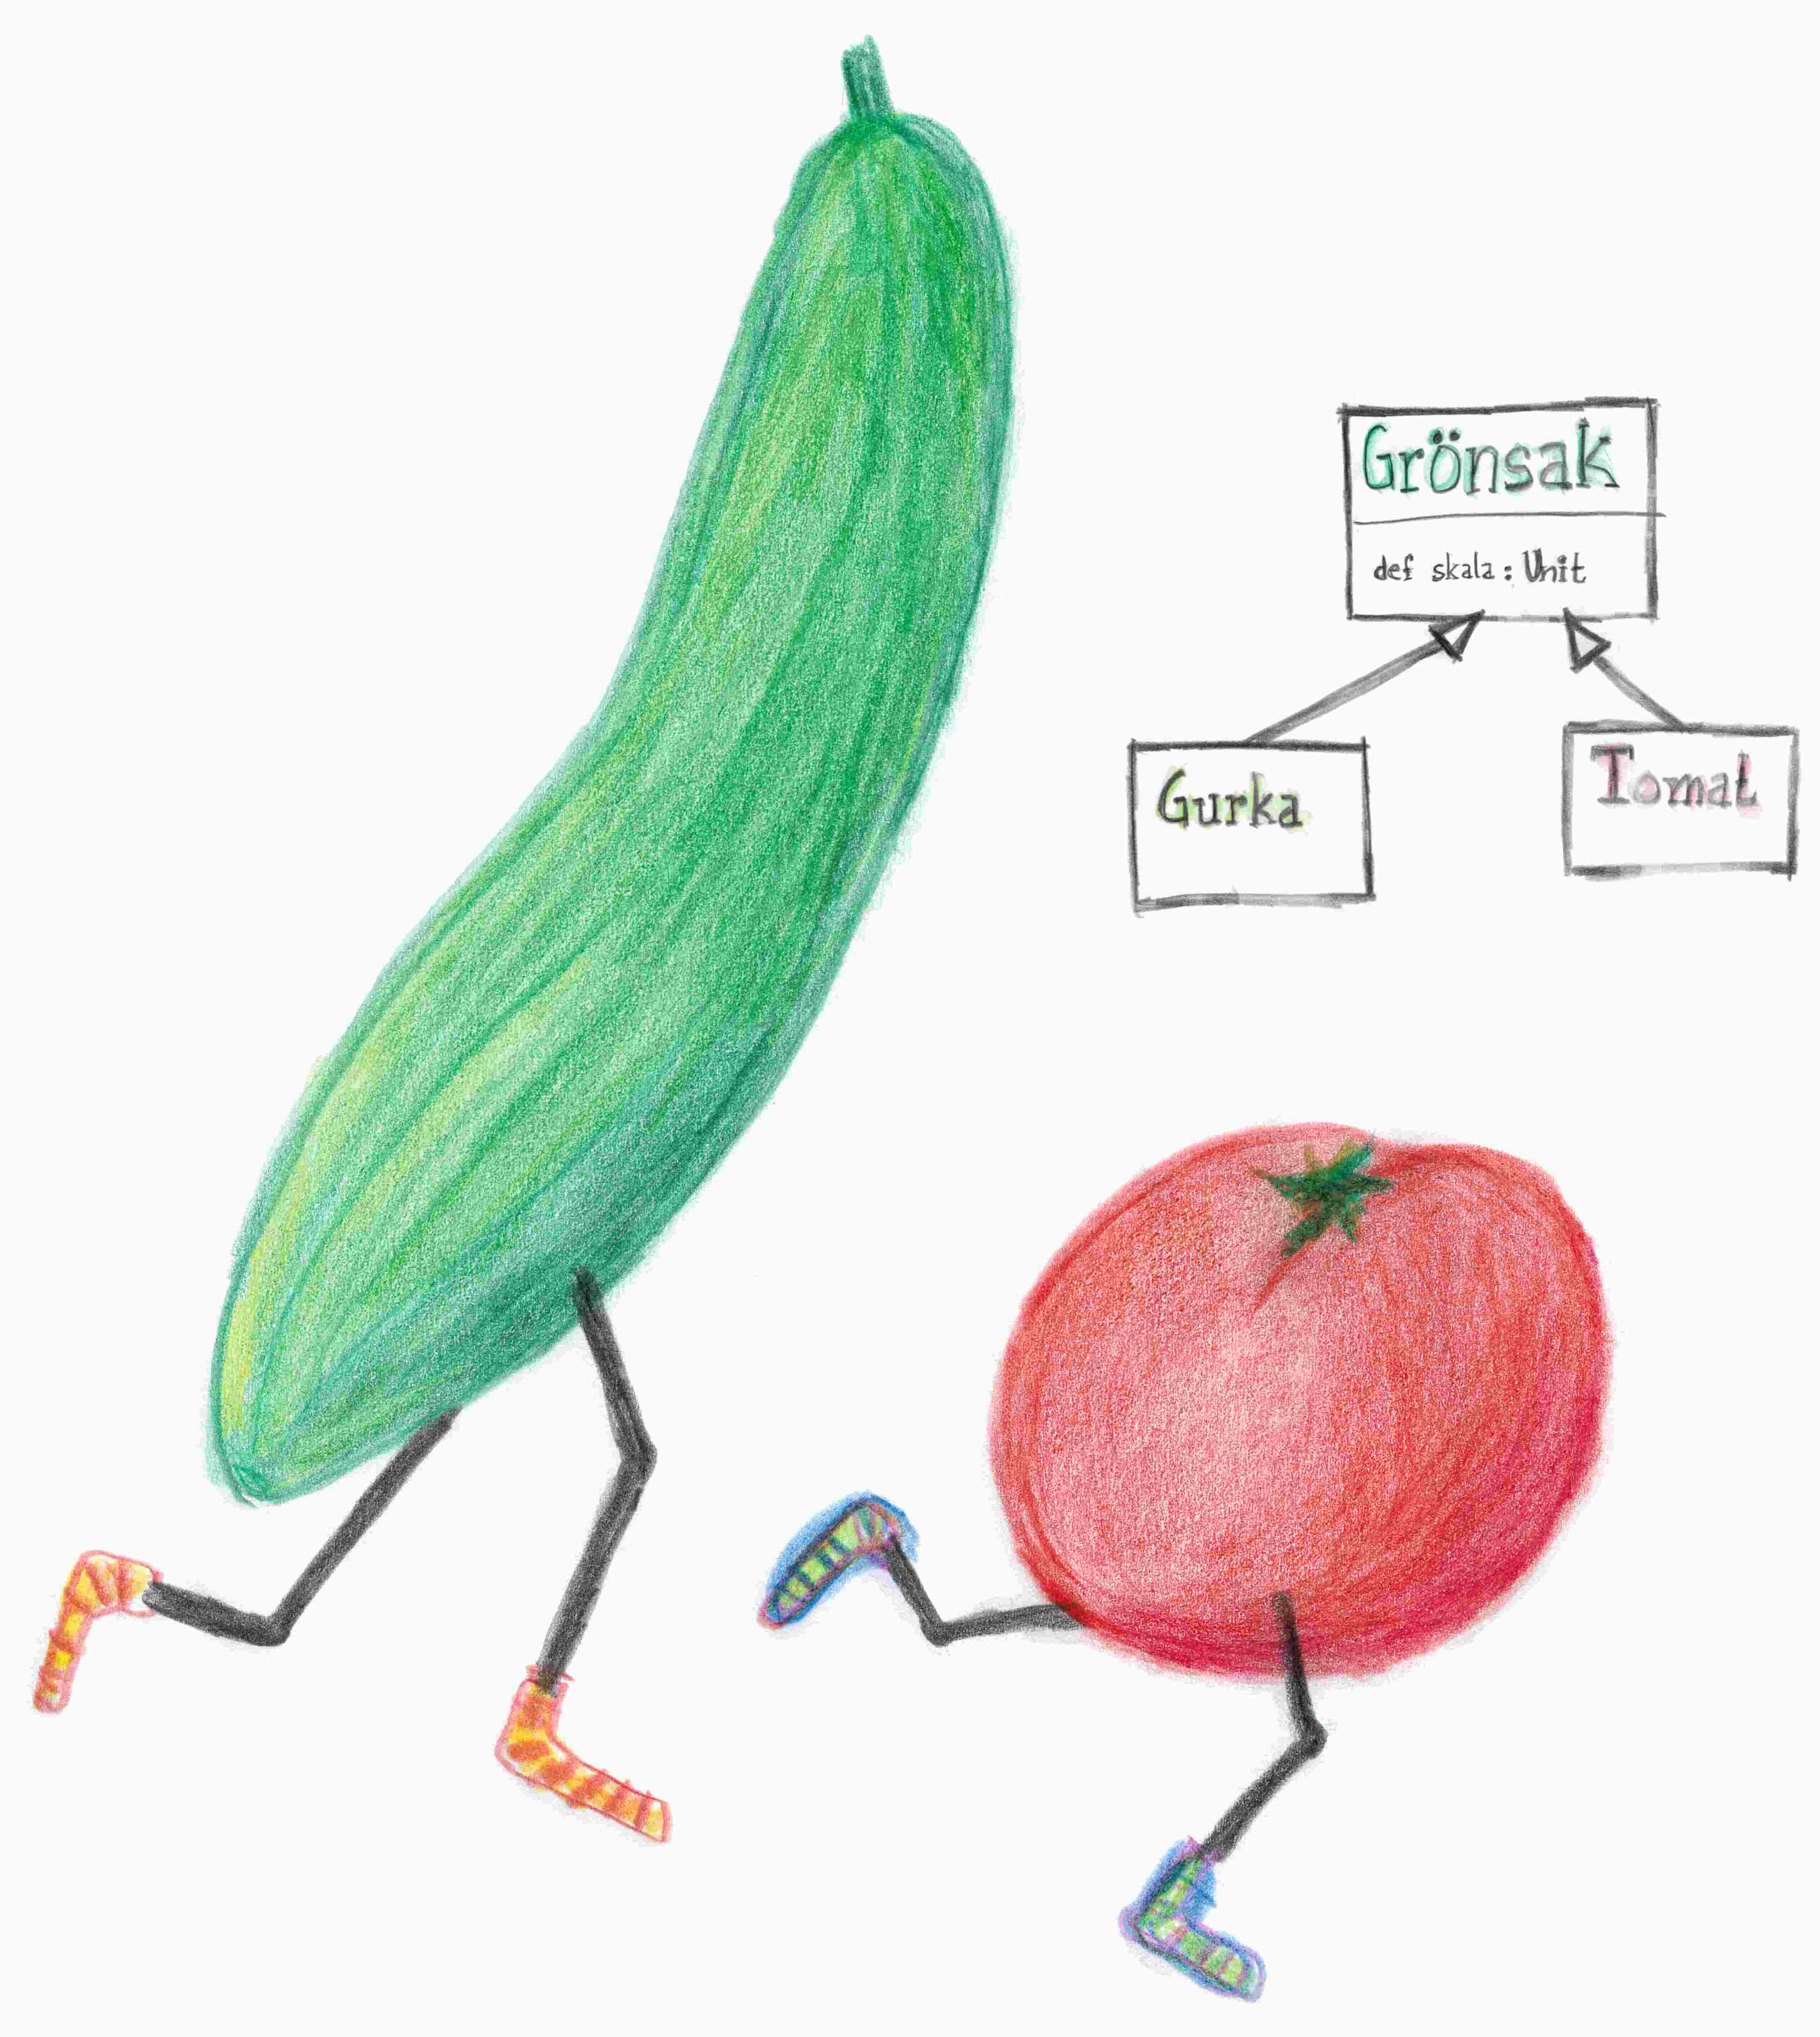
\includegraphics[height=15cm]{cover/gurka.jpg}
}

\author{\fontsize{14}{17}\selectfont Björn Regnell}
\date{\raggedbottom%
\vspace{1em}\begin{minipage}{1.0\textwidth}\centering\fontsize{14}{17}\selectfont
EDAA45, Lp1-2, HT \CurrentYear\\
Datavetenskap, LTH\\
Lunds universitet\\
~\\
Kompileringsdatum: \today \\
\url{http://cs.lth.se/pgk}
\end{minipage}
}

\usepackage{multicol}

\usepackage{pgffor}  %% http://stackoverflow.com/questions/2561791/iteration-in-latex
                     %  allows:  \foreach \n in {1,...,4}{ do something with \n }

\usepackage{framed}  %  allows:   \begin{framed}\end{framed}
%https://ctan.math.illinois.edu/macros/latex/contrib/framed/framed.pdf

% \newenvironment{Slide}[2][]
%  {\begin{oframed}\setlist{noitemsep}\subsection{#2}}
%  {\end{oframed}}

\newenvironment{Slide}[2][]%
  {\setlist{noitemsep}\subsection{#2}}%
  {~\newline\noindent\rule{\textwidth}{0.4pt}}

%\newcommand{\SlideHeading}[1]{\section*{#1}}
\newcommand{\SlideHeading}[1]{\subsection{#1}}

%\usepackage[most]{tcolorbox}
% \newenvironment{Slide}[2][]
%   {\vspace{0.25em}\begin{tcolorbox}[left=1.5em,%width=1.05\textwidth,
%   grow to right by=0.03\textwidth,grow to left by=0.03\textwidth,%breakable,
%   frame hidden,colback=white]\setlist{noitemsep}\SlideHeading{#2}}
%   {\end{tcolorbox}\vspace{0.25em}}



\newcommand{\Subsection}[1]{} %ignore slide sections
\newcommand{\SlideOnly}[1]{} %ignore slide font size

\newif\ifkompendium  % to allow conditional text in slides only showing up in compendium
\kompendiumtrue      % in slides: \kompendiumfalse


\newif\ifPreSolution  % to allow tasks and solutions in same file
\PreSolutiontrue      % in solutions: \PreSolutionfalse

\let\QUESTBEGIN\ifPreSolution  % to mark formatting and numbering of exercises
\let\SOLUTION\else  % to mark solutions in the same file as questions
\let\QUESTEND\fi    % to mark end of exercise


%!TEX encoding = UTF-8 Unicode

\newcommand{\ModWeekONE}{Introduktion}
\newcommand{\ExeWeekONE}{expressions}
\newcommand{\LabWeekONE}{kojo}


\newcommand{\ModWeekTWO}{Program, kontrollstrukturer}
\newcommand{\ExeWeekTWO}{programs}
\newcommand{\LabWeekTWO}{--}


\newcommand{\ModWeekTHREE}{Funktioner, abstraktion}
\newcommand{\ExeWeekTHREE}{functions}
\newcommand{\LabWeekTHREE}{irritext}


\newcommand{\ModWeekFOUR}{Objekt, inkapsling}
\newcommand{\ExeWeekFOUR}{objects}
\newcommand{\LabWeekFOUR}{blockmole}


\newcommand{\ModWeekFIVE}{Klasser, datamodellering}
\newcommand{\ExeWeekFIVE}{classes}
\newcommand{\LabWeekFIVE}{--}


\newcommand{\ModWeekSIX}{Mönster, felhantering}
\newcommand{\ExeWeekSIX}{patterns}
\newcommand{\LabWeekSIX}{blockbattle}


\newcommand{\ModWeekSEVEN}{Sekvenser, enumerationer}
\newcommand{\ExeWeekSEVEN}{sequences}
\newcommand{\LabWeekSEVEN}{shuffle}


\newcommand{\ModWeekEIGHT}{Matriser, typparametrar}
\newcommand{\ExeWeekEIGHT}{matrices}
\newcommand{\LabWeekEIGHT}{life}


\newcommand{\ModWeekNINE}{Mängder, tabeller}
\newcommand{\ExeWeekNINE}{lookup}
\newcommand{\LabWeekNINE}{words}


\newcommand{\ModWeekTEN}{Arv, komposition}
\newcommand{\ExeWeekTEN}{inheritance}
\newcommand{\LabWeekTEN}{snake0}


\newcommand{\ModWeekELEVEN}{Kontextuella abstraktioner, api}
\newcommand{\ExeWeekELEVEN}{context}
\newcommand{\LabWeekELEVEN}{snake1}


\newcommand{\ModWeekTWELVE}{Valfri fördjupning, Projekt}
\newcommand{\ExeWeekTWELVE}{extra}
\newcommand{\LabWeekTWELVE}{Projekt0}


\newcommand{\ModWeekTHIRTEEN}{Repetition}
\newcommand{\ExeWeekTHIRTEEN}{examprep}
\newcommand{\LabWeekTHIRTEEN}{Projekt1}


\newcommand{\ModWeekFOURTEEN}{Muntligt prov}
\newcommand{\ExeWeekFOURTEEN}{Munta}
\newcommand{\LabWeekFOURTEEN}{Munta}


\makeatletter\@twosidefalse\@mparswitchfalse\makeatother
\geometry{inner=45bp,outer=45bp,top=45bp,bottom=45bp} % better for screen reading
\dottedcontents{section}[4.5em]{}{2.9em}{1pc}
\dottedcontents{subsection}[6.5em]{}{4.2em}{1pc}

%\usepackage{tgheros}
%\renewcommand{\familydefault}{\sfdefault}
\begin{document} 

\fontsize{14pt}{17pt}\selectfont  % bigger front better for screen reading
\pagenumbering{roman}

\frontmatter
\maketitle
%!TEX encoding = UTF-8 Unicode
%!TEX root = ../compendium.tex

\clearpage\null\thispagestyle{empty}
\vfill

{
\setlength{\parindent}{0pt}
\emph{Editor}: Björn Regnell \\

%  LIST OF CONTRIBUTORS to https://github.com/lunduniversity/introprog
%    Please contact bjorn.regnell@cs.lth.se if you think you should be
%    on this list, or make a pull request with an update of file briefly
%    describing your contribtion in the commit text.
%    This work is licenced under CC-BY-SA-4.0.
%!TEX encoding = UTF-8 Unicode
%!TEX root = compendium/compendium.tex
\hyphenation{Borg-lund Da-ne-bjer Grampp Palm-qvist Ravn-borg Ro-sen-qvist Schrei-ter Wih-lan-der}
\emph{Contributors} in alphabetical order:
Anders Buhl,
André Philipsson Eriksson,
Anna Axelsson,
Anna Palmqvist Sjövall,
Anton Andersson,
Benjamin Lindberg,
Björn Regnell,
Casper Schreiter,
Cecilia Lindskog,
Dag Hemberg,
Elliot Bräck,
Elsa Cervetti Ogestad,
Emelie Engström,
Emil Wihlander,
Erik Bjäreholt,
Erik Grampp,
Evelyn Beck,
Fredrik Danebjer,
Gustav Cedersjö,
Henrik Olsson,
Hussein Taher,
Jakob Hök,
Jakob Sinclair,
Johan Ravnborg,
Jonas Danebjer,
Jos Rosenqvist,
Maj Stenmark,
Maria Kulesh,
Måns Magnusson,
Nicholas Boyd Isacsson,
Niklas Sandén,
Oliver Persson,
Oscar Sigurdsson,
Oskar Berg,
Oskar Widmark,
Patrik Persson,
Per Holm,
Philip Sadrian,
Sandra Nilsson,
Sebastian Hegardt,
Simon Persson,
Stefan Jonsson,
Theodor Lundqvist,
Tim Borglund,
Tom Postema,
Valthor Halldorsson,
Viktor Claesson,
Wilhelm Wanecek,
William Karlsson.

\\ \newline

\emph{Home}: \url{https://cs.lth.se/pgk} \newline

\emph{Repo}: \url{https://github.com/lunduniversity/introprog} \\ \newline

This compendium is on-going work. \\ \textbf{Contributions are welcome!} \\
\emph{Contact}: \url{bjorn.regnell@cs.lth.se}
\\ \newline

%\emph{Cover art}: Björn Regnell (inspired by Poul Ströyer's illustration of Lennart Hellsing's lyrics to  the childrens song ''Herr Gurka'' with music by Knut Brodin)\\ \newline

~\\ \newline

You can use this work if you respect this \emph{LICENCE}: CC BY-SA 4.0 \\
\url{http://creativecommons.org/licenses/by-sa/4.0/} \\
Please do \emph{not} distribute your solutions to lab assignments and projects.
\\ \newline
Copyright \copyright~ 2015-2017. \\
Dept. of Computer Science, LTH, Lund University. Lund. Sweden.\\
}

%!TEX encoding = UTF-8 Unicode
%!TEX root = ../compendium.tex

\ChapterUnnum{Framstegsprotokoll} 


\subsubsection*{Genomförda övningar}

\vspace{1em}\noindent 
{Till varje laboration hör en övning med uppgifter som utgör förberedelse inför labben. Du behöver minst behärska grundövningarna för att klara labben inom rimlig tid. Om du känner att du behöver öva mer på grunderna, gör då även extrauppgifterna. Om du vill fördjupa dig, gör fördjupningsuppgifterna som är på mer avancerad nivå. Kryssa för nedan vilka övningar du har gjort, så blir lätt för din handledare att se vilka kunskaper du förvärvat hittills.}

\newcommand{\TickBox}{\raisebox{-.50ex}{\Large$\square$}}
\newcommand{\ExeRow}[1]{\texttt{#1} & \TickBox  &  \TickBox &  \TickBox  \\ \addlinespace }

\begin{table}[h]
\centering
\vspace{2em}
\begin{tabular}{lccc}
\toprule \addlinespace 
{\sffamily\small Övning} & 
{\sffamily\small Grund} &	
{\sffamily\small Extra} &
{\sffamily\small Fördjupning}\\ \addlinespace \midrule \\[-0.7em]
\ExeRow{expressions}
\ExeRow{statements}
\ExeRow{functions}
\ExeRow{data}
\ExeRow{vectors}
\ExeRow{classes}
\ExeRow{traits}
\ExeRow{matching}
\ExeRow{matrices}
\ExeRow{sorting}
\ExeRow{scalajava}
\ExeRow{threads}
\bottomrule
\end{tabular}
\end{table}

\newpage

\subsubsection*{Godkända obligatoriska moment}

\vspace{1em}\noindent 
För att bli godkänd på laborationsuppgifterna och projektuppgiften måste du lösa deluppgifterna och diskutera dina lösningar med en handledare. Denna diskussion är din möjlighet att få feedback på dina lösningar. Ta vara på den!
Se till att handledaren noterar nedan när du blivit godkänd på respektive labb. Spara detta blad tills du fått slutbetyg i kursen. 


\vspace{2.5em}\noindent Namn: \dotfill\\

\vspace{1em}\noindent Namnteckning: \dotfill\\

\newcommand{\LabRow}[1]{\\[-1.1em] \texttt{#1} & \dotfill &  \dotfill  \\ \addlinespace }

\begin{table}[h]
\centering
\vspace{1em}
\begin{tabular}{lcc}
\toprule \addlinespace 
{\sffamily\bfseries\small Lab} & {\sffamily\small Datum gk} &	{\sffamily\small Handledares namnteckning}\\ \addlinespace \midrule \\[-0.5em]
%!TEX encoding = UTF-8 Unicode
%!TEX root = ../compendium2.tex
\LabRow{kojo}
\LabRow{irritext}
\LabRow{blockmole}
\LabRow{blockbattle}
\LabRow{shuffle}
\LabRow{words}
\LabRow{life}
\LabRow{snake}
\LabRow{music}
\LabRow{javatext}
\LabRow{survey}
%\toprule 
\addlinespace \midrule \addlinespace
 \\
{\sffamily\small {\bfseries Projektuppgift} (välj en)	} & \dotfill&\dotfill \\ \addlinespace\addlinespace %\midrule
\texttt{( ) bank}  &  &  \\
\texttt{( ) imageprocessing}  \\
\texttt{( ) tictactoe} \\  
\texttt{( ) }\textit{egendefinerad}  \\
\textit{\small Om egen, ge kort beskrivning:}\\
%\dotfill  \\
\bottomrule
\end{tabular}
\end{table}
%!TEX root = ../compendium.tex


\ChapterUnnum{Förord} 

Programmering är inte bara ett sätt att ta makten över systemen som styr vårt samhälle. Det är också ett kraftfullt verktyg för tanken. Att lära sig programmering och systemutveckling är första steget på en livslång resa av kontinuerligt lärande. Programmeringsspråk och utvecklingsverktyg kommer och går, men de grundläggande koncepten sekvens, alternativ, repetition och abstraktion som ligger bakom all mjukvara består. 

Detta kompendium utgör kursmaterial för studier i grundläggande programmering, med syfte att ge en solid bas för ingenjörsstudenter och andra som utvecklar system som innehåller mjukvara. 

Kompendiet är framtaget av, med och för studenter och lärare på universitetsnivå, och distribueras som öppen källkod. Det får användas fritt så länge erkännande ges och eventuella ändringar också publiceras som öppen källkod under samma licens som ursprungsmaterialet. På kursens hemsida \href{http://cs.lth.se/pgk}{cs.lth.se/pgk} och repo \href{http://github.com/lunduniversity/introprog}{github.com/lunduniversity/introprog} finns instruktioner om hur du kan bidra till kursmaterialet.

Läromaterialet fokuserar på lärande genom eget arbete och innehåller övningar och laborationer som är organiserade i moduler. Varje modul har ett tema och tillhörande föreläsningsanteckningar.

I kursen används språken Scala och Java för att illustrera grunderna i imperativ och objektorienterad programmering, tillsammans med elementär funktionsprogrammering. Mer avancerad objektorientering och funktionsprogrammering och  lämnas till fortsättningskurser. 



Den kanske viktigaste framgångsfaktorn vid studier i programmering är att bejaka din egen upptäckarglädje och experimentlusta. Det fantastiska med programmering är att dina egna intellektuella konstruktioner faktiskt \emph{gör} något som just \emph{du} har bestämt! Ta vara på det och prova dig fram genom att koda egna idéer -- det är kul när det funkar men minst lika lärorikt är felsökning, buggrättande och alla misslyckade försök som efter hårt arbete vänds till lyckade lösningar och bestående lärdomar. 

Välkommen i programmeringens fascinerande värld och hjärtligt lycka till med dina studier!




\setcounter{tocdepth}{2} % set headings level in table of contents
\fontsize{13pt}{18pt}\selectfont  % bigger front better for screen reading
\tableofcontents
\mainmatter

\fontsize{13pt}{16pt}\selectfont % bigger front better for screen reading
\pagenumbering{arabic}

\part{Om kursen}
\setcounter{chapter}{-3}
%!TEX root = ../compendium.tex

\ChapterUnnum{Kursens arkitektur}
\begin{framed}
%\noindent\resizebox{\columnwidth}{!}{%
%!TEX encoding = UTF-8 Unicode
\begin{tabular}{l|l|l|l}
\textit{W} & \textit{Modul} & \textit{Övn} & \textit{Lab} \\ \hline \hline
W01 & Introduktion            & expressions & kojo            \\
W02 & Kodstrukturer           & programs    & --              \\
W03 & Funktioner, Objekt      & functions   & bugs            \\
W04 & Datastrukturer          & data        & pirates         \\
W05 & Sekvensalgoritmer       & sequences   & cards           \\
W06 & Klasser, Likhet         & classes     & turtlegraphics  \\
W07 & Arv, Gränssnitt         & traits      & turtlerace-team \\
KS  & KONTROLLSKRIVN.         & --          & --              \\
W08 & Mönster, Undantag       & matching    & chords-team     \\
W09 & Matriser, Typparametrar & matrices    & maze            \\
W10 & Sökning, Sortering      & sorting     & surveydata-team \\
W11 & Scala och Java          & scalajava   & lthopoly-team   \\
W12 & Trådar                  & threads     & life            \\
W13 & Design                  & Uppsamling  & Projekt         \\
W14 & Tentaträning            & Extenta     & --              \\
T   & TENTAMEN                & --          & --              \\
\end{tabular}

%}
\end{framed}

Kursen består av ett antal moduler med tillhörande teori, övningar och laborationer. Genom att göra övningarna bearbetar du teorin och förebereder dig inför laborationerna. När du klarar laborationen i varje modul är du redo att gå vidare till efterkommande modul.  

\newcommand{\Subsection}[1]{} %ignore slide sections

\newenvironment{Slide}[2][]
  {\begin{framed}\setlist{noitemsep}\section*{#2}}
  {\end{framed}}

\newif\ifkompendium
\kompendiumtrue

%!TEX root = ../lect-week01.tex

%%%%%%%%%%%%%%%%%%%%%%%%%%%%%%%%%%%%%%
\Subsection{Om denna kurs}

%%%
\begin{Slide}{Vad och hur?}
\begin{itemize}
\item \emph{Vad} ska du lära dig?
\begin{itemize}
\item Grundläggande principer för programmering\\ $\implies$Inga förkunskaper i programmering krävs!
\item Konstruktion av algoritmer
\item Tänka i abstraktioner
\item Flera olika angreppsätt: imperativ programmering, objektorientering, funktionsprogrammering
\item Programspråken Scala och Java
\item Utvecklingsverktyg (editor, kompilator, utvecklingsmiljö)
\item Implementera, testa, felsöka
\end{itemize}

\item \emph{Hur} ska du lära dig?
\begin{itemize}
\item Genom praktiskt eget arbete: \Emph{Lära genom att göra!}
\item Genom studier av kursens teori: \Emph{Skapa förståelse!}
\item Genom samarbete med dina kurskamrater: \Emph{Gå djupare!}
\end{itemize}
\end{itemize}
\end{Slide}


\ifkompendium
\subsection{hej}
Denna text hamnar bara i kompediet

Hejsan svejsan

\begin{itemize}
\item some item
\end{itemize}


\begin{Code}
hej kod
\end{Code}
\fi


\ifkompendium\else
\begin{Slide}{TESTSLAJD EJ I KOMPENDIUM}
\begin{itemize}
\item \emph{Hej} på dig
\item blablab
\item blabla
\end{itemize}
\begin{Code}
hej kod
\end{Code}
\end{Slide}
\fi


%%%%%%%%%%%%%%%%%%%%%%%%%%%%%%%%%%%%%%
\ifkompendium\else
\Subsection{Meddelande från \href{http://lth.se/code}{Code@LTH}} 
\fi

\begin{itemize}
\item item
\item item
\item item
\item item
\end{itemize}


%!TEX encoding = UTF-8 Unicode
%!TEX root = ../compendium.tex

\ChapterUnnum{Anvisningar}

\SectionUnnum{Samarbetsgrupper}
\subsection*{Samarbetskontrakt}
\subsection*{Grupplaborationer}
\subsection*{Samarbetsbonus}
\SectionUnnum{Föreläsningar}
\SectionUnnum{Övningar}
\SectionUnnum{Laborationer}
 
\begin{itemize}
\item TODO!!! Skriv om pennan och ögat och bocken
\item TODO!!! Skriv att om man inte gör föreberedelserna hinner man inte labben på 2h
\end{itemize}
\SectionUnnum{Resurstider}
\SectionUnnum{Kontrollskrivning}
\SectionUnnum{Tentamen}
%!TEX encoding = UTF-8 Unicode
%!TEX root = ../compendium.tex


\ChapterUnnum{Hur bidra till kursmaterialet?}

%\renewcommand{\SlideHeading}[1]{\subsection{#1}}  %numbering sections in compendium slides

\part{Moduler}
%!TEX encoding = UTF-8 Unicode
%!TEX root = ../compendium1.tex

\renewcommand{\vecka}{1}

\chapter{Introduktion}\label{chapter:W01}
\begin{itemize}[nosep]
\item sekvens
\item alternativ
\item repetition
\item abstraktion
\item programmeringsspråk
\item programmeringsparadigmer
\item editera-kompilera-exekvera
\item datorns delar
\item virtuell maskin
\item värde
\item uttryck
\item variabel
\item typ
\item tilldelning
\item namn
\item val
\item var
\item def
\item if
\item else
\item true
\item false
\item MinValue
\item MaxValue
\item aritmetik
\item slumptal
\item math.random
\item logiska uttryck
\item de Morgans lagar
\item while-sats
\item for-sats
\end{itemize}
\clearpage

%!TEX encoding = UTF-8 Unicode
%!TEX root = ../lect-w01.tex

%%%%%%%%%%%%%%%%%%%%%%%%%%%%%%%%%%%%%%

\Subsection{Att lära denna läsvecka \texttt{w01}}

\ifkompendium\else  %%%%%%%%%%%%%%%%%%%%%%%%%%%%%%%%%%%%%%%%%%%%%%%%%
\begin{SlideExtra}{Att lära denna läsvecka \texttt{w01}}
%!TEX encoding = UTF-8 Unicode

    Modul \Emph{Introduktion}: Övn \Alert{\texttt{expressions}} $\rightarrow$ Labb \Alert{\texttt{kojo}}
    \begin{multicols}{3}\SlideFontTiny
    $\square$ sekvens \\
$\square$ alternativ \\
$\square$ repetition \\
$\square$ abstraktion \\
$\square$ editera \\
$\square$ kompilera \\
$\square$ exekvera \\
$\square$ datorns delar \\
$\square$ virtuell maskin \\
$\square$ litteral \\
$\square$ värde \\
$\square$ uttryck \\
$\square$ identifierare \\
$\square$ variabel \\
$\square$ typ \\
$\square$ tilldelning \\
$\square$ namn \\
$\square$ val \\
$\square$ var \\
$\square$ def \\
$\square$ definera och anropa funktion \\
$\square$ funktionshuvud \\
$\square$ funktionskropp \\
$\square$ procedur \\
$\square$ inbyggda grundtyper \\
$\square$ Int \\
$\square$ Long \\
$\square$ Short \\
$\square$ Double \\
$\square$ Float \\
$\square$ Byte \\
$\square$ Char \\
$\square$ String \\
$\square$ println \\
$\square$ typen Unit \\
$\square$ enhetsvärdet () \\
$\square$ stränginterpolatorn s \\
$\square$ if \\
$\square$ else \\
$\square$ true \\
$\square$ false \\
$\square$ MinValue \\
$\square$ MaxValue \\
$\square$ aritmetik \\
$\square$ slumptal \\
$\square$ math.random \\
$\square$ logiska uttryck \\
$\square$ de Morgans lagar \\
$\square$ while-sats \\
$\square$ for-sats \\
    \end{multicols}
    
\end{SlideExtra}
\fi

\Subsection{Om programmering}

\ifkompendium\else  %%%%%%%%%%%%%%%%%%%%%%%%%%%%%%%%%%%%%%%%%%%%%%%%%

\begin{SlideExtra}{Att skapa koden som styr världen}
\begin{multicols}{2}\footnotesize
I stort sett \Alert{alla} delar av samhället är beroende av programkod:
\begin{itemize}\scriptsize
\item kommunikation
\item transport
\item byggsektorn
\item statsförvaltning
\item finanssektorn
\item media \& underhållning
\item sjukvård
\item övervakning
\item integritet
\item upphovsrätt
\item miljö \& energi
\item sociala relationer
\item utbildning
\item ...
\end{itemize}
\columnbreak %---------
Hur blir ditt framtida yrkesliv som systemutvecklare?
\begin{itemize}
\item  Det är sedan lång tid en \Alert{skriande brist} på utvecklare och det blir bara värre... \\
\href{https://cio.idg.se/2.1782/1.710012/kompetenslarm-jobb-om-fem-ar?queryText=kompetensbrist}{CIO 2018-11-09} %\\
%\href{http://computersweden.idg.se/2.2683/1.663879/oppen-kallkod-brist-kompetens}{CS 2016-08-23} 

\item Störst brist är det på \Emph{kvinnliga} utvecklare: \\
\href{https://www.svt.se/nyheter/inrikes/stor-brist-pa-programmerare-kvinnor-lockas-till-yrket}{SVT 2016-12-03}

\item Global kompetensmarknad \\
  \href{https://cio.idg.se/2.1782/1.648294/hitta-it-kompetens/sida/2/global-rekrytering-aktivt-hr-arbete}{CIO 2016-02-01}\\
  \href{http://computersweden.idg.se/2.2683/1.630901/det-finns-programmerare-och-sa-finns-det-programmerare}{CS 2015-06-14} \\
  \href{http://computersweden.idg.se/2.2683/1.662186/25-miljoner-utvecklare?queryText=miljoner\%20utvecklare}{CS 2016-07-14 }
\end{itemize}
\end{multicols}

\end{SlideExtra}

\begin{SlideExtra}{Utveckling av mjukvara i praktiken}
\begin{itemize}
\item \Emph{Inte bara kodning:} kravbeslut, releaseplanering, design, test, versionshantering, kontinuerlig integration, driftsättning, återkoppling från dagens användare, ekonomi \& investering, gissa om morgondagens användare, ...
\item \Emph{Teamwork:} Inte ensamma hjältar utan autonoma team i decentraliserade organisationer med innovationsuppdrag
\item \Emph{Snabbhet:} Att koda innebär att hela tiden uppfinna nya ''byggstenar'' som ökar organisationens förmåga att snabbt skapa värde med hjälp av mjukvara. \Alert{Öppen källkod}. Skapa kraftfulla API:er.
\item \Emph{Livslångt lärande:} Lär nytt och dela med dig hela tiden. Exempel på pedagogisk utmaning: hjälp andra förstå och använda ditt API $\implies$ \Alert{Samarbetskultur}
\end{itemize}
\end{SlideExtra}


\fi %%%%%%%%%%%%%%%%%%%%%%%%%%%%%%%%%%%%%%%%%%%%%%%%%%%%


% \ifkompendium\else
% \SlideImg{Programming unplugged: Två frivilliga?}{../img/unplugged}
% \SlideImg{Editera och exekvera ett program}{../img/kojo}
% \fi

%%%

\ifkompendium\else
\SlideImg{Vad är en dator?}{../img/eniac}
\fi

\begin{Slide}{Hur fungerar en dator?}
\begin{tikzpicture}[node distance=2.0cm]
\node (input)  [startstop]               {Indata-enhet};
\node (cpu)    [process, below of=input] {CPU};
\node (output) [startstop,below of=cpu]  {Utdata-enhet};

\node (mem) [right of=cpu, xshift=0.4\textwidth, draw = black, thick] {
\begin{minipage}{0.5\textwidth}\centering
\textbf{Minne} med minnesceller
\vspace{1em}

\begin{tabular}{|l | l|}
address & innehåll \\ \hline
0   & 42 \\ \hline
1   & 13 \\ \hline
2   & 18 \\ \hline
3   & 21 \\ \hline
4   & 55 \\ \hline
5   & 64 \\ \hline
6   & 48 \\ \hline
... & ...
\end{tabular}
\end{minipage}
};

\draw [arrow] (input) -- (cpu);
\draw [arrow] (cpu) -- (output);
\draw [arrow] (cpu) -- (mem);
\draw [arrow] (mem) -- (cpu);

\end{tikzpicture}

{\hfill
\begin{minipage}{0.65\textwidth}\vspace{1em}
Minnet innehåller endast \Alert{heltal} som \newline representerar \Emph{data} \Alert{och} \Emph{instruktioner}.
\end{minipage}
}
\end{Slide}

\begin{Slide}{Vad är programmering?}
\begin{itemize}
\item Programmering innebär att ge instruktioner till en maskin.
\item Ett \Emph{programmeringsspråk} används av människor för att skriva \Emph{källkod} som kan översättas av en \Emph{kompilator} till \Emph{maskinspråk} som i sin tur \Emph{exekveras} av en dator.
\end{itemize}


\begin{minipage}{.8\textwidth}
\begin{itemize}
\item Ada Lovelace publicerade det första programmet redan på 1800-talet ämnat för en kugghjulsdator.
\end{itemize}
\end{minipage}%
\begin{minipage}{.2\textwidth}
\centering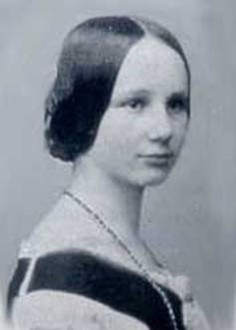
\includegraphics[width=0.6\columnwidth]{../img/ada}
\end{minipage}%
\begin{itemize}
\item \href{https://sv.wikipedia.org/wiki/Programmering}{sv.wikipedia.org/wiki/Programmering}
\item \href{https://en.wikipedia.org/wiki/Computer\_programming}{en.wikipedia.org/wiki/Computer\_programming}
\item Ha picknick i \href{http://kartor.lund.se/wiki/lundanamn/index.php/Ada_Lovelace-parken}{Ada Lovelace-parken} på Brunnshög!
\end{itemize}
\end{Slide}


\begin{Slide}{Vad är en kompilator?}
\begin{minipage}{.35\textwidth}
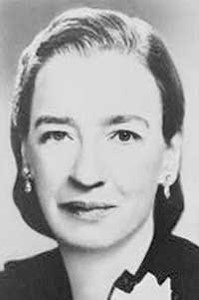
\includegraphics[width=0.6\textwidth]{../img/grace}
\end{minipage}%
\begin{minipage}{.67\textwidth}
%https://www.sharelatex.com/blog/2013/08/29/tikz-series-pt3.html
\begin{tikzpicture}[node distance=1.4cm,scale=0.8]
  \node (input) [startstop] {Källkod};
  \node(inptext) [right of=input, text width=2cm, scale=0.8,xshift=1.5cm]{För\\människor};
  \node (compile) [process, below of=input] {Kompilator};
  \node (output) [startstop, below of=compile] {Maskinkod};
  \node(outtext) [right of=output, text width=2cm, scale=0.8,xshift=1.5cm]{För\\maskiner};
  \draw [arrow] (input) -- (compile);
  \draw [arrow] (compile) -- (output);
  \end{tikzpicture}%

\vspace{1em}\noindent Grace Hopper uppfann kompilatorn 1952. \\ \href{https://en.wikipedia.org/wiki/Grace\_Hopper}{\SlideFontTiny en.wikipedia.org/wiki/Grace\_Hopper}
\end{minipage}%
\end{Slide}


\begin{Slide}{Virtuell maskin (VM) == abstrakt hårdvara}
\begin{multicols}{2}
\begin{itemize}
\item En VM är en ''dator'' implementerad i mjukvara som kan tolka en generell ''maskinkod'' som \Emph{översätts under körning} till den \Alert{verkliga} maskinens specifika maskinkod.

\item Med en VM blir källkoden \Emph{plattformsoberoende} och fungerar på många olika maskiner.

\item Exempel JVM: \\ \Emph{Java Virtual Machine}


\end{itemize}

\columnbreak %---------

%https://www.sharelatex.com/blog/2013/08/29/tikz-series-pt3.html
\begin{tikzpicture}[node distance=1.4cm]
\node (input) [startstop] {Källkod};
\node (compile) [process, below of=input] {Kompilator};
\node (output) [startstop, below of=compile] {Generell ''maskinkod''};
\node (interp) [process, below of=output] {VM interpreterar};
\node (output2) [startstop, below of=interp] {Specifik maskinkod};
\draw [arrow] (input) -- (compile);
\draw [arrow] (compile) -- (output);
\draw [arrow] (output) -- (interp);
\draw [arrow] (interp) -- (output2);
\end{tikzpicture}
\end{multicols}
\end{Slide}

\begin{Slide}{Vad består ett program av?}
\begin{itemize}
\item Text som följer entydiga språkregler (grammatik):
\begin{itemize}
\item \Emph{Syntax}: textens konkreta utseende
\item \Emph{Semantik}: textens betydelse (vad maskinen gör/beräknar)
\end{itemize}
\item \Emph{Nyckelord}: ord med speciell betydelse, t.ex. \code{if}, \code{else}
\item \Emph{Deklarationer}: definitioner av nya ord: \code{def gurka = 42}
\item \Emph{Satser} är instruktioner som \Alert{gör} något: \code{print("hej")}
\item \Emph{Uttryck} är instruktioner som beräknar ett \Alert{resultat}: \code{1 + 1}
\item \Emph{Data} är information som behandlas: t.ex. heltalet \code{42}
\item Instruktioner ordnas i kodstrukturer: \Alert{SARA}
\begin{itemize}
  \item \Emph{Sekvens}: ordningen spelar roll för vad som händer
  \item \Emph{Alternativ}: olika resultat beroende på uttrycks värde
  \item \Emph{Repetition}: instruktioner upprepas många gånger
  \item \Emph{Abstraktion}: nya byggblock skapas för att återanvändas
\end{itemize}
\end{itemize}
\end{Slide}

\begin{Slide}{Exempel på programmeringsspråk}
Det finns massor med olika språk och det kommer ständigt nya.
\vspace{1em}
\begin{multicols}{2}
Exempel:
\begin{itemize}
\item Java
\item C
\item C++
\item C\#
\item Python
\item JavaScript
\item Scala
\end{itemize}

\columnbreak %---------

Topplistor:
\begin{itemize}
\item \href{https://redmonk.com/sogrady/2020/07/27/language-rankings-6-20/}{Redmonk language rankings}   
%\item \href{https://redmonk.com/sogrady/2019/07/18/language-rankings-6-19/}{Redmonk language rankings}   
%\item \href{https://redmonk.com/sogrady/2018/08/10/language-rankings-6-18/}{Redmonk language rankings}   
\item \href{http://pypl.github.io/PYPL.html}{PYPL Index}
\item \href{http://www.tiobe.com/index.php/content/paperinfo/tpci/index.html}{TIOBE Index}
\end{itemize}
% \vspace{1em}
% 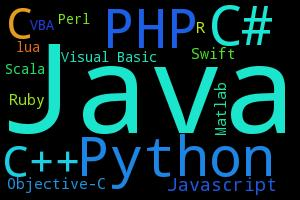
\includegraphics[width=0.8\columnwidth]{../img/pypl}\\\SlideFontSmall{[PYPL (2016)]}
\end{multicols}

\end{Slide}

\ifkompendium\else
\begin{SlideExtra}{Redmonk Language Rankings: Github, Stackoverflow}
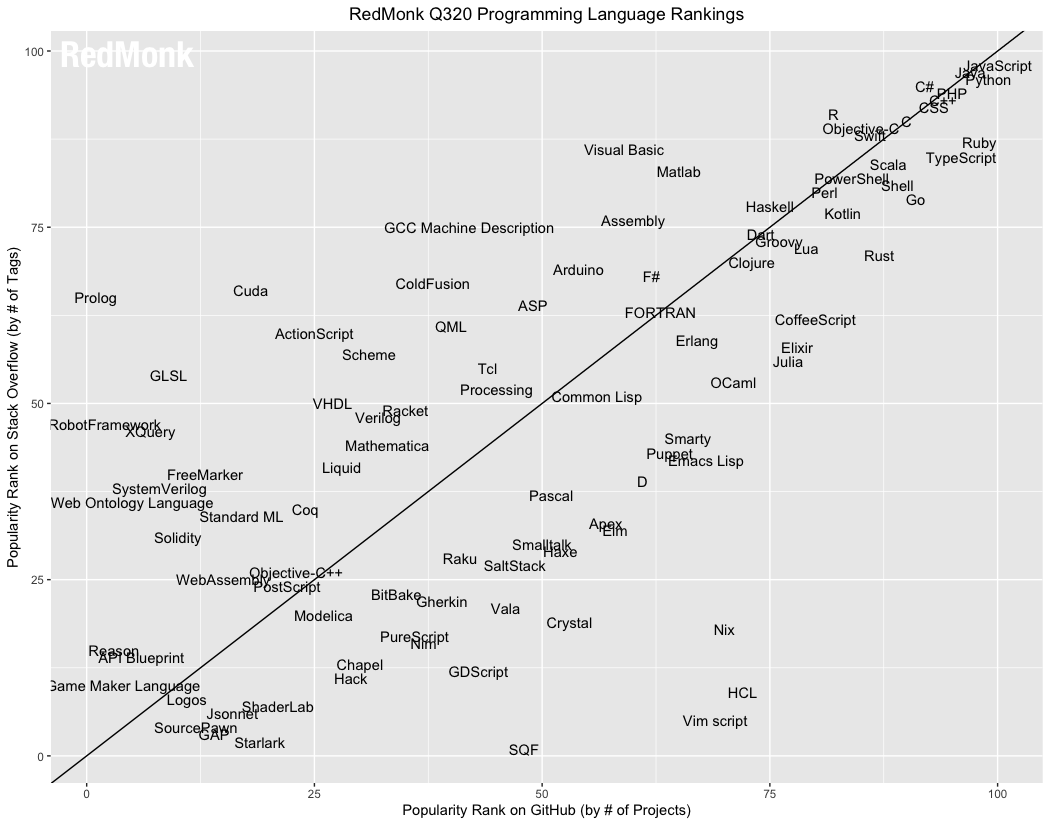
\includegraphics[width=0.95\columnwidth]{../img/redmonk-Q320}
\end{SlideExtra}
\begin{SlideExtra}{Några språks utveckling över tid enl. PYPL}
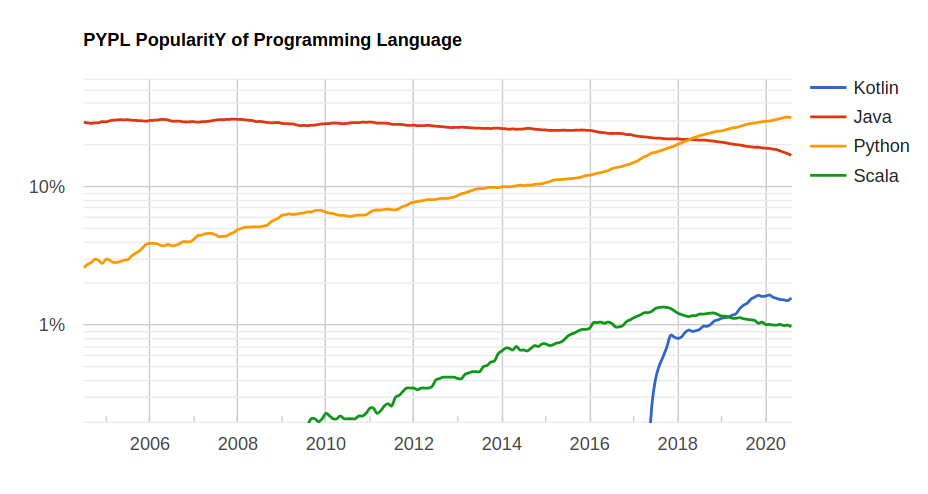
\includegraphics[width=0.95\columnwidth]{../img/pypl-06-20}
\end{SlideExtra}

\fi

\begin{Slide}{Olika programmeringsparadigm}
\begin{itemize}
\item Det finns många olika \href{https://en.wikipedia.org/wiki/Programming_paradigm}{programmeringsparadigm} (sätt att programmera på), till exempel:
\begin{itemize}\SlideFontSmall
\item \Emph{imperativ programmering:} programmet är uppbyggt av sekvenser av olika satser som påverkar systemets tillstånd
\item \Emph{objektorienterad programmering:} en sorts imperativ programmering där programmet består av objekt som sammanför data och operationer på dessa data
\item \Emph{funktionsprogrammering:} programmet är uppbyggt av samverkande (matematiska) funktioner som undviker föränderlig data och tillståndsändringar
\item \Emph{deklarativ programmering, logikprogrammering:} programmet är uppbyggt av logiska uttryck som beskriver olika fakta eller villkor och exekveringen utgörs av en bevisprocedur som söker efter värden som uppfyller fakta och villkor
\end{itemize}
\end{itemize}
\end{Slide}


\begin{Slide}{Hello world}

Scala-skript:
\begin{REPLnonum}
scala> println("Hello World!")
Hello World!
\end{REPLnonum}

Scala-applikation:
\begin{Code}
object Hello {
  def main(args: Array[String]): Unit = println("Hello world!")
}
\end{Code}

Java-applikation:
\begin{Code}[language=Java]
public class Hello {
    public static void main(String[] args) {
        System.out.println("Hello world!");
    }
}
\end{Code}

\end{Slide}

\begin{Slide}{Utvecklingscykeln}
editera; kompilera; hitta fel och förbättringar; editera; kompilera; hitta fel och förbättringar; editera; kompilera; hitta fel och förbättringar; editera; kompilera; hitta fel och förbättringar; editera; kompilera; hitta fel och förbättringar; editera; kompilera; hitta fel och förbättringar; ...

\begin{Code}
upprepa(1000){
  editera
  kompilera
  testa
}
\end{Code}
\end{Slide}

\begin{Slide}{Utvecklingsverktyg}
\begin{itemize}
\item Din verktygskunskap är mycket viktig för din produktivitet.
\item Lär dig kortkommandon för vanliga handgrep.
\item Verktyg vi använder i kursen:
\begin{itemize}
\item Scala \Emph{REPL}: från övn 1
\item \Emph{Texteditor} för kod, t.ex VS \code{code}: från övn 2
\item Kompilera med \Emph{\code{scalac}} och \Emph{\code{javac}}: från övn 2
\item Integrerad utvecklingsmiljö (IDE)
\begin{itemize}
\item \Emph{Kojo}: från lab 1
\item \Emph{IntelliJ IDEA} (alt. ScalaIDE/Eclipse): från läsperiod 2
\end{itemize}
\item \Emph{jar} för att packa ihop och distribuera klassfiler
\item \Emph{javadoc} och \Emph{scaladoc} för dokumentation av kodbibliotek
\end{itemize}
\item Andra verktyg som är bra att lära sig:
\begin{itemize}
\item git för versionshantering
\item GitHub för kodlagring -- men \Alert{inte} av lösningar till labbar!
\end{itemize}
\end{itemize}
\end{Slide}





\Subsection{De enklaste beståndsdelarna: litteraler, uttryck, variabler}


\begin{Slide}{Litteraler}
\begin{itemize}
\item En literal representerar ett fixt \Emph{värde} i koden och används för att skapa \Alert{data} som programmet ska bearbeta.
\item Exempel: \\
\begin{tabular}{l l}
\code|42| & heltalslitteral\\
\code|42.0| & decimaltalslitteral\\
\code|'!'| & teckenlitteral, omgärdas med 'enkelfnuttar' \\
\code|"hej"| & stränglitteral, omgärdas med ''dubbelfnuttar'' \\
\code|true| & litteral för sanningsvärdet ''sant''\\
\end{tabular}
\item Literaler har en \Emph{typ} som avgör vad man kan göra med dem.
\end{itemize}
\end{Slide}

\begin{Slide}{Exempel på inbyggda datatyper i Scala}\SlideFontSmall
\begin{itemize}
\item Alla värden, uttryck och variabler har en \href{https://sv.wikipedia.org/wiki/Datatyp}{\Emph{datatyp}}, t.ex.:
\begin{itemize}\footnotesize
\item \code{Int} för heltal
\item \code{Long} för \textit{extra} stora heltal (tar mer minne)
\item \code{Double} för decimaltal, så kallade flyttal med flytande decimalpunkt
\item \code{String} för strängar
\end{itemize}

\item Kompilatorn håller reda på att uttryck kombineras på ett \Emph{typsäkert} sätt. Annars blir det \Alert{kompileringsfel}.

\item Scala och Java är s.k. \href{https://sv.wikipedia.org/wiki/Typsystem}{\Emph{statiskt typade}} språk, vilket innebär att kontroll av typinformation sker vid kompilering \Eng{compile time}\footnote{Andra språk, t.ex. Python och Javascript är \Emph{dynamiskt typade} och där skjuts typkontrollen upp till körningsdags \Eng{run time} \\ Vilka är för- och nackdelarna med statisk vs. dynamisk typning?}.

\item Scala-kompilatorn gör \href{https://en.wikipedia.org/wiki/Type_inference}{\Emph{typhärledning}}: man \Alert{slipper skriva typerna} om kompilatorn kan lista ut dem med hjälp av typerna hos deluttrycken.

\end{itemize}
\end{Slide}


\begin{Slide}{Grundtyper i Scala}\SlideFontSmall
Dessa \Emph{grundtyper} \Eng{basic types} finns inbyggda i Scala:

\begin{table}[H]
\renewcommand{\arraystretch}{1.4}
\begin{tabular}{p{0.24\textwidth}|p{0.21\textwidth}|l}
\textit{Svenskt namn} & \textit{Engelskt namn} & \Emph{Grundtyper} \\ \hline
heltalstyp & integral type & \texttt{Byte}, \texttt{Short}, \texttt{Int}, \texttt{Long}, \texttt{Char} \\
flyttalstyp  &  floating point \newline number types & \texttt{Float}, \texttt{Double} \\
numeriska typer & numeric types & heltalstyper och flyttalstyper \\
strängtyp \newline (teckensekvens) & string type & \texttt{String}  \\
sanningsvärdestyp  \newline (boolesk typ)& truth value type & \texttt{Boolean} \\
\end{tabular}
\end{table}

\end{Slide}

\begin{Slide}{Grundtypernas implementation i JVM}\SlideFontSmall
\begin{table}[H]
\renewcommand{\arraystretch}{1.4}
\begin{tabular}{l|l|l|l}
\Alert{Grundtyp} i &  Antal                &      Omfång&\Alert{primitiv typ} i\\
 \Emph{Scala} & bitar & minsta/största värde &\Emph{Java} \& \Emph{JVM}\\ \hline
\texttt{Byte}   &  8  & $-2^7$ ... $2^7-1$   & \texttt{byte} \\
\texttt{Short}  &  16 & $-2^{15}$ ... $2^{15}-1$ & \texttt{short} \\
\texttt{Char}   &  16 & $0$ ... $2^{16}-1$ & \texttt{char} \\
\texttt{Int}    &  32 & $-2^{31}$ ... $2^{31}-1$ & \texttt{int} \\
\texttt{Long}   &  64 & $-2^{63}$ ... $2^{63}-1$ & \texttt{long} \\
\texttt{Float}  &  32 & ± $3.4028235 \cdot 10^{38}$  & \texttt{float} \\
\texttt{Double} &  64 & ± $1.7976931348623157 \cdot 10^{308}$ & \texttt{double} \\
\end{tabular}
\end{table}

Grundtypen \texttt{String} lagras som en \emph{sekvens} av 16-bitars tecken av typen \texttt{Char} och kan vara av godtycklig längd (tills minnet tar slut).

\end{Slide}


\begin{Slide}{Uttryck}
\begin{itemize}
\item Ett \Emph{uttryck} består av en eller flera delar som efter \Emph{evaluering} ger ett \Alert{resultat}.
\item Delar i ett uttryck kan t.ex. vara: \\ literaler (42), operatorer (+), funktioner (sin), ...
\item Exempel:
\begin{itemize}
\item Ett enkelt uttryck: \\ \code{42.0}
\item Sammansatta uttryck: \\
\code{40 + 2} \\
\code{(20 + 1) * 2} \\
\code{sin(0.5 * Pi)} \\
\code{"hej" + " på " + "dej"}
\end{itemize}

\item När programmet tolkas sker \Emph{evaluering} av uttrycket, vilket ger ett resultat i form av ett \Emph{värde} som har en \Emph{typ}.
\end{itemize}
\end{Slide}


\begin{Slide}{Variabler}\SlideFontSmall
\begin{itemize}
\item En \Emph{variabel} kan tilldelas värdet av ett enkelt eller sammansatt uttryck.
\item En variabel har ett \Emph{variabelnamn}, vars utformning följer språkets regler för s.k. \Emph{identifierare}.
\item En ny variabel införs i en \Emph{variabeldeklaration} och då den kan ges ett värde, \Emph{initialiseras}. Namnet användas som \Emph{referens} till värdet.
\item Exempel på variabeldeklarationer i Scala, notera \Emph{nyckelordet} \code{val}:
\begin{Code}
val a = 0.5 * Pi
val length = 42 * sin(a)
val exclamationMarks = "!!!"
val greetingSwedish = "Hej på dej" + exclamationMarks
\end{Code}

\item Vid exekveringen av programmet lagras variablernas värden i minnet och deras respektive värde hämtas ur minnet när de \Emph{refereras}.

\item Variabler som deklareras med \code{val} kan endast tilldelas ett värde \Alert{en enda gång}, vid den initialisering som sker vid deklarationen.
\end{itemize}

\end{Slide}


\begin{Slide}{Regler för identifierare}
\begin{itemize}
\item \Emph{Enkel} identifierare: t.ex. \code{gurka2tomat}
\begin{itemize}
\item Börja med bokstav
\item ...följt av bokstäver eller siffror
\item Kan även innehålla understreck
\end{itemize}

\item \Emph{Operator}-identifierare, t.ex. \code{+:}
\begin{itemize}
\item Börjar med ett \Emph{operatortecken}, t.ex. \code{+ - * / : ? ~ #}
\item Kan följas av fler operatortecken
\end{itemize}


\item En identifierare får \Alert{inte} vara ett \Emph{reserverat ord}, se \href{http://cs.lth.se/pgk/quickref}{snabbreferensen} för alla reserverade ord i Scala \& Java.

\item \Emph{Bokstavlig} identifierare: \code{`kan innehålla allt`}
\begin{itemize}
\item Börjar och slutar med \Emph{backticks}  \code{` `}
\item Kan innehålla vad som helst (utom backticks)
\item Kan användas för att undvika krockar med reserverade ord: \texttt{\code{`}val\code{`}}
\end{itemize}

\end{itemize}
\end{Slide}



%\begin{Slide}{Regler för identifierare i Java}\footnotesize
%När kompilatorn ''läser''  \footnote{man säger ofta ''parsa'' i stället för ''läsa'' när kompilatorn tolkar koden} koden och och försöker hitta variabelnamn, antar den att du följer de entydiga syntaktiska reglerna för språket.  \\ \vskip1em För namn i Java gäller följande regler: %https://docs.oracle.com/javase/tutorial/java/nutsandbolts/variables.html
%\begin{itemize}
%\item Namn får inte vara \href{https://docs.oracle.com/javase/tutorial/java/nutsandbolts/_keywords.html}{reserverade ord}
%\item Stora och små bokstäver spelar roll \Eng{case sensistive} \\ \lstinline{int highScore;} och \lstinline{int highscore;} ger alltså två \textit{olika} variabler
%\item Namnet måste börja med en bokstav, ett understreck \_ eller ett dollartecken \$
%\item Namn får \textit{inte} innehålla blanktecken
%\item Namn får innehålla bokstäver, siffror, understreck \_ och dollartecken \$, men \textit{inte} andra specialtecken (alltså inte \lstinline~%&@!{(})/+-*~ etc.)
%\end{itemize}
%\end{Slide}



\begin{Slide}{Att bygga strängar: konkatenering och interpolering}
\begin{itemize}
\item Man kan \Emph{konkatenera} strängar med operatorn + \\ \code{"hej" + " på " + "dej"}
\item Efter en sträng kan man konkatenera vilka uttryck som helst; uttryck inom parentes evalueras först och värdet görs sen om till en sträng före konkateneringen:
\begin{Code}
val x = 42
val msg = "Dubbla värdet av " + x + " är " + (x * 2) + "."
\end{Code}
\item Man kan i Scala (men inte Java) få hjälp av kompilatorn att övervaka bygget av strängar med \Emph{stränginterpolatorn} \Alert{s}:
\begin{Code}
val msg = s"Dubbla värdet av $x är ${x * 2}."
\end{Code}

\end{itemize}
\end{Slide}

\begin{Slide}{Heltalsaritmetik}\SlideFontSmall
\begin{itemize}
\item De fyra räknesätten skrivs som i matematiken (vanlig \href{https://en.wikipedia.org/wiki/Order_of_operations}{precedens}):
\begin{REPL}
scala> 3 + 5 * 2 - 1
res0: Int = 12
\end{REPL}
\item \Emph{Parenteser} styr \Alert{evalueringsordningen}:
\begin{REPL}
scala> (3 + 5) * (2 - 1)
res1: Int = 8
\end{REPL}
\item \Emph{Heltalsdivision} sker med \Alert{decimaler avkortade}:
\begin{REPL}
scala> 41 / 2
res2: Int = 20
\end{REPL}
\item \href{https://en.wikipedia.org/wiki/Modulo_operation}{\Emph{Moduloräkning}} med restoperatorn \code{%}
\begin{REPL}
scala> 41 % 2
res3: Int = 1
\end{REPL}
\end{itemize}
\end{Slide}


\begin{Slide}{Flyttalsaritmetik}\SlideFontSmall
\begin{itemize}
\item Decimaltal representeras med s.k. \href{https://sv.wikipedia.org/wiki/Flyttal}{\Emph{flyttal}} av typen \code{Double}:
\begin{REPL}
scala> math.Pi
res4: Double = 3.141592653589793
\end{REPL}

\item Stora tal så som $\pi*10^{12}$ skrivs:
\begin{REPL}
scala> math.Pi * 1E12
res5: Double = 3.141592653589793E12
\end{REPL}
\item Det finns \Alert{inte} oändligt antal decimaler vilket ger problem med \Alert{avvrundingsfel}:
\begin{REPL}
scala> 0.0000000000001
res6: Double = 1.0E-13

scala> 1E10 + 0.0000000000001
res7: Double = 1.0E10
\end{REPL}
\end{itemize}
\end{Slide}

% \ifkompendium\else
% \begin{SlideExtra}{På rasten}
% En per grupp kommer fram hit och tar en grupp-skylt
% \begin{itemize}
%   \item Samlas i era samarbetsgrupper i foajen
%   \item D1.01a längst västerut (mot havet), D1.12b längst österut
%   \item Lär allas namn
%   \item Bestäm tid för första möte
%   \item Vid behov: \\ Bestäm vem som mejlar till de i gruppen som inte är här idag 
% \end{itemize}  
% \end{SlideExtra}
% \fi

\Subsection{Funktioner}

\begin{Slide}{Definiera namn på uttryck}
\begin{itemize}
\item Med nyckelordet \code{def} kan man låta ett \Emph{namn} betyda samma sak som ett \Emph{uttryck}.
\item Exempel:
\begin{Code}
def gurklängd = 42 + x
\end{Code}
\item Uttrycket till höger evalueras \Alert{varje} gång \Emph{anrop} sker,\\
d.v.s. varje gång namnet används på annat ställe i koden.
\begin{Code}
gurklängd
\end{Code}

\end{itemize}
\end{Slide}

\begin{Slide}{Funktion, argument, parameter}\SlideFontSmall
\begin{itemize}
\item En \Emph{funktion} räknar ut \Alert{resultat} baserat på indata som kallas \Emph{argument}.

\item Argument ges namn genom deklaration av \Emph{parametrar}.

\item Exempel på deklaration av en funktion med en parameter:
\begin{Code}
def dubblera(x: Int) = 2 * x
\end{Code}

\item Parametrarnas typ \Alert{måste} beskrivas efter \Emph{kolon}.
\item Kompilatorn kan härleda \Emph{returtypen}, men den kan också med fördel, för tydlighetens skull, anges \Alert{explicit}:
\begin{Code}
def dubblera(x: Int): Int = 2 * x
\end{Code}

\item Observera att namnet \code{x} blir ett ''nytt fräscht'' \Emph{lokalt namn} som \Alert{bara finns och syns  ''inuti'' funktionen} och har inget med ev. andra \code{x} utanför funktionen att göra.

\item Beräkningen sker först vid \Alert{anrop} av funktionen:
\begin{REPL}
scala> dubblera(42)
res1: Int = 84
\end{REPL}

\end{itemize}
\end{Slide}






\begin{Slide}{Färdiga matte-funktioner i paketet \texttt{scala.math}}\SlideFontSmall
\begin{itemize}
\item I paketet \texttt{\Emph{scala.math}} finns många användbara funktioner: t.ex.\\
\code{math.random()} ger slumptal mellan \code{0.0} och \code{0.99999999999999999}
\begin{REPLnonum}
scala> val x = math.random()
x: Double = 0.27749191749889635

scala> val length = 42.0 * math.sin(math.Pi / 3.0)
length: Double = 36.373066958946424
\end{REPLnonum}

\item Studera dokumentationen här: \\{\SlideFontTiny
\url{http://www.scala-lang.org/api/current/scala/math/}}

\item Paketet \code{scala.math} delegerar ofta till Java-klassen \texttt{\Emph{java.lang.Math}} som är dokumenterad här: \\{\SlideFontTiny
\url{https://docs.oracle.com/javase/8/docs/api/java/lang/Math.html}}

\end{itemize}
\end{Slide}



\Subsection{Logik}

\begin{Slide}{Logiska uttryck}\SlideFontSmall
\begin{minipage}{.8\textwidth}
\begin{itemize}
\item Datorn kan ''räkna'' med sanning och falskhet: \\
s.k. \href{https://en.wikipedia.org/wiki/Boolean_algebra}{booelsk algebra} efter \href{https://en.wikipedia.org/wiki/George_Boole}{George Boole}

\item Enkla logiska uttryck: (finns bara två stycken)
\begin{itemize}
\item[] \code{true}
\item[] \code{false}
\end{itemize}
\end{itemize}
\end{minipage}%
\begin{minipage}{.2\textwidth}
\centering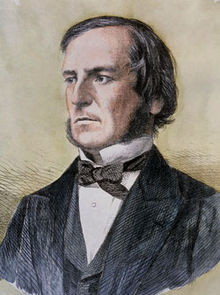
\includegraphics[width=0.9\columnwidth]{../img/boole}
\end{minipage}%
\begin{itemize}


\item Sammansatta logiska uttryck med logiska operatorer:\\
\code{&&} och, \texttt{||} eller, \texttt{!} icke, \code{==} likhet, \code{!=} olikhet,
relationer: \code{> < >= <=}

\item Exempel:
\begin{itemize}
\item[] \code{true && true}
\item[] \code{false || true}
\item[] \code{!false}
\item[] \code{42 == 43}
\item[] \code{42 != 43}
\item[] \code{(42 >= 43) || (1 + 1 == 2)}
\end{itemize}

\end{itemize}
\end{Slide}

\begin{Slide}{De Morgans lagar}

\href{https://en.wikipedia.org/wiki/Augustus_De_Morgan}{\Emph{De Morgans lagar}} beskriver vad som händer om man \Alert{negerar} ett logiskt uttryck. Kan användas för att göra \Emph{förenklingar}.

%$p$ och $q$ är logiska uttryck, $\neg$ står för ''icke'', $\wedge$ för ''och'', $\vee$ för ''eller'':
%\begin{eqnarray*}
%\neg (p \wedge q) & \Longleftrightarrow & (\neg p) \vee (\neg q)\\
%\neg (p \vee q) & \Longleftrightarrow & (\neg p) \wedge (\neg q)\\
%\end{eqnarray*}

\begin{itemize}
\item I all deluttryck sammanbundna med \code{&&} eller \code{||}, \\ ändra alla \code{&&} till \code{||} och omvänt.
\item Negera alla ingående deluttryck. En relation negeras genom att man byter \texttt{==} mot \texttt{!=}, \texttt{<} mot \texttt{>=}, etc.
\end{itemize}

Exempel på förenkling där de Morgans lagar används upprepat:

\begin{Code}[escapechar=X,backgroundcolor=,frame=none,basicstyle=\ttfamily\fontsize{10}{12}\selectfont]
! (a < b || (a == 1 && b == 1))             X$\iff$X
! (a < b) && ! (a == 1 && b == 1)           X$\iff$X
! (a < b) && (! (a == 1) || ! (b == 1))     X$\iff$X
a >= b && (a != 1 || b != 1)
\end{Code}
\end{Slide}

\begin{Slide}{Alternativ med if-uttryck}
\begin{itemize}
\item Ett if-uttryck börjar med nyckelordet \code{if}, följt av ett logiskt uttryck inom parentes och två grenar.
\begin{Code}
def slumpgrönsak = if (math.random() < 0.8) "gurka" else "tomat"
\end{Code}
\item Den ena grenen evalueras om uttrycket är \code{true}
\item Den andra \code{else}-grenen evalueras om uttrycket är \code{false}
\begin{REPLnonum}
scala> slumpgrönsak
res13: String = gurka

scala> slumpgrönsak
res14: String = gurka

scala> slumpgrönsak
res15: String = tomat

\end{REPLnonum}
\end{itemize}
\end{Slide}

\Subsection{Satser}


%%%%%%%%%%%%%%%%%%%%%%%%
\begin{Slide}{Variabeldeklaration och tilldelningssats}\SlideFontTiny

\begin{itemize}
\item En \Emph{variabeldeklaration} medför att \Alert{plats i datorns minne} reserveras så att värden av den typ som variabeln kan referera till får plats där.

\item Vid deklaration ska variabeln \Emph{initialiseras} med ett startvärde.

\item En \code{val}-deklaration ger en variabel som efter initialisering inte kan ändras.


\begin{multicols}{2}
Dessa deklarationer...
\begin{lstlisting}
var x = 42
val y = x + 1
\end{lstlisting}
... ger detta innehåll någonstans i minnet:

%http://tex.stackexchange.com/questions/18521/tikz-matrix-as-a-replacement-for-tabular
\begin{tikzpicture}[]
\matrix [matrix of nodes, row sep=0, column 2/.style={nodes={rectangle,draw,minimum width=3em}}]
{
x   & 42 \\
y   & 43 \\
};
\end{tikzpicture}
%\end{column}

%\end{columns}

\end{multicols}


\item Med en \Emph{tilldelningssats} ges en tidigare \code{var}-deklarerad variabel ett nytt värde:
\begin{lstlisting}
x = 13
\end{lstlisting}

\item Det gamla värdet försvinner för alltid och det nya värdet lagras istället: \\
\begin{tikzpicture}[]
\matrix [matrix of nodes, row sep=0, column 2/.style={nodes={rectangle,draw,minimum width=3em}}]
{
x   & 13 \\
y   & 43 \\
};
\end{tikzpicture}

Observera att \code{y} här inte påverkas av att x ändrade värde.
\end{itemize}
\end{Slide}

\begin{Slide}{Tilldelningssatser är \emph{inte} matematisk likhet}\SlideFontSmall

\begin{itemize}

\item Likhetstecknet används alltså för att \Emph{tilldela} variabler nya värden och det är \Alert{inte} samma sak som matematisk likhet. Vad händer här?
\begin{lstlisting}
x = x + 1
\end{lstlisting}

\item Denna syntax är ett arv från de gamla språken C, Fortran mfl.

\item I \href{https://en.wikipedia.org/wiki/Assignment_(computer_science)}{andra språk} används  t.ex.  \\\vspace{1em}
\texttt{x := x + 1}  \hspace{2em} eller  \hspace{2em} \texttt{x <- x + 1} \\\vspace{0.5em}

\item Denna syntax visar kanske bättre att tilldelning är en \Emph{stegvis process}:

\begin{enumerate}\SlideFontTiny
\item Först beräknas \Emph{uttrycket till höger} om tilldelningstecknet.
\item Sedan \Emph{ersätts värdet} som variabelnamnet refererar till av det beräknade uttrycket. Det gamla värdet \Alert{försvinner för alltid}.
\end{enumerate}

\end{itemize}

\end{Slide}


\begin{Slide}{Förkortade tilldelningssatser}
\begin{itemize}
\item Det är vanligt att man vill tilldela en variabel ett nytt värde som beror av det gamla, så som i \\\code{x = x + 1}

\item Därför finns \Emph{förkortade tilldelningssatser} som gör så att man sparar några tecken och det blir tydligare (?) vad som sker (när man vant sig vid detta skrivsätt):
\begin{Code}
x += 1
\end{Code}

\item Uttrycket ovan expanderas av kompilatorn till \code{x = x + 1}
\end{itemize}


\end{Slide}


\begin{Slide}{Exempel på förkortade tilldelningssatser}
\begin{REPLnonum}
scala> var x = 42
x: Int = 42

scala> x *= 2

scala> x
res0: Int = 84


scala> x /= 3

scala> x
res2: Int = 28
\end{REPLnonum}
\end{Slide}


\ifkompendium\else
\begin{Slide}{Övning: Tilldelningar i sekvens}\footnotesize

%\begin{columns}
%\begin{column}{0.32\textwidth}
\begin{minipage}{0.32\textwidth}

Rita hur minnet ser ut efter varje rad nedan:
\vskip1em
\begin{lstlisting}[ numbers=left,]
var u = 42
var x = 10
var y = 2 * x + 1
x = 20
var z = y + x + y - x
x += 1; y *= 2
\end{lstlisting}
%\end{column}
\end{minipage}\hspace{2em}%
%\begin{column}{0.6\textwidth}
\begin{minipage}{0.6\textwidth}


\scriptsize En variabel som ännu inte \Emph{initierats} har ett \Alert{odefinierat} värde, anges nedan med frågetecken.
\begin{table}[]
\centering\scriptsize
%http://tex.stackexchange.com/questions/83930/what-are-the-different-kinds-of-boxes-in-latex
\newcommand{\mybox}[1]{\raisebox{-0.5mm}{\framebox(21,14){#1}}\vspace{0.5mm}}
\begin{tabular}{@{}ccccccc}
 & rad 1 & rad 2 & rad 3 & rad 4  & rad 5 & rad 6\\
u& \mybox{42 } &  \mybox{}   &   \mybox{}   & \mybox{} & \mybox{} & \mybox{} \\
x& \mybox{? } &  \mybox{}   &   \mybox{}   & \mybox{} & \mybox{}  & \mybox{} \\
y& \mybox{? } &  \mybox{}   &   \mybox{}   & \mybox{} & \mybox{}  & \mybox{} \\
z& \mybox{? } &  \mybox{}   &   \mybox{}   & \mybox{} & \mybox{}  & \mybox{} \\
\end{tabular}
\end{table}

%\end{column}
%\end{columns}
\end{minipage}%
\end{Slide}
\fi



\begin{Slide}{Variabler som ändrar värden kan vara knepiga}
\begin{itemize}
\item Kod som innehåller variabler som \Alert{förändras} över tid är ofta svårare att läsa och begripa.

\item Många buggar beror på att variabler av misstag förändras på felaktiga och oanade sätt.

\item Föränderliga värden blir speciellt svåra i kod som körs jämlöpande (parallellt).

\item I kod som körs i skarpt läge med många användare (s.k. produktionskod) är därför \code{val} att föredra, medan \code{var} endast används om det \Alert{verkligen} behövs.
\item Alltså: räkna hellre ut nya värden än förändra befintliga.
\end{itemize}
\end{Slide}
%%%%%%%%%%



\begin{Slide}{Kontrollstrukturer: alternativ och repetition}\SlideFontSmall
Används för att kontrollera (förändra) sekvensen och skapa \Emph{alternativa} vägar genom koden. Vägen  bestäms vid körtid.
\begin{itemize}
\item if-sats:
\begin{Code}
if (math.random() < 0.8) println("gurka") else println("tomat")
\end{Code}
\end{itemize}

Olika sorters \Emph{loopar} för att repetera satser. Antalet repetitioner ges vid körtid.
\begin{itemize}
\item \code{while}-sats: bra när man \Alert{inte vet hur många gånger} det kan bli.
\begin{Code}
while (math.random() < 0.8) println("gurka")
\end{Code}

\item \code{for}-sats: bra när man \Alert{vill ange antalet repetitioner}:
\begin{Code}
for (i <- 1 to 10) println(s"gurka nr $i")
\end{Code}

\end{itemize}
\end{Slide}

%%%% GE mer detaljer eller överlåta till övning???
%\begin{Slide}{if-sats}
%\begin{itemize}
%\item
%\end{itemize}
%\end{Slide}
%
%\begin{Slide}{while-sats}
%\begin{itemize}
%\item
%\end{itemize}
%\end{Slide}
%
%\begin{Slide}{for-sats}
%\begin{itemize}
%\item
%\end{itemize}
%\end{Slide}

\begin{Slide}{Procedurer}\SlideFontSmall
\begin{itemize}
\item En \Emph{procedur} är en funktion som \Alert{gör} något intressant, men som \Alert{inte} lämnar något intressant returvärde.
\item Exempel på procedur i standardbiblioteket: \code{println("hej")}
\item Du \Emph{deklarerar egna procedurer} genom att ange \texttt{\Alert{Unit}} som returvärdestyp. Då returneras värdet \texttt{\Alert{()}} som betyder ''inget''.
\end{itemize}
\begin{REPLnonum}
scala> def hej(x: String): Unit = println(s"Hej på dej $x!")
hej: (x: String)Unit

scala> hej("Herr Gurka")
Hej på dej Herr Gurka!

scala> val x = hej("Fru Tomat")
Hej på dej Fru Tomat!
x: Unit = ()
\end{REPLnonum}
\begin{itemize}
\item Det som \Alert{görs} kallas (sido)\Emph{effekt}. Ovan är utskriften själva effekten.
\item Även funktioner kan ha sidoeffekter. De kallas då \Alert{oäkta} funktioner.
\end{itemize}
\end{Slide}

\begin{Slide}{Problemlösning: nedbrytning i abstraktioner som sen kombineras}\SlideFontSmall
\begin{itemize}
\item En av de allra viktigaste principerna inom programmering är \Emph{funktionell nedbrytning} där  \Emph{underprogram} i form av funktioner och procedurer skapas för att bli byggstenar som kombineras till mer avancerade funktioner och procedurer.

\item Genom de namn som definieras skapas \Emph{återanvändbara abstraktioner} som kapslar in det funktionen gör till ett ''byggblock''.

\item Bra ''byggblock'' gör det lättare att lösa svåra programmeringsproblem.

\item Abstraktioner som beräknar eller gör \Emph{en enda, väldefinierad sak} är enklare att använda, jämfört med de som gör många, helt olika saker.

\item Abstraktioner med \Emph{välgenomtänkta namn} är enklare att använda, jämfört med kryptiska eller missvisande namn.
\end{itemize}

\end{Slide}

\ifkompendium\else

\begin{SlideExtra}{Om veckans övning: \code{expressions}}\SlideFontSmall

\begin{itemize}
%!TEX encoding = UTF-8 Unicode

\item Förstå vad som händer när satser exekveras och uttryck evalueras.
\item Förstå sekvens, alternativ och repetition.
\item Känna till literalerna för enkla värden, deras typer och omfång.
\item Kunna deklarera och använda variabler och tilldelning, samt kunna rita bilder av minnessituationen då variablers värden förändras.
\item Förstå skillnaden mellan olika numeriska typer, kunna omvandla mellan dessa och vara medveten om noggrannhetsproblem som kan uppstå.
\item Förstå booleska uttryck och värdena \code{true} och \code{false}, samt kunna förenkla booleska uttryck.
\item Förstå skillnaden mellan heltalsdivision och flyttalsdivision, samt användning av rest vid heltalsdivision.
\item Förstå precedensregler och användning av parenteser i uttryck.
\item Kunna använda \code{if}-satser och \code{if}-uttryck.
\item Kunna använda \code{for}-satser och \code{while}-satser.
\item Kunna använda \code{math.random()} för att generera slumptal i olika intervaller.
\item Kunna beskriva skillnader och likheter mellan en procedur och en funktion.

\end{itemize}

\end{SlideExtra}

\begin{SlideExtra}{Om veckans labb: \code{kojo}}
\begin{itemize}
%!TEX encoding = UTF-8 Unicode

\item Kunna kombinera principerna sekvens, alternativ, repetition, och abstraktion i skapandet av egna program om minst 20 rader kod.
\item Kunna förklara vad ett program gör i termer av sekvens, alternativ, repetition, och abstraktion.
\item Kunna tillämpa principerna sekvens, alternativ, repetition, och abstraktion i enkla algoritmer.
\item Kunna formatera egna program så att de blir lätta att läsa och förstå.
\item Kunna förklara vad en variabel är och kunna skriva deklarationer och göra tilldelningar.
\item Kunna genomföra upprepade varv i cykeln \emph{editera-exekvera-felsöka/förbättra} för att successivt bygga upp allt mer utvecklade program.

\end{itemize}
\end{SlideExtra}

\fi

%%%%%%%%%%%%%%%%%%%%%%%%%%%%%%%%%%%%%% nedan redan meddelat i introveckan
%\ifkompendium\else
%\Subsection{Meddelande från \href{http://lth.se/code}{Code@LTH}}
%\fi









%!TEX encoding = UTF-8 Unicode
%!TEX root = ../exercises.tex

\ifPreSolution
\Exercise{\ExeWeekONE}\label{exe:W01}

\begin{Goals}
%!TEX encoding = UTF-8 Unicode

\item Förstå vad som händer när satser exekveras och uttryck evalueras.
\item Förstå sekvens, alternativ och repetition.
\item Känna till literalerna för enkla värden, deras typer och omfång.
\item Kunna deklarera och använda variabler och tilldelning, samt kunna rita bilder av minnessituationen då variablers värden förändras.
\item Förstå skillnaden mellan olika numeriska typer, kunna omvandla mellan dessa och vara medveten om noggrannhetsproblem som kan uppstå.
\item Förstå booleska uttryck och värdena \code{true} och \code{false}, samt kunna förenkla booleska uttryck.
\item Förstå skillnaden mellan heltalsdivision och flyttalsdivision, samt användning av rest vid heltalsdivision.
\item Förstå precedensregler och användning av parenteser i uttryck.
\item Kunna använda \code{if}-satser och \code{if}-uttryck.
\item Kunna använda \code{for}-satser och \code{while}-satser.
\item Kunna använda \code{math.random()} för att generera slumptal i olika intervaller.
\item Kunna beskriva skillnader och likheter mellan en procedur och en funktion.

\end{Goals}

\begin{Preparations}
\item \StudyTheory{01}
\item Du behöver en dator med Scala och Kojo installerad, se appendix~\ref{appendix:compile} och  \ref{appendix:kojo}.
\end{Preparations}

\else

\ExerciseSolution{\ExeWeekONE}

\fi  %%% END \ifPreSolution


\BasicTasks




\WHAT{Para ihop begrepp med beskrivning.}

\QUESTBEGIN

\Task \what

\vspace{1em}\noindent Koppla varje begrepp med den (förenklade) beskrivning som passar bäst:

\begin{ConceptConnections}
  litteral & 1 & & A & kan inträffa medan programmet kör \\ 
  sträng & 2 & & B & att översätta kod till exekverbar form \\ 
  sats & 3 & & C & vid anrop beräknas ett returvärde \\ 
  uttryck & 4 & & D & decimaltal med begränsad noggrannhet \\ 
  funktion & 5 & & E & bra då antalet repetitioner är bestämt i förväg \\ 
  procedur & 6 & & F & en kodrad som gör något; kan särskiljas med semikolon \\ 
  exekveringsfel & 7 & & G & beskriver vad data kan användas till \\ 
  kompileringsfel & 8 & & H & antingen sann eller falsk \\ 
  abstrahera & 9 & & I & för att ändra en variabels värde \\ 
  kompilera & 10 & & J & kombinerar värden och funktioner till ett nytt värde \\ 
  typ & 11 & & K & en sekvens av tecken \\ 
  for-sats & 12 & & L & att införa nya begrepp som förenklar kodningen \\ 
  while-sats & 13 & & M & anger ett specifikt datavärde \\ 
  tilldelning & 14 & & N & kan inträffa innan exekveringen startat \\ 
  flyttal & 15 & & O & bra då antalet repetitioner ej är bestämt i förväg \\ 
  boolesk & 16 & & P & vid anrop sker (sido)effekt; returvärdet är tomt \\ 
\end{ConceptConnections}

\SOLUTION

\TaskSolved \what

\begin{ConceptConnections}
  litteral & 1 & ~~\Large$\leadsto$~~ &  D & anger ett specifikt datavärde \\ 
  sträng & 2 & ~~\Large$\leadsto$~~ &  G & en sekvens av tecken \\ 
  sats & 3 & ~~\Large$\leadsto$~~ &  F & en kodrad som gör något; kan särskiljas med semikolon \\ 
  uttryck & 4 & ~~\Large$\leadsto$~~ &  H & kombinerar värden och funktioner till ett nytt värde \\ 
  funktion & 5 & ~~\Large$\leadsto$~~ &  K & vid anrop beräknas ett returvärde \\ 
  procedur & 6 & ~~\Large$\leadsto$~~ &  J & vid anrop sker (sido)effekt; returvärdet är tomt \\ 
  exekveringsfel & 7 & ~~\Large$\leadsto$~~ &  N & kan inträffa medan programmet kör \\ 
  kompileringsfel & 8 & ~~\Large$\leadsto$~~ &  M & kan inträffa innan exekveringen startat \\ 
  abstrahera & 9 & ~~\Large$\leadsto$~~ &  A & att införa nya begrepp som förenklar kodningen \\ 
  kompilera & 10 & ~~\Large$\leadsto$~~ &  C & att översätta kod till exekverbar form \\ 
  typ & 11 & ~~\Large$\leadsto$~~ &  I & beskriver vad data kan användas till \\ 
  for-sats & 12 & ~~\Large$\leadsto$~~ &  O & bra då antalet repetitioner är bestämt i förväg \\ 
  while-sats & 13 & ~~\Large$\leadsto$~~ &  P & bra då antalet repetitioner ej är bestämt i förväg \\ 
  tilldelning & 14 & ~~\Large$\leadsto$~~ &  L & för att ändra en variabels värde \\ 
  flyttal & 15 & ~~\Large$\leadsto$~~ &  E & decimaltal med begränsad noggrannhet \\ 
  boolesk & 16 & ~~\Large$\leadsto$~~ &  B & antingen sann eller falsk \\ 
\end{ConceptConnections}

\QUESTEND






\WHAT{Utskrift i Scala REPL.}

\QUESTBEGIN

\Task \what

\vspace{1em}\noindent Starta Scala REPL \Eng{Read-Evaluate-Print-Loop}.

\begin{REPLnonum}
> scala
Welcome to Scala 3.0.1 (OpenJDK 64-Bit Server VM, Java 11.0.8).
Type in expressions for evaluation. Or try :help.
scala -version.
scala>
\end{REPLnonum}

\Subtask Skriv efter prompten \code{scala>} en sats som skriver ut en valfri (bruklig/knasig) hälsningsfras, genom anrop av proceduren \code{println} med något strängargument. Tryck på \textit{Enter} så att satsen kompileras och exekveras.

\Subtask Skriv samma sats igen (eller tryck pil-upp) men ''glöm bort'' att skriva högerparentesen efter argumentet innan du trycker på \textit{Enter}. Vad händer?

\begin{framed}
\noindent\emph{Tips inför fortsättningen:} Det finns många användbara kortkommandon och andra trix för att jobba snabbt i REPL. Be gärna någon som kan dessa trix att visa dig hur man kan jobba snabbare. Läs appendix \ref{appendix:compile:REPL} och prova sedan att kopiera och klistra in text. Använd piltangenterna för att bläddra i historiken, Ctrl+A för att komma till början av raden, Ctrl+K för att radera resten av raden, etc.
\end{framed}



\SOLUTION
\TaskSolved \what

\SubtaskSolved Till exempel:
\begin{REPLnonum}
scala> println("hejsan svejsan")
\end{REPLnonum}

\SubtaskSolved Om högerparentes fattas får man fortsätta skriva på nästa rad. Detta indikeras med vertikalstreck i början av varje ny rad:
\begin{REPLnonum}
scala> println("hejsan svejsan"
     | + "!"
     | )
hejsan svejsan!
\end{REPLnonum}

\QUESTEND



\WHAT{Konkatenering av strängar.}

\QUESTBEGIN

\Task \what

\Subtask Skriv ett uttryck som konkatenerar två strängar, t.ex. \code{"gurk"} och \code{"burk"}, med hjälp av operatorn \code{+} och studera resultatet. Vad har uttrycket för värde och typ? Vilken siffra står efter ordet \code{res} i variabeln som lagrar resultatet?

\Subtask Använd resultatet från konkateneringen, t.ex. \code{res0} (byt ev. ut \code{0}:an mot siffran efter \code{res} i utskriften från förra evalueringen), och skriv ett uttryck med hjälp av operatorn \code{*} som upprepar resultatet från förra deluppgiften 42 gånger.


\SOLUTION

\TaskSolved \what

\SubtaskSolved
\begin{REPLnonum}
scala> "gurk" + "burk"
res1: String = gurkburk
\end{REPLnonum}
värde: \code{"gurkburk"}, typ:  \code{String}

\SubtaskSolved
\begin{REPLnonum}
scala> res1 * 42
res2: String = gurkatomatgurkatomatgurkatomatgurkatomatgurkatomatgurkatomatgurkatomatgurkatomatgurkatomatgurkatomatgurkatomatgurkatomatgurkatomatgurkatomatgurkatomatgurkatomatgurkatomatgurkatomatgurkatomatgurkatomatgurkatomatgurkatomatgurkatomatgurkatomatgurkatomatgurkatomatgurkatomatgurkatomatgurkatomatgurkatomatgurkatomatgurkatomatgurkatomatgurkatomatgurkatomatgurkatomatgurkatomatgurkatomatgurkatomatgurkatomatgurkatomatgurkatomat
\end{REPLnonum}

\QUESTEND




\WHAT{När upptäcks felet?}

\QUESTBEGIN

\Task \what

\Subtask Vad har uttrycket \code{ "hej" * 3 } för typ och värde? Testa i REPL.

\Subtask Byt ut 3:an ovan mot ett så pass stort heltal så att minnet blir fullt. Hur börjar felmeddelandet? Är detta ett körtidsfel eller ett kompileringsfel?

\Subtask Välj ett värde på argumentet efter operatorn \code{*} så att ett typfel genereras. Hur börjar felmeddelandet? Är detta ett körtidsfel eller ett kompileringsfel?

\begin{framed}
\noindent\emph{Tips inför fortsättningen:} Gör gärna fel när du kodar så lär du dig mer! Träna på att tolka olika felmeddelanden och fråga någon om hjälp om du inte förstår. Kompilatorns utskrifter kan vara till stor hjälp, men är ibland kryptiska. Om du kör fast och inte kommer vidare själv så be om hjälp, \emph{men be om tips snarare än färdiga lösningar} så att du behåller initiativet själv och tar kontroll över nästa steg i ditt lärande.
\end{framed}


\SOLUTION

\TaskSolved \what

\SubtaskSolved Typ: \code{String}, värde: \code{"hejhejhej"}

\SubtaskSolved Körtiddsfel:
\begin{REPLnonum}
scala> "hej" * Int.MaxValue
java.lang.OutOfMemoryError: Java heap space
\end{REPLnonum}

\SubtaskSolved Kompileringsfel: (indikeras av texten \code{<console> ... error:})
\begin{REPLnonum}
scala> "hej" * true
<console>:12: error: type mismatch;
 found   : Boolean(true)
 required: Int
       "hej" * true
\end{REPLnonum}
Ett typfel innebär att kompilatorn inte kan få typerna att överensstämma i t.ex. ett funktionsanrop. I Scala får vi reda på typfel redan vid kompilering medan i andra språk (t.ex. Javascript) upptäcks sådana fel under exekveringen, i värsta fall genom svårhittade buggar som kanske först märks långt senare.

\QUESTEND




\WHAT{Litteraler och typer.}

\QUESTBEGIN

\Task \what

\Subtask Ta hjälp av REPL-kommadot \verb+:type+ (kan förkortas \code{:t}) vid behov för att para ihop nedan litteraler med rätt typ.

\begin{ConceptConnections}[0.35\textwidth]
  \code|1    | & 1 & & A & \code|Float  | \\ 
  \code|1L   | & 2 & & B & \code|Double | \\ 
  \code|1.0  | & 3 & & C & \code|Unit   | \\ 
  \code|1D   | & 4 & & D & \code|Int    | \\ 
  \code|1F   | & 5 & & E & \code|Boolean| \\ 
  \code|'1'  | & 6 & & F & \code|Long   | \\ 
  \code|"1"| & 7 & & G & \code|String | \\ 
  \code|true | & 8 & & H & \code|Double | \\ 
  \code|false| & 9 & & I & \code|Char   | \\ 
  \code|()   | & 10 & & J & \code|Boolean| \\ 
%\Connect{\code|1      |}  {\code|Int    |}
%\Connect{\code|1L     |}  {\code|Long   |}
%\Connect{\code|1.0    |}  {\code|Double |}
%\Connect{\code|1D     |}  {\code|Double |}
%\Connect{\code|1F     |}  {\code|Float  |}
%\Connect{\code|'1'    |}  {\code|Char   |}
%\Connect{\code|\"1\"  |}  {\code|String |}
%\Connect{\code|true   |}  {\code|Boolean|}
%\Connect{\code|false  |}  {\code|Boolean|}
%\Connect{\code|()     |}  {\code|Unit   |}
\end{ConceptConnections}

\Subtask Vad händer om du adderar 1 till det största möjliga värdet av typen \code{Int}?
\\\emph{Tips:} se snabbreferensen \footnote{\url{http://cs.lth.se/pgk/quickref/}} under rubriken ''The Scala type system'' avsnitt ''Methods on numbers''.

\Subtask Vad är skillnaden mellan typerna \code{Long} och \code{Int}?

\Subtask Vad är skillnaden mellan typerna \code{Double} och \code{Float}?


\SOLUTION

\TaskSolved \what

\SubtaskSolved

\begin{ConceptConnections}
  \code|1    | & 1 & ~~\Large$\leadsto$~~ &  C & \code|Int    | \\ 
  \code|1L   | & 2 & ~~\Large$\leadsto$~~ &  F & \code|Long   | \\ 
  \code|1.0  | & 3 & ~~\Large$\leadsto$~~ &  J & \code|Double | \\ 
  \code|1D   | & 4 & ~~\Large$\leadsto$~~ &  D & \code|Double | \\ 
  \code|1F   | & 5 & ~~\Large$\leadsto$~~ &  B & \code|Float  | \\ 
  \code|'1'  | & 6 & ~~\Large$\leadsto$~~ &  A & \code|Char   | \\ 
  \code|"1"| & 7 & ~~\Large$\leadsto$~~ &  E & \code|String | \\ 
  \code|true | & 8 & ~~\Large$\leadsto$~~ &  G & \code|Boolean| \\ 
  \code|false| & 9 & ~~\Large$\leadsto$~~ &  I & \code|Boolean| \\ 
  \code|()   | & 10 & ~~\Large$\leadsto$~~ &  H & \code|Unit   | \\ 
%\ConnectSolved{\code|1      |}  {\code|Int    |}
%\ConnectSolved{\code|1L     |}  {\code|Long   |}
%\ConnectSolved{\code|1.0    |}  {\code|Double |}
%\ConnectSolved{\code|1D     |}  {\code|Double |}
%\ConnectSolved{\code|1F     |}  {\code|Float  |}
%\ConnectSolved{\code|'1'    |}  {\code|Char   |}
%\ConnectSolved{\code|\"1\"  |}  {\code|String |}
%\ConnectSolved{\code|true   |}  {\code|Boolean|}
%\ConnectSolved{\code|false  |}  {\code|Boolean|}
\end{ConceptConnections}

\SubtaskSolved Värdet går över gränsen för vad som får plats i ett 32 bitars heltal och ''börjar om'' på det minsta möjliga heltalet \code{Int.MinValue} eftersom det är så binär aritmetik aritmetik med begränsat antal bitar fungerar i CPU:n.
\begin{REPL}
scala> Int.MaxValue + 1
res3: Int = -2147483648

scala> Int.MinValue
res4: Int = -2147483648
\end{REPL}

\SubtaskSolved Båda är heltal men \code{Long} kan representera större tal än \code{Int}.

\SubtaskSolved Båda är flyttal men \code{Double} har dubbel precision och kan representera större tal med fler decimaler.



\QUESTEND





\WHAT{Matematiska funktioner. Scaladoc.}

\QUESTBEGIN

\Task \what

\Subtask Antag att du har ett schackbräde med 64 rutor. Tänk dig att du börjar med att lägga ett enda riskorn på första rutan och sedan 
lägger dubbelt så många riskorn i en ny hög för varje efterföljande ruta: 1, 2, 4, 8, ...  etc. När du har gjort detta för alla rutor, 
hur många riskorn har du totalt lagt på schackbrädet?\footnote{\url{https://en.wikipedia.org/wiki/Wheat_and_chessboard_problem}}

\emph{Tips:} Du ska beräkna $2^{64} - 1$. Om du skriver \code{math.} i REPL och trycker TAB får du se inbyggda matematiska funktioner i Scalas standardbibliotek:
\begin{REPLnonum}
scala> math.    // Tryck TAB direkt efter punkten och betrakta listan
\end{REPLnonum}
Använd funktionen \code{math.pow} och lämpliga argument. Om du anger \code{math.pow} eller \code{math.pow()} utan argument får du se funktionshuvudet med 
parameterlistan.

Om du surfar till \url{http://www.scala-lang.org/api/current/} och skriver \code{math} i sökrutan och sedan, efter att du klickat på 
\textbf{\texttt{\small scala.math}}, skriver \textbf{\texttt{\small pow}} i rutan längre ner, så filtreras sidan och du hittar dokumentationen 
av \code{ def pow } som du kan klicka på och läsa mer om.

\Subtask Definiera funktionen \code{omkrets} nedan i REPL. Går det bra att utelämna returtyp-annoteringen? Varför? Finns det anledning att ha den kvar?
\begin{Code}
def omkrets(radie: Double): Double = 2 * math.Pi * radie
\end{Code}

\Subtask Jordens (genomsnittliga) diameter (vid ekvatorn) är ca $12 750$ $km$. Skriv ett uttryck som anropar funktionen \code{omkrets} ovan för att beräkna hur många kilometer per dag man ungefär måste färdas om man vill åka jorden runt på 80 dagar.

\SOLUTION

\TaskSolved \what

\SubtaskSolved Beräkning av $2^{64} - 1$ med \code{math.pow} enligt nedan ger ungefär $1.8 \cdot 10^{19}$
\begin{REPL}
scala> math.pow(2, 64) - 1
res0: Double = 1.8446744073709552E19
\end{REPL}

\SubtaskSolved Ja, returtyp-annoteringen \code{: Double} kan utelämnas.

\begin{itemize}
\item Varför kan returtyp utelämnas?\\Eftersom kompilatorns typhärledning kan härleda returtypen.
\item Varför kan man vilja utelämna den?\\Det blir kortare att skriva utan.
\item Anledningar att ange returtyp:
\begin{itemize}
\item  Med explicit returtyp får du hjälp av kompilatorn att redan under kompileringen kontrollera att uttrycket till höger om likhetstecknet har den typ som förväntas.

\item Genom att du anger returtypen explicit får de som enbart läser metodhuvudet (och inte implementationen)
 tydligt se vad som returneras.
\end{itemize}
\end{itemize}

\SubtaskSolved Ca $500$ $km$.
\begin{REPL}
scala> omkrets(12750 / 2) / 80
res0: Double = 500.6913291658733
\end{REPL}

\QUESTEND




\WHAT{Variabler och tilldelning. Förändringsbar och oföränderlig variabel.}

\QUESTBEGIN

\Task \what~

\Subtask Rita en \emph{ny} bild av datorns minne efter \emph{varje} exekverad rad 1--6 nedan. Varje bild ska visa alla variabler som finns i minnet och deras variabelnamn, typ och värde.

\begin{REPL}[numbers=left, numberstyle=\color{black}\ttfamily\scriptsize\selectfont]
scala> var a = 13
scala> val b = a + 1
scala> var c = (a + b) * 2.0
scala> b = 0
scala> a = 0
scala> c = c + 1
\end{REPL}
Efter första raden ser minnessituationen ut så här:

\MEM{a}{Int}{13}

\Subtask Varför blir det fel på rad 4? Är det ett kompileringsfel eller exekveringsfel? Hur lyder felmeddelandet?

\SOLUTION

\TaskSolved \what

\SubtaskSolved

\begin{tabular}{@{}l l l}
\MEM{{\it Efter rad 1:~~~~} a}{Int}{13}\\
\MEM{{\it Efter rad 2:~~~~} a}{Int}{13} & \MEM{b}{Int}{14}\\
\MEM{{\it Efter rad 3:~~~~} a}{Int}{13} & \MEM{b}{Int}{14} & \MEM{c}{Double}{54.0}\\
\MEM{{\it Efter rad 4:~~~~} a}{Int}{13} & \MEM{b}{Int}{14} & \MEM{c}{Double}{54.0}\\
\MEM{{\it Efter rad 5:~~~~} a}{Int}{0} & \MEM{b}{Int}{14} & \MEM{c}{Double}{54.0}\\
\MEM{{\it Efter rad 6:~~~~} a}{Int}{0} & \MEM{b}{Int}{14} & \MEM{c}{Double}{55.0}\\
\end{tabular}

\SubtaskSolved
Oföränderliga variabler deklareras med nyckelordet \code{val}. Det går inte att tilldela en oföränderlig variabel ett nytt värde; vid försök blir det kompileringsfel som lyder \texttt{\textbf{error: reassignment to val}}. Kompileringsfel känns igen med hjälp av texten \texttt{\textbf{error:}}, så som visas nedan:
\begin{REPLnonum}
scala> b = 0
<console>:12: error: reassignment to val
       b = 0
         ^
\end{REPLnonum}

\QUESTEND


\WHAT{Slumptal med \code{math.random()}.}

\QUESTBEGIN

\Task\label{exercise:expressions:roll} \what

\Subtask Vad ger funktionen \code{math.random()} för resultatvärde? Vilken typ? Vad är största och minsta möjliga värde?
\\\emph{Tips:} Se scaladoc här: \Scaladoc och prova i REPL.

\Subtask Deklarera den parameterlösa funktionen \code{def roll: Int = ???} som ska representera ett tärningskast och ge ett slumpmässigt heltal mellan 1 och 6. Testa funktionen genom att anropa den många gånger. \\\emph{Tips:} Använd \code{math.random()} och multiplicera och addera med lämpliga heltal. Omge beräkningen med parenteser och avsluta med \code{.toInt} för att avkorta decimaler och omvandla typen från \code{Double} till \code{Int}.

\SOLUTION

\TaskSolved \what

\SubtaskSolved Ur dokumentationen:
\begin{Code}
/** Returns a Double value with a positive sign,
 *  greater than or equal to 0.0 and less than 1.0.
 */
def random(): Double
\end{Code}
Dokumentationskommentarer, som börjar med \code{/**} och slutar med \code{*/}, ger oss en beskrivning av hur funktionen fungerar. Efter dokumentationskommentaren kommer funktionshuvudet, som här berättar att funktionen heter \code{random} och alltid kommer att returnera en \code{Double}. (Verktyget \code{scaladoc} kan med hjälp av  dokumentationskommentarerna automatiskt generera webbsajter med speciella  dokumentationssidor och sökfunktioner.)

\SubtaskSolved
\begin{REPL}
scala> def roll: Int = (math.random() * 6 + 1).toInt

scala> roll
res0: Int = 4

scala> roll
res1: Int = 1
\end{REPL}

\QUESTEND




\WHAT{Repetition med \code{for}, \code{foreach} och \code{while}.}

\QUESTBEGIN

\Task \what

\Subtask Så här kan en \code{for}-sats ser ut:
\begin{Code}
for i <- 1 to 10 do print(s"$i, ")
\end{Code}
Använd en \code{for}-sats för att skriva ut resultatet av 100 tärningskast med funktionen \code{roll} från uppgift \ref{exercise:expressions:roll}.

\Subtask Så här kan en \code{foreach}-sats ser ut:
\begin{Code}
(1 to 10).foreach(i => print(s"$i, "))
\end{Code}
Använd en \code{foreach}-sats för att skriva ut resultatet av 100 tärningskast med funktionen \code{roll} från uppgift \ref{exercise:expressions:roll}.

\Subtask Så här kan en \code{while}-sats se ut:
\begin{Code}
var i = 1
while i <= 10 do { print(s"$i, "); i = i + 1 }
\end{Code}
Använd en \code{while}-sats för att skriva ut resultatet av 100 tärningskast med funktionen \code{roll} från uppgift \ref{exercise:expressions:roll}. Vad händer om du glömmer \code{i = i + 1} ?


\SOLUTION

\TaskSolved \what

\SubtaskSolved
\begin{Code}
for i <- 1 to 100 do print(s"$roll, ")
\end{Code}

\SubtaskSolved
\begin{Code}
(1 to 100).foreach(i => print(s"$roll, "))
\end{Code}


\SubtaskSolved
\begin{Code}
var i = 1
while i <= 100 do { print(s"$roll, "); i = i + 1 }
\end{Code}

\begin{Code}
var i = 1
while i <= 100 do
    print(s"$roll, ") 
    i += 1
\end{Code}




\QUESTEND






\WHAT{Alternativ med \code{if}-sats och \code{if}-uttryck.}

\QUESTBEGIN

\Task \what

\Subtask Så här kan en \code{if}-sats se ut (notera dubbla likhetstecken):
\begin{Code}
if roll == 3 then println("TRE") else println("INTE TRE")
\end{Code}
Testa ovan i REPL. Skriv sedan en \code{for}-sats som kastar 100 tärningar och skriver ut strängen \code{"GRATTIS! "} om det blir en sexa, annars en ledsen smiley: \code{":("}

\Subtask Så här kan ett \code{if}-uttryck se ut:
\begin{Code}
if roll < 6 then 0 else 1
\end{Code}
Testa ovan i REPL. Skriv sedan en \code{while}-sats som kastar 100 tärningar och räknar antalet sexor. Skriv ut antalet efter \code{while}-satsen.

\SOLUTION

\TaskSolved \what

\SubtaskSolved
\begin{Code}
for i <- 1 to 100 do 
  if roll == 6 then print("GRATTIS! ") else print(":(")
\end{Code}
eller
\begin{Code}
for (i <- 1 to 100) if (roll == 6) print("GRATTIS! ") else print(":(")
\end{Code}

\SubtaskSolved
\begin{Code}
var i = 1
var n = 0
while i <= 100 do
  if roll == 6 then n = n + 1
  i = i + 1
println("Antalet sexor: " + n)
\end{Code}


\QUESTEND



\WHAT{Sekvens, sats och block.}

\QUESTBEGIN

\Task \what

\Subtask Vad gör dessa satser?
\begin{REPLnonum}
scala> def p = { print("san"); print("!"); println("hej")}
scala> p;p;p;p
\end{REPLnonum}

\Subtask
Använd pil-upp för att få tillbaka raden du skrev med definitionen av proceduren \code{p}. Byt plats på strängarna i utskriftsanropen i proceduren \code{p} så att utskriften blir:
\begin{REPLnonum}
hejsan!
hejsan!
hejsan!
hejsan!
\end{REPLnonum}

\Subtask Hur tolkar kompilatorn klammerparenteser och semikolon? Vad är ett block?

\SOLUTION

\TaskSolved \what

\SubtaskSolved
Satserna skapar denna utskrift:
\begin{REPLnonum}
san!hej
san!hej
san!hej
san!hej
\end{REPLnonum}

\SubtaskSolved
\begin{REPLnonum}
scala> def p = { print("hej"); print("san"); println("!")}
scala> p;p;p;p
\end{REPLnonum}

\SubtaskSolved
\begin{itemize}
\item Klammerparenteser används för att gruppera flera satser. 
Klammerparenteser behövs om man vill definiera en funktion som består av mer än en sats. 
Sedan scala 3 kan man istället använda indentering för att definera en funktion med flera rader och satser.

\item Semikolon särskiljer flera satser. Semikolon behövs om man vill skriva många satser på samma rad.


\end{itemize}

\QUESTEND




\WHAT{Heltalsdivision.}

\QUESTBEGIN

\Task \what~Vilket värde och vilken typ hör till vilket uttryck?  Är du osäker på svaret, testa i REPL.

\begin{ConceptConnections}[0.3\textwidth]
  \code| 4 / 42      | & 1 & & A & \code|    4: Int      | \\ 
  \code| 42.0 / 2    | & 2 & & B & \code|   10: Int      | \\ 
  \code| 42 / 4      | & 3 & & C & \code| 21.0: Double   | \\ 
  \code| 42 % 4      | & 4 & & D & \code|true : Boolean  | \\ 
  \code| 4 % 42      | & 5 & & E & \code|false: Boolean  | \\ 
  \code| 40 % 4 == 0 | & 6 & & F & \code|    0: Int      | \\ 
  \code| 42 % 4 == 0 | & 7 & & G & \code|    2: Int      | \\ 
\end{ConceptConnections}

\SOLUTION

\TaskSolved \what

\begin{ConceptConnections}[0.3\textwidth]
  \code| 4 / 42      | & 1 & ~~\Large$\leadsto$~~ &  D & \code|    0: Int      | \\ 
  \code| 42.0 / 2    | & 2 & ~~\Large$\leadsto$~~ &  A & \code| 10.5: Double   | \\ 
  \code| 42 / 4      | & 3 & ~~\Large$\leadsto$~~ &  C & \code|   10: Int      | \\ 
  \code| 42 % 4      | & 4 & ~~\Large$\leadsto$~~ &  E & \code|    2: Int      | \\ 
  \code| 4 % 42      | & 5 & ~~\Large$\leadsto$~~ &  B & \code|    4: Int      | \\ 
  \code| 40 % 4 == 0 | & 6 & ~~\Large$\leadsto$~~ &  G & \code|true : Boolean  | \\ 
  \code| 42 % 4 == 0 | & 7 & ~~\Large$\leadsto$~~ &  F & \code|false: Boolean  | \\ 
\end{ConceptConnections}

\QUESTEND





\WHAT{Booleska värden.}

\QUESTBEGIN

\Task \what~Vilket värde har dessa uttryck?  % Uppgift 13

\Subtask \code{true && true}

\Subtask \code{false && true}

\Subtask \code{true || true}

\Subtask \code{false || true}


\Subtask \code{false || false}

\Subtask \code{true == true}

\Subtask \code{true != false}


\Subtask \code{true > false}

\Subtask \code{true && (1 / 0 > 1)}

\Subtask \code{false && (1 / 0 > 1)}

\SOLUTION

\TaskSolved \what

\SubtaskSolved \code{true}

\SubtaskSolved \code{false}

\SubtaskSolved \code{true}

\SubtaskSolved \code{true}


\SubtaskSolved \code{false}

\SubtaskSolved \code{true}

\SubtaskSolved \code{true}


\SubtaskSolved \code{true}

\SubtaskSolved Undantag kastas: \code{java.lang.ArithmeticException: / by zero}

\SubtaskSolved \code{false}

\QUESTEND





\WHAT{Booleska variabler.}

\QUESTBEGIN

\Task \what~Vad skrivs ut på rad 2 och 4 nedan?

\begin{REPL}
scala> var monster = false
scala> if monster then println("akta dig!!!")
scala> monster = true
scala> if monster then println("akta dig!!!")
\end{REPL}

\SOLUTION

\TaskSolved \what

\begin{itemize}
\item[2:] Ingenting skrivs ut.
\item[4:] \code{akta dig!!!}
\end{itemize}


\QUESTEND






\WHAT{Turtle graphics med Kojo.}

\QUESTBEGIN

\Task \what~På veckans laboration ska du använda Kojo för att verifiera att du kan använda sekvens, alternativ, repetition och abstraktion. Med Kojo ska du skapa Scala-program som ritar färgglada figurer med hjälp av ett lättanvänt Scala-bibliotek för \emph{turtle graphics}\footnote{\url{https://en.wikipedia.org/wiki/Turtle_graphics}}.

Starta Kojo (se appendix \ref{appendix:kojo}). Om du inte redan har svenska menyer: välj svenska i språkmenyn och starta om Kojo.  Skriv in nedan program och tryck på den \emph{gröna} play-knappen. Notera kopplingen mellan satssekvensen och vad som händer i ritfönstret.

\begin{Code}
sudda

fram; höger
fram; vänster
färg(grön)
fram
\end{Code}
\noindent


\Subtask Vad händer om du \emph{inte} börjar programmet med \code{sudda} och kör samma program upprepade gånger? Varför är det bra att börja programmet med \code{sudda}?

\Subtask Skriv kod som ritar en kvadrat enligt bilden nedan.
\vspace{1em}\\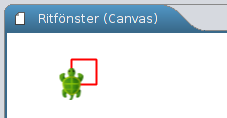
\includegraphics[width=0.47\textwidth]{../img/kojo/kvadrat}

\noindent Prova gärna olika sätt att skriva din kod \emph{utan} att resultatet ändras: skriv satser i sekvens på flera rader eller satser i sekvens på samma rad med semikolon emellan; använd blanktecken och blanka rader i koden. Hur vill du gruppera dina satser så att de är lätta för en människa att läsa?
%Prova att ändra på \emph{ordningen} mellan satserna och studera hur resultatet påverkas. Använd den \emph{gula} play-knappen  (programspårning) för att studera exekveringen i detalj. Vad händer du klickar på satser i ditt program och på rutor i programspårningen?


\Subtask Rita en trappa enligt bilden nedan.

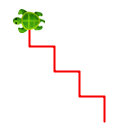
\includegraphics[width=0.3\textwidth]{../img/kojo/stairs}

\Subtask Rita valfri bild på valfri bakgrund med hjälp av några av procedurerna i tabellen nedan. Du kan till exempel rita en rosa triangel med lila konturer mot svart bakgrund. % \ref{lab:kojo:kojo-procedures}.
Försök att underlätta läsbarheten av din kod med hjälp av lämpliga radbrytningar och gruppering av satser.


\begin{table}[H]
\begin{longtable}{l l}\small
\code|fram(100)| & Paddan går framåt 100 steg (25 om argument saknas).\\
\code|färg(rosa)| & Sätter pennans färg till rosa. \\
\code|fyll(lila)| & Sätter ifyllnadsfärgen till lila. \\
\code|fyll(genomskinlig)| & Gör så att paddan \emph{inte} fyller i något när den ritar. \\
\code|bredd(20)| & Gör så att pennan får bredden 20. \\
\code|bakgrund(svart)| & Bakgrundsfärgen blir svart. \\
\code|bakgrund2(grön,gul)| & Bakgrund med övergång från grönt till gult. \\
\code|pennaNer|  & Sätter ner paddans penna så att den ritar när den går. \\
\code|pennaUpp|  & Sänker paddans penna så att den \emph{inte} ritar när den går. \\
\code|höger(45)|   & Paddan vrider sig 45 grader åt höger. \\
\code|vänster(45)| & Paddan vrider sig 45 grader åt vänster. \\
\code|hoppa|       & Paddan hoppar 25 steg utan att rita. \\
\code|hoppa(100)|  & Paddan hoppar 100 steg utan att rita. \\
\code|hoppaTill(100, 200)| & Paddan hoppar till läget (100, 200) utan att rita. \\
\code|gåTill(100, 200)|    & Paddan vrider sig och går till läget (100, 200). \\
\code|öster|   & Paddan vrider sig så att nosen pekar åt höger. \\
\code|väster|  & Paddan vrider sig så att nosen pekar åt vänster. \\
\code|norr|    & Paddan vrider sig så att nosen pekar uppåt. \\
\code|söder|   & Paddan vrider sig så att nosen pekar neråt. \\
\code|mot(100,200)|   & Paddan vrider sig så att nosen pekar mot läget (100, 200) \\
\code|sättVinkel(90)| & Paddan vrider nosen till vinkeln 90 grader. \\
\end{longtable}
%\label{lab:kojo:kojo-procedures}
%\caption{Några användbara procedurer i Kojo.}
\end{table}

\begin{framed}
\noindent\emph{Tips inför fortsättningen:} Ha gärna både REPL och Kojo igång samtidigt. Då kan du undersöka hur olika kodkonstruktioner fungerar i REPL, medan du stegvis skapar allt större program i editorn i Kojo. Detta sätt att jobba har du nytta av under resten av kursen, både om du använder en texteditor och kompilerar i terminalen, och om du använder en professionell integrerad utvecklingsmiljö. Oavsett vilka andra verktyg du kör är det användbart att ha REPL igång i ett eget fönster som hjälp i den kreativa processen, medan du jagar buggar och medan du lär dig nya koncept. Så fort du undrar hur något fungerar i Scala: fram med REPL och testa!
\end{framed}


\SOLUTION

\TaskSolved \what

\SubtaskSolved Genom att börja din Kojo-program med \code{sudda} så startar du exekveringen i samma utgångsläge: en tom rityta \Eng{canvas} där paddan pekar uppåt, pennan är nere och pennans färg är röd.  Då blir det lättare att resonera om vad programmet gör från början till slut, jämfört med om exekveringen beror på resultatet av tidigare exekveringar.


\SubtaskSolved
\begin{Code}
sudda

fram; vänster
fram; vänster
fram; vänster
fram; vänster
\end{Code}


\SubtaskSolved
\begin{Code}
sudda

fram; vänster
fram; höger

fram; vänster
fram; höger

fram; vänster
fram; höger

fram; vänster
\end{Code}


\QUESTEND









\clearpage

\ExtraTasks %%%%%%%%%%%%%%%%%% EXTRAUPPGIFTER



\WHAT{Typ och värde.}

\QUESTBEGIN

\Task \what~Vilket värde och vilken typ hör till vilket uttryck?  Är du osäker på svaret, testa i REPL.

\begin{ConceptConnections}[0.3\textwidth]
  \code|1.0 + 18          | & 1 & & A & \code|42.0: Double    | \\ 
  \code|(41 + 1).toDouble | & 2 & & B & \code|65: Int         | \\ 
  \code|1.042e42 + 1      | & 3 & & C & \code|19.0: Double    | \\ 
  \code|12E6.toLong       | & 4 & & D & \code|12000000: Long  | \\ 
  \code|32.toChar.toString| & 5 & & E & \code|'*': Char       | \\ 
  \code|'A'.toInt         | & 6 & & F & \code|48: Int         | \\ 
  \code|0.toInt           | & 7 & & G & \code|" ": String   | \\ 
  \code|'0'.toInt         | & 8 & & H & \code|1.042E42: Double| \\ 
  \code|'9'.toInt         | & 9 & & I & \code|'q': Char       | \\ 
  \code|'A' + '0'         | & 10 & & J & \code|113: Int        | \\ 
  \code|('A' + '0').toChar| & 11 & & K & \code|0: Int          | \\ 
  \code|"*!%#".charAt(0)| & 12 & & L & \code|57: Int         | \\ 
\end{ConceptConnections}

\SOLUTION

\TaskSolved \what

\begin{ConceptConnections}
  \code|1.0 + 18          | & 1 & ~~\Large$\leadsto$~~ &  E & \code|19.0: Double    | \\ 
  \code|(41 + 1).toDouble | & 2 & ~~\Large$\leadsto$~~ &  L & \code|42.0: Double    | \\ 
  \code|1.042e42 + 1      | & 3 & ~~\Large$\leadsto$~~ &  A & \code|1.042E42: Double| \\ 
  \code|12E6.toLong       | & 4 & ~~\Large$\leadsto$~~ &  K & \code|12000000: Long  | \\ 
  \code|32.toChar.toString| & 5 & ~~\Large$\leadsto$~~ &  G & \code|" ": String   | \\ 
  \code|'A'.toInt         | & 6 & ~~\Large$\leadsto$~~ &  H & \code|65: Int         | \\ 
  \code|0.toInt           | & 7 & ~~\Large$\leadsto$~~ &  I & \code|0: Int          | \\ 
  \code|'0'.toInt         | & 8 & ~~\Large$\leadsto$~~ &  F & \code|48: Int         | \\ 
  \code|'9'.toInt         | & 9 & ~~\Large$\leadsto$~~ &  D & \code|57: Int         | \\ 
  \code|'A' + '0'         | & 10 & ~~\Large$\leadsto$~~ &  B & \code|113: Int        | \\ 
  \code|('A' + '0').toChar| & 11 & ~~\Large$\leadsto$~~ &  J & \code|'q': Char       | \\ 
  \code|"*!%#".charAt(0)| & 12 & ~~\Large$\leadsto$~~ &  C & \code|'*': Char       | \\ 
\end{ConceptConnections}

%\Subtask \code{1.0 + 18}
%
%\Subtask \code{(41 + 1).toDouble}
%
%\Subtask \code{1.042e42 + 1}
%
%\Subtask \code{12E6.toLong}
%
%\Subtask \code{"gurk" + 'a'}
%
%\Subtask \code{32.toChar.toString}
%
%\Subtask \code{'A'.toInt}
%
%\Subtask \linebreak[0] \code{'0'.toInt}
%
%\Subtask \code{'0'.toInt}
%
%\Subtask \code{'9'.toInt}
%
%\Subtask \code{'A' + '0'}
%
%\Subtask \code{('A' + '0').toChar}
%
%\Subtask \code{"*!%#".charAt(0)}
%%%%%%%%%%%%%%%%%%%%%%%%%%%%%%%%%%%%%%%%%%%%%%%%
%\SubtaskSolved \code{Double, 19}
%
%\SubtaskSolved \code{Double, 42}
%
%\SubtaskSolved \code{Double, 1.042E42}
%
%\SubtaskSolved \code{Long, 12000000}
%
%\SubtaskSolved \code{String, gurka}
%
%\SubtaskSolved \code{String, " "}
%
%\SubtaskSolved \code{Int, 65}
%
%\SubtaskSolved \code{Int, 48}
%
%\SubtaskSolved \code{Int,49}
%
%\SubtaskSolved \code{Int,57}
%
%\SubtaskSolved \code{Int, 113}
%
%\SubtaskSolved \code{Char, 'q'}
%
%\SubtaskSolved \code{Char, '*'}


\QUESTEND




\WHAT{Satser och uttryck.}

\QUESTBEGIN

\Task \what

\Subtask Vad är det för skillnad på en sats och ett uttryck?

\Subtask Ge exempel på satser som inte är uttryck?

\Subtask Förklara vad som händer för varje evaluerad rad:
\begin{REPL}
scala> def värdeSaknas = ()
scala> värdeSaknas
scala> värdeSaknas.toString
scala> println(värdeSaknas)
scala> println(println("hej"))
\end{REPL}

\Subtask Vilken typ har literalen \code{()}?

\Subtask Vilken returtyp har \code{println}?

\SOLUTION

\TaskSolved \what

\SubtaskSolved  Ett utryck kan evalueras och resulterar då i ett användbart värde. En sats \emph{gör} något (t.ex. skriver ut något), men resulterat inte i något användbart värde.

\SubtaskSolved \code{println()}

\SubtaskSolved

 \code{värdeSaknas} innehåller Unit

 Skriver ut \code{Unit}

 Skriver ut \code{"()"}

 Skriver ut \code{"()"}

 Skriver först ut hej med det innersta anropet och sen \code{()} med det yttre anropet

\SubtaskSolved  \code{Unit}

\SubtaskSolved  \code{Unit}

\QUESTEND



\WHAT{Procedur med parameter.}

\QUESTBEGIN

\Task \what~En procedur är en funktion som orsakar en effekt, till exempel en utskrift eller en variabeltilldelning, men som inte returnerar något intressant resultatvärde.%
\footnote{I Scala är procedurer funktioner som returnerar det \emph{tomma värdet}, vilket skrivs \code{()} och är av typen \code{Unit}. I Java och flera andra språk finns inget tomt värde och man har en specialsyntax för procedurer som använder nyckelordet \code{void}. }

\Subtask Deklarera en förändringsbar variabel \code{highscore} som initieras till 0.

\Subtask Deklarera en procedur \code{updateHighscore} som tar en parameter \code{points} och tilldelar \code{highscore} ett nytt värde om \code{points} är större än \code{highscore} och skriver ut strängen \code{"REKORD!"}. Om inte \code{points} är större än \code{highscore} ska strängen \code{"GE INTE UPP!"} skrivas ut. Testa proceduren i REPL.

\Subtask Gör en ny variant av \code{updateHighscore}, som \emph{inte} är en procedur utan i stället är en funktion som ger en sträng för senare utskrift. Testa funktionen i REPL.

\SOLUTION

\TaskSolved \what

\SubtaskSolved
\begin{Code}
var highscore = 0
\end{Code}

\SubtaskSolved
\begin{Code}
def updateHighscore(points: Int): Unit =
  if points > highscore then
    highscore = points
    println("REKORD!")
  else println("GE INTE UPP!")
\end{Code}

\SubtaskSolved
\begin{Code}
def updateHighscore(points: Int): String =
  if points > highscore then
    highscore = points
    "REKORD!"
  else "GE INTE UPP!"
\end{Code}



\QUESTEND


\WHAT{Flyttalsaritmetik.}

\QUESTBEGIN

\Task \what

\Subtask Vilket är det minsta positiva värdet av typen \code{Double}?

\Subtask Vad är värdet av detta uttryck? Varför blir det så?
\begin{REPL}
scala> Double.MaxValue + Double.MinPositiveValue == Double.MaxValue
\end{REPL}

\SOLUTION

\TaskSolved \what

\SubtaskSolved

\begin{REPL}
scala> Double.MinPositiveValue
res0: Double = 4.9E-324
\end{REPL}

\SubtaskSolved

\begin{REPL}
scala> Double.MaxValue + Double.MinPositiveValue == Double.MaxValue
res2: Boolean = true
\end{REPL}

\QUESTEND



\WHAT{\code{if}\textit{-sats}.}

\QUESTBEGIN

\Task \what~För varje rad nedan, beskriv vad som skrivs ut.  % Uppgift 18
\begin{REPL}
scala> if !true then println("sant") else println("falskt")
scala> if !false then println("sant") else println("falskt")
scala> def singlaSlant = if math.random() < 0.5 then "krona" else "klave"
scala> for i <- 1 to 5 do print(s"$i:$singlaSlant ")
\end{REPL}

\SOLUTION

\TaskSolved \what

\begin{enumerate}
\item Utskrift: \code{falskt}
\item Utskrift: \code{sant}
\item Inget skrivs ut, funktionen deklareras men körs ej.
\item Utskrift: \code{1:krona 2:klave 3:krona 4:krona 5:klave } eller liknande beroende på vilka slumptal \code{math.random()} ger.
\end{enumerate}

\QUESTEND




\WHAT{\code{if}\textit{-uttryck}.}

\QUESTBEGIN

\Task  Deklarera följande variabler med nedan initialvärden:

\begin{REPLnonum}
scala> var grönsak = "gurka"
scala> var frukt = "banan"
\end{REPLnonum}

Ange för varje rad nedan vad uttrycket har för värde och typ:
\begin{REPLnonum}
scala> if grönsak == "tomat" then "gott" else "inte gott"
scala> if frukt == "banan" then "gott" else "inte gott"
scala> if true then grönsak else 42
scala> if false then grönsak else 42
\end{REPLnonum}

\SOLUTION


\TaskSolved \what~Notera typen \code{Any} på de sista två uttrycken.

\begin{REPLnonum}
scala> if grönsak == "tomat" then "gott" else "inte gott"
res0: String = inte gott

scala> if frukt == "banan" then "gott" else "inte gott"
res1: String = gott

scala> if true then grönsak else 42
res2: Any = gurka

scala> if false then grönsak else 42
res3: Any = 42
\end{REPLnonum}


\QUESTEND





\WHAT{Modulo-operatorn {\tt \%} och Booleska värden.}

\QUESTBEGIN

\Task \what

\Subtask Deklarera en funktion \code{def isEven(n: Int): Boolean = ???} som ger \code{true} om talet \code{n} är jämnt, annars \code{false}.

\Subtask Deklarera en funktion \code{def isOdd(n: Int): Boolean = ???} som ger \code{false} om talet \code{n} är jämnt, annars \code{true}.

\SOLUTION


\TaskSolved \what

\SubtaskSolved
\begin{REPL}
scala> def isEven(n: Int): Boolean = n % 2 == 0

scala> isEven(42)
res0: Boolean = true

scala> isEven(43)
res1: Boolean = false

\end{REPL}


\SubtaskSolved
\begin{REPL}
scala> def isOdd(n: Int): Boolean = !isEven(n)

scala> isOdd(42)
res2: Boolean = false

scala> isOdd(43)
res3: Boolean = true
\end{REPL}


\QUESTEND





\WHAT{Skillnader mellan \code{var}, \code{val}, \code{def}.}

\QUESTBEGIN

\Task \what~

\Subtask
 Evaluera varje rad en i taget i tur och ordning i Scala REPL. För varje rad nedan: förklara för vad som händer och notera värde och ev fel. % Uppgift 15
\begin{REPL}
scala> var x = 30
scala> x + 1
scala> x = x + 1
scala> x == x + 1
scala> val y = 20
scala> y = y + 1
scala> var z = { println("hej z!"); math.random() }
scala> def w = { println("hej w!"); math.random() }
scala> z
scala> z
scala> z = z + 1
scala> w
scala> w
scala> w = w + 1
\end{REPL}


\Subtask Vad är det för skillnad på \code{var}, \code{val} och \code{def}?



\SOLUTION

\TaskSolved \what

\SubtaskSolved
\begin{REPL}
  scala> var x = 30
  x: Int = 30

  scala> x + 1
  res6: Int = 31

  scala> x = x + 1
  x: Int = 31

  scala> x == x + 1
  res7: Boolean = false

  scala> val y = 20
  y: Int = 20

  scala> y = y + 1
  <console>:12: error: reassignment to val
         y = y + 1
           ^

  scala> var z = { println("hej z!"); math.random() }
  hej z!
  z: Double = 0.3381365875903367

  scala> def w = { println("hej w!"); math.random() }
  w: Double

  scala> z
  res8: Double = 0.3381365875903367

  scala> z
  res9: Double = 0.3381365875903367

  scala> z = z + 1
  z: Double = 1.3381365875903368

  scala> w
  hej w!
  res10: Double = 0.06420209879434557

  scala> w
  hej w!
  res11: Double = 0.5777951341051852

  scala> w = w + 1
  <console>:12: error: value w_= is not a member of object
         w = w + 1
\end{REPL}


\SubtaskSolved
\begin{itemize}
\item \code{var namn = uttryck} används för att deklarera en förändringsbar variabel. Namnet kan med hjälp av en tilldelningssats referera till nya värden.

\item \code{val namn = uttryck} används för att deklarera en oföränderlig variabel som efter initialisering inte kan förändras med tilldelningssatser. Vid försök ges kompileringsfel.
\item \code{def namn = uttryck} används för att deklarera en funktion vars uttryck evalueras varje gång den anropas.
\end{itemize}

\QUESTEND




\WHAT{Skillnaden mellan \code{if} och \code{while}.}

\QUESTBEGIN

\Task \what~Vad blir resultatet av rad 3 och 4?

\begin{REPL}
scala> def lotto1 = if math.random() > 0.5 then print("vinst :) ")
scala> def lotto2 = while math.random() > 0.5 do print("vinst :) ")
scala> lotto1
scala> lotto2
\end{REPL}

\SOLUTION

\TaskSolved \what

\begin{itemize}
\item Rad 3: Har du tur (50\% chans) får du vinst en gång.

\item Rad 4: Har du tur får du många vinster i rad. Sannolikheten för $n$ vinster i rad är $(\frac{1}{2})^n$.
\end{itemize}
\QUESTEND












\clearpage

\AdvancedTasks   %%%%%%%%%%%%%%%%%%% FÖRDJUPNINGSUPPGIFTER





\WHAT{Logik och De Morgans Lagar.}

\QUESTBEGIN

\Task \what~Förenkla följande uttryck. Antag att \code{poäng} och \code{highscore} är heltalsvariabler medan \code{klar} är av typen \code{Boolean}.
  % Uppgift 24

\Subtask \code{poäng > 100 && poäng > 1000}

\Subtask \code{poäng > 100 || poäng > 1000}

\Subtask \code{!(poäng > highscore)}

\Subtask \code{!(poäng > 0 && poäng < highscore) }

\Subtask \code{!(poäng < 0 || poäng > highscore) }

\Subtask \code{klar == true}

\Subtask \code{klar == false}

\SOLUTION

\TaskSolved \what


\SubtaskSolved \code{poäng > 1000}

\SubtaskSolved \code{poäng > 100}

\SubtaskSolved \code{poäng <= highscore}

\SubtaskSolved \code{poäng <= 0 || poäng >= highscore }

\SubtaskSolved \code{poäng >= 0 && poäng <= highscore}

\SubtaskSolved \code{klar}

\SubtaskSolved \code{!klar}


\QUESTEND






\WHAT{Stränginterpolatorn \code{s}.}

\QUESTBEGIN

\Task \what~Med ett \code{s} framför en strängliteral får man hjälp av kompilatorn att, på ett typsäkert sätt, infoga variabelvärden i en sträng.
Variablernas namn ska föregås med ett dollartecken , t.ex. \code{s"Hej $namn"}.
Om man vill evaluera ett uttryck placeras detta inom klammer direkt efter dollartecknet, t.ex.
\code/s"Dubbla längden: ${namn.size * 2}"/

\Subtask Vad skrivs ut nedan?
\begin{REPL}
scala> val f = "Kim"
scala> val e = "Finkodare"
scala> println(s"Namnet '$f $e' har ${f.size + e.size} bokstäver.")
\end{REPL}

\Subtask Skapa följande utskrifter med hjälp av stränginterpolatorn \code{s} och variablerna \code{f} och \code{e} i föregående deluppgift.
\begin{REPL}
Kim har 3 bokstäver.
Finkodare har 9 bokstäver.
\end{REPL}

\SOLUTION

\TaskSolved \what

\SubtaskSolved
\begin{REPLnonum}
Namnet 'Kim Finkodare' har 12 bokstäver.
\end{REPLnonum}

\SubtaskSolved
\begin{REPLnonum}
println(s"$f har  ${f.size} bokstäver.")
println(s"$e har  ${e.size} bokstäver.")
\end{REPLnonum}

\QUESTEND



\WHAT{Tilldelningsoperatorer.}

\QUESTBEGIN

\Task \what~Man kan förkorta en tilldelningssats som förändrar en variabel, t.ex. \code{x = x + 1}, genom att använda så kallade tilldelningsoperatorer och skriva \code{x += 1} som betyder samma sak. Rita en ny bild av datorns minne efter varje rad nedan. Bilderna ska visa variablers namn, typ och värde.

\begin{REPL}
scala> var a = 40
scala> var b = a + 40
scala> a += 10
scala> b -= 10
scala> a *= 2
scala> b /= 2
\end{REPL}

\SOLUTION

\TaskSolved \what

\begin{tabular}{l l}
\MEM{{\it Efter rad1:~~~~} a}{Int}{40}\\
\MEM{{\it Efter rad2:~~~~} a}{Int}{40} & \MEM{b}{Int}{80}\\
\MEM{{\it Efter rad3:~~~~} a}{Int}{50} & \MEM{b}{Int}{80}\\
\MEM{{\it Efter rad4:~~~~} a}{Int}{50} & \MEM{b}{Int}{70} \\
\MEM{{\it Efter rad5:~~~~} a}{Int}{100} & \MEM{b}{Int}{70} \\
\MEM{{\it Efter rad6:~~~~} a}{Int}{100} & \MEM{b}{Int}{35} \\
\end{tabular}

\QUESTEND






\WHAT{Stora tal.}

\QUESTBEGIN

\Task \what~Om vi vill beräkna $2^{64} -1$ som ett exakt heltal\footnote{\url{https://en.wikipedia.org/wiki/Wheat_and_chessboard_problem}} blir det större än \code{Int.MaxValue}, så vi kan tyvärr inte använda snabba \code{Int}. Till vår räddning: \code{BigInt}

\Subtask Läs om \code{BigInt} och \code{BigDecimal} på \Scaladoc \\ Notera vad de kan användas till.

\Subtask Du skapar ett \code{BigInt}-heltal med \code{BigInt(2)} och kan anropa funktionen \code{pow} på en \code{BigInt} med punktnotation. Beräkna $2^{64} -1$ som ett exakt heltal.

\Subtask Vilka nackdelar finns med \code{BigInt} och \code{BigDecimal}?

\SOLUTION

\TaskSolved \what

\SubtaskSolved \code{BigInt} kan användas i stället för \code{Int} vid mycket stora heltal. Det finns förståss även \code{Long} som har dubbelt omfång jämfört med \code{Int}, medan \code{BigInt} kan ha godtyckligt många siffror (ända tills minnet tar slut) och kan därmed representera ofantligt stora tal. \code{BigDecimal} kan användas i stället för \code{Double} vid mycket stora decimaltal.

\SubtaskSolved
\begin{REPL}
scala> BigInt(2).pow(64)
res0: scala.math.BigInt = 18446744073709551616
\end{REPL}

\SubtaskSolved Beräkningar går mycket långsammare och de är lite krångligare att använda.

\QUESTEND





\WHAT{Precedensregler}

\QUESTBEGIN

\Task \what~Evalueringsordningen kan styras med parenteser. Vilket värde och vilken typ har följande uttryck?

\Subtask \code{23 + 2 * 2 + (23 + 2) * 2}

\Subtask \code{(-(2 - 42)) / (1 + 1 + 1)}

\Subtask \code{(-(2 - 42)) / (-1)/(1 + 1 + 1)}

\SOLUTION

\TaskSolved \what

\SubtaskSolved \code{77:  Int}

\SubtaskSolved \code{13: Int}

\SubtaskSolved \code{-13: Int}

\QUESTEND



\WHAT{Dokumentation av paket i Java och Scala.}

\QUESTBEGIN

\Task \what


\Subtask Genom att trycka på tab tangenten kan man se vad som finns i olika paket. Vad heter konstanten $\pi$  i \code{java.lang.Math} (notera stort M) respektive \code{scala.math.}?

\begin{REPL}
scala> java.lang.Math.    //tryck TAB efter punkten
scala> scala.math.        //tryck TAB efter punkten
\end{REPL}

\Subtask Jämför dokumentationen för klassen \code{java.lang.Math} här: \\ \url{https://docs.oracle.com/javase/8/docs/api/} \\
med dokumentationen för paketet \code{scala.math} här: \\
\url{http://www.scala-lang.org/api} \\
Ge exempel på vad man kan göra på webbsidan med Scala-dokumentationen som man \emph{inte} kan göra i motsvarande webbsida Java-dokumentation.

\Subtask Vad gör metoden \code{hypot}? Vad är det som är bra med att använda \code{hypot} i stället för att själv implementera beräkningen med hjälp av kvadratrot, multiplikation och addition?

\SOLUTION

\TaskSolved \what

\SubtaskSolved Scala: \code{Pi}, Java: \code{PI}

\SubtaskSolved Man kan söka och filtrera fram alla förekomster av en viss teckenkombination.

\SubtaskSolved Räknar ut hypotenusan (Pythagoras sats) utan risk för avrundningsproblem i mellanberäkningar.


\QUESTEND





\WHAT{Noggrannhet och undantag i aritmetiska uttryck.}

\QUESTBEGIN

\Task \what~Vad blir resultatet av uttrycken nedan? Notera undantag \Eng{exceptions} och noggrannhetsproblem.

\Subtask \code{Int.MaxValue + 1}

\Subtask \code{1 / 0}

\Subtask \code{1E8 + 1E-8}

\Subtask \code{1E9 + 1E-9}

\Subtask \code{math.pow(math.hypot(3,6), 2)}

\Subtask\Uberkurs \code{1.0 / 0}

\Subtask\Uberkurs \code{(1.0 / 0).toInt}

\Subtask\Uberkurs \code{math.sqrt(-1)}

\Subtask\Uberkurs \code{math.sqrt(Double.NaN)}

\Subtask \code{throw new Exception("PANG!!!")}

\SOLUTION

\TaskSolved \what

\SubtaskSolved \code{-2147483648} vilket motsvarar \code{Int.MinValue}.

\SubtaskSolved Ett undantag kastas: \code{java.lang.ArithmeticException: / by zero}

\SubtaskSolved \code{1.0000000000000001E8} (som förväntat)

\SubtaskSolved Avrundas till \code{1E9} (flyttalsaritmetik med noggrannhetsproblem: ett stort flyttal plus ett (alltför) litet flyttal kan ge samma tal. Det lilla talet ''försvinner'').


\SubtaskSolved \code{45.00000000000001} (flyttalsaritmetik med noggrannhetsproblem: enligt ''normal'' aritmetik ska det bli exakt 45.)

\SubtaskSolved \code{Infinity} (som även ges av \code{Double.PositiveInfinity} och som representerar den positiva oändligheten).

\SubtaskSolved \code{2147483647} vilket motsvarar \code{Int.MaxValue}.

\SubtaskSolved \code{NaN} vilket betyder ''Not a Number''.

\SubtaskSolved \code{NaN} vilket betyder ''Not a Number''.

\SubtaskSolved Ett undantag kastas: \code{java.lang.Exception: PANG!!!}

\QUESTEND



\WHAT{Modulo-räkning med negativa tal.}

\QUESTBEGIN

\Task\Uberkurs \what~Läs om moduloräkning här: \\
 \href{https://en.wikipedia.org/wiki/Modulo\_operation}{en.wikipedia.org/wiki/Modulo\_operation} \\
 och undersök hur det blir med olika tecken (positivt resp. negativt) på moduloräkning med $dividend \% divisor$ i Scala.


\SOLUTION

\TaskSolved \what~I Scala har resultatet samma tecken som dividenden.
\begin{REPL}
scala> 1 % 2
res0: Int = 1

scala> -1 % 2
res1: Int = -1

scala> -1 % -2
res2: Int = -1

scala> 1 % -2
res3: Int = 1

\end{REPL}

\QUESTEND




\WHAT{Bokstavliga identifierare.}

\QUESTBEGIN

\Task\Uberkurs \what~Läs om identifierare i Scala och speciellt \emph{literal identifiers} här: \url{http://www.artima.com/pins1ed/functional-objects.html#6.10}.

\Subtask Förklara vad som händer nedan:
\begin{REPLnonum}
scala> val `bokstavlig val` = 42
scala> println(`bokstavlig val`)
\end{REPLnonum}

\Subtask Scala och Java har olika uppsättningar med reserverade ord. På vilket sätt kan ''backticks'' vara använbart med anledning av detta?

\SOLUTION

\TaskSolved \what

\SubtaskSolved Variabeln får namnet 'bokstavlig val', bakåt-apostrofer \Eng{backticks} gör att man kan namnge variabler till annars otillåtna namn, t.ex. med mellanrum eller nyckelord i sig.

\SubtaskSolved Backticks i Scala möjliggör alla möjliga tecken i namn. Exempel på användning: I java finns en metod som heter \jcode{java.lang.Thread.yield} men i Scala är yield ett nyckelord; för att komma runt det går det att i Scala skriva \jcode{java.lang.Thread.`yield`}

\QUESTEND












\WHAT{\code{java.lang.Integer}, hexadecimala litteraler, BigDecimal.}

\QUESTBEGIN

\Task\Uberkurs \what~

\Subtask Sök upp dokumentationen för \code{java.lang.Integer}.\\Använd metoderna \code{toBinaryString} och \code{toHexString} för att fylla i tabellen nedan.

\begin{table}[H]
\begin{tabular}{l | l | l}
decimalt heltal & binärt värde & hexadecimalt värde \\
\hline
$33$ &   &  \\
$42$ &   &  \\
$64$ &   &  \\
\end{tabular}
\end{table}

\Subtask Hur anger man det hexadecimala heltalsvärdet 10c (motsvarar 268 decimalt) som en litteral i Scala?

\Subtask Vad blir \code{0x10} upphöjt till $c =$ ljusets hastighet i $m/s$? \emph{Tips:} Använd \code{BigDecimal}.

\SOLUTION

\TaskSolved \what

\SubtaskSolved

\begin{REPL}
scala> import Integer.{toBinaryString => toBin, toHexString => toHex}

scala> for i <- Seq(33, 42, 64) do println(s"$i \t ${toBin(i)} \t ${toHex(i)}")
33 	 100001 	 21
42 	 101010 	 2a
64 	 1000000 	 40
\end{REPL}


\SubtaskSolved Det hexadecimala heltalet $10c$ kan anges med litteralen \code{0x10c} i Scala, Java och många andra språk: \footnote{\url{https://en.wikipedia.org/wiki/0x10c}}
\begin{REPL}
scala> 0x10c
res0: Int = 268
\end{REPL}

\SubtaskSolved \footnote{\url{https://c418.bandcamp.com/album/0x10c}}
\begin{REPL}
scala> val c = 299792458
c: Int = 299792458

scala> BigDecimal(0x10).pow(c)
res68: scala.math.BigDecimal = 2.124892963227906613060986110887672E+360986089
\end{REPL}


\QUESTEND









\WHAT{Strängformatering.}

\QUESTBEGIN

\Task\Uberkurs \what~Läs om \code{f}-interpolatorn här:\\
\url{http://docs.scala-lang.org/overviews/core/string-interpolation.html} \\
Hur kan du använda \code{f}-interpolatorn för att göra följande utskrift i REPL? Ändra rad 3 vid \code{???} så att flyttalet \code{g} avrundas till tre decimaler innan utskrift sker.
\begin{REPL}
scala> val g = 2 / 3.0
scala> val str = f"Jättegurkan är $g??? meter lång"
scala> println(str)
Jättegurkan är 0.667 meter lång
\end{REPL}

\SOLUTION

\TaskSolved \what

\begin{Code}
val str = f"Jättegurkan är $g%1.3f meter lång"
\end{Code}
(Om du tycker att \code{$g%1.3f}
ser kryptiskt ut, så kan du trösta dig med att du nu får chansen att föra vidare ett anrikt arv från det urgamla språket C och den sägenomspunna funktionen \code{printf} till kommande generationer av invigda kodmagiker.)

\QUESTEND




\WHAT{Multiplikationsvarning.}

\QUESTBEGIN

\Task \what~Sök upp dokumentationtionen för\\\code{java.lang.Math.multiplyExact} och läs om vad den metoden gör.

\Subtask Vad händer här?

\begin{REPLnonum}
scala> Math.multiplyExact(1, 2)
scala> Int.MaxValue * 2
scala> Math.multiplyExact(Int.MaxValue, 2)
\end{REPLnonum}

\Subtask Varför kan man vilja använda \code{java.lang.Math.multiplyExact} i stället för ''vanlig'' multiplikation?

\SOLUTION

\TaskSolved \what

\SubtaskSolved Den andra multiplikationen flödar över \Eng{overflow} gränsen för största möjliga värdet av en \code{Int}. I den tredje multiplikationen kastas i stället ett undantag \code{java.lang.ArithmeticException: integer overflow}


\begin{REPLnonum}
scala> Math.multiplyExact(1, 2)
res70: Int = 2

scala> Int.MaxValue * 2
res71: Int = -2

scala> Math.multiplyExact(Int.MaxValue, 2)
java.lang.ArithmeticException: integer overflow
  at java.lang.Math.multiplyExact(Math.java:867)
  ... 42 elided
\end{REPLnonum}

\SubtaskSolved Används då man vill vara helt säker på att overflow-buggar ''smäller'' direkt i stället för att generera felaktiga resultat vars konsekvenser kanske manifesterar sig långt senare. Dock är \code{multiplyExact} aningen långsammare än vanlig multiplikation.


\QUESTEND








\WHAT{Dekorera \code{Int} med extra operatorer.}

\QUESTBEGIN

\Task\Uberkurs \what\footnote{En utmanande överkursuppgift som visar Scalas kraftfullhet. Se fördjupningslänkar i facit.}\\Kim Kodmagiker tycker att \code{Math.multiplyExact} är för krångligt att skriva och utökar därför typen \code{Int} med en extra operator:

\begin{Code}
implicit class IntDecorator(val i: Int) extends AnyVal {
  def *!(j: Int) = Math.multiplyExact(i,j)
}
\end{Code}

\Subtask Klistra in koden ovan i REPL och prova den extra operatorn.

\Subtask Hjälp Kim Kodmagiker att lägga till fler operatorer på värden av typen \code{Int}, som gör att det även går att använda \code{Math.subtractExact} och \code{Math.addExact} smidigt.

\Subtask Testa ett sammansatt uttryck som använder alla extrametoder på \code{Int}. Tycker du det blev mer lättläst eller mer kryptiskt med de nya operatorerna?

\SOLUTION

\TaskSolved \what

\SubtaskSolved

\begin{REPL}
scala> Int.MaxValue *! 1
res0: Int = 2147483647

scala> Int.MaxValue *! 2
java.lang.ArithmeticException: integer overflow
  at java.lang.Math.multiplyExact(Math.java:867)
  at IntExtra.$times$bang(<console>:16)
  ... 32 elided

\end{REPL}

Kort förklaring:
\begin{itemize}
\item \code{implicit class MinDekorator(x: Typ)} gör så att operationer i dekoratorklassen \code{MinDekorator} automatiskt görs tillgängliga på värden av typen \code{Typ}.%
\footnote{Fördjupning: \url{http://docs.scala-lang.org/overviews/core/implicit-classes.html}}

\item \code{extends AnyVal} gör så att kompilatorn försöker generera maskinkod som blir lika effektiv som vid direkt användning av det underliggande värdet.%
\footnote{Fördjupning: \url{http://docs.scala-lang.org/overviews/core/value-classes.html}}
\end{itemize}


\SubtaskSolved

\begin{Code}
implicit class IntDecorator(val i: Int) extends AnyVal{
  def *!(j: Int) = Math.multiplyExact(i,j)
  def +!(j: Int) = Math.addExact(i,j)
  def -!(j: Int) = Math.subtractExact(i,j)
}
\end{Code}


\SubtaskSolved Det blir lätt väldigt kryptiskt med namn som består av flera specialtecken. Om du \emph{verkligen} vill ha sådana operatorer är det \emph{mycket} lämpligt att också erbjuda varianter i klartext:
\begin{Code}
implicit class IntDecorator(val i: Int) extends AnyVal{
  def mulExact(j: Int) = Math.multiplyExact(i,j)
  def *!(j: Int) = i mulExact j

  def addExact(j: Int) = Math.addExact(i,j)
  def +!(j: Int) = i addExact j

  def subExact(j: Int) = Math.subtractExact(i,j)
  def -!(j: Int) = i subExact j
}

\end{Code}


\QUESTEND



%%%%%%%%%%%%%%%%%%%%%%%%%%%%%%%%%%%%%%%%%%%%%%%%
%%%%%%%%%%%%%%%%%%%%%%%%%%%%%%%%%%%%%%%%%%%%%%%%
%%%%%%%%%%%%%%%%%%%%%%%%%%%%%%%%%%%%%%%%%%%%%%%%
%%%%%%%%%%%%%%%%%%%%%%%%%%%%%%%%%%%%%%%%%%%%%%%%
%%%%%%%%%%%%%%%%%%%%%%%%%%%%%%%%%%%%%%%%%%%%%%%%
%%%%%%%%%%%%%%%%%%%%%%%%%%%%%%%%%%%%%%%%%%%%%%%%
%%%%%%%%%%%%%%%%%%%%%%%%%%%%%%%%%%%%%%%%%%%%%%%%
%%%%%%%%%%%%%%%%%%%%%%%%%%%%%%%%%%%%%%%%%%%%%%%%
%%%%%%%%%%%%%%%%%%%%%%%%%%%%%%%%%%%%%%%%%%%%%%%%


%% Saker som inte fick plats:



%\Task Läs om BigInt och BigDecimal här: \href{http://alvinalexander.com/scala/how-to-use-large-integer-decimal-numbers-in-scala-bigint-bigdecimal}{alvinalexander.com/scala/how-to-use-large-integer-decimal-numbers-in-scala-bigint-bigdecimal} och prova att skapa riktigt stora tal med hjälp av metoden \code{pow} på BigInt och tal med riktigt många decimaler med BigDecimal dess metod \code{pow}.


%
%
%\Subtask\Pen Sök med Ctrl+F i webbläsaren och efter förekomster av texten \textit{''overflow''} i javadoc för klassen \code{java.lang.Math} i JDK 8. Vad är ''overflow''? Vilka metoder finns i \code{java.lang.Math} som hjälper dig att upptäcka om det blir overflow?
%
%\Task Använda Scala REPL för att undersöka konstanterna nedan. Vilket av dessa värden är negativt? Vad kan man ha för praktisk nytta av dessa värden i ett program som gör flyttalsberäkningar?
%
%\Subtask \code{java.lang.Double.MIN_VALUE}
%
%\Subtask \code{scala.Double.MinValue}
%
%\Subtask \code{scala.Double.MinPositiveValue}
%
%\Task För typerna \code{Byte}, \code{Short}, \code{Char}, \code{Int}, \code{Long}, \code{Float}, \code{Double}: Undersök hur många bitar som behövs för att representera varje typs omfång? \\*
%\textit{Tips:} Några användbara uttryck: \\*
% \code{Integer.toBinaryString(Int.MaxValue + 1).size} \\*
% \code{Integer.toBinaryString((math.pow(2,16) - 1).toInt).size} \\*
% \code{1 + math.log(Long.MaxValue)/math.log(2)}
%Se även språkspecifikationen för Scala, kapitlet om heltalsliteraler: \\
%\url{http://www.scala-lang.org/files/archive/spec/2.11/01-lexical-syntax.html#integer-literals}
%
%\Subtask Undersök källkoden för paketobjektet \code{scala.math} här: \\
%\url{https://github.com/scala/scala/blob/v2.11.7/src/library/scala/math/package.scala} \\
%Hur många olika överlagrade varianter av funktionen \code{abs} finns det och för vilka parametertyper är den definierad?

%!TEX encoding = UTF-8 Unicode
%!TEX root = ../labs.tex

\Lab{\LabWeekONE}
%\externaldocument{compendium}
\begin{Goals}
%!TEX encoding = UTF-8 Unicode

\item Kunna kombinera principerna sekvens, alternativ, repetition, och abstraktion i skapandet av egna program om minst 20 rader kod.
\item Kunna förklara vad ett program gör i termer av sekvens, alternativ, repetition, och abstraktion.
\item Kunna tillämpa principerna sekvens, alternativ, repetition, och abstraktion i enkla algoritmer.
\item Kunna formatera egna program så att de blir lätta att läsa och förstå.
\item Kunna förklara vad en variabel är och kunna skriva deklarationer och göra tilldelningar.
\item Kunna genomföra upprepade varv i cykeln \emph{editera-exekvera-felsöka/förbättra} för att successivt bygga upp allt mer utvecklade program.

\end{Goals}

\begin{Preparations}
\item Repetera veckans föreläsningsmaterial.
\item \DoExercise{\ExeWeekONE}{01}%Gör övning {\tt \ExeWeekONE} i kapitel \ref{exe:W01}.
\item Läs om Kojo i appendix \ref{appendix:kojo}. Kojo Desktop är förinstallerat på LTH:s datorer; om du vill installera Kojo Desktop på din egen dator, följ instruktionerna i \ref{appendix:ide:kojo:install}. Du kan också köra Kojo i din webbläsare här: \url{http://kojo.lu.se/}
\item Läs igenom hela laborationen nedan. Fundera på möjliga lösningar till de uppgifter som är markerade med en penna i marginalen.
% \item Ladda hem och studera översiktligt detta dokument (25 sidor, det räcker att du bläddrar igenom dokumentet och får en uppfattning om hur Kojo kan användas): \\ ''Introduction to Kojo'' \url{http://www.kogics.net/kojo-ebooks#intro}
\end{Preparations}

\subsection{Obligatoriska uppgifter}

Om det förekommer en penna i marginalen ska du anteckna något inför redovisningen.


%%%%%%%%%%%%%%NEDAN ÄR FLYTTAT TILL ÖVNING 1 FÖR ATT GÖRA TYDLIGARE KOPPLING MELLAN LABBAR OCH ÖVN
%\Task \textit{Sekvens}.
%
%\Subtask Starta Kojo. Om du inte redan har svenska menyer: välj svenska i språkmenyn och starta om Kojo.  Skriv in nedan program och tryck på den \emph{gröna} play-knappen.
%
%\begin{Code}
%sudda
%
%fram; höger
%fram; vänster
%färg(grön)
%fram
%\end{Code}
%\noindent
%%Genom att börja din Kojo-program med \code{sudda} så startar du exekveringen i samma utgångsläge: en tom canvas där paddan pekar uppåt, pennan är nere och pennans färg är röd.
%%Då blir det lättare att resonera om vad programmet gör från början till slut, jämfört med om exekveringen beror på resultatet av tidigare exekveringar.
%
%\Subtask\Pen Vad händer om du \emph{inte} börjar programmet med \code{sudda} och kör samma program upprepade gånger? Varför är det bra att börja programmet med \code{sudda}?
%
%\Subtask Rita en kvadrat enligt bilden nedan.
%\vspace{1em}\\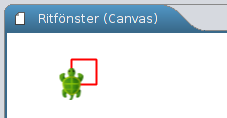
\includegraphics[width=0.45\textwidth]{../img/kojo/kvadrat}
%
%\Subtask Prova olika sätt att skriva din kod \emph{utan} att resultatet ändras: skriv satser i sekvens på flera rader eller satser i sekvens på samma rad med semikolon emellan; använd blanktecken och blanka rader i koden. Hur vill du gruppera dina satser så att de är lätta för en människa att läsa?
%
%\Subtask Prova att ändra på \emph{ordningen} mellan satserna och studera hur resultatet påverkas. Använd den \emph{gula} play-knappen  (programspårning) för att studera exekveringen i detalj. Klicka på satser i ditt program och på rutor i programspårningen och se vad som händer.
%
%
%\Subtask Rita en trappa enligt bilden nedan.
%
%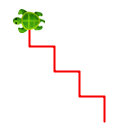
\includegraphics[width=0.2\textwidth]{../img/kojo/stairs}
%
%\Subtask Rita valfri bild på valfri bakgrund med hjälp av några av procedurerna i tabellen nedan. Du kan till exempel rita en rosa triangel med lila konturer mot svart bakgrund. % \ref{lab:kojo:kojo-procedures}.
%Försök att underlätta läsbarheten av din kod med hjälp av lämpliga radbrytningar och gruppering av satser. Undersök hur ordningen av satserna i din kod påverkar resultatet.
%
%
%
%\begin{table}[H]
%\begin{tabular}{l l}\small
%\code|fram(100)| & Paddan går framåt 100 steg (25 om argument saknas).\\
%\code|färg(rosa)| & Sätter pennans färg till rosa. \\
%\code|fyll(lila)| & Sätter ifyllnadsfärgen till lila. \\
%\code|fyll(genomskinlig)| & Gör så att paddan \emph{inte} fyller i något när den ritar. \\
%\code|bredd(20)| & Gör så att pennan får bredden 20. \\
%\code|bakgrund(svart)| & Bakgrundsfärgen blir svart. \\
%\code|bakgrund2(grön,gul)| & Bakgrund med övergång från grönt till gult. \\
%\code|pennaNer|  & Sätter ner paddans penna så att den ritar när den går. \\
%\code|pennaUpp|  & Sänker paddans penna så att den \emph{inte} ritar när den går. \\
%\code|höger(45)|   & Paddan vrider sig 45 grader åt höger. \\
%\code|vänster(45)| & Paddan vrider sig 45 grader åt vänster. \\
%\code|hoppa|       & Paddan hoppar 25 steg utan att rita. \\
%\code|hoppa(100)|  & Paddan hoppar 100 steg utan att rita. \\
%\code|hoppaTill(100, 200)| & Paddan hoppar till läget (100, 200) utan att rita. \\
%\code|gåTill(100, 200)|    & Paddan vrider sig och går till läget (100, 200). \\
%\code|öster|   & Paddan vrider sig så att nosen pekar åt höger. \\
%\code|väster|  & Paddan vrider sig så att nosen pekar åt vänster. \\
%\code|norr|    & Paddan vrider sig så att nosen pekar uppåt. \\
%\code|söder|   & Paddan vrider sig så att nosen pekar neråt. \\
%\code|mot(100,200)|   & Paddan vrider sig så att nosen pekar mot läget (100, 200) \\
%\code|sättVinkel(90)| & Paddan vrider nosen till vinkeln 90 grader. \\
%\end{tabular}
%%\label{lab:kojo:kojo-procedures}
%%\caption{Några användbara procedurer i Kojo.}
%\end{table}


%%% NEDAN ÄR BORTTAGEN FÖR ATT MINSKA MÄNGDEN ARBETE

%\Subtask \emph{Rita och mät}.
%\begin{itemize}[noitemsep]
%\item Börja ditt program med dessa satser:\\ \code{sudda; axesOn; gridOn; sakta(0); osynlig}
%\item Rita sedan en kvadrat som har 444 längdenheter i omkrets.
%\item Ta fram linjalen med höger-klick i ritfönstret och mät så exakt du kan hur lång diagonalen i kvadraten är. Skriv ner resultatet. \\ \emph{Tips:} Du kan zooma med mushjulet om du håller nere Ctrl-knappen. Du kan flytta linjalen om du klick-drar på linjalens skalstreck. Du kan vrida linjalen om du klickar på skalstrecken och håller nere Shift-tangenten.
%\item Kontrollera med hjälp av \code{math.hypot} och \code{println} vad det exakta svaret är. Skriv ner svaret med 3 decimalers noggrannhet. Du kan t.e.x. använda REPL i ett terminalfönster bredvid, eller öppna ett nytt extra Kojo-fönster i Arkiv-menyn, eller lägga in utskrifterna sist i ditt befintliga program. Utskrifter med \code{println} i Kojo sker i utdatafönstret.
%\end{itemize}
%
%\Subtask Rita en liksidig triangel med sidan 300 längdenheter genom att ge lämpliga argument till \code{fram} och \code{höger}. Vinklar anges i grader.
%
%\Subtask\Checkpoint Visa dina resultat för en handledare och diskutera hur uppgifterna ovan illustrerar principen om sekvens.

\vspace{1em}

% \Task Läs om hur du gör grafikprogram med Kojo i Appendix \ref{appendix:kojo} och övning {\tt \ExeWeekONE} i kapitel \ref{exe:W01}.


\Task \textit{Sekvens och repetition}. Rita en kvadrat med hjälp av \code+upprepa(n){ ??? }+ där du ersätter \code{n} med antalet repetitioner och \code{???} med de satser som ska repeteras.

%\Subtask Om du kör Kojo Desktop: Prova att köra ditt program med den \emph{gula} play-knappen för programspårning. Studera exekveringssekvensen. Klicka på anropen i programspårningsfönstret och studera markeringarna i ritfönstret.





\Task \textit{Variabel och repetition}.

\Subtask Funktionen \code{System.currentTimeMillis} ingår i Javas standardbibliotek och ger ett heltal av typen \code{Long} med det nuvarande antalet millisekunder sedan midnatt den första januari 1970.  Med Kojo-proceduren \code{sakta(0)} blir det ingen fördröjning när paddan ritar och utritningen sker så snabbt som möjligt. Prova nedan program och förklara vad som händer.
\begin{Code}
sakta(0)
val n = 800 * 4
val t1 = System.currentTimeMillis
upprepa(n){ upprepa(4){ fram; höger } }
val t2 = System.currentTimeMillis
println(s"$n kvadratvarv tog ${t2 - t1} millisekunder")
\end{Code}
\noindent Om du kör Kojo Desktop är det bra att börjar programmet med \code{sudda}. (Varför?)

\Subtask\Pen Anteckna ungefär hur många kvadratvarv per sekund som paddan kan rita när den är som snabbast. Kör flera gånger eftersom den virtuella maskinen behöver ''värmas upp'' för att maskinkoden ska optimeras. Vissa körningar kan gå långsammare om skräpsamlaren behöver lägga tid på att frigöra minne.

\Subtask\Pen Vad har variablerna i koden ovan för namn? Vad har variablerna för värden?

\Subtask Rita en kvadrat igen, men nu med hjälp av en \code{while}-sats och en loopvariabel. %Studera exekveringen med programspårning (den gula play-knappen).

\begin{Code}
sakta(100)
var i = 0
while (???) { fram; höger; i = ??? }
\end{Code}

\Subtask\Pen Vad är det för skillnad på variabler som deklareras med \code{val} respektive \code{var}?

\Subtask Rita en kvadrat igen, men nu med hjälp av en \code{for}-sats. Skriv ut värdet på den lokala variabeln \code{i} i varje loop-runda.

\begin{Code}
for (i <- 1 to ???) { ??? }
\end{Code}

\Subtask\Pen Går det att tilldela variabeln \code{i} ett nytt värde i loopen?

\Subtask\Pen Går det att referera till namnet \code{i} utanför loopen?


\Subtask Rita en kvadrat igen, men nu med hjälp av \code{foreach}. Skriv ut loopvariabelns värde i varje runda.

\begin{Code}
(1 to ???).foreach{ i => ??? }
\end{Code}

%\Subtask\Pen För var och en av de fyra repetitionskonstruktionerna du sett ovan, \code{upprepa}, \code{while}, \code{for} och \code{foreach}: skriv kod med penna på papper som skriver ut de första 100 jämna heltalen med blanktecken emellan: \code{2 4 6 8 10 12 ...} etc.\\ Vilken typ av loop tycker du är enklast att använda i detta fall?


\Task \textit{Abstraktion}.

\Subtask Använd en repetition för att abstrahera nedan sekvens, så att programmet blir kortare:
\begin{Code}
fram; höger; hoppa; fram; vänster; hoppa; fram; höger;
hoppa; fram; vänster; hoppa; fram; höger; hoppa; fram;
vänster; hoppa; fram; höger; hoppa; fram; vänster; hoppa;
fram; höger; hoppa; fram; vänster; hoppa
\end{Code}

%\Subtask\Pen Sök på nätet efter ''DRY principle programming'' och beskriv med egna ord vad DRY betyder och varför det är en viktig princip.

\Subtask Definiera en egen procedur som heter \code{kvadrat} med hjälp av nyckelordet \code{def} som vid anrop ritar en kvadrat med hjälp av en \code{for}-loop.

\begin{Code}
def kvadrat = for (???) {???}
\end{Code}


\Subtask Anropa din abstraktion efter att den deklarerats och efter att du exekverat:\\\code{sakta(100)}


\Subtask Anropa din abstraktion inuti en \code{for}-loop så att paddan ritar en stapel som är 10 kvadrater hög enligt bilden nedan.

\begin{figure}
  \begin{multicols}{2}

  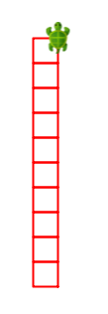
\includegraphics[scale=0.6]{../img/kojo/square-column}

  \columnbreak

  \begin{Code}
  def kvadrat = for (???) {???}
  for (???) {???}
  \end{Code}

  \end{multicols}
  \caption{En kvadratstapel.\label{fig:kojo-lab:column}}
\end{figure}

\Subtask %Kör ditt program med den \emph{gula} play-knappen. 
Studera hur anrop av proceduren \code{kvadrat} påverkar exekveringssekvensen av dina satser genom att göra lämpliga utskrifter så att du kan se när olika delar av koden exekveras. Vid vilka punkter i programmet sker ett ''hopp'' i sekvensen i stället för att efterföljande sats exekveras?  Använd lämpligt argument till \code{sakta} för att du ska hinna studera exekveringen.


\Subtask Rita samma bild med 10 staplade kvadrater (se bild \ref{fig:kojo-lab:column} på sidan \pageref{fig:kojo-lab:column}), men nu \emph{utan} att använda abstraktionen \code{kvadrat} -- använd i stället en nästlad repetition (alltså en upprepning inuti en upprepning). Vilket av de två sätten (med och utan abstraktionen \code{kvadrat}) är lättast att läsa? %\emph{Tips:} Varje gång du trycker på någon av play-knapparna, sparas ditt program. Du kan se dina sparade program om du klickar på \emph{Historik}-fliken. Du kan också stega bakåt och framåt i historiken med de blå pilarna bredvid play-knapparna.

\Subtask Generalisera din abstraktion \code{kvadrat} genom att ge den en parameter \code{sida: Double} som anger hur stor kvadraten blir. Rita flera kvadrater i likhet med bild \ref{fig:kojo-lab:resize} på sidan \pageref{fig:kojo-lab:resize}).

\begin{figure}[H]
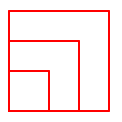
\includegraphics{../img/kojo/square-param}
  \caption{Olika stora kvadrater.\label{fig:kojo-lab:resize}}

\end{figure}



%\Subtask\Pen%\Checkpoint
%Se över ditt program i föregående uppgift och säkerställ att det är lättläst och följer en struktur som börjar med alla definitioner i logisk ordning och därefter fortsätter med huvudprogrammet.
%%Diskutera ditt program med en handledare.



%\Subtask\Pen Spara ditt program i en fil men lämpligt namn och ha programmet redo när det är din tur att redovisa vad du gjort under laborationen.
%Anteckna några åtgärder du vidtagit för att göra programmet mer lättläst.







\Task \emph{Alternativ.} \label{kojo:alt}

\Subtask Kör programmet nedan. Förklara vad som händer. %Använd den gula play-knappen för att studera exekveringen.

\begin{Code}
sakta(5000)

def move(key: Int): Unit = {
  println("key: " + key)
  if (key == 87) fram(10)
  else if (key == 83) fram(-10)
}

move(87); move('W'); move('W')
move(83); move('S'); move('S'); move('S')
\end{Code}

\Subtask \label{subtask:keypress}  Kör programmet nedan. Notera \code{activateCanvas} för att du ska slippa klicka i ritfönstret innan du kan styra paddan. Anropet \code{onKeyPress(move)} gör så att \code{move} kommer att anropas då en tangent trycks ned. Lägg till kod i \code{move} som gör att tangenten A ger en vridning moturs med 5 grader medan tangenten D ger en vridning medurs 5 grader. Med \code{onKeyPress} bestämmer man vilken procedur som ska köras vid tangenttryck.

\begin{Code}
sakta(0); activateCanvas

def move(key: Int): Unit = {
  println("key: " + key)
  if (key == 'W') fram(10)
  else if (key == 'S') fram(-10)
}

onKeyPress(move)
\end{Code}



%\Subtask Spara ditt program i en fil men lämpligt namn och ha programmet redo när det är din tur att redovisa vad du gjort under laborationen.


\subsection{Kontrollfrågor}\Checkpoint

\noindent Repetera teorin för denna vecka och var beredd på att kunna svara på dessa frågor när det blir din tur att redovisa vad du gjort under laborationen:

\begin{enumerate}
\item Vad innebär sekventiell exekvering av satser?
\item Vad är skillnaden mellan en sats och ett uttryck?
\item Vad är skillnaden mellan en procedur och en funktion?
\item Spelar ordningen mellan argument någon roll vid anrop av en funktion med flera parametrar?
\item Vad är en variabel? Ge exempel på deklaration, initialisering och tilldelning av variabler, samt användning av variabler i uttryck.
\item Vad är ett logiskt uttryck? Ge exempel på användning av logiska uttryck.
\item Vad är abstraktion? Ge exempel på användning av abstraktion.
\item Vad är nyttan med abstraktion?
\item Vad innebär sidoeffekt? Förklara och ge exempel.
\item Hur deklareras och initialiseras en variabel vars värde är förändringsbart?
\item Hur deklareras och initialiseras en variabel vars värde är oföränderligt?
\item Är det ett körtidsfel eller kompileringsfel att tilldela en oföränderlig variabel ett nytt värde?
\item Ange vilken av \code{for} och \code{while} som är lämpligast i dessa fall:
\begin{itemize}[noitemsep, nolistsep]
\item[A.] Summera de hundra första heltalen.
\item[B.] Räkna antal tecken i en sträng innan första blanktecken.
\item[C.] Dra 100 slumptal mellan 1 och 6 och summera de tal som är mindre än 3.
\item[D.] Summera de första heltalen från 1 och uppåt tills summan är minst 100.
\end{itemize}
\end{enumerate}


\subsection{Frivilliga extrauppgifter}

\noindent Gör i mån intresse och träningsbehov nedan uppgifter i valfri ordning.

\Task \emph{Abstraktion och generalisering}.

\Subtask Skapa en abstraktion \code{def stapel = ???} som använder din abstraktion \code{kvadrat}.

\Subtask Du ska nu \emph{generalisera} din procedur så att den inte bara kan rita exakt 10 kvadrater i en stapel. Ge proceduren \code{stapel} en parameter \code{n} som styr hur många kvadrater som ritas.
\begin{Code}
def kvadrat = ???
def stapel(n: Int) = ???

sakta(100)
stapel(42)
\end{Code}



\Subtask Rita nedan bild med hjälp av abstraktionen \code{stapel}. Det är totalt 100 kvadrater och varje kvadrat har sidan 25. \emph{Tips:} Med ett negativt argument till procedur \code{hoppa} kan du få sköldpaddan att hoppa baklänges utan att rita, t.ex. \code{hoppa(-10*25)}

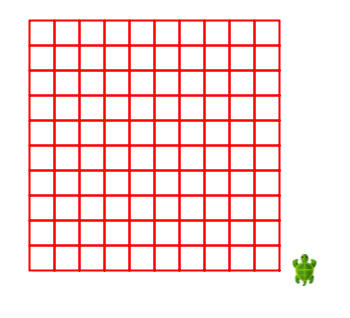
\includegraphics[width=0.3\textwidth]{../img/kojo/square-grid}

\Subtask Generalisera dina abstraktioner \code{kvadrat} och \code{stapel} så att man kan påverka storleken på kvadraterna som ritas ut.

\Subtask Skapa en abstraktion \code{rutnät} med lämpliga parametrar som gör att man kan rita rutnät med olika stora kvadrater och olika många kvadrater i både x- och y-led.

\Subtask Generalisera dina abstraktioner \code{kvadrat} och \code{stapel} så att man kan påverka fyllfärgen och pennfärgen för kvadraterna som ritas ut.

\Task \emph{Växling med booleska värden.}

\Subtask Bygg vidare på programmet i uppgift \ref{kojo:alt} och lägg till nedan kod i början av programmet. Lägg även till kod som gör så att om man trycker på tangenten G så sätts rutnätet omväxlande på och av. Observera att det är exakt \emph{en} procedur som anropas vid \code{onKeyPress}.

\begin{Code}
var isGridOn = false

def toggleGrid =
  if (isGridOn) {
    gridOff
    isGridOn = false
  } else {
    gridOn
    isGridOn = true
  }
\end{Code}

\Subtask Gör så att när man trycker på tangenten X så sätter man omväxlande på och av koordinataxlarna. Använd en variabel \code{isAxesOn} och definiera en abstraktion \code{toggleAxes} som anropar \code{axesOn} och \code{axesOff} på liknande sätt som i föregående uppgift.


\Task \emph{Repetition.}~Skriv en procedur \code{randomWalk} med detta huvud: \\
\code{def randomWalk(n: Int, maxStep: Int, maxAngle: Int): Unit}\\ som gör så att paddan tar \code{n} steg av slumpmässig längd mellan \code{0} och \code{maxStep}, samt efter varje steg vrider sig åt vänster en slumpmässig vinkel mellan \code{0} och \code{maxAngle}. Anropa din procedur med olika argument och undersök hur dess värden påverkar bildens utseende. \emph{Tips:} Uttrycket \code{math.random() * 100} ger ett tal från 0 till (nästan) 100. Du kan styra hur långsamt paddan ritar genom anrop av \code{sakta(???)} (prova dig fram till något  lämpligt heltalsargument i stället för \code{???}).
\vspace{2em}\\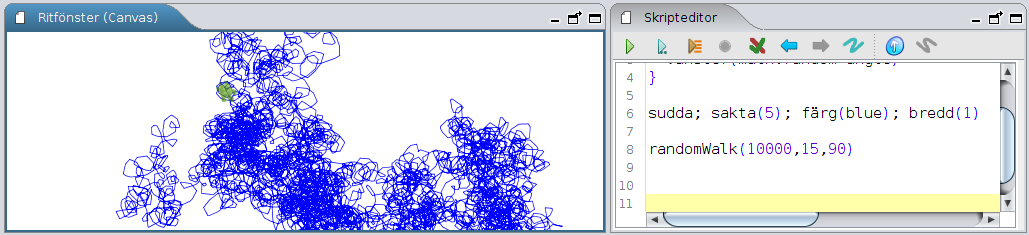
\includegraphics[width=\textwidth]{../img/kojo/random-walk.png}


\Task \emph{Variabler, namngivning och formatering.}

\Subtask Klistra in nedan konstigt formatterade program \emph{exakt} som det står med blanktecken, indragningar och radbrytningar. Kör programmet och förklara vad som händer.

\begin{figure}[H]
\begin{Code}
// Ett konstigt formaterat program med en del konstiga namn.

def gurka(x: Double,
y: Double, namn: String,
typ: String,
värde:String) = {
val tomat = 15
val h = 30
hoppaTill(x,y)
norr
skriv(namn+": "+typ)
hoppaTill(x+tomat*(namn.size+typ.size),y)
skriv(värde); söder; fram(h); vänster
fram(tomat * värde.size); vänster
fram(h); vänster
fram(tomat * värde.size); vänster }
sudda; färg(svart); val s = 130
val h = 40
var x = 42; gurka(10, s-h*0, "x","Int", x.toString)
var y = x; gurka(10, s-h*1, "y","Int", y.toString)
x = x + 1; gurka(10, s-h*2, "x","Int", x.toString)
gurka(10, s-h*3, "y","Int", y.toString); osynlig
\end{Code}
\end{figure}

\Subtask\Pen Skriv ner namnet på alla variabler som förekommer i programmet.

\Subtask\Pen Vilka av dessa variabler är lokala?

\Subtask\Pen Vilka av dessa variabler kan förändras efter initialisering?

\Subtask\Pen Föreslå tre förändringar av programmet ovan (till exempel namnbyten) som gör att det blir lättare att läsa och förstå.

\Subtask Gör sök-ersätt av \code{gurka} till ett bättre namn. \emph{Tips:} undersök kontextmenyn i editorn i Kojo genom att högerklicka. Använd kortkommandot för Sök/Ersätt.

\Subtask Gör automatisk formatering av koden med hjälp av lämpligt kortkommando. Notera skillnaderna. Vilka autoformateringar gör programmet lättare att läsa? Vilka manuella formateringar tycker du bör göras för att öka läsbarheten? Ge funktionen \code{gurka} ett bättre namn.  Diskutera läsbarheten med en handledare.



\Task \label{task:measuretime} \emph{Tidmätning.} Hur snabb är din dator?

\Subtask \label{task:timer} Skriv in koden nedan i Kojos editor och kör upprepade gånger med den gröna play-knappen. Tar det lika lång tid varje gång? Varför?

\begin{Code}
object timer {
  def now: Long = System.currentTimeMillis
  var saved: Long = now
  def elapsedMillis: Long = now - saved
  def elapsedSeconds: Double = elapsedMillis / 1000.0
  def reset: Unit = { saved = now }
}

// HUVUDPROGRAM:
timer.reset
var i = 0L
while (i < 1e8.toLong) { i += 1 }
val t = timer.elapsedSeconds
println("Räknade till " + i + " på " + t + " sekunder.")
\end{Code}


\Subtask Ändra i loopen i uppgift \ref{task:timer}) så att den räknar till 4.4 miljarder. Hur lång tid tar det för din dator att räkna så långt?\footnote{Det går att göra ungefär en heltalsaddition per klockcykel per kärna. Den första elektroniska datorn \href{https://sv.wikipedia.org/wiki/ENIAC}{Eniac} hade en klockfrekvens motsvarande 5 kHz. Den dator på vilken denna övningsuppgift skapades hade en i7-4790K turboklockad upp till 4.4 GHz.
%\href{http://www.extremetech.com/computing/185512-overclocking-intels-core-i7-4790k-can-devils-canyon-fix-haswells-low-clock-speeds/2}{www.extremetech.com/computing/185512-overclocking-intels-core-i7-4790k-can-devils-canyon-fix-haswells-low-clock-speeds/2}
}

\Subtask  Om du kör på en Linux-maskin: Kör nedan Linux-kommando upprepade gånger i ett terminalfönster. Med hur många MHz kör din dators klocka för tillfället? Hur förhåller sig klockfrekvensen till antalet rundor i while-loopen i föregående uppgift? (Det kan hända att din dator kan variera centralprocessorns klockfrekvens. Prova både medan du kör tidmätningen i Kojo och då din dator ''vilar''. Vad är det för poäng med att en processor kan variera sin klockfrekvens?)
\begin{REPLnonum}
> lscpu | grep MHz
\end{REPLnonum}


\Subtask Ändra i koden i uppgift \ref{task:timer}) så att \code{while}-loopen bara kör 5 gånger. %Kör programmet med den \emph{gula} play-knappen. Scrolla i programspårningen och förklara vad som händer. Klicka på \code{CALL}-rutorna och se vilken rad som markeras i ditt program.

\Subtask Lägg till koden nedan i ditt program och försök ta reda på ungefär hur långt din dator hinner räkna till på en sekund för \code{Long}- respektive \code{Int}-variabler. Använd den gröna play-knappen.
\begin{CodeSmall}
def timeLong(n: Long): Double = {
  timer.reset
  var i = 0L
  while (i < n) { i += 1 }
  timer.elapsedSeconds
}

def timeInt(n: Int): Double = {
  timer.reset
  var i = 0
  while (i < n) { i += 1 }
  timer.elapsedSeconds
}

def show(msg: String, sec: Double): Unit = {
  print(msg + ": ")
  println(sec + " seconds")
}

def report(n: Long): Unit = {
  show("Long " + n, timeLong(n))
  if (n <= Int.MaxValue) show("Int  " + n, timeInt(n.toInt))
}

// HUVUDPROGRAM, mätningar:

report(Int.MaxValue)
for (i <- 1 to 10) report(4.26e9.toLong)
\end{CodeSmall}

\Subtask Hur mycket snabbare går det att räkna med \code{Int}-variabler jämfört med \code{Long}-variabler? Diskutera gärna svaret med en handledare.

\Task Lek med färg i Kojo. Sök på internet efter dokumentationen för klassen \code{java.awt.Color} och studera vilka heltalsparametrar den sista konstruktorn i listan med konstruktorer tar för att skapa sRGB-färger. Om du högerklickar i editorn i Kojo och väljer ''Välj färg...'' får du fram färgväljaren och med den kan du välja fördefinierade färger eller blanda egna färger. När du har valt färg får du se vilka parametrar till \code{java.awt.Color} som skapar färgen. Testa detta i REPL:

\begin{REPL}
scala> val c = new java.awt.Color(124,10,78,100)
c: java.awt.Color = java.awt.Color[r=124,g=10,b=78]

scala> c.  // tryck på TAB
asInstanceOf    getColorComponents      getRGBComponents
brighter        getColorSpace           getRed
createContext   getComponents           getTransparency
darker          getGreen                isInstanceOf
getAlpha        getRGB                  toString
getBlue         getRGBColorComponents

scala> c.getAlpha
res3: Int = 100
\end{REPL}
Skriv ett program som ritar många figurer med olika färger, till exempel cirklar som nedan. Om du använder alfakanalen blir färgerna genomskinliga.

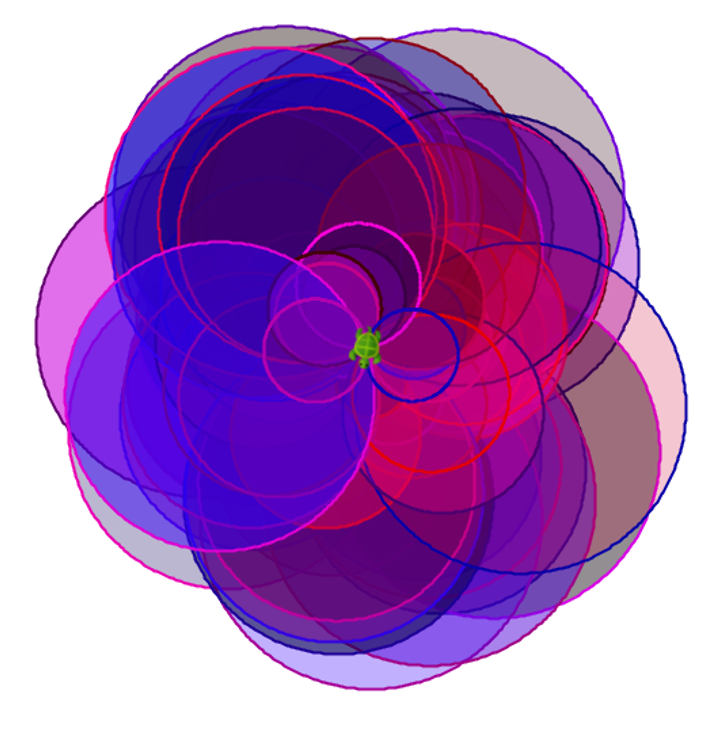
\includegraphics[width=0.82\textwidth]{../img/kojo/random-color-circles.png}


\Task Ladda ner ''Uppdrag med Kojo'' från \href{http://lth.se/programmera/uppdrag}{lth.se/programmera/uppdrag}  och gör några uppgifter som du tycker verkar intressanta.

%\Subtask ''Programming Fundamentals with Kojo'' som kan laddas ner här:\\
%\href{http://wiki.kogics.net/kojo-codeactive-books}{wiki.kogics.net/kojo-codeactive-books}

\Task Om du vill jobba med att hjälpa skolbarn att lära sig programmera med Kojo, kontakta \url{http://www.vattenhallen.lth.se} och anmäl ditt intresse att vara handledare.


%!TEX encoding = UTF-8 Unicode
%!TEX root = ../compendium1.tex

\renewcommand{\vecka}{2}

\chapter{Kodstrukturer}\label{chapter:W02}
\begin{itemize}[nosep]
\item samling: Range
\item for-uttryck
\item map
\item foreach
\item flatMap
\item algoritm vs implementation
\item pseudokod
\item algoritm: swap
\item algoritm: summering
\item algoritm: min/max
\item paket
\item import
\item filstruktur
\item jar
\item dokumentation
\item programlayout
\item JDK
\item konstanter vs föränderlighet
\item objektorientering
\item klasser
\item objekt
\item punktnotation
\item referensvariabler
\item referenstilldelning
\item anropa metoder
\item block
\item namnsynlighet
\item namnöverskuggning
\item SimpleWindow
\end{itemize}

%!TEX encoding = UTF-8 Unicode
%!TEX root = ../lect-week02.tex

%\Subsection{Samlingar och loopar}
\Subsection{Datastrukturer och kontrollstrukturer}


\begin{Slide}{Vad är en datastruktur?}\SlideFontSmall
\begin{itemize}
\item En \href{https://sv.wikipedia.org/wiki/Datastruktur}{datastruktur} är en struktur för organisering av data som...
\begin{itemize}\SlideFontTiny
\item kan innehålla \Alert{många} element,
\item kan refereras till med \Alert{ett} enda namn, och
\item ger möjlighet att komma åt de enskilda elementen.
\end{itemize}

\item En \Emph{samling} \Eng{collection} är en datastruktur som kan innehålla många element av \Alert{samma typ}.

\item Exempel på olika samlingar där elementen är organiserade på olika vis: \\ 
\vspace{0.5em}
\begin{tabular}{l c}
\Emph{Lista} & 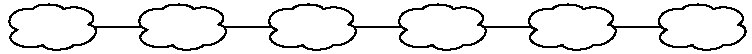
\includegraphics[width=5cm]{../img/list.pdf} \\
\Emph{Träd}  & 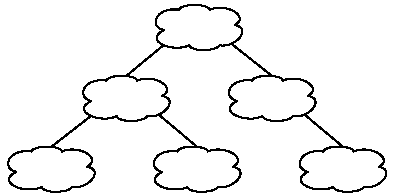
\includegraphics[width=2.2cm]{../img/tree.pdf} \\
\Emph{Graf}  & 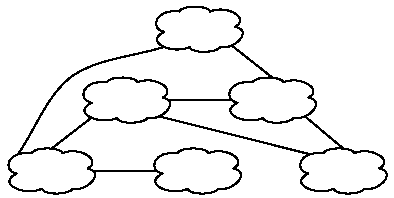
\includegraphics[width=2.2cm]{../img/graph.pdf} \\
\end{tabular}
\end{itemize}
{
\SlideFontTiny \vspace{1em }\hskip2em
Mer om listor \& träd \href{http://cs.lth.se/edaa01vt}{fördjupningskursen}. 
Mer om träd, grafer i \href{http://cs.lth.se/edaa40}{Diskreta strukturer.}
}

\end{Slide} 


\begin{Slide}{Vad är en vektor?}\SlideFontSmall
En \Emph{vektor}\footnote{Vektor kallas ibland på svenska även \href{https://sv.wikipedia.org/wiki/F\%C3\%A4lt_\%28datastruktur\%29}{fält}, men det skapar stor förvirring eftersom det engelska ordet \emph{field} ofta används för \emph{attribut} (förklaras senare).} 
\Eng{vector, \href{https://en.wikipedia.org/wiki/Array_data_structure}{array}} är en \Emph{samling} som är \Alert{snabb} att \Emph{indexera} i. 
Åtkomst av element sker med \code{apply(platsnummer)}: 

\begin{REPL}
scala> val heltal = Vector(42, 13, -1, 0 , 1)
heltal: scala.collection.immutable.Vector[Int] = Vector(42, 13, -1, 0, 1)

scala> heltal.apply(0)
res0: Int = 42

scala> heltal(1)    // man kan skippa .apply
res1: Int = 13

scala> heltal(5)
java.lang.IndexOutOfBoundsException: 5
  at scala.collection.immutable.Vector.checkRangeConvert(Vector.scala:132)
\end{REPL}
Utelämnar du \code{.apply} så gör kompilatorn anrop av \code{apply} ändå om det går.
\end{Slide}

\begin{Slide}{En konceptuell bild av en vektor}

\begin{REPLnonum}
scala> val heltal = Vector(42, 13, -1, 0 , 1)

scala> heltal(0)
res0: Int = 42
\end{REPLnonum}

\begin{tikzpicture}[font=\ttfamily]
\matrix [matrix of nodes, row sep=0, column 2/.style={nodes={rectangle,draw,minimum width=3em}}] (var) at (0cm, 2.8cm)
{
heltal   &  \makebox(16,12){ }\\
};
\matrix [matrix of nodes, draw=black,row sep=0, column 2/.style={nodes={rectangle,draw,minimum width=4em}}] (vec) at (4cm, 1cm)
{
\textit{plats} &  \\
0   &  \makebox(16,12){42}\\
1   &  \makebox(16,12){13}\\
2   &  \makebox(16,12){-1}\\
3   &  \makebox(16,12){0}\\
4   &  \makebox(16,12){1}\\
};
\filldraw[black] (0.7cm,2.8cm) circle (3pt) node[] (ref) {};
 \draw [arrow] (ref) -- (vec);
\end{tikzpicture}

%\vspace{1em} Elementen ligger på rad någonstans i minnet.
\end{Slide}



\begin{Slide}{En samling strängar}

\begin{itemize}
\item En vektor kan lagra många värden av samma typ. 
\item Elementen kan vara till exempel heltal eller strängar. 
\item Eller faktiskt vad som helst. 
\end{itemize}

\begin{REPL}
scala> val grönsaker = Vector("gurka","tomat","paprika","selleri")
grönsaker: scala.collection.immutable.Vector[String] = Vector(gurka, tomat, paprika, selleri)

scala> val g = grönsaker(1)
g: String = tomat

scala> val xs = Vector(42, "gurka", true, 42.0)
xs: scala.collection.immutable.Vector[Any] = Vector(42, gurka, true, 42.0)


\end{REPL}

\end{Slide}

\begin{Slide}{Vad är en kontrollstruktur?}
\begin{itemize}
\item En \Emph{kontrollstruktur} påverkar \Alert{sekvensen}.
\begin{itemize}
\item[] Exempel på inbyggda kontrollstrukturer: 
\\\vspace{0.5em}\code{for}-sats, \code{while}-sats
\end{itemize}

\item[]

\item I Scala kan man definiera \Emph{egna} kontrollstrukturer.
\begin{itemize}
\item[] Exempel: \code{upprepa} som du använt i Kojo
\\\vspace{0.5em}\code|upprepa(4){fram; höger}|
\end{itemize}
\end{itemize}
\end{Slide}


\begin{Slide}{Mitt första program: en oändlig loop på ABC80}
\begin{columns}
\begin{column}{0.8\textwidth}
\begin{verbatim}
10 print "hej"
20 goto 10
\end{verbatim}
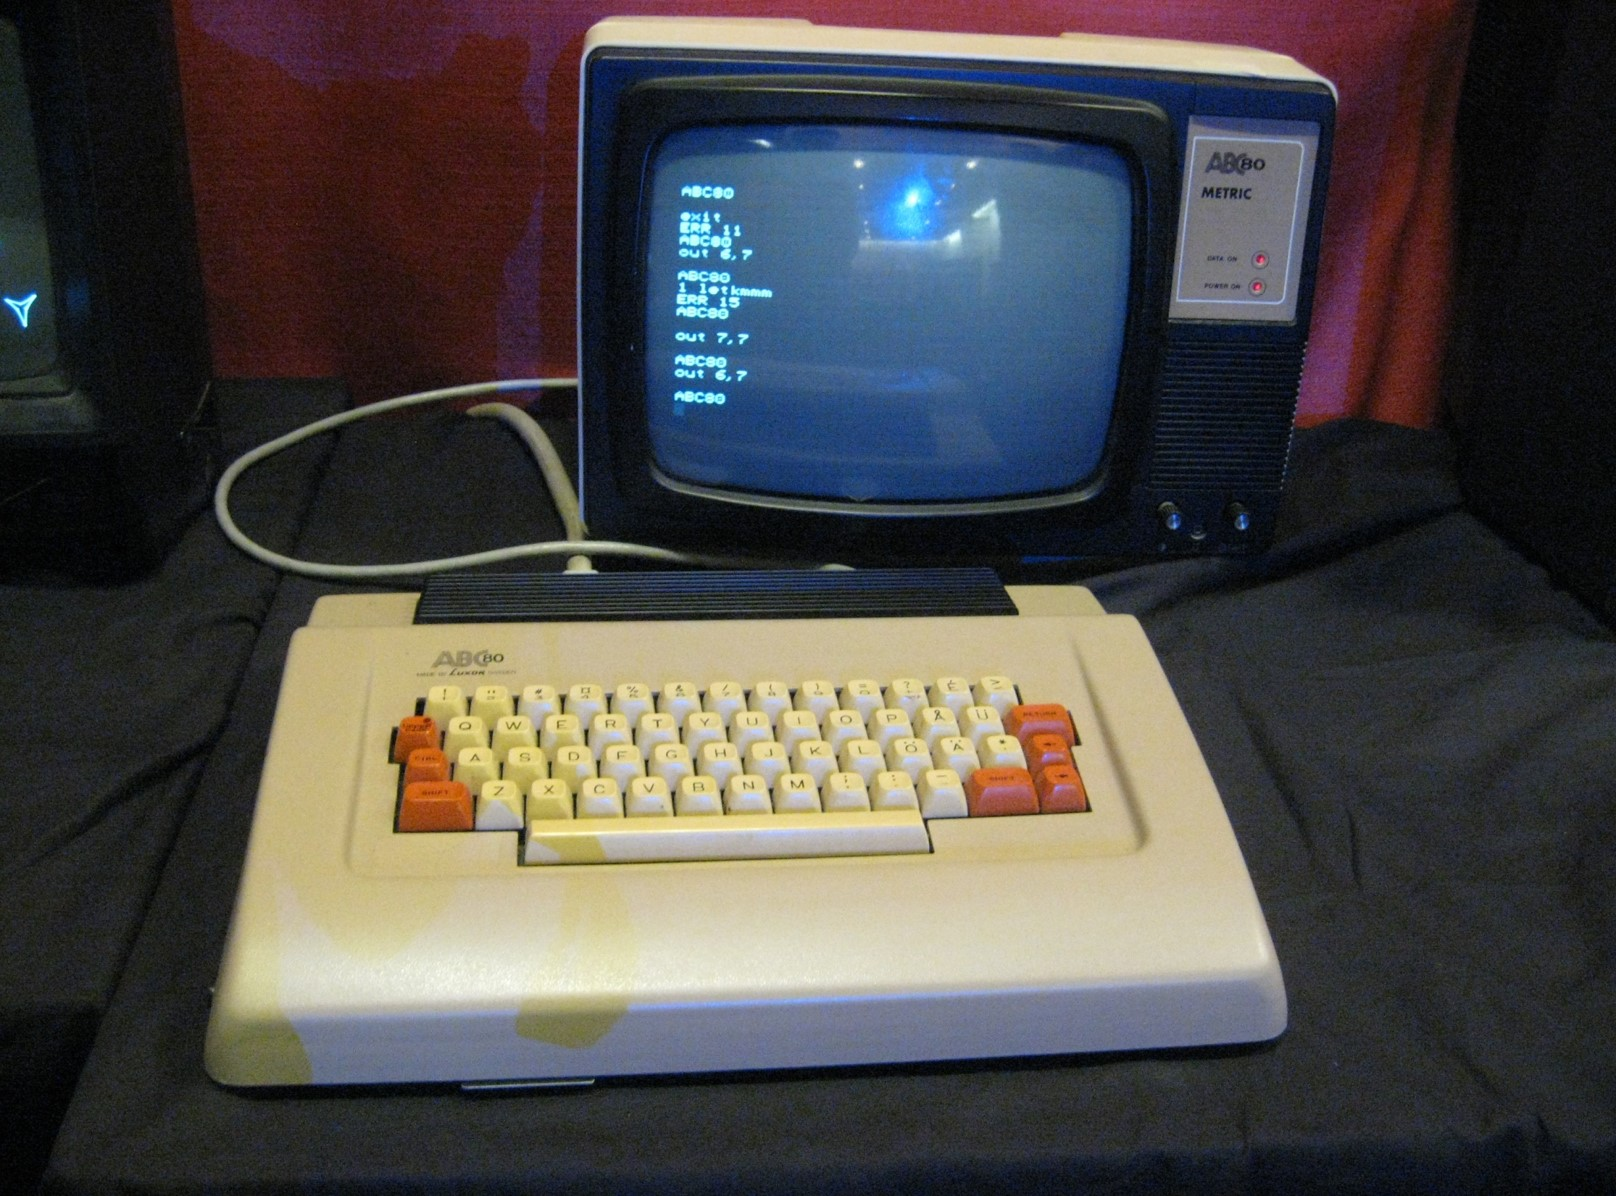
\includegraphics[width=0.8\textwidth]{../img/abc80.jpg}
\end{column}
\begin{column}{0.3\textwidth}
\pause
\begin{verbatim}
hej
hej
hej
hej
hej
hej
hej
hej
hej
hej
hej
hej
<Ctrl+C>
\end{verbatim}

\end{column}
\end{columns}
\end{Slide}


\begin{Slide}{Loopa genom elementen i en vektor}
En \code{for}-\Emph{sats} som skriver ut alla element i en vektor:
\begin{REPL}
scala> val grönsaker = Vector("gurka","tomat","paprika","selleri")

scala> for (g <- grönsaker) println(g)
gurka
tomat
paprika
selleri

\end{REPL}

\end{Slide}


\begin{Slide}{Bygga en ny samling från en befintlig med for-uttryck}
Ett \code{for}-\code{yield}-\Emph{uttryck} som \Emph{skapar en \Alert{ny} samling}.

\begin{Code}[basicstyle=\ttfamily\fontsize{12}{14}\selectfont]
for (g <- grönsaker) yield "god " + g
\end{Code}

\begin{REPL}
scala> val grönsaker = Vector("gurka","tomat","paprika","selleri")

scala> for (g <- grönsaker) yield "god " + g
res0: scala.collection.immutable.Vector[String] = 
  Vector(god gurka, god tomat, god paprika, god selleri)

scala> val åsikter = for (g <- grönsaker) yield s"god $g"
åsikter: scala.collection.immutable.Vector[String] = 
  Vector(god gurka, god tomat, god paprika, god selleri)
\end{REPL}

\end{Slide}


\begin{Slide}{Samlingen \code{Range} håller reda på intervall}
\begin{itemize}
\item Med en \code{Range(start, slut)} kan du skapa ett intervall: \\ från och med \code{start} till (men inte med) \code{slut}
\end{itemize}

\begin{REPLnonum}
scala> Range(0, 42)
res0: scala.collection.immutable.Range = 
  Range(0, 1, 2, 3, 4, 5, 6, 7, 8, 9, 10, 11, 12, 13, 14, 
    15, 16, 17, 18, 19, 20, 21, 22, 23, 24, 25, 26, 27, 28, 
    29, 30, 31, 32, 33, 34, 35, 36, 37, 38, 39, 40, 41)
\end{REPLnonum}

\begin{itemize}
\item Men alla värden däremellan skapas inte förrän de behövs:
\end{itemize}

\begin{REPL}
scala> val jättestortIntervall = Range(0, Int.MaxValue)
jättestortIntervall: scala.collection.immutable.Range = Range(0, 1, 2, 3, 4, 5, ...

scala> jättestortIntervall.end
res1: Int = 2147483647

scala> jättestortIntervall.toVector
java.lang.OutOfMemoryError: GC overhead limit exceeded
\end{REPL}

\end{Slide}

\begin{Slide}{Loopa med Range}
\code{Range} används i for-lopar för att hålla reda på antalet rundor.
\begin{REPLnonum}
scala> for (i <- Range(0, 6)) print(" gurka " + i)
 gurka 0 gurka 1 gurka 2 gurka 3 gurka 4 gurka 5 
\end{REPLnonum}
Du kan skapa en \code{Range} med \code{until} efter ett heltal:
\begin{REPLnonum}
scala> 1 until 7
res1: scala.collection.immutable.Range = 
  Range(1, 2, 3, 4, 5, 6)

scala> for (i <- 1 until 7) print(" tomat " + i) 
 tomat 1 tomat 2 tomat 3 tomat 4 tomat 5 tomat 6

\end{REPLnonum}
\end{Slide}

\begin{Slide}{Loopa med Range skapad med \texttt{to}}

Med \code{to} efter ett heltal får du en \code{Range} till och \Emph{med} sista:
\begin{REPLnonum}
scala> 1 to 6
res2: scala.collection.immutable.Range.Inclusive = 
  Range(1, 2, 3, 4, 5, 6)

scala> for (i <- 1 to 6) print(" gurka " + i) 
 gurka 1 gurka 2 gurka 3 gurka 4 gurka 5 gurka 6
 
\end{REPLnonum}


\end{Slide}



\begin{Slide}{Vad är en \code{Array} i JVM?}


\begin{itemize}
\item En \code{Array} liknar en \code{Vector} men har en särställning i JVM:
\begin{itemize}
\item Lagras som en sekvens i minnet på efterföljande adresser.
\item \Emph{Fördel}: snabbaste samlingen för element-access i JVM.
\item Men det finns en hel del \Alert{nackdelar} som vi ska se senare.
\end{itemize}

\end{itemize}

\begin{REPLnonum}
scala> val heltal = Array(42, 13, -1, 0 , 1)
\end{REPLnonum}

\begin{tikzpicture}[font=\ttfamily,scale=0.75, every node/.style={scale=0.75}]
\matrix [matrix of nodes, row sep=0, column 2/.style={nodes={rectangle,draw,minimum width=3em}}] (var) at (0cm, 2.8cm)
{
heltal   &  \makebox(16,12){ }\\
};
\matrix [matrix of nodes, draw=black,row sep=0, column 2/.style={nodes={rectangle,draw,minimum width=4em}}] (vec) at (4cm, 1cm)
{
\textit{plats} &  \\
0   &  \makebox(16,12){42}\\
1   &  \makebox(16,12){13}\\
2   &  \makebox(16,12){-1}\\
3   &  \makebox(16,12){0}\\
4   &  \makebox(16,12){1}\\
};
\filldraw[black] (0.7cm,2.8cm) circle (3pt) node[] (ref) {};
 \draw [arrow] (ref) -- (vec);
\end{tikzpicture}
\end{Slide}

\begin{Slide}{Några likheter \& skillnader mellan \texttt{Vector} och \texttt{Array}}\SlideFontSmall
\begin{multicols}{2}
\begin{REPL}[numbers=none]
scala> val xs = Vector(1,2,3)
\end{REPL}

\columnbreak

\begin{REPL}[numbers=none]
scala> val xs = Array(1,2,3)
\end{REPL}
\end{multicols}


Några likheter mellan \texttt{Vector} och \texttt{Array}
\begin{itemize}
\item Båda är samlingar som kan innehålla många element.

\item Med båda kan man snabbt accessa vilket element som helst: \code{xs(2)}

\item Båda har en fix storlek efter allokering.
\end{itemize}

Några viktiga skillnader:
\begin{multicols}{2}
\Emph{Vector}
\begin{itemize}
\item Är \Emph{oföränderlig}: du kan lita på att elementreferenserna aldrig någonsin kommer att ändras.

\item Är \Emph{snabb på att skapa en delvis förändrad kopia}, t.ex. tillägg/borttagning/uppdatering mitt i sekvensen.

\end{itemize}


\columnbreak

\Alert{Array}
\begin{itemize}
\item Är \Alert{föränderlig}: \code{xs(2) = 42}

\item Är \Alert{snabb} om man bara vill läsa eller skriva på befintliga platser.

\item Är \Alert{långsam} om man vill lägga till eller ta bort element mitt i sekvensen.

\end{itemize}
\end{multicols}
\end{Slide}



\Subsection{Huvudprogram med \texttt{main} i Scala och Java}

\begin{Slide}{Ett minimalt fristående program i Scala och Java}
Nedan Scala-kod skrivs i en editor, spara med valfritt filnamn:
\begin{Code}
// this is Scala 

object Hello {
  def main(args: Array[String]): Unit = {
    println("Hejsan scala-appen!")
  }
}
\end{Code}

\pause
\vspace{1em}
Nedan Java-kod skrivs i en editor, filen \Alert{måste} heta \texttt{Hi.java}

\begin{Code}[language=Java]
// this is Java 

public class Hi {
    public static void main(String[] args) {
        System.out.println("Hejsan Java-appen!");
    }
}
\end{Code}

\end{Slide}


\begin{Slide}{Loopa genom en samling med en \texttt{while}-sats}
\begin{REPLnonum}
scala> val xs = Vector("Hej","på","dej","!!!")
xs: scala.collection.immutable.Vector[String] = 
  Vector(Hej, på, dej, !!!)

scala> xs.size
res0: Int = 4

scala> var i = 0
i: Int = 0

scala> while (i < xs.size) { println(xs(i)); i = i + 1 }
Hej
på
dej
!!!
\end{REPLnonum}
\end{Slide}


\begin{Slide}{Loopa genom argumenten i ett Scala-huvudprogram}
Skriv denna kod och spara i filen \texttt{helloargs.scala}
\begin{REPL}[numbers=none]
$ gedit helloargs.scala
\end{REPL}
\begin{Code}
object HelloScalaArgs {
  def main(args: Array[String]): Unit = {
    var i = 0
    while (i < args.size) { 
      println(args(i))
      i = i + 1
    }
  }
}
\end{Code}
Kompilera och kör:
\begin{REPL}
$ scalac helloargs.scala
$ scala HelloScalaArgs hej gurka tomat 
hej
gurka
tomat
\end{REPL}
\end{Slide}


\begin{Slide}{Loopa genom argumenten i ett Java-huvudprogram}
\begin{REPL}[numbers=none]
$ gedit HelloJavaArgs.java
\end{REPL}
\begin{Code}[language=Java]
// this is Java 

public class HelloJavaArgs {
    public static void main(String[] args) {
    int i = 0;
    while (i < args.length) { 
      System.out.println(args[i]);
      i = i + 1;
    }
  }
}
\end{Code}
Kompilera och kör:
\begin{REPL}
$ javac HelloJavaArgs.scala
$ java HelloJavaArgs hej gurka tomat 
hej
gurka
tomat
\end{REPL}

\end{Slide}


\begin{Slide}{Scala-skript}
\begin{itemize}
\item Skala-kod kan köras som ett \Emph{skript}.\footnote{\SlideFontTiny Du får prova detta på övningen. Vi kommer mest att köra kompilerat i kursen, då Scala-skript saknar mekanism för inkludering av andra skript. Men det finns ett öppenkällkodsprojekt som löser det: \url{http://www.lihaoyi.com/Ammonite/}
}
\item Ett skript kompileras varje gång innan det körs och maskinkoden sparas inte som vid vanlig kompilering.
\item Då behövs ingen \code{main} och inget \code{object}
\end{itemize}

\begin{Code}[basicstyle=\ttfamily\fontsize{10}{12}\selectfont]
// spara nedan i filen 'myscript.scala'

println("Hejsan argumnet!")
for (arg <- args) println(arg)
\end{Code}

\begin{REPLnonum}
$ scala myscript.scala
\end{REPLnonum}


\end{Slide}



\Subsection{Algoritmer: stegvisa lösningar}

\begin{Slide}{Vad är en algoritm?}
En \href{https://sv.wikipedia.org/wiki/Algoritm}{algoritm} är en sekvens av instruktioner som beskriver \\hur man löser ett problem.\\
\vspace{1em}
\Emph{Exempel}: 
\begin{itemize}
\item	 baka en kaka 
\pause\item räkna ut din pensionsprognos 
\pause\item köra bil 
\pause\item kolla om highscore i ett spel 
\item ...
\end{itemize}

\begin{tikzpicture}[overlay]
\node[xshift=0.85\textwidth, scale=2.0] at (0,1.3) { 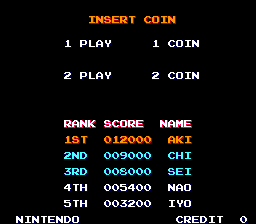
\includegraphics[width=0.25\textwidth]{../img/highscore}};
\end{tikzpicture}
\end{Slide}



\begin{Slide}{Algoritm-exempel: HIGHSCORE}
\Emph{Problem}: Kolla om high-score i ett spel \\ \vspace{1em}

\Emph{Varför?} \pause Så att de som spelar uppmuntras att spela mer :) \\ \vspace{1em}

\Emph{Algoritm:}\pause
\begin{enumerate}
\item $points$ $\leftarrow$ poängen efter senaste spelet
\item $highscore$ $\leftarrow$ bästa resultatet innan senaste spelet
\item \Key{om} $points$ är större än $highscore$ 
\begin{enumerate}[ ~~]
\item  Skriv ''Försök igen!''
\end{enumerate}
\Key{annars}
\begin{enumerate}[ ~~]
\item  Skriv ''Grattis!''
\end{enumerate}
\end{enumerate}
\pause
\scriptsize \Alert{Hittar du buggen?}
\end{Slide}


\begin{Slide}{HIGHSCORE implementerad i Scala}
\begin{Code}
import scala.io.StdIn.readLine

object HighScore {
  def main(args: Array[String]): Unit = {
    val points = readLine("Hur mång poäng fick du?").toInt
    val highscore = readLine("Vad var highscore före senaste spelet?").toInt
    val msg = if (points > highscore) "GRATTIS!" else "Försök igen!"
    println(msg) 
  }
}
\end{Code}
\pause
Är det en bugg eller en feature att det står\\ \texttt{points > highscore} \\ och inte \\ \texttt{points >= highscore} \\ ?
% Buggen är att man inte får GRATTIS om poäng == highscore vilket är tråkigt :)
\end{Slide}


\begin{Slide}{HIGHSCORE implementerad i Java}
\begin{Code}[language=Java]
import java.util.Scanner;

public class HighScore {
    public static void main(String[] args){
        Scanner scan = new Scanner(System.in);
        System.out.println("Hur många poäng fick du?");
        int points =  scan.nextInt();
        System.out.println("Vad var higscore före senaste spelet?");
        int highscore = scan.nextInt();
        if (points > highscore) {
            System.out.println("GRATTIS!");
        } else {
            System.out.println("Försök igen!");
        }
    }
}
\end{Code}
\end{Slide}


\begin{Slide}{Algoritmexempel: N-FAKULTET}
\begin{algorithm}[H]
 \SetKwInOut{Input}{Indata}\SetKwInOut{Output}{Resultat}

 \Input{heltalet $n$}
 \Output{utskrift av produkten av de första $n$ heltalen }
 ~\\
 $prod \leftarrow 1$ \\
 $i \leftarrow 2$  \\
 \While{$i \leq n$}{
  $prod \leftarrow prod * i$\\
  $i \leftarrow i + 1$
 }
 skriv ut $prod$
\end{algorithm}
\pause\vspace{1em}
\begin{itemize}\SlideFontSmall
\item Vad händer om $n$ är noll?
\item Vad händer om $n$ är ett?
\item Vad händer om $n$ är två?
\item Vad händer om $n$ är tre?
\end{itemize}
\end{Slide}

\begin{Slide}{Algoritmexempel: MIN}
\begin{algorithm}[H]
 \SetKwInOut{Input}{Indata}\SetKwInOut{Output}{Resultat}

 \Input{Array $args$ med strängar som alla innehåller heltal}
 \Output{utskrift av minsta heltalet }
 ~\\
 $min \leftarrow$ det största heltalet som kan uppkomma  \\
 $n \leftarrow $ antalet heltal \\
 $i \leftarrow 0$ \\
 \While{$i < n$}{
   $x \leftarrow args(i).toInt$ \\
   \If{( x < $min$)}{$min \leftarrow x$}
   $i \leftarrow i + 1$
 }
 skriv ut $min$
\end{algorithm}
\pause{\hfill \SlideFontTiny \Emph{Test med indata}: \code{args = Array("2", "42", "1", "2")}}
\end{Slide}


\Subsection{Funktioner skapar struktur}

\begin{Slide}{Mall för funktionsdefinitioner}

\code{def} funktionsnamn(parameterdeklarationer): returtyp = block

\pause\vspace{0.5em}\Emph{Exempel}:

\begin{Code}[basicstyle=\ttfamily\fontsize{9}{11}\selectfont]
def öka(i: Int): Int = { i + 1 }
\end{Code}
\pause Om ett enda uttryck: behövs inga \code|{}|. Returtypen kan härledas.
\begin{Code}[basicstyle=\ttfamily\fontsize{9}{11}\selectfont]
def öka(i: Int) = i + 1  
\end{Code}
\pause Om flera parametrar, separera dem med kommatecken: 
\begin{Code}[basicstyle=\ttfamily\fontsize{9}{11}\selectfont]
def isHighscore(points: Int, high: Int): Boolean = {
  val highscore: Boolean = points > high
  if (highscore) println(":)") else print(":(")
  highscore
}
\end{Code}
\pause Ovan funktion har \Alert{sidoeffekten} att skriva ut en smiley.
\end{Slide}

\begin{Slide}{Bättre många små abstraktioner som gör en sak var}

\begin{Code}[basicstyle=\ttfamily\fontsize{8}{11}\selectfont]
def isHighscore(points: Int, high: Int): Boolean = points > high

def printSmiley(isHappy: Boolean): Unit = 
  if (isHappy) println(":)") else print(":(")
\end{Code}

\pause\vspace{2em}
\begin{REPLnonum}
  printSmiley(isHighscore(113,99))
\end{REPLnonum}

\pause\vspace{2em} \code{isHigscore} är en \Emph{äkta funktion} som alltid ger samma svar för samma inparametrar och saknar \Alert{sidoeffekter}.

\end{Slide}



\begin{Slide}{Vad är ett block?}

\begin{itemize}
\item Ett block \Emph{kapslar in} flera satser/uttryck och ser ''utifrån'' ut som en enda sats/uttryck.

\item Ett block skapas med hjälp av klammerparenteser (''krullparenteser'')

\item [] {\fontsize{14}{18}\selectfont \code|{ uttryck1; uttryck2; ... uttryckN }|}\\~

\pause

\item I Scala (till skillnad från många andra språk) har ett block ett \Emph{värde} och är alltså ett \Emph{uttryck}. 

\item Värdet ges av \Emph{sista uttrycket}.

\begin{REPLnonum}
scala> val x = { println(1 + 1); println(2 + 2); 3 + 3 } 
2
4
x: Int = 6
\end{REPLnonum}


\end{itemize}

\end{Slide}

\begin{Slide}{Namn i block blir \textbf{lokala}}
Synlighetsregler: 
\begin{enumerate}
\item Identifierare deklarerade inuti ett block blir \Emph{lokala}.

\item Lokala namn \Alert{överskuggar} namn i yttre block om samma.


\item Namn syns i nästlade underblock.

\end{enumerate}

\begin{REPL}
scala> { val lokaltNamn = 42; println(lokaltNamn) }
42

scala> println(lokaltNamn)
<console>:12: error: not found: value lokaltNamn
       println(lokaltNamn)

scala> { val x = 42; { val x = 76; println(x) }; println(x) }
76
42

scala> { val x = 42; { val y = x + 1; println(y) } }
43
\end{REPL}

\end{Slide}


\begin{Slide}{Parameter och argument}

Skilj på parameter och argument!
\begin{itemize}
\item En \Alert{parameter} är det deklarerade namnet som används \Alert{lokalt} i en funktion för att referera till...

\item \Emph{argumentet} som är värdet som skickas med \Emph{vid anrop} och binds till det lokala parameternamnet.

\end{itemize}


\begin{REPLnonum}
scala> val ettArgument = 42

scala> def öka(minParameter: Int) = minParameter + 1

scala> öka(ettArgument)
\end{REPLnonum}


Speciell syntax: anrop med s.k. \Emph{namngiven parameter}
\begin{REPLnonum}
scala> öka(minParameter = ettArgument) 
\end{REPLnonum}

\end{Slide}

\begin{Slide}{Procedurer}\SlideFontSmall
\begin{itemize}
\item En \Emph{procedur} är en funktion som \Alert{gör} något intressant, men som \Alert{inte} lämnar något intressant returvärde.
\item Exempel på befintlig procedur: \code{println("hej")}
\item Du \Emph{deklarerar egna procedurer} genom att ange \texttt{\Alert{Unit}} som returvärdestyp. Då ges värdet \texttt{\Alert{()}} som betyder ''inget''.
\end{itemize}
\begin{REPL}
scala> def hej(x: String): Unit = println(s"Hej på dej $x!")
hej: (x: String)Unit

scala> hej("Herr Gurka")
Hej på dej Herr Gurka!

scala> val x = hej("Fru Tomat")
Hej på dej Fru Tomat!
x: Unit = ()
\end{REPL}
\begin{itemize}
\item Det som \Alert{görs} kallas (sido)\Emph{effekt}. Ovan är utskriften själva effekten.
\item Funktioner kan också ha sidoeffekter. De kallas då \Alert{oäkta} funktioner.
\end{itemize}
\end{Slide}

\begin{Slide}{''Ingenting'' \emph{är} faktiskt någonting i Scala}
\begin{itemize}
\item I många språk (Java, C, C++, ...) är funktioner som saknar värden speciella.
 Java m.fl. har speciell syntax för procedurer med nyckelordet \jcode{void}, men \Alert{inte} Scala. 

\item I Scala är procedurer inte specialfall; de är vanliga funktioner som returnerar ett värde som \Emph{representerar} ingenting, nämligen () som är av typen Unit. 

\item På så sätt blir procedurer inget undantag utan följer vanlig syntax och semantik precis som för alla andra funktioner.

\item Detta är typiskt för Scala: generalisera koncepten och vi slipper besvärliga undantag! \\(Men vi måste förstå generaliseringen...)


\item [] {\SlideFontSmall 
\url{https://en.wikipedia.org/wiki/Void_type}
\url{https://en.wikipedia.org/wiki/Unit_type}
}

\end{itemize}

\end{Slide}

\begin{Slide}{Abstraktion: Problemlösning genom nedbrytning i enkla funktioner och procedurer som kombineras}\SlideFontSmall
\begin{itemize}
\item En av de allra viktigaste principerna inom programmering är \Emph{funktionell nedbrytning} där  \Emph{underprogram} i form av funktioner och procedurer skapas för att bli byggstenar som kombineras till mer avancerade funktioner och procedurer.

\item Genom de namn som definieras skapas \Emph{återanvändbara abstraktioner} som kapslar in det funktionen gör. 

\item Problemet blir med bra byggblock lättare att lösa.

\item Abstraktioner som beräknar eller gör \Emph{en enda, väldefinierad sak} är enklare att använda, jämfört med de som gör många, helt olika saker.

\item Abstraktioner med \Emph{välgenomtänkta namn} är enklare att använda, jämfört med kryptiska eller missvisande namn.
\end{itemize}

\end{Slide}



\begin{Slide}{Exempel på \textbf{funktionell nedbrytning}}

Kojo-labben gav exempel på \Emph{funktionell nedbrytning} där ett antal abstraktioner skapas och återanvänds.

\begin{Code}
// skapa abstraktioner som bygger på varandra

def kvadrat = upprepa(4){fram; höger}

def stapel = {
  upprepa(10){kvadrat; hoppa}
  hoppa(-10*25)
}

def rutnät = upprepa(10){stapel; höger; fram; vänster}

// huvudprogram 

sudda; sakta(200)
rutnät
\end{Code}
\end{Slide}


\begin{Slide}{Varför abstraktion?}
\begin{itemize}
\item Stora program behöver delas upp annars blir det mycket svårt att förstå och bygga vidare på programmet.
\item Vi behöver kunna välja namn på saker i koden \textit{lokalt}, utan att det krockar med samma namn i andra delar av koden.
\item Abstraktioner hjälper till att hantera och kapsla in komplexa delar så att de blir enklare att använda om och om igen. 

\item Exempel på \Emph{abstraktionsmekanismer} i Scala och Java:
\begin{itemize}

\item \href{https://sv.wikipedia.org/wiki/Klass_\%28programmering\%29}{Klasser} är ''byggblock'' med kod som används för att skapa \href{https://sv.wikipedia.org/wiki/Objektorienterad_programmering\#Objekt}{objekt}, innehållande delar som hör ihop. \\ Nyckelord: \code{class} och \code{object} 

\item \href{https://en.wikipedia.org/wiki/Method_\%28computer_programming\%29}{Metoder} är funktioner som finns i klasser/objekt och används för att lösa specifika uppgifter.  Nyckelord: \code{def}

\item \href{https://en.wikipedia.org/wiki/Java_package}{Paket} används för att organisera kodfiler i en hierarkisk katalogstruktur och skapa namnrymder. \\Nyckelord: \Key{package}

\end{itemize}

\end{itemize}
\end{Slide}


\Subsection{Katalogstruktur för kodfiler med paket}



\begin{Slide}{Källkodsfiler och klassfiler}
\begin{tikzpicture}[node distance=1.5cm]
\node (input) [startstop] {\texttt{Hello.scala}};
\node(inptext) [right of=input, text width=5cm, scale=1.2,xshift=3.5cm]{Källkodsfil};
\node (compile) [process, below of=input] {\texttt{scalac}};
\node (output) [startstop, below of=compile] {\texttt{Hello.class}};
\node(outtext) [right of=output, text width=5cm, scale=1.2,xshift=3.5cm]{\texttt{.class}-fil med byte-kod};
\node (jvm) [process, below of=output] {JVM};
\node(jvmtext) [right of=jvm, text width=5.5cm, scale=0.8,xshift=4.5cm]{\textit{Java Virtual Machine}\\Översätter till maskinkod\\ som passar din specifika CPU\\medan programmet kör};
\draw [arrow] (input) -- (compile);
\draw [arrow] (compile) -- (output);
\draw [arrow] (output) -- (jvm);
\end{tikzpicture}
\end{Slide}




\begin{Slide}{Paket}\SlideFontSmall
\begin{itemize}
\item Paket ger struktur åt kodfilerna. Bra om man har många kodfiler.

\item Byte-koden placeras av kompilatorn i kataloger enligt paketstrukturen.


\end{itemize}

\vspace{1em}
\begin{tikzpicture}[node distance=1.5cm,scale=0.8, every node/.style={transform shape}]
\node (input) [startstop] {\texttt{greeting/Hello.scala}};
\node(inptext) [right of=input, text width=4cm, scale=1.2,xshift=4.5cm]{\lstinline{package greeting}\\\lstinline{object Hello { ... }};
\node (compile) [process, below of=input] {\texttt{scalac  greeting/Hello.java}};
\node (output) [startstop, below of=compile] {\texttt{greeting/Hello.class}};
\node(outtext) [right of=output, text width=4cm, scale=1.2,xshift=4.5cm]{Paketens bytekod hamnar i katalog med samma namn som paketnamnet};
\node (jvm) [process, below of=output] {\texttt{scala greeting.Hello}};
\draw [arrow] (input) -- (compile);
\draw [arrow] (compile) -- (output);
\draw [arrow] (output) -- (jvm);
\end{tikzpicture}

{\SlideFontTiny\vspace{1em} Katalogstrukturen för källkoden måste i Java motsvara paketstrukturen, \\men inte i Scala. Dock kräver många IDE att så görs även för Scala.}
\end{Slide}

\begin{Slide}{Import}
Med hjälp av punktnotation kommer man åt innehåll i ett paket.\\
\begin{Code}
val age = scala.io.StdIn.readLine("Ange din ålder:")
\end{Code}

En \code{import}-sats...
 
\begin{Code}
import scala.io.StdIn.readLine
\end{Code}

...gör så att kompilatorn ''ser'' namnet, och man slipper skriva hela sökvägen till namnet:
\begin{Code}
val age = readLine("Ange din ålder:")
\end{Code}

Man säger att det importerade namnet hamnar \Emph{\textit{in scope}}.
\end{Slide}





\begin{Slide}{Jar-filer}
\texttt{jar}-filer liknar \texttt{zip}-filer och används för att packa ihop bytekod i en enda fil för enkel distribution och körning. 

\vspace{2em}
\begin{tikzpicture}[node distance=1.5cm,scale=0.8, every node/.style={transform shape}]
\node (input) [startstop] {\texttt{greeting/}};
\node(inptext) [right of=input, text width=4cm, scale=1.2,xshift=4.5cm]{en katalog med filer};
\node (jar) [process, below of=input] 
{\texttt{jar cvf minjarfil.jar greeting}};

\node (output) [startstop, below of=compile] {\texttt{minjarfil.jar}};

\node(outtext) [right of=output, text width=4cm, scale=1.2,xshift=4.5cm]{En jar-fil med alla filer inpackade};

\node (jvm) [process, below of=output] {\texttt{scala -cp minjarfil.jar}};

\node(outtextjvm) [right of=jvm, text width=4cm, scale=1.2,xshift=4.5cm]{Lägg jar-filen till \\ ''classpath''};
\draw [arrow] (input) -- (jar);
\draw [arrow] (jar) -- (output);
\draw [arrow] (output) -- (jvm);
\end{tikzpicture}
\end{Slide}

\Subsection{Dokumentation}

\begin{Slide}{Dokumentation}\footnotesize
För att kod ska bli begriplig för människor är det bra att dokumentera vad den gör. Det finns \Emph{tre olika sorters kommentarer} som man kan skriva direkt i Scala/Java-koden, \Alert{som kompilatorn struntar fullständigt i}:
\begin{lstlisting}
// Enradskommentarer börjar med dubbla snedstreck
//       men de gäller bara till radslut

/* Flerradskommentarer börjar med 
   snedstreck-asterisk
   och slutar med asterisk-snedstreck.  */ 

/** Dokumentationskommentarer placeras före 
 *   t.ex. en funktion och berättar vad den gör
 *   och vad eventuella parametrar används till.
 *   Börjar med snedstreck-asterisk-asterisk.
 *   Varje ny kommentarsrad börjar med asterisk.
 *   Avslutas med asterisk-stjärna.
 */
\end{lstlisting}
\end{Slide}

\begin{Slide}{scaladoc}
Programmet \texttt{scaladoc}-filer läser källkod och skapar en webbsajt med dokumentation. 

\vspace{2em}
\begin{tikzpicture}[node distance=1.5cm,scale=0.8, every node/.style={transform shape}]

\node (input) [startstop] {\texttt{greeting/}};

\node(inptext) [right of=input, text width=4cm, scale=1.2,xshift=4.5cm]{en katalog med \texttt{.scala}-filer};

\node (scaladoc) [process, below of=input] 
{\texttt{scaladoc greeting/*.scala}};

\node (output) [startstop, below of=compile] {\texttt{index.html} ~~med mera...};

\node(outtext) [right of=output, text width=4cm, scale=1.2,xshift=4.5cm]{En webbsajt};


\draw [arrow] (input) -- (scaladoc);
\draw [arrow] (scaladoc) -- (output);
\end{tikzpicture}
\end{Slide}



\subsection{Att göra denna vecka}


%%%
\begin{Slide}{Att göra i Vecka \vecka: Förstå grundläggande kodstrukturer}

\begin{enumerate}
\item Laborationer är \Alert{obligatoriska}.\\ Ev. sjukdom måste anmälas \Alert{före} via mejl till kursansvarig!
\item Gör övning \texttt{programs}
\item OBS! Ingen lab denna vecka w02. Använd tiden att komma ikapp om du ligger efter!
\item Träffas i samarbetsgrupper och hjälp varandra att förstå.
\item Vi har nosat på flera koncept som vi kommer tillbaka till senare: du måste inte fatta alla detaljer redan nu.
\item Om ni inte redan gjort det: \\Visa \href{https://github.com/bjornregnell/lth-eda016-2015/tree/master/assignments}{samarbetskontrakt} för handledare på resurstid.
\item \Alert{Koda på resurstiderna} och få hjälp och tips! 
\end{enumerate}
\end{Slide}

\begin{Slide}{Veckans övning: \code{w02-programs}}\SlideFontTiny
\vspace{-0.5em}
\setlength{\leftmargini}{0pt}
\begin{itemize}
%!TEX encoding = UTF-8 Unicode
%!TEX root = ../compendium2.tex

\item Kunna skapa samlingarna Range, Array och Vector med heltals- och strängvärden.
\item Kunna indexera i en indexerbar samling, t.ex. Array och Vector.
\item Kunna anropa operationerna size, mkString, sum, min, max på samlingar som innehåller heltal.
\item Känna till grundläggande skillnader och likheter mellan samlingarna Range, Array och Vector.
\item Förstå skillnaden mellan en for-sats och ett for-uttryck.
\item Kunna skapa samlingar med heltalsvärden som resultat av enkla for-uttryck.
\item Förstå skillnaden mellan en algoritm i pseudo-kod och dess implementation.
\item Kunna implementera algoritmerna SUM, MIN/MAX på en indexerbar samling med en \code{while}-sats.
\item Kunna köra igång enkel Scala-kod i REPL, som skript och som applikation.
\item Kunna skriva och köra igång ett enkelt Java-program.
\item Känna till några grundläggande syntaxskillnader mellan Scala och Java, speciellt variabeldeklarationer och indexering i Array.
\item Förstå vad ett block och en lokal variabel är.
\item Förstå hur nästlade block påverkar namnsynlighet och namnöverskuggning.
\item Förstå kopplingen mellan paketstruktur och kodfilstruktur.
\item Kunna skapa en jar-fil.
\item Kunna skapa dokumentation med scaladoc.

\end{itemize}
\end{Slide}















%!TEX encoding = UTF-8 Unicode
%!TEX root = ../exercises.tex

\ifPreSolution

\Exercise{\ExeWeekTWO}\label{exe:W02}
\begin{Goals}
%!TEX encoding = UTF-8 Unicode
%!TEX root = ../compendium2.tex

\item Kunna skapa samlingarna Range, Array och Vector med heltals- och strängvärden.
\item Kunna indexera i en indexerbar samling, t.ex. Array och Vector.
\item Kunna anropa operationerna size, mkString, sum, min, max på samlingar som innehåller heltal.
\item Känna till grundläggande skillnader och likheter mellan samlingarna Range, Array och Vector.
\item Förstå skillnaden mellan en for-sats och ett for-uttryck.
\item Kunna skapa samlingar med heltalsvärden som resultat av enkla for-uttryck.
\item Förstå skillnaden mellan en algoritm i pseudo-kod och dess implementation.
\item Kunna implementera algoritmerna SUM, MIN/MAX på en indexerbar samling med en \code{while}-sats.
\item Kunna köra igång enkel Scala-kod i REPL, som skript och som applikation.
\item Kunna skriva och köra igång ett enkelt Java-program.
\item Känna till några grundläggande syntaxskillnader mellan Scala och Java, speciellt variabeldeklarationer och indexering i Array.
\item Förstå vad ett block och en lokal variabel är.
\item Förstå hur nästlade block påverkar namnsynlighet och namnöverskuggning.
\item Förstå kopplingen mellan paketstruktur och kodfilstruktur.
\item Kunna skapa en jar-fil.
\item Kunna skapa dokumentation med scaladoc.

\end{Goals}

\begin{Preparations}
\item \StudyTheory{02}
\item Bekanta dig med grundläggande terminalkommandon, se appendix~\ref{appendix:terminal}.
\item Bekanta dig med den editor du vill använda, se appendix~\ref{appendix:compile}.
\end{Preparations}

\else

\ExerciseSolution{\ExeWeekTWO}

\fi


% TODO fundera på detta:
% terminalkommando
% scalac -> hello world; scala som script; javac
% paket, import, jar, main,



\BasicTasksNoLab %%%%%%%%%%%%%%%%




\WHAT{Para ihop begrepp med beskrivning.}

\QUESTBEGIN

\Task \what

\vspace{1em}\noindent Koppla varje begrepp med den (förenklade) beskrivning som passar bäst:

\begin{ConceptConnections}
  kompilerad & 1 & & A & datastruktur med element av samma typ \\ 
  skript & 2 & & B & en oföränderlig, indexerbar sekvenssamling \\ 
  objekt & 3 & & C & en specifik realisering av en algoritm \\ 
  main & 4 & & D & maskinkod sparas ej utan skapas vid varje körning \\ 
  programargument & 5 & & E & applicerar en funktion på varje element i en samling \\ 
  datastruktur & 6 & & F & datastruktur med element i en viss ordning \\ 
  samling & 7 & & G & där exekveringen av kompilerad app startar \\ 
  sekvenssamling & 8 & & H & maskinkod sparad och kan köras igen utan kompilering \\ 
  Array & 9 & & I & en förändringsbar, indexerbar sekvenssamling \\ 
  Vector & 10 & & J & stegvis beskrivning av en lösning på ett problem \\ 
  Range & 11 & & K & en samling som representerar ett intervall av heltal \\ 
  yield & 12 & & L & samlar variabler och funktioner \\ 
  map & 13 & & M & många olika element i en helhet; elementvis åtkomst \\ 
  algoritm & 14 & & N & överförs via parametern args i main \\ 
  implementation & 15 & & O & används i for-uttryck för att skapa ny samling \\ 
\end{ConceptConnections}

\SOLUTION

\TaskSolved \what

\begin{ConceptConnections}
  kompilerad & 1 & ~~\Large$\leadsto$~~ &  L & maskinkod sparad och kan köras igen utan kompilering \\ 
  skript & 2 & ~~\Large$\leadsto$~~ &  F & maskinkod sparas ej utan skapas vid varje körning \\ 
  objekt & 3 & ~~\Large$\leadsto$~~ &  N & samlar variabler och funktioner \\ 
  main & 4 & ~~\Large$\leadsto$~~ &  G & där exekveringen av kompilerad app startar \\ 
  programargument & 5 & ~~\Large$\leadsto$~~ &  I & överförs via parametern args i main \\ 
  datastruktur & 6 & ~~\Large$\leadsto$~~ &  E & många olika element i en helhet; elementvis åtkomst \\ 
  samling & 7 & ~~\Large$\leadsto$~~ &  O & datastruktur med element av samma typ \\ 
  sekvenssamling & 8 & ~~\Large$\leadsto$~~ &  K & datastruktur med element i en viss ordning \\ 
  Array & 9 & ~~\Large$\leadsto$~~ &  B & en förändringsbar, indexerbar sekvenssamling \\ 
  Vector & 10 & ~~\Large$\leadsto$~~ &  D & en oföränderlig, indexerbar sekvenssamling \\ 
  Range & 11 & ~~\Large$\leadsto$~~ &  J & en samling som representerar ett intervall av heltal \\ 
  yield & 12 & ~~\Large$\leadsto$~~ &  C & används i for-uttryck för att skapa ny samling \\ 
  map & 13 & ~~\Large$\leadsto$~~ &  A & applicerar en funktion på varje element i en samling \\ 
  algoritm & 14 & ~~\Large$\leadsto$~~ &  M & stegvis beskrivning av en lösning på ett problem \\ 
  implementation & 15 & ~~\Large$\leadsto$~~ &  H & en specifik realisering av en algoritm \\ 
\end{ConceptConnections}

\QUESTEND





\WHAT{Använda terminalen.}

\QUESTBEGIN

\Task \what~Läs om terminalen i appendix \ref{appendix:terminal}.

\Subtask Vilka tre kommando ska du köra för att 1) skapa en katalog med namnet \code{hello} och 2)  navigera till katalogen och 3) visa namnet på ut aktuell katalog? Öppna ett teminalfönster och kör dessa tre kommando.

\Subtask Vilka två kommando ska du köra för att 1) navigera tillbaka ''upp'' ett steg i filträdet och 2) lista alla filer och kataloger på denna plats? Kör dessa två kommando i terminalen.

\SOLUTION

\TaskSolved \what

\SubtaskSolved

\begin{REPL}
> mkdir hello
> cd hello
> pwd
\end{REPL}

\SubtaskSolved

\begin{REPL}
> cd ..
> ls
\end{REPL}


\QUESTEND









\WHAT{Skapa och köra ett Scala-skript.}

\QUESTBEGIN

\Task  \what~

\Subtask Skapa en fil med namn \texttt{sum.scala} i katalogen \code{hello} som du skapade i föregående uppgift med hjälp av en editor, t.ex. \code{atom}.
\begin{REPLnonum}
> cd hello
> atom sum.scala
\end{REPLnonum}

\noindent Filen ska innehålla dessa tre rader:
\scalainputlisting{examples/sum.scala}

\noindent Spara filen och kör kommandot \code{scala sum.scala} i terminalen:
\begin{REPLnonum}
> scala sum.scala
\end{REPLnonum}

\noindent Vad blir summan av de $1000$ första talen?

\Subtask Ändra i filen \code{sum.scala} så att högerparentesen på sista raden saknas. Spara filen (Ctrl+S) och kör skriptfilen igen i terminalen (pil-upp). Hur lyder felmeddelandet? Är det ett körtidsfel eller ett kompileringsfel?

\Subtask Ändra i hello-script.scala så att det i stället för \code{1000} står \code{args(0).toInt} efter \code{val n =} och spara och kör om ditt program med argumentet 5001 så här:
\begin{REPL}
> scala hello-script.scala 5001
\end{REPL}
\noindent Vad blir summan av de $5001$ första talen?

\Subtask Vad blir det för felmeddelande om du glömmer ge programmet ett argument? Är det ett körtidsfel eller ett kompileringsfel?

\SOLUTION

\TaskSolved \what

\SubtaskSolved
\begin{REPL}
Summan av de 1000 första talen är: 500500
\end{REPL}

\SubtaskSolved  Kompileringsfelet blir: \code{error: ')' expected but eof found}

\SubtaskSolved  Filen ska se ut så här:
\begin{Code}
val n = args(0).toInt
val summa = (1 to n).sum
println(s"Summan av de $n första talen är: $summa")
\end{Code}

Utskriften blir så här:
\begin{REPL}
Summan av de 5001 första talen är: 12507501
\end{REPL}

\SubtaskSolved Körtidsfelet blir: \code{java.lang.ArrayIndexOutOfBoundsException: 0}\\(Anledningen är att arrayen \code{args} blir tom om programargument saknas och platsen med index $0$ därmed inte finns.)

\QUESTEND





\WHAT{Scala-applikation med \code+main+-metod.}

\QUESTBEGIN

\Task  \what~  Skapa med hjälp av en editor en fil med namn \texttt{hello.scala}.
\begin{REPLnonum}
> atom hello.scala
\end{REPLnonum}
Skriv nedan kod i filen:


\scalainputlisting{examples/hello.scala}

\Subtask Kompilera med \code{scalac hello.scala} och kör koden med \code{scala Hello}. Notera stor bokstav i klassnamnet. Vad heter filerna som kompilatorn skapar?
\begin{REPLnonum}
> scalac hello.scala
> ls
> scala Hello
\end{REPLnonum}

\Subtask Hur ska du ändra i din kod så att kompilatorn ger följande felmeddelande: \\
\texttt{Missing closing brace}

\Subtask Varför behövs \code{main}-metoden?

\Subtask Vilket alternativ går snabbast att köra igång, ett skript eller en kompilerad applikation? Varför? Vilket alternativ kör snabbast när väl exekveringen är igång?


\SOLUTION


\TaskSolved \what


\SubtaskSolved  Filerna som kompilatorn skapat heter \code{Hello.class} och \verb+Hello\$.class+

\SubtaskSolved  Felmeddelandet får du om du tar bort den sista krullparentesen.

\SubtaskSolved

\begin{itemize}
  \item  Det går snabbare att göra i gång en kompilerad app eftersom maskinkoden är sparad i en fil som kan köras igång direkt. En kompilerad app måste ha ett objekt med en main-metod. En kompilerad app kan bestå av många filer som samkompileras.
  \item När ett skript kör kompileras koden i skriptfilen före varje körning och maskinkoden sparas inte. Ett skript består bara av en enda text-fil som körs från början. Ingen main-metod behövs.
  \item  När väl exekveringen är igång sker exekveringen av maskinkoden exakt lika snabbt oberoende av om koden är genererad ur ett skript eller en förkompilerad app.
\end{itemize}

\QUESTEND







\WHAT{Java-applikation.}

\QUESTBEGIN

\Task \label{task:java} \what~   Skapa med hjälp av en editor en fil med namn \texttt{Hi.java}. Notera stor bokstav. I ett Java-program måste namnet före \code{.java} stämma överens exakt med klassnamnet.
\begin{REPLnonum}
> atom Hi.java
\end{REPLnonum}
Skriv dessa rader i filen:
\javainputlisting{examples/Hi.java}
\noindent Kompilera med \code{javac Hi.java} och kör koden med \code{java Hi}.
\begin{REPLnonum}
> javac Hi.java
> ls
> java Hi
\end{REPLnonum}

\Subtask Vad heter filen som kompilatorn skapat?

\Subtask Jämför Java-programmet ovan med Scala-programmet i föregående uppgift. Programmen gör samma sak men syntaxen (hur koden ska skrivas) skiljer sig åt och det finns vissa skillnader i semantiken (vad koden betyder). Vi ska senare i kursen gå igenom \emph{exakt} vad varje fragment nedan betyder, men försök redan nu para ihop de Scala-delar till vänster som (ungefär) motsvarar de Java-delar som finns till höger.

\begin{ConceptConnections}
  \code|object| & 1 & & A & \jcode|public static main| \\ 
  \code|def main| & 2 & & B & \jcode|public class| \\ 
  \code|Array[String]| & 3 & & C & \jcode|void| \\ 
  \code|: Unit| & 4 & & D & \jcode|) {| \\ 
  \code|=| & 5 & & E & \jcode|System.out.println| \\ 
  \code|println| & 6 & & F & \jcode|String[]| \\ 
\end{ConceptConnections}

\SOLUTION


\TaskSolved \what


\SubtaskSolved  Hi.class

\SubtaskSolved

\begin{ConceptConnections}
  \code|object| & 1 & ~~\Large$\leadsto$~~ &  E & \jcode|public class| \\ 
  \code|def main| & 2 & ~~\Large$\leadsto$~~ &  B & \jcode|public static main| \\ 
  \code|Array[String]| & 3 & ~~\Large$\leadsto$~~ &  F & \jcode|String[]| \\ 
  \code|: Unit| & 4 & ~~\Large$\leadsto$~~ &  A & \jcode|void| \\ 
  \code|=| & 5 & ~~\Large$\leadsto$~~ &  D & \jcode|) {| \\ 
  \code|println| & 6 & ~~\Large$\leadsto$~~ &  C & \jcode|System.out.println| \\ 
\end{ConceptConnections}


\QUESTEND




\WHAT{Skapa och använda samlingar.}

\QUESTBEGIN

\Task \what~I Scalas standardbibliotek finns många olika samlingar som går att använda på ett enhetligt sätt (med vissa undantag för \code{Array}). Para ihop uttrycken som skapar eller använder samlingar med förklaringarna, så att alla kopplingar blir korrekta (minst en förklaring passar med mer än ett uttryck, men det finns bara en lösning där alla kopplingar blir parvis korrekta):

\begin{ConceptConnections}
  \code|val xs = Vector(2) | & 1 & & A & ny samling med en nolla tillagd i början \\ 
  \code|Array.fill(9)(0)   | & 2 & & B & ny samling med en nolla tillagd på slutet \\ 
  \code|Vector.fill(9)(' ')| & 3 & & C & förkortad skrivning av \code|apply(0)| \\ 
  \code|xs(0)              | & 4 & & D & ny förändringsbar sekvens med nollor \\ 
  \code|xs.apply(0)        | & 5 & & E & ny samling, elementen omgjorda till heltal \\ 
  \code|xs :+ 0            | & 6 & & F & ny samling, elementen omgjorda till strängar \\ 
  \code|0 +: xs            | & 7 & & G & ny sträng med alla element intill varandra \\ 
  \code|xs.mkString        | & 8 & & H & ny sträng med komma mellan elementen \\ 
  \code|xs.mkString(",") | & 9 & & I & indexering, ger första elementet \\ 
  \code|xs.map(_.toString) | & 10 & & J & ny oföränderlig sekvens med blanktecken \\ 
  \code|xs map (_.toInt)   | & 11 & & K & ny referens till sekvens av längd 1 \\ 
\end{ConceptConnections}

\noindent Träna med dina egna varianter i REPL tills du lärt dig använda uttryck som ovan utantill. Då har du lättare att komma igång med kommande laborationer.

\SOLUTION

\TaskSolved \what

\begin{ConceptConnections}
  \code|val xs = Vector(2) | & 1 & ~~\Large$\leadsto$~~ &  J & ny referens till sekvens av längd 1 \\ 
  \code|Array.fill(9)(0)   | & 2 & ~~\Large$\leadsto$~~ &  E & ny förändringsbar sekvens med nollor \\ 
  \code|Vector.fill(9)(' ')| & 3 & ~~\Large$\leadsto$~~ &  D & ny oföränderlig sekvens med blanktecken \\ 
  \code|xs(0)              | & 4 & ~~\Large$\leadsto$~~ &  C & förkortad skrivning av \code|apply(0)| \\ 
  \code|xs.apply(0)        | & 5 & ~~\Large$\leadsto$~~ &  H & indexering, ger första elementet \\ 
  \code|xs :+ 0            | & 6 & ~~\Large$\leadsto$~~ &  B & ny samling med en nolla tillagd på slutet \\ 
  \code|0 +: xs            | & 7 & ~~\Large$\leadsto$~~ &  F & ny samling med en nolla tillagd i början \\ 
  \code|xs.mkString        | & 8 & ~~\Large$\leadsto$~~ &  A & ny sträng med alla element intill varandra \\ 
  \code|xs.mkString(",") | & 9 & ~~\Large$\leadsto$~~ &  G & ny sträng med komma mellan elementen \\ 
  \code|xs.map(_.toString) | & 10 & ~~\Large$\leadsto$~~ &  K & ny samling, elementen omgjorda till strängar \\ 
  \code|xs map (_.toInt)   | & 11 & ~~\Large$\leadsto$~~ &  I & ny samling, elementen omgjorda till heltal \\ 
\end{ConceptConnections}

\QUESTEND





\WHAT{Jämför \code{Array} och \code{Vector}.}

\QUESTBEGIN

\Task \what~Para ihop varje samlingstyp med den beskrivning som passar bäst:

\Subtask Föränderlighet \Eng{mutability}.

\begin{ConceptConnections}
  Vector & 1 & & A & förändringsbar \\ 
  Array & 2 & & B & oföränderlig \\ 
\end{ConceptConnections}

\Subtask Tillägg av element i början \Eng{prepend} och slutet \Eng{append}, eller förändring av delsekvens på godtycklig plats (eng. \emph{to patch}, även på svenska: \emph{att patcha}).

\begin{ConceptConnections}
  Vector & 1 & & A & långsam vid ändring av storlek (kopiering av rubbet krävs) \\ 
  Array & 2 & & B & varianter med fler/andra element skapas snabbt ur befintlig \\ 
\end{ConceptConnections}

\Subtask Likhet \Eng{equality}.

\begin{ConceptConnections}
  Vector & 1 & & A & olikt andra Scala-samlingar kollar \code|==| ej innehållslikhet \\ 
  Array & 2 & & B & \code|xs == ys| är \code|true| om alla element lika \\ 
\end{ConceptConnections}


\SOLUTION

\TaskSolved \what

\Subtask

\begin{ConceptConnections}
  Vector & 1 & ~~\Large$\leadsto$~~ &  A & oföränderlig \\ 
  Array & 2 & ~~\Large$\leadsto$~~ &  B & förändringsbar \\ 
\end{ConceptConnections}

\Subtask

\begin{ConceptConnections}
  Vector & 1 & ~~\Large$\leadsto$~~ &  B & varianter med fler/andra element skapas snabbt ur befintlig \\ 
  Array & 2 & ~~\Large$\leadsto$~~ &  A & långsam vid ändring av storlek (kopiering av rubbet krävs) \\ 
\end{ConceptConnections}

\Subtask

\begin{ConceptConnections}
  Vector & 1 & ~~\Large$\leadsto$~~ &  B & \code|xs == ys| är \code|true| om alla element lika \\ 
  Array & 2 & ~~\Large$\leadsto$~~ &  A & olikt andra samlingar kollar \code|==| ej innehållslikhet \\ 
\end{ConceptConnections}

\QUESTEND







\WHAT{Räkna ut summa, min och max i \code{args}.}

\QUESTBEGIN

\Task \what~Skriv ett program som skriver ut summa, min och max för en sekvens av heltal i \code{args}. Du kan förutsätta att programmet bara körs med heltal som programparametrar. \emph{Tips:} Med uttrycken \code{xs.sum} och \code{xs.min} och \code{xs.max} ges summan, minsta resp. största värde.
%Med uttrycket \code{xs.map(_.toInt)} ges en ny samling med alla element omgjorda till heltal.

Exempel på körning i terminalen:
\begin{REPL}
> atom sum-min-max.scala
> scalac sum-min-max.scala
> scala SumMinMax 1 2 42 3 4
52 1 42
\end{REPL}

\SOLUTION

\TaskSolved \what~

\scalainputlisting{examples/sum-min-max.scala}

\QUESTEND






\WHAT{Algoritm: SWAP.}

\QUESTBEGIN

\Task  \what~\\\emph{Problem:} Byta plats på två variablers värden. \\\emph{Lösningsidé:} Använd temporär variabel för mellanlagring.

\Subtask Skriv med \emph{pseudo-kod} (steg för steg på vanlig svenska) algoritmen SWAP nedan.

\emph{Indata:} två heltalsvariabler $x$ och $y$

\textbf{???}

\emph{Utdata:} variablerna $x$ och $y$ vars värden har bytt plats.

\Subtask Implementerar algoritmen SWAP. Ersätt \code{???} nedan med kod som byter plats på värdena i variablerna \code{x} och \code{y}:

\begin{REPL}
scala> var x = 42; var y = 43
scala> ???
scala> println("x är " + x + ", y är " + y)
x är 43, y är 42
\end{REPL}

\SOLUTION

\TaskSolved \what

\SubtaskSolved  Pseudokoden kan se ut såhär:
\begin{Code}
Deklarera heltalsvariabel temp.
Kopiera värdet från x till temp.
Kopiera värdet från y till x.
Kopiera värdet från temp till y.
\end{Code}

\SubtaskSolved
\begin{Code}
var temp = x
x = y
y = temp
\end{Code}

\QUESTEND




\WHAT{Indexering och tilldelning i Array med SWAP.}

\QUESTBEGIN

\Task \what~Skriva ett program som byter plats på första och sista elementet i \code{main}-parametern \code{args}. Bytet ska bara ske om det är minst två element i \code{args}. Oavsett om förändring skedde eller ej ska \code{args} sedan skrivas ut med blanktecken mellan argumenten.
  \emph{Tips:} Du kan komma åt sista elementet med \code{args(args.size - 1)}

Exempel på körning i terminalen:
\begin{REPL}
> atom swap-args.scala
> scalac swap-args.scala
> scala SwapFirstLastArg hej alla barn
barn alla hej
\end{REPL}

\SOLUTION

\TaskSolved \what~

\scalainputlisting{examples/swap-args.scala}

\QUESTEND



\WHAT{\code|for|-uttryck och \code|map|-uttryck.}

\QUESTBEGIN

\Task \what~Variabeln \code{xs} nedan refererar till samlingen \code{Vector(1, 2, 3)}. Para ihop uttrycken till vänster med rätt värde till höger.

\begin{ConceptConnections}
  \code|for (x <- xs) yield x * 2| & 1 & & A & \code|Vector(2, 3, 4)| \\ 
  \code|for (i <- xs.indices) yield i| & 2 & & B & \code|Vector(2, 4, 6)| \\ 
  \code|xs.map(x => x + 1)    | & 3 & & C & \code|Vector(0, 1, 2)| \\ 
  \code|for (i <- 0 to 1) yield xs(i)| & 4 & & D & \code|Vector(1, 2)| \\ 
  \code|(1 to 3).map(i => i)| & 5 & & E & \code|Vector(1, 2, 3)| \\ 
  \code|(1 until 3).map(i => xs(i))| & 6 & & F & \code|Vector(2, 3)| \\ 
\end{ConceptConnections}

\noindent Träna med dina egna varianter i REPL tills du lärt dig använda uttryck som ovan utantill. Då har du lättare att komma igång med kommande laborationer.

\SOLUTION

\TaskSolved \what

\begin{ConceptConnections}
  \code|for (x <- xs) yield x * 2| & 1 & ~~\Large$\leadsto$~~ &  F & \code|Vector(1, 2, 4)| \\ 
  \code|for (i <- xs.indices) yield i| & 2 & ~~\Large$\leadsto$~~ &  C & \code|Vector(0, 1, 2)| \\ 
  \code|xs.map(x => x + 1)    | & 3 & ~~\Large$\leadsto$~~ &  D & \code|Vector(2, 3, 4)| \\ 
  \code|for (i <- 0 to 1) yield xs(i)| & 4 & ~~\Large$\leadsto$~~ &  B & \code|Vector(1, 2)| \\ 
  \code|(1 to 3).map(i => i)| & 5 & ~~\Large$\leadsto$~~ &  A & \code|Vector(1, 2, 3)| \\ 
  \code|(1 until 3).map(i => xs(i))| & 6 & ~~\Large$\leadsto$~~ &  E & \code|Vector(2, 3)| \\ 
\end{ConceptConnections}

\QUESTEND






\WHAT{Algoritm: SUMBUG}

\QUESTBEGIN

\Task  \what~ . Nedan återfinns pseudo-koden för SUMBUG.

\begin{algorithm}[H]
 \SetKwInOut{Input}{Indata}\SetKwInOut{Output}{Resultat}

 \Input{heltalet $n$}
 \Output{utskrift av summan av de första $n$ heltalen }
 $sum \leftarrow 0$ \\
 $i \leftarrow 1$  \\
 \While{$i \leq n$}{
  $sum \leftarrow sum + 1$
 }
 skriv ut $sum$
\end{algorithm}

\Subtask Kör algoritmen steg för steg med penna och papper, där du skriver upp hur värdena för respektive variabel ändras. Det finns två buggar i algoritmen. Vilka? Rätta buggarna och test igen genom att ''köra'' algoritmen med penna på papper och kontrollera så att algoritmen fungerar för $n=0$, $n=1$, och $n=5$. Vad händer om $n=-1$?

\Subtask Skapa med hjälp av en editor filen \code{sumn.scala}. Implementera algoritmen SUM enligt den rättade pseudokoden och placera implementationen i en main-metod i ett objekt med namnet \code{sumn}. Du kan skapa indata \code{n} till algoritmen med denna deklaration i början av din main-metod: \\ \code{val n = args(0).toInt} \\ Vad ger applikationen för utskrift om du kör den med argumentet 8888?

\begin{REPLnonum}
> scalac sumn.scala
> scala sumn 8888
\end{REPLnonum}

\noindent Kontrollera att din implementation räknar rätt genom att jämföra svaret med detta uttrycks värde, evaluerat i Scala REPL:
\begin{REPLnonum}
scala> (1 to 8888).sum
\end{REPLnonum}

\Subtask Implementera algoritmen SUM enligt pseudokoden ovan, men nu i Java. Skapa filen \code{SumN.java} och använd koden från uppgift \ref{task:java} som mall för att deklarera den publika klassen \code{SumN} med en main-metod. Några tips om Java-syntax och standarfunktioner i Java:

\begin{itemize}[noitemsep, nolistsep]
\item Alla satser i Java måste avslutas med semikolon.
\item Heltalsvariabler deklareras med nyckelordet \lstinline[language=Java]{int} (litet i).
\item Typnamnet ska stå \emph{före} namnet på variabeln. Exempel: \\ \lstinline[language=Java]{int sum = 0;}
\item Indexering i en array görs i Java med hakparenteser: \code{args[0]}
\item I stället för Scala-uttrycket \code{args(0).toInt}, använd Java-uttrycket: \\ \code{Integer.parseInt(args[0])}
\item \code{while}-satser i Scala och Java har samma syntax.
\item Utskrift i Java görs med \code{System.out.println}
\end{itemize}


\SOLUTION


\TaskSolved \what


\SubtaskSolved  Bugg: Eftersom \code{i} inte inkrementeras, fastnar programmet i en oändlig loop. Fix: Lägg till en sats i slutet av while-blocket som ökar värdet på i med 1.
Bugg: Eftersom man bara ökar summan med 1 varje gång, kommer resultatet att bli summan av n stycken 1or, inte de n första heltalen. Fix: Ändra så att summan ökar med \code{i} varje gång, istället för 1.
För -1, blir resultatet 0. Förklaring: i börjar på 1 och är alltså aldrig mindre än n som ju är -1. while-blocket genomförs alltså noll gånger, och efter att \code{sum} får sitt ursprungsvärde förändras den aldrig.

\SubtaskSolved  39502716

\SubtaskSolved  Såhär kan implementationen se ut:
\begin{Code}
public class SumN {
  public static void main(String[] args) {
    int n = Integer.parseInt(args[0]);
    int sum = 0;
    int i = 1;
    while(i <= n){
      sum = sum + i;
      i += i + 1;
      }
    }
    System.out.println(sum);
}
\end{Code}

\QUESTEND




%%<AUTOEXTRACTED by mergesolu>%%      %Uppgift 12


\clearpage

\ExtraTasks %%%%%%%%%%%%%%%%%%%




\WHAT{Algoritm: MAXBUG}

\QUESTBEGIN

\Task  \what~ . Nedan återfinns pseudo-koden för MAXBUG.

\begin{algorithm}[H]
 \SetKwInOut{Input}{Indata}\SetKwInOut{Output}{Resultat}

 \Input{Array $args$ med strängar som alla innehåller heltal}
 \Output{utskrift av största heltalet }
 $max \leftarrow$ det minsta heltalet som kan uppkomma  \\
 $n \leftarrow $ antalet heltal \\
 $i \leftarrow 0$ \\
 \While{$i < n$}{
   $x \leftarrow args(i).toInt$ \\
   \If{( x > $max$)}{$max \leftarrow x$}
  % $i \leftarrow i + 1$
 }
 skriv ut $max$
\end{algorithm}

\Subtask Kör med penna och papper. Det finns en bugg i algoritmen ovan. Vilken? Rätta buggen.

\Subtask Implementera algoritmen MAX (utan bugg) som en Scala-applikation. Tips:
\begin{itemize}[noitemsep, nolistsep]
\item Det minsta \code{Int}-värdet som någonsin kan uppkomma: \code{Int.MinValue}
\item Antalet element i $args$ ges av: \code{args.size}
\end{itemize}

\begin{REPL}
> atom maxn.scala
> scalac maxn.scala
> scala maxn 7 42 1 -5 9
42
\end{REPL}

\Subtask \label{subtask:arg0} Skriv om algoritmen så att variabeln $max$ initialiseras med det första talet i sekvensen.

\Subtask Implementera den nya algoritmvarianten från uppgift \ref{subtask:arg0} och prova programmet. Se till att programmet fungerar även om $args$ är tom.

\SOLUTION


\TaskSolved \what


\SubtaskSolved  Bugg: \code{i} inkrementeras aldrig. Programmet fastnar i en oändlig loop. Fix: Lägg till en sats som ökar i med 1, i slutet av while-blocket.

\SubtaskSolved  Så här kan implementationen se ut:
\begin{Code}
object Max {
  def main(args: Array[String]): Unit = {
    var max = Int.MinValue
    val n = args.size
    var i = 0
    while(i < n) {
      val x = args(i).toInt
      if(x > max)  max = x
      i += 1
    }
    println(max)
  }
}
\end{Code}

\SubtaskSolved  Raden där max initieras ändras till \code{var max = args(0).toInt}

\SubtaskSolved  För att inte få \code{java.lang.ArrayIndexOutOfBoundsException: 0} behövs en kontroll som säkerstället att inget görs om samlingen \code{args} är tom:
object Max {
  def main(args: Array[String]): Unit = if (args.size > 0) {
    var max = args(0).toInt
    val n = args.size
    var i = 0
    while(i < n) {
      val x = args(i).toInt
      if(x > max) {
        max = x
      }
      i += 1
    }
    println(max)
  } else println("Empty.")
}


\QUESTEND





\WHAT{Algoritm MINDEX.}

\QUESTBEGIN

\Task \label{task:minindex} \what~  Implementera algoritmen MININDEX som söker index för minsta heltalet i en sekvens. Pseudokod för algoritmen MININDEX:

\begin{algorithm}[H]
 \SetKwInOut{Input}{Indata}\SetKwInOut{Output}{Utdata}

 \Input{Sekvens $xs$ med $n$ st heltal.}
 \Output{Index för det minsta talet eller $-1$ om $xs$ är tom.  }
 $minPos \leftarrow 0 $\\
 $i \leftarrow 1$ \\
 \While{$i < n$}{
   \If{xs(i) < $xs(minPos)$}{$minPos \leftarrow i$}
   $i \leftarrow i + 1$
 }
 \eIf{$n > 0$}{\Return{$minPos$}}{\Return{$-1$}}
\end{algorithm}

\Subtask Prova algoritmen med penna och papper på sekvensen $(1, 2, -1, 4)$ och rita minnessituationen efter varje runda i loopen. Vad blir skillnaden i exekveringsförloppet om loopvariablen $i$  initialiserats till $0$ i stället för $1$?

\Subtask Implementera algoritmen MININDEX i ett Scala-program med nedan funktion:
\begin{Code}
def indexOfMin(xs: Array[Int]): Int = ???
\end{Code}
\begin{itemize}
  \item Låt programmet ha en \code{main}-funktion som ur \code{args} skapar en ny array med heltal som skickas till \code{indexOfMin} och sedan gör en utskrift av resultatet.
  \item Testa för olika fall:
  \begin{itemize}
    \item tom sekvenser
    \item sekvens med endast ett tal
    \item lång sekvens med det minsta talet först, någonstans mitt i, samt sist.
  \end{itemize}
\end{itemize}


\SOLUTION

\TaskSolved \what~

\SubtaskSolved En onödig jämförelse sker, men resultatet påverkas ej.

\SubtaskSolved

\begin{Code}
def indexOfMin(xs: Array[Int]): Int = {
  var minPos = 0
  var i = 1
  while (i < xs.size) {
    if (xs(i) < xs(minPos)) minPos = i
    i += 1
  }
  if (xs.size > 0) minPos else -1
}
\end{Code}


\QUESTEND





\WHAT{Datastrukturen \code+Range+.}

\QUESTBEGIN

\Task  \what~Evaluera nedan uttryck i Scala REPL. Vad har respektive uttryck för värde och typ?

\Subtask \code{Range(1, 10)}

\Subtask \code{Range(1, 10).inclusive}

\Subtask \code{Range(0, 50, 5)}

\Subtask \code{Range(0, 50, 5).size}

\Subtask \code{Range(0, 50, 5).inclusive}

\Subtask \code{Range(0, 50, 5).inclusive.size}

\Subtask \code{0.until(10)}

\Subtask \code{0 until (10)}

\Subtask \code{0 until 10}

\Subtask \code{0.to(10)}

\Subtask \code{0 to 10}

\Subtask \code{0.until(50).by(5)}

\Subtask \code{0 to 50 by 5}

\Subtask \code{(0 to 50 by 5).size}

\Subtask \code{(1 to 1000).sum}


\SOLUTION


\TaskSolved \what


\SubtaskSolved  värde: \code{Range(1,2,3,4,5,6,7,8,9)}

typ: \code{scala.collection.immutable.Range}

\SubtaskSolved  värde: \code{Range(1,2,3,4,5,6,7,8,9,10)}

typ: \code{scala.collection.immutable.Range}

\SubtaskSolved  värde: \code{Range(0,5,10,15,20,25,30,35,40,45)}

 typ: \code{scala.collection.immutable.Range}

\SubtaskSolved  värde: \code{10}, typ: \code{Int}

\SubtaskSolved  värde: \code{Range(0,5,10,15,20,25,30,35,40,45,50)}

typ: \code{scala.collection.immutable.Range}

\SubtaskSolved  värde: \code{11}, typ: \code{Int}

\SubtaskSolved  värde: \code{Range(0,1,2,3,4,5,6,7,8,9)}

typ: \code{scala.collection.immutable.Range}

\SubtaskSolved  värde: \code{Range(0,1,2,3,4,5,6,7,8,9)}

typ: \code{scala.collection.immutable.Range}

\SubtaskSolved  värde: \code{Range(0,1,2,3,4,5,6,7,8,9)}

typ: \code{scala.collection.immutable.Range}

\SubtaskSolved  värde: \code{Range(0,1,2,3,4,5,6,7,8,9,10)}

typ: \code{scala.collection.immutable.Range.Inclusive}

\SubtaskSolved  värde: \code{Range(0,1,2,3,4,5,6,7,8,9,10)}

typ: \code{scala.collection.immutable.Range.Inclusive}

\SubtaskSolved  värde: \code{Range(0,5,10,15,20,25,30,35,40,45)}

typ: \code{scala.collection.immutable.Range}

\SubtaskSolved  värde: \code{Range(0,5,10,15,20,25,30,35,40,45,50)}

typ: \code{scala.collection.immutable.Range}

\SubtaskSolved  värde: \code{11}, typ: \code{Int}

\SubtaskSolved  värde: \code{500500}, typ: \code{Int}




\QUESTEND






% %TODO Flytta några av nedan till extra uppgifter
%
%
% \WHAT{Datastrukturen \code+Array+.}
%
% \QUESTBEGIN
%
% \Task \label{task:array} \what~   Kör nedan kodrader i Scala REPL. Beskriv vad som händer.
%
% \Subtask \code{val xs = Array("hej","på","dej", "!")}
%
% \Subtask \code{xs(0)}
%
% \Subtask \code{xs(3)}
%
% \Subtask \code{xs(4)}
%
% \Subtask \code{xs(1) + " " + xs(2)}
%
% \Subtask \code{xs.mkString}
%
% \Subtask \code{xs.mkString(" ")}
%
% \Subtask \code{xs.mkString("(", ",", ")")}
%
% \Subtask \code{xs.mkString("Array(", ", ", ")")}
%
% \Subtask \code{xs(0) = 42}
%
% \Subtask \code{xs(0) = "42"; println(xs(0))}
%
% \Subtask \code{val ys = Array(42, 7, 3, 8)}
%
% \Subtask \code{ys.sum}
%
% \Subtask \code{ys.min}
%
% \Subtask \code{ys.max}
%
% \Subtask \code{val zs = Array.fill(10)(42)}
%
% \Subtask \code{zs.sum}
%
%
%
% \SOLUTION
%
%
% \TaskSolved \what
%
%
% \SubtaskSolved  Ett objekt av typen \code{Array[String]} skapas med värdet
%
% \code{Array(hej, på, dej, !)} och med namnet \code{xs}.
%
% \SubtaskSolved  Returnerar en sträng med värdet \code{hej}.
%
% \SubtaskSolved  Returnerar en sträng med värdet \code{!}.
%
% \SubtaskSolved  Ett exception genereras. Skriver ut:
%
% \code{java.lang.ArrayIndexOutOfBoundsException: 4}
%
% \SubtaskSolved  Returnerar en sträng med värdet \code{på dej}.
%
% \SubtaskSolved  Returnerar en sträng med värdet \code{hejpådej!}.
%
% \SubtaskSolved  Returnerar en sträng med värdet \code{hej på dej !}.
%
% \SubtaskSolved  Returnerar en sträng med värdet \code{(hej,på,dej,!)}.
%
% \SubtaskSolved  Returnerar en sträng med värdet \code{Array(hej,på,dej,!)}.
%
% \SubtaskSolved  Ett fel uppstår av typen \code{type mismatch}. Konsollen talar om för oss vad den fick, dvs värdet \code{42} av typen \code{Int}. Den talar även om för oss vad den ville ha, dvs något värde av typen \code{String}. Till sist skriver den ut vår kodrad och pekar ut felet.
%
% \SubtaskSolved  Det första elementet i \code{xs} ändras till värdet \code{42}. Därefter skrivs det första värdet i \code{xs} ut.
%
% \SubtaskSolved  Ett objekt av typen \code{Array[Int]} skapas med värdet \code{Array(42, 7, 3, 8)} och med namnet \code{ys}.
%
% \SubtaskSolved  Returnerar summan av elementen i \code{ys}. Resultatet är \code{60}.
%
% \SubtaskSolved  Returnerar det minsta värdet i \code{ys}. Resultatet är \code{3}.
%
% \SubtaskSolved  Returnerar det största värdet i \code{ys}. Resultatet är \code{42}.
%
% \SubtaskSolved  Ett nytt värde av typen \code{Array[Int]} skapas med \code{10} stycken element, alla med värdet \code{42}.
%
% \SubtaskSolved  Returnerar summan av elementen i \code{zs}. Resultatet blir 420 (42 multiplicerat med 10).
%
%
% \QUESTEND
%
%
%
%
% %%%%%%%%%%%%%%%%%%% SKA FIXAS:
%
%
%
%
%
%
%
% \WHAT{Datastrukturen \code+Vector+.}
%
% \QUESTBEGIN
%
% \Task  \what~  Kör nedan kodrader i Scala REPL. Beskriv vad som händer.
%
% \Subtask \code{val words = Vector("hej","på","dej", "!")}
%
% \Subtask \code{words(0)}
%
% \Subtask \code{words(3)}
%
% \Subtask \code{words.mkString}
%
% \Subtask \code{words.mkString(" ")}
%
% \Subtask \code{words.mkString("(", ",", ")")}
%
% \Subtask \code{words.mkString("Ord(", ", ", ")")}
%
% \Subtask \code{words(0) = "42"}
%
% \Subtask \code{val numbers = Vector(42, 7, 3, 8)}
%
% \Subtask \code{numbers.sum}
%
% \Subtask \code{numbers.min}
%
% \Subtask \code{numbers.max}
%
% \Subtask \code{val moreNumbers = Vector.fill(10000)(42)}
%
% \Subtask \code{moreNumbers.sum}
%
% \Subtask Jämför med uppgift \ref{task:array}. Vad kan man göra med en \code{Array} som man inte kan göra med en \code{Vector}?
%
% \SOLUTION
%
%
% \TaskSolved \what
%
%
% \SubtaskSolved  Ett objekt av typen \code{scala.collection.immutable.Vector[String]} initieras med värdet \code{Vector(hej, på dej, !)}.
%
% \SubtaskSolved  Returnerar det nollte elementet i \code{words}, dvs strängen \code{hej}.
%
% \SubtaskSolved  Returnerar det tredje elementet i \code{words}, dvs strängen \code{!}.
%
% \SubtaskSolved  Omvandlar vektorn till en Sträng.
%
% \SubtaskSolved  Samma som ovan, fast den här gången används mellanrum för att seperera elementen.
%
% \SubtaskSolved  Samma som ovan, fast den här gången sepereras elementen av kommatecken istället för mellanrum och dessutom börjar och slutar den resulterande strängen med parenteser.
%
% \SubtaskSolved  Samma som ovan, fast med ordet \code{Ord} tillagt i början av den resulterande strängen.
%
% \SubtaskSolved  Ett fel uppstår. Typen \code{Vector} är immutable. Dess element kan alltså inte bytas ut.
%
% \SubtaskSolved  En ny \code{Vector[Int]} skapas med värdet \code{Vector(42, 7, 3, 8)}.
%
% \SubtaskSolved  Returnerar summan av vektorn \code{numbers}.
%
% \SubtaskSolved  Returnerar vektorns minsta element.
%
% \SubtaskSolved  Returnerar vektorns största element.
%
% \SubtaskSolved  En ny vektor skapas innehållandes tiotusen 42or.
%
% \SubtaskSolved  Returnerar summan av vektorns element.
%
% \SubtaskSolved  Byta ut element.
%
%
%
% \QUESTEND
%
%
%
%
% %%<AUTOEXTRACTED by mergesolu>%%      %Uppgift 4
%
%
%
%
% \WHAT{\code+for+-uttryck}
%
% \QUESTBEGIN
%
% \Task  \what~ . Evaluera nedan uttryck i Scala REPL. Vad har respektive uttryck för värde och typ?
%
% \Subtask \code{for (i <- Range(1,10)) yield i}
%
% \Subtask \code{for (i <- 1 until 10) yield i}
%
% \Subtask \code{for (i <- 1 until 10) yield i + 1}
%
% \Subtask \code{for (i <- Range(1,10).inclusive) yield i}
%
% \Subtask \code{for (i <- 1 to 10) yield i}
%
% \Subtask \code{for (i <- 1 to 10) yield i + 1}
%
% \Subtask \code{(for (i <- 1 to 10) yield i + 1).sum}
%
% \Subtask \code{for (x <- 0.0 to 2 * math.Pi by math.Pi/4) yield math.sin(x)}
%
%
% \SOLUTION
%
%
% \TaskSolved \what
%
%
% \SubtaskSolved  typ: \code{scala.collection.immutable.IndexedSeq[Int]}
%
% värde: \code{Vector(1, 2, 3, 4, 5, 6, 7, 8, 9)}
%
% \SubtaskSolved  typ: \code{scala.collection.immutable.IndexedSeq[Int]}
%
% värde: \code{Vector(1, 2, 3, 4, 5, 6, 7, 8, 9)}
%
% \SubtaskSolved  typ: \code{scala.collection.immutable.IndexedSeq[Int]}
%
% värde: \code{Vector(2, 3, 4, 5, 6, 7, 8, 9, 10)}
%
% \SubtaskSolved  typ: \code{scala.collection.immutable.IndexedSeq[Int]}
%
% värde: \code{Vector(1, 2, 3, 4, 5, 6, 7, 8, 9, 10)}
%
% \SubtaskSolved  typ: \code{scala.collection.immutable.IndexedSeq[Int]}
%
% värde: \code{Vector(1, 2, 3, 4, 5, 6, 7, 8, 9, 10)}
%
% \SubtaskSolved  typ: \code{scala.collection.immutable.IndexedSeq[Int]}
%
% värde: \code{Vector(2, 3, 4, 5, 6, 7, 8, 9, 10, 11)}
%
% \SubtaskSolved  typ: \code{Int}, värde: \code{Vector(65)}
%
% \SubtaskSolved  typ: \code{scala.collection.immutable.IndexedSeq[Int]}
%
% värde: \code{Vector(0.0, 0.707, 1.0, 0.707, 0.0, -0.707, -1.0, -0.707)}
%
%
%
% \QUESTEND
%
%
%
%
% %%<AUTOEXTRACTED by mergesolu>%%      %Uppgift 5
%
%
%
%
% \WHAT{Metoden \code+map+ på en samling.}
%
% \QUESTBEGIN
%
% \Task  \what~  Evaluera nedan uttryck i Scala REPL. Vad har respektive uttryck för värde och typ?
%
% \Subtask \code{Range(0,10).map(i => i + 1)}
%
% \Subtask \code{(0 until 10).map(i => i + 1)}
%
% \Subtask \code{(1 to 10).map(i => i * 2)}
%
% \Subtask \code{(1 to 10).map(_ * 2)}
%
% \Subtask \code{Vector.fill(10000)(42).map(_ + 43)}
%
% \SOLUTION
%
%
% \TaskSolved \what
%
%
% \SubtaskSolved  typ: \code{scala.collection.immutable.IndexedSeq[Int]}
%
% värde: \code{Vector(1, 2, 3, 4, 5, 6, 7, 8, 9, 10)}
%
% \SubtaskSolved  typ: \code{scala.collection.immutable.IndexedSeq[Int]}
%
% värde: \code{Vector(1, 2, 3, 4, 5, 6, 7, 8, 9, 10)}
%
% \SubtaskSolved  typ: \code{scala.collection.immutable.IndexedSeq[Int]}
%
% värde: \code{Vector(2, 4, 6, 8, 10, 12, 14, 16, 18, 20)}
%
% \SubtaskSolved  typ: \code{scala.collection.immutable.IndexedSeq[Int]}
%
% värde: \code{Vector(2, 4, 6, 8, 10, 12, 14, 16, 18, 20)}
%
% \SubtaskSolved  typ: \code{scala.collection.immutable.Vector[Int]}
%
% värde: En vector av tiotusen 85or (85 = 42 + 43).
%
%
%
% \QUESTEND
%
%
%
%
% %%<AUTOEXTRACTED by mergesolu>%%      %Uppgift 6
%
%
%
%
% \WHAT{Metoden \code+foreach+ på en samling.}
%
% \QUESTBEGIN
%
% \Task  \what~  Kör nedan satser i Scala REPL. Vad händer?
%
% \Subtask \code{Range(0,10).foreach(i => println(i))}
%
% \Subtask \code{(0 until 10).foreach(i => println(i))}
%
% \Subtask \code|(1 to 10).foreach{i => print("hej"); println(i * 2)}|
%
% \Subtask \code{(1 to 10).foreach(println)}
%
% \Subtask \code{Vector.fill(10000)(math.random).foreach(r => }\\
%            \code{      if (r > 0.99) print("pling!"))}
%
%
% \SOLUTION
%
%
% \TaskSolved \what
%
%
% \SubtaskSolved  En \code{Range} skapas och dess element skrivs ut ett och ett.
%
% \SubtaskSolved  Samma sak händer.
%
% \SubtaskSolved  De tio första jämna talen (noll ej inräknat) skrivs ut med ett "hej" framför.
%
% \SubtaskSolved  Talen 1 till 10 skrivs ut.
%
% \SubtaskSolved  Tiotusen slumptal mellan 0 och 1 genereras. Varje gång ett tal är större än 0.99 kommer det ett pling.
%
%
%
% \QUESTEND
%
%
%
%
% %%<AUTOEXTRACTED by mergesolu>%%      %Uppgift 7
%
%
%
%
















\newpage

\AdvancedTasks %%%%%%%%%%%%%%%%%





\WHAT{Sten-Sax-Påse-spel.}

\QUESTBEGIN

\Task  \what~ Bygg vidare på koden nedan och gör ett Sten-Sax-Påse-spel\footnote{\url{https://sv.wikipedia.org/wiki/Sten,_sax,_påse}}. Koden fungerar som den ska, förutom funktionen \code{winner} som fuskar till datorns fördel. Lägg även till en main-funktion så att programmet kan kompileras och köras i terminalen. Spelet blir roligare om du räknar antalet vinster och förluster. Du kan också göra så att datorn inte väljer med jämn fördelning.

\begin{Code}
object Game {
  val choices = Vector("Sten", "Påse", "Sax")

  def userChoice(): Int = {
    for (i <- 1 to choices.size) println(i + ": " + choices(i - 1))
    scala.io.StdIn.readLine("Vad väljer du? [1,2,3]: ").toInt - 1
  }

  def computerChoice(): Int = (math.random * 3).toInt

  /** Ska returnera "Du", "Datorn", eller "Ingen" */
  def winner(user: Int, computer: Int): String = "Datorn"

  def play(): Unit = {
    val u = userChoice()
    val c = computerChoice()
    println("Du:     " + choices(u))
    println("Datorn: " + choices(c))
    val w = winner(u, c)
    println(w + " är vinnare!")
    if (w == "Ingen") play()
  }
}
\end{Code}

% \begin{Code}[basicstyle=\ttfamily\footnotesize\selectfont]]
% object Game {
%   import javax.swing.JOptionPane
%   import JOptionPane.{showOptionDialog => optDlg}
%
%   def inputOption(msg: String, opt: Vector[String]) =
%     optDlg(null, msg, "Option", 0, 0, null, opt.toArray[Object], opt(0))
%
%   def msg(s: String) = JOptionPane.showMessageDialog(null, s)
%
%   val opt =  Vector("Sten", "Sax", "Påse")
%
%   def userChoice = inputOption("Vad väljer du?", opt)
%
%   def computerChoice = (math.random * 3).toInt
%
%   def winnerMsg(user: Int, computer: Int) = "??? vann!"
%
%   def main(args: Array[String]): Unit = {
%     var keepPlaying = true
%     while (keepPlaying) {
%       val u = userChoice
%       val c = computerChoice
%       msg("Du valde " + opt(u) + "\n" +
%           "Datorn valde " + opt(c) + "\n" +
%           winnerMsg(u, c))
%       if (u != c) keepPlaying = false
%     }
%   }
% }
% \end{Code}



\SOLUTION

\TaskSolved \what~ En (lättbegriplig?) lösning som provar alla kombinationer:

\begin{CodeSmall}
  def winner(user: Int, computer: Int): String =
    if      (choices(user) == "Sten" && choices(computer) == "Påse") "Datorn"
    else if (choices(user) == "Sten" && choices(computer) == "Sax")  "Du"
    else if (choices(user) == "Påse" && choices(computer) == "Sten") "Du"
    else if (choices(user) == "Påse" && choices(computer) == "Sax")  "Datorn"
    else if (choices(user) == "Sax"  && choices(computer) == "Sten") "Datorn"
    else if (choices(user) == "Sax"  && choices(computer) == "Påse") "Du"
    else "Ingen"
\end{CodeSmall}


En klurigare lösning (och svårbegripligare?) med hjälp av modulo-räkning:

\begin{Code}
  def winner(user: Int, computer: Int): String = {
     val result = (user - computer + 3) % 3
     if (user == computer) "Ingen"
     else if (result == 1) "Du"
     else "Datorn"
  }
\end{Code}
Moduloräkningen kräver att elementen i \code{choices} är i \emph{förlorar-över}-ordning, alltså Sten, Påse, Sax. Addition med 3 görs för att undvika negativa tal, som beter sig annorlunda i moduloräkning.

\QUESTEND





\WHAT{Jämför exekveringstiden för storleksförändring mellan \code{Array} och \code{Vector}.}

\QUESTBEGIN

\Task \what~\\
Klistra in nedan kod i REPL:
\begin{Code}
def time(block: => Unit): Double = {
  val t = System.nanoTime
  block
  (System.nanoTime-t)/1e6  // ger millisekunder
}
\end{Code}

\Subtask Skriv kod som gör detta i tur och ordning:
\begin{enumerate}[nolistsep,noitemsep]
  \item deklarerar en \code{val as} som är en \code{Array} fylld med en miljon heltalsnollor,
  \item deklarerar en \code{val vs} som är en \code{Vector} fylld med en miljon heltalsnollor,
  \item kör \code{time(as :+ 0)} 10 gånger och räknar ut medelvärdet av tidmätningarna,
  \item kör \code{time(vs :+ 0)} 10 gånger och räknar ut medelvärdet av tidmätningarna.
\end{enumerate}

\Subtask Vilken av \code{Array} och \code{Vector} är snabbast vid tillägg av element? Varför är det så?

\SOLUTION

\TaskSolved \what~

\SubtaskSolved Med en dator som har en \code{i7-4790K CPU @ 4.00GHz} blev det så här:
\begin{REPL}
scala> def time(block: => Unit): Double = {
     |   val t = System.nanoTime
     |   block
     |   (System.nanoTime - t)/1e6  // ger millisekunder
     | }

scala> val as = Array.fill(1e6.toInt)(0)
as: Array[Int] = Array(0, 0, 0, 0, 0, 0, 0, 0, 0, 0, 0, 0, 0, 0, 0, ...

scala> val vs = Vector.fill(1e6.toInt)(0)
vs: scala.collection.immutable.Vector[Int] = Vector(0, 0, 0, 0, 0, ...

scala> val ast = (for (i <- 1 to 10) yield time(as :+ 0)).sum / 10.0
res1: Double = 1.8719819999999998

scala> val vst = (for (i <- 1 to 10) yield time(vs :+ 0)).sum / 10.0
res2: Double = 0.006485099999999999

scala> ast / vst
res3: Double = 288.6589258453995

\end{REPL}

\SubtaskSolved \code{Vector} är två tiopotenser snabbare i detta exempel. Anledningen är att varje storleksförändring av en \code{Array} kräver allokering och elementvis kopiering av en helt ny \code{Array} medan den ofränderliga \code{Vector} kan återanvända hela datastrukturen med redan allokerade element när nya element läggs till.

\QUESTEND




\WHAT{Minnesåtgång för \code+Range+.}

\QUESTBEGIN

\Task \what~Datastrukturen \code{Range} håller reda på start- och slutvärde, samt stegstorleken för en uppräkning, men alla talen i uppräkningen genereras inte förrän på begäran. En \code{Int} tar 4 bytes i minnet. Ungefär hur mycket plats i minnet tar de objekt som variablerna (a) \code{intervall} respektive (b) \code{sekvens} refererar till nedan?

\begin{REPL}
scala> val intervall = (1 to Int.MaxValue by 2)
scala> val sekvens = r.toArray
\end{REPL}
\emph{Tips:} Använd uttrycket \code{ BigInt(Int.MaxValue) * 2 } i dina beräkningar.


\SOLUTION

\TaskSolved  \what~

\SubtaskSolved Variabeln \code{intervall} refererar till objekt som tar upp 12 bytes.

\SubtaskSolved Variabeln \code{sekvens} refererar till objekt som tar upp ca 4 miljarder bytes.

\QUESTEND




\WHAT{Undersök den genererade byte-koden.}

\QUESTBEGIN

\Task  \what~  Kompilatorn genererar byte-kod, uttalas ''bajtkod'' \Eng{byte code}, som den virtuella maskinen tolkar och översätter till maskinkod medan programmet kör. Med kommandot \code{:javap} i REPL kan du undersöka byte-koden.
\begin{REPL}
scala> def plusxy(x: Int, y: Int) = x + y
scala> :javap plusxy
\end{REPL}

\Subtask Leta upp raden \code{public int plusxy(int, int);} och studera koden efter \code{Code:} och försök gissa vilken instruktion som utför själva additionen.

\Subtask Lägg till en parameter till: \\ \code{def plusxyz(x: Int, y: Int, z: Int) = x + y + z}
\\ och studera byte-koden med \code{:javap plusxyz}. Vad skiljer byte-koden mellan \code{plusxy} och \code{plusxyz}?

\Subtask Läs om byte-kod här: \href{https://en.wikipedia.org/wiki/Java\_bytecode}{en.wikipedia.org/wiki/Java\_bytecode}. Vad betyder den inledande bokstaven i additionsinstruktionen?


\SOLUTION

\TaskSolved \what~

\SubtaskSolved Så här ser funktionen \code{plusxy} ut:
\begin{REPL}
public int plusxy(int, int);
  descriptor: (II)I
  flags: ACC_PUBLIC
  Code:
    stack=2, locals=3, args_size=3
       0: iload_1
       1: iload_2
       2: iadd
       3: ireturn
    LocalVariableTable:
      Start  Length  Slot  Name   Signature
          0       4     0  this   L;
          0       4     1     x   I
          0       4     2     y   I
    LineNumberTable:
      line 11: 0
\end{REPL}
Det är instruktionen \code{iadd} som gör själva additionen.


\SubtaskSolved Det har tillkommit en parameter till i byte-koden. Instruktionen \code{iadd} görs nu två gånger. Instruktionen \code{iadd} adderar exakt två tal i taget.

\begin{REPL}
public int plusxyz(int, int, int);
  descriptor: (III)I
  flags: ACC_PUBLIC
  Code:
    stack=2, locals=4, args_size=4
       0: iload_1
       1: iload_2
       2: iadd
       3: iload_3
       4: iadd
       5: ireturn
    LocalVariableTable:
      Start  Length  Slot  Name   Signature
          0       6     0  this   L;
          0       6     1     x   I
          0       6     2     y   I
          0       6     3     z   I
    LineNumberTable:
      line 11: 0
\end{REPL}


\SubtaskSolved Prefixet \code{i} i instruktionsnamnet \code{iadd} står för ''integer'' och anger att heltalsdivision avses.

\QUESTEND




\WHAT{Skillnaden mellan krullpareneteser och vanliga parenteser}

\QUESTBEGIN

\Task  \what~ Läs om krullparenteser och vanliga parenteser på stack overflow: \\ \href{http://stackoverflow.com/questions/4386127/what-is-the-formal-difference-in-scala-between-braces-and-parentheses-and-when}{stackoverflow.com/questions/4386127/what-is-the-formal-difference-in-scala-between-braces-and-parentheses-and-when} och prova själv i REPL hur du kan blanda dessa olika slags parenteser på olika vis.

\SOLUTION

\TaskSolved \what~

\SubtaskSolved Prova själv i REPL.

\QUESTEND

%!TEX encoding = UTF-8 Unicode
%!TEX root = ../compendium2.tex

% INGEN LAB DENNA VECKA


%!TEX encoding = UTF-8 Unicode
%!TEX root = ../compendium1.tex

\chapter{Funktioner, Objekt}\label{chapter:W03}
Koncept du ska lära dig denna vecka:
\begin{multicols}{2}\begin{itemize}[nosep,label={$\square$},leftmargin=*]
\item definera funktion
\item anropa funktion
\item parameter
\item returtyp
\item värdeandrop
\item namnanrop
\item default-argument
\item namngivna argument
\item applicera funktion på alla element i en samling
\item procedur
\item värdeanrop vs namnanrop
\item uppdelad parameterlista
\item skapa egen kontrollstruktur
\item objekt
\item modul
\item punktnotation
\item tillstånd
\item metod
\item medlem
\item funktionsvärde
\item funktionstyp
\item äkta funktion
\item stegad funktion
\item apply
\item lazy val
\item lokala funktioner
\item aktiveringspost
\item rekursion
\item basfall
\item anropsstacken
\item objektheapen
\item cslib.window.SimpleWindow\end{itemize}\end{multicols}


%!TEX encoding = UTF-8 Unicode
%!TEX root = ../lect-w03.tex


% \ifkompendium\else
% \Subsection{Scala 2.12.10}

% \begin{SlideExtra}{Scala 2.12.10}
%   Den 10:e September släpptes Scala 2.12.10 med viktigaste förbättringen att filtrering i Scaladoc nu fungerar igen. 
%   \\~\\
%   \url{https://www.scala-lang.org/news/2.12.10}
%   \\~\\ Du kan gärna installera 2.12.10 om du vill, men inte nödvändigt.
%   \\~\\ När du kollar api-dokumentationen för Scalas standardbibliotek så använd denna länk:\\ 
%   \url{https://www.scala-lang.org/api/2.12.10}

% \end{SlideExtra}
% \fi

\Subsection{Vad är en funktion?}


\ifkompendium\else
\begin{SlideExtra}{Om veckans tema: Funktioner}
\begin{itemize}
  \item Funktioner är en av de viktigaste abstraktionsmekanismerna inom datavetenskapen
  \item Du kan redan massor om funktioner, bl.a. från matematiken.
  \item Denna vecka ska vi fördjupa förståelsen:
  \begin{itemize}\SlideFontSize{6}{8}
    \item överlagring
    \item enhetlig access
    \item defaultargument
    \item namngivna argument
    \item lokala funktioner
    \item funktioner som äkta värden
    \item anonyma funktioner
    \item klammerparentes vid ensam paramenter
    \item multipla parameterlistor
    \item egendefinierade kontrollstrukturer
    \item fördröjd evaluering (''call-by-name'')
    \item stegade funktioner (''Curry-funktioner'')
    \item fångad variablelrymd (''closure'')
    \end{itemize}
\end{itemize}  
\end{SlideExtra}

\begin{SlideExtra}{Om veckans tema: Funktioner}
  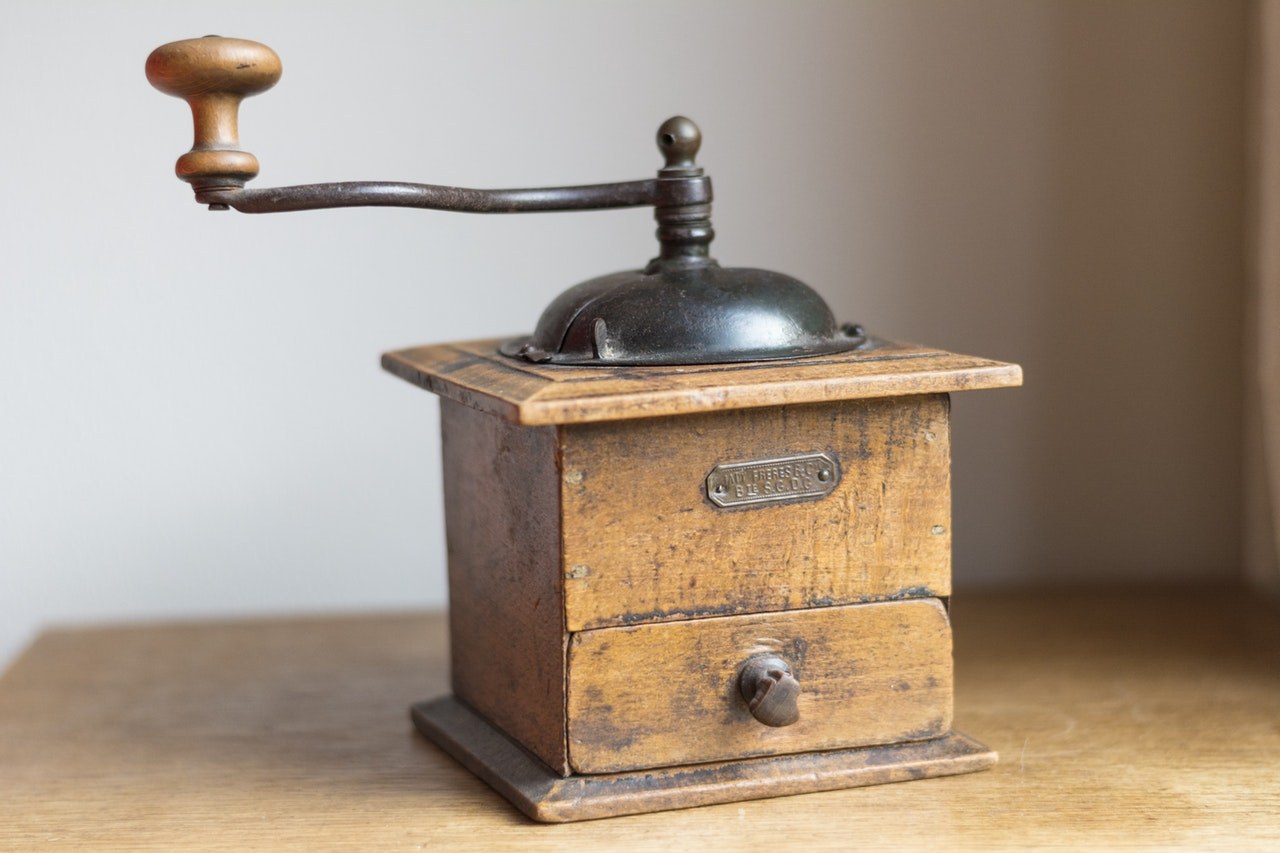
\includegraphics[width=1.0\textwidth]{../img/coffee-grinder}
\end{SlideExtra}
\fi


\begin{Slide}{Funktion: deklaration och anrop}
\SlideOnly{\setlength{\leftmargini}{0pt}}

\code{def} funktionsnamn(parameterdeklarationer): returtyp = uttryck
\vspace{0.5em}

% \begin{Code}
% def namn(param1: Typ1, param2: Typ2): Returtyp = uttryck
% \end{Code}

\begin{itemize}\SlideFontSmall
  \item En funktion har ett \Emph{huvud} och efter \code{=} kommer dess \Emph{kropp}.
  \item En \Alert{namngiven} funktion \Emph{deklareras} med nyckelordet \code{def}
  \item En funktion kan ha \Emph{parametrar} som deklareras i huvudet. 
  \item Kroppen ska vara ett uttryck (ev. ett block med flera uttryck).
  \item Parametrar binds till argument vid anrop.
  \item Uttrycket i funktionens kropp \Emph{evalueras} vid \Alert{varje anrop}. 
  \item Värdet av uttrycket blir funktionen \Emph{returvärde}. 
\end{itemize}

\pause
Exempel:
\begin{Code}
def öka(a: Int, b: Int): Int = a + b
\end{Code}
\pause
\begin{REPLnonum}
scala> öka(42, 1)
val res0: Int = 43
\end{REPLnonum}

\end{Slide}


\begin{Slide}{Deklarera funktioner, överlagring}
\begin{itemize}
\item En parameter, och sedan två parametrar:
\begin{REPL}
scala> def öka(a: Int): Int = a + 1

scala> def öka(a: Int, b: Int): Int = a + b

scala> öka(1)
val res0: Int = 2

scala> öka(1,1)
val res1: Int = 2

\end{REPL}
\item Båda funktionerna ovan kan finnas samtidigt! Trots att de har \Emph{samma namn} är de \Alert{olika funktioner}; kompilatorn kan skilja dem åt med hjälp av de \Alert{olika parameterlistorna}.

\item Detta kallas \Emph{överlagring} \Eng{overloading} av funktioner.
\item Överlagring ger flexibilitet i användningen; vi slipper hitta på nytt namn så som \code{öka2} vid 2 parametrar.
\end{itemize}
\end{Slide}



\begin{Slide}{Funktioner med defaultargument}\SlideFontSmall

\begin{itemize}
\item Vi kan ofta åstadkomma samma flexibilitet som vid överlagring, men med \Alert{en enda} funktion, om vi i stället använder \Emph{defaultargument}:
\begin{REPLnonum}
scala> def inc(a: Int, b: Int = 1) = a + b

scala> inc(42, 2)
val res0: Int = 44

scala> inc(42, 1)
val res1: Int = 43

scala> inc(42)
val res2: Int = 43

\end{REPLnonum}
\item Om ett argument utelämnas och parametern deklarerats med defaultargument så appliceras detta. Kompilatorn fyller alltså i argumentet åt oss, om det är entydigt vilken parameter som avses.
\end{itemize}
\end{Slide}


\begin{Slide}{Funktioner med namngivna argument}
\begin{itemize}
\item Genom att använda \Emph{namngivna argument} behöver man inte hålla reda på ordningen på parametrarna, bara man känner till parameternamnen.
\item Namngivna argument går fint att \Alert{kombinera} med defaultargument.
\begin{REPLnonum}[basicstyle=\SlideFontSize{7}{9}\ttfamily\color{white}]
scala> def namn(förnamn: String,
                efternamn: String,
                förnamnFörst: Boolean = true,
                ledtext: String = "Namn:"): String =
         if förnamnFörst then s"$ledtext $förnamn $efternamn"
         else s"$ledtext $efternamn, $förnamn"

scala> namn(ledtext = "Name:", efternamn = "Coder", förnamn = "Kim")
val res0: String = Name: Kim Coder
\end{REPLnonum}
\end{itemize}
\end{Slide}


\begin{Slide}{Enhetlig access}\SlideFontSmall
\begin{itemize}
\item Om en funktion \Emph{deklareras} \Alert{med} tom parameterlista \code{()} så ska den \Emph{anropas} \Alert{med} tom parameterlista.
\begin{REPLsmall}
scala> def tomParameterlista() = 42

scala> tomParameterlista()
val res1: Int = 42

scala> tomParameterlista                                                                                                                    
1 |tomParameterlista
  |^^^^^^^^^^^^^^^^^
  |method tomParameterlista must be called with () argument
\end{REPLsmall}

\item En parameterlös funktion deklarerad \Alert{utan} \code{()} ska anropas \Alert{utan} \code{()}. 
\begin{REPLsmall}
scala> def ingenParameterlista = 42
scala> ingenParameterlista()
1 |ingenParameterlista()
  |^^^^^^^^^^^^^^^^^^^
  |method ingenParameterlista does not take parameters
\end{REPLsmall}

\item Deklaration utan \code{()} möjliggör \Emph{enhetlig access}: implementationen kan ändras från \code{val} till \code{def} eller tvärtom, \Emph{utan} att \Alert{användandet} påverkas.
\pause
%\item Om parameterlista saknas får man alltså \Alert{inte} använda \code{()} vid anrop:

\end{itemize}
\end{Slide}

\Subsection{Hur ser det ut i minnet när funktioner anropas?}

\begin{Slide}{Anropsstacken och objektheapen}\SlideFontSmall
Minnet som innehåller ett programs data är uppdelat i två delar:
\begin{itemize}
\item \Emph{Anropsstacken}: 
\begin{itemize}\SlideFontSmall
\item På stackminnet läggs en \Emph{aktiveringspost} \Eng{stack frame\footnote{\href{https://en.wikipedia.org/wiki/Call_stack}{en.wikipedia.org/wiki/Call\_stack}}, activation record} för varje funktionsanrop med plats för \Alert{parametrar} och \Alert{lokala variabler}.
\item Aktiveringsposten \Alert{raderas} när \Emph{returvärdet} har levererats.
\item Stacken \Alert{växer} vid \Emph{nästlade funktionsanrop}, då en funktion i sin tur anropar en annan funktion.
\end{itemize}
\item \Emph{Objektheapen}: I heapminnet\footnote{\href{https://en.wikipedia.org/wiki/Memory_management}{en.wikipedia.org/wiki/Memory\_management}}$^{,}$\footnote{Ej att förväxlas med datastrukturen heap  \href{https://sv.wikipedia.org/wiki/Heap}{sv.wikipedia.org/wiki/Heap}} sparas alla objekt (data) som allokeras under körning. Heapen städas då och då av \Emph{skräpsamlaren} \Eng{garbage collector}, och minne som inte används längre frigörs. \\\vspace{0.5em}
%\href{http://stackoverflow.com/questions/1565388/increase-heap-size-in-java}{stackoverflow.com/questions/1565388/increase-heap-size-in-java}
% \href{https://stackoverflow.com/questions/1441373/increase-jvm-heap-size-for-scala}{stackoverflow.com/questions/1441373/increase-jvm-heap-size-for-scala}
% \begin{REPLnonum}
% scala -J-Xmx16g -J-XX:-UseGCOverheadLimit Main
% \end{REPLnonum}
\end{itemize}
\end{Slide}

% \begin{Slide}{Aktiveringspost}\SlideFontSmall
% Nästlade anrop ger växande anropsstack.
% \begin{REPL}
% scala> def f(x: Int, y: Int): Int = { val z = x + y; println(z); z}
% scala> def g(a: Int, b: Int): Int = { val c = a + b; println(c); f(c, 2 * c) }
% scala> def h(i: Int): Int = { val n = 5; g(i, i * n) }
% scala> h(2)
% \end{REPL}
%
% \pause
% \Alert{Stacken}
%
% \begin{tabular}{|r | l | l |} \hline
%
% variabel & värde & Aktiveringspost för anrop av... \\ \hline \hline
% \pause
%  i & 2 & h \\
%  n & 5 & \\ \hline
%  \pause
%  a & 2 & g \\
%  b & 10 &  \\
%  c & 12  &  \\  \hline
%  \pause
%  x & 12  & f \\
%  y & 24 &  \\
%  z & 36 & \\ \hline
% \end{tabular}
% \end{Slide}

\begin{Slide}{Aktiveringspost}\SlideFontSmall
Nästlade anrop ger växande anropsstack.
\begin{REPLsmall}
scala> def h(x: Int, y: Int) = { val z = x + y; println(z) }

scala> def g(a: Int, b: Int) = { val x = 1; h(x + 1, a + b) }

scala> def f() = { val n = 5; g(n, 2 * n) }

scala> f()

\end{REPLsmall}

\pause
\Alert{Stacken}

\begin{tabular}{|r | l | l |} \hline

variabel & värde & Aktiveringspost för anrop av... \\ \hline \hline
\pause
 n & 5 & f \\ \hline
 \pause
 a & 5 & g \\
 b & 10 &  \\
 x & 1  &  \\  \hline
 \pause
 x & 2  & h \\
 y & 15 &  \\
 z & 17 & \\ \hline
\end{tabular}
\end{Slide}

\begin{Slide}{Anropsstacken i Kojo Desktop}
Tryck på orange playknapp i Kojo och se anropsstacken.\vspace{0.5em}

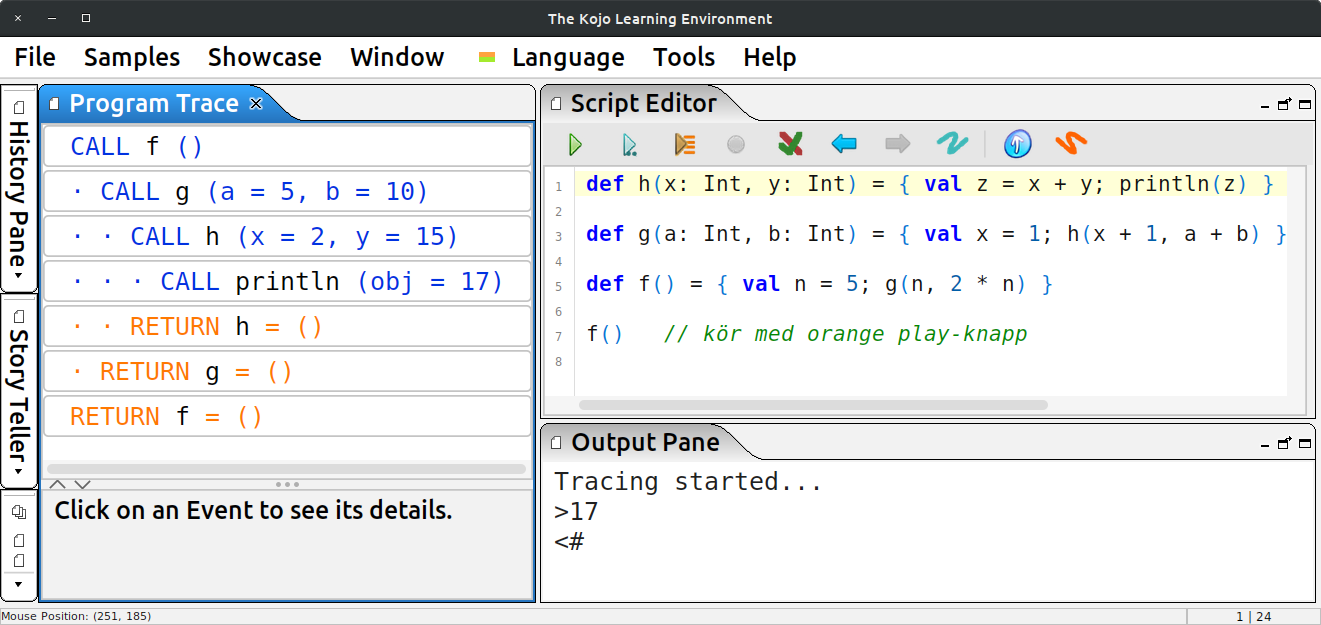
\includegraphics[width=1.0\textwidth]{../img/kojo-trace.png}  
\end{Slide}

\begin{Slide}{Anropsstacken i VS Code}
Lägg till en brytpunkt på rad 4 nedan och klicka på debug över \code{@main} i VS Code och se anropsstacken.\vspace{0.5em}

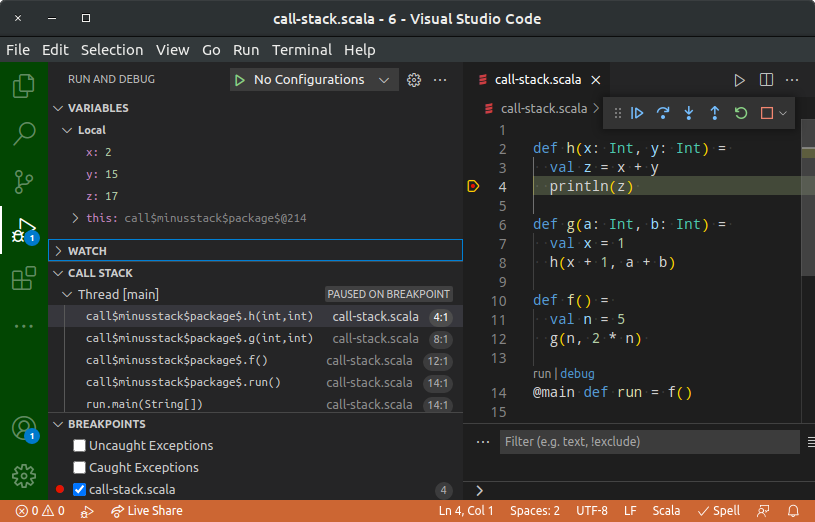
\includegraphics[width=0.85\textwidth]{../img/vscode-trace.png}  
\end{Slide}


\begin{Slide}{Vad är en stack trace?}\SlideFontSmall
När du letar buggar vid körtidsfel har du nytta av att \Alert{noga studera} \Emph{utskriften av anropsstacken} \Eng{stack trace}:
% \begin{CodeSmall}
% // Program i filen BMI.scala
% object BMI: 
%   def main(args: Array[String]): Unit = 
%     println(bmi(args(0).toInt, args(1).toInt))

%   def bmi(heightCm: Int, weightKg: Int) = 
%     safeDiv(weightKg, heightCm * heightCm) 

%   def safeDiv(numerator: Int, denominator: Int): (Int, String) = 
%     if (denominator == 0) (numerator / denominator, "ok")  // ser du buggen?
%     else (0, "division by zero") 
% \end{CodeSmall}
  
\begin{Code}[numbers=left]
// Program i filen bmi.scala

@main 
def bmi(heightCm: Int, weightKg: Int) = 
  safeDiv(weightKg, heightCm * heightCm) 

def safeDiv(numerator: Int, denominator: Int): (Int, String) = 
  if denominator == 0 then (numerator / denominator, "")  // ser du buggen?
  else (0, "division by zero")

\end{Code}
\begin{REPL}
> scalac bmi.scala 
> scala bmi 0 42
Exception in thread "main" java.lang.ArithmeticException: / by zero
        // HÄR KOMMER STACK TRACE pga körtidsfel - se nästa bild
\end{REPL}
\end{Slide}

\begin{Slide}{Hur läsa en stack trace?}
\begin{REPL}
Exception in thread "main" java.lang.ArithmeticException: / by zero
        at bmi$package$.safeDiv(bmi.scala:8)
        at bmi$package$.bmi(bmi.scala:5)
        at bmi.main(bmi.scala:3)

\end{REPL}
\begin{itemize}\SlideFontSmall
  \item En \Emph{stack trace} skrivs ut efter en krasch p.g.a. körtidsfel.
  \item Körtidsfel känns igen med ordet \Alert{Exception}.
  \item Först kommer en beskrivning av felet som orsakat kraschen, här: \\\code{java.lang.ArithmeticException: \ by zero} 
  \item Därefter visas anropsstacken.
  \item För varje funktionsanrop anges: \Emph{\texttt{klass.metod(kodfil:radnummer)}}
  \item Main-funktioner läggs i ett singelobjekt i ett speciellt paket
  \item Singelobjekt i Scala kodas som en Java-klass med dollar-tecken efter namnet, eftersom det inte finns singelobjekt i JVM.
  %\item Efter anropet av din \code{main}-procedur ligger JVM-interna anrop (\code{java.base} etc.) som du inte behöver bry dig om. %% syns inte längre i Scala 3 stack trace
\end{itemize}
\end{Slide}
  

\begin{Slide}{Lokala funktioner}\SlideFontSmall
Med lokala funktioner kan delproblem lösas med nästlade abstraktioner.

\begin{CodeSmall}
def gissaTalet(max: Int, min: Int = 1): Unit = 
  def gissat = io.StdIn.readLine(s"Gissa talet mellan $min och $max: ").toInt

  val hemlis = (math.random() * (max - min) + min).toInt

  def skrivLedtrådOmEjRätt(gissning: Int): Unit =
    if gissning > hemlis then println(s"$gissning är för stort :(")
    else if gissning < hemlis then println(s"$gissning är för litet :(")

  def inteRätt(gissning: Int): Boolean = 
    skrivLedtrådOmEjRätt(gissning)
    gissning != hemlis
  

  def loop: Int = { var i = 1; while inteRätt(gissat) do i += 1; i }

  println(s"Du hittade talet $hemlis på $loop gissningar :)")
\end{CodeSmall}

Lokala, nästlade funktionsdeklarationer är tyvärr inte tillåtna i många andra språk, t.ex. Java.\footnote{\href{http://stackoverflow.com/questions/5388584/does-java-support-inner-local-sub-methods}{\SlideFontSize{8}{9}stackoverflow.com/questions/5388584/does-java-support-inner-local-sub-methods}}

\end{Slide}

\Subsection{En funktion är ett värde}

\begin{Slide}{Funktioner är äkta värden i Scala}\SlideFontSmall
\begin{itemize}
\item En funktion är ett \Alert{äkta värde}.
\item Vi kan till exempel tilldela en variabel ett funktionsvärde.
\pause
\item Med hjälp av blank+understreck efter funktionsnamnet får vi funktionen som ett \Alert{värde} (inga argument appliceras än):
\begin{REPLnonum}
scala> def add(a: Int, b: Int) = a + b

scala> val f = add _ 
val f: (Int, Int) => Int = Lambda7210/0x0000000841e4e040@1ce2db23

scala> f(21, 21)
val res0: Int = 42
\end{REPLnonum}
\item Ett funktionsvärde har en \Alert{typ} precis som alla värden: \\
\code{f: (Int, Int) => Int}
\pause
\item Ett funktionsvärde har till skillnad från en funktionsdeklaration inget namn (variabeln \code{f} har ett namn men inte själva funktionen). Den kallas därför en \Emph{anonym} funktion eller \Alert{lambda} (mer om detta snart).
\end{itemize}
\end{Slide}

\begin{Slide}{Du kan vanligtvis skippa understreck}\SlideFontSmall
\begin{itemize}\SlideFontSmall

\item Nytt i Scala 3: Om det är otvetydigt att du vill skapa ett funktionsvärde så kan du skippa understreck:
\begin{REPLnonum}
scala> def add(a: Int, b: Int) = a + b

scala> val f = add     // inget understreck behövs 
val f: (Int, Int) => Int = Lambda7210/0x0000000841e4e040@1ce2db23
\end{REPLnonum}

\item Specialfall då understreck behövs: (se speciellt typen \code{() => Int})
\begin{REPLsmall}
scala> def a() = 42
def a(): Int

scala> val b = a
1 |val b = a
  |        ^
  |        method a must be called with () argument

scala> val b = a _
val b: () => Int = Lambda7214/0x0000000841e50440@565d794
\end{REPLsmall}
\item Börja utan understreck och se om det funkar utan kompileringsfel...
\end{itemize}
\end{Slide}

\begin{Slide}{Funktionsvärden kan vara argument}
En funktion kan ha en annan funktion som parameter:
\begin{REPL}
scala> def tvåGånger(x: Int, f: Int => Int) = f(f(x))

scala> def öka(x: Int) = x + 1

scala> def minska(x: Int) = x - 1

scala> tvåGånger(42, öka)
val res1: Int = 44

scala> tvåGånger(42, minska)
val res1: Int = 40
\end{REPL}
\end{Slide}



\begin{Slide}{Applicera funktioner på element i samlingar med \texttt{map}}\SlideFontSmall
\begin{Code}
def öka(x: Int) = x + 1

def minska(x: Int) = x - 1

val xs = Vector(1, 2, 3)
\end{Code}
\pause
Metoden \Emph{\texttt{map}} fungerar på alla Scala-samlingar och tar \Emph{en funktion som argument} och applicerar denna funktion på alla element och \Alert{skapar en ny samling} med resultaten:
\begin{REPL}
scala> xs.map(öka)
val res0: ???   // vad blir resultatet?

scala> xs.map(minska)
val res1: ???   // vad blir resultatet?
\end{REPL}
En funktion som har funktionsvärden som indata (eller utdata) kallas en\\ \Emph{högre ordningens funktion}  \Eng{higher-order function}.
\end{Slide}


\begin{Slide}{Applicera funktioner på element i samlingar med \texttt{map}}\SlideFontSmall
\begin{Code}
def öka(x: Int) = x + 1

def minska(x: Int) = x - 1

val xs = Vector(1, 2, 3)
\end{Code}
Metoden \Emph{\texttt{map}} fungerar på alla Scala-samlingar och tar \Emph{en funktion som argument} och applicerar denna funktion på alla element och \Alert{skapar en ny samling} med resultaten:
\begin{REPL}
scala> xs.map(öka)
val res0: scala.collection.immutable.Vector[Int] = Vector(2, 3, 4)

scala> xs.map(minska)
val res1: scala.collection.immutable.Vector[Int] = Vector(0, 1, 2)
\end{REPL}
En funktion som har funktionsvärden som indata kallas en\\ \Emph{högre ordningens funktion}  \Eng{higher-order function}.
\end{Slide}

\Subsection{Äkta funktioner}

\begin{Slide}{Äkta funktioner}
\begin{itemize}\SlideFontSmall
\item En \Emph{äkta} \Eng{pure} funktion är en funktion som ger ett resultat som \Alert{enbart} beror av dess argument. Alltså som funktioner i matematiken.
\item En äkta (matematisk) funktion är \Emph{referentiellt transparent} \Eng{referentially transparent}, vilket innebär att varje anrop kan bytas ut mot funktionskroppen där parametrarna ersatts med motsvarande argument.
\item En äkta funktion har \Alert{inga sidoeffekter}, t.ex. utskrift, skriva/läsa filer,  eller uppdateringar av variabler \Alert{synliga utanför} funktionen.
\item Exempel:
\begin{Code}
def add(x: Int, y: Int): Int = x + y              // äkta funktion
def rnd(n: Int): Int = (math.random() * n).toInt  // oäkta funktion
\end{Code} 
\begin{itemize}\SlideFontTiny

\item Uttrycket \code{add(41, 1)} kan ersättas med 41 +1 som i sin tur kan ersättas med 42 utan att det påverkar resultatet. Resultatet av \code{add(41, 1)} blir \Emph{samma varje gång} funktionen appliceras med dessa argument
\item Uttrycket \code{rnd(42)} kan \Alert{inte} bytas ut mot ett specifikt uttryck som säkert ger samma resultat varje gång. Alltså: \emph{ej referentiell transparens}.
\end{itemize}  
\end{itemize}  
\end{Slide}

\begin{Slide}{Exempel på oäkta funktioner: slumptal}

  \begin{itemize}
    \item Funktioner vars värden på något sätt beror av slumpen är \Alert{inte} äkta funktioner.
    \item Även om samma argument ges vid upprepad applicering, så kan ju resultatet bli olika.
    \item Studera dokumentationen för \code{scala.util.Random} här:\\ \href{https://www.scala-lang.org/api/current/scala/util/Random.html}{\SlideFontSmall https://www.scala-lang.org/api/current/scala/util/Random.html}
    \item Du har nytta av funktionen \code{Random.nextInt} och slumptalsfrö \Eng{random seed} i veckans uppgifter.
  \end{itemize}

\end{Slide}

\begin{Slide}{Slumptalsfrö: få samma slumptal varje gång}\SlideFontTiny
\begin{itemize}
\item Om man använder slumptal kan det vara svårt att leta buggar, efter som det blir \Alert{olika varje gång} man kör programmet och buggen kanske bara uppstår ibland.

\item Med klassen \code{scala.util.Random} kan man skapa \Emph{pseudo}-slumptalssekvenser.
\pause
\item Om man ger ett s.k. \Emph{frö} \Eng{seed}, av heltalstyp, som argument till konstruktorn när man skapar en instans av klassen \code{scala.util.Random}, får man samma ''slumpmässiga'' sekvens \Alert{varje gång} man kör programmet.

\begin{Code}
  val seed = 42
  val rnd = util.Random(seed) // skapa ny slumpgenerator med frö 42
  val r = rnd.nextInt(6) // ger slumptal mellan 0 till och med 5
\end{Code}
\pause
\item Om man \Alert{inte} ger ett \Emph{frö} så sätts fröet till ''\emph{a value very likely to be distinct from any other invocation of this constructor}''. Då vet vi inte vilket fröet blir och det blir olika varje gång man kör programmet.
\begin{Code}
  val rnd = util.Random() // OLIKA frö varje körning
  val r = rnd.nextInt(6) // ger slumptal mellan 0 till och med 5
\end{Code}
\pause
\end{itemize}
\end{Slide}

%\begin{Slide}{Syresättning av hjärnan vid sövande föreläsning}
%Prova nedan kod som finns här:\\
%%\href{https://github.com/lunduniversity/introprog/blob/master/compendium/examples/workspace/w05-seqalg/src/NanananananananaNanananananananaBatman.scala}{\SlideFontTiny github.com/lunduniversity/introprog/.../NanananananananaNanananananananaBatman.scala} \\
%
%
%
%\vspace{0.65em}\scalainputlisting[numbers=left,numberstyle=,basicstyle=\fontsize{6.5}{8}\ttfamily\selectfont]{../compendium/examples/workspace/w05-seqalg/src/FixSleepyBrain.scala}
%
%\pause
%Medan du lyssnar till: \href{https://www.youtube.com/watch?v=zUwEIt9ez7M}{\SlideFontSmall www.youtube.com/watch?v=zUwEIt9ez7M}\\
%Eller: \href{https://www.youtube.com/watch?v=rvXxlXg_V-k}{\SlideFontSmall www.youtube.com/watch?v=rvXxlXg\_V-k}
%\end{Slide}

\Subsection{Anonyma funktioner}


\begin{Slide}{Anonyma funktioner}
\begin{itemize}
\item  Man behöver inte ge funktioner namn. De kan i stället skapas med hjälp av \Emph{funktionsliteraler}.\footnote{Även kallat ''lambda-värde'' eller bara ''lambda'' efter den s.k. lambdakalkylen. \href{https://en.wikipedia.org/wiki/Anonymous_function}{en.wikipedia.org/wiki/Anonymous\_function}}

\item En funktionsliteral har ...
\begin{enumerate}
\item en parameterlista (utan funktionsnamn, utan returtyp),
\item sedan den reserverade teckenkombinationen \code{=>}
\item och sedan ett uttryck (eller ett block).
\end{enumerate}
\pause
\item Exempel:
\begin{Code}[basicstyle=\ttfamily\SlideFontSize{9}{11}]
(x: Int, y: Int) => x + y             // vilken typ?
\end{Code}
\pause
\item Om kompilatorn kan gissa typerna från sammanhanget så behöver typerna inte anges i själva  funktionsliteralen:
\begin{Code}[basicstyle=\ttfamily\SlideFontSize{9}{11}]
val f: (Int, Int) => Int = (x, y) => x + y
\end{Code}
\end{itemize}
\end{Slide}


\begin{Slide}{Applicera anonyma funktioner på element i samlingar}\SlideFontSmall
Anonym funktion skapad med funktionsliteral direkt i anropet:
\begin{REPL}
scala> val xs = Vector(1, 2, 3)

scala> xs.map((x: Int) => x + 1)
res0: scala.collection.immutable.Vector[Int] = Vector(2, 3, 4)
\end{REPL}
\pause
Eftersom kompilatorn här kan härleda typerna så behövs de inte:
\begin{REPL}
scala> xs.map(x => x + 1)
res1: scala.collection.immutable.Vector[Int] = Vector(2, 3, 4)
\end{REPL}
\pause
Om man bara använder parametern en enda gång i funktionen så kan man byta ut parameternamnet mot ett understreck.
\begin{REPL}
scala> xs.map(_ + 1)
res2: scala.collection.immutable.Vector[Int] = Vector(2, 3, 4)
\end{REPL}
\end{Slide}



\begin{Slide}{Platshållarsyntax för anonyma funktioner}\SlideFontSmall
Understreck i funktionsliteraler kallas \Emph{platshållare} \Eng{placeholder} och medger ett förkortat skrivsätt \Alert{om} den parameter som understrecket representerar används \Alert{endast en gång}.
\begin{Code}[basicstyle=\ttfamily\fontsize{10}{12}\selectfont]
_ + 1
\end{Code}
Ovan expanderas av kompilatorn till följande funktionsliteral \\(där namnet på parametern är godtyckligt):
\begin{Code}[basicstyle=\ttfamily\fontsize{10}{12}\selectfont]
x => x + 1
\end{Code}
\pause
Det kan förekomma flera understreck; det första avser första parametern, det andra avser andra parametern etc.
\begin{Code}[basicstyle=\ttfamily\fontsize{10}{12}\selectfont]
_ + _
\end{Code}
\pause
... expanderas till:
\begin{Code}[basicstyle=\ttfamily\fontsize{10}{12}\selectfont]
(x, y) => x + y
\end{Code}
\end{Slide}


\begin{Slide}{Exempel på platshållarsyntax med \texttt{reduceLeft}}\SlideFontSmall
Metoden \code{reduceLeft} applicerar en funktion på de två första elementen i en sekvens och tar sedan resultatet som första argument och nästa element som andra argument och upprepar detta genom hela samlingen.
\begin{REPL}
scala> def summa(x: Int, y: Int) = x + y

scala> val xs = Vector(1, 2, 3, 4, 5)

scala> xs.reduceLeft(summa)
res20: Int = 15

scala> xs.reduceLeft((x, y) => x + y)
res21: Int = 15

scala> xs.reduceLeft(_ + _)
res22: Int = 15

scala> xs.reduceLeft(_ * _)
res23: Int = 120
\end{REPL}
\end{Slide}


\begin{Slide}{Predikat, med och utan namn}
\begin{itemize}\SlideFontSmall
\item En funktion som har \code{Boolean} som returtyp kallas för ett \Emph{predikat}. 
\item Exempel:
\begin{Code}
def isTooLong(name: String): Boolean = name.length > 10

def isTall(heightInMeters: Double, limit: Double = 1.78): Boolean = 
  heightInMeters > limit
\end{Code}
\item Predikat ges ofta ett namn som börjar på \code{is} eller \code{has} så att man lätt kan se att det är ett predikat när man läser kod som anropar funktionen.
\item Många av samlingsmetoderna i Scalas standardbibliotek tar predikat som funktionsargument. Exempel med predikat som anonym funktion: 
\begin{REPLnonum}
scala> val parts = Vector(3, 1, 0, 5).partition(_ > 1)
val parts: (Vector[Int], Vector[Int]) = 
  (Vector(3, 5),Vector(1, 0))
\end{REPLnonum} 
\item Studera snabbreferensen och försök hitta samlingsmetoder som tar predikat som funktionsargument. \url{http://cs.lth.se/pgk/quickref} \\I anropsexempel med predikat-argument används bokstaven \code{p}.
\end{itemize}  
\end{Slide}


\Subsection{Skapa din egen kontrollstruktur}  

\begin{Slide}{Hur fungerar egentligen \code{upprepa} i Kojo?}
\begin{Code}[basicstyle=\ttfamily\SlideFontSize{14}{16}]
upprepa(10) {
  println("hej")
}
\end{Code}

\pause
Vi ska nu se hur vi, genom att kombinera ett antal koncept, kan skapa egna kontrollstrukturer likt upprepa ovan:
\begin{itemize}
\item klammerparentes vid ensam paramenter
\item multipla parameterlistor
\item namnanrop (fördröjd evaluering)
\end{itemize}
\end{Slide}



\begin{Slide}{Multipla parameterlistor}
Vi har tidigare sett att man kan ha mer än en parameter:
\begin{REPLnonum}
scala> def add(a: Int, b: Int) = a + b

scala> add(21, 21)
res0: Int = 42
\end{REPLnonum}
Man kan även ha \Alert{mer än en} \Emph{parameterlista}:
\begin{REPLnonum}
scala> def add(a: Int)(b: Int) = a + b

scala> add(21)(21)
res1: Int = 42
\end{REPLnonum}
\Eng{multiple parameter lists}

\href{http://docs.scala-lang.org/style/declarations.html#multiple-parameter-lists}{\SlideFontTiny docs.scala-lang.org/style/declarations.html\#multiple-parameter-lists}
\end{Slide}



\begin{Slide}{Värdeanrop och namnanrop}\SlideFontSmall
Det vi sett hittills är \Emph{värdeanrop}: argumentet evalueras \Alert{först} innan dess \Alert{värde} \emph{sedan} appliceras:
\begin{REPL}
scala> def byValue(n: Int): Unit = for i <- 1 to n do print(" " + n)

scala> byValue(21 + 21)
 42 42 42 42 42 42 42 42 42 42 42 42 42 42 42 42 42 42 42 42 42 42 42 42 42 42 42 42 42 42 42 42 42 42 42 42 42 42 42 42 42 42

scala> byValue({print(" hej"); 21 + 21})
 hej 42 42 42 42 42 42 42 42 42 42 42 42 42 42 42 42 42 42 42 42 42 42 42 42 42 42 42 42 42 42 42 42 42 42 42 42 42 42 42 42 42 42
\end{REPL}
\pause
Men man kan med \code{=>} före parametertypen åstadkomma \Emph{namnanrop}: argumentet \Alert{''klistras in''} i stället för \Alert{namnet} och evalueras \Alert{varje gång} (kallas även \Emph{fördröjd evaluering}):
\begin{REPL}
scala> def byName(n: => Int): Unit = for i <- 1 to n do print(" " + n)

scala> byName({print(" hej"); 21 + 21})
 hej hej 42 hej 42 hej 42 hej 42 hej 42 hej 42 hej 42 hej 42 hej 42 hej 42 hej 42 hej 42 hej 42 hej 42 hej 42 hej 42 hej 42 hej 42 hej 42 hej 42 hej 42 hej 42 hej 42 hej 42 hej 42 hej 42 hej 42 hej 42 hej 42 hej 42 hej 42 hej 42 hej 42 hej 42 hej 42 hej 42 hej 42 hej 42 hej 42 hej 42 hej 42 hej 42
\end{REPL}
\Alert{Kluring}: Varför skrivs ''hej'' ut en extra gång i början? \pause ledtråd: \texttt{1 to \Alert{n}}
%evalueringen av n i 1 to n ger ett extra hej
\end{Slide}

\begin{Slide}{Klammerparenteser vid ensam parameter}
Så här har vi sett nyss att man man göra:
\begin{REPL}
scala> def twice(action: => Unit): Unit = { action; action }

scala> twice( { print("hej"); print("san ") } )
hejsan hejsan
\end{REPL}

Det ser rätt klyddigt ut med \code+{(+  och \code+)}+ eller vad tycker du? \pause Men...
För alla funktioner \code{f} gäller att: \\ det är helt ok att byta ut vanliga parenteser: \hfill\code{f(uttryck)} \\ mot krullparenteser: \hfill\code|f{uttryck}| \\ \Alert{om} parameterlistan har \Alert{exakt en} parameter.

\vspace{0.5em}Man kan alltså skippa det yttre parentesparet för bättre läsbarhet:
\begin{REPLnonum}
scala> twice { print("hej"); print("san ") }
\end{REPLnonum}
\end{Slide}



\begin{Slide}{Skapa din egen kontrollstruktur}
\begin{itemize}
\item Genom att \Alert{kombinera} \Emph{multipla parameterlistor} med \Emph{namnanrop} med \Emph{klammerparentes vid ensam parameter} kan vi skapa vår egen kontrollstruktur: \code{upprepa} \pause
\begin{Code}
upprepa(42){
  if math.random() < 0.5 then print(" gurka")
  else print(" tomat")
}
\end{Code}
Hur då?
\pause
 Till exempel så här:
\begin{Code}
def upprepa(n: Int)(block: => Unit) = 
  for i <- 0 until n do block
\end{Code}

\pause

\begin{REPLnonum}
gurka gurka gurka tomat tomat gurka gurka gurka gurka tomat tomat tomat tomat tomat
\end{REPLnonum}
\end{itemize}
\end{Slide}


\begin{Slide}{Stegade funktioner, ''Curry-funktioner''}
Om en funktion har multipla parameterlistor kan man skapa \Emph{stegade funktioner}, även kallat \Emph{partiellt applicerade} funktioner \Eng{partially applied functions} eller \Emph{''Curry''-funktioner}.
\begin{REPLnonum}
scala> def add(x: Int)(y: Int) = x + y

scala> val öka = add(1)
val öka: Int => Int = Lambda7339/0x0000000841eb7040@19c8add7

scala> Vector(1,2,3).map(öka)
val res0: Vector[Int] = Vector(2, 3, 4)

scala> Vector(1,2,3).map(add(2))
val res1: Vector[Int] = Vector(3, 4, 5)
\end{REPLnonum}
\end{Slide}


\begin{Slide}{Funktion med fångad variabelrymd: \textit{closure}}
\begin{Code}
def f(x: Int): Int => Int = 
  val a = 42 + x
  def g(y: Int): Int = y + a
  g
\end{Code}
Funktionen \code{g} \Alert{fångar} den lokala variabeln \code{a} i ett \Emph{funktionsobjekt}.
\pause
\begin{REPLnonum}
scala> val funkis = f(1)
val funkis: Int => Int = Lambda7356/0x0000000841ed2840@1bda26bc

scala> funkis(2)
val res0: Int = 45
\end{REPLnonum}
\pause
Ett funktionsobjekt med ''fångade'' variabler kallas \Alert{closure}. \\
(Mer om funktioner som objekt senare.)
\end{Slide}

\ifkompendium\else
\begin{SlideExtra}{Översikt av begrepp vi gått igenom hittills}
\begin{enumerate}
\item överlagring
\item utelämna tom parameterlista (enhetlig access)
\item defaultargument
\item namngivna argument
\item lokala funktioner
\item funktioner som äkta värden
\item anonyma funktioner
\item klammerparentes vid ensam paramenter
\item multipla parameterlistor
\item namnanrop (fördröjd evaluering)
\item egendefinierade kontrollstrukturer
\item stegade funktioner (''Curry-funktioner'')
\item fångad variablelrymd i funktionsobjekt (''closure'')
\end{enumerate}
\end{SlideExtra}
\fi



\Subsection{Kort om rekursion}

\begin{Slide}{Rekursiva funktioner}
\begin{itemize}
\item Funktioner som \Alert{anropar sig själv} kallas \Emph{rekursiva}.


\begin{REPLnonum}
scala> def fakultet(n: Int): Int =
         if n < 2 then 1 else n * fakultet(n - 1)

scala> fakultet(5)
val res0: Int = 120
\end{REPLnonum}

\item För varje nytt anrop läggs en ny aktiveringspost på stacken.

\item I aktiveringsposten sparas varje returvärde som gör att \code{5 * (4 * (3 * (2 * 1)))} kan beräknas.

\item Rekrusionen avbryts när man når \Emph{basfallet}, här \code{n < 2}

\item En rekursiv funktion \Alert{måste} ha en returtyp.

\end{itemize}

\end{Slide}

\begin{Slide}{Loopa med rekursion}
\begin{Code}
def gissaTalet(max: Int, min: Int = 1): Unit =
  def gissat = 
    io.StdIn.readLine(s"Gissa talet mellan [$min, $max]: ").toInt

  val hemlis = (math.random() * (max - min) + min).toInt

  def skrivLedtrådOmEjRätt(gissning: Int): Unit =
    if gissning > hemlis then println(s"$gissning är för stort :(")
    else if (gissning < hemlis) println(s"$gissning är för litet :(")

  def ärRätt(gissning: Int): Boolean = 
    skrivLedtrådOmEjRätt(gissning)
    gissning == hemlis

  def loop(n: Int = 1): Int = if ärRätt(gissat) then n else loop(n + 1)

  println(s"Du hittade talet $hemlis på ${loop()} gissningar :)")
\end{Code}
\end{Slide}


\begin{Slide}{Rekursiva datastrukturer}
\begin{itemize}
\item Datastrukturena Lista och Träd är exempel på datastrukturer som passar bra ihop med rekursion.
\item Båda dessa datastrukturer kan beskrivas rekursivt:
\begin{itemize}
\item En lista består av ett huvud och en lista, som i sin tur består av ett huvud och en lista, som i sin tur...
\item Ett träd består av grenar till träd som i sin tur består av grenar till träd som i sin tur, ...
\end{itemize}
\item Dessa datastrukturer bearbetas med fördel med rekursiva algoritmer.
\item I denna kursen ingår rekursion endast ''för kännedom'': \\ du ska veta vad det är och kunna skapa en enkel rekursiv funktion, t.ex. fakultets-beräkning. Du kommer jobba mer med rekursion och rekursiva datastrukturer i fortsättningskursen.
\end{itemize}
\end{Slide}

\Subsection{Automatisera kompilering: byggverktyg}

\begin{Slide}{Bygga applikationer}
\begin{itemize}
  \item Den kreativa programmeringsprocessen innehåller många korta cykler av koda, ändra, testa.
  \item Det blir många omkompileringar och då vill man gärna slippa skriva samma kommando om och om igen. En lösning är att skapa ett skript, t.ex. i språket \Emph{bash}, som kör kompileringen.
  \item  Om man bara gör en liten ändring vill man bara kompilera om det som ändrats och inte kompilera om rubbet varje gång. En lösning på detta problem är att använda ett \Emph{byggverktyg}, t.ex. Scala Build Tool (\code{sbt}), se Appendix F.

\end{itemize}
\end{Slide}

\begin{Slide}{Bash-skript för kompilering}\SlideFontSmall
\begin{itemize}
  \item Det gamla skriptspråket \Emph{bash} funkar i Linux och MacOS.
  \item Bash är smidigt för enkla program som använder terminalkommando, men syntaxen är knepig och det finns många fallgropar.
  \item I ett bash-skript kan du t.ex. kompilera och köra ett program. Exempel i filen \code{build.sh} nedan:
\begin{Code}
scalac mitt-program.scala && scala MinMain
\end{Code}
Med pil-upp kan du enkelt kompilera om efter varje ändring:
\begin{REPLnonum}
> sh build.sh
\end{REPLnonum}
  \item Det går att få \Emph{bash} och ubuntu-terminalen att funka i Windows 10 med WSL (Windows Linux Subsystem) där du kan välja Ubuntu 18.04 LTS: \\
  {\SlideFontTiny\url{https://docs.microsoft.com/en-us/windows/wsl/install-win10}}
\end{itemize}
{\noindent   Det finns dock stora begränsningar med WSL och om du vill ha Linux ''på riktigt'' rekommenderas att du installera Ubuntu med dual-boot: \SlideFontTiny\url{https://linoxide.com/distros/install-ubuntu-18-04-dual-boot-windows-10/}}
\end{Slide}

\begin{Slide}{Scala Build Tool: \texttt{sbt}}
\begin{itemize}
  \item Ett byggverktyg, t.ex. \code{sbt}, kan användas för att kompilera, testköra, ladda ner, paketer, distribuera programbibliotek och applikationer.
  \item Det är mycket enkelt att använda \code{sbt} för att kompilera och köra om ditt program varje gång du sparar din fil, tex. med \code{Ctrl+S} så här:
\begin{REPLnonum}
> sbt
sbt> ~run   // tecknet ~ ger omkörning vid ändring
\end{REPLnonum}
Tecknet \code{~} kallas \emph{tilde} och skrivs med högra Alt-tangenten nere och två tryck på tangenten bredvid Enter.
  \item LTH:s datorer har \code{sbt} förinstallerat. Ladda ner till din dator: \\
  \url{https://www.scala-sbt.org/download.html}
  \item Läs mer om byggverktyg i Appendix F.

\end{itemize}

\end{Slide}




\ifkompendium\else
\Subsection{Veckans uppgifter}

\begin{SlideExtra}{Mål med övning \ExeWeekTHREE}
\begin{itemize}\SlideFontSmall
  %!TEX encoding = UTF-8 Unicode
%!TEX root = ../exercises.tex

\item Kunna skapa och använda funktioner med en eller flera parametrar, default-argument, och namngivna argument.
\item Kunna förklara nästlade funktionsanrop med aktiveringsposter på stacken.
\item Kunna förklara skillnaden mellan äkta och ''oäkta'' funktioner.
\item Kunna applicera en funktion på alla element i en samling.

\item Kunna använda funktioner som äkta värden.
\item Kunna skapa och använda anonyma funktioner (ä.k. lambda-funktioner).

\item Känna till att funktioner kan ha uppdelad parameterlista.
\item Känna till att det går att partiellt applicera argument på funktioner med uppdelad parameterlista för att skapa s.k. stegade funktioner (ä.k. curry-funktioner).

\item Känna till rekursion och kunna beskriva vad som kännetecknar en rekursiv funktion.
%\item Känna till att man kan loopa med rekursion och att svansrekursiva funktioner kan optimeras till while-loopar.

\item Känna till att det går att skapa egna kontrollstrukturer med hjälp av namnanrop.
\item Känna till skillnaden mellan värdeanrop och namnanrop.
\item Kunna tolka en stack trace.

\end{itemize}
\end{SlideExtra}

\begin{SlideExtra}{Mål med laboration \LabWeekTHREE}
\begin{itemize}
  %!TEX encoding = UTF-8 Unicode
%!TEX root = ../compendium2.tex

%\item Kunna kompilera Scalaprogram med \texttt{scalac}.
%\item Kunna köra Scalaprogram med \texttt{scala}.
%\item Kunna definiera och anropa funktioner.
%\item Kunna använda och förstå default-argument.
%\item Kunna ange argument med parameternamn.
\item Kunna skapa ett större program med din egen kod efter dina egna idéer.
\item Kunna använda en editor och terminalen för att iterativt editera, kompilera, och testa din kod.
\item Kunna använda variabler i kombination med alternativ och repetetition i flera nivåer.
\item Kunna stegvis förbättra din kod för att underlätta förändring och öka läsbarhet.
\item Kunna skapa och använda abstraktioner för att generalisera och möjliggöra återanvändning av kod.

\end{itemize}
Ni ska spela \Emph{varandras} textspel i din \Alert{samarbetsgrupp}.\\
Läs labbinstruktioner:\url{http://cs.lth.se/pgk/compendium/}
\end{SlideExtra}


\begin{SlideExtra}{Tips till ditt textspel.}
\begin{CodeSmall}
"Yes".toLowerCase.startsWith("y")    // true
"hejsan".contains("ejsa")            // true
"42".toInt                           // 42
"?".toIntOption.getOrElse(42)        // 42
Thread.sleep(1000)                   // ger lagom irriterande fördröjning (1 sekund)

val i = 42
s"Livets mening är $i!" // dollar $ före namn vid stränginterpolering med s""
s"Livets mening är inte ${i-1}!"  // klamrar ${} vid evaluering av uttryck

"""|en sträng som spänner över
   |flera rader där marginalen fram till vertikalstreck
   |är bortplockad med stripMargin (kan kombineras med s-interpolatorn)
""".stripMargin

math.random() < 0.8                  // true i 80% av fallen
scala.util.Random.nextInt(42)      // ger slumptal mellan 0 och 41
scala.io.StdIn.readLine("prompt>") // ger sträng som användaren skriver

val x = try { "?".toInt } catch { case e: Exception => 42 }  // förhindrar krasch
Thread.sleep(1000)    // sova i 1000 milliskeunder
\end{CodeSmall}
Kolla \Emph{snabbreferensen} vad mer du kan göra med strängar!
\end{SlideExtra}

\begin{SlideExtra}{Exempel på en början till ett textspel}
  Här finns en exempel på en enkel \emph{början} på ett textspel som du stegvis kan ändra och bygga ut till något du själv vill göra:
  \url{https://github.com/lunduniversity/introprog/tree/master/workspace/w03_irritext}

\begin{itemize}
  \item Vilka begrepp och principer ger koden träning i?
\end{itemize}

\end{SlideExtra}

\begin{SlideExtra}{Jobba så här}
\begin{itemize}
  \item Skriv koden i en editor.
  \item Ha ett terminalfönster med \code{sbt} där du kör \code{~compile} eller \code{~run} så att din kod kompileras eller körs om varje gång du sparar.
  \item Ha ett terminalfönster med en fristående scala REPL där du kan göra mindre undersökningar rad för rad.
  \item Börja enkelt och bygg vidare steg för steg.
  \item Bygg om koden allteftersom den växer genom att införa nya abstraktioner med väl valda namn (s.k. ''refaktorisering'') .
  \item Fixa \Alert{alla} kompileringsfel \code{||} körtidsfel \Emph{innan} du går vidare.
  \item Fokusera på kodens \Alert{läsbarhet}.
\end{itemize}

\end{SlideExtra}

\fi


%!TEX encoding = UTF-8 Unicode
%!TEX root = ../exercises.tex

\ifPreSolution

\Exercise{\ExeWeekTHREE}\label{exe:W03}
\begin{Goals}
%!TEX encoding = UTF-8 Unicode
%!TEX root = ../exercises.tex

\item Kunna skapa och använda funktioner med en eller flera parametrar, default-argument, och namngivna argument.
\item Kunna förklara nästlade funktionsanrop med aktiveringsposter på stacken.
\item Kunna förklara skillnaden mellan äkta och ''oäkta'' funktioner.
\item Kunna applicera en funktion på alla element i en samling.

\item Kunna använda funktioner som äkta värden.
\item Kunna skapa och använda anonyma funktioner (ä.k. lambda-funktioner).

\item Känna till att funktioner kan ha uppdelad parameterlista.
\item Känna till att det går att partiellt applicera argument på funktioner med uppdelad parameterlista för att skapa s.k. stegade funktioner (ä.k. curry-funktioner).

\item Känna till rekursion och kunna beskriva vad som kännetecknar en rekursiv funktion.
%\item Känna till att man kan loopa med rekursion och att svansrekursiva funktioner kan optimeras till while-loopar.

\item Känna till att det går att skapa egna kontrollstrukturer med hjälp av namnanrop.
\item Känna till skillnaden mellan värdeanrop och namnanrop.
\item Kunna tolka en stack trace.

\end{Goals}

\begin{Preparations}
\item \StudyTheory{03}
\end{Preparations}

\BasicTasks %%%%%%%%%%%%%%%%

\else

\ExerciseSolution{\ExeWeekTHREE}

\fi





\WHAT{Para ihop begrepp med beskrivning.}

\QUESTBEGIN

\Task \what

\vspace{1em}\noindent Koppla varje begrepp med den (förenklade) beskrivning som passar bäst:

\begin{ConceptConnections}
  funktionshuvud & 1 & & A & fördröjd evaluering av argument \\ 
  funktionskropp & 2 & & B & koden som exekveras vid funktionsanrop \\ 
  parameterlista & 3 & & C & funktion utan namn; kallas även lambda \\ 
  block & 4 & & D & gör att argument kan ges i valfri ordning \\ 
  namngivna argument & 5 & & E & en funktion som anropar sig själv \\ 
  defaultargument & 6 & & F & gör att en funktion kan flera resultatvärden \\ 
  värdeanrop & 7 & & G & har parameterlista och eventuellt returtyp \\ 
  namnanrop & 8 & & H & kan ha lokala namn; sista raden ger värdet \\ 
  tupel & 9 & & I & lista med bestämt antal (heterogena) värden \\ 
  tupelreturtyp & 10 & & J & argumentet evalueras innan anrop \\ 
  äkta funktion & 11 & & K & ger alltid samma resultat om samma argument \\ 
  slumptalsfrö & 12 & & L & beskriver namn och typ på parametrar \\ 
  anonym funktion & 13 & & M & gör att argument kan utelämnas \\ 
  rekursiv funktion & 14 & & N & om lika blir sekvensen av pseudoslumptal samma \\ 
\end{ConceptConnections}

\SOLUTION

\TaskSolved \what

\begin{ConceptConnections}
  funktionshuvud & 1 & ~~\Large$\leadsto$~~ &  M & har parameterlista och eventuellt en returtyp \\ 
  funktionskropp & 2 & ~~\Large$\leadsto$~~ &  L & koden som exekveras vid funktionsanrop \\ 
  parameterlista & 3 & ~~\Large$\leadsto$~~ &  I & beskriver namn och typ på parametrar \\ 
  block & 4 & ~~\Large$\leadsto$~~ &  E & kan ha lokala namn; sista raden ger värdet \\ 
  namngivna argument & 5 & ~~\Large$\leadsto$~~ &  J & gör att argument kan ges i valfri ordning \\ 
  defaultargument & 6 & ~~\Large$\leadsto$~~ &  F & gör att argument kan utelämnas \\ 
  värdeanrop & 7 & ~~\Large$\leadsto$~~ &  C & argumentet evalueras innan anrop \\ 
  namnanrop & 8 & ~~\Large$\leadsto$~~ &  K & fördröjd evaluering av argument \\ 
  äkta funktion & 9 & ~~\Large$\leadsto$~~ &  A & ger alltid samma resultat om samma argument \\ 
  predikat & 10 & ~~\Large$\leadsto$~~ &  G & en funktion som ger ett booleskt värde \\ 
  slumptalsfrö & 11 & ~~\Large$\leadsto$~~ &  B & ger återupprepningsbar sekvens av pseudoslumptal \\ 
  anonym funktion & 12 & ~~\Large$\leadsto$~~ &  D & funktion utan namn; kallas även lambda \\ 
  rekursiv funktion & 13 & ~~\Large$\leadsto$~~ &  H & en funktion som anropar sig själv \\ 
\end{ConceptConnections}

\QUESTEND





\WHAT{Definiera och anropa funktioner.}

\QUESTBEGIN

\Task \label{task:funcall} \what~
En funktion med en parameter definieras med följande syntax i Scala:
\vspace{0.5em} \\
\texttt{\code{def} \textit{namn}(\textit{parameter}: \textit{Typ} = \textit{defaultArgument}): \textit{Returtyp} = \textit{returvärde}}

% En funktion med två parametrar definieras med följande syntax i Scala: \vspace{0.5em} \\  \texttt{\code{def} \textit{namn}(\textit{parameter1}: \textit{Typ1}, \textit{parameter2}: \textit{Typ2}): \textit{Returtyp} = \textit{returvärde}}

\Subtask Definiera en funktionen \code{öka} som har en heltalsparameter \code{x} och vars returvärde är argumentet plus 1. Defaultargument ska vara 1. Ange returtypen explicit.

\Subtask Vad har uttrycket \code{öka(öka(öka(öka())))} för värde?

\Subtask Definiera funktionen \code{minska} som har en heltalsparameter \code{x} och vars returvärde är argumentet minus 1. Defaultargument ska vara 1. Ange returtypen explicit.

\Subtask Vad är värdet av uttrycket \code{öka(minska(öka(öka(minska(minska())))))}

\Subtask Vad är det för skillnad mellan parameter och argument?

\SOLUTION

\TaskSolved \what

\SubtaskSolved
\begin{Code}
def öka(x: Int = 1): Int = x + 1
\end{Code}

\SubtaskSolved  \code{4}

\SubtaskSolved
\begin{Code}
def minska(x: Int = 1): Int = x - 1
\end{Code}

\SubtaskSolved  \code{0}

\SubtaskSolved
\begin{itemize}
  \item \emph{Kort, förenklad förklaring:} Parametern i funktionshuvudet är ett lokalt namn på indata som kan användas i funktionskroppen, medan argumentet är själva värdet på parametern som skickas med vid anrop.
  \item \emph{Längre, mer exakt förklaring:} En \textbf{parameter} är en deklaration av en oföränderlig variabel i ett funktionshuvud vars namn finns tillgängligt lokalt i funktionskroppen. Vid anrop \emph{binds} parameternamnet till ett specifikt argument. Ett \textbf{argument} är ett uttryck som  appliceras på en funktion vid anrop. Normalt evalueras argumentet innan anropet sker, men om parametertypen föregås av \code{=>} fördröjs evalueringen av argumentet och sker i stället \emph{varje gång} parameternamnet förekommer i funktionskroppen.
\end{itemize}

\QUESTEND




\WHAT{Textspelet AliensOnEarth.}

\QUESTBEGIN

\Task  \what~Ladda ner spelet nedan \footnote{
\url{https://raw.githubusercontent.com/lunduniversity/introprog/master/compendium/examples/AliensOnEarth.scala}} och studera koden.

\scalainputlisting[basicstyle=\ttfamily\fontsize{10.5}{12.5}\selectfont,numbers=left]{examples/AliensOnEarth.scala}

% def randomDistribution(weights: Vector[Int]): Int = {
%   require(weights.size > 0)
%   require(weights.forall(_ >= 0))
%
%   val probabilities = for (w <- weights) yield w / weights.sum.toDouble
%   val rnd = math.random
%   var i = 0
%   var sum = probabilities(i)
%   while (i < probabilities.size - 1 && rnd > sum) {
%     i += 1
%     sum += probabilities(i)
%   }
%   i
% }

\Subtask Medan du läser koden, försök lista ut vilket som är bästa strategin för att få så mycket poäng som möjligt. Kompilera och kör spelet i terminalen med ditt favoritnamn som argument. Vilket av de tre objekten på planeten jorden har störst sannolikhet att vara bästa alternativet?

\Subtask Para ihop kodsnuttarna nedan med bästa beskrivningen.\footnote{Gör så gott du kan även om allt inte är solklart. Vissa saker kommer vi att gå igenom i detalj först under senare kursmoduler.}

\begin{ConceptConnections}
  \code|options.indices| & 1 & & A & slumptal i intervallet \code|0 until n| \\ 
  \code|"1X2".toLowercase| & 2 & & B & fångar undantag för att förhindra krasch \\ 
  \code|Random.nextInt(n)| & 3 & & C & gör om en sträng till små bokstäver \\ 
  \code|try { } catch { }| & 4 & & D & skriver ut information om ett undantag \\ 
  \code|""" ... """| & 5 & & E & heltalssekvens med alla index i en sekvens \\ 
  \code|s.stripMargin| & 6 & & F & sträng som kan sträcka sig över flera kodrader \\ 
  \code|e.printStackTrace| & 7 & & G & tar bort marginal till och med vertikalstreck \\ 
\end{ConceptConnections}

\noindent\emph{Tips:} Med hjälp av REPL kan du ta reda på hur olika delar fungerar, t.ex.:

\begin{REPL}
scala> val os = Vector("p", "w", "a")
scala> os.indices
scala> os.indices.foreach(i => println(i))
scala> os.indexOf("w")
scala> os.indexOf("gurka")
scala> Vector("hej", "hejsan", "hej").indexOf("hej")
scala> try { 1 / 0 } catch { case e: Exception=> println(e) }
\end{REPL}
Kolla även dokumentationen för \code{nextInt}, \code{readLine}, m.fl genom att söka
här: \\ \url{http://www.scala-lang.org/api/current/index.html}


\begin{framed}
\noindent\emph{Tips inför fortsättningen:}

\begin{itemize}[nolistsep]
  \item När jag hittade på \code{AliensOnEarth} började jag med ett mycket litet program med en enkel \code{main}-funktion som bara skrev ut något kul. Sedan byggde jag vidare på programmet steg för steg och kompilerade och testade efter varje liten ändring.

  \item När jag kodar har jag REPL igång i ett eget terminalfönster och api-dokumentationen för Scala i en webbläsare redo för sökningar. Jag återanvänder också användbara snuttar från kod jag gjort tidigare och inspireras ofta av lösningar från \url{https://stackoverflow.com} (om jag kan begripa dem och de verkar rimliga).

  \item Detta arbetssätt tar ett tag att komma in i, men är ett bra sätt att uppfinna allt större och bättre program. Ett stort program byggs lättast i små inkrement och felsökning blir mycket lättare om man bara gör små tillägg åt gången.

  \item Du får också det mycket lättare att förstå ditt program om du delar upp koden i många korta funktioner med bra namn. Du kan sedan lättare hitta på mer avancerade funktioner genom att återanvända befintliga.

  \item Under veckans laboration ska du utveckla ditt eget textspel. Då har du nytta av att återanvända funktionerna för indata och slumpdragning från \code{AliensOnEarth}.
\end{itemize}

\end{framed}


\SOLUTION

\TaskSolved \what~

\SubtaskSolved \code{"penguin"} är bästa alternativ med sannolikheten $\frac{1}{2} + \frac{1}{2}\cdot\frac{1}{3} = \frac{2}{3}$

\SubtaskSolved

\begin{ConceptConnections}
    \code|options.indices| & 1 & ~~\Large$\leadsto$~~ &  D & heltalssekvens med alla index i en sekvens \\ 
  \code|"1X2".toLowercase| & 2 & ~~\Large$\leadsto$~~ &  C & gör om en sträng till små bokstäver \\ 
  \code|Random.nextInt(n)| & 3 & ~~\Large$\leadsto$~~ &  G & slumptal i intervallet \code|0 until n| \\ 
  \code|try { } catch { }| & 4 & ~~\Large$\leadsto$~~ &  A & fångar undantag för att förhindra krasch \\ 
  \code|""" ... """| & 5 & ~~\Large$\leadsto$~~ &  B & sträng som kan sträcka sig över flera kodrader \\ 
  \code|s.stripMargin| & 6 & ~~\Large$\leadsto$~~ &  F & tar bort marginal till och med vertikalstreck \\ 
  \code|e.printStackTrace| & 7 & ~~\Large$\leadsto$~~ &  E & skriver ut information om ett undantag \\ 
\end{ConceptConnections}

\QUESTEND



\WHAT{Äkta funktioner.}

\QUESTBEGIN

\Task  \what~  En äkta funktion%
\footnote{Äkta funktioner uppfyller per definition  \textit{referentiell transparens} \Eng{referential transparency} som du kan läsa mer om här:  \href{https://en.wikipedia.org/wiki/Referential_transparency}{en.wikipedia.org/wiki/Referential\_transparency}}
\Eng{pure function} ger alltid samma resultat med samma argument (så som vi är vana vid inom matematiken) och har inga externt observerbara sidoeffekter (till exempel utskrifter).

Vilka funktioner i objektet \code{inSearchOfPurity} nedan är äkta funktioner?
\begin{Code}
object inSearchOfPurity {
  var x = 0
  val y = x
  def inc(i: Int): Int = i + 1
  def oink(i: Int): String = { x = x + i; "Pig says " + ("oink " * x) }
  def addX(i: Int): Int = x + i
  def addY(i: Int): Int = y + i
  def isPalindrome(s: String): Boolean = s == s.reverse
  def rnd(min: Int, max: Int): Double = math.random * max + min
}
\end{Code}


\noindent\emph{Tips:} Klistra in hela singelobjektet i REPL och testa att anropa funktionerna om du är osäker på vad som händer. Om du gör \code{import inSearchOfPurity._} kommer du åt namnen i singelobjektet direkt och kan lätt undersöka variablernas värden.

\SOLUTION

\TaskSolved \what

\begin{itemize}
  \item Funktionerna  \code{inc}, \code{addY} och \code{isPalindrome} är äkta. Notera att \code{y}-variablen initialiseras till \code{0} och kan sedan inte ändras eftersom den är deklarerad med nyckelordet \code{val}.
\end{itemize}

\QUESTEND




\WHAT{Funktioner är objekt med en \code{apply}-metod.}

\QUESTBEGIN

\Task  \what~ \\
\noindent Vilka rader nedan ger kompileringsfel?

\begin{REPL}
scala> object plus { def apply(x: Int, y: Int) = x + y }
scala> plus.apply(42, 43)
scala> plus.apply(42)
scala> plus(42, 43)
scala> plus(42)
\end{REPL}


\SOLUTION

\TaskSolved \what

\begin{itemize}
  \item Rad 3 och 5 ger kompileringsfelet\\
  \texttt{error: not enough arguments for method apply}
\end{itemize}

\QUESTEND



\WHAT{Applicera funktion på varje element i en samling. Funktion som argument.}

\QUESTBEGIN

\Task  \what~

\noindent Deklarera funktionen \code{öka} och variabeln \code{xs} enligt nedan i REPL:
\begin{REPL}
scala> def öka(x: Int) = x + 1
scala> val xs = Vector(3, 4, 5)
\end{REPL}
\noindent Para ihop nedan uttryck till vänster med det uttryck till höger som har samma värde. Om du undrar något, testa uttrycken och olika varianter av dem i REPL.

\begin{ConceptConnections}
  \code|for (i <- 1 to 3) yield öka(i)| & 1 & & A & \code|Vector(5, 6, 7)| \\ 
  \code|Vector(2, 3, 4).map(i => öka(i))| & 2 & & B & \code|()| \\ 
  \code|xs.map(öka)| & 3 & & C & \code|xs| \\ 
  \code|xs.map(öka).map(öka)| & 4 & & D & \code|Vector(2, 3, 4)| \\ 
  \code|xs.foreach(öka)| & 5 & & E & \code|Vector(4, 5, 6)| \\ 
\end{ConceptConnections}

\SOLUTION

\TaskSolved \what

\begin{ConceptConnections}
    \code|for (i <- 1 to 3) yield öka(i)| & 1 & ~~\Large$\leadsto$~~ &  C & \code|Vector(2, 3, 4)| \\ 
  \code|Vector(2, 3, 4).map(i => öka(i))| & 2 & ~~\Large$\leadsto$~~ &  E & \code|xs| \\ 
  \code|xs.map(öka)| & 3 & ~~\Large$\leadsto$~~ &  B & \code|Vector(4, 5, 6)| \\ 
  \code|xs.map(öka).map(öka)| & 4 & ~~\Large$\leadsto$~~ &  D & \code|Vector(5, 6, 7)| \\ 
  \code|xs.foreach(öka)| & 5 & ~~\Large$\leadsto$~~ &  A & \code|()| \\ 
\end{ConceptConnections}

\QUESTEND



\WHAT{Funktion som äkta värde.}

\QUESTBEGIN

\Task  \what~  Funktioner är \emph{äkta värden} i Scala\footnote{I likhet med t.ex. Javascript, men till skillnad från t.ex. Java.}. Det betyder att variabler kan ha funktioner som värden och funktionsvärden kan vara argument till funktioner som har funktionsparametrar\footnote{Funktioner som tar funktioner som argument kallas \emph{högre ordningens funktioner}}.

  En funktion som har en heltalsparameter och ett heltalsresultat är av funktionstypen \code{Int => Int} (uttalas \emph{int-till-int}) och värdet av funktionen utgör ett objekt som har en metod som heter \code{apply} med motsvarande funktionstyp.

\Subtask \label{subtask:funcval} Deklarera nedan funktioner och variabler i REPL. Notera understrecket på rad 3. Para sedan ihop nedan uttryck till vänster med det uttryck till höger som har samma värde. Om du undrar något, testa uttrycken och olika varianter av dem i REPL.

\begin{REPL}
scala> def öka(x: Int): Int = x + 1
scala> def app(x: Int, f: Int => Int): Int = f(x)
scala> val f1 = öka _
scala> var f2 = (x: Int) => x - 1
\end{REPL}

\begin{ConceptConnections}
  \code| öka(-1)     | & 1 & & A & \code| 1     | \\ 
  \code| app(1, öka) | & 2 & & B & \code| 0     | \\ 
  \code| app(5, f2)  | & 3 & & C & \code| 3     | \\ 
  \code| f1(2)       | & 4 & & D & \code| öka(1)| \\ 
  \code| f2(2)       | & 5 & & E & \code| 4     | \\ 
\end{ConceptConnections}


\Subtask Vilka typer har variablerna \code{f1} och \code{f2}?

\Subtask Går det att ge variabeln \code{f2} funktionsvärdet \code{öka} genom tilldelning?

\Subtask Går det bra att skriva \code{val f3 = öka} utan understreck?

\Subtask Går det bra att skriva \code{val f3: Int => Int = öka} utan understreck?

\SOLUTION

\TaskSolved \what

\SubtaskSolved

\begin{ConceptConnections}
    \code| öka(-1)     | & 1 & ~~\Large$\leadsto$~~ &  C & \code| 0     | \\ 
  \code| app(1, öka) | & 2 & ~~\Large$\leadsto$~~ &  A & \code| öka(1)| \\ 
  \code| app(5, f2)  | & 3 & ~~\Large$\leadsto$~~ &  E & \code| 4     | \\ 
  \code| f1(2)       | & 4 & ~~\Large$\leadsto$~~ &  B & \code| 3     | \\ 
  \code| f2(2)       | & 5 & ~~\Large$\leadsto$~~ &  D & \code| 1     | \\ 
\end{ConceptConnections}

\SubtaskSolved Båda har typen \code{Int => Int}

\SubtaskSolved  Ja, det går fint.

\SubtaskSolved  Nej det blir kompileringsfel: \\
\begin{REPL}
scala> val f3 = öka
<console>:12: error: missing argument list for method öka
Unapplied methods are only converted to functions when
a function type is expected. You can make this conversion
explicit by writing 'öka _' or 'öka(_)' instead of 'öka'.
\end{REPL}

\SubtaskSolved  Ja, det går fint. Nu med typinformationen på plats är kompilatorn säker på vad du vill göra.

\QUESTEND




\WHAT{Anonyma funktioner.}

\QUESTBEGIN

\Task  \what~  Vi har flera gånger sett syntaxen \code{i => i + 1}, till exempel i en loop \code{(1 to 10).map(i => i + 1)} där funktionen \code{i => i + 1} appliceras på alla heltal från 1 till och med 10 och resultatet blir en ny sekvenssamling.

Syntaxen \code{(i: Int) => i + 1} är en litteral för att skapa ett funktionsvärde. Syntaxen liknar den för funktionsdeklarationer, men nyckelordet \code{def} saknas i funktionshuvudet och i stället för likhetstecken används \code{=>} för att avskilja parameterlistan från funktionskroppen.
Om kompilatorn kan härleda typen ur sammanhanget kan kortformen \code{i => i + 1} användas.

Det finns ett \emph{ännu} kortare sätt att skriva en anonym funktion \emph{om} typen kan härledas \emph{och} den bara använder sin parameter \emph{en enda gång}; då går funktionslitteraler att skriva med s.k. platshållarsyntax som använder understreck, till exempel \code{ _ + 1} och som automatiskt expanderas av kompilatorn till \code{ngtnamn => ngtnamn + 1} (namnet på parametern spelar ingen roll; kompilatorn väljer något eget, internt namn).

Para ihop uttryck till vänster med uttryck till höger som har samma värde:

\begin{ConceptConnections}
  \code|(0 to 2).map(i => i + 1)           | & 1 & & A & \code|Vector(9.0, 16.0, 25.0) | \\ 
  \code|(1 to 3).map(_ + 1)                | & 2 & & B & \code|Vector(4.0, 8.0, 16.0)  | \\ 
  \code|(2 to 4).map(math.pow(2, _))       | & 3 & & C & \code|Vector(2.0, 2.5, 3.0)   | \\ 
  \code|(3 to 5).map(math.pow(_, 2))       | & 4 & & D & \code|Vector(2, 3, 4)         | \\ 
  \code|(4 to 6).map(_.toDouble).map(_ / 2)| & 5 & & E & \code|(2 to 4).map(i => i - 1)| \\ 
\end{ConceptConnections}

\noindent
Funktionslitteraler kallas även \textit{anonyma funktioner}\footnote{Ett annat populärt men mer kryptiskt namn är \textit{lambda}.}, eftersom de inte har något namn, till skillnad från t.ex. \code{def öka(i: Int): Int = i + 1}, som ju heter \code{öka}.

\SOLUTION

\TaskSolved \what

\begin{ConceptConnections}
    \code|(0 to 2).map(i => i + 1)           | & 1 & ~~\Large$\leadsto$~~ &  C & \code|(2 to 4).map(i => i - 1)| \\ 
  \code|(1 to 3).map(_ + 1)                | & 2 & ~~\Large$\leadsto$~~ &  B & \code|Vector(2, 3, 4)         | \\ 
  \code|(2 to 4).map(math.pow(2, _))       | & 3 & ~~\Large$\leadsto$~~ &  E & \code|Vector(4.0, 8.0, 16.0)  | \\ 
  \code|(3 to 5).map(math.pow(_, 2))       | & 4 & ~~\Large$\leadsto$~~ &  A & \code|Vector(9.0, 16.0, 25.0) | \\ 
  \code|(4 to 6).map(_.toDouble).map(_ / 2)| & 5 & ~~\Large$\leadsto$~~ &  D & \code|Vector(2.0, 2.5, 3.0)   | \\ 
\end{ConceptConnections}

\QUESTEND





\ExtraTasks %%%%%%%%%%%%%%%%%%%%%%%%%%%%%%%%%%%%%%%%%%%%%%%%%%%%%%%%%%




\WHAT{Funktion med flera parametrar.}

\QUESTBEGIN

\Task  \what~  Definiera i REPL två funktioner \code{sum} och \code{diff} med två heltalsparametrar som returnerar summan respektive differensen av argumenten: \\
\code{def sum(x: Int, y: Int): Int = x + y} \\
\code{def diff(x: Int, y: Int): Int = x - y} \\
Vad har nedan uttryck för värden? Förklara vad som händer.

\Subtask \code{diff(0, 100)}

\Subtask \code{diff(100, sum(42, 43))}

\Subtask \code{sum(sum(42, 43), diff(100, sum(0, 0)))}

\Subtask \code{sum(diff(Byte.MaxValue, Byte.MinValue),1)}

\SOLUTION

\TaskSolved \what

\SubtaskSolved  \code{-100}

\SubtaskSolved  \code{15}

\SubtaskSolved  \code{185}

\SubtaskSolved  \code{256}

\QUESTEND



\WHAT{Medelvärde.}

\QUESTBEGIN

\Task  \what~ Skriv och testa en funktion \code{avg} som räknar ut medelvärdet mellan två heltal och returnerar en \code{Double}.

\SOLUTION

\TaskSolved \what

\begin{Code}
def avg(x: Int, y: Int): Double = (x + y) / 2.0
\end{Code}

\QUESTEND




\WHAT{Funktionsanrop med namngivna argument.}

\QUESTBEGIN

\Task  \what~
\begin{REPL}
scala> def skrivNamn(efternamn: String, förnamn: String) =
         println(s"Namn: $efternamn, $förnamn")
scala> skrivNamn(förnamn = "Stina", efternamn = "Triangelsson")
scala> skrivNamn(efternamn = "Oval", "Viktor")

\end{REPL}

\Subtask Vad skrivs ut efter rad 3 resp. rad 4 ovan?

\Subtask Nämn tre fördelar med namngivna argument.

\SOLUTION

\TaskSolved \what~

\SubtaskSolved
\begin{REPL}
Namn: Triangelsson, Stina
Namn: Oval, Viktor
\end{REPL}

\SubtaskSolved
\begin{itemize}
  \item Anroparen kan själv välja ordning.
  \item Koden blir lättare att begripa om parameternamnen är självbeskrivande.
  \item Hjälper till att förhindra buggar som beror på förväxlade parametrar.
\end{itemize}

\QUESTEND




\WHAT{Bortkastade resultatvärden och returtypen \code{Unit}.}

\QUESTBEGIN

\Task  \what~ Undersök nedan kod i REPL och förklara vad som händer.

\Subtask
\begin{REPL}
scala> def tom = println("")
scala> println(tom)
\end{REPL}

\Subtask
\begin{REPL}
scala> def bortkastad: Unit = 1 + 1
scala> println(bortkastad)
\end{REPL}

\Subtask
\begin{REPL}
scala> def bortkastad2 = { val x = 1 + 1 }
scala> println(bortkastad2)
\end{REPL}

\Subtask Varför är det bra att explicit ange \code{Unit} som returtyp för procedurer?

\SOLUTION

\TaskSolved \what

\SubtaskSolved Procedurer returnerar tomma värdet och \code{println} är en procedur.

\SubtaskSolved Proceudrer returnerar tomma värdet. Om du anger returtyp \code{Unit} explicit, har du bättre chans att kompilatorn kan ge varning då uträkningar kommer att kastas bort.

\SubtaskSolved I Scala är variabeldeklaratin, precis som en tilldelningssats, och inte ett uttryck och saknar värde.

\SubtaskSolved  Koden blir lättare att läsa och kompilatorn får bättre möjlighet att hjälpa till med varningar om resultatvärden riskerar att bli bortkastade.

\QUESTEND




\AdvancedTasks %%%%%%%%%%%%%%%%%%%%%%%%%%%%%%%%%%%%%%%%%%%%%%%%%%%%%%%%%%%




\WHAT{Föränderlighet av parametrar.}

\QUESTBEGIN

\Task \what~Är en parameter förändringsbar i funktionskroppen ...

\Subtask ... i Scala?  (Ja/Nej)

\Subtask ... i Java?  (Ja/Nej)

\SOLUTION

\TaskSolved \what~

\Subtask Nej, i Scala är parametern oföränderlig och det blir kompileringsfel om man försöker tilldela den ett nytt värde i funktionskroppen.

\Subtask Ja det går utmärkt i Java att ändra värdet på parametern i funktionskroppen med tilldelning, men koden riskerar att bli förvirrande.\\
\url{https://stackoverflow.com/questions/2970984}

\QUESTEND




\WHAT{Rekursion.}

\QUESTBEGIN

\Task  \what~  En rekursiv funktion anropar sig själv.

\Subtask Förklara vad som händer nedan.

\begin{REPL}
scala> def countdown(x: Int): Unit = if (x > 0) {println(x); countdown(x -1)}
scala> countdown(10)
scala> countdown(-1)
scala> def finalCountdown(x: Byte): Unit =
         {println(x); Thread.sleep(100); finalCountdown((x-1).toByte); 1 / x}
scala> finalCountdown(Byte.MaxValue)
\end{REPL}

\Subtask Vad händer om du gör satsen som riskerar division med noll \emph{före} det rekursiva anropet i funktionen \code{finalCountdown} ovan?

\Subtask Förklara vad som händer nedan. Varför tar sista raden längre tid än näst sista raden?
\begin{REPL}
scala> def signum(a: Int): Int = if (a >= 0) 1 else -1
scala> def add(x: Int, y: Int): Int =
         if (y == 0) x else add(x + 1, y - signum(y))
scala> add(100,100)
scala> add(Int.MaxValue, 0)
scala> add(0, Int.MaxValue)
\end{REPL}

\SOLUTION

\TaskSolved \what

\SubtaskSolved
\code{countdown} skriver ut x och kallar på \code{countdown} igen med x-1 som argument om det är större än noll vilket innebär att samma sak görs igen tills x når 0.

\code{finalCountdown} gör samma sak fast med en Byte och den fortsätter även om x passerar 0 med de rekursiva funktionsanropen.

\SubtaskSolved
Eftersom vi hade \code{1/x} efter rekursionsanropet innan så kom vi aldrig dit för vi returnerade aldrig något utan gick bara djupare i stacken. Om vi placerar \code{1/x} tidigare så når vi den raden kod och den kastar ett exception då det är division med noll.

\SubtaskSolved
Den sista raden leder till mycket fler rekursiva anrop, för rekursionen avslutas när y är noll, inte om x är det.

\QUESTEND




\WHAT{Undersök svansrekursion genom att kasta undantag.}

\QUESTBEGIN

\Task  \what~  Förklara vad som händer. Kan du hitta bevis för att kompilatorn kan optimera rekursionen till en vanlig loop?

\begin{REPL}
scala> def explode = throw new Exception("BANG!!!")
scala> explode
scala> lastException.printStackTrace
scala> def countdown(n: Int): Unit =
         if (n == 0) explode else countdown(n-1)
scala> countdown(10)
scala> lastException.printStackTrace
scala> def countdown2(n: Int): Unit =
         if (n == 0) explode else {countdown2(n-1); print("no tailrec")}
scala> countdown2(10)
scala> countdown2(1000)
scala> lastException
scala> lastException.getStackTrace.size
scala> :javap countdown
scala> :javap countdown2
\end{REPL}

\SOLUTION

\TaskSolved \TODO %% TODO

\QUESTEND



\WHAT{\code{@tailrec}-annotering.}

\QUESTBEGIN

\Task  \what~  Du kan be kompilatorn att ge felmeddelande om den inte kan optimera koden till motsvarande en while-loop. Om den inte kan det hämmas prestanda och det finns risk för en överfull stack \Eng{stack overflow}. Prova nedan rader i REPL och förklara vad som händer.
\begin{REPL}
scala> def countNoTailrec(n: Long): Unit =
         if (n <= 0L) println("Klar! " + n) else {countNoTailrec(n-1L); ()}
scala> countNoTailrec(1000L)
scala> countNoTailrec(100000L)
scala> import scala.annotation.tailrec
scala> @tailrec def countNoTailrec(n: Long): Unit =
         if (n <= 0L) println("Klar! " + n) else {countNoTailrec(n-1L); ()}
scala> @tailrec def countTailrec(n: Long): Unit =
         if (n <= 0L) println("Klar! " + n) else countTailrec(n-1L)
scala> countTailrec(1000L)
scala> countTailrec(100000L)
scala> countTailrec(Int.MaxValue.toLong * 2L)
\end{REPL}\SOLUTION

\QUESTEND



\WHAT{Uppdelad parameterlista. \TODO}

\QUESTBEGIN

\Task  \what~Man kan dela upp parametrarna till en funktion i flera parameterlistor. Förklara vad som händer här:
\begin{REPL}
scala> def add(a: Int)(b: Int) = a + b
scala> add(22)(20)
scala> add(22)(add(1)(19))
\end{REPL}

\SOLUTION

\TaskSolved \what

Först så adderas 22 och 20 för att bli 42.
Sedan adderas först 1 och 19 och det adderas sen med 22 för att till slut bli 42.

\QUESTEND




\WHAT{Stegade funktioner (''Curry-funktioner''). \TODO}

\QUESTBEGIN

\Task  \what~ Förklara vad som händer nedan.
\begin{REPL}
scala> def sum(a: Int)(b: Int) = a + b
scala> sum(1)(2)
scala> val f = sum(42) _
scala> f(1)
scala> val inc = sum(1) _
scala> val dec = sum(-1) _
scala> inc(42)
scala> dec(42)
\end{REPL}

\SOLUTION

\TaskSolved \what
 När man gör curryfunktioner så skjuter man upp att ange det andra värdet till senare och på så sätt gör "nya" funktioner så att säga. När vi sparar undan variablen \code{f} så har vi angett första argumentet men den väntar fortfarande på det andra som vi anger sen vilket ger ett resultatvärde.

Samma sak senare, genom att skapa variablerna inc och dec som summan av +1 respektive -1 så har vi "skapat" våra \code{inc} och \code{dec} funktioner från tidigare funktioner.

\QUESTEND

%!TEX encoding = UTF-8 Unicode
%!TEX root = ../compendium2.tex

\Lab{\LabWeekTHREE}
\begin{Goals}
%!TEX encoding = UTF-8 Unicode
%!TEX root = ../compendium2.tex

%\item Kunna kompilera Scalaprogram med \texttt{scalac}.
%\item Kunna köra Scalaprogram med \texttt{scala}.
%\item Kunna definiera och anropa funktioner.
%\item Kunna använda och förstå default-argument.
%\item Kunna ange argument med parameternamn.
\item Kunna skapa ett större program med din egen kod efter dina egna idéer.
\item Kunna använda en editor och terminalen för att iterativt editera, kompilera, och testa din kod.
\item Kunna använda variabler i kombination med alternativ och repetetition i flera nivåer.
\item Kunna stegvis förbättra din kod för att underlätta förändring och öka läsbarhet.
\item Kunna skapa och använda abstraktioner för att generalisera och möjliggöra återanvändning av kod.

\end{Goals}

\begin{Preparations}
\item \DoExercise{\ExeWeekTWO}{02}
\item \DoExercise{\ExeWeekTHREE}{03}
\end{Preparations}



\subsection{Obligatoriska uppgifter}


\begin{quote}
\textbf{Blockmullvad} (\textit{Talpa laterculus}) är ett fantasidjur i familjen mullvadsdjur.
Den är känd för sitt karaktäristiska kvadratiska utseende.
Den lever mest ensam i sina underjordiska gångar som till skillnad från mullvadens (\emph{Talpa europaea}) har helt raka väggar.
\end{quote}

\begin{figure}
\end{figure}

\Task
Du ska skriva ett Scala-program med en vanlig texteditor och kompilera ditt program med kommandot \texttt{scalac} och sedan köra programmet med kommandot \texttt{scala}.

\Subtask
Öppna en texteditor, till exempel gedit eller Atom (se appendix~\ref{appendix:edit} för hjälp).
Skapa en ny fil med namnet \texttt{Mole.scala} och spara den i en ny katalog i din hemkatalog, till exempel \texttt{\textasciitilde/pgk/mole/Mole.scala}, där \texttt{\textasciitilde} är din hemkatalog.

\Subtask
Öppna ett terminalfönster (se appendix~\ref{appendix:terminal} för hjälp).
Navigera till din nya katalog med \texttt{cd}-kommandot \Eng{change directory} och kontrollera med \texttt{ls}-kommandot \Eng{list} att din nya fil finns där.
\begin{REPLnonum}
> cd ~/pgk/mole
> ls
\end{REPLnonum}
Om allt går bra ska \texttt{ls}-kommandot skriva ut \texttt{Mole.scala}.

\Subtask
Gå tillbaka till din texteditor och skriv in ett objekt med namnet \code{Mole} i din fil.
Lägg till en \code{main}-funktion i objektet som skriver ut texten \emph{Keep on digging!} med hjälp av funktionen \code{println}.
Behöver du hjälp kan du gå tillbaka till övningarna i kapitel~\ref{exe:W03}.

\Subtask
Kör kommandot \texttt{scalac Mole.scala} i terminalfönstret för att kompilera ditt program.
Om kompilatorn rapporterar några fel rättar du till det i din texteditor kompilerar igen.
Kontrollera sedan med \texttt{ls}-kommandot att några filer som slutar på \texttt{class} har skapats.

\Subtask
Kör kommandot \texttt{scala Mole} för att köra ditt program.
Om att går bra ska texten du angivit skrivas ut i terminalfönstret.


\Task
Nu har du skrivit ett Scala-program som skriver ut en uppmaning till en mullvad att fortsätta gräva.
Det programmet är inte så användbart, eftersom mullvadar inte kan inte läsa.
Nästa steg är att skriva ett grafiskt program, snarare än ett textbaserat.

Funktionen \code{println} som anropas i \code{main}-funktionen ingår i Scalas standardbibliotek.
Ett programbibliotek innehåller kod eller kompilerade programsnuttar som kan användas av andra program, och för de flesta programspråk ingår ett standardbibliotek som alla program kan nyttja.
Till grafiken i denna uppgift ska du använda ett bibliotek som kallas \emph{cslib} och som kommer att användas även i senare labbar.

\Subtask

Ladda ner \texttt{cslib.jar} via länken \url{http://cs.lth.se/pgk/cslib} och lägg jar-filen i samma katalog som ditt Scala-program.
En jar-fil används för att paketera färdigkompilerade program, kod, dokumentation, resursfiler, etc, och är komprimerad på samma sätt som en zip-fil.

\Subtask
Byt ut \code{main}-funktionens kropp mot följande block:
\begin{Code}
{
	val w = new cslib.window.SimpleWindow(300, 500, "Digging")
	w.moveTo(10, 10)
	w.lineTo(10, 20)
	w.lineTo(20, 20)
	w.lineTo(20, 10)
	w.lineTo(10, 10)
}
\end{Code}
Den första raden skapar ett nytt \code{SimpleWindow} som ritar upp ett fönster som är 300 bildpunkter brett och 500 bildpunkter högt med titeln \emph{Digging}.
\code{SimpleWindow} har en \emph{penna} som kan flyttas runt och rita linjer.
Anropet \code{w.moveTo(10, 10)} flyttar pennan för fönstret \code{w} till position $(10,10)$ utan att rita något, och anropet \code{w.lineTo(10, 20)} ritar en linje därifrån till position $(10, 20)$.

\Subtask
Nu ska du kompilera ditt program, men eftersom \code{SimpleWindow} inte finns i Scalas standardbibliotek utan i \texttt{cslib.jar} behöver du visa kompilatorn var den ska leta.
Det gör du genom att ange en \emph{classpath}, dvs. en sökväg till \texttt{class}-filer, när du kompilerar.
Använd flaggan \texttt{-cp cslib.jar} för att ange \texttt{cslib.jar} som classpath och kompilera ditt Scala-program igen:
\begin{REPLnonum}
> scalac -cp cslib.jar Mole.scala
\end{REPLnonum}

\Subtask
Nu ska du köra ditt program, och då behöver du också ange var \texttt{class}-filerna ligger.
Du ska ange den katalog där \texttt{class}-filerna för \code{Mole} ligger, som du just kompilerat, men du ska också ange \texttt{cslib.jar}, och det gör du med en kolon-separerad lista\footnote{Kolon används i Linux och macOS, medan Windows använder semikolon.}, till exempel \code{"sökväg1:sökväg2:sökväg3"}.
Katalogen du står i, där dina \texttt{class}-filer ligger, kan anges med en punkt (\texttt{.}).
Kör programmet med följande kommando (om Windows använd semikolon):
\begin{REPLnonum}
> scala -cp ".:cslib.jar" Mole
\end{REPLnonum}
Du ska nu få upp ett fönster med en liten kvadrat utritad i övre vänstra hörnet.


\Task
Hela ditt program är för tillfället samlat i en och samma funktion, vilket fungerar bra för väldigt små program.
Nu ska vi strukturera programmet så det blir lättare att återanvända samma kodsnuttar.

\Subtask
Lägg till ett objekt med namnet \code{Graphics} i \texttt{Mole.scala} och flytta dit deklarationen av fönstret \code{w}.
Skapa en ny funktion med namnet \code{square} i det nya objektet och flytta dit koden som ritar kvadraten.
Anropa \code{square} i din \code{main}-funktion.
Filen \texttt{Mole.scala} ska se ut såhär (förutom \code{???}):
\begin{Code}
object Graphics {
	val w = new cslib.window.SimpleWindow(300, 500, "Digging")
	def square(): Unit = ???
}
object Mole {
	def main(args: Array[String]): Unit = {
		Graphics.square()
	}
}
\end{Code}
Observera att du inte kan anropa \code{square} direkt i funktionen \code{main}, utan måste ange att det är \code{square}-funktionen inuti \code{Graphics} du vill anropa.

\Subtask
Kompilera \texttt{Mole.scala} med \texttt{scalac}.
Glöm inte att ange korrekt classpath.
(\emph{Tips:} Du kan trycka uppåtpil för att komma till tidigare kommandon i terminalen.)
Kontrollera med \texttt{ls} att det nu också finns \texttt{class}-filer för \code{Graphics}-objektet.

\Subtask
Kör programmet \code{Mole} med \texttt{scala}.
Glöm inte att ange korrekt classpath.
Om allt fungerar ska programmet göra samma sak som innan.

\Task
Nu har du gjort ett grafiskt program, men ännu syns ingen mullvad.
Det är dags att ta reda på hur koordinatsystemet fungerar i denna grafiska miljö, så vi kan få mullvaden att hitta rätt.

\Subtask
Ändra i \code{Graphics.square} så att kvadraten ritas upp i \emph{övre högra} hörnet istället.
Prova dig fram för att ta reda på hur koordinatsystemet fungerar genom att ändra i koden, kompilera och köra programmet tills du får rätt på det.

\Subtask\Checkpoint
Visa kvadraten för din labbhandledare och förklara vad de två parametrarna gör genom att peka ut ungefär var positionerna $(0,0)$, $(300, 0)$, $(0, 300)$ och $(300, 300)$ ligger.

\Subtask
Ta bort anropet till funktionen \code{square} när du har visat den för din labbhandledare.

\Task
Nu ska du skapa ett nytt koordinatsystem för \code{Graphics} som har \emph{stora} bildpunkter.
Vi kallar \code{Graphics} stora bildpunkter för \emph{block} för att lättare skilja dem från \code{SimpleWindow}s bildpunkter.
Om blockstorleken är $b$, så ligger koordinaten $(x, y)$ i \code{Graphics} på koordinaten $(bx, by)$ i \code{SimpleWindow}.

\Subtask
Lägg till följande deklarationer överst i objektet \code{Graphics}.
\begin{Code}
val width = 30
val height = 50
val blockSize = 10
\end{Code}
Ändra bredden på ditt \code{SimpleWindow} till \code{width * blockSize} och ändra höjden till \code{height * blockSize}.

\Subtask
Skapa en ny funktion i \code{Graphics} med namnet \code{block} och två parametrar \code{x} och \code{y} av typen \code{Int} och returtypen \code{Unit}.
Metodens \emph{kropp} ska se ut såhär:
\begin{Code}
{
    val left = x * blockSize
    val right = left + blockSize - 1
    val top = y * blockSize
    val bottom = top + blockSize - 1

    for (row <- top to bottom) {
      w.moveTo(left, row)
      w.lineTo(right, row)
    }
}
\end{Code}

\Subtask\Pen
Metoden \code{block} ritar ett antal linjer.
Hur många linjer ritas ut?
I vilken ordning ritas linjerna?

\Subtask
Anropa funktionen \code{Graphics.block} några gånger i \code{Mole.main} så att några block ritas upp i fönstret när programmet körs.
Kompilera och kör ditt program.


\Task
Det finns många sätt att beskriva färger.
I naturligt språk har vi olika namn på färgerna, till exempel \emph{vitt}, \emph{rosa} och \emph{magenta}.
I datorn är det vanligt att beskriva färgerna som en blandning av \emph{rött}, \emph{grönt} och \emph{blått} i det så kallade RGB-systemet.
\code{SimpleWindow} använder typen \code{java.awt.Color} för att beskriva färger och \code{java.awt.Color} bygger på RGB.
Det finns några fördefinierade färger i \code{java.awt.Color}, till exempel \code{java.awt.Color.black} för svart och \code{java.awt.Color.green} för grönt.
Andra färger kan skapas genom att ange mängden rött, grönt och blått.

\Subtask
Skapa ett nytt objekt i \texttt{Mole.scala} med namnet \code{Colors} och lägg in följande definitioner:
\begin{Code}
val mole = new java.awt.Color(51, 51, 0)
val soil = new java.awt.Color(153, 102, 51)
val tunnel = new java.awt.Color(204, 153, 102)
\end{Code}
% val sky = new java.awt.Color(51, 51, 204)
% val grass = new java.awt.Color(51, 204, 51)
Den tre parametrarna till \code{new java.awt.Color(r, g, b)} anger hur mycket \emph{rött}, \emph{grönt} respektive \emph{blått} som färgen ska innehålla, och mängderna ska vara i intervallet 0--255.
Färgen $(153, 102, 51)$ innebär ganska mycket rött, lite mindre grönt och ännu mindre blått och det upplevs som brunt.
Objektet \code{Colors} är en färgpallett, men vi har inte ritat något med färg ännu.
Kompilera och kör ditt program ändå, för att se så programmet fungerar likadant som sist.

\Subtask
Lägg till en parameter till \code{Graphics.block} sist i parameterlistan med namnet \code{color} och typen \code{java.awt.Color}.
Låt \emph{default-argumentet} för den nya parametern vara \code{java.awt.Color.black}.
(Kommer du inte ihåg hur man gör default-argument kan du titta på övningarna i kapitel~\ref{exe:W03}.)
För att ändra färgen på blocket kan du byta linjefärg innan du ritar.
Lägg till följande rad i början på \code{Graphics.block}:
\begin{Code}
w.setLineColor(color)
\end{Code}
Kompilera och kör ditt program igen för att se om det fortfarande fungerar.

\Subtask\Pen
Funktionen \code{Graphics.block} har tre parametrar, men den anropas bara med två parametrar i \code{Mole.main}.
Varför är det tillåtet?
Vilket värde har den tredje parametern om ingen anges?

\Subtask
Ändra i \code{Mole.main} och lägg till en av definitionerna från objektet \code{Colors} som tredje parameter till \code{Graphics.block}.
Kompilera och kör ditt program och upplev världen i färg.

\Task
I programmet används många långa namn med punkter, som till exempel \code{java.awt.Color} och \code{Graphics.block}.
Dessa punkt-separerade namn kallas \emph{kvalificerade} namn.
För att slippa skriva dessa långa namn hela tiden kan man \emph{importera} en definition och sen använda bara den sista delen av namnet.

\Subtask
Importera namnet \code{java.awt.Color} i objektet \code{Colors}. Ändra sen alla \code{new java.awt.Color(...)} i objektet till \code{new Color(...)}.
(Har du glömt hur man importerar ett namn kan du gå tillbaka till övningarna i kapitel~\ref{exe:W02}.)

\Subtask\Pen
I vilka av objekten \code{Mole}, \code{Colors} och \code{Graphics} kan du använda det korta respektive det kvalificerade namnet av \code{java.awt.Color}?

\Subtask
Importera namnet \code{java.awt.Color} så att det korta namnet \code{Color} kan användas i objekten \code{Colors} och \code{Graphics} men inte i \code{Mole}.
Byt sedan ut de långa namnen mot de korta i \code{Graphics}.

\Task
Nu ska du skriva en funktion för att rita en rektangel. Rektangeln ska ritas med hjälp av funktionen \code{block}.
Sen ska du rita upp mullvadens underjordiska värld med hjälp av denna funktion.

\Subtask
Lägg till en funktion i objektet \code{Graphics} med namnet \code{rectangle} som tar fem parametrar \code{x}, \code{y}, \code{width} och \code{height} av typen \code{Int} och \code{color} av typen \code{Color}.
Parametrarna \code{x} och \code{y} anger \code{Graphics}-koordinaten för rektangelns övre vänstra hörn och \code{width} och \code{height} anger bredden respektive höjden.
Använd följande \code{for}-satser för att rita ut rektangeln.
\begin{Code}
for (yy <- y until (y + height)) {
	for (xx <- x until (x + width)) {
		block(xx, yy, color)
	}
}
\end{Code}

\Subtask\Pen
I vilken ordning ritas blocken ut?

% \Subtask\Pen (Fråga något om skuggning gällande \code{width} och \code{height}.)

\Subtask
Skriv en funktion i objektet \code{Mole} med namnet \code{drawWorld} som ritar ut mullvadens värld, det vill säga en massa jord där den kan gräva sina tunnlar.
\code{Mole.drawWorld} ska inte ha några parametrar och returtypen ska vara \code{Unit} och den ska anropa \code{Graphics.rectangle} för att rita en rektangel med färgen \code{Colors.soil} som precis täcker fönstret.
Eftersom funktionen har många parametrar som lätt kan blandas ihop ska du använda namngivna argument vid anropet.
(Om du har glömt hur man använder namngivna argument kan du titta på övningarna i kapitel~\ref{exe:W03}.)

\Subtask
Anropa \code{Mole.drawWorld} i \code{Mole.main} och testa så att det fungerar genom att kompilera och köra.

\Task
I \code{SimpleWindow} finns funktioner för att känna av tangenttryckningar och musklick.
Du ska använda de funktionerna för att styra en liten blockmullvad.

\Subtask
Importera \code{cslib.window.SimpleWindow} i objektet \code{Graphics} och lägg till följande funktion:
\begin{Code}
def waitForKey(): Char = {
	do {
		w.waitForEvent()
	} while (w.getEventType() != SimpleWindow.KEY_EVENT)
	w.getKey()
}
\end{Code}
Det finns olika sorters händelser som ett \code{SimpleWindow} kan reagera på, till exempel tangenttryckningar och musklick.
Funktionen som du precis lagt in väntar på en händelse i ditt \code{SimpleWindow} (\code{w.waitForEvent}) ända tills det kommer en tangenttryckning (\code{KEY_EVENT}).
När det kommit en tangenttryckning anropas \code{w.getKey} för att ta reda på vilken bokstav eller vilket tecken det blev, och det resultatet blir också resultatet av \code{waitForKey}, eftersom det ligger sist i det yttre \texttt{\{\}}-blocket.

\Subtask
Lägg till en funktion i objektet \code{Mole} med namnet \code{dig}, utan parametrar och med returtypen \code{Unit}.
Funktionens kropp ska se ut såhär (fast utan \code{???}):
\begin{Code}
{
  var x = Graphics.width / 2
  var y = Graphics.height / 2
  while (true) {
    Graphics.block(x, y, Colors.mole)
    val key = Graphics.waitForKey()
    if (key == 'w') ???
    else if (key == 'a') ???
    else if (key == 's') ???
    else if (key == 'd') ???
  }
}
\end{Code}
Fyll i alla \code{???} så att \code{'w'} styr mullvaden ett steg uppåt, \code{'a'} ett steg åt vänster, \code{'s'} ett steg nedåt och \code{'d'} ett steg åt höger.

\Subtask
Ändra \code{Mole.main} så att den bara innehåller två anrop: ett till \code{drawWorld} och ett till \code{dig}.
Kompilera och kör ditt program för att se om programmer reagerar på w, a, s och d.

\Subtask
Om programmet fungerar kommer det bli många mullvadar som tillsammans bildar en lång mask, och det är ju lite underligt.
Lägg till ett anrop i \code{Mole.dig} som ritar ut en bit tunnel på position $(x, y)$ efter anropet till \code{Graphics.waitForKey} men innan \code{if}-satserna.
Kompilera och kör ditt program för att gräva tunnlar med din blockmullvad.

\subsection{Frivilliga extrauppgifter}

\Task
Mullvaden kan för tillfället gräva sig utanför fönstret.
Lägg till några \code{if}-satser i början av \code{while}-satsen som upptäcker om \code{x} eller \code{y} ligger utanför fönstrets kant och flyttar i så fall tillbaka mullvaden precis innanför kanten.

\Task
Mullvadar är inte så intresserade av livet ovanför jord, men det kan vara trevligt att se hur långt ner mullvaden grävt sig.
Lägg till en himmelsfärg och en gräsfärg i objektet \code{Colors} och rita ut himmel och gräs i \code{Mole.drawWorld}.
Justera också det du gjorde i föregående uppgift, så mullvaden håller sig under jord.
(\emph{Tips:} Den andra parametern till \code{Color} reglerar mängden grönt och den tredje parametern reglerar mängden blått.)

\Task
Ändra så att mullvaden kan springa uppe på gräset också, men se till så att ingen tunnel ritas ut där.


%!TEX encoding = UTF-8 Unicode
%!TEX root = ../compendium1.tex

\chapter{Datastrukturer}\label{chapter:W04}
Koncept du ska lära dig denna vecka:
\begin{multicols}{2}\begin{itemize}[nosep,label={$\square$},leftmargin=*]
\item objektorientering
\item attribut (fält)
\item medlem
\item metod
\item tupel
\item klass
\item case-klass
\item case-object
\item isInstanceOf
\item Complex
\item Rational
\item föränderlighet vs oföränderlighet
\item referensvariabler vs enkla värden
\item referenstilldelning
\item Any vs AnyVal vs AnyRef
\item Any vs java.lang.Object
\item java.util.Random
\item cslib.window.SimpleWindow
\item List
\item Vector
\item Set
\item Map
\item typparameter
\item generisk samling som parameter
\item översikt samlingsmetoder
\item översikt strängmetoder
\item läsa/skriva textfiler
\item Source.fromFile
\item java.nio.file\end{itemize}\end{multicols}


%!TEX encoding = UTF-8 Unicode
%!TEX root = ../exercises.tex

\ifPreSolution


\Exercise{\ExeWeekFOUR}\label{exe:W04}
\begin{Goals}
%!TEX encoding = UTF-8 Unicode
%!TEX root = ../exercises.tex

\item Kunna skapa och använda objekt som moduler.
\item Känna till att funktioner är objekt med en \code{apply}-metod.
\item Förstå begreppen synlighet, \code{private}, \code{import}, namnrymd och skuggning.
\item Förstå hur nästlade block påverkar namnsynlighet och namnöverskuggning.
%https://it-ord.idg.se/ord/overskuggning/
\item Förstå kopplingen mellan paketstruktur och kodfilstruktur.
\item Kunna skapa en jar-fil.
\item Kunna skapa dokumentation med scaladoc. \TODO ???flytta till projektveckan och kräva att man visar doc för handledaren?
\item \TODO FLER MÅL OM OBJEKT OCH MODULER HÄR

\end{Goals}

\begin{Preparations}
\item \StudyTheory{04}
\item Läs om hur man fixar buggar i appendix \ref{appendix:debug}.
\end{Preparations}

\else

\ExerciseSolution{\ExeWeekFOUR}

\fi



\BasicTasks %%%%%%%%%%%%%%%%


\WHAT{Para ihop begrepp med beskrivning.}

\QUESTBEGIN

\Task \what

\vspace{1em}\noindent Koppla varje begrepp med den (förenklade) beskrivning som passar bäst:

\begin{ConceptConnections}
  modul & 1 & & A & tillhör ett objekt; nås med punktnotation om synlig \\ 
  singelobjekt & 2 & & B & modul som kan ha tillstånd; finns i en enda upplaga \\ 
  paket & 3 & & C & modul som skapar namnrymd; maskinkod får egen katalog \\ 
  import & 4 & & D & används för att komma åt icke-privata delar \\ 
  lat initialisering & 5 & & E & variabel som utgör (del av) ett objekts tillstånd \\ 
  medlem & 6 & & F & omgivning där är alla namn är unika \\ 
  attribut & 7 & & G & gör namn tillgängligt utan att hela sökvägen behövs \\ 
  metod & 8 & & H & funktion som är medlem av ett objekt \\ 
  privat & 9 & & I & alternativt namn på typ som ofta ökar läsbarheten \\ 
  överlagring & 10 & & J & allokering sker först när namnet refereras \\ 
  namnskuggning & 11 & & K & kodenhet med abstraktioner som kan återanvändas \\ 
  namnrymd & 12 & & L & modifierar synligheten av en objektmedlem \\ 
  uniform access & 13 & & M & metoder med samma namn men olika parametertyper \\ 
  punktnotation & 14 & & N & ändring mellan def och val påverkar ej användning \\ 
  typalias & 15 & & O & lokalt namn döljer samma namn i omgivande block \\ 
\end{ConceptConnections}

\SOLUTION

\TaskSolved \what

\begin{ConceptConnections}
  modul & 1 & ~~\Large$\leadsto$~~ &  N & kodenhet med abstraktioner som kan återanvändas \\ 
  singelobjekt & 2 & ~~\Large$\leadsto$~~ &  L & modul som kan ha tillstånd; finns i en enda upplaga \\ 
  paket & 3 & ~~\Large$\leadsto$~~ &  H & modul som skapar namnrymd; maskinkod får egen katalog \\ 
  import & 4 & ~~\Large$\leadsto$~~ &  O & gör namn tillgängligt utan att hela sökvägen behövs \\ 
  lat initialisering & 5 & ~~\Large$\leadsto$~~ &  I & allokering sker först när namnet refereras \\ 
  medlem & 6 & ~~\Large$\leadsto$~~ &  G & tillhör ett objekt; nås med punktnotation om synlig \\ 
  attribut & 7 & ~~\Large$\leadsto$~~ &  J & variabel som utgör (del av) ett objekts tillstånd \\ 
  metod & 8 & ~~\Large$\leadsto$~~ &  K & funktion som är medlem av ett objekt \\ 
  privat & 9 & ~~\Large$\leadsto$~~ &  E & modifierar synligheten av en objektmedlem \\ 
  överlagring & 10 & ~~\Large$\leadsto$~~ &  F & metoder med samma namn men olika parametertyper \\ 
  namnskuggning & 11 & ~~\Large$\leadsto$~~ &  M & lokalt namn döljer samma namn i omgivande block \\ 
  namnrymd & 12 & ~~\Large$\leadsto$~~ &  C & omgivning där är alla namn är unika \\ 
  uniform access & 13 & ~~\Large$\leadsto$~~ &  D & ändring mellan def och val påverkar ej användning \\ 
  punktnotation & 14 & ~~\Large$\leadsto$~~ &  B & används för att komma åt icke-privata delar \\ 
  typalias & 15 & ~~\Large$\leadsto$~~ &  A & alternativt namn på typ som ofta ökar läsbarheten \\ 
\end{ConceptConnections}

\QUESTEND


%%%% Översikt av strukturen i grundövningarna:
%%%% tupler
%%%% objekt
%%%% ladda ner introprog och använd classpath till REPL
%%%% introprog.PixelWindow
%%%% java.awt.Color
%%%% paket


\WHAT{Nästlade singelobjekt, import, synlighet och punktnotation.}

\QUESTBEGIN

\Task \what~I den tvådimensionella Underjorden bor Mullvaden och Masken. Masken har gömt sig för Mullvaden och befinner sig på en plats långt bort. Masken har även gjort delar av sin position osynlig för omvärlden:

\begin{Code}
object Underjorden:
  var x = 0
  var y = 1

  object Mullvaden:
    var x = Underjorden.x + 10
    var y = Underjorden.y + 9

  object Masken:
    private var x = Mullvaden.x
    var y = Mullvaden.y + 190
    def ärMullvadsmat: Boolean = ???
\end{Code}

\Subtask Skapa ovan kod i filen \code{Underjorden.scala} med en editor och implementera predikatet  \code{ärMullvadsmat} så att det blir sant om mullvadens koordinater är samma som maskens.

\Subtask Testa livet i Underjorden genom att klistra in din modul i REPL. Importera Underjordens medlemmar med asterisk så att du ser Mullvaden och Masken. Flytta med hjälp av tilldelning Maskens y-koordinat så att Masken hamnar på samma plats som Mullvaden. Kontrollera att predikatet \code{ärMullvadsmat} fungerar som tänkt.

 \Subtask Importera därefter allt i Mullvaden och sedan allt i Masken och tilldela \code{x} ett nytt värde enligt raderna 1--3 nedan. Vad ger uttrycken på raderna 4--6 nedan för värde? Förklara vad som händer i termer av namnöverskuggning och synlighet?

\begin{REPL}
scala> import Mullvaden.*
scala> import Masken.*
scala> x = -1
scala> Mullvaden.x
scala> Masken.x
scala> Underjorden.x
\end{REPL}

\SOLUTION

\TaskSolved \what

\SubtaskSolved

\begin{Code}
object Underjorden:
  var x = 0
  var y = 1

  object Mullvaden:
    var x = Underjorden.x + 10
    var y = Underjorden.y + 9

  object Masken:
    private var x = Mullvaden.x
    var y = Mullvaden.y + 190
    def ärMullvadsmat: Boolean = x == Mullvaden.x && y == Mullvaden.y
\end{Code}

\SubtaskSolved

\begin{REPL}
scala> :load Underjorden.scala
scala> import Underjorden.*
scala> Masken.ärMullvadsmat
val res0: Boolean = false
scala> Masken.y = Mullvaden.y
scala> Masken.ärMullvadsmat
val res1: Boolean = true
\end{REPL}


\SubtaskSolved

\begin{REPL}
scala> import Mullvaden.*
scala> import Masken.*
scala> x = -1
scala> Mullvaden.x
val res2: Int = -1

scala> Masken.x
1 |Masken.x
  |^^^^^^^^
  |variable x cannot be accessed as a member of Underjorden.Masken.type from module class rs\$line\$9\$.

scala> Underjorden.x
val res3: Int = 0
\end{REPL}

\noindent \emph{Förklaring:} När importen av Maskens alla synliga medlemmar sker kommer de som ej är privata att överskugga andra medlemmar med samma namn. Det är Mullvadens \code{x}-variabel som tilldelas \code{-1} eftersom Maskens \code{x} är privat och ej syns utåt. Underjordens medlemmar blir överskuggade av Maskens \code{y} och Mullvadens \code{x} men man kan komma åt dem genom att använda punktnotation.

\QUESTEND



\WHAT{Export.}

\QUESTBEGIN

\Task \what~

\Subtask Jämför \code{import} och \code{export} genom att beskriva en likhet och en skillnad. 

\Subtask Skapa ett exempel i REPL som demonstrerar nyttan med \code{export}.

\SOLUTION

\TaskSolved \what~

\SubtaskSolved Likhet: Både \code{import} och \code{export} styr synlighet. Skillnad: \code{import} styr lokal synlighet \emph{inuti} ett objekt medan \code{export} styr synlighet \emph{utanför} ett objekt. 

\SubtaskSolved Man kan med \code{export} på ett smidigt sätt plocka ihop medlemmar från andra objekt och göra dem synliga från mitt eget objekt.
\begin{CodeSmall}
object MittObjekt:
  export java.awt.Color.*  // alla färger blir medlemmar i MittObjekt
  export math.{atan2, Pi}  // atan2 och Pi blir medlemmar i MittObjekt
\end{CodeSmall}

\begin{REPLsmall}
scala> object MittObjekt:
     |   export java.awt.Color.*
     |   export math.{atan2, Pi}  
     | 

scala> MittObjekt.RED
val res0: java.awt.Color = java.awt.Color[r=255,g=0,b=0]

scala> MittObjekt.atan2(3,3) / MittObjekt.Pi
val res1: Double = 0.25
\end{REPLsmall}

\QUESTEND


\WHAT{Tupler.}

\QUESTBEGIN

\Task \what~ Tupler sammanför flera olika värden i ett oföränderligt objekt. Nedan används tupler för att representera en 3D-punkt i underjorden med koordinater \code{(x, y, z)} av typen \code{(Int, Int, Double)}, där $z$-koordinaten anger hur djupt ner i underjorden punkten ligger. På en hemlig plats finns uppgången till överjorden.

\begin{Code}
object Underjorden3D:
  private val hemlis = ("uppgången till överjorden", (0, 0, 0.0))

  object Mullvaden:
    var pos = (5, 3, math.random() * 10 + 1)
    def djup  = ???

  object Masken:
    private var pos = (0, 0, 10.0)
    def ärMullvadsmat: Boolean = ???
    def ärRaktUnderUppgången: Boolean = ???
\end{Code}

\Subtask Funktionen \code{djup} ska ge $z$-koordinaten för Mullvaden. Vilken typ har \code{djup}?

\Subtask Vilken typ har \code{hemlis}?

\Subtask Skriv in koden för \code{Underjorden3D} i en editor och implementera de saknade delarna. Predikatet \code{ärMullvadsmat} ska vara sant om Masken finns på samma plats som Mullvaden. Predikatet  \code{ärRaktUnderUppgången} ska vara sant om $x$- och $y$-koordinaterna sammanfaller med den hemliga uppgången till överjorden. Testa så att dina implementationer fungerar i REPL.

\Subtask En tupel med $n$ värden kallas $n$-tupel. Om man betraktar det tomma värdet  \code{()} som en tupel, vad kan man då kalla detta värde?

\SOLUTION

\TaskSolved \what~

\SubtaskSolved \code{djup} har typen \code{Double}.

\SubtaskSolved \code{hemlis} har typen \code{(String, (Int, Int, Double))}.


\SubtaskSolved
\begin{Code}
object Underjorden3D:
  private val hemlis = ("uppgången till överjorden", (3, 4, 0.0))

  object Mullvaden:
    var pos = (5, 3, math.random() * 10 + 1)

    def djup: Double  = pos._3

  object Masken:
    private var pos = (0, 0, 10.0)

    def ärMullvadsmat: Boolean = pos == Mullvaden.pos

    def ärRaktUnderUppgången: Boolean =
      pos._1 == hemlis._2._1 && pos._2 == hemlis._2._2
\end{Code}

\SubtaskSolved Noll-tupeln.

\QUESTEND


\WHAT{Lat initialisering.}

\QUESTBEGIN

\Task \what~ Med \code{lazy val} kan man fördröja initialiseringen.

\Subtask Vad ger raderna 2 och 3 nedan för resultat?
\begin{REPL}
scala> lazy val z = { println("nu!"); Array.fill(1e1.toInt)(0)}
scala> z
scala> z
\end{REPL}

\Subtask Prova ovan igen men med så stor array att minnet blir fullt. När sker allokeringen?

\Subtask Singelobjekt är lata. Initialiseringsordningen kan bli fel.
\begin{Code}
object test:
  object zzz    { val a = { println("nu!"); 42} }
  object buggig { val a = b ; val b = 42        }
  object funkar { lazy val a = b; val b = 42    }
\end{Code}
\noindent Klistra in modulen \code{test} i REPL. Vad ger kompilatorn för varning? Skrivs  \code{"nu!"} ut?

\Subtask Vad händer i REPL om du refererar de tre olika \code{a}-variablerna?

\Subtask Vad är det för skillnad på \code{ lazy val a = uttryck } och \code{ def b = uttryck }?

\SOLUTION

\TaskSolved \what~

\SubtaskSolved \code{"nu!"} skrivs bara ut första gången \code{z} används.
\begin{REPL}
scala> z
nu!
val res19: Array[Int] = Array(0, 0, 0, 0, 0, 0, 0, 0, 0, 0)

scala> z
val res20: Array[Int] = Array(0, 0, 0, 0, 0, 0, 0, 0, 0, 0)
\end{REPL}

\SubtaskSolved Allokeringen av arrayen sker första gången \code{z} används (och inte vid deklarationen).
\begin{REPL}
scala> lazy val z = { println("nu!"); Array.fill(1e9.toInt)(0)}
val z: Array[Int] = <lazy>

scala> z
nu!
java.lang.OutOfMemoryError: Java heap space
\end{REPL}

\SubtaskSolved Nej, utskriften av \code{"nu!"} sker först när singelobjektet \code{zzz} används för första gången. Varningen lyder:
\begin{REPL}
warning: Reference to uninitialized value b
         object buggig { val a = b ; val b = 42}
\end{REPL}
\noindent Detta är en varning om att det kan bli problem på grund av initialiseringsordningen. Vi borde lägga initialiseringen av \code{b} före \code{a} eller göra \code{a} till en \code{lazy val}.

\SubtaskSolved
\begin{REPL}
scala> import test.*
import test.*

scala> zzz.a      // först när vi använder zzz skrivs "nu!"
nu!               // detta skedde *inte* när vi importerade test
val res0: Int = 42

scala> buggig.a   // a blir 0 eftersom b inte är initialiserad
val res1: Int = 0

scala> funkar.a   // med lazy val unviker vi problemet
val res2: Int = 42


scala> zzz.a     // andra gången är init redan gjort och ingen "nu!"
val res3: Int = 42
\end{REPL}

\SubtaskSolved \code{lazy val a = uttryck} innebär att initialiseringsuttrycket evalueras \emph{en} gång, men evalueringen skjuts på framtiden tills det eventuellt händer att namnet \code{a} används, medan \code{ def b = uttryck } innebär att funktionskroppens uttryck evalueras \emph{varje gång} namnet \code{b} (eventuellt) används.


\QUESTEND



\WHAT{Extensionsmetoder.}

\QUESTBEGIN

\Task \what~Extensionsmetoder möjliggör punktnotation på värden av befintliga typer.

\Subtask Skapa extensionsmetod på heltal som möjliggör inkrementering. 
\begin{REPLnonum}
scala> 42.inc
val res0: Int = 43
\end{REPLnonum} 

\Subtask Skapa extensionsmetod på heltal som möjliggör dekrementering.
\begin{REPLnonum}
scala> 42.dec
val res1: Int = 41
\end{REPLnonum}

\Subtask Sammanför extensionsmetoderna i så att de blir \emph{kollektiva}, alltså under en och samma \code{extension}. Använd även \code{math.incrementExact} och \code{math.decrementExact} efter att du söka upp dokumentationen för dessa här: \url{https://docs.oracle.com/en/java/javase/17/docs/api/}

\Subtask Vad är fördelen med  \code{math.incrementExact} och \code{math.decrementExact}?


\WHAT{Jar-fil. Classpath. Paket.}

\SOLUTION

\TaskSolved \what~

\SubtaskSolved 
\begin{REPLnonum}
scala> extension (i: Int) def inc = i + 1
\end{REPLnonum}

\SubtaskSolved 
\begin{REPLnonum}
scala> extension (i: Int) def dec = i - 1
\end{REPLnonum}

\SubtaskSolved 
\begin{Code}
extension (i: Int) 
  def inc = math.incrementExact(i)
  def dec = math.decrementExact(i)
\end{Code}

\SubtaskSolved Med  \code{math.incrementExact} och \code{math.decrementExact} ges exception om vi går över gränsen:
\begin{REPLnonum}
scala> math.incrementExact(Int.MaxValue)
java.lang.ArithmeticException: integer overflow
  at java.base/java.lang.Math.incrementExact(Math.java:1023)
  at scala.math.incrementExact(package.scala:418)
  ... 34 elided
\end{REPLnonum}


\QUESTEND



\QUESTBEGIN

\Task \what~En jar-fil används för att samla färdigkompilerade program, kod, dokumentation, resursfiler, etc, i en enda fil. En jar-fil är komprimerad på samma sätt som en zip-fil. I kursen använder vi ett paket med namnet \code{introprog} som ligger i en jarfil som lämpligen ges namnet \LibJar~ där första numret anger den Scala-version som biblioteket är kompilerat för och andra numret anger bibliotekets version som ändras vid varje ny utgåva.

\Subtask På veckans laboration ska vi använda klassen \code{PixelWindow} som finns i paketet \code{introprog}. Vilka parametrar har klassen \code{PixelWindow} och vilka defaultargument finns? Hur skriver man om man vill skapa en \code{PixelWindow}-instans?

\emph{Tips:}  Läs dokumentationen av \code{PixelWindow} här: \url{http://cs.lth.se/pgk/api/}
och leta efter beskrivningen av klassens konstruktor.

\Subtask Ladda ner senaste utgåvan av jar-filen med \code{introprog}-paketet här:
\\\url{https://fileadmin.cs.lth.se/introprog.jar}\\eller här: \url{https://github.com/lunduniversity/introprog-scalalib/releases}
\\ Spara filen med namnet  \LibJar~på lämplig plats. Du kan också ladda ner filen direkt i terminalen med kommandot \code{curl} så här (notera att det är stora bokstaven \code{O} och inte en nolla i optionen \code{-sLO}):\\
\texttt{curl -sLO https://fileadmin.cs.lth.se/introprog.jar}

\Subtask Testa \code{PixelWindow} i REPL enligt nedan. Använd optionen \texttt{-cp} med argumentet \LibJar. Optionen \code{cp} är en förkortning av \emph{classpath} och med den gör du så att koden i \LibJar~blir synlig i REPL.  Skriv kod som ritar en kvadrat med sidan $100$ och som har sitt vänstra, övre hörn i punkten $(100,100)$, genom att fortsätta på nedan påbörjade kod: 

\begin{REPL}
> curl -sLO https://fileadmin.cs.lth.se/introprog.jar
> scala -cp introprog.jar
scala> val w = new introprog.PixelWindow(400,300,"HEJ")
scala> w.line(100, 100, 200, 100)
scala> w.line(200, 100, 200, 200)
scala> // fortsätt så att en hel kvadrat ritas
\end{REPL}

\Subtask Studera dokumentationen av metoden \code{line} i \code{PixelWindow} här:\\ \url{http://cs.lth.se/pgk/api/}
\\ Skriv sedan nedan program med en editor i filen \code{hello-window.scala} och fyll i de saknade delarna så att en röd kvadrat ritas ut.

\begin{Code}
package hello

object Main:
  val w = new introprog.PixelWindow(400, 300, "HEJ")

  var color = java.awt.Color.red

  /** Kvadrat med övre hörnet i punkten p och storleken side pixlar. */
  def square(p: (Int, Int))(side: Int): Unit =
    if side > 0 then
      // side == 1 ger en kvadrat som är en enda pixel
      val d = side - 1  

      w.line(p._1,     p._2,     p._1 + d, p._2,     color)
      w.line(p._1 + d, p._2,     p._1 + d, p._2 + d, color)
      w.line(p._1 + d, p._2 + d, p._1,     p._2 + d, color)
      ???

  def main(args: Array[String]): Unit =
    println("Rita kvadrat:")
    square(300,100)(50)
\end{Code}

\noindent
När du kompilerar ditt program, behöver du lägga \LibJar~till classpath.
När du sedan ska köra ditt program behöver du förutom  \LibJar~också lägga \emph{aktuell} katalog till classpath. Om man vill ha flera saker på classpath behövs en lista med sökvägar inom citationstecken och ett kolon som separator\footnote{Kolon används i Linux och macOS, medan Windows använder semikolon.}, till exempel \code{"sökväg1:sökväg2:sökväg3"}.
Aktuell katalog (där katalogen \code{hello} med dina kompilerade byte-kodfiler finns) anges med en punkt.

Använd följande kommando (om du kör Windows så använd semikolon i stället för kolon):
\begin{REPL}
> code hello-window.scala  // skriv koden ovan
> scalac -cp introprog_3-1.2.0.jar hello-window.scala
> ls hello
> scala -cp "introprog_3-1.2.0.jar:." hello.Main
\end{REPL}
\noindent Du ska nu få upp ett fönster med en liten, röd kvadrat till höger i fönstret.


\SOLUTION

\TaskSolved \what~

\SubtaskSolved Enligt dokumentationen har \code{PixelWindow}-klassen dessa parametrar:
%new PixelWindow(width: Int = 800, height: Int = 640, title: String = "PixelWindow", background: Color = java.awt.Color.black, foreground: Color = java.awt.Color.green)
\begin{itemize}[nolistsep,noitemsep]
  \item \code{width : Int} anger fönstrets bredd, defaultargument \code{800}
  \item \code{height: Int} anger fönstrets höjd, defaultargument \code{640}
  \item \code{title : String} anger fönstrets titel, defaultargument \code{"PixelWindow"}
  \item \code{background: Color} anger bakgrundsfärg, defaultargument \code{java.awt.Color.black}
  \item \code{foreground: Color} anger bakgrundsfärg, defaultargument \code{java.awt.Color.green}
\end{itemize}
Man kan skapa nya fönsterinstanser till exempel så här:
\begin{Code}
val w1 = new introprog.PixelWindow()
val w2 = new introprog.PixelWindow(100, 200, "Mitt fina nya fönster")
\end{Code}

\SubtaskSolved --

\SubtaskSolved
\begin{REPL}
> scala -cp introprog_3-1.3.1.jar
scala> val w = new introprog.PixelWindow(400,300,"HEJ")
scala> w.moveTo(100, 100)
scala> w.lineTo(200, 100)
scala> w.lineTo(200, 200)
scala> w.lineTo(100, 200)
scala> w.lineTo(100, 100)
\end{REPL}

\SubtaskSolved
\begin{Code}
package hello

object Main:
  val w = new introprog.PixelWindow(400, 300, "HEJ")

  var color = java.awt.Color.red

  def square(p: (Int, Int))(side: Int): Unit =
    if side > 0 then
      // side == 1 ger en kvadrat som är en enda pixel
      val d = side - 1  
      
      w.line(p._1,     p._2,     p._1 + d, p._2,     color)
      w.line(p._1 + d, p._2,     p._1 + d, p._2 + d, color)
      w.line(p._1 + d, p._2 + d, p._1,     p._2 + d, color)
      w.line(p._1,     p._2 + d, p._1,     p._2,     color)

  def main(args: Array[String]): Unit =
    println("Rita kvadrat:")
    square(300,100)(50)

\end{Code}


\QUESTEND



\WHAT{Färg.}

\QUESTBEGIN

\Task \what~ Det finns många sätt att beskriva färger.
I naturligt språk har vi olika namn på färgerna, till exempel \emph{vitt}, \emph{rosa} och \emph{magenta}.
I bildminnen i datorer är det vanligt att beskriva färger som en blandning av \emph{rött}, \emph{grönt} och \emph{blått} i det så kallade RGB-systemet.

På veckans labb ska vi använda \code{PixelWindow}, som beskriver RGB-färger med klassen \code{java.awt.Color}.
Det finns några fördefinierade färger i \code{java.awt.Color}, till exempel \code{java.awt.Color.black} för svart och \code{java.awt.Color.green} för grönt, se vidare dokumentationen för \code{java.awt.Color} i JDK\footnote{\JDKApiUrl}.
Andra färger kan skapas genom att du själv anger den specifika mängden rött, grönt och blått som behövs för att blanda en viss färg.
Den tre parametrarna till \code{new java.awt.Color(r, g, b)} anger hur mycket \emph{rött}, \emph{grönt} respektive \emph{blått} som färgen ska innehålla, och mängderna ska vara i intervallet 0--255.
Färgen $(153, 102, 51)$ innebär ganska mycket rött, lite mindre grönt och ännu mindre blått och det upplevs som brunt.


\Subtask
På laborationen behöver du dessa tre brunaktiga färger och det är smidigt att samla dem i en egen namnrymd via ett singelobjekt som heter \code{Color} enligt nedan.
\begin{Code}
object Color:
  val mole   = new java.awt.Color( 51,  51,   0)
  val soil   = new java.awt.Color(153, 102,  51)
  val tunnel = new java.awt.Color(204, 153, 102)
\end{Code}
\noindent Men vi vill helst göra import på \code{java.awt.Color} för att kunna använda klassens namn utan att upprepa hela sökvägen, trots att namnet krockar med namnet på vårt singelobjekt. Skriv om koden ovan med hjälp av namnbyte vid import så att färgerna kan skapas med \code{new JColor(...)}. Gör importen lokalt i singelobjektet \code{Color}.



\noindent\begin{minipage}{0.82\textwidth}
\Subtask Inspireras av REPL-experimenten nedan och ändra ditt program i \code{hello-window.scala} så att \emph{tre} överlappande färgfyllda kvadrater ritas enligt den övre bilden till höger. I stället för att rita med den färdiga metoden \code{fill} som finns i \code{PixelWindow}, ska du träna på iteration genom att själv implementera ritprocedurerna \code{rak} och \code{fyll} enligt nedan.
  Proceduren \code{rak} ska rita en horisontell linje med vänstra punkten \code{p} och med längden \code{d} pixlar. Proceduren \code{fyll} ska, med många horisontell linjer, rita en fylld kvadrat med övre vänstra hörnet i punkten \code{p} och sidan \code{s} pixlar. Det som ritas ut ska se ut som den övre bilden till höger. Om du t.ex. tar med en pixel för mycket i dina koordinatberäkningar kan det bli som i den felaktiga undre bilden.
\end{minipage}
\hfill\begin{minipage}{0.23\textwidth}

\includegraphics[width=0.8\textwidth]{../img/fyll-rak.png}

\includegraphics[width=0.8\textwidth]{../img/fyll-rak-fel.png}

\end{minipage}

\begin{REPL}
> scala -cp introprog_3-1.2.0.jar -repl
scala> val w = new introprog.PixelWindow(400,300,"Tre nyanser av brunt")
scala> type Pt = (Int, Int)
scala> var color = java.awt.Color.red
scala> def rak(p: Pt)(d: Int) = w.line(p._1, p._2, ???, ???, color)
scala> def fyll(p: Pt)(s: Int) = for i <- ??? do rak((p._1, ???))(s)

scala> object Color:
     |   ???

scala> color = Color.soil
scala> fyll(100,100)(75)

scala> color = Color.tunnel
scala> fyll(100,100)(50)

scala> color = Color.mole
scala> fyll(150,150)(25)
\end{REPL}
Från Scala 3.1.0 så behövs inte optionen \texttt{-repl}.



\Subtask Vid vilka anrop ovan utnyttjas att tupelparenteserna kan skippas?

\SOLUTION

\TaskSolved \what~

\SubtaskSolved
\begin{Code}
object Color:
  import java.awt.{Color as JColor}

  val mole   = new JColor( 51,  51,   0)
  val soil   = new JColor(153, 102,  51)
  val tunnel = new JColor(204, 153, 102)
\end{Code}

\SubtaskSolved

\begin{CodeSmall}
package hello

object Color:
  import java.awt.{Color as JColor}

  val mole   = new JColor( 51, 51,    0)
  val soil   = new JColor(153, 102, 51)
  val tunnel = new JColor(204, 153, 102)


object Main:
  val w = new introprog.PixelWindow(width = 400, height = 300, title = "HEJ")

  type Pt = (Int, Int)

  var color = java.awt.Color.red

  def rak(p:  Pt)(d: Int) = w.line(p._1, p._2, p._1 + d - 1, p._2, color)

  def fyll(p: Pt)(s: Int) = for i <- 0 until s do rak((p._1, p._2 + i))(s)

  def square(p: (Int, Int))(side: Int): Unit = 
    if (side > 0) then
      val d = side - 1  // side == 1 ska ge en kvadrat som är en pixel stor
      w.line(p._1,     p._2,     p._1 + d, p._2,     color)
      w.line(p._1 + d, p._2,     p._1 + d, p._2 + d, color)
      w.line(p._1 + d, p._2 + d, p._1,     p._2 + d, color)
      w.line(p._1,     p._2 + d, p._1,     p._2,     color)

  def main(args: Array[String]): Unit =
    import Color.*
    color = soil
    fyll(100,100)(75)
    color = tunnel
    fyll(100,100)(50)
    color = mole
    fyll(150,150)(25)
\end{CodeSmall}

\SubtaskSolved Vid anropen av \code{rak} och \code{fyll} utnyttjas att man kan skippa tupelparenteserna om ett tupelargument är ensamt i sin parameterlista.



\QUESTEND



\WHAT{Händelser.}

\QUESTBEGIN

\Task \what~På veckans laboration ska du implementera ett enkelt spel där användaren kan styra en blockmullvad med tangentbordet. Med \code{introprog.PixelWindow} kan du hantera de händelser som genereras när användaren trycker ner eller släpper en tangent eller en musknapp.


\Subtask Studera dokumentationen för singelobjektet \code{introprog.PixelWindow.Event}. Vad heter den oföränderliga heltalsvariabel som representerar att en nedtryckning av en tangentbordsknapp har inträffat? Vad har variabeln för värde?

\Subtask Via dokumentationen för av singelobjektet \code{introprog.examples.TestPixelWindow} kan du komma åt koden som implementerar objektet genom att klicka på länken \code{Source} ovanför sökrutan. Vilken rad i huvudprogrammet i \code{main}-metoden tar hand om fallet att en knappnedtryckningshändelse har inträffat?

\Subtask Testa huvudprogrammet i \code{TestPixelWindow} med följande kommando där första argumentet lägger \code{introprog}-paketet på classpath och andra argumentet pekar ut vilken klass som innehåller den \code{main}-metod som ska köras.:
\begin{REPLnonum}
> scala -cp introprog_3-1.2.0.jar introprog.examples.TestPixelWindow
\end{REPLnonum}
Ett testfönster öppnas när \code{main}-metoden körs. Klicka i fönstret på olika ställen och tryck på olika tangenter och observera vad som skrivs ut. Vad skrivs ut när pil-upp-tangenten trycks ned och släpps upp?

\Subtask Med inspiration från implementationen av \code{TestPixelWindow}, skriv ett program som ritar gröna linjer mellan positionerna för varje musknapp-nedtryck och musknapp-uppsläpp som användaren gör. \\\emph{Tips:} När musknappen trycks ned så spara undan positionen i en variabel med namnet \code{start}. När musknappen släpps upp, rita linjen från den sparade positionen till \code{w.lastMousePos}.

\SOLUTION

\TaskSolved \what~

\SubtaskSolved Den oföränderliga heltalsvariabeln \code{KeyPressed} i \code{introprog.PixelWindow.Event} har värdet \code{1}.

\SubtaskSolved Kodraden nedan tar hand om knappnedtryckningsfallet:
\begin{Code}
case PixelWindow.Event.KeyPressed => println(s"lastKey == \$w.lastKey")
\end{Code}

\SubtaskSolved När pil-upp-knappen på tangentbordet trycks ned får \code{w.lastKey} strängvärdet \code{"Up"}. Följande skrivs ut av testprogrammet när pil-upp-tangenten trycks ned och släpps upp:
\begin{REPL}
lastEventType: 1 => KeyPressed
lastKey == Up
lastEventType: 2 => KeyReleased
lastKey == Up
\end{REPL}


\SubtaskSolved En loop som låter användaren rita linjer med musen:
\begin{Code}
var start = (0,0)
while w.lastEventType != PixelWindow.Event.WindowClosed do
  w.awaitEvent(10)  // wait for next event for max 10 milliseconds
  w.lastEventType match {
    case PixelWindow.Event.MousePressed  =>
      start = w.lastMousePos

    case PixelWindow.Event.MouseReleased =>
      w.line(start._1, start._2, w.lastMousePos._1, w.lastMousePos._2)

    case PixelWindow.Event.WindowClosed  =>
       println("Goodbye!");
    case _ =>
  }
  PixelWindow.delay(100) // wait for 0.1 seconds
\end{Code}

\QUESTEND


\clearpage

\ExtraTasks %%%%%%%%%%%%%%%%%%%%%%%%%%%%%%%%%%%%%%%%%%%%%%%%%%%%%%%%%%%%%%%%%

\WHAT{Funktioner är objekt med en \code{apply}-metod.}

\QUESTBEGIN

\Task  \what~ \\
Metoden \code{apply} är speciell.
\begin{REPL}
scala> object plus { def apply(x: Int, y: Int) = x + y }
scala> plus.apply(42, 43)
\end{REPL}
Går det att utelämna \code{.apply} och anropa \code{plus} som en funktion?

\SOLUTION

\TaskSolved \what
Ja det går bra att skriva:
\begin{REPL}
scala> plus(42, 43)
\end{REPL}
Kompilatorn fyller i \code{.apply} åt dig.
\QUESTEND


\WHAT{Skapa moduler med hjälp av singelobjekt.}

\QUESTBEGIN

\Task  \what~

\Subtask Undersök i REPL vad uttrycket \code{"päronisglass".split('i')} har för värde.

\Subtask Vad skrivs ut om du med \code{Test()} anropar \code{apply}-metoden nedan?
\begin{CodeSmall}
object stringUtils:
  object split:
    def sentences(s: String): Array[String] = s.split('.')
    def words(s: String): Array[String] = s.split(' ').filter(_.nonEmpty)

  object count:
    def letters(s: String):   Int = s.count(_.isLetter)
    def words(s: String):     Int = split.words(s).size
    def sentences(s: String): Int = split.sentences(s).size

  object statistics:
    var history = ""
    def printFreq(s: String = history): Unit =
      println(s"\n--- FREKVENSANALYS AV:\n\$s")
      println(s"# bokstäver: \${count.letters(s)}")
      println(s"# ord      : \${count.words(s)}")
      println(s"# meningar : \${count.sentences(s)}")
      history = (s"\$history \$s").trim

object Test:
  import stringUtils.*
  def apply(): Unit =
    val s1 = "Fem     myror är fler än fyra elefanter. Ät gurka."
    val s2 = "Galaxer i mina braxer. Tomat är gott. Päronsplitt."
    statistics.printFreq(s1)
    statistics.printFreq(s2)
    statistics.printFreq()
\end{CodeSmall}

\Subtask Vilket av objekten i modulen \code{stringUtils} har tillstånd? Är det förändringsbart?

\Subtask Ändra metoderna i singelobjektet \code{count} så att de blir extensionsmetoder och kan anropas så här:
\begin{REPLnonum}
scala> import stringUtils.count

scala>  val s = "Hejsan hoppsan. Gurka är gott."
val s: String = Hejsan hoppsan. Gurka är gott.
                                                                                                                               
scala>  (s.nbrOfLetters, s.nbrOfWords, s.nbrOfSentences)
val res0: (Int, Int, Int) = (24,5,2)
\end{REPLnonum}


\SOLUTION


\TaskSolved \what

\SubtaskSolved
\begin{REPLnonum}
scala> "päronisglass".split('i')
val res0: Array[String] = Array(päron, sglass)
\end{REPLnonum}

\SubtaskSolved
\begin{REPLnonum}
scala> Test()
--- FREKVENSANALYS AV:
Fem     myror är fler än fyra elefanter. Ät gurka.
# bokstäver: 36
# ord      : 9
# meningar : 2

--- FREKVENSANALYS AV:
Galaxer i mina braxer. Tomat är gott. Päronsplitt.
# bokstäver: 40
# ord      : 8
# meningar : 3

--- FREKVENSANALYS AV:
Fem     myror är fler än fyra elefanter. Ät gurka. Galaxer i mina braxer. Tomat
är gott. Päronsplitt.
# bokstäver: 76
# ord      : 17
# meningar : 5
\end{REPLnonum}

\SubtaskSolved  Objektet \code{statistics} har ett förändringsbart tillstånd i variabeln \code{history}. Tillståndet ändras vid anrop av \code{printFreq}.

\SubtaskSolved
\begin{Code}
  object count:
    extension (s: String)
      def nbrOfLetters:Int = s.count(_.isLetter)
      def nbrOfWords:Int = split.words(s).size
      def nbrOfSentences: Int = split.sentences(s).size  
\end{Code}


\QUESTEND


\WHAT{Tupler som parametrar.}

\QUESTBEGIN

\Task  \what~ Implementera nedan olika varianter av beräkning av avståndet mellan två punkter. \emph{Tips:} Använd \code{math.hypot}.
\begin{Code}
def distxy(x1: Int, y1: Int, x2: Int, y2: Int): Double = ???
def distpt(p1: (Int, Int), p2: (Int, Int)):     Double = ???
def distp(p1: (Int, Int))(p2: (Int, Int)):      Double = ???

\end{Code}

\SOLUTION

\TaskSolved \what

\begin{Code}
def distxy(x1: Int, y1: Int, x2: Int, y2: Int): Double =
  hypot(x1 - x2, y1 - y2)

def distpt(p1: (Int, Int), p2: (Int, Int)): Double =
  hypot(p1._1 - p2._1, p1._2 - p2._2)

def distp(p1: (Int, Int))(p2: (Int, Int)): Double =
  hypot(p1._1 - p2._1, p1._2 - p2._2)
\end{Code}

\QUESTEND


\WHAT{Tupler som funktionsresultat.}

\QUESTBEGIN

\Task \what~Tupler möjliggör att en funktion kan returnera flera olika värden på samma gång. Implementera funktionen statistics nedan. Den ska returnera en 3-tupel som innehåller antalet element i \code{xs}, medelvärdet av elementen, samt en 2-tupel med variationsvidden $(min, max)$. Ange returtypen explicit i din implementation. Testa så att den fungerar i REPL. \emph{Tips:} Du har nytta av metoderna \code{size}, \code{sum}, \code{min} och \code{max} som fungerar på nummersekvenser.

\begin{Code}
/** Returns the size, the mean, and the range of xs */
def statistics(xs: Vector[Double]) = ???
\end{Code}

\SOLUTION

\TaskSolved \what~

\begin{Code}
def statistics(xs: Vector[Double]): (Int, Double, (Double, Double)) =
  (xs.size, xs.sum / xs.size, (xs.min, xs.max))
\end{Code}

\begin{REPL}
scala> statistics(Vector(0, 2.5, 5))
val res10: (Int, Double, (Double, Double)) = (3,2.5,(0.0,5.0))
\end{REPL}

\QUESTEND




\WHAT{Skapa moduler med hjälp av paket.}

\QUESTBEGIN

\Task \what~

\Subtask Koden nedan ligger i filen \code{paket.scala}. Rita en bild av katalogstrukturen som skapas i aktuellt bibliotek när nedan kod kompileras med: \code{scalac paket.scala}
\begin{Code}
package gurka.tomat.banan

package p1:
  package p11:
    object hello:
      def hello = println("Hej paket p1.p11!")
  package p12:
    object hello:
      def hello = println("Hej paket p1.p12!")

package p2:
  package p21:
    object hello:
      def hello = println("Hej paket p2.p21!")

object Main:
  def main(args: Array[String]): Unit =
    import p1.*
    p11.hello.hello
    p12.hello.hello
    import p2.{p21 as apelsin}
    apelsin.hello.hello
\end{Code}

\Subtask Vad skrivs ut när programmet körs?

\Subtask Får paket ha tillståndsvariabler utan att de placeras inuti ett singelobjekt eller en klass?

\SOLUTION

\TaskSolved \what

\SubtaskSolved

\begin{REPL}
> code paket.scala
> scalac paket.scala
> find . -type d         # linuxkommando som listar alla subkataloger
.
./gurka
./gurka/tomat
./gurka/tomat/banan
./gurka/tomat/banan/p1
./gurka/tomat/banan/p1/p11
./gurka/tomat/banan/p1/p12
./gurka/tomat/banan/p2
./gurka/tomat/banan/p2/p21
\end{REPL}

\SubtaskSolved
\begin{REPL}
> scala gurka.tomat.banan.Main
Hej paket p1.p11!
Hej paket p1.p12!
Hej paket p2.p21!
\end{REPL}

\SubtaskSolved Ja, i Scala 3 får paket ha variabler och funktioner på toppnivå. \\
 \url{https://stackoverflow.com/a/56566166}

\QUESTEND





\AdvancedTasks %%%%%%%%%%%%%%%%%%%%%%%%%%%%%%%%%%%%%%%%%%%%%%%%%%%%%%%%%%%%%%%







\WHAT{Värdeanrop och namnanrop.}

\QUESTBEGIN

\Task  \what~Normalt sker i Scala (och i Java) s.k. \emph{värdeanrop} vid anrop av funktioner, vilket innebär att argumentuttrycket evalueras \emph{före} bindningen till parameternamnet sker.

Man kan också i Scala (men inte i Java) med syntaxen \code{=>} framför parametertypen deklarera att \emph{namnanrop} ska ske, vilket innebär att evalueringen av argumentuttrycket \emph{fördröjs} och sker \emph{varje gång} namnet används i metodkroppen.

Deklarera nedan funktioner i REPL.

\begin{Code}
def snark: Int = { print("snark "); Thread.sleep(1000); 42 }
def callByValue(x: Int):   Int = x + x
def callByName(x: => Int): Int = x + x
lazy val zzz = snark
\end{Code}

\noindent Förklara vad som händer när nedan uttryck evalueras.

\Subtask \code{snark + snark}

\Subtask \code{callByValue(snark)}

\Subtask \code{callByName(snark)}

\Subtask \code{callByName(zzz)}

\SOLUTION

\TaskSolved \what

\SubtaskSolved Vid varje anrop av \code{snark} sker en utskrift och en fördröjnig innan $42$ returneras. \\\code{42 + 42 == 84} vilket blir värdet av uttrycket.
\begin{REPL}
scala> snark + snark
snark snark val res1: Int = 84
\end{REPL}

\SubtaskSolved Uttrycket \code{snark} evalueras direkt vid anropet och parametern \code{x} binds till värdet $42$ och i funktionskroppen beräknas $42+42$. Utskriften sker bara en gång.
\begin{REPL}
callByValue(snark)
snark val res2: Int = 84
\end{REPL}

\SubtaskSolved Evalueringen av uttrycket \code{snark} fördröjs tills varje förekomst av parametern \code{x} i funktionskroppen. Utskriften sker två gånger.
\begin{REPL}
callByName(snark)
snark snark val res3: Int = 84
\end{REPL}

\SubtaskSolved Evalueringen av uttrycket \code{zzz} fördröjs tills varje förekomst av parametern \code{x} i funktionskroppen. Utskriften sker en gång eftersom \code{val}-variabler tilldelas sitt värde en gång för alla vid den fördröjda initialiseringen.
\begin{REPL}
callByName(zzz)
snark val res4: Int = 84
\end{REPL}

\QUESTEND




\WHAT{Skapa din egen kontrollstruktur med hjälp av namnanrop.}

\QUESTBEGIN

\Task  \what~

\Subtask Deklarera denna procedur i REPL:
\begin{Code}
def görDettaTvåGånger(b: => Unit): Unit = { b; b }
\end{Code}

\Subtask Anropa \code{görDettaTvåGånger} med ett block som parameter. Blocket ska innehålla en utskriftssats. Förklara vad som händer.

\Subtask Använd namnanrop i kombination med en uppdelad parameterlista och skapa din egen kontrollstruktur enligt nedan.\footnote{Det är så loopen \code{upprepa} i Kojo är definierad.}
\begin{Code}
def upprepa(n: Int)(block: => Unit): Unit =
  var i = 0
  while i < n do 
    ???
\end{Code}

\Subtask
Testa din kontrollstruktur i REPL. Låt upprepa 100 gånger att ett slumptal mellan 1 och 6 dras och sedan skrivs ut.

\Subtask Fördelen med \code{upprepa} är att den är koncis och lättanvänd. Men den är inte lika lätt att använda om man behöver tillgång till en loopvariabel. Implementera därför nedan kontrollstruktur.

\begin{Code}
def repeat(n: Int)(p: Int => Unit): Unit = 
  var i = 0
  while i < n do
    ??? 
\end{Code}

\Subtask Använd \code{repeat} för att 100 gånger skriva ut loopvariabeln och ett slumpdecimaltal mellan 0 och 1.


\SOLUTION

\TaskSolved \what

\SubtaskSolved Blocket är ett uttryck som har värdet \code{(): Unit}. Evalueringen av blocket sker där namnet \code{b} förekommer i procedurkroppen, vilket är två gånger.
\begin{REPL}
scala> görDettaTvåGånger { println("goddag") }
goddag
goddag
\end{REPL}

\SubtaskSolved
\begin{Code}
def upprepa(n: Int)(block: => Unit): Unit =
  var i = 0
  while i < n do
    block
    i += 1
\end{Code}

\SubtaskSolved
\begin{Code}
upprepa(100) {
  val tärningskast = (math.random() * 6 + 1).toInt
  print(s"\$tärningskast ")
}
\end{Code}


\SubtaskSolved
\begin{Code}
def repeat(n: Int)(p: Int => Unit): Unit = 
  var i = 0
  while i < n do
    p(i)
    i += 1
\end{Code}

\SubtaskSolved
\begin{Code}
repeat(100){ i =>
  print(s"\$i: ")
  println(math.random())
}
\end{Code}



\QUESTEND


\WHAT{Hur klara sig utan \code{do while} i Scala 3?} 

\QUESTBEGIN

\Task  \what~I många språk finns en konstruktion med följande syntax: \code{do <satser> while <villkor>} där \code{<satser>} görs minst en gång innan sanningsvärdet för <villkor> testas. Denna ''bakvända while'' används inte så ofta, men kan vara smidig om man vill köra en repetition minst en gång. 

Denna konstruktion finns i Scala 2 men inte i Scala 3 eftersom nyckelordet \code{do} i Scala 3 används vid valfria klammerparenteser och indenteringssyntax i ''vanliga while''. Ett skäl att det kan anses ok att ta bort \code{do <satser> while <villkor>} är att en ''bakvänd while'' ändå i Scala 3 går att skriva om till en ''vanlig while'' genom att inkludera satserna som ska göras minst en gång i ett block på villkorets plats och låta satserna i loopen vara tomma värdet, alltså:
\begin{Code}
while 
<satser>
<villkor>
do ()  
\end{Code}

\Subtask Nedan funkar i Scala 2, men vad händer om du försöker göra detta i Scala 3:
\begin{REPLnonum}
> scala-cli repl -S 2
Welcome to Scala 2.13.8 (OpenJDK 64-Bit Server VM, Java 17.0.3).
Type in expressions for evaluation. Or try :help.

scala> var i = 0
var i: Int = 0

scala> do i += 1 while (i < 10)

scala> i
val res20: Int = 10
\end{REPLnonum}

\Subtask Skriv om ''bakvända'' \code{do while} till en motsvarande ''vanlig'' \code{while do} som fungerar i Scala 3.


\SOLUTION

\TaskSolved \what

\SubtaskSolved Det blir kompileringsfel:
\begin{REPLnonum}
> scala-cli repl -S 3
Welcome to Scala 3.1.3 (17.0.3, Java OpenJDK 64-Bit Server VM).
Type in expressions for evaluation. Or try :help.
                                                                                    
scala> var i = 0
var i: Int = 0
                                                                                    
scala> do i += 1 while (i < 10)
-- [E103] Syntax Error: ----------------------------------------
1 |do i += 1 while (i < 10)
  |^^
  |Illegal start of statement
\end{REPLnonum}

\SubtaskSolved 
\begin{REPLnonum}
> scala-cli repl -S 3
Welcome to Scala 3.1.3 (17.0.3, Java OpenJDK 64-Bit Server VM).
Type in expressions for evaluation. Or try :help.

scala> var i = 0
var i: Int = 0

scala> while
     |   i += 1
     |   i < 10
     | do ()

scala> i
val res0: Int = 10
\end{REPLnonum}



\QUESTEND


\WHAT{Postfixa operatorer för inkrementering och dekrementering.}

\QUESTBEGIN

\Task \what~I många språk, t.ex. Java, C++, C, går det att skriva \code{i++} och \code{i--} om man vill räkna upp eller ner heltalsvariabeln \code{i}. Använd Scalas extensionsmetoder för att göra så att det går att använda operatorerna \code{++} och \code{--} på heltal, enligt nedan:
\begin{REPLnonum}
scala> 42.++
val res0: Int = 43

scala> 42.--
val res1: Int = 41

scala> import language.postfixOps    // tillåter postfix operatornotation

scala> 43 ++
val res2: Int = 44

scala> 43 --
val res3: Int = 42

scala> val i = 42
val i: Int = 42

scala> i++
val res4: Int = 43

scala> i--
val res5: Int = 41
\end{REPLnonum}

\SOLUTION

\TaskSolved \what~

\begin{Code}
extension (i: Int)
  def ++ = i + 1
  def -- = i - 1
\end{Code}


\QUESTEND




\WHAT{Använda färdigt paket: Färgväljare.}

\QUESTBEGIN

\Task \what~På laborationen har du nytta av att kunna blanda egna färger så att du kan rita klarblå himmel och frodigt gräs. Du kan skapa en färgväljare med hjälp av \code{introprog}-paketet enligt nedan.
% \begin{REPL}
% scala> val init = java.awt.Color.black
% scala> def välj() = javax.swing.JColorChooser.showDialog(null, "välj", init)
% scala> välj()
% \end{REPL}
\begin{REPL}
> scala -cp introprog_3-1.3.1.jar
scala> introprog.Dialog.selectColor()
\end{REPL}

\Subtask Vad händer om du trycker \Button{Ok} efter att du valt en grön färg?

\Subtask Vad händer om du trycker \Button{Cancel}~?

\Subtask Vad händer om du trycker \Button{Reset}~?

\Subtask Läs  dokumentationen för metoden \code{selectColor} i singelobjektet \code{Dialog} i paketet \code{introprog}. Anropa \code{selectColor} med default-färgen \code{java.awt.Color.green}.

\SOLUTION

\TaskSolved \what~

\Subtask Den valda färgen returneras efter att användaren tryckt \Button{OK}
\begin{REPL}
scala> introprog.Dialog.selectColor()
val res1: java.awt.Color = java.awt.Color[r=0,g=204,b=0]
\end{REPL}


\Subtask Default-färgen röd returneras efter att användaren tryckt \Button{Cancel}

\Subtask Färgväljaren återgår till default-färgen.

\QUESTEND



\WHAT{Använda färdigt paket: användardialoger.}

\QUESTBEGIN

\Task \what~

\Subtask Läs om dokumentationen för singelobjektet \code{Dialog} i paketet \code{introprog}.

\Subtask Använd proceduren \code{introprog.Dialog.show} och ge ett meddelande till användaren att det är \code{"Game over!"}.
% \begin{REPL}
% scala> import javax.swing.JOptionPane
% scala> def msg(s: String) = JOptionPane.showMessageDialog(null, s)
% \end{REPL}

\Subtask Använd funktionen \code{introprog.Dialog.input} för att visa frågan \code{"Vad heter du?"} och ta reda på användarens namn. Vad händer om användaren klickar \emph{Cancel}?
% \begin{REPL}
% scala> def input(msg: String) = JOptionPane.showInputDialog(null, msg)
% \end{REPL}

\Subtask Använd funktionen \code{introprog.Dialog.select} för att be användaren välja mellan sten, sax och påse. Vad är returtypen?
% \begin{REPL}
% scala> import JOptionPane.{showOptionDialog as showOpt}
% scala> def choice(msg: String, opt: Vector[String], title: String = "?") =
%   showOpt(null, msg, title, 0, 0, null, opt.toArray[Object], opt(0))
% \end{REPL}


\SOLUTION

\TaskSolved \what~

\SubtaskSolved
\begin{REPL}
scala> introprog.Dialog.show("Game over!")
\end{REPL}

\SubtaskSolved Funktionen \code{input} returnerar en sträng som blir tomma strängen \code{""} om användaren klickar \Button{Cancel}
\begin{REPL}
scala> val name = introprog.Dialog.input("Vad heter du?")
name: String = Oddput Superkodare
\end{REPL}

\SubtaskSolved Funktionen \code{select} returnerar en sträng med texten på knappen som användaren tryckte på.
\begin{REPL}
scala> introprog.Dialog.select("Vad väljer du?",Vector("Sten","Sax","Påse"))
val res4: String = Påse
\end{REPL}

\QUESTEND




\WHAT{Skapa din egen \code{jar}-fil.}

\QUESTBEGIN

\Task\Uberkurs  \what~

\Subtask Skriv kommandot \code{jar} i terminalen och undersök vad det finns för optioner. Se speciellt ''Example 1.'' i hjälputskriften. Vilket kommando ska du använda för att packa ihop flera filer i en enda jar-fil? Notera att man (konstigt nog) inte ska ha streck före optionerna när man använder kommandot \code{jar} enligt exempel 1.

\Subtask Skapa med en editor i filen \code{hello.scala} ett enkelt program som skriver ut \texttt{"Hello package!"} eller liknande. Koden ska ligga i paketet \code{hello} och innehålla ett object \code{Main} med en \code{main}-metod.

\Subtask Skriv kommando i terminalen som förpackar koden i en jar-fil med namnet \code{my.jar} och kör igång REPL med jar-filen på classpath. Anropa din \code{main}-funktion i REPL genom att ange sökvägen \textit{\texttt{paketnamn.objektnamn.metodnamn}} med en tom array som argument.

\Subtask Med vilket kommando kan du köra det kompilerade och jar-förpackade programmet direkt i terminalen (alltså utan att dra igång REPL)?

\SOLUTION

\TaskSolved \what

\SubtaskSolved

\texttt{jar cvf \textit{<namn på skapad jar-fil> <namn på det som ska packas>}}

\SubtaskSolved
\begin{Code}
package hello

object Main:
  def main(args: Array[String]): Unit = println("Hello package!")
\end{Code}

\SubtaskSolved
\begin{REPL}
> scalac hello.scala
> jar cvf my.jar hello
> ls
> scala -cp my.jar
scala> hello.Main.main(Array())
\end{REPL}

\SubtaskSolved
\begin{REPL}
> scala -cp my.jar hello.Main
\end{REPL}

\QUESTEND




\WHAT{Hur stor är JDK8?}

\QUESTBEGIN

\Task\Uberkurs \what~ Ta med hjälp av \url{http://stackoverflow.com/} reda på hur många klasser och paket det finns i Java-plattformen JDK8.

\SOLUTION

\TaskSolved \what~Med JDK8-plattformen kommer 4240 färdiga klasser, som är organiserade i 217 olika paket. Se Stackoverflow: \\\url{http://stackoverflow.com/questions/3112882}

\QUESTEND

%!TEX encoding = UTF-8 Unicode
%!TEX root = ../labs.tex

\Lab{\LabWeekFOUR}
\begin{Goals}
%!TEX encoding = UTF-8 Unicode
%!TEX root = ../labs.tex

\item Kunna skapa singelobjekt med medlemmar.
\item Förstå kvalificerade namn och import.
\item Förstå synlighet och skuggning.
\item Kunna använda tupler.
\item Kunna använda uppdelade parameterlistor.

\end{Goals}

\begin{Preparations}
\item Gör övning \texttt{\ExeWeekFOUR} och repetera övning \texttt{\ExeWeekTHREE}.
\item Repetera appendix~\ref{appendix:terminal}, ~\ref{appendix:compile}, och ~\ref{appendix:debug}.
\end{Preparations}



\subsection{Bakgrund}


\begin{minipage}{0.48\textwidth}
\begin{figure}[H]
  \centering
  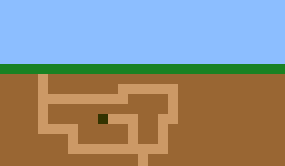
\includegraphics[width=\textwidth]{../img/blockmole-sky-grass.png}
%  \caption{En lundensisk blockmullvad fångad på bild under aktivt grävanade.}
  \label{lab:blockmole:fig:mole}
\end{figure}
\end{minipage}%
%
\hfill\begin{minipage}{0.45\textwidth}
\noindent\textbf{Blockmullvad} (\textit{Talpa laterculus}) är ett fantasidjur i familjen mullvadsdjur.
Den är känd för sitt karaktäristiska kvadratiska utseende.
Den lever mest ensam i sina underjordiska gångar som, till skillnad från den verkliga mullvadens (\emph{Talpa europaea}) gångar, har helt raka väggar.
\end{minipage}



\subsection{Obligatoriska uppgifter}


\Task \emph{Skapa katalog och kodfil.}
Du ska, steg för steg, skapa ett program som låter användaren interagera med en levande blockmullvad. Använd en editor, t.ex. \texttt{atom}, kompilera ditt program i terminalen med \texttt{scalac} och kör med \texttt{scala}.

\Subtask
Skapa en ny fil med namnet \texttt{blockmole.scala} i en ny katalog i din hemkatalog, till exempel \texttt{\textasciitilde/pgk/w04/lab/blockmole.scala}, där \texttt{\textasciitilde} är din hemkatalog.
\begin{REPLnonum}
> mkdir -p ~/pgk/w04/lab
> atom ~/pgk/w04/lab/blockmole.scala
\end{REPLnonum}


\Subtask
Navigera till din nya katalog med \texttt{cd}-kommandot \Eng{change directory} och kontrollera med \texttt{ls}-kommandot \Eng{list} att din nya fil finns där.
\begin{REPLnonum}
> cd ~/pgk/w04/lab/
> ls
\end{REPLnonum}
Om allt går bra ska \texttt{ls}-kommandot skriva ut \texttt{blockmole.scala}.

\Subtask
Gå tillbaka till din texteditor och gör i början av filen \code{blockmole.scala} en paketdeklaration så att koden ingår i paketet \code{blockmole}.

\Subtask
Deklarera sedan ett singelobjekt med namnet \code{Main} och lägg till en \code{main}-funktion i objektet som skriver ut texten: \texttt{"Keep on digging!"}

\Subtask
Kompilera ditt program. När du rätta eventuella fel, ett i taget, och lyckats kompilera helt utan fel, kontrollera med \texttt{ls}-kommandot att några filer som slutar på \texttt{class} har skapats i subkatalogen \code{blockmole}. \Pen Varför hamnade bytekoden i denna katalog?

\Subtask
Kör kommandot \texttt{scala blockmole.Main} för att exekvera ditt program.
Om allt går bra ska texten du angivit skrivas ut i terminalfönstret.

\vspace{1em}\noindent Nu har du skrivit ett program som skriver ut en uppmaning till en mullvad att fortsätta gräva.
Det programmet är inte så användbart, eftersom mullvadar inte kan inte läsa. Nästa steg är därför att skriva ett grafiskt program.%, snarare än ett textbaserat.






\Task \emph{Skapa en grundstruktur för programmet.}
I mindre program fungerar det bra att samla många funktioner i samma singelobjekt, men i stora program blir det lättare att hitta i koden och förstå vad den gör om man har flera moduler med olika ansvar. Ditt program ska ha följande övergripande struktur:

\begin{Code}
package blockmole

object Colors {
  // Samlar olika färger som behövs i övriga objekt
}

object Graphics {
  // Har ett SimpleWindow och procedurer för blockgrafik
}

object Mole {
  // Representerar en blockmullvad som kan gräva:
  def dig(): Unit = println("Här ska det grävas!")
}

object Main {
  def drawWorld(): Unit = println("Ska rita ut underjorden!")

  def main(args: Array[String]): Unit = {
    drawWorld()
    Mole.dig()
  }
}
\end{Code}

Vi lägger i denna laboration alla moduler i samma fil, men om modulerna blir stora och ska återanvändas av flera olika program är det bra att ha dem i olika filer så att de kan kompileras och testas separat.

\Subtask Skapa programskelettet ovan i filen \code{blockmole.scala} och se till att koden kompilerar utan fel och går att köra med utskrifter som förväntat.

\Subtask I singelobjektet \code{Color} ska vi lägga in färger med hjälp av Java-klassen \code{java.awt.Color}. Eftersom vårt singelobjektnamn''krockar'' med namnet på färgklassen i Java-paketet  så byter vi namn på Java-klassen till \code{Jcolor} i importdeklarationen. Lägg in en importdeklaration med namnbytet direkt efter paketdeklarationen. Vi lägger importen så att den syns i hela paketet eftersom flera objekt behöver tillgång till \code{JColor}. Säkerställ att koden fortfarande kompilerar utan fel.

\Subtask Lägg in nedan färger i objektet \code{Colors}:
\begin{Code}
object Color {
  val black  = new JColor(  0,   0,   0)
  val mole   = new JColor( 51,  51,   0)
  val soil   = new JColor(153, 102,  51)
  val tunnel = new JColor(204, 153, 102)
}
\end{Code}


\Subtask Lägg till nedan tre variabler i singelobjektet \code{Graphics}:

\begin{Code}
val windowSize = (30, 50)  // number of blocks width, height
val blockSize  = 10        // number of pixels per block

val win = new SimpleWindow(???, ???, ???)
\end{Code}

\begin{itemize}%[noitemsep]
  \item Gör så att storleken på \code{win} motsvarar blockstorleken gånger fönsterstorleken.
  \item Ge fönstret en lämplig tiltel, t.ex. \code{"Digging Blockmole"}.
  \item Gör en lokal import-deklaration i \code{Graphics} då det bara är detta objekt som behöver tillgång till \code{SimpleWindow}.
  \item När du kompilerar behöver du se till att \code{cslib} finns tillgänglig på \code{classpath} (se övning \texttt{\ExeWeekFOUR}).
  \item Om du glömt ordningen på parametrarna till klassen \code{SimpleWindow} så kolla i dokumentationen\footnote{\url{http://cs.lth.se/pgk/api/}}. Det går tyvärr inte att använda namngivna argument när man använder Java-klasser.
\end{itemize}

\Subtask Lägg till en enkel utritning genom att i proceduren \code{drawWorld} använda \code{Graphics.win}, för att se så att allt fungerar så här långt, till exempel:
\begin{Code}
  def drawWorld(): Unit = Graphics.win.lineTo(100,100)
\end{Code}
Kompilera och kör och säkerställ att allt fungerar som förväntat.


\Task Nu har du gjort ett grafiskt program, men ännu syns ingen mullvad.
Det är dags att skapa koordinatsystemet i blockmullvadens blockvärld.

\Subtask\Pen
Inför redovisningen: säkerställ att du kan förklara vad \code{x}- och \code{y}-parametrarna i \code{SimpleWindow.lineTo} innebär, genom att med papper och penna rita en enkel skiss av ungefär var positionerna $(0,0)$, $(300, 0)$, $(0, 300)$ och $(300, 300)$ ligger i ett fönster som är 300 bildpunkter \Eng{pixels} brett och 500 bildpunkter högt.

\Subtask
Nu ska du skapa ett nytt koordinatsystem för \code{Graphics} som har \emph{stora} bildpunkter.
Vi kallar \code{Graphics} stora bildpunkter för \emph{block} för att lättare skilja dem från de enpixelstora bildpunkterna i \code{SimpleWindow}.

\begin{framed}
\noindent I block-koordinatsystemet för \code{Graphics} gäller följande:

 Om blockstorleken är $b$, så ligger koordinaten $(x, y)$ i \code{Graphics} på koordinaten $(bx, by)$ i \code{SimpleWindow}.

\end{framed}

\noindent Implementera funktionen \code{block} i modulen \code{Graphics} enligt nedan, så att ett block ritas ut. Parametern \code{point} anger blockkoordinaten och parametern \code{color} anger färgen. Fyll i det som saknas.
\begin{Code}
  def block(point: (Int, Int))(color: JColor = Color.black): Unit = {
    win.setLineColor(color)
    val (left, top)     = (point._1 * blockSize, point._2 * blockSize)
    val (right, bottom) = (left + blockSize - 1, top + blockSize - 1)
    for (row <- top to bottom) {
      ???
    }
  }
\end{Code}
Säkerställ att koden kompilerar utan fel.

\Subtask\Pen
Metoden \code{block} ritar ett antal linjer.
Hur många linjer ritas ut?
I vilken ordning ritas linjerna?
Skriv ner dina svar inför redovisningen.

\Subtask
Anropa funktionen \code{Graphics.block} några gånger i \code{Main.drawWorld} så att några block ritas upp i fönstret när programmet körs. Kompilera och kör ditt program och kontrollera att allt fungerar som det ska.




\Task \emph{Rektangelprocedur.}
Nu ska du skriva en funktion för att rita en rektangel. Rektangeln ska ritas med hjälp av funktionen \code{block}.
Sen ska du rita upp mullvadens underjordiska värld med hjälp av denna funktion.

\Subtask
Lägg till en funktion i objektet \code{Graphics} med namnet \code{rectangle} som tar fem parametrar \code{x}, \code{y}, \code{width} och \code{height} av typen \code{Int} och \code{color} av typen \code{Color}.
Parametrarna \code{x} och \code{y} anger \code{Graphics}-koordinaten för rektangelns övre vänstra hörn och \code{width} och \code{height} anger bredden respektive höjden.
Använd följande \code{for}-satser för att rita ut rektangeln.
\begin{Code}
for (yy <- y until (y + height)) {
	for (xx <- x until (x + width)) {
		block(xx, yy, color)
	}
}
\end{Code}

\Subtask\Pen
I vilken ordning ritas blocken ut?

% \Subtask\Pen (Fråga något om skuggning gällande \code{width} och \code{height}.)

\Subtask
Skriv en funktion i objektet \code{Mole} med namnet \code{drawWorld} som ritar ut mullvadens värld, det vill säga en massa jord där den kan gräva sina tunnlar.
\code{Mole.drawWorld} ska inte ha några parametrar och returtypen ska vara \code{Unit} och den ska anropa \code{Graphics.rectangle} för att rita en rektangel med färgen \code{Colors.soil} som precis täcker fönstret.
Eftersom funktionen har många parametrar som lätt kan blandas ihop ska du använda namngivna argument vid anropet.
(Om du har glömt hur man använder namngivna argument kan du titta på övningarna i kapitel~\ref{exe:W03}.)

\Subtask
Anropa \code{Mole.drawWorld} i \code{Mole.main} och testa så att det fungerar.

\Task
I \code{SimpleWindow} finns funktioner för att känna av tangenttryckningar och musklick.
Du ska använda de funktionerna för att styra en liten blockmullvad.

\Subtask
Importera \code{cslib.window.SimpleWindow} i \code{Graphics} och lägg till denna metod:
\begin{Code}
def waitForKey(): Char = {
  w.waitForEvent()
  while (w.getEventType() != SimpleWindow.KEY_EVENT) w.waitForEvent()
  w.getKey
}
\end{Code}
Det finns olika sorters händelser som ett \code{SimpleWindow} kan reagera på, till exempel tangenttryckningar och musklick.
Funktionen som du precis lagt in väntar på en händelse i ditt \code{SimpleWindow} (\code{w.waitForEvent}) ända tills det kommer en tangenttryckning (\code{KEY_EVENT}).
När det kommit en tangenttryckning anropas \code{w.getKey} för att ta reda på vilken bokstav eller vilket tecken det blev, och det resultatet blir också resultatet av \code{waitForKey}, eftersom det ligger sist i blocket.

\Subtask
Lägg till en funktion i objektet \code{Mole} med namnet \code{dig}, utan parametrar och med returtypen \code{Unit}.
Funktionens kropp ska se ut såhär (fast utan \code{???}):
\begin{Code}
{
  var x = Graphics.width / 2
  var y = Graphics.height / 2
  while (true) {
    Graphics.block(x, y, Colors.mole)
    val key = Graphics.waitForKey()
    if (key == 'w') ???
    else if (key == 'a') ???
    else if (key == 's') ???
    else if (key == 'd') ???
  }
}
\end{Code}
Fyll i alla \code{???} så att \code{'w'} styr mullvaden ett steg uppåt, \code{'a'} ett steg åt vänster, \code{'s'} ett steg nedåt och \code{'d'} ett steg åt höger.

\Subtask
Ändra \code{Mole.main} så att den bara innehåller två anrop: ett till \code{drawWorld} och ett till \code{dig}.
Kompilera och kör ditt program för att se om programmet reagerar på w, a, s och d.

\Subtask
Om programmet fungerar kommer det bli många mullvadar som tillsammans bildar en lång mask, och det är ju lite underligt.
Lägg till ett anrop i \code{Mole.dig} som ritar ut en bit tunnel på position $(x, y)$ efter anropet till \code{Graphics.waitForKey} men innan \code{if}-satserna.
Kompilera och kör ditt program för att gräva tunnlar med din blockmullvad.

\subsection{Kontrollfrågor}\Checkpoint

\noindent Repetera teorin för denna vecka och var beredd på att kunna svara på dessa frågor när det blir din tur att redovisa vad du gjort under laborationen:

\begin{enumerate}
\item Till vad används \emph{classpath}?
\item Vad är en \code{jar}-fil?
\item Vad innebär punktnotation?
\item Ge exempel på användning av \code{import} och förklara vad som händer.
\item Vad är fördelen med skuggning och lokala namn?
\item Vi använde flera singelobjekt som olika s.k. \code{moduler} i denna laboration. Vad är fördelen med att att dela upp koden i moduler?
\end{enumerate}

\clearpage

\subsection{Frivilliga extrauppgifter}

\Task
Mullvaden kan för tillfället gräva sig utanför fönstret.
Lägg till några \code{if}-satser i början av \code{while}-satsen som upptäcker om \code{x} eller \code{y} ligger utanför fönstrets kant och flyttar i så fall tillbaka mullvaden precis innanför kanten.

\Task
Mullvadar är inte så intresserade av livet ovanför jord, men det kan vara trevligt att se hur långt ner mullvaden grävt sig.
Lägg till en himmelsfärg och en gräsfärg i objektet \code{Colors} och rita ut himmel och gräs i \code{Mole.drawWorld}.
Justera också det du gjorde i föregående uppgift, så mullvaden håller sig under jord.
(\emph{Tips:} Den andra parametern till \code{Color} reglerar mängden grönt och den tredje parametern reglerar mängden blått.)

\Task
Ändra så att mullvaden kan springa uppe på gräset också, men se till så att ingen tunnel ritas ut där.

\Task
Skriv om loopen i \code{Graphics.waitForKey} så att den använder \code{do while} i stället. Vilken variant tycker du är lättast att förstå?

\Task
Låt mullvaden fortsätta gräva även om man inte trycker ned någon tangent. Tangenttryckning ska ändra riktningen.

\Subtask
Skapa en ny metod \code{Graphics.waitForKeyNonBlocking} som möjliggör tangentbordsavläsning som ej blockerar exekveringen enligt nedan:

\begin{Code}
  def waitForKeyNonBlocking(): Char  = {
    w.waitForEvent(10) //wait max 10 milliseconds
    if (w.getEventType() == SimpleWindow.KEY_EVENT) w.getKey else 0
  }
\end{Code}

\Subtask
Lägg till en ny metod \code{Graphics.delay} som ska göra det möjligt att hindra blockmullvaden från att springa alltför fort:
\begin{Code}
def delay(millis: Int): Unit = SimpleWindow.delay(millis)
\end{Code}


\Subtask
Skapa en ny metod \code{Graphics.keepOnDigging} som från början är en kopia av metoden \code{dig}. Gör följande tillägg/ändringar:
\begin{enumerate}[nolistsep,noitemsep]

\item Lägg till två variabler \code{var dx} och \code{var dy} i början, som ska hålla reda på riktningen som sköldpaddan gräver. Initialisera dem till \code{0} respektive {1}.

\item Lägg in en fördröjning på 200 millisekunder i den oändliga loopen.

\item Kolla efter knapptryckning enligt nedan kodskellett. Fyll i de saknade delarna så att blockmullvaden rör sig ett steg i rätt riktning i varje looprunda.
\begin{Code}
      val key = Graphics.waitForKeyNonBlocking()
      if      (key == 'w') { dy = -1; dx = 0 }
      else if (key == 'a') { ??? }
      else if (key == 's') { ??? }
      else if (key == 'd') { ??? }
      y += ???
      x += ???
\end{Code}

\item Anpassa fördröjningen efter din förmåga att hinna styra blockmullvaden.

\end{enumerate}


%!TEX encoding = UTF-8 Unicode

%!TEX root = ../compendium1.tex

%!TEX encoding = UTF-8 Unicode
\chapter{Klasser}\label{chapter:W05}
Begrepp som ingår i denna veckas studier:
\begin{itemize}[noitemsep,label={$\square$},leftmargin=*]
\item objektorientering
\item klass
\item instans
\item Point
\item Square
\item Complex
\item Any
\item isInstanceOf
\item toString
\item new
\item null
\item this
\item accessregler
\item private
\item private[this]
\item klassparameter
\item primär konstruktor
\item fabriksmetod
\item alternativ konstruktor
\item förändringsbar
\item oföränderlig
\item case-klass
\item kompanjonsobjekt
\item referenslikhet
\item innehållslikhet
\item eq
\item ==\end{itemize}

\clearpage
%!TEX encoding = UTF-8 Unicode
%!TEX root = ../lect-w05.tex

%%%

%TODO:
%  \begin{itemize}
%  \item Bygg upp \code{case class Complex(re: Double, im: Double)} steg för steg inspirerat av Pins3ed kap 6 i likhet med hur de gör med Rational
%  \item Illustrera följande begrepp: this (behövs i max(that)), method overloading behövs för att plussa med både Complex och Double
%  \item Till fördjupningsövning: dekorera Double med metoderna im och re samt (Double, Double) med metoden ir (för irrational) med implicit klass
%  \item Till extrauppgift: implementera klassen Polar(r, fi) med polära koordinater \url{https://sv.wikipedia.org/wiki/Pol%C3%A4ra_koordinater}
%  \end{itemize}

\Subsection{Vad är en klass?}

\ifkompendium
Begreppet \Emph{klass} är en viktig abstraktionsmekanism inom \Emph{objekt-orienterad programmering} (OOP). Klasser används för att samla funktioner och data. En klass har ett namn och kan ha parametrar. En klass deklareras med nyckelordet \code{class} och är en beskrivning hur en viss typ av objekt ska utformas när de så småningom skapas. Det går att skapa \Alert{många} objekt ur en och samma klass. 
\fi


\begin{Slide}{En metafor för klass: Stämpel}\SlideFontSmall
\begin{multicols}{2}

En klass liknar en \Emph{stämpel}.

\vspace{1em}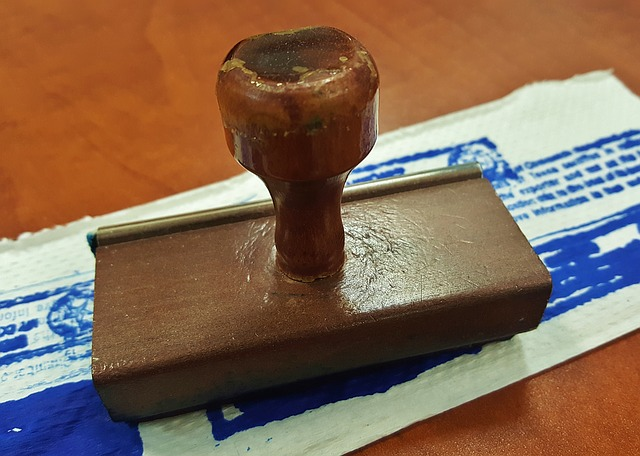
\includegraphics[width=0.5\textwidth]{../img/stamp}

\columnbreak

\pause

\begin{itemize}
\item En stämpel kan \Alert{tillverkas} -- motsvarar \Emph{deklaration} av klassen.
 \item Det händer inget förrän man \Alert{stämplar} -- motsvarar \Emph{instansiering}.
\item Då skapas \Alert{avbildningar} av stämpeln -- motsvarar \Emph{allokering av ett objekt} som är en \Emph{instans} av klassen.
\item Allokering kallas också \Emph{konstruktion} och funktionen/koden som gör själva allokeringen kallas \Emph{konstruktor}.
\end{itemize}

\end{multicols}
\end{Slide}


\begin{Slide}{Vad är en klass?}
\begin{itemize}
\item En klass är en mall \Eng{template} för att skapa objekt.
\item Objekt kan skapas med \code{new Klassnamn}, vilket kallas \Emph{instansiering}. 
\item I Scala 3 är \code{new} valfritt, det räcker med \code{Klassnamn()}. 
\item Ett objekt som skapats med en klassen \code{Klassnamn} som mall kallas för en \Emph{instans} av klassen \code{Klassnamn}.
\item En klass innehåller \Emph{medlemmar} \Eng{members}, som bl.a. kan vara:
  \begin{itemize}
  \item \Emph{attribut}, kallas även fält \Eng{field}: \code{val}, \code{lazy val}, \code{var}
  \item \Emph{metoder}, kallas även operationer: \code{def}
  \end{itemize}
\item Varje instans har sin uppsättning värden på attributen
vilka tillsammans utgör instansens \Emph{tillstånd}.
\end{itemize}

\end{Slide}
  


% \begin{Slide}[t]{Klass och instans}
% \vspace{-0.65em}
% \begin{REPLnonum}
% scala> class C { var attr = 42 }
%
% scala> val objRef1 = new C
% \end{REPLnonum}
% \vspace{3.7em}
% \begin{tikzpicture}[font=\SlideFontSmall\sffamily]
% \matrix [matrix of nodes, row sep=0, column 2/.style={nodes={rectangle,draw,minimum width=0.8cm}}] (mat)
% {
% \texttt{objRef1}   &  \makebox(10,10){ }\\
% };
%
% \node[cloud, cloud puffs=15.0, cloud ignores aspect, minimum width=2cm, minimum height=2cm,
%  align=center, draw] (instance1) at (3.8cm, 0.0cm) {
%  \begin{tabular}{r l}
%  \texttt{attr} & \fbox{42} \\
%  \end{tabular}
%  };
%
%
% \filldraw[black] ($ (mat-1-2) + (0.0cm,0.0cm) $) circle (3pt) node[] (ref1)  {};
% \draw [arrow, line width=0.7mm] (ref1) -- (instance1);
% \end{tikzpicture}
% \end{Slide}
%
%
%
% \begin{Slide}[t]{Klass och instans}
% \vspace{-0.5em}
% \begin{REPLnonum}
% scala> class C { var attr = 42 }
%
% scala> val objRef1 = new C
%
% scala> val objRef2 = new C
% \end{REPLnonum}
% \vspace{2em}
% \begin{tikzpicture}[font=\SlideFontSmall\sffamily]
% \matrix [matrix of nodes, row sep=0, column 2/.style={nodes={rectangle,draw,minimum width=0.8cm}}] (mat)
% {
% \texttt{objRef1}   &  \makebox(10,10){ }\\
% \texttt{objRef2}   &  \makebox(10,10){ }\\
% };
%
% \node[cloud, cloud puffs=15.0, cloud ignores aspect, minimum width=2cm, minimum height=2cm,
%  align=center, draw] (instance1) at (3.8cm, 0.35cm) {
%  \begin{tabular}{r l}
%  \texttt{attr} & \fbox{42} \\
%  \end{tabular}
%  };
%
% \node[cloud, cloud puffs=15.0, cloud ignores aspect, minimum width=2cm, minimum height=2cm,
%  align=center, draw] (instance2) at (5.8cm, -1.5cm) {
%  \begin{tabular}{r l}
%  \texttt{attr} & \fbox{42} \\
%  \end{tabular}
%  };
%
% \filldraw[black] ($ (mat-1-2) + (0.0cm,0.0cm) $) circle (3pt) node[] (ref1)  {};
% \draw [arrow, line width=0.7mm] (ref1) -- (instance1);
%
% \filldraw[black] ($ (mat-2-2) + (0.0cm,0.0cm) $) circle (3pt) node[] (ref2)  {};
% \draw [arrow, line width=0.7mm] (ref2) -- (instance2);
% \end{tikzpicture}
% \end{Slide}
%
%
%
% \begin{Slide}[t]{Klass och instans}
% \vspace{-0.5em}
% \begin{REPLnonum}
% scala> class C { var attr = 42 }
%
% scala> val objRef1 = new C
%
% scala> val objRef2 = new C
%
% scala> objRef2.attr = 43
% \end{REPLnonum}
% \begin{tikzpicture}[font=\SlideFontSmall\sffamily]
% \matrix [matrix of nodes, row sep=0, column 2/.style={nodes={rectangle,draw,minimum width=0.8cm}}] (mat)
% {
% \texttt{objRef1}   &  \makebox(10,10){ }\\
% \texttt{objRef2}   &  \makebox(10,10){ }\\
% };
%
% \node[cloud, cloud puffs=15.0, cloud ignores aspect, minimum width=2cm, minimum height=2cm,
%  align=center, draw] (instance1) at (3.8cm, 0.35cm) {
%  \begin{tabular}{r l}
%  \texttt{attr} & \fbox{42} \\
%  \end{tabular}
%  };
%
% \node[cloud, cloud puffs=15.0, cloud ignores aspect, minimum width=2cm, minimum height=2cm,
%  align=center, draw] (instance2) at (5.8cm, -1.5cm) {
%  \begin{tabular}{r l}
%  \texttt{attr} & \fbox{43} \\
%  \end{tabular}
%  };
%
%
% \filldraw[black] ($ (mat-1-2) + (0.0cm,0.0cm) $) circle (3pt) node[] (ref1)  {};
% \draw [arrow, line width=0.7mm] (ref1) -- (instance1);
%
% \filldraw[black] ($ (mat-2-2) + (0.0cm,0.0cm) $) circle (3pt) node[] (ref2)  {};
% \draw [arrow, line width=0.7mm] (ref2) -- (instance2);
% \end{tikzpicture}
% \end{Slide}



\begin{Slide}{Singelobjekt jämfört med klass}\SlideFontSmall
Vi har tidigare deklarerat \Emph{singelobjekt} som bara finns i \Alert{en} enda upplaga:
\begin{REPLnonum}
scala> object Björn { var ålder = 53; val längd = 178 }
\end{REPLnonum}

Med en \Emph{klass} kan man skapa \Alert{godtyckligt många} \Emph{instanser av klassen} med hjälp av nyckelordet \code{new} följt av klassens namn:

\begin{REPLnonum}
scala> class Person { var ålder = 0; var längd = 0 }

scala> val björn = new Person   // allokera plats i minnet
björn: Person = Person@7ae75ba6  // unikt id för instansen
\end{REPLnonum}
\begin{tikzpicture}[font=\small\sffamily]
\matrix [matrix of nodes, row sep=0, column 2/.style={nodes={rectangle,draw,minimum width=0.8cm}}] (mat)
{
\texttt{björn}   &  \makebox(10,10){ }\\
};
\node[cloud, cloud puffs=12.0, cloud ignores aspect, minimum width=2cm, minimum height=3.8cm,
 align=center, scale=0.8, draw] (x) at (3.8cm, -1.0cm) {
 \begin{tabular}{r l}
 \multicolumn{2}{c}{\ttfamily\itshape Person@7ae75ba6}\\ \\
 \texttt{ålder} & \fbox{~0~} \\
 \texttt{längd} & \fbox{~0~}\\
 \end{tabular}
 };
\filldraw[black] (0.6cm,0.0cm) circle (3pt) node[] (ref) {};
\draw [arrow, line width=0.7mm] (ref) -- (x);
\end{tikzpicture}
\end{Slide}


\begin{Slide}{Förändring av objektets tillstånd}
\begin{REPLnonum}
scala> björn.ålder = 53

scala> björn.längd = 178
björn: Person = Person@7ae75ba6
\end{REPLnonum}

\begin{tikzpicture}[font=\large\sffamily]
\matrix [matrix of nodes, row sep=0, column 2/.style={nodes={rectangle,draw,minimum width=0.8cm}}] (mat)
{
\texttt{björn}   &  \makebox(10,10){ }\\
};
\node[cloud, cloud puffs=13.0, cloud ignores aspect, minimum width=2cm, minimum height=3.8cm,
 align=center, draw] (x) at (5.8cm, -1.2cm) {
 \begin{tabular}{r l}
 \multicolumn{2}{c}{\ttfamily\itshape Person@7ae75ba6}\\ \\
 \texttt{ålder} & \fbox{~53~} \\
 \texttt{längd} & \fbox{~178~}\\
 \end{tabular}
 };
\filldraw[black] (0.75cm,0.0cm) circle (3pt) node[] (ref) {};
\draw [arrow, line width=0.7mm] (ref) -- (x);
\end{tikzpicture}
%{\SlideFontTiny{\ttfamily\itshape Person@7ae75ba6} är en unik idenfierare för instansen, så att JVM hittar den i heapen.}
\end{Slide}


\begin{Slide}{Bättre att initialisera med hjälp av klassparametrar}
\begin{REPLnonum}
scala> class Person(var ålder: Int, var längd: Int)

scala> val sandra = new Person(42, 166)
sandra: Person = Person@7878bbdb
\end{REPLnonum}

\begin{tikzpicture}[font=\large\sffamily]
\matrix [matrix of nodes, row sep=0, column 2/.style={nodes={rectangle,draw,minimum width=0.8cm}}] (mat)
{
\texttt{sandra}   &  \makebox(10,10){ }\\
};
\node[cloud, cloud puffs=13.0, cloud ignores aspect, minimum width=2cm, minimum height=3.8cm,
 align=center, draw] (x) at (5.8cm, -1.2cm) {
 \begin{tabular}{r l}
 \multicolumn{2}{c}{\ttfamily\itshape Person@7878bbdb}\\ \\
 \texttt{ålder} & \fbox{~42~} \\
 \texttt{längd} & \fbox{~166~}\\
 \end{tabular}
 };
\filldraw[black] (0.75cm,0.0cm) circle (3pt) node[] (ref) {};
\draw [arrow, line width=0.7mm] (ref) -- (x);
\end{tikzpicture}
%{\SlideFontTiny{\ttfamily\itshape Person@7ae75ba6} är en unik idenfierare för instansen, så att JVM hittar den i heapen.}
\end{Slide}


\begin{Slide}{Klassdeklarationer och instansiering}\SlideFontSmall
\setlength{\leftmargini}{0pt}
\begin{itemize}
\item Syntax för deklaration av klass: \\ \vspace{0.5em}{\SlideFontSize{13}{16}\code|class Klassnamn(parametrar){ medlemmar }|}\vspace{0.5em}
\item Exempel: \Emph{deklaration}
\begin{Code}
class Klassnamn(val attribut1: Int, attribut2: String){
  val attribut3: Double = 42.0              //publikt oföränderligt attribut
  private var attribut4: Boolean = false    //privat medlem syns inte utåt
  def metod(parameter: Int) = parameter + 1 //funktion i klass kallas metod
  lazy val attr5 = Vector.fill(100000)(42.0)     //fördröjd initialisering
}
\end{Code}

\item Parametrar initialiseras med de argument som ges vid \code{new}.
\item Exempel: \Emph{instansiering} med argument för initialisering av klassparametrar
\begin{Code}
val instansReferens = new Klassnamn(42, "hej")  // new är valfritt här 
\end{Code}

\item Parametrar som inte föregås av modifierare (t.ex. private val, val, var) blir \Emph{attribut} som är \code{ private[this] val } och bara är synliga i \Alert{denna} instans.
\item Attribut i klasskroppen är \Emph{publika} (alltså synliga utåt) om inte \code{private} anges.
\end{itemize}
\end{Slide}




\begin{Slide}{Övning: en klass som representerar en person}
\begin{enumerate}
  \item Deklarera en klass \code{Person} med dessa publika attribut:
  \begin{itemize}
    \item oföränderligt förnamn
    \item oföränderligt efternamn
    \item förändringsbar ålder med defaultargument \code{0}
  \end{itemize}
  \item lägg till en metod i klasskroppen med explicit returtyp som ger en 2-tupel med förnamn och efternamn
  \item skriv en deklaration som deklarerar en variabel \code{p} som initialiseras med värdet av ett uttryck som instansierar klassen \code{Person} med ditt namn och din ålder som nyfödd.
  \item skriv en sats som skriver ut ditt förnamn genom att referera attribut med punktnotation
  \item skriv en tilldelningssats som ändrar tillståndet för den instans som referensen \code{p} refererar till så att åldersattributets värde blir din nuvarande ålder
\end{enumerate}
\end{Slide}



\begin{Slide}{Lösning: klassen Person}
\begin{Code}[basicstyle=\SlideFontSize{6.9}{9}\ttfamily]
class Person(val givenName: String, val familyName: String, var age: Int = 0){
  def name: (String, String) = (givenName, familyName)
}
\end{Code}
\begin{REPLnonum}[basicstyle=\SlideFontSize{7}{9}\ttfamily\color{white}]
val p = Person("Björn", "Regnell")
println(p.name._1)
p.age = 50
\end{REPLnonum}
\end{Slide}


\begin{Slide}{Instansprivata klassparametrar}\SlideFontSmall
\setlength{\leftmargini}{0pt}

\begin{itemize}
\item Parametrar som inte föregås av modifierare (t.ex. private val, val, var) blir \Emph{attribut} som är \code{ private[this] val } och bara är synliga i \Alert{denna} instans.
\item Exempel på konsekvensen av \code{private[this]}:
\begin{REPL}[basicstyle=\SlideFontSize{6.7}{9}\ttfamily\color{white}]
scala> class C(a: Int){ def add(other: C): Int = a + other.a }
error: value a is not a member of C

// betyder samma sak som:

scala> class C(private[this] val a: Int){ def add(other: C): Int = a + other.a }
error: value a is not a member of C
\end{REPL}
\item Men detta fungerar fint:
\begin{REPL}
scala> class D(val a: Int){ def add(other: D): Int = a + other.a }

scala> D(42).add(D(43))
res0: Int = 85
\end{REPL}
...eftersom modifieraren \code{val} framför klassparameter ger publik synlighet.
\item Vad händer om du skriver \code{private val} framför klassparametern \code{a} ovan?
\end{itemize}
\end{Slide}


\begin{Slide}{\texttt{private} jämfört med \texttt{private[this]}}\SlideFontSmall
\code{private[this]} är \Alert{ännu} mer privat än \code{private}
\begin{Code}
class Hemlis(private val hemlis: Int) {
  def ärSammaSom(annan: Hemlis) = hemlis == annan.hemlis   // Funkar!
}

class Hemligare(private[this] val hemlis: Int) {
  def ärSammaSom(annan: Hemligare) = hemlis == annan.hemlis //KOMPILERINGSFEL
}
\end{Code}
\pause Vad händer om man inte skriver ens \code{val}? \pause Olika för klass och s.k. case-klass:
\begin{Code}
class Hemligare(hemlis: Int) { // motsvarar private[this] val
  def ärSammaSom(annan: Hemligare) = hemlis == annan.hemlis //KOMPILERINGSFEL
}

case class InteHemlig(seMenInteRöra: Int) { // blir automatiskt val
  def ärSammaSom(annan: InteHemlig): Boolean =
    seMenInteRöra == annan.seMenInteRöra
}

\end{Code}
{\SlideFontTiny Vi ska lära mer om det godis man får på köpet med \code{case}-klasser om ett litet tag.}
\end{Slide}



%%%%%%%%%%%% ÄR EXEMPEL KOMPLEXA TAL ÄR FÖR SVÅR MATEMATIK för lp1???? %%%%%%%%%
%% Nej komplexa tal som vektor med polära koordinater ingår i matte 4 som är krav för LTH: %%%


\begin{Slide}{Övning: Klassen Complex i Scala}\SlideFontSmall
Implementera klassen \code{Complex} nedan som representerar komplexa tal:
\begin{Code}
  class Complex(val re: Double, val im: Double):
    def r  = ???  // absolutbeloppet
    def fi = ???  // vinkeln i radianer
    def +(other: Complex): Complex = ???  // resultatet av addition
    var imSymbol = 'i'  // symbol för imaginärdel, används i toString
    override def toString = ???  // en strängrepresentation av talet
\end{Code}

\begin{minipage}{0.3\textwidth}
  Exempel: \\$z = 3 + 4i$
\end{minipage}
\begin{minipage}{0.5\textwidth}
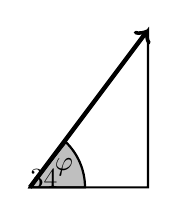
\begin{tikzpicture}[thick]
\coordinate (O) at (0,0);
\coordinate (A) at (1.5,0);
\coordinate (B) at (1.5,2.0);

%\tkzMarkAngle[fill=orange,size=0.5cm, opacity=.4](A,O,B) 
%\tkzLabelAngle[pos=0.8](A,O,B){\texttt{$\varphi$}}
 %%% AAAARGH ovan slutade funka så gjorde nedan HACK i stället
\draw[fill=lightgray, thick] (0,0) -- (0:0.7cm) arc (0:46:0.8cm) node at (30:0.5cm) {$\varphi$} -- cycle;
%\draw[fill=lightgray, thick] (0,0) -- (0:0.7cm) arc (0:45:0.8cm) node at (30:0.5cm) {$\varphi$} -- cycle;
%https://tex.stackexchange.com/questions/96459/automatically-draw-and-labels-angles-of-a-triangle-in-tikz

\draw (O)--(A)--(B)--cycle;
\draw [->, ultra thick] (O)--(B);

\tkzLabelSegment[below=5pt](O,A){\textit{real-delen} är $3$}
\tkzLabelSegment[above left=5pt](O,B){\textit{r}}
\tkzLabelSegment[right=5pt](A,B){\textit{imaginär-delen} är $4$}


\end{tikzpicture}
\end{minipage}

\end{Slide}


\begin{Slide}{Exempel: Klassen Complex i Scala}\SlideFontSmall
\scalainputlisting[basicstyle=\ttfamily\SlideFontSize{7}{9}]{../compendium/examples/complex1.scala}
%Klassparametrarna är parametrar till den s.k. \Emph{primärkonstruktorn}.
\begin{REPL}
scala> val z = new Complex(3, 4)  // konstruktion av instans av Complex
z: Complex = 3.0 + 4.0i

scala> val polärForm = (c1.r, c1.fi)
polärForm: (Double, Double) = (5.0,0.6435011087932844)

scala> val z2 = new Complex(1, 2)
z2: Complex = 1.0 + 2.0i

scala> z1 + z2
res0: Complex = 4.0 + 6.0i
\end{REPL}
\end{Slide}



\begin{Slide}{Exempel: Principen om enhetlig access}\SlideFontSmall
\scalainputlisting[basicstyle=\ttfamily\SlideFontSize{7}{9}]{../compendium/examples/complex2.scala}
\pause
\begin{itemize}
\item Efter som attributen \code{re} och \code{im} är oföränderliga, kan vi lika gärna ändra i klass-implementationen och göra om metoderna \code{r} och \code{fi} till \code{val}-variabler utan att klientkoden påverkas.

\item Då anropas \code{math.hypot} och \code{math.atan2} bara en gång vid initialisering (och inte varje gång som med \code{def}).

\item Vi skulle även kunna använda \code{lazy val} och då bara räkna ut \code{r} och \code{fi} om och när de verkligen refereras av klientkoden, annars inte.

\item Eftersom klientkoden inte ser skillnad på metoder och variabler, kallas detta \Emph{principen om enhetlig access}. (Många andra språk har \Alert{inte} denna möjlighet, tex Java där metoder \emph{måste} ha parenteser.)
\end{itemize}
\end{Slide}



\Subsection{Olika sätt att skapa instanser}

\begin{Slide}{Instansiering med direkt användning av \texttt{new}}

Instansiering genom \Emph{direkt användning} av \code{new}\\
{\SlideFontSmall (här första varianten av Complex med \code{r} och \code{fi} som metoder)}
\begin{REPLnonum}
scala> val c1 = new Complex(3, 4)
\end{REPLnonum}
\begin{tikzpicture}[font=\SlideFontSmall\sffamily]
\matrix [matrix of nodes, row sep=0, column 2/.style={nodes={rectangle,draw,minimum width=0.8cm}}] (mat)
{
\texttt{c1}   &  \makebox(10,10){ }\\
};

\node[cloud, cloud puffs=15.0, cloud ignores aspect, minimum width=2cm, minimum height=3.8cm,
 align=center, draw] (instance1) at (5.8cm, -1.5cm) {
 \begin{tabular}{r l l}
 \texttt{re:} & \texttt{Double} & \fbox{3.0} \\
 \texttt{im:} & \texttt{Double} & \fbox{4.0}\\
 \texttt{imSymbol:} & \texttt{Char} & \fbox{i}\\
 \end{tabular}
 };

\filldraw[black] ($ (mat-1-2) + (0.0cm,0.0cm) $) circle (3pt) node[] (ref1)  {};

\draw [arrow, line width=0.7mm] (ref1) -- (instance1);
\end{tikzpicture}
\pause
Ofta vill man göra \Alert{indirekt} instansiering så att vi senare har friheten att ändra hur instansiering sker.
\end{Slide}



\begin{Slide}{Indirekt instansiering med fabriksmetoder}\SlideFontSmall
En \Emph{fabriksmetod} är en metod som används för att instansiera objekt.
\begin{Code}[basicstyle=\SlideFontSize{8}{12}\ttfamily\selectfont]
object MyFactory {
  def createComplex(re: Double, im: Double) = new Complex(re, im)
  def createReal(re: Double)                = new Complex(re, 0)
  def createImaginary(im: Double)           = new Complex(0, im)
}
\end{Code}
\pause
Instansiera \Alert{inte direkt}, utan \Emph{indirekt} genom användning av \Emph{fabriksmetoder}:
\begin{REPL}
scala> import MyFactory._

scala> createComplex(3, 4)
res0: Complex = 3.0 + 4.0i

scala> createReal(42)
res1: Complex = 42.0 + 0.0i

scala> createImaginary(-1)
res2: Complex = 0.0 + -1.0i
\end{REPL}
\end{Slide}



\begin{Slide}{Hur förhindra direkt instansiering?}
Om vi vill \Emph{förhindra direkt instansiering} kan vi göra primärkonstruktorn \Alert{privat}:
\scalainputlisting[basicstyle=\ttfamily\SlideFontSize{7}{9}]{../compendium/examples/complex3.scala}
MEN... då går det ju \Alert{inte} längre att instansiera något alls!  \code{   :(}
\begin{REPLnonum}
scala> new Complex(3,4)
error:
 constructor Complex in class Complex cannot be accessed
\end{REPLnonum}
\end{Slide}



\begin{Slide}{Kompanjonsobjekt med indirekt instansiering}\SlideFontSmall
\setlength{\leftmargini}{0pt}
\begin{itemize}
\item Ett \Emph{kompanjonsobjekt} \Eng{companion object} är ett singelobjekt som ligger i \Alert{samma kodfil} som en klass, och som har \Alert{samma namn} som klassen.

\item Medlemmar i ett kompanjonsobjekt \Alert{får accessa privata} medlemmar i kompanjonsklassen (och vice versa) och kompanjonsobjektet får därför accessa privat konstruktor och kan göra \code{new}.
\scalainputlisting[basicstyle=\ttfamily\SlideFontSize{7}{9}]{../compendium/examples/complex4.scala}

\item Fabriksmetoder i kompanjonsobjektet ovan och privat konstruktor gör att vi \Alert{enbart} tillåter \Emph{indirekt instansiering}.
\end{itemize}
\end{Slide}

\begin{Slide}{Användning av kompanjonsobjekt med fabriksmetoder}
Nu kan vi \Alert{bara} instansiera \Emph{indirekt}!  \code{   :)}
\begin{REPLnonum}
scala> Complex.real(42.0)
res0: Complex = 42.0 + 0.0i

scala> Complex.imag(-1)
res1: Complex = 0.0 + -1.0i

scala> Complex.apply(3,4)
res2: Complex = 3.0 + 4.0i

scala> Complex(3,4)
res3: Complex = 3.0 + 4.0i

scala> new Complex(3, 4)
error:
     constructor Complex in class Complex cannot be accessed
\end{REPLnonum}
\end{Slide}


\begin{Slide}{Alternativa direktinstansieringar med default-argument}\SlideFontSmall
Med \Emph{default-argument} kan vi erbjuda \Emph{alternativa} sätt att direktinstansiera.
\scalainputlisting[basicstyle=\ttfamily\SlideFontSize{7}{9}]{../compendium/examples/complex5.scala}
\begin{REPL}
scala> new Complex()
res0: Complex = 0.0 + 0.0i

scala> new Complex(re = 42)  //anrop med namngivet argument
res1: Complex = 42.0 + 0.0i

scala> new Complex(im = -1)
res2: Complex = 0.0 + -1.0i

scala> new Complex(1)
res3: Complex = 1.0 + 0.0i
\end{REPL}
\end{Slide} 

\begin{Slide}{Alternativa sätt att instansiera med fabriksmetod}
Vi kan också erbjuda \Emph{alternativa} sätt att instansiera \Emph{indirekt} med fabriksmetoden \code{apply} i ett kompanjonsobjekt genom default-argument:
\scalainputlisting[basicstyle=\ttfamily\SlideFontSize{7}{9}]{../compendium/examples/complex6.scala}

\end{Slide}

\begin{Slide}{Medlemmar som bara behövs i en enda upplaga}
Attributet \code{imSymbol} passar bättre att ha i \Emph{kompanjonsobjektet}, eftersom det räcker att ha \Alert{en enda upplaga}, som kan vara gemensam för alla objekt:
\scalainputlisting[basicstyle=\ttfamily\SlideFontSize{7}{9}]{../compendium/examples/complex7.scala}

\end{Slide}



\begin{Slide}{Medlemmar i singelobjekt är statiskt allokerade}\SlideFontTiny

Minnesplatsen för \Emph{attribut i singelobjekt} allokeras automatiskt en gång för alla, och kallas därför \Emph{statiskt} allokerad. Singelobjektets namn \code{Complex} utgör en statisk referens till den enda instansen och är av typen \texttt{Complex.type}.

\begin{tikzpicture}[font=\SlideFontSmall\sffamily]
\matrix [matrix of nodes, row sep=0, column 2/.style={nodes={rectangle,draw,minimum width=0.8cm}}] (mat)
{
\texttt{Complex}   &  \makebox(10,10){ }\\
};

\node[cloud, cloud puffs=15.0, cloud ignores aspect, minimum width=1cm, minimum height=2cm,
 align=center, draw] (instance1) at (5.8cm, 0.0cm) {
 \begin{tabular}{r l l}
 \texttt{imSymbol:} & \texttt{Char} & \fbox{i}\\
 \end{tabular}
 };

\filldraw[black] ($ (mat-1-2) + (0.0cm,0.0cm) $) circle (3pt) node[] (ref1)  {};

\draw [arrow, line width=0.7mm] (ref1) -- (instance1);
\end{tikzpicture}

Nu bereder vi inte plats för \code{imSymbol} i varenda \Emph{dynamiskt} allokerade instans:
\begin{REPLnonum}
scala> val c1 = Complex(3, 4)
\end{REPLnonum}

\begin{tikzpicture}[font=\SlideFontSmall\sffamily]
\matrix [matrix of nodes, row sep=0, column 2/.style={nodes={rectangle,draw,minimum width=0.8cm}}] (mat)
{
\texttt{c1}   &  \makebox(10,10){ }\\
};

\node[cloud, cloud puffs=15.0, cloud ignores aspect, minimum width=2cm, minimum height=2cm,
 align=center, draw] (instance1) at (5.8cm, -0.0cm) {
 \begin{tabular}{r l l}
 \texttt{re:} & \texttt{Double} & \fbox{3.0} \\
 \texttt{im:} & \texttt{Double} & \fbox{4.0}\\
 \end{tabular}
 };

\filldraw[black] ($ (mat-1-2) + (0.0cm,0.0cm) $) circle (3pt) node[] (ref1)  {};

\draw [arrow, line width=0.7mm] (ref1) -- (instance1);
\end{tikzpicture}


\end{Slide}




\begin{Slide}{Attribut i kompanjonsobjekt användas för sådant som är gemensamt för alla instanser}

Om vi ändrar på statiska \code{imSymbol} så ändras \code{toString} för \Alert{alla} dynamiskt allokerade instanser.
\begin{REPLnonum}
scala> val c1 = Complex(3, 4)
c1: Complex = 3.0 + 4.0i

scala> Complex.imSymbol = 'j'
Complex.imSymbol: Char = j

scala> val c2 = Complex(5, 6)
c2: Complex = 5.0 + 6.0j

scala> c1
res0: Complex = 3.0 + 4.0j
\end{REPLnonum}
\end{Slide}


\Subsection{Case-klasser och fördelen med oföränderlighet}

\ifkompendium\else
\begin{frame}[plain]
  
\includegraphics[width=1.0\textwidth]{../img/mutant.png}
\end{frame}
\fi

\begin{Slide}{Övning: en läskig mutant}\SlideFontSmall
\begin{enumerate}
\item Skapa en klass med namnet \code{Mutant} som har ett förändringsbart attribut som klassparameter med namnet \code{i} av typen \code{Int} med default-argumentet \code{5}.
\vspace{0.5em}

\item \begin{minipage}{0.5\textwidth}
Deklarera två \code{val}-variabler som kallas \code{fem1} och \code{fem2} och som båda refererar till \Alert{samma} \code{Mutant}-instans.
\end{minipage}
\hfill\begin{minipage}{0.32\textwidth}
\hfill
\includegraphics[width=3.4cm]{../img/mutant.png}

En \code{Mutant}-instans där \code{i} kanske är fem.
\vspace{1em}
\end{minipage}

\item Skriv kod som ändrar tillstånd via den ena mutantreferensen.

\item Syns ändringen via den andra mutantreferensen?
\end{enumerate}
\end{Slide}




\begin{Slide}{Case-klasser}
Case-klasser är ett smidigt sätt att skapa \Emph{oföränderliga} datastrukturer. Med nyckelordet \code{case} framför \code{class} får du mycket ''godis på köpet'':

\begin{itemize}
\item Klassparametrar blir automatiskt publika oföränderliga attribut\footnote{alltså \Alert{inte} \texttt{private[this] val } som i vanliga klasser.} och du slipper alltså skriva \code{val}
\item Du får en automatisk \Emph{toString} med klassens namn och värdet av alla \code{val}-attribut som ges av klassparametrarna och du slipper alltså skriva en egen toString
\item Du får ett automatiskt kompanjonsobjekt med en fabriksmetod \code{apply} för indirekt instansiering där alla klassparametrarnas \code{val}-attribut initialiseras.
\pause
\item ... och mer därtill men mer om det senare...
\end{itemize}
\end{Slide}




\begin{Slide}{Exempel: oföränderliga case-klassen \code{Point}}

\begin{Code}[basicstyle=\SlideFontSize{10}{12}\ttfamily]
case class Point(x: Double, y: Double)
\end{Code}

\begin{REPLnonum}
scala> val p1 = Point(3, 4)
p1: Point = Point(3.0,4.0)

scala> val p2 = p1
p2: Point = Point(3.0,4.0)

scala> p1.x = 42
error: reassignment to val
\end{REPLnonum}
Vi kan utan risk dela med oss av en referens till en oföränderlig klass -- ingen kan ändra dess innehåll. (Jämför läskiga mutanten i tidigare exempel.)

\end{Slide}






\Subsection{Konstruktor}



\begin{Slide}{Vad är en konstruktor?}
\begin{itemize}
\item En \Emph{konstruktor} är den maskinkod som exekveras när klasser instansieras med \code{new}.

\item Konstruktorn skapar ett nytt objekt i minnet vid varje anrop.

\item I Scala \Alert{genererar kompilatorn} en \Emph{primärkonstruktor} åt dig med maskinkod som initialiserar alla attribut baserat på klassparametrarna som du deklarerat.

\pause

%\item I Java och många andra språk får man \Alert{explicit} skriva kod för konstruktorer med speciell syntax och göra alla initialiseringar av attribut själv, och det behövs många olika konstruktorer för att motsvara defaultargument.

\item I Scala \Emph{kan} man också skriva egna alternativa s.k. \Emph{hjälpkonstruktorer}, men det är \Alert{ovanligt}, eftersom man har möjligheten med fabriksmetoder i kompanjonsobjekt och default-argument.
\end{itemize}
\end{Slide}


\begin{Slide}{Hjälpkonstruktorer i Scala (ovanliga)}%\SlideFontSmall
Fördjupning för kännedom:
\begin{itemize}
\item I Scala kan man skapa ett alternativ till primärkonstruktorn, en så kallad \Emph{hjälpkonstruktor} \Eng{auxilliary constructor} genom att deklarera en metod med det speciella namnet \code{this}.


\item Hjälpkonstruktorer \Alert{måste} börja med att anropa en \Alert{annan} konstruktor som står \Alert{före} i koden, till exempel primärkonstruktorn.
\end{itemize}

\begin{Code}
class Point(val x: Int, val y: Int, val z: Int): // primärkonstruktor
  def this(x: Int, y: Int) = this(x, y, 0) // anropa primärkonstruktorn
  def this(x: Int) = this(x, 0) // anropa hjälpkonstruktor
\end{Code}

%{\SlideFontSmall Överlagrade hjälpkonstruktorer i Scala liknar användning av konstruktorer i Java, där man inte har default-argument och apply i kompanjonsobj. etc.}

\end{Slide}

\begin{Slide}{Användning av hjälpkonstruktor}
\begin{REPL}
scala> val p1 = Point(1)
p1: Point = Point@21312342

scala> val p2 = Point(1, 2)
p2: Point = Point@43254325

scala> val p3 = Point(1, 2, 3)
p3: Point = Point@346654
\end{REPL}
\pause
Men man gör \Alert{mycket oftare} så här i Scala:
\begin{Code}[basicstyle=\ttfamily\SlideFontSize{8.5}{12}]
case class Point(x: Int, y: Int = 0, z: Int = 0)
\end{Code}
Använd alltså defaultargument hellre än hjälpkonstruktor.\\
(Eller överlagrad fabriksmetod i kompanjonsobjekt.)
\end{Slide}



% \begin{Slide}{Vad gör skräpsamlaren?}\SlideFontSmall
% \begin{itemize}
% \item Scala och Java är båda programmeringsspråk som förutsätter en körmiljö med \Alert{automatisk}  \Emph{skräpsamling} \Eng{garbage collection}.
%
% \item \Emph{Skräpsamlaren} \Eng{the garbage collector} är ett program som automatiskt körs i bakgrunden då och då och \Emph{städar minnet} genom att frigöra den plats som upptas av \Alert{objekt som inte längre används}.
%
% \item JVM:en bestämmer själv när skräpsamlaren ska jobba och programmeraren har ingen kontroll över detta.
%
% \item Den stora \Emph{fördelen} med automatisk skärpsamling är att man slipper bry sig om det svåra och felbenägna arbetet att \Alert{avallokera} minne.
%
% \item \Alert{Nackdelen} är att man inte kan styra exakt hur och när skräpsamlingen ska ske och man kan därmed inte bestämma när processorn ska belastas med minneshanteringen. Detta är normalt inget problem, utom i vissa tidskritiska realtidssystem med hårda minnesbegränsningar och svarstidskrav.
%
% \item I språk utan automatisk skräpsamling, t.ex. C++, måste man ta hand om destruktion av objekt och skriva egna s.k. \Emph{destruktorer}.
% \end{itemize}
% \end{Slide}


\Subsection{Referens saknas: \texttt{null}}

\begin{Slide}{Referens saknas: \texttt{null}}
\begin{itemize}
\item I Java och många andra språk använder man ofta literalen \code{null} för att representera att ett \Alert{värde saknas}.

\item En referens som är \code{null} refererar inte till någon instans.

\item Om du försöker referera till instansmedlemmar med punktnotation genom en referens som är \code{null} kastas ett \Alert{undantag} \code{NullPointerException}.

\item Oförsiktig användning av \code{null} är en vanlig källa till \Alert{buggar}, som kan vara svåra att hitta och fixa.

\end{itemize}
\end{Slide}


\begin{Slide}{Exempel: \texttt{null}}
\begin{REPL}
scala> class Gurka(val vikt: Int)

scala> var g: Gurka = null        // ingen instans allokerad än
val g: Gurka = null

scala> g.vikt
java.lang.NullPointerException

scala> g = Gurka(42)          // instansen allokeras
val g: Gurka = Gurka@1ec7d8b3

scala> g.vikt
val res0: Int = 42

scala> g = null         // instansen kommer att destrueras av skräpsamlaren
\end{REPL}

\begin{itemize} \SlideFontSmall
\item Scala har \code{null} av kompabilitetsskäl, men det är brukligt att \Alert{endast} använda \code{null} om man anropar Java-kod.

\item Scala erbjuder smidiga \code{Option}, \code{Some} och \code{None} för säker hantering av saknade värden; mer om detta kommande vecka.



\end{itemize}
\end{Slide}


\Subsection{Referensen \texttt{this}}
\begin{Slide}{Referensen \texttt{this}}\SlideFontSmall
\begin{itemize}
\item Nyckelordet \code{this} ger en referens till den aktuella instansen.
\begin{REPLnonum}
scala> class Gurka(var vikt: Int){def jagSjälv = this}

scala> val g = Gurka(42)
val g: Gurka = Gurka@5ae9a829

scala> g.jagSjälv
val res0: Gurka = Gurka@5ae9a829

scala> g.jagSjälv.vikt
val res1: Int = 42

scala> g.jagSjälv.jagSjälv.vikt
val res2: Int = 42
\end{REPLnonum}
\item Referensen \code{this} används ofta för att komma runt ''namnkrockar'' där variabler med samma namn gör så att den ena variabeln inte syns.
\end{itemize}
\end{Slide}



\Subsection{Getters och setters}

\begin{Slide}{Getters och setters}\SlideFontSmall
\begin{itemize}
\item I många språk (t.ex. Java, Python) finns inget motsvarande nyckelord \code{val} som garanterar oföränderliga attributreferenser.
\footnote{Java har visserligen \jcode{final} men det är annorlunda som vi ska se senare.}

\item Därför gör man i dessa språk nästan alltid alla attribut \Alert{privata} för att förhindra att de ändras på ett okontrollerat sätt.

% \item Många språk följer \Alert{inte} principen om enhetlig access: åtkomst av metoder och variabler sker med olika syntax.

\item Därför är det normalt att införa metoder som kallas \Emph{getters} och \Emph{setters}, som används för att \Alert{indirekt} läsa och uppdatera \Emph{attribut}.

\item Dessa metoder känns i många språk igen genom konventionen att de heter något som börjar med \Emph{get} respektive \Emph{set}. (Men \Alert{ej} vanligt i Scala.)

\item Med \Emph{indirekt access} av attribut kan man åstadkomma \Emph{flexibilitet}, så att implementationen kan ändras utan att ändra i klientkoden:
\begin{itemize}\SlideFontSmall
\item[--] man kan t.ex. i efterhand ändra representation av de privata attributen eftersom all access sker genom getters och setters.
\end{itemize}

\item Man kan åstadkomma \Emph{oföränderliga} datastrukturer där attributreferenserna inte förändras efter allokering om klassen \Alert{inte} erbjuder en \Alert{setter} för privata attribut.
\end{itemize}
\end{Slide}



\begin{Slide}{Java-exempel: Klassen JPerson}\SlideFontSmall
\Emph{Indirekt} access av \Alert{privata} attribut:
\vspace{-1em}\begin{multicols}{2}
\javainputlisting[basicstyle=\SlideFontSize{7}{8}\ttfamily\selectfont]{../compendium/examples/JPerson.java}

\columnbreak

\begin{REPLnonum}[basicstyle=\SlideFontSize{7}{9}\ttfamily\color{white}]
$ javac JPerson.java
$ scala
Welcome to Scala 2.11.8 (Java HotSpot(TM) 64-Bit Server VM, Java 1.8.0_66).
Type in expressions for evaluation. Or try :help.

scala> val p = new JPerson("Björn")
p: JPerson = JPerson@7e774085

scala> p.getAge
res0: Int = 0

scala> p.setAge(42)

scala> p.getAge
res1: Int = 42

scala> p.age
error:
value age is not a member of JPerson
\end{REPLnonum}
\end{multicols}
\end{Slide}


\begin{Slide}{Motsvarande JPerson men i Scala}
Så här brukar man åstadkomma ungefär motsvarande i Scala: \\~
\begin{Code}[basicstyle=\SlideFontSize{12}{15}\ttfamily\selectfont]
class Person(val name: String):
  var age = 0
\end{Code}
~\\
Notera att alla attribut här är \Emph{publika}.
\end{Slide}


\begin{Slide}{Förhindra felaktiga attributvärden med setters}\SlideFontSmall
Med hjälp av \Emph{setters} kan vi förhindra \Alert{felaktig} uppdatering av attributvärden, till exempel \Alert{negativ ålder} i klassen \code{JPerson} i Java:
\begin{Code}[language=Java]
    public void setAge(int age){
        if (age >= 0) {
            this.age = age;
        } else {
            this.age = 0;
        }
    }
\end{Code}
Hur kan vi åstadkomma \Emph{motsvarande i Scala}? \\
\pause
Antag att vi började med nedan variant, men \Alert{ångrar} oss och sedan vill införa funktionalitet som förhindrat negativ ålder \Emph{utan att ändra i klientkod}:
\begin{Code}
class Person(val name: String):
  var age = 0
\end{Code}
Om vi inför en ny metod \code{setAge} och gör attributet \code{age} privat så funkar det \Alert{inte} längre att skriva  \code{ p.age = 42 } och vi ''kvaddar'' klientkoden! \code{  :(}
\end{Slide}



\begin{Slide}{Getters och setters i Scala}\SlideFontSmall
\setlength{\leftmargini}{0pt}
\begin{itemize}
\item Principen om \Emph{enhetlig access} tillsammans med \Alert{specialsyntax} för \Emph{setters} kommer till vår räddning!

\item
En \Emph{setter} kan i Scala skapas med \textbf{procedur vars namn slutar med} \texttt{\_=}
\pause
\item I Scala kan man utan att kvadda klientkod införa getter+setter så här:
\end{itemize}
\begin{Code}
class Person(val name: String): // ändrad implementation men samma access
  private var myPrivateAge = 0
  def age = myPrivateAge         // getter
  def age_=(a: Int): Unit =      // setter
    if (a >= 0) myPrivateAge = a else myPrivateAge = 0
\end{Code}
\pause\vspace{-0.5em}
\begin{REPL}
scala> val p = Person("Björn")
val p: Person = Person@28ac3dc3

scala> p.age = 42      // najs syntax om getter parad med setter enl ovan
val p.age: Int = 42

scala> p.age = -1      // nu förhindras negativ ålder
val p.age: Int = 0
\end{REPL}
\end{Slide}

%%%%%%%%%%%%%% TODO BORTPRIORITERADE SLIDES NEDAN MEN KANSKE BRA EXEMPEL SOM SKA IN IGEN??? %%%%%%%%%%%%%%%%%%%%

% \begin{Slide}{Med punktnotation kan förändringsbara variabler tilldelas nya värden och objektets tillstånd uppdateras.}
% \begin{REPLnonum}
% scala> björn.ålder = 49
% scala> björn.längd = 178
% \end{REPLnonum}
%
% \begin{tikzpicture}[font=\large\sffamily]
% \matrix [matrix of nodes, row sep=0, column 2/.style={nodes={rectangle,draw,minimum width=0.8cm}}] (mat)
% {
% \texttt{björn}   &  \makebox(10,10){ }\\
% };
% \node[cloud, cloud puffs=13.0, cloud ignores aspect, minimum width=2cm, minimum height=3.8cm,
%  align=center, draw] (x) at (5.8cm, -1.5cm) {
%  \begin{tabular}{r l}
%  \multicolumn{2}{c}{\ttfamily\itshape Person@7ae75ba6}\\ \\
%  \texttt{ålder} & \fbox{~49~~} \\
%  \texttt{längd} & \fbox{~178}\\
%  \end{tabular}
%  };
% \filldraw[black] (0.75cm,0.0cm) circle (3pt) node[] (ref) {};
% \draw [arrow, line width=0.7mm] (ref) -- (x);
% % \node[cloud, cloud puffs=15.7, cloud ignores aspect, %minimum width=5cm, minimum height=2cm,
% % align=center, draw] (g2) at (5cm, -2cm) {Gurka-\\objekt};
% % \filldraw[black] (0.4cm,-0.4cm) circle (3pt) node[] (g2ref) {};
% % \draw [arrow] (g2ref) -- (g2);
% \end{tikzpicture}
% \end{Slide}
%
%
%
%
%
% \begin{Slide}{En klass kan ha parametrar som initialiserar attribut}
% \begin{itemize}
% \item Med en parameterlista efter klassnamnet får man en så kallad \Emph{primärkonstruktor} för initialisering av attribut.
% \item Argumenten för initialiseringen ges vid \code{new}.
% \begin{REPLnonum}
% scala> class Person(var ålder: Int, var längd: Int)
%
% scala> val björn = new Person(49, 178)
% björn: Person = Person@354baab2
%
% scala> println(s"Björn är ${björn.ålder} år gammal.")
% Björn är 49 år gammal.
%
% scala> björn.ålder = 18
%
% scala> println(s"Björn är ${björn.ålder} år gammal.")
% Björn är 18 år gammal.
% \end{REPLnonum}
% \end{itemize}
% \end{Slide}
%
%
%
%
% \begin{Slide}{En klass kan ha privata medlemmar}
% Med \code{private} blir en medlem \Emph{privat}: access utifrån \Alert{medges ej}.
%
% \vspace{0.1em}
% \begin{REPL}
% scala> class Person(private var minÅlder: Int, private var minLängd: Int){
%          def ålder = minÅlder
%        }
%
% scala> val björn = new Person(42, 178)
% björn: Person = Person@4b682e71
%
% scala> println(s"Björn är ${björn.ålder} år gammal.")
% Björn är 42 år gammal.
%
% scala> björn.minÅlder = 18
% error: variable minÅlder in class Person cannot be accessed in Person
%
% scala> björn.längd
% error: value längd is not a member of Person
% \end{REPL}
% Med \code{private} kan man förhindra tokiga förändringar.
% \end{Slide}
%
%
% \begin{Slide}{Privata förändringsbara attribut och publika metoder}
% \begin{Code}
% class Människa(val födelseLängd: Double, val födelseVikt: Double){
%   private var minLängd = födelseLängd
%   private var minVikt  = födelseVikt
%   private var ålder    = 0
%
%   def längd = minLängd  // en sådan här metod kallas "getter"
%   def vikt  = minVikt   // vi förhindrar attributändring "utanför" klassen
%
%   val slutaVäxaÅlder      = 18
%   val tillväxtfaktorLängd = 0.00001
%   val tillväxtfaktorVikt  = 0.0002
%
%   def ät(mat: Double): Unit = {
%     if (ålder < slutaVäxaÅlder) minLängd += tillväxtfaktorLängd * mat
%     minVikt += tillväxtfaktorVikt * mat
%   }
%
%   def fyllÅr: Unit = ålder += 1
%
%   def tillstånd: String = s"Tillstånd: $minVikt kg, $minLängd cm, $ålder år"
% }
% \end{Code}
% \end{Slide}
%
% \begin{Slide}{Tillstånd kan förändras indirekt genom metodanrop}
% \begin{REPL}
% scala> val björn = new Människa(födelseVikt=3.5, födelseLängd=52.1)
% björn: Människa = Människa3e52
%
% scala> björn.tillstånd
% res0: String = Tillstånd: 3.5 kg, 52.1 cm, 0 år
%
% scala> for (i <- 1 to 42) björn.fyllÅr
%
% scala> björn.tillstånd
% res2: String = Tillstånd: 3.5 kg, 52.1 cm, 42 år
%
% scala> björn.ät(mat=5000)
%
% scala> björn.tillstånd
% res3: String = Tillstånd: 4.5 kg, 52.1 cm, 42 år
% \end{REPL}
% \end{Slide}
%
%
%
% \begin{Slide}{Metoden \texttt{isInstanceOf} och rot-typen \texttt{Any}}
% \SlideFontSmall\vspace{-0.5em}
% \begin{multicols}{2}
%
% \begin{REPL}
% scala> class X(val i: Int)
%
% scala> val a = new X(42)
% a: X = X@117b2cc6
%
% scala> a.isInstanceOf[X]
% res0: Boolean = true
%
% scala> val b = new X(42)
% b: X = X@61ab6521
%
% scala> b.isInstanceOf[X]
% res1: Boolean = true
%
% scala> a == b
% res2: Boolean = false
%
% scala> a.i == b.i
% res3: Boolean = true
%
% \end{REPL}
%
% \columnbreak
%
%
% \begin{itemize}\SlideFontTiny
%
% \item Ett objekt skapat med \code{new X} är en instans av \Emph{typen} \code{X}.
%
% \item Detta kan testas med metoden \code{isInstanceOf[X]: Boolean}
%
% \pause
%
% \item Typen \Emph{\texttt{Any}} är sypertyp till \Alert{alla} typer och kallas för \Emph{rot-typ} i Scalas  typhierarki.
%
% \begin{REPL}
% scala> a.isInstanceOf[Any]
% res4: Boolean = true
%
% scala> b.isInstanceOf[Any]
% res5: Boolean = true
%
% scala> 42.isInstanceOf[Any]
% res6: Boolean = true
%
% \end{REPL}
% \item Se quickref sid 4. (Mer i w10.)
% \item I klassen \href{http://www.scala-lang.org/api/current/scala/Any.html}{\code{Any}} finns bl.a. \code{toString}
% \end{itemize}
% \end{multicols}
% \end{Slide}
%
%
%
% \begin{Slide}{Överskugga \texttt{toString}}
% Alla objekt får automatiskt en metod \code{toString} som ger en sträng med objektets unika identifierare, här \texttt{Gurka@3830f1c0}:
% \begin{REPL}
% scala> class Gurka(val vikt: Int)
%
% scala> val g = new Gurka(42)
% g: Gurka = Gurka@3830f1c0
%
% scala> g.toString
% res0: String = Gurka@3830f1c0
% \end{REPL}
% Man kan \Emph{överskugga} den automatiska \code{toString}  med en \Alert{egen implementation}. Observera nyckerordet \code{override}.
% \begin{REPL}
% scala> class Tomat(val vikt: Int){override def toString = s"Tomat($vikt g)"}
%
% scala> val t = new Tomat(142)
% t: Tomat = Tomat(142 g)
%
% scala> t.toString
% res1: String = Tomat(142 g)
%
% \end{REPL}
% \end{Slide}
%
%
%
%
%
% \begin{Slide}{Objektfabrik i kompanjonsobjekt}%\SlideFontSmall
% \begin{itemize}
% \item Om det finns ett objekt i samma kodfil med samma namn som klassen blir det objektet ett s.k.  \Emph{kompanjonsobjekt} \Eng{companion object}.
%
% \item Ett kompanjonsobjekt får \Alert{accessa privata medlemmar} i den klass till vilken objektet är kompanjon.
%
% \item Kompanjonsobjekt är en bra plats för s.k. \Emph{fabriksmetoder} som skapar instanser. Då slipper vi skriva \code{new}.
% \begin{REPL}
% scala> :paste   // måste skrivas tillsammans annars ingen kompanjon
%
% class Broccoli(var vikt: Int)
%
% object Broccoli {
%   def apply(vikt: Int) = new Broccoli(vikt)
% }
%
% scala> val b = Broccoli(420)
% b: Broccoli = Broccoli@32e8d5a4
% \end{REPL}
%
% \end{itemize}
% \end{Slide}
%
%
% \begin{Slide}{Kompanjonsobjekt kan accessa privata medlemmar}%\SlideFontSmall
% \begin{Code}
% class Gurka(startVikt: Double) {
%   private var vikt = startVikt
%   def ät(tugga: Int): Unit = if (vikt > tugga) vikt -= tugga else vikt = 0
%   override def toString = s"Gurka($vikt)"
% }
% object Gurka {
%   private var totalVikt = 0.0
%   def apply(): Gurka = {
%     val g = new Gurka(math.random() * 0.42 + 0.1)
%     totalVikt += g.vikt  // hade blivit kompileringsfel om ej vore kompanjon
%     g
%   }
%   def rapport: String = s"Du har skapat ${totalVikt.toInt} kg gurka."
% }
% \end{Code}
% \pause
% \begin{REPL}
% scala> val gs = Vector.fill(1000)(Gurka())
% gs: scala.collection.immutable.Vector[Gurka] =
%   Vector(Gurka(0.49018400799506734), Gurka(0.2462822679714138), Gurka(0.17391397513818804), Gurka(0.5146514905924656), Gurka(0.47077333689159606)
%
% scala> println(Gurka.rapport)
% Du har skapat 305 kg gurka.
%
% \end{REPL}
%
% \end{Slide}
%
%
%
% \begin{Slide}{Förändringsbara och oföränderliga objekt}
% Ett \Emph{oföränderligt objekt} där nya instanser skapas i stället för tillståndsändring ''på plats''.
% \begin{Code}
% class Point(val x: Int, val y: Int) {
%   def moved(dx: Int, dy: Int): Point = new Point(x + dx, y + dy)
%
%   override def toString: String = s"Point($x, $y)"
% }
% \end{Code}
%
% Ett \Alert{förändringsbart} objekt där \Alert{tillståndet uppdateras}.
% \begin{Code}
% class MutablePoint(private var x: Int, private var y: Int) {
%   def move(dx: Int, dy: Int): Unit = {x += dx; y += dy}  // Mutation!!!
%
%   override def toString: String = s"MutablePoint($x, $y)"
% }
% \end{Code}
% \end{Slide}
%
%
% \begin{Slide}{Oföränderliga objekt}
%
% \begin{minipage}{0.5\textwidth}
% \begin{REPL}
% scala> var p1 = new Point(3, 4)
% p1: Point = Point(3, 4)
%
% scala> val p2 = p1.moved(2, 3)
% p2: Point = Point(5, 7)
%
% scala> println(p1)
% Point(3, 4)
%
% scala> p1 = new Point(0, 0)
% p1: Point = Point(0, 0)
% \end{REPL}
% \end{minipage}
% \pause\begin{minipage}{0.49\textwidth}
% {\SlideFontSmall \hfill Minnessituationen efter rad 7:}
%
% \vspace{1em}
% \begin{tikzpicture}[font=\SlideFontSmall\sffamily,scale=0.75, every node/.style={scale=0.75}]
% \matrix [matrix of nodes, row sep=0, column 2/.style={nodes={rectangle,draw,minimum width=0.6cm}}] (mat)
% {
% \texttt{p1}   &  \makebox(7,7){ }\\
% };
% \node[cloud, cloud puffs=13.0, cloud ignores aspect, minimum width=2cm, minimum height=1cm,
%  align=center, draw] (x) at (3cm, -0.0cm) {
%  \begin{tabular}{r l}
%  \texttt{x} & \fbox{~3~} \\
%  \texttt{y} & \fbox{~4~}\\
%  \end{tabular}
%  };
% \filldraw[black] (0.25cm,0.0cm) circle (3pt) node[] (ref) {};
% \draw [arrow, line width=0.5mm] (ref) -- (x);
% \end{tikzpicture}
%
% \begin{tikzpicture}[font=\SlideFontSmall\sffamily,scale=0.75, every node/.style={scale=0.75}]
% \matrix [matrix of nodes, row sep=0, column 2/.style={nodes={rectangle,draw,minimum width=0.6cm}}] (mat)
% {
% \texttt{p2}   &  \makebox(7,7){ }\\
% };
% \node[cloud, cloud puffs=13.0, cloud ignores aspect, minimum width=2cm, minimum height=1cm,
%  align=center, draw] (x) at (3cm, -0.0cm) {
%  \begin{tabular}{r l}
%  \texttt{x} & \fbox{~5~} \\
%  \texttt{y} & \fbox{~7~}\\
%  \end{tabular}
%  };
% \filldraw[black] (0.25cm,0.0cm) circle (3pt) node[] (ref) {};
% \draw [arrow, line width=0.5mm] (ref) -- (x);
% \end{tikzpicture}
%
% \end{minipage}
%
% \end{Slide}
%
%
%
% \begin{Slide}{Oföränderliga objekt}
%
% \begin{minipage}{0.5\textwidth}
% \begin{REPL}
% scala> var p1 = new Point(3, 4)
% p1: Point = Point(3, 4)
%
% scala> val p2 = p1.moved(2, 3)
% p2: Point = Point(5, 7)
%
% scala> println(p1)
% Point(3, 4)
%
% scala> p1 = new Point(0, 0)
% p1: Point = Point(0, 0)
% \end{REPL}
% \end{minipage}
% \begin{minipage}{0.49\textwidth}
% {\SlideFontSmall \hfill Minnessituationen efter rad 10:}
%
% \vspace{1em}
% \begin{tikzpicture}[font=\SlideFontSmall\sffamily,scale=0.75, every node/.style={scale=0.75}]
% \node[cloud, cloud puffs=13.0, cloud ignores aspect, minimum width=2cm, minimum height=1cm,
%  align=center, draw] (x) at (3cm, 2.0cm) {
%  \begin{tabular}{r l}
%  \texttt{x} & \fbox{~3~} \\
%  \texttt{y} & \fbox{~4~}\\
%  \end{tabular}
%  };
%
%  \node[left of=x, text width=2.5cm,align=right] (text) at (1,2) {kommer att raderas av skräpsamlaren:};
% \end{tikzpicture}
%
% \begin{tikzpicture}[font=\SlideFontSmall\sffamily,scale=0.75, every node/.style={scale=0.75}]
% \matrix [matrix of nodes, row sep=0, column 2/.style={nodes={rectangle,draw,minimum width=0.6cm}}] (mat)
% {
% \texttt{p2}   &  \makebox(7,7){ }\\
% };
% \node[cloud, cloud puffs=13.0, cloud ignores aspect, minimum width=2cm, minimum height=1cm,
%  align=center, draw] (x) at (3cm, -0.0cm) {
%  \begin{tabular}{r l}
%  \texttt{x} & \fbox{~5~} \\
%  \texttt{y} & \fbox{~7~}\\
%  \end{tabular}
%  };
% \filldraw[black] (0.25cm,0.0cm) circle (3pt) node[] (ref) {};
% \draw [arrow, line width=0.5mm] (ref) -- (x);
% \end{tikzpicture}
%
% \begin{tikzpicture}[font=\SlideFontSmall\sffamily,scale=0.75, every node/.style={scale=0.75}]
% \matrix [matrix of nodes, row sep=0, column 2/.style={nodes={rectangle,draw,minimum width=0.6cm}}] (mat)
% {
% \texttt{p1}   &  \makebox(7,7){ }\\
% };
% \node[cloud, cloud puffs=13.0, cloud ignores aspect, minimum width=2cm, minimum height=1cm,
%  align=center, draw] (x) at (3cm, -0.0cm) {
%  \begin{tabular}{r l}
%  \texttt{x} & \fbox{~0~} \\
%  \texttt{y} & \fbox{~0~}\\
%  \end{tabular}
%  };
% \filldraw[black] (0.25cm,0.0cm) circle (3pt) node[] (ref) {};
% \draw [arrow, line width=0.5mm] (ref) -- (x);
% \end{tikzpicture}
%
% \end{minipage}
%
% \pause\vspace{1em}Vi kan \Emph{lugnt dela referenser} till vårt oföränderliga objekt eftersom det \Emph{aldrig} kommer att ändras.
%
% \end{Slide}
%
%
% \newcommand{\MutaVarning}{\vspace{2em}\Alert{Varning!} Vem som helst som har tillgång till en referens till ditt förändringsbara objekt kan \Alert{manipulera} det, vilket ibland ger överaskande och \Alert{problematiska} konsekvenser!}
%
%
%
% \begin{Slide}{Förändringsbara objekt}
%
% \begin{minipage}{0.5\textwidth}
% \begin{REPL}
% scala> val mp1 = new MutablePoint(3, 4)
% mp1: MutablePoint = MutablePoint(3, 4)
%
% scala> val mp2 = mp1
% mp2: MutablePoint = MutablePoint(3, 4)
%
% scala> mp1.move(2,3)
%
% scala> println(mp2)
% MutablePoint(5, 7)
% \end{REPL}
% \end{minipage}
% \begin{minipage}{0.49\textwidth}
% {\SlideFontSmall \hfill Minnessituationen efter rad 4:}
%
% \vspace{1em}
% \begin{tikzpicture}[font=\SlideFontSmall\sffamily,scale=0.75, every node/.style={scale=0.75}]
% \matrix [matrix of nodes, row sep=0.5cm, column 2/.style={nodes={rectangle,draw,minimum width=0.6cm}}] (mat)
% {
% \texttt{mp1}   &  \makebox(7,7){ }\\
% \texttt{mp2}   &  \makebox(7,7){ }\\
% };
% \node[cloud, cloud puffs=13.0, cloud ignores aspect, minimum width=2cm, minimum height=1cm,
%  align=center, draw] (x) at (3cm, -0.0cm) {
%  \begin{tabular}{r l}
%  \texttt{x} & \fbox{~3~} \\
%  \texttt{y} & \fbox{~4~}\\
%  \end{tabular}
%  };
% \filldraw[black] (0.35cm,0.65cm) circle (3pt) node[] (ref1) {};
% \draw [arrow, line width=0.5mm] (ref1) -- (x);
%
% \filldraw[black] (0.35cm,-0.65cm) circle (3pt) node[] (ref2) {};
% \draw [arrow, line width=0.5mm] (ref2) -- (x);
%
%
% \end{tikzpicture}
%
% \end{minipage}
%
% \pause\MutaVarning
% \end{Slide}
%
%
%
%
% \begin{Slide}{Förändringsbara objekt}
%
% \begin{minipage}{0.5\textwidth}
% \begin{REPL}
% scala> val mp1 = new MutablePoint(3, 4)
% mp1: MutablePoint = MutablePoint(3, 4)
%
% scala> val mp2 = mp1
% mp2: MutablePoint = MutablePoint(3, 4)
%
% scala> mp1.move(2,3)
%
% scala> println(mp2)
% MutablePoint(5, 7)
% \end{REPL}
% \end{minipage}
% \begin{minipage}{0.49\textwidth}
% {\SlideFontSmall \hfill Minnessituationen efter \Alert{rad 7}:}
%
% \vspace{1em}
% \begin{tikzpicture}[font=\SlideFontSmall\sffamily,scale=0.75, every node/.style={scale=0.75}]
% \matrix [matrix of nodes, row sep=0.5cm, column 2/.style={nodes={rectangle,draw,minimum width=0.6cm}}] (mat)
% {
% \texttt{mp1}   &  \makebox(7,7){ }\\
% \texttt{mp2}   &  \makebox(7,7){ }\\
% };
% \node[cloud, cloud puffs=13.0, cloud ignores aspect, minimum width=2cm, minimum height=1cm,
%  align=center, draw] (x) at (3cm, -0.0cm) {
%  \begin{tabular}{r l}
%  \texttt{x} & \fbox{~5~} \\
%  \texttt{y} & \fbox{~7~}\\
%  \end{tabular}
%  };
% \filldraw[black] (0.35cm,0.65cm) circle (3pt) node[] (ref1) {};
% \draw [arrow, line width=0.5mm] (ref1) -- (x);
%
% \filldraw[black] (0.35cm,-0.65cm) circle (3pt) node[] (ref2) {};
% \draw [arrow, line width=0.5mm] (ref2) -- (x);
%
%
% \end{tikzpicture}
%
% \end{minipage}
%
% \MutaVarning
% \end{Slide}
%
%
%
% \Subsection{Case-klasser}
%
% \begin{Slide}{Vad är en case-klass?}\SlideFontSmall
% \setlength{\leftmargini}{0pt}
% \begin{itemize}
% \item En \code{case}-klass är ett smidigt sätt att skapa \Emph{oföränderliga objekt}.
% \item Kompilatorn ger dig \Alert{en massa ''godis''} på köpet (ca 50-100 rader kod), inkl.:
% \begin{itemize}\SlideFontTiny
% \item klassparametrar blir automatiskt \code{val}-attribut, alltså \Emph{publika} och \Emph{oföränderliga},
% \item en automatisk \Emph{\texttt{toString}} som visar klassparametrarnas värde,
% \item ett automatiskt \Emph{kompanjonsobjekt} med \Emph{fabriksmetod} så du slipper skriva \code{new},
% \item automatiska metoden \Emph{\texttt{copy}} för att skapa kopior med andra attributvärden, m.m...
% \end{itemize}
%
% \pause
% \item Det \Alert{enda} du behöver göra är att lägga till nyckelordet \code{case} före \code{class}...
% \end{itemize}
%
% \vspace{-0.5em}\begin{REPLnonum}
% scala> case class Point(x: Int, y: Int)
%
% scala> val p = Point(3, 5)
% p: Point = Point(3,5)
%
% scala> p.  // tryck TAB och se lite av allt case-klass-godis
% scala> Point.  // tryck TAB och se ännu mer godis
%
% scala> val p2 = p.copy(y= 30)
% p2: Point = Point(3,30)
% \end{REPLnonum}
%
%
% \end{Slide}
%
%
% \begin{Slide}{Exempel på case-klasser}
% \begin{Code}
% case class Person(namn: String, ålder: Int) {
%   def fyllerJämt: Boolean = ålder % 10 == 0
%   def hyllning = if (fyllerJämt) "Extra grattis!" else "Vi gratulerar!"
%   def ärLikaGammalSom(annan: Person) = ålder == annan.ålder
% }
%
% case class Point(x: Int = 0, y: Int = 0) {
%   def distanceTo(other: Point) = math.hypot(x - other.x, y - other.y)
%   def dx(d: Int): Point = copy(x + d, y)
%   def dy(d: Int): Point = copy(y= y + d)  //namngivet arg. och defaultarg.
% }
% object Point {
%   def origin = new Point()
% }
% \end{Code}
%
% \begin{REPL}
% scala> Point().dx(10).dy(10).dx(32)
% res0: Point = Point(42,10)
%
% scala> Point(3,4) distanceTo Point.origin
% res1: Double = 5.0
%
% \end{REPL}
% \end{Slide}

%!TEX encoding = UTF-8 Unicode
%!TEX root = ../lect-w05.tex

%%%


\Subsection{Likhet}
\begin{Slide}{Referenslikhet eller strukturlikhet?}\SlideFontSmall
Det finns två \Alert{principiellt olika} sorters \Emph{likhet}:
\begin{itemize}
\item \Emph{Referenslikhet} \Eng{reference equality} där två referenser anses lika om de refererar till \Emph{samma instans} i minnet.
\item \Emph{Strukturlikhet} \Eng{structural equality} där två referenser anses lika om de refererar till instanser med \Emph{samma innehåll}.

\pause

\item I Scala finns flera metoder som testar likhet:
\begin{itemize}\SlideFontSmall
\item metoden \code{eq} testar referenslikhet och \code{r1.eq(r2)} ger \code{true} om \code{r1} och \code{r2} refererar till \Emph{samma} instans.

\item metoden \code{ne} testar referens\textbf{o}likhet och \code{r1.ne(r2)} ger \code{true} om \code{r1} och \code{r2} refererar till \Alert{olika} instanser.

\item metoden \code{==} som anropar metoden \code{equals} som default testar referenslikhet men som \Alert{kan överskuggas} om man \Emph{själv vill bestämma} om det ska vara referenslikhet eller strukturlikhet.
\end{itemize}

\pause

\item Scalas \Emph{standardbibliotek} och \Emph{grundtyperna} \code{Int}, \code{String} etc. testar \Emph{strukturlikhet} genom metoden \code{==}
\pause
\item I Java är det annorlunda: symbolen \code{==} är ingen metod i Java utan specialsyntax som  testar referenslikhet mellan instanser, medan metoden \code{equals} kan överskuggas med valfri likhetstest.
\end{itemize}
\end{Slide}


\begin{Slide}{Exempel: referenslikhet och strukturlikhet}
I Scalas standardbibliotek har man överskuggat \code{equals} så att metoden \code{==} ger test av \Emph{strukturlikhet} mellan instanser:
\begin{REPL}
scala> val v1 = Vector(1,2,3)
v1: scala.collection.immutable.Vector[Int] = Vector(1, 2, 3)

scala> val v2 = Vector(1,2,3)
v2: scala.collection.immutable.Vector[Int] = Vector(1, 2, 3)

scala> v1 eq v2                //referenslikhetstest: olika instanser
res0: Boolean = false

scala> v1 ne v2
res1: Boolean = true

scala> v1 == v2                //strukturlikhetstest: samma innehåll
res2: Boolean = true

scala> v1 != v2
res3: Boolean = false
\end{REPL}
\end{Slide}


\begin{Slide}{Referenslikhet och egna klasser}
Om du inte gör något speciellt med dina egna klasser så ger metoden \code{==} test av \Emph{referenslikhet} mellan instanser:
\begin{REPLnonum}
scala> class Gurka(val vikt: Int)

scala> val g1 = new Gurka(42)
g1: Gurka = Gurka@2cc61b3b

scala> val g2 = new Gurka(42)
g2: Gurka = Gurka@163df259

scala> g1 == g2       // samma innehåll men olika instanser
res0: Boolean = false

scala> g1.vikt == g2.vikt
res1: Boolean = true
\end{REPLnonum}
\end{Slide}

\ifkompendium\else
\fi

%!TEX encoding = UTF-8 Unicode
%!TEX root = ../lect-w05.tex

%%%

\begin{Slide}{Case-klasser ger innehållslikhet}
Förutom annat ''godis på köpet'' får du med \code{case class} även detta:
\begin{itemize}
\item Metoden \code{==} ger \Emph{innehållslikhet} (och inte referenslikhet).
\end{itemize}
\end{Slide}



\begin{Slide}{Likhet och case-klasser}
Metoden \code{equals} är i case-klasser automatiskt överskuggad så att metoden \code{==} ger test av strukturlikhet.
\begin{REPL}
scala> case class Gurka(vikt: Int)

scala> val g1 = Gurka(42)
g1: Gurka = Gurka(42)

scala> val g2 = Gurka(42)
g2: Gurka = Gurka(42)

scala> g1 eq g2          // olika instanser
res0: Boolean = false

scala> g1 == g2          // samma innehåll!
res1: Boolean = true
\end{REPL}
\end{Slide}



\begin{Slide}{Sammanfattning case-klass-godis}
Kom-ihåg-lista med ''godis'' i \code{case}-klasser så här långt:
\begin{enumerate}
\item klassparametrar blir \code{val}-attribut
\item najs toString
\item automatisk fabriksmetod \code{apply} i kompanjonsobjekt
\item == ger innehållslikhet \Eng{structural equality}
\pause~\\...
\end{enumerate}

\vspace{1em}Men vi har inte sett allt godis än: \\Mönstermatchning (mer om det senare).
\end{Slide}

%!TEX encoding = UTF-8 Unicode
%!TEX root = ../lect-w05.tex

%%%


\Subsection{Implementation saknas: ???}

\begin{Slide}{Implementation saknas: ???}
\begin{itemize}
\item Ofta vill man bygga kod iterativt och steg för steg lägga till olika funktionalitet.

\item Standardfunktionen \code{???} ger vid anrop undantaget \Alert{\texttt{NotImplementedError}} och kan användas på platser i koden där man ännu inte är färdig.

\item \code{???} tillåter \Emph{kompilering av ofärdig kod}.

\pause

\item Undantag har bottentypen \code{Nothing} som är subtyp till \emph{alla} typer och kan därmed tilldelas referenser av godtycklig typ.

\begin{REPLnonum}
scala> lazy val sprängsSnart: Int = ???

scala> sprängsSnart + 42
scala.NotImplementedError: an implementation is missing
\end{REPLnonum}

\end{itemize}
\end{Slide}

\begin{Slide}{Exempel: ofärdig kod}
\begin{Code}[basicstyle=\SlideFontSize{9}{11}\ttfamily\selectfont]
case class Person(name: String, age: Int):
  def ärTonåring = age >= 13 && age <= 19
  def ärUng = !ärGammal
  def ärGammal: Boolean = ???   //def ännu ej bestämd
\end{Code}
\begin{REPLnonum}
scala> Person("Björn", 51).ärTonåring
res23: Boolean = false

scala> Person("Sandra", 39).ärUng
scala.NotImplementedError: an implementation is missing
\end{REPLnonum}
\end{Slide}


% \Subsection{Klass-specifikationer}
%
%
%
%
% \begin{Slide}{Specifikationer av klasser i Scala}\footnotesize
% \begin{itemize}
% \item Specifikationer av klasser innehåller information som \emph{den som ska implementera} klassen behöver veta.
% \item Specifikationer innehåller liknande information som dokumentationen av klassen (scaladoc), som beskriver vad \emph{användaren} av klassen behöver veta.
% \end{itemize}
% \begin{ScalaSpec}{Person}
% /** Encapsulate immutable data about a Person: name and age. */
% case class Person(name: String, age: Int = 0){
%   /** Tests whether this Person is more than 17 years old. */
%   def isAdult: Boolean = ???
% }
% \end{ScalaSpec}
% \begin{itemize}
% \item Specifikationer av Scala-klasser utgör i denna kurs ofullständig kod som kan kompileras utan fel.
% \item Saknade implementationer markeras med \code{???}
% \item \Emph{Dokumentationskommentarer} utgör \Alert{krav} på implementationen.
% \end{itemize}
%
% \end{Slide}
%
%
% \begin{Slide}{Specifikationer av klasser och objekt}
% \begin{ScalaSpec}{MutablePerson}
% /** Encapsulates mutable data about a person. */
% class MutablePerson(initName: String, initAge: Int){
%   /** The name of the person. */
%   def getName: String = ???
%
%   /** Update the name of the Person */
%   def setName(name: String): Unit = ???
%
%   /** The age of this person. */
%   def getAge: Int = ???
%
%   /** Update the age of this Person */
%   def setAge(age: Int): Unit = ???
%
%   /** Tests whether this Person is more than 17 years old. */
%   def isAdult: Boolean = ???
%
%   /** A string representation of this Person, e.g.: Person(Robin, 25) */
%   override def toString: String = ???
% }
% object MutablePerson {
%   /** Creates a new MutablePerson with default age. */
%   def apply(name: String): MutablePerson = ???
% }
% \end{ScalaSpec}
%
% \end{Slide}
%
% \ifkompendium
% Man brukar inte använda \code{get} och \code{set} i metodnamn i Scala. Mer senare om principen om enhetlig access \Eng{uniform access principle} och hur man gör ''setters'' som möjliggör tilldelningssyntax.
% \fi

% \ifkompendium
% \begin{Slide}{Specifikationer av Java-klasser på extentor}
% \begin{itemize}\small
% \item Specificerar signaturer för konstruktorer och metoder.
% \item Kommentarerna utgör krav på implementationen.
% \item Används flitigt på extentor i EDA016, EDA011, EDA017...
% \item Javaklass-specifikationerna \Alert{saknar} \Emph{implementationer} och behöver kompletteras med metodkroppar och klassrubriker innan de kan kompileras.
% \end{itemize}
% \begin{JavaSpec}{class Person}
% /** Skapar en person med namnet name och åldern age. */
% Person(String name, int age);

% /** Ger en sträng med denna persons namn. */
% String getName();

% /** Ändrar denna persons ålder. */
% void setAge(int age);

% /** Anger åldersgränsen för när man blir myndig. */
% static int adultLimit = 18;
% \end{JavaSpec}
% \end{Slide}
% \fi



%!TEX encoding = UTF-8 Unicode
%!TEX root = ../exercises.tex

\ifPreSolution

\Exercise{\ExeWeekFIVE}\label{exe:W05}

\begin{Goals}
%!TEX encoding = UTF-8 Unicode

%!TEX root = ../compendium1.tex

\item Kunna deklarera klasser med klassparametrar.
\item Kunna skapa instanser med \code{new}.
\item Kunna ge argument vid instansiering.
\item Förstå innebörden av referensvariabler och värdet \code{null}.

\item Kunna använda nyckelordet \code{private} för att styra synlighet av attribut och konstruktorparametrar.

\item Förstå syftet med getters och setters.
\item Kunna förklara accessregler för kompanjonsobjekt.
\item Kunna skapa fabriksmetod i kompanjonsobjekt.
\item Känna till nyttan med en privat konstruktor.

%\item Kunna implementera en klass utifrån en specifikation.
\item Förstå skillnaden mellan referenslikhet och strukturlikhet.
\item Känna till skillnaden mellan \code{==} och \code{eq}, samt \code{!=} och \code{ne}.

\item Kunna förklara hur case-klasser hanterar instansiering.
\item Känna till hur case-klasser hanterar likhet.

\end{Goals}

\begin{Preparations}
\item \StudyTheory{05}
\end{Preparations}

\else


\ExerciseSolution{\ExeWeekFIVE}


\fi


\BasicTasks %%%%%%%%%%%


\WHAT{Para ihop begrepp med beskrivning.}

\QUESTBEGIN

\Task \what

\vspace{1em}\noindent Koppla varje begrepp med den (förenklade) beskrivning som passar bäst:

\begin{ConceptConnections}
  klass & 1 & & A & hjälpfunktion för att anropa konstruktor \\ 
  instans & 2 & & B & upplaga av ett objekt med eget tillståndsminne \\ 
  konstruktor & 3 & & C & skapar instans, allokerar plats för tillståndsminne \\ 
  klassparameter & 4 & & D & olika instanser anses lika om de har samma tillstånd \\ 
  fabriksmetod & 5 & & E & en mall för att skapa flera instanser av samma typ \\ 
  referenslikhet & 6 & & F & ge argument vid konstruktion, initialisera tillstånd \\ 
  innehållslikhet & 7 & & G & ser privata medlemmar i klassen med samma namn \\ 
  case-klass & 8 & & H & slipper skriva new; automatisk innehållslikhet \\ 
  kompanjonsobjekt & 9 & & I & instanser anses olika även om de har samma tillstånd \\ 
\end{ConceptConnections}

\SOLUTION

\TaskSolved \what

\begin{ConceptConnections}
  klass & 1 & ~~\Large$\leadsto$~~ &  K & en mall för att skapa flera instanser av samma typ \\ 
  instans & 2 & ~~\Large$\leadsto$~~ &  H & upplaga av ett objekt med eget tillståndsminne \\ 
  konstruktor & 3 & ~~\Large$\leadsto$~~ &  L & skapar instans, allokerar plats för tillståndsminne \\ 
  klassparameter & 4 & ~~\Large$\leadsto$~~ &  E & binds till argument som ges vid konstruktion \\ 
  referenslikhet & 5 & ~~\Large$\leadsto$~~ &  J & instanser anses olika även om tillstånden är lika \\ 
  innehållslikhet & 6 & ~~\Large$\leadsto$~~ &  A & instanser anses lika om de har samma tillstånd \\ 
  case-klass & 7 & ~~\Large$\leadsto$~~ &  F & slipper skriva new; automatisk innehållslikhet \\ 
  getter & 8 & ~~\Large$\leadsto$~~ &  I & indirekt åtkomst av attributvärde \\ 
  setter & 9 & ~~\Large$\leadsto$~~ &  C & indirekt tilldelning av attributvärde \\ 
  kompanjonsobjekt & 10 & ~~\Large$\leadsto$~~ &  B & ser privata medlemmar i klass med samma namn \\ 
  fabriksmetod & 11 & ~~\Large$\leadsto$~~ &  M & hjälpfunktion för indirekt konstruktonsanrop \\ 
  \code|null| & 12 & ~~\Large$\leadsto$~~ &  G & ett värde som ej refererar till någon instans \\ 
  \code|new| & 13 & ~~\Large$\leadsto$~~ &  D & nyckelord vid direkt instansiering av klass \\ 
\end{ConceptConnections}

\QUESTEND


\WHAT{Klass och instans.}

\QUESTBEGIN

\Task \what~Du har i övning \texttt{\ExeWeekFOUR}~sett hur singelobjekt i en egen namnrymd  kan samla funktioner (metoder) och ha tillstånd (attribut). Men singelobjekt finns bara i en upplaga.

Vill du kunna skapa många objekt av samma typ behöver du en \emph{klass}. En objektupplaga som skapats ur en klass kallas en \emph{instans} av klassen. Varje instans har sitt eget tillstånd.

Deklarera singelobjektet och klassen nedan i REPL.

\begin{Code}
object Singelpunkt { var x = 1; var y = 2 }
class  Punkt       { var x = 3; var y = 2 }
\end{Code}

\Subtask  Antag att uttrycken till vänster evalueras uppifrån och ned. Vilket resultat till höger hör ihop med respektive uttryck? Prova i REPL om du är osäker.\footnote{Strängen efter \code{@}-tecknet är en hexadecimal representation av det heltal som tillordnas varje objekt för att systemet ska kunna särskilja olika instanser. \url{https://stackoverflow.com/questions/4712139}}


\begin{ConceptConnections}
  \code|Singelpunkt.x               | & 1 & & A & \code|2| \\ 
  \code|Punkt.x                     | & 2 & & B & \verb|error: not found: type| \\ 
  \code|val p  = new Singelpunkt    | & 3 & & C & \code|1| \\ 
  \code|val p1 = new Punkt          | & 4 & & D & \verb|p2: Punkt = Punkt@51ab04bd| \\ 
  \code|val p2 = new Punkt          | & 5 & & E & \code|java.lang.NullPointerException| \\ 
  \code|{ p1.x = 1; p2.x }          | & 6 & & F & \verb|p1: Punkt = Punkt@27a1a53c| \\ 
  \code|(new Punkt).y               | & 7 & & G & \code|3| \\ 
  \code|{ val p: Punkt = null; p.x }| & 8 & & H & \code|error: not found: value| \\ 
\end{ConceptConnections}

\Subtask Vid tre tillfällen blir det fel. Varför? Är det kompileringsfel eller exekveringsfel?

\SOLUTION

\TaskSolved \what

\SubtaskSolved

\begin{ConceptConnections}
  \code|Singelpunkt.x               | & 1 & ~~\Large$\leadsto$~~ &  H & \code|1| \\ 
  \code|Punkt.x                     | & 2 & ~~\Large$\leadsto$~~ &  B & \code|error: not found: value| \\ 
  \code|val p  = new Singelpunkt    | & 3 & ~~\Large$\leadsto$~~ &  A & \verb|error: not found: type| \\ 
  \code|val p1 = new Punkt          | & 4 & ~~\Large$\leadsto$~~ &  F & \verb|p1: Punkt = Punkt@27a1a53c| \\ 
  \code|val p2 = new Punkt          | & 5 & ~~\Large$\leadsto$~~ &  D & \verb|p2: Punkt = Punkt@51ab04bd| \\ 
  \code|{ p1.x = 1; p2.x }          | & 6 & ~~\Large$\leadsto$~~ &  E & \code|3| \\ 
  \code|(new Punkt).y               | & 7 & ~~\Large$\leadsto$~~ &  G & \code|2| \\ 
  \code|{ val p: Punkt = null; p.x }| & 8 & ~~\Large$\leadsto$~~ &  C & \code|java.lang.NullPointerException| \\ 
\end{ConceptConnections}

\SubtaskSolved

\noindent\begin{tabular}{l l p{5cm}}

~\\ \emph{fel} & \emph{typ} & \emph{förklaring} \\\hline

\code|error: not found: value|
& kompileringsfel & det finns ingen instans med namnet \code|Punkt|\\

\verb|error: not found: type|
& kompileringsfel & det finns ingen klass som heter \code|Singelpunkt|\\

\code|NullPointerException|
& körtidsfel & det går inte att referera attribut i en instans som inte finns\\

\end{tabular}

\QUESTEND



\WHAT{Klassparametrar.}

\QUESTBEGIN

\Task \what~Klassen punkt i föregående uppgift är inte så smidig att använda eftersom man först \emph{efter} instansiering kan ge attributen \code{x} och \code{y} de koordinatvärden man önskar och detta måste ske med explicita tilldelningssatser.

Detta problem kan du lösa med \emph{klassparametrar} som låter dig initialisera attributen med konstruktionsargument och på så sätt ange ett initialtillstånd direkt i samband med instansiering.

Deklarera klassen nedan i REPL.

\begin{Code}
class Point(var x: Int, var y: Int)
\end{Code}


\Subtask  Antag att uttrycken till vänster evalueras uppifrån och ned. Vilket resultat till höger hör ihop med respektive uttryck? Prova i REPL om du är osäker.

\begin{ConceptConnections}
  \code|val p1 = Point(1, 2)        | & 1 & & A & \verb|p2: Point = Point@218cf600| \\ 
  \code|val p2 = new Point          | & 2 & & B & \code|error: not enough arguments| \\ 
  \code|val p1 = new Point(1, 2)    | & 3 & & C & \code|2| \\ 
  \code|val p2 = new Point(3, 4)    | & 4 & & D & \code|error: not found: value| \\ 
  \code|p2.x - p1.x                 | & 5 & & E & \code|1| \\ 
  \code|(new Point(0, 1)).y         | & 6 & & F & \code|error: too many arguments| \\ 
  \code|new Point(0, 1, 2)          | & 7 & & G & \verb|p1: Point = Point@30ef773e| \\ 
\end{ConceptConnections}

\Subtask Vid tre tillfällen blir det fel. Varför? Är det kompileringsfel eller exekveringsfel?

\SOLUTION

\TaskSolved \what

\SubtaskSolved

\begin{ConceptConnections}
  \code|val p1 = Point(1, 2)        | & 1 & ~~\Large$\leadsto$~~ &  B & \code|error: not found: value| \\ 
  \code|val p2 = new Point          | & 2 & ~~\Large$\leadsto$~~ &  E & \code|error: not enough arguments| \\ 
  \code|val p1 = new Point(1, 2)    | & 3 & ~~\Large$\leadsto$~~ &  F & \verb|p1: Point = Point@30ef773e| \\ 
  \code|val p2 = new Point(3, 4)    | & 4 & ~~\Large$\leadsto$~~ &  C & \verb|p2: Point = Point@218cf600| \\ 
  \code|p2.x - p1.x                 | & 5 & ~~\Large$\leadsto$~~ &  D & \code|2| \\ 
  \code|(new Point(0, 1)).y         | & 6 & ~~\Large$\leadsto$~~ &  G & \code|1| \\ 
  \code|new Point(0, 1, 2)          | & 7 & ~~\Large$\leadsto$~~ &  A & \code|error: too many arguments| \\ 
\end{ConceptConnections}

\SubtaskSolved

\noindent\begin{tabular}{l l p{5cm}}

  ~\\ \emph{fel} & \emph{typ} & \emph{förklaring} \\\hline

  \code|error: not found: value|
  & kompileringsfel & det finns ingen instans med namnet \code|Point|\\

  \verb|error: not enough arguments|
  & kompileringsfel  & du måste ge argument vid konstruktion av klassen \code|Point| \\

  \code|error: too many arguments|
  & kompileringsfel & antalet argument stämmer ej överens med antalet klassparametrar\\

\end{tabular}

\QUESTEND



\WHAT{Oföränderlig klass med defaultargument.}

\QUESTBEGIN

\Task \what~Det du tidigare lärt dig om parametrar och argument är tillämpligt även på klassparametrar, t.ex. defaultargument och namngivna argument. Man kan dessutom framför klassparametrar använda synlighetsmodifieraren \code{private} och nyckelorden \code{var} och \code{val}.

Om inget anges framför en klassparameter är det \code{private val} som gäller\footnote{För case-klasser, som vi ska se snart, är det i stället \code{val} som gäller (alltså inte \code{private}).}.

Deklarera nedan klass i REPL.

\begin{Code}
class Point3D(val x: Int = 0, val y: Int = 0, z: Int = 0)
\end{Code}

\Subtask Antag att uttrycken till vänster evalueras uppifrån och ned. Vilket resultat till höger hör ihop med respektive uttryck? Prova i REPL om du är osäker.

\begin{ConceptConnections}
  \code|val p1 = new Point3D        | & 1 & & A & \code|false| \\ 
  \code|val p2 = new Point3D(y = 1) | & 2 & & B & \code|Reassignment to val| \\
  \code|(new Point3D(z = 2)).z      | & 3 & & C & \verb|p1: Point3D = Point3D@2eb37eee| \\ 
  \code|p2.y = 0                    | & 4 & & D & \code|true| \\ 
  \code|p2.y == 0                   | & 5 & & E & \code|value cannot be accessed| \\
  \code|p1.x == (new Point3D).x     | & 6 & & F & \verb|p2: Point3D = Point3D@65a9e8d7|

\end{ConceptConnections}

\Subtask Vad är problemet med ovan klass om man vill använda den för att representera punkter i 3 dimensioner?

\SOLUTION

\TaskSolved \what~

\SubtaskSolved

\begin{ConceptConnections}
  \code|val p1 = new Point3D        | & 1 & ~~\Large$\leadsto$~~ &  E & \verb|p1: Point3D = Point3D@2eb37eee| \\ 
  \code|val p2 = new Point3D(y = 1) | & 2 & ~~\Large$\leadsto$~~ &  A & \verb|p2: Point3D = Point3D@65a9e8d7| \\ 
  \code|(new Point3D(z = 2)).z      | & 3 & ~~\Large$\leadsto$~~ &  B & \code|error: not found: value| \\ 
  \code|p2.y = 0                    | & 4 & ~~\Large$\leadsto$~~ &  C & \code|error: reassignment to val| \\ 
  \code|p2.y == 0                   | & 5 & ~~\Large$\leadsto$~~ &  F & \code|false| \\ 
  \code|p1.x == (new Point3D).x     | & 6 & ~~\Large$\leadsto$~~ &  D & \code|true| \\ 
\end{ConceptConnections}

\SubtaskSolved Problemet är att så som klassen \code{Point3D} är deklarerad går det inte att avläsa \code{z}-koordinaten efter att en instans konstruerats. Det vore bättre om även \code{z}-attributet är \code{val}.

\QUESTEND



\WHAT{Case-klass, \code{this}, likhet, \code{toString} och kompanjonsobjekt.}

\QUESTBEGIN

\Task \what~\\Klistra in nedan klasser i REPL.

\begin{Code}
case class Pt(x: Int = 0, y: Int = 0) {
  def moved(dx: Int = 0, dy: Int = 0): Pt = Pt(x + dx, y + dy)
}

class MutablePt(private var p: (Int, Int) = (0, 0)) {
  def x: Int = p._1
  def y: Int = p._2
  def move(dx: Int = 0, dy: Int = 0) = { p = (x + dx, y+ dy); this }
  override def toString = s"MPt($x,$y)"
}
\end{Code}

\Subtask
Antag att uttrycken till vänster evalueras uppifrån och ned. Vilket REPL-svar till höger hör ihop med respektive uttryck? Prova i REPL om du är osäker.

\begin{ConceptConnections}
  \code|val p1 = Pt(1, 2)             | & 1 & & A & \code|MPt(5,6)| \\ 
  \code|val p2 = Pt(y = 3)            | & 2 & & B & \code|false| \\ 
  \code|val p3 = MutablePt(5, 6)      | & 3 & & C & \code|Pt(0,3)| \\ 
  \code|val p4 = Mutable()            | & 4 & & D & \code|Not found| \\ 
  \code|p2.moved(dx = 1) == Pt(1, 3)  | & 5 & & E & \code|Pt(1,2)| \\ 
  \code|p3.move(dy = 1) == MutablePt(5, 7)| & 6 & & F & \code|true| \\ 
\end{ConceptConnections}

\Subtask Vilken returtyp kommer kompilatorn härleda för funktionen \code{MutablePt.move}?

\Subtask Implementera en fabriksmetod \code{apply} i ett kompanjonsobjekt till klassen \code{MutablePt} som gör att du inte behöver skriva \code{new} när du skapar instanser.

\Subtask Vad kallas sådana metoder som \code{ def x } och \code{ def y } ovan?

\SOLUTION

\TaskSolved \what~

\SubtaskSolved

\begin{ConceptConnections}
  \code|val p1 = new Pt(1,2)        | & 1 & ~~\Large$\leadsto$~~ &  A & \code|Pt(1,2)| \\ 
  \code|val p2 = Pt(y=3)            | & 2 & ~~\Large$\leadsto$~~ &  B & \code|Pt(0,3)| \\ 
  \code|val p3 = new MutablePt(5, 6)| & 3 & ~~\Large$\leadsto$~~ &  D & \code|MPt(5,6)| \\ 
  \code|val p4 = Mutable()          | & 4 & ~~\Large$\leadsto$~~ &  E & \code|error: not found: value| \\ 
  \code|p2.moved(dx=1) == Pt(1, 3)  | & 5 & ~~\Large$\leadsto$~~ &  G & \code|true| \\ 
  \code|p3.move(dy=1) == new MutablePt(5,7)| & 6 & ~~\Large$\leadsto$~~ &  F & \code|false| \\ 
  \code|p2 == p3                      | & 7 & ~~\Large$\leadsto$~~ &  C & \verb|warning: always false| \\ 
\end{ConceptConnections}


\SubtaskSolved Kompilatorn härleder \code{MutablePt} eftersom det är typen på självreferensen this.
\begin{REPL}
scala> :type new MutablePt().move()
MutablePt
\end{REPL}

\SubtaskSolved
\begin{Code}
object MutablePt {
  def apply(x: Int = 0, y: Int = 0): MutablePt = new MutablePt(x, y)
}
\end{Code}

\begin{REPL}
scala> MutablePt()
res0: MutablePt = MPt(0,0)
\end{REPL}


\SubtaskSolved En metoder som avläser (delar av) ett objekts (privata) tillstånd utan att ändra det kallas en \emph{getter}.

\QUESTEND


\WHAT{Oföränderlig Java-klass.}

\QUESTBEGIN

\Task \what~Översätt nedan Scala-klass till Java-klassen \code{JPoint3D}. Alla attribut ska vara privata (varför?). Översätt defaultargumentet till en alternativ konstruktor. Kalla getters för t.ex. \jcode{getX()}. Kör \code{javac} och testa i REPL.

\begin{Code}
class Point3D(val x: Int, val y: Int, val z: Int = 0)
\end{Code}

\SOLUTION

\TaskSolved \what~

\javainputlisting[numbers=left]{examples/JPoint3D.java}

\begin{REPL}
> atom JPoint3D.java
> javac JPoint3D.java
> ls
JPoint3D.class  JPoint3D.java
> scala
Welcome to Scala 2.12.3 (Java HotSpot(TM) 64-Bit Server VM, Java 1.8.0_121).
Type in expressions for evaluation. Or try :help.

scala> val p = new JPoint3D(1,2)
p: JPoint3D = JPoint3D@53b1a3f8

scala> p.x
<console>:13: error: value x is not a member of JPoint3D

scala> p.getX
res0: Int = 1
\end{REPL}

\QUESTEND



\WHAT{Skapa en punktklass att använda på veckans laboration.}

\QUESTBEGIN

\Task \what~
Du ska som förberedelse till laborationen skapa den oföränderliga case-klassen \code{Point} som ska beskriva en koordinat i ett kartesiskt koordinatsystem\footnote{\url{https://sv.wikipedia.org/wiki/Kartesiskt_koordinatsystem}}. Skapa kod med hjälp av en editor, t.ex. \code{atom}, i filen  \code{Point.scala} enligt följande riktlinjer:
\begin{enumerate}[noitemsep]
\item \code{Point} ska ligga i paketet \code{graphics}.

\item \code{Point} ska ha följande två publika, oföränderliga klassparametrar:
\begin{itemize}[nolistsep, noitemsep]
\item \code{x: Double} för x-koordinaten.
\item \code{y: Double} för y-koordinaten.
\end{itemize}

\item \code{Point} ska ha följande publika medlemmar (två oföränderliga attribut och två metoder):
\begin{itemize}[nolistsep, noitemsep]
\item \code{val r: Double} ska ge motsvarande polära kordinatens%
\footnote{\url{https://sv.wikipedia.org/wiki/Pol\%C3\%A4ra\_koordinater}}
 avstånd till origo.
\item \code{val theta: Double} ska ge polära kordinatens vinkel i radianer.
\item \code{def negY: Point} ska ge en ny punkt med y-koordinaten negerad.
\item \code{def +(p: Point): Point} ska ge en ny punkt vars koordinat är summan av x- respektive y-kordinaterna för denna instans och punkten \code{p}.
\end{itemize}

\item \code{Point} ska ha ett kompanjonsobjekt med en metod som konstruerar en punkt från polära koortdinater. Metoden ska ha detta huvud: \\\code{def polar(r: Double, theta: Double): Point}

\end{enumerate}

\noindent Tips vid implementation och senare användning:
\begin{itemize}
\item Du har nytta av metoderna $r = $ \code{math.hypot(x, y)} och $\theta = $ \code{math.atan2(y, x)} vid omvandling till polära koordinater:

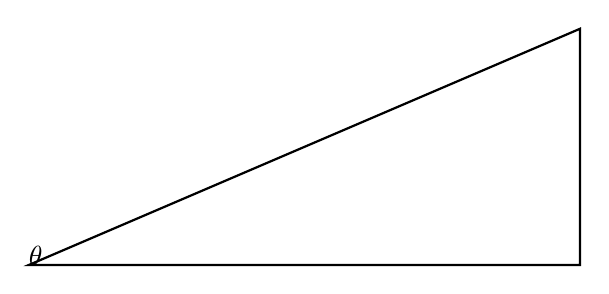
\begin{tikzpicture}[thick]
\coordinate (O) at (0,0);
\coordinate (A) at (7,0);
\coordinate (B) at (7,3);
\draw (O)--(A)--(B)--cycle;

%\tkzLabelSegment[below=2pt](O,A){\textit{adjacent leg}}
%\tkzLabelSegment[left=2pt](O,B){\textit{hypotenuse}}
%\tkzLabelSegment[above right=2pt](A,B){\textit{opposite leg}}

\tkzLabelSegment[below=5pt](O,A){\textit{x}}
\tkzLabelSegment[above left=5pt](O,B){\textit{r}}
\tkzLabelSegment[right=5pt](A,B){\textit{y}}

\tkzMarkAngle[fill= orange,size=1.5cm, opacity=.4](A,O,B)
\tkzLabelAngle[pos = 2](A,O,B){\texttt{$\theta$}}

% \tkzMarkAngle[fill= orange,size=0.65cm, opacity=.4](A,O,B)
% \tkzLabelAngle[pos = 0.35](A,O,B){$\gamma$}
%
% \tkzMarkAngle[fill= orange,size=0.8cm, opacity=.4](B,A,O)
% \tkzLabelAngle[pos = 0.6](B,A,O){$\alpha$}
%
% \tkzMarkAngle[fill= orange,size=0.7cm, opacity=.4](O,B,A)
% \tkzLabelAngle[pos = 0.5](O,B,A){$\beta$}

\end{tikzpicture}

\item Du har nytta av metoderna \code{math.cos(theta)} och \code{math.sin(theta)} vid omvandling från polära koordinater.

\item Attributet \code{negY} kommer att underlätta för dig när du på laborationen ska omvandla en punkt till fönsterkoordinater där y-axeln är omvänd jämfört med kartesiska koordinater.

\item Notera att klassens attribut är av typen \code{Double} och inte \code{Int}, trots att vi senare ska använda punkten för att beskriva en diskret pixelposition. Anledningen till detta är att det kan uppstå avrundningsfel vid numeriska beräkningar. Detta blir särskilt märkbart vid upprepad räkning med små värden, t.ex. när man ritar en approximerad cirkel med många linjesegment.
\end{itemize}

\SOLUTION

\TaskSolved \what~
\begin{Code}
package graphics

case class Point(x: Double, y: Double) {
  val r: Double          = math.hypot(x, y)
  val theta: Double      = math.atan2(y, x)
  def negY: Point        = Point(x, -y)
  def +(p: Point): Point = Point(x + p.x, y + p.y)
}
object Point {
  def polar(r: Double, theta: Double): Point =
    Point(r * math.cos(theta), r * math.sin(theta))
}
\end{Code}

\QUESTEND



\clearpage

\ExtraTasks %%%%%%%%%%%%%%%%%%%%%%%%%%%%%%%%%%%%%%%%%%%%%%%%%%%%%%%%%%%%%%%%%%%%



\WHAT{Instansiering med \code{new} och värdet \code{null}.}

\QUESTBEGIN

\Task  \what~  Man skapar instanser av klasser med \code{new}. Då anropas konstruktorn och plats reserveras i datorns minne för objektet. Variabler av referenstyp som inte refererar till något objekt har värdet \code{null}.

\Subtask Vad händer nedan? Vilka rader ger felmeddelande och i så fall hur lyder felmeddelandet?

\begin{REPL}
scala> class Gurka(val vikt: Int)
scala> var g: Gurka = null
scala> g.vikt
scala> g = new Gurka(42)
scala> g.vikt
scala> g = null
scala> g.vikt
\end{REPL}

\Subtask Rita minnessituationen efter raderna 2, 4, 6.

\SOLUTION


\TaskSolved \what


\SubtaskSolved  Rad 3 och 7 ger båda felmeddelandet \code{java.lang.NullPointerException},  på grund av försök att referera medlemmar med hjälp av en \code{null}-referens, som alltså inte pekar på något objekt.

\SubtaskSolved  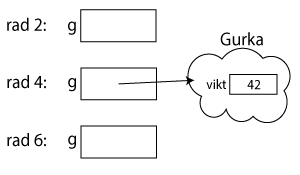
\includegraphics[scale=0.6]{../img/w06-solutions/1b}


\QUESTEND


\WHAT{Klasser,  instanser och skräp.}

\QUESTBEGIN

\Task  \what~För länge sedan i en galax långt långt borta...

\begin{Code}
case class Arm(ärTillVänster: Boolean)

case class Ben(ärTillVänster: Boolean)

case class Huvud(harHår: Boolean = true)

case class Rymdvarelse (
      arm1:   Arm   = Arm(true),
      arm2:   Arm   = Arm(false),
      ben1:   Ben   = Ben(true),
      ben2:   Ben   = Ben(false),
      huvud1: Huvud = Huvud(harHår = false),
  var huvud2: Huvud = Huvud()
) {
  def ärSkallig = !huvud1.harHår && !huvud2.harHår
}
\end{Code}

\Subtask Klistra in ovan rymdkod i REPL och evaluera nedan rader. Rita minnessituationen efter rad 5 och beskriv vad som händer.
\begin{REPL}
scala> val alien = Rymdvarelse()
scala> alien.ärSkallig
scala> val predator = Rymdvarelse()
scala> predator.ärSkallig
scala> predator.huvud2 = alien.huvud1
scala> predator.huvud2 eq alien.huvud1  // test av referenslikhet
scala> println(predator)
scala> predator.ärSkallig
\end{REPL}

\Subtask Vad händer så småningom med det ursprungliga \code{huvud2}-objektet i predator efter tilldelningen på rad 5? Går det att referera till detta objekt på något sätt?

\SOLUTION

\TaskSolved \what

\SubtaskSolved  Vi skapar två rymdvarelser, \code{alien} och \code{predator}, med vardera två ben och två armar, samt vardera två huvuden (där det ena är skalligt och det andra har hår). Efter det är varken \code{alien} eller \code{predator} skallig eftersom båda har ett huvud med hår. Sen låter man referensen till \code{predator}s huvud med hår referera till aliens huvud utan hår. Nu är predator helt skallig och delar huvud med alien.

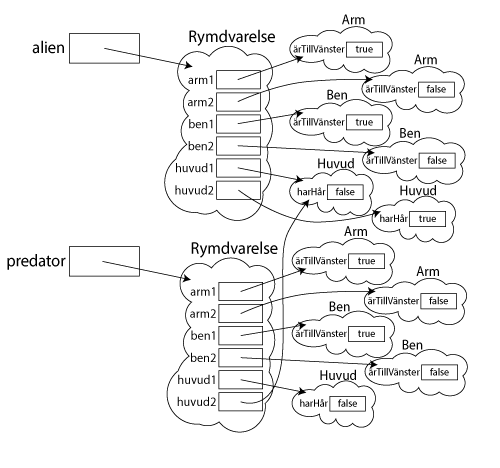
\includegraphics[scale=0.65]{../img/w06-solutions/2b}

\SubtaskSolved  Eftersom det inte längre finns någon referens som pekar på det objektet kommer skräpsamlaren att ta hand om det och det kommer förr eller senare skrivas över av något annat när platsen i minnet behövs. Objekt som inte har någon referens tills sig går inte att komma åt.

\QUESTEND




\WHAT{Case-klass. Oföränderlig kvadrat.}

\QUESTBEGIN

\Task \label{task:Square} \what~

\Subtask Implementera nedan kvadrat med en editor och klistra in den i REPL.

\begin{Code}
case class Square(val x: Int = 0, val y: Int = 0, val side: Int = 1) {
  val area: Int = ???

  /** Creates a new Square moved to position (x + dx, y + dy) */
  def moved(dx: Int, dy: Int): Square = ???

  def isEqualSizeAs(that: Square): Boolean = ???

  /** Multiplies the side with factor and rounded to nearest integer */
  def scale(factor: Double): Square = ???
}
object Square {
  /** A Square at (0, 0) with side 1 */
  val unit: Square = ???
}
\end{Code}

\Subtask Testa din kvadrat enligt nedan. Förklara vad som händer.

\begin{REPL}
scala> val (s1, s2) = (Square(), Square(1, 10, 1))
scala> val s3 = s1 moved (1,-5)
scala> s1 isEqualSizeAs s3
scala> s2 isEqualSizeAs s1
scala> s1 isEqualSizeAs Square.unit
scala> s2.scale(math.Pi) isEqualSizeAs s2
scala> s2.scale(math.Pi) isEqualSizeAs s2.scale(math.Pi)
scala> s2.scale(math.Pi) eq s2.scale(math.Pi)
scala> Square.unit eq Square.unit
\end{REPL}

\SOLUTION

\TaskSolved \what

\SubtaskSolved

\begin{Code}
case class Square(val x: Int = 0, val y: Int = 0, val side: Int = 1) {
	val area: Int = side * side

	def moved(dx: Int, dy: Int): Square = new Square(x + dx, y + dy, side)

	def isEqualSizeAs(that: Square): Boolean = this.side == that.side

	def scale(factor: Double): Square =
    Square(x, y, (side * factor).round.toInt)
}

object Square {
	val unit: Square = Square()
}
\end{Code}

\SubtaskSolved
\begin{REPL}
scala> val (s1, s2) = (Square(), Square(1, 10, 1))
s1: Square = Square(0,0,1)
s2: Square = Square(1,10,1)

scala> val s3 = s1 moved (1,-5)
s3: Square = Square(1,-5,1)

scala> s1 isEqualSizeAs s3       // lika storlek
res55: Boolean = true

scala> s2 isEqualSizeAs s1       // lika storlek
res56: Boolean = true

scala> s1 isEqualSizeAs Square.unit   // s1 har sidan 1
res57: Boolean = true

scala> s2.scale(math.Pi) isEqualSizeAs s2  // olika storlek
res58: Boolean = false

scala> s2.scale(math.Pi) == s2.scale(math.Pi) // lika innehåll
res59: Boolean = true

scala> s2.scale(math.Pi) eq s2.scale(math.Pi)  // olika objekt
res60: Boolean = false

scala> Square.unit eq Square.unit   // samma objekt
res61: Boolean = true
\end{REPL}

\QUESTEND



\WHAT{Förändrinsbar Java-klass.}

\QUESTBEGIN

\Task \what~Översätt nedan Scala-klass till Java-klassen \code{JMutablePoint3D}. Alla attribut ska vara privata (varför?). Översätt defaultargumentet till en alternativ konstruktor. Kalla setters för t.ex. \jcode{setX}. Kör \code{javac} och testa i REPL.

\begin{Code}
class MutablePoint3D(var x: Int, var y: Int, var z: Int = 0)
\end{Code}

\SOLUTION

\TaskSolved \what~

\javainputlisting[numbers=left]{examples/JMutablePoint3D.java}

\begin{REPL}
> atom JMutablePoint3D.java
> javac JMutablePoint3D.java
> ls
JMutablePoint3D.class  JMutablePoint3D.java
> scala
Welcome to Scala 2.12.3 (Java HotSpot(TM) 64-Bit Server VM, Java 1.8.0_121).
Type in expressions for evaluation. Or try :help.

scala> val p = new JMutablePoint3D(1,2)
p: JMutablePoint3D = JMutablePoint3D@2cae9b8

scala> p.x
<console>:13: error: value x is not a member of JPoint3D

scala> p.getZ
res0: Int = 0

scala> p.setZ(3)

scala> p.getZ
res1: Int = 3

\end{REPL}

\QUESTEND






\clearpage

\AdvancedTasks %%%%%%%%%%%%%%%%%%%%%%%%%%%%%%%%%%%%%%%%%%%%%%%%%%%%%%%%%%%%%%%%%


\WHAT{Attributrepresentation. Privat konstruktor. Fabriksmetod.}

\QUESTBEGIN

\Task \what~Kim Kodkunnig skapade för länge sedan denna klass som används på många ställen i befintlig kod:

\begin{Code}
class Point private (val x: Int, val y: Int)
object Point {
  def apply(x: Int = 0, y: Int = 0): Point = new Point(x, y)
  val origo = apply()
}
\end{Code}

\Subtask Vad händer om du försöker instansiera Kim Kodkunnigs klass direkt med nyckelordet \code{new}?

\Subtask Varför använder Kim Kodkunnig ett kompanjonsobjekt med en fabriksmetod? Vilka accessregler gäller mellan ett kompanjonsobjekt och klassen med samma namn?

\Subtask Hjälp Kim Kodkunnig att ändra attributrepresentationen så att det oföränderliga tillståndet utgörs av en 2-tupel \code{val p: (Int, Int)} i stället. Befintlig kod ska inte behöva ändras och klassen \code{Point} ska bete sig från ''utsidan'' precis som innan.

\SOLUTION

\TaskSolved \what~

\SubtaskSolved Det blir kompileringsfel eftersom konstruktorn är privat.
\begin{REPL}
scala> :paste

class Point private (val x: Int, val y: Int)
object Point {
  def apply(x: Int = 0, y: Int = 0): Point = new Point(x, y)
  val origo = apply()
}

scala> new Point(0,0)
<console>:14: error: constructor Point in class Point cannot be accessed
\end{REPL}

\SubtaskSolved
\begin{itemize}
  \item Genom att ha en privat konstruktor och bara göra indirekt instansiering via fabriksmetod är lätt ändra attributrepresentation i framtiden utan att befintlig kod behöver ändras.

  \item Med en \code{apply}-metod i kompansjonsobjektet kan man instansiera genom att skriva \code{Point(1, 2)} utan new.

  \item Accessreglerna för kompanjonsobjekt är sådana att kompanjoner ser varandras privata delar.
\end{itemize}

\SubtaskSolved

\begin{Code}
class Point private (private val p: (Int, Int)) {
  def x: Int = p._1
  def y: Int = p._2
}
object Point {
  def apply(x: Int = 0, y: Int = 0): Point = new Point(x, y)
  val origo = apply()
}
\end{Code}

\QUESTEND



\WHAT{Synlighet av klassparametrar och konstruktor, \code{private[this]}.}

\QUESTBEGIN

\Task  \what~

\Subtask En av gurk-klasserna nedan är trasig. Varför och vad blir det för fel?

\begin{Code}
class Gurka1(vikt: Int)

class Gurka2(val vikt: Int)

class Gurka3(private val vikt: Int)

class Gurka4(private val vikt: Int, kompis: Gurka4){
  def kompisVikt = kompis.vikt
}

class Gurka5(private[this] val vikt: Int, kompis: Gurka5){
  def kompisVikt = kompis.vikt
}

class Gurka6 private (vikt: Int)

class Gurka7 private (var vikt: Int)
object Gurka7 {
  def apply(vikt: Int) = {
    require(vikt >= 0, "negativ vikt: " + vikt)
    new Gurka7(vikt)
  }
}
\end{Code}

\Subtask Undersök nedan vad nyckelorden \code{val} och \code{private} får för konsekvenser. Förklara vad som händer. Vilka rader ger vilka felmeddelanden?

\begin{REPL}
scala> new Gurka1(42).vikt
scala> new Gurka2(42).vikt
scala> new Gurka3(42).vikt
scala> val ingenGurka: Gurka4 = null
scala> new Gurka4(42, ingenGurka).kompisVikt
scala> new Gurka4(42, new Gurka4(84, null)).kompisVikt
scala> new Gurka6(42)
scala> new Gurka7(-42)
scala> Gurka7(-42)
scala> val g = Gurka7(42)
scala> g.vikt
scala> g.vikt = -1
scala> g.vikt
\end{REPL}


\SOLUTION


\TaskSolved \what

\SubtaskSolved \code{Gurka5} är trasig. Eftersom vikten i \code{Gurka5} är privat för instansen och inte klassen kan en instans inte accessa en annan instans vikt.
\begin{REPL}
  error: value vikt is not a member of Gurka5
  def kompisVikt = kompis.vikt
\end{REPL}


\SubtaskSolved
\begin{REPL}
scala> new Gurka1(42).vikt
<console>:13: error: value vikt is not a member of Gurka1
       new Gurka1(42).vikt
                      ^

scala> new Gurka2(42).vikt
res64: Int = 42

scala> new Gurka3(42).vikt
<console>:13: error: value vikt in class Gurka3 cannot be accessed in Gurka3
       new Gurka3(42).vikt
                      ^

scala> val ingenGurka: Gurka4 = null
ingenGurka: Gurka4 = null

scala> new Gurka4(42, ingenGurka).kompisVikt
java.lang.NullPointerException
  at Gurka4.kompisVikt(<console>:13)
  ... 36 elided

scala> new Gurka4(42, new Gurka4(84, null)).kompisVikt
res67: Int = 84

scala> new Gurka6(42)
<console>:13: error: constructor Gurka6 in class Gurka6 cannot be accessed
       new Gurka6(42)
       ^

scala> new Gurka7(-42)
<console>:14: error: constructor Gurka7 in class Gurka7 cannot be accessed
       new Gurka7(-42)
       ^

scala> Gurka7(-42)
java.lang.IllegalArgumentException: requirement failed: negativ vikt: -42


scala> val g = Gurka7(42)
g: Gurka7 = Gurka7@70717ed5

scala> g.vikt
res71: Int = 42

scala> g.vikt = -1
g.vikt: Int = -1

scala> g.vikt
res72: Int = -1
\end{REPL}

\QUESTEND





\WHAT{Egendefinierad setter kombinerat med privat konstruktor.}

\QUESTBEGIN

\Task  \what~Klistra in denna kod i REPL:

\begin{Code}
class Gurka8 private (private var _vikt: Int) {
  def vikt = _vikt
  def vikt_=(v: Int): Unit = {
    require(v >= 0, "negativ vikt: " +v)
    _vikt = v
  }
}

object Gurka8 {
  def apply(vikt: Int) = {
    require(vikt >= 0, "negativ vikt: " + vikt)
    new Gurka8(vikt)
  }
}
\end{Code}


\Subtask Förklara vad som händer nedan. Vilka rader ger vilka felmeddelanden?
\begin{REPL}
scala> val g = Gurka8(-42)
scala> val g = Gurka8(42)
scala> g.vikt
scala> g.vikt = 0
scala> g.vikt = -1
scala> g.vikt += 42
scala> g.vikt -= 1000
\end{REPL}

\Subtask Vad är fördelen med möjligheten att skapa egendefinierade setters?

\SOLUTION


\TaskSolved \what


\SubtaskSolved

Rad 1:
\begin{REPL}
	java.lang.IllegalArgumentException: requirement failed: negativ vikt: -42
\end{REPL}
\code{Gurka8.apply} kräver att \code{vikt >= 0} annars kastar \code{require} ett undantag.

Rad 5:
\begin{REPL}
	java.lang.IllegalArgumentException: requirement failed: negativ vikt: -1
\end{REPL}
Settern \code{vikt_=} kräver att \code{vikt >= 0} annars kastar \code{require} ett undantag.

Rad 7:
\begin{REPL}
	java.lang.IllegalArgumentException: requirement failed: negativ vikt: -958
\end{REPL}
Eftersom \code{42 - 1000} är mindre än noll kastar \code{require} ett undantag.

\SubtaskSolved  Man kan sätta egna mer specifika krav på vad som får göras med värdena så man har större koll på att inget oväntat händer.

\QUESTEND




\WHAT{Objekt med föränderligt tillstånd \Eng{mutable state}.}

\QUESTBEGIN

\Task  \what~  Du ska implementera en modell av en hoppande groda som uppfyller följande krav:
\begin{enumerate}%[nolistsep, noitemsep]
\item Varje grodobjekt ska hålla reda på var den är.
\item Varje grodobjekt ska hålla reda på hur långt grodan hoppat totalt.
\item Varje grodobjekt ska kunna beräkna hur långt det är mellan grodans nuvarande position och utgångsläget.
\item Alla grodor börjar sitt hoppande i origo.
\item En groda kan hoppa enligt två metoder:
  \begin{itemize} [nolistsep, noitemsep]
  \item relativ förflyttning enligt parametrarna \code{dx} och \code{dy},
  \item slumpmässig relativ förflyttning $[1, 10]$ i x-ledsförändring och $[1, 10]$ i y-ledsförändring.
  \end{itemize}
\end{enumerate}

\Subtask Implementera klassen \code{Frog} enligt nedan kodskelett och ovan krav.

\begin{Code}
class Frog private (initX: Int = 0, initY: Int = 0) {
  def x: Int = ???
  def y: Int = ???

  def jump(dx: Int, dy: Int): Unit = ???
  def randomJump: Unit = ???

  def distanceToStart: Double = ???
  def distanceJumped: Double = ???
  def distanceTo(that: Frog): Double = ???
}
object Frog {
  def spawn(): Frog = ???
}
\end{Code}
\emph{Tips:}
\begin{itemize} [nolistsep, noitemsep]
\item Om namnet man vill ge ett privat föränderligt attribut ''krockar'' med ett metodnamn, är det vanligt att man börjar attributets namn med understreck, t.ex. \code{private var _x } för att på så sätt undkomma namnkonflikten.
\item Inför en metod i taget och klistra in den nya grodan i REPL efter varje utvidgning och testa.
\end{itemize}



\Subtask Skapa en metod \code{def test(): Unit} i ett singelobjekt \code{FrogTest} som innehåller kod som gör minst en kontroll av varje krav. Om ingen kontroll går fel ska \code{"Test Ok!"} skrivas ut annars ska exekveringen avbrytas. \emph{Tips:} Använd \code{assert(b, msg)} som avbryter exekveringen och skriver ut \code{msg} om \code{b} är falsk.

\Subtask Vad kallas en metod som enbart returnerar värdet av ett privat attribut?

\Subtask Inför setters för attributen som håller reda på x- och y-postitionen. Förändringar av positionen i x- eller y-led ska räknas som ett hopp och alltså registreras i det attribut som håller reda på det ackumulerade hoppavståndet.

\Subtask Simulera ett massivt grodhoppande med krockdetektering genom att skapa 100 grodor som till att börja med är placerade på x-axeln med avståndet $8$ längdenheter mellan sig. För varje runda i en \code{while}-sats, låt en slumpässigt vald groda göra ett \code{randomJump} tills någon groda befinner sig närmare än $0.5$ längdenheter, vilket är definitionen på att de har krockat. Räkna hur många looprundor som behövs innan något grodpar krockar och skriv ut antalet. Skriv även ut det totala antalet \\ \emph{Tips:} Börja med pseudokod på papper. Använd en grodvektor.


\SOLUTION


\TaskSolved \what


\SubtaskSolved
\begin{Code}
class Frog private (initX: Int = 0, initY: Int = 0) {
	private var _x: Int = initX
	private var _y: Int = initY
	private var _distanceJumped: Double = 0

  def x: Int = _x
  def y: Int = _y

	def jump(dx: Int, dy: Int): Unit = {
		_x += dx
		_y += dy
		_distanceJumped += math.hypot(dx, dy)
	}


	def randomJump: Unit = {
		def rnd = util.Random.nextInt(10) + 1
		jump(rnd, rnd)
	}

	def distanceToStart: Double = math.hypot(x,y)
	def distanceJumped: Double = _distanceJumped
	def distanceTo(f: Frog): Double = math.hypot(x - f.x, y - f.y)
}

object Frog {
	def spawn(): Frog = new Frog()
}
\end{Code}

\SubtaskSolved Exempel på testprogram:
\begin{Code}
object FrogTest {
  def test(): Unit = {
    val f1 = Frog.spawn()
    assert(f1.x == 0 && f1.y == 0, "Test of spawn, reqt 1 & 4 failed.")

    f1.jump(4,3)
    assert(f1.x == 4 && f1.y == 3, "Test of jump, reqt 1 & 4 failed.")

    f1.jump(4,3)
    assert(f1.distanceJumped == 10, "Test of jump, reqt 2 failed.")

    f1.jump(-4,-3)
    assert(f1.distanceToStart == 5, "Test of jump, reqt 3 failed.")

    for (x <- 1 to 10000) {
      val f2 = Frog.spawn()
    	f2.randomJump
    	assert(f2.x > 0 && f2.x <= 10 && f2.y > 0 && f2.y <= 10,
            "Test of randomJump, reqt 5 failed.")
    }
    println("Test Ok!")
  }
}
\end{Code}

\SubtaskSolved  En metod som är en indirekt avläsning av attrubtvärden kallas getter.

\SubtaskSolved
\begin{Code}

class Frog private (initX: Int = 0, initY: Int = 0) {
	private var _x: Int = initX
	private var _y: Int = initY
	private var _distanceJumped: Double = 0

	def jump(dx: Int, dy: Int): Unit = {
		_x += dx
		_y += dy
		_distanceJumped += math.hypot(dx, dy)
	}

	def x: Int = _x
  def x_= (newX: Int): Unit = { // Setter för x
		_distanceJumped += math.abs(x - newX)
		_x = newX
	}

  def y: Int = _y
	def y_= (newY: Int): Unit = { // Setter för y
		_distanceJumped += math.abs(y - newY)
		_y = newY
	}


	def randomJump: Unit = {
		def rnd = util.Random.nextInt(10) + 1
		jump(rnd, rnd)
	}

	def distanceToStart: Double = math.hypot(x,y)
	def distanceJumped: Double = _distanceJumped
	def distanceTo(f: Frog): Double = math.hypot(x - f.x, y - f.y)
}

object Frog {
	def spawn(): Frog = new Frog()
}

\end{Code}

\SubtaskSolved
\begin{Code}
object frogSimulation {
  def isAnyCollision(frogs: Vector[Frog]): Boolean = {
    var found = false
    frogs.indices.foreach { i =>  // generate all pairs (i,j)
      for (j <- i + 1 until frogs.size)
        if (!found) found = frogs(i).distanceTo(frogs(j)) <= 0.5
    }
    found
  }

  def jumpUntilCrash(n: Int = 100, initDist: Int = 8): (Int, Double) = {
    val frogs = Vector.fill(n)(Frog.spawn)
    (0 until n).foreach(i => frogs(i).x = i * initDistance)
    var count = 0
    while (!isAnyCollision(frogs)) {
      frogs(util.Random.nextInt(n)).randomJump
    	count += 1
    }
    (count, frogs.map(_.distanceJumped).sum)
  }

  def run(nbrOfCrashTests: Int = 10) = for (i <- 1 to nbrOfCrashTests) {
    val (n, dist) = jumpUntilCrash()
    println(s"\nAntalet looprundor innan grodkrock: $n")
    println(s"Totalt avstånd hoppat av alla grodor: $dist")
  }
}
\end{Code}

\QUESTEND




\QUESTBEGIN

\Task  \what~  Webbshoppen \textbf{UberSquare} säljer flyttbara kvadrater. I affärsmodellen ingår att ta betalt per förflyttning. Du ska hjälpa UberSquare att utveckla en enkel prototyp för att imponera på riskkapitalister.

\Subtask Implementera \code{Square} enligt dokumentationskommentarerna i efterföljande kodskiss och enligt dessa krav:

\begin{enumerate}%[nolistsep, noitemsep]
   \item Varje instans av \code{Square} ska räkna antalet förflyttningar som gjorts sedan instansen konstruerats.

   \item För att kunna övervaka sina kunder vill UberSquare även räkna det totala antalet förflyttningar som gjorts av alla kvadrater som någonsin skapats (s.k. \emph{big data}).

  \item Varje gång förflyttning sker ska ett visst belopp adderas till den ackumulerade kostnaden för respektive kvadrat, enligt kostnadsberäkningen i krav 4.

  \item UberSquare är oroliga för att kvadraterna flyttas för långt bort och bestämmer därför att för varje förflyttning ska den ackumulerade kvadratkostnaden ökas med den nya positionens avstånd till ursprungsläget vid kvadratens konstruktion multiplicerat med aktuell storlek på kvadraten.

  \item För att framstå som goda berättar UberSquare i sin marknadsföring att skala är gratis att använda. \footnote{D.v.s ett anrop av metoden \code{scale} orsakar ingen omedelbar kostnad.}
\end{enumerate}

\begin{CodeSmall}
/** A mutable and expensive Square. */
class Square private (val initX: Int, val initY: Int, val initSide: Int) {
  private var nMoves = 0;
  private var sumCost = 0.0;

  private var _x = initX;
  private var _y = initY;

  private var _side = initSide;

  private def addCost(): Unit = {
   sumCost += ???
  }

  def x: Int = ???
  def y: Int = ???

  def side = ???

  /** Scales the side of this square and rounds it to nearest integer */
  def scale(factor: Double): Unit = ???

  /** Moves this square to position (x + xd, y + dy) */
  def move(dx: Int, dy: Int): Unit = ???

  /** Moves this square to position (x, y) */
  def moveTo(x: Int, y: Int): Unit = ???

  /** The accumulated cost of this Square */
  def cost: Double = ???

  /** Returns the accumulated cost. Sets the accumulated cost to zero. */
  def pay: Double = ???

  override def toString: String =
    s"Square[($x, $y), side: $side, #moves: $nMoves times, cost: $sumCost]"
}


object Square {
  private var created = Vector[Square]()

  /** Constructs a new Square object at (x, y) with size side */
  def apply(x: Int, y: Int, side: Int): Square = {
    require(side >= 0, s"side must be positive: $side")
    ???
  }

  /** Constructs a new Square object at (0, 0) with side 1 */
  def apply(): Square = ???

  /** The total number of moves that have been made for all squares. */
  def totalNumberOfMoves: Int = ???

  /** The total cost of all squares. */
  def totalCost: Double = ???
}
\end{CodeSmall}

\Subtask Testa din kvadratprototyp i REPL. Använd t.ex. koden nedan:
\begin{REPL}
scala> val xs = Vector.fill(10)(Square())
scala> xs.foreach(_.move(2, 3))
scala> xs.foreach(_.scale(2.9))
scala> val (m, c) = (Square.totalNumberOfMoves, Square.totalCost)
m: Int = 10
c: Double = 36.055512754639885
\end{REPL}

\SOLUTION

\TaskSolved \what~

\begin{CodeSmall}
class Square private (val initX: Int, val initY: Int, val initSide: Int) {
  private var nMoves = 0;
  private var sumCost = 0.0;

  private var _x = initX;
  private var _y = initY;

  private var _side = initSide;

  private def addCost(): Unit = {
   sumCost += math.hypot(x - initX, y - initY) * side
  }

  def x: Int = _x
  def y: Int = _y

  def side = _side

  def scale(factor: Double): Unit = { _side = (_side * factor).round.toInt }

  def move(dx: Int, dy: Int): Unit = {
    _x += dx; _y += dy;
    nMoves += 1
    addCost()
  }

  def moveTo(x: Int, y: Int): Unit = {
    _x = x; _y = y;
    nMoves += 1
    addCost()
  }

  def cost: Double = sumCost

  def pay: Double = {val temp = sumCost; sumCost = 0; temp}

  override def toString: String =
    s"Square[($x, $y), side: $side, #moves: $nMoves times, cost: $sumCost]"
}
object Square {
  private var created = Vector[Square]()

  def apply(x: Int, y: Int, side: Int): Square = {
    require(side >= 0, s"side must be positive: $side")
    val sq = (new Square(x, y, side))
    created :+= sq
    sq
  }

  def apply(): Square = apply(0, 0, 1)

  def totalNumberOfMoves: Int = created.map(_.nMoves).sum

  def totalCost: Double = created.map(_.cost).sum
}
\end{CodeSmall}

\QUESTEND



\WHAT{Hjälpkonstruktor.}

\QUESTBEGIN

\Task\Uberkurs \label{task:aux-constructor} \what~I tidigare uppgifter har vi möjliggjort alternativa sätt att skapa instanser genom default-argument och fabriksmetoder i kompanjonsobjekt.

Ett annat sätt att göras detta på, som i Scala är ovanligt\footnote{Men i Java är detta mycket vanligt då defaultargument m.m. inte ingår i språket.}, är att definiera flera konstruktorer inne i klasskroppen. I Scala kallas en sådan extra konstruktor för \textbf{hjälpkonstruktor} \Eng{auxiliary constructor}.

En hjälpkonstruktor skapar man i Scala genom att definiera en metod som har det speciella namnet \code{this}, alltså en deklaration \code{def this(...) = ...} Hjälpkonstruktorer måste börja med att anropa en annan konstruktor, antingen den primära konstruktorn (d.v.s. den som klasshuvudet definierar) eller en tidigare definierad  hjälpkonstruktor.

\Subtask Läs mer om hjälpkonstruktorer här: \\ \href{http://www.artima.com/pins1ed/functional-objects.html#6.7}{www.artima.com/pins1ed/functional-objects.html\#6.7}

\Subtask Hitta på en egen uppgift med hjälpkonstruktorer, baserat på någon av klasserna i tidigare övningar.


%\Task \TODO \\ \code{class Rational private (numerator: BigInt, denominator: BigInt)} \\
%Inspirerat av Rational i pins1ed med GCD\SOLUTION

\QUESTEND

%!TEX encoding = UTF-8 Unicode

%!TEX root = ../compendium2.tex

\Lab{\LabWeekFIVE}

\begin{Goals}
%!TEX encoding = UTF-8 Unicode

%!TEX root = ../compendium2.tex

\item Kunna skapa en klass utifrån en textuell beskrivning. % av dess medlemmar.
%\item Kunna skapa en klass utifrån ofärdig kod och dokumentationskommentarer.
%\item Kunna införa privata attribut med lämpliga namn som representerar instansers förändringsbara tillstånd.
\item Kunna förklara skillnaden mellan klasser och instanser av klasser.
\item Kunna förklara skillnader och likheter mellan ett singelobjekt och objekt som är instanser av klasser.
\item Kunna förklara skillnaden mellan förändringsbara och oföränderliga objekt.
%\item Förstå innebörden av instansreferensen \code{this}.
\item Kunna skapa och använda klasser vars instanser innehåller referenser till andra instanser (aggregering).

\end{Goals}

\begin{Preparations}
\item \DoExercise{\ExeWeekFIVE}{05}

\item Läs igenom hela laborationen och studera dokumentationen för:
\begin{itemize}[nolistsep,noitemsep]
\item klassen \jcode{SimpleWindow} här: \url{http://cs.lth.se/pgk/api/}

\item \code{scala.Double} och \code{scala.math}, speciellt metoder för avrunding, trigonometri och polära koordinater, här:
\url{http://www.scala-lang.org/api/current/} 
\end{itemize}

\end{Preparations}

\subsection{Bakgrund}

Under den här laborationen ska du skapa en samling av klasser som tillsammans kan användas för att rita i ett fönster. Du ska bland annat skapa en klass \code{Turtle} som använder den färdigskrivna java-klassen \code{SimpleWindow} för att möjliggöra sköldpaddsgrafik liknande det vi gjorde i kojo-laborationen i avsnitt \ref{section:lab:kojo}. 

%SimpleWindow kan skapa ett enkelt ritfönster på skärmen, med metoder för att rita linjer, etc. SimpleWindow håller koll på en ''penna'' som representerar \textit{aktuell ritposition}. Det finns metoder för att flytta pennan och att rita en rak linje från pennans aktuella ritposition till en ny pennposition. 
%Delar av dokumentationen för SimpleWindow återspeglas i nedan specifikation. 
%Den fullständiga dokumentationen återfinns här: \url{http://cs.lth.se/pgk/api/}

%\vspace{1em}%hack to keep comment with method
%\begin{JavaSpec}{class SimpleWindow}
%  /** mouse click event type */
%	public final static int MOUSE_EVENT = 1;
%
%  /** key pressed event type */
%	public final static int KEY_EVENT = 2;
%
%  /** window closed event type */
%	public final static int CLOSE_EVENT = 3;
%
%  /** Creates a window and makes it visible. */
%	public SimpleWindow(int width, int height, String title);
%
%  /** Returns the width of the window. */
%	public int getWidth();
%
%	/** Returns the height of the window. */
%	public int getHeight();
%
%	/** Clears the window. */
%	public void clear();
%
%	/** Closes the window.*/
%	public void close();
%
%	/** Opens the window. */
%	public void open();
%
%	/** Moves the pen to a new position. */
%	public void moveTo(int x, int y) ;
%
%	/** Moves the pen to a new position while drawing a line. */
%	public void lineTo(int x, int y);
%
%	/** Writes a string at the current position.* /
%	public void writeText(String txt);
%
%	/** Draws a bitmap image at the current position.*/
%	public void drawImage(Image image);
%
%	/** Returns the pen's x coordinate. */
%	public int getX();
%
%	/** Returns the pen's y coordinate. */
%	public int getY();
%
%	/** Sets the line width.  */
%	public void setLineWidth(int width);
%
%	/** Sets the line color. */
%	public void setLineColor(Color col);
%
%	/**Returns the current line width. */
%	public int getLineWidth();
%
%	/** Returns the current line color. */
%	public Color getLineColor();
%
%	/**  Waits for a mouse click. */
%	public void waitForMouseClick();
%
%	/** Returns the mouse x coordinate at the last mouse click. */
%	public int getMouseX();
%
%	/** Returns the mouse y coordinate at the last mouse click. */
%	public int getMouseY();
%
%	/**Adds a sprite to the window. */
%	public void addSprite(Sprite sprite);
%
%	/** Wait for a specified time. */
%	public static void delay(int ms);
%\end{JavaSpec}
%
%
%\clearpage

\subsection{Obligatoriska uppgifter}


\Task Skapa dessa kataloger %(kallas även bibliotek eller mappar på svenska och \emph{''folder''} eller \emph{directory} på engelska) 
och tomma filer för din kod med hjälp av nedan linuxkommandon (eller motsvarande på annat lämpligt sätt):
\begin{REPLnonum}
mkdir turtle
cd turtle
mkdir -p src/main/scala/graphics
touch Point.scala Main.scala 
mv *.scala src/main/scala/graphics/.
ls src/main/scala/graphics/
\end{REPLnonum}
Om man skriver mycket kod blir det lättare att hitta olika delar om man har dem i olika filer med lämpliga  filnamn. Det är vanligt att man lägger kodfilerna i katalogen \code{src/main/scala} och där skapar en egen underkatalog för varje paket med samma namn som paketet.\footnote{Flera verktyg kräver exakt denna katalogstruktur för att hitta koden utan specialinställningar.} 


\Task Du ska skapa case-klassen \code{Point} som ska beskriva en koordinat i ett kartesiskt koordinatsystem\footnote{\url{https://sv.wikipedia.org/wiki/Kartesiskt_koordinatsystem}}. Skapa kod med hjälp av en editor, t.ex. \code{atom}, i filen  \code{src/main/scala/graphics/Point.scala} enligt följande riktlinjer:
\begin{enumerate}%[noitemsep]
\item Klassen \code{Point} ska vara en oföränderlig case-klass. 

\item Klassen \code{Point} ska ligga i paketet \code{graphics}.

\item Klassen \code{Point} ska ha följande två publika, oföränderliga klassparametrar:
\begin{itemize}[nolistsep, noitemsep]
\item \code{x: Double} för x-koordinaten.
\item \code{y: Double} för y-koordinaten.
\end{itemize}

\item Klassen \code{Point} ska ha följande publika medlemmar (två oföränderliga attribut och två metoder):
\begin{itemize}[nolistsep, noitemsep]
\item \code{val r: Double} ska ge motsvarande polära kordinatens%
\footnote{\url{https://sv.wikipedia.org/wiki/Pol\%C3\%A4ra\_koordinater}}
 avstånd till origo.
\item \code{val theta: Double} ska ge polära kordinatens vinkel i radianer.
\item \code{def negY: Point} ska ge en ny punkt med y-koordinaten negerad. 
\item \code{def +(p: Point): Point} ska ge en ny punkt vars koordinat är summan av x- respektive y-kordinaterna för denna instans och punkten \code{p}.
\end{itemize}

\item Klassen \code{Point} ska ha ett kompanjonsobjekt med en metod som konstruerar en punkt från polära koortdinater. Metoden ska ha detta huvud: \\\code{def polar(r: Double, theta: Double): Point}

\end{enumerate}

\noindent Tips vid implementation och senare användning:
\begin{itemize}
\item Du har nytta av metoderna \code{math.hypot(x, y)} och \code{math.atan2(y, x)} vid omvandling till polära koordinater.

\item Du har nytta av metoderna \code{math.cos(x)} och \code{math.sin(y)} vid omvandling från polära koordinater.

\item Attributet \code{negY} kommer att underlätta för dig när du i metoden \code{draw} i klassen \code{Turtle} ska omvandla en punkt till fönsterkoordinater där y-axeln är omvänd jämfört med kartesiska koordinater.

\item Notera att klassens attribut är av typen \code{Double} och inte \code{Int}, trots att vi senare ska använda punkten för att beskriva en diskret pixelposition. Anledningen till detta är att det kan uppstå avrundningsfel vid numeriska beräkningar. Detta blir särskilt märkbart vid upprepad räkning med små värden, t.ex. när man ritar en approximerad cirkel med många linjesegment.
\end{itemize}

\noindent Du ska kunna använda din punkt enligt följande exempel. Starta REPL och klistra in din case-klass med sitt kompanjonsobjekt efter kommandot \code{:paste} (eller kortare \code{:pa}). Du ska inte ta med paketdeklarationen då \code{package} inte fungerar i REPL.
\begin{REPLnonum}
scala> Point(1,1).theta.toDegrees
res0: Double = 45.0

scala> Point(3,4).r
res1: Double = 5.0

scala> Point(1,1).negY + Point(2,5)
res2: Point = Point(3.0,4.0)

scala> Point.polar(2, 60.0.toRadians).theta.toDegrees
res3: Double = 60.000001669652114
\end{REPLnonum}


\Task Lägg \code{cslib.jar} i katalogen \code{lib}, t.ex. med dessa linuxkommandon:
\begin{REPLnonum}
$ mkdir lib
$ wget -O lib/cslib.jar http://cs.lth.se/pgk/cslib
\end{REPLnonum}

\Task Skapa en \code{main}-metod i singelobjektet \code{Main} i paketet \code{graphics} i filen \code{src/main/scala/graphics/Main.scala} som gör något enkelt med både \code{Point} och \code{SimpleWindow}, t.ex. drar en linje mellan två punkter enlig nedan. 
\scalainputlisting[numbers=left,basicstyle=\ttfamily\fontsize{11}{13}\selectfont]%
{../workspace/w05_turtle/src/main/scala/graphics/Main.scala}

\noindent När många kodfiler beror av varandra behöver kompilatorn ha tillgång till alla kodfiler samtidigt.  Detta kan åstadkommas genom att ge \code{*.scala} som argument till \code{scalac} enligt nedan. Dessutom blir det en hel del \code{.class}-filer som utdata från kompilatorn, så man brukar lägga dem i en katalog med namnet \code{bin} (eller ibland \code{target}) för att separera dem från övriga filer. Använd följande linuxkommando\footnote{I Windows, byt ut kolon mot semikolon.} för att skapa \code{bin}-katalog, samkompilera alla filer och köra \code{main}-metoden:
\begin{REPLnonum}
$ mkdir bin
$ scalac -cp lib/cslib.jar -d bin src/main/scala/graphics/*.scala
$ scala -cp "lib/cslib.jar:bin" graphics.Main
\end{REPLnonum}


\Task Skapa klassen Turtle som representerar en virtuell sköldpadda med en penna under magen som kan rita i \code{SimpleWindow} enligt nedan riktlinjer:

\begin{enumerate}
\item Klassen \code{Turtle} ska vara en klass med ett förändringsbart tillstånd bestående av tre privata attribut som håller reda på detta:

\begin{itemize}
\item en position av typen \code{Point} där ett positivt y-värde räknas \emph{nedåt} i fönstret.
\item en riktning av typen \code{Double} som anges som en vinkel i grader  (och inte radianer), där ett positivt värde anger vinkeln motsols från x-axeln. 
\item ett läge på pennan av typen \code{Boolean} där \code{true} anger att pennan är nere.
\end{itemize}

\item Utgå från det ofärdiga kodskelettet nedan där dokumentationskommentarerna ger ytterligare detaljer att ta hänsyn till. Om du skriver klassen från början behöver du inte skriva av dokumentationskommentarerna. Kodskelettet finns annars i kursens \code{workspace} på GitHub%
\footnote{\url{https://github.com/lunduniversity/introprog/blob/master/workspace/}} och här: \url{http://cs.lth.se/pgk/ws}

\item Flera metoder har \code{Turtle} som returtyp. I dessa fall ska en referens till den egna instansen returneras för att möjliggöra upprepad punktnotation, t.ex.:\\
\code{t.jumpTo(Point(100, 200)).turnNorth.penDown}

\scalainputlisting[numbers=left,basicstyle=\ttfamily\fontsize{10}{12}\selectfont]%
{../workspace/w05_turtle/src/main/scala/graphics/Turtle.scala}
\end{enumerate}

\noindent Tips:

\begin{itemize}
\item Allteftersom du implementerar de saknade delarna, utöka din \code{main}-metod i \code{Main.scala} med fler tester och kolla så att dina implementationer funkar som det är tänkt. Testa på nytt efter varje litet tillägg så att du hela tiden har något som fungerar. Det är mycket lättare att felsöka efter en liten ändring än efter många och stora ändringar.

\item Du får namnge de privata variablerna som representerar det förändringsbara tillståndet så som du själv anser lämpligt. Tänk på att det i Scala kan bli namnkrock mellan metoder och privata attribut. I dessa fall brukar man namnge det privata attributet med ett understreck före för att skilja dem åt, t.ex.: \\
\code{private var _direction: Double  = ???}

\item I metoden \code{forward} har du nytta av metoden \code{Point.polar}, metoden \code{.toRadians} som kan konvertera en \code{Double} i grader till radianer, samt metoden \code{negY}. Tänk på att vinkelberäkningar på radianer förutsätter kartesiskt koordinatsystem, så negeringen av Y-axeln ska ske efter sådana beräkningar, men innan uppdatering av positionen sker. 
\end{itemize}


\Task Implementera case-klassen \code{Rect} enligt specifikationen nedan. Kodskelettet finns i workspace. Testa dina implementationer allteftersom du skriver dem, genom att stegvis utöka din \code{main}-metod.

\scalainputlisting[numbers=left,basicstyle=\ttfamily\fontsize{10.5}{12}\selectfont]%
{../workspace/w05_turtle/src/main/scala/graphics/Rect.scala}

\noindent Metoderna ovan har \code{Rect} som returtyp; en referens till den egna instansen ska returneras för att möjliggöra upprepad punktnotation, t.ex.:\\
\code{r.rotatedLeft(15).translated(0, 2).scaled(1.5)}

\clearpage

\Task\Checkpoint När \code{Turtle} och \code{Rect} är färdigimplementerade så ska du testa klasserna gemensamt genom att köra \code{main}-metoden i singelobjektet \code{Demo} nedan. Koden finns i kursens workspace. 

Den första bilden ska visa två lika stora rektanglar i samma höjd. Efter musklick kommer en animering av tre färgglada rektanglar. När det finns en handledare ledig, redovisa vad du åstadkommit. Vid väntetid, fortsätt med efterföljande uppgifter.

\scalainputlisting[numbers=left,basicstyle=\ttfamily\fontsize{11}{14}\selectfont]%
{../workspace/w05_turtle/src/main/scala/graphics/Demo.scala}


\clearpage

\subsection{Frivilliga extrauppgifter}

Nedan uppgifter kan göras i valfri ordning.

\Task Använd din Turtle för att rita en cirkel. För att göra detta kan du t.ex. låta din Turtle gå ett kort steg och svänga någon grad tills den har gjort ett fullt varv.

\Task Skapa två stycken Turtles i samma fönsterobjekt som rör sig alternerande. Fungerar allt som tänkt?


\Task Studera dokumentationen för de \code{SimpleWindow}-metoder som erbjuder hantering av händelser \Eng{event} och använd dessa för lösa deluppgifterna nedan.

\Subtask Gör så att en Turtle kan styras med hjälp av tangentbordstryckningar A--S--D--W för vänster--ner--höger--upp och att den ritar ett spår allteftersom den förflyttas.

\Subtask Gör så att en andra Turtle kan styras med hjälp av tangentbordstryckningar J--K--L--I för vänster--ner--höger--upp och att den också ritar ett spår allteftersom den förflyttas.

\Subtask Gör så att, när de två sköldpaddorna ovan befinner sig tillräckligt nära varandra, det ritas ut en rektangel med hörn där de två sköldpaddorna finns. (Denna uppgift är lite svårare och kan behöva delas upp i delar.)


\Task Studera dokumentationen för de \code{SimpleWindow}-metoder som erbjuder hantering av flyttbara bilder \Eng{sprites}. Gör så att en fin Sprite ritas vid positionen för de styrbara sköldpaddorna i föregående uppgift.


\Task Skapa en case-klass \code{RectSeq} enligt specifikation på sidan \pageref{code:classes:graphics:rectanglesequence}. I denna klass skall metoden \code{draw} rita ut ett antal rektanglar där varje rektangel har förflyttat sig, roterats och skalats jämfört med föregående rektangel i sekvensen. 

\begin{figure}[H]
\centering
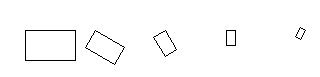
\includegraphics[width=0.75\textwidth]{../img/turtle/RectSeq.png}
%\caption Rotation av rektangel med koden nedan.
%\label{fig:classes:graphics:rollingrectangle}
\end{figure}
\noindent Bilden ovan kan skapas med hjälp av denna kod:
\begin{Code}
  def rectSeqExample(t: Turtle): Unit  = {
    val rect = Rect(pos = Point(200, 200), width = 50, height = 30)
    RectSeq(rect, n = 5, dist = 70, rot = -30, scale = 0.67).draw(t)
  }
\end{Code}

\noindent Nedan kod ritar bilden i fig. \ref{fig:classes:graphics:rectanglesequence} på sidan \pageref{fig:classes:graphics:rectanglesequence}. Använd gärna \code{setLineColor} i \code{SimpleWindow} för att göra en färggladare stjärna. Slumpvisa transformationer är också kul. 

\begin{Code}
val w = new SimpleWindow(500, 500, "Shapes")
val t = new Turtle(w, new Point(200, 200), 0, false)
val rect = Rect(pos = Point(225, 235), width = 50, height = 30)
val roll = RectSeq(rect, n = 100, dist = 2, scale = 0.98)
for (i <- 0 to 360 by 20) roll.rotatedLeft(i).draw(t)
\end{Code}


\begin{figure}
\centering
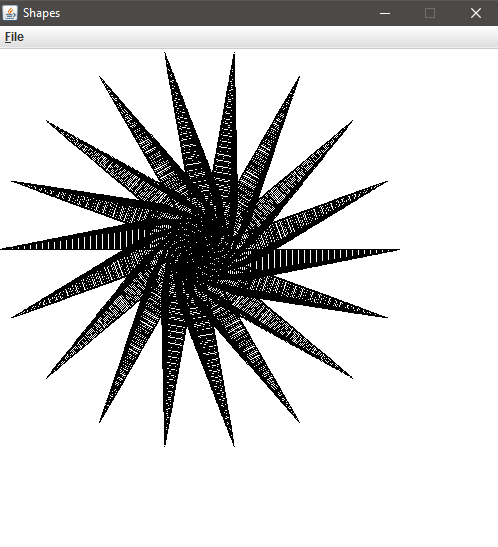
\includegraphics[width=0.5\textwidth]{../img/w06-lab/RectangleSequence.png}
\caption {En stjärna skapad med hjälp av \code{RectSeq}.}
\label{fig:classes:graphics:rectanglesequence}
\end{figure}

\noindent Nedan finns ett kodskellett som du kan utgå ifrån. Dokummentationskommentarerna innehåller fler detaljer om hur det är tänkt att klassen ska fungera. %De metoder som returnerar \code{RectSeq} ska returnera en referens till den egna instansen så att upprepad punktnotation möjliggörs.

\begin{figure}[H]
\scalainputlisting[numbers=left,basicstyle=\ttfamily\fontsize{9.9}{12}\selectfont]%
{../workspace/w05_turtle/src/main/scala/graphics/RectSeq.scala}
\label{code:classes:graphics:rectanglesequence}
\end{figure}



%\Task En riktig utmaning, för den som har lust: Implementera spelet ''Masken'' som beskrivs här: \url{https://sv.wikipedia.org/wiki/Snake}.


%!TEX encoding = UTF-8 Unicode

%!TEX root = ../compendium1.tex

%!TEX encoding = UTF-8 Unicode
\chapter{Sekvenser}\label{chapter:W06}
Begrepp som ingår i denna veckas studier:
\begin{multicols}{2}\begin{itemize}[noitemsep,label={$\square$},leftmargin=*]
\item översikt av Scalas samlingsbibliotek och samlingsmetoder
\item klasshierarkin i scala.collection
\item Traversable
\item Iterable
\item Seq
\item List
\item ListBuffer
\item ArrayBuffer
\item WrappedArray
\item sekvensalgoritm
\item algoritm: SEQ-COPY
\item in-place vs copy
\item algoritm: SEQ-REVERSE
\item registrering
\item algoritm: SEQ-REGISTER
\item linjärsökning
\item algoritm: LINEAR-SEARCH
\item tidskomplexitet
\item minneskomplexitet
\item sekvenser i Java vs Scala
\item for-sats i Java
\item java.util.Scanner
\item översikt strängmetoder
\item StringBuilder
\item ordning
\item inbyggda sökmetoder
\item find
\item indexOf
\item indexWhere
\item inbyggda sorteringsmetoder
\item sorted
\item sortWith
\item sortBy
\item variabelt argumentantal\end{itemize}\end{multicols}

\clearpage\section{Teori}
%!TEX encoding = UTF-8 Unicode
%!TEX root = ../lect-w06.tex

%%%

\ifkompendium\else
\Subsection{Veckans uppgifter}

\begin{SlideExtra}{Veckans övning: \texttt{patterns}}
  Mål: Träna på matchning och undantag
\begin{itemize}
\item Uppg. 1--8: Matchning, \code{Option}
\item Uppg. 9--11: Undantag, \code{Try}
\item Uppg. 12: Laborationsförberedelse \code{Cell} och \code{Table}
\item Uppg. 13: Matchning eller dynamisk bindning?
\item Uppg. 14: avgöra likhet med matchning, \code{equals} utan arv
\item Uppg. 15--22: diverse fördjupningsuppgifter om matchning, undantag, hash-koder, likhet vid arvshierarki
\end{itemize}
\end{SlideExtra}


\begin{SlideExtra}{Veckans labb: \texttt{tabular}}\SlideFontTiny
%  \setlength{\leftmargini}{0pt}
\hspace{-2em}\begin{minipage}{0.7\textwidth}
\vspace{0.25em}
\Emph{Förberedelse:}
\begin{itemize}
\item Gör övning \code{patterns}, speciellt uppg. 12
\item Studera givna koden: {\SlideFontTiny \href{https://github.com/lunduniversity/introprog/tree/master/workspace/w13_tabular}{workspace/w10\_tabular}}
\item Fyll i denna enkät:
\\{\SlideFontTiny \url{https://goo.gl/forms/hC6JK2UQXVpbGECc2}}
\item Se svar här (snapshot uppdateras då och då): \url{http://cs.lth.se/pgk/favorit}
\end{itemize}

\Emph{Grunduppgift:}
\begin{itemize}
\item Terminalapp för hantering av kolumndata i textfiler.
\item Matchning används vid kommandotolkning.
\item \code{Option} används för inkapsling av ev. saknade värden
\item \code{Try} används för inkapsling av ev. undantag
\end{itemize}
\Emph{Extrauppgifter:} (Minst en)
\begin{itemize}
\item dialoger: \code{load}, \code{save}, kommando: \code{pie}, \code{bar}
\end{itemize}
\end{minipage}
\hfill\begin{minipage}{0.3\textwidth}
\centering
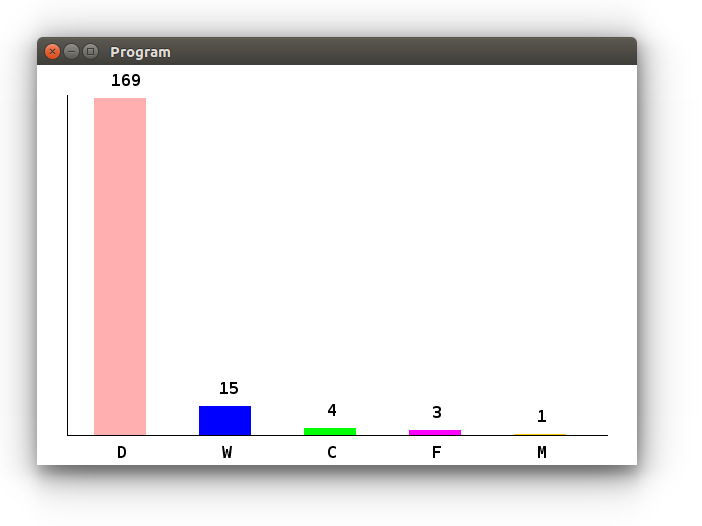
\includegraphics[width=0.95\textwidth]{../img/survey/bar}

\vspace{2em}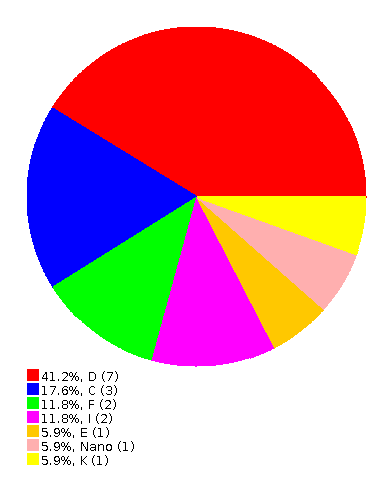
\includegraphics[width=0.7\textwidth]{../img/survey/pie}
\end{minipage}
\end{SlideExtra}

\begin{SlideExtra}{Extraundervisning del 3}
\begin{itemize}
\item  \Alert{Extraundervisning} i \Emph{E:1406} onsdag 21/11 kl 15:15-17:00
\item Hitta dit: \url{http://fileadmin.cs.lth.se/ehus/E1406.pdf}
\item Det finns gott om platser i den salen >70 platser så alla är välkomna
\item Fokus: grundläggande, långsam behandling på begäran, grumliga begrepp etc.
\end{itemize}
\end{SlideExtra}
\fi


%!TEX encoding = UTF-8 Unicode
%!TEX root = ../lect-w06.tex

%%%

\Subsection{Matchning}

\ifkompendium
\noindent  I ett match-uttryck kan man matcha på ett visst värde eller på en viss typ och match-uttryck används gärna istället för nästlade if-uttryck, då de ofta är lättare att läsa och begripa. Med match-uttryck kan man också göra \Emph{mönstermatchning} mot case-klass-instanser, t.ex. för att på ett smidigt sätt undersöka om attribut har speciella värden. Match-uttryck i Scala är en mer kraftfull variant av \code{switch}-satser som finns i många andra språk.  
\fi

\begin{Slide}{Vad är matchning?}

  \begin{itemize}
    \item Matchning gör man då man vill jämföra ett värde mot andra värden och hitta överensstämmelse \Eng{match} enligt olika \Emph{mönster}.
    \item Med mönster kan man även \Alert{plocka isär} objekt i sina beståndsdelar.
  \end{itemize}
\end{Slide}

\begin{Slide}{Plocka isär ett objekt i sina beståndsdelar med mönster}

\begin{REPLnonum}
scala> case class Point(x: Int, y: Int)

scala> val p = Point(1, 2)      // konstruera en punkt
val p: Point = Point(1,2)
\end{REPLnonum}

\pause 

~\\
\begin{REPLnonum}
scala> val Point(x, y) = p      // plocka isär en punkt
val x: Int = 1
val y: Int = 2
  
\end{REPLnonum}
\end{Slide}


\begin{Slide}{Kolla om det passar med nästlade if-then-else-uttryck}
Ett vanligt problem: \\ att kolla vilket bland många värden som passar \\~\\

Kan göras med nästlade if-then-else-uttryck:

\begin{Code}
val g = scala.io.StdIn.readLine("grönsak:")
val smak =
  if (g == "gurka") "gott!"
  else if (g == "tomat") "jättegott!"
  else if (g == "broccoli") "ganska gott..."
  else "inte gott :("

println(g + " är " + smak)
\end{Code}
      
\end{Slide}


\ifkompendium\else
\begin{SlideExtra}{Matchning är ungefär som att passa klossar i en låda}
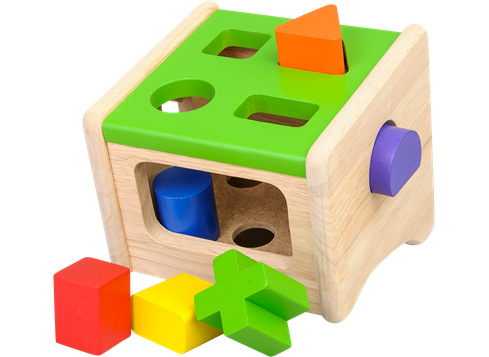
\includegraphics[width=0.8\textwidth]{../img/plocklada.png}
\end{SlideExtra}
\fi


\begin{Slide}{Kolla om det passar med \texttt{match}-uttryck}\SlideFontSmall
I stället för nästlade \code{if} kan du använda Scalas kraftfulla \code{match}-\Emph{uttryck}:

\begin{Code}
def g = scala.io.StdIn.readLine("Ange en grönsak: ")
def smak = g match 
  case "gurka"    => "gott!"
  case "tomat"    => "jättegott!"
  case "broccoli" => "ganska gott..."
  case _ => "mindre gott..."
\end{Code}
\begin{itemize}
\pause\item Varje \code{case}-gren testas var för sig i tur och ordning uppifrån och ned.
\item Det som står mellan \code{case} och \code{=>} kallas ett \Emph{mönster} \Eng{pattern}
\item Sista default-grenen ovan kallas \Emph{wildcard-mönster}: \code{case _ => }
\item Ovan är exempel på matchning mot \Emph{konstant-mönster}, \\ i detta fallet tre stycken strängkonstantmönster.
\item Det finns många andra sätt att skriva mönster.
\end{itemize}
% \pause Scalas \code{match} ''faller inte igenom'' som \code{switch}-satser som finns i många språk, t.ex. Java...

\end{Slide}


\begin{Slide}{Matchning med gard}
Man kan stoppa in en s.k \Emph{gard} \Eng{guard} innan pilen \code{=>} för att villkora matchningen: (notera \code{if} utan \code{then})
\begin{Code}
def g = scala.io.StdIn.readLine("Ange en grönsak: ")
def smak = g match 
  case "gurka" if math.random() > 0.5 => "gott ibland!"
  case "tomat" => "jättegott!"
  case "broccoli" => "ganska gott..."
  case _ => "mindre gott..."
\end{Code}
\code{case}-grenen med gard ger bara en lyckad matchning \\ om uttrycket efter \code{if} är sant; annars provas nästa gren, etc.
\end{Slide}

\begin{Slide}{Matchning med variabelmönster}\SlideFontSmall
Om det finns ett namn efter \code{case} som börjar med liten begynnelsebokstav, blir detta namn en variabel som automatiskt binds till uttrycket före \code{match}:

\begin{Code}
def g = scala.io.StdIn.readLine("Ange en grönsak: ")
def smak = g match 
  case "gurka" if math.random() > 0.5 => "gott ibland!"
  case "tomat" => "jättegott!"
  case "broccoli" => "ganska gott..."
  case other => "smakar bakvänt: " + other.reverse
\end{Code}

Ett enkelt variabelmönster, så som \\ \code{case other => ...} \\ i exemplet ovan, matchar \Emph{allt}! \\\code{other} får alltså värdet av \code{g} om \code{g} \Alert{inte} är \code{"gurka"}, \code{"tomat"}, \code{"broccoli"}.

\end{Slide}


\begin{Slide}{Matchning med eller-mönster}\SlideFontSmall
Om man har samma utfall för olika grenar kan dessa slås ihop och mönstret separeras med vertikalstreck: \code{|}
\begin{Code}
def g = scala.io.StdIn.readLine("Ange en grönsak: ")
def smak = g match 
  case "gurka" => "gott"
  case "tomat" => "gott"
  case "lök"   => "gott"
  case _ => "inte gott"
\end{Code}

Mer koncist med eller-mönster:

\begin{Code}
def g = scala.io.StdIn.readLine("grönsak:")
def smak = g match 
  case "gurka" | "tomat" | "lök" => "gott"
  case _ => "inte gott"
\end{Code}



\end{Slide}





\begin{Slide}{Matchning med typade mönster}\SlideFontSmall
Med en typannotering efter en variabel får man ett \Emph{typat mönster} \Eng{typed pattern}. Om matchningen lyckas blir värdet \Alert{omvandlat} till den specifika typen och binds till variabeln.
\begin{Code}
def f = 
  if (math.random() < 0.5) 42 + math.random() else "gurka" + math.random()

def g = f match 
  case x: Double => x.round.toInt
  case s: String => s.length
\end{Code}
\code{f} får typen \code{Matchable} som är subtyp till \code{Any}. Vilken typ får \code{g}? \pause ~~\code{Int}\\
Matchning mot specifika typer enl. ovan används i idiomatisk Scala hellre än \code{isInstanceOf} men man kan göra motsvarande ovan med detta if-uttryck:
\begin{Code}
def g2 =  
  val x = f
  val y = 
    if (x.isInstanceOf[Double]) x.asInstanceOf[Double].round.toInt
    else if (x.isInstanceOf[String]) x.asInstanceOf[String].length
  y.asInstanceOf[Int] // kan detta ge körtidsfel? kan kompilatorn kolla det?
\end{Code}
\end{Slide}

\begin{Slide}{Typen \text{Matchable}}
När ett uttryck inte kan ges en mer specifik typ så härleds \code{Matchable}, vilket visar att värdet kan undersökas med \code{match}.\footnote{Mer detaljer om varför \code{Matchable} behövs här: https://dotty.epfl.ch/docs/reference/other-new-features/matchable.html}
\begin{REPLnonum}
scala> def f = if math.random() > 0.5 then 42 else "hej"
def f: Matchable
\end{REPLnonum}
%Eftersom typen \code{String} och typen \code{Double} inte har något annat gemensamt bli den mest specifika typen som kan härledas \code{Matchable}, som är nästan lika generell som topptypen \code{Any}.
\end{Slide}

\begin{Slide}{Konstruktormönster med case-klasser}\SlideFontSmall
En basklass med gemensamma delar och två subtyper:
\begin{Code}
trait Grönsak:
  def vikt: Int
  def ärRutten: Boolean

case class Gurka(vikt: Int, ärRutten: Boolean) extends Grönsak
case class Tomat(vikt: Int, ärRutten: Boolean) extends Grönsak
\end{Code}
\pause
Tack vare case-klasserna kan man använda \Emph{konstruktormönster} \Eng{constructor pattern} för att se vad som finns \Alert{inuti} en instans:
\begin{Code}
def testa(g: Grönsak): String = g match 
  case Gurka(v, false) => "gott, väger " + v
  case Gurka(_, true)  => "inte gott"
  case Tomat(v, r)     => (if r then "inte " else "") + s"gott, väger $v"
  case _ => "okänd grönsak: $g"
\end{Code}

Konstruktormönster ''\Emph{plockar isär}'' det som matchas och binder variabler till de attribut som finns i case-klassens konstruktor.
\end{Slide}


\begin{Slide}{Plocka isär samlingar med djupa mönster}
Man kan plocka isär innehållet i en samling så här:
\begin{Code}
def visa(xs: Vector[Grönsak]): String = xs match
  case Vector()               => "tom grönsaksvektor"
  case Vector(Gurka(v, true)) => s"en rutten gurka som väger $v"
  case Vector(g)              => s"exakt en grönsak: $g"
  case Vector(g1, g2)         => s"exakt två grönsaker: $g1, $g2"
  case g +: gs                => s"först en $g och sedan svansen: $gs"
\end{Code}
Vad händer om du byter ordning på andra och tredje mönstret?
\end{Slide}

\begin{Slide}{Matchning på tupler}
Det går fint att plocka isär tupler med mönstermatchning:\footnote{\url{https://youtu.be/aboZctrHfK8}}
\begin{Code}
var pair = ("hej", 42)

pair match
  case (a, b) if b == 42 => s"livets mening är funnen: $a"
  case (_, b)            => s"fattas mening: $b"

\end{Code}

\end{Slide}

\begin{Slide}{Mönstermatchning och uppräkning med case-objekt}\SlideFontSmall
En bastyp och specifika singelobjekt av gemensam typ:
\begin{Code}
trait Färg
case object Spader  extends Färg // funkar utan case men vi vill ha najs toString
case object Hjärter extends Färg
case object Ruter   extends Färg
case object Klöver  extends Färg

def parallellFärg(f: Färg): Färg = f match
  case Spader  => Klöver
  case Klöver  => Spader
  case Hjärter => Ruter
\end{Code}
Vilken case-gren har vi glömt? Kan kompilatorn hjälpa oss?
\pause
\begin{REPL}
scala> parallellFärg(Ruter)
scala.MatchError: Ruter 
\end{REPL}
\Alert{Undantag vid körtid} \code{:(}
\end{Slide}

\begin{Slide}{Mönstermatchning och förseglade typer}\SlideFontSmall
Med nyckelordet \code{sealed} får vi en kompileringsvarning.
\begin{Code}
sealed trait Färg //tryck Alt+Enter i REPL för tolkning av flera rader ett svep
case object Spader  extends Färg
case object Hjärter extends Färg
case object Ruter   extends Färg
case object Klöver  extends Färg

def parallellFärg(f: Färg): Färg = f match 
  case Spader  => Klöver
  case Klöver  => Spader
  case Hjärter => Ruter
\end{Code}
\begin{REPL}
1 |def parallellFärg(f: Färg): Färg = f match 
  |                                   ^
  |                           match may not be exhaustive.
  |
  |                           It would fail on pattern case: Ruter
def parallellFärg(f: Färg): Färg
\end{REPL}
\Emph{Varning vid kompilering} \code{:)} ~~~Sista raden visar att det bara är en varning!
\end{Slide}

\begin{Slide}{Mönstermatcha enumeration}\SlideFontSmall
I stället för \code{sealed trait ... case object ...} kan du använda en \Emph{enumeration} (ä.k. uppräkning, uppräknad datatyp, \Eng{enumeration}).
\begin{Code}
enum Färg:
  case Spader, Hjärter, Ruter, Klöver
  
def parallellFärg(f: Färg): Färg = 
  import Färg.*
  f match 
    case Spader  => Klöver
    case Klöver  => Spader
    case Hjärter => Ruter
\end{Code}
\pause
\begin{REPL}
def parallellFärg(f: Färg): Färg
3 |  f match 
  |  ^
  |  match may not be exhaustive.
  |
  |  It would fail on pattern case: Ruter
\end{REPL}
\Emph{Även här får vi hjälpsam varning vid kompilering} \code{:)} 
\end{Slide}

\begin{Slide}{Stora/små begynnelsebokstäver vid matchning}
\Alert{Fallgrop}: matcha \Alert{värde} som börjar med \Alert{liten} bokstav.
\begin{REPL}
scala> val livetsMening = 42

scala> def ärLivetsMeningBuggig(svar: Int) = svar match 
         case livetsMening => true    // lokalt namn som matchar allt!
         case _ => false

scala> ärLivetsMeningBuggig(43)
val res0: Boolean = true

scala> val LivetsMening = 42   // stor begynnelsebokstav

scala> def ärLivetsMening(svar: Int) = svar match 
         case LivetsMening => true    // funkar fint!
         case _ => false

scala> ärLivetsMening(43)
val res1: Boolean = false
\end{REPL}
\end{Slide}


\begin{Slide}{Stora/små begynnelsebokstäver vid matchning}
Ett sätt att komma runt problemet med liten begynnelsebokstav: \\
\Emph{backticks} to the rescue!
\begin{REPL}
scala> val livetsMening = 42

scala> def ärLivetsMeningBackTicks(svar: Int) = svar match 
         case `livetsMening` => true    // nu funkar det!
         case _ => false

scala> ärLivetsMeningBackTicks(43)
val res2: Boolean = false
\end{REPL}
\end{Slide}


\begin{Slide}{Mönster på andra ställen än i \texttt{match}}\SlideFontSmall
Mönster i \Emph{deklarationer}:
\vspace{-0.25em}\begin{REPL}
scala> case class Point(x: Int, y: Int)

scala> val p = Point(0, 1)

scala> val Point(x, y) = p          // konstruktormönster med case-klass
val x: ???
val y: ???

scala> val (x, y, z) = (0, 1, 2)    // konstruktormönster med tupel
val x: ???
val y: ???
val z: ???

\end{REPL}
Mönster i \Emph{for-satser}:
\vspace{-0.25em}\begin{REPL}
scala> val xs = for (x, y) <- Vector((1,2), (3,4)) yield x
val xs: ???
\end{REPL}

\end{Slide}

\begin{Slide}{Mönster på andra ställen än i \texttt{match}}\SlideFontSmall
Mönster i \Emph{deklarationer}:
\vspace{-0.25em}\begin{REPL}
scala> case class Point(x: Int, y: Int)

scala> val p = Point(0, 1)

scala> val Point(x, y) = p          // konstruktormönster med case-klass
val x: Int = 0
val y: Int = 1

scala> val (x, y, z) = (0, 1, 2)    // konstruktormönster med tupel
val x: Int = 0
val y: Int = 1
val z: Int = 2

\end{REPL}
Mönster i \Emph{for-satser}:
\vspace{-0.25em}\begin{REPL}
scala> val xs = for (x, y) <- Vector((1,2), (3,4)) yield x
val xs: Vector[Int] = Vector(1, 3)
\end{REPL}
\end{Slide}

\begin{Slide}{Fördjupning om mönster}\SlideFontSmall
\begin{itemize}
\item binda variabler till mönsterdelar med \code{@} \\
\code{case Vector(xs@Vector(a), Vector(42)) => ...}

\item sekvensmönster med \code{_}, \code{xs*} och \code{_*} 
\\ \code{case Vector(a, _, c) => ... }  matchar om 3 element, \_ kvittar
\\ \code{case Vector(a, svans*) => ... }  matchar om minst ett element
\\ \code{case Vector(a, _*) => ... }  intresserad av första, svans kvittar

\item Partiella funktioner med \code{case} utan \code{match}: \code|val pf: Int => Double = { case z if z != 0 => 1/z }| \\ Notera att klammerparenteserna behövs för att skapa partiell funktion med \code{case} utan \code{match}. Funktionen är inte definierad för argumentet \code{0}:

\begin{REPLsmall}
scala> pf(0)                         
scala.MatchError: 0 
\end{REPLsmall}
Detta är användbart vid iterering över samling med \code{collect}: \\\code|xs.collect{ case (a,b) if a > 0 => a }|  
\item Läs mer om mönster här: \\\url{https://docs.scala-lang.org/scala3/book/control-structures.html}

% \item Läs mer om mönster här:  \href{http://www.artima.com/pins1ed/case-classes-and-pattern-matching.html}{\SlideFontTiny www.artima.com/pins1ed/case-classes-and-pattern-matching.html}

% \item För djupare förståelse av hur \code{case} fungerar, läs speciellt om \Emph{partiella funktioner} här: \href{http://www.artima.com/pins1ed/case-classes-and-pattern-matching.html\#15.7}{\SlideFontTiny www.artima.com/pins1ed/case-classes-and-pattern-matching.html\#15.7}

% \item Läs om extractors här: \href{http://www.artima.com/pins1ed/extractors.html}{\SlideFontTiny www.artima.com/pins1ed/extractors.html}

\end{itemize}
\end{Slide}


\begin{Slide}{Fördjupning: metoden \texttt{unapply}}\SlideFontSmall
När du deklarerar en case-klass kommer kompilatorn att \Alert{automatiskt generera en metod} med namnet \Emph{\texttt{unapply}}.
\begin{REPL}
scala> case class Gurka(vikt: Int, ärRutten: Boolean)

scala> Gurka.unapply // tryck ENTER för att se typen
val res0: Gurka => Gurka = Lambda1914/0x00000008408cf840@b0e7bde

scala> val g = Gurka(100, false)

scala> Gurka.unapply(g)
val res1: Gurka = Gurka(100,false)
\end{REPL}
Vad ska detta vara bra för? \\\pause
\code{unapply} genereras av kompilatorn och används internt vid matchning och det är den metoden som gör att case-klasser kan användas i konstruktormönster. \\Principen är generell: Man kan skapa \Emph{egna} s.k. \Alert{extraktorer} \Eng{extractors} som kan plocka isär ett värde med mönstermatchning, genom att definiera en egen \code{unapply}.
\end{Slide}

%!TEX encoding = UTF-8 Unicode
%!TEX root = ../lect-w06.tex

%%%


\ifkompendium\else
%\Subsection{Kapsla in speciella värden: Option[kanske saknas] och Try[kanske misslyckas]}
\Subsection{Hantera speciella värden med inkapsling}

{
\setbeamertemplate{navigation symbols}{}
\setbeamercolor{background canvas}{bg=black}
\begin{frame}[plain]
    \color{white}{Inkapsling av speciella värden så att krasch kan undvikas}
    \makebox[\linewidth]{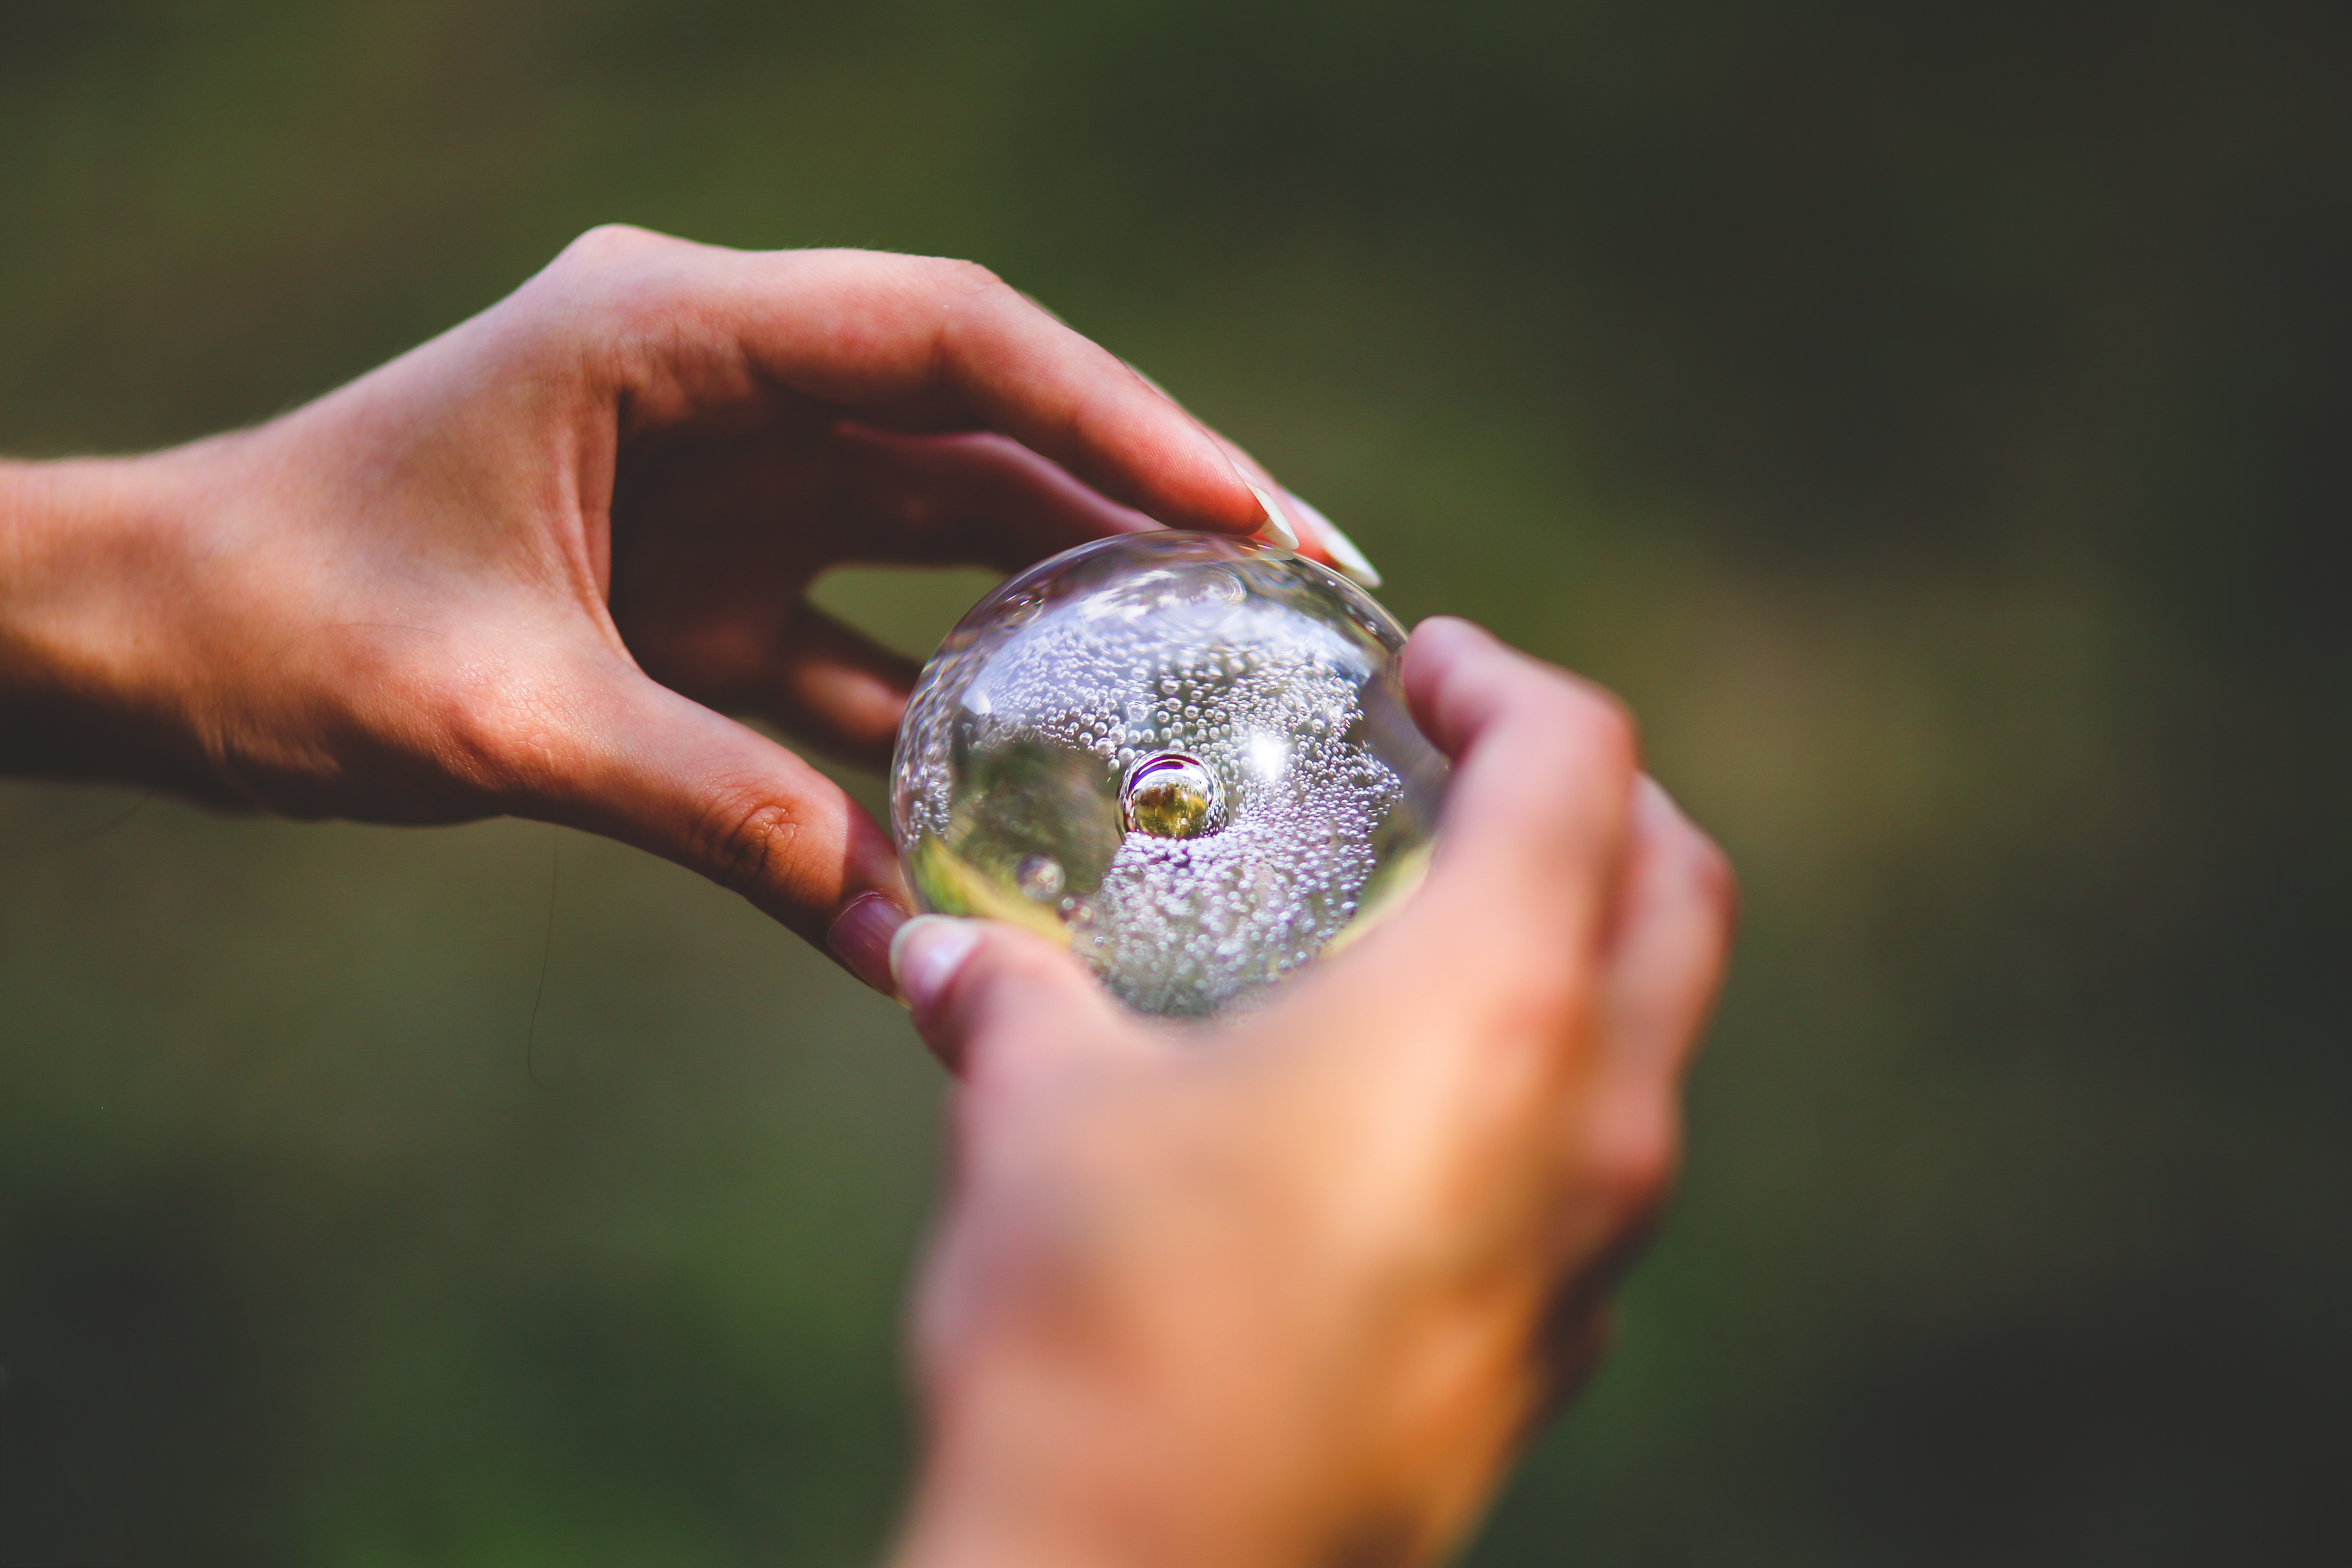
\includegraphics[width=\paperwidth]{../img/crystal.jpg}}
\end{frame}
}
\fi

\Subsection{Hantera saknade värden med \texttt{Option}}

\begin{Slide}{Hur hantera saknade värden?}\SlideFontSmall
Olika sätt att hantera saknade värden:
\begin{itemize}
\item Hitta på ett specialvärde: exempel -1 för saknat värde
\item \code{null} om värde saknas (vanligt i Java m.fl. språk, mkt ovanligt i Scala)
\item Använd en samling och låt tom samling representera saknat värde: \\
\code{val sums = Vector(Vector(42),Vector(32),Vector(),Vector(21))}

\item \code{Option[A]} gemensam bastyp för: \\
  \code{None} som representerar \Alert{saknat värde}, och \\ \code{Some[A]} som representerar att \Emph{värde finns}
\end{itemize}
\end{Slide}



\begin{Slide}{En gemensam bastyp för ett värde som kanske saknas}\SlideFontSmall\ifkompendium\footnotesize\fi
\vspace{-0.0em}\begin{center}
\newcommand{\TextBox}[1]{\raisebox{0pt}[1em][0.5em]{#1}}
\tikzstyle{umlclass}=[rectangle, draw=black,  thick, anchor=north, text width=3cm, rectangle split, rectangle split parts = 3]
\begin{tikzpicture}[inner sep=0.5em]
\node [umlclass, rectangle split parts = 2, xshift=0cm, text width=3.5cm] (BaseType)  {
            \textit{\textbf{\centerline{\TextBox{\code{Option[A]}}}}}
            \nodepart[]{second}
            \TextBox{\code{def get: A}}\newline
            \TextBox{\code{def isEmpty: Boolean}}

        };

\node [umlclass, rectangle split parts = 1]  at (-2.5cm,-3.0cm) (SubType1) {
            \textbf{\centerline{\TextBox{\code{Some[A]}}}}
            % \nodepart[]{second} \TextBox{\code{val x: A}}
        };

\node [umlclass, rectangle split parts = 1] at (2.5cm,-3.0cm) (SubType2)  {
            \textbf{\centerline{\TextBox{\code{None}}}}
        };
\draw[umlarrow] (SubType1.north) -- ++(0,0.5) -| (BaseType.south);
\draw[umlarrow] (SubType2.north) -- ++(0,0.5) -| (BaseType.south);
\end{tikzpicture}
\end{center}
\pause
\vspace{-0.5em}\begin{REPL}
scala> var x: Option[Int] = Some(42)

scala> x.isEmpty
val res0: Boolean = false

scala> x = None

scala> x.isEmpty
val res1: Boolean = true
\end{REPL}
\end{Slide}


\begin{Slide}{Option för hantering av ev. saknade värden}\SlideFontSmall
Alla vill inte berätta för Facebook vad de har för kön. \\ Förbättra Facebooks kod med ett litet Scala-program:
\begin{Code}
enum Gender:
  case Male, Female

case class Person(name: String, gender: Option[Gender])
\end{Code}
\pause
\begin{REPL}
scala> val p1 = Person("Björn",  Some(Gender.Male))
scala> val p2 = Person("Sandra", Some(Gender.Female))
scala> val p3 = Person("Kim",  None)
scala> val g2 = p2.gender
scala> def show(g: Option[Gender]): String = g match {
         case Some(x) => x.toString
         case None    => "unknown"
       }
scala> show(g2)
scala> show(p3.gender)
scala> val ps = Vector(p1,p2,p3)
scala> ps.map(_.gender).map(show)   // None ignoreras av map
\end{REPL}
\end{Slide}

\begin{Slide}{Några smidiga metoder på \code{Option}}\SlideFontSmall
Metoden \code{getOrElse} gör att man ofta kan undvika matchning.
\begin{Code}
var opt: Option[Int] = None

val x = opt.getOrElse(42)      // get the value or give a default if missing
\end{Code}

Flera av de vanliga samlingsmetoderna funkar, t.ex. \code{foreach} och \code{map}.
\begin{Code}
opt.foreach{x => println(x)}    // only done if value exists

opt.map{x => x + 1}             // only done if value exists

opt = Some(42)                  // change opt to now have some value

opt.foreach{x => println(x)}    // done as value now exists

opt.map{x => x + 1}             // done as value now exists

\end{Code}
\end{Slide}


\begin{Slide}{Några samlingsmetoder som ger en \code{Option}, övning}
\begin{REPL}
scala> val (xs, ys) = (Vector(1,2,3), Vector())

scala> xs.headOption
res0: ???

scala> ys.headOption
res1: ???

scala> xs.find(_ > 1)
res2: ???

scala> xs.find(_ > 5)
res3: ???

scala> val huvudstad = Map("Sverige" -> "Sthlm", "Skåne" -> "Malmö")

scala> huvudstad.get("Skåne")
res4: ???

scala> huvudstad.get("Danmark")
res5: ???
\end{REPL}
\end{Slide}

\begin{Slide}{Några samlingsmetoder som ger en \code{Option}, svar}
\begin{REPL}
scala> val (xs, ys) = (Vector(1,2,3), Vector())

scala> xs.headOption
res0: Option[Int] = Some(1)

scala> ys.headOption
res1: Option[Nothing] = None

scala> xs.find(_ > 1)
res2: Option[Int] = Some(2)

scala> xs.find(_ > 5)
res3: Option[Int] = None

scala> val huvudstad = Map("Sverige" -> "Sthlm", "Skåne" -> "Malmö")

scala> huvudstad.get("Skåne")
res4: Option[String] = Some(Malmö)

scala> huvudstad.get("Danmark")
res5: Option[String] = None
\end{REPL}
\end{Slide}

%!TEX encoding = UTF-8 Unicode
%!TEX root = ../lect-w06.tex

%%%



\Subsection{Undantag}

\ifkompendium\else
\begin{SlideExtra}{Undantag kan orsaka krasch...}
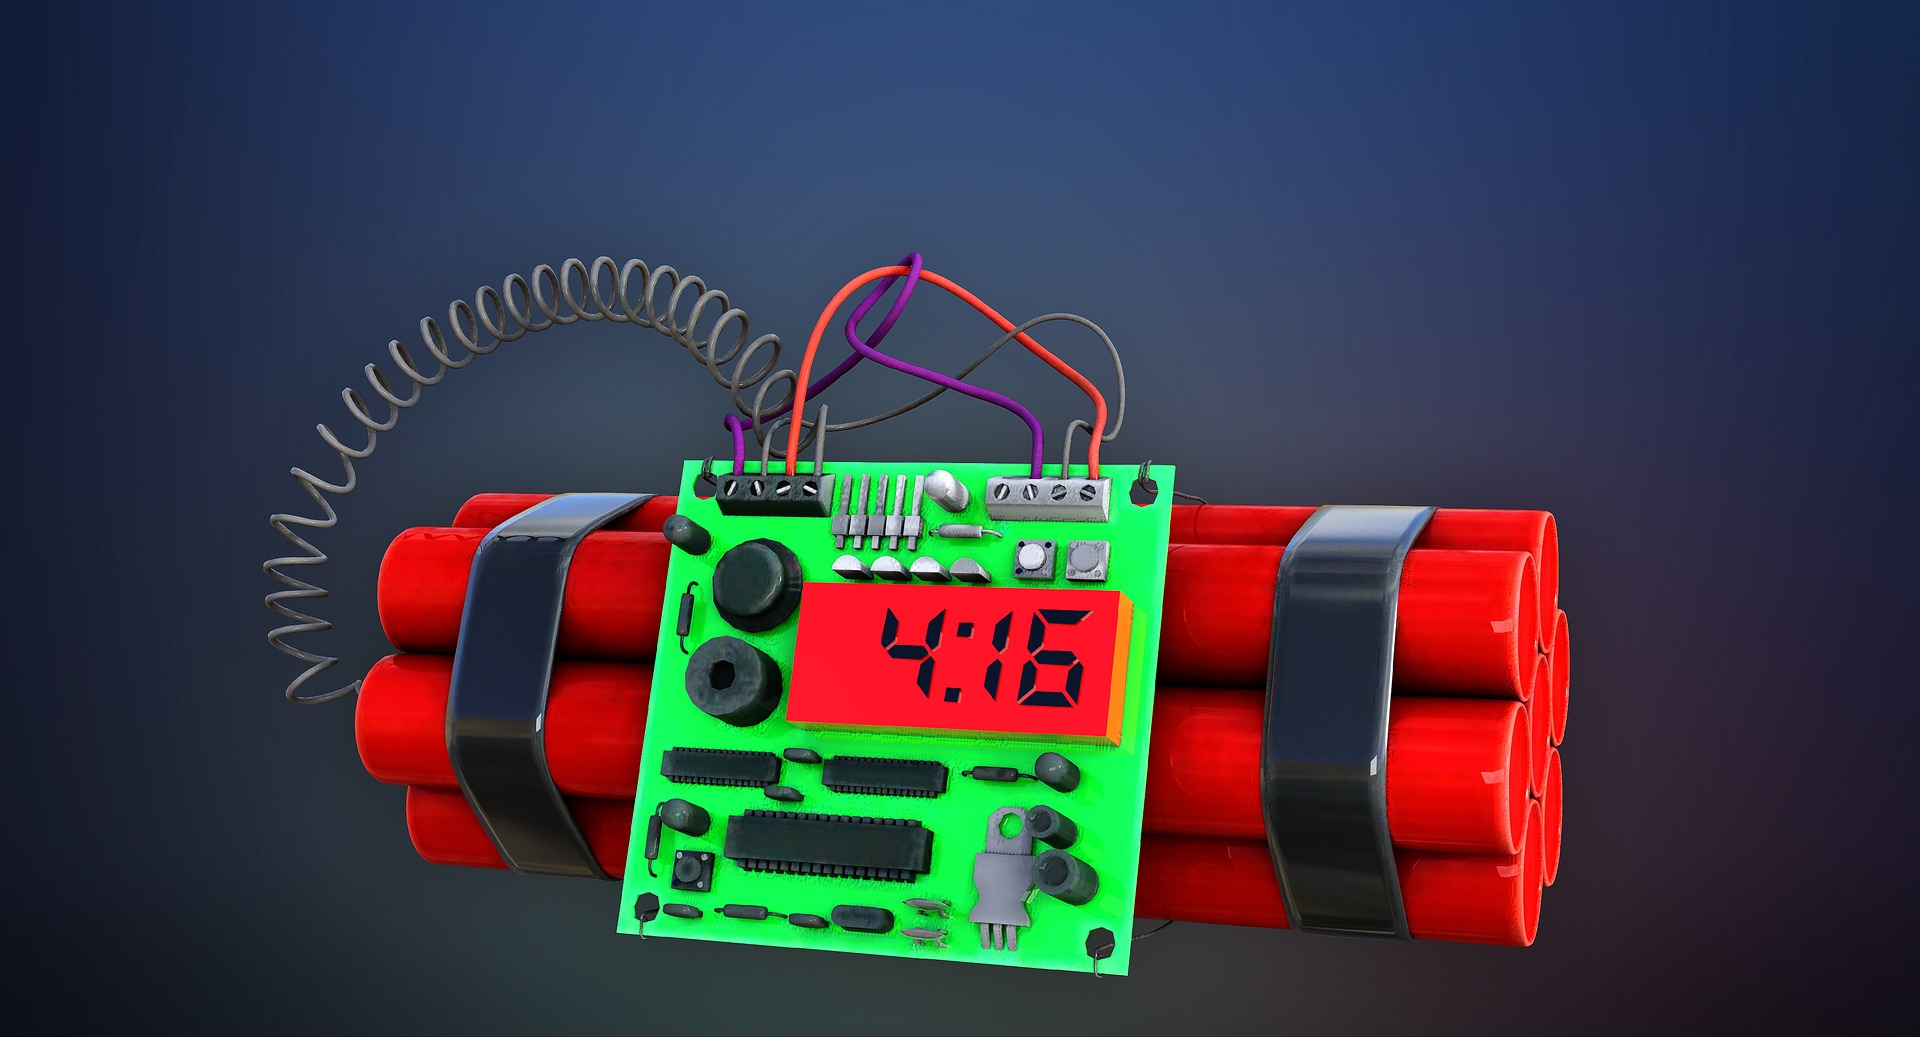
\includegraphics[width=1.0\textwidth]{../img/dynamite}  
\end{SlideExtra}

\begin{SlideExtra}{Undantag orsakar ingen krasch om inkapslad i en Try}
\hspace{0.3\textwidth}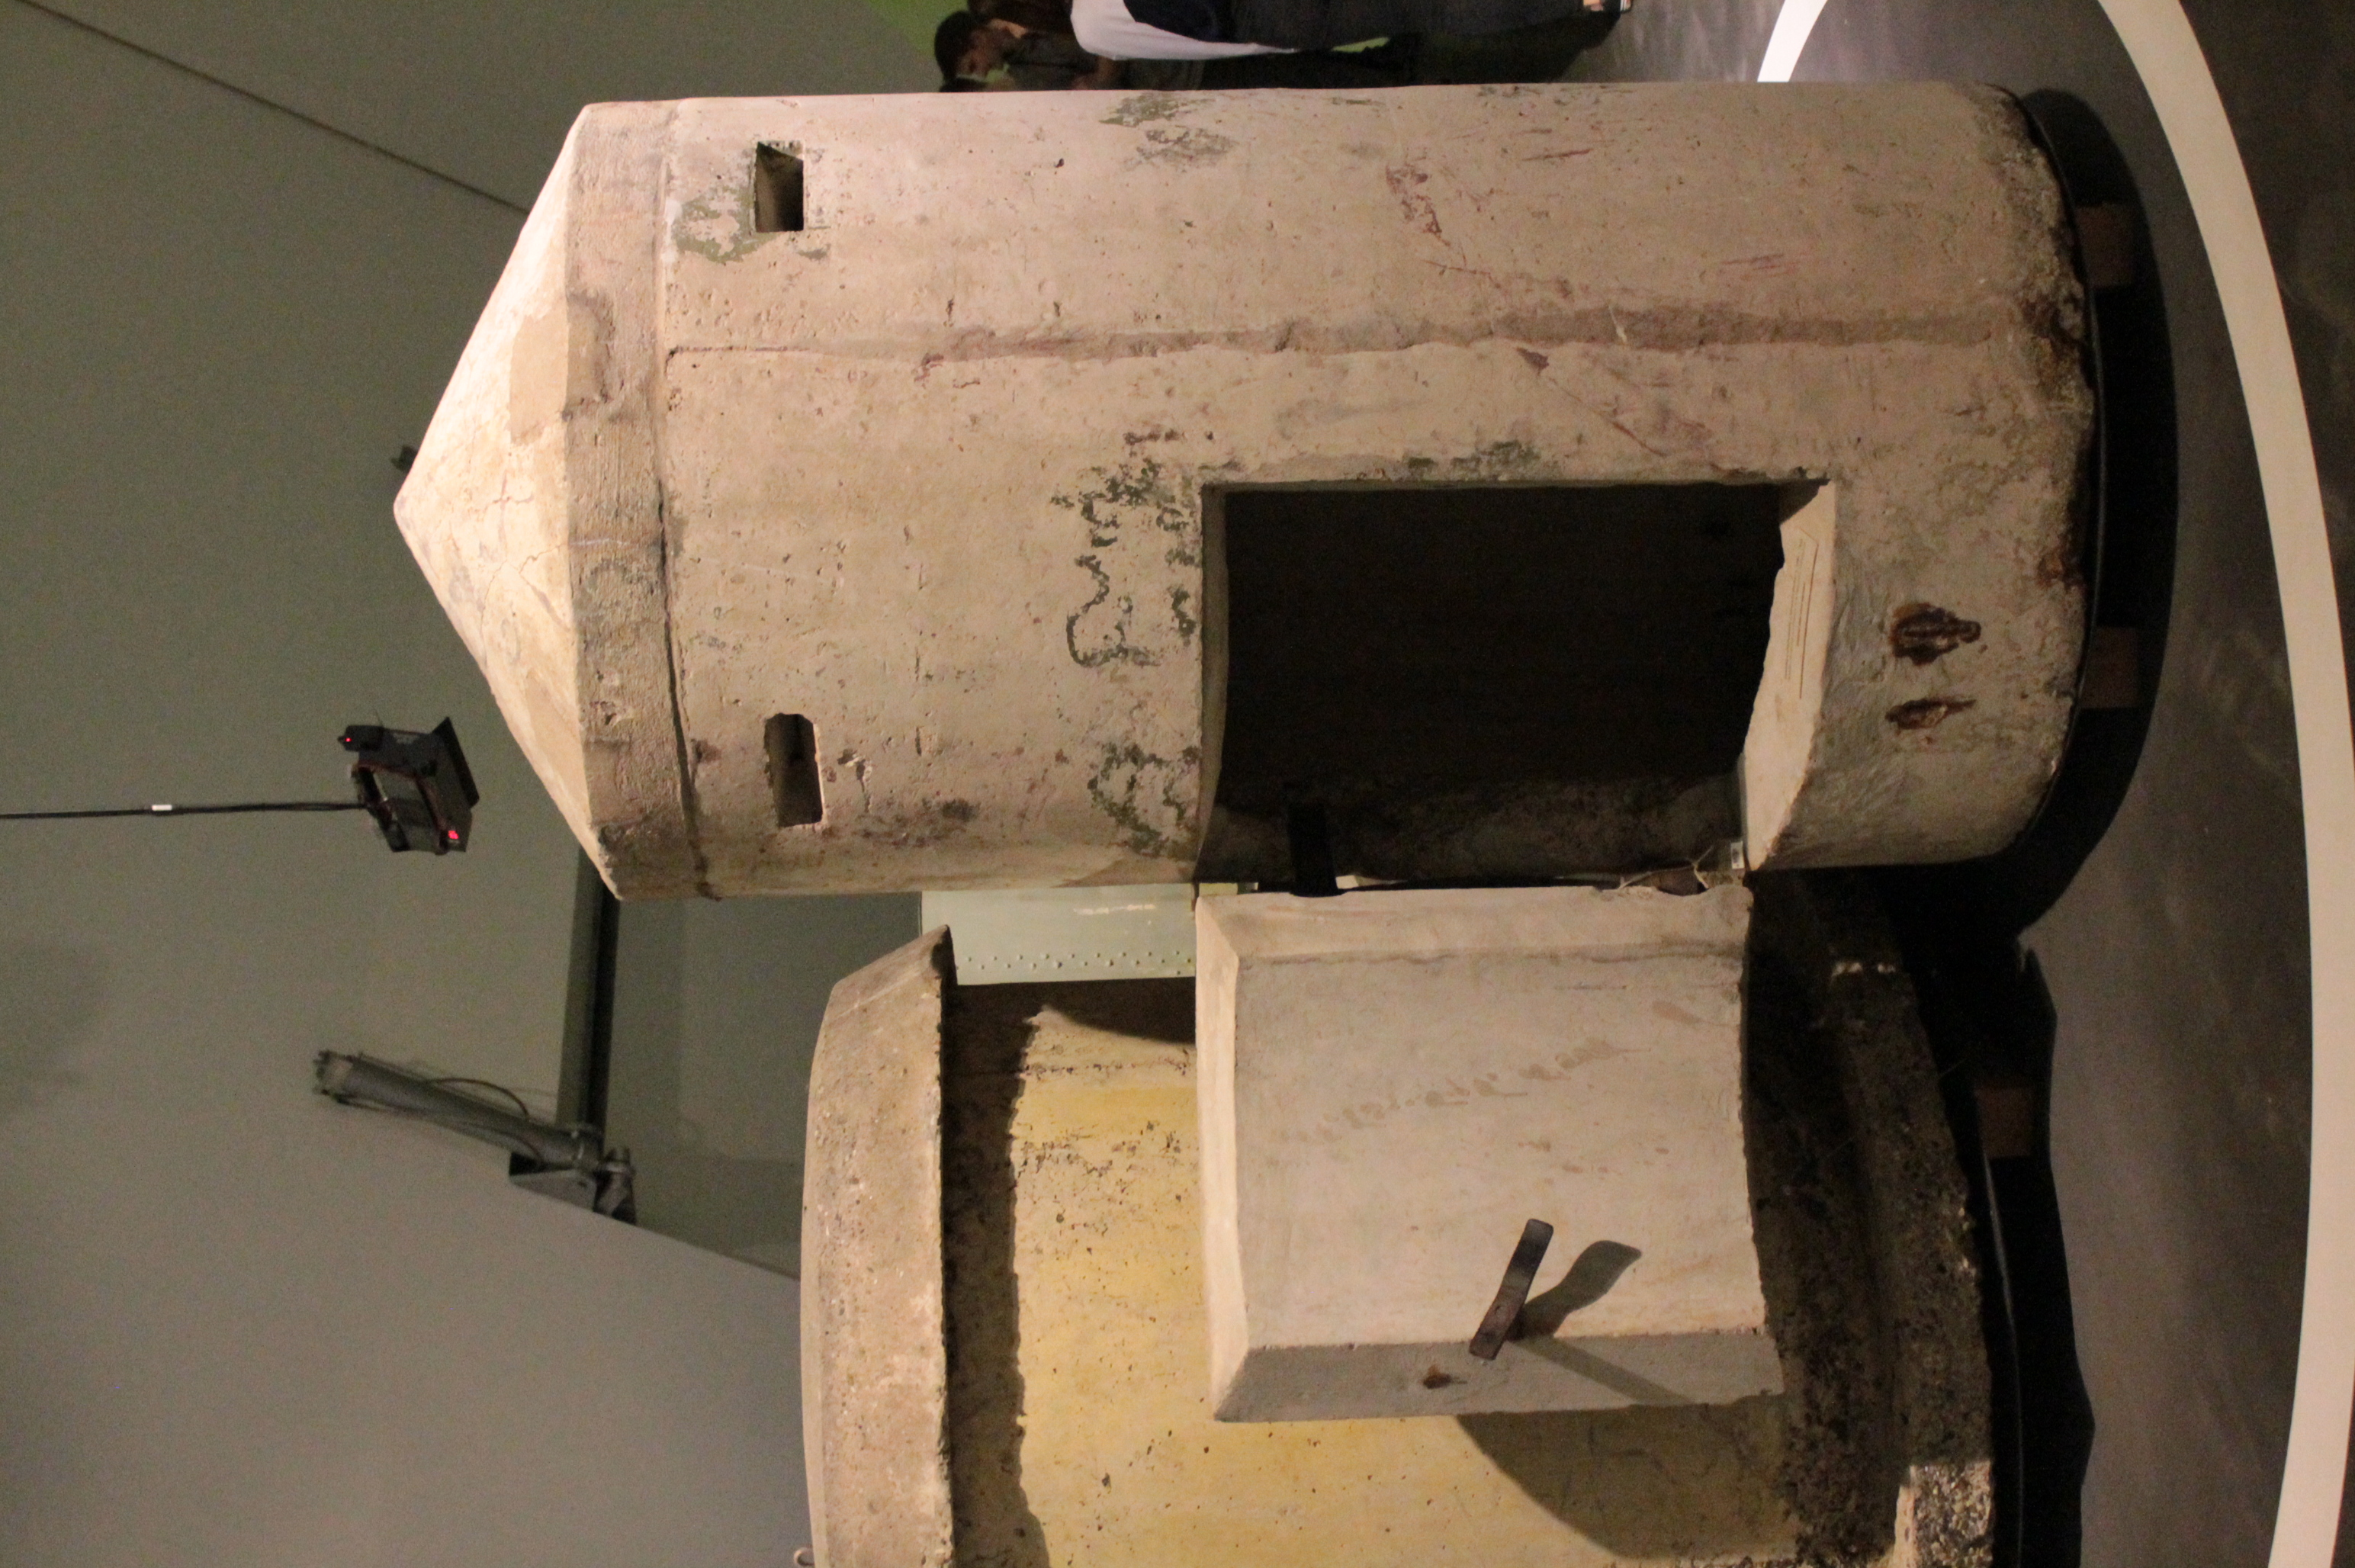
\includegraphics[width=0.6\textwidth,angle=-90,origin=c]{../img/bomb-shelter}  
\end{SlideExtra}
\fi

\begin{Slide}{Vad är ett undantag \Eng{exception}?}
Undantag representerar ett fel eller ett onormalt tillstånd som upptäcks under exekvering och som  behöver hanteras på särskilt sätt vid sidan av det normala exekveringsflödet.

\vspace{1em}\href{https://sv.wikipedia.org/wiki/Undantagshantering}{sv.wikipedia.org/wiki/Undantagshantering}


\vspace{1em} Exempel på undantag:

\pause

\begin{itemize} \SlideFontSmall
\item Indexering utanför vektorns indexgränser.

\item Läsning bortom filens slut.

\item Försök att öppna en fil som inte finns.

\item Minnet är slut.

\item Heltalsdivision med noll ger \code{java.lang.ArithmeticException}.

\item \code{"hej".toInt} ger \code{java.lang.NumberFormatException}

\end{itemize}

\end{Slide}


\begin{Slide}{Orsaka undantag indirekt med \texttt{require} och \texttt{assert}}

\begin{itemize}\SlideFontSmall
  \item Med funktionen \code{require(p)} skapas ett \\\code{IllegalArgumentException("requirement failed")} \\ om \code{p} är \code{false}
  \item \code{require} används om man vill begränsa vilka argument som är giltiga
  \item Med funktionen \code{assert(p)} skapas ett \code{AssertionError("assertion failed")} \\ om \code{p} är \code{false} 
  \item \code{assert} används om man vill förhindra ogiltiga tillstånd
\end{itemize}
{
  \ifkompendium\else
  \vfill\SlideFontTiny
  \fi
  Se implementationen av \code{require} här:\\
\url{https://github.com/scala/scala/blob/v2.13.6/src/library/scala/Predef.scala#L315}
}
\end{Slide}

\begin{Slide}{Kasta dina egna undantag med \texttt{throw}}\SlideFontSmall
Man kan själv generera ett undantag med \code{throw}, vilket kallas att \Emph{kasta} ett undantag som (om det inte \Emph{fångas}), gör att exekveringen \Alert{avbryts}.


\begin{REPL}
scala> def pang = throw Exception("PANG!")
pang: Nothing

scala> pang
java.lang.Exception: PANG!

\end{REPL}
\pause
Olika sätt att hantera undantag och förhindra att exekveringen avbryts:
\begin{itemize}
\item \code{try catch}-uttryck omvandlar undantag till ngt lämpligt värde.
%\item Java: Man kan använda en \code{try ... catch}-sats och \Alert{göra något} i händelse av undantag.

\item \texttt{scala.util.Try} \Emph{kapslar in} kod som kan ge undantag.  %(Finns ej i Java; att föredra i Scala.)
\end{itemize}
\end{Slide}


\Subsection{Hantera undantag med \texttt{Try}}

\begin{Slide}{En gemensam bastyp för något som kan misslyckas}\SlideFontSmall
\begin{Code}
import scala.util.{Try, Success, Failure}
\end{Code}
\ifkompendium\footnotesize\fi
\vspace{-0.5em}\begin{center}
\newcommand{\TextBox}[1]{\raisebox{0pt}[1em][0.5em]{#1}}
\tikzstyle{umlclass}=[rectangle, draw=black,  thick, anchor=north, text width=3.0cm, rectangle split, rectangle split parts = 3]
\begin{tikzpicture}[inner sep=0.5em]
\node [umlclass, rectangle split parts = 2, xshift=0cm, text width=3.8cm] (BaseType)  {
            \textit{\textbf{\centerline{\TextBox{\code{Try[T]}}}}}
            \nodepart[]{second}
            \TextBox{\code{def get: T}}\newline
            \TextBox{\code{def isFailure: Boolean}}\newline
            \TextBox{\code{def isSuccess: Boolean}}
        };

\node [umlclass, rectangle split parts = 2, text width=2.2cm]  at (-2.5cm,-3.7cm) (SubType1) {
            \textbf{\centerline{\TextBox{\code{Success[T]}}}}
            \nodepart[]{second} \TextBox{\code{val value: T}}
        };

\node [umlclass, rectangle split parts = 2, text width=4.2cm] at (2.5cm,-3.7cm) (SubType2)  {
            \textbf{\centerline{\TextBox{\code{Failure[T]}}}}
            \nodepart[]{second} \TextBox{\code{val exception: Throwable}}
        };
\draw[umlarrow] (SubType1.north) -- ++(0,0.5) -| (BaseType.south);
\draw[umlarrow] (SubType2.north) -- ++(0,0.5) -| (BaseType.south);
\end{tikzpicture}
\end{center}
\end{Slide}

\begin{Slide}{Hantera undantag med \texttt{Try}}
\vspace{-0.5em}\begin{REPLsmall}
scala> def pang = throw new Exception("PANG!")

scala> def kanskePang = if math.random() < 0.5 then 42 else pang

scala> import scala.util.{Try, Success, Failure}

scala> def försök = Try { kanskePang }

scala> val xs = Vector.fill(15){försök}

scala> val trettonde = xs(12) match
         case Success(value) => value
         case Failure(e) => println(e); -1

scala> (xs(12).isSuccess, xs(12).isFailure) 

scala> xs(12).getOrElse(0)

scala> xs(12).toOption

scala> försök.foreach(println)

scala> försök.map(_ + 1)

scala> for Success(x) <- xs yield x
\end{REPLsmall}
\end{Slide}

\Subsection{Hantera undantag med \texttt{try}-\texttt{catch}}


\begin{Slide}{\texttt{try}-\texttt{catch}-uttryck}\SlideFontSmall
Man kan fånga undantag med ett \code{try ... catch}-uttryck:
\begin{Code}
def carola = 
  try 
    if math.random() > 0.5 then throw Exception("stormvind")
    42
  catch 
    case e: Exception =>
      println("Fångad av en " + e.getMessage)
      -1

\end{Code}
\pause
\begin{REPL}
scala> Vector.fill(5)(carola)
Fångad av en stormvind
Fångad av en stormvind
Fångad av en stormvind
val res0: Vector[Int] = Vector(-1, 42, 42, -1, -1)
\end{REPL}
%Gör uppg. 9-11 i övn. \code{patterns} som visar hur man fångar undantag i Scala och Java. 
%Mer om undantag i fortsättningskursen.
\end{Slide}

%!TEX encoding = UTF-8 Unicode
%!TEX root = ../lect-w06.tex

%%%

\Subsection{Fördjupning: Implementera \texttt{equals}}

\ifkompendium
\noindent När du jämför värden med \code{==} anropas metoden \code{equals} som finns för alla typer. Du kan i dina egna klasser överskugga \code{equals} med en din egna definition av vad likhet ska innebära. Då är det lämpligt att använda matchning. Det är dock ett ganska omfattande arbete att implementera en korrekt likhetsjämförelse som fungerar under alla omständigheter. Ett recept för en fullständig implementation av \code{equals} ges i fördjupningen nedan. 
\fi

\begin{Slide}{Fördjupning: Implementera \texttt{equals} med \texttt{match}}
Det visar sig att \Emph{innehållslikhet} är \Alert{förvånansvärt komplicerat} att implementera, speciellt  i samband med arv.
\begin{itemize}\SlideFontSmall
\item Det enklare fallet: Gör fördjupningsuppgift \textit{''Metoden \code{equals}''} och implementera \code{equals} för innehållslikhet utan arv. \\ En bra träning på att använda \code{match}!

\item Svårare: Gör fördjupningsuppgifterna  \textit{''Överskugga \code{equals}''} och \textit{''Överskugga equals vid arv''} om du vill se hur en \Emph{komplett} \code{equals} ska se ut som fungerar \Alert{i alla lägen}.

\end{itemize}

\noindent Det krävs i denna kurs inte att du själv ska kunna implementera en generellt fungerande \code{equals}. Men du ska förstå skillnaden mellan referenslikhet och innehållslikhet. Mer om \code{equals} i fortsättningkursen, men en liten inblick i problemet nu...
\end{Slide}

\ifkompendium
\noindent Om en klass markeras \code{final} kan den ej ha några subklasser. Kompilatorn kontrollerar att detta gäller alla finala klasser och ger kompileringsfel om du försöker göra \code{extends} på en final klass. Om en klass garanterat inte har några subklasser kan implementationen av \code{equals} göra enklare.
\fi 

\begin{Slide}{Fördjupning: \texttt{equals} som fungerar för finala klasser}
Recept för implementation av \code{equals} som fungerar för typer som \Alert{inte} har några subtyper:
\begin{Code}
final class Gurka(val vikt: Int, val ärÄtbar: Boolean):
  override def equals(other: Any): Boolean = other match
    case that: Gurka => vikt == that.vikt && ärÄtbar == that.ärÄtbar
    case _ => false

  override def hashCode: Int = (vikt, ärÄtbar).## // ger bra hashcode
\end{Code}
\begin{itemize}\SlideFontSmall
\item
Du \Alert{måste} alltid överskugga \code{hashCode} också om du överskuggar \code{equals} annars funkar inte gurksamlingar (lång story ...)
\item
Notera typen \code{Any} -- detta följer hur man valde att göra i Java (tyvärr?).
\pause
\item
Ett \Alert{typsäkrare} innehållslikhetstest som \Emph{garanterat} bara jämför en gurka med en gurka och inget annat:
\begin{Code}
def ===(other: Gurka): Boolean =
  vikt == other.vikt && ärÄtbar == other.ärÄtbar
\end{Code}
\end{itemize}
\end{Slide}


\begin{Slide}{Fördjupning: Recept i 8 steg för arvssäker \code{equals}}\SlideFontTiny
%fungerar även för klasser som inte är \code{final}:
\SlideOnly{\setlength{\leftmargini}{0pt}}
\begin{enumerate}\SlideFontTiny
\item Inför denna metod: \code{ def canEqual(other: Any): Boolean}\\Observera att typen på parametern ska vara \code{Any}. Om subklass behövs \code{override}.

\item Metoden \code{canEqual} ska ge \code{true} om \code{other} är av samma typ som \code{this}, t.ex.: \\\code{override def canEqual(other: Any): Boolean = other.isInstanceOf[Gurka]}

\item Inför metoden \code{equals} och var noga med att parametern har typen \code{Any}: \\ \code{override def equals(other: Any): Boolean}

\item Implementera metoden \code{equals} med ett match-uttryck som börjar så här: \\
\code|other match { ... } |

\item Match-uttrycket ska ha två grenar. Den första grenen ska ha ett typat mönster för den klass som ska jämföras, t.ex.: \\ \code{  case that: Gurka =>}

\item Om du implementerar \code{equals} i den klass som inför \code{canEqual}, börja med: \\ \code{(that canEqual this) &&} \\
och skapa därefter en fortsättning som baseras på innehållet i klassen, t.ex.: \\ \code{this.vikt == that.vikt && this.längd == that.längd} \\
Om du överskuggar equals vill du nog börja med
 \code{super.equals(that) && }

\item Den andra grenen i matchningen ska vara:
\code{case _ => false}

\item Överskugga \code{hashCode}, t.ex. med tupel av attributvärden och metoden \code{##}: \\
\code{override def hashCode: Int  = (vikt, längd).## }

\end{enumerate}
\url{http://www.artima.com/pins1ed/object-equality.html}

\end{Slide}


\begin{Slide}{Fördjupning: Säkrare likhetstest i Scala 3}
\SlideFontSmall
\begin{itemize}
\item \Alert{Problem}: \code{equals} tar värden av vilken typ som helst.
\item Detta kallas \Alert{universell likhet}.
\item[]
\begin{REPLsmall}
scala> case class Hund(namn: String)
scala> case class Katt(namn: String)
scala> Hund("bob") == Katt("bob") // knasig jämförelse; kan aldrig bli sant
val res0: Boolean = false         // men kompilatorn låter dig göra likhetstestet
\end{REPLsmall}  
\item I Scala 3 kan du få typsäker likhetstest med~~\code{derives CanEqual}
\item Detta kalla \Emph{multiversell likhet}.
\item[]
\begin{REPLsmall}
scala> case class Hund(namn: String) derives CanEqual
scala> Hund("bob") == Katt("bob")   // tack kompilatorn för fel:
-- Error:
1 |Hund("bob") == Katt("bob")
  |^^^^^^^^^^^^^^^^^^^^^^^^^^
  |Values of types Hund and Katt cannot be compared with == or !=
\end{REPLsmall}  
\item Du \Emph{slipper} skriva \code{derives CanEqual} om du gör: \\ \code{import scala.language.strictEquality}
\item Läs mer här: \url{https://docs.scala-lang.org/scala3/reference/contextual/multiversal-equality.html}

\end{itemize}

\end{Slide}



%!TEX encoding = UTF-8 Unicode
%!TEX root = ../exercises.tex

\ifPreSolution



\Exercise{\ExeWeekSIX}\label{exe:W06}

\begin{Goals}
\item Kunna skapa och använda \code{match}-uttryck med konstanta värden, garder och mönstermatchning med case-klasser.
\item Kunna skapa och använda case-objekt för matchningar på uppräknade värden.
\item Kunna hantera saknade värden med hjälp av typen \code{Option} och mönstermatchning på \code{Some} och \code{None}.
\item Kunna fånga undantag med \code{scala.util.Try}.
\item Känna till \code{try}, \code{catch} och \code{throw}.
%\item Känna till \jcode{switch}-satser i Java.
\item Känna till nyckelordet \code{sealed} och förstå nyttan med förseglade typer.
%\item Känna till relationen mellan \code{hashCode} och \code{equals}.
%\item Kunna skapa partiella funktioner med case-uttryck.
%\item Känna till betydelsen av små och stora begynnelsebokstäver i case-grenar i en matchning, samt förstå hur namn binds till värden in en case-gren.
%\item Kunna använda \code{flatMap} tillsammans med \code{Option} och \code{Try}.
%\item Känna till skillnaderna mellan \code{try}-\code{catch} i Scala och java.
\item Känna till att metoden \code{unapply} används vid mönstermatchning.
%\item Kunna implementera \code{equals} med hjälp av en \code{match}-sats, som fungerar för finala klasser utan arv.
%\item Känna till \code{null}.
\end{Goals}

\begin{Preparations}
\item \StudyTheory{06}
\end{Preparations}

\BasicTasks %%%%%%%%%%%%%%%%

\else



\ExerciseSolution{\ExeWeekSIX}

\BasicTasks %%%%%%%%%%%

\fi





% \WHAT{Hur fungerar en \jcode{switch}-sats i Java (och flera andra språk)?}

% \QUESTBEGIN

% \Task \label{task:switch} \what~   Det händer ofta att man vill testa om ett värde är ett av många olika alternativ. Då kan man använda en sekvens av många \code{if}-\code{else}, ett för varje alternativ. Men det finns ett annat sätt i Java och många andra språk: man kan använda \jcode{switch} som kollar flera alternativ i en och samma sats, se t.ex. \href{https://en.wikipedia.org/wiki/Switch_statement}{en.wikipedia.org/wiki/Switch\_statement}.

% \Subtask Skriv in nedan kod i en kodeditor. Spara med namnet \texttt{Switch.java} och kompilera filen med kommandot \texttt{javac Switch.java}. Kör den med \texttt{java Switch} och ange din favoritgrönsak som argument till programmet. Vad händer? Förklara hur \jcode{switch}-satsen fungerar.

% \javainputlisting[numbers=left,basicstyle=\ttfamily\fontsize{9}{11}\selectfont]{examples/Switch.java}

% \Subtask \label{subtask:break} Vad händer om du tar bort \jcode{break}-satsen på rad 16?




% \SOLUTION


% \TaskSolved \what


% \SubtaskSolved  Beroende på första bokstaven i din favoritgrönsak får du olika svar såsom \textit{gurka är gott!} vid första bokstaven $g$.\\
% Javas \jcode{switch}-sats testar den första bokstaven på favoritgrönsaken genom att stegvis jämföra den med \jcode{case}-uttrycken. Om första bokstaven \jcode{firstChar} matchar bokstaven efter ett \jcode{case} körs koden efter kolonet till \jcode{switch}-satsens slut eller tills ett \jcode{break} avbryter \jcode{switch}-satsen.\\
% Matchar inte \jcode{firstChar} något \jcode{case} så finns även \jcode{default}, som körs oavsett vilken första bokstaven är, ett generellt fall.

% \SubtaskSolved  Om \jcode{case 't'} körs kommer både  \textit{tomat är gott!} och \textit{broccoli är gott!} skrivas ut, man säger att koden $"$faller igenom$"$. Utan \jcode{break}-satsen i Java körs koden i efterkommande \jcode{case} tills ett \jcode{break} avbryter exekveringen eller \jcode{switch}-satsen tar slut.



% \QUESTEND






\WHAT{Matcha på konstanta värden.}

\QUESTBEGIN

\Task \label{task:vegomatch} \what~   % I Scala finns ingen \jcode{switch}-sats. I stället har Scala ett \code{match}-uttryck som är mer kraftfullt. Dock saknar Scala nyckelordet \jcode{break} och Scalas \code{match}-uttryck kan inte ''falla igenom'' som skedde i uppgift \ref{task:switch}\ref{subtask:break}.

\Subtask \label{subtask:vegomatch} Skriv nedan program med en kodeditor och spara i filen \texttt{Match.scala}. Kompilera med \texttt{scalac Match.scala}. Kör med \texttt{scala Match} och ge som argument din favoritgrönsak. Vad händer? Förklara hur ett \code{match}-uttryck fungerar.

\scalainputlisting[numbers=left,basicstyle=\ttfamily\fontsize{11}{12}\selectfont]{examples/Match.scala}

\Subtask Vad blir det för felmeddelande om du tar bort case-grenen för defaultvärden och indata väljs så att inga case-grenar matchar? Är det ett exekveringsfel eller ett kompileringsfel?

% \Subtask Beskriv några skillnader i syntax och semantik mellan Javas flervalssats \jcode{switch} och Scalas flervalsuttryck \code{match}.



\SOLUTION


\TaskSolved \what


\SubtaskSolved  Svaret blir identiskt mot föregående uppgiften i Java.\\
Scalas \code{match}-uttryck fungerar väldigt likt Javas \jcode{switch}. Den jämför stegvis värdet med varje \code{case} för att sedan returnera ett värde tillhörande motsvarande \code{case}.

\SubtaskSolved  \begin{REPL}
scala.MatchError (of class java.lang.Character)
\end{REPL}
Exekveringsfel, uppstår av en viss input under körningen.

% \SubtaskSolved  Scalas \code{match} ersätter kolonet (:) i \jcode{switch} med Scalas högerpil (=>).\\
% \code{match} returnerar ett värde till skillnad från \jcode{switch} som inte returnerar något.\\
% \code{match} kan inte $"$falla igenom$"$ så ett \jcode{break} efter varje \jcode{case} är inte nödvändigt.\\
% Till skillnad från \jcode{switch}-satsen kastar \code{match} ett \code{MatchError} om ingen matchning skulle ske.



\QUESTEND






\WHAT{Gard i case-grenar.}

\QUESTBEGIN

\Task  \what~  Med hjälp en gard \Eng{guard} i en case-gren kan man begränsa med ett villkor om grenen ska väljas.

Utgå från koden i uppgift \ref{task:vegomatch}\ref{subtask:vegomatch} och byt ut case-grenen för \code{'g'}-matchning till nedan variant med en gard med nyckelordet \code{if} (notera att det inte behövs parenteser runt villkoret):
\begin{Code}
    case 'g' if math.random() > 0.5 => "gurka är gott ibland..."
\end{Code}
Kompilera om och kör programmet upprepade gånger med olika indata tills alla grenar i \code{match}-uttrycket har exekverats. Förklara vad som händer.

\SOLUTION


\TaskSolved \what

Garden som införts vid \code{case 'g'} slumpar fram ett tal mellan 0 och 1 och om talet inte är större än $0.5$ så blir det ingen matchning med \code{case 'g'} och programmet testar vidare tills default-caset.\\
Gardens krav måste uppfyllas för att det ska matcha som vanligt.



\QUESTEND






\WHAT{Mönstermatcha på attributen i case-klasser.}

\QUESTBEGIN

\Task \label{task:match-caseclass} \what~   Scalas \code{match}-uttryck är extra kraftfulla om de används tillsammans med \code{case}-klasser: då kan attribut extraheras automatiskt och bindas till lokala variabler direkt i case-grenen som nedan exempel visar (notera att \code{v} och \code{rutten} inte behöver deklareras explicit). Detta kallas för \textbf{mönstermatchning}.

\Subtask \label{subtask:autobinding-match} Vad skrivs ut nedan? Varför? Prova att byta namn på \code{v} och \code{rutten}.
\begin{REPL}
scala> case class Gurka(vikt: Int, ärRutten: Boolean)
scala> val g = Gurka(100, true)
scala> g match { case Gurka(v,rutten) => println("G" + v + rutten) }
\end{REPL}

%\TODO Tab två gånger fungerar inte i scala3-repl
\Subtask Skriv sedan nedan i REPL och tryck TAB två gånger efter punkten. Vad har \code{unapply}-metoden för resultattyp?
\begin{REPL}
scala> Gurka.unapply   // Tryck TAB två gånger
\end{REPL}
\begin{Background}
Case-klasser får av kompilatorn automatiskt ett kompanjonsobjekt \Eng{companion object}, i detta fallet \code{object Gurka}. Det objektet får av kompilatorn automatiskt en \code{unapply}-metod. Det är \code{unapply} som anropas ''under huven'' när case-klassernas attribut extraheras vid mönstermatchning, men detta sker alltså automatiskt och man behöver inte explicit nyttja \code{unapply} om man inte själv vill implementera s.k. extraherare \Eng{extractors}; om du är nyfiken på detta, se fördjupningsuppgift \ref{task:extractor}.
\end{Background}

\Subtask Anropa \code{unapply}-metoden enligt nedan. Vad blir resultatet?
\begin{REPL}
scala> Gurka.unapply(g)
\end{REPL}
Vi ska i senare uppgifter undersöka hur typerna \code{Option} och \code{Some} fungerar och hur man kan ha nytta av dessa i andra sammanhang.

% \Subtask Spara programmet nedan i filen \texttt{vegomatch.scala} och kompilera och kör med \code{scala vegomatch.Main 1000} i terminalen. Förklara hur predikatet \code{ärÄtvärd} fungerar.
% \scalainputlisting[numbers=left,basicstyle=\ttfamily\fontsize{11}{12}\selectfont]{examples/vegomatch.scala}
%

\SOLUTION


\TaskSolved \what


\SubtaskSolved  G100true. Vid byte av plats: Gtrue100.\\
\code{match} testar om kompanjonsobjektet \code{Gurka} är av typen \code{Gurka} med två parametervärden. De angivna parametrarna tilldelas namn, \code{vikt} får namnet \code{v} och \code{ärRutten} namnet \code{rutten} och skrivs sedan ut. Byts namnen dessa ges skrivs de ut i den omvända ordningen.

\SubtaskSolved  \code{Option[(Int, Boolean)]}
%TODO detta är inte längre fallet i scala3-repl

%\SubtaskSolved  \code{Some((100, true))}, en \code{Option} med en tupel av parametrarna från g.
\SubtaskSolved	\code{Gurka(100, true)}
%TODO eventuellt skriv mer utförligt

% \SubtaskSolved  \code{ärÄtvärd} testar om \code{Grönsak g} är av typen \code{Gurka(v, rutten)} eller \code{Tomat}. Dessa har sedan garder.\\ \code{Gurka} måste ha \code{vikt} över 100 och \code{ärRutten} vara \code{false} för att \code{case Gurka} ska returnera \code{true}.\\
% \code{Tomat} måste ha \code{vikt} över 50 och \code{ärRutten} vara \code{false} för att \code{case Tomat} ska returnera \code{true}.\\
% Matchas inte \code{Grönsak g} med någon av dessa returneras default-värdet \code{false}.



\QUESTEND







\WHAT{Matcha på case-objekt och nyttan med \code{sealed}.}

\QUESTBEGIN

\Task	\what~	Skriv nedan kodrader i en REPL en för en. Notera nyckelordet \code{sealed} som används för att försegla en typ. En \textbf{förseglad typ} måste ha alla sina subtyper i en och samma kodfil.
\begin{REPL}
scala> sealed trait Färg
scala> case object Spader extends Färg
\end{REPL}
\Subtask Hur lyder felmeddelandet och varför sker det? Är det ett kompileringsfel eller ett körtidsfel?

\Subtask  %\label{task:match-sealedtrait-caseobject}
Skapa nu nedan kod i en editor och klistra in i REPL.
\begin{Code}
object Kortlek:
  sealed trait Färg
  object Färg:
      val values = Vector(Spader, Hjärter, Ruter, Klöver)
  case object Spader extends Färg
  case object Hjärter extends Färg
  case object Ruter extends Färg
  case object Klöver extends Färg
\end{Code}

\Subtask \label{subtask:match-sealedtrait} Skapa en funktion \code{def parafärg(f: Färg): Färg} i en editor, som med hjälp av ett match-uttryck returnerar parallellfärgen till en färg. Parallellfärgen till \code{Hjärter} är \code{Ruter} och vice versa, medan parallellfärgen till \code{Klöver} är \code{Spader} och vice versa. Klistra in funktionen i REPL. Passa även på att skriva en \code{import-sats} för det yttre objektet \textbf{Kortlek}, så medlemmarna av objektet kan nås enkelt.
\begin{REPL}
scala> parafärg(Spader)
scala> val xs = Vector.fill(5)(Färg.values((math.random() * 4).toInt))
scala> xs.map(parafärg)
\end{REPL}

\Subtask Vi ska nu undersöka vad som händer om man glömmer en av case-grenarna i matchningen i \code{parafärg}. ''Glöm'' alltså avsiktligt en av case-grenarna och klistra in den nya \code{parafärg} med den ofullständiga matchningen. Hur lyder varningen? Kommer varningen vid körtid eller vid kompilering?

\Subtask Anropa \code{parafärg} med den ''glömda'' färgen. Hur lyder felmeddelandet? Är det ett kompileringsfel eller ett körtidsfel?

\Subtask Förklara vad nyckelordet \code{sealed} innebär och vilken nytta man kan ha av att \textbf{försegla} en supertyp.


\SOLUTION


\TaskSolved \what

\SubtaskSolved
%Illegal inheritance from sealed trait Färg
\begin{REPL}
Cannot extend sealed trait Färg in a different source file
\end{REPL}
Felmeddelandet fås av att REPL:en behandlar varje inmatning individuellt och tillåter därför inte att subtypen \code{Spader} förlänger \Eng{extends} supertypen \code{Färg} eftersom denna var förseglad \Eng{sealed}. Mer om detta senare i kursen...

\SubtaskSolved
-

\SubtaskSolved
\begin{Code}
def parafärg(f: Färg): Färg = f match
  case Spader  => Klöver
  case Hjärter => Ruter
  case Ruter   => Hjärter
  case Klöver  => Spader
\end{Code}

\SubtaskSolved
\begin{REPL}
<console>:17: warning: match may not be exhaustive.
It would fail on the following input: Ruter
\end{REPL}
Varningen kommer redan vid kompilering.

\SubtaskSolved
\begin{REPL}
scala.MatchError: Ruter (of class Ruter)
  at .parafärg(<console>:17)
\end{REPL}
Detta är ett körtidsfel.

\SubtaskSolved  Om en klass är \code{sealed} innebär det att om ett element ska matchas och är en subtyp av denna klass så ger Scala varning redan vid kompilering om det finns en risk för ett \code{MatchError}, alltså om \code{match}-uttrycket inte är uttömmande och det finns fall som inte täcks av ett \code{case}.\\
En förseglad supertyp innebär att programmeraren redan vid kompileringstid får en varning om ett fall inte täcks och i sånt fall vilket av undertyperna, liksom annan hjälp av kompilatorn. Detta kräver dock att alla subtyperna delar samma fil som den förseglade klassen.



\QUESTEND


%\WHAT{Mönstermatcha med nyttan av \code{enum}.}

%\QUESTBEGIN

%\Task	\what~ Vi ska nu undersöka och jämföra skillnad mellan nyckelorden \code{enum} och \code{sealed}. Skriv nedan kod i en REPL.
%\begin{Code}
%enum Färg:
%  case Spader, Hjärter, Ruter, Klöver
%\end{Code}

%\Subtask Skapa igen i en editor en funktion \code{def paraFärg(f: Färg): Färg}, nästintill likadan som den som vi skapade i deluppgift \ref{task:match-sealedtrait-caseobject} %\ref{subtask:match-sealedtrait}. Funktionen ska återigen utnyttja match-uttryck för att returnera paralellfärgen till argumentet som ges. Klistra in funktionen i REPL.
%\begin{REPL}
%scala> parafärg(Färg.Ruter)
%scala> val xs = Vector.fill(5)(Färg.values((math.random() * 4).toInt))
%scala> xs.map(parafärg)
%\end{REPL}


%\SOLUTION


%\TaskSolved \what

%\SubtaskSolved
%\begin{Code}
%def parafärg(f: Färg): Färg = f match
%  case Färg.Spader  => Färg.Klöver
%  case Färg.Hjärter => Färg.Ruter
%  case Färg.Ruter   => Färg.Hjärter
%  case Färg.Klöver  => Färg.Spader
%\end{Code}


%\QUESTEND


\WHAT{Betydelsen av små och stora begynnelsebokstäver vid matchning.}

\QUESTBEGIN

\Task  \what~  För att åstadkomma att namn kan bindas till variabler vid matchning utan att de behöver deklareras i förväg (som vi såg i uppgift \ref{task:match-caseclass}\ref{subtask:autobinding-match}) så har identifierare med liten begynnelsebokstav fått speciell betydelse: den tolkas av kompilatorn som att du vill att en variabel  binds till ett värde vid matchningen. En identifierare med stor begynnelsebokstav tolkas däremot som ett konstant värde (t.ex. ett case-objekt eller ett case-klass-mönster).

\Subtask \emph{En case-gren som fångar allt}. En case-gren med en identifierare med liten begynnelsebokstav som saknar gard kommer att matcha allt. Prova nedan i REPL, men försök lista ut i förväg vad som kommer att hända. Vad händer?
\begin{REPL}
scala> val x = "urka"
scala> x match
         case str if str.startsWith("g") => println("kanske gurka")
         case vadsomhelst => println("ej gurka: " + vadsomhelst)
scala> val g = "gurka"
scala> g match
         case str if str.startsWith("g") => println("kanske gurka")
         case vadsomhelst => println("ej gurka: " + vadsomhelst)
\end{REPL}

\Subtask \emph{Fallgrop med små begynnelsbokstäver.} Innan du provar nedan i REPL, försök gissa vad som kommer att hända. Vad händer? Hur lyder varningarna och vad innebär de?
\begin{REPL}
scala> val any: Any = "varken tomat eller gurka"
scala> case object Gurka
scala> case object tomat
scala> any match
         case Gurka => println("gurka")
         case tomat => println("tomat")
         case _ => println("allt annat")
\end{REPL}

\Subtask \emph{Använd backticks för att tvinga fram match på konstant värde.} Det finns en utväg om man inte vill att kompilatorn ska skapa en ny lokal variabel: använd specialtecknet \emph{backtick}, som skrivs \`{} och kräver speciella tangentbordstryck.\footnote{Fråga någon om du inte hittar hur man gör backtick \`{} på ditt tangentbord.}  Gör om föregående uppgift men omgärda nu identifieraren \code{tomat} i tomat-case-grenen med backticks, så här: \code{  case `tomat` => ...}



\SOLUTION


\TaskSolved \what


\SubtaskSolved  Både \code{str} och \code{vadsomhelst} matchar med inputen, oavsett vad denna är på grund av att de har en liten begynnelsebokstav.\\
 \code{str} har dock en gard att strängen måste börja med $g$ vilket gör så endast \code{val g = "gurka"} matchar med denna. \code{val x = "urka"} plockas dock upp av \code{vadsomhelst} som är utan gard.

\SubtaskSolved
\begin{REPL}
<console>:16: warning: patterns after a variable pattern cannot match (SLS 8.1
.1)
\end{REPL}
och
\begin{REPL}
<console>:17: warning: unreachable code due to variable patter 'tomat' on line
16
\end{REPL}
Trots att en klass \code{tomat} existerar så tolkar Scalas \code{match} den som en \code{case}-gren som fångar allt på grund av en liten begynnelsebokstav. Detta gör så alla objekt som inte är av typen \code{Gurka} kommer ge utskriften \textit{tomat} och att sista caset inte kan nås.

\SubtaskSolved
\begin{Code}
case `tomat` => println("tomat")
\end{Code}



\QUESTEND





\WHAT{Matcha på innehåll i en Vector.}

\QUESTBEGIN

\Task \what ~ Kör nedan i REPL. Vad skrivs ut? Förklara vad som händer.
\begin{REPL}
scala> val xss = Vector(Vector("hej"),Vector("på", "dej"),Vector("4","x","2"))
scala> xss.map( _ match
  case Vector() => "tom"
  case Vector(a) => a.reverse
  case Vector(_, b) => b.reverse
  case Seq(a, "x", b) => a + b
  case _ => "ANNARS DETTA"
  ).foreach(println)
\end{REPL}


\SOLUTION

\TaskSolved \what

\begin{REPL}
jeh
jed
42
\end{REPL}
För varje element i \code{xss} görs en matching som resulterar i en sträng. Vad som händer i varje gren förklaras nedan.
\begin{enumerate}
  \item Första match-grenen aktiveras aldrig eftersom \code{xss} ej innehåller någon tom vektor.
  \item Andra grenen passar med \code{Vector("hej")} och variablen \code{a} binds till \code{"hej"}.
  \item Tredje grenen matchar \code{Vector("på", "dej")} där första värdet binds inte till någon variabel eftersom understreck finns på motsvarande plats, medan andra värdet binds till \code{b}.
  \item Fjärde grenen matchar en sekvens med tre värden där mittenvärdet är \code{"x"}. Den sista grenen aktiveras inte i detta exempel men hade matchat allt som inte fångas av tidigare grenar.
\end{enumerate}

\QUESTEND




\WHAT{Använda \code{Option} och matcha på värden som kanske saknas.}

\QUESTBEGIN

\Task  \what~  Man behöver ofta skriva kod för att hantera värden som eventuellt saknas, t.ex. saknade telefonnummer i en persondatabas. Denna situation är så pass vanlig att många språk har speciellt stöd för saknande värden.

I Java\footnote{Scala har också \code{null} men det behövs bara vid samverkan med Java-kod.} används värdet \code{null} för att indikera att en referens saknar värde. Man får då komma ihåg att testa om värdet saknas varje gång sådana värden ska behandlas, t.ex. med \code+if (ref != null) { ...} else { ... }+. Ett annat vanligt trick är att låta \code{-1} indikera saknade positiva heltal, till exempel saknade index, som får behandlas med \code+if (i != -1) { ...} else { ... }+.

I Scala finns en speciell typ \code{Option} som möjliggör smidig och typsäker hantering av saknade värden. Om ett kanske saknat värde packas in i en \code{Option} \Eng{wrapped in an Option}, finns det i en speciell slags samling som bara kan innehålla \emph{inget} eller \emph{något} värde, och alltså har antingen storleken \code{0} eller \code{1}.

\Subtask Förklara vad som händer nedan.
\begin{REPL}
scala> var kanske: Option[Int] = None
scala> kanske.size
scala> kanske = Some(42)
scala> kanske.size
scala> kanske.isEmpty
scala> kanske.isDefined
scala> def ökaOmFinns(opt: Option[Int]): Option[Int] = opt match
         case Some(i) => Some(i + 1)
         case None    => None
scala> val annanKanske = ökaOmFinns(kanske)
scala> def öka(i: Int) = i + 1
scala> val merKanske = kanske.map(öka)
\end{REPL}

\Subtask Mönstermatchingen ovan är minst lika knölig som en \code{if}-sats, men tack vare att en \code{Option} är en slags (liten) samling finns det smidigare sätt. Förklara vad som händer nedan.
\begin{REPL}
val meningen = Some(42)
val ejMeningen = Option.empty[Int]
meningen.map(_ + 1)
ejMeningen.map(_ + 1)
ejMeningen.map(_ + 1).orElse(Some("saknas")).foreach(println)
meningen.map(_ + 1).orElse(Some("saknas")).foreach(println)
\end{REPL}

\Subtask \emph{Samlingsmetoder som ger en \code{Option}.} Förklara för varje rad nedan vad som händer. En av raderna ger ett felmeddelande; vilken rad och vilket felmeddelande?
\begin{REPL}
val xs = (42 to 84 by 5).toVector
val e = Vector.empty[Int]
xs.headOption
xs.headOption.get
xs.headOption.getOrElse(0)
xs.headOption.orElse(Some(0))
e.headOption
e.headOption.get
e.headOption.getOrElse(0)
e.headOption.orElse(Some(0))
Vector(xs, e, e, e)
Vector(xs, e, e, e).map(_.lastOption)
Vector(xs, e, e, e).map(_.lastOption).flatten
xs.lift(0)
xs.lift(1000)
e.lift(1000).getOrElse(0)
xs.find(_ > 50)
xs.find(_ < 42)
e.find(_ > 42).foreach(_ => println("HITTAT!"))
\end{REPL}

\Subtask Vilka är fördelerna med \code{Option} jämfört med \code{null} eller \code{-1} om man i sin kod glömmer hantera saknade värden?

\SOLUTION


\TaskSolved \what


\SubtaskSolved  \begin{enumerate}
\item \code{var kanske} blir en \code{Option} som håller \code{Int} men är utan något värde, kallas då \code{None}.
\item Eftersom \code{var kanske} är utan värde är storleken av den 0.
\item \code{var kanske} tilldelas värdet 42 som förvaras i en \code{Some} som visar att värde finns.
\item Eftersom \code{var kanske} nu innehåller ett värde är storleken 1.
\item Eftersom \code{var kanske} innehåller ett värde är den inte tom.
\item Eftersom \code{var kanske} innehåller ett värde är den definierad.
\item \code{def ökaOmFinns} matchar en \code{Option[Int]} med dess olika fall.\\
Finns ett värde, alltså \code{opt: Option[Int]} är en \code{Some}, så returneras en \code{Some} med ursprungliga värdet plus 1.\\
Finns inget värde, alltså \code{opt: Option[Int]} är en \code{None}, så returneras en \code{None}.
\item -
\item -
\item -
\item \code{def ökaOmFinns} appliceras på \code{kanske} och returnerar en \code{Some} med värdet hos \code{kanske} plus 1, alltså 43.
\item \code{def öka} tar emot värdet av en \code{Int} och returnerar värdet av denna plus 1.
\item \code{map} applicerar \code{def öka} till det enda elementen i \code{kanske}, 42. Denna funktion returnerar en \code{Some} med värdet 43 som tilldelas \code{merKanske}.
\end{enumerate}

\SubtaskSolved  \begin{enumerate}
\item \code{val meningen} blir en \code{Some} med värdet 42.
\item \code{val ejMeningen} blir en \code{Option[Int]} utan något värde, en \code{None}.
\item \code{map(_ + 1)} appliceras på \code{meningen} och ökar det existerande värdet med 1 till 43.
\item \code{map(_ + 1)} appliceras på \code{ejMening} men eftersom inget värde existerar fortsätter denna vara \code{None}.
\item \code{map(_ + 1)} appliceras ännu en gång på \code{ejMening} men denna gång inkluderas metoden \code{orElse}. Om ett värde inte existerar hos en \code{Option}, alltså är av typen \code{None}, så utförs koden i \code{orElse}-metoden som i detta fall skriver ut \textit{saknas} för värdet som saknas.
\item Samma anrop från föregående rad utförs denna gång på \code{meningen} och eftersom ett värde finns utförs endast första biten som ökar detta värde med 1.
\end{enumerate}
Denna metod kan användas i stället för \code{match}-versionen i föregående exempel i och med dennas simplare form. En \code{Option} innehåller ju antingen ett värde eller inte så ett längre \code{match}-uttryck är inte nödvändigt.

\SubtaskSolved \begin{enumerate}
\item En vektor \code{xs} skapas med var femte tal från 42 till 82.
\item En tom \code{Int}-vektor \code{e} skapas.
\item \code{headOption} tar ut första värdet av vektorn \code{xs} och returnerar den sparad i en \code{Option}, \code{Some(42)}.
\item Första värdet i vektorn \code{xs} sparas i en \code{Option} och hämtas sedan av \code{get}-metoden, 42.
\item Som i föregående rad men denna gång används \code{getOrElse} som om den \code{Option} som returneras saknar ett värde, alltså är av typen \code{None}, returnerar 0 istället.\\
 Eftersom \code{xs} har minst ett värde så är den \code{Option} som returneras inte \code{None} och ger samma värde som i föregående, 42.
\item Som föregående rad fast istället för att returnera 0 om värde saknas så returneras en \code{Option[Int]} med 0 som värde.
\item \code{headOption} försöker ta ut första värdet av vektorn \code{e} men eftersom denna saknar värden returneras en \code{None}.
\item \begin{REPL}
java.util.NoSuchElementException: None.get
\end{REPL}
Liksom föregående rad returnerar \code{headOption} på den tomma vektorn \code{e} en \code{None}. När  \code{get}-metoden försöker hämta ett värde från en \code{None} som saknar värde ger detta upphov till ett körtidsfel.
\item Liksom i föregående returneras \code{None}  av \code{headOption} men eftersom \code{getOrElse}-metoden används på denna \code{None} returneras 0 istället.
\item Liksom föregående används \code{getOrElse}-metoden på den \code{None} som returneras. Denna gång returneras dock en \code{Option[Int]} som håller värdet 0.
\item En vektor innehållandes elementen \code{xs}-vektorn och 3 \code{e}-vektorer skapas.
\item \code{map} använder metoden \code{lastOption} på varje delvektor från vektorn på föregående rad. Detta sammanställer de sista elementen från varje delvektor i en ny vektor. Eftersom vektor \code{e} är tom returneras \code{None} som element från denna.
\item Samma sker som i föregående rad men \code{flatten}-metoden appliceras på slutgiltiga vektorn som rensar vektorn på \code{None} och lämnar endast faktiska värden.
\item \code{lift}-metoden hämtar det eventuella värdet på plats 0  i \code{xs} och returnerar den i en \code{Option} som blir \code{Some(42)}.
\item \code{lift}-metoden försöker hämta elementet på plats 1000 i \code{xs}, eftersom detta inte existerar returneras \code{None}.
\item  Samma sker som i föregående fast applicerat på vektorn \code{e}. Sedan appliceras \code{getOrElse(0)} som, eftersom \code{lift}-metoden returnerar \code{None}, i sin tur returnerar 0.
\item \code{find}-metoden anropas på \code{xs}-vektorn. Den letar upp första talet över 50 och returnerar detta värde i en \code{Option[Int]}, alltså \code{Some(52)}.
\item \code{find}-metoden anropas på \code{xs}-vektorn. Den letar upp första värdet under 42 men eftersom inget värde existerar under 42 i \code{xs} returneras \code{None} istället.
\item \code{find}-metoden anropas på \code{e}-vektorn och skriver ut \textit{HITTAT!} om ett element under 42 hittas. Eftersom \code{e}-vektorn är tom returneras \code{None} vilket \code{foreach} inte räknar som element och därav inte utförs på.
\end{enumerate}

\SubtaskSolved  Användning av -1 som returvärde vid fel eller avsaknad på värde kan ge upphov till körtidsfel som är svåra att upptäcka. \jcode{null} kan i sin tur orsaka kraschar om det skulle bli fel under körningen. \code{Option} har inte samma problem som dessa, används ett \code{getOrElse}-uttryck eller dylikt så kraschar inte heller programmet.\\
Dessutom behöver inte en funktion som returnerar en \code{Option} samma dokumentation av returvärdena. Istället för att skriva kommentarer till koden på vilka värden som kan returneras och vad dessa betyder så syns det direkt i koden.\\
Slutgiltligen är \code{Option} mer typsäkert än \code{null}. När du returnerar en \code{Option} så specificeras typen av det värde som den kommer innehålla, om den innehåller något, vilket underlättar att förstå och begränsar vad den kan returnera.



\QUESTEND






\WHAT{Kasta undantag.}

\QUESTBEGIN

\Task  \what~  Om man vill signalera att ett fel eller en onormal situtation uppstått så kan man \textbf{kasta} \Eng{throw} ett \textbf{undantag} \Eng{exception}. Då avbryts programmet direkt med ett felmeddelande, om man inte väljer att \textbf{fånga} \Eng{catch} undantaget.

\Subtask Vad händer nedan?
\begin{REPL}
scala> throw new Exception("PANG!")
scala> java.lang.   // Tryck TAB efter punkten
scala> throw new IllegalArgumentException("fel fel fel")
scala> val carola = 
         try 
           throw new Exception("stormvind!")
           42
         catch 
           case e: Throwable => 
             println("Fångad av en " + e)
             -1
\end{REPL}
\Subtask Nämn ett par undantag som finns i paketet \code{java.lang} som du kan gissa vad de innebär och i vilka situationer de kastas.

\Subtask Vilken typ har variabeln \code{carola} ovan? Vad hade typen blivit om catch-grenen hade returnerat en sträng i stället?

\SOLUTION


\TaskSolved \what


\SubtaskSolved  \begin{enumerate}
\item Ett \code{Exception} kastas med felmeddelandet \textit{PANG!}.
\item Flera olika typer av \code{Exception} visas.
\item En typ av \code{Exception}, \code{IllegalArgumentException}, kastas med felmeddelandet \textit{fel fel fel}.
\item Ett stycke kod testas med \code{try}. Ett \code{Exception} med felmeddelandet \textit{stormvind!} kastas som fångas av \code{catch}-uttrycket. Den matchar felmeddelandet såsom ett \code{match}-uttryck och det godtyckliga fallet \code{e} skriver ut det \code{Exception} som fångats och returnerar -1.
\end{enumerate}

\SubtaskSolved  Exempelvis: \\
\code{OutOfMemoryError}, om programmet får slut på minne.\\
\code{IndexOutOfBoundsException}, om en vektorposition som är större än vad som finns hos vektorn försöker nås.\\
\code{NullPointerException}, om en metod eller dylikt försöker användas hos ett objekt som inte finns och därav är en nullreferens.

\SubtaskSolved  Eftersom värdet som skulle vara av typen \code{Int} känner \code{try}-funktionen igen returtypen hos \code{case e} och \code{carola} blir av typen \code{Int}. Skulle \code{catch}-grenen returnera en sträng istället vet programmet inte vilken typ denna är av och \code{carola} blir av typen \code{Any}.



\QUESTEND






\WHAT{Fånga undantantag i Java med en \jcode{try}-\jcode{catch}-sats.}

\QUESTBEGIN

\Task \label{task:javatry} \what~   Det finns som vi såg i förra uppgiften inbyggt stöd i JVM för att hantera när program avbryts på oväntade sätt, t.ex. på grund av division med noll eller ej förväntade indata från användaren. Spara koden nedan\footnote{\url{https://github.com/lunduniversity/introprog/blob/master/compendium/examples/TryCatch.java}} i en fil med namnet \texttt{TryCatch.java} och kompilera med \texttt{javac TryCatch.java} i terminalen.

\javainputlisting[numbers=left,basicstyle=\ttfamily\fontsize{11}{12}\selectfont]{examples/TryCatch.java}

\Subtask Förklara vad som händer när du kör programmet med olika indata:
\begin{REPL}
> java TryCatch 42
> java TryCatch 0
> java TryCatch safe 42
> java TryCatch safe 0
> java TryCatch
\end{REPL}

\Subtask Vad händer om du ''glömmer bort'' raden 15 och därmed missar att initialisera input? Hur lyder felmeddelandet? Är det ett körtidsfel eller kompileringsfel?

%\Subtask Beskriv några skillnader och likheter i syntax och semantik mellan \code{try}-\code{catch} i Java respektive Scala.



\SOLUTION


\TaskSolved \what


\SubtaskSolved  \begin{enumerate}
\item Eftersom första argumentet inte är strängen \textit{safe} görs en oskyddad division av 42 med 42 där slutsvaret 1 visas.
\item Eftersom första argumentet inte är strängen \textit{safe} görs en oskyddad division av 42 med 0 som ger \code{ArithmeticException} eftersom ett tal inte kan delas med noll.
\item Eftersom första argumentet är strängen \textit{safe} görs en skyddad division av 42 med 42 där slutsvaret 1 visas.
\item Eftersom första argumentet är strängen \textit{safe} görs en skyddad division av 42 med 0. Denna gång fångas \code{ArithmeticException} av \code{try-catch}-satsen vilket ersätter den gamla division med en säker division med 1 där slutsvaret 42 visas.
\item Eftersom inga argument givits kastas ett \code{ArrayIndexOutOfBoundsException} när programmet försöker anropa \code{equals} metoden hos en sträng som inte finns. Detta kunde också kontrollerats av en \code{try-catch}-sats.
\end{enumerate}

\SubtaskSolved  \begin{REPL}
TryCatch.java:16: error: variable input might not have been initialized
\end{REPL}
Ett kompileringsfel uppstår på grund av risken att \code{input} inte blivit definierad vid division.

% \SubtaskSolved  Den mest markanta skillnaden mellan språken är att Scala varken kräver att ett undantag fångas av en \code{catch} eller att ett undantag behöver deklareras innan det kastas med en \code{@throws}. Dessutom saknar \code{catch}-metoden hos Java de \code{match}-egenskaper Scala har. Inte heller returnerar \code{catch} hos Java något värde vilket gör det nödvändigt att definiera variabler för detta innan. I övrigt är semantiken och syntaxen väldigt lika mellan båda språken. De använder samma struktur och samma ord, dessutom har de en hel del \code{Exception} gemensamt.



\QUESTEND






\WHAT{Fånga undantantag i Scala med \code{scala.util.Try}.}

\QUESTBEGIN

\Task  \what~  I paketet \code{scala.util} finns typen \code{Try} med stort T som är som en slags samling som kan innehålla antingen ett ''lyckat'' eller ''misslyckat'' värde. Om beräkningen av värdet lyckades och inga undantag kastas blir värdet inkapslat i en \code{Success}, annars blir undantaget inkapslat i en \code{Failure}. Man kan extrahera värdet, respektive undantaget, med mönstermatchning, men det är oftast smidigare att använda samlingsmetoderna \code{map} och \code{foreach}, i likhet med hur \code{Option} används. Det finns även en smidig metod \code{recover} på objekt av typen \code{Try} där man kan skicka med kod som körs om det uppstår en undantagssituation.

\Subtask Förklara vad som händer nedan.
\begin{REPL}
scala> def pang = throw new Exception("PANG!")
scala> import scala.util.{Try, Success, Failure}
scala> Try{pang}
scala> Try{pang}.recover{case e: Throwable =>   "desarmerad bomb: " + e}
scala> Try{"tyst"}.recover{case e: Throwable => "desarmerad bomb: " + e}
scala> def kanskePang = if (math.random() > 0.5) "tyst" else pang
scala> def kanskeOk = Try{kanskePang}
scala> val xs = Vector.fill(100)(kanskeOk)
scala> xs(13) match
         case Success(x) => ":)"
         case Failure(e) => ":( " + e
scala> xs(13).isSuccess
scala> xs(13).isFailure
scala> xs.count(_.isFailure)
scala> xs.find(_.isFailure)
scala> val badOpt = xs.find(_.isFailure)
scala> val goodOpt = xs.find(_.isSuccess)
scala> badOpt
scala> badOpt.get
scala> badOpt.get.get
scala> badOpt.map(_.getOrElse("bomben desarmerad!")).get
scala> goodOpt.map(_.getOrElse("bomben desarmerad!")).get
scala> xs.map(_.getOrElse("bomben desarmerad!")).foreach(println)
scala> xs.map(_.toOption)
scala> xs.map(_.toOption).flatten
scala> xs.map(_.toOption).flatten.size
\end{REPL}


\Subtask Vad har funktionen \code{pang} för returtyp?

\Subtask Varför får funktionen \code{kanskePang} den härledda returtypen \code{String}?

\SOLUTION


\TaskSolved \what


\SubtaskSolved  \begin{enumerate}
\item \code{def pang} skapas som kastar ett \code{Exception} med felmeddelandet \textit{PANG!}.
\item Scalas verktyg \code{Try}, \code{Success} och \code{Failure} importeras.
\item \code{def pang} anropas i \code{Try} som fångar undantaget och kapslar in den i en \code{Failure}.
\item Metoden \code{recover} matchar undantaget i \code{Failure} från föregående rad med ett \code{case} och gör om föredetta \code{Failure} till \code{Success} vid matchning, liknande \code{catch}.
\item Strängen \textit{tyst} körs i föregående test men eftersom inget undantag kastas blir den inkapslad i en \code{Success} och \code{recover} behöver inte göra något. Den tar endast hand om undantag.
\item \code{def kanskePang} skapas som har lika stor chans att returnera strängen \textit{tyst} såsom anropa \code{def pang}.
\item \code{def kanskeOk} skapas som testar \code{def kanskePang} med \code{Try}.
\item En vektor \code{xs} fylls med resultaten, \code{Success} och \code{Failure}, från 100 körningar av \code{kanskeOk}.
\item Elementet på plats 13 i vektor \code{xs} matchas med något av 2 \code{case}. Om det är en \code{Success} skrivs \textit{:)} ut, om en \code{Failure} skrivs \textit{:(} plus felmeddelandet ut.
\item -
\item -
\item -
\item Metoden \code{isSuccess} testar om elementet på plats 13 i \code{xs} är en \code{Success} och returnerar \code{true} om så är fallet.
\item Metoden \code{isFailure} testar om elementet på plats 13 i \code{xs} är en \code{Failure} och returnerar \code{true} om så är fallet.
\item Metoden \code{count} räknar med hjälp av \code{isFailure} hur många av elementen i \code{xs} som är \code{Failure} och returnerar detta tal.
\item Metoden \code{find} letar upp med hjälp av \code{isFailure} ett element i \code{xs} som är \code{Failure} och returnerar denna i en \code{Option}.
\item \code{badOpt} tilldelas den första \code{Failure} som hittas i \code{xs}.
\item \code{goodOpt} tilldelas den första \code{Success} som hittas i \code{xs}.
\item Resultatet badOpt skrivs ut, \code{Option[scala.util.Try[String]] =}\\
\code{Some(Failure(java.lang.Exception: PANG!))}
\item Metoden \code{get} hämtar från \code{badOpt} den \code{Failure} som förvaras i en \code{Option}.
\item Metoden \code{get} anropas ännu en gång på resultatet från föregående rad, alltså en \code{Failure}, som hämtar undantaget från denna och som då i sin tur kastas.
\item Metoden \code{getOrElse} anropas på den \code{Failure} som finns i \code{badOpt}. Eftersom detta är en \code{Exception} utförs \code{orElse}-biten istället för att undantaget försöker hämtas. Då returneras strängen \textit{bomben desarmerad!}.
\item Metoden \code{getOrElse} anropas på den \code{Success} som finns i \code{goodOpt}. Eftersom detta är en \code{Success} med en normal sträng sparad i sig returneras denna sträng, \textit{tyst}.
\item Metoden från föregående används denna gång på alla element i \code{xs} där resultatet skrivs ut för varje.
\item Metoden \code{toOption} appliceras på alla \code{Success} och \code{Failure} i \code{xs}. De med ett exception, alltså \code{Failure}, blir en \code{None} medan de med värden i \code{Success} ger en \code{Some} med strängen \textit{tyst} i sig.
\item Metoden \code{flatten} appliceras på vektorn fylld med \code{Option} från föregående rad för att ta bort alla \code{None}-element.
\item Metoden \code{size} används på slutgiltiga listan från föregående rad för att räkna ut hur många \code{Some} som resultatet innehåller. Den har alltså beräknat antalet element i \code{xs} som var av typen \code{Success} med hjälp av \code{Option}-typen.
\end{enumerate}

\SubtaskSolved  \code{pang} har returtypen \code{Nothing}, en specialtyp inom Scala som inte är kopplad till \code{Any}, och som inte går att returnera.

\SubtaskSolved  Typen \code{Nothing} är en subtyp av varenda typ i Scalas hierarki. Detta innebär att den även är en subtyp av \code{String} vilket implicerar att \code{String} inkluderar både strängar och \code{Nothing} och därav blir returtypen.


\QUESTEND




% \WHAT{Laborationsförberedelse.}

% \QUESTBEGIN

% \Task  \what~ \label{task:labprep-patterns-tabular} På veckans laboration ska du hantera data som finns i tabeller med celler som kan bestå av decimaltal eller strängar. Studera den givna koden som du ska utgå ifrån; uppgifterna nedan berör \code{Cell.scala} och \code{Table.scala} här:
% \url{https://github.com/lunduniversity/introprog/tree/master/workspace/w13_tabular/src/main/scala/tabular}

% Bastypen \code{Cell} i koden nedan har två subtyper \code{Str} och \code{Num}.

% \begin{CodeSmall}
% sealed trait Cell { def value: String }
% case class Str(value: String) extends Cell
% case class Num(num: BigDecimal) extends Cell { def value = num.toString }
% \end{CodeSmall}
% \code{BigDecimal} används för att representera decimaltal med bättre precision än vanliga flyttal av typen \code{Double}.

% \Subtask Studera dokumentationen för \code{BigDecimal}: \url{https://www.scala-lang.org/api}\\
% Vad gör fabriksmetoden \code{def apply(x: String): BigDecimal} (se kompanjonsobj.).


% \Subtask Vad är fördelen med att \code{Cell} är förseglad?

% \Subtask Kör igång REPL med koden för \code{Cell}-hierarkin tillgänglig på classpath, t.ex. med \code{sbt console}. Vad ger koden nedan för resultat? Ange värde och typ för varje rad.

% \begin{REPL}
% scala> val xs = Seq[Cell](Str("!"), Num(BigDecimal("100000000.000000001")))
% scala> val ys = xs.map(_ match { case Num(n) => Some(n) case _ => None })
% scala> val b = ys.flatten.headOption.getOrElse(BigDecimal(0))
% \end{REPL}

% \Subtask Lägg till ett kompanjonsobjekt enligt nedan. Gör klart den saknade implementationen. Använd \code{Try} och matcha på \code{Success} och \code{Failure}. Testa så att alla metoder i kompanjonsobjektet fungerar.

% \Subtask Gör om implementation så att du i stället använder \code{Try} och \code{getOrElse}. Testa så att det fungerar som innan. Vilken implementation är smidigast?
% \begin{CodeSmall}
% object Cell {
%   import scala.util.{Try, Success, Failure}

%   /** Ger en Num om BigDecimal(s) lyckas annars en Str. */
%   def apply(s: String): Cell =  ???

%   def apply(i: Int): Num = Num(BigDecimal(i))

%   def empty: Str = Str("")

%   def zero: Num = Num(BigDecimal(0))
% }
% \end{CodeSmall}

% \Subtask I given kod och nedan finns en nästan färdig klass för tabelldatahantering. Implementera de saknade delarna enligt beskrivning i dokumentationskommentarerna. Testa så att dina implementationer fungerar och försök förstå hur övriga delar av \code{Table} fungerar.

% \scalainputlisting[numbers=left,basicstyle=\ttfamily\fontsize{9}{11.5}\selectfont]{../workspace/w13_tabular/src/main/scala/tabular/Table.scala}

% \noindent Tips vid färdigställande av \code{Table}:
% \begin{itemize}[leftmargin=*]
%   \item Nyckel-värde-tabeller har en metod \code{withDefaultValue} som är smidig om man vill undvika undantag vid uppslagning med nyckel som inte finns och det i stället för undantag är möjligt/lämpligt att erbjuda ett vettigt defaultvärde.
%   \item Metoderna \code{getOrElse} och \code{toOption} på en \code{Try} är smidiga när man vill ge resultat som beror av om det är \code{Success} eller \code{Failure} utan att man behöver göra en \code{match}.
% \item Skiss på implementation av \code{load} i kompanjonsobjektet:
% \begin{CodeSmall}
% def load(fileOrUrl: String, separator: Char): Table = {
%   val source = fileOrUrl match {
%     case /* använd gard och startsWith*/ => scala.io.Source.fromURL(url)
%     case path  => scala.io.Source.fromFile(path)
%   }
%   val lines = try source.getLines.toVector finally source.close
%   val rows = ??? // kör split(separator).toVector på alla rader i lines
%   Table(rows.head, rows.tail.map(_.map(Cell.apply)), separator)
% }
% \end{CodeSmall}
% En webbadress börjar med \code{http}.
% Med \code{try sats1 finally sats2} så kan man garantera att \code{sats2} alltid görs även om \code{sats1} ger undantag. Detta används typiskt för att frigöra resurser som annars förblir allokerade vid undantag. I koden ovan används det för att undvika att filer inte stängs även om något går fel under läsningen.
% \end{itemize}
% \SOLUTION


% \TaskSolved \what

% \SubtaskSolved ''Translates the decimal String representation of a BigDecimal into a BigDecimal.''

% \SubtaskSolved Eftersom \code{Cell} är förseglad med \code{sealed} så kan inga andra subtyper finnas och vi behöver inte kolla efter andra subtyper när vi matchar. Kompilatorn varnar också om vi glömmer matcha på någon av subtyperna.

% \SubtaskSolved
% \begin{REPL}
% scala> val xs = Seq[Cell](Str("!"), Num(BigDecimal("100000000.000000001")))
% xs: Seq[Cell] = List(Str(!), Num(100000000.000000001))

% scala> val ys = xs.map(_ match { case Num(n) => Some(n) case _ => None })
% ys: Seq[Option[BigDecimal]] = List(None, Some(100000000.000000001))

% scala> val b = ys.flatten.headOption.getOrElse(BigDecimal(0))
% b: BigDecimal = 100000000.000000001
% \end{REPL}

% \SubtaskSolved
% \begin{Code}
%   def apply(s: String): Cell = Try(BigDecimal(s)) match {
%     case Success(num) => Num(num)
%     case Failure(_)   => Str(s)
%   }
% \end{Code}

% \SubtaskSolved
% \begin{Code}
%   def apply(s: String): Cell = Try(Num(BigDecimal(s))).getOrElse(Str(s))
% \end{Code}

% \SubtaskSolved \emph{Lämnas som egen laborationsförberedelse.}

% \QUESTEND


\AdvancedTasks %%%%%%%%%%%%%%%%%%%



\WHAT{Använda matchning eller dynamisk bindning?}

\QUESTBEGIN

\Task  \what~ Man kan åstadkomma urskiljningen av de ätbara grönsakerna i uppgift \ref{task:match-caseclass} med dynamisk bindning i stället för \code{match}.

\Subtask Gör en ny variant av ditt program enligt nedan riktlinjer och spara den modifierade koden i filen \texttt{vegopoly.scala} och kompilera och kör.
\begin{itemize}[noitemsep]
\item Ta bort predikatet \code{ärÄtvärd} i objektet \code{Main} och inför i stället en abstrakt metod \code{def ärÄtbar: Boolean} i traiten \code{Grönsak}.
\item Inför konkreta \code{val}-medlemmar i respektive grönsak som definierar ätbarheten.
\item Ändra i huvudprogrammet i enlighet med ovan ändringar så att \code{ärÄtvärd} anropas som en metod på de skördade grönsaksobjekten när de ätvärda ska filtreras ut.
\end{itemize}

\Subtask Lägg till en ny grönsak \code{case class Broccoli} och definiera dess ätbarhet. Ändra i slump-funktionerna så att broccoli blir ovanligare än gurka.

\Subtask Jämför lösningen med \code{match} i uppgift \ref{task:match-caseclass} och lösningen ovan med polymorfism. Vilka är för- och nackdelarna med respektive lösning? Diskutera två olika situationer på ett hypotetiskt företag som utvecklar mjukvara för jordbrukssektorn: 1) att uppsättningen grönsaker inte ändras särskilt ofta medan definitionerna av ätbarhet ändras väldigt ofta och 2) att uppsättningen grönsaker ändras väldigt ofta men att ätbarhetsdefinitionerna inte ändras särskilt ofta.



\SOLUTION


\TaskSolved \what


\SubtaskSolved
\begin{Code}
package vegopoly

trait Grönsak:
	def vikt: Int
	def ärRutten: Boolean
	def ärÄtbar: Boolean

case class Gurka(vikt: Int, ärRutten: Boolean) extends Grönsak:
  val ärÄtbar: Boolean = (!ärRutten && vikt > 100)

case class Tomat(vikt: Int, ärRutten: Boolean) extends Grönsak:
  val ärÄtbar: Boolean = (!ärRutten && vikt > 50)

object Main:
	def slumpvikt: Int = (math.random()*500 + 100).toInt

	def slumprutten: Boolean = math.random() > 0.8

	def slumpgurka: Gurka = Gurka(slumpvikt, slumprutten)

	def slumptomat: Tomat = Tomat(slumpvikt, slumprutten)

	def slumpgrönsak: Grönsak =
    if (math.random() > 0.2) slumpgurka else slumptomat

	def main(args: Array[String]): Unit = {
		val skörd = Vector.fill(args(0).toInt)(slumpgrönsak)
		val ätvärda = skörd.filter(_.ärÄtbar)
		println("Antal skördade grönsaker: " + skörd.size)
		println("Antal ätvärda grönsaker: " + ätvärda.size)
	}
}
\end{Code}

\SubtaskSolved
Följande \code{case class} läggs till:
\begin{Code}
case class Broccoli(vikt: Int, ärRutten: Boolean) extends Grönsak {
  val ärÄtbar: Boolean = (!ärRutten && vikt > 80)
}
\end{Code}
~\\
Därefter läggs följande till i \code{object Main} innan \code{def slumpgrönsak}:

\begin{Code}
def slumpbroccoli: Broccoli = Broccoli(slumpvikt, slumprutten)
\end{Code}
~\\
Slutligen ändras \code{def slumpgrönsak} till följande:

\begin{Code}
def slumpgrönsak: Grönsak = {    // välj t.ex. denna fördelning:
  val rnd = math.random()
  if (rnd > 0.5) slumpgurka      // 50% sannolikhet för gurka
  else if (rnd > 0.2) slumptomat // 30% sannolikhet för tomat
  else slumpbroccoli             // 20% sannolikhet för broccoli
}
\end{Code}

\SubtaskSolved  Fördelarna med \code{match}-versionen, och mönstermatchning i sig, är att det är väldigt lätt att göra ändringar på hur matchningen sker. Detta innebär att det skulle vara väldigt lätt att ändra definitionen för ätbarheten. Skulle dock dessa inte ändras ofta utan snarare grönsaksutbudet så kan det polyformistiska alternativet vara att föredra. Detta eftersom det skulle implementeras och ändras lättare än mönstermatchningen vid byte av grönsaker.



\QUESTEND





\WHAT{Metoden \code{equals}.}

\QUESTBEGIN

\Task  \what~   Om man överskuggar den befintliga metoden \code{equals} så kommer metoden \code{==} att fungera annorlunda. Man kan då själv åstadkomma innehållslikhet i stället för referenslikhet. Vi börjar att studera den befintliga equals med referenslikhet.

%\TODO tab två gånger fungerar inte i scala3-repl
\Subtask \label{subtask:refequals} Vad händer nedan? Om du trycker TAB \emph{två} gånger efter ett metodnamn får du se metodens signatur. Vilken signatur har metoden \code{equals}?
\begin{REPL}
scala> class Gurka(val vikt: Int, val ärÄtbar: Boolean)
scala> val g1 = new Gurka(42, true)
scala> val g2 = g1
scala> val g3 = new Gurka(42, true)
scala> g1 == g2
scala> g1 == g3
scala> g1.equals  // tryck TAB två gånger
\end{REPL}

\Subtask Rita minnessituationen efter rad 4.

\Subtask \emph{Överskugga metoderna \code{equals} och \code{hashCode}.}

\begin{Background}
Det visar sig förvånande komplicerat att implementera innehållslikhet med metoden \code{equals} så att den ger bra resultat under alla speciella omständigheter. Till exempel måste man även överskugga en metod vid namn \code{hashCode} om man överskuggar \code{equals}, eftersom dessa båda används gemensamt av effektivitetsskäl för att skapa den interna lagringen av objekten i vissa samlingar. Om man missar det kan objekt bli ''osynliga'' i \code{hashCode}-baserade samlingar -- men mer om detta i senare kurser. Om objekten ingår i en öppen arvshierarki blir det också mer komplicerat; det är enklare om man har att göra med finala klasser. Dessutom krävs speciella hänsyn om klassen har en typparameter.
\end{Background}

\noindent Definera klassen nedan i REPL med överskuggade \code{equals} och \code{hashCode}; den ärver inte något och är final.

\begin{Code}
// fungerar fint om klassen är final och inte ärver något
final class Gurka(val vikt: Int, val ärÄtbar: Boolean):
  override def equals(other: Any): Boolean = other match
    case that: Gurka => vikt == that.vikt && ärÄtbar == that.ärÄtbar
    case _ => false
  override def hashCode: Int = (vikt, ärÄtbar).## //förklaras sen
\end{Code}
\Subtask Vad händer nu nedan, där \code{Gurka} nu har en överskuggad \code{equals} med innehållslikhet?
\begin{REPL}
scala> val g1 = new Gurka(42, true)
scala> val g2 = g1
scala> val g3 = new Gurka(42, true)
scala> g1 == g2
scala> g1 == g3
\end{REPL}
\Subtask Hur märker man ovan att den överskuggade \code{equals} medför att \code{==} nu ger innehållslikhet? Jämför med deluppgift \ref{subtask:refequals}.

I uppgift \ref{task:equals:Complex} får du prova på att följa det fullständiga receptet i 8 steg för att överskugga en \code{equals} enligt konstens alla regler. I efterföljande kurs kommer mer träning i att hantera innehållslikhet och hash-koder. I Scala får man ett objekts hash-kod med metoden \code{##}.%
\footnote{Om du är nyfiken på hash-koder, läs mer här:
\href{https://en.wikipedia.org/wiki/Hash_function}
{en.wikipedia.org/wiki/Hash\_function}
}


\SOLUTION


\TaskSolved \what


\SubtaskSolved  \begin{enumerate}
\item En klass \code{Gurka} skapas med parametrarna \code{vikt} av typen \code{Int} och ärÄtbar av typen \code{Boolean}.
\item \code{g1} tilldelas en instans av \code{Gurka}-klassen med \code{vikt = 42} och \code{ärÄtbar = true}.
\item \code{g2} tilldelas samma \code{Gurka}-objekt som g1.
\item \code{g3} tilldelas en ny instans av \code{Gurka}-klassen med motsvarande parametrar som g1.
\item \code{==}(\code{equals})-metoden jämför g1 med g2 och returnerar \code{true}.
\item \code{==}(\code{equals})-metoden jämför g1 med g3 och returnerar \code{false}.
\item \code{def equals(x\$1: Any): Boolean}
\end{enumerate}
Som kan ses ovan är elementet som jämförs i \code{equals} av typen \code{Any}. Eftersom programmet inte känner till klassen så används \code{Any.equals} vid jämförelsen. Till skillnad från de primitiva datatyperna som vid jämförelse med \code{equals} jämför innehållslikhet, så jämförs referenslikheten hos klasser om inget annat är specificerat. \code{g1} och \code{g2} refererar till samma objekt medan \code{g3} pekar på ett eget sådant vilket innebär att \code{g1} och \code{g3} inte har referenslikhet.

\SubtaskSolved  \\
\vspace{1em}
\tikzstyle{mybox} = [draw=red, fill=blue!20, very thick,
    rectangle, rounded corners, inner sep=10pt, inner ysep=20pt]
\begin{tikzpicture}[
	font=\large\sffamily,
	varname/.style={node distance=0.2cm},
	varbox/.style={draw, node distance=0.2cm},
	objcloud/.style={cloud, cloud puffs=15.7, cloud ignores aspect, align=center, draw},
]

\node [varname] (g1var) {\texttt{g1}};
\node [varbox, right = of g1var] (g1ref) {\phantom{abc}};
\filldraw[black] (g1ref) circle (3pt) node[] (g1dot) {};
\node [objcloud, right = of g1ref, yshift=1.3cm, scale =0.8] (g1obj) {
	\texttt{\textbf{Gurka}} \\~\\ \texttt{vikt} \framebox{42} ~ \texttt{ärÄtvärd} \framebox{true}
};
\draw [arrow] (g1dot) -- (g1obj);

\node [varname, below = of g1var] (g2var) {\texttt{g2}};
\node [varbox, right = of g2var] (g2ref) {\phantom{abc}};
\filldraw[black] (g2ref) circle (3pt) node[] (g2dot) {};
\node [objcloud, right = of g2ref, yshift=-1.3cm, scale =0.8] (g2obj) {
	\texttt{\textbf{Gurka}} \\~\\ \texttt{vikt} \framebox{42} ~ \texttt{ärÄtvärd} \framebox{true}
};
\draw [arrow] (g2dot) -- (g1obj);
\node [varname, below = of g2var] (g3var) {\texttt{g3}};
\node [varbox, right = of g3var] (g3ref) {\phantom{abc}};
\filldraw[black] (g3ref) circle (3pt) node[] (g3dot) {};
\draw [arrow] (g3dot) -- (g2obj);

\end{tikzpicture}

\SubtaskSolved  -

\SubtaskSolved  I de första 3 raderna sker samma som i deluppgift \textit{a}. När nu dessa jämförelser görs mellan \code{Gurka}-objekten så överskuggas \code{Any.equals} av den \code{equals} som är specificerad för just \code{Gurka}. Eftersom båda objekten \code{g1} jämförs med också är av typen \code{Gurka} så matchar den med \code{case that: Gurka}. Denna i sin tur jämför vikterna hos de båda gurkorna och returnerar en \code{Boolean} huruvida de är lika eller inte, vilket de i båda fallen är.

\SubtaskSolved  I deluppgift a gav \code{g1 == g3 false} trots innehållslikhet. Efter skuggningen ger dock detta uttryck \code{true} vilket påvisar jämförelse av innehållslikhet.



\QUESTEND






\WHAT{Polynom.}

\QUESTBEGIN

\Task \label{task:polynomial} \what~   Med hjälp av koden nedan, kan man göra följande:
\begin{REPL}
scala> :pa polynomial.scala

scala> import polynomial._

scala> Const(1) * x
res0: polynomial.Term = x

scala> (x*5)^2
res1: polynomial.Prod = 25x^2

scala> Poly(x*(-5), y^4, (z^2)*3)
res2: polynomial.Poly = -5x + y^4 + 3z^2

\end{REPL}

\Subtask Förklara vad som händer ovan genom att studera koden för \code{object polynomial} nedan i filen \code{polynomial.scala}.\footnote{Koden finns även här:\\ \href{https://github.com/lunduniversity/introprog/tree/master/compendium/examples/polynomial}{github.com/lunduniversity/introprog/tree/master/compendium/examples/polynomial}}

\scalainputlisting[numbers=left,basicstyle=\ttfamily\fontsize{10}{12}\selectfont]{examples/polynomial/polynomial.scala}

\Subtask Bygg vidare på \code{object polynomial} och implementera addition mellan olika termer.


\SOLUTION


\TaskSolved \what


\SubtaskSolved \TODO

\SubtaskSolved \TODO



\QUESTEND






\WHAT{\code{Option} som en samling.}

\QUESTBEGIN

\Task  \what~Studera dokumentationen för \code{Option} här och se om du känner igen några av metoderna som också finns på samlingen \code{Vector}:\\ \href{http://www.scala-lang.org/api/current/scala/Option.html}{www.scala-lang.org/api/current/scala/Option.html}
\\Förklara hur metoden \code{contains} på en \code{Option} fungerar med hjälp av dokumentationens exempel.



\SOLUTION


\TaskSolved \what \TODO


\QUESTEND






\WHAT{Fånga undantag med \code{catch} i Java och Scala.}

\QUESTBEGIN

\Task  \what~ Gör motsvarande program i Scala som visas i uppgift \ref{task:javatry}, men utnyttja att Scalas \code{try}-\code{catch} är ett uttryck. Kompilera och kör och testa så att de ur användarens synvinkel fungerar precis på samma sätt. Notera de viktigaste skillnaderna mellan de båda programmen.


\SOLUTION


\TaskSolved \what \TODO


\QUESTEND



\WHAT{Polynom, fortsättning: reducering.}

\QUESTBEGIN

\Task  \what~ Bygg vidare på \code{object polynomial} i uppgift \ref{task:polynomial} på sidan \pageref{task:polynomial} och implementera metoden \code{def reduce: Poly} i case-klassen \code{Poly} som förenklar polynom om flera \code{Prod}-termer kan adderas.

\SOLUTION


\TaskSolved \what



\QUESTEND




% \WHAT{Hash-koder.}

% \QUESTBEGIN

% \Task  \what~ Läs om hash-funktioner här: \href{https://en.wikipedia.org/wiki/Hash_function}{en.wikipedia.org/wiki/Hash_function} \\
% Vad ger metoden \code{##} i scala.Any för resultat? Läs dokumentationen här: \\ \href{http://www.scala-lang.org/api/current/scala/Any.html}{www.scala-lang.org/api/current/scala/Any.html}

% \SOLUTION

% \TaskSolved \what I Scala får man ett objekts hash-kod med metoden \code{##}.

% \QUESTEND






\WHAT{Typsäker innehållstest med metoden \code{===}.}

\QUESTBEGIN

\Task  \what~  Metoderna \code{equals} och \code{==} tillåter jämförelse med vad som helst. Ibland vill man ha en typsäker innehållsjämförelse som bara tillåter jämförelse av objekt av en mer specifik typ och ger kompileringsfel annars. Man brukar då definiera en metod \code{===} som har en parameter \code{that} som har en så specifik typ som önskas. Inför nedan abstrakta metod \code{===} i traiten \code{polynomial.Term} i uppgift \ref{task:polynomial} på sidan \pageref{task:polynomial} och överskugga den sedan i alla subklasser till Term. Testa så att du får kompileringsfel om du försöker jämföra en \code{Term} med något helt annat, t.ex. en \code{String} eller \code{Vector}.
\begin{Code}
  def ===(that: Term): Boolean
\end{Code}


\SOLUTION


\TaskSolved \what



\QUESTEND






\WHAT{Överskugga \code{equals} med innehållslikhet även för icke-finala klasser.}

\QUESTBEGIN

\Task \label{task:equals:Complex} \what~   Nedan visas delar av klassen \code{Complex} som representerar ett komplext tal med realdel och imaginärdel. I stället för att, som man ofta gör i Scala, använda en case-klass och en \code{equals}-metod som automatiskt ger innehållslikhet, ska du träna på att implementera en egen \code{equals}.
\begin{Code}
class Complex(val re: Double, val im: Double):
  def abs: Double = math.hypot(re, im)
  override def toString = s"Complex($re, $im)"
  def canEqual(other: Any): Boolean = ???
  override def hashCode: Int  = ???
  override def equals(other: Any): Boolean = ???
case object Complex:
  def apply(re: Double, im: Double): Complex = new Complex(re, im)
\end{Code}
Följ detta \textbf{recept}\footnote{Detta recept bygger på \url{http://www.artima.com/pins1ed/object-equality.html}} i 8 steg för att överskugga \code{equals} med innehållslikhet som fungerar även för klasser som inte är \code{final}:

\begin{enumerate}[leftmargin=*]
\item Inför denna metod: \code{ def canEqual(other: Any): Boolean}\\Observera att typen på parametern ska vara \code{Any}. Om detta görs i en subklass till en klass som redan implementerat \code{canEqual}, behövs även \code{override}.

\item Metoden \code{canEqual} ska ge \code{true} om \code{other} är av samma typ som \code{this}, alltså till exempel: \\
\code{def canEqual(other: Any): Boolean = other.isInstanceOf[Complex]}

\item Inför metoden \code{equals} och var noga med att parametern har typen \code{Any}: \\ \code{override def equals(other: Any): Boolean}

\item Implementera metoden \code{equals} med ett match-uttryck som börjar så här: \\
%\code|other match { ... } |
\code|other match |

\item Match-uttrycket ska ha två grenar. Den första grenen ska ha ett typat mönster för den klass som ska jämföras: \\ \code{  case that: Complex =>}

\item Om du implementerar \code{equals} i den klass som inför \code{canEqual}, börja uttrycket med: \\ \code{(that canEqual this) &&} \\
och skapa därefter en fortsättning som baseras på innehållet i klassen, till exempel: \code{this.re == that.re && this.im == that.im} \\
Om du överskuggar en \textit{annan} equals än den standard-equals som finns i \code{AnyRef}, vill du förmodligen börja det logiska uttrycket med att anropa superklassens equals-metod:
 \code{super.equals(that) && } men du får fundera noga på vad likhet av underklasser egentligen ska innebära i ditt speciella fall.

\item Den andra grenen i matchningen ska vara:
\code{case _ => false}

\item Överskugga \code{hashCode}, till exempel genom att göra en tupel av innehållet i klassen och anropa metoden \code{##} på tupeln så får du i en bra hashcode: \\
\code{override def hashCode: Int  = (re, im).## }

\end{enumerate}


\SOLUTION


\TaskSolved \what



\QUESTEND






\WHAT{Överskugga equals vid arv.}

\QUESTBEGIN

\Task  \what~ Bygg vidare på exemplet nedan och överskugga equals vid arv, genom att följa receptet i uppgift \ref{task:equals:Complex}.
\begin{Code}
trait Number:
  override def equals(other: Any): Boolean = ???
class Complex(re: Double, im: Double) extends Number:
  override def equals(other: Any): Boolean = ???
class Rational(numerator: Int, denominator: Int) extends Number:
  override def equals(other: Any): Boolean = ???
\end{Code}


\SOLUTION


\TaskSolved \what



\QUESTEND






\WHAT{Speciella matchningar.}

\QUESTBEGIN

\Task  \what~ Läs om olika speciella matchningar här: \\
\href{http://www.artima.com/pins1ed/case-classes-and-pattern-matching.html}{www.artima.com/pins1ed/case-classes-and-pattern-matching.html}

\Subtask Prova variabelbinding med \texttt{@} i en matchning i REPL.

\Subtask Prova sekvensmönster med \texttt{\_} och \texttt{\_*} i en matching i REPL.

\SOLUTION


\TaskSolved \what



\QUESTEND






\WHAT{Extraktorer.}

\QUESTBEGIN

\Task \label{task:extractor} \what~  Läs mer om extraktorer här: \\ \href{http://www.artima.com/pins1ed/extractors.html}{www.artima.com/pins1ed/extractors.html} \\
Skapa ditt eget extraktor-objekt för http-addresser som i t.ex.: \\
\texttt{http://my.host.domain/path/to/this} \\ extraherar \texttt{my.host.domain} och \texttt{path/to/this} med metoden \code{unapply} och testa i en matchning.

%\Task \TODO \emph{flatten och flatMap med Option och Try}
%Ska detta vara ordinarie uppgift eller fördjupning???


%\Task \TODO \emph{partiella funktioner och metoderna collect och collectFirst på samlingar}
%Ska detta vara ordinarie uppgift eller fördjupning???

\SOLUTION


\TaskSolved \what --



\QUESTEND




\WHAT{Polynom, fortsättning: polynomdivision.}

\QUESTBEGIN

\Task  \what~ En rejäl utmaning: Implementera polynomdivision på lämpligt sätt genom att bygga vidare på  \code{object polynomial} i  uppgift \ref{task:polynomial} på sidan \pageref{task:polynomial}.  \\ Läs mer om polynomdivision här: \href{https://sv.wikipedia.org/wiki/Polynomdivision}{sv.wikipedia.org/wiki/Polynomdivision}

\SOLUTION


\TaskSolved \what --

\QUESTEND

%!TEX encoding = UTF-8 Unicode

%!TEX root = ../compendium1.tex

\Lab{\LabWeekSIX}

\begin{Goals}
%\item Kunna skapa en klass utifrån en textuell beskrivning. % av dess medlemmar.
%\item Kunna skapa en klass utifrån ofärdig kod och dokumentationskommentarer.
%\item Kunna införa privata attribut med lämpliga namn som representerar instansers förändringsbara tillstånd.
\item Kunna förklara skillnader och likheter mellan ett singelobjekt och objekt som är instanser av klasser.
\item Kunna förklara skillnaden mellan förändringsbara och oföränderliga objekt.
\item Kunna definiera och instansiera klasser och case-klasser, samt kunna beskriva när en case-klass är lämpligast och ge några exempel på vad en sådan erbjuder utöver en vanlig klass.
\item Kunna skapa och använda klasser vars instanser innehåller referenser till andra instanser (aggregering).
\item Förstå innebörden av instansreferensen \code{this}.
\item Kunna skapa enkla match-uttryck.
\end{Goals}

\begin{Preparations}
\item \DoExercise{\ExeWeekFIVE}{05}, speciellt uppgift \ref{exe:classes:labprep}.
\item \DoExercise{\ExeWeekSIX}{06}.
\item Läs igenom hela laborationen och planera ditt arbete.
\item Hämta given kod via \href{https://github.com/lunduniversity/introprog/tree/master/workspace/}{kursen github-plats} eller via hemsidan under \href{https://cs.lth.se/pgk/download/}{Download}.

\end{Preparations}

\subsection{Bakgrund}

{\raggedright%
\begin{minipage}{0.42\textwidth}
\begin{figure}[H]
  %\centering
  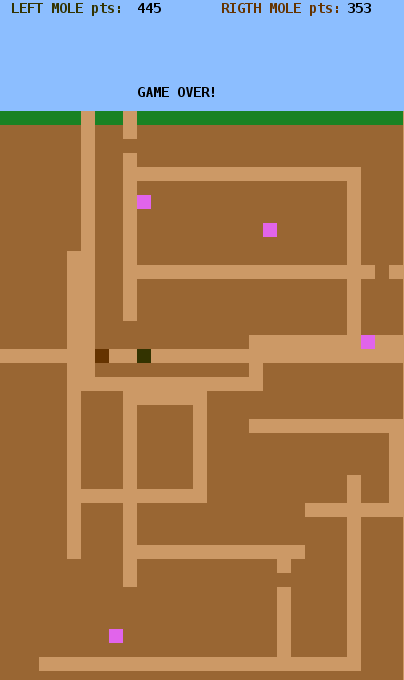
\includegraphics[width=1.0\textwidth]{../img/blockbattle.png}
  \caption{En duell om blockmaskar mellan två lundensiska blockmullvader fångade på bild under intensivt grävanade.}
  \label{lab:blockbattle:fig:game}
\end{figure}
\end{minipage}%
}%
\newlength{\currentparskip}%
\newlength{\currentparindent}%
{
\setlength{\currentparskip}{\parskip}% save the value
\setlength{\currentparindent}{\parindent}% save the value
\hfill%
\begin{minipage}{0.47\textwidth}
\setlength{\parskip}{\currentparskip}% restore the value
\setlength{\parindent}{\currentparindent}% restore the value
\noindent Under denna laboration ska du träna på att deklarera klasser och skapa flera instanser av samma klass. Du tränar även på att bygga ett större program från grunden.

Du ska utveckla ett spel för två spelare som sitter vid samma tangentbord, där den vänstra spelaren styr en blockmullvad med tangenterna A,S,D,W, och den högra spelaren styr en annan blockmullvad med piltangenterna.

I bilden till vänster ser du hur spelet kan se ut. Det finns en ljusbrun och en mörkbrun mullvad. Poängräkningen visas överst i himlen. Det finns fyra rosa blockmaskar (se uppgift \ref{lab:blockmole:task:blockworm} i laboration \code{blockmole}) som mullvadarna tävlar om att försöka fånga. När en blockmask teleporterar sig till en ny slumpmässig position lämnar den jord efter sig. När en mullvad gräver sig upp till gräsytan blir det hål i gräset.
Det ger poäng att gräva tunnlar och att fånga blockmaskar.

Du bestämmer själv hur poängsättningen ska ske och kriteriet för när spelet är slut etc.
\end{minipage}%
}



\subsection{Obligatoriska krav}

Följande funktionella krav ska uppfyllas av ditt program:
\begin{itemize}[nosep, label={$\square$},]
%\item Det ska finnas två blockmullvadar, en för vänster spelare och en för höger spelare, som styrs med ASDW resp. piltangerna.
\item Varje mullvad rör sig i sin aktuella riktning tills användaren ändrar riktning genom att trycka på ''sin'' motsvarande knapp, t.ex. W eller pil-upp.
\item Då en mullvad går i mörkbrun jord ska ljusbruna tunnlar grävas.
\item Då en blockmullvad når fönstrets kant eller himlen ska dess riktning reverseras.
\item Det ska ge poäng att gräva tunnlar.
\item Varje spelares poäng ska visas under spelets gång.
\item Ett spel ska avslutas och \emph{Game over} visas när något valfritt kriterium uppfyllts.
%\item Vid \emph{Game over} ska man kunna välja att avsluta programmet eller spela igen.
\end{itemize}

\noindent Din kod ska utformas enligt dessa design-krav:
\begin{itemize}[nosep, label={$\square$}]
\item Ett \code{Game} skapas i huvudprogrammet med metoden \code{start} som kör igång spelet.
\item Konstanter ska namnges och placeras i lämpligt kompanjonsobjekt.
\item Varje klass med ev. tillhörande kompanjonsobjekt ska finnas i en egen kodfil och tillhöra paketet \code{blockbattle}.
\item Du ska utgå från klasserna som du implementerat i uppgift \ref{exe:classes:labprep} i övning \texttt{\ExeWeekFIVE}.
\item Klassen \code{BlockWindow} omvandlar till interna fönsterkoordinater. Övriga klasser ska använda block-koordinater.
\end{itemize}


\subsection{Valbara krav -- välj minst ett}

Du ska implementera minst ett (gärna flera) av dessa krav:
\begin{itemize}[nosep, label={$\square$}]
\item Det ska finnas lagom många blockmaskar (se labb \code{blockmole} uppg. \ref{lab:blockmole:task:blockworm},  sid. \pageref{lab:blockmole:task:blockworm}).
\item Blockmullvadarna ska även ha ett attribut som representerar hälsan, t.ex. ett numeriskt värde mellan 0 och 100. Hälsan ska försvagas något när man gräver tunnlar. Hälsan ska synas i spelfönstret, t.ex. som en sekvens med röda block i himlen som indikerar andelen av maxhälsan för resp. spelare.
\item Att springa på gräset ska påverka poäng och/eller hälsa.
\item Att fånga blockmask ska påverka poäng och/eller hälsa.
\item Det ska finnas gula blockdiamanter som ger många poäng om man tar dem först.
\item Det ska vid spelstart gå att välja namn på respektive blockmullvad och namnet ska synas i spelet vid poängutskriften.
\item Det ska gå fortare att gå i gångar jämfört med att gräva i jord.
\item Om en blockmullvad fångar en blockmask ska dess grävhastighet öka.
\item Om en blockmullvad krockar med en annan blockmullvad ska något hända, t.ex. att dess riktning reverseras.
\item Visa \emph{highscore} vid \emph{Game Over}.  Highscore sparas med \code{introprog.IO} i en fil som skapas om den inte finns annars läses in vid uppstart om den finns och uppdateras vid behov. Spara hela highscore-listan eller bara högsta poäng hittills.
\end{itemize}

\subsection{Förebredelser inför redovisningen}
\Checkpoint\noindent Innan du redovisar din implementation ska du muntligt kunna redogöra för följande:
\begin{itemize}[nosep, label={$\square$}]
  \item Studera någon annans spel och ge din kamrat minst ett tips om hur kodens läsbarhet kan förbättras. Skriv ner dina tips och beskriv dem vid redovisningen.
  \item Beskriv vilka åtgärder du gjort för att din kod ska vara lätt att läsa och förstå.
  \item Beskriv hur du stegvis utvecklat ditt program från enklare till mer avancerad funktionalitet, samt vilka buggar du upptäckt och fixat.
  \item Beskriv vilket eller vilka valfria krav som din implementation uppfyller.
  \item Beskriv hur du hade behövt ändra i klassen \code{Mole} för att det ska gå att skriva\\\code{new Mole().move().move().reverseDir().move()}
\end{itemize}

\subsection{Tips och förslag}

\begin{enumerate}[leftmargin=*]
  \item \textbf{Många små steg.} Kör kompilering under ändringsbevakning med \code{--watch} i ett eget terminalfönster, så att du vid varje ändring kan rätta ev. kompileringsfel. Kör och testa ditt program ett annat terminalfönster.

  \item \textbf{Inför bra namn}. Din kod blir lättare att läsa och ändra i om du hittar på bra namn på medlemmar och lägger dem på lämpligt ställe. T.ex. kan du samla globala spel-konstanter i kompanjonsobjektet till klassen \code{Game}. Du kan bygga vidare på nedan kod och lägga till medlemmar allteftersom du upptäcker att de behövs. Nedan finns exempelvis en funktion som ger bakgrundsfärgen för en viss y-koordinat, vilken är användbar när du ska återställa bakgrunden efter att en mullvad har flyttat sig.
\scalainputlisting[basicstyle=\ttfamily\fontsize{10}{12}\selectfont]{../workspace/w06_blockbattle/Game.scala}
% \begin{CodeSmall}
% object Game {
%   val windowSize = (30, 50)
%   val windowTitle = "EPIC BLOCK BATTLE"
%   val blockSize = 14
%   val skyRange    = 0 to 7
%   val grassRange  = 8 to 8
%   object Color { ??? }
%   def backgroundColorAtDepth(y: Int): java.awt.Color = ???
% }
%
% class Game(
%   val leftPlayerName: String  = "LEFT",
%   val rightPlayerName: String = "RIGHT"
% ) {
%  import Game.* // direkt tillgång till namn på medlemmar i kompanjon
%
%  val window    = new BlockWindow(windowSize, windowTitle, blockSize)
%  val leftMole  = ???
%  val rightMole = ???
%
%  def drawWorld(): Unit = ???
%
%  def eraseBlocks(x1: Int, y1: Int, x2: Int, y2: Int): Unit = ???
%
%  def update(mole: Mole): Unit = ???  // update, draw new, erase old
%
%  def gameLoop(): Unit = ???
%
%  def start(): Unit = {
%    println("Start digging!")
%    println(s"$leftPlayerName ${leftMole.keyControl}")
%    println(s"$rightPlayerName ${rightMole.keyControl}")
%    drawWorld()
%    gameLoop()
%  }
% }
% \end{CodeSmall}

 \item \textbf{Dela upp din kod i funktioner.} Din kod blir lättare att läsa och ändra i om du delar upp den i många små funktioner med bra namn. I \code{Game}-klassen ovan finns exempel på några användbara funktioner. Allteftersom du utvidgar ditt program kan du lägga till fler funktioner som t.ex. heter \code{showPoints}, \code{gameOver}, etc.

\item \textbf{Tänk igenom den övergripande strukturen.} Programmet du ska skriva i denna laboration är större än det du gjort tidigare. Det är därför viktigt att tänka igenom strukturen på ditt program, vilka klasser som har hand om vad och hur de samarbetar. Diskutera gärna med handledare om du är osäker på hur de koddelar du utvecklat i föregående veckas övning \ref{exe:classes:labprep}, klasserna \code{Pos}, \code{KeyControl}, \code{Mole} och \code{BlockWindow}, är tänkt at samverka. Var noga med att testa så de olika klasserna och deras metoder fungerar var för sig.     

\item \textbf{Utformning av \texttt{gameLoop()}}. I ett spel behövs en s.k. spel-loop \Eng{game loop} som upprepar den kod som ska köras vid varje ny skärmbild, ofta kallad \emph{frame}. I varje runda i spel-loopen sker uppdatering av data och ritning i spelfönstret, samt en lämplig fördröjning. En skiss på en typisk spel-loop visas nedan:
\begin{CodeSmall}
  var quit = false
  val delayMillis = 80

  def gameLoop(): Unit = 
    while !quit do
      val t0 = System.currentTimeMillis
      handleEvents()    // ändrar riktning vid tangenttryck etc.
      update(leftMole)  // flyttar, ritar, suddar, etc.
      update(rightMole)

      val elapsedMillis = (System.currentTimeMillis - t0).toInt
      Thread.sleep((delayMillis - elapsedMillis) max 0)
    end while
  end gameLoop
\end{CodeSmall}

\item \textbf{Hantering av händelser.} Ett \code{BlockWindow}, som du implementerade i uppgift \ref{exe:classes:labprep} i övning \texttt{\ExeWeekFIVE}, kan via anrop av \code{nextEvent} ge   \code{KeyPressed(key)} vid knapptryck och \code{WindowClosed} vid fönsterstängning. Om ingen händelse finns att behandla returneras \code{Undefined}. Använd en loop som betar av alla händelser tills \code{Undefined} påträffas, enligt nedan:

\begin{CodeSmall}
  def handleEvents(): Unit = 
    var e = window.nextEvent()
    while e != BlockWindow.Event.Undefined do
      e match 
        case BlockWindow.Event.KeyPressed(key) =>
          ???  // ändra riktning på resp. mullvad

        case BlockWindow.Event.WindowClosed =>
          ???  // avsluta spel-loopen
      
      e = window.nextEvent()
    end while
  end handleEvent
\end{CodeSmall}

\item \textbf{Flimmerfri grafik.} För att minska mängden flimmer \Eng{flicker} är det bäst att i varje iteration i spel-loopen (1) bara rita om det som ändrats för att minimera tiden som spenderas på att rita, och (2) vid ändringar rita nya delar före att gamla delar raderas. För att slippa mullvadsflimmer kan du ''\emph{rita först -- sudda sen}'' enligt nedan.\footnote{Inom spelutveckling använder man oftast istället så kallad \emph{double buffering} (eller till och med \emph{triple buffering}) för att få helt flimmerfri grafik. Det ligger dock bortom kursen och stöds inte av \code{PixelWindow}.}

% \begin{CodeSmall}
% val oldMolePos = mole.pos                  // save
% mole.move()                                // update
% window.setBlock(mole.pos, mole.color)      // draw new
% window.setBlock(oldMolePos, Color.tunnel)  // erase old
% \end{CodeSmall}

\begin{CodeSmall}
window.setBlock(mole.nextPos, mole.color) // draw new
window.setBlock(mole.pos, Color.tunnel)   // erase old
mole.move()                               // update
\end{CodeSmall}

\end{enumerate}


%!TEX encoding = UTF-8 Unicode

%!TEX root = ../compendium1.tex

\chapter{Arv, Gränssnitt}
\begin{itemize}[nosep]
\item klasser
\item arv
\item polymorfism
\item likhet
\item equals
\item accessregler
\item private
\item public
\item protected
\item private[this]
\item trait
\item inmixning
\item Any
\item AnyVal
\item AnyRef
\item Nothing\end{itemize}
\clearpage\section{Teori}
%!TEX encoding = UTF-8 Unicode
%!TEX root = ../lect-w07.tex

\Subsection{Vad är en sekvens?}

\ifkompendium\else
{
  \setbeamercolor{background canvas}{bg=black}
  \frame[plain]{\centering\Huge\textbf{\color{pink}{ORDNINGEN}\\SPELAR\\ROLL}}
}
\fi


\begin{Slide}{Vad är en sekvens?}  
\begin{itemize}
\item En sekvens är en \Emph{följd av element} som
  \begin{itemize}
  \item har \Alert{ordningsnummer} (t.ex. numrerade från noll)
  \item är av en viss \Alert{typ} (t.ex. heltal).
  \end{itemize}
  \pause
\item En sekvens kan innehålla flera element som är lika.
\item En sekvens kan vara \Alert{tom} och har då längden noll.
\item Exempel på en icke-tom sekvens med dubbletter:
\begin{REPLnonum}
scala> val xs = Vector(42, 0, 42, -9, 0, 5)
xs: scala.collection.immutable.Vector[Int] =
  Vector(42, 0, 42, -9, 0, 5)
\end{REPLnonum}
\pause
\item \Emph{Indexering} ger ett element via dess ordningsnummer:
\begin{REPLnonum}
scala> xs(2)
res0: Int = 42

scala> xs.apply(2)
res1: Int = 42
\end{REPLnonum}
\end{itemize}
\end{Slide}

\begin{Slide}{Exempel: En sträng är en sekvens av tecken}
\begin{REPLnonum}
scala> "haj po daj"
\end{REPLnonum}
Längd? 
Vad ligger på första platsen?
Elementtyp?
Dubbletter?
\pause
\begin{REPLnonum}
scala> "haj po daj".length
res1: Int = 10

scala> "haj po daj".apply(0)
res2: Char = h

scala> "haj po daj"(0)
res3: Char = h

scala> "haj po daj".distinct
res4: String = haj pod
\end{REPLnonum}

\end{Slide}


\begin{Slide}{Iterera över element i en sekvens}
\begin{itemize}
\item Att \Emph{iterera} \Eng{iterate}, ä.k. traversera \Eng{traverse}, innebär att \Alert{gå igenom} och behandla element i en samling. 
\item Exempel på iterering med \code{foreach}, \code{map}, \code{for}:
\begin{REPLnonum}
scala> val xs = Vector(1,2,3)
val xs: Vector[Int] = Vector(1, 2, 3)

scala> xs.foreach(x => println(x + 1)) 
2
3
4

scala> xs.map(_ + 1)
val res0: Vector[Int] = Vector(2, 3, 4)

scala> for x <- xs yield x - 1
val res1: Vector[Int] = Vector(0, 1, 2)

\end{REPLnonum}
\end{itemize}
\end{Slide}

\begin{Slide}{Lägg till i början och i slutet av en sekvens}
  \begin{itemize}
  \item Med metoderna \code{+:} och \code{:+} kan du skapa en ny sekvens med nya element tillagda i början resp. i slutet.
  \item Minnesregel: ''\Alert{Colon on the collection side}''
  \begin{REPLnonum}
  scala> val xs = Vector(1,2,3)
  scala> 42 +: xs         // ger ny Vector(42, 1, 2, 3)
  scala> xs :+ 42         // ger ny Vector(1, 2, 3, 42)
  \end{REPLnonum}
  \pause
  \item Semantik: operatornotation med operatorer som \Emph{slutar med kolon} är \Alert{högerassociativa}
  \item Anropet \code{42 +: xs} skrivs av kompilatorn om till \code{xs.+:(42)}
  \begin{REPL}
  scala> xs.+:(42)
  res4: scala.collection.immutable.Vector[Int] = Vector(42, 1, 2, 3)
  \end{REPL}
  \pause
  \item Konkatenering (sammanfogning) av sekvenser: \code{xs ++ ys}
  
  \end{itemize}
\end{Slide}


\begin{Slide}{Egenskaper hos några sekvenssamlingar i Scala}
\vspace{-0.5em}
\begin{itemize}\SlideFontSmall

\item \code{Vector}
  \begin{itemize}\SlideFontSmall
  \item \Emph{Oföränderlig}. Snabb på att skapa kopior med små förändringar.
  \item Allsidig prestanda: \Emph{bra till det mesta}.
  \end{itemize}

\item \code{List}
  \begin{itemize}\SlideFontSmall
  \item \Emph{Oföränderlig}. Snabb på att skapa kopior med små förändringar.
  \item Snabb indexering \& uppdatering \Emph{i början}.
  \item Smidig \& snabb vid \Emph{rekursiva} algoritmer.
  \item Långsam vid upprepad \Alert{indexering} på godtyckliga ställen.
  \end{itemize}

\item \code{ArrayBuffer}
  \begin{itemize}\SlideFontSmall
  \item \Alert{Föränderlig}: \Emph{snabb indexering \& uppdatering}.
  \item Kan \Emph{ändra storlek} efter allokering. Snabb att indexera överallt.
  \end{itemize}

\item \code{ListBuffer}
  \begin{itemize}\SlideFontSmall
  \item \Alert{Föränderlig}: snabb indexering \& uppdatering \Emph{i början}.
  \item Snabb om du bygger upp sekvens genom många tillägg i början.
  \end{itemize}

\item \code{Array} (använd fr.o.m. Scala 2.13 hellre \code{ArraySeq})
  \begin{itemize}\SlideFontSmall
  \item \Alert{Föränderlig}: \Emph{snabb indexering \& uppdatering}.
  \item Kan \Alert{ej ändra storlek}; storlek ges vid allokering.
  \item Har särställning i JVM: ger snabb allokering och access.
  \end{itemize}

\end{itemize}
\end{Slide}

\begin{Slide}{I stället för Array: \texttt{ArraySeq} (Scala >2.13)}
Nytt i Scala 2.13:
\begin{itemize}
  \item \code{collection.mutable.ArraySeq} fungerar lika bra som, eller bättre än \code{Array}
  \item \url{https://stackoverflow.com/questions/5028551/array-vs-arrayseq-comparison}
  \item \code{collection.immutable.ArraySeq} fungerar som en Array som inte kan ändras
  \item \code{WrappedArray} är från 2.13 \textit{deprecated} (på väg bort)
\end{itemize}
{\SlideFontTiny Fördjupning: Sammanfattning av prestanda för olika samlingar: \href{https://docs.scala-lang.org/overviews/collections-2.13/performance-characteristics.html}{docs.scala-lang.org/overviews/collections-2.13/performance-characteristics.html}
}
\end{Slide}

\begin{Slide}{Vilken sekvenssamling ska jag välja?}\SlideFontSmall
\vspace{-0.5em}
\begin{itemize}
\item Välj \code{Vector} om ...
  \begin{itemize}\SlideFontTiny
  \item[a)] du vill ha oföränderlighet: \code{val xs = Vector[Int](1,2,3)}
  \item[b)] du behöver föränderlighet (notera \code{var}):\\ \code{var xs = Vector.empty[Int]}
  \item[c)] du ännu inte vet vilken sekvenssamling som är bäst; du kan alltid ändra efter att du mätt prestanda och kollat flaskhalsar vid upprepade körningar.
  \end{itemize}

\item Välj \code{List} om ...
  \begin{itemize}\SlideFontTiny
  \item[] du har en \Alert{rekursiv} sekvensalgoritm och/eller \Alert{mestadels jobbar i början}.
  \end{itemize}

\item Välj \code{ArrayBuffer} om ...
  \begin{itemize}\SlideFontTiny
  \item[] det behövs av prestandaskäl och du \Alert{inte} vet storlek vid allokering:\\
  \code{val xs = scala.collection.mutable.ArrayBuffer.empty[Int]}
  \end{itemize}

\item Välj \code{ListBuffer} om ...
  \begin{itemize}\SlideFontTiny
  \item[] det behövs av prestandaskäl och du bara behöver lägga till i början:\\ \code{val xs = scala.collection.mutable.ListBuffer.empty[Int]}
  \end{itemize}

\item Välj \code{Array} eller \code{ArraySeq} om ...
  \begin{itemize}\SlideFontTiny
  \item[] det verkligen behövs av prestandaskäl och du \Alert{vet} storlek vid allokering:\\
  \code{val xs = Array.fill(initSize)(initValue)}
  \end{itemize}

\end{itemize}
\end{Slide}

\begin{Slide}{Några konstigheter med Array}
\begin{itemize}
\item Referenslikhet istf innehållslikhet: 
\begin{REPLnonum}
scala> Vector(1,2,3) == Vector(1,2,3)
val res0: Boolean = true

scala> Array(1,2,3) == Array(1,2,3)
val res1: Boolean = false  // aaargh!!
\end{REPLnonum}
\item Special-syntax för att skapa utan explicit initialisering: \\
{\SlideFontSmall\code{val xs = new Array[String](1000)  // 1000 null-referenser}}
\item Fungerar inte lika bra med generiska typer:
\begin{REPLnonum}
scala> def box[T](x: T) = Vector[T](x)  //funkar fint

scala> def abox[T](x: T) = Array[T](x)
  error: No ClassTag available for T
\end{REPLnonum}
\end{itemize}
\end{Slide}

\begin{Slide}{Oföränderlig eller förändringsbar?}
\begin{itemize}
\item \Emph{Oföränderlig}:  Kan ej ändra elementreferenserna, men effektiv på att skapa kopia som är (delvis) förändrad \Emph{Vector} eller \Emph{List}

\item \Alert{Förändringsbar}: kan ändra elementreferenserna
  \begin{itemize}
  \item Kan \Alert{ej ändra storlek} efter allokering: \\ \Emph{Array} eller \Emph{ArraySeq}: indexera och uppdatera varsomhelst
  \item Kan även ändra storlek efter allokering:
  \\\Alert{ArrayBuffer} eller \Alert{ListBuffer}
  %\\ Java: \Alert{ArrayList} eller \Alert{LinkedList}
  \end{itemize}
\item \Emph{Ofta funkar oföränderlig sekvenssamling utmärkt}, men om man \Alert{efter prestandamätning} upptäcker en flaskhals kan man ändra från \Emph{Vector} till t.ex. \Emph{ArrayBuffer}.
\end{itemize}
\end{Slide}



\Subsection{Vad är en sekvensalgoritm?}



\begin{Slide}{Vad är en sekvensalgoritm?}\SlideFontTiny
\begin{itemize}
\item En algoritm är en stegvis beskrivning av lösningen på ett problem.
\item En \textbf{sekvensalgoritm} är en algoritm där \Emph{element i sekvens} utgör en viktig del av \Alert{problembeskrivningen} och/eller \Alert{lösningen}.
\item Exempelproblem: sortera en sekvens av personer efter deras ålder.
\pause
\item \Alert{Sju} ofta återkommande programmeringsproblem som löses med en sekvensalgoritm:
\begin{itemize}\SlideFontTiny
\item \Emph{Kopiering} av alla element i en sekvens till en \Alert{ny} sekvens
\item \Emph{Uppdatering} av sekvensen: ta bort, lägga till, ändra \Emph{enskilda} element
\item \Emph{Transformering}: applicera en \Alert{funktion} på \Emph{alla} element   
\item \Emph{Filtrering}: urval av vissa element som uppfyller ett \Alert{villkor}
\item \Emph{Sökning} efter ett element som uppfyller ett \Alert{sökkriterium}
\item \Emph{Sortering} enligt någon \Alert{ordning}
\item \Emph{Registrering} av \Alert{frekvens} av element med vissa \Alert{egenskaper}
\end{itemize}
\end{itemize}
\href{https://youtu.be/0ArlUSVDQIw?t=27s}{\textbf{KUT FSSR}} 
\end{Slide}

\ifkompendium\else
{
  \setbeamercolor{background canvas}{bg=black}
  \frame[plain]{\centering\Huge\textbf{\color{pink}{ORDNINGEN\\SPELAR\\ROLL}\\\color{red}{KUT FSSR}}}
}
\fi



\Subsection{Använda färdiga sekvenssamlingsmetoder}


\begin{Slide}{Använda färdiga sekvenssamlingsmetoder}
\begin{itemize}\SlideFontSmall
\item Standardbiblioteket i Scala innehåller flera olika samlingar som har sekvensegenskaper, t.ex. \code{Vector} och \code{ArrayBuffer}, som erbjuder olika möjligheter och har olika prestanda beroende på vad man vill göra.
\item Scala 3 använder samma samlingsbibliotek som i Scala 2.13, se intro:  \url{https://docs.scala-lang.org/overviews/collections-2.13/introduction.html} 

\item Ofta kan man implementera sekvensalgoritmer genom anrop av en eller flera \Alert{färdiga} metoder.

\item Dessa färdiga metoder är \Emph{optimerade och vältestade} och är att föredra om möjligt.

\item Studera Scalas api-dokumentation och kursens quickref för att se vad man kan göra med färdiga metoder.

\item Det är \Emph{lärorikt} att ''\Alert{uppfinna hjulet}'' och implementera några sekvensalgoritmer \Emph{själv} för bättre förståelse, även om de redan finns färdiga i Scalas samlingsbibliotek.

\end{itemize}
\end{Slide}



\begin{Slide}{Några användbara samlingsmetoder vid implementation av sekvensalgoritmer}
\SlideFontTiny
\begin{tabular}{@{}l l}
\code|xs.map(f)|           & transformering, motsv. \code|for x <- xs yield f(x)| \\
\code|xs.map(x => x)|    & kopiering, motsv. \code|for x <- xs yield x| \\
\code|xs.filter(p)|        & filtrering, ta med x om p(x)\\
\code|xs.filterNot(p)|     & filtrering, ta med x om !p(x)\\
\code|xs.distinct|        & filtrering, ta bort dubbletter \\
\code|xs.take(n)|          & ny sekvens med de första n elements, resten skippade\\ 
\code|xs.drop(n)|          & ny sekvens där de första n elements är skippade\\ 
\code|xs.takeWhile(p)|     & filtrera, ta med i början så länge p(x)  \\
\code|xs.dropWhile(p)|     & filtrera, skippa i början så länge p(x)  \\
\code|xs.find(p)|       & sök framifrån efter första element x där p(x) är sant\\
\code|xs.indexOf(x)|       & sök framifrån efter index för element som är samma som x \\
\code|xs.lastIndexOf(x)|   & sök bakifrån efter index för element som är samma som x \\
\code|xs.sorted|          & sortera med inbyggd (implicit given) ordning \\
\code|xs.sorted.reverse| & sortera i omvänd ordning \\
\code|xs.sortBy(f)|        & sortera i ordning enligt f(x)\\
\code|xs.sortWith(lt)|     & sortera enligt ''less than''-funktionen \code|lt: (A, A) => Boolean|\\
\code|xs.count(p)|         & räkna antalet element där p(x) är sant
\end{tabular}

\vspace{0.5em}%
\Emph{Lär dig fler smidiga metoder i} \Alert{quickref}
\end{Slide}

\begin{Slide}{Uppdaterad sekvens med kraftfulla metoden \texttt{patch}}
  Metoden \code{patch} kan användas så: \code{xs.patch(fromPos, ys, nbrReplaced)} \\för att skapa en \Alert{ny} sekvens där \Emph{ett} eller \Emph{flera} element i xs är...  
  \begin{itemize}
    \item utbytta \Eng{replaced}
    \item borttagna \Eng{removed}
    \item tillagda \Eng{inserted}
  \end{itemize}
  .. med nya element ur \code{ys} 
\begin{REPL}
scala> val xs = Vector(1,2,3)

scala> xs.patch(2, Vector(-1), 1)     // replaced one elem
res0: scala.collection.immutable.Vector[Int] = Vector(1, 2, -1)

scala> xs.patch(1, Vector(42), 0)     // inserted one elem
res11: scala.collection.immutable.Vector[Int] = Vector(1, 42, 2, 3)

scala> xs.patch(0, Vector(), 2)       // removed two elems
res2: scala.collection.immutable.Vector[Int] = Vector(3)
 
\end{REPL}
\end{Slide}

\begin{Slide}{Använda for-uttryck för filtrering med hjälp av gard}
I ett for-uttryck kan man ha en \Emph{gard} \Eng{guard} i form av ett booleskt uttryck efter nyckelordet \code{if}. Då kommer uttrycket efter \code{yield} bara göras om gard-uttrycket är sant.

\vspace{1em}

Syntaxen är så här: (parenteser behövs ej runt gard-uttrycket)
\begin{Code}[basicstyle=\ttfamily\SlideFontSize{12}{14}]
for x <- xs if uttryck1 yield uttryck2
\end{Code}
\pause
Exempel:
\begin{REPLnonum}
scala> val udda = for x <- 1 to 6 if x % 2 == 1 yield x
\end{REPLnonum}
\pause
\code{udda} blir \code{Vector(1, 3, 5)}
\end{Slide}


\begin{Slide}{Använda samlingsmetoden \texttt{filter} för filtrering}
Alla samlingar i \code{scala.collection} har metoden \code{filter}. Den har ett predikat som parameter \code{p: T => Boolean} och ger en ny samling med de element för vilka predikatet är sant.
\begin{Code}[basicstyle=\ttfamily\SlideFontSize{12}{14}]
xs.filter(p)
\end{Code}
\pause
Exempel: Antag att \code{xs} är \code{(1 to 6).toVector}
\begin{REPLnonum}
xs.filter(_ % 2 == 1)
\end{REPLnonum}
\pause
uttryckets resultat blir \code{Vector(1, 3, 5)}, vilket motsvarar:
\begin{Code}[basicstyle=\ttfamily\SlideFontSize{10}{13}]
for x <- xs if x % 2 == 1 yield x
\end{Code}
\pause
I själva verket skriver Scala-kompilatorn om for-uttryck med gard till anrop av metoden \code{filter} före kodgenerering sker.
\end{Slide}


\begin{Slide}{Vanliga sekvensproblem som funktionshuvuden}
Indata och utdata för några vanliga sekvensproblem:
\begin{Code}
def copy(xs: Vector[Int]): Vector[Int] = ???

def filter(xs: Vector[Int], p: Int => Boolean): Vector[Int] = ???

def findIndices(xs: Vector[Int], p: Int => Boolean): Vector[Int] = ???

def sort(xs: Vector[Int]): Vector[Int] = ???

def freq(xs: Vector[Int]): Vector[(Int, Int)] = ???  // (heltal, frekvens)
\end{Code}
Övning: Hur implementera dessa med \code{for}-uttryck och/eller färdiga samlingsmetoder?\\
\Emph{Tips:} För \code{sort}\&\code{freq} se \code{sorted}, \code{distinct}, \code{count} i \href{http://cs.lth.se/pgk/quickref/}{quickref}
\end{Slide}


\begin{Slide}{Implementation av sekvensproblem med \texttt{for}-uttryck och/eller färdiga samlingsmetoder}
\begin{Code}
def copy(xs: Vector[Int]): Vector[Int] = for x <- xs yield x

def filter(xs: Vector[Int], p: Int => Boolean): Vector[Int] =
  for x <- xs if p(x) yield x

def findIndices(xs: Vector[Int], p: Int => Boolean): Vector[Int] =
  (for i <- xs.indices if p(xs(i)) yield i).toVector

def sort(xs: Vector[Int]): Vector[Int] = xs.sorted // mer om sortering sen

def freq(xs: Vector[Int]): Vector[(Int, Int)] = // mer om registrering snart
  for x <- xs.distinct yield x -> xs.count(_ == x)
\end{Code}
Övning: Hur implementera dessa med \code{map} och \code{filter} och/eller andra färdiga samlingsmetoder?
\end{Slide}

\begin{Slide}{Implementation av sekvensproblem med \texttt{map}, \texttt{filter}}
\begin{Code}
def copy(xs: Vector[Int]): Vector[Int] = xs.map(x => x)

def filter(xs: Vector[Int], p: Int => Boolean): Vector[Int] = xs.filter(p)

def findIndices(xs: Vector[Int], p: Int => Boolean): Vector[Int] =
  xs.indices.filter(i => p(xs(i))).toVector

def sort(xs: Vector[Int]): Vector[Int] = xs.sorted // mer om sortering sen

def freq(xs: Vector[Int]): Vector[(Int, Int)] = // mer om registrering snart
  xs.distinct.map(x => x -> xs.count(_ == x))
\end{Code}
%Fördjupningsövning: Hur göra dessa metoder generiska för alla sekvenssamlingar av typen \code{Seq[T]}?
\end{Slide}


\begin{Slide}{Hierarki av samlingstyper i \texttt{scala.collection} v2.13}

  \begin{multicols}{2}
  \begin{tikzpicture}[sibling distance=5.0em,->,>=stealth', inner sep=3pt, %scale=0.5,
    every node/.style = {shape=rectangle, draw, align=center,font=\small\ttfamily},
    class/.style = {fill=blue!20},
    trait/.style = {rounded corners, fill=red!20}]
    \node[trait] {Iterable}
        child { node[trait] {Seq} }
        child { node[trait] {Set} }
        child { node[trait] {Map} }
      ;
  \end{tikzpicture}
  
  \columnbreak
  
  {\SlideFontTiny
  
  \code{Iterable} har metoder som är implementerade med hjälp av: \\
  \code{def foreach[U](f: Elem => U): Unit}\\
  \code{def iterator: Iterator[A] }
  
}

\begin{itemize}\SlideFontTiny
  \item[] \code{Seq}: ordnade i sekvens
  \item[] \code{Set}: unika element
  \item[] \code{Map}: par av (nyckel, värde)
  \end{itemize}
  
  
  \end{multicols}
  
  {\SlideFontSmall Samlingen \Emph{\texttt{Vector}} är en \code{Seq} som är en \code{Iterable}. \\ \vspace{0.5em}\pause
  De konkreta samlingarna är uppdelade i dessa paket:\\
  \code{scala.collection.immutable} \hfill där flera är \Emph{automatiskt} importerade\\
  \code{scala.collection.mutable}  \hfill som \Alert{måste importeras} explicit\\\pause
  (undantag: primitiva \code{scala.Array})
  }
\end{Slide}
  


\begin{Slide}{Lämna det öppet: använd \texttt{Seq}}\SlideFontSmall
Typen \Emph{\code{collection.immutable.Seq}} är supertyp till alla sekvenssamlingar i \code{collection.immutable}.
\pause Exempel: kopiering av sekvens:
\begin{itemize}
\item Kopiering av \Alert{specifik} heltalssekvens:
\begin{Code}
def copyIntVector(xs: Vector[Int]): Vector[Int] = for x <- xs yield x
\end{Code}

\item Kopiering som fungerar för alla oföränderliga heltalssekvenser:
\begin{Code}
def copyIntSeq(xs: Seq[Int]): Seq[Int] = for x <- xs yield x
\end{Code}
\end{itemize}
\pause
\begin{REPL}
scala> val xs = Vector(1,2,3)
xs: Vector[Int] = Vector(1, 2, 3)

scala> val ys = copyIntVector(xs)
ys: Vector[Int] = Vector(1, 2, 3)

scala> val zs = copyIntSeq(xs)
val zs: Seq[Int] = Vector(1, 2, 3)
\end{REPL}
%  Någon lämplig specifik samling som är subtyp till \code{Seq[T]} väljs automatiskt. \\
% (Mer om typparametrar och supertyper/subtyper senare i kursen.)
% \begin{Code}[basicstyle=\ttfamily]
% def varannanBaklänges[T](xs: Seq[T]): Seq[T] =
%   for i <- xs.indices.reverse by -2 yield xs(i)
% \end{Code}
% Fungerar med alla sekvenssamlingar:
% \begin{REPLnonum}
% scala> varannanBaklänges(Vector(1,2,3,4,5))
% res0: Seq[Int] = Vector(5, 3, 1)
%
% scala> varannanBaklänges(List(1,2,3,4,5))
% res1: Seq[Int] = List(5, 3, 1)
%
% scala> varannanBaklänges(collection.mutable.ListBuffer(1,2))
% res2: Seq[Int] = Vector(2)
% \end{REPLnonum}
% Scalas standardbibliotek returnerar ofta lämpligaste specifika sekvenssamlingen som är subtyp till \texttt{Seq[T]}.
\end{Slide}
  
\begin{Slide}{Implementation med generiska funktioner}\SlideFontSmall
Genom att generalisera funktionshuvudena blir våra lösningar användbara för \Alert{alla} sekvenser av typen \code{Seq[T]}, där den obundna \Emph{typparametern} \code{T} vid anrop kan bindas till godtycklig typ. (Mer om typparametrar senare.)
\begin{Code}
def copy[T](xs: Seq[T]): Seq[T] = xs.map(x => x)

def filter[T](xs: Seq[T], p: T => Boolean): Seq[T] = xs.filter(p)

def findIndices[T](xs: Seq[T], p: T => Boolean): Seq[Int] =
  xs.indices.filter(i => p(xs(i))).toVector

def sort[T: Ordering](xs: Seq[T]): Seq[T] = xs.sorted // mer om Ordering sen

def freq[T](xs: Seq[T]): Seq[(T, Int)] =
  xs.distinct.map((_, xs.count(_ == x)))
\end{Code}
\pause
Standardbibliotekets metoder försöker ordna så att det blir samma konkreta typ in som ut, men ibland väljs annan lämplig konkret samling, t.ex. kan en \code{Array} bli en \code{ArrayBuffer}. 
\end{Slide}

\begin{Slide}{Använda Java-samlingar i Scala med \texttt{CollectionConverters}}\SlideFontSmall
Med hjälp av \code{import scala.jdk.CollectionConverters.*} \\
får man smidig \Emph{interoperabilitet} med Java och dess standardbibliotek, \\
speciellt metoderna \Alert{\code{asJava}} och \Alert{\code{asScala}}:
\begin{REPL}
scala> import scala.jdk.CollectionConverters.*

scala> Vector(1,2,3).asJava
res0: java.util.List[Int] = [1, 2, 3]

scala> val xs = new java.util.ArrayList[String]()
xs: java.util.ArrayList[String] = []

scala> xs.add("hej")
res1: Boolean = true

scala> xs.asScala
res2: scala.collection.mutable.Buffer[String] = Buffer(hej)
\end{REPL}

\noindent Läs mer här: %
\ifkompendium\\\fi%
\scriptsize%
\url{https://docs.scala-lang.org/overviews/collections-2.13/conversions-between-java-and-scala-collections.html}

\end{Slide}


\begin{Slide}{Fördjupning: Skapa generisk Array}\SlideFontTiny
\begin{itemize}
\item I JVM bytekod går det tyvärr \Alert{inte} att skapa en primitiv generisk array.

\item Maskinkoden måste istället skapa en array av den mest generella referenstypen \code{Object} 
och sedan \Alert{typtesta och typkonvertera under körtid}.\\ Se t.ex. Java-implementationen av \code{ArrayList}:\\\href{http://developer.classpath.org/doc/java/util/ArrayList-source.html}{http://developer.classpath.org/doc/java/util/ArrayList-source.html} %på rad 119
\item[]
\item Men det \Emph{\emph{går}} att skapa en generisk array i Scala (men inte i Java). Då behövs en \code{reflect.ClassTag} som möjliggör typinformation vid körtid för arrayer. \\
\begin{REPLsmall}
scala> def fyll[T](n: Int, x: T): Array[T] = Array.fill(n)(x)
-- Error:
1 |def fyll[T](n: Int, x: T): Array[T] = Array.fill(n)(x)
  |                                                      ^
  |  No ClassTag available for T

scala> def fyll[T: reflect.ClassTag](n: Int, x: T): Array[T] = Array.fill(n)(x)

scala> fyll(42, "hej")
res2: Array[String] = Array(hej, hej, hej, hej, hej, hej, hej, hej, hej, hej, hej, hej, hej, hej, hej, hej, hej, hej, hej, hej, hej, hej, hej, hej, hej, hej, hej, hej, hej, hej, hej, hej, hej, hej, hej, hej, hej, hej, hej, hej, hej, hej)

\end{REPLsmall}
\item Kompilatorn skapar då maskinkod som automatiskt gör typkonverteringarna.

\end{itemize}
\end{Slide}

%!TEX encoding = UTF-8 Unicode
%!TEX root = ../lect-w07.tex

%%%

\Subsection{Repeterade parametrar}

\begin{Slide}{Repeterade parametrar blir sekvens}\SlideFontSmall
Med en asterisk efter parametertypen kan antalet argument variera:
\begin{Code}[basicstyle=\fontsize{10}{12}\selectfont\ttfamily]
def sumSizes(xs: String*): Int = xs.map(_.length).sum
\end{Code}
\begin{REPLnonum}
scala> sumSizes("Zaphod")
res0: Int = 6

scala> sumSizes("Zaphod","Beeblebrox")
res1: Int = 16

scala> sumSizes("Zaphod","Beeblebrox","Ford","Prefect")
res3: Int = 27

scala> sumSizes()
res4: Int = 0
\end{REPLnonum}
Repeterade parametrar \Eng{repeated parameters} blir en sekvens av typen \code{Seq} och som mer specifikt är en \code{ArraySeq}
\end{Slide}


\begin{Slide}{Sekvenssamling som argument till repeterade parametrar}
\begin{Code}[basicstyle=\fontsize{10}{12}\selectfont\ttfamily]
def sumSizes(xs: String*): Int = xs.map(_.size).sum

val veg = Vector("gurka","tomat")
\end{Code}
Om du \emph{redan har} en sekvenssamling så kan du applicera den på en funktion
som har repeterade parametrar med hjälp av en asterisk \code{*} \\
\vspace{1em}Den ska skrivas direkt \Alert{efter} den sekvenssamling, som du vill att kompilatorn ska tolka som en sekvens av argument, så här:
\begin{REPLnonum}
scala> sumSizes(veg*)
res5: Int = 10
\end{REPLnonum}

\end{Slide}

%!TEX encoding = UTF-8 Unicode
%!TEX root = ../lect-w07.tex

%%%

\Subsection{Registrering}

\begin{Slide}{Registrering}
\begin{itemize}
\item \Emph{Registrering} innefattar algoritmer för att räkna antalet förekomster av olika saker.

\item Exempel:
\\\vspace{0.5em}Utfallsfrekvens vid kast med en tärning 1000 gånger:

\vspace{1em}\begin{tabular}{r c l}
utfall & & antal \\ \hline
1 & $\rightarrow$ & 178 \\
2 & $\rightarrow$ & 187 \\
3 & $\rightarrow$ & 167 \\
4 & $\rightarrow$ & 148 \\
5 & $\rightarrow$ & 155 \\
6 & $\rightarrow$ & 165 \\
\end{tabular}
\end{itemize}
\end{Slide}

\begin{Slide}{Registrering av tärningskast i \code{Array}}
Vi låter plats 0 representera antalet ettor, plats 1 representerar antalet tvåor etc. \Alert{Övning}: implementera \code{???}
\begin{REPLnonum}
scala> def rollDice(): Int = ???  //dra slumptal 1-6

scala> val reg = ???  //skapa heltalsarray m 6 platser
reg: Array[Int] = Array(0, 0, 0, 0, 0, 0)

scala> for (i <- 1 to 1000) ???  //kasta tärning, registrera

scala> for (i <- 1 to 6) println(i +": " + reg(i - 1))
1: 178
2: 187
3: 167
4: 148
5: 155
6: 165
\end{REPLnonum}
\end{Slide}


\begin{Slide}{Registrering av tärningskast i \code{Array}}
Vi låter plats 0 representera antalet ettor, plats 1 representerar antalet tvåor etc. \Emph{Lösning}:
\begin{REPLnonum}
scala> def rollDice() = scala.util.Random.nextInt(6) + 1

scala> val reg = new Array[Int](6)
reg: Array[Int] = Array(0, 0, 0, 0, 0, 0)

scala> for (i <- 1 to 1000) reg(rollDice - 1) += 1

scala> for (i <- 1 to 6) println(i +": " + reg(i - 1))
1: 178
2: 187
3: 167
4: 148
5: 155
6: 165
\end{REPLnonum}
\end{Slide}

% \begin{Slide}{Registrering av tärningskast i \code{Map}, imperativ lösning}
% Vi registrerar antalet i en Map[Int, Int] där nyckeln är antalet tärningsögon och värdet är frekvensen.
% \begin{REPLnonum}
% scala> val rnd = new java.util.Random(42L)
% rnd: java.util.Random = java.util.Random@6d946eee
%
% scala> var reg = (1 to 6).map(i => i -> 0).toMap
% reg: scala.collection.immutable.Map[Int,Int] =
%   Map(5 -> 0, 1 -> 0, 6 -> 0, 2 -> 0, 3 -> 0, 4 -> 0)
%
% scala> for (i <- 1 to 1000) {
%          val t = rnd.nextInt(6) + 1
%          reg = reg + ((t, reg(t) + 1))
%        }
%
% scala> reg
% res0:scala.collection.immutable.Map[Int,Int]= Map(5 -> 155,
% 1 -> 178, 6 -> 165, 2 -> 187, 3 -> 167, 4 -> 148)
% \end{REPLnonum}
% \end{Slide}
%
% \begin{Slide}{Registrering av tärningskast i \code{collection.mutable.Map}, imperativ lösning}
% Om vi är bekymrade över prestanda:
% \begin{REPL}
% scala> val rnd = new java.util.Random(42L)
% rnd: java.util.Random = java.util.Random@6d946eee
%
% scala> val initPairs = (1 to 6).map(i => i -> 0)
% initPairs: scala.collection.immutable.IndexedSeq[(Int, Int)] =
% Vector((1,0), (2,0), (3,0), (4,0), (5,0), (6,0))
%
% scala> var reg = scala.collection.mutable.Map(initPairs: _*)
%
% scala> for (i <- 1 to 1000) {
%          val t = rnd.nextInt(6) + 1
%          reg(t) = reg(t) + 1
%        }
%
% scala> reg
% res0: scala.collection.mutable.Map[Int,Int] =
% Map(2 -> 187, 5 -> 155, 4 -> 148, 1 -> 178, 3 -> 167, 6 -> 165)
%
% \end{REPL}
% \end{Slide}
%
% \begin{Slide}{Registrering av tärningskast i \code{Map}, funktionell lösning}
% Oföränderlighet: Skapa nya samlingar utan att ändra något.
% \begin{REPLnonum}
% scala> val rnd = new java.util.Random(42L)
% rnd: java.util.Random = java.util.Random@6d946eee
%
% scala> val dice = (1 to 1000).map(i => rnd.nextInt(6) + 1)
%
% scala> dice.groupBy(i => i).mapValues(_.size)
% res0:scala.collection.immutable.Map[Int,Int]= Map(5 -> 155,
% 1 -> 178, 6 -> 165, 2 -> 187, 3 -> 167, 4 -> 148)
% \end{REPLnonum}
% Övn. för den nyfikne: mät prestanda för de olika lösningarna.
% \end{Slide}

% \ifkompendium\else
% \begin{SlideExtra}{Syresättning av hjärnan med registreringslek}\SlideFontTiny

% \vspace{-0.65em}\scalainputlisting[numbers=left,numberstyle=,basicstyle=\SlideFontSize{6}{8}\ttfamily\selectfont]{../compendium/examples/sequences/RegisterToggleWinner.scala}
% Övning: Vad gör koden?
% % \begin{Code}
% % object StandUpSleepyBrain {
% %   def randomChar: Char = (scala.util.Random.nextInt('Z' - 'A' + 1) + 'A').toChar
% %   val reg = new Array[Int]('Z' - 'A' + 1)
% %   def tab: Seq[(Char, Int)] = reg.indices.map(i => ((i + 'A').toChar, reg(i)))
% %   def winner = "\n ** Toggle Winner: **" + (reg.indexOf(reg.max)+'A').toChar
% %   def report = "Registreringsrapport:\n" + tab.mkString("\n") + winner
% %
% %   def toggle(n: Int = 10): Unit = {
% %     println(s"Toggla (sitt upp/sitt ner) om ditt förnamn börjar på: ")
% %     var ready = false
% %     while(!ready){
% %       val chars = Vector.fill(n)(randomChar).distinct.sorted
% %       println("\n" + chars.mkString(" "))
% %       chars.foreach(ch => reg(ch - 'A') += 1)
% %       ready = scala.io.StdIn.readLine("\n").length > 0
% %     }
% %     println(report)
% %   }
% % }
% % \end{Code}
% \vspace{-0.5em}Kör koden och lyssna på: \href{https://youtu.be/ZVrgj3A0_BY}{https://youtu.be/ZVrgj3A0\_BY}
% \end{SlideExtra}
% \fi
%!TEX encoding = UTF-8 Unicode
%!TEX root = ../lect-w07.tex

\Subsection{Skapa lösningar på sekvensproblem från grunden}

\begin{Slide}{Skapa lösningar på sekvensproblem från grunden}
  \begin{itemize}
    \item Normalt använder man färdiga samlingsmetoder
    \item Det finns ofta en färdig metod som gör det man vill
    \item Annars kan man ofta göra det man vill genom att kombinera flera färdiga samlingsmetoder
    \item[] \pause
    \item Vi ska nu i lärosyfte implementera några egna varianter av uppdatering från grunden.  
  \end{itemize}

{\SlideFontSmall  För problem av typen KUTFSSR ingår det i kursen att kunna 1) lösa dessa med färdiga samlingsmetoder, och 2) implementera egna lösningar med hjälp av sekvens, alternativ, repetition, abstraktion (\textbf{SARA}).
}
\end{Slide}

\begin{Slide}{Skapa ny sekvenssamling eller ändra på plats?}
Två olika principer vid sekvensalgoritmkonstruktion:
\begin{itemize}
\item Skapa \Emph{ny sekvens} utan att förändra insekvensen
\item Ändra \Emph{på plats} \Eng{in-place} i \Alert{förändringsbar} sekvens
\end{itemize}
\pause
\vspace{1em}
Välja mellan att skapa ny sekvens eller ändra på plats?
\begin{itemize}
\item Ofta är det \Emph{lättast att skapa ny samling} och kopiera över elementen efter eventuella förändringar medan man loopar.
\item Om man har mycket stora samlingar kan man behöva ändra på plats för att spara tid/minne.
\end{itemize}
\end{Slide}

\begin{Slide}{Algoritm: SEQ-COPY}
\Emph{Pseudokod} för algoritmen SEQ-COPY som kopierar en sekvens, här en Array med heltal:\\
\noindent\hrulefill
\begin{algorithm}[H]
 \SetKwInOut{Input}{Indata}\SetKwInOut{Output}{Resultat}
 \Input{Heltalsarray $xs$}
 \Output{En ny heltalsarray som är en kopia av $xs$. \\ \vspace{1em}}
 $result \leftarrow$ en ny array med plats för $xs.length$ element\\
 $i \leftarrow 0$  \\
 \While{$i < xs.length$}{
  $result(i) \leftarrow xs(i)$\\
  $i \leftarrow i + 1$\\
 }
 \Return $result$
\end{algorithm}
\noindent\hrulefill
\end{Slide}

\begin{Slide}{Implementation av SEQ-COPY med \texttt{while}}
\lstinputlisting[numbers=left]{../compendium/examples/workspace/w05-seqalg/src/seqCopy.scala}
\end{Slide}

% \begin{Slide}{Implementation av SEQ-COPY med \texttt{for}}
% \lstinputlisting[numbers=left]{../compendium/examples/workspace/w05-seqalg/src/seqCopyFor.scala}
% \end{Slide}
%
% \begin{Slide}{Implementation av SEQ-COPY med \texttt{for-yield}}
% \lstinputlisting[numbers=left]{../compendium/examples/workspace/w05-seqalg/src/seqCopyForYield.scala}
% \end{Slide}

%!TEX encoding = UTF-8 Unicode
%!TEX root = ../lect-w07.tex

%%%


\Subsection{Implementera insert, remove, append}


\begin{Slide}{Exempel: PolygonWindow}\SlideFontTiny
\setlength{\leftmargini}{0pt}
\begin{itemize}
\item En polygon kan representeras som en punktsekvens, där varje punkt är ett heltalspar.

\item \code{PolygonWindow} nedan är ett fönster som kan rita en polygon.
\end{itemize}

\vspace{-0.5em}\scalainputlisting[numbers=left,numberstyle=,basicstyle=\fontsize{6.5}{8}\ttfamily\selectfont]{../compendium/examples/sequences/PolygonWindow.scala}
\pause
\vspace{-0em}\scalainputlisting[numbers=left,numberstyle=,basicstyle=\fontsize{6.5}{8}\ttfamily\selectfont]{../compendium/examples/sequences/PolygonTest.scala}
\end{Slide}

\begin{Slide}{Typ-alias för att abstrahera typnamn}\SlideFontSmall
Med hjälp av nyckelordet \code{type} kan man deklarera ett \Emph{typ-alias} för att ge ett \Alert{alternativt} namn till en viss typ. Exempel:
\begin{REPL}
scala> type Pt = (Int, Int)

scala> def distToOrigo(pt: Pt): Int = math.hypot(pt._1, pt._2)

scala> type Pts = Vector[Pt]

scala> def firstPt(pts: Pts): Pt = pts.head

scala> val xs: Pts = Vector((1,1),(2,2),(3,3))

scala> firstPt(xs)
res0: Pt = (1,1)
\end{REPL}

Detta är bra om:
\begin{itemize}
\item man har en lång och krånglig typ och vill använda ett kortare namn,

\item öppnar för möjligheten att byta implementation senare (t.ex. case-klass)
\end{itemize}
\end{Slide}


\begin{Slide}{Exempel: SEQ-INSERT/REMOVE-COPY}
Nu ska vi ''uppfinna hjulet'' och som träning implementera \Emph{insättning} och \Emph{borttagning} till en \Alert{ny} sekvens utan användning av sekvenssamlingsmetoder (förutom \code{length} och \code{apply}):
\begin{Code}
object PointSeqUtils {
  type Pt = (Int, Int)  // a type alias to make the code more concise

  def primitiveInsertCopy(pts: Array[Pt], pos: Int, pt: Pt): Array[Pt] = ???

  def primitiveRemoveCopy(pts: Array[Pt], pos: Int): Array[Pt] = ???
}
\end{Code}
\end{Slide}




\begin{Slide}{Pseudo-kod för SEQ-INSERT-COPY}\SlideFontSmall
\begin{algorithm}[H]
 \SetKwInOut{Input}{Indata}\SetKwInOut{Output}{Resultat}

 \Input{\texttt{pts: Array[Pt], pt: Pt, pos: Int}} ~\\

 \Output{En kopia av $pts$ men där $pt$ är infogat på plats $pos$}~\\


 \noindent\hrulefill

  $result \leftarrow$ en ny \texttt{Array[Pt]} med plats för $pts.length + 1$ element \\
 \For{$i \leftarrow 0$ \KwTo $pos - 1$}{
  $result(i) \leftarrow pts(i)$
 }
 $result(pos) \leftarrow pt$ \\
 \For{$i \leftarrow pos + 1$ \KwTo $xs.length$}{
  $result(i) \leftarrow xs(i - 1)$
 }

 \Return $result$

  \noindent\hrulefill\\
\end{algorithm}
\pause\vspace{0.5em}\Emph{Övning}: Skriv pseudo-kod för SEQ-REMOVE-COPY
\end{Slide}

\begin{Slide}{Insättning/borttagning i kopia av primitiv Array}
\vspace{-0.6em}\scalainputlisting[numbers=left,numberstyle=,basicstyle=\fontsize{6}{7.2}\ttfamily\selectfont]{../compendium/examples/sequences/PointSeqUtils.scala}

\pause
\SlideFontSmall Man gör \Alert{mycket lätt fel} på gränser/specialfall: +-1, to/until, tom sekvens etc.
\end{Slide}

% \begin{Slide}{Exempel: Test av SEQ-INSERT/REMOVE-COPY}
% \vspace{-0.6em}\scalainputlisting[numbers=left,numberstyle=,basicstyle=\fontsize{6.5}{8}\ttfamily\selectfont]{../compendium/examples/workspace/w05-seqalg/src/polygonTest2.scala}
% \end{Slide}

% \begin{Slide}{Exempel: Göra insättning med take/drop}\SlideFontSmall
% Om du inte vill ''uppfinna hjulet'' och inte använda \code{patch} kan du göra så här: \\Använd \code{take} och \code{drop} tillsammans med \code{:+} och \code{++} \\Du kan också göra insättningen generiskt användbar för alla sekvenser:
% \begin{REPLnonum}
% scala> val xs = Vector(1,2,3)
% xs: scala.collection.immutable.Vector[Int] =
%   Vector(1, 2, 3)
%
% scala> val ys = (xs.take(2) :+ 42) ++ xs.drop(2)
% ys: scala.collection.immutable.Vector[Int] =
%   Vector(1, 2, 42, 3)
%
% scala> def insertCopy[T](xs: Seq[T], elem: T, pos: Int) =
%         (xs.take(pos) :+ elem) ++ xs.drop(pos)
%
% scala> insertCopy(xs, 42, 2)
% res0: Seq[Int] = Vector(1, 2, 42, 3)
%
% \end{REPLnonum}
% \Emph{Övning}: Implementera \code{insertCopy[T]} med \code{patch} istället.
% \end{Slide}

%!TEX encoding = UTF-8 Unicode
%!TEX root = ../lect-w07.tex

%%%

\Subsection{Exempel: Polygon}


\begin{Slide}{Exempel: PolygonWindow}\SlideFontTiny
\setlength{\leftmargini}{0pt}
\begin{itemize}
\item En polygon kan representeras som en punktsekvens, där varje punkt är ett heltalspar.

\item \code{PolygonWindow} nedan är ett fönster som kan rita en polygon.
\end{itemize}

\vspace{-0.5em}\scalainputlisting[numbers=left,numberstyle=,basicstyle=\fontsize{6.5}{8}\ttfamily\selectfont]{../compendium/examples/sequences/PolygonWindow.scala}
\pause
\vspace{-0em}\scalainputlisting[numbers=left,numberstyle=,basicstyle=\fontsize{6.5}{8}\ttfamily\selectfont]{../compendium/examples/sequences/PolygonTest.scala}
\end{Slide}



\begin{Slide}{Implementera Polygon}
\begin{itemize}
\item En polygon kan representeras som en sekvens av punkter.
\item Vi vill kunna lägga till punkter, samt ta bort punkter.
\item En polygon kan implementeras på många olika sätt:
\pause
\begin{itemize}
\item \Alert{Förändringsbar} \Eng{mutable}
\begin{itemize}
\item Med punkterna i en \Alert{\texttt{Array}}
\item Med punkterna i en \Alert{\texttt{ArrayBuffer}}
\item Med punkterna i en \Alert{\texttt{ListBuffer}}
\item Med punkterna i en \Emph{\texttt{Vector}}
\item Med punkterna i en \Emph{\texttt{List}}
\end{itemize}
\item \Emph{Oföränderlig} \Eng{immutable}
\begin{itemize}
\item Som en case-klass med en oföränderlig \Emph{\texttt{Vector}} som returnerar nytt objekt vid uppdatering. Vi kan låta datastrukturen vara \Emph{publik} eftersom allt är oföränderligt.
\item Som en ''vanlig'' klass med någon lämplig \Alert{privat} datastruktur där vi \Alert{inte} möjliggör förändring av efter initialisering och där vi returnerar nytt objekt vid uppdatering.
\end{itemize}
\end{itemize}
\end{itemize}
\pause
Val av implementation \Alert{beror på} sammanhang \& användning!
\end{Slide}




\begin{Slide}{Exempel: PolygonArray, ändring på plats}
\vspace{-0.6em}\scalainputlisting[numbers=left,numberstyle=,basicstyle=\fontsize{6.5}{7.7}\ttfamily\selectfont]{../compendium/examples/sequences/PolygonArray.scala}
\end{Slide}

% \begin{Slide}{Test av PolygonArray, ändring på plats}
% \vspace{0em}\scalainputlisting[numbers=left,numberstyle=,basicstyle=\fontsize{6.5}{8}\ttfamily\selectfont]{../compendium/examples/workspace/w05-seqalg/src/polygonTest3.scala}
% \end{Slide}


\begin{Slide}{Exempel: PolygonVector, variabel referens till oföränderlig datastruktur}
\vspace{-0.6em}\scalainputlisting[numbers=left,numberstyle=,basicstyle=\fontsize{6.5}{7.7}\ttfamily\selectfont]{../compendium/examples/workspace/w05-seqalg/src/PolygonVector.scala}
\end{Slide}

% \begin{Slide}{Test av PolygonVector, variabel referens till oföränderlig datastruktur}
% \vspace{0em}\scalainputlisting[numbers=left,numberstyle=,basicstyle=\fontsize{6.5}{8}\ttfamily\selectfont]{../compendium/examples/workspace/w05-seqalg/src/polygonTest4.scala}
% \end{Slide}


\begin{Slide}{Exempel: Polygon som oföränderlig case class}
\vspace{-0.6em}\scalainputlisting[numbers=left,numberstyle=,basicstyle=\fontsize{6.5}{7.7}\ttfamily\selectfont]{../compendium/examples/sequences/Polygon.scala}
% \begin{itemize}\SlideFontTiny
% \item Nu är attributet points en publik \code{val} som vi kan dela med oss av eftersom datastrukturen \code{Vector} är oföränderlig.
%
% \item Vi behöver inte införa ett beroende till \code{PolygonWindow} här då vi ger tillgång till sekvensen av punkter som kan användas vid anrop av \code{PolygonWindow.draw}
%
% \item Att ändra implementationen till något annat än \code{Vector} blir lätt om klientkoden använder typ-alias \code{Polygon.Pts} i stället för \code{Vector[(Int, Int)]}.
% \end{itemize}
\end{Slide}

% \begin{Slide}{Test av Polygon som oföränderlig case class}
% \vspace{0em}\scalainputlisting[numbers=left,numberstyle=,basicstyle=\fontsize{6.5}{8}\ttfamily\selectfont]{../compendium/examples/workspace/w05-seqalg/src/polygonTest5.scala}
% \end{Slide}

%!TEX encoding = UTF-8 Unicode
%!TEX root = ../lect-w07.tex

\ifkompendium\else

\Subsection{Uppgifter denna vecka}

\begin{Slide}{Denna veckas övning: \texttt{sequences}}
\begin{itemize}\SlideFontTiny
%!TEX encoding = UTF-8 Unicode
%!TEX root = ../compendium2.tex

\item Kunna läsa och skriva pseudokod för sekvensalgoritmer och implementera sekvensalgoritmer enligt pseudokod.

\item Kunna implementera sekvensalgoritmer, både genom kopiering till ny sekvens och genom förändring på plats i befintlig sekvens.

\item Kunna använda inbyggda metoder för uppdatering av, linjärsökning i, och sortering av sekvenssamlingar.

\item Kunna beskriva skillnaden i användningen av föränderliga och oföränderliga sekvenser, speciellt vid uppdatering.

\item Kunna implementera linjärsökning enligt olika sökkriterier.

\item Kunna beskriva egenskaperna hos sekvenssamlingarna \code{Vector}, \code{List}, \code{Array}, \code{ArrayBuffer} och \code{ListBuffer}.

\item Förstå bieffekter av uppdatering av delade referenser till föränderliga element.

\item Kunna använda funktioner med repeterade parametrar.

\item Känna till hur man implementerar funktioner med repeterade parametrar.

\item Kunna implementera heltalsregistrering i en heltalsarray.

\item Kunna beskriva skillnader i syntax mellan arrayer i Scala och Java.

\item Kunna beskriva skillnader i syntax och semantik mellan enkla for-satser i Scala och Java.


\item Känna till hur klassen \code{java.util.Scanner} kan användas för att skapa heltalssekvenser ur strängsekvenser.

\end{itemize}
\end{Slide}

\begin{Slide}{Denna veckas laboration: \texttt{shuffle}}
\begin{itemize}\SlideFontSmall
%!TEX encoding = UTF-8 Unicode
%!TEX root = ../compendium1.tex

\item Kunna skapa och använda sekvenssamlingar.
\item Kunna implementera sekvensalgoritmen SHUFFLE som modifierar innehållet i en array på plats.
\item Kunna registrera antalet förekomster av olika värden i en sekvens.

\end{itemize}
\end{Slide}
\fi



%!TEX encoding = UTF-8 Unicode
%!TEX root = ../exercises.tex

\ifPreSolution


\Exercise{\ExeWeekSEVEN}\label{exe:W07}

\begin{Goals}
%!TEX encoding = UTF-8 Unicode
%!TEX root = ../compendium2.tex

\item Kunna läsa och skriva pseudokod för sekvensalgoritmer och implementera sekvensalgoritmer enligt pseudokod.

\item Kunna implementera sekvensalgoritmer, både genom kopiering till ny sekvens och genom förändring på plats i befintlig sekvens.

\item Kunna använda inbyggda metoder för uppdatering av, linjärsökning i, och sortering av sekvenssamlingar.

\item Kunna beskriva skillnaden i användningen av föränderliga och oföränderliga sekvenser, speciellt vid uppdatering.

\item Kunna implementera linjärsökning enligt olika sökkriterier.

\item Kunna beskriva egenskaperna hos sekvenssamlingarna \code{Vector}, \code{List}, \code{Array}, \code{ArrayBuffer} och \code{ListBuffer}.

\item Förstå bieffekter av uppdatering av delade referenser till föränderliga element.

\item Kunna använda funktioner med repeterade parametrar.

\item Känna till hur man implementerar funktioner med repeterade parametrar.

\item Kunna implementera heltalsregistrering i en heltalsarray.

\item Kunna beskriva skillnader i syntax mellan arrayer i Scala och Java.

\item Kunna beskriva skillnader i syntax och semantik mellan enkla for-satser i Scala och Java.


\item Känna till hur klassen \code{java.util.Scanner} kan användas för att skapa heltalssekvenser ur strängsekvenser.

\end{Goals}

\begin{Preparations}
\item \StudyTheory{07}
\end{Preparations}

\else

\ExerciseSolution{\ExeWeekSEVEN}

\fi


\BasicTasks %%%%%%%%%%%



\WHAT{Para ihop begrepp med beskrivning.}

\QUESTBEGIN

\Task \what

\vspace{1em}\noindent Koppla varje begrepp med den (förenklade) beskrivning som passar bäst:

\begin{ConceptConnections}
  linjärsökning & 1 & & A & avkoda symbolsekvens och återskapa objekt i minnet \\ 
  tidskomplexitet & 2 & & B & hur exekveringstiden växer med problemstorleken \\ 
  minneskomplexitet & 3 & & C & egenskapen att finnas kvar efter programmets avslut \\ 
  mängd & 4 & & D & unika identifierare, associerade med ett enda värde \\ 
  nyckel-värde-tabell & 5 & & E & unika element, kan snabbt se om element finns \\ 
  nyckelmängd & 6 & & F & leta i sekvens tills sökkriteriet är uppfyllt \\ 
  persistens & 7 & & G & för att snabbt hitta tillhörande värde \\ 
  serialisera & 8 & & H & hur minnesåtgången växer med problemstorleken \\ 
  de-serialisera & 9 & & I & koda objekt till avkodningsbar sekvens av symboler \\ 
\end{ConceptConnections}

\SOLUTION

\TaskSolved \what

\begin{ConceptConnections}
  mängd & 1 & ~~\Large$\leadsto$~~ &  F & unika element, kan snabbt se om element finns \\ 
  nyckel-värde-tabell & 2 & ~~\Large$\leadsto$~~ &  D & för att snabbt hitta tillhörande värde \\ 
  nyckelmängd & 3 & ~~\Large$\leadsto$~~ &  B & unika identifierare, associerade med ett enda värde \\ 
  persistens & 4 & ~~\Large$\leadsto$~~ &  C & egenskapen att finnas kvar efter programmets avslut \\ 
  serialisera & 5 & ~~\Large$\leadsto$~~ &  E & koda objekt till avkodningsbar sekvens av symboler \\ 
  de-serialisera & 6 & ~~\Large$\leadsto$~~ &  A & avkoda symbolsekvens och återskapa objekt i minnet \\ 
\end{ConceptConnections}

\QUESTEND



\WHAT{Olika sekvenssamlingar.}

\QUESTBEGIN

\Task \what~Koppla varje sekvenssamling med den (förenklade) beskrivning som passar bäst:

\begin{ConceptConnections}
  \code|Vector     | & 1 & & A & förändringsbar, snabb indexering, kan ändra storlek \\ 
  \code|List       | & 2 & & B & oföränderlig, ger snabbt godtyckligt ändrad samling \\ 
  \code|Array      | & 3 & & C & oföränderlig, ger snabbt ny samling ändrad i början \\ 
  \code|ArrayBuffer| & 4 & & D & primitiv, förändringsbar, snabb indexering, fix storlek \\ 
  \code|ListBuffer | & 5 & & E & förändringsbar, snabb att ändra i början \\ 
\end{ConceptConnections}

\SOLUTION

\TaskSolved \what

\begin{ConceptConnections}
  \code|Vector     | & 1 & ~~\Large$\leadsto$~~ &  B & oföränderlig, ger snabbt godtyckligt ändrad samling \\ 
  \code|List       | & 2 & ~~\Large$\leadsto$~~ &  C & oföränderlig, ger snabbt ny samling ändrad i början \\ 
  \code|Array      | & 3 & ~~\Large$\leadsto$~~ &  D & primitiv, förändringsbar, snabb indexering, fix storlek \\ 
  \code|ArrayBuffer| & 4 & ~~\Large$\leadsto$~~ &  A & förändringsbar, snabb indexering, kan ändra storlek \\ 
  \code|ListBuffer | & 5 & ~~\Large$\leadsto$~~ &  E & förändringsbar, snabb att ändra i början \\ 
\end{ConceptConnections}

\QUESTEND



% This task has been removed because it didn't make much sense anymore after the removal of Traversable in Scala 2.13. https://github.com/lunduniversity/introprog/issues/497
%
%\WHAT{Typer i hierarkin av sekvenssamlingar.}
%
%\QUESTBEGIN
%
%\Task \what~Koppla varje typ i hierarkin av sekvenssamling %med den (förenklade) beskrivning som passar bäst:
%
%\begin{ConceptConnections}
%  Iterable & 1 & & A & bastyp för alla samlingar, har metoden \code|foreach| \\ 
  Iterable & 2 & & B & är traverserbar med hjälp av metoden \code|iterator| \\ 
  Seq & 3 & & C & bastyp för alla sekvenssamlingar, indexposition från 0 \\ 
%\end{ConceptConnections}
%
%\SOLUTION
%
%\TaskSolved \what
%
%\begin{ConceptConnections}
%  Traversable & 1 & ~~\Large$\leadsto$~~ &  A & bastyp för alla samlingar, har metoden \code|foreach| \\ 
  Iterable & 2 & ~~\Large$\leadsto$~~ &  B & är traverserbar med hjälp av metoden \code|iterator| \\ 
  Seq & 3 & ~~\Large$\leadsto$~~ &  C & bastyp för alla sekvenssamlingar, indexposition från 0 \\ 
%\end{ConceptConnections}
%
%\QUESTEND


\WHAT{Använda sekvenssamlingar.}

\QUESTBEGIN

\Task \what~Antag att nedan variabler finns synliga i aktuell namnrymd:
\begin{Code}
val xs: Vector[Int] = Vector(1, 2, 3)
val x: Int = 0
\end{Code}

\Subtask Koppla varje uttryck till vänster med motsvarande resultat till höger. Om du är osäker på resultatet, läs i snabbreferensen och testa i REPL. \\\emph{Tips: ''colon on the collection side''}.

\begin{ConceptConnections}
  \code|x +: xs         | & 1 & & A & \code|true                                    | \\ 
  \code|xs +: x         | & 2 & & B & \code|Vector(2, 2, 3)                         | \\ 
  \code|xs :+ x         | & 3 & & C & \code|1                                       | \\ 
  \code|xs ++ xs        | & 4 & & D & \code|error: value tail is not a member of Int| \\ 
  \code|xs.indices      | & 5 & & E & \code|(0 until 3)                             | \\ 
  \code|xs apply 0      | & 6 & & F & \code|Vector(1, 2, 3)                         | \\ 
  \code|xs(3)           | & 7 & & G & \code|Vector(0, 1, 2, 3)                      | \\ 
  \code|xs.length       | & 8 & & H & \code|false                                   | \\ 
  \code|xs.take(4)      | & 9 & & I & \code|java.lang.IndexOutOfBoundsException     | \\ 
  \code|xs.drop(2)      | & 10 & & J & \code|Vector(1, 2, 3, 0)                      | \\ 
  \code|xs.updated(0, 2)| & 11 & & K & \code|Vector(3)                               | \\ 
  \code|xs.tail.head    | & 12 & & L & \code|error: value +: is not a member of Int  | \\ 
  \code|xs.head.tail    | & 13 & & M & \code|Vector(1, 2, 3, 1, 2, 3)                | \\ 
  \code|xs.isEmpty      | & 14 & & N & \code|2                                       | \\ 
  \code|xs.nonEmpty     | & 15 & & O & \code|3                                       | \\ 
\end{ConceptConnections}

\Subtask Vid tre tillfällen blir det fel. Varför? Är det kompileringsfel eller exekveringsfel?

\begin{framed}
\noindent\emph{Tips inför fortsättningen:}
Scalas standardbibliotek har många användbara samlingar med enhetlig metoduppsättning. Om du lär dig de viktigaste samlingsmetoderna får du en kraftfull verktygslåda. Läs mer här:

    \begin{itemize}%[nolistsep]
      \item snabbreferensen (enda tentahjälpmedel): \\{\small\url{http://cs.lth.se/pgk/quickref}}
      \item översikt (av Prof. Martin Odersky, uppfinnare av Scala, m.fl.): \\
       {\small\url{http://docs.scala-lang.org/overviews/collections/introduction.html}}
      \item api-dokumentation:\\  {\small\url{https://www.scala-lang.org/api/current/scala/collection/}}
    \end{itemize}
\end{framed}

\SOLUTION

\TaskSolved \what

\SubtaskSolved

\begin{ConceptConnections}
  \code|x +: xs         | & 1 & ~~\Large$\leadsto$~~ &  G & \code|Vector(0, 1, 2, 3)                      | \\ 
  \code|xs +: x         | & 2 & ~~\Large$\leadsto$~~ &  L & \code|error: value +: is not a member of Int  | \\ 
  \code|xs :+ x         | & 3 & ~~\Large$\leadsto$~~ &  J & \code|Vector(1, 2, 3, 0)                      | \\ 
  \code|xs ++ xs        | & 4 & ~~\Large$\leadsto$~~ &  M & \code|Vector(1, 2, 3, 1, 2, 3)                | \\ 
  \code|xs.indices      | & 5 & ~~\Large$\leadsto$~~ &  E & \code|(0 until 3)                             | \\ 
  \code|xs apply 0      | & 6 & ~~\Large$\leadsto$~~ &  C & \code|1                                       | \\ 
  \code|xs(3)           | & 7 & ~~\Large$\leadsto$~~ &  I & \code|java.lang.IndexOutOfBoundsException     | \\ 
  \code|xs.length       | & 8 & ~~\Large$\leadsto$~~ &  O & \code|3                                       | \\ 
  \code|xs.take(4)      | & 9 & ~~\Large$\leadsto$~~ &  F & \code|Vector(1, 2, 3)                         | \\ 
  \code|xs.drop(2)      | & 10 & ~~\Large$\leadsto$~~ &  K & \code|Vector(3)                               | \\ 
  \code|xs.updated(0, 2)| & 11 & ~~\Large$\leadsto$~~ &  B & \code|Vector(2, 2, 3)                         | \\ 
  \code|xs.tail.head    | & 12 & ~~\Large$\leadsto$~~ &  N & \code|2                                       | \\ 
  \code|xs.head.tail    | & 13 & ~~\Large$\leadsto$~~ &  D & \code|error: value tail is not a member of Int| \\ 
  \code|xs.isEmpty      | & 14 & ~~\Large$\leadsto$~~ &  H & \code|false                                   | \\ 
  \code|xs.nonEmpty     | & 15 & ~~\Large$\leadsto$~~ &  A & \code|true                                    | \\ 
\end{ConceptConnections}

\SubtaskSolved

\noindent\renewcommand*{\arraystretch}{1.2}\begin{tabular}{p{5cm} l p{6cm}}

~\\ \emph{fel} & \emph{typ} & \emph{förklaring} \\\hline

\code|value +: is not| \code|a member of Int|
& kompileringsfel
& Operatorer som slutar med kolon är högerassociativa. Metodanropet \code|xs +: x| motsvarar med punktnotation \code|x.+:(xs)| och det finns ingen metod med namnet \code|+:| på heltal.\\\hline

\code|IndexOutOfBoundsException|
& körtidsfel & Det finns bara 3 element och index räknas från 0 i sekvenssamlingar.\\\hline

\code|value tail is not| \code|a member of Int|
& kompileringsfel
& Metoden \code|head| ger första elementet och heltal saknar sekvenssamlingsmetoden \code|tail|.\\\hline

\end{tabular}


\QUESTEND


\WHAT{Kopiering av sekvenser.}

\QUESTBEGIN

\Task \what~ %\code{map} \code{toArray} \code{copyToArray}
Klassen \code{Mutant} nedan kan användas för att skapa förändringsbara instanser med heltal.\footnote{Om den inbyggda grundtypen Int, i likhet med \code{Mutant}, knasigt nog  kunnat användas för att skapa förändringsbara instanser hade heltalsmatematiken i Scala omvandlats till ett skrämmande kaos.
%\\Lär mer om fem här: \url{https://www.youtube.com/watch?v=dpdOUEe9mm4}
}

\noindent\begin{minipage}{0.6\textwidth}
\begin{Code}[basicstyle=\ttfamily\large\selectfont]
class Mutant(var int: Int = 0)
\end{Code}
\end{minipage}
\hfill\begin{minipage}{0.38\textwidth}
%https://www.1001freedownloads.com/free-clipart/mutant
\centering
\includegraphics[width=3.4cm]{../img/mutant.png}
\captionof{figure}{En instans av klassen Mutant där \code{int} kanske är 5.}
%https://tex.stackexchange.com/questions/55337/how-to-use-figure-inside-a-minipage
\end{minipage}

\vspace{1em}\noindent Kör nedan i REPL efter studier av detta:  \url{https://youtu.be/dpdOUEe9mm4}
\begin{REPL}
scala> val fem = new Mutant(5)
scala> val xs = Vector(fem, fem, fem)
scala> val ys = xs.toArray    // kopierar referenserna till ny Array
scala> val zs = xs.map(x => new Mutant(x.int)) // djupkopierar till ny Vector
scala> xs(0).int = (new Mutant).int
\end{REPL}
\Subtask Fyll i tabellen nedan genom att till höger skriva värdet av varje uttryck till vänster. Förklara vad som händer. \emph{Tips:} Metoden \code{eq} jämför alltid referenser (ej innehåll).

\renewcommand{\arraystretch}{2.0}
\vspace{1em}\noindent\begin{tabular}{@{} l | p{5.5cm}}\hline
\code|xs(0)         | & \\\hline
\code|ys(0).int| & \\\hline
\code|zs(0).int| & \\\hline
\code|xs(0) eq ys(0)| & \\\hline
\code|xs(0) eq zs(0)| & \\\hline
\code|(ys.toBuffer :+ new Mutant).apply(0).int| & \\\hline
\end{tabular}

\Subtask Implementera med hjälp av en \code{while}-sats funktionen \code{deepCopy} nedan som gör \emph{djup} kopiering, d.v.s skapar en ny array med nya, innehållskopierade mutanter.
\begin{Code}
def deepCopy(xs: Array[Mutant]): Array[Mutant] = ???
\end{Code}
Använd denna algoritm:

\begin{algorithm}[H]
 \SetKwInOut{Input}{Indata}\SetKwInOut{Output}{Resultat}

 \Input{ ~En mutantarray $xs$}
 \Output{ ~En djup kopia av $xs$}
 $result \leftarrow$ en ny mutantarray med plats för lika många element som i $xs$\\
 $i \leftarrow 0$  \\
 \While{$i$ mindre än antalet element}{
  skapa en kopia av elementet $xs(i)$ och lägg kopian i $result$ på platsen $i$ \\
  öka $i$ med 1
 }
 \Return $result$
\end{algorithm}

\Subtask Testa att din funktion och kolla så att inga läskiga muteringar genom delade referenser går att göra, så som med \code|xs| och \code|ys| i första deluppgiften.

\Subtask Är det vanligt att man, för säkerhets skull, gör djupkopiering av alla element i oföränderliga samlingar som enbart innehåller oföränderliga element?

\SOLUTION

\TaskSolved \what~

\SubtaskSolved

\renewcommand{\arraystretch}{1.5}
\vspace{1em}\noindent\begin{tabular}{@{} p{0.4\textwidth} p{0.6\textwidth}}\hline
\code|xs(0)| & \code|rs$line$5$Mutant@66d766b9 | nya instanser får nya hexkoder \\ \hline 
\code|ys(0).int               | & \code|0 | eftersom \code|ys| innehåller samma instans som \code|xs|\\ \hline
\code|zs(0).int               | & \code|5 | eftersom \code|!(xs(0) eq zs(0))| \\ \hline
\code|xs(0) eq ys(0)          | & \code|true |  eftersom samma instans \\ \hline
\code|xs(0) eq zs(0)          | & \code|false | eftersom olika instanser\\ \hline
\code|(ys.toBuffer :+ |
\code|  new Mutant).apply(0).int| & \code|0 | eftersom den ej djupkopierade kopian av typen \code|ArrayBuffer| refererar samma instans på första platsen som både \code|ys| och \code|xs| och \code|x(0).int| blev noll i en tilldelning på rad 5 i REPL-körningen\\ \hline
\end{tabular}

\vspace{0.5em}\noindent Observera alltså att kopiering med \code{toArray}, \code{toVector}, \code{toBuffer}, etc. \emph{inte är djup}, d.v.s. det är bara instansreferenserna som kopieras och inte själva instanserna.


\SubtaskSolved
\begin{CodeSmall}
def deepCopy(xs: Array[Mutant]): Array[Mutant] =
  val result = Array.ofDim[Mutant](xs.length) //fylld med null-referenser
  var i = 0
  while i < xs.length do
    result(i) = new Mutant(xs(i).int) //kopia med samma innehåll på samma plats
    i += 1
  result
\end{CodeSmall}
Det går också bra att skapa resultatarrayen med \code{new Array[Mutant](xs.length)}.
Du kan också använda \code{size} i stället för \code{length}.

\SubtaskSolved
\begin{REPL}
scala> class Mutant(var int: Int = 0)
// defined class Mutant

scala> def deepCopy(xs: Array[Mutant]): Array[Mutant] =
     |   val result = Array.ofDim[Mutant](xs.length)
     |   var i = 0
     |   while i < xs.length do
     |     result(i) = new Mutant(xs(i).int)
     |     i += 1
     |   result

scala> val xs = Array.fill(3)(new Mutant)
xs: Array[Mutant] = Array(rs$line$2$Mutant@46a123e4, rs$line$2$Mutant@44bc2449,
rs$line$2$Mutant@3c28e5b6)

scala> val ys = deepCopy(xs)
ys: Array[Mutant] = Array(rs$line$2$Mutant@14b8a751, rs$line$2$Mutant@7345f97d,
rs$line$2$Mutant@554566a8)

scala> xs(0).int = 5

scala> ys(0).int
val res0: Int = 0
\end{REPL}

\SubtaskSolved Nej, eftersom elementen inte kan förändras kan man utan problem dela referenser mellan samlingar. Det finns inte någon möjlighet att det kan ske förändringar som påverkar flera samlingar samtidigt.
Dock gör man vanligen (ofta tidsödande) djupkopieringar av samlingar med förändringsbara element för att kunna vara säker på att den ursprungliga samlingen inte förändras.

\QUESTEND



\ifPreSolution
\begin{framed}
\noindent\emph{Tips inför fortsättningen:} Ofta kan du lösa grundläggande delproblem med inbyggda samlingsmetoder ur standardbiblioteket. Till exempel kan ju kopieringen i \code{deepCopy} i föregående uppgift enkelt göras med hjälp av samlingsmetoden \code{map}.

Men det är mycket bra för din förståelse om du kan implementera grundläggande sekvensalgoritmer själv även om det normalt är bättre att använda färdiga, vältestade  metoder. I kommande uppgifter ska du därför göra egna implementationer av några sekvensalgoritmer som redan finns i standardbiblioteket.
\end{framed}
\fi



\WHAT{Uppdatering av sekvenser.}

\QUESTBEGIN

\Task \what~Deklarera dessa variabler i REPL:

\begin{Code}
val xs = (1 to 4).toVector
val buf = xs.toBuffer
\end{Code}

\Subtask Uttrycken till vänster evalueras uppifrån och ned. Para ihop med rätt resultat.

\begin{ConceptConnections}
  \code|{ buf(0) = -1; buf(0) }   | & 1 & & A & {\small\code|value update is not a member|} \\ 
  \code|{ xs(0) = -1; xs(0) }| & 2 & & B & \code|Vector(5, 2, 3, 4)| \\ 
  \code|buf.update(1, 5)          | & 3 & & C & \code|ArrayBuffer(-1, 5, 3, 4, 5)| \\ 
  \code|xs.updated(0, 5)          | & 4 & & D & \code|-1| \\ 
  \code|buf += 5                 | & 5 & & E & \code|Vector(1, -1, 5)| \\ 
  \code|xs += 5                  | & 6 & & F & \code|(): Unit| \\ 
  \code|xs.patch(1,Vector(-1,5),3)| & 7 & & G & {\small\code|value += is not a member|} \\ 
  \code|xs                        | & 8 & & H & \code|Vector(1, 2, 3, 4)|
\end{ConceptConnections}

\smallskip
\emph{Tips:} Läs om metoderna i snabbreferensen och undersök i REPL. Exempel:
\begin{REPL}
scala> Vector(1,2,3,4).patch(from = 1, other = Vector(0,0), replaced = 3)
val res0: Vector[Int] = Vector(1, 0, 0)
\end{REPL}

\Subtask Implementera funktionen \code{insert} nedan med hjälp av sekvenssamlingsmetoden \code{patch}. \emph{Tips:} Ge argumentet \code{0} till parametern \code{replaced}.
\begin{Code}
/** Skapar kopia av xs men med elem insatt på plats pos. */
def insert(xs: Array[Int], elem: Int, pos: Int): Array[Int] = ???
\end{Code}

\Subtask Skriv pseduokod för en algoritm som implementerar \code{insert} med hjälp av \code{while}.

\Subtask Implementera \code{insert} enligt din pseudokod. Testa i REPL och se vad som händer om \code{pos} är negativ? Vad händer om \code{pos} är precis ett steg bortom sista platsen i \code{xs}? Vad händer om \code{pos} är flera steg bortom sista platsen?

\SOLUTION

\TaskSolved \what~

\SubtaskSolved

\begin{ConceptConnections}
  \code|{ buf(0) = -1; buf(0) }   | & 1 & ~~\Large$\leadsto$~~ &  D & \code|-1| \\ 
  \code|{ xs(0) = -1; xs(0) }| & 2 & ~~\Large$\leadsto$~~ &  A & {\small\code|value update is not a member|} \\ 
  \code|buf.update(1, 5)          | & 3 & ~~\Large$\leadsto$~~ &  F & \code|(): Unit| \\ 
  \code|xs.updated(0, 5)          | & 4 & ~~\Large$\leadsto$~~ &  B & \code|Vector(5, 2, 3, 4)| \\ 
  \code|buf += 5                | & 5 & ~~\Large$\leadsto$~~ &  C & \code|ArrayBuffer(-1, 5, 3, 4, 5)| \\ 
  \code|xs += 5                 | & 6 & ~~\Large$\leadsto$~~ &  G & {\small\code|value += is not a member|} \\ 
  \code|xs.patch(1,Vector(-1,5),3)| & 7 & ~~\Large$\leadsto$~~ &  E & \code|Vector(1, -1, 5)| \\ 
  \code|xs                        | & 8 & ~~\Large$\leadsto$~~ &  H & \code|Vector(1, 2, 3, 4)| 
\end{ConceptConnections}

\SubtaskSolved

\begin{Code}
def insert(xs: Array[Int], elem: Int, pos: Int): Array[Int] =
  xs.patch(from = pos, other = Array(elem), replaced = 0)
\end{Code}

\SubtaskSolved Pseudokoden nedan är skriven så att den kompilerar fast den är ofärdig.
\begin{Code}
def insert(xs: Array[Int], elem: Int, pos: Int): Array[Int] = 
  val result = ??? /* ny array med plats för ett element mer än i xs */
  var i = 0
  while(???){/* kopiera elementen före plats pos och öka i */}
  if i < result.length then /* lägg elem i result på plats i */
  while(???){/* kopiera över resten */}
  result

\end{Code}

\SubtaskSolved
\begin{Code}
def insert(xs: Array[Int], elem: Int, pos: Int): Array[Int] = 
  val result = new Array[Int](xs.length + 1)
  var i = 0
  while i < pos && i < xs.length do  { result(i) = xs(i); i += 1}
  if i < result.length then { result(i) = elem; i += 1 }
  while i < result.length && i > 0 do { result(i) = xs(i - 1); i += 1}
  result

\end{Code}
\begin{REPL}
scala> insert(Array(1, 2), 0, pos = -1)
val res2: Array[Int] = Array(0, 1, 2)

scala> insert(Array(1, 2), 0, pos = 0)
val res3: Array[Int] = Array(0, 1, 2)

scala> insert(Array(1, 2), 0, pos = 1)
val res4: Array[Int] = Array(1, 0, 2)

scala> insert(Array(1, 2), 0, pos = 2)
val res5: Array[Int] = Array(1, 2, 0)

scala> insert(Array(1, 2), 0, pos = 42)
val res7: Array[Int] = Array(1, 2, 0)
\end{REPL}

\QUESTEND




\ifPreSolution
\begin{framed}
\noindent\emph{Tips inför fortsättningen:} Det är inte lätt att få rätt på alla specialfall även i små algoritmer så som \code{insert} ovan. Det är därför viktigt att noga tänka igenom sin sekvensalgoritm med avseende på olika specialfall. Använd denna checklista:
\begin{enumerate}[noitemsep]
  \item Vad händer om sekvensen är tom?
  \item Fungerar det för exakt ett element?
  \item Kan index bli negativt?
  \item Kan index bli mer än längden minus ett?
  \item Kan det bli en oändlig loop, t.ex. p.g.a. saknad loopvariabeluppräkning?
\end{enumerate}
Ibland vill man att vettiga undantag ska kastas vid ogiltig indata eller andra feltillstånd och då är \code{require} eller \code{assert} bra att använda. I andra fall vill man att resultatet t.ex. ska bli en tom sekvenssamling om indata är ogiltigt. Sådana beteenden behöver dokumenteras så att andra som använder dina algoritmer (eller du själv efter att du glömt hur det var) förstår vad som händer i olika fall.


\end{framed}
\fi




\WHAT{Linjärsökning enligt olika sökkriterier.}

\QUESTBEGIN

\Task \what~Linjärsökning innebär att man letar tills man hittar det man söker efter i en sekvens. Detta delproblem återkommer ofta! Vanligen börjar linjärsökning från början och håller på tills man hittar något element som uppfyller kriteriet. Beroende på vad som finns i sekvensen och hur kriteriet ser ut kan det hända att man måste gå igenom alla element utan att hitta det som söks.

\Subtask Linjärsökning med inbyggda sekvenssamlingsmetoder.
\begin{Code}
val xs = ((1 to 5).reverse ++ (0 to 5)).toVector
\end{Code}
Deklarera ovan variabel i REPL och para ihop uttrycken nedan med rätt värden. Förklara vad som händer.

\begin{ConceptConnections}
  \code|xs.indexOf(0)        | & 1 & & A & \code|Vector(1, 1)| \\ 
  \code|xs.indexOf(6)        | & 2 & & B & \code|-1| \\ 
  \code|xs.indexWhere(_ < 2) | & 3 & & C & \code|true| \\ 
  \code|xs.indexWhere(_ != 5)| & 4 & & D & \code|Some(1)| \\ 
  \code|xs.find(_ == 1)      | & 5 & & E & \code|Vector(1, 0, 1)| \\ 
  \code|xs.find(_ == 6)      | & 6 & & F & \code|5| \\ 
  \code|xs.contains(0)       | & 7 & & G & \code|Vector(4, 6)| \\ 
  \code|xs.filter(_ == 1)    | & 8 & & H & \code|4| \\ 
  \code|xs.filterNot(_ > 1)  | & 9 & & I & \code|1| \\ 
  \code|xs.zipWithIndex.filter(_._1 == 1).map(_._2)| & 10 & & J & \code|None| \\ 
\end{ConceptConnections}

\Subtask Implementera linjärsökning i strängvektor med strängpredikat.
\begin{Code}
/** Returns first index where p is true. Returns -1 if not found. */
def indexOf(xs: Vector[String], p: String => Boolean): Int = ???
\end{Code}
Ett strängpredikat \code{p: String => Boolean} är en funktion som tar en sträng som indata och ger ett booleskt värde som resultat. Implementera \code{indexOf} med hjälp av en \code{while}-sats. Du kan t.ex. använda en lokal boolesk variabel \code{found} för att hålla reda på om du har hittat det som eftersöks enligt predikatet.

När element som uppfyller predikatet saknas måste man bestämma vad som ska hända. Kravet på din implementation i detta fall ges av dokumentationskommentaren ovan.

Din funktion ska fungera enligt nedan:
\begin{REPL}
scala> val xs = Vector("hej", "på", "dej")
val xs: Vector[String] = Vector(hej, på, dej)

scala> indexOf(xs, _.contains('p'))
val res0: Int = 1

scala> indexOf(xs, _.contains('q'))
val res1: Int = -1

scala> indexOf(Vector(), _.contains('q'))
val res2: Int = -1

scala> indexOf(Vector("q"), _.length == 1)
val res3: Int = 0
\end{REPL}

\SOLUTION

\TaskSolved \what~

\SubtaskSolved

\begin{ConceptConnections}
  \code|xs.indexOf(0)        | & 1 & ~~\Large$\leadsto$~~ &  F & \code|5| \\ 
  \code|xs.indexOf(6)        | & 2 & ~~\Large$\leadsto$~~ &  B & \code|-1| \\ 
  \code|xs.indexWhere(_ < 2) | & 3 & ~~\Large$\leadsto$~~ &  H & \code|4| \\ 
  \code|xs.indexWhere(_ != 5)| & 4 & ~~\Large$\leadsto$~~ &  I & \code|1| \\ 
  \code|xs.find(_ == 1)      | & 5 & ~~\Large$\leadsto$~~ &  D & \code|Some(1)| \\ 
  \code|xs.find(_ == 6)      | & 6 & ~~\Large$\leadsto$~~ &  J & \code|None| \\ 
  \code|xs.contains(0)       | & 7 & ~~\Large$\leadsto$~~ &  C & \code|true| \\ 
  \code|xs.filter(_ == 1)    | & 8 & ~~\Large$\leadsto$~~ &  A & \code|Vector(1, 1)| \\ 
  \code|xs.filterNot(_ > 1)  | & 9 & ~~\Large$\leadsto$~~ &  E & \code|Vector(1, 0, 1)| \\ 
  \code|xs.zipWithIndex.filter(_._1 == 1).map(_._2)| & 10 & ~~\Large$\leadsto$~~ &  G & \code|Vector(4, 6)| \\ 
\end{ConceptConnections}

\SubtaskSolved Med en boolesk variabel \code{found}:

\begin{Code}
def indexOf(xs: Vector[String], p: String => Boolean): Int = 
  var found = false
  var i = 0
  while i < xs.length && !found do
      found = p(xs(i))
      i += 1
  if found then i - 1 else -1
\end{Code}
Eller utan \code{found}:
\begin{Code}
def indexOf(xs: Vector[String], p: String => Boolean): Int = 
  var i = 0
  while i < xs.length && !p(xs(i)) do i += 1
  if i == xs.length then -1 else i
\end{Code}
Eller så kanske man vill börja bakifrån; lösningen nedan är nog enklare att fatta (?) och definitivt mer koncis, men uppfyller \emph{inte} kravet att returnera index för \emph{första} förekomsten som det står i uppgiften. Men om sammanhanget tillåter att vi returnerar \emph{något} index för vilket predikatet gäller, eller om man faktiskt har kravet att leta bakifrån, så funkar detta:
\begin{Code}
def indexOf(xs: Vector[String], p: String => Boolean): Int = 
  var i = xs.length - 1
  while i >= 0 && !p(xs(i)) do i -= 1
  i
\end{Code}
Eller så kan man göra på flera andra sätt. När du ska implementera algoritmer, både på programmeringstentan och i yrkeslivet som systemutvecklare, finns det ofta många olika sätt att lösa uppgiften på som har olika egenskaper, fördelar och nackdelar. Det viktiga är att lösningen fungerar så gott det går enligt kraven, att koden är begriplig för människor och att implementationen inte är så ineffektiv att användarna tröttnar i sin väntan på resultatet...

\QUESTEND




\WHAT{Labbförberedelse: Implementera heltalsregistrering i Array.}

\QUESTBEGIN

\Task \what~Registrering innebär att man räknar antalet förekomster av olika värden. Varje gång ett nytt värde förekommer behöver vi räkna upp en frekvensräknare. Det behövs en räknare för varje värde som ska registreras. Vi ska fortsätta räkna ända tills alla värden är registrerade.

På veckans laboration ska du registrera förekomsten av olika kortkombinationer i kortspelet poker. I denna övning ska du som träning inför laborationen lösa ett liknande registreringsproblem:  frekvensanalys av många tärningskast. Vid tärningsregistrering behövs sex olika räknare. Man kan med fördel då använda en sekvenssamling med plats för sex heltal. Man kan t.ex. låta  plats \code{0} håller reda på antalet ettor, plats \code{1} hålla reda på antalet tvåor, etc.

\Subtask Implementera nedan algoritm enligt pseudokoden:
\begin{Code}
def registreraTärningskast(xs: Seq[Int]): Vector[Int] = 
  val result = ??? /* Array med 6 nollor */
  xs.foreach{ x =>
    require(x >= 1 && x <= 6, "tärningskast ska vara mellan 1 & 6")
    ??? /* räkna förekomsten av x */
  }
  result.toVector
\end{Code}

\Subtask Använd funktionen \code{kasta} nedan när du testar din registreringsalgoritm med en sekvenssamling innehållande minst $1000$ tärningskast.
\begin{Code}
def kasta(n: Int) = Vector.fill(n)(util.Random.nextInt(6) + 1)
\end{Code}

\SOLUTION

\TaskSolved \what~

\SubtaskSolved
\begin{Code}
def registreraTärningskast(xs: Seq[Int]): Vector[Int] = 
  val result = Array.fill(6)(0)
  xs.foreach{ x =>
    require(x >= 1 && x <= 6, "tärningskast ska vara mellan 1 & 6")
    result(x - 1) += 1
  }
  result.toVector
\end{Code}

\SubtaskSolved
\begin{REPL}
scala> registreraTärningskast(kasta(1000))
val res0: Vector[Int] = Vector(171, 163, 166, 152, 184, 164)

scala> registreraTärningskast(kasta(1000))
val res1: Vector[Int] = Vector(163, 161, 158, 174, 161, 183)
\end{REPL}

\QUESTEND




\WHAT{Inbyggda metoder för sortering.}

\QUESTBEGIN

\Task \what~Det finns fler olika sätt att ordna sekvenser efter olika kriterier. För  grundtyperna \code{Int}, \code{Double}, \code{String}, etc., finns inbyggda ordningar som gör att sekvenssamlingsmetoden \code{sorted} fungerar utan vidare argument (om du är nöjd med den inbyggda ordningsdefinitionen). Det finns också metoderna \code{sortBy} och \code{sortWith} om du vill ordna en sekvens med element av någon grundtyp efter egna ordningsdefinitioner eller om du har egna klasser i din sekvens.
\begin{Code}
val xs = Vector(1, 2, 1, 3, -1)
val ys = Vector("abra", "ka", "dabra").map(_.reverse)
val zs = Vector('a', 'A', 'b', 'c').sorted

case class Person(förnamn: String, efternamn: String)

val ps = Vector(Person("Kim", "Ung"), Person("kamrat", "Clementin"))
\end{Code}
Deklarera ovan i REPL och para ihop uttryck nedan med rätt resultat.
\\\emph{Tips:} Stora bokstäver sorteras före små bokstäver i den inbyggda ordningen för grundtyperna \code{String} och \code{Char}. Dessutom har svenska tecken knasig ordning.\footnote{Ordningen kommer ursprungligen från föråldrade teckenkodningsstandarder:    \url{https://sv.wikipedia.org/wiki/ASCII}}
\\Läs om sorteringsmetoderna i snabbreferensen och prova i REPL.

\begin{ConceptConnections}
  \code|'a' < 'A'                  | & 1 & & A & \code|"ka"| \\ 
  \code|"AÄÖö" < "AÅÖö"        | & 2 & & B & \code|1| \\ 
  \code|xs.sorted.head             | & 3 & & C & \code|-1| \\ 
  \code|xs.sorted.reverse.head     | & 4 & & D & \code|error: ...| \\ 
  \code|ys.sorted.head             | & 5 & & E & \code|false| \\ 
  \code|zs.indexOf('a')            | & 6 & & F & \code|0| \\ 
  \code|ps.sorted.head.förnamn.take(2)| & 7 & & G & \code|3| \\ 
  \code|ps.sortBy(_.förnamn).apply(1).förnamn.take(2)| & 8 & & H & \code|true| \\ 
  \code|xs.sortWith((x1, x2) => x1 > x2).indexOf(3)| & 9 & & I & \code|"ak"| 
\end{ConceptConnections}
Vi ska senare i kursen implementera egna sorteringsalgoritmer som träning, men i normala fall använder man inbyggda sorteringar som är effektiva och vältestade. Dock är det inte ovanligt att man vill definiera egna ordningar för egna klasser, vilket vi ska undersöka senare i kursen.

\SOLUTION

\TaskSolved \what

\begin{ConceptConnections}
  \code|'a' < 'A'                  | & 1 & ~~\Large$\leadsto$~~ &  E & \code|false| \\ 
  \code|"AÄÖö" < "AÅÖö"        | & 2 & ~~\Large$\leadsto$~~ &  H & \code|true| \\ 
  \code|xs.sorted.head             | & 3 & ~~\Large$\leadsto$~~ &  C & \code|-1| \\ 
  \code|xs.sorted.reverse.head     | & 4 & ~~\Large$\leadsto$~~ &  G & \code|3| \\ 
  \code|ys.sorted.head             | & 5 & ~~\Large$\leadsto$~~ &  I & \code|"ak"| \\ 
  \code|zs.indexOf('a')            | & 6 & ~~\Large$\leadsto$~~ &  B & \code|1| \\ 
  \code|ps.sorted.head.förnamn.take(2)| & 7 & ~~\Large$\leadsto$~~ &  D & \code|error: ...| \\ 
  \code|ps.sortBy(_.förnamn).apply(1).förnamn.take(2)| & 8 & ~~\Large$\leadsto$~~ &  A & \code|"ka"| \\ 
  \code|xs.sortWith((x1,x2) => x1 > x2).indexOf(3)| & 9 & ~~\Large$\leadsto$~~ &  F & \code|0| \\ 
\end{ConceptConnections}
Det blir fel i uttrycket ovan som försöker sortera en sekvens med instanser av \code{Person} direkt med metoden \code{sorted}:
\begin{REPL}
scala> ps.sorted
No implicit Ordering defined for Person.
\end{REPL}
Det blir fel eftersom kompilatorn inte hittar någon ordningsdefinition för dina egna klasser. Senare i kursen ska vi se hur vi kan skapa egna ordningar om man vill få \code{sorted} att fungera på sekvenser med instanser av egna klasser, men ofta räcker det fint med \code{sortBy} och \code{sortWith}.
\QUESTEND


\WHAT{Inbyggd metod för blandning.}

\QUESTBEGIN
\Task \what~På veckans laboration ska du implementera en egen blandningsalgoritm och använda den för att blanda en kortlek. Det finns redan en inbygg metod \code{shuffle} i singelobjektet \code{Random} i paketet \code{scala.util}.

\Subtask Sök upp dokumentationen för \code{Random.shuffle} och studera funktionshuvudet. Det står en hel del invecklade saker om \code{CanBuildFrom} etc. Detta smarta krångel, som vi inte går närmare in på i denna kurs, är till för att metoden ska kunna returnera lämplig typ av samling. När du ser ett sådant funktionshuvud kan du anta att metoden fungerar fint med flera olika typer av lämpliga samlingar i Scalas standardbibliotek.

Klicka på \code{shuffle}-dokumentationen så att du ser hela texten. Vad säger dokumentationen om resultatet? Är det blandning på plats eller blandning till ny samling?

\Subtask Prova upprepade blandningar av olika typer av sekvenser med olika typer av element i REPL.

\SOLUTION

\TaskSolved \what~

\SubtaskSolved \code{Random.shuffle} returnerar en ny blandad sekvenssamling av samma typ. Ordningen i den ursprungliga samlingen påverkas inte.

\SubtaskSolved Exempel på användning av \code{random.shuffle}:
\begin{REPL}
scala> import scala.util.Random

scala> val xs = Vector("Sten", "Sax", "Påse")
val xs: Vector[String] = Vector(Sten, Sax, Påse)

scala> (1 to 10).foreach(_ => println(Random.shuffle(xs).mkString(" ")))
Sax Påse Sten
Sten Påse Sax
Sten Sax Påse
Sten Sax Påse
Sten Påse Sax
Sten Påse Sax
Sax Sten Påse
Sten Påse Sax
Sax Påse Sten
Sax Påse Sten

scala> (1 to 5).map(_ => Random.shuffle(1 to 6))
val res1: IndexedSeq[IndexedSeq[Int]] =
  Vector(Vector(5, 2, 1, 4, 3, 6), Vector(6, 5, 4, 2, 1, 3),
  Vector(3, 1, 4, 6, 5, 2), Vector(3, 2, 6, 5, 1, 4),
  Vector(5, 3, 4, 6, 1, 2))

scala> (1 to 1000).map(_ => Random.shuffle(1 to 6).head).count(_ == 6)
val res2: Int = 168
\end{REPL}

\QUESTEND



\WHAT{Repeterade parametrar.}

\QUESTBEGIN

\Task  \what~  Det går att deklarera en funktion som tar en argumentsekvens av godtycklig längd, ä.k. \emph{varargs}. Syntaxen består av en asterisk \code{*} efter typen. Funktion sägs då ha repeterade parametrar \Eng{repeated parameters}. I funktionskroppen får man tillgång till argumenten i en sekvenssamling. Argumenten anges godtyckligt många med komma emellan. Exempel:
\begin{Code}
/** Ger en vektor med stränglängder för godtyckligt antal strängar. */
def stringSizes(xs: String*): Vector[Int] = xs.map(_.size).toVector
\end{Code}

\Subtask Deklarera och använd \code{stringSizes} i REPL. Vad händer om du anropar \code{stringSizes} med en tom argumentlista?

\Subtask Det händer ibland att man redan har en sekvenssamling, t.ex. \code{xs}, och vill skicka med varje element som argument till en varargs-funktion. Syntaxen för detta är \code{xs: _* } vilket gör att kompilatorn omvandlar sekvenssamlingen till en argumentsekvens av rätt typ.

Prova denna syntax genom att ge en \code{xs} av typen \code{Vector[String]} som argument till \code{stringSizes}. Fungerar det även om \code{xs} är en sekvens av längden 0?

\SOLUTION

\TaskSolved \what

\SubtaskSolved

\begin{REPL}
scala> def stringSizes(xs: String*): Vector[Int] = xs.map(_.size).toVector
def stringSizes(xs: String*): Vector[Int]

scala> stringSizes("hej")
val res0: Vector[Int] = Vector(3)

scala> stringSizes("hej", "på", "dej", "")
val res1: Vector[Int] = Vector(3, 2, 3, 0)

scala> stringSizes()
val res2: Vector[Int] = Vector()
\end{REPL}

\noindent Anrop med tom argumentlista ger en tom heltalssekvens.

\SubtaskSolved

\begin{REPL}
scala> val xs = Vector("hej","på","dej", "")
val xs: Vector[String] = Vector(hej, på, dej, "")

scala> stringSizes(xs: _*)
val res0: Vector[Int] = Vector(3, 2, 3, 0)

scala> stringSizes(Vector(): _*)
val res1: Vector[Int] = Vector()
\end{REPL}
Ja, det funkar fint med tom sekvens.

\QUESTEND



\clearpage

\ExtraTasks %%%%%%%%%%%%%%%%%%%%%%%%%%%%%%%%%%%%%%%%%%%%%%%%%%%%%%%%%%%%%%%%%%%%



\WHAT{Registrering av booleska värden. Singla slant.}

\QUESTBEGIN

\Task \what~

\Subtask Implementera en funktion som registrerar många slantsinglingar enligt nedan funktionshuvud. Indata är en sekvens av booleska värden där krona kodas som \code{true} och klave kodas som \code{false}. För registreringen ska du använda en lokal \code{Array[Int]}. I resultatet ska antalet utfall av \code{krona} ligga på första platsen i 2-tupeln och på andra platsen ska antalet utfall av \code{klave} ligga.

\begin{Code}
def registerCoinFlips(xs: Seq[Boolean]): (Int, Int) = ???
\end{Code}

\Subtask Skapa en funktion \code{flips(n)} som ger en boolesk \code{Vector} med $n$ stycken slantsinglingar och använd den när du testar din slantsinglingsregistreringsalgoritm.

\SOLUTION

\TaskSolved \what~

\SubtaskSolved
\begin{Code}
def registerCoinFlips(xs: Seq[Boolean]): (Int, Int) = 
  val result = Array.fill(2)(0)
  xs.foreach(x => if (x) result(0) += 1 else result(1) += 1)
  (result(0), result(1))
\end{Code}

\SubtaskSolved

\QUESTEND


\WHAT{Kopiering och tillägg på slutet.}

\QUESTBEGIN

\Task \what~
Skapa funktionen \code{copyAppend} som implementerar nedan algoritm, \emph{efter} att du rättat de \textbf{\color{red}{två buggarna}} nedan:

\begin{algorithm}[H]
 \SetKwInOut{Input}{Indata}\SetKwInOut{Output}{Resultat}

 \Input{Heltalsarray $xs$ och heltalet $x$}
 \Output{En ny heltalsarray som som är en kopia av $xs$ men med $x$ tillagt på slutet som extra element.}
 $ys \leftarrow$ en ny array med plats för ett element mer än i $xs$\\
 $i \leftarrow 0$  \\
 \While{$i \leq xs.length$}{
  $ys(i) \leftarrow xs(i)$
 }
lägg $x$ på sista platsen i $ys$
\end{algorithm}

\noindent Granska din kod enligt checklistan i tidigare tipsruta. Testa din funktion för de olika fallen: tom sekvens, sekvens med exakt ett element, sekvens med många element.


\SOLUTION

\TaskSolved \what~

\begin{Code}
def copyAppend(xs: Array[Int], x: Int): Array[Int] = 
  val ys = new Array[Int](xs.length + 1)
  var i = 0
  while i < xs.length do
    ys(i) = xs(i)
    i += 1
  ys(xs.length) = x
  ys
\end{Code}
De två buggarna i algoritmen finns (1) i villkoret som ska vara strikt mindre än och (2) inne i loopen där uppräkningen av loppvariabeln saknas.

\QUESTEND



% \WHAT{Välja sekvenssamling.}
%
% \QUESTBEGIN
%
% \Task  \what~Vilken sekvenssamling är lämpligast i respektive situation nedan? Välj mellan \code{Vector}, \code{ArrayBuffer} och \code{ListBuffer}.
%
% \Subtask Det asociala mediet ZuckerBok ska lagra statusuppdateringar från sina användare. Dessa lagras i en förändringsbar sekvens där nya poster läggs till först. Indexering mitt i sekvensen är mycket ovanligt eftersom de flesta användarna sällan läser vad andra skriver, utan mest skriver nya inlägg om sig själv.
%
% \Subtask ZuckerBok försöker öka sina intäkter och börjar frenetiskt indexera i kors och tvärs i sekvensen med statusuppdaringar för att söka efter lämpliga spamoffer.
%
% \Subtask ZuckerBok bestämmer sig för att lagra födelsedatum för alla ca $10^7$ medborgare i Sverige i en oföränderlig sekvens för att kunna förmedla specialreklam på födelsedagar.
%
% \SOLUTION
%
% \TaskSolved \what
%
% \SubtaskSolved  \code{ListBuffer} som är snabb på fröändringar i början av sekvensen.
%
% \SubtaskSolved  \code{ArrayBuffer} som är snabb på både storleksförändringar och godtycklig indexering.
%
% \SubtaskSolved  \code{Vector} eftersom ofränderlighet efterfrågas.
%
% \QUESTEND



\WHAT{Kopiera och reversera sekvens.}

\QUESTBEGIN

\Task  \what~  Implementera \code{seqReverseCopy} enligt:

\begin{algorithm}[H]
 \SetKwInOut{Input}{Indata}\SetKwInOut{Output}{Resultat}

 \Input{Heltalsarray $xs$}
 \Output{En ny heltalsarray med elementen i $xs$ i omvänd ordning.}
 $n \leftarrow$ antalet element i $xs$ \\
 $ys \leftarrow$ en ny heltalsarray med plats för $n$ element\\
 $i \leftarrow 0$  \\
 \While{$i < n$}{
  $ys(n - i - 1) \leftarrow xs(i)$ \\
  $i \leftarrow i + 1$
 }
 \Return $ys$
\end{algorithm}

\Subtask Använd en \code{while}-sats på samma sätt som i algoritmen. Prova din implementation i REPL och kolla så att den fungerar i olika fall.

\Subtask Gör en ny implementation som i stället använder en \code{for}-sats som börjar bakifrån. Kör din implementation i REPL och kolla så att den fungerar i olika fall.

\SOLUTION

\TaskSolved \what

\SubtaskSolved  \begin{Code}
def seqReverseCopy(xs: Array[Int]): Array[Int] =
  val n = xs.length
  val ys = new Array[Int](n)
  var i = 0
  while i < n do
    ys(n - i - 1) = xs(i)
    i += 1
  ys
\end{Code}

\SubtaskSolved  \begin{Code}
def seqReverseCopy(xs: Array[Int]): Array[Int] = 
  val n = xs.length
  val ys = new Array[Int](n)
  for i <- (n - 1) to 0 by -1 do
    ys(n - i - 1) = xs(i)
  ys
\end{Code}


\QUESTEND




\WHAT{Kopiera alla utom ett.}

\QUESTBEGIN

\Task  \what~  Implementera kopiering av en array \emph{utom} ett element på en viss angiven plats.
Skriv först pseudokod innan du implementerar:
\begin{Code}
def removeCopy(xs: Array[Int], pos: Int): Array[Int]
\end{Code}

\SOLUTION


\TaskSolved \what

\begin{algorithm}[H]
 \SetKwInOut{Input}{Indata}\SetKwInOut{Output}{Resultat}

 \Input{En sekvens $xs$ av typen \texttt{Array[Int]} och $pos$}
 \Output{En ny sekvens av typen \texttt{Array[Int]} som är en kopia av $xs$ fast med elementet på plats $pos$ borttaget}
 $n \leftarrow$ antalet element $xs$\\
 $ys \leftarrow$ en ny \texttt{Array[Int]} med plats för $n-1$ element \\
 \For{$i \leftarrow 0$ \KwTo $pos - 1$}{
  $ys(i) \leftarrow xs(i)$
 }
 $ys(pos) \leftarrow x$ \\
 \For{$i \leftarrow pos+1$ \KwTo $n - 1$}{
  $ys(i - 1) \leftarrow xs(i)$
 }
 \Return $ys$
\end{algorithm}

\begin{Code}
def removeCopy(xs: Array[Int], pos: Int): Array[Int] =
  val n = xs.size
  val ys = Array.fill(n - 1)(0)
  for i <- 0 until pos do
    ys(i) = xs(i)
  for i <- (pos + 1) until n do
    ys(i - 1) = xs(i)
  ys
\end{Code}

\QUESTEND




\WHAT{Borttagning på plats i array.}

\QUESTBEGIN

\Task  \what~  Ibland vill man ta bort ett element på en viss position i en array utan att kopiera alla element, utom ett, till en ny samling. Ett sätt att göra detta är att flytta alla efterföljande element ett steg mot lägre index och fylla ut sista positionen med ett utfyllnadsvärde, t.ex. $0$.
Skriv först pseudokod för en sådan algoritm. Implementera sedan algoritmen i en funktion med denna signatur:
\begin{Code}
def removeAndPad(xs: Array[Int], pos: Int, pad: Int = 0): Unit
\end{Code}

\SOLUTION

\TaskSolved \what

\begin{algorithm}[H]
 \SetKwInOut{Input}{Indata}\SetKwInOut{Output}{Resultat}

 \Input{En sekvens $xs$ av typen \texttt{Array[Int]}, en position $pos$ och ett utfyllnadsvärde $pad$}
 \Output{En uppdaterad sekvens av $xs$ där elementet på plats $pos$ tagits bort och efterföljande element flyttas ett steg mot lägre index med ett sista elementet som tilldelats värdet av $pad$}
 $n \leftarrow$ antalet element $xs$\\
 \For{$i \leftarrow pos+1$ \KwTo $n - 1$}{
  $xs(i - 1) \leftarrow xs(i)$
 }
 $xs(n - 1) \leftarrow pad$ \\
\end{algorithm}

\begin{Code}
def remove(xs: Array[Int], pos: Int, pad: Int = 0): Unit =
  val n = xs.size
  for i <- (pos + 1) until n do
    xs(i - 1) = xs(i)
  xs(n - 1) = pad
\end{Code}

\QUESTEND




\WHAT{Kopiering och insättning.}

\QUESTBEGIN

\Task  \what~

\Subtask Implementera en funktion med detta huvud enligt efterföljande algoritm:
\begin{Code}
def insertCopy(xs: Array[Int], x: Int, pos: Int): Array[Int]
\end{Code}


\begin{algorithm}[H]
 \SetKwInOut{Input}{Indata}\SetKwInOut{Output}{Resultat}

 \Input{En sekvens $xs$ av typen \texttt{Array[Int]} och heltalen $x$ och $pos$}
 \Output{En ny sekvens av typen \texttt{Array[Int]} som är en kopia av $xs$ men där $x$ är infogat på plats $pos$}
 $n \leftarrow$ antalet element $xs$\\
 $ys \leftarrow$ en ny \texttt{Array[Int]} med plats för $n+1$ element \\
 \For{$i \leftarrow 0$ \KwTo $pos - 1$}{
  $ys(i) \leftarrow xs(i)$
 }
 $ys(pos) \leftarrow x$ \\
 \For{$i \leftarrow pos$ \KwTo $n - 1$}{
  $ys(i + 1) \leftarrow xs(i)$
 }
 \Return $ys$
\end{algorithm}


\Subtask Vad måste \code{pos} vara för att det ska fungera med en tom array som argument?

\Subtask Vad händer om din funktion anropas med ett negativt argument för \code{pos}?

\Subtask Vad händer om din funktion anropas med \code{pos} lika med \code{xs.size}?

\Subtask Vad händer om din funktion anropas med \code{pos} större än \code{xs.size}?

\SOLUTION

\TaskSolved \what

\SubtaskSolved  \begin{Code}
def insertCopy(xs: Array[Int], x: Int, pos: Int): Array[Int] =
  val n = xs.size
  val ys = Array.ofDim[Int](n + 1)
  for i <- 0 until pos do
    ys(i) = xs(i)
  ys(pos) = x
  for i <- pos until n do
    ys(i + 1) = xs(i)
  ys
\end{Code}

\SubtaskSolved  \code{pos} måste vara \code{0}.

\SubtaskSolved  \begin{REPL}
java.lang.ArrayIndexOutOfBoundsException: -1
\end{REPL}

\SubtaskSolved  Elementet \code{x} läggs till på slutet av arrayen, alltså kommer den returnerande arrayen vara större än den som skickades in.

\SubtaskSolved  \begin{REPL}
java.lang.ArrayIndexOutOfBoundsException: 5
\end{REPL}
Man får \code{ArrayIndexOutOfBoundsException} då indexeringen är utanför storleken hos arrayen.

\QUESTEND




\WHAT{Insättning på plats i array.}

\QUESTBEGIN

\Task  \what~  Ett sätt att implementera insättning i en array, utan att kopiera alla element till en ny array med en plats extra, är att alla elementen efter \code{pos} flyttas fram ett steg till högre index, så att plats bereds för det nya elementet. Med denna lösning får det sista elementet ''försvinna'' genom brutal överskrivning eftersom arrayer inte kan ändra storlek.

Skriv först en sådan algoritm i pseudokod och implementera den sedan i en procedur med detta huvud:
\begin{Code}
def insertDropLast(xs: Array[Int], x: Int, pos: Int): Unit
\end{Code}

\SOLUTION

\TaskSolved \what

\begin{algorithm}[H]
 \SetKwInOut{Input}{Indata}\SetKwInOut{Output}{Resultat}

 \Input{En sekvens $xs$ av typen \texttt{Array[Int]} och heltalen $x$ och $pos$}
 \Output{En uppdaterad sekvens av $xs$ där elementet $x$ har satts in på platsen $pos$ och efterföljande element flyttas ett steg där sista elementet försvinner}
 $n \leftarrow$ antalet element i $xs$\\
 $ys \leftarrow$ en klon av $xs$\\
 $xs(pos) \leftarrow x$\\
 \For{$i \leftarrow pos+1$ \KwTo $n - 1$}{
  $xs(i) \leftarrow ys(i - 1)$
 }
\end{algorithm}

\begin{Code}
def insertDropLast(xs: Array[Int], x: Int, pos: Int): Unit =
  val n = xs.size
  val ys = xs.clone
  xs(pos) = x
  for i <- pos + 1 until n do
    xs(i) = ys(i - 1)
\end{Code}

\QUESTEND


\WHAT{Fler inbyggda metoder för linjärsökning.}

\QUESTBEGIN

\Task \what~

\Subtask Läs i snabbreferensen om metoderna \code{lastIndexOf}, \code{indexOfSlice}, \code{segmentLength} och \code{maxBy} och beskriv vad var och en kan användas till.

\Subtask Testa metoderna i REPL.

\SOLUTION

\TaskSolved \what~

\SubtaskSolved

\begin{itemize}[noitemsep]
  \item \code{lastIndexOf} är bra om man vill leta bakifrån i stället för framifrån; utan denna hade man annars då behövt använda \code{xs.reverse.indexOf(e)}
  \item \code{indexOfSlice(ys)} letar efter index där en hel sekvens \code{ys} börjar, till skillnad från \code{indexOf(e)} som bara letar efter ett enstaka element.
  \item \code{segmentLength(p, i)} ger längden på den längsta sammanhängande sekvens där alla element uppfyller predikatet \code{p} och sökningen efter en sådan sekvens börjar på plats \code{i}
  \item \code{xs.maxBy(f)} kör först funktionen \code{f} på alla element i \code{xs} och letar sedan upp det största värdet; motsvarande \code{minBy(f)} ger minimum av \code{f(e)} över alla element \code{e} i \code{xs}
\end{itemize}

\SubtaskSolved --

\QUESTEND



\clearpage

\AdvancedTasks %%%%%%%%%%%%%%%%%%%%%%%%%%%%%%%%%%%%%%%%%%%%%%%%%%%%%%%%%%%%%%%%%




\WHAT{Fibonacci-sekvens med ListBuffer.}

\QUESTBEGIN

\Task  \what~ Samlingen \code{ListBuffer} är en förändringsbar sekvens som är snabb och minnessnål vid tillägg i början \Eng{prepend}. Undersök vad som händer här:
\begin{REPL}
scala> val xs = scala.collection.mutable.ListBuffer.empty[Int]
scala> xs.prependAll(Vector(1, 1))
scala> while xs.head < 100 do {xs.prepend(xs.take(2).sum); println(xs)}
scala> xs.reverse.toList
\end{REPL}
Talen i sekvensen som produceras på rad 4 ovan kallas Fibonacci-tal  \footnote{\href{https://sv.wikipedia.org/wiki/Fibonaccital}{sv.wikipedia.org/wiki/Fibonaccital}} och blir snabbt mycket stora.

\Subtask Definera och testa följande funktion. Den ska internt använda förändringsbara \code{ListBuffer} men returnera en sekvens av oföränderliga \code{List}.

\begin{Code}
/** Ger en lista med tal ur Fibonacci-sekvensen 1, 1, 2, 3, 5, 8 ...
  * där det största talet är mindre än max. */
def fib(max: Long): List[Long] = ???
\end{Code}


\Subtask
Hur lång ska en Fibonacci-sekvens vara för att det sista elementet ska vara så nära \code{Int.MaxValue} som möjligt?


\Subtask Implementera \code{fibBig} som använder \code{BigInt} i stället för \code{Long} och låt din dator få använda sitt stora minne medan planeten värms upp en aning.

\SOLUTION

\TaskSolved \what


\SubtaskSolved

\begin{Code}
def fib(max: Long): List[Long] = 
  val xs = scala.collection.mutable.ListBuffer.empty[Long]
  xs.prependAll(Vector(1, 1))
  while xs.head < max do xs.prepend(xs.take(2).sum)
  xs.reverse.drop(1).toList
\end{Code}

\SubtaskSolved

\begin{REPL}
scala> fib(Int.MaxValue).size
val res0: Int = 46
\end{REPL}

\SubtaskSolved

\begin{Code}
def fibBig(max: BigInt): List[BigInt] =
  val xs = scala.collection.mutable.ListBuffer.empty[BigInt]
  xs.prependAll(Vector(BigInt(1), BigInt(1)))
  while xs.head < max do xs.prepend(xs.take(2).sum)
  xs.reverse.drop(1).toList
\end{Code}

\begin{REPL}
scala> fibBig(Long.MaxValue).size
val res0: Int = 92

scala> fibBig(BigInt(Long.MaxValue).pow(64)).size
val res1: Int = 5809

scala> fibBig(BigInt(Long.MaxValue).pow(128)).last
val res2: BigInt = 466572805528355449194553611102863153950720005186045547177525242118545194247268198196024304108711020686545660707513547993668927474420737702772726410095432646683782038269206733583562623144723659044965174192994997081915291671203135284448809948278794870130243195729759407652514927641622448506112336858244040087748168546825439555497978038066584506772917257705338472345660520902622305735366348690501583267086607109594118454398543160294999638070938386822164561738531661786873174424857409631803971069795886028284195109247953151499404937810249349132907101567724032186422592145774126660328936577771749713614176045435526886758975994177511201005911748503347657112775964769397750819976041389533451539207673441658345632507479241970993525868183091563469584756527454807108...

scala> fibBig(BigInt(Long.MaxValue).pow(128)).last.toString.size
val res3: Int = 2428

scala> fibBig(BigInt(Long.MaxValue).pow(256)).last.toString.size
val res4: Int = 4856

scala> fibBig(BigInt(Long.MaxValue).pow(1024)).last.toString.size
java.lang.OutOfMemoryError: Java heap space

\end{REPL}

\QUESTEND



\WHAT{Omvända sekvens på plats.}

\QUESTBEGIN

\Task \what~Implementera nedan algoritm i funktionen \code{reverseChars} och testa så att den fungerar för olika fall i REPL.


\begin{algorithm}[H]
 \SetKwInOut{Input}{Indata}\SetKwInOut{Output}{Resultat}

 \Input{En array $xs$ med tecken}
 \Output{Samma array med tecknen i omvänd ordning}
 $n \leftarrow$ antalet element i $xs$\\
 \For{$i \leftarrow 0$ \KwTo $\frac{n}{2} - 1$}{
  $temp \leftarrow xs(i)$ \\
  $xs(i) \leftarrow xs(n - i - 1)$ \\
  $xs(n - i - 1) \leftarrow temp$ \\
 }
\end{algorithm}

\SOLUTION

\TaskSolved \what~
\begin{Code}
def reverseChars(xs: Array[Char]): Unit =
  val n = xs.length
  for i <- 0 to (n/2 - 1) do
    val temp = xs(i)
    xs(i) = xs(n - i - 1)
    xs(n - i - 1) = temp
\end{Code}

\QUESTEND



\WHAT{Palindrompredikat.}

\QUESTBEGIN

\Task  \what~ En palindrom\footnote{\url{https://sv.wikipedia.org/wiki/Palindrom}} är ett ord som förblir oförändrat om man läser det baklänges. Exempel på palindromer: kajak, dallassallad.

Ett sätt att implementera ett palindrompredikat visas nedan:
\begin{Code}
def isPalindrome(s: String): Boolean = s == s.reverse
\end{Code}

\Subtask Implementationen ovan kan innebära traversering av alla tecknen i strängen två gånger och behöver minnesutrymme för dubbla antalet tecken. Varför?

\Subtask Skapa ett palindromtest som går igenom elementen max en gång och som inte behöver extra minnesutrymme för en kopia av strängen. \emph{Lösningsidé:} Jämför parvis första och sista, näst första och näst sista, etc.

\SOLUTION

\TaskSolved \what

\SubtaskSolved Omvändning med \code{reverse} kan kräva genomgång av hela strängen en gång samt minnesutrymme för kopian. Innehållstestet kräver ytterligare en traversering. (Detta är i och för sig inget stort problem eftersom världens längsta palindrom inte är längre än 19 bokstäver och är ett obskyrt finskt ord som inte ofta yttras i dagligt tal. Vilket?)

\SubtaskSolved

\begin{Code}
def isPalindrome(s: String): Boolean =
  val n = s.length
  var foundDiff = false
  var i = 0
  while i < n/2 && !foundDiff do
    foundDiff = s(i) != s(n - i - 1)
    i += 1
  !foundDiff
\end{Code}

\QUESTEND



\WHAT{Fler användbara sekvenssamlingsmetoder.}

\QUESTBEGIN

\Task \what~Sök på webben och läs om dessa metoder och testa dem i REPL:
\begin{itemize}[noitemsep]
  \item \code{xs.tabulate(n)(f)}
  \item \code{xs.forall(p)}
  \item \code{xs.exists(p)}
  \item \code{xs.count(p)}
  \item \code{xs.zipWithIndex}
\end{itemize}

\SOLUTION

\TaskSolved \what~
\begin{REPL}
scala> val xs = Vector.tabulate(10)(i => math.pow(2, i).toInt)
xs: Vector[Int] = Vector(1, 2, 4, 8, 16, 32, 64, 128, 256, 512)

scala> xs.forall(_ < 1024)
val res0: Boolean = true

scala> xs.exists(_ == 3)
val res1: Boolean = false

scala> xs.count(_ > 64)
val res2: Int = 3

scala> xs.zipWithIndex.take(5)
val res3: Vector[(Int, Int)] = Vector((1,0), (2,1), (4,2), (8,3), (16,4))
\end{REPL}
\QUESTEND



\WHAT{Array och \code{for}-sats i Java.}

\QUESTBEGIN

\Task  \what~Ladda ner programet nedan från kursens GitHub-repo: \href{https://raw.githubusercontent.com/lunduniversity/introprog/master/compendium/examples/DiceReg.java}{\texttt{compendium/examples/DiceReg.java}}


\Subtask
Kompilera med \code{javac DiceReg.java} och kör med \code{java DiceReg 10000 42} och förklara vad som händer.

\javainputlisting{examples/DiceReg.java}

\Subtask Beskriv skillnaderna mellan Scala och Java, vad gäller syntaxen för array och \code{for}-sats. Beskriv några andra skillnader mellan språken som syns i programmet ovan.

\Subtask Ändra i programmet ovan så att loop-variabeln \code{i} skrivs ut i varje runda i varje \code{for}-sats. Kompilera om och kör.

\Subtask Skriv om programmet ovan genom att abstrahera huvudprogrammets delar till de statiska metoderna \code{parseArguments}, \code{registerPips} och \code{printReg} enligt nedan skelett. Spara programmet i filen \code{DiceReg2.java} och kompilera med \texttt{javac DiceReg2.java} i terminalen.

\begin{Code}[language=Java]
// DiceReg2.java
import java.util.Random;

public class DiceReg2 {
    public static int[] diceReg = new int[6];
    private static Random rnd = new Random();

    public static int parseArguments(String[] args) {
        // ???
        return n;
    }

    public static void registerPips(int n){
        // ???
    }

    public static void printReg() {
        // ???
    }

    public static void main(String[] args) {
        int n = parseArguments(args);
        registerPips(n);
        printReg();
    }
}
\end{Code}

\Subtask Starta Scala REPL i samma katalog som filen \texttt{DiceReg2.class} ligger i och kör nedan 7 rader i REPL och förklara vad som händer:
\begin{REPL}
scala> DiceReg2.main(Array("1000","42"))
scala> DiceReg2.diceReg
scala> DiceReg2.registerPips(1000)
scala> DiceReg2.printReg
scala> DiceReg2.registerPips(1000)
scala> DiceReg2.printReg
scala> DiceReg2.rnd
\end{REPL}

\SOLUTION

\TaskSolved \what

\SubtaskSolved Programmet simulerar 10000 tärningskast (med slumptalsfrö 42) och skriver ut förekomsten av respektive tärningskast.

\begin{REPL}
Rolling the dice 10000 times with seed 42
Number of 1's: 1654
Number of 2's: 1715
Number of 3's: 1677
Number of 4's: 1629
Number of 5's: 1643
Number of 6's: 1682
\end{REPL}

\SubtaskSolved  I Java används hakparenteser medan Scala har ''vanliga'' parenteser. En array i scala deklareras så här: \\
 \code{val scalaArray = Array.ofDim[Int](6)} \\
 vilket i java motsvarar: \code{int[] javaArray = new int[6];}

\code{for}-sats i scala skrivs: \code|for(i <- 0 to n) {...}| medan i Java skrivs: \\ \code|for (int i = 0; i < n; i++) { ... }|.

I Java måste semikolon skrivas efter varje sats och typen måste anges explicit vid varje variabeldeklaration.

I scala behövs inte semikolon (förutom för att separera satser på samma rad) och typer kan ofta härledas i Scala av kompilatorn och behöver inte alltid skrivas explicit.

\SubtaskSolved  Lägg till \code{System.out.println(i);} i for-looparna

\SubtaskSolved  \begin{Code}[language=Java]
// DiceReg2.java
import java.util.Random;
public class DiceReg2{
	public static int[] diceReg = new int[6];
	private static Random rnd = new Random();

	public static int parseArguments(String[] args){
		int n = 100;
		if(args.length > 0) {
			n = Integer.parseInt(args[0]);
		}
		if(args.length > 1) {
			int seed = Integer.parseInt(args[1]);
			rnd.setSeed(seed);
		}
		return n;
	}

	public static void registerPips(int n) {
		for(int i = 0; i<n; i++) {
			int pips = rnd.nextInt(6);
			diceReg[pips]++;
		}
	}

	public static void main(String[] args) {
		int n = parseArguments(args);
		registerPips(n);
		printReg();
	}
}
\end{Code}

\SubtaskSolved

\begin{REPL}
  // Skriver ut förekomsten av 1000 tärningskast med slumptalsfrö 42.
Number of 1's: 165
Number of 2's: 163
Number of 3's: 178
Number of 4's: 183
Number of 5's: 156
Number of 6's: 155

  // Skriver ut diceReg-attributet
res1: Array[Int] = Array(165, 163, 178, 183, 156, 155)

  // Skriver ut diceReg-attributet efter 1000 till kast.
res2: Array[Int] = Array(329, 325, 349, 360, 324, 313)

  // Skriver ut diceReg-attributet efter 1000 till kast.
res3: Array[Int] = Array(498, 484, 531, 513, 485, 489)

  // Det blir kompileringsfel då attributet rnd är privat
<console>:11: error: value rnd is not a member of object DiceReg2
	DiceReg2.rnd
				    ^
\end{REPL}

\QUESTEND





\WHAT{Läsa in sekvens av tal med \code{Scanner} i Java.}

\QUESTBEGIN

\Task  \what~  Läs i Java-delen av snabbreferensen om \code{java.util.Scanner}. Med \jcode{new Scanner(System.in)} skapas ett objekt som kan läsa in tal från teckensträngar som användaren skriver i terminalfönstret, så som visas i Java-programmet nedan:

\javainputlisting{examples/DiceScanBuggy.java}
Ladda ner programmet   \href{https://raw.githubusercontent.com/lunduniversity/introprog/master/compendium/examples/DiceReg.java}{\texttt{compendium/examples/DiceScanBuggy.java}}
och kompilera och kör med indatasekvensen \texttt{1 2 3 4 -1} och notera hur registreringen sker.

\Subtask Sök upp och läs JDK8-dokumentationen av \code{java.util.Scanner}. Vad gör \jcode{hasNextInt()} och \jcode{nextInt()}?


\Subtask Programmet fungerar inte som det ska. Du behöver korrigera 3 saker för att programmet ska göra rätt. Rätta buggarna och spara det rättade programmet som \texttt{DiceScan.java}. Kompilera och testa det rättade programmet.

\SOLUTION

\TaskSolved \what

\SubtaskSolved

\code{hasNextInt()} kollar om det finns ett till tal och returnerar \code{true} eller \code{false}. \code{nextInt()} läser nästa tal.

Se \url{https://docs.oracle.com/javase/8/docs/api/java/util/Scanner.html#hasNextInt%28%29} och \\ \url{https://docs.oracle.com/javase/8/docs/api/java/util/Scanner.html#nextInt%28%29 }.

\SubtaskSolved

\begin{Code}[language=Java,numbers=left]
import java.util.Random;
import java.util.Scanner;

public class DiceScanBuggy {
	public static int[] diceReg = new int[6];
	public static Scanner scan = new Scanner(System.in);

	public static void registerPips() {
		System.out.println("Enter pips separated by blanks: ");
		System.out.println("End with -1 and <Enter>.");
		boolean isPips = true;
		while(isPips && scan.hasNextInt()){
			int pips = scan.nextInt();
			if(pips >= 1 && pips <= 6) {
				diceReg[pips-1]++;
			} else {
				isPips = false;
			}
		}
	}

	public static void printReg(){
		for(int i = 1; i<7; i++) {
		System.out.println("Number of " + i + "'s: " + diceReg[i-1]);
		}
	}

	public static void main(String[] args) {
		registerPips();
		printReg();
	}
}
\end{Code}

\QUESTEND


\WHAT{Arrays don't behave, but \code{ArraySeq}s do!}

\QUESTBEGIN

\Task \what~Även om \code{Array} är primitiv så finns smart krångel ''under huven'' i Scalas samlingsbibliotek för att arrayer ska bete sig nästan som ''riktiga'' samlingar. Därmed behöver man inte ägna sig åt olika typer av specialhantering, t.ex. s.k. boxning, wrapperklasser och typomvandlingar \Eng{type casting}, vilket man ofta behöver kämpa med som Java-programmerare.

Dock finns fortfarande begränsningar och anomalier vad gäller till exempel likhetstest. Om du vill att en array ska bete sig som andra samlingar kan du enkelt ''wrappa'' den med metoden \code{toSeq} som vid anrop på arrayer ger en \code{ArraySeq}. Denna beter sig som en helt vanlig oföränderlig sekvenssamling utan att offra snabbheten hos en primitiv array.
\begin{Code}
val as = Array(1,2,3)
val xs = as.toSeq
\end{Code}
\Subtask Hur fungerar likhetstest mellan två \code{ArraySeq}s? Vad har \code{xs} ovan för typ? Går det att uppdatera en wrappad array?

\Subtask Vilken typ av argumentsekvens får du tillgång till i kroppen för en funktion med repeterande parametrar?

\Subtask\Uberkurs Läs här:
\url{http://docs.scala-lang.org/overviews/collections/arrays.html}
och ge ett exempel på vad mer man inte kan göra med en array, förutom innehållslikhetstest.



\SOLUTION

\TaskSolved \what~

\SubtaskSolved \code{xs} erbjuder innehållslikhet och har typen \code{Seq[Int]} med den underliggande typen \code{ArraySeq[Int]}. Det går inte att göra tilldelning av element i en \code{ArraySeq} eftersom metoden \code{update} saknas, och den är oföränderlig. Den uppdateras därför inte när den urspringliga arrayen uppdateras.

\begin{REPL}
scala> val as1 = Array(1,2,3)
val as1: Array[Int] = Array(1, 2, 3)

scala> val as2 = Array(1,2,3)
val as2: Array[Int] = Array(1, 2, 3)


scala> val (xs1, xs2) = (as1.toSeq, as2.toSeq)
val xs1: Seq[Int] = ArraySeq(1, 2, 3)
val xs2: Seq[Int] = ArraySeq(1, 2, 3)

scala> as1 == as2
val res0: Boolean = false

scala> xs1 == xs2
val res1: Boolean = true

scala> as1(0) = 42

scala> xs1
val res2: Seq[Int] = ArraySeq(1, 2, 3)

scala> xs1(0) = 42
value update is not a member of Seq[Int]
\end{REPL}

\SubtaskSolved Vid repeterade parametrar får man en \code{ArraySeq}.

\begin{REPL}
scala> def f(xs: Int*) = xs
def f(xs: Int*): Seq[Int]

scala> println(f(1,2,3))
ArraySeq(1, 2, 3)
\end{REPL}


\SubtaskSolved Det går inte att ha en generisk array som funktionsresultat utan att bifoga kontextgränsen \code{ClassTag} i typparametern för att kompilatorn ska kunna generera kod för den typkonvertering som krävs under runtime av JVM. Se exempel här:\\
\url{http://docs.scala-lang.org/overviews/collections/arrays.html}


\QUESTEND




\WHAT{List eller Vector?}

\QUESTBEGIN

\Task\Uberkurs  \what~ Jämför tidskomplexitet mellan List och Vector vid hantering i början och i slutet, baserat på efterföljande REPL-session i din egen körmiljö.  Körningen nedan gjordes på en AMD Ryzen 7 5800X (16) @ 3.800GHz under Arch Linux 5.12.8-arch1-1 med Scala 3.0.0 och openjdk 11.0.11, men du ska använda det du har på din dator.

Hur snabbt går nedan på din dator? När är List snabbast och när är Vector snabbast? Hur stor är skillnaderna i prestanda?
\footnote{Denna typ av mätningar lär du dig mer om i LTH-kursen ''Utvärdering av programvarusystem'', som ges i slutet av årskurs 1 för Datateknikstudenter.}
%sudo lshw -class processor


\begin{CodeSmall}
> head -5 /proc/cpuinfo
processor    : 0
vendor_id    : AuthenticAMD
cpu family    : 25
model        : 33
model name    : AMD Ryzen 7 5800X 8-Core Processor

scala> def time(n: Int)(block: => Unit): Double =                  
     |   def now = System.nanoTime
     |   var timestamp = now
     |   var sum = 0L
     |   var i = 0
     |   while i < n do
     |     block
     |     sum = sum + (now - timestamp)
     |     timestamp = now
     |     i = i + 1
     |   val average = sum.toDouble / n
     |   println("Average time: " + average + " ns")
     |   average


// Exiting paste mode, now interpreting.

time: (n: Int)(block: => Unit)Double


scala> val n = 100000
scala> val l = List.fill(n)(math.random())
scala> val v = Vector.fill(n)(math.random())

scala> (for i <- 1 to 20 yield time(n){l.take(10)}).min
average time: 97.66952 ns
average time: 91.90033 ns
average time: 79.88311 ns
average time: 69.5963 ns
average time: 69.69892 ns
average time: 69.8033 ns
average time: 69.7705 ns
average time: 69.68491 ns
average time: 69.54222 ns
average time: 69.66051 ns
average time: 69.73661 ns
average time: 69.54112 ns
average time: 69.69141 ns
average time: 69.46341 ns
average time: 69.4098 ns
average time: 61.34162 ns
average time: 41.1333 ns
average time: 40.97051 ns
average time: 40.9075 ns
average time: 41.12321 ns
val res0: Double = 40.9075

scala> (for i <- 1 to 20 yield time(n){v.take(10)}).min
average time: 84.56978 ns
average time: 75.20167 ns
average time: 57.16529 ns
average time: 34.84469 ns
average time: 34.38478 ns
average time: 34.77709 ns
average time: 34.77179 ns
average time: 35.0506 ns
average time: 34.7967 ns
average time: 35.04258 ns
average time: 34.82559 ns
average time: 36.3673 ns
average time: 34.91029 ns
average time: 34.87239 ns
average time: 34.51958 ns
average time: 34.83949 ns
average time: 34.56169 ns
average time: 34.80719 ns
average time: 34.84459 ns
average time: 34.89468 ns
val res1: Double = 34.38478

scala> (for i <- 1 to 20 yield time(1000){l.takeRight(10)}).min
average time: 131365.106 ns
average time: 118632.787 ns
average time: 118440.066 ns
average time: 118687.567 ns
average time: 118428.487 ns
average time: 118871.686 ns
average time: 118964.797 ns
average time: 119030.236 ns
average time: 119262.534 ns
average time: 119228.344 ns
average time: 119226.494 ns
average time: 119310.933 ns
average time: 119352.854 ns
average time: 119121.913 ns
average time: 119133.664 ns
average time: 119015.193 ns
average time: 119276.674 ns
average time: 119224.882 ns
average time: 119301.771 ns
average time: 119444.401 ns
val res2: Double = 118428.487

scala> (for i <- 1 to 20 yield time(1000){v.takeRight(10)}).min
average time: 805.989 ns
average time: 365.219 ns
average time: 225.49 ns
average time: 125.92 ns
average time: 124.98 ns
average time: 130.689 ns
average time: 139.86 ns
average time: 128.29 ns
average time: 132.59 ns
average time: 125.729 ns
average time: 125.46 ns
average time: 130.59 ns
average time: 122.03 ns
average time: 121.9 ns
average time: 119.69 ns
average time: 120.48 ns
average time: 125.239 ns
average time: 126.09 ns
average time: 125.92 ns
average time: 125.91 ns
val res3: Double = 119.69

\end{CodeSmall}

\noindent Varför går olika rundor i for-loopen olika snabbt även om varje runda gör samma sak?

\SOLUTION

\TaskSolved
Sekvenssamlingen \code{List} är nästan dubbelt så snabb vid bearbetning i början men ungefär 1000 gånger långsammare vid bearbetning i slutet av en sekvens med 100000 element.


Olika körningar går olika snabbt på JVM bl.a. p.g.a optimeringar som sker när JVM-en ''värms upp'' och den så kallade Just-In-Time-kompileringen gör sitt mäktiga jobb. Det går ibland plötsligt väsentligt långsammare när skräpsamlaren tvingas göra tidsödande storstädning av minnet.

\QUESTEND






\WHAT{Tidskomplexitet för olika samlingar i Scalas standardbibliotek.}

\QUESTBEGIN

\Task\Uberkurs  \what~\\
Studera skillnader i tidskomplexitet mellan olika samlingar här: \\ \href{http://docs.scala-lang.org/overviews/collections/performance-characteristics.html}{docs.scala-lang.org/overviews/collections/performance-characteristics.html} \\
Läs även kritiken av förenklingar i ovan beskrivning här:\\
\href{http://www.lihaoyi.com/post/ScalaVectoroperationsarentEffectivelyConstanttime.html}{www.lihaoyi.com/post/ScalaVectoroperationsarentEffectivelyConstanttime.html}
\\
Läs denna grundliga empirisk genomgång av prestanda i Scalas samlingsbibliotek:\\
\href{http://www.lihaoyi.com/post/BenchmarkingScalaCollections.html}{www.lihaoyi.com/post/BenchmarkingScalaCollections.html}
\\Du får lära dig mer om hur man resonerar kring komplexitet i kommande kurser.


\SOLUTION

\TaskSolved --

\QUESTEND

%!TEX encoding = UTF-8 Unicode

%!TEX root = ../compendium1.tex

\Lab{\LabWeekSEVEN}

\begin{Goals}
%!TEX encoding = UTF-8 Unicode
%!TEX root = ../compendium1.tex

\item Kunna skapa och använda sekvenssamlingar.
\item Kunna implementera sekvensalgoritmen SHUFFLE som modifierar innehållet i en array på plats.
\item Kunna registrera antalet förekomster av olika värden i en sekvens.

\end{Goals}

\begin{Preparations}
\item \DoExercise{\ExeWeekSEVEN}{07}
\item Läs igenom hela laborationen och säkerställ att du förstår hur SHUFFLE-algoritmen nedan fungerar.

\item Studera den givna koden i kursens workspace på GitHub här:\\
\url{https://github.com/lunduniversity/introprog/tree/master/workspace}

\end{Preparations}

\subsection{Bakgrund}\label{knuth-shuffle}

Denna uppgift handlar om kortblandning. Att blanda kort så att varje möjlig permutation (ordning som korten ligger i) är lika sannolik är icke-trivialt; en osystematisk blandning leder till en skev fördelning.

Givet en bra slumpgenerator går det att blanda en kortlek genom att lägga alla kort i en hög och sedan ta ett slumpvist kort från högen och lägga det överst i leken, tills alla kort ligger i leken. Fisher-Yates-algoritmen\footnote{\href{https://en.wikipedia.org/wiki/Fisher\%E2\%80\%93Yates_shuffle}{https://en.wikipedia.org/wiki/Fisher\%E2\%80\%93Yates\_shuffle}} (även kallad Knuth-shuffle), fungerar på det sättet. Här benämner vi denna algoritm SHUFFLE. Den återfinns i pseudokod nedan:

\begin{algorithm}[H]
 \SetKwInOut{Input}{Indata}
 \SetKwInOut{Output}{Utdata}
 \Input{Array $xs$ med $n$ st värden som ska blandas ''på plats''}
 \Output{$xs$ med sina värden omflyttade i slumpmässig ordning}
 \For{$i \leftarrow (n - 1)$ \KwTo $0$}{
  $r \leftarrow$ slumptal mellan $0$ och $i$ \\
  byt plats på $xs(i)$ och $xs(r)$
%  $temp \leftarrow xs(i)$ \\
%  $xs(i) \leftarrow xs(r)$ \\
%  $xs(r) \leftarrow temp$ \\
 }
\end{algorithm}

En kortlek \Eng{deck} har 52 kort, vart och ett med olika valör \Eng{rank} och färg (eng. \emph{suit}, på svenska även svit). Kortspelet poker handlar om att dra kort och få upp vissa kombinationer av kort, s.k. ''händer''\footnote{\href{https://sv.wikipedia.org/wiki/Pokerhand}{https://sv.wikipedia.org/wiki/Pokerhand}}. Dessa är ordnade från bättre till sämre; den spelare som får bäst hand vinner.
Det är därför intressant att veta med vilken sannolikhet en viss hand dyker upp vid dragning från en blandad kortlek.

De vanliga pokerhänderna är, i fallande värde, färgstege (straight flush), fyrtal, kåk (full house), färg (flush), stege (straight), triss, tvåpar och par. Dessa finns illustrerade i avsnitt \ref{shuffle:hands}.
Det finns ytterligare en hand, s.k. ''royal (straight) flush'' som betecknar en färgstege med ess som högsta kort, men dess sannolikhet är för låg för att man vid simulering kan förväntas påträffa den inom rimlig tid.

Under laborationen ska du börja med att göra klar den ofärdiga klassen \code{Deck} som visas nedan, och återfinns i workspace på GitHub.



Labbinstruktionerna i avsnitt \ref{subsection:lab:shuffle:tasks} ger tips om hur du ska ersätta \code{???} i givna kodskelett med med dina lösningar.
Med hjälp av klasserna \code{TestHand} och \code{TestDeck} kan du testa så att dina implementationer fungerar.

\begin{figure}
\scalainputlisting[numbers=left,basicstyle=\ttfamily\fontsize{10}{12}\selectfont]{../workspace/w07_shuffle/src/main/scala/cards/Card.scala}
\caption{Den färdigimplementerade, oföränderliga case-klassen \code{Card}.}
\label{shuffle:fig-card}
\end{figure}




När dina implementationer av metoderna \code{full} och \code{shuffle} fungerar ska du använda \code{Deck} i singelobjektet \code{PokerProbability} för att ta reda på sannolikheter för att olika pokerhänder uppkommer när man delar ut 5 kort ur en bra blandad kortlek.

Till din hjälp har du nedan kodfiler, där några har ofärdig kod som du ska färdigställa. All kod  ligger i ett paket med namnet \code{cards}.\footnote{Du kan bläddra bland klasserna i paketet cards här: \\
\href{https://github.com/lunduniversity/introprog/tree/master/workspace/w07_shuffle/src/main/scala/cards}{\mbox{\fontsize{9}{11}\selectfont  https://github.com/lunduniversity/introprog/tree/master/workspace/w07\_shuffle/src/main/scala/cards}}}

\begin{itemize}
\item \code{Card.scala} i fig. \ref{shuffle:fig-card} innehåller den färdigimplementerade case-klassen \code{Card} som representerar ett kort och har en koncis \code{toString} med valör och svit (färg).

\item \code{Deck.scala} i fig. \ref{shuffle:fig-deck} innehåller den förändringsbara klassen \code{Deck}, där du ska implementera kortblandning i metoden \code{shuffle}. Kompanjonsobjektet har metoder för att skapa kortlekar. Du ska implementera metoden \code{full} som skapar en fullständig kortlek med de 52 korten ordnade efter valör och färg.

\item \code{Hand.scala} i fig. \ref{shuffle:fig-hand} innehåller en case-klass \code{Hand} som representerar en pokerhand och har metoder för att avgöra vilken hand det är. I kompanjonsobjektet finns fabriksmetoder som kan skapa en ny hand från enskilda kort eller genom att dra kort ur en kortlek. Du ska implementera \code{tally} som registrerar antalet kort av en viss valör.

\item \code{PokerProbability.scala} i fig. \ref{shuffle:fig-pokerprob}  har en main-metod som räknar ut pokersannolikheter, samt hjälpmetoden \code{register} som du ska implementera.

\item \code{TestDeck.scala} ska du använda för att testa din implementation av \code{shuffle} med en kortlek som endast innehåller tre kort. Upprepade blandningar görs och förekomsten av varje möjlig permutation  registreras.

\item \code{TestHand.scala} har en \code{main}-metod som testar klassen \code{Hand}.

%\item \code{AsciiBarGraph.scala} innehåller enbart en metod som skapar ett stapeldiagram åt \code{TestingDeck}
\end{itemize}

\begin{figure}
\scalainputlisting[numbers=left,basicstyle=\ttfamily\fontsize{10}{12}\selectfont]{../workspace/w07_shuffle/src/main/scala/cards/Deck.scala}
\caption{Den ofärdiga klassen \code{Deck} med förändringsbar kortlek.}
\label{shuffle:fig-deck}
\end{figure}



\begin{figure}
\scalainputlisting[numbers=left,basicstyle=\ttfamily\fontsize{9}{10.5}\selectfont]{../workspace/w07_shuffle/src/main/scala/cards/Hand.scala}
\caption{Den ofärdiga, oföränderliga klassen \code{Hand} som representerar en pokerhand.}
\label{shuffle:fig-hand}
\end{figure}

\begin{figure}
\scalainputlisting[numbers=left,basicstyle=\ttfamily\fontsize{10}{12}\selectfont]{../workspace/w07_shuffle/src/main/scala/cards/PokerProbability.scala}
\caption{Det ofärdiga singelobjektet \code{PokerProbability} som tar reda på sannolikheter för olika pokerhänder.}
\label{shuffle:fig-pokerprob}
\end{figure}


\subsection{Obligatoriska uppgifter}\label{subsection:lab:shuffle:tasks}


\Task Implementera algoritmen SHUFFLE.

\Subtask Skapa din egen implementation av metoden \code{shuffle} i klassen \code{Deck}. Följ den givna algoritmen i stycke \ref{knuth-shuffle} noga. Du kan använd \code{cards.length} för att få fram längden på kortleken, men du kan gärna istället använda \code{cards.indices.reverse}. Implementera och använd metoden  \code{swap}.

\Subtask Kör \code{testShuffle} i \code{TestDeck} som kontrollerar att blandningen är jämnt fördelad genom att blanda en kortlek med tre kort och räkna hur ofta varje möjlig permutation dyker upp. Du bör få en utskrift med sex ($3!$) procentsatser som ska vara nästan lika.


\Task Skapa en fullständig, ordnad kortlek.

\Subtask Implementera metoden \code{full} som skapar en 52-korts standardlek ordnad efter färg och valör. Använd \code{Range}-värdena i kompanjonsobjektet \code{Card}.

\Subtask Kör \code{testCreate} i \code{TestDeck} och kontrollera så att du får kort av alla fyra färger, samt både ess och kungar.


\Task Gör färdigt och testa \code{Hand}.

\Subtask Implementera \code{tally} som ska ge en indexerbar sekvens med 14 platser där plats 1-13 innehåller antalet av respektive valör. (Plats 0 ska inte användas.)

\Subtask Testa klassen \code{Hand} med hjälp av \code{TestHand}.


\Task Ta fram sannolikheterna för ''straight flush'', ''straight'' och ''flush''.

\Subtask Implementera metoden \code{register} i \code{PokerProbability}. Använd \code{from} och \code{category} i \code{Hand} för att skapa och kategorisera en hand från en kortlek. Lagra frekvenserna i en lokal array som du, när resultatet är färdigt, gör om till en vektor med \code{toVector}.

\Subtask Kör \code{PokerProbability}, förslagsvis med en miljon iterationer. Du bör få ungefär dessa sannolikheter\footnote{\url{http://www.forum.gpcdata.se/pdf/poker.pdf}}:
\begin{figure}[H]\centering
\begin{tabular}{r|l}
\emph{hand} & $\emph{sannolikhet}$ \\ \hline
Straight flush & 0.00154\%  \\
Flush          & 0.197\%    \\
Straight       & 0.39\%     \\
\end{tabular}
\end{figure}

\Task Kopiera hela din lösning till en ny katalog och ändra implementationen så att du drar nytta av uppräknade datatyper med \code{enum} i stället för heltal och strängsekvenser. Diskutera med handledare för- och nackdelar med de två olika implementationerna. 

\subsection{Frivilliga extrauppgifter}


\Task Förbättra programmet så att simuleringen registrerar alla handkategorier utom Royal Flush. Kör sedan \code{PokerProbability} igen och notera sannolikheterna.

\Task Gör om alla metoder i case-klassen \code{Hand} till \code{lazy val} och undersök hur det påverkar exekveringstiden. Varför förändras prestanda med denna åtgärd? Hade denna optimering varit lämplig om klassen \code{Hand} vore förändringsbar? Varför?

\Task Gör så att även sannolikheten för Royal Flush kan simuleras. Det krävs i storleksordningen $10^8$ iterationer för en noggrannhet på 2 värdesiffror. Detta kan ta ca 5 minuter på en någorlunda snabb dator, så det kan vara läge före en paus under simuleringen...

\Task Implementera ett interaktivt kortspel, t.ex. någon enkel pokervariant. Börja med något mycket enkelt, till exempel högst-kort-vinner, och bygg vidare med sådant som du tycker verkar roligt.

Du kan t.ex. skapa en metod \code{def compareTo(other: Hand): Comparison} i case-klassen \code{Hand} som ger \code{Comparison.Worse} om \code{other} är sämre, \code{Comparison.Equal} om händerna är lika bra, och \code{Comparison.Better} om \code{other} är bättre. Du kan steg för steg göra så att det går att jämföra fler och fler händer enligt de specialregler som gäller för när olika händer anses bättre eller lika. Läs om reglerna här: \url{https://en.wikipedia.org/wiki/List_of_poker_hands}



\subsection{Bilder med exempel på olika pokerhänder}\label{shuffle:hands}

Figurerna \ref{lab:shuffle:first-picture} -- \ref{lab:shuffle:last-picture} visar bilder på olika korthänder i poker.

\newcommand{\CardWidth}{0.5\textwidth}
\newcommand{\CardCaptionWidth}{0.3\textwidth}

\begin{figure}[H]
 \begin{minipage}[c]{\CardWidth}
  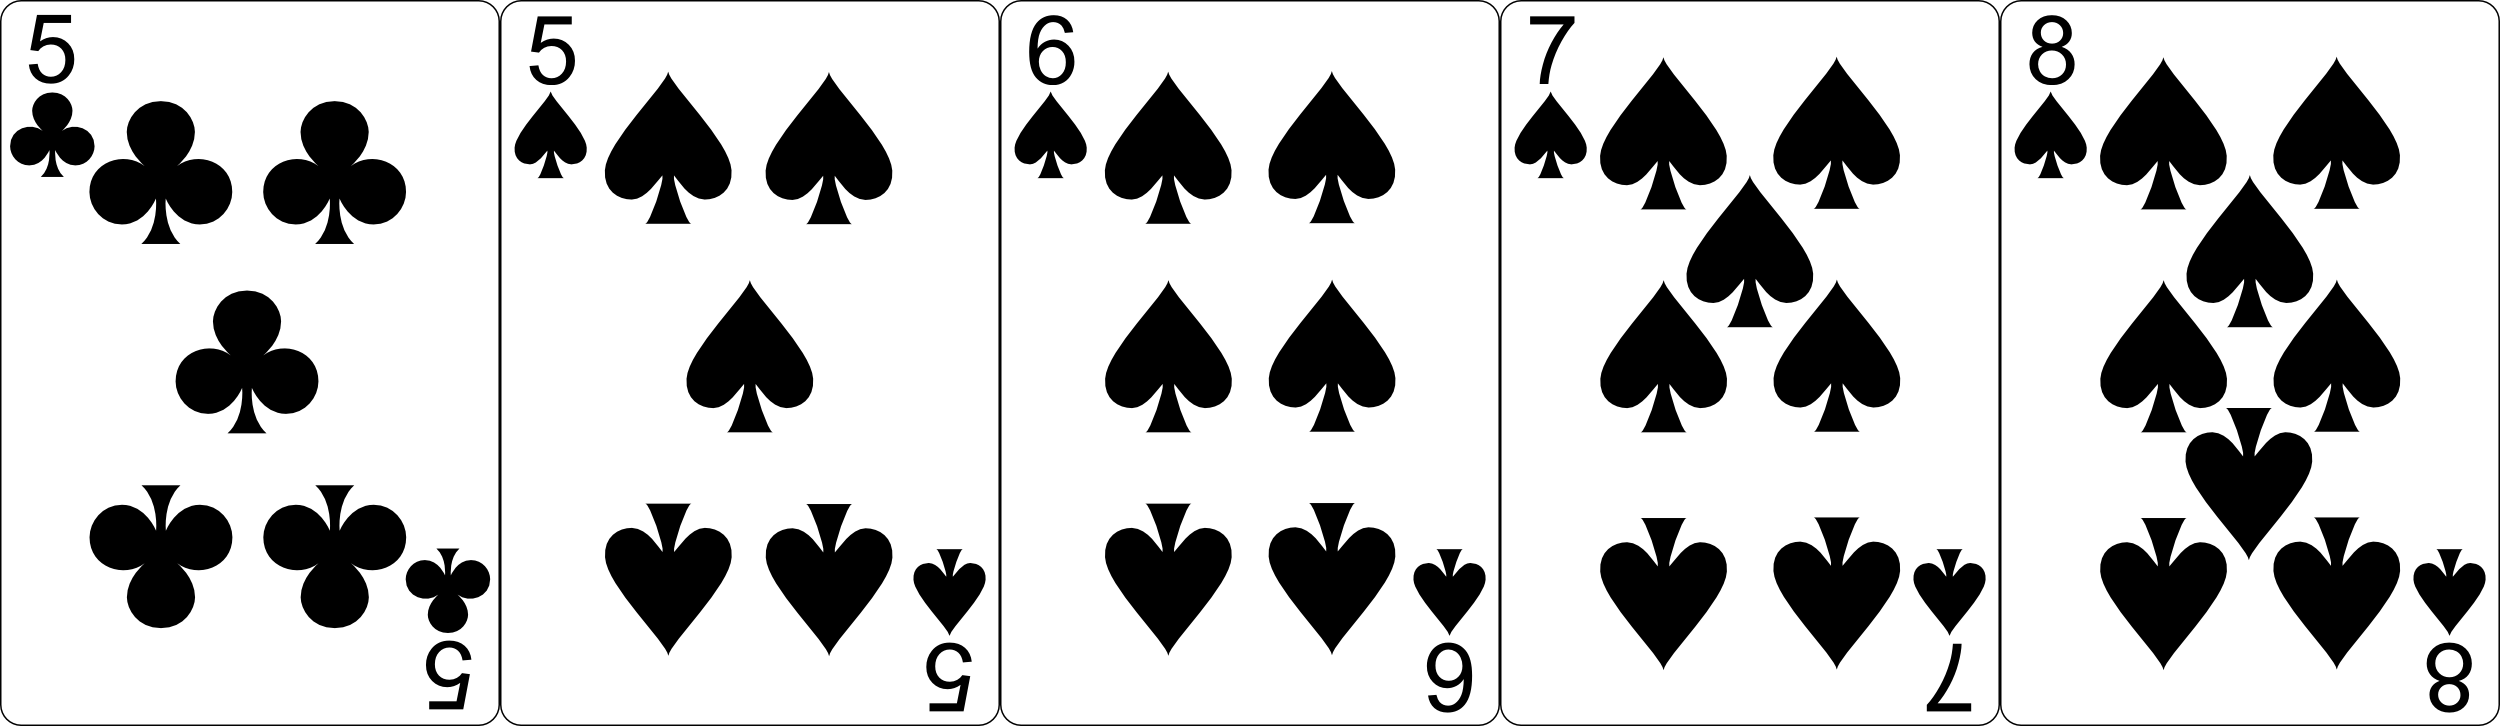
\includegraphics[width=\textwidth]{../img/w05-hands/pair.png}
 \end{minipage}
 \begin{minipage}[c]{\CardCaptionWidth}
  \caption{Par: två kort har samma valör.}
   \label{lab:shuffle:first-picture}
 \end{minipage}
\end{figure}

\begin{figure}[H]
 \begin{minipage}[c]{\CardWidth}
  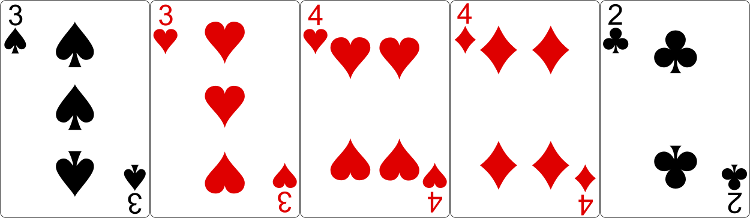
\includegraphics[width=\textwidth]{../img/w05-hands/twopair.png}
 \end{minipage}
 \begin{minipage}[c]{\CardCaptionWidth}
  \caption{Två par: handen har två \emph{olika} par.}
 \end{minipage}
\end{figure}

\begin{figure}[H]
 \begin{minipage}[c]{\CardWidth}
  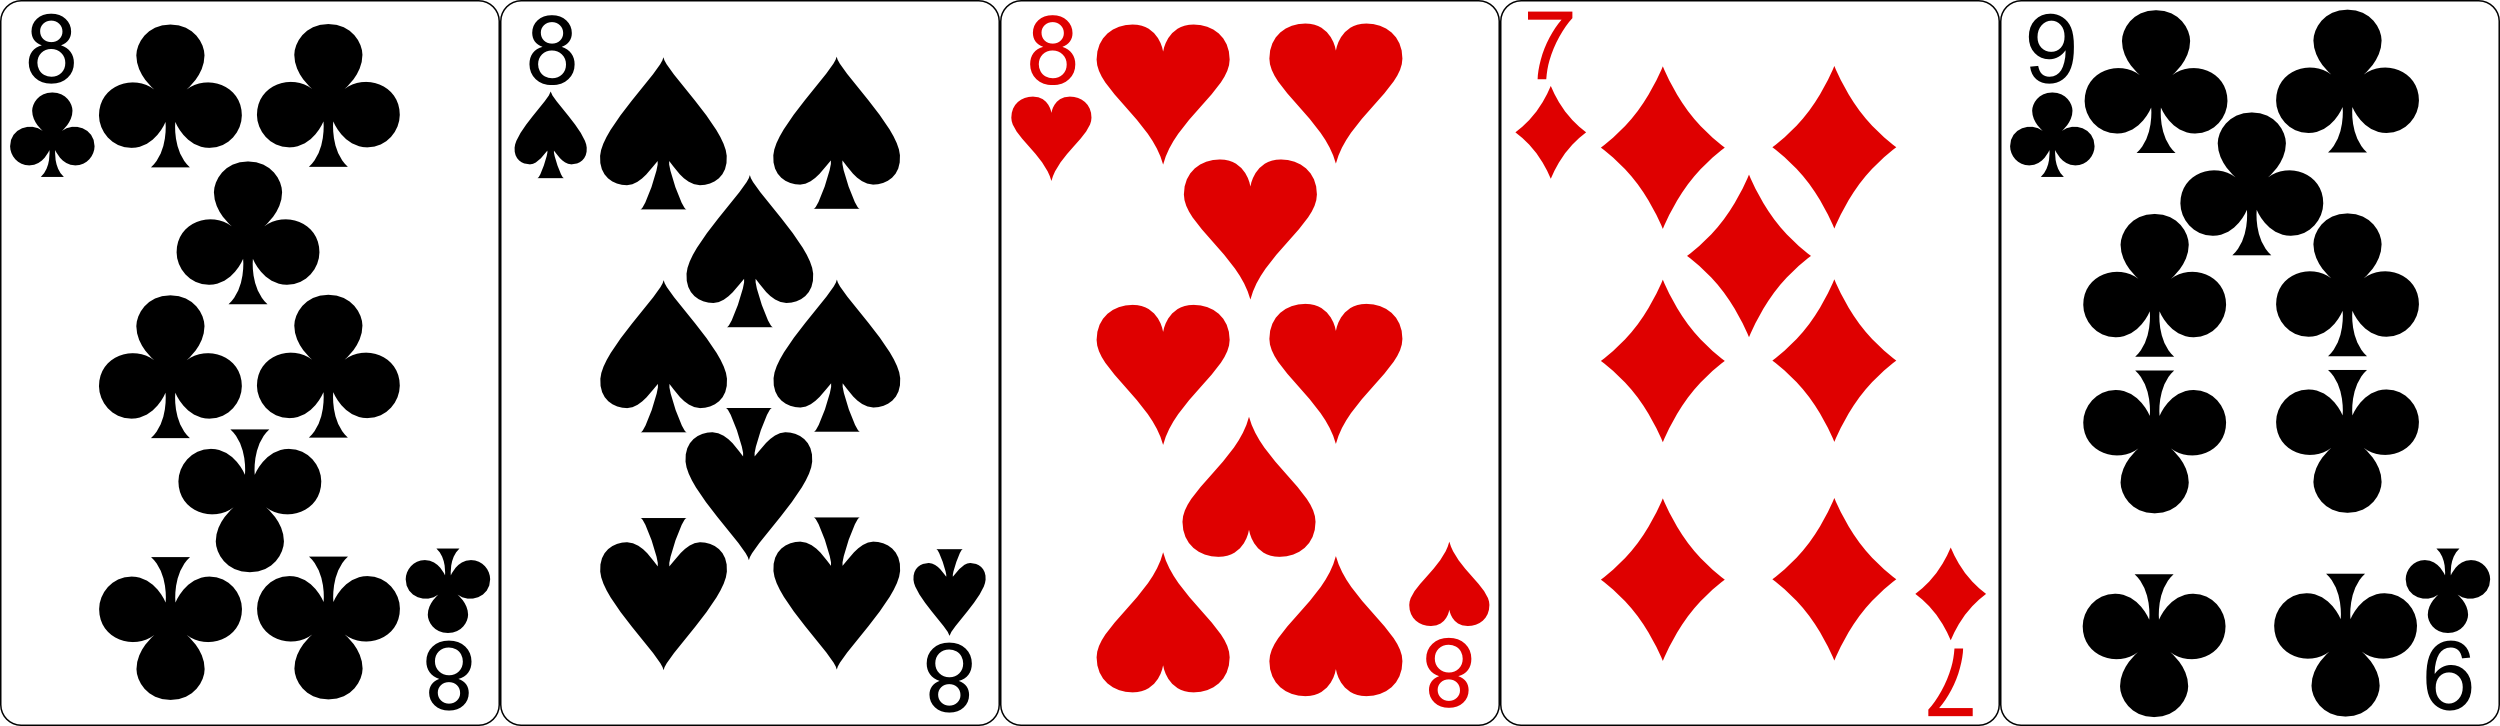
\includegraphics[width=\textwidth]{../img/w05-hands/trips.png}
 \end{minipage}
 \begin{minipage}[c]{\CardCaptionWidth}
  \caption{Triss: tre kort har samma valör.}
 \end{minipage}
\end{figure}

\begin{figure}[H]
 \begin{minipage}[c]{\CardWidth}
  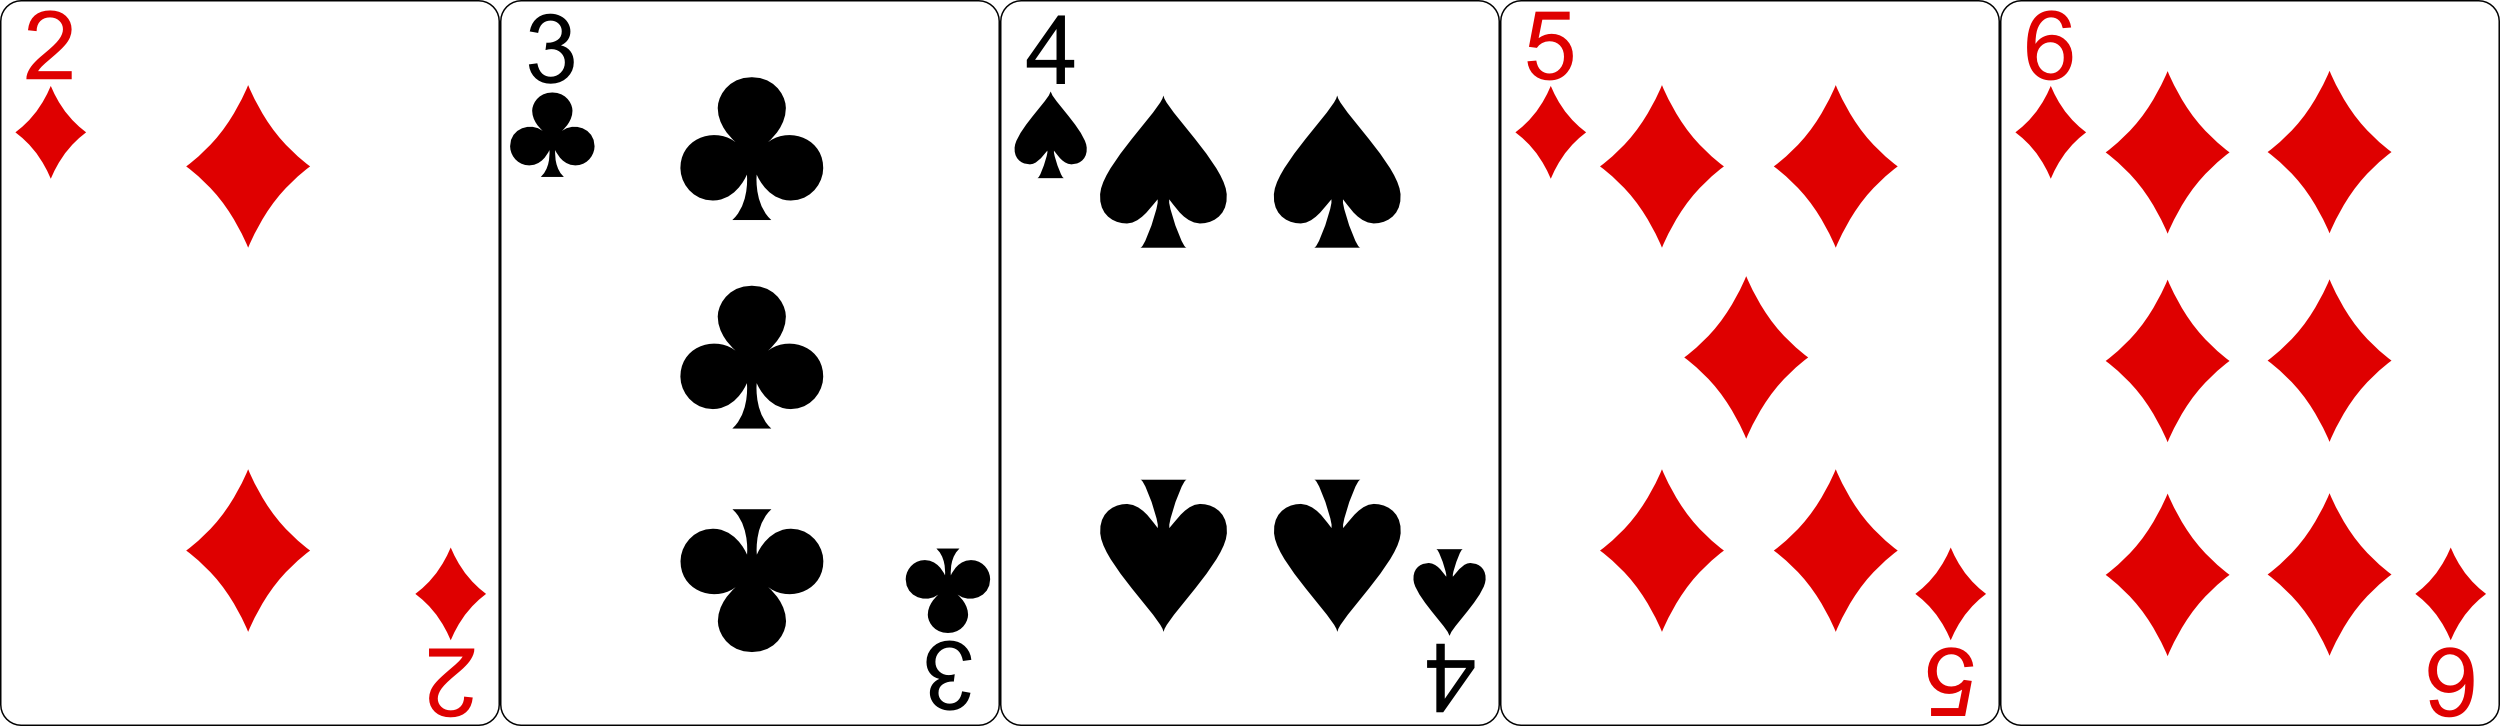
\includegraphics[width=\textwidth]{../img/w05-hands/straight.png}
 \end{minipage}
 \begin{minipage}[c]{\CardCaptionWidth}
  \caption{Stege: kortens valörer bildar en följd, ess kan vara antingen 1 eller 14.}
 \end{minipage}
\end{figure}

\begin{figure}[H]
 \begin{minipage}[c]{\CardWidth}
  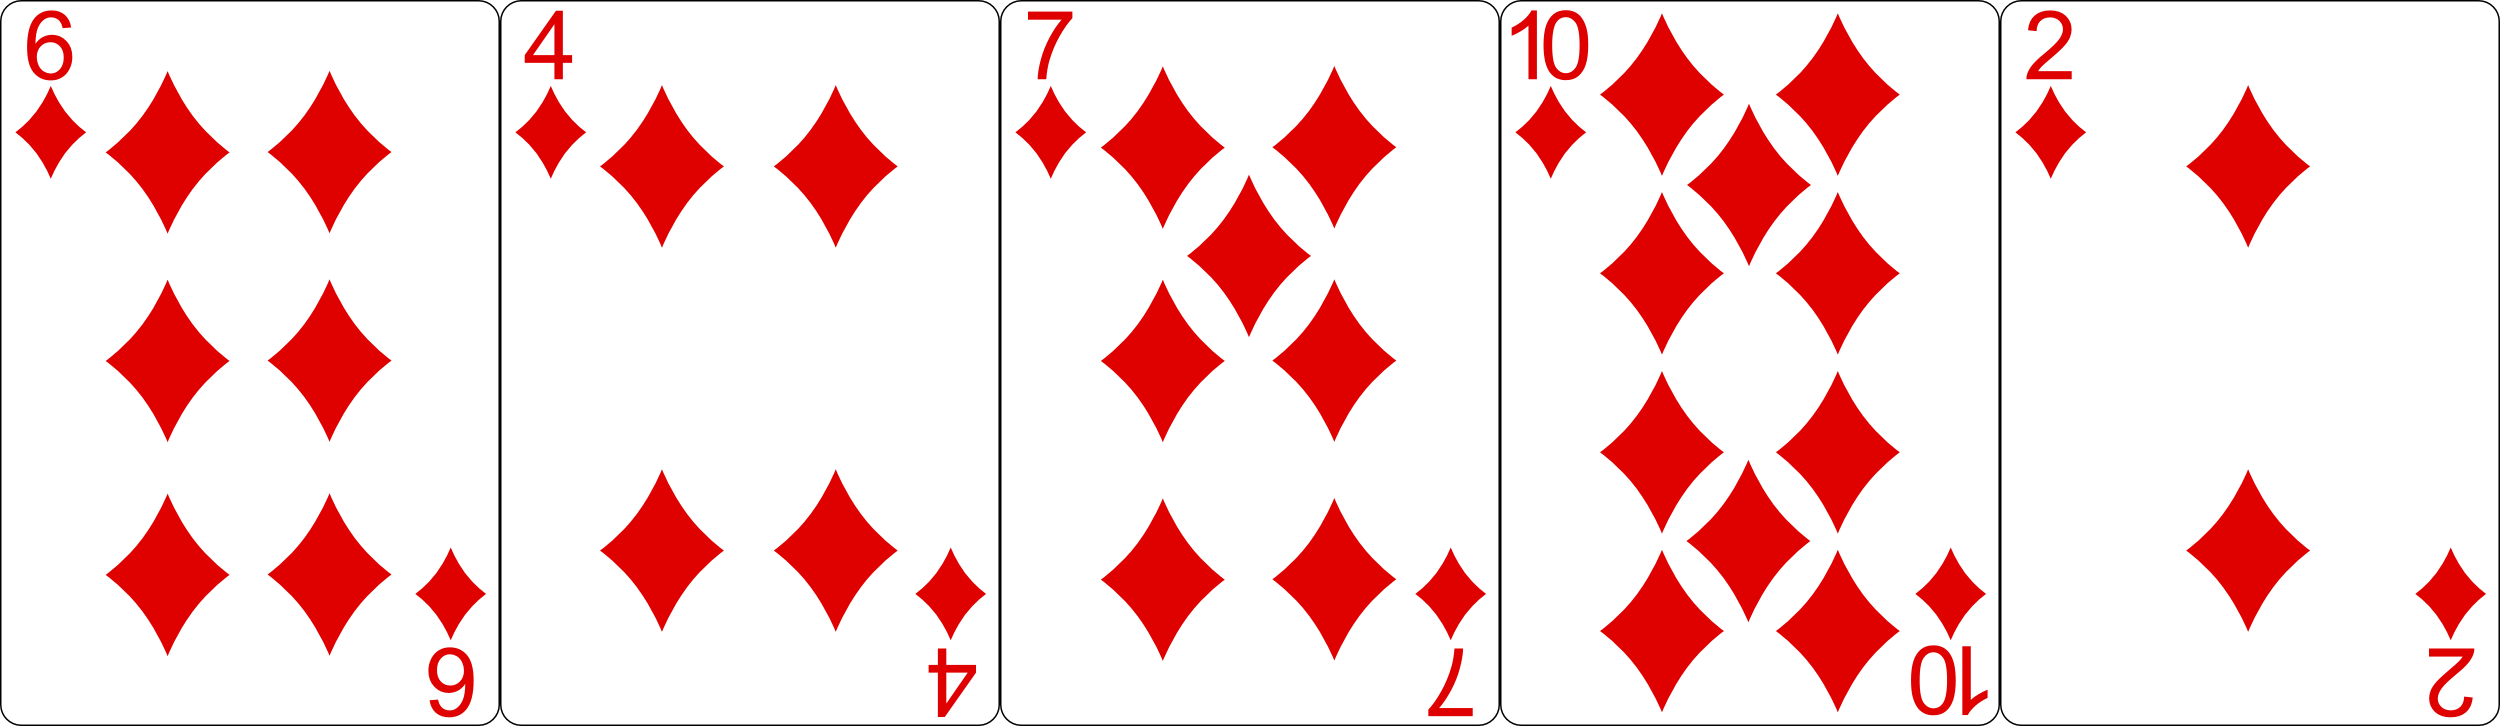
\includegraphics[width=\textwidth]{../img/w05-hands/flush.png}
 \end{minipage}
 \begin{minipage}[c]{\CardCaptionWidth}
  \caption{Färg: alla kort har samma färg.}
 \end{minipage}
\end{figure}

\begin{figure}[H]
 \begin{minipage}[c]{\CardWidth}
  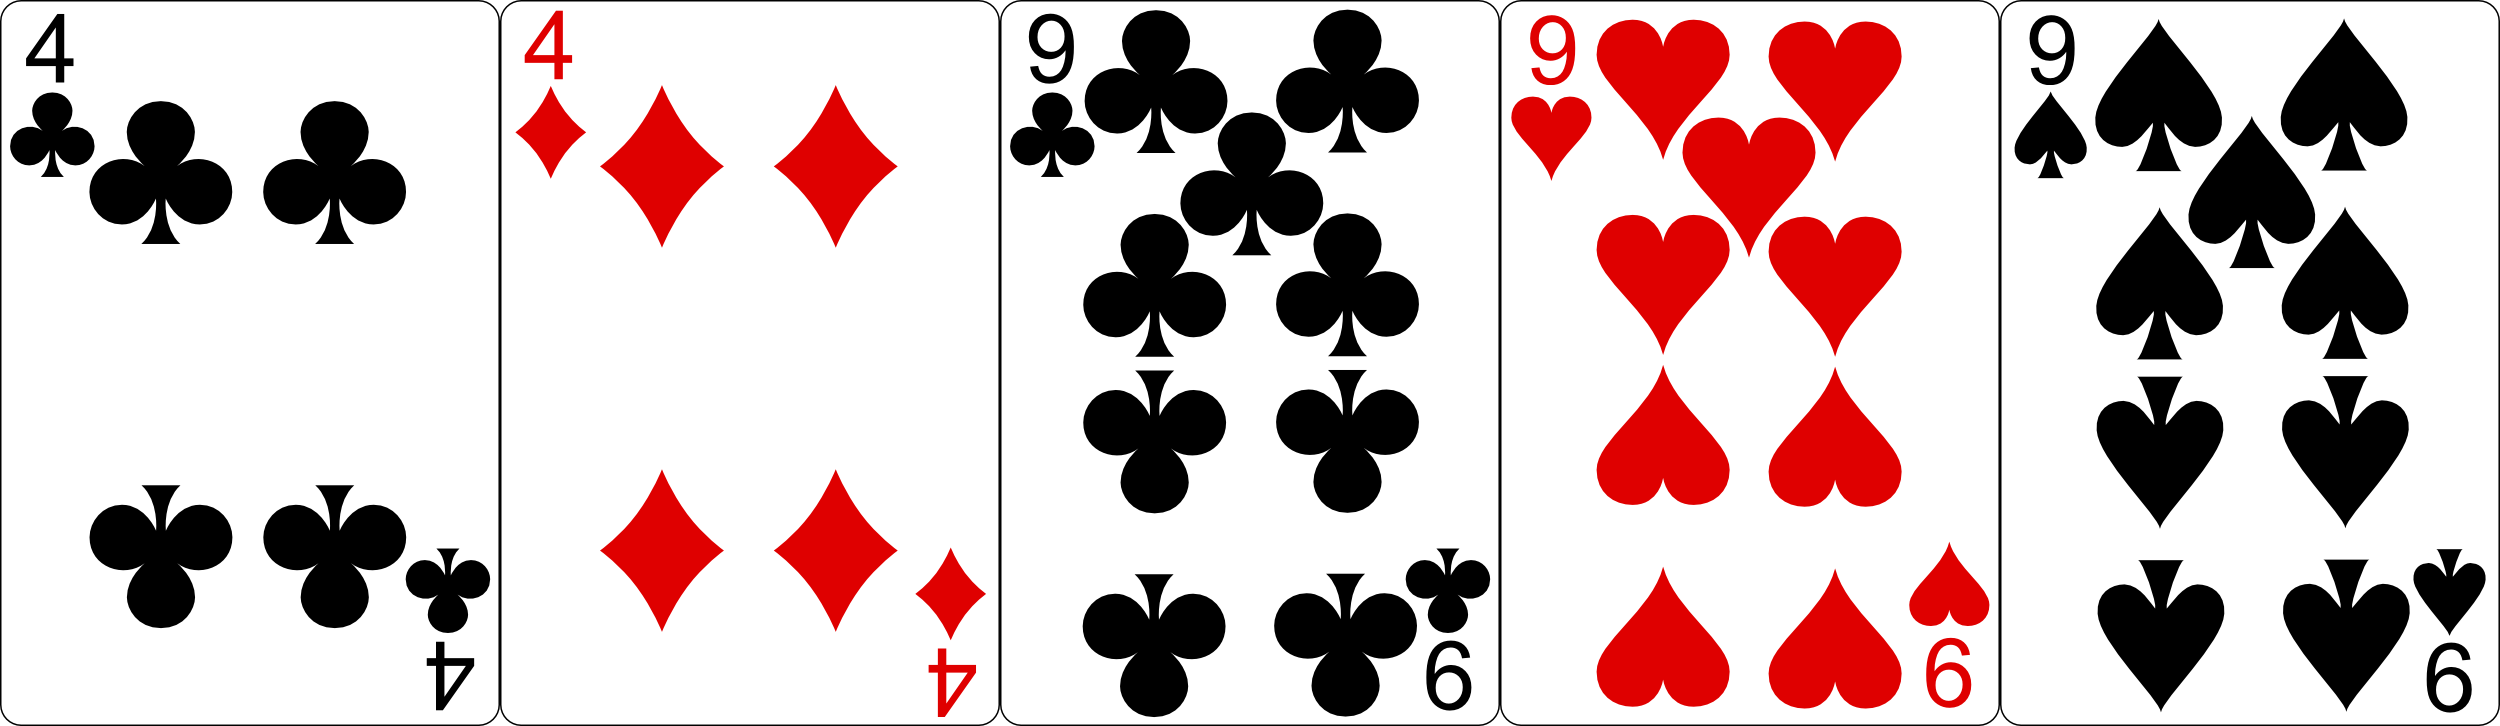
\includegraphics[width=\textwidth]{../img/w05-hands/fullhouse.png}
 \end{minipage}
 \begin{minipage}[c]{\CardCaptionWidth}
  \caption{Kåk: både triss och par.}
 \end{minipage}
\end{figure}

\begin{figure}[H]
 \begin{minipage}[c]{\CardWidth}
  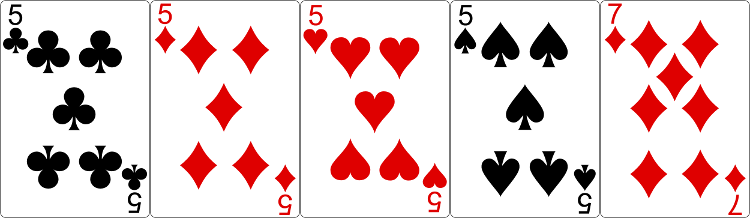
\includegraphics[width=\textwidth]{../img/w05-hands/fours.png}
 \end{minipage}
 \begin{minipage}[c]{\CardCaptionWidth}
  \caption{Fyrtal: fyra kort har samma valör.}
 \end{minipage}
\end{figure}

\begin{figure}[H]
 \begin{minipage}[c]{\CardWidth}
  \includegraphics[width=\textwidth]{../img/w05-hands/straightflush.png}
 \end{minipage}
 \begin{minipage}[c]{\CardCaptionWidth}
  \caption{Färgstege: både stege och färg.}
 \end{minipage}
\end{figure}

\begin{figure}[H]
 \begin{minipage}[c]{\CardWidth}
  \includegraphics[width=\textwidth]{../img/w05-hands/none.png}
 \end{minipage}
 \begin{minipage}[c]{\CardCaptionWidth}
  \caption{Högt kort: inget mönster finns.}
 \label{lab:shuffle:last-picture}
  \end{minipage}
\end{figure}


%!TEX encoding = UTF-8 Unicode

%!TEX root = ../compendium1.tex

%!TEX encoding = UTF-8 Unicode
\chapter{Matriser, typparametrar}\label{chapter:W08}
Begrepp som ingår i denna veckas studier:
\begin{itemize}[noitemsep,label={$\square$},leftmargin=*]
\item matris
\item nästlad samling
\item nästlad for-sats
\item typparameter
\item generisk funktion
\item generisk klass
\item fri vs bunden typparameter
\item generiska datastrukturer
\item generiska samlingar i Scala\end{itemize}

\clearpage\section{Teori}
%!TEX encoding = UTF-8 Unicode
%!TEX root = ../lect-w08.tex

%%%

\Subsection{Veckans labb: \texttt{life}}

\begin{Slide}{Veckans labb: \texttt{life}}
\begin{minipage}{0.52\textwidth}
  \setlength{\leftmargini}{0pt}

\begin{itemize}
  \SlideFontSmall
\item Universum är en binär matris av \Emph{celler} där \Emph{levande} celler representeras med \code{true} och \Alert{döda} med \code{false}.
\item Följande regler gäller för \Emph{nästa generation} celler i universum:
\begin{itemize}\SlideFontTiny
  \item \textbf{Fortlevnad}: en levande cell med 2 eller 3 grannar \Emph{lever vidare}
  \item \textbf{Död}: en levande cell med färre än 2 eller fler än 3 grannar \Alert{dör}
  \item \textbf{Födelse}: en död cell med exakt tre grannar föds
\end{itemize}
\item Övning \code{matrices} uppgift 5: skapa en generisk \code{case class Matrix[T]}
\item På labben: använd \code{Matrix[Boolean]}
\end{itemize}

\end{minipage}%
\begin{minipage}{0.5\textwidth}
  \includegraphics[width=1.0\textwidth]{../img/glider-blinker-block}

  \begin{itemize}\SlideFontTiny
  \item Du ska simulera \emph{Game of Life} i ett \code{introprog.PixelWindow}
  \item Fördjupning:\\{\SlideFontTiny\url{https://en.wikipedia.org/wiki/Conway%27s_Game_of_Life}}
  \end{itemize}
\end{minipage}%

\end{Slide}






\Subsection{Matriser}

\begin{Slide}{Vad är en matris?}\SlideFontSmall
\begin{itemize}

\item En \Emph{matris} inom \Alert{matematiken} innehåller \Emph{rader} och \Emph{kolumner}\footnote{även kallade \emph{kolonner}} med tal.

\item I en \Alert{matematisk} matris har alla rader \Emph{lika många} element och

\item även alla kolumner har \Emph{lika många} element.

\item En matris av dimension $2\times{}5$ har $2 \cdot 5 = 10$ stycken element.

\item Exempel på en matematisk matris av dimension $2\times{}5$:
\[
M_{2,5}=
  \begin{pmatrix}
    5 & 2 & 42 & 4 & 5 \\
    3 & 4 & 18 & 6 & 7
  \end{pmatrix}
\]
\end{itemize}
\end{Slide}

\begin{Slide}{Indexering i en matris}\SlideFontSmall
\begin{itemize}

  \item En matris av dimension $m\times{}n$ har $m \cdot n$ stycken element.

  \item En matris $A_{m,n}$ av dimension $m\times{}n$ ritas inom matematiken ofta så här:

  \[
  A_{m,n} =
   \begin{pmatrix}
    a_{1,1} & a_{1,2} & \cdots & a_{1,n} \\
    a_{2,1} & a_{2,2} & \cdots & a_{2,n} \\
    \vdots  & \vdots  & \ddots & \vdots  \\
    a_{m,1} & a_{m,2} & \cdots & a_{m,n}
   \end{pmatrix}
  \]


\item Matrisindexering inom matematiken sker ofta från $1$, men ofta från $0$ i datorprogram.

\item Vad har talet $42$ för index i matrisen $M_{2,5}$ nedan?
\begin{itemize}\SlideFontTiny
  \item[--] Inom matematiken?
  \item[--] I Scala och Java och många andra språk?

  \[
  M_{2,5}=
    \begin{pmatrix}
      5 & 2 & 42 & 4 & 5 \\
      3 & 4 & 18 & 6 & 7
    \end{pmatrix}
  \]
\end{itemize}
\end{itemize}
\end{Slide}

\begin{Slide}{En matris med array av arrayer}
Inom programmering används ordet \Emph{matris} ofta för att beteckna en \Alert{nästlad struktur} i två dimensioner, till exempel en instans av typen \code{Array[Array[Int]]}
\begin{REPL}
scala> val xss = Array(Array(5,2,42,4,5),Array(3,4,18,6,7))
xss: Array[Array[Int]] = Array(Array(5, 2, 42, 4, 5), Array(3, 4, 18, 6, 7))
\end{REPL}
\pause
Man indexerar i en nästlad sekvens med upprepad \code{apply}:
\begin{REPL}
scala> xss(0)(2)
res0: ???                   // Vad är typ och värde?

scala> xss.apply(0).apply(2)
res1: ???                   // Vad är typ och värde?

scala> xss(0)
res2: ???                   // Vad är typ och värde?
\end{REPL}

\end{Slide}

\begin{Slide}{En matris med array av arrayer}
Inom programmering används ordet \Emph{matris} ofta för att beteckna en \Alert{nästlad struktur} i två dimensioner, till exempel en instans av typen \code{Array[Array[Int]]}
\begin{REPL}
scala> val xss = Array(Array(5,2,42,4,5),Array(3,4,18,6,7))
xss: Array[Array[Int]] = Array(Array(5, 2, 42, 4, 5), Array(3, 4, 18, 6, 7))
\end{REPL}

Man indexerar i en nästlad sekvens med upprepad \code{apply}:
\begin{REPL}
scala> xss(0)(2)
res0: Int = 42

scala> xss.apply(0).apply(2)
res1: Int = 42

scala> xss(0)
res2: Array[Int] = Array(5, 2, 42, 4, 5)
\end{REPL}
\end{Slide}

\begin{Slide}{Uppdatering av en förändringsbar nästlad struktur}
Man kan förändra en array av arrayer ''på plats'' med tilldelning:
\begin{REPL}
scala> val xss = Array(Array(5,2,42,4,5),Array(3,4,18,6,7))

scala> xss(0)(0) = 100

scala> xss
res0: ???

scala> xss(0)(2) = xss(0)(2) - 1

scala> xss
res1: ???

scala> xss(1) = Array.fill(5)(-1)

scala> xss
res2: ???
\end{REPL}
\end{Slide}

\begin{Slide}{Uppdatering av en förändringsbar nästlad struktur}
Man kan förändra en array av arrayer ''på plats'' med tilldelning:
\begin{REPL}
scala> val xss = Array(Array(5,2,42,4,5),Array(3,4,18,6,7))

scala> xss(0)(0) = 100

scala> xss
res0: Array[Array[Int]]=Array(Array(100, 2, 42, 4, 5), Array(3, 4, 18, 6, 7))

scala> xss(0)(2) = xss(0)(2) - 1

scala> xss
res1: Array[Array[Int]]=Array(Array(100, 2, 41, 4, 5), Array(3, 4, 18, 6, 7))

scala> xss(1) = Array.fill(5)(-1)

scala> xss
res2: Array[Array[Int]]=Array(Array(100, 2, 41, 4, 5), Array(-1,-1,-1,-1,-1))
\end{REPL}
\end{Slide}

\begin{Slide}{Några olika sätt att skapa förändringsbara matriser}\SlideFontSmall
Det jobbiga, primitiva sättet:
\begin{REPL}
scala> val xs = new Array[Array[Int]](2)
xs: Array[Array[Int]] = Array(null, null)

scala> for (i <- xs.indices) {xs(i) = new Array[Int](5)}

scala> xs
res0: Array[Array[Int]] = Array(Array(0, 0, 0, 0, 0), Array(0, 0, 0, 0, 0))

scala> println(xs)
[[I@196a99d0
\end{REPL}
Enklare sätt:
\begin{REPL}
scala> val xs = Array.ofDim[Int](2,5)
xs: Array[Array[Int]] = Array(Array(0, 0, 0, 0, 0), Array(0, 0, 0, 0, 0))
\end{REPL}
Enklare och tydligare sätt, där initialvärdet anges explicit:
\begin{REPL}
scala> Array.fill(2,5)(0)
res37: Array[Array[Int]] = Array(Array(0, 0, 0, 0, 0), Array(0, 0, 0, 0, 0))
\end{REPL}

\end{Slide}

\begin{Slide}{Exempel på skapande av oföränderlig nästlad struktur}\SlideFontSmall
Om du kan beräkna initialvärde direkt, använd \code{Vector.fill}:\\
{\SlideFontTiny\code{def fill[A](n1: Int, n2: Int)(elem: => A): Vector[Vector[A]]}}
\begin{REPL}
scala> Vector.fill(2,5)(scala.util.Random.nextInt(6) + 1)
res0:
  typ???
  värde???

\end{REPL}
Om du kan beräkna initialvärde ur index, använd \code{Vector.tabulate}:\\
{\SlideFontTiny\code{def tabulate[A](n1: Int, n2: Int)(f: (Int, Int) => A): Vector[Vector[A]]}}
\begin{REPL}
scala> Vector.tabulate(5,2)((x,y) => x + y + 1)
res1:
  typ???
  värde???

\end{REPL}
\end{Slide}

\begin{Slide}{Exempel på skapande av oföränderlig nästlad struktur}\SlideFontSmall
Om du kan beräkna initialvärde direkt, använd \code{Vector.fill}:\\
{\SlideFontTiny\code{def fill[A](n1: Int, n2: Int)(elem: => A): Vector[Vector[A]]}}
\begin{REPL}
scala> Vector.fill(2,5)(scala.util.Random.nextInt(6) + 1)
res0:
  scala.collection.immutable.Vector[scala.collection.immutable.Vector[Int]] =
  Vector(Vector(1, 2, 6, 2, 1), Vector(1, 4, 3, 3, 2))

\end{REPL}
Om du kan beräkna initialvärde ur index, använd \code{Vector.tabulate}:\\
{\SlideFontTiny\code{def tabulate[A](n1: Int, n2: Int)(f: (Int, Int) => A): Vector[Vector[A]]}}
\begin{REPL}
scala> Vector.tabulate(5,2)((x,y) => x + y + 1)
res1:
  scala.collection.immutable.Vector[scala.collection.immutable.Vector[Int]] =
  Vector(Vector(1,2), Vector(2,3), Vector(3,4), Vector(4,5), Vector(5,	6))

\end{REPL}
\end{Slide}



\begin{Slide}{Uppdatering av en oföränderlig nästlad struktur}\SlideFontSmall
Uppdatering av endimensionell struktur med \code{xs.updated}:\\
{\SlideFontTiny\code{def updated[A](index: Int, elem: A): Vector[A]} }
\begin{REPL}
scala> var xs = Vector.tabulate(5)(x => x + 1)
xs: typ??? = värde???

scala> xs = xs.updated(1, 42)
xs: typ??? = värde???
\end{REPL}

Uppdatering av nästlad struktur i två dimensioner:
\begin{REPL}
scala> var xss = Vector.tabulate(2, 5)((x,y) => x + y + 1)
xss:
  typ??? =
  värde???

scala> xss = xss.updated(0, xss(0).updated(1, 42))
xss:
  typ??? =
  värde???
\end{REPL}

\end{Slide}



\begin{Slide}{Uppdatering av en oföränderlig nästlad struktur}\SlideFontSmall
Uppdatering av endimensionell struktur med \code{xs.updated}:\\
{\SlideFontTiny\code{def updated[A](index: Int, elem: A): Vector[A]} }
\begin{REPL}
scala> var xs = Vector.tabulate(5)(x => x + 1)
xs: scala.collection.immutable.Vector[Int] = Vector(1, 2, 3, 4, 5)

scala> xs = xs.updated(1, 42)
xs: scala.collection.immutable.Vector[Int] = Vector(1, 42, 3, 4, 5)
\end{REPL}

Uppdatering av nästlad struktur i två dimensioner:
\begin{REPL}
scala> var xss = Vector.tabulate(2, 5)((x,y) => x + y + 1)
xss:
  scala.collection.immutable.Vector[scala.collection.immutable.Vector[Int]] =
  Vector(Vector(1, 2, 3, 4, 5), Vector(2, 3, 4, 5, 6))

scala> xss = xss.updated(0, xss(0).updated(1, 42))
xss:
  scala.collection.immutable.Vector[scala.collection.immutable.Vector[Int]] =
  Vector(Vector(1, 42, 3, 4, 5), Vector(2, 3, 4, 5, 6))
\end{REPL}

\end{Slide}


\begin{Slide}{Iterera över nästlad struktur: for-sats}\SlideFontSmall
Iterera med nästlad for-sats:
\begin{REPL}
scala> val xss = Vector.tabulate(2,5)((x,y) => x + y + 1)

scala> for (???) {
         for (???) {
           print(xss(i)(j) + " ")
         }
         println
       }

1 2 3 4 5
2 3 4 5 6
\end{REPL}
\end{Slide}

\begin{Slide}{Iterera över nästlad struktur: for-sats}\SlideFontSmall
Iterera med nästlad for-sats:
\begin{REPL}
scala> val xss = Vector.tabulate(2,5)((x,y) => x + y + 1)

scala> for (i <- xss.indices) {
         for (j <- xss(i).indices) {
           print(xss(i)(j) + " ")
         }
         println
       }

1 2 3 4 5
2 3 4 5 6
\end{REPL}
\end{Slide}


\begin{Slide}{Övningsexempel: Yatzy}\SlideFontSmall
Skapa en funktion \code{roll} som ger utfallet av n st tärningskast:
\begin{REPL}
scala> import scala.util.Random

scala> def roll(n: Int): Vector[Int] = ???
\end{REPL}

Skapa en funktion \code{isYatzy} som ger \code{true} om alla utfall är lika:
\begin{REPL}
scala> def isYatzy(xs: Vector[Int]): Boolean = ???
\end{REPL}
Du kan anta att xs.length > 0\\
Tips: använd metoden xs.forall: \\
\code{def forall[A](p: A => Boolean): Boolean }
\end{Slide}


\begin{Slide}{Övningsexempel: Yatzy}\SlideFontSmall
Skapa en funktion \code{roll} som ger utfallet av n st tärningskast:
\begin{REPL}
scala> import scala.util.Random

scala> def roll(n: Int): Vector[Int] = Vector.fill(n)(Random.nextInt(6) + 1)
\end{REPL}

Skapa en funktion \code{isYatzy} som ger \code{true} om alla utfall är lika:
\begin{REPL}
scala> def isYatzy(xs: Vector[Int]): Boolean = xs.forall(x => x == xs(0))
\end{REPL}
Du kan anta att xs.length > 0\\
Tips: använd metoden xs.forall: \\
\code{def forall[A](p: A => Boolean): Boolean }
\end{Slide}

\begin{Slide}{Iterera över nästlad struktur: for-sats}\SlideFontSmall
Iterera med nästlad for-sats: (vad har xss för typ?)
\begin{REPL}
scala> val xss = Vector.fill(100)(roll(5))

scala> for (???) {
         for (???) {
           print(s"($i)($j) == " + xss(i)(j) + " ")
         }
         println(isYatzy(???))
       }

(0)(0) == 5 (0)(1) == 3 (0)(2) == 4 (0)(3) == 1 (0)(4) == 3 false
(1)(0) == 3 (1)(1) == 3 (1)(2) == 6 (1)(3) == 3 (1)(4) == 1 false
(2)(0) == 3 (2)(1) == 4 (2)(2) == 2 (2)(3) == 2 (2)(4) == 1 false
(3)(0) == 5 (3)(1) == 2 (3)(2) == 6 (3)(3) == 5 (3)(4) == 1 false
(4)(0) == 4 (4)(1) == 6 (4)(2) == 4 (4)(3) == 1 (4)(4) == 4 false
(5)(0) == 3 (5)(1) == 4 (5)(2) == 6 (5)(3) == 5 (5)(4) == 1 false
(6)(0) == 4 (6)(1) == 6 (6)(2) == 2 (6)(3) == 2 (6)(4) == 6 false
(7)(0) == 2 (7)(1) == 5 (7)(2) == 3 (7)(3) == 6 (7)(4) == 2 false
(8)(0) == 4 (8)(1) == 4 (8)(2) == 6 (8)(3) == 1 (8)(4) == 4 false
(9)(0) == 3 (9)(1) == 3 (9)(2) == 3 (9)(3) == 3 (9)(4) == 3 true
(10)(0) == 1 (10)(1) == 2 (10)(2) == 4 (10)(3) == 3 (10)(4) == 3 false
(11)(0) == 6 (11)(1) == 5 (11)(2) == 4 (11)(3) == 1 (11)(4) == 5 false
(12)(0) == 3 (12)(1) == 6 (12)(2) == 6 (12)(3) == 4 (12)(4) == 2 false
\end{REPL}
\end{Slide}

\begin{Slide}{Iterera över nästlad struktur: for-sats}\SlideFontSmall
Iterera med nästlad for-sats: (xss är en \code{Vector[Vector[Int]]})
\begin{REPL}
scala> val xss = Vector.fill(100)(roll(5))

scala> for (i <- xss.indices) {
         for (j <- xss(i).indices) {
           print(s"($i)($j) == " + xss(i)(j) + " ")
         }
         println(isYatzy(xss(i)))
       }

(0)(0) == 5 (0)(1) == 3 (0)(2) == 4 (0)(3) == 1 (0)(4) == 3 false
(1)(0) == 3 (1)(1) == 3 (1)(2) == 6 (1)(3) == 3 (1)(4) == 1 false
(2)(0) == 3 (2)(1) == 4 (2)(2) == 2 (2)(3) == 2 (2)(4) == 1 false
(3)(0) == 5 (3)(1) == 2 (3)(2) == 6 (3)(3) == 5 (3)(4) == 1 false
(4)(0) == 4 (4)(1) == 6 (4)(2) == 4 (4)(3) == 1 (4)(4) == 4 false
(5)(0) == 3 (5)(1) == 4 (5)(2) == 6 (5)(3) == 5 (5)(4) == 1 false
(6)(0) == 4 (6)(1) == 6 (6)(2) == 2 (6)(3) == 2 (6)(4) == 6 false
(7)(0) == 2 (7)(1) == 5 (7)(2) == 3 (7)(3) == 6 (7)(4) == 2 false
(8)(0) == 4 (8)(1) == 4 (8)(2) == 6 (8)(3) == 1 (8)(4) == 4 false
(9)(0) == 3 (9)(1) == 3 (9)(2) == 3 (9)(3) == 3 (9)(4) == 3 true
(10)(0) == 1 (10)(1) == 2 (10)(2) == 4 (10)(3) == 3 (10)(4) == 3 false
(11)(0) == 6 (11)(1) == 5 (11)(2) == 4 (11)(3) == 1 (11)(4) == 5 false
(12)(0) == 3 (12)(1) == 6 (12)(2) == 6 (12)(3) == 4 (12)(4) == 2 false
\end{REPL}
\end{Slide}


\begin{Slide}{Iterera över nästlad struktur med nästlad foreach}\SlideFontSmall
Iterera med nästlad foreach-sats:
\begin{REPL}
scala> val xss = Vector.tabulate(2,5)((x,y) => x + y + 1)

xss.foreach{ xs => ??? ; println }

1 2 3 4 5
2 3 4 5 6
\end{REPL}
\end{Slide}


\begin{Slide}{Iterera över nästlad struktur med nästlad foreach}\SlideFontSmall
Iterera med nästlad foreach-sats:
\begin{REPL}
scala> val xss = Vector.tabulate(2,5)((x,y) => x + y + 1)

xss.foreach{ xs => xs.foreach{ x => print(x + " ") }; println }

1 2 3 4 5
2 3 4 5 6
\end{REPL}
\end{Slide}


\begin{Slide}{Nästlade for-uttryck}\SlideFontSmall
Iterera med \Emph{nästlad for-yield}:\\
%Statisk typ: \code{IndexedSeq[IndexedSeq[[Int]]} \\
%Dynamisk typ: \code{Vector[Vector[[Int]]}

\begin{REPL}
scala> val xss = for (i <- 1 to 2) yield {
                   for (j <- 1 to 5) yield i + j + 1
                 }
xss:
  scala.collection.immutable.IndexedSeq[
    scala.collection.immutable.IndexedSeq[Int]] =
      ???

\end{REPL}
Om man skriver så här får man en endimensionell struktur:
\begin{REPL}
scala> val xs = for (i <- 1 to 2; j <- 1 to 5) yield i + j + 1
xs:
  scala.collection.immutable.IndexedSeq[Int] =
    ???

\end{REPL}
\end{Slide}

\begin{Slide}{Nästlade for-uttryck}\SlideFontSmall
Iterera med \Emph{nästlad for-yield}:\\
\begin{REPL}
scala> val xss = for (i <- 1 to 2) yield {
                   for (j <- 1 to 5) yield i + j + 1
                 }
xss:
  scala.collection.immutable.IndexedSeq[
    scala.collection.immutable.IndexedSeq[Int]] =
      Vector(Vector(3, 4, 5, 6, 7), Vector(4, 5, 6, 7, 8))

\end{REPL}
Om man skriver så här får man en endimensionell struktur:
\begin{REPL}
scala> val xs = for (i <- 1 to 2; j <- 1 to 5) yield i + j + 1
xs:
  scala.collection.immutable.IndexedSeq[Int] =
    Vector(3, 4, 5, 6, 7, 4, 5, 6, 7, 8)

\end{REPL}
\end{Slide}



\begin{Slide}{Nästlade map-uttryck}\SlideFontSmall
Iterera med \Emph{nästlade map-uttryck}:\\
\begin{REPL}
scala> val xss = (1 to 2).map(i => (1 to 5).map(j => i + j + 1))
xss:
  scala.collection.immutable.IndexedSeq[
    scala.collection.immutable.IndexedSeq[Int]] =
      ???
\end{REPL}
\end{Slide}

\begin{Slide}{Nästlade map-uttryck}\SlideFontSmall
Iterera med \Emph{nästlade map-uttryck}:\\
\begin{REPL}
scala> val xss = (1 to 2).map(i => (1 to 5).map(j => i + j + 1))
xss:
  scala.collection.immutable.IndexedSeq[
    scala.collection.immutable.IndexedSeq[Int]] =
      Vector(Vector(3, 4, 5, 6, 7), Vector(4, 5, 6, 7, 8))
\end{REPL}
\end{Slide}




\begin{Slide}{Matris som Array med Array med heltal i Java}\SlideFontTiny
\begin{CodeSmall}[language=Java]
public class ArrayMatrix {

    public static void showMatrix(int[][] m){
        System.out.println("\n--- showMatrix ---");
        for (int row = 0; row < m.length; row++){
            for (int col = 0; col < m[row].length; col++) {
                System.out.print("[" + row + "]");
                System.out.print("[" + col + "] = ");
                System.out.print(m[row][col] + "; ");
            }
            System.out.println();
        }
    }

    public static void main(String[] args) {
        int[][] xss = new int[10][5];
        showMatrix(xss);
    }
}
\end{CodeSmall}
\pause
Övning: skriv en metod \code{fillRnd} som fyller en heltalsmatris med slumptal 1 till n:
\pause
\jcode|public static void fillRnd(int[][] m, int n){ /* ??? */ }| \\
\pause
Tips: använd en nästlad for-sats och: \\
\jcode{(int) (Math.random * n + 1)   // (int) motsvarar Scalas asInstanceOf[Int]}

\end{Slide}

\begin{Slide}{Om veckans övningar}\SlideFontSmall
\begin{itemize}
\item Träna på att iterera i nästlade strukurer

\item Fortsätt jobba med Yatzy-exemplet

\item träna på att skapa \Emph{imperativa} algoritmer: \\
lös \code{isYatzy} med \code{while}-sats (kunde varit del av en tenta...)

\item Extrauppgift där du ska bygga ett enkelt yatzy-spel i terminalen (kunde varit en tentauppgift...)

\end{itemize}
\end{Slide}

% \begin{Slide}{Övning extrauppgift, utgör början på labb \code{survey}}\SlideFontSmall
%
% \begin{ScalaSpec}{Table}
% object Table {
%   /** Creates a new Table from fileName with columns split by sep */
%   def fromFile(fileName: String, separator: Char = ';'): Table = ???
% }
% case class Table(
%   data: Vector[Vector[String]],
%   headings: Vector[String],
%   sep: String){
%   /** A 2-tuple with (number of rows, number of columns) in data */
%   val dim: (Int, Int) = ???
%
%   /** The element in row r an column c of data, counting from 0 */
%   def apply(r: Int, c: Int): String = ???
%
%   /** The row-vector r in data, counting from 0 */
%   def row(r: Int): Vector[String]= ???
%
%   /** The column-vector c in data, counting from 0 */
%   def col(c: Int): Vector[String] = ???
%
%   /** A map from heading to index counting from 0 */
%   lazy val indexOfHeading: Map[String, Int] = ???
%
%   /** The column-vector with heading h in data */
%   def col(h: String): Vector[String] = ???
%
%   /** A vector with the distinct, sorted values of col with heading h */
%   def values(h: String): Vector[String] = ???
%
%   /** Headings and data with columns separated by sep */
%   override lazy val toString: String = ???
% }
% \end{ScalaSpec}
% \end{Slide}


% \begin{Slide}{Övn. fördjupn. uppg.: skapa en generisk matris-klass}\SlideFontSmall
% \vspace{-0.7em}
% \begin{Code}[basicstyle=\SlideFontSize{6}{6.8}\ttfamily\selectfont]
% case class Matrix[T](data: Vector[Vector[T]]){
%
%   def foreachRowCol(f: (Int, Int, T) => Unit): Unit =
%     for (r <- data.indices) {
%       for (c <- data(r).indices) {
%         f(r, c, data(r)(c))
%       }
%     }
%
%   def map[U](f: T => U): Matrix[U] = Matrix(data.map(_.map(f)))
%
%   /** The element at row r and column c */
%   def apply(r: Int, c: Int): T = ???
%
%   /** Gives Some[T](element) at index (r, c) if within index bounds, else None */
%   def get(r: Int, c: Int): Option[T] = ???
%
%   /** The row vector of row r */
%   def row(r: Int): Vector[T] = ???
%
%   /** The column vector of column c */
%   def col(c: Int): Vector[T] = ???
%
%   /** A new Matrix with element at row r and col c updated */
%   def updated(r: Int, c: Int, value: T): Matrix[T] = ???
% }
% object Matrix {
%   def fill[T](rowSize: Int, colSize: Int)(init: T): Matrix[T] =
%     new Matrix(Vector.fill(rowSize)(Vector.fill(colSize)(init)))
% }
% \end{Code}
% \end{Slide}

%!TEX encoding = UTF-8 Unicode
%!TEX root = ../lect-w08.tex

\Subsection{Typparametrar}



\begin{Slide}{Exempel: Icke-generisk case-klass med heltalsmatris}
  En \emph{icke-generisk} datastruktur har inga obundna typparametrar; alla typer är \Emph{konkreta} (alltså specifika). \\~\\ En icke-generisk case-class med en \code{Vector[Vector[Int]]}:
  \begin{Code}
  case class Matrix(data: Vector[Vector[Int]]){
    def apply(x: Int, y: Int): Int = data(x)(y)
  }
  \end{Code}

  \begin{REPL}
  scala> Matrix(Vector(Vector(5, 2, 42, 4, 5),Vector(3, 4, 18, 6, 7)))
  res0: Matrix =
    Matrix(Vector(Vector(5, 2, 42, 4, 5), Vector(3, 4, 18, 6, 7)))
  \end{REPL}

\end{Slide}





\begin{Slide}{Exempel: Generisk case-klass med generell matris}
  En \emph{generisk} datastruktur har en \Emph{typparameter} som är \Alert{abstrakt} (alltså generell) som kan bindas  till ett \Alert{konkret} \Emph{typargument}. \\~\\
  En generisk case-class med en \code{Vector[Vector[T]]}:
  \begin{Code}
  case class Matrix[T](data: Vector[Vector[T]]){
    def apply(x: Int, y: Int): T = data(x)(y)
  }
  \end{Code}

  \begin{REPL}
  scala> Matrix(Vector(Vector(5, 2, 42, 4, 5),Vector(3, 4, 18, 6, 7)))
  res1: Matrix[Int] =
    Matrix(Vector(Vector(5, 2, 42, 4, 5), Vector(3, 4, 18, 6, 7)))
  \end{REPL}

\end{Slide}




\begin{Slide}{Vad är en typparameter?}\SlideFontSmall
  \setlength{\leftmargini}{0pt}

\begin{itemize}
\item En \Emph{typparameter} gör det möjligt att ge ett \Emph{typargument}
\item En \Emph{fri} typparameter kan bindas till vilken typ som helst
\item Bindingen sker vid \Alert{kompileringstid}
\item En typparameter är \Emph{fri} om den \Alert{inte} fått något värde i omslutande deklarationer, annars \Emph{bunden}.
\end{itemize}
Exempel: \Emph{generisk} funktion:
\begin{Code}
def tnirp[A](x: A):Unit = println(x.toString.reverse) // A fri
\end{Code}
\pause
Exempel: \Emph{generisk} klass med generiska metoder:
\begin{Code}
class Cell[A](var value: A){                          // A fri
  def update(x: A): Unit = value = x                  // A bunden
  def create[B](x: B = value): Cell[B] = new Cell(x)  // B fri
}
\end{Code}
\pause
\begin{itemize}
\item \Alert{Skuggning kan förekomma}: Om \code{create} i \code{Cell} hade använt namnet A på sin typparameter hade den \Emph{skuggat} klassens typparameter och tolkats som en  fri typparameter och metoden hade fungerat på samma sätt. (jämför med namnöverskuggning vid lokala variabler i nästlade block)
\end{itemize}

\end{Slide}

\ifkompendium\else
\begin{Slide}{Exempel: Generisk funktion}
Vad händer här?
\begin{REPL}

scala> def skrikBaklänges(x: T): String = x.toString.toUpperCase.reverse
???



scala> def skrikBaklänges[T](x: T): String = x.toString.toUpperCase.reverse

scala> skrikBaklänges("gurka är gott")
res0: ???

\end{REPL}
\end{Slide}


\begin{Slide}{Exempel: Generisk funktion}
Vad händer här?
\begin{REPL}

scala> def skrikBaklänges(x: T): String = x.toString.toUpperCase.reverse
<console>:11: error: not found: type T
       def skrikBaklänges(x: T): String = x.toString.toUpperCase.reverse
                             ^

scala> def skrikBaklänges[T](x: T): String = x.toString.toUpperCase.reverse

scala> skrikBaklänges("gurka är gott")
res0: ???
\end{REPL}
\end{Slide}
\fi

\begin{Slide}{Exempel: Generisk funktion}
Vad händer här?
\begin{REPL}

scala> def skrikBaklänges(x: T): String = x.toString.toUpperCase.reverse
<console>:11: error: not found: type T
       def skrikBaklänges(x: T): String = x.toString.toUpperCase.reverse
                             ^

scala> def skrikBaklänges[T](x: T): String = x.toString.toUpperCase.reverse

scala> skrikBaklänges("gurka är gott")
res0: String = TTOG RÄ AKRUG
\end{REPL}
\end{Slide}

\ifkompendium\else
\begin{Slide}{Exempel: Generisk case-klass}
\vspace{-0.5em}\begin{REPL}
scala> def skrikBaklänges[T](x: T): String = x.toString.toUpperCase.reverse

scala> case class Grönsak(whatever: A)
???


scala> case class Grönsak[A](whatever: A)

scala> Grönsak("gurka")
res1: ???

scala> skrikBaklänges(Grönsak(42))
res2: ???

scala> Grönsak[Int](42)
res3: ???

scala> Grönsak[String](42)
???



                       ^
\end{REPL}
\end{Slide}
\fi

\begin{Slide}{Exempel: Generisk case-klass}
\vspace{-0.5em}\begin{REPL}
scala> def skrikBaklänges[T](x: T): String = x.toString.toUpperCase.reverse

scala> case class Grönsak(whatever: A)
<console>:11: error: not found: type A
       case class Grönsak(whatever: A)
                                    ^
scala> case class Grönsak[A](whatever: A)

scala> Grönsak("gurka")
res1: Grönsak[String] = Grönsak(gurka)

scala> skrikBaklänges(Grönsak(42))
res2: String = )24(KASNÖRG

scala> Grönsak[Int](42)
res3: Grönsak[Int] = Grönsak(42)

scala> Grönsak[String](42)
<console>:14: error: type mismatch;
 found   : Int(42)
 required: String
       Grönsak[String](42)
                       ^
\end{REPL}
\end{Slide}


\ifkompendium\else
\begin{Slide}{Fallgrop: likhet av array}
\begin{REPL}
scala> Vector.fill(5)(42) == Vector.fill(5)(42)
res0: ???

scala> Array.fill(5)(42) == Array.fill(5)(42)
res1: ???
\end{REPL}
\end{Slide}
\fi

\begin{Slide}{Fallgrop: likhet av array}
\begin{REPL}
scala> Vector.fill(5)(42) == Vector.fill(5)(42)
res0: Boolean = true

scala> Array.fill(5)(42) == Array.fill(5)(42)
res1: Boolean = false  // AAAARRGH!!! :(
\end{REPL}
Primitiva arrayer har en equals-metod som ger referenslikhet, \Alert{inte} innehållslikhet.
\end{Slide}

\ifkompendium\else
\begin{Slide}{Kolla likhet av array-matris med nästlad while}
\begin{REPL}
scala> def isEqual(xss: Array[Array[Int]], yss: Array[Array[Int]]) = {
         var i = 0
         var foundUnequal = false
         while (???) {
           var j = 0
           while (???) {
             if (xss(i)(j) != yss(i)(j)) ???
             j += 1
           }
           i += 1
         }
         !foundUnequal
       }

scala> val (xss, yss) = (Array.fill(5,2)(42), Array.fill(5,2)(42))

scala> isEqual(xss, yss)

scala> yss(4)(1) = 0

scala> isEqual(xss, yss)
\end{REPL}
\end{Slide}
\fi


\begin{Slide}{Kolla likhet av array-matris med nästlad while}
\begin{REPL}
scala> def isEqual(xss: Array[Array[Int]], yss: Array[Array[Int]]) = {
         var i = 0
         var foundUnequal = false
         while (i < xss.length && !foundUnequal) {
           var j = 0
           while (j < xss(i).length && !foundUnequal) {
             if (xss(i)(j) != yss(i)(j)) foundUnequal = true
             j += 1
           }
           i += 1
         }
         !foundUnequal
       }

scala> val (xss, yss) = (Array.fill(5,2)(42), Array.fill(5,2)(42))

scala> isEqual(xss, yss)

scala> yss(4)(1) = 0

scala> isEqual(xss, yss)
\end{REPL}
\end{Slide}


\ifkompendium\else
\begin{Slide}{Fördjupning: Fallgrop typradering \Eng{type erasure}}\SlideFontSmall
Informationen om typerna i typparametrar raderas innan kodgenerering av prestandaskäl och \Alert{typparametrar saknas vid runtime}.
\vspace{-0.25em}\begin{REPL}
scala> val xs = Vector(1,2,3)
xs: scala.collection.immutable.Vector[Int] = Vector(1, 2, 3)

scala> val ys = xs.map(_.toDouble)
ys: scala.collection.immutable.Vector[Double] = Vector(1.0, 2.0, 3.0)

scala> def hasDoubles[T](xs: Vector[T]): Boolean = xs match {
         case _: Vector[Int] => false
         case _: Vector[Double] => true
       }

<console>:13: warning: ???


                        ^
<console>:14: warning: ???


                        ^
<console>:14: warning: ???
\end{REPL}
\end{Slide}
\fi

\begin{Slide}{Fördjupning: Fallgrop typradering \Eng{type erasure}}\SlideFontSmall
Informationen om typerna i typparametrar raderas innan kodgenerering av prestandaskäl och \Alert{typparametrar saknas vid runtime}.
\vspace{-0.25em}\begin{REPL}
scala> val xs = Vector(1,2,3)
xs: scala.collection.immutable.Vector[Int] = Vector(1, 2, 3)

scala> val ys = xs.map(_.toDouble)
ys: scala.collection.immutable.Vector[Double] = Vector(1.0, 2.0, 3.0)

scala> def hasDoubles[T](xs: Vector[T]): Boolean = xs match {
         case _: Vector[Int] => false
         case _: Vector[Double] => true
       }

<console>:13: warning: non-variable type argument Int in type pattern scala.collection.immutable.Vector[Int]
is unchecked since it is eliminated by erasure
                case _: Vector[Int] => false
                        ^
<console>:14: warning: non-variable type argument Double in type pattern scala.collection.immutable.Vector[Int]
is unchecked since it is eliminated by erasure
                case _: Vector[Double] => true
                        ^
<console>:14: warning: unreachable code: case _: Vector[Double] => true
\end{REPL}
\end{Slide}

\begin{Slide}{Fördjupning: Dynamisk typtest vid typradering}\SlideFontSmall
Typtest vid körtid med nästlad matchning:
\begin{REPL}
scala> def hasDoubles2[T](xs: Vector[T]): Boolean = xs match {
         case x +: xs => x match {
           case _: Double => true
           case _ => false
         }
         case _ => false
       }

scala> hasDoubles2(Vector(1.0))    // funkar!
\end{REPL}

Typtest vid körtid med match och gard med \code{isInstanceOf}:
\begin{REPL}

scala> def hasDoubles3[T](xs: Vector[T]): Boolean = xs match {
         case x +: xs if x.isInstanceOf[Double] => true
         case _ => false
       }

scala> hasDoubles3(Vector(1.0))    // funkar!


\end{REPL}
\end{Slide}


\ifkompendium\else

\begin{Slide}{Typparametrar på tentan?}
\begin{itemize}
\item Det ingår att kunna använda färdiga generiska strukturer med specifika typer, t.ex. \code{Vector[Int]}

\item Det ingår att kunna skapa strukturer med specifika typparametrar, t.ex. en case-klass som tar en vektor med en specifik typ:\\
\code{case class X(x: Vector[Int])}



\item Det ingår \Alert{inte} på tentan att kunna skapa generiska metoder eller klasser, t.ex.: \\
\code{def f[T](x: Vector[T]): Vector[T] = ???} \\
Mer om generiska strukturer i fördjupningskursen!
\end{itemize}
\end{Slide}

\fi

%!TEX encoding = UTF-8 Unicode
%!TEX root = ../lect-w08.tex

% \Subsection{TODO TABORT Integrerad utvecklingsmiljö (IDE)}

% \begin{Slide}{\TODO TABORT Välja IDE}\SlideFontSmall
% \begin{itemize}
% \item En \Emph{integrerad utvecklingsmiljö} \Eng{Integrated Development Environment, IDE} innehåller \\ editor + kompilator + debugger + en massa annat\\och gör utvecklingen enklare när man lärt sig alla finesser.

% \item Läs om vad en IDE kan göra i appendix.

% \pause

% \item På LTH:s datorer finns tre populära IDE installerade:
% \begin{enumerate}\SlideFontSmall

% \item \Emph{VS Code} med tillägget Metals. \Alert{Rekommenderas!}
% \begin{REPL}[numbers=none]
% > code
% \end{REPL}


% \item \Emph{IntelliJ IDEA} med Scala-plugin. Välj denna om du vill ha en IDE som är mer avancerad och är sugen på att lära dig något nytt.
% \begin{REPL}[numbers=none]
% > idea
% \end{REPL}

% \item \Emph{Eclipse} med plugin \Emph{ScalaIDE} förinstallerad, men rekommenderas ej då den ligger efter i Scala-version.
% \begin{REPL}[numbers=none]
% > scalaide
% \end{REPL}

% \end{enumerate}
% %Läs mer om dessa i appendix.
% %  innan du väljer vilken du vill lära dig.
% % \\Där står även hur du installerar dem på din egen dator.
% % \\IntelliJ anses av många för tillfället ha det bästa Scala-stödet, men är du van vid Eclipse så kanske du vill använda ScalaIDE.
% \end{itemize}
% \end{Slide}

% \begin{Slide}{\TODO SKA HANDLA OM DEBUG i VS Code med Scala-plugin Metals}
% \includegraphics[width=\textwidth]{../img/vscode-debug.png}
% \end{Slide}
  

% \begin{Slide}{IntelliJ IDEA med Scala-plugin}
% \includegraphics[width=\textwidth]{../img/intellij/idea-hello.png}
% \end{Slide}

% \begin{Slide}{Eclipse med ScalaIDE}
% \includegraphics[width=\textwidth]{../img/eclipse/eclipse-pirates-hello.png}
% \end{Slide}




%!TEX encoding = UTF-8 Unicode
%!TEX root = ../exercises.tex

\ifPreSolution

\Exercise{\ExeWeekEIGHT}\label{exe:W08}

\begin{Goals}
\item Kunna skapa och använda matriser med nästlade strukturer av \code{Vector}.
\item Kunna iterera över elementen i en matris med nästlade \code{for}-satser och \code{for}-\code{yield}-uttryck, samt nästlad applicering av \code{map} respektive \code{foreach}.
\item Kunna skapa och använda funktioner som tar matriser som parametrar.
\item Kunna skapa en enkel generisk klass och enkla generiska funktioner med hjälp av en typparameter.
\item Kunna beskriva skillnader och likheter mellan Scala och Java vad gäller indexering och iterering i matriser implementerade med nästlade arrayer.
%\item Kunna skapa och använda matriser med hjälp inbyggda arrayer i Java.
%\item Kunna använda nästlade \code{for}-satser i Java för att iterera över elementen i en matris.
\end{Goals}

\begin{Preparations}
\item \StudyTheory{08}
\end{Preparations}

\BasicTasks

\else

\ExerciseSolution{\ExeWeekEIGHT}

\BasicTasks

\fi



\WHAT{Para ihop begrepp med beskrivning.}

\QUESTBEGIN

\Task \what

\vspace{1em}\noindent Koppla varje begrepp med den (förenklade) beskrivning som passar bäst:

\begin{ConceptConnections}
  matris & 1 & & A & konkret typ, binds till typparameter vid kompilering \\ 
  generisk & 2 & & B & indexerbar datastruktur i två dimensioner \\ 
  typargument & 3 & & C & har abstrakt typparameter, typen är generell \\ 
  typhärledning & 4 & & D & kompilatorn beräknar typ ur sammanhanget \\ 
\end{ConceptConnections}

\SOLUTION

\TaskSolved \what

\begin{ConceptConnections}
  matris & 1 & ~~\Large$\leadsto$~~ &  A & indexerbar datastruktur i två dimensioner \\ 
  radvektor & 2 & ~~\Large$\leadsto$~~ &  F & matris av dimension $1\times{}m$ med $m$ horisontella värden \\ 
  kolumnvektor & 3 & ~~\Large$\leadsto$~~ &  G & matris av dimension $m\times{}1$ med $m$ vertikala värden \\ 
  kolonn & 4 & ~~\Large$\leadsto$~~ &  C & annat ord för kolumn \\ 
  generisk & 5 & ~~\Large$\leadsto$~~ &  B & har abstrakt typparameter, typen är generell \\ 
  typargument & 6 & ~~\Large$\leadsto$~~ &  D & konkret typ, binds till typparameter vid kompilering \\ 
  typhärledning & 7 & ~~\Large$\leadsto$~~ &  E & kompilatorn beräknar typ ur sammanhanget \\ 
\end{ConceptConnections}

\QUESTEND




\WHAT{Skapa matriser med hjälp av nästlade samlingar.}

\QUESTBEGIN

\Task  \what~  Man kan i ett datorprogram, med hjälp av samlingar som innehåller samlingar, skapa nästlade strukturer som kan indexeras i två dimensioner och på så sätt representera en  \textbf{matris}.\footnote{\href{https://sv.wikipedia.org/wiki/Matris}{sv.wikipedia.org/wiki/Matris}}

\Subtask Rita minnessituationen efter tilldelningen på rad 1 nedan. Vad har \code{m} för typ och värde? Vad har \code{m} för dimensioner? Hur sker indexeringen i ett datorprogram jämfört med i matematiken?

\begin{REPL}
scala> val m = Vector((1 to 5).toVector, (3 to 7).toVector)
scala> m.apply(0).apply(1)
scala> m(1)
scala> m(1)(4)
\end{REPL}

\Subtask Vad ger uttrycken på raderna 2, 3 och 4 ovan för värden och typ?

\Subtask Man kan i ett datorprogram mycket väl skapa tvådimensionella, nästlade strukturer där raderna \emph{inte} innehåller samma antal element. Det blir då ingen äkta matris i strikt matematisk mening, men man kallar ofta ändå en sådan struktur för en ''matris''. Vilken typ har variablerna \code{m2}, \code{m3}, \code{m4} och \code{m5} nedan?

\begin{REPL}
scala> val m2 = Vector(Vector(1,2,3),Vector(4,5),Vector(42))
scala> val m3 = Vector(Vector(1,2), Vector(1.0, 2.0, 3.0))
scala> val m4 = m3(1) +: Vector("a") +: m3
scala> val m5 = Vector.fill(42){ m2(1).map(e => (e * math.random()).toInt) }
\end{REPL}

\Subtask Vilken av variablerna \code{m2}, \code{m3}, \code{m4} och \code{m5} ovan representerar en äkta matris i matematisk mening? Vilken är dess dimensioner?

\SOLUTION

\TaskSolved \what

\SubtaskSolved   \includegraphics{../img/w09-solutions/1a} \\
Typ: \code{Vector[Vector[Int]]}\\
Värde: \code{Vector(Vector(1, 2, 3, 4, 5), Vector(3, 4, 5, 6, 7))} \\
Dimensioner: $2 \times 5$\\
Inom matematiken sker indexering enligt konvention med 1 som lägsta index. I scala är lägsta index 0, man använder s.k. 0-indexering. \footnote{Detta är inte fallet i alla programmeringsspråk, vilket du kan läsa mer om på \url{https://en.wikipedia.org/wiki/Array\_data\_type\#Index\_origin}}

\SubtaskSolved
\begin{REPL}
scala> val m = Vector((1 to 5).toVector, (3 to 7).toVector)
m: Vector[Vector[Int]] = Vector(Vector(1, 2, 3, 4, 5), Vector(3, 4, 5, 6, 7))

scala> m.apply(0).apply(1)
res4: Int = 2

scala> m(1)
res5: Vector[Int] = Vector(3, 4, 5, 6, 7)

scala> m(1)(4)
res6: Int = 7
\end{REPL}

\SubtaskSolved  \\
m2: \code{Vector[Vector[Int]]}\\
m3: \code{Vector[Vector[AnyVal]]}\\
m4: \code{Vector[Vector[Any]]}\\
m5: \code{Vector[Vector[Int]]}

\SubtaskSolved  m5, $42 \times 2$

\QUESTEND





\WHAT{Skapa och iterera över matriser.}

\QUESTBEGIN

\Task  \label{matrices:task:yatzy} \what~  Du ska skapa matriser där varje rad representerar 5 kast med en tärning i spelet Yatzy.\footnote{\href{https://sv.wikipedia.org/wiki/Yatzy}{sv.wikipedia.org/wiki/Yatzy}}


\Subtask Definiera i REPL en funktion \code{def throwDie: Int = ???} som returnerar ett slumptal mellan 1 och 6.

\Subtask Skapa nedan heltalsmatris i REPL. Vilken dimension får matrisen?
\begin{REPL}
scala> val ds1 = for (i <- 1 to 1000) yield 
            for (j <- 1 to 5) yield throwDie
          
\end{REPL}

\Subtask Man kan också använda nedan varianter för att skapa en heltalsmatris. Vilken av varianterna \code{ds1} ... \code{ds6} tycker du är lättast att läsa och förstå? Prova respektive variant i REPL och ange vilken typ på \code{ds1} ... \code{ds6} som härleds av kompilatorn.
\begin{REPL}
val ds2 = (1 to 1000).map(i => (1 to 5).map(j => throwDie))
val ds3 = (1 to 1000).map(i => Vector.fill(5)(throwDie))
val ds4 = for (i <- 1 to 1000) yield Vector.fill(5)(throwDie)
val ds5 = Vector.fill(1000)(Vector.fill(5)(throwDie))
val ds6 = Vector.fill(1000, 5)(throwDie)
\end{REPL}


\Subtask Definiera en funktion \\ \code{def roll(n: Int): Vector[Int] = ???}\\ som ger en heltalsvektor med $n$ stycken slumpvisa tärningskast. Kasten ska vara sorterade i växande ordning; använd för detta ändamål samlingsmetoden \code{sorted}.


\Subtask \label{matrices:subtask:isyatzyforall} Definera i REPL en funktion \code{isYatzy(xs: Vector[Int]): Boolean = ???} som testar om alla elementen i en heltalsvektor är samma. Använd samlingsmetoden \code{forall}.


\Subtask Skapa en funktion  \\ \code{def diceMatrix(m: Int, n: Int): Vector[Vector[Int]] = ???} \\ som med hjälp av funktionen \code{roll} skapar en matris med \code{m} st vektorer med vardera \code{n} slumpvisa tärningskast.


\Subtask \label{matrices:subtask:diceMatrixToString} Skapa en funktion som returnerar en utskriftsvänlig sträng \\ \code{def diceMatrixToString(xss: Vector[Vector[Int]]): String = ???} \\med hjälp av \code{map} och \code{mkString}, som fungerar enligt nedan.
\begin{REPL}
scala> val dm2s = diceMatrixToString(diceMatrix(4, 5))
dm2s: String =
2 2 3 3 4
1 2 2 2 5
1 5 5 5 6
1 2 4 5 5
\end{REPL}



\Subtask Implementera funktionen \\ \code{def filterYatzy(xss: Vector[Vector[Int]]): Vector[Vector[Int]]} \\ som filtrerar fram alla yatzy-rader i matrisen \code{xss} enligt nedan. Använd din funktion \code{isYatzy} och samlingsmetoden \code{filter}.
\begin{REPL}
scala> diceMatrixToString(filterYatzy(diceMatrix(10000, 5)))
res18: String =
3 3 3 3 3
2 2 2 2 2
2 2 2 2 2
6 6 6 6 6
3 3 3 3 3
1 1 1 1 1
6 6 6 6 6
\end{REPL}



\Subtask Implementera funktionen \\
\code{def yatzyPips(xss: Vector[Vector[Int]]): Vector[Int] = ???}\\
som ska ge en vektor med de tärningsvärden som gav yatzy, för kasten i matrisen \code{xss} enligt nedan. Använd din funktion \code{filterYatzy}.
\begin{REPL}
scala> val dm = Vector(Vector(1,2,3,4,5),Vector(4,4,4,4,4),Vector(3,3,3,3,3))
scala> yatzyPips(dm)
val res42: Vector[Int] = Vector(4, 3)
\end{REPL}

\SOLUTION

\TaskSolved \what

\SubtaskSolved
\begin{Code}
def throwDie: Int = (math.random() * 6).toInt + 1
\end{Code}
Eller:
\begin{Code}
def throwDie: Int = scala.util.Random.nextInt(6) + 1
\end{Code}

\SubtaskSolved  Matrisdimension i matematisk notation: $1000 \times 5$, vilket motsvarar en matris med 1000 rader och 5 kolumner.

\SubtaskSolved
\begin{Code}
ds1: IndexedSeq[IndexedSeq[Int]]
ds2: IndexedSeq[IndexedSeq[Int]]
ds3: IndexedSeq[Vector[Int]]
ds4: IndexedSeq[Vector[Int]]
ds5: Vector[Vector[Int]]
ds6: Vector[Vector[Int]]
\end{Code}
\code{IndexedSeq} och \code{Vector} ovan finns i paketet \code{scala.collection.immutable}

\SubtaskSolved  \begin{Code}
def roll(n: Int) = Vector.fill(n)(throwDie).sorted
\end{Code}

\SubtaskSolved  \begin{Code}
def isYatzy(xs: Vector[Int]): Boolean = xs.forall(_ == xs(0))
\end{Code}



%2.g)
\SubtaskSolved  \begin{Code}
def diceMatrix(m: Int, n: Int): Vector[Vector[Int]] =
  Vector.fill(m)(roll(n))
\end{Code}

\SubtaskSolved  \begin{Code}
def diceMatrixToString(xss: Vector[Vector[Int]]): String =
  xss.map(_.mkString(" ")).mkString("\n")
\end{Code}


%2.j)
\SubtaskSolved
\begin{Code}
def filterYatzy(xss: Vector[Vector[Int]]): Vector[Vector[Int]] =
  xss.filter(isYatzy)
\end{Code}



%2.m)
\SubtaskSolved  \begin{Code}
def yatzyPips(xss: Vector[Vector[Int]]): Vector[Int] =
  filterYatzy(xss).map(_.head)
\end{Code}

\QUESTEND








\WHAT{En oföränderlig, generisk matris-klass till veckans laboration \hyperref[section:lab:\LabWeekEIGHT]{\texttt{\LabWeekEIGHT}}.}

\QUESTBEGIN

\Task\label{exe:matrices:labprep}  \what~Under veckans laboration ska du simulera en enkel form av ''liv'' som består av celler i ett rutnät. För detta ändamål har vi nytta av en matris-klass som du ska implementera steg för steg i denna övning.
Skapa case-klassen nedan med en editor i filen \code{Matrix.scala}. Testa din lösning med hjälp av valfri \hyperref[appendix:ide]{IDE}, t.ex. \code{scalaide} eller \code{idea}.
\begin{Code}
case class Matrix(data: Vector[Vector[String]]){
  def apply(row: Int, col: Int): String = data(row)(col)
}
object Matrix {
  def fill(dim: (Int, Int))(value: String): Matrix =
    Matrix(Vector.fill(dim._1, dim._2)(value))
}
\end{Code}

\begin{REPLnonum}
scala> val m = Matrix.fill(3,4)("hej")
scala> val e = m(2, 2)
\end{REPLnonum}

\Subtask Vad får \code{m} ovan för typ?

\Subtask Vad får \code{e} ovan för typ?

\Subtask På hur många ställen måste du ändra i \code{Matrix} ovan för att den i stället ska representera en matris av heltal?

\Subtask Du ska nu med hjälp av en \textbf{typparameter} göra \code{Matrix} \textbf{generisk} \Eng{generic}, så att den blir en mer användbar matrisklass som kan innehålla element av vilken typ som helst. Genomför följande ändringar i \code{Matrix.scala}:

\begin{itemize}[noitemsep, nolistsep]
  \item Lägg till en typparameter \code{T} inom klammerparenteser efter namnet \code{Matrix} på alla ställen där det förekommer \emph{utom} efter namnet på kompanjonsobjektet\footnote{Singelobjekt kan inte ha typparametrar, men deras medlemmar kan.}.
  \item Byt ut \code{String} mot \code{T} på alla ställen där \code{String} förekommer.
  \item Lägg till en typparameter \code{T} inom klammerparenteser efter \code{def fill}.
\end{itemize}
Testa din generiska klass i REPL genom att skapa en boolesk matris:
\begin{REPLnonum}
scala> val bm = Matrix.fill(3,4)(false)
scala> val be = bm(0, 0)
\end{REPLnonum}

\Subtask Vad får \code{bm} ovan för typ?

\Subtask Vad får \code{be} ovan för typ?

\Subtask Lägg en kodrad i början av klasskroppen som med hjälp av \code{require} garanterar att alla rader i matrisen är lika långa.

\Subtask Lägg till en medlem \code{val dim: (Int, Int)} i klasskroppen efter \code{require}-satsen som ger ett par (alltså en 2-tupel) med antalet rader resp. kolumner i matrisen.

\Subtask Lägg till en metod \code{def updated(row: Int, col: Int)(value: T): Matrix[T]} som ger en ny matris där element på platsen \code{(row, col)} har uppdaterats till \code{value}.

\Subtask Lägg till en metod \code{def foreachIndex(f: (Int, Int) => Unit): Unit} som för varje index i \code{data} applicerar funktionen \code{f}.

\Subtask Lägg till en metod \code{override def toString} som så att en instans av \code{Matrix} visas enligt följande:
\begin{REPLnonum}
scala> val dm = Matrix.fill(3,4)(42.0)
val dm: Matrix[Double] =
Matrix of dim (3,4):
42.0 42.0 42.0 42.0
42.0 42.0 42.0 42.0
42.0 42.0 42.0 42.0
\end{REPLnonum}


\SOLUTION


\TaskSolved \what

\SubtaskSolved Typen på \code{m} blir \code{Matrix}.

\SubtaskSolved Typen på \code{e} blir \code{String}.

\SubtaskSolved Man behöver ändra på 3 ställen från \code{String} till \code{Int}.

\SubtaskSolved Generisk matris \code{Matrix[T]} för element av godtycklig typ \code{T}:

\begin{CodeSmall}
case class Matrix[T](data: Vector[Vector[T]]):
  def apply(row: Int, col: Int): T = data(row)(col)

object Matrix:
  def fill[T](dim: (Int, Int))(value: T): Matrix[T] =
    Matrix[T](Vector.fill(dim._1, dim._2)(value))
\end{CodeSmall}

\SubtaskSolved Tack vare kompilatorns typinferens så får \code{bm} typen \code{Matrix[Boolean]}.

\SubtaskSolved Typen på \code{be} blir \code{Boolean}.

\noindent \SubtaskSolved \SubtaskSolved \SubtaskSolved \SubtaskSolved \SubtaskSolved är alla implementerade i koden nedan: \vspace{-0.5em}
\begin{CodeSmall}
case class Matrix[T](data: Vector[Vector[T]]):
  require(data.forall(row => row.length == data(0).length))

  val dim: (Int, Int) = (data.length, data(0).length)

  def apply(row: Int, col: Int): T = data(row)(col)

  def updated(row: Int, col: Int)(value: T): Matrix[T] =
    Matrix(data.updated(row, data(row).updated(col, value)))

  def foreachIndex(f: (Int, Int) => Unit): Unit =
    for r <- data.indices; c <- data(r).indices do f(r, c)

  override def toString =
    s"""Matrix of dim $dim:\n${ data.map(_.mkString(" ")).mkString("\n") }"""

object Matrix:
  def fill[T](dim: (Int, Int))(value: T): Matrix[T] =
    Matrix[T](Vector.fill(dim._1, dim._2)(value))

\end{CodeSmall}

\QUESTEND


\clearpage

\ExtraTasks %%%%%%%%%%%%%%%%%%%%%%%%%%%%%%%%%%%%%%%%%%%%%%%%%


\WHAT{Imperativa matrisalgoritmer.}

\QUESTBEGIN

\Task  \what~Imperativa angreppssätt är nödvändiga att kunna när du stöter på samlingar och/eller språk som saknar funktionella metoder och/eller funktionsprogrammeringsmöjligheter. Genom att studera imperativa lösningar till de ofta mer koncisa funktionella lösningarna, får du träning i att skapa algoritmer som använder förändring genom tilldelning vid iterering.

\Subtask Implementera \code{isYatzy} från uppgift \ref{matrices:task:yatzy}\ref{matrices:subtask:isyatzyforall} igen, men nu med ett imperativt angreppssätt som använder en \code{while}-sats i stället för funktionella \code{forall}. Ta hjälp av en variabel \code{i} som håller reda på index och en variabel \code{foundDiff} som håller reda på om ett avvikande värde upptäcks. Funktionen kräver ca 9 rader, så det kan vara lämpligt att öppna en editor att skriva i medan du klurar ut lösningen. Börja med att skriva pseudokod, gärna med penna på papper. Prova genom att klistra in i REPL.

\Subtask En imperativ implementation av \code{diceMatrixToString} från uppgift \ref{matrices:task:yatzy}\ref{matrices:subtask:diceMatrixToString} med hjälp av förändringsbara  \code{StringBuilder}\footnote{\url{https://www.scala-lang.org/api/2.12.9/scala/collection/mutable/StringBuilder.html}} visas nedan. Förklara hur nedan kod fungerar. Vad händer om \code{xss} är tom? Vad händer om \code{xss} bara innehåller tomma vektorer? Nämn en fördel och en nackdel med att använda \code{val sb: StringBuilder} och \code{append}, jämfört med en vanlig, oföränderlig \code{var s: String} och \code{+} för tillägg i slutet.
\begin{Code}
def diceMatrixToString(xss: Vector[Vector[Int]]): String = 
  val sb = new StringBuilder()
  for(m <- xss.indices) do
    for(n <- xss(m).indices) do
      sb.append(xss(m)(n).toString)
      if n < xss(m).size - 1 then sb.append(" ")
      else if m < xss.size - 1 then sb.append("\n")
    end for
  end for
  sb.toString
\end{Code}

\Subtask Gör som träning en imperativ implementation av \code{filterYatzy} med en \code{for}-\code{do}-sats (alltså utan att använda \code{filter}, och utan att använda \code{yield}).


\Subtask Förklara hur nedan funktionella implementation av \code{filterYatzy} med \code{for}-\code{yield}-uttryck fungerar. Tycker du din imperativa lösning är lättare eller svårare att läsa och förstå jämfört nedan funktionella lösning?
\begin{CodeSmall}
def filterYatzy(xss: Vector[Vector[Int]]): Vector[Vector[Int]] = 
  (for i <- xss.indices if isYatzy(xss(i)) yield xss(i)).toVector
\end{CodeSmall}


\SOLUTION

\TaskSolved \what

\SubtaskSolved  \begin{Code}
def isYatzy(xs: Vector[Int]): Boolean = 
  var foundDiff = false
  var i = 0
  while (i < xs.size && !foundDiff) do
    foundDiff = xs(i) != xs(0)
    i += 1
  end while
  !foundDiff
\end{Code}


\SubtaskSolved  Funktionen går igenom varje matrisrad, där den i sin tur går igenom
varje element på raden och lägger till i \code{StringBuilder}-objektet. Om det inte är
det sista elementet på raden läggs även ett blanktecken till, annars läggs ett
nyradstecken till. Undantaget är sista raden, där inget nyradstecken läggs till.
Slutligen konverteras \code{StringBuilder}-objektet till en \code{String} som
returneras.


Är \code{xss} tom blir \code{xss.indices} en tom \code{Range} och den yttre \code{for}-loopen hoppas över och en tom sträng returneras.
Är alla rader tomma hoppas i stället de inre \code{for}-looparna över, med samma resultat.

\emph{Fördel:} \code{StringBuilder} är snabbare vid tillägg på slutet vid stora strängar (men här kommer det inte märkas eftersom strängen är så liten).

\emph{Nackdel:} StringBuilder-koden uppfattas av många som svårare att läsa.

\SubtaskSolved
\begin{Code}
def filterYatzy(xss: Vector[Vector[Int]]): Vector[Vector[Int]] = 
  var result: Vector[Vector[Int]] = Vector()
  for i <- xss.indices if isYatzy(xss(i)) do result = result :+ xss(i)
  result
\end{Code}

\SubtaskSolved  Varje looprunda ger en vektor \code{xss(i)} om filtervillkoret är uppfyllt och resultatet av \code{for}-uttrycket blir en vektor med vektorer som är yatzyslag.

\QUESTEND



\WHAT{Strängtabell med kolumnrubriker.}

\QUESTBEGIN

\Task  \what~  %Denna övning utgör en början på laboration \hyperref[section:lab:survey]{\texttt{survey}} i avsnitt \ref{section:lab:survey} på sidan \pageref{section:lab:survey}.

\Subtask Implementera case-klassen \code{Table} enligt specifikationen nedan. Du kan förutsätta att alla rader har lika många kolumner som antalet element i \code{headings}, samt att alla rubrikerna i \code{headings} är unika. Parametern \code{sep} anger det tecken som används för att separera kolumner. Detta förutsätts också gälla för indatafiler som läses in med \code{fromFile}.

\emph{Tips:}
\begin{itemize}%[nolistsep,noitemsep]
\item Värdet \code{indexOfHeading} kan skapas med hjälp av metoden \code{zipWithIndex} som fungerar på alla sekvenssamlingar, samt metoden \code{toMap} som fungerar på sekvenser av 2-tupler. Undersök först hur metoderna fungerar i REPL och sök upp deras dokumentation.
\item Skapa en indatafil som du kan använda för att testa att \code{Table} fungerar.
\end{itemize}


\begin{CodeSmall}
case class Table(
  data: Vector[Vector[String]],
  headings: Vector[String],
  sep: Char
):
  /** A 2-tuple with (number of rows, number of columns) in data */
  val dim: (Int, Int) = ???

  /** The element in row r and column c of data, counting from 0 */
  def apply(r: Int, c: Int): String = ???

  /** The row-vector r in data, counting from 0 */
  def row(r: Int): Vector[String]= ???

  /** The column-vector c in data, counting from 0 */
  def col(c: Int): Vector[String] = ???

  /** A map from heading to index counting from 0 */
  lazy val indexOfHeading: Map[String, Int] = ???

  /** The column-vector with heading h in data */
  def col(h: String): Vector[String] = ???

  /** A vector with the distinct, sorted values of col with heading h */
  def values(h: String): Vector[String] = ???

  /** Headings and data with columns separated by sep */
  override lazy val toString: String = ???

object Table:
  /** Creates a new Table from fileName with columns split by sep */
  def fromFile(fileName: String, sep: Char = ';'): Table = ???
\end{CodeSmall}

\Subtask Skapa med hjälp av \code{Table} ett program som kan köras från terminalen med \texttt{scala run infile.csv ';'} som ger en utskrift av antalet förekomster av olika värden i respektive kolumn (alltså en variant av registrering).



\SOLUTION

\TaskSolved \what

\SubtaskSolved  \begin{CodeSmall}
case class Table(
  data: Vector[Vector[String]],
  headings: Vector[String],
  sep: Char
):

  val dim: (Int, Int) = (data.size, headings.size)

  def apply(r: Int, c: Int): String = data(r)(c)

  def row(r: Int): Vector[String]= data(r)

  def col(c: Int): Vector[String] = data.map(r => r(c))

  lazy val indexOfHeading: Map[String, Int] = headings.zipWithIndex.toMap

  def col(h: String): Vector[String] = col(indexOfHeading(h))

  def values(h: String): Vector[String] = col(h).distinct.sorted

  override def toString: String =
    val s = sep.toString
    headings.mkString(s) + "\n" +data.map(_.mkString(s)).mkString("\n")

object Table:
  def fromFile(fileName: String, sep: Char = ';'): Table = 
    val lines = scala.io.Source.fromFile(fileName).getLines.toVector
    val matrix= lines.map(_.split(sep).toVector)
    new Table(matrix.tail, matrix.head, sep)
\end{CodeSmall}

\SubtaskSolved  \begin{CodeSmall}
@main 
def run(fileName: String, separator: String): Unit = 
  require(separator.length == 1, "separator ska vara exakt ett tecken")
  val t = Table.fromFile(fileName, separator.head)
  val counts: Vector[Vector[String]] =
    (0 until t.dim._2)
      .map(i => t.values(t.headings(i))
      .map(x => s"$x: ${t.col(i).count(_ == x)}"))
      .toVector
  for (i <- 0 until t.dim._2) do
    println(s"\nColumn: ${i + 1}, ${t.headings(i)}:")
    for (j <- 0 until counts(i).length) do
      println(counts(i)(j))
\end{CodeSmall}

\QUESTEND




\WHAT{Skapa ett yatzy-spel för användning i terminalen.}

\QUESTBEGIN

\Task  \what~%
% \Subtask Skapa en yatzy-matris enligt nedan specifikation. Läs om hur de olika predikaten för att kolla olika giltiga kombinationer i Yatzy ska fungera här: \href{https://en.wikipedia.org/wiki/Yahtzee}{en.wikipedia.org/wiki/Yahtzee}. Bygg ett huvudprogram som testar dina funktioner. Kompilera och testa i terminalen allteftersom du lägger till nya funktioner.
%
% \begin{CodeSmall}
% /** En skiss på en klass som kan användas till ett förenklat yatzy-spel */
% case class YatzyRows(val rows: Vector[Vector[Int]]) {
%   /** A new YatzyRows with a new row of 5 dice rolls appended to rows  */
%   def roll: YatzyRows = ???
%
%   /** A new YatzyRows with some indices of the last row re-rolled  */
%   def reroll(indices: Vector[Int]): YatzyRows = ???
% }
%
% object YatzyRows {
%   def isYatzy(xs: Vector[Int]): Boolean = ???
%   def isThreeOfAKind(xs: Vector[Int]): Boolean = ???
%   def isFourOfAKind(xs: Vector[Int]): Boolean = ???
%   def isFullHouse(xs: Vector[Int]): Boolean = ???
%   def isSmallStraight(xs: Vector[Int]): Boolean = ???
%   def isLargeStraight(xs: Vector[Int]): Boolean = ???
% }
% \end{CodeSmall}
%
%
% \Subtask Använd \code{YatzyRows} för att med hjälp av många tärningskast beräkna sannolikheter för några olika giltiga kombinationer. Använd, om du vill, möjligheten som reglerna ger att slå om tärningar i två ytterliggare kast, där de tärningar som slås om väljs slumpmässigt.
%
%\Subtask
Bygg ett förenklat yatzy-spel i terminalen där användaren kan bestämma vilka tärningar som ska slås om. Börja med något riktigt enkelt och bygg sedan vidare på ditt spel genom att införa fler och fler funktioner.

\SOLUTION


\TaskSolved \what
     %starts with: \emph{Skapa ett yatzy-spel för %%%

 --

% \SubtaskSolved   \begin{CodeSmall}
% /** En skiss på en klass som kan användas till ett förenklat yatzy-spel */
% case class YatzyRows(val rows: Vector[Vector[Int]]) {
%
%   private def throwDie: Int = (math.random() * 6).toInt + 1
%
%   /** A new YatzyRows with a new row of 5 dice rolls appended to rows */
%   def roll: YatzyRows = new YatzyRows(rows :+ Vector.fill(5)(throwDie))
%
%   /** A new YatzyRow with some indices of the last row re-rolled */
%   def reroll(indices: Vector[Int]): YatzyRows =
%     new YatzyRows(rows :+ rows(rows.length - 1).zipWithIndex.map {
%       case (x, i) => if (indices.contains(i)) throwDie else x
%     })
% }
% object YatzyRows {
%
%   def isYatzy(xs: Vector[Int]): Boolean = xs.forall(_ == xs(0))
%
%   def isThreeOfAKind(xs: Vector[Int]): Boolean =
%     xs.exists(x => xs.count(_ == x) >= 3)
%
%   def isFourOfAKind(xs: Vector[Int]): Boolean =
%     xs.exists(x => xs.count(_ == x) >= 4)
%
%   def isFullHouse(xs: Vector[Int]): Boolean =
%     xs.exists(x => xs.count(_ == x) == 3) &&
%     xs.exists(x => xs.count(_ == x) == 2)
%
%   def isSmallStraight(xs: Vector[Int]): Boolean =
%     xs.forall(x => xs.count(_ == x) == 1) && !xs.exists(_ == 6)
%
%   def isLargeStraight(xs: Vector[Int]): Boolean =
%     xs.forall(x => xs.count(_ == x) == 1) && !xs.exists(_ == 1)
% }
%
% \end{CodeSmall}
% Observera att fem stycken 2:or uppfyller kraven för Yatzy, men även för triss och fyrtal.
%
% \SubtaskSolved   Slumpen gör att utfallet inte kommer stämma exakt överens med teorin, men för ett stort antal kast bör resultaten hamna ganska nära. De teoretiska sannolikheterna (utan omkast) finns i \ref{yatzyProb}.
% \begin{table}[h]
% \centering
% \caption{Sannolikhet för olika Yatzy-resultat}
% \label{yatzyProb}
% \begin{tabular}{ll}
% Yatzy&  $0,077\%$  \\
% $\geq3$ av samma& $21\%$\\
% $\geq4$ av samma& $2,0\%$\\
% Kåk& $3,9\%$\\
% Liten stege& $1,5\%$\\
% Stor stege& $1,5\%$
% \end{tabular}
% \end{table}
%
% Kodexempel:
% \begin{CodeSmall}
% import YatzyRows._
%
% object YatzyStats extends App {
%   val n = 1000000.0
%   var yr = YatzyRows(Vector(Vector[Int]()))
%   for (i <- 1 to n.toInt) yr = yr.roll
%   println(s"Yatzy: ${yr.rows.count(isYatzy(_)) / n * 100}%")
%   println(s"Three of a kind: ${yr.rows.count(isThreeOfAKind(_)) / n * 100}%")
%   println(s"Four of a kind: ${yr.rows.count(isFourOfAKind(_)) / n * 100}%")
%   println(s"Full house: ${yr.rows.count(isFullHouse(_)) / n * 100}%")
%   println(s"Small straight: ${yr.rows.count(isSmallStraight(_)) / n * 100}%")
%   println(s"Large straight: ${yr.rows.count(isLargeStraight(_)) / n * 100}%")
% }
% \end{CodeSmall}
%
% \SubtaskSolved  --

\QUESTEND






\clearpage

\AdvancedTasks %%%%%%%%%%%%%%%%%


\WHAT{Generiska funktioner.}

\QUESTBEGIN

\Task  \what~  En generisk funktion har (minst) en typparameter inom klammerparenteser efter namnet, till exempel \code{[T]}. Denna typ förekommer sedan som typ på (någon av) parametrarna i parameterlistan. Kompilatorn härleder en konkret typ vid kompileringstid och ersätter typparametern med denna konkreta typ. På så sätt kan en funktion fungera för många olika typer.

\Subtask Förklara för varje rad nedan vad som händer.

\begin{REPL}
scala> def tnirp[T](x: T): Unit = println(x.toString.reverse)
scala> tnirp(42)
scala> tnirp("hej")
scala> case class Gurka(vikt: Int)
scala> tnirp(Gurka(42))
scala> tnirp[String](42)
scala> tnirp[Double](42)
\end{REPL}

\Subtask Man kan kombinera generiska funktioner med funktioner som tar funktioner som parametrar. Det är så \code{map} och \code{foreach} är implementerade. Förklara för varje rad nedan vad som händer.

\begin{REPL}
scala> def compose[A, B, C](f: A => B, g: B => C)(x: A): C = g(f(x))
scala> def inc(x: Int): Int = x + 1
scala> def half(x: Int): Double = x / 2.0
scala> compose(inc, half)(42)
scala> compose(half, inc)(42)
\end{REPL}

\Subtask Hur lyder felmeddelandet på sista raden ovan? Ändra \code{inc} och/eller \code{half} så att typerna passar.

\SOLUTION

\TaskSolved \what
     %starts with: \emph{Generiska funkioner.} En %%%

%4.a)
\SubtaskSolved   \begin{enumerate}
\item --
\item Strängrepresentationen av \code{42} spegelvänds
\item \code{"hej"} spegelvänds - \code{toString} av en sträng ger en likadan sträng
\item --
\item Gurk-objektets strängrepresentation spegelvänds
\item Funktionens typparameter matchar inte parameterns typ: \code{42} är ingen sträng
\item Implicit typkonvertering till \code{Double} sker för att stämma överens med typparametern, vilket ger en strängrepresentation med decimal
\end{enumerate}

%4.b)
\SubtaskSolved   \begin{enumerate}
\item En funktion definieras så att den tar emot två andra funktioner som argument, sätter ihop dem, och matar in ett tredje argument till den den sammansatta funktionen.
\item En funktion som inkrementerar ett heltal med 1 definieras.
\item En funktion som halverar ett flyttal definieras.
\item \code{42} matas in i \code{inc()} och resultatet (\code{43}) matas vidare till \code{half()}. Inuti \code{half()} sker implicit typkonvertering till \code{Double} då talet divideras med ett flyttal (\code{2.0}) och resultatet blir \code{43.0 / 2.0}, alltså \code{21.5}.
\item Resultatet från \code{half()} är av typ \code{Double}, medan \code{inc()} tar emot ett argument av typ \code{Int}. Då flyttal generellt inte kan konverteras till heltal utan informationsförlust sker ingen implicit konvertering, istället sker ett kompileringsfel.
\end{enumerate}

%4.c)
\SubtaskSolved  \begin{Code}
def inc(x: Double): Double = x + 1.0
\end{Code}
Nu ges kompileringsfel på rad 4 istället, vilket kan lösas med följande ändring:
\begin{Code}
def half(x: Double): Double = x / 2.0
\end{Code}

\QUESTEND




\WHAT{Generiska klasser.}

\QUESTBEGIN

\Task  \what~  Även klasser kan vara generiska. En generisk klass har (minst) en typparameter inom klammerparenteser efter klassens namn.

\Subtask Testa nedan generiska klass \code{Cell[T]} i REPL. Skapa instanser av klassen \code{Cell[T]} där typparametern \code{T} binds till olika konkreta typer och förklara vad som händer.

\begin{REPL}
scala> class Cell[T](var value: T):
         override def toString = "Cell(" + value + ")"
       
scala> new Cell(42)
scala> new Cell("hej")
scala> new Cell(new Cell(math.Pi))
scala> new Cell[String](42)
scala> new Cell[Double](42)
\end{REPL}

\Subtask Lägg till metoden \code{def concat[U](that: Cell[U]):Cell[String]} i klassen \code{Cell} som konkatenerar strängrepresentationerna av de båda cellvärdena.

\begin{REPL}
scala> val a = new Cell("hej")
scala> val b = new Cell(42)
scala> a concat b
\end{REPL}

\Subtask Vilken sorts celler kan du konkatenera om du tar bort typparameternamnet \code{U} i \code{concat} samtidigt som du använder \code{Cell[T]} som typ på värdeparametern \code{that}? Vad ger det för konsekvenser för celler av annan typ än \code{Cell[String]}?

\SOLUTION

\TaskSolved \what

%5.a)
\SubtaskSolved  --

%5.b)
\SubtaskSolved  \begin{Code}
class Cell[T](var value: T):
  override def toString = "Cell(" + value + ")"
  def concat[U](that: Cell[U]): Cell[String] = 
    Cell(s"$value${that.value}")
\end{Code}

%5.c)
\SubtaskSolved   Endast celler med samma typparameter kan nu konkateneras. Eftersom \code{concat()} returnerar ett objekt av typ \code{Cell[String]} kan ett ojämnt antal celler med någon annan typparameter än \code{String} alltså inte längre konkateneras. Är antalet jämnt går det att konkatenera dem parvis och sedan konkatenera de returnerade \code{Cell[String]}-objekten, men det är något omständigt.

\QUESTEND

\WHAT{Implementera fler generiska metoder i \code{Matrix[T]}.}

\QUESTBEGIN

\Task \what~ Bygg vidare på uppgift \ref{exe:matrices:labprep} och implementera nedan specifikation. Skapa egna tester som kontrollerar att alla metoder fungerar som förväntat.

\begin{ScalaSpec}{Matrix[T]}
/** En oföränderlig, generisk Matris-klass. */
case class Matrix[T](data: Vector[Vector[T]]):
  require(???)  // garantera att alla rader har lika många kolumner

  /** Ger ett par med antal rader och kolumner. */
  val dim: (Int, Int) = ???

  /** Ger elementet på plats (row, col). */
  def apply(row: Int, col: Int): T = ???

  /** Ger en ny matris där elementet på plats (row, col) har värdet value. */
  def updated(row: Int, col: Int)(value: T): Matrix[T] =  ???

  /** Applicerar f på alla element. */
  def foreach(f: T => Unit): Unit = ???

  /** Applicerar f på alla index. */
  def foreachIndex(f: (Int, Int) => Unit): Unit = ???

  /** Ger en ny matris med resultaten av elementvis applicering av f. */
  def map[U](f: T => U): Matrix[U] = ???

  /** Ger en ny matris med resultaten av applicering av f på varje index. */
  def mapIndex[U](f: (Int, Int) => U): Matrix[U] = ???

  /** Ger en utskriftsvänlig strängrepresentation av matrisen. */
  override def toString = ???

object Matrix:
  /** Ger en matris med dimension dim där alla element har värdet value. */
  def fill[T](dim: (Int, Int))(value: T): Matrix[T] = ???
\end{ScalaSpec}

\SOLUTION


\TaskSolved \what

\begin{CodeSmall}
case class Matrix[T](data: Vector[Vector[T]]):
  require(data.forall(row => row.size == data(0).size))

  val dim: (Int, Int) = (data.length, data(0).length)

  def apply(row: Int, col: Int): T = data(row)(col)

  def updated(row: Int, col: Int)(value: T): Matrix[T] =
    Matrix(data.updated(row, data(row).updated(col, value)))

  def foreach(f: T => Unit): Unit = data.foreach(_.foreach(f))

  def foreachIndex(f: (Int, Int) => Unit): Unit =
    for r <- data.indices; c <- data(r).indices do f(r, c)

  def map[U](f: T => U): Matrix[U] = Matrix(data.map(_.map(f)))

  def mapIndex[U](f: (Int, Int) => U): Matrix[U] =
    var result = Matrix.fill(dim)(f(0,0))
    for 
      r <- data.indices
      c <- data(r).indices 
    do
      result = result.updated(r, c)(f(r, c))
    end for
    result

  override def toString =
    s"""Matrix of dim $dim:\n${ data.map(_.mkString(" ")).mkString("\n") }"""

object Matrix:
  def fill[T](dim: (Int, Int))(value: T): Matrix[T] =
    Matrix[T](Vector.fill(dim._1, dim._2)(value))
\end{CodeSmall}


\QUESTEND





% \WHAT{Skapa en generisk, oföränderlig matrisklass.}
%
% \QUESTBEGIN
%
% \Task \label{task:generic-matrix} \what~   Med hjälp av en typparameter kan vi skapa en matrisklass som kan innehålla vilka element som helst. Implementera nedan specifikation. Testa din matrisklass i REPL för olika typer av element.
%
% \begin{ScalaSpec}{Matrix[T]}
% case class Matrix[T](data: Vector[Vector[T]]){
%
%   def foreachRowCol(f: (Int, Int, T) => Unit): Unit =
%     for (r <- 0 until data.size) {
%       for (c <- 0 until data(r).size) {
%         f(r, c, data(r)(c))
%       }
%     }
%
%   def map[U](f: T => U): Matrix[U] = Matrix(data.map(_.map(f)))
%
%   /** The element at row r and column c */
%   def apply(r: Int, c: Int): T = ???
%
%   /** Gives Some[T](element) at row r and column c
%    *  if r and c are within index bounds, else None */
%   def get(r: Int, c: Int): Option[T] = ???
%
%   /** The row vector of row r */
%   def row(r: Int): Vector[T] = ???
%
%   /** The column vector of column c */
%   def col(c: Int): Vector[T] = ???
%
%   /** A new Matrix with element at row r and col c updated */
%   def updated(r: Int, c: Int, value: T): Matrix[T] = ???
% }
% object Matrix {
%   def fill[T](rowSize: Int, colSize: Int)(init: T): Matrix[T] =
%     new Matrix(Vector.fill(rowSize)(Vector.fill(colSize)(init)))
% }
% \end{ScalaSpec}
%
% \SOLUTION
%
%
% \TaskSolved \what
%      %%%TODO number  8 %%%starts with: \label{task:generic-matrix} \em%%%
%
% \SubtaskSolved  -- %%%TODO in task 8 %%%
%
%
%
% \QUESTEND
%

% \clearpage
%
% \WHAT{Skapa en Sprite-editor.}
%
% \QUESTBEGIN
%
% \Task  \what~ Använd matrisklassen från uppgift \ref{task:generic-matrix} för att göra en SpriteEditor med JColorChoser enligt nedan skiss.
%
% \begin{Code}
% object ColorChooser {
%   import java.awt.Color
%   import javax.swing.JColorChooser
%
%   var title = "Pick Color"
%   private val chooser = new JColorChooser(Color.BLACK)
%   private val dialog = JColorChooser.
%     createDialog(null, title, true, jcs, null, null)
%
%   def getColor(initColor: Color = Color.BLACK): Color = {
%     chooser.setColor(initColor)
%     dialog.setVisible(true)
%     chooser.getColor
%   }
% }
%
% class Sprite(// en bild med många lager av pixlar i olika färger
%   val id: String,
%   val size: (Int, Int),
%   val pixels: Matrix[Int],   // färg i colors, -1 betyder genomskinlig
%   var scale: Int,            // uppskalning av storlek i pixlar
%   var colors: Vector[Color], // tillgängliga färger
%   var pos: (Int, Int, Int)   // (row, col, layer)
% ){
%   def row = pos._1
%   def col = pos._2
%   def layer = pos._3
% }
%
% class SpriteEditor(
%     rows: Int = 64, cols: Int = 64,
%     scale: Int = 16, nColors: Int = 16) {
%   private val w = new SimpleWindow(???)
%   def edit: Unit = ???
% }
%
% \end{Code}
%
%
%
% \SOLUTION
%
%
% \TaskSolved \what
%      %%%TODO number  9 %%%starts with: \TODO \emph{Klasser för täta oc%%%
%
% \SubtaskSolved  -- %%%TODO in task 9 %%%
%
% \SubtaskSolved  -- %%%TODO in task 9 %%%
%
% \SubtaskSolved  -- %%%TODO in task 9 %%%
%
% \SubtaskSolved  -- %%%TODO in task 9 %%%
%
% \SubtaskSolved  -- %%%TODO in task 9 %%%
%
% \SubtaskSolved  -- %%%TODO in task 9 %%%
%
%
%
% \QUESTEND




% \WHAT{Klasser för täta och glesa matematiska matriser med flyttal.}
%
% \QUESTBEGIN
%
% \Task  \what~   Läs om matrisräkning här: \href{https://sv.wikipedia.org/wiki/Matris}{sv.wikipedia.org/wiki/Matris}
%
% \Subtask Skapa en oföränderlig klass \code{DenseMatrix} för matematiska matriser med dubbelprecisionsflyttal. \code{DenseMatrix} ska internt lagra elementen i en privat \emph{endimensionell} array av flyttal av typen \code{Array[Double]}.
%
% Klassen ska inte vara en case-klass. Det ska gå att skapa matriser med uttryck så som  \code{DenseMatrix.ofDim(3,7)(1.0,42,3.2,1.0,2.2,3)} tack vare ett kompanjonsobjekt med lämplig fabriksmetod som anropar den privata konstruktorn.  Om antalet element är för litet i förhållande till den angivna dimensionen så fyll på med nollor.
%
% \Subtask Överskugga metoderna equals och hashcode och ge \code{DenseMatrix} innehållslikhet i stället för referenslikhet.
%
% \Subtask Implementera egna innehålllikhetsmetoder med namnet \code{===} på \code{DenseMatrix} som är typsäker, d.v.s. bara tillåter innehållsjämförelse mellan täta matriser.
%
% \Subtask Läs om glesa matriser här: \href{https://sv.wikipedia.org/wiki/Gles_matris}{https://sv.wikipedia.org/wiki/Gles\_matris} och implementera \code{SparseMatrix} med ett privat attribut av typen \\ \code{mutable.Map[(Int, Int), Double]} som bara lagrar index som inte är noll.
%
% \Subtask Skapa ett \code{trait Matrix} som både \code{DenseMatrix} och \code{SparseMatrix} ärver, med lämpliga abstrakta och konkreta medlemmar. Implementera addition, subtraktion och multiplikation av täta och glesa matriser.
%
% %\Task \emph{Matriser med \jcode{ArrayList} i Java.} Om man i Java inte vet antalet element i matrisen från början kan man använda en lista av typen \jcode{ArrayList}, där varje element i sin tur innehåller en lista av typen\jcode{ArrayList}. Javas \jcode{ArrayList} är en generisk samling som motsvaras av Scalas \code{ArrayBuffer}. Generiska samlingar i Java kan endast innehålla referenstyper; vill man ha en primitiv typ, t.ex. \jcode{int}, behöver man packa in denna i en s.k. wrapper-klass, t.ex.  klassen \jcode{Integer}. Det finns en wrapper-klass för varje primitiv typ i Java. Matristypen för en heltalstyp i Java skrivs \jcode{ArrayList<ArrayList<Integer>>} där alltså \code{<T>} motsvarar Scalas hakparenteser \code{[T]} för typparametern T.
% %
% %
% %\Subtask \TODO Hitta på deluppgifter med \jcode{ArrayList<ArrayList<Integer>>} som illustrerar ovan. Peka framåt till scalajava-veckan.\SOLUTION
%
% \SOLUTION
%
% \TaskSolved \what
%      %%%TODO number  10 %%%starts with: \emph{Matriser med \jcode{Array%%%
%
% \SubtaskSolved  -- %%%TODO in task 10 %%%
% \QUESTEND

%!TEX encoding = UTF-8 Unicode
%!TEX root = ../compendium2.tex

\Lab{\LabWeekEIGHT}

\begin{Goals}
\item Kunna skapa och använda matriser med hjälp av en generisk datatyp.
\item Kunna iterera över alla element i en matris.
\item Träna på algoritmkonstruktion.
\item Träna på hantering av både oföränderliga och förändringsbara objekt.
\item Använda en integrerad utvecklingsmiljö (IDE).
\end{Goals}

\begin{Preparations}
\item Gör övning {\tt \ExeWeekEIGHT} i kapitel \ref{chapter:W08}, speciellt uppgift \ref{exe:matrices:labprep}.

\item Läs igenom hela laborationen och studera den befintliga koden i \TODO \code{workspace}.

\item Läs appendix \ref{appendix:ide} och välj vilken IDE du ska använda (ScalaIDE/Eclipse eller IntelliJ IDEA). Säkerställ att du får igång en av dessa utvecklingsmijöer genom att köra hello-world-exemplet och sedan ladda ner och importera kursens \TODO workspace enligt instruktionerna i appendix \ref{appendix:ide}.
\end{Preparations}


\begin{figure}[H]
  \includegraphics[width=0.8\textwidth]{../img/glider-blinker-block}

  \vspace{-2em}\caption{\label{lab:life:glider-blinker-block}Ett binärt, mörkt datauniversum av dimension $15  \times 20$. Cellkolonin innehåller tre cellgrupper: ett rymdskepp av typen \emph{glider}, en \emph{blinker} och ett \emph{block}.}
\end{figure}


\subsection{Bakgrund}

\emph{Game of Life} simulerar en koloni av encelliga organismer som lever, förökar sig och dör i en matris, enligt några enkla men väl valda regler som konstruerades av matematikern John Horton Conway på 1970-talet. Spelet går ut på att simulera flera generationer utifrån en startkonfiguration, även kallad \emph{cellkoloni}, där varje enskild cells överlevnad beror på dess omgivning. Spelet har inga medvetna spelare och om reglerna följs så kommer slutresultatet enbart bero på startkonfigurationen.

I \emph{Game of Life} består universum av en matris med celler som är antingen levande eller döda. Varje cell har 8 stycken \emph{grannar}, som utgörs av de närmsta omgivande cellerna vertikalt, horisontellt och diagonalt. Varje cells tillstånd i nästa generation bestäms av följande regler:
\begin{enumerate}[nolistsep]
    \item \textbf{Fortlevnad}. Om en levande cell har två eller tre grannar så lever den vidare.
    \item \textbf{Död}. Om en levande cell har mindre än två eller mer än tre grannar så dör den av underpopulation respektive överpopulation.
    \item \textbf{Födelse}. Om cellen är död och har exakt tre grannar så föds den och dess tillstånd ändras till levande, annars fortsätter den vara död.
\end{enumerate}

Flera cellkolonier uppvisar ett ''levande'' beteende där cellmatrisen koloniseras på intressanta vis när en sekvens av generationer visualiseras. Detta är ett exempel på \emph{emergent} beteende där komplexa, självorganiserade strukturer kan uppstå ur enkla förutsättningar.

Läs mer om \emph{Game of Life} på Wikipedia:
\begin{itemize}[noitemsep,topsep=0pt]
    	\item \url{https://en.wikipedia.org/wiki/Conway's_Game_of_Life}
    	\item \url{https://sv.wikipedia.org/wiki/Game_of_Life}
\end{itemize}


\subsection{Obligatoriska krav}

Följande funktionella krav ska uppfyllas av ditt program:
\begin{itemize}[nosep, label={$\square$},]
\item Levande celler ska ha den vackra rosa\footnote{\url{https://www.dsek.se/aktiva/grafiskprofil/farg.php}} RGB-färgen \code{(242, 128, 161)}.
\item Döda celler ska vara svarta som rymden.
\item Detta mörka universum med binära dataceller ska ritas i ett rutnät bestående av smala, stilfulla linjer, så som visas i fig. \ref{lab:life:glider-blinker-block}.
\item Tangenttryckningar och musklick ska fungera enligt följande hjälptext, som ska skrivas ut då programmet startas:
\begin{CodeSmall}
  val help = """
    Welcome to GAME OF LIFE!

    Click on cell to toggle.
    Press ENTER for next generation.
    Press SPACE to toggle play/stop.
    Press R to create random life.
    Press BACKSPACE to clear life.
    Close window to exit.
  """
\end{CodeSmall}
Då \emph{play} aktiveras med blankstegstangenten ska en kontinuerlig simulering av universum fortgå där varje ny generation visualiseras med en lagom fördröjning emellan generationer, tills simuleringen stoppas, t.ex. genom tryck ånyo på blankstegstangenten. Vid varje \emph{Enter}-tryck visas \emph{en} efterkommande generation och ev. pågående simulering stoppas. Vid musklick på en cell ska livstillståndet växlas från levande till död eller vice versa. Ett tryck på R ska ge slumpmässigt liv. Ett tryck på backstegstangenten ska rendera alla universums cellers död.

\end{itemize}

\vspace{1em}\noindent Din kod ska utformas enligt dessa design-krav:
\begin{itemize}[nosep, label={$\square$}]
\item Alla klasser och singelobjekt ska ligga i paketet \code{life}.
\item Det ska finnas en oföränderlig case-klass \code{Life} som representerar ett celluniversum med hjälp av en \code{Matrix[Boolean]} från uppgift \ref{exe:matrices:labprep} i veckans övning.
\item Det ska finnas en klass \code{LifeWindow} som visualiserar en  instans av klassen \code{Life} i ett  \code{introprog.PixelWindow} så som i fig. \ref{lab:life:glider-blinker-block}.
\end{itemize}


\subsection{Valbara krav -- välj minst ett}

Du ska implementera minst ett (gärna flera) av dessa krav:
\begin{itemize}[nosep, label={$\square$}]
\item Cellerna ska färgläggas i olika färger i enlighet med reglerna för nästa generation. Fortlevnad ska fortfarande vara vackert rosa och fortvarig död svart. Följande färger föreslås men välj andra om du tycker det blir finare:
\begin{CodeSmall}
  val UnderPopulated = java.awt.Color.cyan  // en giftig färg
  val OverPopulated  = java.awt.Color.red   // rödklämd av trängsel
  val WillBeBorn     = new java.awt.Color(40, 0, 0)  // snart levande
\end{CodeSmall}
Ge \code{LifeWindow} en klassparameter \code{isMultiColor} som styr om det blir mångfärgade celler eller om det bara finns rosa och svart som i grundkraven.

\item Om man trycker på \code{S} för \emph{Save} ska \code{introprog.Dialog.file("Save Life")} visas och, om användaren inte trycker \Button{Cancel}, det aktuella livet sparas med hjälp av \code{introprog.IO.saveString} i en textfil via metoden \code{toString} i \code{Life}.

\item Om man trycker på \code{O} för \emph{Open} ska \code{introprog.Dialog.file("Open Life")} anropas och ett nytt universum läsas in från textfil enligt lämpligt format. Inläsningen ska ske med hjälp av \code{introprog.IO.loadString} och tolkas till en \code{Life}-instans av en metod i kompanjonsobjektet med detta huvud:
\begin{CodeSmall}
def fromString(s: String, rowDelim: String="\n", alive: Char='0'): Life
\end{CodeSmall}
Testa med filen \texttt{glider-gun.txt} som ska ha följande innehåll på de första 11 raderna och totalt 32 rader där alla rader efter elfte raden innehåller tomt liv:
\begin{REPLnonum}
> head -11 glider-gun.txt
------------------------------------------
-------------------------0----------------
-----------------------0-0----------------
-------------00------00------------00-----
------------0---0----00------------00-----
-00--------0-----0---00-------------------
-00--------0---0-00----0-0----------------
-----------0-----0-------0----------------
------------0---0-------------------------
-------------00---------------------------
------------------------------------------
\end{REPLnonum}
\item Universum ska vara cirkulärt, d.v.s grannen vid kanten finns på andra sidan genom att indexeringen börjar om \Eng{wrapped} enligt modulo-räkning. Inför en klassparameter \code{isWrapped} i \code{Life} och en variabel \code{wrapped: Boolean} i kompanjonsobjektet \code{Life} som styr om fabriksmetoderna skapar ett universum som är cirkulärt eller ej, så att du lätt kan konfigurera detta. \emph{Tips:} Du har stor nytta av att använda \code|java.lang.Math.floorMod| i \code{apply}-metoden i \code{Life}; metoden \code{floorMod} räknar på lämpligt sätt med negativa värden, se dokumentationen för \code{Math}-paketet i JDK8.

\item Läs om varianter till \code{Game of Life} på Wikipedia och implementera alternativa regler som görs valbara genom konfigurering via \code{args}-parametern i \code{main}.

\item Skapa en klass \code{LifeStatistics} som genom väldigt många simuleringar ska ta reda på sannolikheten att en slumpmässig cellkoloni efter $n$ generationer fortfarande utvecklas, respektive är helt dött. Ingen visualisering med \code{PixelWindow} ska ske; endast antalet celler som lever vid generation $n$ och antalet celler som ändrades sedan generation $n - 1$ behöver registreras.

\end{itemize}




\subsection{Tips och förslag}

\begin{enumerate}[leftmargin=*]
\item Här är ett förslag på hur du kan utforma klassen \code{Life}:
\begin{CodeSmall}
package life

case class Life(val cells: Matrix[Boolean]) {

  /** Ger true om cellen på plats (row, col) är vid liv annars false.
    * Ger false om indexeringen är utanför universums gränser.
    */
  def apply(row: Int, col: Int): Boolean = ???

  /** Sätter status på cellen på plats (row, col) till value. */
  def updated(row: Int, col: Int, value: Boolean): Life = ???

  /** Växlar status på cellen på plats (row, col). */
  def toggled(row: Int, col: Int): Life = ???

  /** Räknar antalet levande grannar till cellen i (row, col).*/
  def nbrOfNeighbours(row: Int, col: Int): Int = ???

  /** Skapar en ny Life-instans med nästa generation av universum.
    * Detta sker genom att applicera funktionen \code{rule} på cellerna.
    */
  def evolved(rule: (Int, Int, Life) => Boolean = Life.defaultRule):Life = {
    var nextGeneration = Life.empty(cells.dim)
    cells.foreachIndex { (r,c) =>
      ???
    }
    nextGeneration
  }

  override def toString =
    cells.data.map(_.map(if (_) '0' else '-').mkString).mkString("\n")
}

object Life {
  /** Skapar ett universum med döda celler. */
  def empty(dim: (Int, Int)): Life = ???

  /** Skapar ett unviversum med slumpmässigt liv. */
  def random(dim: (Int, Int)): Life = ???

  /** Implementerar reglerna enligt Conways Game of Life. */
  def defaultRule(row: Int, col: Int, current: Life): Boolean = ???
}
\end{CodeSmall}
Du har nytta av metoden \code{copy} när du implementerar \code{updated} och \code{toggled}. Metoden \code{nbrOfNeighbours} har du nytta av när du ska implementera \code{defaultRule}. När du ska implementera \code{random} har du nytta av metoden \code{foreachIndex} i \code{Matrix[T]}.
Om du som i förslaget ovan låter \code{evolved} ta uppdateringsregeln som en funktionsparameter blir det lättare att konfigurera vilka regler som ska gälla och därmed blir det även lättare att skapa varianter av \emph{Game of Life} genom att införa nya regler i kompanjonsobjektet (se en av de valfria uppgifterna med vidare hänvisning till Wikipedia).

\item Här är ett förslag på hur du kan utforma klassen \code{LifeWindow}:
\begin{CodeSmall}
package life

import introprog.PixelWindow
import introprog.PixelWindow.Event

class LifeWindow(rows: Int, cols: Int){
  import LifeWindow._ // importera konstanter för cellstorlek, färger, etc.

  var life = Life.empty(rows, cols)
  val window: PixelWindow = ???
  var quit = false
  var play = false

  def drawGrid(): Unit = ???

  def drawCell(row: Int, col: Int): Unit = ???

  def update(newLife: Life): Unit = {
    val oldLife = life
    life = newLife
    life.cells.foreachIndex{ ??? }
  }

  def handleKey(key: String): Unit = ???

  def handleClick(pos: (Int, Int)): Unit = ???

  def loopUntilQuit(): Unit = while (!quit) {
    val t0 = System.currentTimeMillis
    if (play) update(life.evolved())
    window.awaitEvent(EventMaxWait)
    while (window.lastEventType != PixelWindow.Event.Undefined) {
      window.lastEventType match {
        case Event.KeyPressed  =>  handleKey(window.lastKey)
        case Event.MousePressed => handleClick(window.lastMousePos)
        case Event.WindowClosed => quit = true
        case _ =>
      }
      window.awaitEvent(EventMaxWait)
    }
    val elapsed = System.currentTimeMillis - t0
    Thread.sleep((NextGenerationDelay - elapsed) max 0)
  }

  def start(): Unit = { drawGrid(); loopUntilQuit() }
}
\end{CodeSmall}

\item \textbf{Dra nytta av den IDE du valt.} Det finns många användbara finesser i en integrerad utvecklingsmiljö. Orientera dig om grunderna genom att läsa appendix \ref{appendix:ide}. Lär dig några viktiga kortkommandon och studera hur du får igång debuggern. Prova att i debuggern sätta brytpunkter, stega dig fram och avläsa variablers värden.
\end{enumerate}

\noindent\TODO Är det för mycket tips? Eller behövs mer tips för att labben ska gå smidigt?


%!TEX encoding = UTF-8 Unicode

%!TEX root = ../compendium1.tex

\chapter{Matriser}
\begin{itemize}[nosep]
\item matriser
\item nästlade for-satser
\item designexempel: Tre-i-rad
\item matriser i Java vs Scala\end{itemize}
\clearpage\section{Teori}
%%!TEX encoding = UTF-8 Unicode
%!TEX root = ../lect-w09.tex


\Subsection{Kontrollskrivning \& Kursmaterial läsperiod 2}

\begin{Slide}{Kontrollskrivning}
Ta med \Alert{legitimation} och \Emph{snabbreferens}, blyertspenna, suddgummi, \Alert{röd} penna till rättningen, förtäring. Ingen mobil. Jackor och väskor vid väggen.
\begin{itemize}
  \item \textbf{Diagnostisk}: vad har du lärt dig hittills?
  \item \textbf{Kamraträttad}: träna på att läsa och bedöma kod
  \item \textbf{Obligatorisk}: sjukdom \Alert{måste} meddelas i förväg
  \item Kan ge \Emph{samarbetsbonus} \Alert{om man har visat samarbetskontrakt}
  %\SlideFontSmall
  \begin{itemize}
    \item[] Max 5p i samarbetsbonus på första ordinarie tentamen, som adderas i slutet av kursen till din tentamenspoäng (max 100) och baseras på \Emph{medelvärdet} av resultaten på kontrollskrivningen i din samarbetsgrupp (se kap ''Anvisningar'' i kompendiet).
  \end{itemize}
\end{itemize}
\end{Slide}

\begin{Slide}{Kontrollskriving -- upplägg}\SlideFontSmall
\begin{itemize}
  \item \textbf{Moment 1}: ca 2 h 15 min: Du löser uppgifterna individuellt
  \item \textbf{Moment 2}: ca 1 h 15 min: Parvis kamratbedömning
  \item \textbf{Moment 3}: ca 30 min: Inspektera din egen skrivning

\item Läs \Alert{noga} igenom instruktionerna på tidigare kontrollskrivning här: 
\url{http://fileadmin.cs.lth.se/pgk/kontroll2017okt24.pdf}

\end{itemize}


\end{Slide}

\begin{Slide}{Plugga i din samarbetsgrupp OCH själv}
\begin{itemize}
\item Träffas och prata \Alert{på rasten} eller enl. ök. om hur ni kan plugga ihop för att maximera lärandet i gruppen!

\pause
\item Träna koda med papper och penna!
\item Tidigare års kontrollskrivningar: \\ \url{http://cs.lth.se/pgk/examination/}

\begin{itemize}
    \item Observera: 2016 ingick \Emph{arv} i lp1 men sedan 2017 kommer detaljerna om \code{extends} och \code{trait} och \code{abstract} i lp2.
\pause
\item Snabbkurs: (så du förstår lite om uppgifterna med arv)
\begin{itemize}\SlideFontSmall
\item Med \code{trait Grönsak} skapas en typ med namnet \code{Grönsak} som kan användas som \Emph{bastyp} i en hierarki av typer.
\item Med \code{extends Grönsak} anges att en typ \Alert{är en} \code{Grönsak}:
\end{itemize}

\end{itemize}

\end{itemize}
\begin{Code}
  trait Grönsak { var vikt: Int }   // alla grönsaker har en vikt
  class Gurka(var vikt: Int) extends Grönsak  // Gurka är en Grönsak
  class Tomat(var vikt: Int) extends Grönsak  // Tomat är en Grönsak
\end{Code}
\end{Slide}


\begin{Slide}{Beställning av tryck av kompendium lp 2}\SlideFontSmall

\begin{itemize}
\item Nu är det dags att beställa tryck av kompendiet del 2 som innehåller
övningar och laborationer inför kommande läsperiod.

\item Beställ här: \url{http://cs.lth.se/pgk/tryck2}

\item Priset är till självkostnad och beror på hur många som beställer.
\item Priset blir max 270kr om färre än 100st beställer
och ca 165kr om minst 100st beställer.

\item Svara *snarast* dock senast 19 Oktober kl 0900.

\item \Alert{Det är himla bra att ha kompendiet på papper, bredvid skärmen speciellt när du jobbar med en IDE med massor av fönster!!}

\end{itemize}
\end{Slide}


\begin{Slide}{Grumligt-lådan}
\begin{itemize}
\item Jag skickar runt \Emph{Grumligt}-lådan.
\item Skriv lappar, \Alert{en lapp per begrepp}, som du tycker är \Emph{''grumligt''} och  önskar förstå bättre.
\item Skicka vidare lådan så fort du är klar.
\item Sista person i salen lämnar tillbaka lådan till mig på rasten.
\item Jag kommer att försöka reda ut några högfrekventa grumligheter på kommande föreläsningar.
\end{itemize}
\end{Slide}

%%!TEX encoding = UTF-8 Unicode
%!TEX root = ../lect-w09.tex


\Subsection{Veckans uppgifter}

\begin{Slide}{Övning: \texttt{lookup}}
\begin{itemize}\SlideFontSmall
  \item Övningen innehåller delar som är \Alert{nödvändiga} för laborationen.
  \item På övningen tränar du på \Emph{mängder} och \Emph{nyckel-värde-tabeller}.
  \item Du ska skapa en klass \code{FreqMapBuilder} som bygger upp en tabell med ordfrekvenser, som behövs på labben.
\end{itemize}
\end{Slide}

\begin{Slide}{Laboration: \texttt{words}}
\begin{itemize}
  \item Denna uppgift handlar om analys av naurligt språk \Eng{Natural Language Processing, NLP}.
  \item Svara på frågorna:
  \begin{itemize}%[noitemsep]
  \item Hur vanligt är ett visst ord i en given text?
  \item Vilket är det vanligaste ordet som följer efter ett visst ord?
  \item Hur kan man generera ordsekvenser som liknar ordföljden i en given text?
  \end{itemize}
\item Använda mängd för unika ord.
\item Använda nyckel-värde-tabell för att för varje ord i en lång text räkna antalet förekomster av detta ord.
\end{itemize}
\end{Slide}


\begin{Slide}{Laboration: \texttt{words}}
Lärandemål:
\begin{itemize}\SlideFontSmall
%!TEX encoding = UTF-8 Unicode
%!TEX root = ../compendium2.tex

%\item Kunna använda en integrerad utvecklingsmiljö (IDE).
%\item Kunna använda färdiga funktioner för att läsa till, och skriva från, textfil.
%\item Kunna använda enkla case-klasser.
%\item Kunna skapa och använda enkla klasser med föränderlig data.
\item Kunna skapa och använda nyckel-värde-tabeller med samlingstypen \code{Map}.
\item Kunna skapa och använda mängder med samlingstypen \code{Set}.
\item Förstå skillnaden mellan en ordnad sekvens och en mängd.
\item Förstå likheter och skillnader mellan en sekvens av par och en nyckel-värde-tabell. 
\item Kunna implementera algoritmer som använder nästlade strukturer. 
%\item Kunna skapa en ny samling från en befintlig samling.
%\item Förstå skillnaden mellan kompileringsfel och exekveringsfel.
%\item Kunna felsöka i små program med hjälp av utskrifter.
%\item Kunna felsöka i små program med hjälp av en debugger i en IDE.

\end{itemize}
Uppgifter:
\begin{itemize}\SlideFontSmall
  \item Dela upp en sträng i ord.
  \item Skapa ordfrekvenstabeller för böcker som ditt program laddar ner från nätet via projektet Gutenberg med fria böcker.
  \item Skapa frekvenstabeller för ordföljder, s.k. \emph{n-gram}.
  \item Skriv ut intressant statistik om ordvalen i olika böcker, t.ex. ur genusperspektiv.
  \item Valfri uppgift: Gör en bot som genererar slumpvisa, artificiella meningar som liknar meningar som människor skriver.
\end{itemize}
\end{Slide}

%!TEX encoding = UTF-8 Unicode
%!TEX root = ../lect-w09.tex


\begin{Slide}{Repetition: Vad är en sekvens?}
\begin{itemize}
\item En sekvens är en \Emph{följd av element} som
  \begin{itemize}
   \item är \Alert{numrerade} (t.ex. från noll), och
   \item är av en viss \Alert{typ} (t.ex. heltal).
  \end{itemize}
  \pause
\item En sekvens kan innehålla \Alert{dubbletter}.
\item En sekvens kan vara \Alert{tom} och ha längden noll.
\item Exempel på en icke-tom sekvens med dubbletter:
\begin{REPLnonum}
scala> val xs = Vector(42, 0, 42, -9, 0, 13, 7)
xs: scala.collection.immutable.Vector[Int] =
  Vector(42, 0, 42, -9, 0, 13, 7)
\end{REPLnonum}
\pause
\item \Emph{Indexering} ger ett element via dess ordningsnummer:
\begin{REPL}
scala> xs(2)
res0: Int = 42

scala> xs.apply(2)
res1: Int = 42
\end{REPL}
\end{itemize}
\end{Slide}




\Subsection{Mängd} %%%%%%%%%%%%%%%%%%%%%%%%%%%%%%%%%%%%%%%%%%%%%%%%%%%%%%


\begin{Slide}{Vad är en mängd?}\SlideFontSmall
\begin{itemize}
\item En \Emph{mängd} är en samling \Alert{unika} element av en viss \Alert{typ}.
\item En mängd kan alltså inte innehålla dubbletter:
\begin{REPLnonum}
scala> Set(1,1,2,2,3,3,4,4,5,5)
res0: scala.collection.immutable.Set[Int] =
  Set(5, 1, 2, 3, 4)
\end{REPLnonum}
\item En mängd är \Alert{inte}  en sekvens: du kan inte utgå från att elementen ligger i någon viss ordning, t.ex. den ordning som de ges vid konstruktion; en mängd har ej längd, men en \Emph{storlek}; metoden \code{size} ger antalet element men metoden \code{length} saknas.
\item Det går \Alert{inte att indexera} i en mängd.
\item Men man \Emph{kan} gå igenom element i \Emph{någon} ordning (exakt vilken är ej def.), med till exempel \code{xs.map(f)} eller \code{for (x <- xs) yield f(x)}
\item En mängd kan vara \Alert{tom} och har då storleken \code{0}.
\pause
\item En mängd \code{Set[T]} med element av typen \code{T} kan ses som ett \Emph{predikat för innehållstest}: alltså en funktion \code{T => Boolean} som är \code{true} om elementet finns annars \code{false}
\end{itemize}
\end{Slide}


\begin{Slide}{Exempel: Oföränderlig mängd}
\setlength{\leftmargini}{1em}
\begin{itemize}
\item \Emph{Skapa}:
\begin{REPLnonum}
scala> var xs = Set("gurka", "tomat", "banan", "pingvin")
\end{REPLnonum}

\item \Emph{Läsa}: avgöra medlemskap
\begin{REPLnonum}
scala> xs("gurka")
res1: Boolean = true
\end{REPLnonum}

\item \Emph{Uppdatera}: lägg till element (händer inget om redan finns)
\begin{REPLnonum}
scala> xs = xs + "jordekorre"
\end{REPLnonum}

\item \Emph{Ta bort}: (om finns, annars händer inget)
\begin{REPLnonum}
scala> xs = xs - "gurka"
\end{REPLnonum}
\end{itemize}
{\SlideFontTiny\code{SLUT} = Skapa, Läsa, Uppdatera, Ta bort \hfill\code{CRUD} = Create, Read, Update, Delete}
\end{Slide}




\begin{Slide}{Exempel: Förändringsbar mängd}\SlideFontSmall
Med en \Alert{förändringsbar} mängd kan man stegvis utöka på plats.
\begin{REPL}
scala> val mängd = scala.collection.mutable.Set.empty[Int]

scala> for (i <- 1 to 1000000) mängd += i

scala> mängd.contains(-1)                     // samma som mängd(-1)
\end{REPL}
En \Emph{mängd} är \Alert{snabb} på att avgöra om ett element \Alert{finns eller inte} i mängden. Ingen linjärsökning krävs eftersom den smarta implementationen av datastrukturen medger snabb uppslagning \Eng{lookup} av ett element.
\pause
\\\vspace{0.5em}Men i en samling krävs linjärsökning vid innehållstest:
\begin{REPL}
scala> val sekvens = (1 to 1000000).toVector

scala> sekvens.contains(-1)   // kräver linjärsökning ända till slutet
\end{REPL}
\pause\SlideFontTiny Övning: Testa själv att mäta tidsskillnaden med hjälp av:
\begin{Code}
def mät(b: => Unit) = 
  { val t1 = System.nanoTime; b; System.nanoTime - t1 }
\end{Code}

\end{Slide}



\begin{Slide}{Mysteriet med de försvunna elementen}
Vad händer här?
\begin{REPLnonum}
scala> val xs1 = Vector(1,2,3,4,5,6)
scala> xs1.map(_ % 2).count(_ == 0)
res0: Int = 3                          // antalet jämna tal
scala> val xs2 = Set(1,2,3,4,5,6)
scala> xs2.map(_ % 2).count(_ == 0)
res1: Int = 1                          // varför?
\end{REPLnonum}
\pause
Mängdegenskaper ger att \code{xs2.map(_ % 2) == Set(0, 1)}\\
Fundera alltid noga på om du \Alert{riskerar att förlora duplikat} som du egentligen hade velat behålla!\\
\pause
Använd \code{toSeq} på mängd om du behöver sekvensegenskaper:
\begin{REPLnonum}
scala> xs2.toSeq.map(_ % 2).count(_ == 0)
res1: Int = 3         // med toSeq blir det som vi ville
\end{REPLnonum}

\end{Slide}




\Subsection{Nyckel-värde-tabell} %%%%%%%%%%%%%%%%%%%%%%%%%%%%%%%%%%%%%%%%


\begin{Slide}{Vad är en nyckel-värde-tabell?}\SlideFontSmall
\begin{itemize}
\item En \Emph{nyckel-värde-tabell} är en samling element som är \Alert{par} med:\\
en \Emph{nyckel} av någon typ \code{K} och ett \Emph{värde} av någon typ \code{V}.
\item En sådan tabell kan skapas ur en sekvens av par \code{(k, v)}\\
där \code{k} är en nyckel och \code{v} är ett värde:
\begin{REPL}
scala> val ålder = Map("Björn" -> 42, "Sandra" -> 35, "Kim" -> 19)
ålder: scala.collection.immutable.Map[String,Int] =
  Map(Björn -> 42, Sandra -> 35, Kim -> 19)
\end{REPL}
\item Tabellens nycklar utgör en mängd som ges av metoden \code{keySet};\\
nycklarna är alltså \Alert{unika}.
\item Elementen utgör \Alert{inte en sekvens} och har ingen speciell ordning;
\\en nyckel-värde-tabell har ej längd, men en \Emph{storlek};\\metoden \code{size} ger antalet element.
\pause
\item En tabell kan ses som en uppslagsfunktion \Eng{dictionary}:\\alltså en funktion \code{K => V} som ger ett värde givet en nyckel.
\end{itemize}
\end{Slide}

%
% \begin{Slide}{Exempel: Nyckel-värde-tabell \TODO}
% \setlength{\leftmargini}{1em}
% \begin{itemize}
% \item \Emph{Skapa}:
% \begin{REPLnonum}
% scala> var xs = ???
% \end{REPLnonum}
%
% \item \Emph{Läsa}: slå upp värde utifrån nyckel
% \begin{REPLnonum}
% scala> xs("gurka")
% \end{REPLnonum}
%
% \item \Emph{Uppdatera}: lägg till mappning (händer inget om redan finns)
% \begin{REPLnonum}
% scala> xs = ???
% \end{REPLnonum}
%
% \item \Emph{Ta bort}: ny tabell utan mappning (om finns, annars händer inget)
% \begin{REPLnonum}
% scala> xs = xs - ???
% \end{REPLnonum}
% \end{itemize}
% {\SlideFontTiny\code{SLUT} = Skapa, Läsa, Uppdatera, Ta bort \hfill\code{CRUD} = Create, Read, Update, Delete}
% \end{Slide}




\begin{Slide}{Den fantastiska nyckel-värde-tabellen \texttt{Map}}\SlideFontSmall
\begin{itemize}
\item En \Emph{nyckel-värde-tabell} \Eng{key-value table} är en slags generaliserad vektor där man kan ''indexera'' med godtycklig typ.

\item Kallas även \href{https://sv.wikipedia.org/wiki/Hashtabell}{\Emph{hashtabell}} \Eng{hash table}, \Emph{lexikon} \Eng{dictionary} eller \Emph{mapp} \Eng{map} (men då blir det lätt sammanblandning med metoden \code{map}).

\item Om man vet nyckeln kan man slå upp värdet \Alert{snabbt}, på liknande sätt som indexering sker i en vektor om man vet heltalsindex.

\item Denna datastruktur är \Alert{mycket användbar} och fungerar som en slags databas i kombination med filtrering, registrering, etc.
\end{itemize}
\begin{REPL}
scala> val födelse = Map("C" -> 1972,  "C++" -> 1983, "C#" -> 2000,
  "Scala" -> 2004, "Java" -> 1995, "Javascript" -> 1995, "Python" -> 1991)

scala> födelse.apply("Scala")
res0: Int = 2004

scala> födelse("Java")
res1: Int = 1995
\end{REPL}
Övning: filtrera ut de språk ovan som kom till efter 1999.
\end{Slide}

\begin{Slide}{Exempel nyckel-värde-tabell}\SlideFontSmall
Några ofta förekommande metoder på tabeller:
\begin{itemize}
\item \code{xs.keySet} ger en mängd av alla nycklar
\item \code{xs.map(f)} mappar funktionen f på alla par av (key, value)
\item \code{xs.mapValues(f)} mappar funktionen f på alla värden
\end{itemize}
\begin{REPL}
scala> val färg = Map("gurka" -> "grön", "tomat"->"röd", "aubergine"->"lila")
färg: scala.collection.immutable.Map[String,String] =
  Map(gurka -> grön, tomat -> röd, aubergine -> lila)

scala> färg("gurka")
res0: String = grön

scala> färg.keySet
res1: scala.collection.immutable.Set[String] = Set(gurka, tomat, aubergine)

scala> val ärGrönSak = färg.map(elem => (elem._1, elem._2 == "grön"))
ärGrönSak: Map[String,Boolean] = Map(gurka -> true, tomat -> false, aubergine -> false)

scala> val baklängesFärg = färg.mapValues(s => s.reverse)
baklängesFärg: Map[String,String] = Map(gurka -> nörg, tomat -> dör, aubergine -> alil)

\end{REPL}

\end{Slide}



\Subsection{\texttt{scala.collection}} %%%%%%%%%%%%%%%%%%%%%%%%%%%%%%%%%%%



% \begin{Slide}{Typparameter möjliggör generiska samlingar}\SlideFontSmall
%
% \begin{itemize}
%   \item Med \Emph{generisk} \Eng{generic} kod menar man att koden kan hantera data av \Alert{godtycklig} typ.
%   \item Funktioner och klasser kan, förutom vanliga parametrar, även ha \Emph{typparametrar} som skrivs i en \Alert{egen} parameterlista med \Alert{hakparenteser} i stället för vanliga parenteser.
%
%   \item En typparameter gör så att funktioner och datastrukturer blir \Emph{generiska}.
%
%   \item Exempel: Funktionerna \code{baklänges} 1--4 nedan är ordnade från specifik typ till mer generell typ.
%
% \begin{Code}
% def baklänges1(xs: Vector[Int]): Vector[Int] = xs.reverse
%
% def baklänges2[T](xs: Vector[T]): Vector[T] = xs.reverse
%
% def baklänges3(xs: Seq[T]): Vector[T] = xs.reverse.toVector
%
% def baklänges4(xs: Seq[T]): Seq[T] = xs.reverse  //reverse avgör samling
% \end{Code}
% \item Mer om typparametrar i w08.
% \end{itemize}
% \end{Slide}



\begin{Slide}{Hierarki av samlingstyper i \texttt{scala.collection} v2.12}

\begin{multicols}{2}
\begin{tikzpicture}[sibling distance=6.1em,->,>=stealth', inner sep=3pt, %scale=0.5,
  every node/.style = {shape=rectangle, draw, align=center,font=\small\ttfamily},
  class/.style = {fill=blue!20},
  trait/.style = {rounded corners, fill=red!20}]
  \node[trait] {Traversable}
    child { node[trait] {Iterable}
      child { node[trait] {Seq}
       }
      child { node[trait] {Set}
      }
      child { node[trait] {Map}
      }
    };
\end{tikzpicture}

\columnbreak

{\SlideFontTiny

\code{Traversable} har metoder som är implementerade med hjälp av: \\
\code{def foreach[U](f: Elem => U): Unit}\\

\vspace{1em}\code{Iterable} har metoder som är implementerade med hjälp av: \\
\code{def iterator: Iterator[A] }

}

\begin{itemize}\SlideFontTiny
\item[] \code{Seq}: ordnade i sekvens
\item[] \code{Set}: unika element
\item[] \code{Map}: par av (nyckel, värde)
\end{itemize}


\end{multicols}

{\SlideFontSmall Samlingen \Emph{\texttt{Vector}} är en \code{Seq} som är en \code{Iterable} som är en \code{Traversable}. \\ \vspace{0.5em}\pause
De konkreta samlingarna är uppdelade i dessa paket:\\
\code{scala.collection.immutable} \hfill som är \Emph{automatiskt} importerade\\
\code{scala.collection.mutable}  \hfill som \Alert{måste importeras} explicit\\\pause
(undantag: primitiva \code{scala.Array} som är automatiskt synlig)
}
\end{Slide}







\begin{Slide}{Använda \texttt{iterator} -- primitiv loop över element}\SlideFontSmall
Med en \code{iterator} kan man \Emph{iterera} med \code{while} över alla element, men endast \Alert{en   gång}; sedan är iteratorn ''förbrukad''. (Men man kan be om en ny.)
\begin{REPL}
scala> val xs = Vector(1,2,3,4)
xs: scala.collection.immutable.Vector[Int] = Vector(1, 2, 3, 4)

scala> val it = xs.iterator
it: scala.collection.immutable.VectorIterator[Int] = non-empty iterator

scala> while (it.hasNext) print(it.next)
1234

scala> it.hasNext
res1: Boolean = false

scala> it.next
java.util.NoSuchElementException: reached iterator end
  at scala.collection.immutable.VectorIterator.next(Vector.scala:674)
\end{REPL}
\Emph{Normalt} behöver man \Alert{inte} använda \code{iterator}: det finns oftast färdiga metoder som gör det man vill, till exempel \code{foreach}, \code{map}, \code{sum}, \code{min} etc.
\end{Slide}






\ifkompendium
\else
\begin{Slide}{Hierarki av samlingar i scala.collection v2.12}\SlideFontTiny
\includegraphics[width=0.95\textwidth]{../img/collection/collection-traits}\\
%\noindent Läs mer om Scalas samlingar här: \\
\url{https://docs.scala-lang.org/overviews/collections/overview.html}
\end{Slide}
\fi





\begin{Slide}{Mer specifika samlingstyper i \texttt{scala.collection} v2.12}
Det finns \Alert{mer specifika} \Emph{subtyper} av \code{Seq}, \code{Set} och \code{Map}:
\\ \vspace{1em}

\begin{tikzpicture}[sibling distance=5.8em,->,>=stealth', inner sep=3pt, %scale=0.5,
  every node/.style = {shape=rectangle, draw, align=center,font=\small\ttfamily},
  class/.style = {fill=blue!20},
  trait/.style = {rounded corners, fill=red!20}]
  \node[trait] {Traversable}
    child { node[trait] {Iterable}
      child { node[trait, xshift=-2.4cm] {Seq}
        child { node[trait] {IndexedSeq} }
        child { node[trait] {LinearSeq} }
       }
      child { node[trait, yshift=-0.0cm] {Set}
        child { node[trait] {SortedSet} }
        child { node[trait] {BitSet} }
      }
      child { node[trait, xshift=1.0cm] {Map}
        child { node[trait] {SortedMap} }
      }
    };
\end{tikzpicture}

\vspace{0.5em}
\Emph{\texttt{Vector}} är en \Alert{\texttt{IndexedSeq}} medan
\Emph{\texttt{List}} är en \Alert{\texttt{LinearSeq}}.
\end{Slide}

\begin{Slide}{Några oföränderliga och förändringsbara sekvenssamlingar}\SlideFontSmall
\begin{tabular}{r l l}
\texttt{scala.collection.\Emph{immutable}.Seq.} & & \\
 & \code|IndexedSeq.| & \\
 & & \Emph{\texttt{Vector}} \\
 & & \Emph{\texttt{Range}} \\
 & \code|LinearSeq.| & \\
 & & \Emph{\texttt{List}} \\
   & & \Emph{\texttt{Queue}} \\

\texttt{scala.collection.\Alert{mutable}.Seq.} & & \\
 & \code|IndexedSeq.| & \\
 & & \Alert{\texttt{ArrayBuffer}} \\
 & & \Alert{\texttt{StringBuilder}} \\
 & \code|LinearSeq.| & \\
 & & \Alert{\texttt{ListBuffer}} \\
   & & \Alert{\texttt{Queue}} \\
\end{tabular}

Fördjupning: Studera samlingars prestandaegenskaper här:\\ \href{https://docs.scala-lang.org/overviews/collections/performance-characteristics.html}{docs.scala-lang.org/overviews/collections/performance-characteristics.html}
\end{Slide}



\begin{Slide}{Några användbara metoder på samlingar}\SlideFontTiny
\begin{tabular}{r r l}\hline
\texttt{\Emph{Traversable}}
  & \code|xs.size| & antal elementet \\
  & \code|xs.head| & första elementet \\
  & \code|xs.last| & sista elementet \\
  & \code|xs.take(n)| & ny samling med de första n elementet \\
  & \code|xs.drop(n)| & ny samling utan de första n elementet \\
  & \code|xs.foreach(f)| & gör \code|f| på alla element, returtyp \code|Unit|\\
  & \code|xs.map(f)| & gör \code|f| på alla element, ger ny samling \\
  & \code|xs.filter(p)| & ny samling med bara de element där p är sant\\
  & \code|xs.groupBy(f)| & ger en \code|Map| som grupperar värdena enligt f\\
  & \code|xs.mkString(",")| & en kommaseparerad sträng med alla element\\ \hline

\texttt{\Emph{Iterable}}
  & \code|xs.zip(ys)| & ny samling med par (x, y); ''zippa ihop'' xs och ys \\
  & \code|xs.zipWithIndex| & ger en \code|Map| med par (x, index för x) \\
  & \code|xs.sliding(n)| & ny samling av samlingar genom glidande ''fönster''\\ \hline

\texttt{\Emph{Seq}}
  & \code|xs.length| & samma som \code|xs.size| \\
  & \code|xs :+ x| & ny samling med x sist efter xs \\
  & \code|x +: xs| & ny samling med x före xs \\ \hline

\end{tabular}

\pause
\vspace{0.5em}\Emph{Minnesregel} för \code{+:} och \code{:+  } \Alert{Colon on the collection side}

\pause
Prova fler samlingsmetoder ur snabbreferensen: ~~\url{http://cs.lth.se/quickref}
\end{Slide}



\begin{Slide}{Från sekvens av par till tabell}
\begin{REPL}
scala> val xs = Vector(("Kim",42), ("Pam", 42), ("Kim", 50), ("Pam", 50))

xs: Vector[(String, Int)] =
  Vector((Kim,42), (Pam,42), (Kim,50), (Pam,50))


scala> xs.toMap

res0: Map[String,Int] = Map(Kim -> 50, Pam -> 50)  // inga dublettnycklar


scala> val grupperaEfterNamn = xs.groupBy(_._1)

grupperaEfterNamn: Map[String,Vector[(String, Int)]] =
  Map(Kim -> Vector((Kim,42), (Kim,50)), Pam -> Vector((Pam,42), (Pam,50)))


scala> val grupperaEfterÅlder = xs.groupBy(_._2)

grupperaEfterÅlder: Map[Int,Vector[(String, Int)]] =
  Map(50 -> Vector((Kim,50), (Pam,50)), 42 -> Vector((Kim,42), (Pam,42)))
\end{REPL}
\end{Slide}



\begin{Slide}{Metoderna zipWithIndex, mapValues, groupBy}
\vspace{-0.5em}
\begin{REPL}
scala> val kort = Vector("Knekt", "Dam", "Kung", "Äss")

scala> val kortIndex = kort.zipWithIndex.toMap
kortIndex: Map[String,Int] = Map(Knekt -> 0, Dam -> 1, Kung -> 2, Äss -> 3)

scala> kortIndex("Kung") > kortIndex("Knekt")
res0: Boolean = true

scala> kortIndex.mapValues(_ + 11)

scala> val tärningskast = Vector(1,2,3,4,5,6,2,4,6)

scala> val grupperaStörreÄnFyra = xs.groupBy(_ > 4)
grupperaStörreÄnFyra: Map[Boolean,Vector[Int]] =
  Map(false -> Vector(1, 2, 3, 4, 2, 4), true -> Vector(5, 6, 6))

scala> val grupperaLika = xs.groupBy(x => x)
grupperaLika: Map[Int,Vector[Int]] = Map(5 -> Vector(5), 1 -> Vector(1),
  6 -> Vector(6, 6), 2 -> Vector(2, 2), 3 -> Vector(3), 4 -> Vector(4, 4))

scala> val frekvens = tärningskast.groupBy(x => x).mapValues(_.size)
frekvens: Map[Int,Int] = Map(5 -> 1, 1 -> 1, 6 -> 2, 2 -> 2, 3 -> 1, 4 -> 2)

\end{REPL}
\end{Slide}


\ifkompendium
\else

\begin{Slide}{scala.collection.immutable}
\includegraphics[width=0.82\textwidth]{../img/collection/collection-immutable}
\includegraphics[width=0.33\textwidth]{../img/collection/collection-legend}
\end{Slide}


\begin{Slide}{scala.collection.mutable}
\includegraphics[width=1.05\textwidth]{../img/collection/collection-mutable}
\end{Slide}

\fi

\begin{Slide}{Strängar är implicit en \texttt{IndexedSeq[Char]}}\SlideFontSmall
Det finns en så kallad \Emph{implicit konvertering} mellan \code{String} och \code{IndexedSeq[Char]} vilket gör att \Alert{alla samlingsmetoder på \texttt{Seq} även funkar på strängar} och även flera andra smidiga strängmetoder erbjuds \Alert{utöver} de som finns i \href{http://docs.oracle.com/javase/8/docs/api/java/lang/String.html}{\code{java.lang.String}} genom klassen \href{http://www.scala-lang.org/api/current/scala/collection/immutable/StringOps.html}{\code{StringOps}}.

\vspace{0.5em}
\begin{REPLnonum}
scala> "hej".  //tryck på TAB och se alla strängmetoder
\end{REPLnonum}
Detta är en stor fördel med Scala jämfört med många andra språk, som har strängar som inte kan allt som andra sekvenssamlingar kan.
\end{Slide}


% \begin{Slide}{\texttt{Vector} eller \texttt{List}?}\SlideFontTiny
% {\href{http://stackoverflow.com/questions/6928327/when-should-i-choose-vector-in-scala}{stackoverflow.com/questions/6928327/when-should-i-choose-vector-in-scala}}
%
% \begin{enumerate}
% \item If we only need to transform sequences by operations like map, filter, fold etc: basically it does not matter, we should program our algorithm generically and might even benefit from accepting parallel sequences. For sequential operations List is probably a bit faster. But you should benchmark it if you have to optimize.
%
% \item If we need a lot of random access and different updates, so we should use vector, list will be prohibitively slow.
%
% \item If we operate on lists in a classical functional way, building them by prepending and iterating by recursive decomposition: use list, vector will be slower by a factor 10-100 or more.
%
% \item If we have an performance critical algorithm that is basically imperative and does a lot of random access on a list, something like in place quick-sort: use an imperative data structure, e.g. ArrayBuffer, locally and copy your data from and to it.
% \end{enumerate}
% {\href{http://stackoverflow.com/questions/20612729/how-does-scalas-vector-work}{stackoverflow.com/questions/20612729/how-does-scalas-vector-work}}\\
% Mer om tids- och minneskomplexitet i fördjupningskursen och senare kurser.
% \end{Slide}




\begin{Slide}{Speciella metoder på förändringsbara samlingar}\SlideFontSmall
Både \code{Set} och \code{Map} finns i \Alert{förändringsbara} varianter med extra metoder för uppdatering av innehållet ''på plats'' utan att nya samlingar skapas.
\begin{REPL}
scala> import scala.collection.mutable

scala> val ms = mutable.Set.empty[Int]
ms: scala.collection.mutable.Set[Int] = Set()

scala> ms += 42
res0: ms.type = Set(42)

scala> ms += (1, 2, 3, 1, 2, 3); ms -= 1
res1: ms.type = Set(2, 42, 3)

scala> ms.mkString("Mängd: ", ", ", " Antal: " + ms.size)
res2: String = Mängd: 1, 2, 42, 3 Antal: 4

scala> val ordpar = mutable.Map.empty[String, String]
scala> ordpar += ("hej" -> "svejs", "abra" -> "kadabra", "ada" -> "lovelace")
scala> println(ordpar("abra"))
kadabra
\end{REPL}
\end{Slide}

\begin{Slide}{Fler exempel på samlingsmetoder}
Exempel att öva på: räkna bokstäver i ord.  \\
Undersök vad som händer i REPL:
\begin{Code}[basicstyle=\SlideFontSize{9}{13}\ttfamily]
val ord = "sex laxar i en laxask sju sjösjuka sjömän"
val uppdelad = ord.split(' ').toVector
val ordlängd = uppdelad.map(_.length)
val ordlängdMap = uppdelad.map(s => (s, s.size)).toMap
val grupperaEfterFörstaBokstav = uppdelad.groupBy(s => s(0))
val bokstäver = ord.toVector.filter(_ != ' ')
val antalX = bokstäver.count(_ == 'x')
val grupperade = bokstäver.groupBy(ch => ch)
val antal = grupperade.mapValues(_.size)
val sorterat = antal.toVector.sortBy(_._2)
val vanligast = antal.maxBy(_._2)
\end{Code}
\end{Slide}


\begin{Slide}{Föränderlig lokalt, returnera oföränderlig}
\SlideFontSmall
Om du vill implementera en imperativ algoritm med en föränderlig samling:\\
Gör gärna detta \Alert{lokalt} i en \Alert{förändringsbar} samling och returnera sedan en \Emph{oföränderlig} samling, genom att köra t.ex. \code{toSet} på en mängd, eller \code{toMap} på en hashtabell, eller \code{toVector} på en \code{ArrayBuffer} eller \code{Array}.

\begin{REPL}
scala> :paste
def kastaTärningTillsAllaUtfallUtomEtt(sidor: Int = 6) = {
  val s = scala.collection.mutable.Set.empty[Int]
  var n = 0
  while (s.size < sidor - 1) {
    s += (math.random * sidor + 1).toInt
    n += 1
  }
  (n, s.toSet)
}
scala> kastaTärningTillsAllaUtfallUtomEtt()
res0: (Int, scala.collection.immutable.Set[Int]) = (13,Set(5, 1, 6, 2, 3))

\end{REPL}
\end{Slide}


\begin{Slide}{Metoden \texttt{sliding}}\SlideFontSmall
Metoden \code{sliding(n)} skapar med ett ''glidande fönster'' en sekvens av
delsekvenser av längd \code{n} genom att ''svepa fönstret'' från början till slut:
\begin{REPL}
scala> val xs = "fem myror är fler än fyra elefanter".split(' ').toVector
xs: Vector[String] = Vector(fem, myror, är, fler, än, fyra, elefanter)

scala> xs.sliding(2).toVector
res0: Vector[Vector[String]] =
  Vector(Vector(fem, myror), Vector(myror, är), Vector(är, fler),
     Vector(fler, än), Vector(än, fyra), Vector(fyra, elefanter))

scala> xs.sliding(3).toVector
res1: Vector[Vector[String]] =
  Vector(Vector(fem, myror, är), Vector(myror, är, fler),
    Vector(är, fler, än), Vector(fler, än, fyra),
      Vector(än, fyra, elefanter))
\end{REPL}
Denna metod har du nytta av på veckans laboration!
\\(se fler exempel på övning)
\end{Slide}

%!TEX encoding = UTF-8 Unicode
%!TEX root = ../lect-w09.tex


\Subsection{Serialisering och deserialisering}

\begin{Slide}{Serialisering och deserialisering}
\begin{itemize}
  \item Att \Emph{serialisera} innebär att \Alert{koda objekt} i minnet till en avkodningsbar \Alert{sekvens av symboler}, som kan lagras t.ex. i en fil på din hårddisk.
  \item Att \Emph{de-serialisera} innebär att \Alert{avkoda en sekvens av symboler}, t.ex. från en fil, och \Alert{återskapa objekt} i minnet.
\end{itemize}
\end{Slide}


\begin{Slide}{Läsa text från fil och URL}
I paketet \code{scala.io} finns singelobjektet \code{Source} med metoderna \code{fromFile} och \code{fromUrl} för läsning från fil resp. från  URL\footnote{URL = Universal Resource Locator}, som börjar t.ex. med \code{http://}
\begin{Code}
def läsFrånFil(filnamn: String) = scala.io.Source.fromFile(filnamn).mkString

def läsRaderFrånFil(filnamn: String): Vector[String] =
  scala.io.Source.fromFile(filnamn).getLines.toVector

def läsFrånWebbsida(url: String) = scala.io.Source.fromURL(url).mkString

def läsRaderWebbsida(url: String, kodning: String = "UTF-8"): Vector[String] =
  scala.io.Source.fromURL(url, kodning).getLines.toVector

\end{Code}
Se exempel på veckans övning.
\end{Slide}


\begin{Slide}{Serialisering i modulen \texttt{introprog.IO}}
  \begin{itemize}
    \item I kursens kodbibliotek \code{introprog} finns ett singelobjekt \code{IO} som samlar smidiga funktioner för serialisering och de-serialisering. 
    \item Se api-dokumentation här: \\ \url{http://cs.lth.se/pgk/api/} \\ Sök på IO och klicka på singelobjektet.
    \item Se koden här:\\
    \url{https://github.com/lunduniversity/introprog-scalalib/blob/master/src/main/scala/introprog/IO.scala}
    \item Om du vill får du gärna använda \code{introprog.IO} istället för \code{scala.io.Source} på labben.  
  \end{itemize}
\end{Slide}

%%!TEX encoding = UTF-8 Unicode
%!TEX root = ../lect-w09.tex

\ifkompendium\else
\Subsection{Grumligtlådan}

\begin{Slide}{Grumligtlådan: topplista med ämnen 2017}
\begin{multicols}{2}
\begin{verbatim}
  om kursen       : 14
  klass           : 9
  this            : 7
  filstruktur     : 5
  pluggteknik     : 4
  case-klass      : 4
  registrera      : 3
  filtrera        : 3
  copy            : 3
  tupel           : 2
  konstruktor     : 2
  iterera         : 2
  fabriksmetod    : 2
  synlighet       : 1
  skuggning       : 1
  sidoeffekt      : 1
  Seq[T]          : 1
  sekvenser       : 1
  sats/uttryck    : 1
  lambda          : 1
  kompanjonsobj   : 1
  högre ordn funk : 1
  funktion        : 1
  curry-funktion  : 1
\end{verbatim}
\end{multicols}
\end{Slide}



\begin{Slide}{Grumligtlådan: lajvkodning}
Lajvkodning enligt begrepp i lådan utifrån denna klass:
\begin{Code}[basicstyle=\ttfamily\SlideFontSize{12}{14}]
class Frog(var n: Int) { def hop = n += 1 }
\end{Code}
\includegraphics[width=0.6\textwidth]{../img/frog}
\end{Slide}

\fi


%!TEX encoding = UTF-8 Unicode
%!TEX root = ../exercises.tex

\ifPreSolution


\Exercise{\ExeWeekNINE}\label{exe:W09}

\begin{Goals}
%!TEX encoding = UTF-8 Unicode
%!TEX root = ../compendium2.tex

%\item Kunna skapa och använda tupler, som variabelvärden, parametrar och returvärden.

%\item Förstå skillnaden mellan ett objekt och en klass och kunna förklara betydelsen av begreppet instans.

%\item Kunna skapa och använda attribut som medlemmar i objekt och klasser och som som klassparametrar.

%\item Kunna beskriva den praktiska nyttan med att ett attribut är privat.

%\item Kunna byta ut implementationen av metoden \code{toString}.

%\item Kunna skapa och använda en objektfabrik med metoden \code{apply}.

%\item Kunna skapa och använda en enkel case-klass.

%\item Kunna använda operatornotation och förklara relationen till punktnotation.

%\item Förstå konsekvensen av uppdatering av föränderlig data i samband med multipla referenser.

%\item Kunna förklara den principiella skillnaderna mellan olika typer av samlingar.
\item Kunna skapa och använda tupler som parametrar och returvärden.
\item Känna till och kunna använda grundläggande metoder på samlingar.
\item Kunna skapa och använda både oföränderliga och föränderliga mängder.
\item Förstå skillnader och likheter mellan en mängd och en sekvens.
\item Kunna beskriva hur algoritmen linjärsökning fungerar.
\item Kunna skapa och använda både oföränderliga och föränderliga nyckel-värde-tabeller.
\item Kunna använda nyckel-värde-tabeller för att implementera registrering.
\item Förstå likheter och skillnader mellan en nyckel-värde-tabell och en sekvens.
\item Kunna spara och läsa data till/från textfiler på disk.
 
\end{Goals}

\begin{Preparations}
\item \StudyTheory{09}
\end{Preparations}

\else

\ExerciseSolution{\ExeWeekNINE}

\fi



\BasicTasks %%%%%%%%%%%%%%%%




\WHAT{Para ihop begrepp med beskrivning.}

\QUESTBEGIN

\Task \what

\vspace{1em}\noindent Koppla varje begrepp med den (förenklade) beskrivning som passar bäst:

\begin{ConceptConnections}
  bastyp & 1 & & A & körtidstypen avgör vilken metod som körs \\ 
  supertyp & 2 & & B & minneslagring kan optimeras, har supertypen \code|AnyVal| \\ 
  subtyp & 3 & & C & klass utan namn, utvidgad med extra implementation \\ 
  körtidstyp & 4 & & D & är endast synlig i subtyper \\ 
  dynamisk bindning & 5 & & E & kan ej instansieras \\ 
  polymorfism & 6 & & F & abstrakt klass, kan mixas in, kan ej ha parametrar \\ 
  trait & 7 & & G & saknar implementation \\ 
  inmixning & 8 & & H & kan vara mer specifik än den statiska typen \\ 
  överskuggad medlem & 9 & & I & ej värdetyp, har supertypen \code|AnyRef| \\ 
  anonym klass & 10 & & J & kan ha många former, t.ex. en av flera subtyper \\ 
  skyddad medlem & 11 & & K & subtypning utanför denna kodfil är förhindrad \\ 
  abstrakt medlem & 12 & & L & medlem i subtyp ersätter medlem i supertyp \\ 
  abstrakt klass & 13 & & M & en typ som är mer specifik \\ 
  referenstyp & 14 & & N & en typ som är mer generell \\ 
  förseglad typ & 15 & & O & klass får nya egenskaper från trait \\ 
  värdetyp & 16 & & P & den mest generella typen i en arvshierarki \\ 
\end{ConceptConnections}

\SOLUTION

\TaskSolved \what

\begin{ConceptConnections}
  bastyp & 1 & ~~\Large$\leadsto$~~ &  P & den mest generella typen i en arvshierarki \\ 
  sypertyp & 2 & ~~\Large$\leadsto$~~ &  N & en typ som är mer generell \\ 
  subtyp & 3 & ~~\Large$\leadsto$~~ &  M & en typ som är mer specifik \\ 
  körtidstyp & 4 & ~~\Large$\leadsto$~~ &  H & kan vara mer specifik än den statiska typen \\ 
  dynamisk bindning & 5 & ~~\Large$\leadsto$~~ &  A & körtidstypen avgör vilken metod som körs \\ 
  plymorfism & 6 & ~~\Large$\leadsto$~~ &  J & kan ha många former, t.ex. en av flera subtyper \\ 
  trait & 7 & ~~\Large$\leadsto$~~ &  F & abstrakt klass, kan mixas in, kan ej ha parametrar \\ 
  inmixning & 8 & ~~\Large$\leadsto$~~ &  O & klass får nya egenskaper från trait \\ 
  överskuggad medlem & 9 & ~~\Large$\leadsto$~~ &  L & medlem i subtyp ersätter medlem i supertyp \\ 
  anonym klass & 10 & ~~\Large$\leadsto$~~ &  C & den mest generella typen i en arvshierarki \\ 
  skyddad medlem & 11 & ~~\Large$\leadsto$~~ &  D & är endast synlig i subtyper \\ 
  abstrakt medlem & 12 & ~~\Large$\leadsto$~~ &  G & saknar implementation \\ 
  abstrakt klass & 13 & ~~\Large$\leadsto$~~ &  E & kan ej instansieras \\ 
  referenstyp & 14 & ~~\Large$\leadsto$~~ &  I & ej värdetyp, har supertypen \code|AnyRef| \\ 
  förseglad typ & 15 & ~~\Large$\leadsto$~~ &  K & subtypning utanför denna kodfil är förhindrad \\ 
  värdetyp & 16 & ~~\Large$\leadsto$~~ &  B & minneslagring kan optimeras, har supertypen, \code|AnyVal| \\ 
\end{ConceptConnections}

\QUESTEND



\WHAT{Vad är en mängd?}
\QUESTBEGIN

\Task \what~ Förklara vad som händer nedan. Varför hamnar elementen i en ''konstig'' ordning? Varför ''försvinner'' det element?

\begin{REPL}
scala> val xs = Vector(1,2,3,1,2,3,4,5,7).toSet
xs: scala.collection.immutable.Set[Int] = Set(5, 1, 2, 7, 3, 4)
scala> xs.foreach(print)
512734
\end{REPL}

\SOLUTION

\TaskSolved \what~En mängd är en samling som snabbt kan ge svaret på frågan om ett visst element ingår i samlingen eller ej. Elementen i en mängd är unika. Tilläg av redan existerande element ignoreras. En mängd är inte en  sekvens, eftersom traversering med t.ex. \code{map} eller \code{foreach} inte (nödvändigtvis) sker i den ordning som elementen gavs när mängden konstruerades eller uppdaterades.

\QUESTEND


\WHAT{Använda mängder.}

\QUESTBEGIN

\Task \what

\vspace{1em}\noindent Para ihop varje uttryck till vänster med ett uttryck till höger som har samma värde:

\begin{ConceptConnections}
  \code|Set(1, 2) ++ Set(1, 2)          | & 1 & & A & \code|3             | \\ 
  \code|(1 to 3).toSet                  | & 2 & & B & \code|Set(3)        | \\ 
  \code|Vector.fill(3)(1).toSet         | & 3 & & C & \code|6             | \\ 
  \code|Set(1, 2, 3) diff Set(1, 2)     | & 4 & & D & \code|error: ...    | \\ 
  \code|(1 to 7).toSet.apply(8)         | & 5 & & E & \code|true          | \\ 
  \code|Set(1, 2, 3).sorted             | & 6 & & F & \code|Set(1, 2) - 2 | \\ 
  \code|Set(2,4) subsetOf (1 to 7).toSet| & 7 & & G & \code|Set(1) + 2 + 3| \\ 
  \code|Set(1, -1, 2, -2).map(_.abs).sum| & 8 & & H & \code|false         | \\ 
  \code|Set(1, 1, 1, 1, 1, 5).sum       | & 9 & & I & \code|Set(1, 2)     | \\ 
\end{ConceptConnections}

\SOLUTION

\TaskSolved \what

\begin{ConceptConnections}
  \code|Set(1, 2) ++ Set(1, 2)          | & 1 & ~~\Large$\leadsto$~~ &  I & \code|Set(1, 2)     | \\ 
  \code|(1 to 3).toSet                  | & 2 & ~~\Large$\leadsto$~~ &  G & \code|Set(1) + 2 + 3| \\ 
  \code|Vector.fill(3)(1).toSet         | & 3 & ~~\Large$\leadsto$~~ &  F & \code|Set(1, 2) - 2 | \\ 
  \code|Set(1, 2, 3) diff Set(1, 2)     | & 4 & ~~\Large$\leadsto$~~ &  B & \code|Set(3)        | \\ 
  \code|(1 to 7).toSet.apply(8)         | & 5 & ~~\Large$\leadsto$~~ &  H & \code|false         | \\ 
  \code|Set(1, 2, 3).sorted             | & 6 & ~~\Large$\leadsto$~~ &  D & \code|error: ...    | \\ 
  \code|Set(2,4) subsetOf (1 to 7).toSet| & 7 & ~~\Large$\leadsto$~~ &  E & \code|true          | \\ 
  \code|Set(1, -1, 2, -2).map(_.abs).sum| & 8 & ~~\Large$\leadsto$~~ &  A & \code|3             | \\ 
  \code|Set(1, 1, 1, 1, 1, 5).sum       | & 9 & ~~\Large$\leadsto$~~ &  C & \code|6             | \\ 
\end{ConceptConnections}

\QUESTEND


\WHAT{Räkna unika ord med hjälp av en mängd.}

\QUESTBEGIN

\Task \what~På veckans laboration ska vi göra automatisk språkbehandling av långa texter som vi delar upp i ord. Med metoden \code{s.split(' ').toVector} kan du dela upp en sträng \code{s} i en sekvens av ord, där \code{s} blivit uppdelad i många strängar vid varje blanktecken och alla blanktecken är borttagna.

\Subtask Använd metoderna \code{split} och \code{toSet} för skapa ett uttryck som beräknar hur många unika ord det finns i strängen \code{hej} nedan:
\begin{REPLnonum}
scala> val hej = "hej hej hemskt mycket hej"
\end{REPLnonum}

\Subtask Mängder är snabba på att kolla om ett element finns i mängden men du kan inte förvänta dig att elementen finns i någon viss ordning. Det finns en sekvenssamlingsmetod som skapar en sekvens med unika element ur en sekvens och behåller den ursprungliga ordningen. Vad heter metoden? \\\emph{Tips:} Leta i snabbreferensen eller sök på nätet. Metoden fungerar på alla samlingar som är av typen \code{Seq} och har ett namn som börjar med bokstäverna \code{di}.

\SOLUTION

\TaskSolved \what~

\SubtaskSolved
\begin{REPL}
scala> val hej = "hej hej hemskt mycket hej"
scala> val n = hej.split(' ').toSet.size
n: Int = 3
\end{REPL}

\SubtaskSolved Metoden \code{distinct} returnerar en sekvens med unika element och bibehållen ursprunglig ordning.

\QUESTEND




\WHAT{Skapa 2-tupler med metoden \code{->} som kan uttalas ''mappas till''.}

\QUESTBEGIN

\Task \what~Vi har tidigare sett hur två olika värden kan samlas i en 2-tupel, till exempel \code{(0, true)}. Par kan även skapas med hjälp av metoden \code{->} enligt nedan. Testa detta i REPL:
\begin{REPL}
scala> ("Skåne", "Lund")          // ett strängpar med vanlig 2-tupel
scala> "Skåne" -> "Lund"           // operatornotation med ->
scala> "Skåne".->("Lund")         // punktnotation med -> (inte alls vanligt)
\end{REPL}
Metoden \code{->} fungerar med alla typer och är en fabriksmetod för par. Metodnamnet liknar en högerpil och illustrerar en mappning från första till andra värdet.

\Subtask Fungerar det på par skapade med \code{->} att använda metoderna \code{_1} och \code{_2}?


\Subtask Deklarera en variabel \code{val huvudstad: Vector[(String, String)]} som innehåller mappningar mellan geografiska områden och deras huvudstäder enligt tabellen nedan.

\begin{table}[H]
  \renewcommand{\arraystretch}{1.2}
  \begin{tabular}{|l|l|}\hline
  Sverige & Stockholm \\\hline
  Danmark & Köpenhamn \\\hline
  Grönland & Nuuk \\\hline
  Skåne & Lund \\\hline
  \end{tabular}
\end{table}

\Subtask Skriv ett uttryck som plockar fram \code{"Lund"} ur \code{huvudstad}.

\SOLUTION


\TaskSolved \what

\SubtaskSolved Ja, fabriksmetoden returnerar ett helt vanligt par:
\begin{REPLnonum}
scala> val härBorJag = "Skåne" -> "Lund"
val härBorJag: (String, String) = (Skåne,Lund)

scala> härBorJag._1
val res0: String = Skåne

scala> härBorJag._2
val res1: String = Lund
\end{REPLnonum}


\SubtaskSolved

\begin{Code}
val huvudstad = Vector(
  "Sverige"  -> "Stockholm",
  "Danmark"  -> "Köpenhamn",
  "Grönland" -> "Nuuk",
  "Skåne"    -> "Lund"
)
\end{Code}

\SubtaskSolved
\begin{REPL}
scala> huvudstad(3)._2
val res2: String = Lund
\end{REPL}

\QUESTEND



\WHAT{Linjärsöka efter nyckel i sekvens av mappningar.}

\QUESTBEGIN

\Task \what~

\Subtask Implementera funktionen \code{lookupIndex} nedan med hjälp av samlingsmetoden \code{indexWhere} så att linjärsökning sker efter index för ett par i sekvensen där \code{key} finns på första platsen i paret.

\begin{Code}
def lookupIndex(xs: Vector[(String, String)])(key: String): Int = ???
\end{Code}

\Subtask Testa din funktion i REPL genom att slå upp index för Skånes huvudstad i sekvensen \code{huvudstad} från föregående uppgift.

\SOLUTION

\TaskSolved \what~

\SubtaskSolved
\begin{Code}
def lookupIndex(xs: Vector[(String, String)])(key: String): Int =
  xs.indexWhere(_._1 == key)
\end{Code}

\SubtaskSolved
\begin{REPL}
scala> val i = lookupIndex(huvudstad)("Skåne")
val i: Int = 3

scala> huvudstad(i)._2
val res2: String = Lund
\end{REPL}

\noindent Eller med funktioner som återanvändbara dellösningar:
\begin{REPL}
scala> val indexOf = lookupIndex(huvudstad) _

scala> def capital(key: String) = huvudstad(indexOf(key))._2

scala> capital("Skåne")
val res3: String = Lund

scala> capital("Sverige")
val res4: String = Stockholm
\end{REPL}

\QUESTEND



\WHAT{Nyckel-värde-tabell.}

\QUESTBEGIN

\Task \what~En nyckel-värde-tabell är en smart datastruktur som gör att du kan slå upp det värde som en nyckel mappar till \emph{utan} att linjärsökning behöver ske. Värdet plockas fram direkt på en konstant tid, d.v.s. tiden att slå upp ett värde beror \emph{inte} på antalet element i samlingen, utan sker med mycket liten fördröjning.

I Scala heter nyckelvärdetabeller \code{Map} med stort M och är praktiska att använda i många olika sammanhang. \code{Map} finns i både en oföränderlig och en förändringsbar variant. Det går med metoder på formen \code{toXXX} lätt att omvandla mellan en \code{Map} och en sekvens av par av typen \code{XXX[(Nyckeltyp, Värdetyp)]}.

\Subtask Deklarera mappen \code{telnr} nedan i REPL och använd \code{apply} för att ta reda på telefonnumret till Fröken Ur.

\Subtask Vad har \code{telnr} för typ?

\Subtask Vad har \code{telnr.toVector} för typ?

\begin{Code}
val telnr = Map(
  "Anna"     -> 46462229812L,
  "Björn"     -> 46462229009L,
  "Sandra"    -> 46462220368L,
  "Fröken Ur" -> 4690510L,
)
\end{Code}
En uppsättning \code{Map}-instanser, vid behov nästlade, kan med fördel användas för att bygga upp en i-minnet-databas där inbyggda samlingsmetoder, t.ex. \code{map}, \code{filter}, och \code{for}-\code{yield}-uttryck, ger flexibla och effektiva sökmöjligheter. På veckans laboration ska du göra detta.

Samlingen \code{Map} är en generalisering av en sekvens, där man kan ''indexera'', inte bara med ett heltal, utan med vilken typ av värde som helst, t.ex. en sträng. Datastrukturen \code{Map} kallas också \emph{associativ array}\footnote{\href{https://en.wikipedia.org/wiki/Associative_array}{https://en.wikipedia.org/wiki/Associative\_array}} och är implementerad som en s.k. \emph{hashtabell}\footnote{\href{https://en.wikipedia.org/wiki/Hash_table}{https://en.wikipedia.org/wiki/Hash\_table}}, men du får vänta till fördjupningskursen innan vi går igenom hur en sådan datastruktur implementeras.

\SOLUTION

\TaskSolved \what~

\begin{REPL}
scala> telnr("Fröken Ur")
val res0: Long = 464690510

scala> :type telnr
Map[String,Long]

scala> :type telnr.toVector
Vector[(String, Long)]
\end{REPL}

\QUESTEND



\WHAT{Använda nyckel-värdetabell.}

\QUESTBEGIN

\Task \what~

\Subtask Skapa nedan variabler i REPL.
\begin{Code}
val follow = for i <- 2 to 16 by 2 yield (i, i + 1)
val xs = follow.toMap
val ys = xs.toVector
\end{Code}
Hamnar mappningarna i \code{ys} i samma ordning som \code{follow}? Varför?

\Subtask Med \code{xs} och \code{ys} deklarerade i REPL enligt ovan, para ihop yttryck till vänster med rätt resultat till höger. Om du är osäker på de sammansatta uttrycken, prova enklare uttryck i REPL och undersök värde och typ hos delresultat.

\begin{ConceptConnections}
  \code|xs(2) + xs(4)                 | & 1 & & A & \code|1                     | \\ 
  \code|ys(2) + ys(4)                 | & 2 & & B & \code|false                 | \\ 
  \code|ys(0)                         | & 3 & & C & \code|8                     | \\ 
  \code|xs(0)                         | & 4 & & D & \code|(16, 17)              | \\ 
  \code|(xs + (0 -> 1)).apply(0)      | & 5 & & E & \code|NoSuchElementException| \\ 
  \code|xs.keySet.apply(2)            | & 6 & & F & \code|(10, 11)              | \\ 
  \code|xs isDefinedAt 0              | & 7 & & G & \code|7                     | \\ 
  \code|xs.getOrElse(0, 7)            | & 8 & & H & \verb|error: type mismatch  | \\ 
  \code|xs.maxBy(_._2)                | & 9 & & I & \code|-9                    | \\ 
  \code|xs.map(p => p._1 -> -p._2)(8) | & 10 & & J & \code|true                  | \\ 
\end{ConceptConnections}

\SOLUTION

\TaskSolved \what


\SubtaskSolved Nej nyckel-värde-paren lagras i någon speciell ordning som bestäms av en intern, smart lagringsprincip enligt en s.k. hashfunktion\footnote{\url{https://sv.wikipedia.org/wiki/Hashfunktion}}, för att åstadkomma snabba uppslagningar av värden från nycklar och vilket normalt inte sammanfaller med ordningen i den sekvens som de skapades ur.

\SubtaskSolved

\begin{ConceptConnections}
    \code|xs(2) + xs(4)                 | & 1 & ~~\Large$\leadsto$~~ &  A & \code|8                     | \\ 
  \code|ys(0)                         | & 2 & ~~\Large$\leadsto$~~ &  C & \code|(10, 11)              | \\ 
  \code|xs(0)                         | & 3 & ~~\Large$\leadsto$~~ &  I & \code|NoSuchElementException| \\ 
  \code|(xs + (0 -> 1)).apply(0)      | & 4 & ~~\Large$\leadsto$~~ &  D & \code|1                     | \\ 
  \code|xs.keySet.apply(2)            | & 5 & ~~\Large$\leadsto$~~ &  G & \code|true                  | \\ 
  \code|xs isDefinedAt 0              | & 6 & ~~\Large$\leadsto$~~ &  H & \code|false                 | \\ 
  \code|xs.getOrElse(0, 7)            | & 7 & ~~\Large$\leadsto$~~ &  B & \code|7                     | \\ 
  \code|xs.maxBy(_._2)                | & 8 & ~~\Large$\leadsto$~~ &  E & \code|(16, 17)              | \\ 
  \code|xs.map(p => p._1 -> -p._2)(8) | & 9 & ~~\Large$\leadsto$~~ &  F & \code|-9                    | \\ 
\end{ConceptConnections}

%%% BELOW IS SOLVED IN SCALA 3 AND the err msg is better! :)
% \noindent \emph{Fördjupning}:  Felmeddelandet som rad 2 ovan orsakar är lurigt:

% \begin{REPL}
% scala> ys(2)
% val res22: (Int, Int) = (6,7)

% scala> ys(4)
% val res23: (Int, Int) = (12,13)

% scala> ys(2) + ys(4)
% <console>:13: error: type mismatch;
%  found   : (Int, Int)
%  required: String
%        ys(2) + ys(4)

% \end{REPL}
% Det går som förväntat inte att addera två tupler, men varför säger kompilatorn att en sträng krävs?!? Detta beror på att, i enlighet med hur det fungerar i Java, valde Scala-språkets konstruktörer att låta strängsammanfogning fungera med alla möjliga typer vilket gör att kompilatorn inte ger upp när metoden \code{+} inte finns för tupler, utan i stället gör ett misslyckat försök med strängsammanfogning.

% Det mest olyckliga med detta är inte att felmeddelanden ibland blir missvisande, utan att det i vissa situationer inte ens \emph{blir} något felmeddelande, trots att man av rent misstag råkat strängkonkatenera i stället för t.ex. lägga till ett element i en mängd eller en mappning i en tabell. Detta typosäkra beteendet av strängsammanfogning har kritiserats, men det är inte okontroversiellt att ändra detta nu när så många utvecklare skrivit så mycket Scala-kod som bygger på strängars förmåga att kunna lägga till vad som helst på slutet. Situationen i Scala är dock inte hopplös efter introduktionen av stränginterpolering i Scala 2.10, som möjliggör infogande av värden i strängar på ett typsäkert sätt.
\QUESTEND





\WHAT{Registrering i förändringsbar nyckel-värde-tabell.}

\QUESTBEGIN

\Task \what~I denna uppgift ska du implementera en hjälpklass för registrering i en frekvenstabell som du sedan ska använda på veckans laboration. Klassen ska heta  \code{FreqMapBuilder} som efter upprepade anrop av metoden \code{add(s: String): Unit} kan skapa frekvenstabeller av typen \code{Map[String, Int]}, där nyckel-värde-paren i tabellen anger antalet förekomster av en viss sträng. Du ska utgå från koden nedan.

Klassen använder en förändringsbar tabell internt. Efter att man har lagt till många strängar kan man med metoden \code{toMap} få en oföränderlig tabell för  uppslagning av frekvenser för specifika strängar. Läs i snabbreferensen om vilka extra metoder för uppdatering som erbjuds av \code{mutable.Map[K, V]}.

\begin{Code}
class FreqMapBuilder:
  private val register = collection.mutable.Map.empty[String, Int]
  def toMap: Map[String, Int] = register.toMap
  def add(s: String): Unit = ???

object FreqMapBuilder:
  def apply(xs: String*): FreqMapBuilder = ???
\end{Code}

\noindent Implementera och testa \code{FreqMapBuilder}. \emph{Tips:} Du kan t.ex. använda metoderna \code{+=} och \code{getOrElse}.

\SOLUTION

\TaskSolved \what~
\begin{Code}
class FreqMapBuilder:
  private val register = scala.collection.mutable.Map.empty[String,Int]
  def toMap: Map[String, Int] = register.toMap
  def add(s: String): Unit =
    register += (s -> (register.getOrElse(s, 0) + 1))

object FreqMapBuilder:
  def apply(xs: String*): FreqMapBuilder = 
    val result = new FreqMapBuilder
    xs.foreach(result.add)
    result
\end{Code}

\QUESTEND



\WHAT{Metoden \code{sliding}.}

\QUESTBEGIN

\Task  \what~  I veckans laboration kommer du att ha nytta av metoden \code{sliding}, som ger en iterator för speciella delsekvenser av en sekvens, vilka kan liknas vid ''utsikten'' i ett ''glidande fönster''.

\Subtask Kör nedan i REPL och beskriv vad som händer.

\begin{REPL}
scala> val xs = Vector("fem", "gurkor", "är", "fler", "än", "fyra", "tomater")
scala> xs.sliding(2).toVector
scala> xs.sliding(3).toVector
scala> xs.sliding(10).toVector
\end{REPL}

\Subtask Använd \code{xs.sliding(2)} och omvandla varje element i resultatet till ett par. Gör sedan om sekvensen av par till en nyckel-värde-tabell. Vad kan tabellen användas till?

\SOLUTION

\TaskSolved \what

\SubtaskSolved
\begin{REPL}
scala> val xs = Vector("fem", "gurkor", "är", "fler", "än", "fyra", "tomater")
val xs: Vector[String] =
  Vector(fem, gurkor, är, fler, än, fyra, tomater)

scala> xs.sliding(2).toVector
val res9: Vector[Vector[String]] =
  Vector(Vector(fem, gurkor), Vector(gurkor, är), Vector(är, fler), Vector(fler, än), Vector(än, fyra), Vector(fyra, tomater))

scala> xs.sliding(3).toVector
val res10: Vector[Vector[String]] =
  Vector(Vector(fem, gurkor, är), Vector(gurkor, är, fler), Vector(är, fler, än), Vector(fler, än, fyra), Vector(än, fyra, tomater))

scala> xs.sliding(10).toVector
val res11: Vector[Vector[String]] =
  Vector(Vector(fem, gurkor, är, fler, än, fyra, tomater))

\end{REPL}
\code{xs.sliding(n).toVector} skapar en sekvens som innehåller sekvenser av längden \code{n} som bildas genom att ta varje element och dess \code{n - 1} efterföljande element.

\SubtaskSolved
\begin{REPL}
scala> xs.sliding(2).map(ys => ys(0) -> ys(1)).toMap
val res0: Map[String,String] =
  Map(är -> fler,
      än -> fyra,
      fyra -> tomater,
      gurkor -> är,
      fem -> gurkor,
      fler -> än
  )
\end{REPL}
Man kan använda tabellen till att slå upp vilket som är efterföljande ord. Det fungerar eftersom alla ord är unika. Om det funnits flera likadana ord med olika efterföljande ord så hade vi behövt skapa en tabell med nycklar som mappar till en samling som registrerar efterföljande ord. Detta ska vi göra på veckans laboration.

\QUESTEND




\WHAT{Läsa text från fil och webbservrar.}

\QUESTBEGIN

\Task \what~På laborationen ska du bygga upp tabeller från data i textformat. Då har du nytta av att kunna läsa text från filer och från webben. Testa detta i REPL:
\begin{REPL}
scala> val url = "https://fileadmin.cs.lth.se/pgk/europa.txt"
scala> val xs = io.Source.fromURL(url, "UTF-8").getLines.toVector
scala> val data = xs.map(_.split(';').toVector)
scala> data.head
scala> data.foreach(println)
\end{REPL}

\Subtask Skapa dessa tabeller ur sekvensen \code{data}:
\begin{Code}
val populationOf: Map[String, Int]    = ???  // länders invånarantal
val sizeOf:       Map[String, Int]    = ???  // länders yta i km^2
val capitalOf:    Map[String, String] = ???  // länders huvudstäder
\end{Code}
Testa tabellerna i REPL.

\Subtask Spara ner data i en textfil \code{europa.txt}. Läsa in data från filen med metoden\\ \code{Source.fromFile(filnamn, teckenkodning)} på liknande sätt som med  \code{fromURL} ovan. Om du kör i en Linux-terminal kan du enkelt ladda ner en fil så här (notera att det är stora bokstaven \code{O} och inte en nolla i optionen \code{-sLO}):
\begin{REPLnonum}
> curl -sLO https://fileadmin.cs.lth.se/pgk/europa.txt
\end{REPLnonum}
Skriv ut alla raderna i \code{europa.txt} med hjälp av \code{Source.fromFile} i REPL.

\SOLUTION

\TaskSolved \what~

\SubtaskSolved
\begin{CodeSmall}
val populationOf = data.tail.map(v => v(0) -> v(1).toInt).toMap
val sizeOf       = data.tail.map(v => v(0) -> v(2).toInt).toMap
val capitalOf    = data.tail.map(v => v(0) -> v(3)).toMap
\end{CodeSmall}

\begin{REPL}
scala> capitalOf("Sverige")
res2: String = Stockholm

scala> populationOf("Sverige")
res3: Int = 9223766

scala> sizeOf("Sverige")
res4: Int = 449964
\end{REPL}

\begin{REPL}
scala> val filename = "europa.txt"
scala> val xs = io.Source.fromFile(filename, "UTF-8").getLines.toVector
scala> val data = xs.map(_.split(';').toVector)
scala> data.map(_.map(_.take(15).padTo(15,' ')).mkString(" ")).foreach(println)
\end{REPL}
\QUESTEND





\ExtraTasks %%%%%%%%%%%%%%%%%%%%%%%%%%%%%%%%%%%%%%%%%%%%%%%%%%%%%%%%%%%%%%%%%%%%

\WHAT{Skapa ett textspel med hjälp av tabeller.}

\QUESTBEGIN

\Task \what~Gör ett enkelt spel för att träna på olika fakta om Europas länder och huvudstäder genom att läsa data från URL:en:\\ \url{https://fileadmin.cs.lth.se/pgk/europa.txt}
\\Där finns text kodad i UTF-8 med följande innehåll (endast de första raderna visas):
\begin{Code}
Land;Invånarantal;Storlek(km^2);Huvudstad
Albanien;3581655;28748;Tirana
Andorra;71201;468;Andorra la Vella
Belgien;10584534;30528;Bryssel
Bosnien-Hercegovina;4590310;51129;Sarajevo
Bulgarien;7385367;110910;Sofia
Cypern;854000;9250;Nicosia
Danmark;5475791;43094;Köpenhamn
Estland;1324333;45226;Tallinn
Finland;5315280;338145;Helsingfors
Frankrike;61538322;551695;Paris
Färöarna;48344;139574;Torshamn
Grekland;10964021;131940;Aten
// ... etcetera för alla Europas länder.
\end{Code}
Låt till exempel användaren svara på slumpvisa frågor av typen:
\begin{itemize}[noitemsep]
  \item Har Andorra fler invånare än Cypern?
  \item Vad heter huvudstaden i Bulgarien?
  \item Har Danmark större yta än Finland?
\end{itemize}
Använd oföränderliga tabeller med lämpliga nycklar och värden. Du kan använda en mängd med länder/huvudstäder som användaren hittills svarat rätt på för att kunna förhindra att dessa återkommer igen.
\SOLUTION

\TaskSolved --

\QUESTEND



\AdvancedTasks %%%%%%%%%%%%%%%%%%%%%%%%%%%%%%%%%%%%%%%%%%%%%%%%%%%%%%%%%%%%%%%%%


\WHAT{Registrering med \code{groupBy}.}

\QUESTBEGIN

\Task \what~Vi ska nu utnyttja ett riktigt listigt trick för att via en enda kodrad implementera registrering med hjälp av samlingsmetoderna \code{groupBy} och \code{map}.

\Subtask Läs om metoden \code{groupBy} i snabbreferensen. Du hittar den under rubriken \emph{''Methods in trait \code{Iterable[A]}''} eftersom \code{groupBy} fungerar på alla samlingar. Testa \code{groupBy} enligt nedan och beskriv vad som händer.

\begin{REPL}
scala> val xs = Vector(1, 1, 2, 2, 4, 4, 4).groupBy(x => x > 2)
scala> val ys = Vector(1, 1, 2, 2, 4, 4, 4).groupBy(x => x)
\end{REPL}

\Subtask Skapa en funktion \code{freq} med nedan funktionshuvud som returnerar en tabell med antalet förekomster av olika heltal i \code{xs}. Testa \code{freq} på en sekvens av 1000 slumpvisa tärningskast och förklara hur funktionen \code{freq} fungerar. \emph{Tips:} Gör först \code{groupBy(???)} och sedan \code{map(???)}.

\begin{Code}
def freq(xs: Vector[Int]): Map[Int, Int] = ???

def kasta(n: Int): Vector[Int] =
  Vector.fill(n)(scala.util.Random.nextInt(6) + 1)
\end{Code}

\SOLUTION

\TaskSolved \what~

\SubtaskSolved Metoden \code{groupBy} skapar en nyckel-värde-tabell där värdena i tabellen är en sekvens med elementen grupperade på ett speciellt sett.
Mer precist:

Resultatet av \code{xs.groupBy(f: K => V)} för en sekvens \code{xs} av typen \code{Vector[K]} blir en tabell av typen \code{Map[V,Vector[K]]} där varje element \code{e} i \code{xs} är grupperade i samma tabellvärde om de lika är enligt \code{f(e)}. Varje grupp får tabellnyckeln \code{f(e)}.

\emph{Listigt trick:} Om man låter funktionen \code{f} vara enhetsfunktionen som avbildar varje element på sig själv, alltså \code{x => x}, så grupperas värdena i samma sekvens om de är lika.

\begin{REPL}
scala> val xs = Vector(1, 1, 2, 2, 4, 4, 4).groupBy(x => x > 2)
val xs: Map[Boolean,Vector[Int]] =
  Map(false -> Vector(1, 1, 2, 2), true -> Vector(4, 4, 4))

scala> val ys = Vector(1, 1, 2, 2, 4, 4, 4).groupBy(x => x)
val ys: Map[Int,Vector[Int]] =
  Map(2 -> Vector(2, 2), 4 -> Vector(4, 4, 4), 1 -> Vector(1, 1))
\end{REPL}


\SubtaskSolved

\begin{Code}
def freq(xs: Vector[Int]): Map[Int, Int] =
  xs.groupBy(x => x).map(p => p._1 -> p._2.size)
\end{Code}
Förklaring: metoden \code{groupBy} skapar en tabell med par \code{k, v} där \code{v} är en sekvens med så många \code{k} som antalet gånger \code{k} förekommer i \code{xs}. Genom att omvandla alla värden \code{p._2} till storleken \code{p._2.size} får vi en frekvenstabell.

\begin{REPL}
scala> freq(kasta(1000))
val res0: Map[Int,Int] = 
  Map(5 -> 163, 1 -> 174, 6 -> 161, 2 -> 169, 3 -> 167, 4 -> 166)

scala> freq(kasta(1000)).toVector.sortBy(_._1).foreach(println)
(1,183)
(2,167)
(3,169)
(4,179)
(5,154)
(6,148)
\end{REPL}

\QUESTEND





\WHAT{Skriva till fil.}

\QUESTBEGIN

\Task \what~Som hjälp när du skapar egna intressanta applikationer eller bygger vidare på kursens laborationer och övningar med frivilliga extrauppgifter, kan du använda funktionerna i singelobjektet \code{IO} nedan, som finns i kursens scala-bibliotek \href{http://cs.lth.se/pgk/api}{introprog}.\footnote{Källkoden finns här och även på sidan \pageref{disk-access-code}:\\ \href{https://github.com/lunduniversity/introprog/blob/master/compendium/workspace/introprog/src/main/scala/introprog/IO.scala}{https://github.com/lunduniversity/introprog-scalalib/blob/master/src/main/scala/introprog/IO.scala}}

IO-modulen använder \code{scala.io.Source} för att serialisera och de-serialisera strängar till och från vanliga textfiler. IO-modulen använder även paketet \code{java.io} för att erbjuda funktioner som gör det enkelt att serialisera/de-serialisera godtyckliga objekt skapade med hjälp av serialserbara klasser till/från binärfiler. Case-klasser i Scala blir automatiskt serialiserbara.

I implementationen av \code{IO} används \code{try ... finally} för att säkerställa att filer inte lämnas öppnade även om något går fel under den läs/skriv-process som sköts av det underliggande operativsystemet.

\Subtask
Kompilera och resta nedan med \code{introprog} på classpath, t.ex. med hjälp av \code{sbt}.
\begin{Code}
import introprog.IO

case class Player(name: String)

@main def run(): Unit = 
  println("Test of output/input objects to/from disk:")
  val highscores = Map(Player("Sandra") -> 42, Player("Björn") -> 5)
  IO.saveObject(highscores,"highscores.ser")
  val highscores2 = IO.loadObject[Map[Player, Int]]("highscores.ser")
  val isSameContents = highscores2 == highscores
  val testResult = if (isSameContents) "SUCCESS :)" else "FAILURE :("
  println(testResult)
\end{Code}

\Subtask
Använd \code{IO}-modulen för att spara användarens poängresultat i ditt spel om Europas länder och städer, i extrauppgiften ovan. Implementationen av \code{introprog.IO} finns här: \url{https://github.com/lunduniversity/introprog-scalalib/blob/master/src/main/scala/introprog/IO.scala} 

% \begin{figure}
% %  \scalainputlisting[basicstyle=\ttfamily\fontsize{9.2}{11}\selectfont]{examples/IO.scala}
%   \scalainputlisting[basicstyle=\ttfamily\fontsize{9.2}{11}\selectfont]{../workspace/introprog/src/main/scala/introprog/IO.scala}
%   \label{disk-access-code}
% \end{figure}
\SOLUTION

\TaskSolved --

\QUESTEND



%
%
% \subsection{\TODO Värdera nedan gamla uppgifter}
%
%
%
% \WHAT{Objekt med attribut (fält).}
%
% \QUESTBEGIN
%
% \Task  \what~  Ett objekt kan samla data som hör ihop och på så sätt skapa en datastruktur. Data i ett objekt kallas \emph{attribut} eller \emph{fält}, \Eng{field}. Objekt som samlar enbart data kallas även \emph{post} \Eng{record}.
% \begin{REPLnonum}
% scala> object mittKonto { var saldo = 0; val nummer = 12345L }
% \end{REPLnonum}
% \Subtask Skriv en sats som sätter in ett slumpmässigt belopp mellan 0 och en miljon på \code{mittKonto} ovan med hjälp av punktnotation och tilldelning.
%
% \Subtask Vad händer om du försöker ändra attributet \code{nummer}?
%
% \SOLUTION
%
%
% \TaskSolved \what
%
%
% \SubtaskSolved   \code{mittKonto.saldo = (math.random() * 1000000).toInt}
%
% \SubtaskSolved   Går ej eftersom val är oföränderlig, man får alltså ett Error.
%
%
% \QUESTEND
%
%
%
%
% %%<AUTOEXTRACTED by mergesolu>%%      %Uppgift 2
%
%
%
%
% \WHAT{Klass med attribut.}
%
% \QUESTBEGIN
%
% \Task  \what~  Om du vill ha många objekt av samma typ, kan du använda en \textbf{klass}. På så sätt kan man skapa många datastrukturer av samma typ men med olika innehåll. Man skapar nya objekt med nyckelordet \code{new} följt av klassens namn. Klassen utgör en ''mall'' för objektet som skapas. Ett objekt som skapas med \code{new Klassnamn} kallas även en \textbf{instans} av klassen \code{Klassnamn}. Nedan skapas en datastruktur \code{Konto} som samlar data om ett bankonto. Instanser av typen \code{Konto} håller reda på hur mycket pengar det finns på kontot och vilket kontonumret är. Datavärden som sparas i varje objektinstans, så som \code{saldo} och \code{nummer}, kallas \textbf{attribut} \Eng{attribute} eller \textbf{fält} \Eng{field}.
%
% \begin{REPL}
% scala> class Konto {
%          var saldo = 0
%          var nummer = 0L
%        }
% scala> val k1 = new Konto
% scala> val k2 = new Konto
% scala> k1.saldo = 1000
% scala> k1.nummer = 12345L
% scala> k2.saldo = 2000
% scala> k2.nummer = 67890L
% scala> println("Konto: " + k1.nummer + " Saldo:" + k1.saldo)
% scala> println("Konto: " + k2.nummer + " Saldo:" + k2.saldo)
% \end{REPL}
%
% \Subtask\Pen Rita hur minnessituationen ser ut efter att ovan rader har exekverats.
%
% \Subtask\Pen Vad hade det fått för konsekvenser om attributet \code{nummer} vore oföränderligt i klassen ovan? (Jämför med objektet \code{mittKonto}.)
%
%
% \SOLUTION
%
%
% \TaskSolved \what
%
%
% \SubtaskSolved   \includegraphics[scale=0.5]{../img/w04-solutions/uppgift-3a}
%
% \SubtaskSolved
% Tilldelningen på rad 8 \code{k1.nummer = 12345L} ger felmeddelande eftersom variablen är oföränderlig.
%
%
% \QUESTEND
%
%
%
%
% %%<AUTOEXTRACTED by mergesolu>%%      %Uppgift 3
%
%
%
%
% \WHAT{Klass med attribut som parametrar.}
%
% \QUESTBEGIN
%
% \Task  \what~  Om man vill ge attributen initialvärden när objektet skapas med \code{new}, kan man placera attributen i en parameterlista till klassen. Koden som körs när objektet skapas och attributen tilldelas sina initialvärden, kallas \textbf{konstruktor} \Eng{constructor}.
%
% \begin{REPL}
% scala> class Konto(var saldo: Int, val nummer: Long)
% scala> val k = new Konto(0, 12345L)
% scala> println("Konto: " + k.nummer + " Saldo:" + k.saldo)
% scala> println(k)
% scala> k.toString
% \end{REPL}
%
% \Subtask Den två sista raderna ovan skriver ut den identifierare som JVM använder för att hålla reda på objektet i sina interna datastrukturer. Vad skrivs ut?
%
% \Subtask Skapa ännu en instans av klassen Konto  med samma saldo och nummer som \code{k} ovan och spara den i \code{val k2} och undersök dess objektidentifierare. Får objekten \code{k} och \code{k2} olika objektidentifierare?
%
% \Subtask Sätt in olika belopp på respektive konto.
%
% \Subtask Vad händer om du försöker ändra attributet \code{nummer}?
%
% \Subtask\Pen Ibland räcker det fint med en tupel, men ofta vill man ha en klass istället. Beskriv några fördelar med en Konto-klassen ovan jämfört med en tupel av typen \code{(Int, Long)}.
%
% \begin{REPLnonum}
% scala> var k3 = (0, 12345L)
% scala> k3 = (k3._1 + 100, k3._2)
% \end{REPLnonum}
%
% \SOLUTION
%
%
% \TaskSolved \what
%
%
% \SubtaskSolved   \code{String = Konto@cd576}, där \code{Konto@cd576} är ett unikt namn som identifierar instansen.
%
% \SubtaskSolved   Ja.
%
% \SubtaskSolved
% \begin{REPLnonum}
% scala> k.saldo = 42
% scala> k2.saldo = 67
% \end{REPLnonum}
%
% \SubtaskSolved   Eftersom variablen är oföränderlig ges ett felmeddelande.
%
% \SubtaskSolved   En fördel med klass är att man kan specificera att variablen ska kunna vara föränderlig. En till är att man kan inkludera metoder i klassen som man vill kunna använda på värdena.
%
%
% \QUESTEND
%
%
%
%
% %%<AUTOEXTRACTED by mergesolu>%%      %Uppgift 4
%
%
%
%
% \WHAT{Publikt eller privat attribut?}
%
% \QUESTBEGIN
%
% \Task  \what~  Man kan förhindra att ett attribut syns utanför klassen med hjälp av nyckelordet \code{private}.
%
% \begin{REPL}
% scala> class Konto1(val nummer: Long){ var saldo = 0 }
% scala> val k1 = new Konto1(12345678901L)
% scala> k1.nummer
% scala> k1.saldo += 1000
% scala> class Konto2(val nummer: Long){ private var saldo = 0 }
% scala> val k2 = new Konto2(12345678901L)
% scala> k2.nummer
% scala> k2.saldo += 1000
% \end{REPL}
%
% \Subtask Vad händer ovan?
%
% \Subtask Gör en ny version av klassen \code{Konto} enligt nedan:
%
% \begin{Code}
% class Konto(val nummer: Long){
%   private var saldo = 0
%   def in(belopp: Int): Unit = {saldo += belopp}
%   def ut(belopp: Int): Unit = {saldo -= belopp}
%   def show: Unit =
%     println("Konto Nr: " + nummer + " saldo: " + saldo)
% }
%
% object Main {
%   def main(args: Array[String]): Unit = {
%     val k = new Konto(1234L)
%     k.show
%     k.in(1000)
%     println("Uttag: " + k.ut(500))
%     println("Uttag: " + k.ut(1000))
%     k.show
%   }
% }
% \end{Code}
%
% \Subtask Spara koden i en fil, kompilera med \code{scalac} och kör. Testa även vad som händer om du försöker komma åt attributet \code{saldo} i main-metoden med t.ex. \code{println(k.saldo)} eller \code{k.saldo += 1000}.
%
% \Subtask Vi ska nu förhindra överuttag. Ändra i metoden \code{ut} så att den får signaturen \code{ut(belopp: Int): (Int, Int) = ???} och implementera \code{ut} så att den returnerar både beloppet man verkligen kan ta ut och kvarvarande saldo. Om man försöker ta ut mer än det finns på kontot så ska saldot bli 0 och man får bara ut det som finns kvar. Spara, kompilera, kör.
%
% \Subtask Förbättra metoderna \code{in} och \code{ut} så att man inte kan sätta in eller ta ut negativa belopp.
%
% \Subtask Vad är fördelen med att göra föränderliga attribut privata och bara påverka deras värden indirekt via metoder?
%
% \SOLUTION
%
%
% \TaskSolved \what
%
%
% \SubtaskSolved
% Det går bra att ändra på variablen saldo i instansen av Konto1 men inte av Konto2 där man får ett error på raden ''k2.saldo += 1000''
%
% \SubtaskSolved  -
%
% \SubtaskSolved
% ''println(k.saldo)'' och ''k.saldo += 1000'' ger båda error, pga privat attribut.
%
% \SubtaskSolved
% \begin{Code}
% def ut(belopp: Int): (Int, Int) = {
% 	if(saldo >= belopp) {
% 		saldo -= belopp
% 		(belopp, saldo)
% 	} else {
% 		val temp = saldo
% 		saldo = 0
% 		(temp, 0)
% 	}
% }
% \end{Code}
%
% \SubtaskSolved
% Lägg till en if-sats i båda funktionerna som omsluter den gamla koden.
% \begin{Code}
% def ut(belopp: Int): (Int, Int) = {
%   if(belopp >= 0) {
%     if(saldo >= belopp) {
%       saldo -= belopp
%       (belopp, saldo)
%     } else {
%       val temp = saldo
%       saldo = 0
%       (temp, 0)
%     }
%   }
% }
%
% def in(belopp: Int): Unit = {
%   if(belopp >= 0) {
%     saldo += belopp
%   }
% }
% \end{Code}
%
% \SubtaskSolved
% Genom att göra attributet privat och gör egna metoder kan man se till att attriuten endast ändras på säkra sätt. Så inte fel uppstår.
%
%
% \QUESTEND
%
%
%
%
% %%<AUTOEXTRACTED by mergesolu>%%      %Uppgift 5
%
%
%
%
% \WHAT{Vilken typ har ett objekt?}
%
% \QUESTBEGIN
%
% \Task  \what~  Objektets typ bestäms av klassen. Vid tilldelning måste typerna passa ihop.
%
% \Subtask Vilka rader nedan ger felmeddelande? Hur lyder felmeddelandet?
% \begin{REPL}
% scala> class Punkt(val x: Double, val y: Double)
% scala> val pt: Punkt = new Punkt(10.0, 10.0)
% scala> val i: Int = pt.x
% scala> val (x: Double, y: Double) = (pt.x, pt.y)
% scala> val p: Double = new Punkt(5.0, 5.0)
% scala> val p = new Punkt(5.0, 5.0): Double
% scala> val p = new Punkt(5.0, 5.0): Punkt
% scala> pt: Punkt
% \end{REPL}
%
%
% \Subtask Man kan undersöka om ett objekt är av en viss typ med metoden \\ \code{isInstanceOf[Typnamn]}. Vad ger nedan anrop av metoden \code{isInstanceOf} för värde?
% \begin{REPL}
% scala> class Punkt(val x: Double, val y: Double)
% scala> val pt: Punkt = new Punkt(1.0, 2.0)
% scala> pt.isInstanceOf[Punkt]
% scala> pt.isInstanceOf[Double]
% scala> pt.x.isInstanceOf[Punkt]
% scala> pt.x.isInstanceOf[Double]
% scala> pt.x.isInstanceOf[Int]
% \end{REPL}
%
% \SOLUTION
%
%
% \TaskSolved \what
%
%
% \SubtaskSolved
% ''val i: Int = pt.x'' error: type mismatch;
% Eftersom typen Int ej är kompatibel med ett värde av typen Double.
%
% ''val p: Double = new Punkt(5.0, 5.0)'' error: type mismatch;
% Eftersom typen Double ej är kompatibel med ett värde av typen Punkt.
%
% ''val p = new Punkt(5.0, 5.0): Double'' error: type mismatch;
% Eftersom typen Double ej är kompatibel med ett värde av typen Punkt.
%
% \SubtaskSolved
% Rad 3 till 7 i respektive ordning: true, false, false, true och false.
%
%
% \QUESTEND
%
%
%
%
% %%<AUTOEXTRACTED by mergesolu>%%      %Uppgift 6
%
%
%
%
% \WHAT{Topptypen \code{Any}.}
%
% \QUESTBEGIN
%
% \Task  \what~ Alla klasser är också av typen \code{Any}. Alla klasser får därmed med sig några gemensamma metoder som finns i den fördefinierade klassen \code{Any}, däribland metoderna  \code{isInstanceOf} och \code{toString}.  Vad blir resultatet av respektive rad nedan? Vilken rad ger ett felmeddelande?
%
%
% \begin{REPL}
% scala> class Punkt(val x: Double, val y: Double)
% scala> val pt: Punkt = new Punkt(1.0, 2.0)
% scala> pt.isInstanceOf[Punkt]
% scala> pt.isInstanceOf[Any]
% scala> pt.x.toString
% scala> println(pt.x)
% scala> val a: Any = pt
% scala> println(a.x)
% scala> a.toString
% scala> pt.y.toString
% scala> a.y.toString
% \end{REPL}
%
% \SOLUTION
%
%
% \TaskSolved \what
%
% \begin{enumerate}
% \item Definierar klassen Punkt.
% \item En variabel pt: Punkt skapas.
% \item true
% \item true
% \item String = 1.0
% \item skriver ut: 1.0
% \item En variabel med namnet a skapas med typen Any.
% \item error: value x is not a member of Any
% \item a ges nu typen String
% \item String = 2.0
% \item error: value y is not a member of Any
% \end{enumerate}
%
%
% \QUESTEND
%
%
%
%
% %%<AUTOEXTRACTED by mergesolu>%%      %Uppgift 7
%
%
%
%
% \WHAT{Byta ut metoden \code{toString}}.
%
% \QUESTBEGIN
%
% \Task  \what~ I klassen \code{Any} finns metoden \code{toString} som skapar en strängrepresentation av objektet. Du kan byta ut metoden \code{toString} i klassen \code{Any} mot din egen implementation. Man använder nyckelordet \code{override} när man vill byta ut en metodimplementation.
%
% \begin{REPL}
% scala> class Punkt(val x: Double, val y: Double) {
%          override def toString: String = "[x=" + x + ",y=" + y + "]"
%        }
% scala> val pt = new Punkt(1.0, 42.0)
% scala> pt.toString
% scala> println(pt)
% \end{REPL}
%
% \Subtask Vad händer egentligen på sista raden ovan?
%
% \Subtask Omdefiniera toString så att den ger en sträng på formen \code{Punkt(1.0, 42.0)}.
%
% \Subtask Vad händer om du utelämnar nyckelordet \code{override} vid omdefiniering?
%
% \SOLUTION
%
%
% \TaskSolved \what
%
%
% \SubtaskSolved
% ''println(pt)'' kallar på pt.toString, och eftersom metoden är överskriven kallas den nya version.
%
% \SubtaskSolved   \code{override def toString: String = ''Punkt('' + x + '', '' + y + '').''}
%
% \SubtaskSolved
% error: overriding method toString in class Object of type ()String;
%
%
% \QUESTEND
%
%
%
%
% %%<AUTOEXTRACTED by mergesolu>%%      %Uppgift 8
%
%
%
%
% \WHAT{Objektfabrik med \code{apply}-metod.}
%
% \QUESTBEGIN
%
% \Task  \what~  Man kan ordna så att man slipper skriva \code{new} med ett s.k. \emph{fabriksobjekt} \Eng{factory object}.
% \begin{Code}
% class Pt(val x: Double, y: Double) {
%   override def toString: String = "Pt(x=" + x + ",y=" + y + ")"
% }
% object Pt {
%   def apply(x: Double, y: Double): Pt = new Pt(x, y)
% }
% \end{Code}
%
% \Subtask Skriv satser som använder metoden \code{apply} i fabriksobjektet \code{object Pt} för att skapa flera olika punkter.
%
% \Subtask Ge applymetoden default-argument 0.0 för både x och y så att \code{Pt()} skapar en punkt i origo.
%
% \Subtask Skapa en klass \code{Rational} som representerar rationellt tal som en kvot mellan två heltal. Ge klassen två oföränderliga, publika klassparameterattribut med namnen \code{nom} för täljaren och \code{denom} för nämnaren.
%
% \Subtask Skapa ett fabriksobjekt med en \code{apply}-metod som tar två heltalsparametrar och skapar en instans av klassen \code{Rational}.
%
% \Subtask Skapa olika instanser av din klass \code{Rational} ovan med hjälp av fabriksobjektet.
%
%
% \SOLUTION
%
%
% \TaskSolved \what
%
%
% \SubtaskSolved
% \begin{REPL}
% scala> val pt = Pt(1.0, 2.0)
% pt: Pt = Pt(x=1.0,y=2.0)
%
% scala> Pt(4.0, 2.0)
% res0: Pt = Pt(x=4.0,y=2.0)
%
% scala> Pt(6.0, 3.0)
% res1: Pt = Pt(x=6.0,y=3.0)
%
% scala> Pt(666.0, 1337.0)
% res2: Pt = Pt(x=666.0,y=1337.0)
% \end{REPL}
%
% \SubtaskSolved  \code{def apply(): Pt = new Pt(0, 0)}
%
% \SubtaskSolved  \code{class Rational(val nom: Int, val denom: Int)}
%
% \SubtaskSolved
% \begin{REPLnonum}
% object Rational {
% def apply(nom: Int, denom: Int): Rational = new Rational(nom, denom)
% }
% \end{REPLnonum}
%
% \SubtaskSolved
% \begin{REPL}
% scala> Rational(2, 5)
% scala> Rational(2, 7)
% scala> Rational(7, 4)
% scala> Rational(666, 1337)
% \end{REPL}
%
%
% \QUESTEND
%
%
%
%
% %%<AUTOEXTRACTED by mergesolu>%%      %Uppgift 9
%
%
%
%
% \WHAT{Skapa en case-klass.}
%
% \QUESTBEGIN
%
% \Task  \what~  Med en case-klass får man \code{toString} och fabriksobjekt på köpet. Man behöver inte skriva \code{val} framför klassparametrar i case-klasser; klassparametrar blir publika, oföränderliga attribut automatiskt när man deklarerar en case-klass.
%
% \begin{REPL}
% scala> case class Pt(x: Double, y: Double)
% scala> val p = Pt(1.0, 42.0)
% scala> p.toString
% scala> println(p)
% scala> println(Pt(5,6))
% \end{REPL}
%
% \Subtask Implementera din klass \code{Rational} från föregående uppgift, men nu som en case-klass.
%
% \SOLUTION
%
%
% \TaskSolved \what
%
% \SubtaskSolved  \code{case class Rational(nom: Int, denom: Int)}
%
%
% \QUESTEND
%
%
%
%
% %%<AUTOEXTRACTED by mergesolu>%%      %Uppgift 10
%
%
%
%
% \WHAT{Metoder på datastrukturer.}
%
% \QUESTBEGIN
%
% \Task \label{task:point} \what~   En datastruktur blir mer användbar om det finns metoder som kan användas på datastrukturen. Metoder i Scala kan även ha (vissa) specialtecken som namn, t.ex. \code{+} enligt nedan.
% \begin{REPL}
% scala> case class Point(x: Double, y: Double) {
%          def distToOrigin: Double = math.hypot(x, y)
%          def add(p: Point): Point = Point(x + p.x, y + p.y)
%          def +(p: Point): Point = add(p)
%        }
% \end{REPL}
%
% \Subtask Använd metoden \code{distToOrigin} för att ta reda på vad punkten med koordinaterna (3, 4) har för avstånd till origo?
%
% \Subtask Skriv satser som skapar två punkter (3,4) och (5, 6) och låt variablerna p1 och p2 referera till respektive punkt. Låt variabeln p3 bli summan av p1 och p2 med hjälp av metoden \code{add}. Vad får uttrycken \code{p3.x} resp. \code{p3.y} för värden?
%
%
%
% \SOLUTION
%
%
% \TaskSolved \what
%
%
% \SubtaskSolved
% \begin{REPLnonum}
% scala> Point(3, 4).distToOrigin
% res0: Double = 5.0
% \end{REPLnonum}
%
% \SubtaskSolved
% p3.x = 8
% p3.y = 10
%
%
% \QUESTEND
%
%
%
%
% %%<AUTOEXTRACTED by mergesolu>%%      %Uppgift 11
%
%
%
%
% \WHAT{Operatornotation.}
%
% \QUESTBEGIN
%
% \Task  \what~  Vid punktnotation på formen: \\ \code{objekt.metod(argument)} \\ kan man skippa punkten och parenteserna och skriva:\\ \code{objekt metod argument}  \\
% Detta förenklade skrivsätt kallas \textbf{operatornotation}.
%
% \Subtask Använd klassen \code{Point} från uppgift \ref{task:point} och prova nedan satser. Vilka rader använder operatortnotation och vilka rader använder punktnotation? Vilka rader ger felmeddelande?
% \begin{REPL}
% scala> val p1 = Point(3,4)
% scala> val p2 = Point(3,4)
% scala> p1.add(p2)
% scala> p1 add p2
% scala> p1.+(p2)
% scala> p1 + p2
% scala> 42 + 1
% scala> 42.+(1)
% scala> 42.+ 1
% scala> 42 +(1)
% scala> 1.to(42)
% scala> 1 to 42
% scala> 1.to(42)
% \end{REPL}
%
% \Subtask Implementera metoderna \code{sub} och \code{-} i klassen \code{Point} och skriv uttryck som kombinerar add och sub, samt + och - i både punktnotation och operatornotation.
%
% \Subtask Operatornotation fungerar även med flera argument. Man använder då parenteser om listan med argumenten:
% \code{ objekt metod (arg1, arg2)}  \\
% Definiera en metod \\
% \code{def scale(a: Double, b: Double) = Point(x * a, y * b)} \\
% i klassen \code{Point} och skriv satser som använder metoden med punktnotation och operatornotation.
%
%
%
%
%
% \SOLUTION
%
%
% \TaskSolved \what
%
%
% \SubtaskSolved
% \\Operatornotation:	4, 6, 10, 12
% \\Punktnotation:		3, 5, 8, 9, 11, 13
% \\Felmeddelande:		9
%
% \SubtaskSolved
% \begin{Code}
% case class Point(x: Double, y: Double) {
%   def distToOrigin: Double = math.hypot(x, y)
%   def add(p: Point): Point = Point(x + p.x, y + p.y)
%   def +(p: Point): Point = add(p)
%   def sub(p: Point): Point = Point(x - p.x, y - p.y)
%   def -(p: Point): Point = sub(p)
% }
% \end{Code}
% \begin{REPL}
% scala> val p1: Point = Point(1, 9)
% scala> val p2: Point = Point(9, 6)
% scala> p1.sub(p2)
% scala> p1.-(p2)
% scala> p2 sub p1
% scala> p2 - p2
% scala> p1.add(p2.sub(p1))
% scala> p1 + (p2 - p1)
% \end{REPL}
%
% \SubtaskSolved
% \begin{Code}
% case class Point(x: Double, y: Double) {
%   def distToOrigin: Double = math.hypot(x, y)
%   def add(p: Point): Point = Point(x + p.x, y + p.y)
%   def +(p: Point): Point = add(p)
%   def sub(p: Point): Point = Point(x - p.x, y - p.y)
%   def -(p: Point): Point = sub(p)
%   def scale(a: Double, b: Double) = Point(x * a, y * b)
% }
% \end{Code}
% \begin{REPL}
% scala> val p: Point(13,  37)
% scala> p.scale(4, 2)
% scala> p scale (3, 7)
% \end{REPL}
%
%
% \QUESTEND
%
%
%
%
% %%<AUTOEXTRACTED by mergesolu>%%      %Uppgift 12
%
%
%
%
% \WHAT{Föränderlighet och oföränderlighet.}
%
% \QUESTBEGIN
%
% \Task  \what~  Oföränderliga och föränderliga objekt beter sig olika vid tilldelning.
%
% \Subtask\Pen Innan du kör nedan kod: Försök lista ut vad som kommer att skrivas ut. Rita minnessituationen efter varje tilldelning.
%
% \begin{Code}
% println("\n--- Example 1: mutable value assigmnent")
% var x1 = 42
% var y1 = x1
% x1 = x1 + 42
% println(x1)
% println(y1)
% \end{Code}
%
% \Subtask\Pen Innan du kör nedan kod: Försök lista ut vad som kommer att skrivas ut. Rita minnessituationen efter varje tilldelning.
%
% \begin{Code}
% println("\n--- Example 2: mutable object reference assignment")
% class MutableInt(private var i: Int) {
%   def +(a: Int): MutableInt = { i = i + a; this }
%   override def toString: String = i.toString
% }
% var x2 = new MutableInt(42)
% var y2 = x2
% x2 = x2 + 42
% println(x2)
% println(y2)
% \end{Code}
%
% \Subtask\Pen Innan du kör nedan kod: Försök lista ut vad som kommer att skrivas ut. Rita minnessituationen efter varje tilldelning.
%
% \begin{Code}
% println("\n--- Example 3: immutable object reference assignment")
% class ImmutableInt(val i: Int) {
%   def +(a: Int): ImmutableInt = new ImmutableInt(i + a)
%   override def toString: String = i.toString
% }
% var x3 = new ImmutableInt(42)
% var y3 = x3
% x3 = x3 + 42
% println(x3)
% println(y3)
% \end{Code}
%
% \Subtask\Pen Vad finns det för fördelar med oföränderliga datastrukturer?
%
%
% \SOLUTION
%
%
% \TaskSolved \what
%
%
% \SubtaskSolved   \includegraphics[scale=0.5]{../img/w04-solutions/uppgift-13a}
%
% \SubtaskSolved
% \begin{enumerate}
% \item \includegraphics[scale=0.5]{../img/w04-solutions/uppgift-13b-1}
% \item \includegraphics[scale=0.5]{../img/w04-solutions/uppgift-13b-2}
% \item \includegraphics[scale=0.5]{../img/w04-solutions/uppgift-13b-3}
% \end{enumerate}
%
% \SubtaskSolved
% \begin{enumerate}
% \item \includegraphics[scale=0.5]{../img/w04-solutions/uppgift-13c-1}
% \item \includegraphics[scale=0.5]{../img/w04-solutions/uppgift-13c-2}
% \item \includegraphics[scale=0.5]{../img/w04-solutions/uppgift-13c-3}
% \end{enumerate}
%
% \SubtaskSolved   En stor fördel är att vi till exempel kan skicka med en immutable som argument till en metod och vara säkra på att metoden inte ändrar på värdet.
%
%
% \QUESTEND
%
%
%
%
% %%<AUTOEXTRACTED by mergesolu>%%      %Uppgift 13
%
%
%
%
% \WHAT{Några användbara samlingar.}
%
% \QUESTBEGIN
%
% \Task  \what~  En \textbf{samling} \Eng{collection} är en datastruktur som samlar många objekt av samma typ. I \code{scala.collection} och \code{java.util} finns många olika samlingar med en uppsjö användbara metoder. De olika samlingarna i \code{scala.collection} är ordnade i en gemensam hierarki med många gemensamma metoder; därför har man nytta av det man lär sig om metoderna i en Scala-samling när man använder en annan samling. Vi har redan tidigare sett samlingen \code{Vector}:
%
% \begin{REPL}
% scala> val tärningskast = Vector.fill(10000)((math.random() * 6 + 1).toInt)
% scala> tä   // tryck TAB
% scala> tärningskast.  // tryck TAB
% \end{REPL}
%
% \Subtask Ungefär hur många metoder finns det som man kan göra på objekt av typen \code{Vector}? Det är svårt att lära sig alla dessa på en gång, så vi väljer ut några få i kommande uppgifter.
%
% \Subtask Jämför överlappet mellan metoderna i \code{Vector} och \code{List} och uppskatta hur stor andel av metoderna som är gemensamma:
% \begin{REPL}
% scala> val myntkast =
%          List.fill(10000)(if (math.random() < 0.5) "krona" else "klave")
% scala> my   // tryck TAB
% scala> myntkast.  // tryck TAB
% \end{REPL}
%
% \SOLUTION
%
%
% \TaskSolved \what
%
%
% \SubtaskSolved   Ungefär 150 metoder.
%
% \SubtaskSolved   Ungefär lika många.
%
%
% \QUESTEND
%
%
%
%
% %%<AUTOEXTRACTED by mergesolu>%%      %Uppgift 14
%
%
%
%
% \WHAT{Typparameter.}
%
% \QUESTBEGIN
%
% \Task  \what~  Vissa funktioner är generella för många typer och tar en så kallad \textbf{typparameter} inom hakparenteser. Ofta slipper man skriva typparametrar, då kompilatorn kan härleda typen utifrån argumenten. Om man anger typparametrar explicit så hjälper kompilatorn dig med att kolla att det verkligen är rätt typ i samlingen.
%
% \Subtask Vad händer nedan?
% \begin{REPL}
% scala> var xs = Vector.empty[Int]
% scala> xs = xs :+ "42"
% scala> xs = xs :+ 43 :+ 64 :+ 46
% scala> xs
% scala> xs :+= "42".toInt
% scala> var ys = Vector[Int]("ett", "två", "tre")
% scala> var ingenting = Vector.empty
% scala> ingenting = Vector(1,2,3)
% \end{REPL}
%
% \Subtask Samlingar är mer användbara om de är \emph{generiska}, vilket innebär att elementens typ avgörs av en typparameter och därför kan vara av vilken typ som helst. Man kan definiera egna funktioner som tar generiska samlingar som parametrar. Förklara vad som händer här:
% \begin{REPL}
% scala> val vego = Vector("gurka", "tomat", "apelsin", "banan")
% scala> val prim = Vector(2, 3, 5, 7, 11, 13)
% scala> def först[T](xs: Vector[T]): T = xs.head
% scala> def sist[T](xs: Vector[T]) = xs.last
% scala> def förstOchSist[T](xs: Vector[T]): (T, T) = (xs.head, xs.last)
% scala> först(vego)
% scala> sist(prim)
% scala> förstOchSist(vego)
% scala> förstOchSist(prim)
% scala> def wrap[T](pair: (T, T))(xs: Vector[T]) = pair._1 +: xs :+ pair._2
% scala> wrap("Odla", "och ät!")(vego)
% scala> wrap("Odla", "och ät!")(vego).mkString(" ")
% \end{REPL}
%
%
%
%
%
% \SOLUTION
%
%
% \TaskSolved \what
%
%
% \SubtaskSolved
% \\1. Instansierar en tom vektor med element av typen int och tilldelar värdet till en variabel xs.
% \\2. Error eftersom \code{xs :+ ''42''} ger en Vector[Any] när Vector[Int] krävs.
% \\3. xs tilldelas ett nytt värde av Vector(43, 64, 46)
% \\4. xs skrivs ut.
% \\5. Lägger till talet 42 i xs.
% \\6. Error: type mismatch
% \\7. Skapar en tom Vector i variablen ingenting
% \\8. error: type mismatch; found: Int(3), required: Nothing
%
% \SubtaskSolved
% Tre metoder skapas: den första för att få första elementet i en lista, och eftersom den definieras med specialtypen T går den att använda med alla vektorer oavsett typen av variabeln i vektorn. Den andra får fram sista elementet och den sista hämtar båda två.
%
% En till function definieras längre ner med  namnet ''wrap'', som tar en lista och lägger till ett element längst fram och ett längst bak.
%
%
% \QUESTEND
%
%
%
%
% %%<AUTOEXTRACTED by mergesolu>%%      %Uppgift 15
%
%
%
%
% \WHAT{Några viktiga samlingsmetoder.}
%
% \QUESTBEGIN
%
% \Task  \what~  Deklarera följande vektorer i REPL.
% \begin{REPL}
% scala> val xs = (1 to 10).toVector
% scala> val a = Vector("abra", "ka", "dabra")
% scala> val b = Vector( "sim", "sala", "bim", "sala", "bim")
% scala> val stor = Vector.fill(100000)(math.random())
% \end{REPL}
% Undersök i REPL vad som händer nedan. Alla dessa metoder fungerar på alla samlingar som är indexerbara sekvenser. Givet deklarationerna ovan: vad har uttrycken nedan för värde och typ? Förklara vad som händer hälp av denna  översikt: \href{http://docs.scala-lang.org/overviews/collections/seqs}{docs.scala-lang.org/overviews/collections/seqs}
%
% \Subtask \code{a(1) + xs(1)}
%
% \Subtask \code{a apply 0}
%
% \Subtask \code{a.isDefinedAt(3)}
%
% \Subtask \code{a.isDefinedAt(100)}
%
% \Subtask \code{stor.length}
%
% \Subtask \code{stor.size}
%
% \Subtask \code{stor.min}
%
% \Subtask \code{stor.max}
%
% \Subtask \code{a indexOf "ka"}
%
% \Subtask \code{b.lastIndexOf("sala")}
%
% \Subtask \code{"först" +: b   //minnesregel: colon on the collection side}
%
% \Subtask \code{a :+ "sist"    //minnesregel: colon on the collection side}
%
% \Subtask \code{xs.updated(2,42)}
%
% \Subtask \code{a.padTo(10, "!")}
%
% \Subtask \code{b.sorted}
%
% \Subtask \code{b.reverse}
%
% \Subtask \code{a.startsWith(Vector("abra", "ka"))}
%
% \Subtask \code{"hejsan".endsWith("san")}
%
% \Subtask \code{b.distinct}
%
%
%
% \SOLUTION
%
%
% \TaskSolved \what
%
%
% \SubtaskSolved   String = ''ka2''
%
% \SubtaskSolved   String = ''abra''
%
% \SubtaskSolved   false
%
% \SubtaskSolved   false
%
% \SubtaskSolved   100000
%
% \SubtaskSolved   100000
%
% \SubtaskSolved   minsta talet i listan
%
% \SubtaskSolved   största talet i listan
%
% \SubtaskSolved   1
%
% \SubtaskSolved   3
%
% \SubtaskSolved   Vektor b fast med ''först'' som första element
%
% \SubtaskSolved   Vektor a fast med ''sist'' som sista element.
%
% \SubtaskSolved   plats 3 i vektorn xs får värdet 42
%
% \SubtaskSolved   En ny vektor fylld med ''!'' från och med plats 4 till 10. Men de andra värdena samma som i a.
%
% \SubtaskSolved   b sorterad i bokstavsordning
%
% \SubtaskSolved   b baklänges
%
% \SubtaskSolved   true
%
% \SubtaskSolved   true
%
% \SubtaskSolved   en vektor med alla unika element i b.
%
%
% \QUESTEND
%
%
%
%
% %%<AUTOEXTRACTED by mergesolu>%%      %Uppgift 16
%
%
%
%
% \WHAT{Några generella samlingsmetoder.}
%
% \QUESTBEGIN
%
% \Task  \what~  Det finns metoder som går att köra på \emph{alla} samlingar även om de inte är indexerbara. Givet deklarationerna i föregående uppgift: vad har uttrycken nedan för värde och typ? Förklara vad som händer med hjälp av dessa översikter: \\ \href{http://docs.scala-lang.org/overviews/collections/trait-traversable}{docs.scala-lang.org/overviews/collections/trait-traversable} \\ \href{http://docs.scala-lang.org/overviews/collections/trait-iterable}{docs.scala-lang.org/overviews/collections/trait-iterable}
%
% \Subtask \code{a ++ b}
%
% \Subtask \code{a ++ stor}
%
% \Subtask \code{val ys = xs.map(_ * 5)}
%
% \Subtask \code{b.toSet     // En mängd har inga dubletter}
%
% \Subtask \code{a.head + b.last}
%
% \Subtask \code{a.tail}
%
% \Subtask \code{a.head +: a.tail == a}
%
% \Subtask \code{Vector(a.head) ++ Vector(b.last)}
%
% \Subtask \code{a.take(1) ++ b.takeRight(1)}
%
% \Subtask \code{a.drop(2) ++ b.drop(1).dropRight(2)}
%
% \Subtask \code{a.drop(100)}
%
% \Subtask \code{val e = Vector.empty[String]; e.take(100)}
%
% \Subtask \code{Vector(e.isEmpty, e.nonEmpty)}
%
% \Subtask \code{a.contains("ka")}
%
% \Subtask \code{"ka" contains "a"}
%
% \Subtask \code{a.filter(s => s.contains("k")) }
%
% \Subtask \code{a.filter(_.contains("k")) }
%
% \Subtask \code{a.map(_.toUpperCase).filterNot(_.contains("K")) }
%
% \Subtask \code{xs.filter(x => x % 2 == 0)}
%
% \Subtask \code{xs.filter(_ % 2 == 0)}
%
%
% \SOLUTION
%
%
% \TaskSolved \what
%
%
% \SubtaskSolved
% Metoden ger tillbaka en ny Vector[String] som nu består av alla element i a plus alla element i b. I samma ordning med elementen i a först.
%
% \SubtaskSolved
% Samma som i uppgift a fast vektorn som returnas är av typen Vector[Any]. Det är eftersom Any är den närmsta typen som String och Double delar. Elementen från vektor a är fortfarande först och uppföljt av elementen i stor.
%
% \SubtaskSolved
% Variablen ys får värdet av en Vector[Int] som innehåller alla talen från xs fast multiplicerade med 5. Alltså ys = 5, 10, 15..., osv.
%
% \SubtaskSolved
% Functionen tar alla värden från en Vektor och sätter in i ett Set (mängd). Eftersom en mängd ej har dubletter så försvinner ett ''sala'' och ett ''bim'', Vector[String] som returneras blir därför (''sim'', ''sala'', ''bim'').
%
% \SubtaskSolved
% Metoden head ger första elementet i en samling, och last sista. Därför blir kombinationen av a.head och b.last en ny Vector[String] som består av a:s första element, och b:s första element.
%
% \SubtaskSolved
% Ger en Vector[String] som innehåller alla element efter det första. Alltså i detta fallet ''ka'' och ''dabra''.
%
% \SubtaskSolved
% True, eftersom head ger första elementet och tail ger resten, sedan sätter metoden +: ihop dem till en vektor med samma värden som a.
%
% \SubtaskSolved
% Eftersom ++ sätter ihop alla värden från två vektorer måste vi först omvandla från en sträng till vektor. Resultatet blir en ny vektor av samma typ som innan med a:s första element och b:S sista.
%
% \SubtaskSolved
% Samma resultat som i h, metoden take börjar från vänster och tar så många element som man skickar med som parameter och gör till en ny lista. Med 1 som parameter motsvarar det att göra Vector(a.head). Metoden takeRight gör samma sak fast från höger.
%
% \SubtaskSolved
% Metoden drop är motsvarigheten till take fast exkluderar de specifierade elementen istället för att inkludera dem i vektorn.
%
% \SubtaskSolved
% Eftersom a endast innehåller 3 element returnerar drop(100) en tom vektor.
%
% \SubtaskSolved
% Returnerar en tom vektor med element typen String
%
% \SubtaskSolved
% returnerar Vector(true, false)
%
% \SubtaskSolved
% True, metoden contains kollar om en samling innehåller ett specifikt element.
%
% \SubtaskSolved
% True. Eftersom en sträng även kan ses som Vector[Char].
%
% \SubtaskSolved
% Filtrerar vektorn a till att endast innehålla strängar som innehåller k.
%
% \SubtaskSolved
% Exakt samma som i p
%
% \SubtaskSolved
% map(\_.toUpperCase) omvandlar alla strängar i a till stora bokstäver
% filterNot(\_.contains(''K'')) tar resultatet vi precis fick och tar bort alla strängar som innehåller stora K.
%
% \SubtaskSolved
% filtrerar så att endast jämna tal finns kvar.
%
% \SubtaskSolved
% Exakt samma som i s
%
%
%
%
% \QUESTEND
%
%
%
%
% %%<AUTOEXTRACTED by mergesolu>%%      %Uppgift 17
%
%
%
%
% \WHAT{NEEDS A TOPIC DESCRIPTION}
%
% \QUESTBEGIN
%
% \Task  \what~ De olika samlingarna i \code{scala.collection} används flitigt i andra paket, exempelvis \code{scala.util} och \code{scala.io}.
%
% \Subtask Vad händer här? (Metoden \code{shuffle} skapar en ny samling med elementen i slumpvis ordning.)
% \begin{REPL}
% val xs = Vector(1,2,3)
% def blandat = scala.util.Random.shuffle(xs)
% def test = if (xs == blandat) "lika" else "olika"
% (for(i <- 1 to 100) yield test).count(_ == "lika")
% \end{REPL}
%
%
% \Subtask Skapa en textfil med namnet \code{fil.txt} som innehåller lite text och läs in den med: \\\code{scala.io.Source.fromFile("fil.txt", "UTF-8").getLines.toVector}
% \begin{REPL}
% > cat > fil.txt
% hejsan
% svejsan
% > scala
% scala> val xs = scala.io.Source.fromFile("fil.txt", "UTF-8").getLines.toVector
% scala> xs.foreach(println)
% \end{REPL}
%
%
% \Subtask Vad händer här? (Metoden \code{trim} på värden av typen \code{String} ger en ny sträng med blanktecken i början och slutet borttagna.)
% \begin{REPL}
% scala> val pgk =
%   scala.io.Source.fromURL("http://cs.lth.se/pgk/","UTF-8").getLines.toVector
% scala> pgk.foreach(println)
% scala> pgk.map(_.trim).
%          filterNot(_.startsWith("<")).
%          filterNot(_.isEmpty).
%          foreach(println)
% \end{REPL}
%
%
%
% \SOLUTION
%
%
% \TaskSolved \what
%
%
% \SubtaskSolved
% Vi instansierar en vektor xs med talen 1, 2 och 3.
% sedan definierar vi en metod blandat som ger oss en randomiserad version av xs.
% sedan definierar vi en till metod som testar om xs är lika med resultatet från blandat. Om det är så returnerar den strängen ''lika'' annars ''olika''.
% Sist kör vi en for-loop där vi 100 gånger kör testet, samtidigt räknas hur många gånger ''lika'' returneras.
%
% Vårt resultat är en siffra på hur många gånger xs var samma som en blandad version av sig själv, eftersom det finns 6 permutationer med 3 variabler så borde det vara ungefär 1/6 chans.
%
% \SubtaskSolved  -
%
% \SubtaskSolved
% \\ \code{map(\_.trim)} tar bort alla onödiga mellanrum i början och slutet på varje rad
% \\ \code{filterNot(\_.startsWith(''<''))} filtrerar bort alla rader som börjar med strängen ''<''
% \\ \code{filterNot(\_.isEmpty)} filtrerar bort alla tomma rader.
% \\ \code{foreach(println)} skriver ut alla rader.
%
%
% \QUESTEND
%
%
%
%
% %%<AUTOEXTRACTED by mergesolu>%%      %Uppgift 18
%
%
%
%
% \WHAT{Jämföra List och Vector.}
%
% \QUESTBEGIN
%
% \Task  \what~  En indexerbar sekvens av värden kallas vektor eller lista. I Scala finns flera klasser som kan kan indexeras, däribland klasserna \code{Vector} och \code{List}.
%
% \Subtask \emph{Likheter mellan \code{Vector} och \code{List}.} Kör nedan rader i REPL. Prova indexera i båda och studera hur stor andel av metoderna som är gemensamma.
% \begin{REPL}
% scala> val sv = Vector("en", "två", "tre", "fyra")
% scala> val en = List("one", "two", "three", "four")
% scala> sv(0) + sv(3)
% scala> en(0) + en(3)
% scala> sv. //tryck TAB
% scala> en. //tryck TAB
% \end{REPL}
%
% \Subtask \emph{Skillnader mellan \code{Vector} och \code{List}.} Klassen \code{Vector} i Scala har ''under huven'' en avancerad datastruktur i form av ett s.k. självbalanserande träd, vilket gör att \code{Vector} är snabbare än \code{List} på nästan allt, \emph{utom} att bearbeta elementen i \emph{början} av sekvensen; vill man lägga till och ta bort i början av en \code{List} så kan det ibland gå ungefär dubbelt så fort jämfört med \code{Vector}, medan alla andra operationer är lika snabba eller snabbare med \code{Vector}. Det finns ett fåtal speciella metoder, som bara finns i \code{List}, för att skapa en lista och lägga till i början av en lista. Vad händer nedan?
%
% \begin{REPL}
% scala> var xs = "one" :: "two" :: "three" :: "four" :: Nil
% scala> xs = "zero" :: xs
% scala> val ys = xs.reverse ::: xs
% \end{REPL}
%
%
% \SOLUTION
%
%
% \TaskSolved \what
%
%
% \SubtaskSolved
% I princip alla metoder delas, en lista har några fler t. ex. ''::'', '':::'', ''mapConserve'' osv.
%
% \SubtaskSolved
% Först skapas en lista med 4 sträng värden och instansierar variablen xs med det värdet.
% sedan skapar vi en ny lista, som består av ''zero'' + den gamla listan och ger värdet till xs.
% Sist instansierar vi en ny variabel ys, som får värdet av xs omvänd plus xs.
%
%
% \QUESTEND
%
%
%
%
% %%<AUTOEXTRACTED by mergesolu>%%      %Uppgift 19
%
%
%
%
% \WHAT{Mängd.}
%
% \QUESTBEGIN
%
% \Task  \what~  En mängd är en samling som garanterar att det inte finns några dubbletter. Det går dessutom väldigt snabbt, även i stora mängder, att kolla om ett element finns eller inte i mängden. Elementen i samlingen \code{Set} hamnar ibland, av effektivitetsskäl, i en förvånande ordning.
% \begin{REPL}
% scala> val s = Set("Malmö", "Stockholm", "Göteborg", "Köpenhamn", "Oslo")
% s: scala.collection.immutable.Set[String] =
%      Set(Oslo, Malmö, Köpenhamn, Stockholm, Göteborg)
%
% scala> val t = Set("Sverige", "Sverige", "Sverige", "Danmark", "Norge")
% t: scala.collection.immutable.Set[String] = Set(Sverige, Danmark, Norge)
% \end{REPL}
% Givet ovan deklarationer: vad blir värde och typ av nedan uttryck?
%
% \Subtask \code{s + "Malmö" == s}
%
% \Subtask \code{s ++ t}
%
% \Subtask \code{Set("Malmö", "Oslo").subsetOf(s)}
%
% \Subtask \code{s subsetOf Set("Malmö", "Oslo")}
%
% \Subtask \code{s contains "Lund"}
%
% \Subtask \code{s apply "Lund"}
%
% \Subtask \code{s("Malmö")}
%
% \Subtask \code{s - "Stockholm"}
%
% \Subtask \code{t - ("Norge", "Danmark", "Tyskland")}
%
% \Subtask \code{s -- t}
%
% \Subtask \code{s -- Set("Malmö", "Oslo")}
%
% \Subtask \code{Set(1,2,3) intersect Set(2,3,4)}
%
% \Subtask \code{Set(1,2,3) & Set(2,3,4)}
%
% \Subtask \code{Set(1,2,3) union Set(2,3,4)}
%
% \Subtask \code{Set(1,2,3) | Set(2,3,4)}
%
%
% \SOLUTION
%
%
% \TaskSolved \what
%
%
% \SubtaskSolved
% true, Boolean
%
% \SubtaskSolved
% En samling av alla värden i s och t, Set[String]
%
% \SubtaskSolved
% true, Boolean
%
% \SubtaskSolved
% false, Boolean
%
% \SubtaskSolved
% false, Boolean
%
% \SubtaskSolved
% false, Boolean
%
% \SubtaskSolved
% true, Boolean
%
% \SubtaskSolved
% Samlingen s utan elementet ''Stockholm'', Set[String]
%
% \SubtaskSolved
% Samlingen t utan elementen ''Norge'' och ''Danmark'', Set[String]
%
% \SubtaskSolved
% returnerar s, Set[String]
%
% \SubtaskSolved
% Samlingen s utan ''Malmö'' och ''Oslo'', Set[String]
%
% \SubtaskSolved
% Set(2, 3), Set[Int]
%
% \SubtaskSolved
% se deluppgift l
%
% \SubtaskSolved
% Set(1, 2, 3 ,4), Set[Int]
%
% \SubtaskSolved
% se deluppgift n
%
%
% \QUESTEND
%
%
%
%
% %%<AUTOEXTRACTED by mergesolu>%%      %Uppgift 20
%
%
%
%
% \WHAT{Slå upp värden från nycklar med \code{Map}.}
%
% \QUESTBEGIN
%
% \Task  \what~  Samlingen \code{Map} är mycket användbar. Med den kan man snabbt leta upp ett värde om man har en nyckel. Samlingen \code{Map} är en generalisering av en vektor, där man kan ''indexera'', inte bara med ett heltal, utan med vilken typ av värde som helst, t.ex. en sträng. Datastrukturen \code{Map} är en s.k. \emph{associativ array}\footnote{\href{https://en.wikipedia.org/wiki/Associative_array}{https://en.wikipedia.org/wiki/Associative\_array}}, implementerad som en s.k. \emph{hashtabell}\footnote{\href{https://en.wikipedia.org/wiki/Hash_table}{https://en.wikipedia.org/wiki/Hash\_table}}.
% \begin{REPL}
% scala> var huvudstad =
%   Map("Sverige" -> "Stockholm", "Norge" -> "Oslo", "Skåne" -> "Malmö")
% \end{REPL}
% Givet ovan variabel \code{huvudstad}, förklara vad som händer nedan?
%
% \Subtask \code{huvudstad apply "Skåne"}
%
% \Subtask \code{huvudstad("Sverige")}
%
% \Subtask \code{huvudstad.contains("Skåne")}
%
% \Subtask \code{huvudstad.contains("Malmö")}
%
% \Subtask \code{huvudstad += "Danmark" -> "Köpenhamn"}
%
% \Subtask \code{huvudstad.foreach(println)}
%
% \Subtask \code{huvudstad getOrElse ("Norge", "???") }
%
% \Subtask \code{huvudstad getOrElse ("Finland", "???") }
%
% \Subtask \code{huvudstad.keys.toVector.sorted}
%
% \Subtask \code{huvudstad.values.toVector.sorted}
%
% \Subtask \code{huvudstad - "Skåne"}
%
% \Subtask \code{huvudstad - "Jylland"}
%
% \Subtask \code{huvudstad = huvudstad.updated("Skåne","Lund") }
%
%
%
% \SOLUTION
%
%
% \TaskSolved \what
%
%
% \SubtaskSolved
% Returnerar strängen ''Malmö'' eftersom det värdet är indexerat på platsen ''Skåne''.
%
% \SubtaskSolved
% Returnerar strängen ''Stockholm'' eftersom det värdet är indexerat på platsen ''Sverige''.
%
% \SubtaskSolved
% true, eftersom huvudstad innehåller indexet ''Skåne''
%
% \SubtaskSolved
% false, eftersom huvudstad ej innehåller indexet ''Malmö''. Notera att det är index och inte värden vi
% kollar om det finns.
%
% \SubtaskSolved
% Lägger till indexet ''Danmark'' med värdet ''Köpenhamn'' i samlingen.
%
% \SubtaskSolved
% Skriver ut alla 2-tupler.
%
% \SubtaskSolved
% Returnerar ''Oslo'', Note: Om indexet ''Norge'' inte hade funnits hade ''???'' returnerats istället.
%
% \SubtaskSolved
% Returnerar ''???''
%
% \SubtaskSolved
% Returnerar en sorterar vektor med alla index.
%
% \SubtaskSolved
% Returnerar en sorterar vektor med alla värden.
%
% \SubtaskSolved
% Returnerar en ny mängd men med ''Skåne'' -> ''Malmö'' borttaget.
%
% \SubtaskSolved
% Returnerar huvudstad mängden eftersom det inte finns ett ''Jylland'' index att ta bort.
%
% \SubtaskSolved
% Uppdaterar indexet ''Skåne'' till att istället leda till värdet ''Lund''
%
%
% \QUESTEND
%
%
%
%
% %%<AUTOEXTRACTED by mergesolu>%%      %Uppgift 21
%
%
%
%
% \WHAT{Skapa Map från en samling.}
%
% \QUESTBEGIN
%
% \Task  \what~
%
% \Subtask Definiera denna vektor och undersök dess typ:
% \begin{Code}
% val pairs = Vector(
%   ("Björn", 46462229009L),
%   ("Maj", 46462221667L),
%   ("Gustav", 46462224906L))
% \end{Code}
%
% \Subtask Vad har variablen \code{telnr} nedan för typ: \\ \code{var telnr = pairs.toMap}
%
% \Subtask Använd \code{telnr} för att slå upp telefonnummer för Maj och Kim med hjälp av metoderna \code{apply} och \code{get}.
%
% \Subtask Använd metoden \code{getOrElse} vid upplagningar av \code{telnr} och ge \code{-1L} som telefonnummer i händelse av att ett nummer inte finns.
%
% \Subtask Lägg till \code{("Fröken Ur", 464690510L)} i \code{telnr}-mappen.
%
% \Subtask Skapa en \code{Vector[(String, String)]} enligt nedan, så att telefonnumret blir en sträng utan inledande landsnummer men med en nolla i riktnumret. Byt ut \code{???} mot lämpligt uttryck.
% \begin{REPL}
% scala> telnr.toVector.map(p => ???)
% res85: Vector[(String, String)] = Vector(("Björn", "0462229009"), ("Maj",
% "0462221667"), ("Gustav", "0462224906"), ("Fröken Ur", 04690510"))
%
% \end{REPL}
%
% \Subtask Använd vektorn i resultatet ovan för att skapa en ny \code{Map[String, String]} med nationella telefonnumer. Slå upp numret till Fröken Ur.
%
% \SOLUTION
%
%
% \TaskSolved \what
%
%
% \SubtaskSolved
% \begin{REPLnonum}
% pairs: scala.collection.immutable.Vector[(String, Long)] =
% 					Vector((Björn,444), (Maj,441), (Lucy,666))
% \end{REPLnonum}
%
% \SubtaskSolved
% Map[String, Long]
%
% \SubtaskSolved
% \begin{REPLnonum}
% scala> telnr(''Maj'')
% res0: Long = 441
%
% scala> telnr.get(''Maj'')
% res1: Option[Long] = Some(441)
%
% scala> telnr(''Kim'')
% java.util.NoSuchElementException: key not found: 'Kim
%   at scala.collection.MapLike$class.default(MapLike.scala:228)
%   at scala.collection.AbstractMap.default(Map.scala:59)
%   at scala.collection.MapLike$class.apply(MapLike.scala:141)
%   at scala.collection.AbstractMap.apply(Map.scala:59)
%   ... 32 elided
%
% scala> telnr.get(''Kim'')
% res2: Option[Long] = None
% \end{REPLnonum}
%
% \SubtaskSolved
% \begin{REPLnonum}
% scala> telnr.getOrElse(''Maj'', -1L)
% res0: Long = 441
%
% scala> telnr.getOrElse(''Kim'', -1L)
% res1: Long = -1
% \end{REPLnonum}
%
% \SubtaskSolved
% telnr += ''Fröken Ur'' -> 464690510L
%
% \SubtaskSolved
% telnr.toVector.map(p => p.\_1 -> (''0'' + p.\_2.toString.substring(2)))
%
% \SubtaskSolved
% Använd metoden toMap och apply.
%
%
%
%
% \QUESTEND
%
%
%
%
% %%<AUTOEXTRACTED by mergesolu>%%      %Uppgift 22
%
%
%
%
% \WHAT{Samlingsmetoden \code{maxBy}.}
%
% \QUESTBEGIN
%
% \Task  \what~  Med samlingsmetoden \code{maxBy} kan man själv definiera vad som ska maximeras. (Denna metod kommer du att behöva i veckans laboration.)
%
% \Subtask Förklara vad som händer nedan.
% \begin{REPL}
% scala> val xs = Vector((2,3), (1,5), (-1, 1), (7, 2))
% scala> xs.maxBy(x => x._1)
% scala> xs.maxBy(x => x._2)
% \end{REPL}
%
% \Subtask Om man bara använder en parameter i en anonym funktion, till exempel parametern \code{x} i lambdauttrycket \code{x => x + 1} \emph{en enda} gång, och kompilatorn kan gissa alla typer, kan man använda understreck som ''platshållare'' för att förkorta lambdauttrycket så här: \code{ _ + 1}
%
% Skriv uttrycken på raderna 2 och 3 i föregående deluppgift på ett kortare sätt med hjälp platshållarsyntax \Eng{place holder syntax}.
%
% \Subtask På motsvarande sätt kan man använda \code{minBy} för att välja vilken funktion som definierar minimum. Prova \code{minBy} på motsvarande sätt som i föregående deluppgifter.
%
% \SOLUTION
%
%
% \TaskSolved \what
%
%
% \SubtaskSolved   Metoden maxBy hämtar det element som är ''störst'', på rad två gör \code{x => x._1} att första värdet i tuplerna används för att bestämma vilken som är störst. Likt gör \code{x => x._2} på rad tre att istället det andra värdet används.
%
% \SubtaskSolved
% \begin{REPLnonum}
% scala> xs.maxBy(_._1)
% scala> xs.maxBy(_._2)
% \end{REPLnonum}
%
% \SubtaskSolved
% \begin{REPLnonum}
% scala> xs.minBy(_._1)
% scala> xs.minBy(_._2)
% \end{REPLnonum}
%
%
%
% \QUESTEND
%
%
%
%
%
%
%
%
% \WHAT{NEEDS A TOPIC DESCRIPTION}
%
% \QUESTBEGIN
%
% \Task  \what~ Skriv nedan program med en editor och kompilera från terminalen. Lägg till kod i huvudprogrammet som testar klassen \code{Account} och kompilera och kör. Utvidga sedan klassen \code{Account} med fler attribut och funktioner som du väljer själv.
%
% \begin{Code}
% class Account(val number: Long, val maxCredit: Int){
%   private var balance = 0
%
%   def deposit(amount: Int): Int = {
%     if (amount > 0) {balance += amount}
%     balance
%   }
%
%   def withdraw(amount: Int): (Int, Int) = if (amount > 0) {
%     val allowedWithdrawal =
%       if (amount < balance + maxCredit) amount
%       else balance + maxCredit
%     balance = balance - allowedWithdrawal
%     (allowedWithdrawal, balance)
%   } else (0, balance)
%
%   def show: Unit =
%     println("Account Nbr: " + number + " balance: " + balance)
% }
%
% object Main {
%   def main(args: Array[String]): Unit = {
%     ???
%   }
% }
% \end{Code}
%
%
%
% \SOLUTION
%
%
% \QUESTEND
%
%
%
%
%
%
% \WHAT{NEEDS A TOPIC DESCRIPTION}
%
% \QUESTBEGIN
%
% \Task \label{task:keno-set} \what~  Läs om reglerna för spelet Keno här: \\ \url{https://sv.wikipedia.org/wiki/Keno} och gör deluppgifterna nedan.
%
% \Subtask Skapa en klass \code{Keno} som kan användas för att genomföra en Kenodragning. Låt klassen ha ett privat attribut \code{balls} som är en föränderlig mängd med heltal och som från början är tom. Implementera lämpliga metoder i klassen för att användaren av klassen ska kunna dra nya slumpmässiga bollar som inte redan är dragna.
%
% \Subtask Skapa en \code{case class KenoBet(bet: Set[Int])} för att hålla reda vilka 11 bollar en viss person satsar på. Definiera en metod \\ \code{def numberOfHits(keno: Keno): Int = ???}\\ i case-klassen \code{KenoBet} som givet en kenodragning räknar ut hur många bollar som satsats rätt.
%
% \Subtask Skriv ett huvudprogram som simulerar en enkel Kenodragning. Låt två personer satsa på 11 slumpmässiga bollar, genomför en dragning av 20 bollar ur 70 möjliga och kontrollera sedan hur många bollar som personerna har prickat rätt.
%
%
%
%
%
% \SOLUTION
%
%
% \QUESTEND
%
%
%
%
%
%
% \WHAT{Dokumentationen för \code{Any}.}
%
% \QUESTBEGIN
%
% \Task  \what~  Undersök vilka metoder som finns i klassen Any här: \href{http://www.scala-lang.org/api/current/scala/Any.html}{http://www.scala-lang.org/api/current/scala/Any.html}. Prova några av metoderna i REPL.
%
% \SOLUTION
%
%
% \QUESTEND
%
%
%
%
%
%
% \WHAT{Dokumentationen för samlingar.}
%
% \QUESTBEGIN
%
% \Task  \what~  Leta upp metoden \code{tabulate} i dokumentationen för objektet \code{Vector} nästan längst ner i listan här: \\ \href{http://www.scala-lang.org/api/current/scala/collection/immutable/Vector.html}{http://www.scala-lang.org/api/current/scala/collection/immutable/Vector.html} \\Leta upp den variant av \code{tabulate} som har signaturen:\\ \code{def tabulate[A](n: Int)(f: (Int) => A): Vector[A] }\\ Klicka på den gråfyllda trekanten till vänster om signaturen som fäller ut beskrivningen
%
% \Subtask Förklara vad som händer här:
% \begin{REPLnonum}
% scala> Vector.tabulate(10)(i => i % 3)
% \end{REPLnonum}
%
% \Subtask Klicka på det blåa stora o-et överst på sidan, för att växla till klass-vyn och studera listan med alla metoder  i klassen \code{Vector}.
%
%
% \SOLUTION
%
%
% \QUESTEND
%
%
%
%
%
%
% \WHAT{Fler metoder på indexerbara sekvenser.}
%
% \QUESTBEGIN
%
% \Task  \what~  Deklarera följande vektorer i REPL.
% \begin{REPL}
% scala> val xs = (1 to 10).toVector
% scala> val a = Vector("abra", "ka", "dabra")
% scala> val b = Vector( "sim", "sala", "bim", "sala", "bim")
% \end{REPL}
% Undersök i REPL vad som händer nedan. Alla dessa metoder fungerar på alla samlingar som är indexerbara sekvenser. Vad har uttrycken för värde och typ? Förklara vad metoden gör. Studera även denna  översikt: \href{http://docs.scala-lang.org/overviews/collections/seqs}{docs.scala-lang.org/overviews/collections/seqs}
%
% \Subtask \code{b.indexWhere(s => s.startsWith("b"))}  % advanced
%
% \Subtask \code{a.indices}  % advanced
%
% \Subtask \code{xs.patch(1, Vector(42,43,44), 7)} % advanced
%
% \Subtask \code{xs.segmentLength(_ < 8, 2)} % advanced
%
% \Subtask \code{b.sortBy(_.reverse)}  % advanced
%
% \Subtask \code{b.sortWith((s1, s2) => s1.size < s2.size)} % advanced
%
% \Subtask \code{a.reverseMap(_.size)}	% advanced
%
% \Subtask \code{a intersect Vector("ka", "boom", "pow")} % advanced
%
% \Subtask \code{a diff Vector("ka")} % advanced
%
% \Subtask \code{a union Vector("ka", "boom", "pow")} % advanced
%
%
%
% \SOLUTION
%
%
% \QUESTEND
%
%
%
%
% \WHAT{NEEDS A TOPIC DESCRIPTION}
%
% \QUESTBEGIN
%
% \Task  \what~ För samlingen \code{List} finns en alternativ metod till \code{+:} som heter \code{::} och kallas ''cons'' och som i kombination med objektet \code{Nil} kan användas för att med alternativ syntax bygga listor. Läs om detta här: \\ \href{http://alvinalexander.com/scala/how-create-scala-list-range-fill-tabulate-constructors}{alvinalexander.com/scala/how-create-scala-list-range-fill-tabulate-constructors} \\ och hitta på några egna övningar för att undersöka hur cons och Nil fungerar. Metoder som slutar med kolon är högerassociativa. Läs mer om detta här: \href{http://www.artima.com/pins1ed/basic-types-and-operations.html#5.8}{http://www.artima.com/pins1ed/basic-types-and-operations.html\#5.8}\SOLUTION
%
%
% \QUESTEND

%!TEX encoding = UTF-8 Unicode

%!TEX root = ../compendium2.tex


\Lab{\LabWeekNINE}
\begin{Goals}
%!TEX encoding = UTF-8 Unicode
%!TEX root = ../compendium2.tex

%\item Kunna använda en integrerad utvecklingsmiljö (IDE).
%\item Kunna använda färdiga funktioner för att läsa till, och skriva från, textfil.
%\item Kunna använda enkla case-klasser.
%\item Kunna skapa och använda enkla klasser med föränderlig data.
\item Kunna skapa och använda nyckel-värde-tabeller med samlingstypen \code{Map}.
\item Kunna skapa och använda mängder med samlingstypen \code{Set}.
\item Förstå skillnaden mellan en ordnad sekvens och en mängd.
\item Förstå likheter och skillnader mellan en sekvens av par och en nyckel-värde-tabell. 
\item Kunna implementera algoritmer som använder nästlade strukturer. 
%\item Kunna skapa en ny samling från en befintlig samling.
%\item Förstå skillnaden mellan kompileringsfel och exekveringsfel.
%\item Kunna felsöka i små program med hjälp av utskrifter.
%\item Kunna felsöka i små program med hjälp av en debugger i en IDE.

\end{Goals}

\begin{Preparations}
\item \DoExercise{\ExeWeekSEVEN}{09}
%\item Läs om integrerade utvecklingsmiljöer i appendix \ref{appendix:ide}.
%\item Välj vilken IDE du vill använda på denna lab. %Om du inte vet vilken, välj \textbf{Eclipse} med ScalaIDE, som flest handledare känner väl till.
%\item Bekanta dig med utvecklingsmiljön genom att skapa ett nytt projekt och gör ett ''Hello World''-program.
%\item Ladda hem kursens \emph{workspace} enligt instruktioner i appendix \ref{subsubsection:download--import-workspace} och kontrollera så att du med \emph{Run} kan köra igång de båda ofärdiga \code{main}-metoderna i projektet \code{w04_pirates} inifrån din IDE. Om du inte får rätt på \emph{Run Configuration...} etc. så fråga någon om hjälp.
\item Läs igenom hela laborationen.
%\item {\"O}ppna Scala IDE i Eclipse enligt intruktionerna XX.
%\item Skapa ett projekt och skapa ett \code{object Hello} med en \code{main}-metod enligt XY.
%\item Skriv ut en h{\"a}lsning till terminalen med \code{println("...")} och testk{\"o}r programmet genom att markera filnamnet i projektmenyn och trycka p{\aa} den gr{\"o}na pilen. Kontrollera att h{\"a}lsningen skrivs ut!
\end{Preparations}


\subsection{Bakgrund}

Denna uppgift handlar om analys av naurligt språk \Eng{Natural Language Processing, NLP}. Språkanalys bygger ofta på statistik över förekomsten av olika ord i långa texter. Du ska skriva kod, som utifrån en lång text, till exempel en bok, kan hjälpa dig att svara på denna typ av frågor:
\begin{itemize}[noitemsep]
\item Hur vanligt är ett visst ord i en given text?
\item Vilket är det vanligaste ordet som följer efter ett visst ord?
\item Hur kan man generera ordsekvenser som liknar ordföljden i en given text?
\end{itemize}

\noindent För att kunna svara på sådana frågor ska du skapa frekvenstabeller och även så kallade \emph{n-gram}; sekvenser av $n$ ord som förekommer i följd i en text. Exempel på några 2-gram (kallas även \emph{bigram}) som finns i föregående mening: (för, att), (att, kunna), (kunna, svara), (svara, på), (på, sådana), och så vidare.\footnote{Du kan undersöka olika n-gram i en stor mängd böcker med hjälp av Googles n-gram-viewer: \url{https://books.google.com/ngrams/}}

\subsection{Obligatoriska uppgifter}

Du ska bygga ditt program med en editor, t.ex. VS \texttt{code}, och kompilera din kod i terminalen med \code{scalac} eller med hjälp av byggverktyget \code{sbt}. Medan du steg för steg utvecklar ditt program, ska du parallellt göra experiment i REPL för att undersöka hur du kan använda samlingsmetoder för att lösa uppgifterna.

Kod att utgå ifrån finns på github här: \url{https://github.com/lunduniversity/introprog/tree/master/workspace/w09_words}

Dessa ofärdiga kodfiler ligger i paketet \code{nlp}:
\begin{itemize}
  \item \href{https://github.com/lunduniversity/introprog/blob/master/workspace/w09_words/src/main/scala/nlp/FreqMapBuilder.scala}{\texttt{FreqMapBuilder.scala}} innehåller ett skelett till en klass för att, ord för ord, bygga en nyckel-värde-tabell som registrerar antalet förekomster av olika ord. Att implementera denna ingick i övningen du gjorde tidigare i veckan.

  \item \href{https://github.com/lunduniversity/introprog/blob/master/workspace/w09_words/src/main/scala/nlp/Text.scala}{\texttt{Text.scala}} innehåller ett skelett till en klass som kan göra textbehandling genom att analysera ord i en text.

  \item \href{}{\texttt{}} \href{https://github.com/lunduniversity/introprog/blob/master/workspace/w09_words/src/main/scala/nlp/Main.scala}{\texttt{Main.scala}} innehåller ett ofärdigt huvudprogramsexempel som du kan använda i laborationens senare del.
\end{itemize}

För att underlätta ditt arbetsflöde under det att du stegvis bygger upp din kod metod för metod, kan du med fördel använda byggverktyget \texttt{sbt} (se appendix \ref{appendix:build}) så här:

\begin{itemize}
  \item
    Med \code{sbt}-kommandot \code{console} startar du REPL innifrån \code{sbt} med dina klasser automatiskt  tillgängliga på classpath och du kan anropa de metoder som du gjort färdigt hittills medan du gör experiment inför nästa steg. När du ändrat något i din editor och vill experimentera med nya versionen så trycker du Ctrl+D och startar om REPL med \code{console} (pil-upp) och din kod kompileras om automatiskt.
  \item
    Med \code{sbt}-kommandot \code{~run} (notera tilde-tecknet) sker kompilering och körning av \code{main}-metoden automatiskt i terminalen varje gång du gör Ctrl+S i din editor.

\end{itemize}


\Task \emph{Skapa frekvenstabeller}. Du ska använda \code{FreqMapBuilder} från veckans övning för att skapa frekvenstabeller av typen \code{Map[String, Int]}, där nyckel-värde-paren i tabellen anger antalet förekomster av en viss sträng.

\Subtask Lägg klassen \code{FreqMapBuilder} i ett paket som heter \code{nlp} och kompilera.

\begin{figure}[H]
\scalainputlisting[numbers=left,basicstyle=\ttfamily\fontsize{10.5}{12.5}\selectfont]{../workspace/w09_words/src/main/scala/nlp/FreqMapBuilder.scala}
%\caption{Den ofärdiga klassen \code{FreqMapBuilder}.}
%\label{data:fig-freqmap}
\end{figure}

\Subtask Testa noga så att din \code{FreqMapBuilder} fungerar korrekt. Exempel på test i REPL:
\begin{REPL}
scala> import nlp._

scala> val fmb = FreqMapBuilder("hej", "på", "dej")
fmb: nlp.FreqMapBuilder = nlp.FreqMapBuilder@458f85ef

scala> fmb.add("hej")

scala> fmb.toMap
res0: Map[String,Int] = Map(på -> 1, hej -> 2, dej -> 1)

scala> (1 to Short.MaxValue).foreach(i => fmb.add(i.toString))

scala> fmb.toMap.size
res1: Int = 32770

scala> fmb.toMap
res2: Map[String,Int] = Map(10292 -> 1, 19125 -> 1, 26985 -> 1, 29301 -> 1, 5451 -> 1, 4018 -> 1, 31211 -> 1, 17319 -> 1, 20778 -> 1, 25285 -> 1, 17079 -> 1, 9936 -> 1, 13172 -
\end{REPL}

\noindent I kommande uppgifter ska du steg för steg skapa och testa case-klassen \code{Text}. %figur \ref{data:fig-text}.

\begin{figure}[H]
\scalainputlisting[numbers=left,basicstyle=\ttfamily\fontsize{10.4}{12.5}\selectfont]{../workspace/w09_words/src/main/scala/nlp/Text.scala}
%\caption{Den ofärdiga klassen \code{Text}.}
%\label{data:fig-text}
\end{figure}





\Task \emph{Dela upp en sträng i ord}. Du ska implementera medlemmen \code{words}. Den ska innehålla en vektor med alla ord i \code{source}, utan andra tecken än bokstäver.
Detta åstadkommer du genom att utgå ifrån strängen \code{source} och i tur och ordning göra följande:
\begin{enumerate}%[nolistsep, noitemsep]
\item byta ut alla tecken i \code{source} för vilka \code{isLetter} är falskt mot \code{' '}
\item dela upp strängen från föregående steg i en array av strängar med \code{split(' ')}
\item filtrera bort alla tomma strängar
\item gör om alla bokstäver i alla strängar till små bokstäver
\item gör om arrayen till en sekvens av typen \code{Vector[String]}.
\end{enumerate}

\noindent Testa så att \code{words}, och de värden som använder \code{words}, fungerar i REPL:
\begin{REPL}
scala> val t = Text("Gurka är ingen tomat, men gurka är en grönsak.")

scala> t.words
res1: Vector[String] =
  Vector(gurka, är, ingen, tomat, men, gurka, är, en, grönsak)

scala> t.distinct
res2: Vector[String] =
  Vector(gurka, är, ingen, tomat, men, en, grönsak)

scala> t.wordSet
res3: Set[String] = Set(grönsak, är, gurka, men, ingen, tomat, en)

scala> t.wordsOfLength(5)
res4: Set[String] = Set(gurka, ingen, tomat)

\end{REPL}



\Task Du ska nu skapa ordfrekvenstabellen \code{wordFreq} genom att registrera ordförekomster med hjälp av \code{FreqMapBuilder}. Tabellen \code{wordFreq} ska bestå av nyckelvärdepar \code{w -> f} där \code{f} är antalet gånger ordet \code{w} förekommer i \code{words}. Testa \code{wordFreq} genom att ladda ner boken ''Skattkammarön'' skriven av Robert Louis Stevenson\footnote{Copyright för denna bok har gått ut, så du gör dig inte skyldig till piratkopiering (i juridisk mening).} och undersök frekvensen för olika vanliga ord. Vilket ord är vanligast? Näst vanligast?

\begin{REPL}[basicstyle=\color{white}\ttfamily\fontsize{9}{11}\selectfont]
scala> val piratbok = Text.fromURL("https://fileadmin.cs.lth.se/pgk/skattkammaron.txt")
piratbok: nlp.Text = Text(Herr Trelawney, doktor Livesey och de övriga herrarna har bett mig att skriva ner alla omständigheter kring Skattkammarön, ...

scala> piratbok.words.size
res0: Int = 69438

scala> piratbok.wordFreq("pirat")
res1: Int = 7
\end{REPL}
Länkar till böcker i UTF-8-format som du kan använda i dina tester:
\begin{itemize}%[nolistsep,noitemsep]
\item ''Skattkammarön'' av R. L. Stevenson: \\\url{https://fileadmin.cs.lth.se/pgk/skattkammaron.txt}
\item ''Inferno'' av August Stringberg: \\\url{https://fileadmin.cs.lth.se/pgk/inferno.txt}
\item ''Pride and Prejudice'' av Jane Austen: \\\url{https://fileadmin.cs.lth.se/pgk/prideandprejudice.txt}
\item Projekt Gutenberg med många fritt tillgängliga böcker i textformat: \\\url{https://www.gutenberg.org/}
\end{itemize}






\Task Implementera metoden \code{ngrams} som ger en sekvens med alla ordföljder i $n$ steg. \emph{Tips:} På veckans övning ingick att undersöka hur metoden \code{sliding} fungerar, med vilken du kan skapa $n$-gram. Gör \code{toVector} på resultatet från \code{sliding}. Testa noga så att \code{ngrams} och \code{bigrams} fungerar korrekt innan du går vidare.
\begin{REPL}
scala> piratbok.ngrams(3).take(2)
res1: scala.collection.immutable.Vector[Vector[String]] =
Vector(Vector(herr, trelawney, doktor), Vector(trelawney, doktor, livesey))

scala> piratbok.bigrams.take(2)
res2: scala.collection.immutable.Vector[(String, String)] =
Vector((herr,trelawney), (trelawney,doktor))
\end{REPL}

\Task Implementera \code{followFreq}, som ska innehålla en nyckel-värde-tabell där värdet i sin tur är en frekvenstabell över de ord som kommer efter nyckeln.

Genom att analysera alla ordpar kan vi få fram vilket som är det vanligaste ordet som följer efter ett givet ord. Metoden \code{bigrams} ger oss alla ordpar \code{(w1, w2)} där \code{w2} följer efter \code{w1}. Vi kan spara statistiken över efterföljande ord i en nyckelvärdetabell med mappningarna \code{w -> f} där nyckeln \code{w} är ett ord  och värdet \code{f} är en frekvenstabell av typen \code{Map[String, Int]}. I frekvenstabellen lagrar vi frekvensen för alla de ord som följer efter \code{w}. Du ska alltså bygga en nästlad tabell av typen \code{Map[String, Map[String, Int]]}. Rita en bild av den nästlade strukturen.\Pen

Implementera metoden followFreq genom att utgå från nedan pseudokod:
\begin{Code}
val result = scala.collection.mutable.Map.empty[String, FreqMapBuilder]
for ((key, next) <- bigrams) {
  if (/* key finns redan definierad i result */)
    /* på "platsen" result(key): lägg till next i frekvenstabellen */
  else
    /* lägg till (key -> ny frekvenstabell med next) i result*/
}
result.mapValues(_.toMap).toMap // returnerar oföränderligt objekt
\end{Code}
Skriv uttryck för att ta reda på följande:\Pen

\Subtask Vilka ord brukar följa efter \emph{han} respektive \emph{hon} i Stevensons ''Skattkammarön''?

\Subtask Vilka ord brukar följa efter \emph{han} respektive \emph{hon} i Stringbergs ''Inferno''?

\Subtask Vilka ord brukar följa efter \emph{he} respektive \emph{she} i Austens ''Pride and Prejudice''?


\Task Skapa ett huvudprogram som rapporterar valfria, intressanta mått om orden i en text. Programmet ska ta textens källa som argument, givet som en URL eller ett filnamn. Skriv huvudprogrammet i filen \code{Main.scala} i ett singelobjekt med namnet \code{Main}. Exempel på en rapport som ditt huvudprogram kan generera finns nedan. Här ges även ett heltal som argument som styr topplistornas längd.
\begin{REPL}
> scala nlp.Main https://fileadmin.cs.lth.se/pgk/skattkammaron.txt 13

Källa: https://fileadmin.cs.lth.se/pgk/skattkammaron.txt

*** Antal ord: 69438

*** De 13 vanligaste orden och deras frekvens:
(och,3089), (jag,2007), (att,1594), (det,1382), (en,1262),
(i,1244), (som,1132), (på,1068), (han,1063), (var,990),
(med,854), (den,774), (av,740)

*** De 13 längsta orden och deras längd:
(besättningsmedlemmarnas,23), (befästningsanordningar,22),
(temperamentsuppvisning,22), (undsättningsexpedition,22),
(besättningsmedlemmarna,22), (försiktighetsåtgärder,21),
(undsättningsfartyget,20), (sjukdomsframkallande,20),
(husföreståndarinnans,20), (sjömansterminologin,19),
(parlamentärsflaggan,19), (bregravningsplatsen,19),
(tidvattenströmmarna,19)
\end{REPL}

\noindent Exempel på huvudprogram som kan skapa ovan utskrift:
\scalainputlisting[numbers=left,basicstyle=\ttfamily\fontsize{10.4}{12.5}\selectfont]{../workspace/w09_words/src/main/scala/nlp/Main.scala}

\subsection{Kontrollfrågor}

\begin{enumerate}
\item I vilken ordning hamnar elementen om man anropar \code{distinct} på en sekvens?

\item Om man itererar över en mängd, i vilken ordning behandlas elementen?

\item Ge exempel på när är det lämpligt att använda en mängd i stället för en sekvens av distinkta värden?

\item Är alla nycklar i en nyckel-värde-tabell garanterat unika?

\item Är alla värden i en nyckel-värde-tabell garanterat unika?

\item LTH-teknologen Oddput Clementin vill summera längden på varje sträng i en mängd och skriver:
\begin{REPL}
scala> Set("hej", "på", "dej").map(_.length).sum
res0: Int = 5
\end{REPL}
Varför blir det fel? Hur kan Oddput åtgärda problemet?
\end{enumerate}

\subsection{Frivilliga uppgifter}

\Task Bygg vidare på klassen \code{Text} och implementera nedan metod som ska ge ett slumpmässigt ord ur \code{wordSet}. Varje ord ska förekomma med lika stor sannolikhet.
\begin{Code}
def randomWord: String = ???
\end{Code}

\Task \label{task:words:randomSeq} Med NLP kan man generera slumpmässiga meningar som statistiskt sett liknar ''riktiga'', människoskapade meningar.

Implementera metoden \code{randomSeq(firstWord, n)} nedan i klassen \code{Text}. Den ska ge en sekvens $w_{1}, w_{2}, ..., w_{n}$  där $w_{1}$ är \code{firstWord} och $w_{i+1}$ är något slumpmässigt ord som är draget bland de ord som följer efter $w_{i}$. Detta kan du åstadkomma genom att varje efterföljande ord $w_{i+1}$ väljs ur \code{keys.toVector} för den \code{followFreq}-tabell som hör till $w_{i}$. Orden ska dras med rektangelfördelad sannolikhet ur efterföljandemängden.
\begin{Code}
def randomSeq(firstWord: String, n: Int): Vector[String] = ???
\end{Code}
%\emph{Tips:} Ett sätt att garanterat välja slumpmässigt element med rektangelfördelning ur en sekvens är att använda metoden \code{scala.util.Random.shuffle} som tar en sekvens som argument och genererar en ny sekvens av samma typ, men med elementen ordnade i slumpmässig ordning på ett välblandat sätt, där varje möjlig ordning är lika sannolik.

\Task \label{task:words:mostCommonSeq} För att dina datorgenererade meningar verkligen ska likna mänskilgt språk kan vi skapa de mest sannolika meningarna av olika längder ur vår analys av ordfrekvenser.

Lägg till metoden \code{mostCommonSeq} i klassen \code{Text} enligt nedan:
\begin{Code}
def mostCommonSeq(firstWord: String, n: Int): Vector[String] = ???
\end{Code}
\Subtask Implementera metoden så att resultatet blir en sekvens med \code{n} ord. Sekvensen ska börja med \code{firstWord} och därefter följas av det ord som är det \emph{vanligaste} efterföljande ordet efter \code{firstWord}, och därpå det vanligaste efterföljande ordet efter det, etc. \emph{Tips:} Använd en lokal variabel \code{val result} som är en ArrayBuffer till vilken du i en \code{while}-loop lägger de efterföljande orden.

\Subtask Jämför de slumpmässiga sekvenserna med sekvenser genererade med \code{randomSeq} i uppgift \ref{task:words:randomSeq}. Vilka sekvenser liknar mest ''riktiga'' meningar?


\Task Använd befintliga samlingsmetoder i stället för \code{FreqMapBuilder} för att registrera efterföljande ord.

\Subtask Undersök i REPL hur metoden \code{groupBy(x => x)} fungerar då den appliceras på en samling med strängar. Sök efter och studera dokumentationen för \code{groupBy}.

\Subtask Undersök i REPL hur metoden \code{mapValues} fungerar då den appliceras på en nyckel-värde-tabell där värdet är en samling. Sök efter och studera dokumentationen för \code{mapValues}.

\Subtask Inför värdet \code{lazy val wordFreq2}. Den ska ge samma resultat som \code{wordFreq} men men implementeras med hjälp av \code{groupBy} och \code{mapValues} i stället för \code{FreqMapBuilder}.

\Subtask\Uberkurs Jämför prestanda mellan \code{wordFreq2} och \code{wordFreq}. Vilken är snabbast för stora texter? Är skillnaden stor?

\Subtask Inför värdet \code{lazy val followsFreq2}. Den ska ge samma resultat som \code{followsFreq} men implementeras med hjälp av \code{groupBy} och \code{mapValues} i stället för \code{FreqMapBuilder}.
Denna uppgift är ganska knepig. Experimentera dig fram i REPL, och bygg upp en lösning steg för steg. \emph{Tips:}
\begin{Code}
bigrams
  .groupBy(???)
  .mapValues(_.map(???).groupBy(???).mapValues(???))
\end{Code}

\Subtask\Uberkurs Jämför prestanda mellan \code{followsFreq2} och \code{followsFreq}. Vilken är snabbast för stora texter? Är skillnaden stor?


\Task\Uberkurs \emph{Gör \code{FreqMapBuilder} generisk.} Senare i kursen ska vi se hur man kan skapa s.k. generiska datastrukturer med hjälp av typparametrar. Denna uppgift går händelserna i förväg och tjuvkikar på hur en generisk klass kan se ut.

\Subtask Studera \code{FreqMapBuilder} och identifiera allt i den klassen som är specifikt för typen \code{String}.

\Subtask Inför en typparameter \code{A} inom hakparenteser efter klassnamnet och använd sedan \code{A} i stället för \code{String} i alla metoder.

\Subtask Testa så att din generiska frekvenstabellbyggare fungerar på sekvenser som innehåller annat än strängar.


%!TEX encoding = UTF-8 Unicode

%!TEX root = ../compendium1.tex

\chapter{Sökning, Sortering}\label{chapter:W10}
\begin{itemize}[nosep]
\item algoritm: LINEAR-SEARCH
\item algortim: BINARY-SEARCH
\item algoritmisk komplexitet
\item sortering till ny vektor
\item sortering på plats
\item algoritm: INSERTION-SORT
\item algoritm: SELECTION-SORT
\end{itemize}
\clearpage\section{Teori}
%!TEX encoding = UTF-8 Unicode
%!TEX root = ../lect-w09.tex

%%%


%\begin{Slide}{TODO: Begrepp att förklara}
%  Tänk igenom ordningen:
%  \begin{itemize}
%    \item OO, arv, supertyp, subtyp, bastyp, polymorfism, ...
%  \end{itemize}
%\end{Slide}


\Subsection{Vad är arv?}

\begin{Slide}{Vad är arv?}

\begin{minipage}{0.4\textwidth}
\raggedright Med arv kan man beskriva relationen \\
$X$ \Emph{är en} $Y$

\end{minipage}
\begin{minipage}{0.4\textwidth}
\includegraphics[width=1.5\textwidth]{../img/gurka-tomat-715x800}
\end{minipage}
\end{Slide}


\begin{Slide}{Varför behövs arv?}
\begin{itemize}
\item Man kan använda arv för att dela upp kod i:
\begin{itemize}
\item \Emph{generella} (gemensamma) delar och
\item \Emph{specifika} (specialanpassade) delar.
\end{itemize}

\item Man kan åstadkomma \Emph{kontrollerad flexibilitet}:
\begin{itemize}
\item Klientkod kan \Emph{utvidga} \Eng{extend} ett givet API med egna specifika tillägg.
\end{itemize}

\item Man kan använda arv för att deklarera en gemensam \Emph{bastyp} så att generiska samlingar kan ges en mer specifik elementtyp.
\begin{itemize}
\item Det räcker att man vet bastypen för att kunna anropa gemensamma metoder på alla element i samlingen.
\end{itemize}
\end{itemize}
\end{Slide}


\begin{Slide}{Behovet av gemensam bastyp}\SlideFontSmall
\begin{REPL}
scala> class Gurka(val vikt: Int)

scala> class Tomat(val vikt: Int)

scala> val gurkor = Vector(new Gurka(200), new Gurka(300))
gurkor: scala.collection.immutable.Vector[Gurka] =
  Vector(Gurka@60856961, Gurka@2fd953a6)

scala> gurkor.map(_.vikt)
res0: scala.collection.immutable.Vector[Int] = Vector(200, 300)

scala> val grönsaker = Vector(new Gurka(200), new Tomat(42))
grönsaker: scala.collection.immutable.Vector[Object] =
  Vector(Gurka@669253b7, Tomat@5305c37d)

scala> grönsaker.map(_.vikt)
<console>:15: error: value vikt is not a member of Object
       grönsaker.map(_.vikt)
\end{REPL}
Hur ordna en mer specifik typ än \code{Vector[Object]}? \pause$\rightarrow$ Skapa en \Emph{bastyp}!
\end{Slide}




\begin{Slide}{Skapa en gemensam bastyp}
Typen \textit{\textbf{\texttt{Grönsak}}} är en \Emph{bastyp} i nedan arvshierarki:

\vspace{1em}
\begin{center}
\newcommand{\TextBox}[1]{\raisebox{0pt}[1em][0.5em]{#1}}
\tikzstyle{umlclass}=[rectangle, draw=black,  thick, anchor=north, text width=2cm, rectangle split, rectangle split parts = 3]
\begin{tikzpicture}[inner sep=0.5em]
\node [umlclass, rectangle split parts = 1, xshift=0cm] (BaseType)  {
            \textit{\textbf{\centerline{\TextBox{\code{Grönsak}}}}}
            %\nodepart[]{second}\TextBox{\code{val vikt: Int}}
        };

\node [umlclass, rectangle split parts = 1]  at (2cm,-2cm) (SubType1) {
            \textbf{\centerline{\TextBox{\code{Gurka}}}}
            %\nodepart[]{second} \TextBox{~}
        };

\node [umlclass, rectangle split parts = 1] at (-2cm,-2cm) (SubType2)  {
            \textbf{\centerline{\TextBox{\code{Tomat}}}}
            %\nodepart[]{second} \TextBox{talk(): void}
        };
\draw[umlarrow] (SubType1.north) -- ++(0,0.5) -| (BaseType.south);
\draw[umlarrow] (SubType2.north) -- ++(0,0.5) -| (BaseType.south);
\end{tikzpicture}

\pause
\vspace{2em} Pilen ~ \tikz\draw[umlarrow] (0,0) -- (0,0.5); ~ betecknar \Emph{arv} och utläses ''\Alert{är en}''

\pause
{\vspace{1em}\SlideFontSmall Typerna \code{Tomat} och \code{Gurka} är \Emph{subtyper} till den \Emph{abstrakta} typen \code{Grönsak}.}
\end{center}
\end{Slide}







\begin{Slide}{Skapa en gemensam bastyp med \texttt{trait} och \texttt{extends}}\SlideFontSmall
Med \code{trait Grönsak} kan klasserna \code{Gurka} och \code{Tomat} få en gemensam \Emph{bastyp} genom att båda \Emph{subtyperna} gör \code{extends Grönsak}:
\begin{REPL}
scala> trait Grönsak

scala> class Gurka(val vikt: Int) extends Grönsak

scala> class Tomat(val vikt: Int) extends Grönsak

scala> val grönsaker = Vector(new Gurka(200), new Tomat(42))
grönsaker: scala.collection.immutable.Vector[Grönsak] =
  Vector(Gurka@3dc4ed6f, Tomat@2823b7c5)


\end{REPL}
\pause
Men det är fortfarande inte som vi vill ha det:
\begin{REPLnonum}
scala> grönsaker.map(_.vikt)
<console>:15: error: value vikt is not a member of Grönsak
       grönsaker.map(_.vikt)
\end{REPLnonum}
\end{Slide}



\begin{Slide}{En gemensam bastyp med gemensamma delar}\SlideFontSmall
Placera gemensamma medlemmar i bastypen:

\vspace{1em}
\begin{center}
\newcommand{\TextBox}[1]{\raisebox{0pt}[1em][0.5em]{#1}}
\tikzstyle{umlclass}=[rectangle, draw=black,  thick, anchor=north, text width=3cm, rectangle split, rectangle split parts = 3]
\begin{tikzpicture}[inner sep=0.5em]
\node [umlclass, rectangle split parts = 2, xshift=0cm] (BaseType)  {
            \textit{\textbf{\centerline{\TextBox{\code{Grönsak}}}}}
            \nodepart[]{second}\TextBox{\code{val vikt: Int}}
        };

\node [umlclass, rectangle split parts = 1]  at (2cm,-3cm) (SubType1) {
            \textbf{\centerline{\TextBox{\code{Gurka}}}}
            %\nodepart[]{second} \TextBox{~}
        };

\node [umlclass, rectangle split parts = 1] at (-2cm,-3cm) (SubType2)  {
            \textbf{\centerline{\TextBox{\code{Tomat}}}}
            %\nodepart[]{second} \TextBox{talk(): void}
        };
\draw[umlarrow] (SubType1.north) -- ++(0,0.5) -| (BaseType.south);
\draw[umlarrow] (SubType2.north) -- ++(0,0.5) -| (BaseType.south);
\end{tikzpicture}
\end{center}
\vspace{2em}
\begin{itemize}
\item Alla grönsaker har attributet \code{val vikt}.
\item Det specifika värdet på vikten definieras \Alert{inte} i bastypen.
\item Medlemen \code{vikt} kallas  \Emph{abstrakt} eftersom den \Alert{saknar implementation}.
\end{itemize}
\end{Slide}





\begin{Slide}{Placera gemensamma delar i bastypen}

Vi inkluderar det gemensamma attributet \code{val vikt} som en \Emph{abstrakt medlem} i bastypen:

\begin{Code}
trait Grönsak { val vikt: Int }

class Gurka(val vikt: Int) extends Grönsak

class Tomat(val vikt: Int) extends Grönsak
\end{Code}
Nu vet kompilatorn att alla grönsaker har en vikt:
\begin{REPL}
scala> val grönsaker = Vector(new Gurka(200), new Tomat(42))
grönsaker: scala.collection.immutable.Vector[Grönsak] =
  Vector(Gurka@3dc4ed6f, Tomat@2823b7c5)

scala> grönsaker.map(_.vikt)
res0: scala.collection.immutable.Vector[Int] = Vector(200, 42)
\end{REPL}

\end{Slide}





\begin{Slide}{Scalas typhierarki och typen \texttt{Object}}
Den översta delen av typhierarkin i Scala:
\vspace{1em}
\begin{center}
\newcommand{\TextBox}[1]{\raisebox{0pt}[1em][0.5em]{#1}}
\tikzstyle{umlclass}=[rectangle, draw=black,  thick, anchor=north, text width=2.5cm, rectangle split, rectangle split parts = 3]
\begin{tikzpicture}[inner sep=0.5em]
\node [umlclass, rectangle split parts = 1, xshift=0cm] (BaseType)  {
            \textit{\textbf{\centerline{\TextBox{\code{Any}}}}}
            %\nodepart[]{second}\TextBox{\code{def toString: String}}
        };

\node [umlclass, rectangle split parts = 1]  at (2cm,-2cm) (SubType1) {
            \textit{\textbf{\centerline{\TextBox{\code{AnyRef}}}}}
            %\nodepart[]{second} \TextBox{~}
        };

\node [umlclass, rectangle split parts = 1] at (-2cm,-2cm) (SubType2)  {
            \textit{\textbf{\centerline{\TextBox{\code{AnyVal}}}}}
            %\nodepart[]{second} \TextBox{talk(): void}
        };
\draw[umlarrow] (SubType1.north) -- ++(0,0.5) -| (BaseType.south);
\draw[umlarrow] (SubType2.north) -- ++(0,0.5) -| (BaseType.south);
\end{tikzpicture}
\end{center}
\begin{itemize}\SlideFontSmall
\item De numeriska typerna \code{Int}, \code{Double}, etc är subtyper till \Emph{\code{AnyVal}} och kallas \Emph{värdetyper} och lagras på ett speciellt, effektivt sätt i minnet.
\item Alla dina egna klasser är subtyper till \Emph{\texttt{AnyRef}} och kallas \Emph{referenstyper} och kräver (direkt eller indirekt) konstruktion med \code{new}.
\item \texttt{AnyRef} motsvaras av \Alert{\code{java.lang.Object}} i JVM.
\end{itemize}
\end{Slide}



\begin{Slide}{Implicita supertyper till dina egna klasser}
Alla dina egna typer ingår underförstått i Scalas typhierarki:

\vspace{1em}
\begin{center}
\newcommand{\TextBox}[1]{\raisebox{0pt}[1em][0.5em]{#1}}
\tikzstyle{umlclass}=[rectangle, draw=black,  thick, anchor=north, text width=2cm, rectangle split, rectangle split parts = 3]
\begin{tikzpicture}[inner sep=0.5em, scale=0.8, every node/.style={scale=0.8}]
\node [umlclass, rectangle split parts = 1, xshift=0cm] at (0,-0.3cm)(BaseType)  {
            \textit{\textbf{\centerline{\TextBox{\code{Any}}}}}
            %\nodepart[]{second}\TextBox{\code{def toString: String}}
        };

\node [umlclass, rectangle split parts = 1]  at (2cm,-2cm) (SubType1) {
            \textit{\textbf{\centerline{\TextBox{\code{AnyRef}}}}}
            %\nodepart[]{second} \TextBox{~}
        };

\node [umlclass, rectangle split parts = 1] at (-2cm,-2cm) (SubType2)  {
            \textit{\textbf{\centerline{\TextBox{\code{AnyVal}}}}}
            %\nodepart[]{second} \TextBox{talk(): void}
        };


\node [umlclass, rectangle split parts = 1] at (2cm,-3.5cm) (SubSubType)  {
            \textit{\textbf{\centerline{\TextBox{\code{Grönsak}}}}}
            %\nodepart[]{second} \TextBox{talk(): void}
        };

\node [umlclass, rectangle split parts = 1] at (3.5cm,-5.25cm) (SubSubSubType1)  {
            \textbf{\centerline{\TextBox{\code{Gurka}}}}
            %\nodepart[]{second} \TextBox{talk(): void}
        };

\node [umlclass, rectangle split parts = 1] at (0.5cm,-5.25cm) (SubSubSubType2)  {
            \textbf{\centerline{\TextBox{\code{Tomat}}}}
            %\nodepart[]{second} \TextBox{talk(): void}
        };


\draw[umlarrow] (SubType1.north) -- ++(0,0.3) -| (BaseType.south);
\draw[umlarrow] (SubType2.north) -- ++(0,0.3) -| (BaseType.south);
\draw[umlarrow] (SubSubType.north) -- (SubType1.south);
\draw[umlarrow] (SubSubSubType1.north) -- ++(0,0.3) -| (SubSubType.south);
\draw[umlarrow] (SubSubSubType2.north) -- ++(0,0.3) -| (SubSubType.south);
\end{tikzpicture}
\end{center}
\end{Slide}


\begin{Slide}{Vad är en trait?}
\begin{itemize}
\item \Alert{Trait} betyder \Emph{egenskap} på engelska.

\item En trait liknar en klass, \Alert{men} speciella regler gäller:

\begin{itemize}

\item den \Emph{kan} innehålla delar som \Emph{saknar implementation}

\item den \Emph{kan mixas} med flera andra traits så att olika koddelar kan återanvändas på flexibla sätt.

\item den \Alert{kan inte} instansieras direkt som den är.

\item den \Alert{kan inte} ha klassparametrar eller konstruktorer.
\end{itemize}

\pause
\item {\SlideFontSmall Jämförelse med Java:}
\begin{itemize}\SlideFontTiny
\item En Scala-trait liknar det som i Java kallas \jcode{interface}, men man kan göra mer med Scala-traits: färre begränsningar, fler abstraktionsmöjligheter.

\item En Scala-trait med enbart abstrakta medlemmar kompileras till bytekod i JVM:en som kan användas från Java-kod precis som ett Java-interface.
\end{itemize}
\end{itemize}

\end{Slide}

\begin{Slide}{Vad används en trait till?}
En \code{trait} används för att skapa en bastyp som kan vara hemvist för gemensamma delar hos subtyper:
\begin{Code}
trait Bastyp { val x = 42 }                 // Bastyp har medlemmen x
class Subtyp1 extends Bastyp { val y = 43 } // Subtyp1 ärver x, har även y
class Subtyp2 extends Bastyp { val z = 44 } // Subtyp2 ärver x, har även z
\end{Code}
\pause\vspace{-0.5em}
\begin{REPL}
scala> val a = new Subtyp1
a: Subtyp1 = Subtyp1@51016012

scala> a.x
res0: Int = 42

scala> a.y
res1: Int = 43

scala> a.z
<console>:15: error: value z is not a member of Subtyp1

scala> new Bastyp
<console>:13: error: trait Bastyp is abstract; cannot be instantiated
\end{REPL}

\end{Slide}


\begin{Slide}{En trait kan ha abstrakta medlemmar}
\begin{Code}
trait X { val x: Int }   // x är abstrakt, d.v.s. saknar implementation
class A extends X { val x = 42 }   // x ges en implementation
class B extends X { val x = 43 }   // x ges en annan implementation
\end{Code}
\pause\vspace{-0.5em}
\begin{REPL}
scala> val a = new A
a: A = A@5faeada1

scala> val b = new B
b: B = B@cb51256

scala> val xs = Vector(a,b)
xs: scala.collection.immutable.Vector[X] = Vector(A@5faeada1, B@cb51256)

scala> xs.map(_.x)
res0: scala.collection.immutable.Vector[Int] = Vector(42, 43)

scala> class Y { val y: Int }
  error: class Y needs to be abstract, since value y is not defined

scala> trait Z(x: Int)
  error: traits or objects may not have parameters

\end{REPL}
\end{Slide}


\begin{Slide}{Terminologi och nyckelord vid arv}\SlideFontTiny

\begin{tabular}{r  l}
\Emph{subtyp}           & en typ som ärver en supertyp\\
\Emph{supertyp}         & en typ som ärvs av en subtyp\\
\Emph{bastyp}           & en typ som är rot i ett arvsträd\\
\Emph{abstrakt medlem}  & en medlem som saknar implementation\\
\Emph{konkret medlem}   & en medlem som ej saknar implementation\\
\Emph{abstrakt typ}     & en typ som kan ha abstrakta medlemmar; kan ej instansieras\\
\Emph{konkret typ}      & en typ som ej har abstrakta medlemmar; kan instansieras\\
\code|class|            & en klass är en konkret typ: \Alert{kan ej ha abstrakta medlemmar}\\
\code|abstract class|   & en klass är en abstrakt typ som \Emph{kan ha parametrar}\\
\code|trait|            & är en abstrakt typ, \Alert{kan ej ha parametrar} men \Emph{kan mixas in}\\
\code|extends|          & står före en supertyp, medför arv av supertypens medlemmar\\
\code|override|         & en medlem överskuggar (byter ut) en medlem i en superttyp\\
\code|protected|        & gör en medlem synlig i subtyper till denna typ (jmf \code|private|)\\
\code|final gurka|      & gör medlemen gurka final: förhindrar överskuggning\\
\code|final class|      & gör klassen final: förhindrar vidare subtypning\\
\code|sealed trait|     & förseglad trait: bara de direkta subtyperna i denna kodfil\\
\code|super.gurka|      & refererar till supertypens medlem \code|gurka| (jmf \code|this|)\\
\end{tabular}

\ifkompendium\else
\pause
\begin{tikzpicture}[overlay]
     \node at (10.7,0.6) {\includegraphics[scale=0.36]{../img/ttsuper}};
\end{tikzpicture}
\fi

\end{Slide}


\begin{Slide}{Abstrakta och konkreta medlemmar}
\vspace{-0.5em}\scalainputlisting[numbers=left,numberstyle=,basicstyle=\fontsize{6}{7}\ttfamily\selectfont]{../compendium/examples/workspace/w07-inherit/src/vego1.scala}
\end{Slide}


\begin{Slide}{Undvika kodduplicering med hjälp av arv}
\scalainputlisting[numbers=left,numberstyle=,basicstyle=\fontsize{6}{7.3}\ttfamily\selectfont]{../compendium/examples/workspace/w07-inherit/src/vego2.scala}
\end{Slide}




\begin{Slide}{Varför kan kodduplicering orsaka problem?}
\begin{itemize}
\item Mer att skriva (inte jättestort problem)
\pause
\item Fler kodrader att läsa och förstå
\pause
\item Fler kodrader som påverkas vid tillägg
\pause

\item Fler kodrader att underhålla:
\begin{itemize}
\item Om man rättar en bug på ett ställe måste man komma ihåg att göra \Alert{exakt samma ändring} på alla de ställen där kodduplicering förekommer $\rightarrow$ \Alert{risk för nya buggar}
\end{itemize}

\pause

\item Principen på engelska: \code{ DRY == "Don't Repeat Yourself!"}

\pause

\item {Men det kan finnas tillfällen när kodduplicering faktiskt är att föredra: t.ex. om man vill att olika delar av koden ska vara helt oberoende av varandra.}
\end{itemize}
\end{Slide}




\begin{Slide}{Överskuggning}
\vspace{-0.5em}\scalainputlisting[numbers=left,numberstyle=,basicstyle=\fontsize{6}{7.3}\ttfamily\selectfont]{../compendium/examples/workspace/w07-inherit/src/vego3.scala}
\end{Slide}

\begin{Slide}{En final medlem kan ej överskuggas}
\vspace{-0.5em}\scalainputlisting[numbers=left,numberstyle=,basicstyle=\fontsize{6}{7.3}\ttfamily\selectfont]{../compendium/examples/workspace/w07-inherit/src/vego4.scala}
\end{Slide}


\begin{Slide}{Protected ger synlighet begränsad till subtyper}
\begin{REPL}
scala> trait Super {
         private val minHemlis = 42
         protected val vårHemlis = 42
       }

scala> class Sub extends Super { def avslöjad = minHemlis }
error: not found: value minHemlis

scala> class Sub extends Super { def avslöjad = vårHemlis }

scala> val s = new Sub
s: Sub = Sub@2eee9593

scala> s.avslöjad
res0: Int = 42

scala> s.minHemlis
error: value minHemlis is not a member of Sub

scala> s.vårHemlis
error: Access to protected value vårHemlis not permitted
\end{REPL}
\end{Slide}


\begin{Slide}{Filnamnsregler och -konventioner}
\begin{itemize}
\item Java
\begin{itemize}
\item I Java får man bara ha \Alert{en enda} publik klass per kodfil.
\item I Java måste kodfilen ha \Alert{samma namn} som den publika klassen, t.ex. \code{KlassensNamn.java}
\end{itemize}
\item Scala
\begin{itemize}
\item I Scala får man ha \Emph{många} klasser/traits/singelobjekt i samma kodfil.
\item I Scala får man döpa kodfilerna \Emph{oberoende} av deras innehåll. \pause Dessa \Emph{konventioner} används:
\begin{itemize}
\item Om en kodfil bara innehåller \Emph{en enda} klass/trait/singelobjekt ge filen samma namn som innehållet, t.ex. \code{KlassensNamn.scala}
\item Om en kodfil innehåller \Emph{flera} saker, döp filen till något som återspeglar hela innehållet och använd \Emph{liten begynnelsebokstav}, t.ex. \code{drawing.scala} eller \code{bastypensNamn.scala}
\end{itemize}


\end{itemize}

\end{itemize}
\end{Slide}


\begin{Slide}{Klasser, arv och klassparametrar}\SlideFontTiny
Klasser kan ärva klasser. Om superklassen har klassparametrar måste primärkonstruktor ges argument efter \code{extends}.

\scalainputlisting[numbers=left,numberstyle=,basicstyle=\fontsize{6.4}{7.7}\ttfamily\selectfont]{../compendium/examples/workspace/w07-inherit/src/personExample1.scala}

\end{Slide}


\begin{Slide}{Statisk och dynamisk typ}\SlideFontSmall
\begin{Code}
    var p: Person = new Forskare("Robin Smith", "Lund", "Professor Dr")
\end{Code}
\begin{itemize}
\item Den \Emph{statiska typen} för \code{p} är \code{Person} vilket gör att vi sedan kan låta \code{p} referera till andra instanser som är av typen Person.
\begin{Code}
p = new Student("Kim Robinson", "Lund", "Data")
\end{Code}

\pause

\item Med ''statisk typ'' menas den typinformation som kompilatorn känner till vid kompileringstid.

\pause
\item Den \Emph{dynamiska typen}, även kallad \Emph{körtidstypen}, som gäller under körning är här mer specifik och mångfaceterad: \code{p} är efter tilldelning nu Student, Person och Akademiker (men inte Examinerad).

\pause

\item Man kan undersöka om den dynamiska typen för \code{p} är \code{EnVissTyp} med  \code{p.isInstanceOf[EnVissTyp]}

\pause

\item Man kan säga åt kompilatorn: \emph{''jag garanterar att p är av typen \code{EnVissTyp} så du kan omforma den till \code{EnVissTyp}''} med  \code{p.asInstanceOf[EnVissTyp]} \\ \pause (detta är inte så vanligt i normal Scala-kod)
\end{itemize}
\end{Slide}




\begin{Slide}{Inmixning}\SlideFontTiny
Man kan ärva flera traits. Detta kallas inmixning \Eng{mix-in} och görs med \code{with}.
\scalainputlisting[numbers=left,numberstyle=,basicstyle=\fontsize{6.4}{7.7}\ttfamily\selectfont]{../compendium/examples/workspace/w07-inherit/src/personExample2.scala}
\end{Slide}



\begin{Slide}{\texttt{isInstanceOf} och \texttt{asInstanceOf}}\SlideFontTiny
Testa körtidstyp med \code{isInstanceOf[Typ]}. Lova kompilatorn (och ta själv ansvar för) att det är en viss körtidstyp med \code{asInstanceOf[Typ]}. OBS! Använd hellre \code{match}.
\scalainputlisting[basicstyle=\small\SlideFontSize{6.2}{7.6}\ttfamily\selectfont]{../compendium/examples/workspace/w07-inherit/src/personExample3.scala}
\end{Slide}



\begin{Slide}{Polymorfism och dynamisk bindning}\SlideFontTiny
\begin{Code}[basicstyle=\SlideFontSize{6.2}{7.5}\ttfamily\selectfont]
trait Robot { def work(): Unit }

case class CleaningBot(name: String) extends Robot {
  override def work(): Unit = println(" Städa Städa")
}

case class TalkingBot(name: String) extends Robot {
  override def work(): Unit = println(" Prata Prata")
}
\end{Code}
\Emph{Polymorfism} betyder ''många former''. Referenserna r och bot nedan kan ha olika ''former'', d.v.s de kan referera till olika sorters robotar. \\ \Emph{Dynamisk bindning} innebär att körtidstypen avgör vilken metod som körs.
\begin{REPL}[numbers=left, basicstyle=\color{white}\SlideFontSize{6.2}{7.5}\ttfamily\selectfont]
scala> def robotDoWork(bot: Robot) = { print(bot); bot.work }

scala> var r: Robot = new CleaningBot("Wall-E")

scala> robotDoWork(r)
CleaningBot(Wall-E) Städa Städa

scala> r = new TalkingBot("C3PO")

scala> robotDoWork(r)
TalkingBot(C3PO) Prata Prata
\end{REPL}
\end{Slide}


\begin{Slide}{Anonym klass}
Om man har en abstrakt typ med saknade implementationer kan man fylla i det som fattas i dessa i ett extra block som ''hängs på'' vid instansiering:
\begin{REPL}
scala> trait Grönsak { val vikt: Int }
defined trait Grönsak

scala> new Grönsak
<console>:13: error: trait Grönsak is abstract; cannot be instantiated
       new Grönsak
       ^

scala> new Grönsak { val vikt = 42 }
res0: Grönsak = $anon$1@4e3f2908
\end{REPL}
Man får då vad som kallas en \Emph{anonym klass}. (I detta fall en ganska konstig grönsak som inte är någon speciell sorts grönsak med som ändå har en vikt.)
\end{Slide}


\Subsection{Uppräknade värden}


\begin{Slide}{Uppräknade värden med heltal}\SlideFontSmall
Vi kan använda heltalskonstanter för att representera olika färger.
\begin{Code}
object Färg {
  val Spader = 1
  val Hjärter = 2
  val Ruter = 3
  val Klöver = 4
}
\end{Code}
\begin{Code}[language=,keywords={case,class}]
case class Kort(färg: Int, valör: Int)
\end{Code}

Vi kan nu använda våra uppräknade färgvärden så här:
\begin{REPLnonum}
scala> import Färg._
scala> Kort(Ruter, 7)
\end{REPLnonum}
\pause Men kompilatorn \Alert{kan inte hindra} denna bugg:
\begin{REPLnonum}
scala> Kort(42, 7)
\end{REPLnonum}

\end{Slide}


\begin{Slide}{Uppräknade värden med case-objekt}\SlideFontSmall
Vi kan använda case-objekt för att representera olika färger.
\begin{Code}[language=,keywords={sealed,trait,object,case,class,extends}]
sealed trait Färg
case object Spader  extends Färg
case object Hjärter extends Färg
case object Ruter   extends Färg
case object Klöver  extends Färg

case class Kort(färg: Färg, valör: Int)
\end{Code}

Vi kan nu använda våra uppräknade färgvärden så här:
\begin{REPL}
scala> Kort(Ruter, 7)

scala> Kort(Spader, 1)
\end{REPL}
\begin{itemize}
\item Kompilatorn \Emph{garanterar} att vi bara använder exakt dessa färger.

\item Nyckelordet \code{sealed} förhindrar fler subtyper förutom de som finns här.

\item \code{case} före \code{object} ger en najs \code{toString} och möjliggör matchning \\
(mer om matchning i w10).

\end{itemize}

\end{Slide}

\begin{Slide}{Uppräknade värden i samling}\SlideFontSmall
Vi kan placera case-objekten i en samling som kan användas i loopar. \\ Ett lämpligt ställe för en sådan samling är i kompanjonsobjektet till \code{Färg}.
\begin{Code}
sealed trait Färg
object Färg {
  val values = Vector(Spader, Hjärter, Ruter, Klöver)
}
case object Spader extends Färg
case object Hjärter extends Färg
case object Ruter extends Färg
case object Klöver extends Färg
\end{Code}

\begin{REPL}
scala> val allaEss = for (f <- Färg.values) yield Kort(f, 1)
\end{REPL}
\end{Slide}


\begin{Slide}{Uppräknade värden med heltalsomvandling}\SlideFontSmall
Med en \code{sealed abstract class} och ett heltalsattrribut \code{toInt} som klassparameter kan vi erbjuda omvandling till heltal.
\begin{Code}
sealed abstract class Färg(final val toInt: Int)
object Färg {
  val values = Vector(Spader, Hjärter, Ruter, Klöver)
}
case object Spader  extends Färg(0)
case object Hjärter extends Färg(1)
case object Ruter   extends Färg(2)
case object Klöver  extends Färg(3)
\end{Code}

\begin{REPL}
scala> Kort(Ruter, 1).färg.toInt
res0: Int = 2
\end{REPL}
Nyckelordet \code{abstract} förhindrar instansiering av \code{Färg}. \\
Nyckelordet \code{final} förhindrar överskuggning av attributet \code{toInt}. \\
Nyckelordet \code{sealed} förhindrar vidare subtypning av \code{Färg}.
\end{Slide}



\Subsection{Exempel: Shape}


\begin{Slide}{Exempel: shapes1.scala}
Typisk Scala-kod: En trait som bastyp åt flera case-klasser.
\scalainputlisting[numbers=left,numberstyle=,basicstyle=\fontsize{6.4}{7.7}\ttfamily\selectfont]{../compendium/examples/workspace/w07-inherit/src/shapes1.scala}
\end{Slide}

\begin{Slide}{Exempel: shapesTest1.scala}
Test av konkreta subklasser till bastypen \code{Shape}.
\scalainputlisting[numbers=left,numberstyle=,basicstyle=\fontsize{6.4}{7.7}\ttfamily\selectfont]{../compendium/examples/workspace/w07-inherit/src/shapesTest1.scala}

\begin{REPL}
Rectangle((100.0,100.0),(75.0,120.0))
Rectangle((141.0,183.0),(75.0,120.0))
Triangle((0.0,0.0),(4.0,0.0),(4.0,3.0))
Triangle((1.0,1.0),(4.0,0.0),(4.0,3.0))
Triangle((0.0,0.0),(4.0,0.0),(4.0,3.0))
\end{REPL}
\end{Slide}


\begin{Slide}{Fördjupningsexempel gränssnitt: draw.scala}
Två traits som kan användas för att ''koppla ihop'' kod och ge flexibilitet i implementationen:
\scalainputlisting[%numbers=left,numberstyle=,
basicstyle=\fontsize{9}{11}\ttfamily\selectfont]{../compendium/examples/workspace/w07-inherit/src/draw.scala}

\pause
\setlength{\leftmargini}{0pt}
\begin{itemize}\SlideFontSmall
\item  Traits som använda för att abstrahera implementation och möjliggöra uppfyllandet av ett slags ''kontrakt'' om vad som ska finnas kallas \Emph{gränssnitt} \Eng{interface} och används ofta för att skapa av ett flexibelt api.

%\item Implementationen av de delar vi vill kunna ändra senare placeras i subtyper som inte används direkt av klientkoden. 

\item Vi visar bara information om vad som erbjuds men inte hur det ser ut ''inuti''.

\end{itemize}
\end{Slide}

\begin{Slide}{Exempel: shapes2.scala}\SlideFontTiny
Genom att \Emph{mixa in} vår \code{trait CanDraw} kan en rektangel nu även ritas ut:

\scalainputlisting[numbers=left,numberstyle=,basicstyle=\fontsize{6.5}{7.8}\ttfamily\selectfont]{../compendium/examples/workspace/w07-inherit/src/shapes2.scala}

\pause
\vspace{-0.5em}Notera: ingen ändring i \code {Shape}! Vi behöver nu bara ett \Emph{\code{DrawingWindow}}...
\end{Slide}


\begin{Slide}{Exempel: SimpleDrawingWindow.scala}\SlideFontTiny
\vspace{-0.35em}
Vi skapar en ny klass som ärver \code{SimpleWindow}, som \Alert{dessutom} även \Emph{är ett} \code{DrawingWindow}, tack vare \Emph{inmixning} med nyckelordet \code{with}.\\
Observera att vi måste skicka vidare klassparametrarna till superklassens konstruktor.

\scalainputlisting[numbers=left,numberstyle=,basicstyle=\fontsize{6.4}{7.7}\ttfamily\selectfont]{../compendium/examples/workspace/w07-inherit/src/SimpleDrawingWindow.scala}

\pause
\vspace{-0.35em}
\scalainputlisting[numbers=left,numberstyle=,basicstyle=\fontsize{6.4}{7.7}\ttfamily\selectfont]{../compendium/examples/workspace/w07-inherit/src/shapesTest2.scala}
\end{Slide}


%\begin{Slide}{Exempel: Robot}
%\begin{center}
%\newcommand{\TextBox}[1]{\raisebox{0pt}[1em][0.5em]{#1}}
%\begin{tikzpicture}[inner sep=0.5em]
%\node [umlclass, rectangle split parts = 2, xshift=0cm] (AbstractRobot)  {
%            \textit{\textbf{\centerline{\TextBox{AbstractRobot}}}}
%            \nodepart[]{second}\TextBox{work(): void}
%        };
%
%\node [umlclass, rectangle split parts = 2]  at (2cm,-3cm) (MuteRobot) {
%            \textbf{\centerline{\TextBox{MuteRobot}}}
%            \nodepart[]{second} \TextBox{~}
%        };
%
%\node [umlclass, rectangle split parts = 2] at (-2cm,-3cm) (TalkingRobot)  {
%            \textbf{\centerline{\TextBox{TalkingRobot}}}
%            \nodepart[]{second} \TextBox{talk(): void}
%        };
%\draw[umlarrow] (TalkingRobot.north) -- ++(0,0.5) -| (AbstractRobot.south);
%\draw[umlarrow] (MuteRobot.north) -- ++(0,0.5) -| (AbstractRobot.south);
%\end{tikzpicture}
%\end{center}
%\end{Slide}






\begin{Slide}{Attribut och metoder i UML-diagram}
\begin{center}
\begin{tikzpicture}
\node (Class) [umlclass, rectangle split parts = 3, xshift = -2cm, yshift=-1.5cm, text width = 4.2cm, scale=0.8]  {
            \textbf{\centerline{Name}}
            \nodepart[]{second}attr1: Type \newline attr2: Type
            \nodepart[]{third}method1(a: Type): Type \newline  method2(b: Type): Type
       };
\node (explain1)[above of = Class, yshift=1cm, text width=4.9cm]{En klass i ett \Emph{UML}-diagram kan ha 3 delar:};
\node (explain2)[below of = Class, yshift=-1cm]{Ibland utelämnar man typerna.};



\node [umlclass, rectangle split parts = 3]  at (4,0) (Robot) {
            \textbf{\centerline{Robot}}
            \nodepart[]{second}name: String
            \nodepart[]{third}work(): Unit
       };
\node [umlclass, rectangle split parts = 3]  at (4, -3) (TalkingRobot)  {
            \textbf{\centerline{TalkingRobot}}
            \nodepart[]{second} phrase: String
            \nodepart[]{third}speak(): Unit
        };
\draw[umlarrow] (TalkingRobot.north) -- ++(0,0.8) -| (Robot.south);
\end{tikzpicture}
\end{center}
\hskip2em\href{https://en.wikipedia.org/wiki/Class_diagram}{\SlideFontTiny en.wikipedia.org/wiki/Class\_diagram}
\end{Slide}

%!TEX encoding = UTF-8 Unicode
%!TEX root = ../lect-w09.tex

%%%


%\begin{Slide}{TODO: Begrepp att förklara}
%  Tänk igenom ordningen:
%  \begin{itemize}
%    \item OO, arv, supertyp, subtyp, bastyp, polymorfism, ... 
%  \end{itemize}
%\end{Slide}


\Subsection{Överskuggingsregler}

\begin{Slide}{Medlemmar, arv och överskuggning}\SlideFontTiny
\begin{multicols}{2}
Olika sorters överskuggningsbara medlemmar i klasser och traits i \Emph{Scala}:
\begin{itemize}
\item \code{def}
\item \code{val}
\item \code{lazy val}
\item \code{var}
\end{itemize}


\columnbreak

\pause

Olika sorters överskuggningsbara instansmedlemmar i \Emph{Java}:
\begin{itemize}
\item variabel 
\item metod
\end{itemize}

{\SlideFontTiny Medlemmar som är \jcode{static} kan ej överskuggas (men döljas) vid arv.}

\vspace{0.5em}
\end{multicols}

\pause
\begin{itemize}\SlideFontTiny
\item När man överskuggar \Eng{override} en medlemmen med en annan medlem med samma namn i en subtyp, får denna medlem en (ny) implementation. 

\item När man konstruerar ett objektorienterat språk gäller det att man definierar sunda överskuggningsregler vid arv. Detta är förvånansvärt knepigt.

\item Singelobjekt kan ej ärvas (och medlemmar i singelobjekt kan därmed ej överskuggas).
\end{itemize}
\end{Slide}


\begin{Slide}{Fördjupning: Regler för överskuggning i Scala} \SlideFontTiny
\label{slideW07:overriderules}
En medlem M1 i en supertyp får överskuggas av en medlem M2 i en subtyp, enligt dessa regler:
\begin{enumerate}
\item M1 och M2 ska ha samma namn och typerna ska matcha.
\item \code{def} får bytas ut mot: \code{def}, \code{val}, \code{var}, \code{lazy val}
\item \code{val} får bytas ut mot: \code{val}, och om M1 är abstrakt mot en \code{lazy val}.
\item \code{var} får bara bytas ut mot en \code{var}.
\item \code{lazy val} får bara bytas ut mot en \code{lazy val}.
\item Om en medlem i en supertyp är abstrakt \emph{behöver} man inte använda nyckelordet \code{override} i subtypen. (Men det är bra att göra det ändå så att kompilatorn hjälper dig att kolla att du verkligen överskuggar något.) 
\item Om en medlem i en supertyp är konkret \emph{måste} man använda nyckelordet \code{override} i subtypen, annars ges kompileringsfel.
\item M1 får inte vara \code{final}.
\item M1 får inte vara \code{private} eller \code{private[this]}, men kan vara \code{private[X]} om M2 också är \code{private[X]}, eller \code{private[Y]} om X innehåller Y.   
\item Om M1 är \code{protected} måste även M2 vara det.

\end{enumerate}
\end{Slide}


\begin{Slide}{Fördjupning: Regler för överskuggning i Java}
\url{http://docs.oracle.com/javase/tutorial/java/IandI/override.html}
\end{Slide}


\Subsection{\texttt{super}}

\begin{Slide}{Att skilja på mitt och ditt med \texttt{super}}
\begin{REPL}
scala> class X { val gurka = "super pepinos" }

scala> class Y extends X { 
         override val gurka = ":("
         val sg = super.gurka 
       }

scala> val y = new Y
y: Y = Y@26ba2a48

scala> y.gurka
res0: String = :(
\end{REPL}
Super Pepinos to the rescue:
\pause
\begin{REPLnonum}
scala> y.sg
res1: String = super pepinos

\end{REPLnonum}


\pause
\begin{tikzpicture}[overlay]
     \node at (7.5,1.7) {\includegraphics[scale=0.5]{../img/ttsuper}};
\end{tikzpicture}
\href{http://www.pepinadas.com/tirassuper1.html}{\small www.pepinadas.com/tirassuper1.html}
\end{Slide}





\Subsection{Trait eller abstrakt klass?}

\begin{Slide}{Trait eller abstrakt klass?} 
\SlideFontSmall
\label{slideW07:traitorclass}
\begin{multicols}{2}
Använd en \Emph{trait} som supertyp om...
\begin{itemize}
\item ...du är osäker på vilket som är bäst. (Du kan alltid ändra till en abstrakt klass senare.)
\item ...du vill kunna mixa in din trait tillsammans med andra traits.
\item ...du bara har abstrakta medlemmar. 
\end{itemize}

\columnbreak

Använd en \Alert{abstrakt klass} som supertyp om...
\begin{itemize}
\item ...du vill ge supertypen en parameter vid konstruktion.
\item ...du vill ärva supertypen från klasser skrivna i Java.
\item ...du vill minimera vad som behöver omkompileras vid ändringar. 
\end{itemize}


\end{multicols}
\end{Slide}





%\begin{Slide}{Designexempel: Klassen ???}\small
%TODO:
%  \begin{itemize} 
%  \item 
%  \end{itemize}
%\end{Slide}












%!TEX encoding = UTF-8 Unicode
%!TEX root = ../exercises.tex

\ifPreSolution

\Exercise{\ExeWeekTEN}\label{exe:W10}

\begin{Goals}
%!TEX encoding = UTF-8 Unicode

%!TEX root = ../compendium2.tex

\item Kunna deklarera och använda en arvshierarki i flera nivåer med nyckelordet \code{extends}.

\item Känna till synlighetsregler vid arv och nyttan med privata och skyddade medlemmar och nyckelorden \code{private} och \code{protected}.

%\item Kunna deklarera och använda skyddade medlemmar.

\item Kunna deklarera och använda överskuggade medlemmar och nyckelordet \code{override}.

\item Kunna deklarera och använda en hierarki av klasser där konstruktorparametrar överförs till superklasser.

\item Kunna deklarera och använda uppräknade värden med case-objekt och gemensam bastyp.

\item Känna till reglerna som gäller vid överskuggning av olika sorters medlemmar.

\item Känna till nyttan med finala klasser och finala attribut och nyckelordet \code{final}.

\item Kännedom om dessa begrepp:
bastyp,
sypertyp,
subtyp,
körtidstyp,
dynamisk bindning,
polymorfism,
trait,
inmixning,
överskuggad medlem,
anonym klass,
skyddad medlem,
abstrakt medlem,
abstrakt klass,
referenstyp,
värdetyp.



%TODO KOLLA PÅ NEDAN MÅL OCH BESTÄM HUR DE SKA IN I ÖVNINGARNA

%\item Känna till hur typtester och typkonvertering under körtid kan göras med metoderna \code{isInstanceOf} och \code{asInstanceOf} och känna till att detta görs bättre med \code{match}.

%\item Kunna deklarera och använda inmixning med flera traits och nyckelordet \code{with}.

%\item Kunna referera till medlem i superklassen med referensen \code{super} och känna till när detta nyckel ord behövs.

%\item Känna till begreppet anonym klass.

\end{Goals}

\begin{Preparations}
\item \StudyTheory{10}
\end{Preparations}

\BasicTasks

\else

\ExerciseSolution{\ExeWeekTEN}

\BasicTasks

\fi



\WHAT{Para ihop begrepp med beskrivning.}

\QUESTBEGIN

\Task \what

\vspace{1em}\noindent Koppla varje begrepp med den (förenklade) beskrivning som passar bäst:

\begin{ConceptConnections}
  bastyp & 1 & & A & har supertypen \code|AnyRef|, allokeras i heapen via referens \\ 
  supertyp & 2 & & B & kan ha många former, t.ex. en av flera subtyper \\ 
  subtyp & 3 & & C & klass utan namn, utvidgad med extra implementation \\ 
  körtidstyp & 4 & & D & en typ som är mer specifik \\ 
  dynamisk bindning & 5 & & E & kan ha parametrar, kan ej instansieras, kan ej mixas in \\ 
  polymorfism & 6 & & F & saknar implementation \\ 
  trait & 7 & & G & har supertypen \code|AnyVal|, lagras direkt på stacken \\ 
  inmixning & 8 & & H & tillföra egenskaper med \code|with| och en trait \\ 
  överskuggad medlem & 9 & & I & är abstrakt, kan mixas in, kan ej ha parametrar \\ 
  anonym klass & 10 & & J & kan vara mer specifik än den statiska typen \\ 
  skyddad medlem & 11 & & K & är endast synlig i subtyper \\ 
  abstrakt medlem & 12 & & L & körtidstypen avgör vilken metod som körs \\ 
  abstrakt klass & 13 & & M & medlem i subtyp ersätter medlem i supertyp \\ 
  förseglad typ & 14 & & N & den mest generella typen i en arvshierarki \\ 
  referenstyp & 15 & & O & en typ som är mer generell \\ 
  värdetyp & 16 & & P & subtypning utanför denna kodfil är förhindrad \\ 
\end{ConceptConnections}

\SOLUTION

\TaskSolved \what

\begin{ConceptConnections}
  bastyp & 1 & ~~\Large$\leadsto$~~ &  N & den mest generella typen i en arvshierarki \\ 
  supertyp & 2 & ~~\Large$\leadsto$~~ &  O & en typ som är mer generell \\ 
  subtyp & 3 & ~~\Large$\leadsto$~~ &  D & en typ som är mer specifik \\ 
  körtidstyp & 4 & ~~\Large$\leadsto$~~ &  J & kan vara mer specifik än den statiska typen \\ 
  dynamisk bindning & 5 & ~~\Large$\leadsto$~~ &  L & körtidstypen avgör vilken metod som körs \\ 
  polymorfism & 6 & ~~\Large$\leadsto$~~ &  B & kan ha många former, t.ex. en av flera subtyper \\ 
  trait & 7 & ~~\Large$\leadsto$~~ &  I & är abstrakt, kan mixas in, kan ha parametrar \\ 
  inmixning & 8 & ~~\Large$\leadsto$~~ &  H & tillföra egenskaper med \code|with| och en trait \\ 
  överskuggad medlem & 9 & ~~\Large$\leadsto$~~ &  M & medlem i subtyp ersätter medlem i supertyp \\ 
  anonym klass & 10 & ~~\Large$\leadsto$~~ &  C & klass utan namn, utvidgad med extra implementation \\ 
  skyddad medlem & 11 & ~~\Large$\leadsto$~~ &  K & är endast synlig i subtyper \\ 
  abstrakt medlem & 12 & ~~\Large$\leadsto$~~ &  F & saknar implementation \\ 
  abstrakt klass & 13 & ~~\Large$\leadsto$~~ &  E & kan ha parametrar, kan ej instansieras, kan ej mixas in \\ 
  förseglad typ & 14 & ~~\Large$\leadsto$~~ &  P & subtypning utanför denna kodfil är förhindrad \\ 
  referenstyp & 15 & ~~\Large$\leadsto$~~ &  A & har supertypen \code|AnyRef|, allokeras i heapen via referens \\ 
  värdetyp & 16 & ~~\Large$\leadsto$~~ &  G & har supertypen \code|AnyVal|, lagras direkt på stacken \\ 
\end{ConceptConnections}

\QUESTEND





\WHAT{Gemensam bastyp.}

\QUESTBEGIN

\Task  \what~  Man vill ofta lägga in objekt av olika typ i samma samling.
\begin{REPL}
scala> class Gurka(val vikt: Int)
scala> class Tomat(val vikt: Int)
scala> val gurkor = Vector(Gurka(100), Gurka(200))
scala> val grönsaker = Vector(Gurka(300), Tomat(42))
\end{REPL}

\Subtask Om en samling innehåller objekt av flera olika typer försöker kompilatorn härleda den mest specifika typen som objekten har gemensamt. Vad blir det för typ på värdet \code{grönsaker} ovan?

\Subtask Försök ta reda på summan av vikterna enligt nedan. Vad ger andra raden för felmeddelande? Varför?

\begin{REPL}
scala> gurkor.map(_.vikt).sum     // fungerar
scala> grönsaker.map(_.vikt).sum  // fungerar inte
\end{REPL}

\Subtask Du ska nu göra så att du kan komma åt vikten på alla grönsaker genom att ge gurkor och tomater en gemensam bastyp som de olika konkreta grönsakstyperna utvidgar med nyckelordet \code{extends}. Det heter att subtyperna \code{Gurka} och \code{Tomat} \textbf{ärver} egenskaperna hos supertypen \code{Grönsak}.

Skapa en bastyp \code{Grönsak} med ett abstrakt attribut \code{vikt}. Låt sedan de konkreta grönsakerna ärva bastypen:

\begin{REPL}
scala> trait Grönsak { val vikt: Int }
scala> class Gurka(val vikt: Int) extends Grönsak
scala> class Tomat(val vikt: Int) extends Grönsak
scala> val gurkor = Vector(Gurka(100), Gurka(200))
scala> val grönsaker = Vector(Gurka(300), Tomat(42))
\end{REPL}
När sker initialisering av attributet \code{vikt}?

\Subtask Vad blir det nu för typ på variabeln \code{grönsaker} ovan?

\Subtask Går det nu att summera av vikterna i \code{grönsaker} med uttrycket nedan? Varför?\\ \code{grönsaker.map(_.vikt).sum}


\Subtask En trait liknar en klass, men man kan inte instansiera den direkt. Vad blir det för felmeddelande om du försöker skapa en instans av en trait enligt nedan?
\begin{REPL}
scala> trait Grönsak { val vikt: Int }
scala> new Grönsak
\end{REPL}


\Subtask Traiten \code{Grönsak} har en abstrakt medlem \code{vikt}. Den sägs vara abstrakt eftersom den saknar definition -- medlemmen har bara ett namn och en typ men inget värde. Du kan instansiera den abstrakta traiten \code{Grönsak} om du fyller i det som ''fattas'', nämligen ett värde på \code{vikt}. Man kan fylla på det som fattas i genom att ''hänga på'' ett block efter typens namn vid instansiering. Man får då vad som kallas en \textbf{anonym klass}, i detta fall en ganska konstig grönsak som inte är någon speciell sorts grönsak med som ändå har en vikt.

Vad får \code{anonymGrönsak} nedan för typ och strängrepresenation?
\begin{REPL}
scala> val anonymGrönsak = new Grönsak { val vikt = 42 }
\end{REPL}

\Subtask Vad blir felmeddelandet om du skapar en anonym klass \code{Grönsak} med en kropp som saknar definition av vikt?

\SOLUTION


\TaskSolved \what


\SubtaskSolved  \code{Vector[Object]}. Typen \code{Object} i JVM är motsvarar typen \code{AnyRef} som är bastyp för alla referenstyper.

\SubtaskSolved  Felmeddelande:
\begin{REPLnonum}
scala> grönsaker.map(_.vikt).sum  
-- Error:                                                                                 
1 |grönsaker.map(_.vikt).sum
  |              ^^^^^^
  |             value vikt is not a member of Object - did you mean wait?
-- Error:
1 |grönsaker.map(_.vikt).sum
  |                         ^
  |ambiguous implicit arguments: both object DoubleIsFractional in object Numeric and object ShortIsIntegral in object Numeric match type Numeric[B] of parameter num of method sum in trait IterableOnceOps
\end{REPLnonum}
Det första felmeddelandet beror på att vektorns element är av typen \code{Object} och medlemmen \code{vikt} är inte definierat för denna typ. Det andra felmeddelandet är ett följdfel som beror på att en sekvens med element av typen \code{Object} inte kan summeras eftersom kompilatorn inte kan härleda att elementtypen är numerisk.

\SubtaskSolved  Attributet \code{vikt} initialiseras vid konstruktion av \code{Gurka} resp. \code{Tomat}. Värdet ges av resp. klassparameter.

\SubtaskSolved  \code{Vector[Grönsak]}.

\SubtaskSolved  Ja. Eftersom den statiska typen för elementen i sekvensen är \code{Grönsak} (den dynamiska typen kan vara godtycklig subtyp av \code{Grönsak}) och alla instanser av denna typ garanterat har attributet \code{vikt} som är av typen \code{Int} så kan kompilatorn vid \emph{kompileringstid} dra slutsatsen att summeringen är giltig och därmed kan kompilatorn kompilera koden till körbar maskinkod.

\SubtaskSolved  
\begin{REPLnonum}
scala> new Grönsak
-- Error:
1 |new Grönsak
  |    ^^^^^^^
  |    Grönsak is a trait; it cannot be instantiated
\end{REPLnonum}

\SubtaskSolved  
\begin{REPLnonum}
scala> val anonymGrönsak = new Grönsak { val vikt = 42 }
val anonymGrönsak: Grönsak = anon$1@1edde8b6
scala> anonymGrönsak.toString                                                                                      
val res0: String = anon$1@1edde8b6
\end{REPLnonum}
Typen är \code{Grönsak} och blir här en s.k. \emph{anonym klass}, eftersom vi inte har använt en namngiven klass med \code{extends}, utan bara ''hängt på'' en klasskropp inom klammerparenteser direkt vid konstruktion. När du skapar anonyma klasser måste du använda nyckelordet \code{new}.

Kompilatorn hittar på ett unikt klassnamn, här anon\$1, för att hålla reda på den anonyma klassen under kompilering till maskinkod. Strängrepresentationen innehåller ett hexadecimalt heltal som är unikt för instansen, här \code{1edde8b6}.

\SubtaskSolved  

\begin{REPLsmall}
scala> new Grönsak { }
-- Error:
1 |new Grönsak { }
  |^
  |object creation impossible, since val vikt: Int in trait Grönsak is not defined 

\end{REPLsmall}


\QUESTEND






\WHAT{Polymorfism vid arv, s.k. subtypspolymorfism.}

\QUESTBEGIN

\Task  \what~  Polymorfism betyder ''många skepnader''. I samband med arv  innebär det att flera subtyper, till exempel \code{Ko} och \code{Gris}, kan hanteras gemensamt som om de vore instanser av samma supertyp, så som \code{Djur}. Subklasser kan implementera en metod med samma namn på olika sätt. Vilken metod som exekveras bestäms vid körtid beroende på vilken subtyp som instansieras. På så sätt kan djur komma i många skepnader.

\Subtask Implementera funktionen \code{skapaDjur} nedan så att den returnerar antingen en ny \code{Ko} eller en ny \code{Gris} med lika sannolikhet.

\begin{REPL}
scala> trait Djur { def väsnas: Unit }
scala> class Ko   extends Djur { def väsnas = println("Muuuuuuu") }
scala> class Gris extends Djur { def väsnas = println("Nöffnöff") }
scala> def skapaDjur(): Djur = ???
scala> val bondgård = Vector.fill(42)(skapaDjur())
scala> bondgård.foreach(_.väsnas)
\end{REPL}

\Subtask Lägg till ett djur av typen Häst som väsnas på lämpligt sätt och modifiera \code{skapaDjur} så att det skapas kor, grisar och hästar med lika sannolikhet.


\SOLUTION


\TaskSolved \what


\SubtaskSolved
\begin{Code}
def skapaDjur(): Djur = 
  if math.random() > 0.5 then Ko() else Gris()
\end{Code}

\SubtaskSolved
\begin{Code}
class Häst extends Djur: 
  def väsnas = println("Gnääääägg") 

def skapaDjur(): Djur = 
   math.random() match
    case r if r < 0.33 => Ko() 
    case r if r < 0.67 => Gris() 
    case _             => Häst()
\end{Code}


\QUESTEND





\WHAT{Olika typer av heltalspar till laborationen \hyperref[section:lab:\LabWeekTEN]{\texttt{\LabWeekTEN}}.}


\QUESTBEGIN


\Task\label{exe:inheritance:labprep-pair}  \what~Under veckans laboration ska du använda olika typer av par som representerar riktning och position på en tvådimensionell spelplan, samt spelplanens storlek. I stället för att använda en vanlig 2-tupel till dessa tre olika typer av par ska du skapa egna, specifika  typer som alla ärver bastypen \code{Pair[T]}. Dessa typer ska alla ligga i filen \code{pairs.scala} i \code{package snake}.
\begin{Code}
// detta är en skiss på filen pairs.scala
package snake

trait Pair[T]:
  def x: T
  def y: T
  // uppgift a) lägg till den konkreta metoden tuple

// efterföljande deluppgifterna implementerar dessa subtyper till Pair:
//   case klass Dim beskriver en 2-dimensionell ytas storlek
//   case klass Pos beskriver en position på en yta av Dim storlek
//   enum Dir beskriver förflyttning mot North, South, East, West
\end{Code}
Skillnaden mellan \code{Pair[T]} och en vanlig 2-tupel är att medlemmarna \code{x} och \code{y} garanterat är av \emph{samma} typ, medan en 2-tupel kan innehålla element av olika typ.

I fig. \ref{snake:fig:pairs-uml} visas en bild av klasshierarkin som du steg-för-steg ska utveckla i efterföljande  uppgifter. Fördelen med att ha olika typer av par är att det är mer typsäkert \Eng{type safe}: vi får hjälp av kompilatorn att upptäcka om vi av misstag förväxlar t.ex. en position med en riktning.

\begin{figure}[H]
\begin{center}
\newcommand{\TextBox}[1]{\raisebox{0pt}[1em][0.5em]{#1}}
\tikzstyle{umlclass}=[rectangle, draw=black,  thick, anchor=north, text width=2cm, rectangle split, rectangle split parts = 3]
\begin{tikzpicture}[inner sep=0.5em,scale=1.2, every node/.style={transform shape}]

  \node [umlclass, rectangle split parts = 1, xshift=0cm, yshift=4.5cm] (BaseType1)  {
              \textit{\textbf{\centerline{\TextBox{\code{Pair[T]}}}}}
%              \nodepart[align=left]{second}\code{def x: T} \newline \code{def y: T}
          };


  \node [umlclass, rectangle split parts = 1, xshift=-3cm, yshift=2.5cm] (SubType1)  {
              \textit{\textbf{\centerline{\TextBox{\code{Dim}}}}}
%              \nodepart[align=left]{second}\code{val x: Int} \newline \code{val y: Int}
          };

\node [umlclass, rectangle split parts = 1, xshift=0cm, yshift=2.5cm] (SubType2)  {
            \textit{\textbf{\centerline{\TextBox{\code{Pos}}}}}
%            \nodepart[]{second}\TextBox{\code{val dim: Int}}
        };

\node [umlclass, rectangle split parts = 1, xshift=3cm, yshift=2.5cm] (SubType3)  {
            \textit{\textbf{\centerline{\TextBox{\code{Dir}}}}}
%            \nodepart[]{second}\TextBox{\code{val dim: Int}}
        };


\draw[umlarrow] (SubType1.north) -- ++(0,0.5) -| (BaseType1.south);
\draw[umlarrow] (SubType2.north) -- ++(0,0.5) -| (BaseType1.south);
\draw[umlarrow] (SubType3.north) -- ++(0,0.5) -| (BaseType1.south);

\end{tikzpicture}
\end{center}
\caption{Arvshierarki med \code{Pair[T]} som bastyp.}
\label{snake:fig:pairs-uml}
\end{figure}

\Subtask Öppna en editor och koda \code{trait Pair[T]} i en fil \code{pairs.scala}. Lägg dessutom till en konkret metod \code{tuple} i \code{Pair[T]} som returnerar en 2-tupel med de båda elementen i paret, så att det vid behov går att omvandla \code{Pair}-instanser till 2-tupler. Använd REPL via \code{sbt console} för att testa att detta fungerar:
\begin{REPLnonum}
scala> val p = new Pair[Int] { override val x = 10; override val y = 20 }
p: Pair[Int]{val x: Int; val y: Int} = $anon$1@784223e9

scala> p.tuple
val res0: (Int, Int) = (10,20)
\end{REPLnonum}

\Subtask Skapa en case-klass \code{Dim} som ärver \code{Pair[Int]}. Instanser av denna klass kommer du att använda under veckans laboration för att representera en spelplans storlek genom att låta \code{x} ange antalet horisontella positioner och \code{y} antalet vertikala positioner.

Lägg även till ett kompanjonsobjekt \code{Dim} med en \code{apply}-metod som kan skapa \code{Dim}-instanser givet en 2-tupel.
Testa i REPL enligt nedan.
\begin{REPLnonum}
scala> Dim(50, 60)
val res1: Dim = Dim(50,60)

scala> Dim((60, 50))
val res2: Dim = Dim(60,50)

scala> res2.tuple
val res3: (Int, Int) = (60,50)
\end{REPLnonum}

\Subtask Lägg till en case-klass \code{Pos} som ärver \code{Pair[Int]} som representerar en position med en \code{x}-koordinat och en \code{y}-koordinat, båda klassparametrar. Kordinaterna ska hållas inom en spelplansstorlek som ges av klassparametern \code{dim} av typen \code{Dim}. Kordinatpositionerna är heltal och räknas från \code{0} till (men inte med) \code{dim.x} resp. \code{dim.y}.

Gör primärkonstruktorn i case-klassen \code{Pos} \textbf{privat}, genom att skriva nyckelordet \code{private} efter klassnamnet men före klassparameterlistan, så att det inte går att skapa instanser via primärkonstruktorn utanför klasskroppen och kompanjonsobjektet. 

Implementera metoderna \code{+} och \code{-} i case-klassen \code{Pos}. Båda metoderna ska ta en parameter \code{p} av typen \code{Pair[Int]} och returnera en ny \code{Pos}, där \code{p.x} resp. \code{p.y} är adderat resp. subtraherat från aktuell position. Observera att du inte ska skriva \code{new} när du skapar en ny instans, eftersom dessa alltid ska skapas via kompanjonsobjektets \code{apply}-metod, som är en ''smart'' fabriksmetod som garanterar håller koordinaterna inom spelplanen. 

Lägg till ett kompanjonsobjekt \code{Pos} med en \code{apply}-metod som skapar en ny \code{Pos}-instans som ser till att koordinaterna alltid är inom \code{dim}. Aritmetiken ska ske modulo storleken \code{dim}, d.v.s en position ska aldrig kunna hamna utanför spelplanen; i stället så börjar man om på andra sidan (se exempel i REPL nedan). \\ \emph{Tips:} Använd  \code|java.lang.Math.floorMod| som hanterar negativa argument så att resultatet blir positivt (till skillnad från modulo-operatorn \%).

Lägg även till fabriksmetoden \code{random} som kan skapa nya slumpmässiga positioner inom \code{dim}. \emph{Tips:} Använd \code{scala.util.Random.nextInt}.

Testa att det fungerar enligt nedan:
\begin{REPLnonum}
scala> Pos(-1,20,Dim(10,20))
val res4: Pos = Pos(9,0,Dim(10,20))

scala> new Pos(-1,20,Dim(10,20))  // förbjuds med privat primärkonstruktor
-- Error:
1 |new Pos(-1,20,Dim(10,20))
  |    ^^^
  |constructor Pos cannot be accessed as a member of Pos

scala> Pos(0,0,Dim(5,5)) + Pos(6,12, Dim(5,5))                                                                     
val res5: Pos = Pos(1,2,Dim(5,5))

scala> Pos(0,0,Dim(5,5)) - Pos(1,2, Dim(5,5))                                                                     
val res6: Pos = Pos(4,3,Dim(5,5))

scala> for (_ <- 1 to 3) yield Pos.random(Dim(10,10))
val res7: IndexedSeq[Pos] = 
  Vector(Pos(8,8,Dim(10,10)), Pos(2,6,Dim(10,10)), Pos(3,7,Dim(10,10)))
\end{REPLnonum}

\Subtask Vad händer om du glömmer skriva \code{new} när du anropar den privata konstruktorn i din \code{apply}-metod? Varför finns inte detta problem i \code{apply}-metoden för \code{Dim}?

\Subtask Lägg till en \code{enum Dir} som ärver \code{Pair[Int]} och har två \code{val}-parametrar \code{x} och \code{y}. Lägg också till fyra fall med \code{case} som alla ärver \code{Dir} och som representerar en enstegsförflyttning i de fyra väderstrecken, genom att ge parametrarna \code{x} resp. \code{y} något av värden $1$, $-1$ eller $0$. Norrut ska anges med x-koordinaten $-1$ och y-koordinaten $0$, etc. Verifiera i REPL att enumerationen fungerar.

Lägg till en \code{export} som gör så att det räcker att importera \code{snake.*} för att få alla fyra riktningar synliga direkt (annars behövs även import av \code{Dir.*} på alla ställen där riktning används i och utanför paketet \code{snake})


\SOLUTION


\TaskSolved \what

\SubtaskSolved
\begin{CodeSmall}
trait Pair[T]:
  def x: T
  def y: T
  def tuple: (T, T) = (x, y)

\end{CodeSmall}

\SubtaskSolved
\begin{CodeSmall}
case class Dim(x: Int, y: Int) extends Pair[Int]
object Dim:
  def apply(dim: (Int, Int)): Dim = Dim(dim._1, dim._2)  
\end{CodeSmall}

\SubtaskSolved
\begin{CodeSmall}
case class Pos private (x: Int, y: Int, dim: Dim) extends Pair[Int]:
  def +(p: Pair[Int]): Pos = Pos(x + p.x, y + p.y, dim)
  def -(p: Pair[Int]): Pos = Pos(x - p.x, y - p.y, dim)

object Pos:
  def apply(x: Int, y: Int, dim: Dim): Pos = 
    import java.lang.Math.floorMod as mod
    new Pos(mod(x, dim.x), mod(y, dim.y), dim) //OBS: new nödvändig här!

  def random(dim: Dim): Pos = 
    import scala.util.Random.nextInt as rni
    Pos(rni(dim.x), rni(dim.y), dim)
\end{CodeSmall}

\SubtaskSolved Om du glömmer skriva \code{new} explicit i kompanjonsobjektets \code{apply}-metod så blir det ett rekursivt anrop som resulterar i en oändlig loop vid körtid. Med \code{new} så är det garanterat den privata primärkonstruktorn för \code{Pos} som anropas. 

I \code{Dim.apply} så skiljer sig parametertyperna åt mellan fabriksmetoden och primärkonstruktorn och kompilatorn väljer då primärkonstruktorn eftersom den passar med de givna två separata heltalen och inte med en 2-tupel.

\SubtaskSolved
\begin{CodeSmall}
enum Dir(val x: Int, val y: Int) extends Pair[Int]:
  case North extends Dir( 0, -1)
  case South extends Dir( 0,  1)
  case East  extends Dir( 1,  0)
  case West  extends Dir(-1,  0)
export Dir.*  // gör så att North etc blir synliga i paketet snake
\end{CodeSmall}

\QUESTEND






\WHAT{Supertyp med parameter.}

\QUESTBEGIN

\Task  \what~  Utbildningsdepartementet vill med sitt nya datasystem hålla koll på vissa personer och skapar därför en klasshierarki enligt nedan. Skriv in koden i en editor och testa i REPL med \code{sbt}.
\begin{Code}
class Person(val namn: String)

class Akademiker(
  namn: String,
  val universitet: String) extends Person(namn)

class Student(
  namn: String,
  universitet: String,
  program: String) extends Akademiker(namn, universitet)

class Forskare(
  namn: String,
  universitet: String,
  titel: String) extends Akademiker(namn, universitet)
\end{Code}


\Subtask Deklarera fyra olika \code{val}-variabler med lämpliga namn som refererar till olika instanser av alla olika klasser ovan och ge attributen valfria initialvärden genom olika parametrar till konstruktorerna.

\Subtask Skriv två satser: en som först stoppar in instanserna i en \code{Vector} och en som sedan loopar igenom vektorn och skriv ut alla instansers \code{toString} och \code{namn}.

\Subtask Utbildningsdepartementet vill att det inte ska gå att instansiera objekt av typerna \code{Person} och \code{Akademiker}. Det kan åstadkommas genom att placera nyckelordet \code{abstract} före \code{class}. Uppdatera koden i enlighet med detta. Vilket blir felmeddelande om man försöker instansiera en \code{abstract class}? Går det lika bra med en \code{trait}?

\Subtask Utbildningsdeparetementet vill slippa implementera \code{toString}. Gör därför om typerna \code{Student} och \code{Forskare} till case-klasser. \emph{Tips:} För att undkomma ett kompileringsfel (vilket?) behöver du använda \code{override val} på lämpligt ställe.
Skapa instanser av de nya case-klasserna \code{Student} och \code{Forskare} och skriv ut deras \code{toString}. 

\Subtask 
%Eftersom \code{Person} och \code{Akademiker} nu är abstrakta, vill utbildningsdepartementet att du gör om dessa typer till traits med abstrakta attribut istället för klasser. 
Använd abstrakta attribut i stället för parametrar för typerna som är abstrakta, så att du inte behöver skriva \code{override val} i klassparametrarna till de konkreta case-klasserna.
Du ska också införa en case-klass \code{IckeAkademiker} som ska användas i olika statistiska medborgarundersökningar.
Dessutom förser man alla personer med ett personnummer representerat som en \code{Long}.
Hur ser utbildningsdepartementets kod ut nu, efter alla ändringar? Skriv ett testprogram som skapar några instanser och skriver ut deras attribut.

\SOLUTION


\TaskSolved \what


\SubtaskSolved
\begin{Code}
val person = new Person("Person1")
val akademiker = new Akademiker("Person2", "LTH")
val student = new Student("Person3", "LTH", "D")
val forskare = new Forskare("Person4", "LTH", "Doktorand")
\end{Code}

\SubtaskSolved
\begin{Code}
val vec = Vector(person, akademiker, student, forskare)
for(i <- vec){ print(i.toString + i.namn) }
\end{Code}

\SubtaskSolved  
Felmeddelande vid instansiering av \code{abstract class Akademiker}:\\
\texttt{Akademiker is abstract; it cannot be instantiated}

Det går \emph{inte} lika bra med en \code{trait} i det speciella fallet \code{Akademiker}, eftersom en trait inte får skicka vidare parametrar till en supertyp. Felmeddelande:\\
\texttt{trait Akademiker may not call constructor of trait Person}
\begin{Code}
trait Person(val namn: String)

abstract class Akademiker(
  namn: String,
  val universitet: String) extends Person(namn)

class Student(
  namn: String,
  universitet: String,
  program: String) extends Akademiker(namn, universitet)

class Forskare(
  namn: String,
  universitet: String,
  titel: String) extends Akademiker(namn, universitet)
\end{Code}



\SubtaskSolved  
\begin{REPLnonum}
scala>  
     |trait Person(val namn: String)                                                                              
     | 
     | abstract class Akademiker(
     |   namn: String,
     |   val universitet: String) extends Person(namn)
     | 
     | case class Student(
     |   namn: String,
     |   universitet: String,
     |   program: String) extends Akademiker(namn, universitet)
     | 
     | case class Forskare(
     |   namn: String,
     |   universitet: String,
     |   titel: String) extends Akademiker(namn, universitet)
-- Error:     
8 |  namn: String,
  |  ^
  |  error overriding value namn in trait Person of type String;
  |    value namn of type String needs `override` modifier
-- Error:
9 |  universitet: String,
  |  ^
  |  error overriding value universitet in class Akademiker of type String;
  |    value universitet of type String needs `override` modifier
-- Error:
13 |  namn: String,
   |  ^
   |  error overriding value namn in trait Person of type String;
   |    value namn of type String needs `override` modifier
-- Error:
14 |  universitet: String,
   |  ^
   |  error overriding value universitet in class Akademiker of type String;
   |    value universitet of type String needs `override` modifier
\end{REPLnonum}

\begin{Code}
trait Person(val namn: String)

abstract class Akademiker(
  namn: String,
  val universitet: String) extends Person(namn)

case class Student(
  override val namn: String,
  override val universitet: String,
  program: String) extends Akademiker(namn, universitet)

case class Forskare(
  override val namn: String,
  override val universitet: String,
  titel: String) extends Akademiker(namn, universitet)
\end{Code}

\begin{REPLsmall}
scala> val ps = Vector(Student("Kim", "Lund", "D"), Forskare("Herz", "Lund", "Dr"))
val ps: Vector[Akademiker] = Vector(Student(Kim,Lund,D), Forskare(Herz,Lund,Dr))
scala> ps :+ new Person("Abstrakt") {}
val res0: Vector[Person] = 
  Vector(Student(Kim,Lund,D), Forskare(Herz,Lund,Dr), anon1@1941bbf3)
\end{REPLsmall}

\SubtaskSolved
\begin{Code}
trait Person: 
  val namn: String 
  val nbr: Long

trait Akademiker extends Person:
  val universitet: String

case class Student(
  namn: String,
  nbr: Long,
  universitet: String,
  program: String) extends Akademiker

case class Forskare(
  namn: String,
  nbr: Long,
  universitet: String,
  titel: String) extends Akademiker

case class IckeAkademiker(
    namn: String,
    nbr: Long) extends Person
\end{Code}



\QUESTEND




%\clearpage




\ExtraTasks %%%%%%%%%%%%%%%%%





%\WHAT{Uppräknade värden.}

%\QUESTBEGIN

% \Task  \what~  Ett sätt att hålla reda på uppräknade värden, t.ex. färgen på olika kort i en kortlek, är att använda olika heltal som får representera de olika värdena, till exempel så här:\footnote{Om namnkonventioner för konstanter i Scala: läs under rubriken ''Constants, Values, Variable and Methods'' här \href{http://docs.scala-lang.org/style/naming-conventions.html}{docs.scala-lang.org/style/naming-conventions.html}}
% \begin{Code}
% object Färg {
%   val Spader = 1
%   val Hjärter = 2
%   val Ruter = 3
%   val Klöver = 4
% }
% \end{Code}
% Dessa kan sedan användas som parametrar till denna case-klass vid skapande av kortobjekt:
% \begin{lstlisting}[language=,keywords={case,class}]
% case class Kort(färg: Int, valör: Int)
% \end{lstlisting}
% Man kan hålla reda på färgen med en variabel av typen \code{Int} och tilldela den en viss färg med ovan konstanter. Och när du skapar ett kort kan du använda färgnamnet och du slipper därmed att behöva komma ihåg vilket heltal som representerar färgen.
% \begin{REPL}
% scala> val f = Färg.Spader
% scala> import Färg._
% scala> Kort(Ruter, 7)
% \end{REPL}
% En annan fördelen med detta är att man lätt kan iterera över alla färger:
% \begin{REPL}
% scala> val kortlek = for (f <- 1 to 4; v <- 1 to 13) yield Kort(f, v)
% \end{REPL}
% Men den stora nackdelen med detta är att kompilatorn vid kompileringstid inte kollar om variablerna av misstag råkar ges något värde utanför det giltiga intervallet, eftersom alla heltal är möjliga. Detta får vi själv hålla koll på vid körtid, till exempel med funktionen \code{require} eller \code{if}-satser, etc.

% Istället kan man använda uppräknade värden med hjälp av case-objekt enligt nedan deluppgifter och därmed få hjälp av kompilatorn att hitta eventuella fel vid kompileringstid.  Ett case-objekt är som ett vanligt singelton-objekt men det får bl.a. automatiskt en \code{toString} som är samma som namnet. Case-objekt kan dessutom användas som värden i mönstermatchningar (mer om detta i kapitel \ref{chapter:W10}).

% \Subtask Deklarera följande uppräknade värden som singelton-objekt med gemensam bastyp. Med nyckelordet \code{sealed} så ''förseglas'' klassen och inga andra direkta subtyper tillåts förutom de som finns i samma kod-fil eller block. I detta exempel  med kortfärger vet vi ju att det inte finns fler än dessa fyra färger.
% \begin{Code}
% sealed trait Färg
% case object Spader extends Färg
% case object Hjärter extends Färg
% case object Ruter extends Färg
% case object Klöver extends Färg
% \end{Code}
% Dessa kan sedan användas som parametrar till denna case-klass vid skapande av kortobjekt:
% \begin{lstlisting}[language=,keywords={case,class}]
% case class Kort(färg: Färg, valör: Int)
% \end{lstlisting}
% Skapa därefter några exempelinstanser av klassen \code{Kort}. Vad är fördelen med ovan angreppssätt jämfört med att använda heltalskonstanter?

% \Subtask Om man vill kunna iterera över alla värden är det bra om de finns i en samling med alla värden. Vi kan lägga en sådan i ett kompanjonsobjekt till bastypen enligt nedan. Skriv ut alla färgvärden med en \code{for}-sats.

% \begin{Code}
% sealed trait Färg
% object Färg {
%   val values = Vector(Spader, Hjärter, Ruter, Klöver)
% }
% case object Spader extends Färg
% case object Hjärter extends Färg
% case object Ruter extends Färg
% case object Klöver extends Färg
% \end{Code}
% Skapa en kortlek med 52 olika kort och blanda den sedan med \code{Random.shuffle} enligt nedan. Använd en dubbel \code{for}-sats och \code{yield}.
% \begin{REPL}
% scala> val kortlek: Vector[Kort] = ???
% scala> val blandad = scala.util.Random.shuffle(kortlek)
% \end{REPL}

% \Subtask Skriv en funktion \code{ def blandadKortlek: Vector[Kort] = ???} som ger en ny blandad kortlek varje gång den anropas med metoden i föregående uppgift.

% \Subtask Om man även vill ha en heltalsrepresentation med en medlem \code{toInt} för alla värden, kan man ge bastypen en parameter och i stället för en trait (som inte kan ha några parametrar) använda en abstrakt klass.

% \begin{Code}
% sealed abstract class Färg(final val toInt: Int)
% object Färg {
%   val values = Vector(Spader, Hjärter, Ruter, Klöver)
% }
% case object Spader  extends Färg(0)
% case object Hjärter extends Färg(1)
% case object Ruter   extends Färg(2)
% case object Klöver  extends Färg(3)
% \end{Code}
% Skapa en funktion \code{färgPoäng} som räknar ut summan av heltalsrepresentationen av alla färger hos en vektor med kort, och använd den sedan för att räkna ut \code{färgPoäng} för de första fem korten.
% \begin{REPL}
% scala> def blandadKortlek: Vector[Kort] = ???
% scala> def färgPoäng(xs: Vector[Kort]): Int = ???
% scala> färgPoäng(blandadKortlek.take(5))
% \end{REPL}


% \SOLUTION

% \TaskSolved \what

% \SubtaskSolved  Sättet är säkrare då man inte kan tilldela korten en färg som inte finns. Med heltalskonstanterna kan man till exempel ge ett kort färgen 5, vilken inte korresponderar till någon riktig färg.

% \SubtaskSolved  \code{for (f <- Färg.values; v <- 1 to 13) yield Kort(f,v)}

% \SubtaskSolved
% \begin{Code}
% def blandadKortlek: Vector[Kort] = {
%   val kortlek =
%     for (f <- Färg.values; v <- 1 to 13) yield Kort(f,v)
%   scala.util.Random.shuffle(kortlek)
% }
% \end{Code}

% \SubtaskSolved  \code{def färgPoäng(xs: Vector[Kort]): Int = xs.map(_.färg.toInt).sum}

% \QUESTEND







\WHAT{Bastypen \code{Shape} och subtyperna \code{Rectangle} och \code{Circle}.}

\QUESTBEGIN

\Task  \what~  Du ska i denna uppgift skapa ett litet bibliotek för geometriska former med oföränderliga objekt implementerade med hjälp av case-klasser. De geometriska formerna har en gemensam bastyp kallad \code{Shape}. Utgå från koden nedan.

\begin{CodeSmall}
case class Point(x: Double, y: Double):
  def move(dx: Double, dy: Double): Point = Point(x + dx, y + dy)

trait Shape:
  def pos: Point
  def move(dx: Double, dy: Double): Shape

case class Rectangle(pos: Point, width: Double, height: Double) extends Shape:
  def move(dx: Double, dy: Double): Rectangle = copy(pos = pos.move(dx, dy))

case class Circle(pos: Point, radius: Double) extends Shape:
  def move(dx: Double, dy: Double): Circle = copy(pos = pos.move(dx, dy))

\end{CodeSmall}

\Subtask Instansiera några cirklar och rektanglar och gör några relativa förflyttningar av dina instanser genom att anropa \code{move}.

\Subtask Lägg till en konkret metod \code{moveTo} i \code{Point} som gör en absolut förflyttning till koordinaterna \code{x} och \code{y}. Lägg till en abstrakt metod \code{moveTo} \code{Shape} som implementeras i subklasserna. Testa med REPL på några instanser av \code{Rectangle} och \code{Circle}.

\Subtask Lägg till metoden \code{distanceTo(that: Point): Double } i case-klassen \code{Point} som räknar ut avståndet till en annan punkt med hjälp av \code{math.hypot}. Klistra in i REPL och testa på några instanser av \code{Point}.

\Subtask Lägg till en konkret metod \code{distanceTo(that: Shape): Double } i traiten \code{Shape} som räknar ut avståndet till positionen för en annan Shape. Testa i REPL på några instanser av \code{Rectangle} och \code{Circle}.

\Subtask Gör så att \code{distanceTo} kan anropas med operatornotation.

\SOLUTION


\TaskSolved \what


\SubtaskSolved
\begin{CodeSmall}
val c1 = Circle(Point(1, 1), 42)
val r1 = Rectangle(Point(3, 3), 20, 30)
c1.move(2, 3)
r1.move(3, 2)
\end{CodeSmall}

\SubtaskSolved  
\begin{CodeSmall}
case class Point(x: Double, y: Double):
  def move(dx: Double, dy: Double): Point = Point(x + dx, y + dy)
  def moveTo(x: Double, y: Double): Point = Point(x, y)

trait Shape:
  def pos: Point
  def move(dx: Double, dy: Double): Shape
  def moveTo(x: Double, y: Double): Shape

case class Rectangle(pos: Point, width: Double, height: Double) extends Shape:
  def move(dx: Double, dy: Double): Shape = copy(pos = pos.move(dx, dy))
  def moveTo(x: Double, y: Double): Shape = copy(pos.moveTo(x, y))

case class Circle(pos: Point, radius: Double) extends Shape:
  def move(dx: Double, dy: Double): Shape = copy(pos = pos.move(dx, dy))
  def moveTo(x: Double, y: Double): Shape = copy(pos.moveTo(x, y))
\end{CodeSmall}


\SubtaskSolved \code{def distanceTo(that: Point): Double = math.hypot(that.x - x, that.y - y)}

\SubtaskSolved \code{def distanceTo(that: Shape): Double = pos.distanceTo(that.pos)}.

\SubtaskSolved  
\begin{CodeSmall}
case class Point(x: Double, y: Double):
  def move(dx: Double, dy: Double): Point = Point(x + dx, y + dy)
  def moveTo(x: Double, y: Double): Point = Point(x, y)
  infix def distanceTo(that: Point): Double = math.hypot(that.x - x, that.y - y)

trait Shape:
  def pos: Point
  def move(dx: Double, dy: Double): Shape
  def moveTo(x: Double, y: Double): Shape
  infix def distanceTo(that: Shape): Double = pos.distanceTo(that.pos)

case class Rectangle(pos: Point, width: Double, height: Double) extends Shape:
  def move(dx: Double, dy: Double): Shape = copy(pos = pos.move(dx, dy))
  def moveTo(x: Double, y: Double): Shape = copy(pos.moveTo(x, y))

case class Circle(pos: Point, radius: Double) extends Shape:
  def move(dx: Double, dy: Double): Shape = copy(pos = pos.move(dx, dy))
  def moveTo(x: Double, y: Double): Shape = copy(pos.moveTo(x, y))
\end{CodeSmall}

\QUESTEND






% \WHAT{Regler för \code{override}, \code{private} och \code{final}.}

% \QUESTBEGIN

% \Task  \what~

% \Subtask \label{subtask:overriderules} Undersök överskuggningning av abstrakta, konkreta, privata och finala medlemmar genom att skriva in raderna nedan en i taget i REPL. Vilka rader ger felmeddelande? Varför? Vid felmeddelande: notera hur felmeddelandet lyder och ändra deklarationen av den felande medlemmen så att koden blir kompilerbar (eller om det är enda rimliga lösningen: ta bort den felaktiga medlemmen), innan du provar efterkommande rad.

% \begin{REPL}
% trait Super1 { def a: Int; def b = 42; private def c = "hemlis" }
% class Sub2 extends Super1 { def a = 43; def b = 43; def c = 43 }
% class Sub3 extends Super1 { def a = 43; override def b = 43 }
% class Sub4 extends Super1 { def a = 43; override def c = "43" }
% trait Super5 { final def a: Int; final def b = 42 }
% class Sub6 extends Super5 { override def a = 43; def b = 43 }
% class Sub7 extends Super5 { def a = 43; override def b = 43 }
% class Sub8 extends Super5 { def a = 43; override def c = "43" }
% trait Super9 { val a: Int; val b = 42; lazy val c: String = "lazy" }
% class Sub10 extends Super9 { override def a = 43; override val b = 43 }
% class Sub11 extends Super9 { val a = 43; override lazy val b = 43 }
% class Sub12 extends Super9 { val a = 43; override var b = 43 }
% class Sub13 extends Super9 { val a = 43; override lazy val c = "still lazy" }
% class SubSub extends Sub13 { override val a = 44}
% trait Super14 { var a: Int; var b = 42; var c: String }
% class Sub15 extends Super14 { def a = 43; override var b = 43; val c = "?" }
% \end{REPL}

% \Subtask Skapa instanser av klasserna \code{Sub3}, \code{Sub13} och \code{SubSub} från ovan deluppgift och undersök alla medlemmarnas värden för respektive instans. Förklara varför de har dessa värden.

% %\Subtask Läs igenom reglerna i kapitel  \ref{slideW07:overriderules} om vad som gäller vid arv och överskuggning av medlemmar. Gör några egna undersökningar i REPL som försöker bryta mot någon regel som inte testades i deluppgift \ref{subtask:overriderules}.

% \SOLUTION


% \TaskSolved \what


% \SubtaskSolved  2. Måste ha \code{override} framför \code{b} för att kunna ändra på metoden. \\
% 4. \code{c} är \code{private}, vilket betyder att den är gömd för subklasserna. Därför kan den inte överskuggas. Genom att ta bort \code{override} fungerar klassen. \\
% 5. En \code{final}-medlem måste ha ett bestämt värde. Kan lösas genom att tilldela \code{final a} ett värde eller ta bort \code{final}. \\
% 6. En \code{final}-medlem kan inte överskuggas, varken med eller utan \code{override}. Här får konflikterna tas bort.  \\
% 7. Se 6. \\
% 8. Eftersom \code{c} inte finns i \code{Super5} kan den inte överskuggas. Genom att ta bort \code{override} fungerar klassen. \\
% 10. Överskuggningen av \code{val} måste vara oföränderlig (immutable); detta är inte nödvändigtvis \code{def}. Löses genom att byta ut \code{def a} mot \code{val a} hos \code{Sub10}.  \\
% 11. Samma problem som i 10.; \code{lazy val} kan vara föränderlig. Löses genom att ta bort \code{lazy}. \\
% 12. Samma problem igen! \code{var} är föränderlig, vilket bryter mot typsäkerheten när man försöker överskugga en \code{val}. Löses genom att ändra \code{var} till \code{val}. \\
% 15.\code{def a = 43} och \code{val c = "?"} täcker inte allt som \code{var} kräver. Det behövs en setter för att kunna uppfylla kraven för överskuggning för en \code{var}. Dessutom finns det ingen anledning för en \code{val} att överskuggas; man kan ju ändra på den lite hur man vill!

% \SubtaskSolved  Sub3: a = 43, b = 43 eftersom medlemmen är överskuggad. c hittas inte eftersom den är \code{private}.

% Sub13: a = 43, b = 42, c = "still lazy" eftersom medlemmen överskuggas.

% SubSub: a = 44 eftersom medlemmen överskuggas, b = 42, c = "still lazy".

% \SubtaskSolved  -.


% \QUESTEND





%\clearpage





\AdvancedTasks %%%%%%%%%%%%%%%%%

% \WHAT{Använda \code{trait} eller \code{class}?}

% \QUESTBEGIN

% \Task \what~ I vilka sammanhang är det nödvändigt att använda en \code{trait} respektive en \code{class}? Läs här för fördjupning:\\  \href{http://www.artima.com/pins1ed/traits.html\#12.7}{http://www.artima.com/pins1ed/traits.html\#12.7}.


% \SOLUTION


% \TaskSolved \what~Man måste använda en klass om man behöver klassparametrar. Man måste använda en trait om man vill göra in-mixning med \code{with}. \\

%  \QUESTEND



\WHAT{Inmixning.}

\QUESTBEGIN

\Task \label{task:fyle} \what~   Man kan utvidga en klass med multipla traits med en kommaseparerad lista. På så sätt kan man fördela medlemmar i olika traits och återanvända gemensamma koddelar genom så kallad \textbf{inmixning}, så som nedan exempel visar.

En alternativ fågeltaxonomi, speciellt populär i Skåne, delar in alla fåglar i två specifika kategorier: Kråga respektive Ånka. Krågor kan flyga men inte simma, medan Ånkor kan simma och oftast även flyga. Fågel i generell, kollektiv bemärkelse kallas på gammal skånska för Fyle.%
\footnote{\href{http://www.klangfix.se/ordlista.htm}{www.klangfix.se/ordlista.htm}}

\begin{CodeSmall}
trait Fyle:
  val läte: String
  def väsnas: Unit = print(läte * 2)
  val ärSimkunnig: Boolean
  val ärFlygkunnig: Boolean

trait KanSimma       { val ärSimkunnig = true }
trait KanInteSimma   { val ärSimkunnig = false }
trait KanFlyga       { val ärFlygkunnig = true }
trait KanKanskeFlyga { val ärFlygkunnig = math.random() < 0.8 }

class Kråga extends Fyle, KanFlyga, KanInteSimma:
  val läte = "krax"

class Ånka extends Fyle, KanSimma, KanKanskeFlyga: 
  val läte = "kvack"
  override def väsnas = print(läte * 4)
\end{CodeSmall}

\Subtask En flitig ornitolog hittar 42 fåglar i en perfekt skog där alla fågelsorter är lika sannolika, representerat av vektorn \code{fyle} nedan. Skriv i REPL ett uttryck som undersöker hur många av dessa som är flygkunniga Ånkor, genom att använda metoderna \code{filter}, \code{isInstanceOf}, \code{ärFlygkunnig} och \code{size}.

\begin{REPL}
scala> val fyle =
         Vector.fill(42)(if math.random() > 0.5 then new Kråga else new Ånka)
scala> fyle.foreach(_.väsnas)
scala> val antalFlygånkor: Int = ???
\end{REPL}

\Subtask \label{subtask:fyle:sound} Om alla de fåglar som ornitologen hittade skulle väsnas exakt en gång var, hur många krax och hur många kvack skulle då höras? Använd metoderna \code{filter} och \code{size}, samt predikatet \code{ärSimkunnig} för att beräkna antalet krax respektive kvack.
\begin{REPL}
scala> val antalKrax: Int = ???
scala> val antalKvack: Int = ???
\end{REPL}

\SOLUTION


\TaskSolved \what


\SubtaskSolved
Det finns många olika sätt, några exempellösningar:
\begin{Code}
val antalFlygånkor: Int = 
  fyle.count(f => f.isInstanceOf[Ånka] && f.ärFlygkunnig)
\end{Code}

\begin{Code}
val antalFlygånkor: Int = 
  fyle.filter(f => f.isInstanceOf[Ånka] && f.ärFlygkunnig).size
\end{Code}

\begin{Code}
val antalFlygånkor: Int = 
  fyle.collect{case f: Ånka if f.ärFlygkunnig}.size
\end{Code}

\begin{Code}
val antalFlygånkor: Int = fyle.map(_ match
  case f: Ånka if f.ärFlygkunnig => 1
  case _ => 0
).sum
\end{Code}

\SubtaskSolved
\begin{Code}
val antalKrax: Int = fyle.filter(f => !f.ärSimkunnig).size * 2
val antalKvack: Int = fyle.filter(f => f.ärSimkunnig).size * 4
\end{Code}


\QUESTEND











\WHAT{Finala klasser.}

\QUESTBEGIN

\Task  \what~  Om man vill förhindra att man kan göra \code{extends} på en klass kan man göra den final genom att placera nyckelordet \code{final} före nyckelordet \code{class}.

\Subtask Eftersom klassificeringen av fåglar i uppgiften ovan i antingen Ånkor eller Krågor är fullständig och det inte finns några subtyper till varken Ånkor eller Krågor är det lämpligt att göra dessa finala. Ändra detta i din kod.

\Subtask Testa att ändå försöka göra en subklass \code{Simkråga extends Kråga}. Vad ger kompilatorn för felmeddelande om man försöker utvidga en final klass?


\SOLUTION


\TaskSolved \what


\SubtaskSolved  Sätt \code{final} framför \code{class} i klasserna.

\SubtaskSolved  error: illegal inheritance from final class Kråga.


\QUESTEND






\WHAT{Accessregler vid arv och nyckelordet \code{protected}.}

\QUESTBEGIN

\Task  \what~  Om en medlem i en supertyp är privat så kan man inte komma åt den i en subklass. Ibland vill man att subklassen ska kunna komma åt en medlem även om den ska vara otillgänglig i annan kod.

\begin{Code}
trait Super:
  private val minHemlis = 42
  protected val vårHemlis = 42

class Sub extends Super:
  def avslöja = minHemlis
  def kryptisk = vårHemlis * math.Pi

\end{Code}

\Subtask Vad blir felmeddelandet när klassen \code{Sub} försöker komma åt \code{minHemlis}?

\Subtask Deklarera \code{Sub} på nytt, men nu utan den förbjudna metoden \code{avslöja}. Vad blir felmeddelandet om du försöker komma åt \code{vårHemlis} via en instans av klassen \code{Sub}? Prova till exempel med \code{(new Sub).vårHemlis}

\Subtask Fungerar det att anropa metoden \code{kryptisk} på instanser av klassen \code{Sub}?

\SOLUTION


\TaskSolved \what


\SubtaskSolved  
\begin{REPL}
2 |  def avslöja = minHemlis
  |                ^^^^^^^^^
  |                Not found: minHemlis
\end{REPL}

\SubtaskSolved  
\begin{REPL}
scala> class Sub extends Super:
         def kryptisk = vårHemlis * math.Pi
scala> (new Sub).vårHemlis
-- Error:
1 |(new Sub).vårHemlis
  |^^^^^^^^^^^^^^^^^^^
  |value vårHemlis in trait Super cannot be accessed as a member of Sub.
  | Access to protected value vårHemlis not permitted because enclosing object 
  | is not a subclass of trait Super where target is defined
\end{REPL}

\SubtaskSolved  Ja.


\QUESTEND






\WHAT{Använding av \code{protected}.}

\QUESTBEGIN

\Task  \what~  Den flitige ornitologen från uppgift \ref{task:fyle} ska ringmärka alla 42 fåglar hen hittat i skogen. När hen ändå håller på bestämmer hen att även försöka ta reda på hur mycket oväsen som skapas av respektive fågelsort. För detta ändamål apterar den flitige ornitologen en Linuxdator på allt infångat fyle. Du ska hjälpa ornitologen att skriva programmet.

\Subtask Inför en \code{protected var räknaLäte} i traiten \code{Fyle} och skriv kod på lämpliga ställen för att räkna hur många läten som respektive fågelinstans yttrar.

\Subtask Inför en metod \code{antalLäten} som returnerar antalet krax respektive kvack som en viss fågel yttrat sedan dess skapelse.

\Subtask Varför inte använda \code{private} i stället for \code{protected}?

\Subtask Varför är det bra att göra räknar-variabeln oåtkomlig från ''utsidan''?



\SOLUTION


\TaskSolved \what


\SubtaskSolved  I Fyle:
\begin{Code}
protected var räknaLäte: Int = 0
def väsnas: Unit = { print(läte * 2); räknaLäte += 2 }
\end{Code}

I Ånka: \code| override def väsnas = { print(läte * 4); räknaLäte += 4 }|

\SubtaskSolved  \code{ def antalLäten: Int = räknaLäte }

\SubtaskSolved  Om en klass som representerar en fågel som skulle ge ifrån sig fler/färre läten än en vanlig \code{Fyle}, behöver \code{väsnas} ändras. Denna metod behöver tillgång till \code{räknaLäte}, vilken inte får vara \code{private}.

\SubtaskSolved  Räknar-variabeln ska inte kunna påverkas i någon annan del av programmet.


\QUESTEND





\WHAT{Inmixning av egenskaper.}

\QUESTBEGIN

\Task  \what~ Det visar sig att vår flitige ornitolog från uppgift \ref{task:fyle} på sidan \pageref{task:fyle} sov på en av föreläsningarna i zoologi när hen var nolla på Natfak, och därför helt missat fylekategorin \code{Pjodd}. Hjälp vår stackars ornitolog så att fylehierarkin nu även omfattar Pjoddar. En Pjodd kan flyga som en Kråga men den \code{ÄrLiten} medan en Kråga \code{ÄrStor}. En Pjodd kvittrar dubbelt så många gånger som en Ånka kvackar. En Pjodd \code{KanKanskeSimma} där simkunnighetssannolikheten är $0.2$. Låt ornitologen ånyo finna 42 slumpmässiga fåglar i skogen och filtrera fram lämpliga arter. Undersök sedan hur dessa väsnas, i likhet med deluppgift \ref{task:fyle}\ref{subtask:fyle:sound}.


\SOLUTION

\TaskSolved \what


\begin{Code}
trait Fyle:
  val läte: String
  def väsnas: Unit = { print(läte * 2); räknaLäte += 2 }
  protected var räknaLäte: Int = 0
  val ärSimkunnig: Boolean
  val ärFlygkunnig: Boolean
  val ärStor : Boolean
  def antalLäten: Int = räknaLäte

trait KanSimma { val ärSimkunnig = true }
trait KanInteSimma { val ärSimkunnig = false }
trait KanFlyga { val ärFlygkunnig = true }
trait KanKanskeFlyga { val ärFlygkunnig = math.random() < 0.8 }
trait KanKanskeSimma { val ärSimkunnig = math.random() < 0.2 }
trait ÄrStor { val ärStor = true }
trait ÄrLiten { val ärStor = false }

final class Kråga extends Fyle, KanFlyga, KanInteSimma, ÄrStor:
  val läte = "krax"

final class Ånka extends Fyle, KanSimma, KanKanskeFlyga, ÄrStor:
  val läte = "kvack"
  override def väsnas = { print(läte * 4); räknaLäte += 4 }

final class Pjodd extends Fyle, KanFlyga, KanKanskeSimma, ÄrLiten:
  val läte = "kvitter"
  override def väsnas = { print(läte * 8); räknaLäte += 8 }
\end{Code}

I REPL:
\begin{REPL}
val fyle = Vector.fill(42)(
  if math.random() < 0.33 then Kråga()
  else if math.random() < 0.5 then Ånka()
  else Pjodd()
)
fyle.filter(f => f.isInstanceOf[Kråga]).size * 2
fyle.filter(f => f.isInstanceOf[Ånka]).size * 4
fyle.filter(f => f.isInstanceOf[Pjodd]).size * 8
\end{REPL}

\QUESTEND





% \WHAT{Typtest och typkonvertering.}

% \QUESTBEGIN

% \Task  \what~I Scala kan man testa körtidstyp och samtidigt konvertera till en mer specifik typ på ett typsäkert sätt med hjälp av \emph{mönstermatchning} i \code{match}-uttryck som vi ska se i kommande övning \texttt{\ExeWeekTEN}. För att underlätta interoperabilitet med Java finns  Scala-metoderna \code{isInstanceOf} och \code{asInstanceOf}, som motsvarar hur typtest och typkonvertering görs i Java.\footnote{\code{isInstanceOf} och \code{asInstanceOf} används sällan i Scala eftersom \code{match} är kraftfullare och säkrare.}

% Gör nedan deklarationer.
% \begin{REPL}
% scala> trait A; trait B extends A; class C extends B; class D extends B
% scala> val (c, d) = (new C, new D)
% scala> val a: A = c
% scala> val b: B = d
% \end{REPL}

% \Subtask Rita en bild över vilka typer som ärver vilka.

% \Subtask Vilket resultat ger dessa typtester? Varför?
% \begin{REPL}
% scala> c.isInstanceOf[C]
% scala> c.isInstanceOf[D]
% scala> d.isInstanceOf[B]
% scala> c.isInstanceOf[A]
% scala> b.isInstanceOf[A]
% scala> b.isInstanceOf[D]
% scala> a.isInstanceOf[B]
% scala> c.isInstanceOf[AnyRef]
% scala> c.isInstanceOf[Any]
% scala> c.isInstanceOf[AnyVal]
% scala> c.isInstanceOf[Object]
% scala> 42.isInstanceOf[Object]
% scala> 42.isInstanceOf[Any]
% \end{REPL}

% \Subtask Vilka av dessa typkonverteringar ger felmeddelande? Vilket och varför?
% \begin{REPL}
% scala> c.asInstanceOf[B]
% scala> c.asInstanceOf[A]
% scala> d.asInstanceOf[C]
% scala> a.asInstanceOf[B]
% scala> a.asInstanceOf[C]
% scala> a.asInstanceOf[D]
% scala> a.asInstanceOf[E]
% scala> b.asInstanceOf[A]
% \end{REPL}



% \SOLUTION


% \TaskSolved \what


% \SubtaskSolved  B ärver A. C och D ärver B.

% \SubtaskSolved  1. True eftersom c är av typen C. \\
% 2. False eftersom c inte är av typen D. \\
% 3. True eftersom d är av typen D som är en subtyp av B. \\
% 4. True eftersom c är av typen C som är en subtyp av B, som i sin tur är en subtyp av A. \\
% 5. True eftersom b är av typen D, som är en subtyp av B, som i sin tur är en subtyp av A. \\
% 6. True eftersom b är av typen D. \\
% 7. True eftersom a är av typen C som är en subtyp av B. \\
% 8. True eftersom c är av typen C som är en subtyp av AnyRef. \\
% 9. True eftersom c är av typen C som är en subtyp av Any. \\
% 10. Error eftersom \code{isInstanceOf} inte kan använda sig av \code{AnyVal}.  \\
% 11. True eftersom c är av typen C som är en subtyp av Object (Object är java-representationen av AnyRef). \\
% 12. Error eftersom \code{isInstanceOf} inte kan testa om värdetyper (i detta fallet \code{42}) är referenstyper. \\
% 13. True eftersom \code{42} är av typen \code{Int} som är en subtyp av Any. \\

% \SubtaskSolved  3. Går inte eftersom c inte är av typen D, utan typen C. \\
% 6. Går inte eftersom a inte är av typen D, utan typen C. \\
% 7. Går inte eftersom typen E inte finns. \\


% \QUESTEND













% \WHAT{Saknad referens med \texttt{null} och bottentypen \texttt{Nothing}.}

% \QUESTBEGIN

% \Task  \what~ Hitta på en egen fördjupningsuppgift inspirerat av denna artikel på Stackoverflow: \url{http://stackoverflow.com/questions/16173477/usages-of-null-nothing-unit-in-scala}

% \SOLUTION


% \QUESTEND






\WHAT{Arvshierarki med matematiska tal.}

\QUESTBEGIN

\Task  \what~ Studera den djupa arvshierarkin i paketet \code{numbers} i koden på efterföljande sidor. Paketet  \code{numbers} modellerar olika sorters tal i matematiken, med syftet att erbjuda ett s.k. DSL \footnote{\url{https://en.wikipedia.org/wiki/Domain-specific_language}}, alltså ett specialspråk för en viss applikationsdomän\footnote{\url{https://stackoverflow.com/questions/49216312/what-is-dsl-in-scala}}, här: domänen matematiska tal.

Du kan ladda ner koden för \code{numbers} här: \\
\href{https://github.com/lunduniversity/introprog/blob/master/compendium/examples/numbers.scala}{github.com/lunduniversity/introprog/blob/master/compendium/examples/numbers.scala}
\\ Notera speciellt metoden \code{reduce} som reducerar ett tal till sin enklaste form. Metoden \code{reduce} överskuggas på lämpliga ställen med relevant reduktion.

\Subtask Rita en bild över typhierarkin, t.ex. som ett upp-och-nedvänt träd med bastypen  \code{Number} som rot.

\Subtask Skriv kod som använder de olika konkreta klasserna i \code{package numbers}. 
\begin{REPL}
scala> numbers.  // Tryck Tab
AbstractComplex   AbstractNatural    AbstractReal   Frac    Nat      Polar
AbstractInteger   AbstractRational   Complex        Integ   Number   Real

scala> numbers.Integ(12)
res0: numbers.Integ = Integ(12)

scala> import numbers.Syntax._
import numbers.Syntax._

scala> 42.j
res1: numbers.Complex = Complex(Real(0),Real(42))

scala> 42.42.j
res2: numbers.Complex = Complex(Real(0),Real(42.42))

\end{REPL}

\Subtask Ändra på metoden \code{+} i \code{trait Number} så att den blir abstrakt och implementera den i alla konkreta klasser.

\Subtask Implementera fler räknesätt och bygg vidare på koden så som du finner intressant.

\Subtask Gör så att metoden \code{reduce} i klassen \code{AbstractRational} använder algoritmen Greatest Common Divisor (GCD)\footnote{\url{https://sv.wikipedia.org/wiki/St\%C3\%B6rsta\_gemensamma\_delare}} så som beskrivs här: \\ \href{http://www.artima.com/pins1ed/functional-objects.html#6.8}{www.artima.com/pins1ed/functional-objects.html\#6.8} \\ så att täljare och nämnare blir så små som möjligt.

%\clearpage

\scalainputlisting[numbers=left, basicstyle=\ttfamily\fontsize{9.1}{12.2}\selectfont]{examples/numbers.scala}\SOLUTION


\QUESTEND

%!TEX encoding = UTF-8 Unicode
%!TEX root = ../compendium2.tex

\Teamlab{\LabWeekTEN}

\begin{Goals}
%!TEX encoding = UTF-8 Unicode
%!TEX root = ../compendium2.tex

\item Kunna använda arv.
\item Kunna göra överskuggning av medlemmar i en supertyp.
%\item Kunna referera till medlemmar i superklassen med \code{super} vid överskuggning.
\item Kunna förklara begreppet dynamisk bindning.
\item Kunna använda abstrakta klasser och skapa en klasshierarki.

\end{Goals}

\begin{Preparations}
\item Gör övning {\tt \ExeWeekNINE} i kapitel \ref{exe:W09}, speciellt uppgift \ref{exe:inheritance:labprep-pair}.
\item Läs dokumentationen för \code{introprog.BlockGame}.
\item Läs igenom hela laborationen och förbered dig inför första gruppmötet.
%!TEX encoding = UTF-8 Unicode
%!TEX root = compendium.tex
\item 
Diskutera i din samarbetsgrupp hur ni ska dela upp koden mellan er i flera olika delar, som ni kan arbeta med var för sig. En sådan del kan vara en klass, en trait, ett objekt, ett paket, eller en funktion. 
\item
Varje del ska ha en \emph{huvudansvarig} individ. 
\item
Arbetsfördelningen ska vara någorlunda jämnt fördelad mellan gruppmedlemmarna.
\item
När ni redovisar er lösning ska ni börja med att redogöra för handledaren hur ni delat upp koden och vem som är huvudansvarig för vad. 
\item
Den som är huvudansvarig för en viss del redovisar den delen.
\item 
Grupplaborationer görs i huvudsak som hemuppgift. Salstiden används primärt för redovisning.
\item Träffas i din samarbetsgrupp och diskutera ert arbetssätt utifrån följande frågeställningar:
\begin{itemize}[nolistsep]
  \item Vilka krav ska ni implementera?
  \item Hur ska ni jobba med gemensamma koddelar?
  \item Hur ska ni dela med er av de koddelar som ni utvecklar var för sig?
\end{itemize}

\end{Preparations}

\subsection{Bakgrund}

Spelet \emph{Snake}\footnote{Även kallat ''masken''. \url{https://sv.wikipedia.org/wiki/Snake}} blev mäkta populärt i Sverige redan på 1980-talet, ofta spelat på den legendariska datorn ABC80. Spelet finns i flera varianter, både för en spelare och som duell mellan två spelare. Varje spelare styr en mask med huvud och svans som hela tiden rör sig framåt. Det gäller att undvika att köra in i en masksvans och att samla poäng t.ex. genom att äta äpple.

Figur~\ref{fig:snake-game} visar en startdialog där man kan välja antal spelare, samt ett exempel på spel med en och två spelare. I varianten för en spelare närmar sig maskens huvud äpplet och lyckas kanske äta det om spelaren styr rätt.  I varianten för två spelare vinner grön mask eftersom den blåa masken råkade köra in i den gröna maskens svans.
\begin{figure}[H]
\begin{minipage}{0.45\textwidth}
\includegraphics[width=1.0\textwidth]{../img/snake-start}

\includegraphics[width=1.0\textwidth]{../img/snake-oneplayer}
\end{minipage}
\begin{minipage}{0.5\textwidth}
\includegraphics[width=1.0\textwidth]{../img/snake-twoplayer}
\end{minipage}
\caption{Spelet snake för en spelare med äpple och för två spelare utan äpple. \label{fig:snake-game}}
\end{figure}

\subsection{Obligatoriska funktionella krav}

Följande funktionella krav ska uppfyllas av ert program om ni är sex personer i gruppen. Om ni är färre ingår de obligatoriska krav som visas i tabell \ref{lab:snak:table-reqt}.
%\footnote{Om någon student, p.g.a. långvarig sjukdom eller annat giltigt skäl, genomför laborationen själv i efterhand som en individuell laboration ska följande krav implementeras på egen hand: \code{Player}, \code{OnePlayerGame}, \code{Snake}, \code{Apple}.}
\begin{itemize}[nosep, label={$\square$},]
\item \textbf{\texttt{Player}}. Det ska finnas spelare som motsvarar mänskliga användare och som har ett namn och fyra tangenter som den kan spela med. Varje spelare har en egen orm som den kan styra med sina tangenter.

\item \textbf{\texttt{Snake}}. Det ska finnas ormar. En orm består av ett antal block, där det främsta blocket kallas huvud och resten av blocken kallas svans. Huvudet har en ljusare färg än kroppen. Svansens längd ökar under spelets gång. En orm rör sig i en viss riktning och varje spelare kan ändra riktningen på sin orm med sina tangenter, i en av fyra riktningar \code{North}, \code{South}, \code{East} eller \code{West}.

\item \textbf{\texttt{Apple}}. Det ska finnas (minst ett) äpple. Ett äpple består av ett rött block och finns på en slumpvis position. Ett äpple kan ätas av en orm om ormens huvud träffar äpplet. Varje gång ett äpple äts upp av en orm så teleporteras äpplet till en ny position och kan ätas igen.

\item \textbf{\texttt{Banana}}. Det ska finnas (minst en) banan. En banan består av tre vertikala gula block och finns på en slumpvis position. En banan äts upp av en orm om ormens huvud träffar bananen. Varje gång en banan äts upp av en orm så teleporteras bananen till en ny slumpvis position och kan ätas igen.

\item \textbf{\texttt{Monster}}. Det ska finnas (minst ett) monster. Ett monster består av fem rosa block i kryssform.  Ett monster föds på en slumpvis position och rör sig i en riktning som bestäms vid monstrets födelse. Ett orm blir uppäten och dör om ormens huvud nuddar ett monsterblock .

\item \textbf{\texttt{OneplayerGame}}. Det ska gå att spela ensam. I varianten med en spelare finns en orm och minst ett äpple (och ev. även bananer och monster). Varje gång användarens orm lyckas äta en frukt får användaren poäng. När ormen ätit ett visst antal äpplen, eller om ormen blivit uppäten av ett monster, är spelet slut och poängen visas. En ormsvans ska bli längre vid jämna tidsintervall eller om den äter frukt.

\item \textbf{\texttt{TwoplayerGame}}. Det ska gå att spela två och två. I varianten med två spelare finns två ormar. Det finns också äpplen, bananer och monster. Om en orm äter en banan blir dess svans längre. När ormen ätit ett visst antal äpplen, eller om ormen blivit uppäten av ett monster, är spelet slut och poängen visas. En ormsvans ska bli längre vid jämna tidsintervall eller om den äter frukt.

\item \textbf{\texttt{Settings}}. Inställningar för spelet ska vara konfigurerbara genom en textfil som laddas i början av spelet. Inställningar ska vara en kontextparameter.  

\end{itemize}
\begin{table}[H]
  \centering
  \caption{Krav som minst ska implementeras vid respektive gruppstorlek. Om du har särskilda skäl kan du efter godkännande från kursansvarig göra labben enskilt.  \label{lab:snak:table-reqt}}

\begin{tabular}{r | c c c c c c}
  Krav / Antal personer & 1       & 2       & 3       & 4       & 5       & 6 \\ \hline
  \texttt{Player}       & $\surd$ & $\surd$ & $\surd$ & $\surd$ & $\surd$ & $\surd$ \\
  \texttt{OnePlayerGame}& $\surd$ &         &         &         & $\surd$ & $\surd$ \\
  \texttt{TwoPlayerGame}&         & $\surd$ & $\surd$ & $\surd$ & $\surd$ & $\surd$ \\
  \texttt{Snake}        & $\surd$ & $\surd$ & $\surd$ & $\surd$ & $\surd$ & $\surd$ \\
  \texttt{Apple}        & $\surd$ &         & $\surd$ & $\surd$ & $\surd$ & $\surd$ \\
  \texttt{Banana}       &         &         &         & $\surd$ &         & $\surd$ \\
  \texttt{Monster}      &         &         & $\surd$ &         &         & $\surd$ \\
  \texttt{Settings}     & $\surd$ & $\surd$ & $\surd$ & $\surd$ & $\surd$ & $\surd$ \\
\end{tabular}
\end{table}

\subsection{Obligatoriska design-krav}

\begin{enumerate}[label={$\square$}, leftmargin=*]

\item Snake-spel ska gå att starta med huvudprogrammet nedan. Huvudprogrammet får ändras vid behov i enlighet med minimikrav vad gäller gruppstorlek i tabell \ref{lab:snak:table-reqt}, samt valbara extrakrav i avsnitt \ref{lab:snake:extra-reqts}, och era egna ideer.
\scalainputlisting{../workspace/w10_snake/src/main/scala/snake/Main.scala}

\item Spelet ska bygga vidare på \code{introprog.BlockGame} enligt typhierarkin i fig.~\ref{snake:fig:game-hierarchy}.

\begin{figure}[H]
\begin{center}
\newcommand{\TextBox}[1]{\raisebox{0pt}[1em][0.5em]{#1}}
\tikzstyle{umlclass}=[rectangle, draw=black,  thick, anchor=north, text width=3cm, rectangle split, rectangle split parts = 3]
\begin{tikzpicture}[inner sep=0.5em,scale=1.0, every node/.style={transform shape}]

  \node [umlclass, rectangle split parts = 1, xshift=0cm, yshift=4.5cm] (BaseType)  {
              \textit{\textbf{\centerline{\TextBox{\code{BlockGame}}}}}
%              \nodepart[align=left]{second}\code{def x: T} \newline \code{def y: T}
          };


  \node [umlclass, rectangle split parts = 1, xshift=0cm, yshift=3.0cm] (SubType)  {
              \textit{\textbf{\centerline{\TextBox{\code{SnakeGame}}}}}
%              \nodepart[align=left]{second}\code{val x: Int} \newline \code{val y: Int}
          };

\node [umlclass, rectangle split parts = 1, xshift=-3cm, yshift=1.0cm] (SubSubType1)  {
            {\textbf{\centerline{\TextBox{\code{OnePlayerGame}}}}}
%            \nodepart[]{second}\TextBox{\code{val dim: Int}}
        };

\node [umlclass, rectangle split parts = 1, xshift=3cm, yshift=1.0cm] (SubSubType2)  {
            {\textbf{\centerline{\TextBox{\code{TwoPlayerGame}}}}}
%            \nodepart[]{second}\TextBox{\code{val dim: Int}}
        };

\draw[umlarrow] (SubType.north) -- ++(0,0.5) -| (BaseType.south);
\draw[umlarrow] (SubSubType1.north) -- ++(0,0.5) -| (SubType.south);
\draw[umlarrow] (SubSubType2.north) -- ++(0,0.5) -| (SubType.south);

\end{tikzpicture}
\end{center}
\caption{Arvshierarki med klassen \code{introprog.BlockGame} som bastyp.}
\label{snake:fig:game-hierarchy}
\end{figure}


\item Ormar, monster och frukt ska utgå från bastypen \code{Entity} enligt typhierarkin i ~\ref{snake:fig:entity-hierarchy}.

\begin{figure}[H]
\begin{center}
\newcommand{\TextBox}[1]{\raisebox{0pt}[1em][0.5em]{#1}}
\tikzstyle{umlclass}=[rectangle, draw=black,  thick, anchor=north, text width=2.5cm, rectangle split, rectangle split parts = 3]
\begin{tikzpicture}[inner sep=0.5em,scale=1.0, every node/.style={transform shape}]

  \node [umlclass, rectangle split parts = 1, xshift=0.0cm, yshift=4.5cm] (BaseType)  {
              \textit{\textbf{\centerline{\TextBox{\code{Entity}}}}}
%              \nodepart[align=left]{second}\code{def x: T} \newline \code{def y: T}
          };


  \node [umlclass, rectangle split parts = 1, xshift=-3.0cm, yshift=2.5cm] (SubType1)  {
              \textit{\textbf{\centerline{\TextBox{\code{CanMove}}}}}
%              \nodepart[align=left]{second}\code{val x: Int} \newline \code{val y: Int}
          };

\node [umlclass, rectangle split parts = 1, xshift=-4.75cm, yshift=0.5cm] (SubSubType01)  {
            {\textbf{\centerline{\TextBox{\code{Snake}}}}}
%            \nodepart[]{second}\TextBox{\code{val dim: Int}}
};

\node [umlclass, rectangle split parts = 1, xshift=-1.5cm, yshift=0.5cm] (SubSubType02)  {
            {\textbf{\centerline{\TextBox{\code{Monster}}}}}
%            \nodepart[]{second}\TextBox{\code{val dim: Int}}
};


\node [umlclass, rectangle split parts = 1, xshift=3.0cm, yshift=2.5cm] (SubType2)  {
            \textit{\textbf{\centerline{\TextBox{\code{CanTeleport}}}}}
%            \nodepart[]{second}\TextBox{\code{val dim: Int}}
        };

\node [umlclass, rectangle split parts = 1, xshift=1.75cm, yshift=0.5cm] (SubSubType1)  {
            {\textbf{\centerline{\TextBox{\code{Apple}}}}}
%            \nodepart[]{second}\TextBox{\code{val dim: Int}}
        };

\node [umlclass, rectangle split parts = 1, xshift=5.0cm, yshift=0.5cm] (SubSubType2)  {
            {\textbf{\centerline{\TextBox{\code{Banana}}}}}
%            \nodepart[]{second}\TextBox{\code{val dim: Int}}
        };


\draw[umlarrow] (SubType1.north) -- ++(0,0.5) -| (BaseType.south);
\draw[umlarrow] (SubType2.north) -- ++(0,0.5) -| (BaseType.south);
\draw[umlarrow] (SubSubType1.north) -- ++(0,0.5) -| (SubType2.south);
\draw[umlarrow] (SubSubType2.north) -- ++(0,0.5) -| (SubType2.south);
\draw[umlarrow] (SubSubType01.north) -- ++(0,0.5) -| (SubType1.south);
\draw[umlarrow] (SubSubType02.north) -- ++(0,0.5) -| (SubType1.south);

\end{tikzpicture}
\end{center}
\caption{Arvshierarki med klassen \code{Entity} som bastyp.}
\label{snake:fig:entity-hierarchy}
\end{figure}


\item \code{Entity} representerar en varelse i ett spel och ska se ut så här:
\scalainputlisting{../workspace/w10_snake/src/main/scala/snake/Entity.scala}
% \begin{Code}
% trait Entity {
%   def draw():   Unit
%   def erase():  Unit
%   def update(): Unit
%   def reset():  Unit
% }
% \end{Code}
Metoderna \code{draw} resp. \code{erase} anropas vid ritning resp. radering. Metoden \code{reset} återställer ursprungstillståndet. Metoden \code{update} anropas en gång i varje runda i spel-loopen. Predikatet \code{isOccupyingBlockAt} ger sant om positionen \code{p} finns bland de block som varelsen ockuperar på skärmen.

\item \code{CanMove} representerar en entitet som kan röra sig i en viss hastighet, enligt:
\scalainputlisting{../workspace/w10_snake/src/main/scala/snake/CanMove.scala}

% \begin{Code}
% trait MovingEntity extends Entity {
%   def move(): Unit
%
%   var movesPerSecond: Double = 20.0
%
%   final def millisBetweenMoves(): Int =
%     (1000 / movesPerSecond).round.toInt max 1
%
%   private var _timestampLastMove: Long = System.currentTimeMillis
%   final def timestampLastMove = _timestampLastMove
%
%   override final def update(): Unit =
%     if (System.currentTimeMillis > _
%           timestampLastMove + millisBetweenMoves) {
%       _timestampLastMove = System.currentTimeMillis
%       move()
%     }
% }
% \end{Code}

\item \code{CanTeleport} representerar en entitet som finns på en viss plats men som efter ett visst antal uppdateringar utan förvarning teleporterar sig till en ny position:
\scalainputlisting{../workspace/w10_snake/src/main/scala/snake/CanTeleport.scala}

\item Det ska finnas en enumeration \code{State} i singelobjektet \code{SnakeGame} som representerar spelets övergripande tillstånd enligt följande:
\begin{Code}
package snake 

object SnakeGame:
  enum State:
    case Starting, Playing, GameOver, Quitting
  export State.* // gör alla tillstånd synliga i SnakeGame
\end{Code}

\item Vid varje runda i spelloopen ska följande logik exekveras. Denna kod placeras förslagsvis i \code{gameLoopAction}, se vidare \code{SnakeGame} i avsnitt \ref{lab:snake:tips}.
\begin{Code}
    if state == Playing && !isPaused then
      _iterationsSinceStart += 1
      entities.foreach(_.erase())
      entities.foreach(_.update())
      entities.foreach(_.draw())
      onIteration()
      if isGameOver then enterGameOverState()
\end{Code}

\item Det ska finnas ett singelobjekt \code{Colors} där alla färger som används i spelet samlas.

\item Filen \code{pairs.scala} ska enligt laborationsförberedelser i övningsuppgift   \ref{exe:inheritance:labprep-pair} på sidan \pageref{exe:inheritance:labprep-pair} innehålla
\code{Pair[T]}, \code{Dim}, \code{Pos}, \code{Dir}, \code{North}, \code{South}, \code{East}, \code{West}. Se workspace här:\\
\url{https://github.com/lunduniversity/introprog/tree/master/workspace/}

\item Klassen \code{Player} ska se ut som följer:

\end{enumerate}

\scalainputlisting[basicstyle=\ttfamily\fontsize{10.5}{13}\selectfont]
{../workspace/w10_snake/src/main/scala/snake/Player.scala}




\subsection{Valbara krav -- varje person ska välja minst ett}\label{lab:snake:extra-reqts}

Varje person i gruppen ska implementera \emph{minst ett} (gärna flera) av kraven nedan. Vid implementation av flera av dessa krav blir spelet väsentligt roligare.
\begin{itemize}[nosep, label={$\square$}]

\item \textbf{\code{Points}}. Inför ett poängsystem, där poängen beror på t.ex. längden på svansen, antalet steg, antalet svängar, antal uppätna äpplen, etc.

\item \textbf{\code{Highscore}}. Spelet ska visa en lista med de spelare som fått flest poäng.

\item \texttt{\textbf{Äpple}}. Om inte redan ingår bland obl. krav enl.~ \ref{lab:snak:table-reqt}.

\item \textbf{\code{Monster}}. Om inte redan ingår bland obl. krav enl. 
\ref{lab:snak:table-reqt}.

\item \textbf{\code{Banan}}. Om inte redan ingår bland obl. krav enl. 
\ref{lab:snak:table-reqt}.

\item \textbf{\code{SelfTailCrash}}. Om en spelare kör in i sin egen orms svans så är spelet förlorat. (Om detta krav ej implementeras så \emph{får} man köra igenom sin egen svans utan att något händer.)

\item \textbf{\code{BoundaryCrash}}. Om en spelare kör utanför spelplanen så är spelet förlorat. (Om detta krav ej implementeras så ska ormen fortsätta på andra sidan spelplanen när man når kanten.)

\item \textbf{\code{EnterPlayerName}}. Spelare kan ange sitt namn, t.ex. via en dialog eller genom argument till \code{main}. Namnet används i meddelandefältet vid poängräkning och i meddelanden om vem som vunnit.

\item \textbf{\code{TwoPlayerComp extends Competition}}. Två spelare ska kunna tävla i en bäst-av-$n$-matcher-tävling i en sekvens av \code{TwoPlayerGame.play}, där den som vinner flest matcher blir blir totalvinnare.

\item \textbf{\code{SinglePlayerComp extends Competition}}. Flera spelare ska kunna tävla i en-persons-Snake, där den som får flest poäng av $n$ \code{OnePlayerGame}-spel blir totalvinnare.

\item \textbf{\code{Tournament extends Competition}}. Många spelare ska kunna spela en turnering.\footnote{\url{https://en.wikipedia.org/wiki/Tournament}} Namnen på spelarna läses in från en textfil. Valbara varianter:

\begin{itemize}[nosep, label={$\square$}]
\item \textbf{\code{KnockOut extends Tournament}}. Det ska gå att spela en utslagsturnering, som avslutas med final efter semi-final, etc., beroende på antal spelare.
\item \textbf{\code{RoundRobin extends Tournament}}. Det ska gå att spela en alla-möter-alla-turnering, där alla möjliga par av spelare möts i slumpvis ordning.
\end{itemize}

\end{itemize}


\subsection{Tips och förslag}\label{lab:snake:tips}

I detta stycke presenteras skisser till några av de klasser som behövs i enlighet med designkraven. Det är tillåtet att ändra, ta bort och lägga till, så länge de obligatoriska designkraven uppfylls. Koden finns här: \\
\url{https://github.com/lunduniversity/introprog/tree/master/workspace/}

% Här följer en skiss på klassen \code{Apple}:
% \scalainputlisting%[basicstyle=\ttfamily\fontsize{9.1}{12.2}\selectfont]
% {../workspace/w10_snake/src/main/scala/snake/Apple.scala}
% %
% Här följer en skiss på klassen \code{Banana}:
% \scalainputlisting%[basicstyle=\ttfamily\fontsize{9.1}{12.2}\selectfont]
% {../workspace/w10_snake/src/main/scala/snake/Banana.scala}
% Bananens ''kropp'' består av tre vertikalt ordnade blockpositioner i stället för en. Låt \code{pos}-attributet t.ex. betyda det översta av de tre bananblocken.

% Här följer en skiss på klassen \code{Banana}:
% \scalainputlisting%[basicstyle=\ttfamily\fontsize{9.1}{12.2}\selectfont]
% {../workspace/w10_snake/src/main/scala/snake/Monster.scala}
% Monsterkroppen består av fem blockpositioner ordnade som ett kryss. Låt \code{pos}-attributet t.ex. betyda det mittersta av de fem monsterblocken.


Här följer en skiss på klassen \code{Snake}:
\scalainputlisting[basicstyle=\ttfamily\fontsize{9}{12}\selectfont]
{../workspace/w10_snake/src/main/scala/snake/Snake.scala}


Här följer en skiss på den abstrakta klassen \code{SnakeGame} med de abstrakta metoderna \code{isGameOver} och \code{play} som överskuggas i de efterföljande underklasserna \code{OnePlayerGame} och \code{TwoPlayerGame}:
\scalainputlisting[basicstyle=\ttfamily\fontsize{9}{11.9}\selectfont]
{../workspace/w10_snake/src/main/scala/snake/SnakeGame.scala}


%!TEX encoding = UTF-8 Unicode

%!TEX root = ../compendium2.tex

%!TEX encoding = UTF-8 Unicode
\chapter{Scala och Java}\label{chapter:W11}
Koncept du ska lära dig denna vecka:
\begin{multicols}{2}\begin{itemize}[nosep,label={$\square$},leftmargin=*]
\item skillnader mellan Scala och Java
\item klasser i Scala vs Java
\item referensvariabler vs enkla värden i Java
\item referenstilldelning vs värdetilldelning i Java
\item alternativ konstruktor i Scala och Java
\item for-sats i Java
\item java for-each i Java
\item java.util.ArrayList
\item autoboxing i Java
\item primitiva typer i Java
\item wrapperklasser i Java
\item samlingar i Java vs Scala
\item scala.collection.JavaConverters
\item översiktligt om relationen mellan trait och interface
\item namnkonventioner för konstanter
\item enum i java ???\end{itemize}\end{multicols}

\clearpage\section{Teori}
%!TEX encoding = UTF-8 Unicode
%!TEX root = ../lect-w11.tex

%%%


\Subsection{Generiska strukturer}

\begin{Slide}{Repetition: Typparametrar och generiska strukturer}
\begin{itemize}\SlideFontSmall
\item Med hjälp av \Emph{typparametrar} \Eng{type parameters} kan du skapa \Emph{generiska strukturer} \Eng{generic structures}.
\item Typparametrar skrivs inom hakparenteser, exempelvis: \code{ [T, U] }
\item Generiska strukturer fungerar för \emph{olika} typer, \Alert{okända} vid \Emph{deklaration}. 
\begin{Code}
case class Pair[A, B](a: A, b: B):  // A och B är obundna (fria) inom []
  def swap: Pair[B, A] = Pair(b, a) // A och B bundna då swap saknar []
\end{Code}
\pause
\item Kompilatorn säkerställer \Alert{korrekt} \Emph{användning} redan vid \emph{kompilering}.
\item På användningsplatsen i koden (vid anrop eller instansiering) \Emph{binds} typparametrar till ''verkliga'' typer enligt typsystemets regler. 
\begin{REPL}
scala> val p = Pair("hej", 42)
val p: Pair[String, Int] = Pair(hej,42)

scala> p.swap
val res0: Pair[Int, String] = Pair(42,hej)
\end{REPL}
\pause
\item Skriver du inte ut typerna försöker kompilatorn \Emph{härleda} \Eng{infer} dem.
\item Klassen \code{Pair} kallas även \Emph{typkonstruktor} \Eng{type constructor} då den ''verkliga'' typen skapas först vid användning \code{Pair[String, Int]}.
\end{itemize}
\end{Slide}


\Subsection{Att sätta gränser för typer}

\begin{Slide}{Olika sätt att begränsa typer}
Det finns i Scala flera olika sätt att att begränsa vilka typer du vill tillåta. En översikt av några möjligheter:
\begin{itemize}
  \item Ge \Emph{övre} gräns för typparametrar \Eng{lower bound}
  \item Ge \Emph{undre} gräns för typparametrar \Eng{upper bound}
  \item Ge en \Emph{kontextgräns} för typparametrar i relation till implicit givna typer \Eng{context bound}
  \item Begränsa möjlig inmixning vid deklaration av en trait med en explicit \Emph{egentyp} \Eng{self type} 
\end{itemize}
\end{Slide}

\begin{Slide}{Övre och undre typgränser}\SlideFontSmall
Med typoperatorerna \code{<:} och \code{>:} går det att begränsa vilka typer som kan bindas till en typparameter i en generiska struktur. 

\vspace{0.5em}Antag att \code{T} är en obunden typparameter medan \code{U} och \code{L} är bundna. 
\begin{itemize}
  \item med \code{T <: U} blir \code{U} en övre gräns \Eng{upper bound} för \code{T}\\(en ''högsta'' möjliga typ i  typhierarkin) 
  \item med \code{T >: L} blir \code{L} en undre gräns \Eng{lower bound} för \code{T}\\(en ''lägsta'' möjliga i  typhierarkin) 
  \item Minnesregel för typgränser: kolon på slutet.
  \item Alla typer \code{T} är implicit \code{T >: Nothing <: Any}
\end{itemize} 
\pause

\vspace{0.5em}Exempel: 
\begin{Code}
  trait Grönsak { def vikt: Int }

  def f[T <: Grönsak](x: T): Int = x.vikt
\end{Code}

Kompilatorn använder den övre typgränsen för att konstatera att metoden \code{vikt} är tillgänglig via den generiska parametern \code{x}.

\end{Slide}

\begin{Slide}{Exempel på övre och undre typgränser}

\begin{Code}
class Djur
class Katt extends Djur 
class Hund extends Djur
class Robothund extends Hund

def testUpperBound[T <: Hund](x: T) = println(x)
def testLowerBound[T >: Hund](x: T) = println(x)
\end{Code}

\begin{REPL}
scala> testUpperBound[Katt](Katt())
-- Error:
1 |testUpperBound[Katt](Katt())
  |          ^
  |          Type argument Katt does not conform to upper bound Hund

scala> testLowerBound[Robothund](Robothund())
-- Error:
1 |testLowerBound[Robothund](Robothund())
  |          ^
  |          Type argument Robothund does not conform to lower bound Hund
\end{REPL}

\end{Slide}


\Subsection{Flexibla generiska typer: varians}

\ifkompendium\else
\begin{SlideSimple}{Vad är varians?}
\hspace*{-2cm}\includegraphics[width=1.4\textwidth]{../img/pet-carrier.jpg}  
\end{SlideSimple}
\fi 

\begin{Slide}{Vad är varians?}
\begin{center}
\textbf{Är en kattbur också en djurbur??}

\includegraphics[width=0.75\textwidth]{../img/pet-carrier.jpg}  

Om vi tillåter \Emph{varians} så blir generiska strukturer mer \Alert{flexibla}.
\end{center}
\end{Slide}

\begin{Slide}{Varför behövs varians?}\SlideFontSmall
\begin{Code}
trait Djur
case class Katt() extends Djur
case class Hund() extends Djur

case class Bur[A](a: A)
\end{Code}
\pause
Nedan fungerar inte! Buren ovan är \Emph{invariant} (oflexibel i sin typparameter).
\begin{REPL}
scala> val djurbur: Bur[Djur] = Bur[Katt](Katt())
-- Error:
1 |val djurbur: Bur[Djur] = Bur[Katt](Katt())
  |                   ^^^^^^^^^^^^^^^^^
  |                   Found:    Bur[Katt]
  |                   Required: Bur[Djur]
\end{REPL}
\pause
Varför fungerar detta??
\begin{REPL}
scala> val djur: Vector[Djur] = Vector[Katt](Katt())
val djur: Vector[Djur] = Vector(Katt())
\end{REPL}
\pause \code{Vector} är deklarerad som kovariant och därmed mer flexibel!
\end{Slide}


\begin{Slide}{Kovarians \Eng{covariance}}
\begin{itemize}\SlideFontSmall
\item För en \Emph{kovariant} typkonstruktor \code{F} gäller att: 
\item[] \textbf{om} \code{ T <: U } \textbf{så} \code{ F[T] <: F[U] }~(subtypsflexibel ''på samma håll'')
\item I Scala kan du få en kovariant typkonstruktor med \code{+} före typparametern:
\begin{Code}
trait Djur
case class Katt() extends Djur
case class Hund() extends Djur

case class Bur[+A](a: A)  // kovariant tack vare + före A
\end{Code}
\pause
\item Nu funkar det \code{:)}
\begin{REPL}
scala> val djurbur: Bur[Djur] = Bur[Katt](Katt())
val djurbur: Bur[Djur] = Bur(Katt())
\end{REPL}
\item En kattbur är nu en \Alert{subtyp} till djurbur!
\pause
\item \Emph{Oföränderliga} samlingar görs ofta kovarianta, t.ex Vector, Option.
\item Enumerationer blir mer flexibla om du gör dem kovarianta:
\item[] \code|enum Toalett[+T] { case Upptagen(x: T); case Ledig }|
\end{itemize}

\end{Slide}


\ifkompendium\else
\begin{SlideSimple}{Kontravarians}
\hspace*{-1cm}\includegraphics[width=1.2\textwidth]{../img/cat-vet.jpg}  
\end{SlideSimple}
\fi 

\begin{Slide}{Kontravarians}
\begin{center}
En djurveterinär är en kattveterinär!?

\includegraphics[width=0.75\textwidth]{../img/cat-vet.jpg}  

Ibland vill vi ha variansen på andra hållet.
\end{center}
\end{Slide}

\begin{Slide}{Kontravarians \Eng{contravariance}}
\begin{itemize}\SlideFontSmall
\item För en \Emph{kontravariant} typkonstruktor \code{F} gäller att: 
\item[] \textbf{om} \code{ T <: U } \textbf{så} \code{ F[U] <: F[T] }~(subtypsflexibel ''på fel håll'')
\item Du skapar en kontravariant typkonstruktor med \code{-} före typparametern:
\begin{Code}
trait Djur 
case class Katt() extends Djur
case class Hund() extends Djur

class Veterinär[-A]:                            // kontravariant med -
  def behandla(x: A) = println(s"frisk: " + x)  
\end{Code}
\pause
\item Nu funkar det ''baklänges'' (men inte på andra hållet):
\begin{REPLsmall}
scala> val kattveterinär: Veterinär[Katt] = Veterinär[Djur]()
val kattveterinär: Veterinär[Katt] = Veterinär@77b6d94c

scala> val kattveterinär: Veterinär[Djur] = Veterinär[Katt]()
-- Error:
1 |val kattveterinär: Veterinär[Djur] = Veterinär[Katt]()
  |                                     ^^^^^^^^^^^^^^^^^
  |                                     Found:    Veterinär[Katt]
  |                                     Required: Veterinär[Djur]
\end{REPLsmall}
\end{itemize}

\end{Slide}

\begin{Slide}{Variansproblem -- tack kompilatorn!}
\begin{itemize}\SlideFontSmall
\item En typkonstruktor kan \Alert{inte} vara kovariant om typparametern används som parametertyp för metoder (så kallad \emph{kontravariant position}):
\begin{Code}
trait Djur
case class Katt() extends Djur
case class Hund() extends Djur
\end{Code}
\begin{REPLsmall}
scala> case class Bur[+A](a: A): 
         def bytTill(x: A): Bur[A] = Bur(x)
-- Error:
2 |  def bytTill(x: A): Bur[A] = Bur(x)
  |          ^^^^
  |  covariant type A occurs in contravariant position in type A of parameter x
\end{REPLsmall}
\item Här måste typen tillåtas variera ''uppåt'' med hjälp av en \Emph{undre gräns}:
\begin{Code}
case class Bur[+A](a: A): 
  def bytTill[B >: A](x: B): Bur[B] = Bur(x)
\end{Code}
\begin{REPLsmall}
scala> Bur[Katt](Katt()).bytTill(Hund())
val res1: Bur[Djur] = Bur(Hund())
\end{REPLsmall}
\end{itemize}
\end{Slide}

\begin{Slide}{När använda vilken slags varians?}
\begin{itemize}\SlideFontSmall
\item Oföränderliga generiska klasser som har metoder som är \Emph{producenter} av nya oföränderliga generiska typer passar ofta bäst som \Emph{kovarianta}, t.ex. \code{Vector[+T]}, \code{Option[+T]} . 
\item Typkonstruktorer som har metoder som är \Alert{konsumenter} av generiska värden passar ofta bäst som \Emph{kovarianta}, t.ex. \code{Veterinär[-T]} 
\item En oföränderlig typkonstruktor med flera parametrar kan vara \Emph{både} kovariant \Emph{och} kontravariant, t.ex. \code{Function1[-A, +B]} \\-- detta är den egentliga typen bakom ''syntaktiska sockret'' \code{A => B}\\
(ett parametervärde\code{:A} \emph{konsumeras} och ett returtvärde\code{:B} \emph{produceras})
\item \Alert{Förändringsbara} strukturer måste vara \Emph{invarianta}, annars väntar kaos!\\
\pause Antag att det finns en \code{Bur} som kan ändras på plats via metoden \code{bytTill} \emph{och samtidigt} vore kovariant (varning för känsliga kodare): 
\begin{REPLsmall}
ejscala> val kattBur: Bur[Katt] = Bur(Katt())

ejscala> val djurBur: Bur[Djur] = kattBur  // en kovariant referens till samma Bur

ejscala> djurBur.bytTill(Hund())           // en djurbur kan innehålla hundar

ejscala> val katt: Katt = kattBur.släppUt  // KAOS! typosäkert hundkatt-monster :(
\end{REPLsmall}
\end{itemize}
\end{Slide}


\begin{Slide}{Typjoker \Eng{wildcard type}}\SlideFontSmall
\Emph{Invarianta} klasser har oflexibel typparameter, vilket begränsar användningen. %(mer om varians senare).
\begin{REPL}
scala> class Box[A](val value: A)

scala> val b: Box[Any] = Box[Int](42)
-- Error:
1 |val b: Box[Any] = Box[Int](42)
  |                  ^^^^^^^^^^^^
  |                  Found:    Box[Int]
  |                  Required: Box[Any]
\end{REPL}  
Tveksam räddning: En \Emph{typjoker} \Eng{wildcard type} skrivs med ett frågetecken och ger en helt okänd typ  som \Alert{ej kontrolleras av kompilatorn}.
\begin{REPL}
scala> var whatever: Box[?] = Box[Int](42)
var whatever: Box[?] = Box@70d7a49b
                                                                                    
scala> whatever = Box("hej")
whatever: Box[?] = Box@43120a77
\end{REPL}
Använd bara typpjoker om det \emph{verkligen} behövs.
\end{Slide}


\begin{Slide}{Mer om varians för den nyfikne}
\begin{itemize}\SlideFontSmall
  \item \href{https://docs.scala-lang.org/scala3/book/types-variance.html}{https://docs.scala-lang.org/scala3/book/types-variance.html}
  \item \href{https://en.wikipedia.org/wiki/Covariance_and_contravariance_(computer_science)}{https://en.wikipedia.org/wiki/Covariance\_and\_contravariance\_(computer\_science)}
  \item \href{https://www.artima.com/pins1ed/type-parameterization.html}{https://www.artima.com/pins1ed/type-parameterization.html}

\end{itemize}
\end{Slide}



\Subsection{Kontextuella abstraktioner}


\begin{Slide}{Sammanhanget är avgörande när du kodar!}
\begin{itemize}\SlideFontSmall
  \item \Emph{Kontexten}, alltså sammanhanget, styr vilka namn som syns var.
  \pause
  \item \textbf{Objektorientering} (OO) skapar sammanhang med:
  \begin{itemize}\SlideFontTiny
    \item \Emph{Namnrymder}
    \item \Emph{Tillstånd}
    \item \Emph{Subtypspolymorfism}
  \end{itemize} 
  \pause
  \item \textbf{Funktionsprogrammering} (FP) skapar sammanhang med:
  \begin{itemize}\SlideFontTiny
    \item \Emph{Parametrar}
    \item \Emph{Funktionsvärden}
    \item \Emph{Parametrisk polymorfism}
  \end{itemize}
  \pause
  \item \textbf{Kombinationen} av OO och FP är \Emph{extra} kraftfull och flexibel!
  \pause
  \item Men det finns \Alert{svårigheter}:
  \begin{itemize}\SlideFontTiny
    \item OO: ibland svårt att resonera om ändrade tillstånd och dynamisk bindning
    \item FP: kan bli många parametrar som måste upprepas vid nästlade anrop
  \end{itemize} 
  \pause
  \item Till vår räddning, fler coola FP-grejer: 
  \begin{itemize}\SlideFontTiny
    \item \Emph{Kontextuella abstraktioner}: möjliggör (på annat ställe) \Emph{givna} värden som finns \emph{implicit} (alltså underförstått, utan att vi behöver explicit skriva ut dem).
    \item \Emph{Ad hoc polymorfism}: möjliggör olika implementationer beroende på typ, \emph{statiskt} härledda och utan att det behöver finnas en arvsrelation  
  \end{itemize} 
\end{itemize}
\end{Slide}

\begin{Slide}{Repetition: default-argument}\SlideFontSmall
\begin{itemize}\SlideFontSmall
\item Vi har tidigare sett att kompilatorn, med \Emph{default-argument}, kan \Alert{fylla i} värden, som vi inte måste skriva, vid funktionsanrop:
\begin{REPLnonum}
scala> def f(x: Int, y: Int = 42) = x + y
def f(x: Int, y: Int): Int

scala> f(1,2)        // explicit givet y-värde
val res0: Int = 3

scala> f(1)          // vi kan också skippa y-värdet  
val res1: Int = 43   // då används default-argumentet
\end{REPLnonum}
\end{itemize}
\end{Slide}


\begin{Slide}{Repetition: uppdelade parameterlistor}\SlideFontSmall
\begin{itemize}\SlideFontSmall
\item Vi har tidigare sett uppdelade parameterlistor, som möjliggör stegvis applicering (s.k. Curry-funktioner):
\begin{REPLsmall}
scala> def f(x: Int)(y: Int = 42) = x + y
def f(x: Int)(y: Int): Int

scala> val g = f(1)  // en ny funktion utan default-arg
val g: Int => Int = Lambda1352/0x08406d0840@dbc7e0a

scala> f(1)()   // y-värdet fylls i av kompilatorn
val res4: Int = 43
\end{REPLsmall}
\pause
\item  Kan vi ta detta ett steg till och \Alert{frikoppla} deklarationen av funktionen \Emph{från} det givna värdet, och ge detta på annan plats baserat på typen?
\pause 
\item I Scala 3 görs detta med nyckelorden \code{given} resp. \code{using}\\(i Scala 2 (över)användes nyckelordet \code{implicit})
\end{itemize}
\end{Slide}

\begin{Slide}{Givna värden som alternativ till default-argument}\SlideFontSmall
Exmpel på användning av \code{using} och \code{given}:
\begin{REPL}
scala> def f(x: Int)(using y: Int) = x + y
def f(x: Int)(using y: Int): Int

scala> f(1)(using 2)    //explicit värde används
val res0: Int = 3

scala> f(1)        // kompilatorn hittar inget givet Int-värde
-- Error:
1 |f(1)
  |    ^
  |  no implicit argument of type Int was found for parameter y of method f

scala> given Int = 42    // låt 42 vara givet 
lazy val given_Int: Int

scala> f(1)       // kompilatorn kan nu framkalla givet värde av typen Int
val res0: Int = 43
\end{REPL}
Det går också att ge det givna värdet ett namn vid behov, men ofta onödigt:\\
\code{given blabla: Int = 42}
\end{Slide}

\begin{Slide}{Kan vi inte använda default-argument som förändras?}
\begin{itemize}\SlideFontSmall
\item Vi skulle kunna använda ett default-värde som är ett namn på en variabel;
\begin{REPLsmall}
scala> var ctx = 42
var ctx: Int = 42

scala> def f(x: Int = ctx) = x + 1
def f(x: Int): Int

scala> f()
val res0: Int = 43

scala> ctx = 0

scala> f()                                                                      
val res1: Int = 1
\end{REPLsmall} 
\item Men här utgörs kontexten av referensen till ett föränderligt värde vid \Alert{körtid} som måste synas i aktuell namnrymd och \emph{inte} som för givna värden där det som fylls i baseras på \emph{typen} vid \Emph{kompileringstid} i en speciell \Emph{implicit namnrymd} \Eng{implicit scope}.
\end{itemize}
\end{Slide}
\begin{Slide}{Kontextuella abstraktioner med \texttt{given}, \texttt{using}}\SlideFontSmall
\Emph{Kontextuell abstraktion} \Eng{contextual abstraction} i Scala:
\begin{itemize}\SlideFontSmall
\item Nyckelordet \code{given} anger ett \Emph{givet värde} av en viss typ.
\item Värdet \Alert{framkallas} vid anrop med \Emph{kontextparameter} av given typ.
\end{itemize}
\begin{Code}
object MinKontext:
  given String = "tagen för givet"
  def framkalla(using s: String) = s  //kontextparametrar märks med using
\end{Code}
\pause\vspace{-0.9em}
\begin{REPLsmall}
scala> MinKontext.framkalla(using "explicit")
val res0: String = explicit

scala> given String = "ta denna"
lazy val given_String: String

scala> MinKontext.framkalla
val res1: String = ta denna

scala> import MinKontext.given String    // speciell import-syntax för givna värden

scala> MinKontext.framkalla
val res2: String = tagen för givet
\end{REPLsmall}
\end{Slide}

\begin{Slide}{Framkalla värde med \texttt{summon}}\SlideFontSmall
I standardbiblioteket för Scala 3 finns en generisk variant av metoden \code{framkalla} i föregående exempel, som är definierad så här:
\begin{Code}
def summon[T](using x: T) = x 
\end{Code}
Funktionen \code{summon} kan användas för att testa vilket värde kompilatorn framkallar i en viss kontext:
\begin{Code}
object MinKontext:
  given String = "tagen för givet"
\end{Code}
\vspace{-0.9em}
\begin{REPLsmall}
scala> summon[String]
-- Error:
1 |summon[String]
  |              ^
  | no implicit argument of type String was found for parameter x of 
  | method summon in object Predef. The following import might fix the problem:
  | import MinKontext.given_String

scala> import MinKontext.given    // importerar alla givna värden i MinKontext

scala> summon[String]
val res0: String = tagen för givet
\end{REPLsmall}
\end{Slide}

\begin{Slide}{Prioritetsordning vid framkallning av givna värden}\SlideFontSmall
\begin{itemize}\SlideFontSmall
\item Det kan finnas flera \Alert{olika} givna värden av \Emph{samma} typ.
\item Men då får det ju inte vara tvetydigt vilket implicit värde som ska väljas.
\item Därför väljer kompilatorn ett givet värde enligt denna prioritering:
\begin{enumerate}\SlideFontTiny
\item \Emph{Explicita} argument till kontextparametrar märkta med \code{using}
\item \code{given} och \code{import given ...} i aktuell namnrymd \Eng{current scope} 
\item \code{given}-värden i \Emph{kompanjonsobjekt} för den använda typen.
\item ... (fler knepiga regler som vi inte går in på här)
\end{enumerate}
\item Om flera givna värden kan framkallas för typer som ingår i en gemensam arvshierarki så väljer kompilatorn det givna värdet som är av den \emph{mest specifika} typen.
\end{itemize}
Framkallning av givna värden vid anrop med kontextparametrar har flera namn på engelska: \emph{to summon}, eller \emph{term inference}, eller \emph{implicit reolution}. 
\end{Slide}

\begin{Slide}{Ad hoc polymorfism, ''typklasser''}\SlideFontSmall
\begin{itemize}\SlideFontSmall
\item Ad hoc polymorfism innebär att en abstrakt typkonstruktor ges olika konkreta implementationer för olika typer och appliceras automatiskt. 
\item Uppfanns i språket ML och vidareutvecklades i språket Haskell.
\item I Haskell kallas Ad hoc polymorfism för ''typklasser''. \\(En förvirrande term; Haskell är inte objekt-orienterat...)
\item Ad hoc polymorfism / Typklasser görs i Scala genom att \Emph{kombinera} parametrisk polymorfism med kontextuella abstraktioner.
\end{itemize}
\begin{Code}
trait Parser[T]:
  def fromString(value: String): Option[T]

object Parser:
  given Parser[Int] with  // with behövs för givna instanser om abstrakt typ
    def fromString(value: String): Option[Int] = value.toIntOption   
\end{Code}
\begin{REPL}
scala> def parse[T](s: String)(using p: Parser[T]) = p.fromString(s)

scala> parse[Int]("12")
val res0: Option[Int] = Some(12)
\end{REPL}
\end{Slide}

\begin{Slide}{Parameternamnet kan skippas efter \texttt{using}}
\begin{itemize}
\item Eftersom namnet på det givna värdet ofta inte behövs\\ -- det är ju typen som är det viktiga för framkallningen, \\ så kan du skippa parameternamnet:%

\begin{Code}[basicstyle=\ttfamily\SlideFontSize{10}{14}\selectfont]
def parse[T](s: String)(using Parser[T]) = 
  summon[Parser[T]].fromString(s)
\end{Code}
\item Framkallningen kan vid behov istället%
\footnote{Ett vanligt parameternamn är annars \code{ev} som är en förkortning av \emph{evidence}, vilket anspelar på att kompilatorn -- om koden kompilerar utan fel -- har hittat ett giltigt \emph{bevis} för att det givna värdet verkligen existerar \textbf{vid anrop}.}
 göras med \code{summon}%

\end{itemize}
\end{Slide}


\begin{Slide}{Hur få ''typklassen'' \texttt{Parser} att funka för fler typer?}
\begin{REPL}
scala> parse[java.awt.Color]("Color(120,10,0)")
-- Error:
1 |parse[java.awt.Color]("Color(120,10,0)")
  |                                        ^
  | no implicit argument of type Parser[java.awt.Color] was found 
  | for parameter p of method parse
\end{REPL}
\begin{Code}
given Parser[java.awt.Color] with
  def fromString(value: String): Option[java.awt.Color] =
    val trimmed = value.trim.stripPrefix("Color(").stripSuffix(")")
    trimmed.split(",").map(_.toIntOption) match
      case Array(Some(r), Some(g), Some(b)) => Some(java.awt.Color(r, g, b))
      case _ => None
\end{Code}
\begin{REPL}
scala> parse[java.awt.Color]("Color(120,10,0)")
val res1: Option[java.awt.Color] = Some(java.awt.Color[r=120,g=10,b=0])
\end{REPL}
\end{Slide}


\begin{Slide}{Kontextgränser}\SlideFontSmall
Denna form av \code{using}-parametrar...
\begin{Code}
def parse[T](s: String)(using p: Parser[T]) = ???
\end{Code}
...där en typkonstruktor för typparametern ska framkallas är så pass vanlig att Scala erbjuder ett kortare och mer lättläst skrivsätt:
\begin{Code}
def parse[T: Parser](s: String) = ???
\end{Code}
Om \code{F[A]} är en typkonstruktor och du skriver \code{[T: F]} så blir \code{F} en så kallad \Emph{kontextgräns} \Eng{context boundary}. 
Kompilatorn expandera detta automatiskt till kontextparametern \code{(using F[T])}
\end{Slide}



\begin{Slide}{Ännu smidigare användning med extensionsmetod}\SlideFontSmall
Kombinera kontextgräns med extensionsmetod och få smidig punktnotation.
\begin{Code}
extension [T: Parser](s: String) 
  def parseOrElse(default: T): T = 
    summon[Parser[T]].fromString(s).getOrElse(default)
 
\end{Code}
\begin{REPL}
scala> "12".parseOrElse(42)
val res2: Int = 12

scala> "gurka".parseOrElse(42)
val res3: Int = 42

scala> "Color(100,100,0)".parseOrElse(java.awt.Color.black)
val res4: java.awt.Color = java.awt.Color[r=100,g=100,b=0]
\end{REPL}
Extensionsmetoder kan skrivas i efterhand på valfri plats och även göras tillgängliga med import.
\end{Slide}






\begin{Slide}{Sortera samlingar med given ordning}\SlideFontSmall
\begin{REPLsmall}
scala> case class Gurka(namn: String, vikt: Int)
                                                                                                                                            
scala> val xs = Vector(Gurka("a", 100), Gurka("b", 50), Gurka("c", 100))
val xs: Vector[Gurka] = Vector(Gurka(a,100), Gurka(b,50), Gurka(c,100))
                                                                                                                                            
scala> xs.sorted
-- Error:
1 |xs.sorted
  | ^
  | No implicit Ordering defined for B
  | where: B is a type variable with constraint >: Gurka

\end{REPLsmall}
\pause
Detta kan fixas genom att tillhandahålla en given ordning för \code{Gurka}:
\begin{Code}
given Ordering[Gurka] with
  def compare(x: Gurka, y: Gurka): Int =
    if (x == y) then 0 
    else if x.vikt < y.vikt then -1 
    else 1
\end{Code}
\begin{REPL}
scala> xs.sorted   // nu funkar det :)
val res0: Vector[Gurka] = Vector(Gurka(b,50), Gurka(a,100), Gurka(c,100))
\end{REPL}
\end{Slide}

\begin{Slide}{Sortera samlingar med ännu smidigare given ordning}\SlideFontSmall

\begin{Code}
given Ordering[Gurka] = Ordering.fromLessThan((g1, g2) => g1.vikt < g1.vikt)
\end{Code}


\begin{itemize}
  \item Det är vanligt att man vill ge ordningar.
  \item Därför finns en smidig hjälpmetod i kompanjonsobjektet för typklassen \code{Ordering} som heter \code{fromLessThan}
  \item Den tar som inparameter en funktion som tar två instanser och returnerar en boolean som är true om den första är ''mindre'' (alltså kommer före) enligt valfri definition. 
  \item Den returnerar en \code{Ordering} som kan erbjudas som ett givet värde.
\end{itemize}

\end{Slide}

\begin{Slide}{Typbegränsning med egentyp \Eng{self type}}\SlideFontSmall
\begin{itemize}\SlideFontTiny
  \item Det går att gå ett explicit, valfritt namn, t.ex. \code{self},  på ''mig själv'', alltså denna instans, genom att skriva~\code{ self => }~i kroppen på en trait eller klass. 
  \item En typbegränsning på den egna instansen kallas \Emph{egentyp} \Eng{self type}. 
  \item Användbart vid inmixning: du kan begränsa med vad denna trait får mixas in.
\begin{Code}
trait Grönsak { def vikt: Int }
trait KanSkalas:
  self: Grönsak =>
  def viktEfterSkalning = 0.99 * vikt 
\end{Code}
\begin{REPLsmall}
scala> val g = new Grönsak with KanSkalas { val vikt = 100 }
val g: Grönsak & KanSkalas = anon1@70a91d72
                                                                                    
scala> g.viktEfterSkalning
val res0: Double = 99.0
\end{REPLsmall}
\item Även om \code{KanSkalas} \Alert{inte} gör \code{extends} så är \Emph{ändå} \code{vikt} tillgänglig i dess kropp, eftersom vi kräver att den egna typen är en \code{Grönsak}.
\item Kan användas för att göra s.k. \Emph{beroendeinjektion} \Eng{dependency injection}.\\\url{https://en.wikipedia.org/wiki/Dependency_injection}
\end{itemize}

\end{Slide}


\Subsection{Vad är ett bra api?}
\begin{Slide}{Vad är ett bra api?}
\begin{itemize}\SlideFontSmall
  \item Ett api \Eng{Application Programming Interface} är ett gränssnitt för applikationsprogrammering.
  \item Med ''gränssnitt'' menas att det (i koden) finns en gräns mellan vad som syns utåt och vad som finns innanför ''under huven''.
  \item Det finns många kvalitetsaspekter som är önskvärda för ett api:
\begin{itemize}\SlideFontSmall
  \item Enkelt att använda på utsidan även om insidan är komplex.
  \item Vadå ''enkelt att använda''?
  \begin{itemize}\SlideFontTiny
  \item Lätt att lära
  \item Lätt att komma ihåg
  \item Lätt att begripa
  \item Najs upplevelse (subjektivt)
  \end{itemize}  
  \item Löser ett (generellt) problem på ett bra sätt. Vadå ''bra''?
  \begin{itemize}\SlideFontTiny
    \item Snabbt (hög prestanda)
    \item Snålt (effektiv användning av resurser, t.ex. minne)
    \item ...
  \end{itemize}  
\end{itemize}
\item Intressant föredrag av Joshua Bloch (Google), om god api-design:
   \begin{itemize}\SlideFontTiny
\item
\url{https://research.google.com/pubs/archive/32713.pdf}
\item \url{https://youtu.be/aAb7hSCtvGw}
\end{itemize}
\end{itemize}
\end{Slide}

\begin{Slide}{Api-desgin med Scala}
\begin{itemize}\SlideFontSmall
\item Kombinera paradigm OO+FP för att välja bäst lämpade lösningen.
\item Avancerade abstraktionsmekanismer som kan vara utmanande för api-konstruktören men samtidigt bli enkelt för api-användaren
\item Gör det möjligt att skapa ett api som fungerar i flera körmiljöer:
   \begin{itemize}\SlideFontTiny
   \item På desktop och i back-end med JVM och Graal VM
   \item I front-end i webbläsaren med Scala JS
   \item Direkt till plattformsspecifik maskinkod med Scala Native
   \end{itemize}
\item Avancerade saker som vi inte gått in på i kursen men som kan hjälpa api-konstruktörer att göra lättanvänt api:
   \begin{itemize}\SlideFontTiny
   \item Metaprogrammering
   \item Typklassderivering
   \item Kontextfunktioner
   \item Opaka typer
   \item Explicita null-typer
   \item Lambda på typnivå och match-typer
   \item ...
\end{itemize}
\end{itemize}
\end{Slide}

\ifkompendium\else
\begin{Slide}{Köpa ett api för 55 miljarder?}
\hspace*{-0.7cm}\includegraphics[width=1.1\textwidth]{../img/ericsson-buy-api.png}

{ \vspace{2em} Sydsvenskan 2021-11-23 }
\end{Slide}
\fi





%!TEX encoding = UTF-8 Unicode
%!TEX root = ../lect-w11.tex

\Subsection{Kodgranskning}

\begin{Slide}{Kodgranskning}
\begin{itemize}
\item Ett effektivt sätt att upptäcka fel är att människor \Emph{noga läser igenom} sin egen och andras kod, och försöker hitta relevanta \Alert{problem och förbättringsmöjligheter}. 
\item Man blir ofta ''hemmablind'' när det gäller ens egen kod. Därför kan någon annans, oberoende granskning med ''nya, friska'' ögon vara mycket fruktbar. 
\item I samband med kodgranskning kan man med fördel försöka bedöma  huruvida koden är:
\begin{itemize}
\item lätt att läsa, 
\item lätt att ändra i,  
\item annat som är viktigt för den framtida utvecklingen.
\end{itemize}
\item Ofta hittar man vid granskning även enkla programmeringsmisstag, så som felaktiga villkor och loop-räknare som inte räknas upp på rätt sätt etc.
\end{itemize}
\end{Slide}

\begin{Slide}{Nyttan med kodgranskningar}
Väl genomförda kodgranskningar är effektiva och nyttiga:
\begin{itemize}
\item Bra på att upptäcka problem, även sådana som varken kompilator eller testning hittar.
\item Sprider kunskap inom en arbetsgrupp, speciellt mellan erfarna och juniora utvecklare.
\item En god kodgranskningsprocess främjar en kultur av gemensamt ägarskap och respektfull samverkan.
\end{itemize}
\end{Slide}


\begin{Slide}{Kodgranskning under grupplaborationen}
Under grupplaborationen ska du:
\begin{itemize}
\item Delta i framtagande av en gemensam checklista för kodgranskning
\item Granska minst en annan gruppmedlems kod 
\item Bjuda in minst en annan gruppmedlem att granska din kod
\item Ge konstruktiv feedback
\item Ta emot konstruktiv feedback och försöka förbättra din kod
\item På redovisning redogöra för nyttan och utmaningarna med kodgranskningar utifrån dina egna erfarenheter
\end{itemize}
Mer om kodgranskning i efterföljande kurser, t.ex. ''Programvaruutveckling i grupp'' och ''Programvaruutveckling för stora system''
\end{Slide}



%!TEX encoding = UTF-8 Unicode
%!TEX root = ../exercises.tex

\ifPreSolution

\Exercise{\ExeWeekELEVEN}\label{exe:W11}

\begin{Goals}
\item \TODO Fler mål här!
\item Känna till hur implicita sorteringsordningar används för grundtyperna och egendefinierade typer.
\item Känna till existensen av, funktionen hos, och relationen mellan klasserna \code{Ordering} och \code{Comparator}, samt  \code{Ordered} och \code{Comparable}.

\end{Goals}

\begin{Preparations}
\item \StudyTheory{11}
\end{Preparations}

\BasicTasks %%%%%%%%%%%%%%%%

\else

\ExerciseSolution{\ExeWeekELEVEN}

\BasicTasks %%%%%%%%%%%

\fi




\WHAT{Lösning på konfigurationsproblemet med hjälp av givna värden.}

\QUESTBEGIN

\Task  \what~ Antag att vi vill kunna konfigurera beteendet hos en funktion för att göra den mer flexibel. Nedan visas tre principiellt olika sätt att göra detta på för en funktion \code{greet} som skriver ut en hälsning: 1) en globalt åtkomlig variabel, 2) defaultargument, samt 3) kontextuell abstraktion med \code{given} och \code{using}.

\begin{Code}
object GlobalVariable:
  case class GreetConfig(greeting: String, receiver: String)
  object GreetConfig:
    val default = GreetConfig(greeting = "Hello", receiver = "World")
    var config = default
  
  def greet() = 
    s"${GreetConfig.config.greeting} ${GreetConfig.config.receiver}!"

object DefaultArgs:
  case class GreetConfig(greeting: String, receiver: String)
  object GreetConfig:
    val default = GreetConfig(greeting = "Hello", receiver = "World")
  
  def greet(config: GreetConfig = GreetConfig.default) =
    s"${config.greeting} ${config.receiver}!"

object GivenValue:
  case class GreetConfig(greeting: String, receiver: String)
  object GreetConfig:
    given default: GreetConfig = GreetConfig("Hello", "World")
  
  def greet(using g: GreetConfig) = s"${g.greeting} ${g.receiver}"
\end{Code}

\Subtask Skriv kod som testar de olika varianterna ovan. Visa speciellt hur du först kan ge en konfiguration som skiljer sig från \code{default} och hur du sedan kan återgå till \code{default} igen. Notera  vilka lösningar som medger anropa av \code{greet} med eller utan efterföljande \code{()}?

\Subtask Vad är för- och nackdelar med de olika varianterna ovan? Diskutera speciellt vilken/vilka lösningar som medger flera lokala konfigurationer utan att de påverkar varandra.

\Subtask Förklara vad som händer vid anrop av \code{summon[GivenValue.GreetConfig]}. Hur är summon implementerad?

\SOLUTION


\TaskSolved \what

\SubtaskSolved  \TODO ...


\QUESTEND

\AdvancedTasks %%%%%%%%%%%


\WHAT{Varians och typgränser.}

\QUESTBEGIN

\Task  \what~ Koden nedan är en modell av husdjur med följande innebörd: Husdjur kan vara friska eller sjuka och föds i normalfallet friska. Det kan finnas många katter och hundar, vilka alla är olika slags husdjur.

\begin{Code}
trait Pet(var isHealthy: Boolean = true)
class Cat extends Pet()
class Dog extends Pet()

\end{Code}

\Subtask Förändra koden nedan så att efterföljande REPL-sats \emph{inte} ger kompileringsfel?
\begin{Code}
case class Box[A](x: A)
\end{Code}
\begin{REPLnonum}
scala> val b: Box[Any] = Box[Cat](Cat())
\end{REPLnonum}

\Subtask Prova nedan i REPL och förklara vad som händer.      
\begin{REPLnonum}
scala> val v: Vector[Pet] = Vector[Cat](Cat())

scala> val s: Set[Pet] = Set[Cat](Cat())

scala> :settings -explain

scala> val s: Set[Pet] = Set[Cat](Cat())
\end{REPLnonum} 
\emph{Ledtråd:} I Scalas standardbibliotek så är ärver \code{Set[T]} funktionstypen \code{T => Boolean} som är deklarerad kontravariant i sin inparameter.

\Subtask Det ska finnas veterinärer som kan behandla husdjur och göra dem friska. Varför fungerar inte nedan kod? Är det ett kompileringsfel eller körtidsfel?

\begin{Code}
class Vet[-A]:
  def treat(x: A): Unit = x.isHealthy = true
\end{Code}

\Subtask Inför en typgräns i veterinärens typparametern som åtgärdar felet.

\Subtask Skriv valfri kod som visar 1) att kompilatorn tillåter kattveterinärer att behandla katter men 2) förhindrar att kattveterinärer får behandla godtyckliga husdjur och att 3) en veterinär som har komptens att behandla godtyckliga husdjur kan behandla både katter och hundar. Förklara varför kompilatorn tillåter/förhindrar detta.

\SOLUTION


\TaskSolved \what

\SubtaskSolved Gör lådan flexibel i sin typparameter med ett \code{+} före typparametern enligt nedan. 
\begin{Code}
case class Box[+A](x: A)
\end{Code}
Kompilatorn tillämpar reglerna för kovarians eftersom typparametern har ett plustecken framför sig: \code{Box[Cat]} är en suptyp till \code{Box[Any]} om \code{Cat} är en subtyp till \code{Any}, vilket den ju är eftersom alla typer är subtyp till \code{Any}. 

\SubtaskSolved Förklaringen till beteendet har med olika varians att göra:
\begin{itemize}
  \item Samlingen \code{Vector} är kovariant och därmed flexibel i sin typparameter (liksom andra oföränderliga sekvenser i Scalas standardbibliotek). Kompilatorn betraktar därmed \code{Vector[Cat]} som en subtyp till \code{Vector[Pet]} eftersom \code{Cat} är en subtyp till \code{Pet}. På platser i koden där en \code{Vector[Pet]} krävs så anses \code{Vector[Cat]} överensstämma med \Eng{conforms to} \code{Vector[Pet]} och får därmed duga på dessa platser.
  \item En mängd har en apply-metod från elemttypen till \code{Boolean} som ger innehållstest. Av det skälet har man låtit \code{Set[T]} ärva \code{Function1[T, Boolean]} som är deklarerad kontravariant i \code{T}, så att en mängd kan användas där en \code{T => Boolean} förväntas. Även om det skulle vara praktiskt om Set[T] vore kovariant i \code{T}, i likhet med \code{Vector}, \code{List}, \code{Seq} etc, så kan inte \code{T} vara både kovariant och kontravariant på en och samma gång. Man har därför valt att göra \code{Set} invariant och därmed är mängder ej flexibla i sin typparameter. \code{Set[Cat]} är alltså \emph{inte} en subtyp till \code{Set[Pet]} \emph{även} om \code{Cat} är en subtyp till \code{Pet}, vilket ger kompileringsfel i uppgiftens exempel. 
  Se även \url{https://stackoverflow.com/questions/676615/why-is-scalas-immutable-set-not-covariant-in-its-type}  
  \item Med \code{:settings -explain} ger kompilatorn en längre utskrift som förklarar den bevisföring som skedde under kompileringens typkontroll.
\end{itemize}



\SubtaskSolved Det blir kompileringsfel då metoden \code{isHealthy} ej existerar för godtycklig typ.

\SubtaskSolved Lägg till en övre gräns som garanterar att metoden \code{isHealthy} finns för alla typer som kan bindas till typparametern \code{A}:
\begin{Code}
class Vet[-A <: Pet]:
  def treat(x: A): Unit = x.isHealthy = true
\end{Code}
Kompilatorn garanterar alltså att typparametern \code{A} är ''mindre än eller lika med'' \code{Pet}.

\SubtaskSolved Veterinären \code{Vet} är flexibel i sin typparameter och minustecknet anger kontravarians och därmed att \code{Vet[Pet]} är en subtyp till \code{Vet[Cat]} då \code{Cat} är en subtyp till \code{Pet}. Detta kan demonstreras med nedan exempel:
\begin{REPL}
scala> val pinkPanther = Cat()
val pinkPanther: Cat = Cat@33e7ece5

scala> val somePet: Pet = Cat()
val somePet: Pet = Cat@57f1cb96

scala> val catVet = Vet[Cat]()
val catVet: Vet[Cat] = Vet@1060e784

scala> pinkPanther.isHealthy = false

scala> catVet.treat(pinkPanther)

scala> pinkPanther.isHealthy
val res2: Boolean = true

scala> somePet.isHealthy = false

scala> catVet.treat(somePet)
-- [E007] Type Mismatch Error: --------------
1 |catVet.treat(somePet)
  |             ^^^^^^^
  |             Found:    (somePet : Pet)
  |             Required: Cat

scala> val powerVet = Vet[Pet]()
val powerVet: Vet[Pet] = Vet@2eb90ae9

scala> pinkPanther.isHealthy = false

scala> powerVet.treat(pinkPanther)

scala> pinkPanther.isHealthy
val res3: Boolean = true

scala> val pluto = Dog()
val pluto: Dog = Dog@6f27db5d

scala> pluto.isHealthy = false

scala> powerVet.treat(pluto)

scala> pluto.isHealthy
val res4: Boolean = true

\end{REPL}

\QUESTEND




\WHAT{Typklasser och kontextparametrar.}

\QUESTBEGIN

\Task  \what~  I Scala finns möjligheter till avancerad funktionsprogrammering med s.k. \textbf{typklasser}, som definierar generella beteenden som fungerar för befintliga typer utan att implementationen av dessa befintliga typer behöver ändras. Vi nosar i denna uppgift på hur implicita argument kan användas för att skapa typklasser, illustrerat med hjälp av implicita ordningarna, som är en typisk och användbar tillämpning av konceptet typklasser.

\Subtask \emph{Implicit parameter och implicit värde.} Med nyckelordet \code{implicit} framför en parameter öppnar man för möjligheten att låta kompilatorn ge argumentet ''automatiskt'' om den kan hitta ett värde med passande typ som också är deklarerat med \code{implicit}, så som visas nedan.
\begin{REPL}
scala> def add(x: Int)(implicit y: Int) = x + y
scala> add(1)(2)
scala> add(1)
scala> implicit val ngtNamn = 42
scala> add(1)
\end{REPL}
Vad blir felmeddelandet på rad 3 ovan? Varför fungerar det på rad 5 utan fel?

\Subtask \emph{Typklasser.} Genom att kombinera koncepten implicita värden, generiska klasser och implicita parametrar får man möjligheten att göra typklasser, så som \code{CanCompare} nedan, som vi kan få att fungera för befintliga typer utan att de behöver ändras.

Vad händer nedan? Vilka rader ger felmeddelande? Varför?

\begin{REPL}
scala> trait CanCompare[T] { def compare(a: T, b: T): Int }
scala> def sort2[T](a: T, b: T)(implicit cc: CanCompare[T]): (T, T) =
         if (cc.compare(a, b) > 0) (b, a) else (a, b)
scala> sort2(42, 41)
scala> implicit object intComparator extends CanCompare[Int]{
         override def compare(a: Int, b: Int): Int = a - b
       }
scala> sort2(42, 41)
scala> sort2(42.0, 41.0)
\end{REPL}

\Subtask Definiera ett implicit objekt som gör så att \code{sort2} fungerar för värden av typen \code{Double}.

\Subtask Definiera ett implicit objekt som gör så att \code{sort2} fungerar för värden av typen \code{String}.


\SOLUTION


\TaskSolved \what

\SubtaskSolved ---


\SubtaskSolved ---


\SubtaskSolved
Tänk på att det fortfarande måste returneras en Int.


\SubtaskSolved
Undersök i Javas API hur metoden \code{compareTo} är implementerad för strängar.

\QUESTEND





\WHAT{Användning av implicit ordning.}

\QUESTBEGIN

\Task \label{task:implicit-ordering} \what~  Vi ska nu göra \code{isSorted} från uppgift \ref{task:isSorted} mer generellt användbar genom att möjliggöra att implicita ordningsfunktioner finns tillgängliga för olika typer.

\Subtask  Med signaturen  \code{isSorted(xs: Vector[Int]): Boolean} så
fungerar sorteringstestet bara för samlingar av typen \code{Vector[Int]}.

Om vi i stället använder
\code{isSorted(xs: Seq[Int]): Boolean} fungerar den för alla samlingar med heltal, även \code{Array} och \code{List}. Testa nedan funktion i REPL med heltalssekvenser av olika typ.
\begin{Code}
def isSorted(xs: Seq[Int]): Boolean = xs == xs.sorted
\end{Code}

\Subtask Det blir problem med nedan försök att göra \code{isSorted} generisk. Hur lyder felmeddelandet? Vad saknas enligt felmeddelandet?
\begin{REPLnonum}
scala> def isSorted[T](xs: Seq[T]): Boolean = xs == xs.sorted
\end{REPLnonum}

\Subtask Vi vill gärna att \code{isSorted} ska fungera för godtyckliga typer T som har en ordningsdefinition. Detta kan göras med nedan funktion där typparametern \code{[T:Ordering]} betyder att \code{isSorted} är definierad för alla samlingar där typen \code{T} har en implicit ordning \code{Ordering[T]}. Speciellt gäller detta för alla grundtyperna \code{Int}, \code{Double}, \code{String}, etc., som alla har implicit tillgänglig \code{Ordering[Int]} etc.
\begin{Code}
def isSorted[T:Ordering](xs: Seq[T]): Boolean = xs == xs.sorted
\end{Code}
Testa metoden ovan i REPL enligt nedan.
\begin{REPL}
scala> isSorted(Vector(1,2,3))
scala> isSorted(Array(1,2,3,1))
scala> isSorted(Vector("A","B","C"))
scala> isSorted(List("A","B","C","A"))
scala> case class Person(firstName: String, familyName: String)
scala> val persons = Vector(Person("Kim", "Finkodare"), Person("Robin","Fulhack"))
scala> isSorted(persons)
\end{REPL}
Vad ger sista raden för felmeddelande? Varför?


\Subtask \emph{Implicita ordningar.} En typparameter på formen \code{[T:Ordering]} kallas kontextgräns \Eng{context bound} och föranleder kompilatorn att expandera funktionshuvudet för \code{isSorted} med en extra parameterlista som har en implicit parameter. I stället för att använda \code{[T:Ordering]} kan vi själva lägga till den implicita parametern som motsvarar kontextgränsen. Då får vi också tillgång till ett namn på den implicita ordningen och kan använda det namnet i funktionskroppen och anropa metoder som är medlemmar av typen \code{Ordering}.

\begin{CodeSmall}
def isSorted[T](xs: Seq[T])(implicit ord: Ordering[T]): Boolean =
  xs.zip(xs.tail).forall(x => ord.lteq(x._1, x._2))
\end{CodeSmall}

Objekt av typen \code{Ordering} har jämförelsemetoder som t.ex. \code{lteq} (förk. \emph{less than or equal}) och \code{gt} (förk. \emph{greater than}).

Det finns fördefinierade implicita objekt \code{Ordering[T]} för alla grundtyper, alltså t.ex. \code{Ordering[Int]}, \code{Ordering[String]}, etc.
Testa så att kompilatorn hittar ordningen för samlingar med värden av några grundtyper. Kontrollera även enligt nedan att det fortfarande blir problem för egendefinierade klasser, t.ex. \code{Person}  (detta ska vi råda bot på i uppgift \ref{task:custom-ordering}).
\begin{REPL}
scala> isSorted(Vector(1,2,3))
scala> isSorted(Array(1,2,3,1))
scala> isSorted(Vector("A","B","C"))
scala> isSorted(List("A","B","C","A"))
scala> class Person(firstName: String, familyName: String)
scala> val persons = Vector(Person("Kim", "Finkodare"), Person("Robin","Fulhack"))
scala> isSorted(persons)
\end{REPL}

\Subtask \emph{Importera implicita ordningsoperatorer från en \code{Ordering}.} Om man gör import på ett \code{Ordering}-objekt får man tillgång till implicita konverteringar som gör att jämförelseoperatorerna fungerar. Testa nedan variant av \code{isSorted} på olika sekvenstyper och verifiera att \code{<=}, \code{>}, etc., nu fungerar enligt nedan.
\begin{CodeSmall}
def isSorted[T](xs: Seq[T])(implicit ord: Ordering[T]): Boolean = {
  import ord._
  xs.zip(xs.tail).forall(x => x._1 <= x._2)
}
\end{CodeSmall}


\SOLUTION


\TaskSolved \what ---

\QUESTEND






\WHAT{Skapa egen implicit ordning med \code{Ordering}.}

\QUESTBEGIN

\Task \label{task:custom-ordering} \what~

\Subtask Ett sätt att skapa en egen, specialanpassad ordning är att mappa dina objekt till typer som redan har en implicit ordning. Med hjälp av metoden \code{by} i objektet \code{scala.math.Ordering} kan man skapa ordningar genom bifoga en funktion \code{T => S} där \code{T} är typen för de objekt du vill ordna och \code{S} är någon annan typ, t.ex. \code{String} eller \code{Int}, där det redan finns en implicit ordning.
\begin{REPL}
scala> case class Team(name: String, rank: Int)
scala> val xs =
         Vector(Team("fnatic", 1499), Team("nip", 1473), Team("lumi", 1601))
scala> xs.sorted  // Hur lyder felmeddelandet? Varför blir det fel?
scala> val teamNameOrdering = Ordering.by((t: Team) => t.name)
scala> xs.sorted(teamNameOrdering)   //explicit ordning
scala> implicit val teamRankOrdering = Ordering.by((t: Team) => t.rank)
scala> xs.sorted   // Varför funkar det nu?
\end{REPL}

\Subtask Vill man sortera i omvänd ordning kan man använda
\code{Ordering.fromLessThan} som tar en funktion \code{(T, T) => Boolean} vilken ska ge \code{true} om första parametern ska komma före, annars \code{false}. Om vi vill sortera efter \code{rank} i omvänd ordning kan vi göra så här:
\begin{REPL}
scala> val highestRankFirst =
         Ordering.fromLessThan[Team]((t1, t2) => t1.rank > t2.rank)
scala> xs.sorted(highestRankFirst)
\end{REPL}

\Subtask Om du har en case-klass med flera fält och vill ha en fördefinierad implicit sorteringsordning samt även erbjuda en alternativ sorteringsordning kan du placera olika ordningsdefinitioner i ett kompanjonsobjekt; detta är nämligen ett av de ställen där kompilatorn söker efter eventuella implicita värden innan den ger upp att leta.
\begin{Code}
case class Team(name: String, rank: Int)
object Team {
  implicit val highestRankFirst = Ordering.fromLessThan[Team]{
    (t1, t2) => t1.rank > t2.rank
  }
  val nameOrdering = Ordering.by((t: Team) => t.name)
}
\end{Code}
\begin{REPL}
scala> :pa
// Exiting paste mode, now interpreting.
case class Team(name: String, rank: Int)
object Team {
  implicit val highestRankFirst =
    Ordering.fromLessThan[Team]{(t1, t2) => t1.rank > t2.rank}
  val nameOrdering = Ordering.by((t: Team) => t.name)
}
scala> val xs =
         Vector(Team("fnatic", 1499), Team("nip", 1473), Team("lumi", 1601))
scala> xs.sorted
scala> xs.sorted(Team.nameOrdering)
\end{REPL}



\Subtask Det går också med kompanjonsobjektet ovan att få jämförelseoperatorer att fungera med din case-klass, genom att importera medlemmarna i lämpligt ordningsobjekt. Verifiera att så är fallet enligt nedan:
\begin{REPL}
scala> Team("fnatic",1499) < Team("gurka", 2)  // Vilket fel? Varför?
scala> import Team.highestRankFirst._
scala> Team("fnatic",1499) < Team("gurka", 2)  // Inget fel? Varför?
\end{REPL}


\SOLUTION


\TaskSolved \what ---

\QUESTEND






\WHAT{Specialanpassad ordning genom att ärva från \code{Ordered}.}

\QUESTBEGIN

\Task  \what~  Om det finns \emph{en} väldefinierad, specifik ordning som man vill ska gälla för sina case-klass-instanser kan man göra den ordnad genom att låta case-klassen mixa in traiten \code{Ordered} och implementera den abstrakta metoden \code{compare}.

\begin{Background}
En trait som används på detta sätt kallas \textbf{gränssnitt} \Eng{interface}, och om man \emph{implementerar} ett gränssnitt så uppfyller man ett ''kontrakt'', som i detta fall innebär att man implementerar det som krävs av ordnade objekt, nämligen att de har en konkret \code{compare}-metod. Du lär dig mer om gränssnitt i kommande kurser.
\end{Background}

\Subtask Implementera case-klassen \code{Team} så att den är en subtyp till \code{Ordered} enligt nedan skiss. Högre rankade lag ska komma före lägre rankade lag. Metoden \code{compare} ska ge ett heltal som är negativt om \code{this} kommer före \code{that}, noll om de ordnas lika, annars positivt.

\begin{Code}
case class Team(name: String, rank: Int) extends Ordered[Team]{
  override def compare(that: Team): Int = ???
}
\end{Code}
\emph{Tips:} Du kan anropa metoden \code{compare} på alla grundtyper, t.ex. \code{Int}, eftersom de är implicit ordnade. Genom att negera uttrycket blir ordningen den omvända.
\begin{REPL}
scala> -(2.compare(1))
\end{REPL}

\Subtask Testa att  din case-klass nu uppfyller det som krävs för att vara ordnad.
\begin{REPL}
scala> Team("fnatic",1499) < Team("gurka", 2)
\end{REPL}


\SOLUTION


\TaskSolved \what


Tänk på att för att sortering i omvänd ordning (alltså högst rank först) ska fungera så måste jämförelsen returnera \code{false}.

\begin{CodeSmall}
case class  Team(name: String, rank: Int) extends Ordered[Team]{
  override def compare(that: Team): Int = -rank.compare(that.rank)
}
\end{CodeSmall}



\QUESTEND



\WHAT{Sortering med inbyggda sorteringsmetoder.}

\QUESTBEGIN

\Task  \what~  För grundtyperna (\code{Int}, \code{Double}, \code{String}, etc.) finns en fördefinierad ordning som gör så att färdiga sorteringsmetoder fungerar på alla samlingar i \code{scala.collection}. Även jämförelseoperatorerna i uppgift \ref{task:string-order-operators} fungerar enligt den fördefinierade ordningsdefinitionen för alla grundtyper. Denna ordningsdefinition är \textit{implicit tillgänglig} vilket betyder att kompilatorn hittar ordningsdefinitionen utan att vi explicit måste ange den. Detta fungerar i Scala även med primitiva \code{Array}.

\Subtask Testa metoden \code{sorted} på några olika samlingar. Förklara vad som händer. Hur lyder felmeddelandet på sista raden? Varför blir det fel?

\begin{REPL}
scala> Vector(1.1, 4.2, 2.4, 42.0, 9.9).sorted
scala> val xs = (100000 to 1 by -1).toArray
scala> xs.sorted
scala> xs.map(_.toString).sorted
scala> xs.map(_.toByte).sorted.distinct
scala> case class Person(firstName: String, familyName: String)
scala> val ps = Vector(Person("Robin", "Finkodare"), Person("Kim","Fulhack"))
scala> ps.sorted
\end{REPL}

\Subtask Om man har en samling med egendefinierade klasser eller man vill ha en annan sorteringsordning får man definiera ordningen själv. Ett helt generellt sätt att göra detta på  illustreras i uppgift \ref{task:custom-ordering}, men de båda hjälpmetoderna \code{sortWith} och \code{sortBy} räcker i de flesta fall. Hur de används illustreras nedan. Metoden \code{sortBy} kan användas om man tar fram ett värde av grundtyp och är nöjd med den inbyggda sorteringsordningen.

Metoden \code{sortWith} används om man vill skicka med ett eget jämförelsepredikat som ordnar två element; funktionen ska returnera \code{true} om det första elementet ska vara först, annars \code{false}.

\begin{REPL}
scala> case class Person(firstName: String, familyName: String)
scala> val ps = Vector(Person("Robin", "Finkodare"), Person("Kim","Fulhack"))
scala> ps.sortBy(_.firstName)
scala> ps.sortBy(_.familyName)
scala> ps.sortBy  // tryck TAB två gånger för att se signaturen
scala> ps.sortWith((p1, p2) => p1.firstName > p2.firstName)
scala> ps.sortWith  // tryck TAB två gånger för att se signaturen
scala> Vector(9,5,2,6,9).sortWith((x1, x2) => x1 % 2 > x2 % 2)
\end{REPL}
Vad har metoderna \code{sortWith} och \code{sortBy} för signaturer?

\Subtask Lägg till attributet \code{age: Int} i case-klassen \code{Person} ovan och lägg till fler personer med olika namn och ålder i en vektor och sortera den med \code{sortBy} och \code{sortWith} för olika attribut. Välj själv några olika sätt att sortera på.



\SOLUTION


\TaskSolved \what


\SubtaskSolved
\begin{enumerate}
\item Returnerar en sorterad \code{Vector} av \code{double}-värden
\item Skapar en variabel xs och sparar en \code{Array} med \code{Int}-värden mellan 100000 till 1.
\item Sorterar \code{xs = 1,2,3...}
\item Konverterar xs till en \code{Array} av \code{String}-värden och sorterar dem lexikografiskt: \code{xs = "1", "10", "100"} etc.
\item Konverterar xs till en \code{Array} av \code{Byte}-värden (max 127, min -128) och sorterar dem, samt tar bort dubletter: \code{xs = -128, -127, -1...}
\item Skapar en ny klass \code{Person} som tar 2 \code{String}-argument i konstruktorn
\item Sparar en Vector med två \code{Person}-objekt i en variabel ps
\item Försöker kalla på \code{sorted}-metoden för klassen \code{Person}. Eftersom vi skrivit denna klass själva och inte berättat för Scala hur \code{Person}-objekt ska sorteras, resulterar detta i ett felmeddelande.
\end{enumerate}

\SubtaskSolved

\begin{enumerate}
\item ---
\item ---
\item Sorterar \code{Person}-objekten i ps med avseende på värdet i \code{firstName}
\item Sorterar \code{Person}-objekten i ps med avseende på värdet i \code{familyName}
\item \code{sortBy} tar en funktion f som argument. f ska ta ett argument av typen \code{Person} och returnera en generisk typ B.
\item Sortera \code{Person}-objekten i ps med avseende på \code{firstName} i sjunkande ordning (omvänt från tidigare alltså)
\item \code{sortWith} tar en funktion lt som argument. lt ska i sin tur ta två argument av typen \code{Person} och returnera ett booleskt värde.
\item Sorterar en vektor så att värdena som är minst delbara med 2 hamnar först, och de mest delbara med 2 hamnar sist. Detta delar alltså upp udda och jämna tal.
\end{enumerate}

\SubtaskSolved
Klassens signatur blir då:
\begin{REPLnonum}
case class Person(firstName: String, lastName: String, age: Int)
\end{REPLnonum}

Lägg in dem i en vektor:
\begin{REPLnonum}
val ps2 = Vector(Person("a", "asson", 34), Person("asson", "assonson", 1234),
Person("anna", "Book", 2))
\end{REPLnonum}

Sortera dem på olika sätt:
\begin{enumerate}
\item
Vektorn blir sorterad med avseende på personernas ålder i stigande ordning
\begin{REPLnonum}
scala> ps2.sortWith((p1, p2) => p1.age < p2.age)
res40: scala.collection.immutable.Vector[Person] = Vector(Person(anna,Book,2),
Person(a,asson,34), Person(asson,assonson,1234))
\end{REPLnonum}

\item
Sorterar vektorn med avseende på namn, men också med avseende på ålder (i sjunkande ordning). För att komma före någon i ordningen måste alltså både namnet komma före, och åldern vara högre.
\begin{REPLnonum}
scala> ps2.sortWith((p1, p2) => (p1.firstName < p2.firstName) &&
(p1.age > p2.age))
res42: scala.collection.immutable.Vector[Person] = Vector(Person(a,asson,34),
Person(asson,assonson,1234), Person(anna,Book,2))
\end{REPLnonum}
\end{enumerate}



\QUESTEND




%!TEX encoding = UTF-8 Unicode
%!TEX root = ../compendium2.tex

\Lab{\LabWeekELEVEN}

\begin{Goals}
\item \TODO
\end{Goals}

\begin{Preparations}
\item \DoExercise{\ExeWeekELEVEN}{11}
\end{Preparations}

\subsection{Redovisning av grupplabb}

\begin{enumerate}
  \item \TODO
  \begin{enumerate}
    \item en kort förklaring av kodens struktur,
    \item en kort förklaring av koncept som du tränat på,
    \item en kort redogörelse för vad du lärt dig om svårigheterna med systemutveckling i grupp,
    \item en kort redogörelse för den återkoppling du fått från granskningar och hur du arbetat med att förbättra läsbarheten under dina stegvisa utvidgningar av din kod,
    \item en kort redogörelse för hur du givit andra feedback när du granskat,
  \end{enumerate}
\end{enumerate}



%!TEX encoding = UTF-8 Unicode

%!TEX root = ../compendium2.tex

\chapter{Trådar, Web, Android}
\begin{itemize}[nosep]
\item Thread
\item Future
\item HTML
\item Javascript
\item css
\item Scala.js
\item Android
\end{itemize}
\clearpage\section{Projektuppgift}
% %!TEX encoding = UTF-8 Unicode
%!TEX root = ../lect-w12.tex

%%%


\Subsection{Repetition: Vad är en algoritm?}
\begin{Slide}{Repetition: Vad är en algoritm? }\SlideFontTiny
\pause En \href{https://sv.wikipedia.org/wiki/Algoritm}{algoritm} är en stegvis beskrivning av hur man löser ett problem. \\ 
Exempel: SWAP, MIN, Registrering, Sökning, Sortering \\
\pause\vspace{0.5em}
Problemlösningsprocessens olika steg (inte nödvändigtvis i denna ordning): 
\begin{itemize}
\item Dela upp problemet i enklare delproblem och sätt samman.
\item Finns redan färdig lösning på (del)problem?
\item Formulera (del)\Emph{problemet} och ange tydligt indata och utdata: \\ exempel MIN: indata: sekvens av heltal; utdata: minsta talet
\item Kom på en \Emph{lösningsidé}: (kan  vara mycket klurigt och svårt) \\ exempel MIN: iterera över talen och håll reda på ''minst hittills''
\item Formulera en \Emph{stegvis beskrivning} som löser problemet: \\ exempel: pseudo-kod med sekvens av instruktioner
\item Implementera en \Emph{körbar lösning} i ''riktig'' kod: \\ exempel: en Scala-metod i en klass eller i ett singelobjekt
\item Har algoritmen acceptabel komplexitet i förhållande till tids- och minneskrav?
\end{itemize}
\pause Det krävs ofta \Emph{kreativitiet} i stegen ovan  -- även i att \Emph{känna igen} problemet!\\
Simpelt exempel: Du stöter på problemet MAX och ser likheten med MIN.\\
\pause\vspace{0.5em}\Emph{Övning}: Diskutera hur du löser detta problem i relation till stegen ovan: \\
\emph{Att räkna antalet förekomster av olika unika ord i en textsträng.} 
\end{Slide}













% %!TEX encoding = UTF-8 Unicode
%!TEX root = ../lect-week11.tex

%%%

\ifkompendium\else

\Subsection{Jämförelse Scala och Java}
\begin{Slide}{Grundläggande likheter och skillnader}\SlideFontSmall

\begin{itemize}
\item \Emph{Sökning} återkommer i många skepnader: \\ i en datastruktur, vilken det än må vara, vill man ofta kunna \\ \Emph{hitta ett element med en viss egenskap}. 

\pause
Några färdiga linjärsökningar i Scalas standardbibliotek:

\begin{REPL}
scala> Vector("gurka","tomat","broccoli").indexOf("tomat")
res0: Int = 1

scala> Vector("gurka","tomat","broccoli").indexWhere(_.contains("o"))
res1: Int = 1

scala> Vector("gurka","tomat","broccoli").find(_.contains("o"))
res2: Option[String] = Some(tomat)
\end{REPL}

\pause
\item Sökning efter ett visst index i en sekvens:

\begin{itemize}\SlideFontTiny
\item Indata: en sekvens och ett \Emph{sökkriterium}
\item Utdata: index för första eftersökta element, annars -1 
\end{itemize}

\pause
\item Två typiska varianter av sökning i en sekvens:
\begin{itemize}\SlideFontTiny
\item Linjärsökning: börja från början och sök tills ett eftersökt element är funnet
\item Binärsökning: antag sorterad sekvensen; börja i mitten, välj rätt halva ...
\end{itemize}
\end{itemize}
\end{Slide}

\Subsection{Linjärsökning}

\begin{Slide}{Linjärsökning: hitta index för elementet 42}
Skriv pseudokod för:\\ \code{def indexOf42(xs: Vector[Int]): Int = ???}
\pause
\begin{Code}
def indexOf42(xs: Vector[Int]): Int = {
  var i = /* index för första elementet */
  var found = false
  while (!found && /* index inom indexgräns */) {
    if (/* element på plats i är 42 */) found = true 
    else i = /* nästa index */
  }
  if (/* hittat */) i else -1
} 
\end{Code}
\end{Slide}

\begin{Slide}{Linjärsökning: hitta index för elementet 42}
Implementera:\\ \code{def indexOf42(xs: Vector[Int]): Int = ???}
\pause
\begin{Code}
def indexOf42(xs: Vector[Int]): Int = {
  var i = 0
  var found = false
  while (!found && i < xs.length) {
    if (xs(i) == 42) found = true 
    else i += 1
  }
  if (found) i else -1
} 
\end{Code}
\end{Slide}

\begin{Slide}{Linjärsökning: hitta index för elementet x}
Implementera:\\ \code{def indexOf(xs: Vector[Int], x: Int): Int = ???}
\pause
\begin{Code}
def indexOf(xs: Vector[Int], x: Int): Int = {
  var i = 0
  var found = false
  while (!found && i < xs.length) {
    if (xs(i) == x) found = true 
    else i += 1
  }
  if (found) i else -1
} 
\end{Code}
\end{Slide}

\begin{Slide}{Linjärsökning: hitta index för elementet p(x)}\SlideFontSmall
Implementera:\\ \code{def indexWhere(xs: Vector[Int], p: Int => Boolean): Int = ???}
\pause
\begin{Code}
def indexWhere(xs: Vector[Int], p: Int => Boolean): Int = {
  var i = 0
  var found = false
  while (!found && i < xs.length) {
    if (p(xs(i))) found = true 
    else i += 1
  }
  if (found) i else -1
} 
\end{Code}
\end{Slide}

\begin{Slide}{Linjärsökning: generalisera till godtycklig typ}\SlideFontSmall
Implementera:\\ \code{def indexWhere[T](xs: Vector[T], p: T => Boolean): Int = ???}
\pause
\begin{Code}
def indexWhere[T](xs: Vector[T], p: T => Boolean): Int = {
  var i = 0
  var found = false
  while (!found && i < xs.length) {
    if (p(xs(i))) found = true 
    else i += 1
  }
  if (found) i else -1
} 
\end{Code}
\end{Slide}

\begin{Slide}{Linjärsökning: generalisera till godtycklig typ}\SlideFontSmall
Typinferensen fungerar bättre om stegad funktion:\\ 
\code{def indexWhere[T](xs: Vector[T])(p: T => Boolean): Int}
\begin{Code}
def indexWhere[T](xs: Vector[T])(p: T => Boolean): Int = {
  var i = 0
  var found = false
  while (!found && i < xs.length) {
    if (p(xs(i))) found = true 
    else i += 1
  }
  if (found) i else -1
} 
\end{Code}
\end{Slide}


\begin{Slide}{Linjärsökning: generalisera till godtycklig sekvens}\SlideFontSmall
Implementera:\\ \code{def indexWhere[T](xs: Seq[T])(p: T => Boolean): Int = ???}
\pause
\begin{Code}
def indexWhere[T](xs: Seq[T])(p: T => Boolean): Int = {
  var i = 0
  var found = false
  while (!found && i < xs.length) {
    if (p(xs(i))) found = true 
    else i += 1
  }
  if (found) i else -1
} 
\end{Code}
\end{Slide}

\begin{Slide}{Linjärsökning: generalisera till godtycklig sekvens}\SlideFontSmall
Implementera:\\ \code{def find[T](xs: Seq[T])(p: T => Boolean): Option[T] = ???}
\pause
\begin{Code}
def find[T](xs: Seq[T])(p: T => Boolean): Option[T] = {
  var i = 0
  var found = false
  while (!found && i < xs.length) {
    if (p(xs(i))) found = true 
    else i += 1
  }
  if (found) Some(xs(i)) else None
} 
\end{Code}
\end{Slide}

\Subsection{Binärsökning}

\begin{Slide}{Binärsökning: snabbare men kräver sorterad sekvens}
\begin{REPL}[basicstyle=\color{white}\ttfamily\SlideFontSize{6.5}{8}]
scala> val enMiljon = 1000000

scala> val xs = Array.tabulate(enMiljon)(i => i + 1)   // sorterad

scala> xs(enMiljon - 1)
res0: Int = 1000000

scala> timed { xs.indexOf(enMiljon) }        // linjärsökning
res42: (Double, Int) = (0.016622994,999999)

scala> import scala.collection.Searching._  // ger tillgång till metoden search
import scala.collection.Searching._

scala> timed { xs.search(enMiljon) }        // binärsökning
res54: (Double, collection.Searching.SearchResult) = (2.45691E-4,Found(999999))

\end{REPL}
\pause
Citat från scaladoc för \code{search}:\\
''The sequence \Alert{should be sorted} before calling; otherwise, the results are \Alert{undefined.}''
\end{Slide}

\begin{Slide}{Binärsökning: lösningsidé}
\Emph{Problemlösningsidé}: Om sekvensen är sorterad kan vi utnyttja detta för en mer effektiv sökning, genom att jämföra med mittersta värdet och se om det vi söker finns före eller efter detta, och upprepa med ''halverad'' sekvens tills funnet.
\pause
\begin{itemize}\SlideFontSmall
\item \Emph{Indata}: sorterad sekvens av heltal och det eftersökta elementet
\item \Emph{Utdata}: \code{Found(index)} för det eftersökta elementet
\\ om saknas: \code{InsertionPoint(index)}
\pause
\begin{Code}
sealed trait SearchResult {
  def insertionPoint: Int
}

case class Found(foundIndex: Int) extends SearchResult {
  override def insertionPoint = foundIndex
}
  
case class InsertionPoint(insertionPoint: Int) extends SearchResult
\end{Code}
\end{itemize} 
\end{Slide}

\begin{Slide}{Binärsökning: pseudokod, iterativ lösning}
\Emph{Pseudo-kod}: iterativ lösning
\begin{Code}
def binarySearch(xs: Vector[Int])(elem: Int): SearchResult = {
  var found = false
  var (low, high) = (/* lägsta index */, /* högsta index */)
  var mid = /* något startvärde */ 
  while (!found && /* finns fler element kvar */) {
    mid = /* mittpunkten i intervallet (low, high) */
    if (xs(mid) == elem) found = true
    else if (xs(mid) < elem) /* flytta intervallets undre gräns */
    else /* flytta intervallets övre gräns" */
  }
  if (found) Found(mid)
  else InsertionPoint(low)
}
\end{Code}
\end{Slide}



\begin{Slide}{Binärsökning: implementation, iterativ lösning}
\Emph{Implementation}: iterativ lösning
\begin{Code}
def binarySearch(xs: Vector[Int])(elem: Int): SearchResult = {
  var found = false
  var (low, high) = (0, xs.length - 1)
  var mid = -1 
  while (!found && low <= high) {
    mid = (low + high) / 2
    if (xs(mid) == elem) found = true
    else if (xs(mid) < elem) low = mid + 1
    else high = mid - 1 
  }
  if (found) Found(mid) 
  else InsertionPoint(low)
}
\end{Code}
\end{Slide}

\begin{Slide}{Binärsökning: instrumentering av iterativ lösning}
\vspace{-0.5em}
\begin{CodeSmall}
def waitForEnter: Unit = scala.io.StdIn.readLine("")
def show(msg: String): Unit = {println(msg); waitForEnter}

def binarySearch(xs: Vector[Int])(elem: Int): SearchResult = {
  var found = false                         ; show(s"found = $found")
  var (low, high) = (0, xs.length - 1)      ; show(s"(low, high) = ($low, $high)")
  var mid = -1                              ; show(s"mid = $mid")
  while (!found && low <= high) {           ; show(s"while ${!found && low <= high}")
    mid = (low + high) / 2                  ; show(s"mid = $mid")
    if (xs(mid) == elem) {found = true      ; show(s"found = $found")}
    else if (xs(mid) < elem) {low = mid + 1 ; show(s"low = $low")}
    else {high = mid - 1                    ; show(s"high = $high")}
  }
  if (found) Found(mid) 
  else InsertionPoint(low)
}
\end{CodeSmall}
\vspace{-0.5em}
\begin{REPL}[basicstyle=\color{white}\ttfamily\SlideFontSize{6}{7}]
scala> binarySearch(Vector(0,1,2,3,42,5))(42)
found = false
(low, high) = (0, 5)
mid = -1
while true
mid = 2
low = 3
while true
mid = 4
found = true
res0: collection.Searching.SearchResult = Found(4)
\end{REPL}
\end{Slide}

\begin{Slide}{Binärsökning: rekursiv lösning}
\Emph{Fördjupning}: rekursiv lösning
\begin{Code}
def binarySearch(xs: Vector[Int])(elem: Int): SearchResult = {
  def loop(low: Int, high: Int): SearchResult = 
    if (low > high) InsertionPoint(low) 
    else (low + high) / 2 match {
      case mid if xs(mid) == elem => Found(mid)
      case mid if xs(mid) < elem  => loop(mid + 1, high)
      case mid                    => loop(low, mid - 1)
    }
    
  loop(0, xs.length - 1) 
}
\end{Code}
\end{Slide}


\begin{Slide}{Binärsökning: generisk rekursiv lösning}
\Emph{Fördjupning}: iterativ generisk lösning med implicit ordning
\begin{CodeSmall}
def binarySearch[T](xs: Seq[T])(elem: T)(implicit ord: Ordering[T]): SearchResult = {
  import ord._
  def loop(low: Int, high: Int): SearchResult = 
    if (low > high) InsertionPoint(low) 
    else (low + high) / 2 match {
      case mid if xs(mid) == elem => Found(mid)
      case mid if xs(mid) < elem  => loop(mid + 1, high)
      case mid                    => loop(low, mid - 1)
    }
    
  loop(0, xs.length - 1) 
}
\end{CodeSmall}
{\SlideFontSmall För den intresserade:\\Se fördjupningsuppgifter om implicita ordningar i veckans övning.}
\end{Slide}

\begin{Slide}{Tidskomplexitet, sökning}\SlideFontSmall

\Emph{Fördjupning:}\\Algoritmteoretisk analys av sökalgoritmerna ger:
\begin{itemize}
\item Linjärsökning: tiden är proportionell mot $n$, skrivs: $O(n)$ 
\item Binärsökning:  tiden är proportionell mot $\log_2 n$, skrivs: $O(\log n)$
\end{itemize}
\vspace{1em}\pause
Empirisk analys: Vi har en vektor med 1000 element. Vi har mätt tiden för att söka upp ett element många gånger och funnit att det tar ungefär 1 $\mu$s både med linjärsökning och binärsökning. 
\\\vspace{1em}Hur lång tid tar det om vi har fler element i vektorn?\\
\vspace{1em}
\begin{tabular}{rccccc}
       & 1000 & 10 000 & 100000 & 1 000 000 & 10 000 000 \\ \hline
linjärsökning & 1     & 10     & 100     & 1000     & 10 000 \\
binärsökning  & 1     & 1.33   & 1.67    & 2.00     & 2.33
\end{tabular}
\vspace{1em} 

{\SlideFontTiny 

Kurserna: \\
''\Emph{Utvärdering av programvarusystem}'', obl. för D1, studerar detta \Alert{empiriskt}\\
''\Emph{Algoritmer, datastrukturer och komplexitet}'', obl. för D2, studerar detta \Alert{analytiskt}
}
\end{Slide} 


\fi











% %!TEX encoding = UTF-8 Unicode
%!TEX root = ../lect-w12.tex

%%%

\Subsection{Sortering}


\begin{Slide}{Sorteringsproblemet}
\Emph{Problem}: Vi har en osorterad sekvens med heltal. Vi vill ordna denna osorterade sekvens i en sorterad sekvens från minst till störst.
\pause

\vspace{2em}
En \emph{generalisering} av problement: \\ \vspace{1em} Vi har många element av godtycklig typ och en \Emph{ordningsrelation} som säger vad vi menar med att ett element är \emph{mindre än} eller \emph{större än eller lika med} ett annat element. \\ \vspace{1em}
Vi vill lösa problemet att ordna elementen i sekvens så att för varje element på plats $i$ så är efterföljande element på plats $i + 1$ större eller lika med elementet på plats $i$.

\end{Slide}

\begin{Slide}{Två enkla sporteringsalgoritmer: \\ Insättningssortering \& Urvalssortering}
\begin{itemize}
\item Insättningssortering \Emph{lösningsidé}: Ta ett element i taget från den osorterade listan och \Alert{sätt in} det på \Alert{rätt plats} i den sorterade listan och upprepa till det inte finns fler osorterade element.
\pause
\item Urvalsssortering \Emph{lösningsidé}: \Alert{Välj ut} det minsta kvarvarande elementet i den osorterade listan och placera det \Alert{sist} i den sorterade listan och upprepa till det inte finns fler osorterade element.
\end{itemize}
\end{Slide}



\begin{Slide}{Tidskomplexitet, sortering, medeltal}
\begin{tabular}{ll}
Urvalssortering, insättningssortering: & $O(n^2)$ \\
''Bra'' metoder, tex Quicksort, Timsort:  & $O(n\log n)$
\end{tabular}

\vspace{1em}\footnotesize
Vi har en vektor med 1000 element. Vi har mätt tiden för att sortera elementen många gånger och funnit att det tar ungefär 1 ms både med urvalssortering (eller någon annan ''dålig'' metod) och en ''bra'' metod. Hur lång tid tar det om vi har fler element i vektorn?

\vspace{1em}
\begin{tabular}{rccccc}
       & 1,000 & 10,000 & 100,000 & 1,000,000 & 10,000,000 \\ \hline
dålig  & 1     & 100    & $10^4$  & $10^6$   & $10^8$ \\
bra    & 1     & 13.3   & 167     & 2000     & 23000
\end{tabular}
\end{Slide}

\begin{Slide}{Bogo sort}
\begin{Code}
def bogoSort(xs: Vector[Int]) = {
  var result = xs
  while(result != result.sorted) {
    result = scala.util.Random.shuffle(result)
  }
  result
}
\end{Code}
När blir denna färdig? \pause \\
\url{https://en.wikipedia.org/wiki/Bogosort}\\
Antal jämförelser i medeltal vid många mätningar: $ O(n \cdot n!) $
\end{Slide}





\begin{Slide}{Det finns många olika sorteringsalgoritmer}
\begin{itemize}
\item Visualisering av 15 olika sorteringsalgoritmer på 6 min:\\{\SlideFontSmall\url{https://www.youtube.com/watch?v=kPRA0W1kECg}}
\item Olika sorteringsalgoritmer har olika tids- \& minneskomplexitet: i bästa fall, i värsta fall, i medeltal, för nästan sorterad, etc.
\\{\SlideFontSmall\url{https://en.wikipedia.org/wiki/Sorting_algorithm}}
\item Olika sorteringsalgoritmer lämpar sig olika väl för parallellisering på många kärnor.
\end{itemize}
\end{Slide}




\begin{Slide}{Insättnings- och urvalssortering}
\Emph{Insertion sort}
\begin{itemize}
\item Wikipedia:\\
{\SlideFontSmall\url{https://sv.wikipedia.org/wiki/Insättningssortering}}
{\SlideFontSmall\url{https://en.wikipedia.org/wiki/Insertion_sort}}

\item AlgoRythmics: Insert-sort with Romanian folk dance\\
{\SlideFontSmall\url{https://www.youtube.com/watch?v=ROalU379l3U}}
\end{itemize}

\vspace{2em}
\Emph{Selection sort}

\begin{itemize}
\item Wikipedia:\\ 
{\SlideFontSmall\url{https://sv.wikipedia.org/wiki/Urvalssortering}}\\
{\SlideFontSmall\url{https://en.wikipedia.org/wiki/Selection_sort}}

\item AlgoRythmics: Select-sort with Gypsy folk dance \\ 
{\SlideFontSmall\url{https://www.youtube.com/watch?v=Ns4TPTC8whw}}
\end{itemize}
\end{Slide}




\begin{Slide}{Sortera till ny vektor med insättningssortering: pseudo-kod}

{\SlideFontSmall Det är nog lättare att förstå \Emph{insertion sort} om man sorterar till en ny vektor. \\ Vi ska sedan se hur man sorterar ''på plats'' \Eng{in place} i en  array.\\} \vspace{1em}
\Emph{Indata}: en osorterad vektor med heltal \\
\Emph{Utdata}: en ny, sorterad vektor med heltal
\begin{Code}
def insertionSort(xs: Vector[Int]): Vector[Int] = {
  val sorted = /* tom ArrayBuffer */
  for (/* alla element i xs */) {
     /* linjärsök rätt position i sorted */
     /* sätt in element på rätt plats i sorted */
  }
  sorted.toVector
}
\end{Code}
\end{Slide}


\begin{Slide}{Sortera till ny vektor med insättningssortering: implementation i Scala}
\begin{Code}
def insertionSort(xs: Vector[Int]): Vector[Int] = {
  val sorted = scala.collection.mutable.ArrayBuffer.empty[Int]
  for (elem <- xs) {
     // linjärsök rätt position i sorted:
     var pos = 0
     while (pos < sorted.length && sorted(pos) < elem) {
       pos += 1
     }
     // sätt in element på rätt plats i sorted:
     sorted.insert(pos, elem)
  }
  sorted.toVector
}
\end{Code}
\end{Slide}

\begin{Slide}{Sortera till ny vektor med insättningssortering: implementation i Java med foreach-sats}
\SlideFontTiny\vspace{-0.5em}
\begin{Code}[language=Java]
import java.util.ArrayList;

public class JSort {
    public static ArrayList<Integer> insertionSort(ArrayList<Integer> xs) {
        ArrayList<Integer> sorted = new ArrayList<Integer>();
        for (int elem : xs) {
            // linjärsök rätt position i sorted:
            int pos = 0;
            while (pos < sorted.size() && sorted.get(pos) < elem) {
                pos++;
            }
            // sätt in element på rätt plats i sorted:
            sorted.add(pos, elem);
        }
        return sorted;
    }
}
\end{Code}
\vspace{-0.3em}
\href{http://stackoverflow.com/questions/85190/how-does-the-java-for-each-loop-work}{ stackoverflow.com/questions/85190/how-does-the-java-for-each-loop-work}

Javasamlingar måste ''wrappa'' primitiva \jcode{int} i klassen \code{Integer} (mer om detta senare)
\end{Slide}

\begin{Slide}{Sortera till ny vektor med urvalssortering: pseudo-kod}

{\SlideFontSmall Det är nog lättare att förstå \Emph{selection sort} om man sorterar till en ny vektor. \\ Vi ska sedan se hur man sorterar ''på plats'' \Eng{in place} i en  array.\\} \vspace{1em}
\Emph{Indata}: en osorterad vektor med heltal \\
\Emph{Utdata}: en sorterad vektor med heltal
\begin{Code}
def selectionSort(xs: Vector[Int]): Vector[Int] = {
  val unsorted = xs.toBuffer
  val sorted = scala.collection.mutable.ArrayBuffer.empty[Int]
  while (/* unsorted inte är tom */) {
    var indexOfMin = /* index för minsta element i unsorted */
    /* flytta elementet unsorted(indexOfMin) till sist i sorted */
  }
}
\end{Code}
\end{Slide}

\begin{Slide}{Sortera till ny vektor med urvalssortering: implementation i Scala}
\SlideFontTiny\vspace{-0.5em}
\begin{Code}
def selectionSort(xs: Vector[Int]): Vector[Int] = {
  val unsorted = xs.toBuffer
  val sorted = scala.collection.mutable.ArrayBuffer.empty[Int]
  while (unsorted.nonEmpty) {
    var indexOfMin = 0
    // index för minsta element i unsorted:
    for (i <- 1 until unsorted.length) {
      if (unsorted(i) < unsorted(indexOfMin)) indexOfMin = i
    }
    val elem = unsorted.remove(indexOfMin)  // ta bort ur unsorted
    sorted.append(elem)  // lägg sist i sekvensen med sorterade
  }
  sorted.toVector
}
\end{Code}
\pause
\begin{itemize}
\item Funkar tom sekvens?
\item Funkar en sekvens med ett element?
\item Funkar det för osorterad sekvens med (minst) två element?
\item Vad händer om sekvensen är sorterad?
\end{itemize}
\end{Slide}

\begin{Slide}{Sortera till ny vektor med urvalssortering: implementation i Java}
\begin{Code}[language=Java]
public static ArrayList<Integer> selectionSort(ArrayList<Integer> unsorted) {
    ArrayList<Integer> sorted = new ArrayList<Integer>();
    while (unsorted.size() > 0) {
        int indexOfMin = 0;
        // index för minsta element i unsorted:
        for (int i = 1; i < unsorted.size(); i++) {
            if (unsorted.get(i) < unsorted.get(indexOfMin)) {
                indexOfMin = i;
            }
        }
        int elem = unsorted.remove(indexOfMin);  // ta bort ur unsorted
        sorted.add(elem);  // lägg sist i sekvensen med sorterade
    }
    return sorted;
}
\end{Code}
OBS! Ovan algoritm ''\Alert{förstör}'' innehållet i inparametern! \\ Hur förhindra det?
\end{Slide}

\begin{Slide}{Sortera till ny vektor med urvalssortering: implementation i Java}
\begin{Code}[language=Java]
public static ArrayList<Integer> selectionSort(ArrayList<Integer> xs) {
    ArrayList<Integer> unsorted = new ArrayList<Integer>(xs); //ref copy
    ArrayList<Integer> sorted = new ArrayList<Integer>();
    while (unsorted.size() > 0) {
        int indexOfMin = 0;
        // index för minsta element i unsorted:
        for (int i = 1; i < unsorted.size(); i++) {
            if (unsorted.get(i) < unsorted.get(indexOfMin)) {
                indexOfMin = i;
            }
        }
        int x = unsorted.remove(indexOfMin);  // ta bort ur unsorted
        sorted.add(x);  // lägg sist i sekvensen med sorterade
    }
    return sorted;
}
\end{Code}
\end{Slide}

\begin{Slide}{Urvalssortering på plats: pseudo-kod}
\Emph{Indata:} en array med heltal\\
\Emph{Utdata:} samma array, men nu sorterad\\

\begin{Code}
def selectionSortInPlace(xs: Array[Int]): Unit = {
  def minIndex(fromIndex: Int): Int = {
    /* index för minsta element från fromIndex  */
  }

  for (i <- /* från första till NÄST sista index */) {
    /* byt plats mellan xs[i] och xs[minIndex(i)] */
  }
}
\end{Code}
\pause
Se animering här: \href{https://sv.wikipedia.org/wiki/Urvalssortering}{Urvalssortering på Wikipedia}
\end{Slide}

\begin{Slide}{Urvalssortering på plats: implementation i Scala}\SlideFontSmall
\vspace{-0.25em}
\Emph{Indata:} en array med heltal\\
\Emph{Utdata:} samma array, men nu sorterad\\

\begin{Code}[numberstyle=\ttfamily\SlideFontSize{6}{7.5},numbers=left]
def selectionSortInPlace(xs: Array[Int]): Unit = {
  def minIndex(fromIndex: Int): Int = {
    var result = fromIndex
    for (i <- fromIndex + 1 until xs.length) {
      if (xs(i) < xs(result)) result = i
    }
    result
  }

  def swap(i: Int, j: Int): Unit = {
    val temp = xs(i)
    xs(i) = xs(j)
    xs(j) = temp
  }

  for (i <- 0 until xs.length - 1) { // till NÄST sista
    swap(i, minIndex(i))
  }
}
\end{Code}
\end{Slide}

\begin{Slide}{Selection sort, in place, Java}\SlideFontTiny
Om man ''slår ihop'' del-lösningarna minIndex och swap så kan man skriva detta lite kortare och utnyttja att variablen min nedan kan användas i stället för temp.  \\
OBS! Det är viktigare att koden är lättläst än att den är kort och koden optimeras åt oss av kompilatorn och/eller JVM så extra variabler och funktionsanrop är sällan problem.
\begin{Code}[language=Java,basicstyle=\ttfamily\SlideFontSize{6}{7.5},numberstyle=\ttfamily\SlideFontSize{6}{8}, numbers=left]
public static void selectionSortInPlace(int[] xs) {
    for (int i = 0; i < xs.length - 1; i++) {
        int min = Integer.MAX_VALUE;
        int minIndex = -1;
        for (int k = i; k < xs.length; k++) {
            if (xs[k] < min) {
                min = xs[k];
                minIndex = k;
            }
        }
        xs[minIndex] = xs[i];
        xs[i] = min;
    }
}
\end{Code}


\pause Det finns ett specialfall som kommer krascha denna implementation. Vilket?
\pause\\\jcode|new int[]{Integer.MAX_VALUE, Integer.MAX_VALUE}|
\end{Slide}

\begin{Slide}{Insättningssortering på plats -- pseudo-kod}
\Emph{Indata:} en array med heltal\\
\Emph{Utdata:} samma array, men nu sorterad\\
\begin{Code}
def insertionSortInPlace(xs: Array[Int]): Unit = {
  for (i <- 1 until xs.length) {  //från ANDRA till sista
    var j = i
    while (j > 0 && xs(j - 1) > xs(j)) {
      /* byt plats på xs(j) och xs(j - 1) */
      j -= 1;  // stega bakåt
    }
  }
}
\end{Code}
\pause
Se animering här: \href{https://sv.wikipedia.org/wiki/Ins\%C3\%A4ttningssortering}{Insättningssortering på wikipedia}\\
Gå igenom alla specialfall och kolla så att detta fungerar!
\end{Slide}

\begin{Slide}{Insertion sort, in place, Scala}
\begin{Code}
def insertionSortInPlaceSwap(xs: Array[Int]): Unit = {
  def swap(i: Int, j: Int): Unit = {
    val temp = xs(i)
    xs(i) = xs(j)
    xs(j) = temp
  }
  for (i <- 1 until xs.length) {  //från ANDRA till sista
    var j = i
    while (j > 0 && xs(j - 1) > xs(j)) {
      swap(j, j - 1)
      j -= 1;  // stega bakåt
    }
  }
}
\end{Code}
\end{Slide}


\begin{Slide}{Insertion sort, in place, with swap, Java}
Vi kan tyvärr inte ha lokala funktioner i Java.
\begin{Code}[language=Java]
private void swap(int[] xs, int a, int b) {
    int temp = xs[a];
    xs[a] = xs[b];
    xs[b] = temp;
}

public void insertionSortInPlaceSwap(int[] xs) {
    for (int i = 1; i < xs.length; i++) {
        int j = i;
        while (j > 0 && xs[j - 1] > xs[j]) {
            swap(xs, j, j - 1);
            j = j - 1;
        }
    }
}
\end{Code}
\end{Slide}

\begin{Slide}{Insertion sort, in place, kortare implementation}
Kortare! Men kanske inte mer lättläst?
\begin{Code}[language=Java]
    public void insertionSortInPlace(int[] xs) {
        for (int i = 1; i < xs.length; i++) {
            int current = xs[i];
            int j = i;
            while (j > 0 && xs[j - 1] > current) {
                xs[j] = xs[j - 1];
                j--;
            }
            xs[j] = current;
        }
    }
\end{Code}

\end{Slide}




\begin{Slide}{Sortera samlingar med godtyckligt ordningspredikat}
\begin{Code}
def sortWith(xs: Vector[Int])(lt: (Int, Int) => Boolean ): Vector[Int] = {
  val sorted = scala.collection.mutable.ArrayBuffer.empty[Int]
  for (elem <- xs) {  // insertion sort using lt as "less than"
     var pos = 0
     while (pos < sorted.length && lt(sorted(pos), elem)) {
       pos += 1
     }
     sorted.insert(pos, elem)
  }
  sorted.toVector
}
\end{Code}
\pause
\begin{REPL}
scala> val xs = Vector(1,2,1,2,12,42,1)
xs: scala.collection.immutable.Vector[Int] = Vector(1, 2, 1, 2, 12, 42, 1)

scala> sortWith(xs)(_ < _)
res0: Vector[Int] = Vector(1, 1, 1, 2, 2, 12, 42)

scala> sortWith(xs)(_ > _)
res1: Vector[Int] = Vector(42, 12, 2, 2, 1, 1, 1)
\end{REPL}
\end{Slide}


\begin{Slide}{Fördjupning: Sortera samlingar av godtycklig typ}
\vspace{-0.25em}
\begin{Code}
def sortWith[T](xs: Vector[T])(lt: (T, T) => Boolean ): Vector[T] = {
  val sorted = scala.collection.mutable.ArrayBuffer.empty[T]
  for (elem <- xs) {
     var pos = 0
     while (pos < sorted.length && lt(sorted(pos), elem)) {
       pos += 1
     }
     sorted.insert(pos, elem)
  }
  sorted.toVector
}
\end{Code}
\pause\vspace{-0.25em}
\begin{REPL}
scala> case class Gurka(namn: String, vikt: Int)

scala> val xs = Vector(Gurka("a", 100), Gurka("b", 50), Gurka("c", 100))

scala> sortWith(xs)(_.vikt > _.vikt)
res0: Vector[Gurka] = Vector(Gurka(c,100), Gurka(a,100), Gurka(b,50))

scala> sortWith(xs)(_.vikt >= _.vikt)
res1: Vector[Gurka] = Vector(Gurka(a,100), Gurka(c,100), Gurka(b,50))
\end{REPL}
\end{Slide}


\begin{Slide}{Vad menas med att en sorteringsalgoritm är stabil?}
En sorteringsalgoritm är \Emph{stabil} om \Alert{ordningen} mellan element som anses \Emph{lika} enligt sorteringsordningsrelationen \Alert{bevaras}.\\\vspace{1em}
Fördjupning:
\href{https://en.wikipedia.org/wiki/Sorting_algorithm#Stability}
{en.wikipedia.org/wiki/Sorting\_algorithm\#Stability}
\end{Slide}

\begin{Slide}{Sortera samlingar med inbyggda sortBy och sortWith}
\begin{REPL}
scala> case class Gurka(namn: String, vikt: Int)
defined class Gurka

scala> val xs = Vector(Gurka("a", 100), Gurka("b", 50), Gurka("c", 100))

scala> xs.sortBy(_.vikt)
res0: scala.collection.immutable.Vector[Gurka] =
        Vector(Gurka(b,50), Gurka(a,100), Gurka(c,100))

scala> xs sortWith (_.vikt > _.vikt)
res1: scala.collection.immutable.Vector[Gurka] =
        Vector(Gurka(a,100), Gurka(c,100), Gurka(b,50))

\end{REPL}
\end{Slide}



\begin{Slide}{Fördjupning: sortera samlingar implicit ordning}
\begin{REPL}
scala> case class Gurka(namn: String, vikt: Int)
defined class Gurka

scala> val xs = Vector(Gurka("a", 100), Gurka("b", 50), Gurka("c", 100))

scala> xs.sorted
<console>:15: error: No implicit Ordering defined for Gurka.
       xs.sorted
          ^
\end{REPL}
\pause
Detta kan fixas genom att tillhandahålla en \Emph{implicit} ordning för \code{Gurka}:
\begin{Code}
implicit object minGurkOrdning extends Ordering[Gurka] {
  def compare(x: Gurka, y: Gurka): Int =
    if (x == y) 0
    else if (x.vikt < y.vikt) -1
    else 1
}
\end{Code}
\end{Slide}


\begin{Slide}{Fördjupning: sortera samlingar implicit ordning}
\begin{REPL}
scala> case class Gurka(namn: String, vikt: Int)
defined class Gurka

scala> val xs = Vector(Gurka("a", 100), Gurka("b", 50), Gurka("c", 100))

scala> implicit object minGurkOrdning extends Ordering[Gurka] {
         def compare(x: Gurka, y: Gurka): Int =
           if (x == y) 0
           else if (x.vikt < y.vikt) -1
           else 1
       }

scala> xs.sorted
res0: scala.collection.immutable.Vector[Gurka] =
        Vector(Gurka(b,50), Gurka(a,100), Gurka(c,100))
\end{REPL}
{\SlideFontTiny Se exempel på olika bekvämare sätt att definiera en ordning för dina egna typer: 
\url{https://stackoverflow.com/questions/19345030/easy-idiomatic-way-to-define-ordering-for-a-simple-case-class}}
\end{Slide}


\begin{Slide}{Vad kommer (inte) på tentan?}
Detta \Emph{kan} komma på tentan:
\begin{itemize}
\item Använda färdiga söknings- och sorteringsfunktioner på samlingar av specifik typ
\item Implementera egen linjärsökning i samlingar av specifik typ
\item Implementera egen binärsökning i samlingar av specifik typ
\item Implementera egen sortering till ny samling av specifik typ (du får själv välja algoritm, lämpligen insättnings- eller urvalssortering)

\end{itemize}
Detta kommer \Alert{inte} på tentan:
\begin{itemize}
\item Implementera generisk sökning
\item Implementera generisk sortering
\item Implementera sortering ''på plats''
\item Bogo sort
\end{itemize}
\end{Slide}

%!TEX encoding = UTF-8 Unicode
%!TEX root = ../lect-w12.tex

%%%



\Subsection{Om projektuppgiften}

\begin{Slide}{Om din avslutande projektuppgift}\SlideFontSmall
\Emph{Läs noga kompendium Del 1, kapitel -1 avsnitt ''Projektuppgift''!} \\
Några citat:
\begin{itemize}
\item Mål: skapa ett stort program med många samverkande klasser/moduler.
\item Du väljer själv projektuppgift. Börja redan idag att planera ditt arbete!
\item Undvik \Alert{för simpel} uppgift och att ta dig \Alert{vatten över huvudet}!

\item I kompendium Del 2, kapitel 13, finns flera förslag att välja bland, men du kan \Emph{med fördel} definiera ett eget projekt som passar just dig.

\item Övning \code{extra} i kapitel 14, där du gör en enkel web-server och experimenterar med trådar, kan vara lämplig som grund för projektuppgift för de som vill fördjupa sig \Alert{bortom} kursens innehåll.

\item Du ska skapa automatiskt genererad dokumentation med \code{scaladoc} enligt beskrivning i appendix E.

\item Redovisning sker i datorsal på labbtid fredagen den 8/12:
\begin{itemize}\SlideFontTiny
  \item Förklara hur din kod fungerar.
  \item Beskriv framväxten av ditt program.
  \item Gå igenom den genererade dokumentationen av din kod.
\end{itemize}
\end{itemize}

\end{Slide}


\begin{Slide}{Avslutning och uppsamling}

\begin{itemize}

\item Föreläsningarna sista läsveckorna baseras på det som återstår av tentaträning, extra fördjupning och repetition.

\item Föreläsningarna kommer delvis att anpassas efter önskemål från de som närvarar (grumligt, nyfiken på).

\item Resurstider i sista läsveckan är till för \Emph{uppsamling}, alltså redovisning av återstående delar, se schema i TimeEdit: \url{http://cs.lth.se/pgk/schema/timeedit}

\item Gör en \Alert{detaljerad} plan dag-för-dag för din kursavslutning.

\item För att få tentera krävs att \Alert{alla} obligatoriska moment (kontrollskrivning, labbar, projekt) är \Emph{godkända}. För D1 gäller samma krav för att få påbörja \code{pfk}.

\item Kolla noga i denna daterade ögonblicksbild ur vårt system SAM där du ser vad du har
 \Emph{klarat} och vad du ev. \Alert{har kvar}: \url{http://cs.lth.se/pgk/sam}

\end{itemize}

\end{Slide}


% \Subsection{Grumligt-lådan \& Nyfiken-på-lådan}
% \begin{Slide}{Grumligt-lådan och Nyfiken-på-lådan}
% \begin{itemize}
% \item Skriv lapp i \Alert{GRUMLIGT}-lådan om du har något \Alert{grundläggande begrepp} i kursen som du fortfarande tycker är \Alert{svårt att begripa}.
%
% \item[]
%
% \item Skriv lapp i \Emph{NYFIKEN-PÅ}-lådan om du vill veta mer om något ämne inom programmering och som går \Emph{bortom grunderna}.
% \end{itemize}
% \end{Slide}

%%!TEX encoding = UTF-8 Unicode
%!TEX root = ../lect-w12.tex

%%%
\Subsection{Projekt: \texttt{music}}
\begin{Slide}{Projekt: \texttt{music}}\SlideFontSmall
Övergripande syfte:
\begin{itemize}
\item Träna på case-klasser, matchning, saknade värden med \code{Option}, undantag med \code{Try}.
\item Träna på att förstå en modell av en domän som är representerad i kod
\end{itemize}

Innehåll:
\begin{itemize}
\item Skapa, behandla och spela toner och ackord på stränginstrument.
\item Spela toner och ackord med den givna klassen \code{Synth} som erbjuder ett api som gör det enkelt att använda MIDI-synthesizern i JDK8.
\end{itemize}

Förberedelser:
\begin{itemize}
  \item Gör övningen så du har koll på veckans begrepp.
  \item Läs noga igenom domänbeskrivningen och säkerställ att du förstår modellen som beskrivs av den givna koden.
  \item Kolla så den datorn du ska redovisa på kan spela toner. (Det går att göra labben utan ljud men då kanske du ska välja lite andra extrauppgifter, tex rita ut gitarrackord el. liknande)
  \item Ta gärna med lurar som passar i 3,5mm hörlursuttag så du inte stör andra när du labbar i datorsal.
\end{itemize}

\end{Slide}


\begin{Slide}{Modell av toner och ackord}

\begin{itemize}
\item En ton (tonhöjd) representeras med ett heltal.
\begin{Code}
case class Pitch(nbr: Int)
\end{Code}

\item[]

\item Ett ackord är en sekvens av toner (tonhöjder).
\begin{Code}
case class Chord(ps: Vector[Pitch])
\end{Code}
\end{itemize}

\end{Slide}


\begin{Slide}{Domänmodell: Toner, oktaver och ackord}\SlideFontSmall
\begin{itemize}
\item
Inom musiken utgår man från 12 olika \Emph{tonklasser} \Eng{pitch classes}.

\item Dessa tonklasser är ordnade i en sekvens av s.k. \Emph{halva tonsteg} och har följande \Alert{tonklassnamn}:
\begin{Code}
  val pitchClassNames: Vector[String] =
    Vector("C","C#","D","D#","E","F","F#","G","G#","A","A#","B")
\end{Code}
\item Efter tonklassen med namnet \code{B} återkommer tonklassen med namnet \code{C}. (Jämför med vita och svarta tangenter på ett piano.)
\item Symbolen \code{#} uttalas \emph{iss} representerar en höjning ett halvt tonsteg.
%\item Tonklassen \code{C#} uttalas \emph{siss} på svenska, och \emph{see sharp} på engelska.
\item Notera att det är ett halvt tonsteg mellan \code{E} och \code{F}, samt mellan \code{B} och \code{C}.
\item En \Emph{tonklass} \code{(0 until 12)} motsvaras av index i \code{pitchClassNames}.
\item Case-klassen  \code{Pitch(nbr: Int)} representerar \Emph{tonhöjd} där \code{nbr} är i intervallet \code{(0 until 128)} och tillhör tonklassen \code{nbr % 12}.
\item Med heltalsdivision \code{nbr / 12} beräknas tonhöjdens s.k. \Alert{oktav}.
\item En tonhöjd namnges med tonklassnamnet+oktaven, t.ex. \code{"C5"}.

\item Ett \Emph{ackord} består av flera toner som spelas tillsammans.
\end{itemize}
\end{Slide}




\begin{Slide}{Toner på ett stränginstrument}
\begin{minipage}{0.5\textwidth}
\begin{itemize}\SlideFontSmall
\item Gitarr och ukulele har 6 resp. 4 strängar och en greppbräda med s.k. band.

\item Om man trycker ned ett finger på (egentligen bakom) första bandet höjs tonen ett halvt tonsteg.

\item Exempel: om en sträng är stämd i D3 blir tonen om man trycker ned fingret på fjärde bandet F\#3.

\item \href{http://www.gitarr.org}{www.gitarr.org}

\end{itemize}
\end{minipage}
\begin{minipage}{0.45\textwidth}
\includegraphics[width=1.0\textwidth]{../img/chords/ChordDraw}
\end{minipage}

\end{Slide}

\begin{Slide}{Modell av tonhöjd}
\begin{CodeSmall}
case class Pitch(nbr: Int) {

  assert((0 to 127) contains nbr, s"Error: nbr $nbr outside (0 to 127)")

  def pitchClass: Int        = nbr % 12

  def pitchClassName: String = ???

  def name: String           = ???

  def octave: Int            = nbr / 12

  def +(offset: Int): Pitch  = Pitch(nbr + offset)

  override def toString      = s"Pitch($name)"
}

object Pitch {

  def fromString(s: String): Option[Pitch] = ???

  def apply(s: String): Pitch = ???
}
\end{CodeSmall}
\SlideFontTiny
Se implementationer här:
\url{https://github.com/lunduniversity/introprog/blob/master/workspace/w10_music/src/main/scala/music/Pitch.scala}
\end{Slide}

\begin{Slide}{Modell av ackord}
\begin{CodeSmall}
case class Chord(ps: Vector[Pitch]) {

  assert(ps.nonEmpty, "Chord pitch sequence is empty")

  val pitchClasses: Vector[Int]   = ps.map(_.pitchClass).toVector

  def apply(i: Int): Pitch = ps(i)

  def intervals(root: Pitch = ps(0)): Vector[Int] = ps.map(_.nbr - root.nbr)

  def relativePitchClasses(root: Pitch = ps(0)): Vector[Int] = ???

  def name(root: Pitch = ps(0)): String = ???

  override def toString = ps.map(_.name).mkString("Chord(",",",")")
}

object Chord {
  def apply(xs: String*): Chord = Chord(xs.map(Pitch.apply).toVector)

  def random(pitchNumbers: Seq[Int] = (60 to 72), n: Int = 3): Chord = ???
}
\end{CodeSmall}
\SlideFontTiny
Se implementationer här:
\url{https://github.com/lunduniversity/introprog/blob/master/workspace/w10_music/src/main/scala/music/Chord.scala}
\end{Slide}

\begin{Slide}{Typhierarki: modell av stränginstrument}\SlideFontSmall
\vspace{-0.5em}\begin{center}
\newcommand{\TextBox}[1]{\raisebox{0pt}[1em][0.5em]{#1}}
\tikzstyle{umlclass}=[rectangle, draw=black,  thick, anchor=north, text width=3cm, rectangle split, rectangle split parts = 3]
\begin{tikzpicture}[inner sep=0.5em, scale=0.9, every node/.style={scale=0.9}]

\node [umlclass, rectangle split parts = 2, xshift=-3cm, text width=5cm] (BaseType)  {
            \textit{\textbf{\centerline{\TextBox{\code{StringInstrument}}}}}
            \nodepart[]{second}
            \TextBox{\code{def toChordOpt: Option[Chord]}}%\vspace{-0.25em}\newline
            %\TextBox{\code{def tuning: Vector[String]}}\vspace{-0.25em}\newline
            %\TextBox{\code{def grip: Vector[Int]}}\vspace{-0.25em}\newline
        };

\pause

\node [umlclass, rectangle split parts = 2, text width=3.9cm] at (-5.2cm,-2.5cm) (Piano) {
            \textbf{\centerline{\TextBox{\code{Piano}}}}
            \nodepart[]{second}
            \TextBox{\code{val isKeyDOwn: Set[Int]}}
        };

\draw[umlarrow] (Piano.north) -- ++(0,0.5) -| (BaseType.south);


\pause



\node [umlclass, rectangle split parts = 2, xshift=0cm, text width=4.5cm] at (0cm,-2.2cm)  (Fretted)  {
            \textit{\textbf{\centerline{\TextBox{\code{FrettedInstrument}}}}}
            \nodepart[]{second}
            \TextBox{\code{def nbrOfStrings: Int}}\vspace{-0.25em}\newline
            \TextBox{\code{def tuning: Vector[Pitch]}}\vspace{-0.25em}\newline
            \TextBox{\code{def grip:   Vector[Int]}}\vspace{-0.25em}\newline
        };

\draw[umlarrow] (Fretted.north) -- ++(0,0.2) -| (BaseType.south);

\pause

\node [umlclass, rectangle split parts = 2, text width=6.1cm]  at (2.2cm,-5.7cm) (Guitar) {
            \textbf{\centerline{\TextBox{\code{Guitar}}}}
            \nodepart[]{second} \TextBox{\footnotesize\code{val pos: (Int,Int,Int,Int,Int,Int)}}
        };

\node [umlclass, rectangle split parts = 2, text width=4.5cm] at (-3.7cm,-5.7cm) (Ukulele)  {
            \textbf{\centerline{\TextBox{\code{Ukulele}}}}
            \nodepart[]{second} \TextBox{\footnotesize\code{val pos: (Int,Int,Int,Int)}}
        };
\draw[umlarrow] (Guitar.north) -- ++(0,0.5) -| (Fretted.south);
\draw[umlarrow] (Ukulele.north) -- ++(0,0.5) -| (Fretted.south);
\end{tikzpicture}
\end{center}
\end{Slide}



%!TEX encoding = UTF-8 Unicode
%!TEX root = ../exercises.tex

\ifPreSolution

\Exercise{\ExeWeekTWELVE}\label{exe:W12}

\begin{Goals}
\item Denna veckas övning innehåller valfri fördjupning.
\item Sökning och sortering: 
\begin{itemize}
\item Kunna använda inbyggda sökmetoder.
\item Förstå när binärsökning är lämplig och möjlig.
\item Kunna implementera binärsökning.
\item Kunna implementera urvalssortering, både till ny samling och på plats.
\end{itemize}
\item Trådar och jämlöpande exekvering:
\begin{itemize}
\item Känna till vad en tråd är och kunna förklara begreppet jämlöpande exekvering.
\item Känna till vad metoderna \code{run} och \code{start} gör i klassen \code{Thread}.
\item Kunna skapa och starta en tråd med överskuggad \code{run}-metod.
\item Kunna skapa ett enkelt program som från två trådar tävlar om att uppdatera en variabel och förklara varför beteendet kan bli oförutsägbart.
\item Kunna använda en \code{Future} för att köra igång flera parallella beräkningar.
\item Kunna registrera en callback på en \code{Future} med metoden \code{onComplete}.
%\item Känna till att webbsidor beskrivs av HTML-kod och kunna skapa en minimal webbsida.
%\item Kunna ladda ner en webbsida med \code{scala.io.Source.fromURL}.
\end{itemize}
\end{Goals}

% \begin{Preparations}
% \item \StudyTheory{12}
% \end{Preparations}

%\BasicTasksNoLab %%%%%%%%%%%%%%%%

\subsection{Uppgifter om sökning och sortering}

\else

\ExerciseSolution{\ExeWeekTWELVE}

\subsection{Uppgifter om sökning och sortering}
%\BasicTasksNoLab

\fi




\WHAT{Tidmätning.}

\QUESTBEGIN

\Task \label{task:timed} \what~  I kommande uppgifter kommer du att ha nytta av funktionen \code{timed} enligt nedan.
\begin{Code}
def timed[T](code: => T): (T, Long) = 
  val now = System.nanoTime
  val result = code
  val elapsed = System.nanoTime - now
  println("\ntime: " + (elapsed / 1e6) + " ms")
  (result, elapsed)
\end{Code}
\Subtask Klistra in \code{timed} i REPL och testa så att den fungerar, genom att mäta hur lång tid nedan uttryck tar att exekvera.
\begin{REPL}
scala> val (v, t1) = timed{ (1 to 1000000).toVector.reverse }
scala> val (s, t2) = timed{ v.toSet }
scala> timed{ v.find(_ == 1) }
scala> timed{ s.find(_ == 1) }
scala> timed{ s.contains(1) }
\end{REPL}
\Subtask\Pen Försök förklara skillnaderna i exekveringstid mellan de olika sätten att söka reda på  talet $1$ i samlingen. Ungefär hur många gånger behöver man använda \code{contains} på heltalsmängden \code{s} för att det ska löna sig att skapa \code{s} i stället för att linjärsöka i \code{v} med \code{find} i ovan exempel?


\SOLUTION


\TaskSolved \what


\SubtaskSolved
Exekvera koden och du bör finna att det tar längre tid att hitta värdet 1 i vårt Set s än i vektorn v.

\SubtaskSolved

En vektor har en sekventiell ordning som find kan använda, medan \code{Set} är internt ordnad  på ett annat sätt för att innehållskontroll ska gå extra snabbt. Anledningen att det tar tid för \code{find} på \code{Set} är att det först måste skapas en iterator innan vår mängd kan gås igenom från början till slut. Metoden \code{contains} på \code{Set} däremot är rasande snabb beroende på den interna strukturen hos objekt av typen \code{Set} (som är smart designad med s.k. hash-koder, där det går lika snabbt att hitta ett element oavsett vart det befinner sig).



\QUESTEND




\WHAT{Sökning med inbyggda sökmetoder.}

\QUESTBEGIN

\Task  \what~

\Subtask \emph{Linjärsökning framifrån med \code{indexOfSlice}}. Studera dokumentationen för Scalas samlingsmetod \code{indexOfSlice}\footnote{\href{http://docs.scala-lang.org/overviews/collections/seqs.html}{docs.scala-lang.org/overviews/collections/seqs.html}} och skriv 8 olika uttryck i REPL som, både med en sträng och med en vektor med heltal, provar 4 olika fall: (1) finns i början, (2) finns någonstans i mitten, (3) finns i slutet, samt (4) finns ej.

\Subtask \emph{Linjärsökning bakifrån med \code{lastIndexOfSlice}}. Studera dokumentationen för Scalas samlingsmetod \code{lastIndexOfSlice}\footnote{\href{http://docs.scala-lang.org/overviews/collections/seqs.html}{docs.scala-lang.org/overviews/collections/seqs.html}} och skriv 8 olika uttryck i REPL som, både med en sträng och med en vektor med heltal, provar 4 olika fall: (1) finns i början, (2) finns någonstans i mitten, (3) finns i slutet, samt (4) finns ej.

\Subtask \emph{Sökning med inbyggd binärsökning.} Om en samling är sorterad kan man utnyttja detta för att göra snabbare sökning. Vid \textbf{binärsökning} \Eng{binary search}\footnote{\label{footnote:binarysearch}\href{https://en.wikipedia.org/wiki/Binary_search_algorithm}{en.wikipedia.org/wiki/Binary\_search\_algorithm}} börjar man på mitten och kollar vilken halva att  söka vidare i; sedan delar man upp denna halva på mitten och kollar vilken fjärdedel att söka vidare i, etc.

I objektet \code{scala.collection.Searching}\footnote{\href{http://www.scala-lang.org/api/current/scala/collection/Searching\$.html}{http://www.scala-lang.org/api/current/scala/collection/Searching\$.html}} finns en metod \code{search} som, om den importeras, erbjuder binärsökning för alla sorterade sekvenssamlingar. Om samlingen är sorterad ger den ett objekt av case-klassen \code{Found} som innehåller indexet för platsen där elementet först hittats; alternativt om det som eftersöks ej finns, ges ett objekt av case-klassen \code{InsertionPoint} som innehåller indexet där elementet borde ha varit placerad om det funnits i samlingen. Observera att om samlingen inte är sorterad är resultatet ''odefinierat'', d.v.s. något returneras men det är \emph{inte} att lita på; man måste alltså först sortera samlingen eller vara helt säker på att den är sorterad.

Undersök hur \code{search} fungerar genom att förklara vad som händer nedan. Vilken är snabbast av \code{lin} och \code{bin} nedan? Använd \code{timed} från uppgift \ref{task:timed}.

\begin{REPL}
scala> val udda = (1 to 1000000 by 2).toVector
scala> import scala.collection.Searching._
scala> udda.search(udda.last)
scala> udda.search(udda.last + 1)
scala> udda.reverse.search(udda(0))
scala> def lin(x: Int, xs: Seq[Int]) = xs.indexOf(x)
scala> def bin(x: Int, xs: Seq[Int]) = xs.search(x) match 
         case Found(i) => i
         case InsertionPoint(i) => -i
scala> timed{ lin(udda.last, udda) }
scala> timed{ bin(udda.last, udda) }
\end{REPL}

\Subtask Om en samling innehåller $n$ element, hur många jämförelser behövs då vid binärsökning i värsta fall? \emph{Tips:} Läs om algoritmen på Wikipedia\textsuperscript{\ref{footnote:binarysearch}}.


\SOLUTION


\TaskSolved \what


\SubtaskSolved
Förslag på test av \code{indexOfSlice}:
\begin{REPLnonum}
scala> List(1,2,3,35,1,23).indexOfSlice(List(35,1,23))
res73: Int = 3
scala> List(1,2,3,35,1,23).indexOfSlice(List(35,1,3))
res74: Int = -1
\end{REPLnonum}

\SubtaskSolved
Förslag på test av \code{lastIndexOfSlice}:
\begin{REPLnonum}
Vector(1,2,3,4,1,2).lastIndexOfSlice(Vector(1,2))
res2: Int = 4
Vector("apa", "banan", "majs", "banan").lastIndexOfSlice(Vector("banan"))
res3: Int = 3
Vector("apa", "banan", "majs", "banan").lastIndexOfSlice(Vector("banand"))
res4: Int = -1
\end{REPLnonum}

\SubtaskSolved
Observera att metoden \code{search} antar att samlingen är sorterad i stigande ordning. När vi inverterar ordningen kan \code{search} oftast inte hitta det vi letar efter, eftersom den kommer leta i fel halva av samlingen.

\begin{REPLnonum}
scala> val udda = (1 to 1000000 by 2).toVector
scala> import scala.collection.Searching._
scala> udda.search(udda.last)
res18: collection.Searching.SearchResult = Found(499999)
//Search hittar det sista elementet på plats 499999 i samlingen.

scala> udda.search(udda.last + 1)
res19: collection.Searching.SearchResult = InsertionPoint(500000)
//Search kan inte hitta udda.last + 1 eftersom det inte existerar i samlingen
//och returnerar således ett objekt av typen InsertionPoint med värdet 500000.
//Vårt element udda.last + 1 hade alltså legat på plats 500000 om det funnits.

scala> udda.reverse.search(udda(0))
res20: collection.Searching.SearchResult = InsertionPoint(0)
//Som förklarat innan så förutsätter search att listan är sorterad i stigande
//ordning, så den kan inte hitta elementet udda(0) = 1 när listan är inverterad.

scala> def lin(x: Int, xs: Seq[Int]) = xs.indexOf(x)
scala> def bin(x: Int, xs: Seq[Int]) = xs.search(x) match 
	case Found(i) => i
	case InsertionPoint(i) => -i

//Definierar en metod bin som använder sig av metoden search på en sekvens.
//Den ser sedan till med hjälp av "pattern matching" att bara returnera positionen
//i, och inte ett objekt av typen Found eller InsertionPoint.

scala> timed{ lin(udda.last, udda) }
time: 42.294821 ms
res22: (Int, Long) = (499999,42294821)
//För att hitta udda.last = 499999 med linjärsökning tog det ca 42ms.

scala> timed{ bin(udda.last, udda) }
time: 0.147314 ms
res23: (Int, Long) = (499999,147314)
//Binärsökning för att hitta värdet 499999 tog extremt mycket kortare tid.
//Detta för att vid varje steg i binärsökningen halveras mängden tal som
//sökningen måste kolla i. Detta är dock ett extremfall eftersom vi söker
//talet längst bak i listan. Om vi istället gjort en linjärsökning efter
//det första talet 1, hade detta gått minst lika snabbt som binärsökning.
\end{REPLnonum}

\SubtaskSolved
Det behövs $log_2(n)$ jämförelser. Detta eftersom att vi hela tiden halverar antalet element i listan vi behöver söka igenom. Så efter första jämförelsen har vi $\frac{n}{2}$ element kvar. Efter andra jämförelsen har vi $\frac{n}{2*2}$ element kvar etc. När vi bara har ett element kvar har vi hittat det vi söker efter, och har då gjort $b$ antal jämförelser. Ekvationen ser då ut på följande vis:
\begin{equation*}
\frac{n}{2^b} = 1
\end{equation*}
Enligt lagarna för logaritmer kan vi nu komma fram till vad b är:
\begin{equation*}
log_2(n) = b
\end{equation*}

\QUESTEND




\WHAT{Sök bland LTH:s kurser med linjärsökning.}

\QUESTBEGIN

\Task \label{task:linsearch-lth}\what~

\Subtask Via denna URL kan du ladda ner en tab-separerad lista med alla kurser som ges på LTH under innevarande läsår: \url{http://cs.lth.se/pgk/kurser} \\Vilken data finns i filen? Du kan undersöka detta t.ex. med:
\begin{REPLnonum}
scala> import scala.io.Source.fromURL
scala> val url = "https://fileadmin.cs.lth.se/pgk/lthkurser201819.txt"
scala> val data = fromURL(url,"UTF-8").getLines.mkString("\n")
\end{REPLnonum}

\Subtask \label{subtask:download-lthcourses} Klistra in objektet \code{courses} på sidan \pageref{lth-courses} i REPL.\footnote{Du kan ladda ner koden från: \\ \href{https://raw.githubusercontent.com/lunduniversity/introprog/master/compendium/examples/lth-courses/courses.scala}{github.com/lunduniversity/introprog/tree/master/compendium/examples/lth-courses/courses.scala}} Vad gör koden? Hur många kurser innehåller \code{courses.lth}?

\begin{figure}[h]
  \scalainputlisting[basicstyle=\ttfamily\fontsize{10.9}{14}\selectfont]{examples/lth-courses/courses.scala}
  \caption{Kod för att ladda ner data om alla kurser på LTH.}
  \label{lth-courses}
\end{figure}


\Subtask \emph{Linjärsökning med find.} Teknologen Oddput Clementina vill gå första bästa datavetenskapskurs som är på G2-nivå. Hjälp Oddput med att söka upp första förekommande kurs genom linjärsökning med samlingsmetoden \code{find}. Kurskoder vid datavetenskap börjar på EDA eller ETS\footnote{Detta är en förenklad bild av LTH:s kurskodnamnsystem. Några kurser från EIT-institutionen  kommer att slinka med, men det bortser vi ifrån i denna uppgift.}. \emph{Tips:} Du har nytta av att definiera predikatet \code{def isCS(s: String): Boolean} som i sin tur lämpligen nyttjar strängmetoden \code{startsWith}.

\Subtask \emph{Implementera linjärsökning.} Som träning ska du nu implementera en egen linjärsökningsfunktion med signaturen: \\ \code{def linearSearch[T](xs: Seq[T])(p: T => Boolean): Int = ???}
\\ Funktionen ska ta en sekvenssamling \code{xs} och ett predikat \code{p} som är en funktion som tar ett element och returnerar ett booleskt värde. Typen \code{Seq} är supertyp till alla sekvenssamlingar, så om vi använder den som parametertyp för parametern \code{xs} så fungerar funktionen för \code{Vector}, \code{Array}, \code{List}, etc. Genom typparametern \code{T} blir funktionen generisk och fungerar för godtycklig typ.
Funktionen \code{p} ska ge \code{true} om parametern är ett eftersökt element. Funktionen \code{linearSearch} ska returnera index för första hittade elementet i \code{xs} där \code{p} gäller. Om det inte finns något element som uppfyller predikatet ska -1 returneras. Skriv först pseudokod för funktionen med penna och papper. Du ska använda \code{while}.



\Subtask \label{subtask:linsearch-rndCode} Implementera en funktion \code{def rndCode: String} som genererar slumpmässiga kurskoder som består av 4 bokstäver mellan A och Z följt av 2 siffror mellan 0 och 9. \emph{Tips:} Använd REPL i kombination med en editor för att stegvis skapa och testa hjälpfunktioner som löser lämpliga delproblem.


\Subtask Använd \code{rndCode} från föregående deluppgift för att fylla en vektor kallad \code{xs} med en halv miljon slumpmässiga kurskoder. För varje slumpkod i \code{xs} sök med din funktion \code{linearSearch} efter index i vektorn \code{courses.lth} från deluppgift \ref{subtask:download-lthcourses}. Mät totala tiden för de $500000$ linjärsökningarna med hjälp av funktionen \code{timed} från uppgift \ref{task:timed}. Hur många av de slumpmässiga kurskoderna hittades bland de verkliga kurskoderna på LTH?



\Subtask Hur kan du implementera \code{linearSearch} med den inbyggda samlingsmetoden \code{indexWhere}?



\SOLUTION


\TaskSolved \what


\SubtaskSolved
Första raden innehåller kolumnnamnen \code{Kurskod KursSve KursEng Hskpoang Niva}. Därefter kommer en rad för varje kurs med kursdata enligt kolumnnamnen.

\SubtaskSolved
Koden laddar ner data och skapar en vektor med instanser av case-klassen \code{Course} med hjälp av metoden \code{fromLine}. Eftersom variabeln \code{lth} är deklarerad som \code{lazy} kommer inte \code{download()} bli anropad förrän första gången som variablen \code{lth} refereras. Antalet kurser ges av:
\begin{REPLnonum}
scala> val n = courses.lth.length
n: Int = 1104
\end{REPLnonum}

\SubtaskSolved
\begin{REPL}
scala> def isCS(s: String) = s.startsWith("EDA") || s.startsWith("ETS")
scala> val x = courses.lth.find(c => isCS(c.code) && c.level == "G2")
x: Option[courses.Course] = Some(Course(EDAF05,Algoritmer, datastrukturer och
   komplexitet,Algorithms, Data Structures and Complexity,5.0,G2))
\end{REPL}

\SubtaskSolved
\begin{Code}
def linearSearch[T](xs: Seq[T])(p: T => Boolean): Int = 
   var i = 0
   while(i < xs.length && !p(xs(i))) i += 1
   if (i < xs.length) i else -1
\end{Code}

\SubtaskSolved

\begin{Code}
def rndCode: String = 
   //randomizes from 0 to n (inclusive)
   def rnd(n: Int) = (math.random() * (n + 1)).toInt

   def letter = (rnd('Z' - 'A') + 'A').toChar
   def dig = ('0' + rnd(9)).toChar
   Seq(letter, letter, letter, letter, dig, dig).mkString
\end{Code}

\SubtaskSolved

\begin{Code}
val xs = Vector.fill(500000)(rndCode)
val(ixs, elapsedLin) =
  timed { xs.map(x => linearSearch(courses.lth)(_.code == x)) }
val found = ixs.filterNot(_== -1).size
\end{Code}

\SubtaskSolved

\begin{Code}
def linearSearch[T](xs: Seq[T])(p: T => Boolean): Int = xs.indexWhere(p)
\end{Code}



\QUESTEND

%%%%%% GAMLA VARIANTEN AV OVAN UPPGIFT
%%%%%% -- Funkar ej längre URL-api till LTH:S databas
% \WHAT{Sök bland LTH:s kurser med linjärsökning.}
%
% \QUESTBEGIN
%
% \Task \label{task:linsearch-lth} \what~ OBS! Använd \code{https} och \emph{inte} \code{http} i webbadresserna i denna och nästa uppgift, för att det ska fungera.
%
% \Subtask Surfa till denna URL:\\{%\nolinebreak[4]
% \footnotesize\url{https://kurser.lth.se/lot/?lasar=17_18&soek_text=&sort=kod&val=kurs&soek=t}}
% \\
% och inspektera HTML-koden i din webbläsare genom att trycka \emph{Ctrl+U} (fungerar i Firefox och Chrome). Rulla ner till rad 171 och framåt. Var finns antalet poäng för respektive kurs i HTML-koden?
%
% \Subtask \label{subtask:download-lthcourses} Klistra in objektet \code{courses} på sidan \pageref{lth-courses} med kommandot \code{:paste} i REPL.\footnote{Du kan ladda ner koden från: \\ \href{https://raw.githubusercontent.com/lunduniversity/introprog/master/compendium/examples/lth-courses/courses.scala}{github.com/lunduniversity/introprog/tree/master/compendium/examples/lth-courses/courses.scala}} Vad gör koden? Hur många kurser innehåller \code{lth2017}?
%
% \begin{figure}
%   \scalainputlisting[basicstyle=\ttfamily\fontsize{10.9}{14}\selectfont]{examples/lth-courses/courses.scala}
%   \caption{Kod för att söka bland kurser från LTH:s webbsida.}
%   \label{lth-courses}
% \end{figure}
%
%
% \Subtask \emph{Linjärsökning med find.} Teknologen Oddput Clementina vill gå första bästa datavetenskapskurs som är på G2-nivå. Hjälp Oddput med att söka upp första bästa kurs genom linjärsökning med samlingsmetoden \code{find}. Kurskoder vid datavetenskap börjar på EDA eller ETS\footnote{Detta är en förenklad bild av LTH:s kurskodnamnsystem. Några kurser från EIT-institutionen  kommer att slinka med, men det bortser vi ifrån i denna uppgift.}. \emph{Tips:} Du har nytta av att definiera predikatet \code{def isCS(s: String): Boolean} som i sin tur lämpligen nyttjar strängmetoden \code{startsWith}.
%
% \Subtask \emph{Implementera linjärsökning.} Som träning ska du nu implementera en egen linjärsökningsfunktion med signaturen: \\ \code{def linearSearch[T](xs: Seq[T])(p: T => Boolean): Int = ???}
% \\ Funktionen ska ta en sekvenssamling \code{xs} och ett predikat \code{p} som är en funktion som tar ett element och returnerar ett booleskt värde. Funktionen \code{p} ska ge \code{true} om parametern är ett eftersökt element. Funktionen \code{linearSearch} ska returnera index för första hittade elementet i \code{xs} där \code{p} gäller. Om det inte finns något element som uppfyller predikatet ska -1 returneras. Skriv först pseudokod för funktionen med penna och papper. Använd \code{while}.
%
% Typen \code{Seq} är supertyp till alla sekvenssamlingar, så om vi använder den som parametertyp för parametern \code{xs} så fungerar funktionen för \code{Vector}, \code{Array}, \code{List}, etc. Genom typparametern \code{T} blir funktionen generisk och fungerar för godtycklig typ.
%
%
%
% \Subtask \label{subtask:linsearch-rndCode} Implementera en funktion \code{def rndCode: String} som genererar slumpmässiga kurskoder som består av 4 bokstäver mellan A och Z följt av 2 siffror mellan 0 och 9. \emph{Tips:} Använd REPL  för att stegvis bygga upp hjälpfunktioner som du, när de fungerar som de ska, klistrar in i ett editorfönster som lokala funktioner där du utvecklar den slutliga koden för en lättläst, koncis och fungerande \code{rndCode}.
%
%
% \Subtask Använd \code{rndCode} från föregående deluppgift för att fylla en vektor kallad \code{xs} med en halv miljon slumpmässiga kurskoder. För varje slumpkod i \code{xs} sök med din funktion \code{linearSearch} efter index i vektorn \code{courses.lth2017} från deluppgift \ref{subtask:download-lthcourses}. Mät totala tiden för de $500000$ linjärsökningarna med hjälp av funktionen \code{timed} från uppgift \ref{task:timed}. Hur många av de slumpmässiga kurskoderna hittades bland de verkliga kurskoderna på LTH?
%
%
%
% \Subtask\Pen Hur kan du implementera \code{linearSearch} med den inbyggda samlingsmetoden \code{indexWhere}?
%
%
%
% \SOLUTION
%
%
% \TaskSolved \what
%
%
% \SubtaskSolved
% Den finns som värde för en \emph{td} tagg, på följande vis: \code{<td class="mitt">2</td>}.
%
% \SubtaskSolved
% Koden laddar ner html-koden för sidan \\ \mbox{\small\url{https://kurser.lth.se/lot/?lasar=17_18&soek_text=&sort=kod&val=kurs&soek=t}} och sparar den i en vektor. Sedan filtreras ut endast de rader som innehåller strängen ”kurskod” så att all onödig HTML-kod försvinner. Sedan konverteras detta, för varje rad, till \code{Course}-objekt med hjälp av metoden \code{fromHtml}. Eftersom variabeln \code{lth2017} är deklarerad som \code{lazy} kommer inte \code{download()} bli anropad förrän vi vill komma åt variabeln. Vi startar alltså processen genom att referera variabeln \code{lth2017} i objektet \code{courses}:
%
% \begin{REPLnonum}
% courses.lth2017
% \end{REPLnonum}
% Detta generarar en lång lista med \code{Course}-objekt. Antalet kurser är således lika med storleken på vektorn \code{lth2017}.
%
% \begin{REPLnonum}
% courses.lth2017.size
% res38: Int = 1101
% \end{REPLnonum}
%
% \SubtaskSolved
% \begin{REPL}
% scala> def isCS(s: String) = s.startsWith("EDA") || s.startsWith("ETS")
% scala> val x = courses.lth2017.find(c => isCS(c.code) && c.level == "G2").get
% x: courses.Course = Course(EDAF05,Algoritmer, datastrukturer och komplexitet,Algorithms, Data Structures and Complexity,5.0,G2)
% \end{REPL}
% Obs: metoden \code{find} returnerar ett objekt av typen \code{Option}. För att få värdet som är lagrat i detta objekt krävs det att man kallar på \code{get}.
%
% \SubtaskSolved
% \begin{Code}
% def linearSearch[T](xs: Seq[T])(p: T => Boolean): Int = {
%    var i = 0
%    while(i < xs.size && !p(xs(i))) i += 1
%    if (i < xs.size) i else -1
% }
% \end{Code}
%
% \SubtaskSolved
%
% \begin{Code}[language=Scala]
% def rndCode: String = {
%    //randomizes from 0 to n (inclusive)
%    def rnd(n: Int) = (math.random() * (n + 1)).toInt
%
%    def letter = (rnd('Z' - 'A') + 'A').toChar
%    def dig = ('0' + rnd(9)).toChar
%    Seq(letter, letter, letter, letter, dig, dig).mkString
% }
% \end{Code}
%
% \SubtaskSolved
%
% \begin{Code}
% val lthCourses = courses.lth2017 //avoid including download time
% val xs = Vector.fill(500000)(rndCode)
% val(ixs, elapsedLin) = timed{
% xs.map(x => linearSearch(lthCourses)(_.code == x))}
% val found = ixs.filterNot(_== -1).size
% \end{Code}
%
% \SubtaskSolved
%
% \begin{Code}
% def linearSearch[T](xs: Seq[T])(p: T => Boolean): Int =
%   xs.indexWhere(p)
% \end{Code}
%
%
%
% \QUESTEND






\WHAT{Sök bland LTH:s kurser med binärsökning.}

\QUESTBEGIN

\Task  \what~Sökalgoritmen BINSEARCH kan formuleras med nedan pseudokod:

\begin{algorithm}[H]
 \SetKwInOut{Input}{Indata}\SetKwInOut{Output}{Utdata}

 \Input{En växande sorterad sekvens $xs$ med $n$ heltal och \\ ett eftersökt heltal $key$}
 \Output{Ett heltal $i \geq 0$ som anger platsen där $x$ finns, eller ett negativt tal $i$ där $-i$ motsvarar platsen där $x$ ska sättas in i sorterad ordning om $x$ ej finns i samlingen.}
 sätt intervallet ($low$, $high$) till ($0$, $n - 1$) \\
 $found \leftarrow \bf{false}$ \\
 $mid \leftarrow -1$\\
 \While{$low \leq high$~$\bf{and}~\bf{not}$ $found$}{
   $mid \leftarrow $ platsen mitt emellan $low$ och $high$\\
   \eIf{$xs(mid)$ == $key$}{$found \leftarrow \bf{true}$}{
     \eIf{$xs(mid) < key$}{$low \leftarrow mid + 1$}{$high \leftarrow mid - 1$}
    }
 }
 \eIf{$found$}{$mid$}{$-(low + 1)$}
\end{algorithm}

\Subtask Prova algoritmen ovan med penna och papper på en sorterad sekvens med mindre än 10 heltal. Prova om algoritmen fungerar med ett jämnt antal tal, ett udda antal tal, en sekvens med ett heltal och en tom sekvens. Prova både om talet du letar efter finns och om det inte finns.

\Subtask Implementera binärsökning i en funktion med signaturen\\
\code{def binarySearch(xs: Seq[String], key: String): Int = ??? }\\
och testa i REPL för olika fall. Vad händer om sekvensen inte är sorterad?

\Subtask Använd \code{binarySearch} för att leta efter LTH-kurser enligt nedan. Använd \code{rndCode}, \code{timed} och \code{courses} från tidigare uppgifter.
\begin{Code}
def binarySearch(xs: Seq[String], key: String): Int = ???

val lthCodesSorted = courses.lth.map(_.code).sorted
val xs = Vector.fill(500000)(rndCode)
val (_, elapsedBin) =
  timed{xs.map(x => binarySearch(lthCodesSorted, x))}
val (_, elapsedLin) =
  timed{xs.map(x => linearSearch(lthCodesSorted)(_ == x))}
println(elapsedLin / elapsedBin)
\end{Code}


\Subtask Hur mycket snabbare blev binärsökningen jämfört med linjärsökningen?\footnote{Vid en körning på en i7-4970K med 4.0GHz tog \code{elapsedLin} cirka $3000~ms$ och \code{elapsedBin} cirka $60~ms$. Binärsökning var alltså i detta fall ungefär $50$ gånger snabbare än linjärsökning.}


\SOLUTION


\TaskSolved \what


\SubtaskSolved ---

\SubtaskSolved
\begin{Code}
def binarySearch(xs: Seq[String], key: String): Int = 
  var (low, high) = (0, xs.size - 1)
  var found = false
  var mid = -1

  while (low <= high && !found) do
    mid = (low + high) / 2
    if xs(mid) == key then found = true
    else if xs(mid) < key then low = mid + 1
    else high = mid - 1
  end while
  if found then  mid else -(low + 1)
\end{Code}

\SubtaskSolved
Med en i7-3770K @ 3.50Hz tog sökningarna följande tid:

\begin{itemize}
\item Binärsökning: \code{time: 142.6 ms}
\item Linjärsökning: \code{time: 3316.5 ms}
\end{itemize}

Med en i7-8700T @ 2.40GHz tog sökningarna följande tid:
\begin{itemize}
\item Binärsökning: \code{time: 81.5 ms}
\item Linjärsökning: \code{time: 5138.6 ms}
\end{itemize}




\SubtaskSolved
Binärsökningen var ca 23 gånger snabbare på en i7-3770K @ 3.50Hz och ca 63 gånger snabbare på en i7-8700T CPU @ 2.40GHz.



\QUESTEND





\WHAT{Insättningssortering.}

\QUESTBEGIN

\Task  \what~ Implementera sortering av en heltalssekvens till en  sekvens med \textbf{insättningssortering} \Eng{insertion sort} i en funktion med följande signatur:
\begin{Code}
def insertionSort(xs: Seq[Int]): Seq[Int] = ???
\end{Code}

\emph{Lösningsidé:} Skapa en ny, tom sekvens som ska bli vårt sorterade resultat. För varje element i den osorterade sekvensen: Sätt in det på rätt plats i den nya sorterade sekvensen.

\Subtask \emph{Pseudokod:} Kör nedan pseudokod med papper och penna t.ex. på sekvensen 5 1 4 3 2 1. Rita minnessituationen efter varje runda i loopen. Här använder vi internt i funktionen föränderliga \code{ArrayBuffer} som är snabb på insättning och avslutar med \code{toVector} så att vi lämnar ifrån oss en oföränderlig sekvens.

\begin{algorithm}[H]
    $result \leftarrow$ en ny, tom ArrayBuffer \\
    \ForEach{element $e$ \bf{in} $xs$}{
      $pos \leftarrow$  leta upp rätt position i $result$ \\
      stoppa in $e$ på plats $pos$ i $result$
    }
    $result$.toVector
\end{algorithm}


\Subtask Implementera \code{insertionSort}. Använd en \code{while}-loop för att implementera rad 3 i pseudokoden. Sök upp dokumentationen för metoden \code{insert} på \code{ArrayBuffer}. Testa  \code{insert} på \code{ArrayBuffer} i REPL och verifiera att den kan användas för att stoppa in på slutet på den ''oanvända'' positionen som är precis efter sista positionen. Vad händer om man gör \code{insert} på positionen \code{size + 2}?

Klistra in din implementation av \code{insertionSort} i REPL och testa så att allt fungerar:
\begin{REPL}
scala> insertionSort(Vector())
res0: Seq[Int] = Vector()

scala> insertionSort(Vector(42))
res1: Seq[Int] = Vector(42)

scala> insertionSort(Vector(1,2,3))
res2: Seq[Int] = Vector(1, 2, 3)

scala> insertionSort(Vector(5,1,4,3,2,1))
res3: Seq[Int] = Vector(1, 1, 2, 3, 4, 5)
\end{REPL}


\SOLUTION

\TaskSolved \what


\SubtaskSolved ---

\SubtaskSolved

\begin{Code}
def insertionSort(xs: Seq[Int]): Seq[Int] = 
  val result = scala.collection.mutable.ArrayBuffer.empty[Int]
  for e <- xs do
    var pos = 0
    while pos < result.size && result(pos) < e do pos += 1
    result.insert(pos,e)
  end for
  result.toVector
\end{Code}

\QUESTEND





\WHAT{Sortering på plats.}

\QUESTBEGIN

\Task  \what~ Implementera sortering på plats \Eng{in-place} i en \code{Array[String]} med urvalssortering \Eng{selection sort}

\emph{Lösningsidé:} För alla index $i$: sök $minIndex$ för ''minsta'' strängen från plats $i$ till sista plats och byt plats mellan strängarna på plats $i$ och plats $minIndex$. Se även animering här: \href{https://sv.wikipedia.org/wiki/Urvalssortering}{sv.wikipedia.org/wiki/Urvalssortering}

Implementera enligt nedan skiss.  \emph{Tips:} Du har nytta av en modifierad variant av lösningen till uppgift \ref{task:minindex} i kapitel \ref{chapter:W02}.
\begin{Code}
def selectionSortInPlace(xs: Array[String]): Unit = 
  def indexOfMin(startFrom: Int): Int = ???
  def swapIndex(i1: Int, i2: Int): Unit = ???
  for i <- 0 to xs.size - 1 do swapIndex(i, indexOfMin(i))
\end{Code}




\SOLUTION


\TaskSolved \what


\begin{Code}
def selectionSortInPlace(xs: Array[String]): Unit = 
  def indexOfMin(startFrom: Int): Int = 
    var minPos = startFrom
    var i = startFrom + 1
    while (i < xs.size) do
      if (xs(i) < xs(minPos)) minPos = i
      i += 1
    end while
    minPos
  end indexOfMin

  def swapIndex(i1: Int, i2: Int): Unit = 
    val temp = xs(i1)
    xs(i1) = xs(i2)
    xs(i2) = temp
  end swapIndex  

  for i <- 0 to xs.size - 1 do swapIndex(i, indexOfMin(i))
end selectionSortInPlace
\end{Code}


\QUESTEND


\clearpage

%\ExtraTasks %%%%%%%%%%%%%%%%%%%




\WHAT{Undersök om en sekvens är sorterad.}

\QUESTBEGIN

\Task \label{task:isSorted} \what~   Ett enkelt och lättläst sätt att undersöka om en sekvens är sorterad visas nedan.
\begin{REPL}
scala> def isSorted(xs: Vector[Int]): Boolean = xs == xs.sorted
\end{REPL}


\Subtask\Pen  Om \code{xs} har $10^6$ element, hur många jämförelser kommer i värsta fall att ske med \code{isSorted} enligt ovan? Metoden \code{sorted} använder algoritmen Timsort\footnote{\href{http://stackoverflow.com/questions/14146990/what-algorithm-is-used-by-the-scala-library-method-vector-sorted}{stackoverflow.com/questions/14146990/what-algorithm-is-used-by-the-scala-library-method-vector-sorted}}. Sök upp antalet jämförelser i värstafallet på Wikipedia.

Denna lösning är dock relativt långsam för stora samlingar. Man behöver ju inte först sortera  för att avgöra om det är sorterat (om man inte ändå hade tänkt sortera av andra skäl), det räcker att kolla att elementen är i växande ordning.

\Subtask\label{subtask:issorted} Implementera en effektivare variant av \code{isSorted} som använder en \code{while}-sats och kollar att elementen är i växande ordning. Din algoritm ska sluta söka så fort osorterade element hittats.

\Subtask\Pen Vad blir antalet jämförelser i värstafallet med metoden i deluppgift \ref{subtask:issorted} om du har $n$ element?


\Subtask \label{subtask:isSorted-zip} Man kan kolla om en sekvens är sorterad med det listiga tricket att först zippa sekvensen med sin egen svans och sedan kolla om alla element-par uppfyller sorteringskriteriet, alltså \code{xs.zip(xs.tail).forall(???)} där \code{???} byts ut mot lämpligt predikat. Vilken typ har 2-tupeln \code{xs.zip(xs.tail))} om \code{xs} är av typen \code{Vector[Int]}? Implementera \code{isSorted} med detta listiga trick. 

\SOLUTION


\TaskSolved \what



\SubtaskSolved Det tar i värsta fall $O(n*log(n))$ för timsort att sortera listan med $n$ element. Sedan krävs $n$ stycken jämförelser mellan den sorterade och osorterade listan. Det totala antalet jämförelser i värstafallet uppgår därför till max $n + n*log(n)$. För $10^6$ element blir det ca $10^7$ jämförelser.
\begin{REPLnonum}
scala> val n = 1E6
val n: Double = 1000000.0

scala> def worstCase(n: Double) = n + n * math.log(n)
def worstCase(n: Double): Double

scala> println(s"i värsta fall med n=$n så blir det ${worstCase(n)} jämförelser")
i värsta fall med n=1000000.0 så blir det 1.4815510557964273E7 jämförelser
\end{REPLnonum}

\SubtaskSolved En mer effektiv version av \code{isSorted} som avbryter sökningen när ett osorterat element upptäcks:
\begin{Code}
def isSorted(xs: Vector[Int]): Boolean = 
  if xs.length > 1 then
    var i = 0
    var result = true
    while i < xs.length-1 && result do 
      if xs(i) > xs(i+1) then result = false
      i += 1
    end while
    result
  else true
end isSorted
\end{Code}

\SubtaskSolved I värsta fall behöver man göra $n - 1$ parvisa jämförelser, om alla ligger i sorterad ordning utom den sista.


\SubtaskSolved 2-tupeln är av typen \code{(Int, Int)}.

\begin{Code}
def isSorted(xs: Vector[Int]): Boolean =
  xs.zip(xs.tail).forall(x => x._1 <= x._2)
\end{Code}



\QUESTEND






\WHAT{Insättningssortering på plats.}

\QUESTBEGIN

\Task  \what~ Implementera och testa sortering på plats i en array med heltal med \footnote{\href{https://en.wikipedia.org/wiki/Insertion_sort}{en.wikipedia.org/wiki/Insertion\_sort}}.

Implementera och testa funktionen nedan i Scala med följande signatur:
\begin{Code}
  def insertionSort(xs: Array[Int]): Unit
\end{Code}
Placera metoden i ett objekt med lämpligt namn, samt skapa ett huvudprogram med testkod. Kompilera och kör från terminalen. Börja med att skriva sorteringsalgoritmen i pseudokod.

% \Subtask Implementera och testa metoden nedan i Java med följande signatur:
% \begin{Code}[language=Java]
%   public static void insertionSort(int[] xs)
% \end{Code}
% Placera metoden i en klass med lämpligt namn, samt skapa ett huvudprogram med testkod. Börja med att skriva sorteringsalgoritmen i pseudokod.

\SOLUTION


\TaskSolved \what


\begin{Code}
def insertionSort(xs: Array[Int]): Unit = 
  for elem <- 1 until xs.length if xs.length > 0 do
    var pos = elem
    while pos > 0 && xs(pos) < xs(pos - 1) do
      val temp = xs(pos -1)
      xs(pos -1) = xs(pos)
      xs(pos) = temp
      pos -= 1
    end while
  end for
end insertionSort
\end{Code}

% \SubtaskSolved

% \begin{Code}[language=Java]
% public static void insertionSort(int[] xs) {

%     if (xs.length < 1)
%         return;

%     for (int i = 1; i < xs.length; i++) {
%         int pos = i;

%         for (; pos > 0 && xs[pos] < xs[pos - 1]; pos--) {
%             int temp = xs[pos - 1];
%             xs[pos - 1] = xs[pos];
%             xs[pos] = temp;
%         }
%     }
% }
% \end{Code}



\QUESTEND



\clearpage

%\AdvancedTasks


\WHAT{Sortering till ny sekvens med urvalssortering.}

\QUESTBEGIN

\Task  \what~ Implementera och testa sortering till ny sekvens med urvalssortering\footnote{\href{https://en.wikipedia.org/wiki/Selection_sort}{en.wikipedia.org/wiki/Selection\_sort}} i Scala, enligt nedan skiss.  Du har nytta av lösningen till uppgift \ref{task:minindex} i kapitel \ref{chapter:W02}.
\begin{Code}
def selectionSort(xs: Seq[String]): Seq[String] = 
  def indexOfMin(xs: Seq[String]): Int = ???
  val unsorted = xs.toBuffer
  val result = scala.collection.mutable.ArrayBuffer.empty[String]
  /*
  så länge unsorted inte är tom 
    minPos = indexOfMin(unsorted)
    elem   = unsorted.remove(minPos)
    result.append(elem)
  */
  result.toVector
end selectionSort
\end{Code}



\SOLUTION


\TaskSolved \what


\begin{Code}
def selectionSort(xs: Seq[String]): Seq[String] = 
  def indexOfMin(xs: Seq[String]): Int = xs.indexOf(xs.min)
  val unsorted = xs.toBuffer
  val result = scala.collection.mutable.ArrayBuffer.empty[String]
  while !unsorted.isEmpty do
    val minPos = indexOfMin(unsorted)
    val elem = unsorted.remove(minPos)
    result.append(elem)
  end while
  result.toVector
end selectionSort
\end{Code}


\QUESTEND














%
%
% \WHAT{NEEDS A TOPIC DESCRIPTION}
%
% \QUESTBEGIN
%
% \Task  \what~ Fördjupa dig inom webbteknologi.
%
% \Subtask Lär dig om HTML här: \url{http://www.w3schools.com/html/}
%
% \Subtask Lär dig om Javascript här: \url{http://www.w3schools.com/js/}
%
% \Subtask Lär dig om CSS här: \url{http://www.w3schools.com/css/}
%
% \Subtask Lär dig om Scala.JS här: \url{http://www.scala-js.org/}\SOLUTION
%
%
% \TaskSolved \what
%
% \QUESTEND


\subsection{Uppgifter om trådar och jämlöpande exekvering}

\WHAT{Trådar.}

\QUESTBEGIN

\Task  \what~   Klassen \code{java.lang.Thread} används för att skapa  \textbf{trådar} med jämlöpande exekvering \Eng{concurrent execution}. På så sätt kan man få olika koddelar att köra samtidigt.

Klassen \code{Thread} definierar en tom \code{run}-metod. Vill man att tråden ska göra något vettigt får man överskugga \code{run} med det man vill ska göras.

En tråd körs igång med metoden \code{start} och då anropas automatiskt \code{run}-metoden och tråden exekverar koden i \code{run} jämlöpande med övriga trådar. Om man anropar \code{run} direkt blir det \emph{inte} jämlöpande exekvering.

\Subtask Skapa en tråd som gör något som tar lite tid och kör med \code{run} resp. \code{start}.
\begin{REPL}
def zzz = { print("zzzzzz"); Thread.sleep(5000); println(" VAKEN!")}
zzz
val t2 = new Thread{ override def run = zzz }
t2.run; println("Gomorron!")
t2.start; println("Gomorron!")
t2.start
\end{REPL}

\Subtask Vad händer om man anropar \code{start} mer än en gång på samma tråd?

\Subtask Skapa två trådar med överskuggade \code{run}-metoder och kör igång dem samtidigt enligt nedan. Vilken ordning skrivs hälsningarna ut efter rad 3 resp. rad 4 nedan? Förklara vad som händer.
\begin{REPL}
val g = new Thread{ override def run = for i <- 1 to 100 do print("Gurka ") }
val t = new Thread{ override def run = for i <- 1 to 100 do print("Tomat ") }
g.run; t.run
g.start; t.start
\end{REPL}

\Subtask Använd \code{Thread.sleep} enligt nedan. Är beteendet helt förutsägbart (deterministiskt)? Förklara vad som händer. Du kan (om du kör Linux) avbryta REPL med Ctrl+C%
\footnote{\href{http://stackoverflow.com/questions/6248884/can-i-stop-the-execution-of-an-infinite-loop-in-scala-repl}{stackoverflow.com/questions/6248884/can-i-stop-the-execution-of-an-infinite-loop-in-scala-repl}}.
\begin{REPL}
def ibland(block: => Unit) = new Thread {
  override def run = while(true) { block; Thread.sleep(600) }
}.start
ibland(print("zzz ")); ibland(print("snark ")); ibland(println("hej!"))
\end{REPL}


\SOLUTION


\TaskSolved \what
     %%%TODO number  1 %%%starts with: \emph{Trådar.}  %%%

\SubtaskSolved   -

\SubtaskSolved  \code {java.lang.IllegalThreadStateException}. Det går inte att starta en tråd mer än en gång. Tråden kan därför inte startas om när den redan har exekverats.

\SubtaskSolved   När \code {start} anropas exekveras koden i \code{run} parallellt. Därför skrivs \code{Gurka} och \code{Tomat} ut omlöpande. Om istället \code{run} anropas direkt blir det inte jämnlöpande exekvering och \code{Gurka} skrivs ut 100 gånger, sedan skrivs \code{Tomat} ut 100 gånger.

\SubtaskSolved   \code{Thread.sleep} pausar inte tråden i exakt den tiden som angets. Alltså kommer det skrivas ut \code{zzz snark hej!} i de flesta fall, men det är inte garanterat.



\QUESTEND






\WHAT{Jämlöpande variabeluppdatering.}

\QUESTBEGIN

\Task \label{task:racecondition} \what~   Skriv klasserna \code{Bank} och \code{Kund} i en editor och klistra sedan in koden i REPL.

\begin{Code}
class Bank:
  private var _saldo = 0;
  def saldo: Int = _saldo
  def sättIn(): Unit = _saldo += 1 
  def taUt(): Unit   = _saldo -= 1 
end Bank

class Kund(bank: Bank):
  def slösaSpara(): Unit = 
    bank.taUt()
    Thread.sleep(1)
    bank.sättIn()
  end slösaSpara
end Kund
\end{Code}

\Subtask Använd funktionen \code{ibland} från föregående uppgift och kör nedan rader i REPL. Resultatet av jämlöpande variabeluppdatering blir här heltokigt och leder till mycket upprörda bankkunder och -ägare. Förklara vad som händer.

\begin{REPL}
val bank = new Bank
println(bank.saldo)
bank.sättIn()
println(bank.saldo)
bank.taUt()
println(bank.saldo)

val bamse = new Kund(bank)
val skutt = new Kund(bank)

bamse.slösaSpara()
skutt.slösaSpara()
println(bank.saldo)

def ofta(block: => Unit) = new Thread { // varje millisekund
  override def run = while true do { block;  Thread.sleep(1)} 
}.start

ofta(bamse.slösaSpara()); ofta(skutt.slösaSpara())

def ibland(block: => Unit) = new Thread {  // varje 600 ms
  override def run = while(true) do { block; Thread.sleep(600) }
}.start

ibland(println(bank.saldo))
\end{REPL}


\SOLUTION


\TaskSolved \what
     %%%TODO number  2 %%%starts with: \emph{Jämlöpande variabeluppdat%%%

\SubtaskSolved  I \code{slösaSpara} hämtas saldot, ändras och placeras tillbaka i minnet -  fördröjs -  upprepas. Om \code{bamse} blir klar med att ladda, ändra och lagra innan skutt gör detsamma blir det problem, då de tävlar om vem som får uppdatera \Eng{race contiion}. Problemet innan en tråd kan lagra det förändrade värdet laddar den andra tråden det gamla värdet. Bara en av dessa trådar vinner racet och får lagra sitt ändrade tal och den andra ändringen går förlorad. \code{skutt} och \code{bamse} blir alltså upprörda för att inte alla dess uttag och insättningar registreras.


\QUESTEND






\WHAT{Trådsäkra \code{AtomicInteger}.}

\QUESTBEGIN

\Task  \what~  Det finns stöd i JVM för att åstadkomma uppdateringar som inte kan avbrytas av andra trådar under pågånde minnesskrivning. En operation som inte kan avbrytas kallas \textbf{atomär} \Eng{atomic}. Studera dokumentationen för \code{AtomicInteger}\footnote{\href{https://docs.oracle.com/javase/8/docs/api/java/util/concurrent/atomic/AtomicInteger.html}{docs.oracle.com/javase/8/docs/api/java/util/concurrent/atomic/AtomicInteger.html}} och prova nedan kod. Förklara vad som händer.

Använd funktionerna \code{ofta} och \code{ibland} från tidigare uppgifter.
\begin{Code}
class SäkerBank:
  import java.util.concurrent.atomic.AtomicInteger
  private var _saldo = new AtomicInteger
  def saldo: Int = _saldo.get
  def sättIn(): Unit = _saldo.incrementAndGet()
  def taUt(): Unit   = _saldo.decrementAndGet()
end SäkerBank

class SäkerKund(bank: SäkerBank):
  def slösaSpara = 
    bank.taUt()
    Thread.sleep(1)
    bank.sättIn()
  end slösaSpara
end SäkerKund

\end{Code}
\begin{REPL}
val sb = new SäkerBank
val farmor = new SäkerKund(sb)
val vargen = new SäkerKund(sb)

ofta(farmor.slösaSpara); ofta(vargen.slösaSpara)

ibland(println(sb.saldo))
\end{REPL}


\SOLUTION


\TaskSolved \what
     %%%TODO number  3 %%%starts with: \emph{Jämlöpande exekvering med%%%

Nu är \code{farmor}-tråden garanterad att kunna ladda saldot, ta ut pengar/ändra och lagra innan \code{vargen}-tråden kan skriva över resultatet. I \code{slösaSpara} pausas tråden i en millisekund så \code{vargen}-tråden kan hinna ta ut pengar innan \code{farmor}-sätter hinner sätta in pengar igen och saldot blir negativt. Dock kommer alla uttag och insättningar registreras eftersom operationerna är atomära och saldot kommer återställas till noll, utan att insättningar går förlorade.


\QUESTEND






\WHAT{Jämlöpande exekvering med \code{scala.concurrent.Future}.}

\QUESTBEGIN

\Task \label{task:future} \what~   Att skapa och hålla reda på trådar kan bli ganska omständligt och knepigt att få rätt på.
Med hjälp av \code{scala.concurrent.Future} kan man på ett enklare sätta skapa jämlöpande exekvering.

\begin{Background}
Med en \code{Future} skapas jämlöpande exekvering som ''under huven'' använder ett ramverk som heter Akka\footnote{\url{http://akka.io/}}, skrivet i Scala och Java. Akka erbjuder automatisk  multitrådning med s.k. trådpooler och möjliggör avancerad parallellprogrammering på en hög  abstraktionsnivå, där man själv slipper skapa instanser av klassen \code{Thread}. I stället kan man helt enkelt placera sin kod inramad med \code|Future{ "körs parallellt" }| efter att man importerat det som behövs.
\end{Background}

\Subtask För att skapa jämlöpande exekvering med \code{Future} behöver man först göra import enligt nedan; då skapas ett exekveringssammanhang med trådpooler redo för användning. Starta om REPL och studera felmeddelandet efter rad 1 nedan. Importera därefter enligt nedan. Vad har \code{f} för typ?
\begin{REPL}
scala> concurrent.Future { Thread.sleep(1000); println("En sekund senare!") }
scala> import scala.concurrent._
scala> import ExecutionContext.Implicits.global
scala> val f = Future { Thread.sleep(1000); println("En sekund senare!") }
\end{REPL}

\Subtask Skapa en procedur \code{printLater} enligt nedan som skriver ut argumentet efter slumpmässig tid. Förklara vad som händer nedan.
\begin{REPL}
scala> def printLater(a: Any): Unit =
         Future { Thread.sleep((math.random() * 10000).toInt); print(a + " ") }
scala> (1 to 42).foreach(i => printLater(i)); println("alla är igång!")
\end{REPL}

\Subtask Skapa enligt nedan en \code{Future} som räknar ut hur många siffror det är i ett väldigt stort tal. Med \code{onComplete} kan man ange vad som ska göras när den tunga beräkningen är färdig; detta kallas att ''registrera en callback''. Vilken returtyp har \code{big}? Hur många siffror har det stora talet? Vad har \code{r} för typ? Justera argumentet till \code{big} om du inte orkar vänta på resultatet...

\begin{REPL}
scala> BigInt(10).pow(100)
scala> BigInt(10).pow(100).toString.size
scala> def big(n: Int) = Future { BigInt(n).pow(n).toString.size }
scala> big(1234567).onComplete{r => println(r + " siffror") }
\end{REPL}

\Subtask Den stora vinsten med \code{Future} är att man kan köra vidare under tiden, varför anropet av \code{Future} kallas \textbf{icke-blockerande} \Eng{non-blocking}. Det händer ibland att man ändå vill blockera exekveringen i väntan på ett resultat. Man kan då använda objektet \code{scala.concurrent.Await} och dess metod \code{result} enligt nedan. Använd \code{big} från föregående uppgift och gör en blockerande väntan på resultatet enligt nedan. Vad händer? Vad händer om du väntar för kort tid?

\begin{REPL}
scala> import scala.concurrent.duration._
scala> Await.result(big(1234567), 20.seconds)
\end{REPL}



\SOLUTION


\TaskSolved \what
     %%%TODO number  4 %%%starts with: TODO  %%%%%%%%%%%%%%%%%%%\Advan%%%

\SubtaskSolved  error: Cannot find an implicit ExecutionContext. Future behöver en ExecutionContext för att kunna köras. \code{f} är av typen Future[Unit].

\SubtaskSolved  Funktionen \code{printLater} har en Future, vilket innebär att när både \code{printLater} och \code{println} anropas i foreach-loopen exekveras de jämnlöpande. Eftersom det tar längre tid att starta upp en Future för datorn är \code{println} snabbare och skriver ut att alla är igång först. Sedan skrivs siffrorna från 1 - 42 ut med oregelbundna mellanrum eftersom tråden pausas olika länge.

\SubtaskSolved  \code{big} är en Future[Int]. Det stora talet har 7 520 383 siffror. \code{r} är av typen Try[Int] (se dokumentationen för Future om du är osäker)

\SubtaskSolved  Eftersom exekveringen blockas tills den har fått ett resultat går det inte att fortsätta skriva i REPL medan uträkningen pågår. Väntar man för kort tid får man ett TimeOutException och uträkningen avbryts.


\QUESTEND






\WHAT{Använda \code{Future} för att göra flera saker samtidigt.}

\QUESTBEGIN

\Task  \what~
I denna uppgift ska du ladda ner webbsidor parallellt med hjälp av \code{Future}, så att en nedladdning kan avslutas under tiden en annan dröjer.

\Subtask Koden för en minimal webbsida ser ut som nedan. Du kan beskåda sidan här: \url{http://fileadmin.cs.lth.se/pgk/mini.html} eller skriva in nedan kod i en fil som heter något som slutar på \texttt{.html} och öppna filen i din webbläsare.

\begin{verbatim}
<!DOCTYPE html>
<html>
<body>
HELLO WORLD!
</body>
</html>
\end{verbatim}

\Subtask För att simulera slöa webbservrar kan man ladda ner en sida via sajten \\\texttt{http://deelay.me/} \\ Ladda ner ovan sida med 2 sekunders fördröjning:\\
\url{http://deelay.me/2000/http://fileadmin.cs.lth.se/pgk/mini.html}

\Subtask Man kan ladda ner webbsidor med \code{scala.io.Source}. Vad händer nedan? Försök, med ledning av hur \code{delay} beräknas, uppskatta hur lång tid du måste vänta i medeltal, i bästa fall, respektive värsta fall, innan du kan se första webbsidan i vektorn \code{laddningar} nedan?

\begin{REPL}
scala> def ladda(url: String) = scala.io.Source.fromURL(url).getLines.toVector
scala> def slöladda(url: String) = 
         val delay = (math.random() * 1000 + 2000).toInt
         val delaySite = s"http://deelay.me/$delay/"
         ladda(delaySite+url)
       end slöladda
scala> ladda("http://fileadmin.cs.lth.se/pgk/mini.html")
scala> def seg = slöladda("http://fileadmin.cs.lth.se/pgk/mini.html")
scala> val laddningar = Vector.fill(10)(seg)
scala> laddningar(0)
\end{REPL}

\Subtask Innan vi kan köra igång en \code{Future} så måste vi, som visats i uppgift \ref{task:future} importera den underliggande exekveringsmiljön som är redo att parallelisera ditt program i trådar utan att du själv måste skapa dem. Vad händer nedan?
\begin{REPL}
scala> import scala.concurrent._
scala> import ExecutionContext.Implicits.global
scala> val f = Future(seg)
scala> f   // kolla om den är klar annars prova igen senare
scala> f
\end{REPL}

\Subtask Ladda indata utan att blockera \Eng{non-blocking input}. Förklara vad som händer nedan.
\begin{REPL}
scala> val nonBlocking = Future(Vector.fill(10)(seg))
scala> nonBlocking   // kolla igen senare om ej klar
scala> nonBlocking
\end{REPL}

\Subtask Ladda indata separat i olika parallella trådar. Förklara vad som händer nedan. Kör uttrycket på rad 3 nedan upprepade gånger i snabb följd efter varandra med pil-upp+Enter i REPL.
\begin{REPL}
scala> val para = Vector.fill(10)(Future(seg))
scala> para
scala> para.map(_.isCompleted)
scala> para.map(_.isCompleted) // studera hur de blir färdiga en efter en
scala> para(0)
\end{REPL}

\Subtask Registrera en callback med metoden \code{onComplete}. Förklara vad som händer nedan.

\begin{REPL}
scala> val action = Vector.fill(10)(Future(seg))
scala> action(0).onComplete(xs => println(s"ready:$xs"))
scala> // vänta tills laddning på plats 0 är klar
\end{REPL}

\Subtask Registrera en callback för felhantering i händelse av undantag med metoden \code{onFailure}. Förklara vad som händer nedan.
\begin{REPL}
scala> def lycka  = { Thread.sleep(3000); println(":)") }
scala> def olycka = { Thread.sleep(3000); 42 / 0; lycka }
scala> Future(lycka ).onFailure{ case e => println(s":( $e") }
scala> Future(olycka).onFailure{ case e => println(s":( $e") }
\end{REPL}



\SOLUTION


\TaskSolved \what
     %%%TODO number  5 %%%starts with: Sök upp och studera dokumentati%%%

\SubtaskSolved  -

\SubtaskSolved  -

\SubtaskSolved  Varje sida fördröjs med mellan 2 upp till 3 sekunder (2000-3000 millisekunder). Så i medeltal tar det 2.5 sekunder för varje sida att laddas. Vektorn måste fyllas innan exekveringen kan fortsätta. Därför laddas alla 10 stycken sidor in innan man kan se första websidan. Det tar därför i medeltal 2.5 x 10 = 25 sekunder.

\SubtaskSolved  \code{f} ger en Vektor fylld med strängar där varje element ges av en rad på hemsidan. Då \code{f} körs i bakgrunden kan programmet fortlöpa medan innehållet räknas ut. Du kan därför skriva \code{f} i REPL:n men det är inte säkert att processen är klar och det slutgiltiga resultatet visas.

\SubtaskSolved  Samma som ovan, förutom att det blir en vektor där varje element är i sig en vektor med strängar.

\SubtaskSolved  Ladda data parallellt så att nedladdningen sker samtidigt, men det går olika snabbt pga metoden seg.

\SubtaskSolved  Eftersom datan laddas i parallella trådar utan blockering blir de inte klara i ordning, utan i den ordningen tråden körs klart. Till slut blir alla klara och resultatet visar en vektor med \code{true} värden.

\SubtaskSolved  Metoden \code{lycka} är väldefinerad och kastar därför inga undantag. Den skriver alltid ut \code{:)}. Metoden \code{olycka} är inte väldefinierad då division med 0 ger \\\code{java.lang.ArithmeticException}. Detta fångas upp vid callbacken och det skrivs ut \code{:(} samt det specificerade undantaget.

\ExtraTasks %%%%%%%%%%%%


\QUESTEND






\WHAT{}

\QUESTBEGIN

\Task  \what~ Räkna ut stora primtal parallellt genom att använda nedan funktioner. Implementera \code{isPrime} enligt pseudokod från den engelska wikipediasidan om primtalstest\footnote{\href{https://en.wikipedia.org/wiki/Primality_test}{en.wikipedia.org/wiki/Primality\_test}} med den s.k. ''naiva algoritmen''.  Räkna ut 10 st slumpvisa primtal med 16 siffror vardera. Gör beräkningarna parallellt med hjälp av \code{Future}.

\begin{Code}
def isPrime(n: BigInt): Boolean = ???

def nextPrime(start: BigInt): BigInt = 
  var i = start
  while !isPrime(i) do i += 1 
  i
end nextPrime

def randomBigInt(nDigits: Int): BigInt = 
   def rndChar = ('0' + (math.random() * 10).toInt).toChar
   val str = Array.fill(nDigits)(rndChar).mkString
   BigInt(str)
randomBigInt
\end{Code}

\SOLUTION


\TaskSolved \what
  %%%TODO number  6 %%%

\begin{Code}
def isPrime(n: BigInt): Boolean = n match 
  case _ if (n <= 1) => false
  case _ if (n <= 3) => true
  case _ if n % 2 == 0 || n % 3 == 0 => false
  case _ =>
    var i = BigInt(5)
    while i * i < n do
      if (n % i == 0 || n % (i + 2) == 0) false
      i += 6
    end while
    true
end isPrime

import scala.concurrent.*
import ExecutionContext.Implicits.global

val primes = Vector.fill(10)(Future{nextPrime(randomBigInt(16))})
primes.foreach(_.onSuccess{case i => println(i)})
\end{Code}


\QUESTEND






\WHAT{Svara på teorifrågor.}

\QUESTBEGIN

\Task  \what~\Pen

\Subtask Vad är en tråd?

\Subtask Hur skapar man en tråd med klassen \code{Thread}?

\Subtask Hur startar man en tråd?

\Subtask Vilka problem kan man råka ut för om man uppdaterar samma resurs i flera olika trådar?

\Subtask Vad innbär det att kod är \emph{trådsäker}?

\Subtask Nämn några fördelar med att använda Future jämfört med att använda trådar direkt.


\SOLUTION


\TaskSolved \what
 %%%TODO number  7 %%%

\SubtaskSolved  Stackoverflow ger följande förklaring:

A thread is an independent set of values for the processor registers (for a single core). Since this includes the Instruction Pointer (aka Program Counter), it controls what executes in what order. It also includes the Stack Pointer, which had better point to a unique area of memory for each thread or else they will interfere with each other.

\SubtaskSolved

\begin{Code}
val thread = new Thread(new Runnable{
	def run(){println(''Det här är en tråd'')}
})
\end{Code}

\SubtaskSolved  \code{thread.start}

\SubtaskSolved  Det kan bli kapplöpning(race conditions) om vilken tråds resurser blir sparade. Vilket leder till att de andra trådarnas ändringar blir ignorerade.

\SubtaskSolved  Trådsäkerhet innebär att flera trådar kan köras parallellt utan felaktigheter i resultatet. Exempelvis får man vara väldigt försiktig om man vill ha en muterbar variabel som alla trådar ska ändra samtidigt.

\SubtaskSolved  Till exempel slipper man skapa instanser av klassen Thread eftersom man kan placera koden i en Future istället. Den löser även mycket under huven för kodaren.


\QUESTEND






\WHAT{Klasser med atomär uppdatering.}

\QUESTBEGIN

\Task  \what~ Läs om och testa klasserna AtomicBoolean, AtomicDouble och AtomicReference för atomär uppdatering i paketet \\ \code{java.util.concurrent.atomic}.

Använd några av dessa tillsammans med \code{scala.concurrent.Future}.


\SOLUTION

\TaskSolved --

\QUESTEND





\WHAT{Skapa din egen multitrådade webbserver.}

\QUESTBEGIN

\Task  \what~

\Subtask Skriv in\footnote{Eller ladda ner här: \href{https://github.com/lunduniversity/introprog/blob/master/compendium/examples/simple-web-server/webserver.scala}{github.com/lunduniversity/introprog/blob/master/compendium/examples/simple-web-server/webserver.scala}} nedan kod i en editor och spara i en fil med namn \texttt{webserver.scala} och kompilera och kör med \texttt{scala-cli run webserver.scala} och beskriv vad som händer när du med din webbläsare surfar till adressen: \\ \url{http://localhost:8089/abbasillen}

\scalainputlisting[numbers=left,basicstyle=\ttfamily\fontsize{11}{12}\selectfont]{examples/simple-web-server/webserver.scala}

\Subtask Du ska nu skapa en webbserver som gör något lite mer intressant. Den ska svara med det 13:e Fibonacci-talet\footnote{\href{https://sv.wikipedia.org/wiki/Fibonaccital}{https://sv.wikipedia.org/wiki/Fibonaccital}} om du surfar till \url{http://localhost:8089/fib/13}.
Spara din webbserver från föregående deluppgift under det nya namnet \texttt{fibserver.scala} och använd koden nedan och lägg till och ändra så att din server kan svara med Fibonaccital. Vi börjar med att räkna ut Fibonaccital i funktionen \code{compute.fib} nedan på ett onödigt processorkrävande sätt med exponentiell tidskomplexitet så att webbservern verkligen får jobba, för att i senare deluppgifter implementera \code{compute.fib} med linjär tidskomplexitet och därmed undvika onödig planetuppvärmning.
\begin{CodeSmall}
// lägg till nedan i webserver.scala från 
//    https://github.com/lunduniversity/introprog/blob/master/compendium/examples/simple-web-server/webserver.scala

object compute:
  def fib(n: BigInt): BigInt = 
    if n < 0 then 0 else
    if n == 1 || n == 2 then 1
    else fib(n - 1) + fib(n -2)
  end fib
end compute

def fibResponse(num: String) = 
  num.toIntOption match 
    case Some(n) => html.page(s"fib($n) == " + compute.fib(n))
    case None    => html.page(s"FEL: skriv ett heltal, inte $num")

def errorResponse(uri:String) = html.page(s"Error: $uri </br> use /fib/heltal")


// ändra handleRequest i start i webserver.scala till
  def handleRequest(cmd: String, uri: String, socket: Socket): Unit = 
    val os = socket.getOutputStream
    val afterSlash = uri.toString.drop(1) // skip initial slash
    println(s"afterSlash:$afterSlash")
    val response: String = 
      if afterSlash.startsWith("fib/") then fibResponse(afterSlash.stripPrefix("fib/"))
      else errorResponse(uri)
    os.write(html.header(response.size).getBytes("UTF-8"))
    os.write(response.getBytes("UTF-8"))
    os.close
    socket.close
  end handleRequest
\end{CodeSmall}

Kör i terminalen med \texttt{scala-cli run webserver.scala} och beskriv vad som händer i din webbläsare när du surfar till servern.


%%%\textbf{KOD TILL FACIT:}
%%%\scalainputlisting[numbers=left,basicstyle=\ttfamily\fontsize{11}{12}\selectfont]{examples/simple-web-server/fibserver.scala}


\Subtask Surfa efter flera stora Fibonacci-tal samtidigt i olika flikar i din browser. Hur märks det att servern bara kör i en enda tråd?

\Subtask Gör din server multitrådad med hjälp av den nya server-loopen nedan.

\begin{CodeSmall}
import scala.concurrent._
import ExecutionContext.Implicits.global

  def serverLoop(server: ServerSocket): Unit = {
    println(s"http://localhost:${server.getLocalPort}/hej")
		while (true) {
  		Try {
  		  var socket = server.accept  // blocks thread until connect
	  	  val scan = new Scanner(socket.getInputStream, "UTF-8")
		    val (cmd, uri) = (scan.next, scan.next)
			  println(s"Request: $cmd $uri")
		    Future { handleRequest(cmd, uri, socket) }.onFailure {
		      case e => println(s"Reqest failed: $e")
		    }
		  }.recover{ case e: Throwable => s"Connection failed: $e" }
		}
  }
\end{CodeSmall}

\Subtask Surfa efter flera stora Fibonacci-tal samtidigt i olika flikar i din browser. Hur märks det att servern är multitrådad?


\Subtask Det är onödigt att räkna ut samma Fibonacci-tal flera gånger. Med hjälp av en cache i form av en föränderlig \code{Map} kan du spara undan redan uträknade värden. Det funkar dock inte med en vanlig \code{scala.collection.mutable.Map} i vår multitrådade webbserver, eftersom den inte är \textbf{trådsäker} \Eng{thread-safe}. Med trådosäkra föränderliga datastrukturer blir det samma besvärliga beteende som i uppgift \ref{task:racecondition}.

Du ska i stället använda \code{java.util.concurrent.ConcurrentHashMap}. Sök upp  dokumentationen för \code{ConcurrentHashMap} och försök förstå koden nedan. Hur fungerar metoderna \code{containsKey}, \code{put} och \code{get}?
\begin{Code}
object compute {
  import java.util.concurrent.ConcurrentHashMap
  val memcache = new ConcurrentHashMap[BigInt, BigInt]

  def fib(n: BigInt): BigInt =
    if (memcache.containsKey(n)) {
      println("CACHE HIT!!! no need to compute: " + n)
      memcache.get(n)
    } else {
      println("cache miss :( must compute fib:  " + n)
      val f = fastFib(n)
      memcache.put(n, f)
      f
    }

  private def fastFib(n: BigInt): BigInt = {
    if (n < 0) 0 else
    if (n == 1 || n == 2) 1
    else fib(n - 1) + fib(n -2)
  }
}
\end{Code}

\Subtask Använd ovan \code{fib}-objekt i en ny version av din webserver. Spara den i en ny kodfil med namnet \texttt{fibserver-memcached.scala}. Undersök hur snabbt det går med stora Fibonaccital med den nya varianten. Hur stora tal kan du räkna ut? Kan servern fortsätta efter överflödad stack? Förklara varför.

\Subtask Nu när vi kan få väldigt stora Fibonacci-tal kan det vara användbart att stoppa in radbrytningar på webbsidan. Html-taggen \texttt{</br>} ger en radbrytning.
\begin{Code}
  def insertBreak(s: String, n: Int = 80): String = {
    if (s.size < n) s
    else s.take(n) + "</br>" + insertBreak(s.drop(n),n)
  }
\end{Code}
Använd den rekursiva funktionen ovan för att pilla in radbrytningstaggar på var $n$:te position i långa strängar. Testa hur det ser ut på webbsidan med ovan funktion när din server svarar med väldigt stora tal.

\Subtask Vi ska nu använda det större heap-minnet i stället för stack-minnet och därmed inte begränsas av stackens max-storlek. Skriv om \code{fastFib} så att den använder en \code{while}-sats i stället för ett rekursivt anrop. Denna uppgift är ganska klurig, men om du kör fast kan du snegla i lösningarna i Appendix för inspiration.

Hur stora tal klarar din server nu? Vad händer med servern när minnet tar slut? Hur kan du skydda servern så att den inte kan hänga sig?

\SOLUTION


\TaskSolved \what
 %%%TODO number  9 %%%

\SubtaskSolved  \code{abbasillen} skrivs ut baklänges till \code{nellisabba}.

\SubtaskSolved

\SubtaskSolved

\SubtaskSolved

\SubtaskSolved

\SubtaskSolved

\SubtaskSolved

\SubtaskSolved

\SubtaskSolved

Lösningsförslag:
\scalainputlisting[numbers=left,basicstyle=\ttfamily\fontsize{11}{12}\selectfont]{examples/simple-web-server/fibserver-threaded-memcached-while.scala}


\QUESTEND






% \WHAT{}

% \QUESTBEGIN

% \Task  \what~ Utöka din server med fler beräkningsintensiva funktioner. Exempelvis primtalsberäkningar eller beräkningar av valfritt antal decimaler av $\pi$ eller $e$. Utnyttja gärna det du lärt dig i  matematiken om summor och serieutvecklingar.

% \SOLUTION


% \TaskSolved \what
%  %%%TODO number  10 %%%

% ---


% \QUESTEND






% \WHAT{}

% \QUESTBEGIN

% \Task  \what~ Läs mer om \code{Future} och jämlöpande exekvering i Scala här:\\
% \href{http://alvinalexander.com/scala/future-example-scala-cookbook-oncomplete-callback}{alvinalexander.com/scala/future-example-scala-cookbook-oncomplete-callback}

% \SOLUTION


% \TaskSolved \what
%  %%%TODO number  11 %%%

% ---


% \QUESTEND






% \WHAT{}

% \QUESTBEGIN

% \Task  \what~ Läs mer om jämlöpande exekvering och multitrådade program i Java här: \href{http://www.tutorialspoint.com/java/java_multithreading.htm}{www.tutorialspoint.com/java/java\_multithreading.htm}  \\
% \noindent När man skriver program med jämlöpande exekvering finns det många fallgropar; det kan bli kapplöpning \Eng{race conditions} om gemensamma resurser och dödläge \Eng{deadlock} där inget händer för att trådar väntar på varandra. Mer om detta i senare kurser.


% \SOLUTION


% \TaskSolved \what
%  %%%TODO number  12 %%%

% ---


% \QUESTEND






% \WHAT{Studera dokumentationen i \code{scala.concurrent}.}

% \QUESTBEGIN

% \Task  \what~\Pen

% \Subtask Studera dokumentationen för \code{scala.concurrent.Future}\footnote{\href{http://www.scala-lang.org/api/current/scala/concurrent/Future.html}{http://www.scala-lang.org/api/current/scala/concurrent/Future.html}}. Hur samverkar \code{Future} med \code{Try} och \code{Option}? Vilka vanliga samlingsmetoder känner du igen?

% \Subtask Studera dokumentationen för \code{scala.concurrent.duration.Duration}\footnote{\href{http://www.scala-lang.org/api/current/scala/concurrent/duration/Duration.html}{www.scala-lang.org/api/current/scala/concurrent/duration/Duration.html}}. Vilka tidsenheter kan användas?

% \Subtask Vid import av \code{scala.concurrent.duration.* } dekoreras de numeriska klasserna med metoder för att skapa instanser av klassen \code{Duration}. Detta möjligörs med hjälp av klassen \code{scala.concurrent.duration.DurationConversions}. Studera dess dokumentation och testa att i REPL skapa några tidsperioder med metoderna på \code{Int}.



% \SOLUTION


% \TaskSolved \what
%  %%%TODO number  13 %%%

% \SubtaskSolved

% \SubtaskSolved

% \SubtaskSolved


% \QUESTEND






% \WHAT{}

% \QUESTBEGIN

% \Task  \what~ Fördjupa dig inom webbteknologi.

% \Subtask Lär dig om HTML, CSS och JavaScript här: \url{https://developer.mozilla.org/en-US/docs/Learn}

% \Subtask Lär dig om Scala.JS här: \url{http://www.scala-js.org/}\SOLUTION


% \TaskSolved \what
%  %%%TODO number  14 %%%

% \SubtaskSolved  ---

% \SubtaskSolved  ---

% \SubtaskSolved  ---

% \SubtaskSolved  ---
% \QUESTEND

%!TEX encoding = UTF-8 Unicode
%!TEX root = ../compendium2.tex

\Assignment{bank}

\subsection{Fokus}
\begin{itemize}[nosep,label={$\square$},leftmargin=*]
\item Kunna implementera ett helt program efter given specifikation
\item Kunna sätta samman olika delar från olika moduler
\item Förstå hur Java-klasser kan användas i Scala
\item Förstå och bedöma när immutable/mutable såväl som var/val bör användas i större sammanhang
\item Kunna använda sig av kompanjonsobjekt
\item Kunna läsa och skriva till fil
\item Kunna söka i olika datastrukturer på olika sätt
\end{itemize}

\subsection{Bakgrund}

I detta projekt ska du skriva ett program som håller reda på bankkonton och kunder i en bank. Programmet ska utöver att hålla reda på bankens nuvarande tillstånd även föra historik över alla tillståndsändringar. Historiken ska vara så pass detaljerad att det nuvarande tillståndet kan återskapas genom att återuppspela alla ändringar som finns lagrade i historiken.

Programmet ska vara helt textbaserat, man ska alltså interagera med programmet via terminalen där en meny skrivs ut och input görs via tangentbordet.

Du ska skriva större delen av programmet själv, utan någon färdig kod. Programmet ska dock följa de specifikationer som ges i uppgiften, såväl som de objektorienterade principer du lärt dig i kursen.

\subsection{Krav}

Kraven för bankapplikationen återfinns här nedan. För att bli godkänd på denna uppgift måste samtliga krav uppfyllas:

\begin{itemize}
\item Programmet ska ha följande menyval:

\begin{itemize}
\item 1. Hitta konton för en viss kontoinnehavare med angivet ID.
\item 2. Söka efter kunder på (del av) namn.
\item 3. Sätta in pengar på ett konto.
\item 4. Ta ut pengar på ett konto.
\item 5. Överföra pengar mellan två olika konton.
\item 6. Skapa ett nytt konto.
\item 7. Ta bort ett befintligt konto.
\item 8. Skriva ut bankens alla konton, sorterade i bokstavsordning efter innehavare.
\item 9. Skriva ut historiken över alla ändringar av bankens tillstånd.
\item 10. Återställa banken till tillståndet den hade vid ett givet datum. För enkelhetens skull får du permanent kassera all historik som skapades efter det datum banken återställs till.
\item 11. Avsluta.
\end{itemize}

\item När något av följande sker ska programmet notera det i historiken:
\begin{itemize}
\item Pengar sätts in på ett konto.
\item Pengar tas ut från ett konto.
\item Pengar överförs mellan två konton.
\item Ett konto skapas.
\item Ett konto tas bort.
\end{itemize}
\item Historiken ska sparas både i minnet och i en fil.
\item Då programmet startas ska det läsa in historikfilen för att återskapa tillståndet som banken hade tidigare.
\item Formatet för historikfilen ska vara detsamma som formatet för den bifogade exempelfilen.
\item Allt som berör användargränssnittet (såsom utskrifter till terminalen och inläsning från terminalen) ska ske i \code{BankApplication} eller hjälpklasser till \code{BankApplication}, inte i någon annan av klasserna som specificeras i uppgiften.
\item Alla metoder och attribut ska ha lämplig synlighet, så att interna, förändringsbara delar inte i onödan exponeras.
\item Valen av val/var och immutable/mutable måste vara lämpliga.
\item Programmet ska fungera som i de bifogade exemplen på körning av programmet.
\item Rimlig felhantering ska finnas. Det är alltså önskvärt att programmet inte kraschar då användaren matar in felaktig input, utan istället säger till användaren att input är ogiltig. Du kan dock anta att historikfilen alltid är i rätt format.
\item Programdesignen ska följa de specifikationer som är angivna nedan.
\item Det räcker med att banken ska kunna hantera heltal, men detta ska göras med klassen \code{BigInt} för att tillåta stora belopp. Om din bank hanterar decimaltal ska detta ske med \code{BigDecimal} för att undvika avrundningsfel.
\item Klassen \code{BankAccount} ska generera ett unikt kontonummer för varje konto. Dessa ska återställas om bankens tillstånd återställs till ett tidigare datum, d.v.s. att om en återställning av banken tar bort ett konto så ska dess kontonummer återigen bli tillgängligt.
\item Det enda sättet att förändra tillståndet för en \code{Bank} ska vara (förutom att anropa \code{returnToState}) att anropa \code{doEvent} med en \code{BankEvent} som beskriver tillståndsförändringen. Vid en första anblick kan detta kan verka lite väl bökigt, men när ändringshistoriken ska implementeras kommer det vara till stor hjälp att det finns en \code{BankEvent} som representerar varje ändring.
\item Du ska inför redovisningen generera automatisk dokumentation baserat på dokumentationskommentarer enligt instruktioner i Appendix \ref{appendix:doc}. Du ska skriva relevanta dokumentationskommentarer för minst hälften av dina publika metoder. Det är ofta användbart att skriva dokumentationskommentarerna \emph{före} implementationen av metodkroppen.
\end{itemize}

\subsection{Design}
Nedan följer beskriving av medlemmar som de olika klasserna bankapplikationen måste innehålla. Dessa påbörjade klasser finns i kursens workspace, tillsammans med de färdigskrivna klasserna \code{HistoryEntry} och \code{Date} samt \code{BankEvent} med tillhörande subtyper: \url{https://github.com/lunduniversity/introprog/tree/master/workspace/w13_bank_proj}

\scalainputlisting[basicstyle=\ttfamily\fontsize{10}{13}\selectfont]{../workspace/w13_bank_proj/src/main/scala/bank/Customer.scala}

\scalainputlisting[basicstyle=\ttfamily\fontsize{10}{13}\selectfont]{../workspace/w13_bank_proj/src/main/scala/bank/BankAccount.scala}

\scalainputlisting[basicstyle=\ttfamily\fontsize{10}{13}\selectfont]{../workspace/w13_bank_proj/src/main/scala/bank/Bank.scala}


\subsection{Tips}

\begin{itemize}
\item Använd ett \code{match}-uttryck för att hantera de olika subtyperna av \code{BankEvent} när du implementerar \code{doEvent}.
\begin{Code}
event match {
  case Deposit(account, amount) => ???
  case Withdraw(account, amount) => ???
  case Transfer(accFrom, accTo, amount) => ???
  case NewAccount(id, name) => ???
  case DeleteAccount(account) => ???
}
\end{Code}

\item För att skriva till fil på ett enkelt sätt kan man t.ex. använda sig av statiska metoder i klassen \code{Files} som finns tillgänglig i \code{java.nio.file}. För att undvika portabilitetsproblem kan man då använda sig av ett bestämt \code{Charset}, t.ex. \code{UTF_8}, som finns tillgänglig i \code{java.nio.charset.StandardCharsets.UTF_8}.

\item För att läsa ifrån en fil kan man t.ex. använda sig av \code{Source} som finns tillgänglig i \code{scala.io.Source}.

\item Var noggrann med att dina tester innehåller fler fall än de som givits i exempel (se \ref{bank:exempel}), vilka kan behövas för mer omfattande testning och avlusning och efterfrågas på redovisningen.
\end{itemize}

\subsection{Obligatoriska uppgifter}

\Task Implementera klassen \code{Customer}.

\Task Implementera klassen \code{BankAccount}.

\Task Skapa singelobjektet \code{BankApplication}, som ska innehålla \code{main}-metoden. Det kan vara bra att innan man fortsätter se till att denna skriver ut menyn korrekt och kan ta input från tangentbordet som motsvarar de menyval som finns.

\Task Implementera klassen \code{Bank}.

\Subtask Implementera menyval 6. När användaren väljer att skapa ett nytt konto ska \code{BankApplication} skapa ett \code{NewAccount}-objekt som den sedan använder som argument i ett anrop till \code{doEvent} i \code{Bank}. Det är i \code{doEvent} (eller en privat funktion som anropas från \code{doEvent}) som kontot faktiskt ska skapas.

\Subtask Implementera menyval 8. Kontrollera att både menyval 6 och 8 fungerar rätt.

\Subtask Implementera menyval 9. Varje gång \code{doEvent} exekveras utan fel ska dess \code{BankEvent}-argument läggas till i historiken tillsammans med det nuvarande datumet.

\Subtask Implementera alla andra menyval, förutom menyval 10. Testa de nya menyvalen noga efterhand som du implementerar dem, i synnerhet så att ändringshistoriken fungerar korrekt. Gör de utökningar du anser behövs.

\Task Implementera säkerhetskopiering av historiken.

\Subtask När något läggs till i historiken ska det också skrivas till en historikfil omedelbart. Banken ska ej behöva avslutas för att utskriften ska hamna på fil, om så vore fallet kan information gå förlorad om banken kraschar. Använd \code{toLogString}-metoden i \code{HistoryEntry} för att få utskrifter i rätt format.

\Subtask När programmet startar ska det läsa in alla händelser från historikfilen och återuppspela dem en efter en. På så sätt kan bankens tillstånd återställas, fastän vi bara har sparat ändringshistoriken och inte själva tillståndet. Använd \code{fromLogString}-metoden i \code{HistoryEntry} när du läser in strängar från filen.

\Task Implementera menyval 10 genom att först nollställa bankens tillstånd och sedan återuppspela allt i historiken som hände före det givna datumet. Resten av historiken bör tas bort permanent, både i minnet och i historikfilen.


\subsection{Frivilliga extrauppgifter}

Gör först klart projektets obligatoriska delar. Därefter kan du, om du vill, utöka ditt program enligt följande.

\Task Implementera ett nytt menyalternativ som skriver ut all kontohistorik för en given person. I historiken ska finnas typ av händelse med tillhörande parametrar, dåvarande saldo vid händelsen, såväl som datumet för händelsen. (Du kan ha nytta av denna funktion när du testar ditt program.)

\Task Skriv en eller flera av klasserna \code{Customer} och \code{BankAccount} i Java istället och använd dig av dessa i din Scala-kod. (Detta är en nyttig uppgift som förberedelse inför efterkommande fördjupningskurs, som har Java som huvudspråk.)

\subsection{Exempel på historikfil}

I workspace-katalogen för denna projektuppgift medföljer en historikfil. Inläsning och utskrift ska ske med dess format. Varje rad representerar en händelse, och formatet för en rad är: \textbf{År  Månad  Dag  Timme  Minut  BankEventTyp  Argument}. De olika sorternas \code{BankEvent} representeras med följande bokstäver: D för \code{Deposit}, W för \code{Withdraw}, T för \code{Transfer}, N för \code{NewAccount} och E för \code{DeleteAccount}.

\subsection{Exempel på körning av programmet}\label{bank:exempel}

Nedan visas möjliga exempel på körning av programmet. Data som matas in av användaren är markerad i fetstil.
Ditt program måste inte se identiskt ut, men den övergripande strukturen såväl som resultat av körningen ska vara densamma.
När det första exemplet börjar förutsätts det att banken inte har några konton.

Listan över val, som är markerad i kursiv stil i det första exemplet, är inte utskriven i senare exempel för att spara plats på pappret. Ditt program ska alltid skriva ut listan över val före användaren ska mata in ett val.

% This environment uses minipage to prevent column breaks from occurring in the middle of an example
\newenvironment{exampleblock}
	{\begin{minipage}{\columnwidth}
	 - - - - - - - - - - - - - - - - - - - - - - - - - - -\\}
	{\end{minipage}}

\begin{multicols}{2}
\noindent
\begin{exampleblock}
\textit{
1.   Hitta konton för en given kund\\
2.   Sök efter kunder på (del av) namn\\
3.   Sätt in pengar\\
4.   Ta ut pengar\\
5.   Överför pengar mellan konton\\
6.   Skapa nytt konto\\
7.   Radera existerande konto\\
8.   Skriv ut alla konton i banken\\
9.   Skriv ut ändringshistoriken\\
10.  Återställ banken till ett tidigare datum\\
11.  Avsluta\\
}
Val: \textbf{6}\\
Namn: \textbf{Adam Asson}\\
Id: \textbf{6707071234}\\
Nytt konto skapat med kontonummer: 1000\\
10:03 14/5-2016\\
\end{exampleblock}
\begin{exampleblock}
Val: \textbf{1}\\
Id: \textbf{6707071234}\\
Konto 1000 (Adam Asson, id 6707071234) 0 kr\\
10:04 14/5-2016\\
\end{exampleblock}
\begin{exampleblock}
Val: \textbf{6}\\
Namn: \textbf{Berit Besson}\\
Id: \textbf{8505255678}\\
Nytt konto skapat med kontonummer: 1001\\
10:12 14/5-2016\\
\end{exampleblock}
\begin{exampleblock}
Val: \textbf{8}\\
Konto 1000 (Adam Asson, id 6707071234) 0 kr\\
Konto 1001 (Berit Besson, id 8505255678) 0 kr\\
10:13 14/5-2016\\
\end{exampleblock}
\begin{exampleblock}
Val: \textbf{2}\\
Namn: \textbf{adam}\\
Adam Asson, id 6707071234\\
10:15 14/5-2016\\
\end{exampleblock}
\begin{exampleblock}
Val: \textbf{6}\\
Namn: \textbf{Berit Besson}\\
Id: \textbf{8505255678}\\
Nytt konto skapat med kontonummer: 1002\\
13:56 14/5-2016\\
\end{exampleblock}
\begin{exampleblock}
Val: \textbf{2}\\
Namn: \textbf{erit}\\
Berit Besson, id 8505255678\\
14:01 14/5-2016\\
\end{exampleblock}
\begin{exampleblock}
Val: \textbf{3}\\
Kontonummer: \textbf{1000}\\
Summa: \textbf{5000}\\
Transaktionen lyckades.\\
14:36 14/5-2016\\
\end{exampleblock}
\begin{exampleblock}
Val: \textbf{5}\\
Kontonummer att överföra ifrån: \textbf{1000}\\
Kontonummer att överföra till: \textbf{1001}\\
Summa: \textbf{1000}\\
Transaktionen lyckades.\\
14:37 14/5-2016\\
\end{exampleblock}
\begin{exampleblock}
Val: \textbf{8}\\
Konto 1000 (Adam Asson, id 6707071234) 4000 kr\\
Konto 1001 (Berit Besson, id 8505255678) 1000 kr\\
Konto 1002 (Berit Besson, id 8505255678) 0 kr\\
14:52 14/5-2016\\
\end{exampleblock}
\begin{exampleblock}
Val: \textbf{7}\\
Ange konto att radera: \textbf{1002}\\
Transaktionen lyckades.\\
14:54 14/5-2016\\
\end{exampleblock}
\begin{exampleblock}
Val: \textbf{8}\\
Konto 1000 (Adam Asson, id 6707071234) 4000 kr\\
Konto 1001 (Berit Besson, id 8505255678) 1000 kr\\
14:55 14/5-2016\\
\end{exampleblock}
\begin{exampleblock}
Val: \textbf{9}\\
10:03 14/5-2016: Skapade ett konto tillhörandes Adam Asson, id 6707071234\\
10:12 14/5-2016: Skapade ett konto tillhörandes Berit Besson, id 8505255678\\
13:56 14/5-2016: Skapade ett konto tillhörandes Berit Besson, id 8505255678\\
14:36 14/5-2016: Satte in 5000 kr i konto 1000\\
14:37 14/5-2016: Överförde 1000 kr från konto 1000 till konto 1001\\
14:54 14/5-2016: Raderade konto 1002\\
14:58 14/5-2016\\
\end{exampleblock}
\begin{exampleblock}
Val: \textbf{10}\\
Vilket datum vill du återställa banken till?\\
År: \textbf{2016}\\
Månad: \textbf{5}\\
Datum (dag): \textbf{14}\\
Timme: \textbf{10}\\
Minut: \textbf{5}\\
Banken återställd.\\
15:00 14/5-2016\\
\end{exampleblock}
\begin{exampleblock}
Val: \textbf{9}\\
10:03 14/5-2016: Skapade ett konto tillhörandes Adam Asson, id 6707071234\\
15:00 14/5-2016\\
\end{exampleblock}
\begin{exampleblock}
Val: \textbf{8}\\
Konto 1000 (Adam Asson, id 6707071234) 0 kr\\
15:01 14/5-2016\\
\end{exampleblock}
\begin{exampleblock}
Val: \textbf{3}\\
Kontonummer: \textbf{1001}\\
Summa: \textbf{5000}\\
Transaktionen misslyckades. Inget sådant konto hittades.\\
15:06 14/5-2016\\
\end{exampleblock}
\begin{exampleblock}
Val: \textbf{4}\\
Kontonummer: \textbf{1000}\\
Summa: \textbf{1000}\\
Transaktionen misslyckades. Otillräckligt saldo.\\
15:23 14/5-2016\\
\end{exampleblock}

\end{multicols}

%!TEX encoding = UTF-8 Unicode
%!TEX root = ../compendium2.tex

\Assignment{tabular}

% \begin{Goals}
% \item Kunna använda mönstermatchning.
% \item Kunna förklara hur \code{Option} användas för att hantera saknde värden.
% \item Kunna använda \code{scala.util.Try} för att hantera undantag.
% %\item Känna till att undantag kan hanteras med \code{try catch}.
% %\item Kunna använda inbyggda sorteringsfunktioner \code{sortBy} och \code{sortWith}.
% %\item Kunna implementera insättningssortering till ny sekvens.
% \item Känna till hur strängar ordnas.
% \item Kunna implementera registrering (frekvensräkning).
% %\item Kunna använda matriser med strängar.
% \end{Goals}

\begin{Preparations}
\item Fyll i denna enkät: \url{https://goo.gl/forms/hC6JK2UQXVpbGECc2}  \\
I enkäten ska du för olika flervalsalternativlistor besvara frågan: \\ \textit{Vilket är ditt favoritalternativ?}
\item Studera den givna koden i \code{src/main/scala/tabular} här: \url{https://github.com/lunduniversity/introprog/tree/master/workspace/w13_tabular}
\end{Preparations}


\subsection{Bakgrund}

Detta projekt innefattar en terminalapplikation som analyserar data i tabeller och ritar statistiska grafer. Indata utgörs av text med \textbf{kolumnseparerade värden}, där varje rad följs av \code{`\n`} och innehåller kolumner som är separerade med ett valfritt s.k. separator-tecken, till exempel \code{','}, \code{'\t'} eller \code{';'}. Din app ska förutsätta att första indataraden innehåller kolumnrubriker.

Du ska använda din app till att analysera svar på enkäter med flervalsfrågor, där varje persons svar finns på en egen rad och varje svarsrad innehåller svarsalternativ i kolumner.
Exempelindata finns i filen \code{favorit.csv} i mappen resources och ser ut som följer. Kolumnseparator i tabellen nedan är \code{","}. Första raden är en rubrikrad som anger kolumnernas respektive rubrik.
\lstinputlisting[basicstyle=\ttfamily\fontsize{10}{12}\selectfont]{../workspace/w13_tabular/src/main/resources/favorit.csv}

\subsection{Krav}\label{tabular:requirements}

\begin{enumerate}[leftmargin=*]
\item Din applikation ska kunna behandla kolumndata i en tabell kallad \code{currentTable}.

\item Den aktuella tabellen ska kunna laddas från disk via filnamn eller från en webbadress som börjar med \code{http}.

\item Din applikation ska acceptera noll, ett eller två argument vid uppstart, där man kan styra ev. textkälla och ev. kolumnseparator.

\item Din applikation ska interagera med användaren genom terminalen och acceptera textkommandot \code{help} som ska ge följande utskrift. Körningen visar utskrift efter uppstart utan argument och resultatet av att användaren skrivit kommandot \code{help} efter prompten \code{"> "}.

\begin{REPLnonum}
Welcome to tabular: an app for analysis of data in tables
Current dir: /home/bjornr/pgk/labs/w13_tabular
No args given. Starting with empty table.
Type 'help' for help on commands and 'quit' to exit app.
> help
Commands:
help                 Print this list of commands
ls                   List files in current directory
load                 Load a file using introprog.Dialog.file
load filename|url    Load a table from <location> using current separator
save                 Save
save filename        Save current table to <filepath>
sep                  Show current column separator
sep c                Change current column separator to char c
show                 Print current table to the console
sort h               Sort current table on heading h
filter h a b c ...   Keep rows where heading h has values a b c ...
pie h                Draw a pie chart of current table's heading h
bar h                Draw a bar chart of current table's heading h
quit, Ctrl+D         Terminate app
\end{REPLnonum}
Följande kommandon är redan implementerade i given kod i modulen \code{Command}: \code{help}, \code{quit}, \code{Ctrl+D} och \code{ls}. Efter listorna nedan med obligatoriska och valfria krav finns en exempelkörning där utdata från olika kommando illustreras.

\item Du ska implementera följande \textbf{obligatoriska} funktioner:
\begin{itemize}[nosep, label={$\square$},]
\item \code{load filename|url} -- laddar \code{currentTable} från fil eller url
\item \code{show} -- visar tabellen i ett inramat rutnät i terminalen (se exempel)
\item \code{sep} -- visar aktuell kolumnseparator
\item \code{sep c} -- ändrar aktuell kolumnseparator till första tecknet i strängen \code{c}
\item \code{sort h} -- sorterar tabellens rader så att kolumnen med rubriken \code{h} är sorterad i bokstavsordning.
\item \code{filter h a b c ...} -- gör så att aktuell tabell bara innehåller de rader där kolumnen med rubriken \code{h} har något av angivna värdena \code{a b c ...}. Värdena ska var minst ett och separeras med blanktecken efter kolumnnamnet \code{h}.
\item \code{load} -- laddar tabell från fil som anges av användaren i en filväljardialog med hjälp av \code{introprog.Dialog.file}
\item \code{save} -- sparar tabell som text till fil som anges av användaren i en filväljardialog med hjälp av \code{introprog.Dialog.file}
\item \code{pie h} -- ritar ett tårtdiagram över antalet förekomster av olika värden i kolumnen med rubriken \code{h} med hjälp av givna koden i \code{Graph.scala}.
\item \code{bar h} -- ritar ett stapeldiagram över antalet förekomster av olika värden i kolumnen med rubriken \code{h} med hjälp av givna koden i \code{Graph.scala}.

\end{itemize}

\item Valfria funktioner:
\begin{itemize}[nosep, label={$\square$},]
\item Implementera funktioner för att göra beräkningar på \emph{numeriska} data i kolumner, t.ex. 
\begin{itemize}
  \item summa för kolumn, \item medelvärde för kolumn, \item standardavvikelse för kolumn.
\end{itemize}
\item Implementera fler statistiska diagram, t.ex. scatterplot i 2 dimensioner för två valda kolumner. \\\url{https://en.wikipedia.org/wiki/Scatter_plot} 
\end{itemize}

\end{enumerate}

\subsection{Design}

Du ska bygga vidare på den delvis färdiga koden i \code{workspace/w13_tabular} enligt denna design:
\begin{itemize}

\item Alla abstraktioner ska ligga i paketet \code{tabular}.

\item Den färdiga modulen \code{Main} hanterar ev. argument och sätter igång användarinteraktionen och gör så att appen inte avbryts om något ej hanterat undantag uppstår.

\item Den påbörjade modulen \code{Command} sköter läs-evaluera-skriv-loopen i programmet. Du ska för varje kommando som du implementerar utöka matchningen i metoden \code{doCommand} med ett mönster som passar med kommandot och ev. argument. Utöka \code{Command} med fler metoder som exekverar resp. kommando som i sin tur tar hjälp av egna eller givna abstraktioner.

\item Den färdiga modulen \code{Graph} ritar diagram i ett \code{PixelWindow}.

\item Den nästan färdiga bastypen \code{Cell} med kompanjonsobjekt och subklasser som representerar en cell i en matris som kan innehålla strängvärden eller numeriska värden. %ingick i uppgift \ref{task:labprep-patterns-tabular} på veckans övning.

\item Den nästan färdiga modulen \code{Table} som representerar en matris med celler. %ingick i uppgift \ref{task:labprep-patterns-tabular} på veckans övning.
\end{itemize}


\subsection{Implementation}

\Task  Bastypen \code{Cell} i koden nedan har två subtyper \code{Str} och \code{Num}.

\begin{CodeSmall}
sealed trait Cell { def value: String }
case class Str(value: String) extends Cell
case class Num(num: BigDecimal) extends Cell { def value = num.toString }
\end{CodeSmall}
\code{BigDecimal} används för att representera decimaltal med bättre precision än vanliga flyttal av typen \code{Double}.

\Subtask Studera dokumentationen för \code{BigDecimal}: \url{https://www.scala-lang.org/api}\\
Vad gör fabriksmetoden \code{def apply(x: String): BigDecimal} (se kompanjonsobj.).


\Subtask Vad är fördelen med att \code{Cell} är förseglad?

\Subtask Kör igång REPL med koden för \code{Cell}-hierarkin tillgänglig på classpath, t.ex. med \code{sbt console}. Vad ger koden nedan för resultat? Ange värde och typ för varje rad.

\begin{REPL}
scala> val xs = Seq[Cell](Str("!"), Num(BigDecimal("100000000.000000001")))
scala> val ys = xs.map(_ match { case Num(n) => Some(n) case _ => None })
scala> val b = ys.flatten.headOption.getOrElse(BigDecimal(0))
\end{REPL}

\Subtask Lägg till ett kompanjonsobjekt enligt nedan. Gör klart den saknade implementationen. Använd \code{Try} och matcha på \code{Success} och \code{Failure}. Testa så att alla metoder i kompanjonsobjektet fungerar.

\Subtask Gör om implementation så att du i stället använder \code{Try} och \code{getOrElse}. Testa så att det fungerar som innan. Vilken implementation är smidigast?
\begin{CodeSmall}
object Cell {
  import scala.util.{Try, Success, Failure}

  /** Ger en Num om BigDecimal(s) lyckas annars en Str. */
  def apply(s: String): Cell =  ???

  def apply(i: Int): Num = Num(BigDecimal(i))

  def empty: Str = Str("")

  def zero: Num = Num(BigDecimal(0))
}
\end{CodeSmall}

\Subtask I given kod och nedan finns en nästan färdig klass för tabelldatahantering. Implementera de saknade delarna enligt beskrivning i dokumentationskommentarerna. Testa så att dina implementationer fungerar och försök förstå hur övriga delar av \code{Table} fungerar.

\scalainputlisting[numbers=left,basicstyle=\ttfamily\fontsize{9}{11.5}\selectfont]{../workspace/w13_tabular/src/main/scala/tabular/Table.scala}

\noindent Tips vid färdigställande av \code{Table}:
\begin{itemize}[leftmargin=*]
  \item Nyckel-värde-tabeller har en metod \code{withDefaultValue} som är smidig om man vill undvika undantag vid uppslagning med nyckel som inte finns och det i stället för undantag är möjligt/lämpligt att erbjuda ett vettigt defaultvärde vid \code{apply}. Notera dock att om du itererar över alla nyckel-värdepar med t.ex. \code{map} eller \code{for}, så kommer enbart existerande nycklar att ingå\footnote{Se kommentar om du expanderar dokumentationen för \code{Map.withDefualtValue} här: \url{https://www.scala-lang.org/api/3.1.2/scala/collection/immutable/Map.html\#withDefaultValue-bec}}.
  \item Metoderna \code{getOrElse} och \code{toOption} på en \code{Try} är smidiga när man vill ge resultat som beror av om det är \code{Success} eller \code{Failure} utan att man behöver göra en \code{match}.
\item Skiss på implementation av \code{load} i kompanjonsobjektet:
\begin{CodeSmall}
def load(fileOrUrl: String, separator: Char): Table = {
  val source = fileOrUrl match {
    case /* använd gard och startsWith*/ => scala.io.Source.fromURL(url)
    case path  => scala.io.Source.fromFile(path)
  }
  val lines = try source.getLines.toVector finally source.close
  val rows = ??? // kör split(separator).toVector på alla rader i lines
  Table(rows.head, rows.tail.map(_.map(Cell.apply)), separator)
}
\end{CodeSmall}
En webbadress börjar med \code{http}.
Med \code{try sats1 finally sats2} så kan man garantera att \code{sats2} alltid görs även om \code{sats1} ger undantag. Detta används typiskt för att frigöra resurser som annars förblir allokerade vid undantag. I koden ovan används det för att undvika att filer inte stängs även om något går fel under läsningen.
\end{itemize}

\Task Implementera de obligatoriska och ev. de valfria kraven i avsnitt \ref{tabular:requirements}.

\Task Använd ditt program för att analysera enkätsvar med avseende på t.ex. vilket språk som är populärast på resp. program. Enkätsvar årsvis sedan 2016 finns här \url{http://cs.lth.se/pgk/favorit}

Nedan visas exempelkörning.
\begin{figure}
\begin{REPLnonum}[basicstyle=\color{white}\ttfamily\fontsize{9}{11}\selectfont]
> sep
Current separator: ','
> load favorit.csv
Table loaded with (nCols, nRows) == (17,7)
> sort Program
Current table sorted on column Program
> show
----------------------------------------------------------------------
|Program|Indent|UI      |Lang      |OS        |Browser |DE           |
----------------------------------------------------------------------
|C      |Spaces|Terminal|Javascript|Windows 7 |Chrome  |Notepad++    |
|C      |Spaces|GUI     |Java      |Windows 8 |Firefox |Eclipse      |
|C      |Tabs  |Terminal|C#        |Windows 10|Edge    |Visual Studio|
|D      |Spaces|Terminal|C         |BSD       |Firefox |Emacs        |
|D      |Spaces|GUI     |Java      |macOS     |Safari  |Gedit        |
|D      |Spaces|Terminal|Java      |Windows 8 |Edge    |Eclipse      |
|D      |Spaces|GUI     |C         |Linux     |Firefox |Vim          |
|D      |Tabs  |GUI     |Javascript|macOS     |Chrome  |Emacs        |
|D      |Spaces|GUI     |Python    |Windows 7 |Chrome  |Notepad++    |
|D      |Tabs  |GUI     |C         |Linux     |Chrome  |Gedit        |
|E      |Spaces|Terminal|Java      |Linux     |Chromium|Eclipse      |
|F      |Spaces|Terminal|C         |Linux     |Chrome  |Emacs        |
|F      |Spaces|Terminal|C         |Linux     |Firefox |Vim          |
|I      |Tabs  |Terminal|PHP       |Windows 10|Edge    |Notepad++    |
|I      |Tabs  |Terminal|Python    |Windows 10|Chrome  |Notepad++    |
|K      |Tabs  |GUI     |C#        |Windows 7 |Firefox |Visual Studio|
|Nano   |Tabs  |Terminal|Javascript|macOS     |Safari  |Vim          |
----------------------------------------------------------------------
 (nRows, nCols) == (17,7)

> filter program D C
Filter error.
> filter Program D C
Current table filtered on values Vector(D, C) of column Program
> show
---------------------------------------------------------------------
|Program|Indent|UI      |Lang      |OS        |Browser|DE           |
---------------------------------------------------------------------
|D      |Spaces|Terminal|C         |BSD       |Firefox|Emacs        |
|C      |Spaces|Terminal|Javascript|Windows 7 |Chrome |Notepad++    |
|D      |Spaces|GUI     |Java      |macOS     |Safari |Gedit        |
|C      |Spaces|GUI     |Java      |Windows 8 |Firefox|Eclipse      |
|D      |Spaces|Terminal|Java      |Windows 8 |Edge   |Eclipse      |
|D      |Spaces|GUI     |C         |Linux     |Firefox|Vim          |
|C      |Tabs  |Terminal|C#        |Windows 10|Edge   |Visual Studio|
|D      |Tabs  |GUI     |Javascript|macOS     |Chrome |Emacs        |
|D      |Spaces|GUI     |Python    |Windows 7 |Chrome |Notepad++    |
|D      |Tabs  |GUI     |C         |Linux     |Chrome |Gedit        |
---------------------------------------------------------------------
(nRows, nCols) == (10,7)

> pie Lang
pie chart of heading Lang drawn in another window
> load http://cs.lth.se/pgk/favorit
Table loaded with (nCols, nRows) == (192,8)
> bar Program
bar chart of heading Program drawn in another window
> sep ;
Current separator: ';'
> save data.csv
Table saved to file: data.csv
> ls
/home/bjornr/git/cs/pgk-solutions/solutions-2018/w13_tabular
.classpath favorit-snapshot.csv .settings src project build.sbt data.csv t.csv bin .idea target scp-favorit-snapshot.sh .project favorit.csv lib w13_survey.iml
> quit
Goodbye!

$ cat data.csv  #visa filen och kolla att den har semikolonseparator
\end{REPLnonum}
\end{figure}

Exempel på tårt- och stapeldiagram visas nedan.

\includegraphics[scale=0.5]{../img/survey/pie.png}

\includegraphics[scale=0.5]{../img/survey/bar.png}

%!TEX encoding = UTF-8 Unicode

%!TEX root = ../compendium2.tex

\Assignment{music}

\begin{Preparations}
\item Testa så att datorn du ska använda på redovisningen kan spela upp ljud med \code{javax.sound.midi} genom att köra igång \code{Main} i den givna koden.
\item Det är bra om du kan ta med hörlurar till datorsalen så att du inte stör andra.
\item Hämta given kod via \href{https://github.com/lunduniversity/introprog/tree/master/workspace/}{kursen github-plats} eller via hemsidan under \href{https://cs.lth.se/pgk/download/}{Download}.
\end{Preparations}

\subsection{Bakgrund}
När man skriver program skapar man ofta modeller av en viss verklig \emph{domän}, som kan vara t.ex. försäkringskassans regelverk eller en fysiksimulering i ett datorspel. För att kunna skapa sådana modeller behöver man ofta skaffa sig  \emph{domänkunskap} genom att noga sätta sig in i vad olika koncept i domänen innebär och hur de är relaterade. Med denna kunskap kan du skapa kod som modellerar domänen, utifrån noga valda förenklingar av den komplexa verkligheten. Förmåga att kunna skapa domänmodeller utgör en viktig grund för konsten att utveckla bra programvarusystem, och du kommer lära dig mer om detta i kommande kurser.

I denna laboration ska du skapa ett program baserat på en förenklad modell av domänen \emph{musik}. Du får färdig kod som modellerar hur toner är uppbyggda, samt hur olika stränginstrument fungerar.
Med denna domänmodell ska du skapa ditt eget musikprogram som använder \emph{ackord} som är uppbyggda av flera toner som spelas tillsammans.

\subsection{Domänmodell}


\subsubsection{Tonhöjd}

En \textbf{ton} \Eng{note} som spelas på ett instrument, t.ex. ett piano eller en gitarr, har en \textbf{tonhöjd} \Eng{pitch} som är relaterad till den specifika  grundfrekvens som tonens ljud har. I vår modell av musikdomänen tillordnar vi olika distinkta tonhöjder ett unikt heltal. En tonhöjd kan då beskrivas av en \code{case class Pitch(nbr: Int)} där vi använder \code{nbr} i intervallet \code{(0 to 127)}. Heltalet \code{60} motsvarar en viss ton, som även har namnet  \code{"C5"}, och som ligger ungefär i mitten av tangentbordet på ett piano.

Inom (västerländsk) musik utgår man från 12 olika \emph{tonklasser} \Eng{pitch classes}.
Dessa tolv tonklasser är ordnade i en sekvens av så kallade \emph{halva tonsteg} och har följande \textbf{tonklassnamn}:
\begin{Code}
  val pitchClassNames: Vector[String] =
    Vector("C","C#","D","D#","E","F","F#","G","G#","A","A#","B")
\end{Code}
Efter tonklassen med namnet \code{B} återkommer tonklassen med namnet \code{C}.
Symbolen \code{#} representerar en höjning ett halvt tonsteg. Tonklassen \code{C#} uttalas \emph{siss} på svenska, och \emph{see sharp} på engelska.\footnote{Man använder även b-förtecknet $\flat$, som uttalas \emph{flat} på engelska, för sänkning av en ton ett halvt tonsteg, men för enkelhetens skull bortser vi i vår modell från detta sätt att namnge toner.}
 Notera att det är ett halvt tonsteg mellan \code{E} och \code{F}, samt mellan \code{B} och \code{C} (det finns därför varken \code{E#} eller \code{B#} i listan med tonklassnamn.\footnote{Varför det är på detta viset kan du läsa mer om på t.ex. Wikipedia, men du kan också nöja dig med att det helt enkelt är så på grund av historiska skäl.})

På ett piano motsvaras de vita tangenterna av tonklassnamen \code{C D E F G A B} och de svarta tangenterna motsvaras av tonklassnamnen \code{C# D# F# G# A#}.

En s.k. \textbf{tonklass} är ett positivt heltal i intervallet \code{0 until 12} som motsvaras av index för tonklassnamnet i \code{pitchClassNames}. En tonhöjd  \code{Pitch(nbr)} tillhör tonklassen \code{nbr % 12}.

Med hjälp av heltalsdivision med 12 får man fram tonhöjdens så kallade \textbf{oktav}, alltså \code{nbr / 12}. Ett piano har normalt toner som spänner över 7 eller 8 oktaver.
En tonhöjd \code{Pitch(nbr)} kan även namnges med en kombination av tonklassnamnet och tonens oktav, t.ex. \code{"C5"}.

Med denna domänbeskrivning kan vi skapa en mer detaljerad modell av konceptet tonhöjd med hjälp av en case-klass och tillhörande kompanjonsobjekt:

\scalainputlisting[basicstyle=\ttfamily\fontsize{10}{13}\selectfont]{../workspace/w13_music_proj/src/main/scala/music/Pitch.scala}

\noindent Kompanjonsobjektet har två fabriksmetoder som kan skapa \code{Pitch}-objekt från en strängrepresentation av en tonhöjd.

\begin{itemize}[noitemsep]
  \item Metoden \code{fromString} omvandlar en sträng till en \code{Option[Pitch]}.

  \item Metoden \code {apply} kastar ett undantag om det inte går att omvandla en sträng till ett \code{Pitch}-objekt.
\end{itemize}

\Task\label{music:exceptions}\Pen Vilka två uttryck i \code{Try}-blocket kan ge undantagen \code{NumberFormatException} respektive \code{NoSuchElementException}? Undersök liknande uttryck i REPL som ger dessa undantag. Hur kan fabriksmetoden \code{fromString} skrivas om så att den använder \code{toIntOption} i stället för \code{toInt} på strängen och \code{get} i stället för \code{apply} på nyckelvärde-tabellen och utan att använda \code{scala.util.Try}? Vad finns det för nackdelar med att gå omvägen via \code{scala.util.Try} i stället för metoder som direkt ger \code{Option}?


\Task Undersök klassen \code{Pitch} i REPL.

\begin{REPL}
> sbt
sbt> console
Welcome to Scala 2.13.3 (OpenJDK 64-Bit Server VM, Java 11.0.8).
Type in expressions for evaluation. Or try :help.

scala> import music._
import music._

scala> Pitch("C#5").nbr
res0: Int = 61

scala> Pitch("C") + 1
res1: music.Pitch = Pitch("C#5")
\end{REPL}


\Subtask\Pen Ge ett exempel på argument till \code{Pitch.apply} som gör att undantag kastas.

\Subtask\Pen Ge ett exempel på argument till \code{Pitch.fromString} som ger \code{None}.

\Subtask\Pen Ge ett exempel på argument till \code{Pitch.+} som gör att undantag kastas.


\Task Ändra i implementationen av \code{fromString} så att du i stället för \code{.toOption} gör en mönstermatchning med \code{match} på \code{Try}-resultaten \code{Success} och \code{Failure} i varsin case-klausul på formen \code{case Success(x) => } och \code{case Failure(e: ???) => ???} och returnera lämpligt värde. Ta endast hand om de två förväntade undantagstyperna som du identifierade i uppgift \ref{music:exceptions}. Gör så att alla övriga eventuella undantag kastas genom denna klausul: \code{case Failure(e) => throw e}

\Subtask Testa så att din lösning fungerar i både normalfall och vid felaktigt tonhöjdsnamn.

\Subtask\Pen Undersök vad som händer om du kommenterar bort olika case-klausuler. När ger kompilatorn varning? Varför?

\Subtask\Pen Finns det någon fördel resp. nackdel med att bara fånga vissa undantag?

\subsubsection{Ackord}

Ett ackord består av flera toner som spelas tillsammans. Man kan spela ett ackord på ett stränginstrument genom att slå an en mängd toner samtidigt eller en sekvens av toner i snabb följd. Man väljer att kalla en av tonerna i ackordet (oftast den lägsta/första tonen) för \textbf{grundton} \Eng{root}.

Ett \textbf{intervall} är en tons relativa tonhöjdsavstånd från grundtonen. Ackord har olika namn beroende på vilka intervall som ingår i ackordet. Det finns väldigt många olika ackordnamn, men här begränsar vi oss för enkelhetens skull till fyra olika typer av ackord: \footnote{Om du vill veta mer om ackordnamn läs här: \url{https://en.wikipedia.org/wiki/Chord_(music)}}
\begin{itemize}
  \item dur-ackord, betecknas t.ex. \code{"C"},
  \item moll-ackord, betecknas t.ex. \code{"Cm"}
  \item sju-ackord, betecknas t.ex. \code{"C7"}
  \item maj-sju-ackord som betecknas t.ex. \code{"Cmaj7"}.
\end{itemize}

I case-klassen \code{Chord} nedan finns en metod \code{name} som definerar vilka intervall som ingår i de olika ackordtyperna ovan, utom maj-sju-ackord. Den krångliga modulo-12-omräkningen innan matchningen gör så att intervall i olika oktaver behandlas lika, även för negativa intervall.

\scalainputlisting[basicstyle=\ttfamily\fontsize{10}{13}\selectfont]{../workspace/w13_music_proj/src/main/scala/music/Chord.scala}

\Task

\Subtask Maj-sju-ackord har samma intervall som sju-ackord, förutom att det fjärde intervallet ska vara \code{11} halva tonsteg från grundtonen i stället för \code{10}. Lägg till en case-klausul i \code{Chord.name} så att maj-sju-ackord ges namn som slutar med ändelsen \code{"maj7"}.

\Subtask Testa din kod och kontrollera så att ackordet \code{Chord("D4","F#4","A4","C#5")} får namnet \code{"Dmaj7"}

\begin{REPL}
scala> Chord("D4","F#4","A4","C#5").name()
res2: String = "Dmaj7"
\end{REPL}

\Subtask Vilka fyra toner har ett \code{Cmaj7}-ackord med grundtonen \code{"C5"}?

\subsubsection{Stränginstrument}

Ett stränginstrument, t.ex. ett piano eller en gitarr, kännetecknas av att det kan spela ackord genom att flera strängar kan sättas i svängning så att många toner spelas tillsammans. I vår modell fångar vi denna egenskap med en trait \code{StringInstrument} som har en metod \code{toChordOpt} som ger något ackord om minst en sträng spelas.

Gitarr och ukulele är exempel på stränginstrument som har en greppbräda \Eng{fret board}. Man spelar på ett stränginstrument med greppbräda \Eng{fretted instrument} genom att trycka strängar mot greppbrädan med en hand, samtidigt som man knäpper på strängarna med den andra handen. Olika instanser av dessa  instrument kan skilja sig åt vad gäller antalet strängar och hur dessa strängar är stämda. En normal gitarr har 6 strängar, medan en normal ukulele bara har 4 strängar. Dessa egenskaper modelleras i koden nedan.

Varje sträng har en stämskruv med vilken kan man ändra strängens spänning,  strängens s.k. \textbf{stämning} \Eng{tuning}.  Om man knäpper på alla lösa strängarna på en gitarr med standardstämning spelas tonerna E3, A3, D4, G4, B4, E5, räknat från den tjockaste till den tunnaste strängen.

\scalainputlisting[basicstyle=\ttfamily\fontsize{10}{12.9}\selectfont]{../workspace/w13_music_proj/src/main/scala/music/instruments.scala}

Om man trycker på greppbrädans olika positioner får man olika toner, beroende på vilken position man trycker på. Positionerna på greppbrädan räknas från ett och uppåt. Position \code{0} motsvarar \textbf{lös sträng}, alltså att man slår an en sträng utan att trycka på greppbrädan över denna sträng. En negativ position, tex. \code{-1}, anger att en sträng inte spelas alls; många gitarrackord spelas genom att bara en delmängd av strängarna slås an.
Ett exempel på ett gitarrackord  visas i figur \ref{music:fig:guitar-chord}.

\Task\Pen Studera modellen av stränginstrument ovan och använd REPL för att svara på dessa frågor:

\Subtask Vad är namnet på detta pianoackord om vi väljer att lägsta tonen i ackordet är grundton: \code{Piano(Set(60, 64, 67, 70))}

\Subtask Vad heter tonerna som ingår i ackordet \code{Guitar(3,3,2,0,1,0)}.

\Subtask Vad heter detta ackord om vi väljer ett A som grundton: \code{ Ukulele(0,2,1,2)}


\begin{figure}
  \centering
  \includegraphics{../img/chords/guitar-C-major-chord.jpg}
  \caption{Ett C-dur-ackord på en gitarr motsvarande \code{Guitar(3,3,2,0,1,0)}.}
  \label{music:fig:guitar-chord}
\end{figure}


\subsubsection{Elektroniska instrument}

Ett elektroniskt instrument syntetiserar ljud med hjälp av analog och/eller digital elektronik, och kallas därför \textbf{synthesizer}, ofta förkortat \emph{synt} \Eng{synth}.

De flesta moderna PC-operativsystem inkluderar mjukvaruimplementerade syntar som följer den så kallade MIDI-standarden. Java-paketet \code{javax.sound.midi} innehåller klasser som kan få en sådan MIDI-synt att spela musik.

MIDI-standarden baseras på en modell av ett pianotangentbord där olika toner kan vara ''på'' eller ''av'' beroende på om en tangent är nedtryckt eller ej. Dessa toners höjd är modellerade på samma sätt som i vår klass \code{Pitch}, där alltså tonhöjden \code{60} motsvarar tonen \code{"C5"}, etc. En tangent kan tryckas ner olika hårt, vilket representeras av ett heltalsvärde i \code{Range(0,128)} kallat \code{velocity}. Ett högt värde ger en stark ton, medan ett litet värde motsvarar en svag (tyst) ton.

En synt som följer MIDI-standarden kan spela upp ljud via 16 olika så kallade \textbf{kanaler} \Eng{channel}, numrerade \code{(0 until 16)},  där varje kanal kan ställas in så att den spelar ett ljud som t.ex. liknar ett visst verkligt instrument, så som piano eller gitarr.

I kursens workspace i paketet \code{music} finns en \code{Synth}-modul som förenklar användningen av Java-paketet \code{javax.sound.midi}. I modulen \code{Synth} finns metoden \code{playBlocking} som kan spela flera toner under en viss tid med hjälp av synten på ditt ljudkort. Exekveringen av ditt program  blockeras tills tonerna spelats klart, därav \emph{''blocking''} i namnet.

Metoden \code{playBlocking} har följande parametrar, default-argument och returtyp:
\footnote{Om du är nyfiken kan du studera implementationen av \code{Synth}-modulen här:
\\\url{https://github.com/lunduniversity/introprog/tree/master/workspace/w13_music_proj}
 Koden blir lättare att förstå om du samtidigt läser api-dokumentationen av paketet \code{javax.sound.midi} och även lära dig mer om MIDI-standarden med hjälp av t.ex. wikipedia.}

\begin{Code}
def playBlocking(
  noteNumbers: Seq[Int] = Seq(60), // en sekvens av tonhöjder
  velocity: Int         = 60,      // hur hårt anslag i Range(0, 128)
  duration: Long        = 300,     // hur länge i millisekunder
  spread:   Long        = 50,      // millisekunder mellan tonerna
  after:    Long        = 0,       // millisekunder innan första tonen
  channel:  Int         = 0        // MIDI-kanal som spelar tonerna
): Unit
\end{Code}


\Task Anropa \code{playBlocking()} i REPL och undersök om din dator kan spela tonen \code{"C5"}. Använd gärna lurar så att du inte stör dina labbkamrater. Prova vad som händer när du ger olika argument till \code{playBlocking}.

\Task Gör klart modulen \code{ChordPlayer} enligt nedan så att metoden \code{play} kan spela ett ackord. Case-klassen \code{Strike} representerar ett ackordanslag.

\scalainputlisting[basicstyle=\ttfamily\fontsize{10}{13}\selectfont]{../workspace/w13_music_proj/src/main/scala/music/ChordPlayer.scala}

\Task Implementera ett singelobjekt med namnet \code{Test} med en \code{main}-metod som med hjälp av din \code{play}-metod från föregående uppgift spelar några olika ackord.

% \Task\Checkpoint Inför redovisningen: förbered en förklaring av koden du skrivit, med fokus på hur mönstermatchningen och undantagshanteringen fungerar.


%\clearpage

% \subsection{Frivilliga extrauppgifter}

\Task Gör en terminalapp som kan spela ackord. I kursens workspace i \code{w13_music_proj} finns en påbörjad terminalapp som du kan bygga vidare på. Den har redan en \code{Main.main}-metod som startar en loop där användaren kan ge kommando \Eng{Command Line Interface, CLI}. Kommandot \code{?} ger hjälp och kommandot \code{:q} avslutar.

\begin{REPL}
*** Welcome to music!
music> ?
?         print help
:q        quit this app
!         play chord TODO
music> !
play chord TODO
music> :q
Goodbye music!
\end{REPL}

Det finns, som syns ovan, också ett påbörjat kommando \code{!} som är tänkt att spela ett ackord, men som än så länge bara skriver ut ett TODO-meddelande. Gör så att användaren med \code{!} kan spela ackord från olika instrument enligt nedan:

\begin{REPL}
music> ! p 60 64 67
Play Piano(Set(60, 64, 67)) Chord(C5,E5,G5)
music> ! g 0 2 2 0 0 0
Play Guitar((0,2,2,0,0,0)) Chord(E3,B3,E4,G4,B4,E5)
\end{REPL}

% \noindent\emph{Tips och förslag:} Du kan i stället för \code{scala.io.StdIn.readLine} använda \code{jline} och då får du kommandohistorik med pil upp samt Ctrl+A, Ctrl+E etc. helt automatiskt. Gör helt enkelt så här i \code{Main} i stället för vanliga \code{readLine}:
% \begin{CodeSmall}
%   val console = new jline.console.ConsoleReader // skapa kommandoläsare
%   console.setExpandEvents(false) // stäng av hantering av specialtecken
%   def readLine(): String = console.readLine("music> ")
% \end{CodeSmall}
% Du behöver då lägga till jar-filen\footnote{\url{https://repo1.maven.org/maven2/jline/jline/2.14.6/jline-2.14.6.jar}} med \code{jline} till ditt bygge. Om du använder sbt kan du göra det enkelt med denna rad i filen \code{build.sbt}:
% \begin{CodeSmall}
% libraryDependencies += "jline" % "jline" % "2.14.6"
% \end{CodeSmall}
% Lägg till nedan rader i din \code{build.sbt} så att ditt program körs i en separat JVM, annars blir det konstiga initialiseringsfel av MIDI-systemet om du kör med \code{sbt run}.

% \begin{CodeSmall}
% fork                := true // https://stackoverflow.com/questions/18676712
% connectInput        := true // http://www.scala-sbt.org/1.x/docs/Forking.html
% outputStrategy      := Some(StdoutOutput)
% \end{CodeSmall}


\Task Skapa ett kommando som låter användare definierar egna namn på kommandon som sedan enkelt kan köras med hjälp av det definierade namnet. Vid definition med tidigare existerande namn så ska den gamla definitionen ersättas
\begin{REPL}
music> def Em = ! g 0 2 2 0 0 0
defined Em = ! g 0 2 2 0 0 0
music> Em
Play Guitar((0,2,2,0,0,0)) Chord(E3,B3,E4,G4,B4,E5)
\end{REPL}
Det ska fungera att föra nästlade def-kommando. Testa att definiera en hel låt som i sin tur består av definierade ackord.

\Task Du ska inför redovisningen generera automatisk dokumentation baserat på dokumentationskommentarer enligt instruktioner i Appendix \ref{appendix:doc}. Du ska skriva relevanta dokumentationskommentarer för minst hälften av dina publika metoder. Det är ofta användbart att skriva dokumentationskommentarerna \emph{före} implementationen av metodkroppen.


\subsection{Valfria uppgifter}

\Task Gör så att definitioner sparas mellan körningar.

\Task Implementera fler valfria kommandon. Du kan t.ex. 
\begin{itemize} 
\item skapa kommando som ritar en grepptabell för gitarrackord eller fingersättning på piano med \code{introprog.PixelWindow}.
\item skapa kommando för att göra drumbeats, t.ex. \code{drum mygrove x x o x} för 2 hihat + basatrumma + 1 hihat och \code{start mygrove} och \code{stop mygrove} för uppspelning av beat i bakgrunden med \code{playConcurrently}. Se i \code{Synth.scala} för vilka instrument som ger trumljud med ledning av deras namn \\\code{music.Synth.instruments.map(_.getName)}, t.ex \code{Standard Kit} eller \code{Synth Drum}. Använd kanal 10 för att spela upp trumljuden.
\end{itemize}

\Task Använd öppen-källkodsprokjektet \code{jline} i stället för \code{scala.io.StdIn.readLine} för att automatiskt få pil-upp-historik, Ctrl+A Ctrl+K etc. Se exempel på användning av \code{jline} här: \url{https://github.com/bjornregnell/termut}


% ...
%
% \vspace{7em}{\TODO OLD TEXT FROM HERE:}
%
%
% \Task ChordDraw
%
% \Subtask Rita upp en greppbräda liknande bilden nedan (kryssen läggs till i kommande uppgifter). Antalet strängar ska variera beroende på instrument.
%
% \includegraphics[width=0.5\textwidth]{../img/chords/ChordDraw}
%
% \Subtask Skapa en hjälpmetod \code{cross} som tar in två heltal $x$ och $y$. Metoden ska rita upp ett kryss som är 20x20 pixlar och har sitt centrum i den angivna koordinaten.
%
% \Subtask Rita ut ett kryss där en sträng trycks ner. \textbf{Tänk på att -1 och 0 anger att en sträng inte trycks ner}.
%
% \Subtask Implementera metoden \code{play} som börjar med att vänta på ett event från \code{SimpleWindow}, sedan kollar om eventet är av typen \code{SimpleWindow.MOUSE_EVENT}. Sedan ska man kolla om användaren tryckte på någon sträng (ett intervall på -10 till +10 i förhållande till strängens x-koordinat kan anses vara på strängen). Om användaren tryckt på en sträng ska denna spelas med hjälp av \code{SimpleNotePlayer}. Metoden \code{play} ska köras tills användaren kryssar ner fönstret, vilket motsvarar \code{SimpleWindow.CLOSE_EVENT}.
%
% \Subtask Lägg till menyvalet \code{draw} i \code{textui}. Använd \code{match} för att ta hand om felfallen att inget argument eller fler än ett argument angivits. Argumentet motsvarar ackordets plats i den filtrerade litan. Använd \code{Try} och \code{match} för att ta hand om felet att användaren anger något annat än en siffra. Använd \code{ChordDraw} för att rita upp ackord. \textbf{Kom ihåg att lägga till kommandot i listan med kommandon i \code{doCommand}}

%!TEX encoding = UTF-8 Unicode
%!TEX root = ../compendium2.tex

\Assignment{photo}

\subsection{Bakgrund}

En digital bild består av ett rutnät (en matris) av pixlar. Varje pixel har en färg, och om man har många pixlar flyter de samman för ögat så att de tillsammans skapar en bild.

Det finns olika system för hur man färgsätter de olika pixlarna. T.ex. så används CMYK-systemet (cyan, magenta, gul, svart) vid blandning av färg som ska tryckas på papper eller annat material. På en dator, däremot, används vanligtvis RGB-systemet. RGB-systemet har tre grundfärger: röd, grön och blå. Mättnaden av varje grundfärg anges av ett heltal som vi i fortsättningen förutsätter ligger i intervallet [0, 255]. 0 anger ''ingen färg'' och 255 anger ''maximal färg''. Man kan därmed representera 256 × 256 × 256 = 16 777 216 olika färgnyanser. Man kan också representera gråskalor; det gör man med färger som har samma värde på alla tre grundfärgerna: (0, 0, 0) är helt svart, (255, 255, 255) är helt vitt.

I detta projektet använder vi oss av \code{introprog.Image} för att representera en bild. Läs på om klasserna i introprog här: 
\url{https://cs.lth.se/pgk/api/}

\subsection{Uppgiften}
Du ska skriva ett program där du implementerar olika filter som ska manipulera en given bild på ett flertal olika sätt. 
Filterklasserna ska ärva från en abstrakt \code{ImageFilter}-klass.

Följande specifikation beskriver klassen \code{ImageFilter}:

\begin{ScalaSpec}{abstract class ImageFilter}
	/**
	* Create a filter object with a given name and argument descriptions.
	* @param name
	*            the name of the filter.
	* @param args
	*            optional array of strings with argument descriptions.
	*/
	abstract class ImageFilter(val name: String, val argDescriptions: String*):

		/**
		The number of args this filter needs.
		*/
		def nbrOfArgs: Int

		/**
		* Apply the filter on `img` and return the result as a new 
		* Image using the arguments in `args`.
		* 
		* @param img
		*            the original image.
		* @param args
		*            arguments
		* @return 
		*			 the resulting image.
		*/
		def apply(img: Image, args: Double*): Image

		/**
		* Calculate the intensity in each pixel of `img`.
		* 
		* @param img
		*           the image
		* @return intensitymatrix, values ranging from 0 to 255
		*/
		protected def computeIntensity(img: Image): Array[Array[Short]] = 
		   val intensity: Array[Array[Short]]

		/**
		* Convolute `p[i][j]` with the convolutionkernel `kernel`.
		* 
		* @param p
		*            matrix with numbervalues
		* @param i
		*            current row index
		* @param j
		*            current coloumn index
		* @param kernel
		*            convolutionkernel, a 3x3-matrix
		* @param weight
		*            the sum of the element in `kernel`
		* @return result of the convolution
		*/
		protected def convolve(p: Array[Array[Short]], i: Int, j: Int, 
		kernel: Array[Array[Short]], weight: Int): Short

\end{ScalaSpec}

Utöver filterklasserna ska du även skapa ett program som låter användaren välja en bild som olika filter sedan kan appliceras på.
För att åstadkomma detta ska du implementera klassen \code{ImageEditor}, som hanterar applicering av filter samt ritar bilden med hjälp av \code{PixelWindow}.



\code{ImageEditor}-klassen ska använda sig av en Stack[Image] för att hantera historiken. 
Läs dokumentationen här: \url{https://www.scala-lang.org/api/3.0.1/scala/collection/mutable/Stack.html}

\begin{ScalaSpec}{class ImageEditor}
	class ImageEditor(filters: Array[ImageFilter]):

		val history = ???

		/** 
		 * Show which filters are available and let the user choose a filter to apply. 
		 * Draw edited image in PixelWindow.
		 * User can then add more filters, undo, save image or exit.
		 *  
		 *  Example: 
		 *  0. för Blått-filter
		 *	2. för Kontrast-filter
		 * 	3. för Gauss-filter
		 *	4. för Sobel-filter
		 *	a. AVBRYT
		 *	s. SPARA
		 *	z. UNDO
		*/
		def edit(im: Image): Unit = ???

		/**Ask for arguments if required and apply filter with index `i`*/
		private def applyFilter(index: Int) = ???
\end{ScalaSpec}

Studera Scala-koden som är given här: \url{https://github.com/lunduniversity/introprog/tree/master/workspace/w13_photo}
Till din hjälp får du ett \code{ImageChooser}-objekt som hjälper dig att ladda in en bild. 
I projektet används flera klasser från kursens introprog-bibliotek. Särskilt används \code{Image, PixelWindow} och \code{IO}.
Du hittar dokumentationen till klasserna här: \url{https://cs.lth.se/pgk/api/} och du kan läsa koden här: \url{https://github.com/lunduniversity/introprog-scalalib}

\begin{ScalaSpec}{object ImageChooser}
	object ImageChooser:

		/**
		* Returns a chosen image from the images folder.
		* Prints:	
		*
		*	Välj en av följande bilder genom att mata in en siffra
		*
		*	0. boy.jpg
		*	1. car.jpg
		*	2. duck.jpg
		*	3. jay.jpg
		*	4. moon.jpg
		*	5. shuttle.jpg
		*	Ditt val: 
		*/
		def getImage: Image
\end{ScalaSpec}


\Task \textbf{Blåfilter.} Skriv en klass \code{BlueFilter} som skapar en blå version av bilden. 
Det vill säga skapa ett filter där varje pixel bara innehåller den blå komponenten. 
Testa filtret genom att skapa ett \code{Application}-object som ska innehålla en 
\code{main}-metod (\code{Application} ska användas och utökas i senare uppgifter). 
Använd \code{ImageChooser} för att välja en bild på följande sätt:
\begin{Code}
	val im = ImageChooser.getImage
\end{Code}
\begin{enumerate}
	\item Visa bilden genom att i \code{imageEditor.edit()} använda \code{pixelWindow.drawImage()}. 
	\item Alla \code{Filter}-klasser kan placeras i samma fil \code{Filters.scala}.
	\item Om du har problem med att ärva från den abstrakta \code{ImageFilter}-klassen kan du använda dig av detta exempel som endast kopierar bilden.
\end{enumerate}
\begin{ScalaSpec}{class IdentityFilter}
	class IdentityFilter(name: String) extends ImageFilter(name):
	
		def apply(im: Image, args: Double*): Image = 
			val outIm = Image.ofDim(im.width, im.height)
			outIm.update((i, j) => im(i, j))
			outIm
\end{ScalaSpec}



\Task \textbf{Inverteringsfilter.} Skriv en klass \code{InvertFilter} som inverterar en bild, dvs skapar en ''negativ'' kopia av bilden. Ljusa färger ska alltså bli mörka och mörka färger ska bli ljusa.
Fundera över vad som kan menas med en inverterad eller negativ kopia: de nya RGB-värdena är inte ett dividerat med de gamla värdena (då skulle de nya värdena kunna bli flyttal) och inte de gamla värdena med ombytt tecken (då skulle de nya värdena bli negativa).

\Task \textbf{Gråskalningsfilter.} Skriv en klass \code{GrayScaleFilter} som gör om bilden till en gråskalebild. Använd \code{ImageFilter}s \code{computeIntensity}-metod för att bestämma vilken intensitet varje pixel ska ha. Om intensiteten i en pixel till exempel är 105 så ska ett nytt \code{Color}-objekt med värdena (105, 105, 105) skapas.

\Task \textbf{Krypteringsfilter.} Skriv en klass \code{XORCryptFilter} som krypterar bilden med xor-operatorn ˆ. Denna operator gör binär xor mellan bitarna i ett heltal. Exempelvis ger 8 ˆ 127 värdet 119. Om man gör xor igen med 127, alltså 119 ˆ 127, får man tillbaka värdet 8. Varje pixel krypteras genom att använda xor-operatorn med ursprungsvärdena för rött, grönt och blått tillsammans med slumpmässiga heltalsvärden som genereras av Scalas \code{Random}-klass (tre nya slumptal för varje pixel). Låt användaren ge ett argument som seed för \code{Random}. På så sätt kan du återskapa bilden genom att applicera krypteringsfiltret igen, med samma parametervärde, på den numera krypterade bilden.

\Task \textbf{Gaussfiltrer.} Gaussfiltrering är ett exempel på så kallad faltningsfiltrering. Filtreringen bygger på att man modifierar varje bildpunkt genom att titta på punkten och omgivande punkter.

För detta utnyttjar man en så kallad faltningskärna K som är en liten kvadratisk heltalsmatris. Man placerar K över varje element i intensitetsmatrisen och multiplicerar varje element i K med motsvarande element i intensitetsmatrisen. Man summerar produkterna och dividerar summan med summan av elementen i K för att få det nya värdet på intensiteten i punkten. Divisionen med summan gör man för att de nya intensiteterna ska hamna i rätt intervall.

Exempel:

\begin{minipage}{5cm}
\begin{displaymath}
\mathit{intensity} = \left(
\begin{array}{ccccc}
5 & 4 & 2 & 8 & \ldots \\
4 & 3 & 4 & 9 & \ldots \\
9 & 8 & 7 & 7 & \ldots \\
8 & 6 & 6 & 5 & \ldots \\
\vdots & \vdots & \vdots & \vdots & \ddots
\end{array}
\right)
\end{displaymath}
\end{minipage}\hspace{2cm}
\begin{minipage}{5cm}
\begin{displaymath}
K = \left(
\begin{array}{ccc}
0 & 1 & 0 \\
1 & 4 & 1 \\
0 & 1 & 0
\end{array}
\right)
\end{displaymath}
\end{minipage}

Här är summan av elementen i $K$ $1+1+4+1+1 = 8$. För att räkna ut det nya värdet på intensiteten i punkten med index \code{(1)(1)} (det nuvarande värdet är 3) beräknar man:

\begin{displaymath}
\mathit{newintensity} = \frac{0 \cdot 5 + 1 \cdot 4 + 0 \cdot 2 + 1 \cdot 4 + 4 \cdot 3 + 1 \cdot 4 + 0 \cdot 9 + 1 \cdot 8 + 0 \cdot 7}{8} = \frac{32}{8} = 4
\end{displaymath}


Man fortsätter med att flytta K ett steg åt höger och beräknar på motsvarande sätt ett nytt värde för elementet med index \code{(1)(2)} (där det nuvarande värdet är 4 och det nya värdet blir 5). Därefter gör man på samma sätt för alla element utom för ”ramen” dvs elementen i matrisens ytterkanter.

Skriv en klass \code{GaussFilter} som implementerar denna algoritm. Varje färg ska behandlas separat. Gör på följande sätt:
\begin{enumerate}
	\item Bilda tre \code{short}-matriser och lagra pixlarnas red-, green- och blue-komponenter i matriserna.
	\item Utför faltningen av de tre komponenterna för varje element och updatera outIm med de uträknade värdena.
	\item Elementen i ramen behandlas inte, men i \code{outIm} måste också dessa element få värden. Enklast är att flytta över dessa element oförändrade från \code{im} till \code{outIm}. Man kan också sätta dem till \code{Color.WHITE}, men då kommer den filtrerade bilden att se något mindre ut.
\end{enumerate}

Använd \code{ImageFilter}s \code{convolve}-metod för att utföra faltningen. Metoden behöver en faltningsmatris, \code{kernel}, som input och ska anropas med red-, green- och blue-matrisen. Faltningsmatrisen kan vara ett attribut i klassen och ska ha följande utseende:

\begin{displaymath}
\begin{pmatrix}
  0 & 1 & 0 \\
  1 & 4 & 1 \\
  0 & 1 & 0 \\
\end{pmatrix}
\end{displaymath}

Det kan vara intressant att prova med andra värden än 4 i mitten av faltningsmatrisen. Med värdet 0 får man en större utjämning eftersom man då inte alls tar hänsyn till den aktuella pixelns värde. Låt användaren mata in argument för mittvärdet via terminalen.

Anmärkning: det kan ibland vara svårt att se någon skillnad mellan den filtrerade bilden och originalbilden. Om man vill ha en riktigt suddig bild så måste man använda en större matris som faltningskärna.


\Task  \textbf{Sobelfiltrer.} Sobelfiltrering är, precis som Gaussfiltrering, en typ av faltningsfiltrering. Med Sobelfiltrering får man dock motsatt effekt i jämförelse med Gaussfiltrering, dvs man förstärker konturer i en bild. I princip deriverar man bilden i x- och y-led och sammanställer resultatet.

\begin{figure}[H]
\includegraphics[width=0.9\textwidth]{../img/w12-assignment-photo/derivatabild2.pdf}
\caption { En funktion (heldragen linje) och dess derivata (streckad linje).}
\label{fig:photo:sobelfilter:derivatabild}
\end{figure}

I figur~\ref{fig:photo:sobelfilter:derivatabild} visas en funktion $f$ (heldragen linje) och funktionens derivata $f'$ (streckad linje). Vi ser att där funktionen gör ett ''hopp'' så får derivatan ett stort värde. Om funktionen representerar intensiteten hos pixlarna längs en linje i x-led eller y-led så motsvarar ''hoppen'' en kontur i bilden. Om man sedan bestämmer sig för att pixlar där derivatans värde överstiger ett visst tröskelvärde ska vara svarta och andra pixlar vita så får man en bild med bara konturer.

Nu är ju intensiteten hos pixlarna inte en kontinuerlig funktion som man kan derivera enligt vanliga matematiska regler. Men man kan approximera derivatan, till exempel med följande formel:

\begin{displaymath}
f'(x) \approx \frac{f(x+h) - f(x-h)}{2h}
\end{displaymath}

(Om man här låter $h$ gå mot noll så får man definitionen av derivatan.) Uttryckt i Scala och matrisen \code{intensity} så får man:

\begin{Code}
val derivative = (intensity(i)(j+1) - intensity(i)(j-1)) / 2
\end{Code}

Allt detta kan man uttrycka med hjälp av faltning.

\begin{enumerate}
	\item Beräkna intensitetsmatrisen med metoden \code{computeIntensity}.
	\item Falta varje punkt i intensitetsmatrisen med två kärnor:
$$
X\_SOBEL =
\begin{pmatrix}
  -1 & 0 & 1 \\
  -2 & 0 & 2 \\
  -1 & 0 & 1 \\
\end{pmatrix}
Y\_SOBEL =
\begin{pmatrix}
  -1 & -2 & -1 \\
  0 & 0 & 0 \\
  1 & 2 & 1 \\
\end{pmatrix}
$$
	Använd metoden \code{convolve} med vikten 1. Koefficienterna i matrisen $X\_SOBEL$ uttrycker derivering i x-led, i $Y\_SOBEL$ faltning i y-led. För att förklara varför koefficienterna ibland är 1 och ibland 2 måste man studera den bakomliggande teorin noggrant, men det gör vi inte här.
	\item Om resultaten av faltningen i en punkt betecknas med \code{sx} och \code{sy} så får man en indikator på närvaron av en kontur med \code{math.abs(sx) + math.abs(sy)}. Absolutbelopp behöver man eftersom man har negativa koefficienter i faltningsmatriserna.
	\item  Sätt pixeln till svart om indikatorn är större än tröskelvärdet, till vit annars. Låt tröskelvärdet bestämmas av ett argument som användaren kan ange.
\end{enumerate}

Skriv en klass \code{SobelFilter} som implementerar denna algoritm.

\begin{figure}[H]
\begin{center}
\includegraphics[width=0.6\textwidth]{../img/w12-assignment-photo/sobeljay.png}
\caption { Exempel på en bild där ett Sobelfilter applicerats med ett parametervärde på 150.}
\label{fig:photo:sobelfilter:sobel}
\end{center}
\end{figure}


\Task Implementera \code{ImageEditor} enligt specifikationerna ovan.

\Task Knyt ihop allt i \code{Application}-objektet som du skapade innan. Utskrifterna ska se ut på följande sätt:\newline

{\setlength{\parindent}{0cm}

 Välj en av följande bilder genom att mata in en siffra\newline

0. boy.jpg\newline
1. car.jpg\newline
2. duck.jpg\newline
3. jay.jpg\newline
4. moon.jpg\newline
5. shuttle.jpg\newline
Ditt val: \textbf{1}\newline
Bild car.jpg laddad\newline
\textit{//Bilden visas i ett PixelWindow}\newline

Välj ett alternativ\newline

0. för Blåfilter\newline
1. för Inverterat\newline
2. för Krypterat\newline
3. för Inverterat\newline
4. för Grått\newline
5. för Kontrast\newline
6. för Gauss\newline
7. för Sobel\newline
8. för Intervall\newline
9. för Change\newline
a. AVBRYT\newline
s. SPARA\newline
z. UNDO\newline

Ditt val: \textbf{6}\newline
Till detta filter behöver du ange [1] argument.\newline

Ange argument för Gauss: \newline
Argument 1: [Styrka (0-50) där 0 är max]: \textbf{0}\newline
\textit{//Bilden uppdateras och ritas i samma PixelWindow}\newline

Välj ett alternativ\newline
...
}

Tänk på att användaren kan mata in otillåtna värden. Detta ska hanteras på lämpligt sätt.

\subsection{Frivilliga extrauppgifter}

\Task \textbf{Kontrastfilter.} Om man applicerar kontrastfiltrering på en färgbild så kommer bilden att konverteras till en gråskalebild (Man kan naturligtvis förbättra kontrasten i en färgbild och få en färgbild som resultat. Då behandlar man de tre färgkanalerna var för sig). Många bilder lider av alltför låg kontrast. Det beror på att bilden inte utnyttjar hela det tillgängliga området 0–255 för intensiteten. Man får en bild med bättre kontrast om man ''töjer ut'' intervallet enligt följande formel (linjär interpolation):

\begin{Code}
val newIntensity = 255 * (intensity - 45) / (225 - 45)
\end{Code}

Som synes kommer en punkt med intensiteten 45 att få den nya intensiteten 0 och en punkt med intensiteten 225 att få den nya intensiteten 255. Mellanliggande punkter sprids ut jämnt över intervallet \code{[0, 255]}. För punkter med en intensitet mindre än 45 sätter man den nya intensiteten till 0, för punkter med en intensitet större än 225 sätter man den nya intensiteten till 255. Vi kallar intervallet där de flesta pixlarna finns för \code{[lowCut, highCut]}. De punkter som har intensitet mindre än \code{lowCut} sätter man till 0, de som har intensitet större än \code{highCut} sätter man till 255. För de övriga punkterna interpolerar man med formeln ovan (45 ersätts med \code{lowCut}, 225 med \code{highCut}).

Det återstår nu att hitta lämpliga värden på \code{lowCut} och \code{highCut}. Detta är inte något som kan göras helt automatiskt, eftersom värdena beror på intensitetsfördelningen hos bildpunkterna. Man börjar med att beräkna bildens intensitetshistogram, dvs hur många punkter i bilden som har intensiteten 0, hur många som har intensiteten 1, . . . , till och med 255.

I de flesta bildbehandlingsprogram kan man sedan titta på histogrammet och interaktivt bestämma värdena på \code{lowCut} och \code{highCut}. Så ska vi dock inte göra här. I stället bestämmer vi oss för ett procenttal \code{cutOff}, som användaren kan ange som argument från terminalen, och som  beräknar \code{lowCut} så att \code{cutOff} procent av punkterna i bilden har en intensitet som är mindre än \code{lowCut} och \code{highCut} så att \code{cutOff} procent av punkterna har en intensitet som är större än \code{highCut}.

Exempel: antag att en bild innehåller 100 000 pixlar och att \code{cutOff} är 1.5. Beräkna bildens intensitetshistogram i en array
\begin{Code}
val histogram = Array[Int](256)
\end{Code}

Beräkna \code{lowCut} så att \code{histogram(0)} + \ldots + \code{histogram(lowCut)} = 0.015 * 100000 (så nära det går att komma, det blir troligen inte exakt likhet). Beräkna \code{highCut} på liknande sätt.

Sammanfattning av algoritmen:
\begin{enumerate}
	\item Beräkna intensiteten hos alla punkterna i bilden, lagra dem i en \code{short}-matris. Använd den färdigskrivna metoden \code{computeIntensity}.
	\item Beräkna bildens intensitetshistogram.
	\item Argument från användaren användas som \code{cutOff}.
	\item Beräkna \code{lowCut} och \code{highCut} enligt ovan.
	\item Beräkna den nya intensiteten för varje pixel enligt interpolationsformeln och lagra de nya pixlarna i \code{outIm}.
\end{enumerate}
Skriv en klass \code{ContrastFilter} som implementerar algoritmen. I katalogen \emph{images} kan bilden \emph{moon.jpg} vara lämplig att testa, eftersom den har låg kontrast. Anmärkning: om \code{cutOff} sätts = 0 så får man samma resultat av denna filtrering som man får av \code{GrayScaleFilter}. Detta kan man se genom att studera interpolationsformeln.

\Task \textbf{Eget filter.} Skapa ett eget filter som utnyttjar att \code{apply}-metoden tar emot en sekvens av värden. Till exempel så kan du skicka in en array med fem värden där de två första värdena representerar ett intesitetsintervall och de tre sista värdena representerar röd-, grön- och blåkomponenterna till en färg som ska stoppas in där intensiteten hamnar utanför det givna intervallet. Ett annat alternativ kan vara att använda sig av metoder i \code{PixelWindow} för att välja specifika pixlar på originalbilden som sedan kan användas för att manipulera bilden i filtrets \code{apply}-metod. Valet är ditt!


%!TEX encoding = UTF-8 Unicode

%!TEX root = ../compendium2.tex

%!TEX encoding = UTF-8 Unicode
\chapter{Repetition}\label{chapter:W13}
Begrepp som ingår i denna veckas studier:
\begin{itemize}[noitemsep,label={$\square$},leftmargin=*]
\item göra extenta
\item förbereda projektredovisning
\item skapa dokumentation med scaladoc och javadoc\end{itemize}

\clearpage\section{Tips}
%!TEX encoding = UTF-8 Unicode
%!TEX root = ../lect-w13.tex
%%%

% \ifkompendium\else
% \begin{Slide}{Denna läsvecka nr 13}
%     \begin{itemize}
%         \item Föreläsningar: Tentatips, repetition.
%         \item Resurstider: Projektarbete, uppsamling.
%         \item Labbtider: Projektredovisning.
%     \end{itemize}
% \end{Slide}


% \begin{Slide}{Nästa läsvecka nr 14: sista ordinarie veckan innan jul}
%     \begin{itemize}
%         \item Föreläsningar: 
%         \begin{itemize}
%             \item På begäran: grumligt + nyfiken. 
%             \item Repetition.
%             \item Utblick: Scala 3, kommande kurser.
%         \end{itemize}
%         \item Resurstider: \Alert{Uppsamling!}
%         \item Ingen labb på schemat.
%     \end{itemize}
% \end{Slide}

% \begin{Slide}{Nästa läsvecka nr 14: sista ordinarie veckan innan jul}

%   \begin{itemize}
%     \item Du \Alert{måste} ha alla obl. moment klara för att få påbörja fördjupningskursen.
%     \item Fördjupningskursen är förkunskaper till många kurser.
%     \item Du \Alert{måste} ha alla obl. moment klara för att få tentera. 
%     \item \Alert{Uppsamling} på \Emph{resurstider} för att redovisa rest-moment. \\ VIKTIGT: gör klart och redovisa \Alert{alla} labbar + projektet

%     \item Erfarenhet visar att det är på \Emph{första} \Alert{ordinarie} tentan du har din bästa chans! Gör ditt bästa den 13/1 kl 8-13 i MA:9!
    

%     \item Undantag: Du behöver inte klara tentan för att få påbörja fördjupningskursen \Alert{direkt efter jul} (men om du måste vänta till nästa år pga restlabb måste du först klara tentan)


%     \item Föreläsningarna fortsätter med repetition, ''grumligt'', ämnen på begäran, utblick, m.m.
%     \item Dubbelkolla snapshot dina registreringar: cs.lth.se/pgk/sam
%   \end{itemize}

% \end{Slide}

% \Subsection{Grumligt + Nyfiken}
% \begin{Slide}{Grumligt + Nyfiken}
%     \begin{itemize}
%         \item \Alert{Grumligt}-lådan: om du tycker något viktigt begrepp i kursen är svårt så skriv en lapp och lägg i denna låda.
%         \item \Emph{Nyfiken-på}-lådan: om du vill veta mer om något begrepp som är relaterat till kursen så skriv en lapp och lägg i denna låda.
%     \end{itemize}
%     OBS! Endast ETT begrepp per lapp.
% \end{Slide}


% \Subsection{Gruppbonus från kontrollskrivning 2019}

% \begin{Slide}{Gruppbonus från kontrollskrivning 2019} 
%     \SlideFontSize{6.5}{8.2}
% \begin{tabular}{l c l}
%     Grupp & bonus & poäng \\\hline
% D1.01a: & 3 & 1,2,2,3,4,4  \\
% D1.01b: & 3 & 0,1,3,3,4,5  \\
% D1.02a: & 3 & 1,2,2,3,4,5  \\
% D1.02b: & 2 & 0,2,2,4      \\
% D1.03a: & 2 & 1,1,2,3,4    \\
% D1.03b: & 2 & 1,1,2,2,3    \\
% D1.04a: & 2 & 1,2,2,3,4    \\
% D1.04b: & 3 & 2,2,3,3,4    \\
% D1.05a: & 3 & 2,2,2,3,5    \\
% D1.05b: & 3 & 1,2,2,3,5    \\
% D1.06a: & 3 & 1,1,3,4,5    \\
% D1.06b: & 3 & 1,2,2,5,5    \\
% D1.07a: & 2 & 1,1,2,3,4    \\
% D1.07b: & 2 & 2,2,2,3,3    \\
% D1.08a: & 2 & 2,2,2,2,2    \\
% D1.08b: & 3 & 3,3,3,4,4    \\
% D1.09a: & 3 & 1,2,3,5      \\
% D1.09b: & 2 & 0,2,2,3,4    \\
% D1.10a: & 2 & 1,1,2,4,4    \\
% D1.10b: & 2 & 1,1,3,3,4    \\
% D1.11a: & 2 & 1,1,1,2,3,4  \\
% D1.11b: & 2 & 1,2,2,2,3    \\
% D1.12a: & 3 & 2,2,3,3,3,4,4\\
% D1.12b: & 2 & 1,1,2,3,5    \\
% \end{tabular}
% \end{Slide} 
% \fi


\Subsection{Repetition på begäran}

\newcommand{\Vecka}[1]{\hfill\href{https://fileadmin.cs.lth.se/pgk/lect-w#1.pdf}{w#1}}

\begin{Slide}{Förslag på repetitionsämnen}
\begin{itemize}\SlideFontSmall
  \item \code{enum}: när och hur? eller case-klass? \Vecka{07}
  \item Skillnad på objekt och singelobjekt? \Vecka{04}
  \item Mönstermatchning. \Vecka{06}
  \item Typhärledning. \Vecka{08}
  \item När använda vilken sekvenstyp? \Vecka{07}
  \item \code{unapply} \Vecka{06}
  \item \code{Try} med stort T  \Vecka{06}
  \item \code{Option}  \Vecka{06}
  \item komposition eller arv?  \Vecka{10}
  \item extensionsmetoder \Vecka{11}
  \item rekursion\Vecka{03}
  \item closure (''fångad variabelrymd'') \Vecka{03}
\end{itemize}  
\end{Slide}

\begin{Slide}{Några tumregler/tips vid val av abstraktion}\SlideFontSmall
Om du skulle behöva samla både attribut och metoder:
Extensionsmetod, singelobjekt, case-klass, klass, trait eller abstrakt klass, eller enum?
\begin{itemize}\SlideFontTiny
\item Om du vill lägga till en metod på befintlig typ utan att ha nya attribut, använd \code{extension}.
\item Använd \code{object} om du behöver samla metoder (och variabler) i en modul som bara finns i en upplaga. Du får lokal namnrymd och punktnotation på köpet.
\item Behöver du modellera \Emph{oföränderlig data}, använd en \code{case class} eller \code{enum}.  
\item Om du vill ha uppräknade värden som du vill kunna iterera över och matcha på i förseglad struktur, med värden i egen namnrymd, använd \code{enum}.
\item Med \code{case class} och \code{enum} Du får då även innehållslikhet och en massa annat godis på köpet!
\item Behöver du \Alert{förändringsbart tillstånd} \Eng{mutable state} använd en vanlig \code{class}. Det normala är att det föränderliga tillståndet (de attribut som är föränderliga) är \code{private} eller \code{protected} och att all uppdatering och avläsning av tillståndet sker indirekt genom metoder (getters/setters/...).
\item Behöver du en abstrakt bastyp använd en \code{trait}, speciellt om du vill ha möjlighet till inmixning.  Om du vill förhindra inmixning eller underlätta användning från Java, använd \code{abstract class}. 
\end{itemize}
\end{Slide}


% \begin{Slide}{Tips om hur man läser en specifikation}\SlideFontSmall
% När du läser en specifikation av en klass, en trait, eller ett singelobjekt:
% \begin{itemize}
% \item Tänk igenom vilket ansvar olika delar av koden har
% \item Vad håller klassen reda på? \\$\rightarrow$ Ledtrådar till attribut
% \item Vad ska klassen göra/räkna ut? \\$\rightarrow$ Ledtrådar till metoder och deras algoritm
% \item Vilka andra klasser har nytta av denna metod? \\$\rightarrow$ Ledtrådar till hur klasserna samverkar för att lösa uppgiften
% \end{itemize}
% Rita gärna en bild med ett specifikt exempel på vilken data som olika instanser håller reda på och fundera på hur data skapas/beräknas/förändras
% \end{Slide}


\begin{Slide}{Tips om val av samling}\SlideFontSmall

Det är ofta enklare med oföränderliga samlingar med oföränderliga element och skapa nya samlingar vid förändring. Men för vissa algoritmer blir det enklare eller effektivare om du ändrar på plats i förändringsbar samling.

\begin{itemize}
\item Behöver du hantera värden i sekvens?
\begin{itemize}\SlideFontTiny
\item Om du klarar dig utan förändring av innehållet efter konstruktion:\\
\code{val}-referens till \code{Vector}
\item Om du behöver ändra innehåll men \Alert{inte} antal element:\\
\code{val}-referens till \code{Array}
\item Om du behöver ändra innehåll \Alert{och} antal element:
\\ \code{var}-referens till \code{Vector} och t.ex. metoden \code{patch}, eller \\
\code{val}-referens till \code{ArrayBuffer} och t.ex. metoden \code{insert}
\end{itemize}

\item Behöver du hantera värden \code{x} som ska vara unika?
\begin{itemize}\SlideFontTiny
\item Oföränderlig: \code{  Set}
\item Förändringsbar: \code{val}-referens till \code{scala.collection.mutable.Set}
\end{itemize}

\item Behöver du leta upp värden \code{x:Int} utifrån en nyckel av t.ex. String?
\begin{itemize}\SlideFontTiny
\item Oföränderlig: \code{Map[String, Int] }
\item Förändringsbar: \code{val}-referens till \code{scala.collection.mutable.Map[String, Int]}
\end{itemize}


\end{itemize}
\end{Slide}

\begin{Slide}{ArrayBuffer}
Ändra på plats: update, insert, remove, append
{\SlideFontTiny

\vspace{2.5em}\begin{tabular}{@{}p{4.2cm}  p{6.5cm}}
\texttt{xs(i) = x \newline xs.update(i, x)} & Replace element at index i with x. \newline Return type Unit.\\   \cline{1-2}

\texttt{xs.insert(i, x)\newline xs.remove(i)} & Insert x at index \texttt{i}. Remove element at i. \newline Return type Unit.\\   \cline{1-2}

\texttt{xs.append(x)~~~xs~+=~x} & Insert x at end.  Return type Unit.\\   \cline{1-2}

\texttt{xs.prepend(x)~~x~+=:~xs} & Insert x in front.  Return type Unit.\\   \cline{1-2}

\texttt{xs -= x} & Remove first occurance of x (if exists). \newline Returns xs itself. \\\cline{1-2}

\texttt{xs ++= ys} & Appends all elements in ys to xs and returns xs itself. \\

\end{tabular}
}

\end{Slide}


\Subsection{Tentatips}

\begin{Slide}{Före tentan:}\SlideFontSmall
\begin{enumerate}
\item Repetera övningar och labbar i kompendiet.
\item Läs igenom föreläsningsanteckningar.
\item Studera \Emph{snabbref} \Alert{mycket noga} så att du vet vad som är givet och var det står, så att du kan hitta det du behöver snabbt.
\item Skapa och \Emph{memorera} en personlig \Emph{checklista} med programmeringsfel du brukar göra, som även inkluderar småfel, så som glömda parenteser och semikolon, och annat som en kompilator/IDE normalt hittar.
\item Tänk igenom hur du ska disponera dina 5 timmar på tentan.
\item Gör minst en extenta som om det vore \Alert{skarpt läge}:
\begin{enumerate}\SlideFontTiny
\item Avsätt 5 ostörda timmar (stäng av telefon, dator etc).
\item Inga hjälpmedel. Bara snabbref.
\item Förbered dryck och tilltugg.
\end{enumerate}
\end{enumerate}
\end{Slide}

\begin{Slide}{På tentan:} \SlideFontTiny
\begin{enumerate}
\item Läs igenom \Alert{hela} tentan först. \\ \Emph{Varför?} Förstå helheten. Delarna hänger ihop.
\item Notera och begrunda specifika begrepp och definitioner. \\ \Emph{Varför?} Begreppen är avgörande för förståelsen av uppgiften.
\item Notera förenklingar, antaganden och specialfall. \\ \Emph{Varför?} Uppgiften blir mkt enklare om du inte behöver hantera dessa.
\item \Alert{Fråga} tentamensansvarig om du inte förstår uppgiften -- speciellt om det finns misstänkta felaktigheter eller förmodat oavsiktliga oklarheter. \\ \Emph{Varför?} Det är inte lätt att konstruera en ''perfekt'' tenta. \\ Du får fråga vad du vill, men det är inte säkert du får svar :)
\item Läs specifikationskommentarerna och metodsignaturerna i alla givna klass-specifikationer \Alert{mycket noga}. \\ \Emph{Varför?} Det är ett vanligt misstag att förbise de ledtrådar som ges där.
\item Återskapa din memorerade personliga checklista för vanliga fel som du brukar göra och avsätt tid till att gå igenom den på tentan. Varje fix plockar poäng!
\item Lämna in ett försök även om du vet att lösningen inte är fullständig. Det gäller att ''plocka poäng'' på så mycket som möjligt. En dålig lösning kan ändå ge poäng.

\item Om du har svårigheter kan det bli kamp mot klockan. Försök hålla huvudet kallt och prioritera utifrån var du kan plocka flest poäng. Ge inte upp! Ta en kort äta-dricka-paus för att få mer energi!

\end{enumerate}
\end{Slide}

\ifkompendium\else

\begin{Slide}{Planeringstips}\SlideFontTiny
Exempel på saker som du kan lägga in tid för i din julpluggkalender:
\begin{enumerate}
\item Ta reda på vad just \Alert{du} behöver träna på!
\item Välja ut övningar att repetera.
\item Repetera övning X, Y, Z, ... Både läsa och skriva kod. Fundera på typ och värde.
\item Välja ut labbar att repetera.
\item Repetera labb X, Y, Z, ... Lär dig ''trick'' och ''mönster''.
\item Träna på att skriva program med papper och penna.
\item Gör en checklista med vanliga fel och misstag som du brukar göra.
%\item Det finns inte så många Scala-extentor, men du kan också göra Java-extentor och lösa vissa delar i Scala och vissa delar i Java beroende på vad du behöver träna på.

\item Läsa igenom de extentor i Scala och Java som du väljer att inte göra ''i fiktivt skarpt läge'' och studera generella mönster och typiska trick.
\end{enumerate}
\end{Slide}

\begin{Slide}{Tentans struktur}
\begin{itemize}\SlideFontSmall
\item Del A 20\%:\\\Emph{Evaluera uttryck} där du ska \Alert{ange typ och värde}
\begin{itemize}\SlideFontTiny
\item Testar förståelse av variabler, uttryck, samlingar, algoritmer, arv, etc.
\item Det är bra/nödvändigt att skriva ner delsteg och variablers värden, då det kan vara svårt att tänka ut svaren direkt i huvudet.
\item Ev. ''rättningströskel'': \textit{Om du på del A erhåller färre poäng än vad som krävs för att nå upp till en bestämd ''rättningströskel'', kan din tentamen komma att underkännas utan att del B bedöms.}
\end{itemize}


\item Del B 80\%:\\\Emph{Skriva kod} som uppfyller \Alert{krav och design}
\begin{itemize}\SlideFontTiny
\item Testar att du själv kan skapa kod med delar som samverkar
\item Testar förmåga att gå från indata-utdata till algoritm \\
 givet: ledtrådar, design, ev. skiss på lösning, ev. pseudokod etc.
\item En av uppgifterna ska besvaras i Java, men den testar mer än bara Java-kompetens. Det är bättre att svara i Scala-liknande Java om du är osäker på Java än att inte lämna in alls.
\end{itemize}
\item Blanka inlämningar ger 0 poäng; det är alltid bättre att försöka än att lämna in blankt. Lämna inte in kladdpapper eller dubbla lösningar.
\end{itemize}
\end{Slide}


\begin{Slide}{Vad kommer på tentan?}
\begin{itemize}
\item Grundläggande begrepp och det som tränas på grundövningar och labbar är basen för att bli godkänd.
\item Begrepp, föreläsningsbilder och övningar som är markerade \Emph{''fördjupning''} krävs ej för att klara tentan men ökar förståelsen och hjälper dig att nå högre betyg.
\item Det är helt ok på tentan om du väljer en \Emph{enkel lösning med basala begrepp} \Alert{som fungerar bra}, i stället för en kortare/elegantare/mer avancerad lösning.
\item Extra-övningarna i läsvecka 14 ingår ej på tentan.
\end{itemize}
\end{Slide}



% \begin{Slide}{Vad kommer på tentan? (Bild 2 av 4)}\SlideFontTiny
% \hspace{-1em}\begin{minipage}{1.0\textwidth}
% \vspace{1em}\begin{tabular}{l | l | l}
% \textbf{Modul} & \textit{Ingår t.ex.}& \textit{Avgränsning} (ej krav)\\\hline
% \hline
% Introduktion & sekv., alt., rep., abstraktion, & De Morgans lagar \\
%              & uttryck, aritmetik, slumptal, &    stränginterpolatorerna s, f\\
%              & strängar, grundtyper, Unit, ()  & Float, Byte, Short \\
%              & skillnad mellan heltal och flyttal \\
%              & variabler, for, while, if & \\ %hex-literaler, backticks\\
% \hline
% Program      & main, args, utdata, println, indata & io.StdIn.readLine\\
%              & Vector, Array, indexering,  &     \\
%              & iterera över samling, for-uttryck, yield, \\
%              & Range, map, foreach, sats vs uttryck & \\
%              & SWAP, SUM, MIN-MAX, MIN-INDEX & \\
% \hline
% Funktioner    & definiera, anropa, parameter, argument  & skapa kontrollstruktur \\
%               & returtyp, namngivna arg., defaultarg  & namnanrop\\
%               & apply,  scala.util.Random & slumptalsfrö\\
%               & anonyma funktioner (lambda)  & stegad funktion, rekursion\\
%               & map/foreach med anonym funktion & \\

% \end{tabular}
% \end{minipage}
% \end{Slide}


% \begin{Slide}{Vad kommer på tentan? (Nild 3 av 4)}\SlideFontTiny
% \hspace{-2em}\begin{minipage}{1.0\textwidth}
% \begin{tabular}{l | l | l}
% \textbf{Modul} & \textit{Ingår t.ex.}& \textit{Avgränsning} (ej krav)\\\hline
% Objekt      & singelobjekt, attribut, medlem, metod, & isInstanceOf (anv. match istället) \\
%             & tillstånd, synlighet, skuggning, block, & scaladoc, javadoc, jar \\
%             & punktnotation, namnrymd,  & paket, import, PixelWindow \\
%             & lazy val, io.Source.fromFile  &  \\
%             & tupler, multipla returvärden &  \\
% \hline

% Klasser     &  klass, case-klass, instans, new, konstruktor, & null, alternativ kontruktor, \\
%             &  this, inkapsling, accessregler, kompanjon, & private[this] \\
%             &  klassparameter, fabriksmetod, getter, setter, & \\
%             &  referenslikhet och innehållslikhet,    & \\
%             &  förändringsbara och oföränderliga instanser & \\
% \hline

% Sekvenser  &  skapa ny samling, samlingsmetoder, &   List (ofta bra med Vector istället), \\
%             & skapa ny variant av oföränderlig samling, & tids- och minneskomplexitet, \\
%             &  heltalsregistrering i Array, linjärsökning, & Scanner, StringBuilder,\\
%             &  förändringsbar sekvens, ArrayBuffer & deklarera repeterade parametrar\\
% \hline

% Mängder, & förändrinsbar och oföränderlig mängd,  & spara/läsa till/från fil \\%serialisering, \\
% tabeller & förändrinsbar och oföränderlig tabell, & \\%java.nio.file\\
%          & registrering av godtyckliga värden i tabell  & \\
% \hline

% \end{tabular}
% \end{minipage}
% \end{Slide}


% \begin{Slide}{Vad kommer på tentan? (Bild 4 av 4)}\SlideFontTiny
% \hspace{-2em}\begin{minipage}{1.0\textwidth}
% \begin{tabular}{l | l | l}
% \textbf{Modul} & \textit{Ingår t.ex.}& \textit{Avgränsning} (ej krav)\\\hline

% Matriser,     & indexering i nästlade strukturer & \\
% typparametrar & nästlad for-sats, matriser i Java  & \\
%               & använda generiska strukturer & skapa generiska strukturer\\
% \hline

% Arv         &  bastyp, subtyp, trait, abstrakt,   & inmixning, \\
%             &  Any, AnyVal, AnyRef, Object     & Null, Nothing\\
%             &  accessregler vid arv, protected & final\\
%             &  överskuggning, case-objekt,     & gränssnitt\\
% \hline

% Mönster,     & match, Option, Try       & try, catch, throw, unapply,\\
% undantag     & flatten, sealed          & flatMap, partiella funktioner,\\
%              & enkel equals utan arv    & hashcode, fullständig equals,   \\
%              & wildcard-mönster         & variabelbindn. i mönster, sekvensmönster\\
% \hline


% % Scala/Java & implementera Java-klass   & try catch i Java \\
% %            & grundläggande skillnader &  arv i Java med super vid konstr.\\
% %            & ArrayList, autoboxing    & java.util.\{List, Set\}\\
% %\multicolumn{3}{c}{OBS! Java-övningar finns även här och där i andra moduler}\\
% \hline

% Sortering & binärsökning, strängjämförelse & Ordering, Ordered, implicit ordning, \\
%              & compareTo, insättningssortering & urvalssortering, sortera på plats,\\
%              & till ny samling, sortBy, sortWith & räcker kunna en valfri sorteringsalgoritm \\
% \hline

% \end{tabular}
% \end{minipage}
% \end{Slide}





% \Subsection{Repetition: Enkel klass i Scala och Java}

% %%% gamla grumligtlådan 2017
% % \begin{Slide}{Översikt av innehållet i Grumligt-lådan}\SlideFontSmall
% %
% % \begin{multicols}{2}
% %
% % \begin{tabular}{l l}
% % \Alert{Grumligt} & Antal \\\hline
% % undantag   & 9 \\
% % arv        & 7 \\
% % objekt     & 5 \\
% % nästla     & 4 \\
% % java       & 4 \\
% % ide        & 4 \\
% % filer      & 4 \\
% % mönster    & 3 \\
% % funktioner & 3 \\
% % algoritm   & 3 \\
% % option     & 2 \\
% % typparam   & 1 \\
% % lambda     & 1 \\
% % Java       & 1 \\
% % index      & 1 \\
% % implicit   & 1 \\
% % getter     & 1 \\
% % \end{tabular}
% %
% % \columnbreak
% %
% % \begin{tabular}{l l}
% % \Emph{Nyfiken-på} & Antal \\\hline
% % app              & 2 \\
% % grafik           & 2 \\
% % java             & 2 \\
% % undantag         & 1 \\
% % stora program    & 1 \\
% % scala.collection & 1 \\
% % rekursion        & 1 \\
% % option           & 1 \\
% % lambda           & 1 \\
% % ide              & 1 \\
% % funktionsprog.   & 1 \\
% % filhantering     & 1 \\
% % \end{tabular}
% %
% % \end{multicols}

% % %%%%%%%%%%%%%%%%%%%%%% gamla grumligtlådan 2016
% % Ämnen (antal)
% % \begin{multicols}{2}
% % \begin{itemize}\SlideFontTiny
% % \item arv (4)
% % \item getter, setter (4)
% % \item kompanjonsobjekt (4)
% % \item case-objekt (4)
% % \item try (4)
% % \item java (3)
% % \item matriser (3)
% % \item sortering (3)
% % \item ArrayBuffer (2)
% % \item loopar (2)
% % \item Map och map (2)
% % \item option (2)
% % \item problemlösning (2)
% % \item (1) \\
% % funktionsvärden;
% % generiska funktioner;
% % groupBy;
% % in-mixning;
% % klasser och case-klasser;
% % konstanter;
% % konstruktor;
% % läsa från textfil;
% % läsa kod;
% % match case;
% % objektfabriksmetod;
% % pirateslabben;
% % private[this];
% % sortBy;
% % static;
% % type;
% % typparameter;
% %
% % \end{itemize}
% % \end{multicols}
% % \end{Slide}

% % \begin{Slide}{Översikt av innehållet i Nyfiken-på-lådan}\SlideFontSmall
% % Ämnen (antal)
% % \begin{multicols}{2}
% % \begin{itemize}\SlideFontTiny
% % \item gränssnitt (3)
% % \item Java (3)
% % \item rekursion (3)
% % \item funktionsprogrammering (2)
% % \item generiska typer (2)
% % \item implicit (2)
% % \item trådar, Future (2)
% % \item webb, html (2)
% % \item (1) \\
% % bilder, ljud och spara filer;
% % enkel AI;
% % minneshantering i olika språk (GC eller manuell);
% % gå igenom och förklara QuickRef mer noggrant;
% % hacka andras kod i låsta applikationer;
% % hashcode;
% % kryptering;
% % prestanda och minnesåtgång Scala vs Java;
% % Stream[T];
% % teorin bakom neurala nätverk;
% % \end{itemize}
% % \end{multicols}
% % \end{Slide}


% \begin{Slide}{Oföränderlig punkt  i Scala och Java}\SlideFontSmall
% I Scala: 
% \begin{Code}
% case class Point(x: Int, y: Int)
% \end{Code}

% \pause
% I Java:
% \begin{Code}[language=Java,basicstyle=\ttfamily\SlideFontSize{5.8}{7}]
% public class JPoint {
%     private int x;
%     private int y;

%     public JPoint(int x, int y){
%         this.x = x;
%         this.y = y;
%     }

%     public int getX(){
%         return x;
%     }

%     public int getY(){
%         return y;
%     }
%     /* saknat case-klass-godis, bl.a. najs toString, fabriksmetod, equals, hashcode, ...  */
% }
% \end{Code}
% \end{Slide}

% \begin{Slide}{Föränderlig punkt  i Scala och Java}\SlideFontSmall
% I Scala: här som ''vanlig'' klass, utan case-klass-godis
% \begin{Code}
% class Point(var x: Int, var y: Int)
% \end{Code}
% \pause
% I Java:
% \begin{Code}[language=Java,basicstyle=\ttfamily\SlideFontSize{5.2}{6}]
% public class JPoint {
%     private int x;
%     private int y;

%     public JPoint(int x, int y){
%         this.x = x;
%         this.y = y;
%     }

%     public int getX(){
%         return x;
%     }

%     public int getY(){
%         return y;
%     }

%     public void setX(int x){
%         this.x = x;
%     }

%     public void setY(int y){
%         this.y = y;
%     }
% }
% \end{Code}
% \end{Slide}

% \begin{Slide}{Punkt med räknare och setter i Scala}
% Övning: lägg till getter och setter för y-koordinaten.
% \begin{Code}
% class Point(private var myX: Int, private var myY: Int){
%   import Point._
%   def x = myX
%   def x_=(value: Int): Unit = {
%     myX = value
%   }
%   myCount += 1   // kod i klasskroppen körs vid konstruktion
% }

% object Point {
%   private var myCount = 0
%   def count = myCount
% }
% \end{Code}
% \SlideFontSmall
% Man brukar kalla privata attribut som har getter (och ev. setter) för något i stil med \code{myX} eller vanligare \code{_x} för att namnet inte ska krocka med getter/setter.
% \end{Slide}



% \begin{Slide}{Punkt med räknare i Java}

% \begin{Code}[language=Java,basicstyle=\ttfamily\SlideFontSize{5.2}{6}]
% public class JPoint {
%     private int x;
%     private int y;

%     static private int count = 0;  // static: finns bara en upplaga av detta attribut

%     public JPoint(int x, int y){
%         this.x = x;
%         this.y = y;
%         count++;
%     }

%     public int getX(){
%         return x;
%     }

%     public int getY(){
%         return y;
%     }

%     public void setX(int x){
%         this.x = x;
%     }

%     public void setY(int y){
%         this.y = y;
%     }

%     static public int getCount(){
%        return count;
%     }
% }
% \end{Code}


% \end{Slide}


% \Subsection{Genomgång av extenta}

% \begin{Slide}{Genomgång av extenta}
% \url{http://cs.lth.se/pgk/examination/}

% \vspace{1em}
% \begin{itemize}
% \item \Alert{Omtenta 2017-08-23}:
% \begin{itemize}
%   \item mängder (Keno)
%   \item tabeller (Quiz)
%   \item linjärsökning i Java (UberSquare)
% \end{itemize}
% \item tentamen:\\ \url{http://fileadmin.cs.lth.se/pgk/EDAA45-exam-2017aug23.pdf}
% \item lösning:\\ \url{http://fileadmin.cs.lth.se/pgk/EDAA45-exam-2017aug23-solution.pdf}
% \end{itemize}
% \end{Slide}


% \begin{Slide}{Gamla Java-kursen}
% Du hittar genomgång av olika Java-begrepp i gamla Java-kursen som finns här: \\\vspace{1em}
% \url{http://cs.lth.se/eda016/}
% \\\vspace{2em}

% Övning: träna på att översätta Java-exempel till scala

% \end{Slide}

\Subsection{Utblick och avslutning}

\begin{Slide}{Scala då, nu och i framtiden}\SlideFontSmall

% {\SlideFontSize{7}{10}\url{
% https://en.wikipedia.org/wiki/Scala_(programming_language)#Versions
% }}

\begin{itemize}
\item Scala 1.0 (2003) första pre-release
\item Scala 2.0-2.9 (2006-2011) pionjärer: Twitter, LinkedIn, The Guardian, ...
\item Scala 2.10 (2013) brett genombrott, viktiga språkutvidgningar
\item Scala 2.11 (2014) allmän industriell spridning, stabilitet, prestanda, \\
% {\SlideFontSize{7}{10}\url{
% https://en.wikipedia.org/wiki/Scala_(programming_language)#Companies
% }}
\item Scala 2.12 (2016) fokus på prestanda, snabbare bytekod med lambda i JVM Java 8
\item Scala 2.13 (2019) fokus på standardbiblioteket och \code{scala.collection}, migreringsverktyg för Scala 3
\item Scala 3 (2021): \Alert{stort} \Emph{tekniksprång} med många nya språkkonstruktioner %:\\enum, top-level defs, @main, trait params, given, export, creator applications, ...,\\ "uppstädning" + förenklingar baserat på lärdomar från Scala 2.
\end{itemize}

Läs mer om historik här: \url{https://en.wikipedia.org/wiki/Scala_(programming_language)}
\end{Slide}

\begin{Slide}{Scala 3}\SlideFontSmall
\begin{itemize}
  \item Scala 3 släpptes i början av 2021.
  \item Nya språkkonstruktioner, t.ex.  optional braces, if then else, while do, enum, top-level defs, @main, trait params, extension methods, given, using, export, creator applications, union types, intersection types,  ...,
  \item \Emph{Tasty}: nytt format för kodträd som kompletterar bytekod och möjliggör omkompilering i efterhand och korsvis användning Scala 2 \& 3. \\
  \item Formell bas för Scala: DOT (en algebra för dependent object types)
\item Några viktiga Scala-ramverk för stordata, massiv parallellism, AI:
\begin{itemize}\SlideFontTiny
  \item \href{https://akka.io/}{Akka} ramverk för skalbara parallella arkitekturer
  \item \href{https://spark.apache.org/}{Apache Spark} för parallell behandling av stordata i molnet, för AI, ML ...
  \item \href{https://en.wikipedia.org/wiki/Apache_Kafka}{Apache Kafka} för hantering av strömmande data (initierad av LinkedIn)
  \item \href{https://www.playframework.com/}{Play framework} för moderna, skalbara webbappar
\end{itemize}
\item Flera ''backends'' som breddar Scalas användningsområde:
\begin{itemize}\SlideFontTiny
  \item \href{http://www.scala-js.org/}{scala-js.org}: dela kod+kompetens mellan backend och frontend
  \item \href{http://scala-native.org}{scala-native.org}: kör Scala kompilerat direkt ''på metallen''
\end{itemize}
\end{itemize}
\end{Slide}


\begin{Slide}{Scala på JVM, Scala JS, Scala Native}
\begin{multicols}{3}

\begin{tikzpicture}[node distance=1.4cm]
\node (input) [startstop] {Scala-kod};
\node (compile) [process, below of=input] {\texttt{scalac}};
\node (output) [startstop, below of=compile] {byte-kod};
\node (interp) [process, below of=output] {JVM};
%\node (output2) [startstop, below of=interp] {maskinkod};
\draw [arrow] (input) -- (compile);
\draw [arrow] (compile) -- (output);
\draw [arrow] (output) -- (interp);
%\draw [arrow] (interp) -- (output2);
\end{tikzpicture}


\columnbreak %---------

%https://www.sharelatex.com/blog/2013/08/29/tikz-series-pt3.html
\begin{tikzpicture}[node distance=1.4cm]
\node (input) [startstop] {Scala-kod};
\node (compile) [process, below of=input] {\texttt{Scala JS}};
\node (output) [startstop, below of=compile] {Javascript-kod};
\node (interp) [process, below of=output] {Browser | NodeJS};
%\node (output2) [process, right of=interp, minimum size=6mm] {NodeJS};
\draw [arrow] (input) -- (compile);
\draw [arrow] (compile) -- (output);
\draw [arrow] (output) -- (interp);
%\draw [arrow] (interp) -- (output2);
\end{tikzpicture}

\columnbreak

\begin{tikzpicture}[node distance=1.4cm]
\node (input) [startstop] {Scala-kod};
\node (compile) [process, below of=input] {\texttt{Scala Native}};
\node (output) [startstop, below of=compile] {Mellankod (IR)};
\node (interp) [process, below of=output] {LLVM \& clang};
\node (output2) [startstop, below of=interp] {maskinkod};
\draw [arrow] (input) -- (compile);
\draw [arrow] (compile) -- (output);
\draw [arrow] (output) -- (interp);
\draw [arrow] (interp) -- (output2);
\end{tikzpicture}

\end{multicols} 
\end{Slide}



\begin{Slide}{Hur håller jag mig uppdaterad om Scalas utveckling?}
\begin{itemize}%\SlideFontTiny
  \item Nya versioner: \url{https://www.scala-lang.org/blog/}
  \item Scala-nyheter: \url{http://scalatimes.com/}
%  \item Open online courses: \\\url{https://www.coursera.org/courses?query=scala}
  \item Scala Center: \url{https://scala.epfl.ch/}
  \item Scala-bibliotek: \url{https://index.scala-lang.org/}
  % \item Scala Improvement Process: \\
  % \url{http://docs.scala-lang.org/sips/all.html}
\end{itemize}
\end{Slide}




% \Subsection{Överraskning}
%
% \begin{Slide}{LUFOSS: Lund University Fund for Open Source Software}
% \begin{itemize}
%   \item Prisutdelning
%   \begin{itemize}
%     \item Studentpris
%     \item Doktorandpris
%     \item Hederspris
%   \end{itemize}
%   \item Gästföreläsning hederspristagare
% \end{itemize}
% \end{Slide}
%


%\begin{Slide}{Uppsamling: obligatoriska moment}\SlideFontSmall
%\begin{itemize}
%\item Kolla vilka obligatoriska moment du har kvar här:
%\url{http://cs.lth.se/pgk/sam}
%\item Sök på din födelsemånad/dag, tex 0102 för andra januari.
%\item Du måste ha gjort \Emph{kontrollskrivning} och vara godkänd på alla \Emph{laborationer} (utom rekommenderade men valfria w12\_survey) och vara godkänd på \Emph{projektet} för att få tentera \code{pgk}!
%\item Din ev. \Emph{samarbetsbonus} (max 5p) från kontrollskrivningen gäller endast första ordinarie tentamenstillfälle.
%\item Läs \Alert{alla} instruktioner \Alert{noga} och \Alert{anmäl dig} här: \\
%\href{http://www.student.lth.se/studieinformation/anonyma-tentor/}{www.student.lth.se/studieinformation/anonyma-tentor}
%\item Du måste vara \Emph{godkänd} på alla obligatoriska labbar och projektet \Alert{innan du får påbörja pfk} \href{http://cs.lth.se/edaa01vt}{EDAA01}
%\item Använd återstående \Emph{resurstider} för \Alert{redovisning av labbar/projekt}.
%\end{itemize}
%\end{Slide}

\begin{Slide}{CEQ -- Course Experience Questionnaire}\SlideFontSmall
\begin{itemize}
\item Görs på hela LTH på samma sätt. Alla får länkar via mejl.
\item Snälla fyll i CEQ! Jag är \Alert{mycket tacksam} för all konstruktiv feedback! \\ Hög svarsfrekvens är viktigt för att kunna dra slutsatser om variationen i svaren och signifikansen i sammanställningen.
\item Del 1: Generella påståenden, alla med 5-gradig skala: \\ tar helt avstånd ... instämmer helt
\item Del 2: \Emph{Fritextfrågor}: \\
''Vad  tycker  du  var  det  bästa  med  den här  kursen?'' \\
''Vad  tycker  du  främst  behöver  förbättras?''
\item Mer om CEQ här: \url{https://www.ceq.lth.se/}
\item \Emph{Fördel} med CEQ: Samma alla kurser alla år medger jämförelse över tid.
\item \Alert{Begränsning}: Saknar frågor kopplat till specifika kursmoment.
\end{itemize}
\end{Slide}

\begin{Slide}{Kursspecifik utvärdering om specifika kursmoment}\SlideFontSmall
\begin{itemize}
\item Jag vill gärna att \Alert{alla} gör den LTH-gemensamma, anonyma kursutvärderingsenkäten \href{https://www.ceq.lth.se/}{CEQ}. Dina fritext-kommentarer om vad som är det bästa med kursen och vad som främst behöver förbättra emottages mycket tacksamt i CEQ-utvärderingen!
\item Jag kommer att komplettera CEQ med en \Emph{kursspecifik utvärdering} av specifika kursmoment i denna kurs och jag är därför \Alert{mycket tacksam} om alla fyller enkäten när länk kommer via mejl.
\item Jag behandlar dina svar \Alert{konfidentiellt}, men sparar din email så att jag kan återkomma om jag mot förmodan undrar något mer.
\item Din input är \Emph{mycket värdefull} vid framtida kursutveckling!
\end{itemize}
\end{Slide}

\begin{Slide}{Intresserad av att arbeta som handledare?}
\begin{itemize}
\item Vi har ständigt behov av nya handledare i våra kurser
\item Det är lärorikt att jobba som timanställd handledare
\item Kontakta \verb|bjorn.regnell@cs.lth.se| eller annan kursansvarig i den kurs du vill jobba
\end{itemize}
\end{Slide}


\begin{Slide}{Ett stort TACK...}
\begin{itemize}
  \item
... till alla \Emph{handledare} som jobbat hårt för att ni ska lära er så mycket som möjligt!
\item ... till alla \Alert{studenter} som gått kursen för:
\begin{itemize}
\item ... att ni kämpat så hårt!
\item ... att ni ställt massor med frågor!
\item ... att det har varit så hög närvaro på föreläsningarna!
\item ... att ni hjälp till med värdefull återkoppling!
\item ... att ni är så konstruktiva och verkligen vill lära er!
\end{itemize}
\vspace{2em} \pause

\end{itemize}
\Alert{Ett stort LYCKA TILL på vägen till att bli en \\ kompetent och innovativ systemutvecklare!}
\end{Slide}

\begin{Slide}{Hoppas att pgk-kursen varit givande!}
\includegraphics[width=5cm]{../img/gurka.jpg}\includegraphics[width=5cm]{../img/ukulele.jpg}
\end{Slide}


% subjekt och predikat -> public static void: https://www.youtube.com/watch?v=1ZPaR_wH-R8


% \begin{Slide}{Koda i Scala}

%   {\footnotesize\it Melodi: McDonalds-låten}

% \begin{verbatim}

%           G         C             G          D
% Det finns stunder i livet som man alltid har kvar

%           G           C               D
% Det finns villkor och uttryck som man spar 

%         A           D             A           E
% Och där dörren står öppen finns gemenskap för fler 

% A      D      E       A
% Koda i Scala; det ger meeeeeeer! 
% \end{verbatim}

% \end{Slide}




\fi

%!TEX encoding = UTF-8 Unicode
%!TEX root = ../exercises.tex

\ifPreSolution

\Exercise{\ExeWeekTHIRTEEN}\label{exe:W13}
\begin{Goals}
\item Kunna skriva tentamenslika program med papper, penna och snabbreferens som enda hjälpmedel.
\item Förbereda projektredovisningen.
\item Kunna skapa dokumentation med \code{scaladoc} och \code{javadoc}.
\item Kunna skapa jar-filer.
\end{Goals}

% \begin{Preparations}
% \item \StudyTheory{13}
% \end{Preparations}

\else

\ExerciseSolution{\ExeWeekTHIRTEEN}

\fi


\subsection{Förberedelse inför examination}




\WHAT{Gör en extenta.} %%%%%%%%%%%%%%%%%%%%%%%%%%%%%%%%%%%%%%%%%%%%%%%%%%%%%%%%

\QUESTBEGIN

\Task \what~\TODO

\SOLUTION

\TaskSolved \what~\TODO

\QUESTEND




\WHAT{Förbered din projektredovisning.} %%%%%%%%%%%%%%%%%%%%%%%%%%%%%%%%%%%%%%%

\QUESTBEGIN

\Task \what~\TODO

\SOLUTION

\TaskSolved \what~\TODO

\QUESTEND



\WHAT{Skapa dokumentation.} %%%%%%%%%%%%%%%%%%%%%%%%%%%%%%%%%%%%%%%%%%%%%%%%%%%

\QUESTBEGIN

\Task  \what~

\Subtask \TODO kör nedan kommando i terminalen:

\begin{REPL}
> scaladoc paket.scala
> ls
> firefox index.html   # eller öppna index.html i valfri webbläsare
\end{REPL}

Vad händer?

\Subtask Lägg till några fler metoder i något av objekten i filen \code{paket.scala} och lägg även till några dokumentationskommentarer. Kompilera om och kör. Generera om dokumentationen.

\begin{verbatim}
//... ändra i filen paket.scala

/** min paketdokumentationskommentar p2 */
package p2 {
  /** min paketdokumentationskommentar p21 */
  package p21 {
    /** ett hälsningsobjekt */
    object hello {
      /** en hälsningsmetod i p2.p21 */
      def hello = println("Hej paket p2.p21!")

      /** en metod som skriver ut tiden */
      def date = println(new java.util.Date)
    }
  }
}

\end{verbatim}

\begin{REPL}
> gedit paket.scala
> scalac paket.scala
> jar cvf mittpaket.jar gurka
> scala -cp mittpaket.jar
scala> gurka.tomat.banan.p2.p21.hello.date
scala> :q
> scaladoc paket.scala
> firefox index.html
\end{REPL}

\SOLUTION


\TaskSolved \what

\SubtaskSolved  -

\SubtaskSolved  -

\QUESTEND



\WHAT{Repetera övningar och laborationer.} %%%%%%%%%%%%%%%%%%%%%%%%%%%%%%%%%%%%

\QUESTBEGIN

\Task \what~\TODO

\SOLUTION

\TaskSolved \what~\TODO

\QUESTEND


%!TEX encoding = UTF-8 Unicode

%!TEX root = ../compendium1.tex

%!TEX encoding = UTF-8 Unicode
\chapter{Muntlig examen}\label{chapter:W14}


%!TEX encoding = UTF-8 Unicode
%!TEX root = ../exercises.tex

\ifPreSolution

\Exercise{\ExeWeekFOURTEEN}\label{exe:W14}

\begin{Goals}
\item Känna till vad en tråd är och kunna förklara begreppet jämlöpande exekvering.
\item Känna till vad metoderna \code{run} och \code{start} gör i klassen \code{Thread}.
\item Kunna skapa och starta en tråd med överskuggad \code{run}-metod.
\item Kunna skapa ett enkelt program som från två trådar tävlar om att uppdatera en variabel och förklara varför beteendet kan bli oförutsägbart.
\item Kunna använda en \code{Future} för att köra igång flera parallella beräkningar.
\item Kunna registrera en callback på en \code{Future} med metoden \code{onComplete}.
%\item Känna till att webbsidor beskrivs av HTML-kod och kunna skapa en minimal webbsida.
%\item Kunna ladda ner en webbsida med \code{scala.io.Source.fromURL}.
\end{Goals}

% \begin{Preparations}
% \item \StudyTheory{14}
% \end{Preparations}

\else

\ExerciseSolution{\ExeWeekFOURTEEN}

\fi


\subsection{Frivilliga extrauppgifter}



\WHAT{Trådar.}

\QUESTBEGIN

\Task  \what~   Klassen \code{java.lang.Thread} används för att skapa  \textbf{trådar} med jämlöpande exekvering \Eng{concurrent execution}. På så sätt kan man få olika koddelar att köra samtidigt.

Klassen \code{Thread} definierar en tom \code{run}-metod. Vill man att tråden ska göra något vettigt får man överskugga \code{run} med det man vill ska göras.

En tråd körs igång med metoden \code{start} och då anropas automatiskt \code{run}-metoden och tråden exekverar koden i \code{run} jämlöpande med övriga trådar. Om man anropar \code{run} direkt blir det \emph{inte} jämlöpande exekvering.

\Subtask Skapa en tråd som gör något som tar lite tid och kör med \code{run} resp. \code{start}.
\begin{REPL}
def zzz = { print("zzzzzz"); Thread.sleep(5000); println(" VAKEN!")}
zzz
val t2 = new Thread{ override def run = zzz }
t2.run
t2.run; println("Gomorron!")
t2.start; println("Gomorron!")
t2.start
\end{REPL}

\Subtask Vad händer om man anropar \code{start} mer än en gång på samma tråd?

\Subtask Skapa två trådar med överskuggade \code{run}-metoder och kör igång dem samtidigt enligt nedan. Vilken ordning skrivs hälsningarna ut efter rad 3 resp. rad 4 nedan? Förklara vad som händer.
\begin{REPL}
val g = new Thread{ override def run = for (i <- 1 to 100) print("Gurka ") }
val t = new Thread{ override def run = for (i <- 1 to 100) print("Tomat ") }
g.run; t.run
g.start; t.start
\end{REPL}

\Subtask Använd \code{Thread.sleep} enligt nedan. Är beteendet helt förutsägbart (deterministiskt)? Förklara vad som händer. Du kan (om du kör Linux) avbryta REPL med Ctrl+C%
\footnote{\href{http://stackoverflow.com/questions/6248884/can-i-stop-the-execution-of-an-infinite-loop-in-scala-repl}{stackoverflow.com/questions/6248884/can-i-stop-the-execution-of-an-infinite-loop-in-scala-repl}}.
\begin{REPL}
def ibland(block: => Unit) = new Thread {
  override def run = while(true) { block; Thread.sleep(600) }
}.start
ibland(print("zzz ")); ibland(print("snark ")); ibland(println("hej!"))
\end{REPL}


\SOLUTION


\TaskSolved \what
     %%%TODO number  1 %%%starts with: \emph{Trådar.}  %%%

\SubtaskSolved   -

\SubtaskSolved  \code {java.lang.IllegalThreadStateException}. Det går inte att starta en tråd mer än en gång. Tråden kan därför inte startas om när den redan har exekverats.

\SubtaskSolved   När \code {start} anropas exekveras koden i \code{run} parallellt. Därför skrivs \code{Gurka} och \code{Tomat} ut omlöpande. Om istället \code{run} anropas direkt blir det inte jämnlöpande exekvering och \code{Gurka} skrivs ut 100 gånger, sedan skrivs \code{Tomat} ut 100 gånger.

\SubtaskSolved   \code{Thread.sleep} pausar inte tråden i exakt den tiden som angets. Alltså kommer det skrivas ut \code{zzz snark hej!} i de flesta fall, men det är inte garanterat.



\QUESTEND






\WHAT{Jämlöpande variabeluppdatering.}

\QUESTBEGIN

\Task \label{task:racecondition} \what~   Skriv klasserna \code{Bank} och \code{Kund} i en editor och klistra sedan in koden i REPL.

\begin{Code}
class Bank {
  private var saldo = 0;
  def visaSaldo: Unit = println("saldo: " + saldo)
  def sättIn: Unit = { saldo += 1 }
  def taUt: Unit   = { saldo -= 1 }
}

class Kund(bank: Bank) {
  def slösaSpara = {bank.taUt; Thread.sleep(1); bank.sättIn}
}
\end{Code}

\Subtask Använd funktionen \code{ibland} från föregående uppgift och kör nedan rader i REPL. Resultatet av jämlöpande variabeluppdatering blir här heltokigt och leder till mycket upprörda bankkunder och -ägare. Förklara vad som händer.

\begin{REPL}
val bank = new Bank
bank.visaSaldo
bank.sättIn
bank.visaSaldo
bank.taUt
bank.visaSaldo

val bamse = new Kund(bank)
val skutt = new Kund(bank)

bamse.slösaSpara
skutt.slösaSpara
bank.visaSaldo

def ofta(block: => Unit) = new Thread {
  override def run = while(true) { block; Thread.sleep(1) }
}.start

ofta(bamse.slösaSpara); ofta(skutt.slösaSpara)

ibland(bank.visaSaldo)
\end{REPL}


\SOLUTION


\TaskSolved \what
     %%%TODO number  2 %%%starts with: \emph{Jämlöpande variabeluppdat%%%

\SubtaskSolved  I \code{slösaSpara} hämtas saldot, ändras och placeras tillbaka i minnet -  fördröjs -  upprepas. Om \code{bamse} blir klar med att ladda, ändra och lagra innan skutt gör detsamma med den muterbara variablen hade det inte varit perfekt. Problemet ligger i  när en tråd laddar och innan den kan lagra det förändrade värdet laddar den andra tråden samma värde. Bara en av dessa trådar vinner racet och får lagra sitt ändrade tal. \code{skutt} och \code{bamse} blir alltså upprörda för att inte alla dess uttag och insättningar registreras.


\QUESTEND






\WHAT{Trådsäkra \code{AtomicInteger}.}

\QUESTBEGIN

\Task  \what~  Det finns stöd i JVM för att åstadkomma uppdateringar som inte kan avbrytas av andra trådar under pågånde minnesskrivning. En operation som inte kan avbrytas kallas \textbf{atomär} \Eng{atomic}. Studera dokumentationen för \code{AtomicInteger}\footnote{\href{https://docs.oracle.com/javase/8/docs/api/java/util/concurrent/atomic/AtomicInteger.html}{docs.oracle.com/javase/8/docs/api/java/util/concurrent/atomic/AtomicInteger.html}} och prova nedan kod. Förklara vad som händer.

Använd funktionerna \code{ofta} och \code{ibland} från tidigare uppgifter.
\begin{Code}
class SäkerBank {
  import java.util.concurrent.atomic.AtomicInteger
  private var saldo = new AtomicInteger
  def visaSaldo: Unit = println(s"saldo: ${saldo.get}")
  def sättIn: Unit = { saldo.incrementAndGet }
  def taUt: Unit   = { saldo.decrementAndGet }
}

class SäkerKund(bank: SäkerBank) {
  def slösaSpara = {bank.taUt; Thread.sleep(1); bank.sättIn}
}
\end{Code}
\begin{REPL}
val säkerBank = new SäkerBank
val farmor = new SäkerKund(säkerBank)
val vargen = new SäkerKund(säkerBank)

ofta(farmor.slösaSpara); ofta(vargen.slösaSpara)

ibland(säkerBank.visaSaldo)
\end{REPL}





\SOLUTION


\TaskSolved \what
     %%%TODO number  3 %%%starts with: \emph{Jämlöpande exekvering med%%%

Nu är \code{farmor} garanterad att kunna ladda saldot, ta ut pengar/ändra och lagra innan \code{vargen} kan överskriva resultatet. I \code{slösaSpara} pausas tråden i en millisekund så \code{vargen} kan fortfarande ta ut pengar innan \code{farmor} hinner sätta in pengar igen. Dock kommer alla uttag och insättningar registreras eftersom operationerna är atomära.


\QUESTEND






\WHAT{Jämlöpande exekvering med \code{scala.concurrent.Future}.}

\QUESTBEGIN

\Task \label{task:future} \what~   Att skapa och hålla reda på trådar kan bli ganska omständligt och knepigt att få rätt på.
Med hjälp av \code{scala.concurrent.Future} kan man på ett enklare sätta skapa jämlöpande exekvering.

\begin{Background}
Med en \code{Future} skapas jämlöpande exekvering som ''under huven'' använder ett ramverk som heter Akka\footnote{\url{http://akka.io/}}, skrivet i Scala och Java. Akka erbjuder automatisk  multitrådning med s.k. trådpooler och möjliggör avancerad parallellprogrammering på en hög  abstraktionsnivå, där man själv slipper skapa instanser av klassen \code{Thread}. I stället kan man helt enkelt placera sin kod inramad med \code|Future{ "körs parallellt" }| efter att man importerat det som behövs.
\end{Background}

\Subtask För att skapa jämlöpande exekvering med \code{Future} behöver man först göra import enligt nedan; då skapas ett exekveringssammanhang med trådpooler redo för användning. Starta om REPL och studera felmeddelandet efter rad 1 nedan. Importera därefter enligt nedan. Vad har \code{f} för typ?
\begin{REPL}
scala> concurrent.Future { Thread.sleep(1000); println("En sekund senare!") }
scala> import scala.concurrent._
scala> import ExecutionContext.Implicits.global
scala> val f = Future { Thread.sleep(1000); println("En sekund senare!") }
\end{REPL}

\Subtask Skapa en procedur \code{printLater} enligt nedan som skriver ut argumentet efter slumpmässig tid. Förklara vad som händer nedan.
\begin{REPL}
scala> def printLater(a: Any): Unit =
         Future { Thread.sleep((math.random * 10000).toInt); print(a + " ") }
scala> (1 to 42).foreach(i => printLater(i)); println("alla är igång!")
\end{REPL}

\Subtask Skapa enligt nedan en \code{Future} som räknar ut hur många siffror det är i ett väldigt stort tal. Med \code{onComplete} kan man ange vad som ska göras när den tunga beräkningen är färdig; detta kallas att ''registrera en callback''. Vilken returtyp har \code{big}? Hur många siffror har det stora talet? Vad har \code{r} för typ? Justera argumentet till \code{big} om du inte orkar vänta på resultatet...

\begin{REPL}
scala> BigInt(10).pow(100)
scala> BigInt(10).pow(100).toString.size
scala> def big(n: Int) = Future { BigInt(n).pow(n).toString.size }
scala> big(1234567).onComplete{r => println(r + " siffror") }
\end{REPL}

\Subtask Den stora vinsten med \code{Future} är att man kan köra vidare under tiden, varför anropet av \code{Future} kallas \textbf{icke-blockerande} \Eng{non-blocking}. Det händer ibland att man ändå vill blockera exekveringen i väntan på ett resultat. Man kan då använda objektet \code{scala.concurrent.Await} och dess metod \code{result} enligt nedan. Använd \code{big} från föregående uppgift och gör en blockerande väntan på resultatet enligt nedan. Vad händer? Vad händer om du väntar för kort tid?

\begin{REPL}
scala> import scala.concurrent.duration._
scala> Await.result(big(1234567), 20.seconds)
\end{REPL}



\SOLUTION


\TaskSolved \what
     %%%TODO number  4 %%%starts with: TODO  %%%%%%%%%%%%%%%%%%%\Advan%%%

\SubtaskSolved  error: Cannot find an implicit ExecutionContext. Future behöver en ExecutionContext för att kunna köras. \code{f} är av typen Future[Unit].

\SubtaskSolved  Funktionen \code{printLater} har en Future, vilket innebär att när både \code{printLater} och \code{println} anropas i foreach-loopen exekveras dom jämnlöpande. Eftersom det tar längre tid att starta upp en Future för datorn är \code{println} snabbare och skriver ut att alla är igång först. Sedan skrivs siffrorna från 1 - 42 ut med oregelbundna mellanrum eftersom tråden pausas olika länge.

\SubtaskSolved  \code{big} är en Future[Int]. Det stora talet har 7 520 383 siffror. \code{r} är av typen Try[Int] (se dokumentationen för Future om du är osäker)

\SubtaskSolved  Eftersom exekveringen blockas tills den har fått ett resultat går det inte att fortsätta skriva i REPL medan uträkningen pågår. Väntar man för kort tid får man ett TimeOutException och uträkningen avbryts.


\QUESTEND






\WHAT{Använda \code{Future} för att göra flera saker samtidigt.}

\QUESTBEGIN

\Task  \what~
I denna uppgift ska du ladda ner webbsidor parallellt med hjälp av \code{Future}, så att en nedladdning kan avslutas under tiden en annan dröjer.

\Subtask Koden för en minimal webbsida ser ut som nedan. Du kan beskåda sidan här: \url{http://fileadmin.cs.lth.se/pgk/mini.html} eller skriva in nedan kod i en fil som heter något som slutar på \texttt{.html} och öppna filen i din webbläsare.

\begin{verbatim}
<!DOCTYPE html>
<html>
<body>
HELLO WORLD!
</body>
</html>
\end{verbatim}

\Subtask För att simulera slöa webbservrar kan man ladda ner en sida via sajten \texttt{http://deelay.me/}. Ladda ner ovan sida med 2 sekunders fördröjning:\\
\url{http://deelay.me/2000/http://fileadmin.cs.lth.se/pgk/mini.html}

\Subtask Man kan ladda ner webbsidor med \code{scala.io.Source}. Vad händer nedan? Försök, med ledning av hur \code{delay} beräknas, uppskatta hur lång tid du måste vänta i medeltal, i bästa fall, respektive värsta fall, innan du kan se första webbsidan i vektorn \code{laddningar} nedan?

\begin{REPL}
scala> def ladda(url: String) = scala.io.Source.fromURL(url).getLines.toVector
scala> def slöladda(url: String) = {
         val delay = (math.random * 1000 + 2000).toInt
         val delaySite = s"http://deelay.me/$delay/"
         ladda(delaySite+url)
      }
scala> ladda("http://fileadmin.cs.lth.se/pgk/mini.html")
scala> def seg = slöladda("http://fileadmin.cs.lth.se/pgk/mini.html")
scala> val laddningar = Vector.fill(10)(seg)
scala> laddningar(0)
\end{REPL}

\Subtask Innan vi kan köra igång en \code{Future} så måste vi, som visats i uppgift \ref{task:future} importera den underliggande exekveringsmiljön som är redo att parallelisera ditt program i trådar utan att du själv måste skapa dem. Vad händer nedan?
\begin{REPL}
scala> import scala.concurrent._
scala> import ExecutionContext.Implicits.global
scala> val f = Future{ seg }
scala> f   // kolla om den är klar annars prova igen senare
scala> f
\end{REPL}

\Subtask Ladda indata utan att blockera \Eng{non-blocking input}. Förklara vad som händer nedan.
\begin{REPL}
scala> val nonblock = Future{ Vector.fill(10)(seg) }
scala> nonblock   // kolla igen senare om ej klar
scala> nonblock
\end{REPL}

\Subtask Ladda indata separat i olika parallella trådar. Förklara vad som händer nedan. Kör uttrycket på rad 3 nedan upprepade gånger i snabb följd efter varandra med pil-upp+Enter i REPL.
\begin{REPL}
scala> val para = Vector.fill(10)(Future{ seg })
scala> para
scala> para.map(_.isCompleted)
scala> para.map(_.isCompleted) // studera hur de blir färdiga en efter en
scala> para(0)
\end{REPL}

\Subtask Registrera en callback med metoden \code{onComplete}. Förklara vad som händer nedan.

\begin{REPL}
scala> val action = Vector.fill(10)(Future{ seg })
scala> action(0).onComplete(xs => println(s"ready:$xs"))
scala> // vänta tills laddning på plats 0 är klar
\end{REPL}

\Subtask Registrera en callback för felhantering i händelse av undantag med metoden \code{onFailure}. Förklara vad som händer nedan.
\begin{REPL}
scala> def lycka  = { Thread.sleep(3000); println(":)") }
scala> def olycka = { Thread.sleep(3000); 42 / 0; lycka }
scala> Future{ lycka  }.onFailure{ case e => println(s":( $e") }
scala> Future{ olycka }.onFailure{ case e => println(s":( $e") }
\end{REPL}



\SOLUTION


\TaskSolved \what
     %%%TODO number  5 %%%starts with: Sök upp och studera dokumentati%%%

\SubtaskSolved  -

\SubtaskSolved  -

\SubtaskSolved  Varje sida fördröjs med mellan 2 upp till 3 sekunder (2000-3000 millisekunder). Så i medeltal tar det 2.5 sekunder för varje sida att laddas. Vektorn måste fyllas innan exekveringen kan fortsätta. Därför laddas alla 10 stycken sidor in innan man kan se första websidan. Det tar därför i medeltal 2.5 x 10 = 25 sekunder.

\SubtaskSolved  \code{f} ger en Vektor fylld med strängar där varje element ges av en rad på hemsidan. Då \code{f} körs i bakgrunden kan programmet fortlöpa medan innehållet räknas ut. Du kan därför skriva \code{f} i REPL:n men det är inte säkert att proccessen är klar och det slutgilltiga resultatet visas.

\SubtaskSolved  Samma som ovan, förutom att det blir en vektor där varje element är i sig en vektor med strängar.

\SubtaskSolved  Laddar in datan parallelt så nedladdingen sker samtidigt, men det går olika snabbt pga metoden seg.

\SubtaskSolved  Eftersom datan laddas i parallella trådar utan blockering blir dom inte klara i ordning, utan i den ordningen tråden körs klart. Till slut blir alla klara och resultatet visar en vektor med \code{true} värden.

\SubtaskSolved  Metoden \code{lycka} är väldefinerad och kastar därför inga undantag. Den skriver alltid ut \code{:)}. Metoden \code{olycka} är inte väldefinerad då division med 0 ger \code{java.lang.ArithmeticException}. Detta fångas upp vid callbacken och det skrivs ut \code{:(} samt det specifierade undantaget.

\ExtraTasks %%%%%%%%%%%%


\QUESTEND






\WHAT{}

\QUESTBEGIN

\Task  \what~ Räkna ut stora primtal parallellt genom att använda nedan funktioner. Implementera \code{isPrime} enligt pseudokod från den engelska wikipediasidan om primtalstest\footnote{\href{https://en.wikipedia.org/wiki/Primality_test}{en.wikipedia.org/wiki/Primality\_test}} med den s.k. ''naiva algoritmen''.  Räkna ut 10 st slumpvisa primtal med 16 siffror vardera. Gör beräkningarna parallellt med hjälp av \code{Future}.

\begin{Code}
def isPrime(n: BigInt): Boolean = ???

def nextPrime(start: BigInt): BigInt = {
  var i = start
  while (!isPrime(i)) { i += 1 }
  i
}

def randomBigInt(nDigits: Int): BigInt = {
   def rndChar = ('0' + (math.random * 10).toInt).toChar
   val str = Array.fill(nDigits)(rndChar).mkString
   BigInt(str)
}
\end{Code}

\SOLUTION


\TaskSolved \what
  %%%TODO number  6 %%%

\begin{Code}
def isPrime(n: BigInt): Boolean = n match {
  case _ if (n <= 1) => false
  case _ if (n <= 3) => true
  case _ if n % 2 == 0 || n % 3 == 0 => false
  case _ =>
    var i = BigInt(5)
    while (i * i < n) {
      if (n % i == 0 || n % (i + 2) == 0) false
      i += 6
    }
    true
}

import scala.concurrent._
import ExecutionContext.Implicits.global

val primes = Vector.fill(10)(Future{nextPrime(randomBigInt(16))})
primes.foreach(_.onSuccess{case i => println(i)})
\end{Code}


\QUESTEND






\WHAT{Svara på teorifrågor.}

\QUESTBEGIN

\Task  \what~\Pen

\Subtask Vad är en tråd?

\Subtask Hur skapar man en tråd med klassen \code{Thread}?

\Subtask Hur startar man en tråd?

\Subtask Vilka problem kan man råka ut för om man uppdaterar samma resurs i flera olika trådar?

\Subtask Vad innbär det att kod är \emph{trådsäker}?

\Subtask Nämn några fördelar med att använda Future jämfört med att använda trådar direkt.


\SOLUTION


\TaskSolved \what
 %%%TODO number  7 %%%

\SubtaskSolved  Stackoverflow ger följande förklaring:

A thread is an independent set of values for the processor registers (for a single core). Since this includes the Instruction Pointer (aka Program Counter), it controls what executes in what order. It also includes the Stack Pointer, which had better point to a unique area of memory for each thread or else they will interfere with each other.

\SubtaskSolved

\begin{Code}
val thread = new Thread(new Runnable{
	def run(){println(''Det här är en tråd'')}
})
\end{Code}

\SubtaskSolved  \code{thread.start}

\SubtaskSolved  Det kan bli kapplöpning(race conditions) om vilken tråds resurser blir sparade. Vilket leder till att de andra trådarnas ändringar blir ignorerade.

\SubtaskSolved  Trådsäkerhet innebär att flera trådar kan köras parallellt utan felaktigheter i resultatet. Exempelvis får man vara väldigt försiktig om man vill ha en muterbar variabel som alla trådar ska ändra samtidigt.

\SubtaskSolved  Till exempel slipper man skapa instanser av klassen Thread eftersom man kan placera koden i en Future istället. Den löser även mycket under huven för kodaren.


\QUESTEND






\WHAT{Klasser med atomär uppdatering.}

\QUESTBEGIN

\Task  \what~ Läs om och testa klasserna AtomicBoolean, AtomicDouble och AtomicReference för atomär uppdatering i paketet \code{java.util.concurrent.atomic}. Använd några av dessa tillsammans med \code{scala.concurrent.Future}.


\SOLUTION

\TaskSolved --

\QUESTEND





\WHAT{Skapa din egen multitrådade webbserver.}

\QUESTBEGIN

\Task  \what~

\Subtask Skriv in\footnote{Eller ladda ner här: \href{https://github.com/lunduniversity/introprog/blob/master/compendium/examples/simple-web-server/webserver.scala}{github.com/lunduniversity/introprog/blob/master/compendium/examples/simple-web-server/webserver.scala}} nedan kod i en editor och spara i en fil med namn \texttt{webserver.scala} och kompilera och kör med \texttt{scala webserver.start} och beskriv vad som händer när du med din webbläsare surfar till adressen: \\ \url{http://localhost:8089/abbasillen}

\scalainputlisting[numbers=left,basicstyle=\ttfamily\fontsize{11}{12}\selectfont]{examples/simple-web-server/webserver.scala}

\Subtask Du ska nu skapa en webbserver som gör något lite mer intressant. Den ska svara med det 13:e Fibonacci-talet\footnote{\href{https://sv.wikipedia.org/wiki/Fibonaccital}{https://sv.wikipedia.org/wiki/Fibonaccital}} om du surfar till \url{http://localhost:8089/fib/13}.
Spara din webbserver från föregående deluppgift under det nya namnet \texttt{fibserver.scala} och använd koden nedan och lägg till och ändra så att din server kan svara med Fibonaccital. Vi börjar med att räkna ut Fibonaccital i funktionen \code{compute.fib} nedan på ett onödigt processorkrävande sätt med exponentiell tidskomplexitet så att webbservern verkligen får jobba, för att i senare deluppgifter implementera \code{compute.fib} med linjär tidskomplexitet och därmed undvika onödig planetuppvärmning.
\begin{CodeSmall}
  object compute {
    def fib(n: BigInt): BigInt = {
      if (n < 0) 0 else
      if (n == 1 || n == 2) 1
      else fib(n - 1) + fib(n -2)
    }
  }

  def fibResponse(num: String) = Try { num.toInt } match {
    case Success(n) => html.page(s"fib($n) == " + compute.fib(n))
    case Failure(e) => html.page(s"FEL $e: skriv heltal, inte $num")
  }

  def errorResponse(uri:String) = html.page("FATTAR NOLL: " + uri)

  def handleRequest(cmd: String, uri: String, socket: Socket): Unit = {
    val os = socket.getOutputStream
    val parts = uri.split('/').drop(1) // skip initial slash
    val response: String = (parts.head, parts.tail) match {
      case (head, Array(num)) => fibResponse(num)
      case _                  => errorResponse(uri)
    }
    os.write(html.header(response.size).getBytes("UTF-8"))
    os.write(response.getBytes("UTF-8"))
    os.close
    socket.close
  }
\end{CodeSmall}
Kör i terminalen med \texttt{scala fibserver.start} och beskriv vad som händer i din webbläsare när du surfar till servern.


%%%\textbf{KOD TILL FACIT:}
%%%\scalainputlisting[numbers=left,basicstyle=\ttfamily\fontsize{11}{12}\selectfont]{examples/simple-web-server/fibserver.scala}


\Subtask Surfa efter flera stora Fibonacci-tal samtidigt i olika flikar i din browser. Hur märks det att servern bara kör i en enda tråd?

\Subtask Gör din server multitrådad med hjälp av den nya server-loopen nedan.

\begin{CodeSmall}
import scala.concurrent._
import ExecutionContext.Implicits.global

  def serverLoop(server: ServerSocket): Unit = {
    println(s"http://localhost:${server.getLocalPort}/hej")
		while (true) {
  		Try {
  		  var socket = server.accept  // blocks thread until connect
	  	  val scan = new Scanner(socket.getInputStream, "UTF-8")
		    val (cmd, uri) = (scan.next, scan.next)
			  println(s"Request: $cmd $uri")
		    Future { handleRequest(cmd, uri, socket) }.onFailure {
		      case e => println(s"Reqest failed: $e")
		    }
		  }.recover{ case e: Throwable => s"Connection failed: $e" }
		}
  }
\end{CodeSmall}

\Subtask Surfa efter flera stora Fibonacci-tal samtidigt i olika flikar i din browser. Hur märks det att servern är multitrådad?


\Subtask Det är onödigt att räkna ut samma Fibonacci-tal flera gånger. Med hjälp av en cache i form av en föränderlig \code{Map} kan du spara undan redan uträknade värden. Det funkar dock inte med en vanlig \code{scala.collection.mutable.Map} i vår multitrådade webbserver, eftersom den inte är \textbf{trådsäker} \Eng{thread-safe}. Med trådosäkra föränderliga datastrukturer blir det samma besvärliga beteende som i uppgift \ref{task:racecondition}.

Du ska i stället använda \code{java.util.concurrent.ConcurrentHashMap}. Sök upp  dokumentationen för \code{ConcurrentHashMap} och försök förstå koden nedan. Hur fungerar metoderna \code{containsKey}, \code{put} och \code{get}?
\begin{Code}
object compute {
  import java.util.concurrent.ConcurrentHashMap
  val memcache = new ConcurrentHashMap[BigInt, BigInt]

  def fib(n: BigInt): BigInt =
    if (memcache.containsKey(n)) {
      println("CACHE HIT!!! no need to compute: " + n)
      memcache.get(n)
    } else {
      println("cache miss :( must compute fib:  " + n)
      val f = fastFib(n)
      memcache.put(n, f)
      f
    }

  private def fastFib(n: BigInt): BigInt = {
    if (n < 0) 0 else
    if (n == 1 || n == 2) 1
    else fib(n - 1) + fib(n -2)
  }
}
\end{Code}

\Subtask Använd ovan \code{fib}-objekt i en ny version av din webserver. Spara den i en ny kodfil med namnet \texttt{fibserver-memcached.scala}. Undersök hur snabbt det går med stora Fibonaccital med den nya varianten. Hur stora tal kan du räkna ut? Kan servern fortsätta efter överflödad stack? Förklara varför.

\Subtask Nu när vi kan få väldigt stora Fibonacci-tal kan det vara användbart att stoppa in radbrytningar på webbsidan. Html-taggen \texttt{</br>} ger en radbrytning.
\begin{Code}
  def insertBreak(s: String, n: Int = 80): String = {
    if (s.size < n) s
    else s.take(n) + "</br>" + insertBreak(s.drop(n),n)
  }
\end{Code}
Använd den rekursiva funktionen ovan för att pilla in radbrytningstaggar på var $n$:te position i långa strängar. Testa hur det ser ut på webbsidan med ovan funktion när din server svarar med väldigt stora tal.

\Subtask Vi ska nu använda det större heap-minnet i stället för stack-minnet och därmed inte begränsas av stackens max-storlek. Skriv om \code{fastFib} så att den använder en \code{while}-sats i stället för ett rekursivt anrop. Denna uppgift är ganska klurig, men om du kör fast kan du snegla i lösningarna i Appendix för inspiration.

Hur stora tal klarar din server nu? Vad händer med servern när minnet tar slut? Hur kan du skydda servern så att den inte kan hänga sig?

\SOLUTION


\TaskSolved \what
 %%%TODO number  9 %%%

\SubtaskSolved  \code{abbasillen} skrivs ut baklänges till \code{nellisabba}.

\SubtaskSolved

\SubtaskSolved

\SubtaskSolved

\SubtaskSolved

\SubtaskSolved

\SubtaskSolved

\SubtaskSolved

\SubtaskSolved

Lösningsförslag:
\scalainputlisting[numbers=left,basicstyle=\ttfamily\fontsize{11}{12}\selectfont]{examples/simple-web-server/fibserver-threaded-memcached-while.scala}


\QUESTEND






\WHAT{}

\QUESTBEGIN

\Task  \what~ Utöka din server med fler beräkningsintensiva funktioner. Exempelvis primtalsberäkningar eller beräkningar av valfritt antal decimaler av $\pi$ eller $e$. Utnyttja gärna det du lärt dig i  matematiken om summor och serieutvecklingar.

\SOLUTION


\TaskSolved \what
 %%%TODO number  10 %%%

---


\QUESTEND






\WHAT{}

\QUESTBEGIN

\Task  \what~ Läs mer om \code{Future} och jämlöpande exekvering i Scala här:\\
\href{http://alvinalexander.com/scala/future-example-scala-cookbook-oncomplete-callback}{alvinalexander.com/scala/future-example-scala-cookbook-oncomplete-callback}

\SOLUTION


\TaskSolved \what
 %%%TODO number  11 %%%

---


\QUESTEND






\WHAT{}

\QUESTBEGIN

\Task  \what~ Läs mer om jämlöpande exekvering och multitrådade program i Java här: \href{http://www.tutorialspoint.com/java/java_multithreading.htm}{www.tutorialspoint.com/java/java\_multithreading.htm}  \\
\noindent När man skriver program med jämlöpande exekvering finns det många fallgropar; det kan bli kapplöpning \Eng{race conditions} om gemensamma resurser och dödläge \Eng{deadlock} där inget händer för att trådar väntar på varandra. Mer om detta i senare kurser.


\SOLUTION


\TaskSolved \what
 %%%TODO number  12 %%%

---


\QUESTEND






\WHAT{Studera dokumentationen i \code{scala.concurrent}.}

\QUESTBEGIN

\Task  \what~\Pen

\Subtask Studera dokumentationen för \code{scala.concurrent.Future}\footnote{\href{http://www.scala-lang.org/files/archive/api/current/\#scala.concurrent.Future}{http://www.scala-lang.org/files/archive/api/current/\#scala.concurrent.Future}}. Hur samverkar \code{Future} med \code{Try} och \code{Option}? Vilka vanliga samlingsmetoder känner du igen?

\Subtask Studera dokumentationen för \code{scala.concurrent.duration.Duration}\footnote{\href{http://www.scala-lang.org/api/current/\#scala.concurrent.duration.Duration}{www.scala-lang.org/api/current/\#scala.concurrent.duration.Duration}}. Vilka tidsenheter kan användas?

\Subtask Vid import av \code{scala.concurrent.duration._ } dekoreras de numeriska klasserna med metoder för att skapa instanser av klassen \code{Duration}. Detta möjligörs med hjälp av klassen \code{scala.concurrent.duration.DurationConversions}. Studera dess dokumentation och testa att i REPL skapa några tidsperioder med metoderna på \code{Int}.



\SOLUTION


\TaskSolved \what
 %%%TODO number  13 %%%

\SubtaskSolved

\SubtaskSolved

\SubtaskSolved


\QUESTEND






\WHAT{}

\QUESTBEGIN

\Task  \what~ Fördjupa dig inom webbteknologi.

\Subtask Lär dig om HTML, CSS och JavaScript här: \url{https://developer.mozilla.org/en-US/docs/Learn}

\Subtask Lär dig om Scala.JS här: \url{http://www.scala-js.org/}\SOLUTION


\TaskSolved \what
 %%%TODO number  14 %%%

\SubtaskSolved  ---

\SubtaskSolved  ---

\SubtaskSolved  ---

\SubtaskSolved  ---
\QUESTEND

%!TEX encoding = UTF-8 Unicode
%%% EMPTY

\part{Appendix}
\appendix
%!TEX encoding = UTF-8 Unicode
%!TEX root = ../compendium2.tex

\chapter{Kojo}\label{appendix:kojo}

\section{Vad är Kojo?}

Kojo%
\footnote{\href{https://en.wikipedia.org/wiki/Kojo_(programming_language)}{en.wikipedia.org/wiki/Kojo\_(programming\_language)}}
 är en integrerad utvecklingsmiljö för Scala som är speciellt anpassad för programmeringsundervisning i grundskolan. Kojo används i LTH:s Science Center Vattenhallen för utbildning av grundskolelärare i programmering och vid skolbesök och annan besöksverksamhet, i vilken lärare och studenter vid LTH arbetar som handledare. 
 
 Kojo är öppen källkod och utvecklingsgemenskapen leds av Lalit Pant från Indien. I Kojo finns även lättillgängliga bibliotek som gör tröskeln lägre att programmera rörlig grafik och enkla spel.

Under kursens första laboration använder vi grafikbiblioteket i Kojo för att illustrera grundläggande begrepp, så som sekvens, alternativ, repetition och abstraktion.  


\begin{figure}[H]
\centering
\includegraphics[width=0.8\textwidth]{../img/kojo/kojo.png}
\caption{Den nybörjarvänliga utvecklingsmiljön Kojo för Scala på svenska.}
\label{fig:appendix:ide:kojo}
\end{figure}

\section{Använda grafikbiblioteket i Kojo}\label{appendix:ide:kojo:install}

Kojo bygger på den beprövade pedagogiska idén med sköldpaddsgrafik \Eng{turtle graphics}\footnote{\url{https://en.wikipedia.org/wiki/Turtle_graphics}}, där du skriver program som styr en sköldpadda med en penna under magen. När sköldpaddan rör sig bildas ett streck av valfri färg på skärmen. Beroende på hur du bestämmer att sköldpaddan ska röra sig och vilken färg du bestämmer att pennan ska ha, kan du skapa olika intressanta bilder och samtidigt lära dig om programmeringens grunder.

Under kursens första laboration ska du använda grafikbiblioteket i Kojo tillsammans med editorn VS \code{code} och \code{scala-cli} i terminalen (se appendix \ref{appendix:terminal} och \ref{appendix:compile}). Ladda ner filen \texttt{kojo.scala} från \url{https://cs.lth.se/pgk/kojolib} och spara i en ny katalog med hjälp av din webbläsare, eller via dessa kommandon:

\begin{REPLnonum}
> mkdir w01-kojo
> cd w01-kojo
> curl -o kojolib.scala -sL https://cs.lth.se/pgk/kojolib
\end{REPLnonum}

Nu kan du starta Scala REPL och rita med Kojo så här:

\begin{REPLnonum}
> scala-cli repl .
Welcome to Scala 3.1.2 (17.0.2, Java OpenJDK 64-Bit Server VM).
Type in expressions for evaluation. Or try :help.
                                                                                                                               
scala> fram; höger; fram; vänster

\end{REPLnonum}

Du kan starta VS \code{code} i aktuellt bibliotek så här:
\begin{REPLnonum}
> code .
\end{REPLnonum}

Skriv nedan progam i VS \code{code} och spara det i samma katalog som den tidigare nedladdade filen, under ett nytt valfritt filnamn, t.ex. \code{rita.scala}:

\begin{Code}
@main def rita =
  fram; höger
  fram; vänster
\end{Code}

Kör ditt fristående program med:
\begin{REPLnonum}
> scala-cli run .
\end{REPLnonum}

Du ska nu få upp ett fönster som heter Kojo Canvas med en sköldpadda som ritat två streck. När du stänger fönstret så avslutas programmet. Prova fler sköldpaddsfunktioner enligt tabell \ref{table:kojo:functions}.

I stället för att ladda ned filen \code{kojolib.scala} så kan du placera dess innehåll på lämpligt ställe i ditt program enligt nedan. Observera att raden som börjar med \code{//> using lib} ska vara en enda lång rad utan radbrytningar. Raden med \code{export} gör Kojos kommandon tillgängliga utan prefix:
\begin{CodeSmall}[breaklines=true]
//> using scala "3"
//> using lib "net.kogics:kojo-lib:0.1.1,url=https://github.com/lunduniversity/introprog/releases/download/kojo-lib-0.1.1/kojo-lib-0.1.1.jar"

export net.kogics.kojo.Swedish.*, padda.*, CanvasAPI.*, TurtleAPI.*
\end{CodeSmall}


\noindent Scala-koden för den svenska paddans api finns här: \\
%\href{https://github.com/litan/kojo/blob/master/src/main/scala/net/kogics/kojo/lite/i18n/svInit.scala}{github.com/litan/kojo/blob/master/src/main/scala/net/kogics/kojo/lite/i18n/svInit.scala} \\
\href{https://github.com/litan/kojo-lib/blob/main/src/main/scala/net/kogics/kojo/i18n/Swedish.scala}{github.com/litan/kojo-lib/blob/main/src/main/scala/net/kogics/kojo/i18n/Swedish.scala}


%Kojo kräver (numera) \emph{inte} att \texttt{java} finns på din dator utan kommer med en egen JVM. 
%Eftersom du behöver tillgång till JDK i kursen, är det lika bra att installera hela JDK direkt (och inte bara JRE, så som beskrivs å länken ovan); se vidare hur du gör detta i avsnitt \ref{appendix:compile:install-jdk}.
%\href{http://www.kogics.net/kojo-download}{www.kogics.net/kojo-download}


{\small\renewcommand{\arraystretch}{1.4}
\begin{longtable}{@{}p{0.42\textwidth} p{0.55\textwidth}}

\caption{Ett urval av funktioner i Kojo. Se även \href{http://lth.se/programmera}{lth.se/programmera}}\label{table:kojo:functions}\\

\emph{Svenska/Engelska} & \emph{Vad händer?}  \\ \hline
\code|sudda| \newline \code|clear| & Ritfönstret suddas \\
\code|fram| \newline \code|forward()| & Paddan går framåt 25 steg. \\
\code|fram(100)| \newline \code|forward(100)| & Paddan går framåt 100 steg. \\
\code|höger| \newline \code|right(90)| & Paddan vrider sig 90 grader åt höger. \\
\code|höger(45)| \newline \code|right(45)| & Paddan vrider sig 45 grader åt höger. \\
\code|vänster| \newline \code|left(90)| & Paddan vrider sig 90 grader åt vänster. \\
\code|vänster(45)| \newline \code|left(45)| & Paddan vrider sig 45 grader åt vänster. \\
\code|hoppa| \newline \code|hop| & Paddan hoppar 25 steg utan att rita. \\
\code|hoppa(100)| \newline \code|hop(100)| & Paddan hoppar 100 steg utan att rita. \\
\code|hoppaTill(100, 200)| \newline \code|jumpTo(100, 200)| & Paddan hoppar till läget (100, 200) utan att rita. \\
\code|gåTill(100, 200)| \newline \code|moveTo(100, 200)| & Paddan vrider sig och går till läget (100, 200). \\
\code|hem| \newline \code|home| & Paddan går tillbaka till utgångsläget (0, 0). \\
\code|öster| \newline \code|setHeading(0)| & Paddan vrider sig så att nosen pekar åt höger. \\
\code|väster| \newline \code|setHeading(180)| & Paddan vrider sig så att nosen pekar åt vänster. \\
\code|norr| \newline \code|setHeading(90)| & Paddan vrider sig så att nosen pekar uppåt. \\
\code|söder| \newline \code|setHeading(-90)  | & Paddan vrider sig så att nosen pekar neråt. \\
\code|mot(100,200)| \newline \code|towards(100, 200)| & Paddan vrider sig så att nosen pekar mot läget (100, 200) \\
\code|sättVinkel(90)| \newline \code|setHeading(90)| & Paddan vrider nosen till vinkeln 90 grader. \\
\code|vinkel| \newline \code|heading| & Ger vinkelvärdet dit paddans nos pekar. \\
\code|sakta(5000)| \newline \code|setAnimationDelay(5000) | & Gör så att paddan ritar jättesakta. \\
\code|suddaUtdata| \newline \code|clearOutput| & Utdatafönstret suddas. \\
\code|utdata("hej")| \newline \code|println("hej")| & Skriver texten \texttt{hej} i utdatafönstret. \\
\code|val t = indata("Skriv")| \newline \code|val t = readln("Skriv:")| & Väntar på inmatning efter ledtexten \texttt{Skriv} och sparar den inmatade texten i t.  \\
\code|textstorlek(100)| \newline \code|setPenFontSize(100)| & Paddan skriver med jättestor text nästa gång du gör skriv. \\
\code|båge(100, 90)| \newline \code|arc(100, 90)| & Paddan ritar en båge med radie 100 och vinkel 90. \\
\code|cirkel(100)| \newline \code|circle(radie)| & Paddan ritar en cirkel med radie 100. \\
\code|synlig| \newline \code|visible| & Paddan blir synlig. \\
\code|osynlig| \newline \code|invisible| & Paddan blir osynlig. \\
\code|läge.x| \newline \code|position.x| & Ger paddans x-läge \\
\code|läge.y| \newline \code|position.y| & Ger paddans y-läge \\
\code|pennaNer| \newline \code|penDown| & Sätter ner paddans penna så att den ritar när den går. \\
\code|pennaUpp| \newline \code|penUp| & Lyfter upp paddans penna så att den INTE ritar när den går. \\
\code|pennanÄrNere| \newline \code|penIsDown| & Kollar om pennan är nere eller inte. \\
\code|färg(rosa)| \newline \code|setPenColor(pink)| & Sätter pennans färg till rosa. \\
\code|fyll(lila)| \newline \code|setFillColor(purple)| & Sätter ifyllnadsfärgen till lila. \\
\code|fyll(genomskinlig)| \newline \code|setFillColor(noColor)| & Gör så att paddan inte fyller i något när den ritar. \\
\code|bredd(20)| \newline \code|setPenThickness(20)| & Gör så att pennan får bredden 20. \\
\code|sparaStil| \newline \code|saveStyle| & Sparar pennans färg, bredd och fyllfärg. \\
\code|laddaStil| \newline \code|restoreStyle| & Laddar tidigare sparad färg, bredd och fyllfärg. \\
\code|sparaLägeRiktning| \newline \code|savePosHe| & Sparar pennans läge och riktning \\
\code|laddaLägeRiktning| \newline \code|restorePosHe| & Laddar tidigare sparad riktning och läge \\
\code|siktePå| \newline \code|beamsOn| & Sätter på siktet. \\
\code|sikteAv| \newline \code|beamsOff| & Stänger av siktet. \\
\code|bakgrund(svart)| \newline \code|setBackground(black)| & Bakgrundsfärgen blir svart. \\
\code|bakgrund2(grön,gul)| \newline \code|setBackgroundV(green, yellow)| & Bakgrund med övergång från grönt till gult. \\
\code|upprepa(4){fram; höger}| \newline \code|repeat(4){forward; right}| & Paddan går fram och svänger höger 4 gånger. \\
\code|avrunda(3.99)| & Avrundar 3.99 till 4.0 \\
\code|slumptal(100)| & Ger ett slumptal mellan 0 och 99. \\
\code|slumptalMedDecimaler(100)| & Ger ett slumptal mellan 0 och 99.99999999 \\
\code|systemtid| & Ger nuvarande systemklocka i sekunder. \\
\code|räknaTill(5000)| & Kollar hur lång tid det tar för din dator att räkna till 5000. \\


\end{longtable}
}%end small


\section{Kojo Desktop}

Kojo finns som fristående skrivbordsapplikation, kallad Kojo Desktop. Kojo Desktop innehåller en egen editor med syntaxfärgning för Scala, men fungerar ännu så länge bara för Scala 2. En av de synligaste skillnaderna mellan Scala 2 och Scala 3 är att klammerparenteser vid flerradiga funktioner är nödvändiga i Scala 2, medan Scala 3 har valfria klammerparenteser. Så om du använder Kojo Desktop behöver du komma ihåg att omgärda sekvenser av rader som hör ihop med \code|{| och \code|}|. 

Kojo Desktop är förinstallerat på LTH:s datorer och körs igång med terminalkommandot \texttt{kojo} eller via applikationsmenyn.  För instruktioner om hur du installerar Kojo Desktop på din egen dator se här: \href{http://www.lth.se/programmera/installera/}{lth.se/programmera/installera}

När du startar Kojo första gången, välj ''Svenska'' i språkmenyn och starta om Kojo. Därefter fungerar grafikfunktionerna på svenska enligt tabell \ref{table:kojo:functions}. När du startat om Kojo inställt på svenska ser programmet ut ungefär som i figur \ref{fig:appendix:ide:kojo} på sidan \pageref{fig:appendix:ide:kojo}.

Det finns ett antal användbara kortkommando som du hittar i menyerna i Kojo Desktop. Undersök speciellt Ctrl+Alt+Mellanslag som ger autokomplettering baserat på det du börjat skriva.

\section{Kojo i Webbläsaren}

En begränsad variant av Kojo finns tillgänglig för programmering direkt i din webbläsare här: \url{http://kojo.lu.se/}

När du trycker på play-knappen så kompileras din kod på en server till Javascript via ScalaJS och därefter körs Javascript-koden i din webbläsare. 
Kojo på webben är också ännu så länge begränsad till Scala 2 och kräver att du omgärdar sekvenser av rader som hör ihop med \code|{| och \code|}|.


\section{Mer om Kojo}

I detta dokument finns en enkel introduktion till Kojo: \\ ''Introduction to Kojo'' \url{http://www.kogics.net/kojo-ebooks#intro}

%!TEX encoding = UTF-8 Unicode
%!TEX root = ../compendium2.tex

\chapter{Terminalfönster}\label{appendix:terminal}

\section{Vad är ett terminalfönster?}

I ett terminalfönster kan man skriva kommandon som kör program och hanterar filer. När man programmerar använder man ofta terminalkommando för att kompilera och exekvera sina program.  
 
\subsubsection{Terminal i Linux}

    \begin{figure}[!b]
    \centering
    \includegraphics[width=1.0\textwidth]{../img/linux-terminal.png}
    \caption{Terminalfönster i Ubuntu öppnas med Ctrl+Alt+T.}
    \label{fig:terminal:linux}
    \end{figure}

I Ubuntu trycker du lättast \textbf{Ctrl+Alt+T} eller sök efter ''terminal'' i app-menyn.  Då öppnas ett fönster med en blinkande markör som visar att det är redo att ta emot dina textkommando. Ett exempel på kommando är \texttt{ls} som skriver ut en lista med filer i det aktuella biblioteket, så som visas i fig. \ref{fig:terminal:linux}.

Det som visas i ett terminalfönster sköts av ett \textbf{kommandoskal} \Eng{command shell}, som är redo att ta emot kommando efter en prompt som slutar med ett \texttt{\$}-tecken. När du skriver ett kommando och trycker Enter anropar kommandoskalet en kommandotolk som tolkar och utför dina kommandon. Om ett kommando inte kan tolkas, skrivs ett felmeddelande. 

Det finns många användbara kortkommando, varav de viktigaste visas i tabell \ref{fig:terminal:shortcuts}. Det är bra om du lär dig dessa kortkommandon utantill så att ditt arbete i terminalen går snabbt och smidigt.

\begin{table}[H]
\renewcommand{\arraystretch}{1.15}
\begin{tabular}{@{}r | l}
pil upp/ner & bläddra i kommandohistoriken \\
Tab & ''auto-complete'', fyll i resten baserat på vad du skrivit hittills \\
Tab Tab & två tryck på Tab listar flera alternativ, om så finnes \\
Ctrl+A & ''ahead'', flytta markören till början av raden \\
Ctrl+E & ''end'', flytta markören till slutet av raden \\
Ctrl+K & ''kill'', ta bort tecken från markören till radens slut\\
Ctrl+U & ''undo'', ta bort tecken från markören till början av raden \\
Ctrl+Y & ''yank'', sätt in det som senast togs bort\\
Ctrl+Z & ''zleep'', stoppa pågående process, skriv sedan \texttt{bg} för bakgrundskörning\\
Ctrl+L & rensa terminalfönstret\\
Ctrl+D & avsluta kommandoskalet \\
\end{tabular}
    \caption{Viktiga kortkommandon i Linux terminalfönster.}
    \label{fig:terminal:shortcuts}
\end{table}

\noindent Ctrl+C orsakar normalt ett avbrott av pågående process, men om du vill att Ctrl+C ska vara ''Copy'' som vanligt för att kopiera markerad text, kan du ställa om detta med terminalförnstrets  meny ''Edit $\rightarrow$ Keyboard Shortcuts'', eller liknande.




 
\subsubsection{PowerShell, Cmd och Linux i Microsoft Windows}
Microsoft Windows är inte Linux-baserat, men i kommandotolken \textbf{Powershell} finns alias definierade för några vanliga Linux-kommandon, inkluderat \texttt{ls}, \texttt{cd} och \texttt{pwd}. 
Du startar Powershell t.ex. genom att trycka på Windows-knappen och skriva \texttt{powershell}. 
Du kan också, medan du bläddrar bland filer, klicka på filnamnsraden överst i filbläddraren och skriva \texttt{powershell} och tryck Enter; då startas Powershell i aktuellt bibliotek. Ändra gärna typsnitt och bakgrundsfärg med hjälp av fönstrets menyer, så att det blir lättare för dig att läsa vad som skrivs.

Det finns även i Windows den ursprungliga kommandotolken \textbf{Cmd} med helt andra kommandon. Till exempel skriver man i Cmd kommandot \texttt{dir} i stället för \texttt{ls} för att lista filer. 

I Windows 10 kan du (numera, om du installerad senaste uppdateringarna av Windows) även köra Ubuntu-terminalen med hjälp av Windows Linux Subsystem (WSL). Se vidare här om hur du kan installera WSL under Windows 10: 

\url{https://ubuntu.com/wsl} 

Läs mer här: \href{https://www.omgubuntu.co.uk/2020/03/windows-10-linux-kernel-update}{www.omgubuntu.co.uk/2020/03/windows-10-linux-kernel-update}



\subsubsection{Terminal i Apple macOS/OS X}


Apple OS X och macOS är Unix-baserade operativsystem. De flesta vanliga terminalkommandon som fungerar i Linux fungerar också under Apple OS X och macOS. Du startar ett terminalfönster i Apples operativsystem genom att klicka på förstoringsglaset uppe till höger, skriva \texttt{terminal}, och trycka Enter.

\section{Vad är en path/sökväg?}\label{terminal:path}

När du skriver ett kommando i terminalen, eller kör vilket program som helst på din dator, behöver operativsystemet identifera i vilken fil programmets maskinkod ligger innan programmet kan köras. 

Lokaliseringen av filer sker med hjälp av en \textbf{sökväg} \Eng{path}, som anger en position i filsystemet. Ofta betraktas filsystemet som ett upp-och-ned-vänt träd, och kallas därför även ''filträdet''. Den ''översta'' positionen kallas ''rot'' \Eng{root} och betecknas med ett enkelt snedstreck \texttt{/}. Kataloger som ligger i kataloger utgör förgreningar i trädet. En sökväg pekar ut vägar genom trädet som behövs för att nå ''löven'', som utgörs av själva filerna.

Du kan se var ett program ligger i Linux med hjälp av kommandot \texttt{which} enligt nedan.\footnote{Skriv \texttt{ gcm ls } i Windows Powershell för motsvarighet till \texttt{ which ls } \\ Eller skriv \texttt{ New-Alias which get-command } för tillgång till kommandot \texttt{which} i Powershell. \\ \href{http://stackoverflow.com/questions/63805/equivalent-of-nix-which-command-in-powershell}{stackoverflow.com/questions/63805/equivalent-of-nix-which-command-in-powershell}} Listan med bibliotek i sökvägen avskiljs med snedstreck.
\begin{REPLnonum}
$ which java
/usr/lib/jvm/oracle_jdk8/bin/java
$ which ls
/bin/ls
\end{REPLnonum}

En sökväg kan vara \textbf{absolut} eller \textbf{relativ}. En absolut sökväg utgår från roten och visar hela vägen från rot till destination, t.ex. \texttt{/usr/bin/firefox}, medan en relativ sökväg utgår från aktuellt bibliotek (där du ''står'') och börjar \textit{inte} med ett snedstreck.

Alla operativsystem håller reda på en mängd olika sökvägar för att kunna hitta speciella filer i filträdet. Dessa sökvägar lagras i s.k. \textbf{miljövariabler} \Eng{environment variables}. Det finns en \textit{speciell} miljövariabel som heter kort och gott \textbf{PATH}, i vilken alla sökvägar till de program finns, som ska vara tillgängliga för din användaridentitet direkt för exekvering genom sina filnamn, \textit{utan} att man behöver ange absoluta sökvägar. 

Du kan i Linux se vad som ligger i din PATH med kommandot \code{ echo $PATH } medan man i Windows Powershell skriver \code{$env.Path} där det bara är första bokstaven som ska vara en versal. I Linux separeras biblioteken i sökvägen med kolon, medan Windows använder semikolon.

Ibland kan du behöva uppdatera din PATH för att program som du installerat och ska bli allmänt tillgängliga. Detta görs på lite olika sätt i olika operativsystem, för Linux se t.ex. här:
\href{http://stackoverflow.com/questions/14637979/how-to-permanently-set-path-on-linux}{stackoverflow.com/questions/14637979/how-to-permanently-set-path-on-linux}

När man anger sökvägar finns några tecken med speciell betydelse:

\begin{tabular}{r  p{0.8\textwidth}}
\code|~| & ''tilde'', din hemkatalog \\
\code|/| & ''slash'', snedstreck anger filträdets rot om det finns i början av sökvägen, men utgör biblioteksavskiljare inuti sökvägen \\
\code|.| & en punkt anger aktuellt bibliotek, där du ''står'' \\
\code|..| & två punkter anger ett steg ''upp'' i filträdet \\
\code|"| & omgärda en sökväg med citationstecken, först och sist, om den innehåller annat än engelska bokstäver, t.ex. blanktecken\\
\code|\ | & \textit{backslash+blanktecken} används för att beteckna mellanslag i sökvägar som \textit{inte} omgärdas av citationstecken\\
\end{tabular}

\section{Några viktiga terminalkommando}

I tabell \ref{fig:terminal:commands} finns en lista med några viktiga terminalkommando som är bra att lära sig utantill.

En introduktion till LTH:s datorer med exempel på hur du använder vanliga Linux-kommandon finns i denna skrift \url{http://www.ddg.lth.se/perf/unix/} som används i introduktionsveckan för nybörjare på datateknikprogrammet vid LTH.

På sajten \url{http://ss64.com/} finns en mer omfattande lista med användbara terminalkommando och tillhörande förklaringarför för Linux (Bash), Windows (Powershell, Cmd) och Apple OS X (Bash).  

\begin{table}[H]
\renewcommand{\arraystretch}{1.25}
   
\begin{tabular}{@{}r | l}
\texttt{ls} & lista filer i aktuellt bibliotek (alltså där du ''står'')\\
\texttt{ls} \textit{p}  & lista filer i biblioteket  \textit{p} \\
\texttt{ls -A} & lista alla filer i aktuellt bibliotek, även gömda \\
\texttt{man ls} & manual för kommandot \texttt{ls}; testa även \texttt{man} för andra kommandon! \\
\texttt{cd} \textit{p} & ''change directory'', ändra aktuellt bibliotek till \textit{p}\\
\texttt{pwd} & ''print working directory'', skriv ut sökväg för aktuellt bibliotek \\
\texttt{cp} \textit{p1 p2} & ''copy'', kopiera filen med path \textit{p1} till en ny fil kallad \textit{p2} \\
\texttt{mv} \textit{p1 p2} & ''move'', byt namn på filen \textit{p1} till \textit{p2}  \\
\texttt{rm} \textit{p} & ''remove'', ta bort filen \textit{p}\\
\texttt{rm -r} \textit{p} & ''remove recursive'', ta bort biblioteket \textit{p} med allt innehåll; var försiktig!\\
\texttt{mkdir} \textit{p} & ''make dir'', skapa ett nytt bibliotek \textit{p}\\
\texttt{cat} \textit{p1 p2}& ''concatenate'', skriv ut hela innehållet i en eller flera filer \textit{p1 p2 etc.}\\
\texttt{less} \textit{p}& skriv ut innehållet i filen \textit{p}, en skärm i taget\\
\texttt{wget} \textit{url}&ladda ner \textit{url}, t.ex. \texttt{ wget http://cs.lth.se/pgk/ws -o ws.zip}\\
\texttt{unzip} \textit{p}& packa upp \textit{p}, t.ex. \texttt{ unzip ws.zip}\\
\end{tabular}

    \caption{Några viktiga terminalkommando i Linux. Med \textit{p}, \textit{p1}, \textit{p2}, etc.  avses en absolut eller relativ sökväg \Eng{path}, se avsnitt \ref{terminal:path}.}
    \label{fig:terminal:commands}

\end{table}


%!TEX encoding = UTF-8 Unicode
%!TEX root = ../compendium.tex

\chapter{Kompilera och exekvera}\label{appendix:compile}

\section{Vad är en kompilator?}

En \textbf{kompilator} \Eng{compiler} är ett program som läser programtext och översätter den till exekverbar maskinkod, så som visas i figur \ref{fig:appendix:compiler}. Programtexten som kompileras kallas källkod och utgörs av text som följer reglerna för ett programmeringsspråk, till exempel Scala eller Java. 

\begin{figure}[H]
\centering
\begin{tikzpicture}[node distance=1.8cm, scale=1.5]
\node (input) [startstop] {\bf\sffamily Källkod};
\node(inptext) [right of=input, text width=2cm, xshift=1.5cm]{För\\människor};
\node (compile) [process, below of=input] {\bf\sffamily Kompilator};
%\node(explain) [right of=compile, text width=5cm, xshift=3.0cm]{Översätter från källkod till maskinkod};
\node (output) [startstop, below of=compile] {\bf\sffamily Maskinkod};
\node(outtext) [right of=output, text width=2cm, xshift=1.5cm]{För\\maskiner};
\draw [arrow] (input) -- (compile);
\draw [arrow] (compile) -- (output);
\end{tikzpicture}
    \caption{En kompilator översätter från källkod till maskinkod.}
    \label{fig:appendix:compiler}
\end{figure}




Vissa kompilatorer genererar kod som kan köras av en processor direkt, medan andra kompilatorer genererar ett mellanformat som tolkas under exekveringen. Det senare är fallet med Java och Scala, vilket möjliggör att programmet kan kompileras en gång för alla plattformar och sedan kan programmet köras på all de processorer till vilka en s.k. virtuell maskin för Java finns \Eng{Java Virtual Machine, JVM}. Den kod som genereras av en kompilator som kodgenererar för JVM kallas \textbf{bytekod}.

Om kompileringen inte lyckas skriver kompilatorn ut ett felmeddelande och ingen maskinkod genereras. Det är inte lätt att bygga en kompilator som ger bra felmeddelanden i alla lägen, men felmeddelandet ger oftast goda ledtrådar till felorsaken efter att man lärt sig tolka det programmeringsspråksspecifika vokabulär som kompilatorn använder.

Även om programmet kompilerar utan felmeddelande och genererar exekverbar maskinkod, är det vanligt att programmet ändå inte fungerar som det är tänkt. Ibland är det mucket svårt att lista ut vad problemet beror på och man kan behöver göra omfattande undersökningar av vad som händer under körningen, genom att t.ex. skriva ut olika variablers värden eller på annat sätt ändra koden och se vad som händer. Denna process kallas felsökning eller avlusning \Eng{debugging}, och är en väsentlig del av all systemutveckling. 

En uttömmande testning av ett större program, som kör programmets \textit{alla} möjliga exekveringsvägar, är i praktiken omöjlig att genomföra inom rimlig tid, då antalet kombinationsmöjligheter växer mycket snabbt med storleken på programmet. 
Därför är kompilatorn ett mycket viktigt hjälpmedel. Med hjälp av den analys och de kontroller som görs av kompilatorn kan många buggar, som annars vore mycket svåra att hitta, undvikas och åtgärdas i kompileringsfasen, redan \textit{innan} man exekverar programmet. 


\section{Java JDK}

Scala, Java och flera andra språk använder Java-plattformen som exekveringsmiljö. Om man inte bara vill köra program som andra har utvecklat, utan även utveckla egna program som fungerar i denna miljö, behöver man installera Java Develpment Kit (JDK). Detta utvecklingspaket innehåller flera delar, bland annat:

\begin{itemize}

\item Kompilatorn \texttt{javac} kompilerar Java-program till bytekod som lagras i klassfiler med filnamnsändelsen \texttt{.class}.

\item Exekveringsmiljön Java Runtime Enviroment (JRE) med kommandot \texttt{java} som drar igång den virtuella javamaskinen (Java Virtual Machine) som kan ladda och exekvera bytekod lagrade i klassfiler.

\item Programmet \texttt{jar} som packar ihop många sammanhörande klassfiler till en enda jar-fil som lätt kan distribueras via nätet och sedan köras med \texttt{java}-kommandot på alla maskiner med JRE. 

\item Programmet \texttt{javap} som läser klassfiler och skriver ut vad de innehåller i ett format som kan läsas av människor (ett sådant program kallas disassembler).

\item I JDK ingår också en mycket stor mängd färdiga programbibliotek med stöd för nätverkskommunikation, filhantering, grafik, kryptering och en massa annat som behövs när man bygger moderna system. 

\end{itemize}  

\noindent Du kan läsa mer om Java och dess historik här: \\
\href{https://en.wikipedia.org/wiki/Java_(programming_language)}{https://en.wikipedia.org/wiki/Java\_(programming\_language)}

\subsection{Kontrollera om du har JDK installerat}\label{appendix:compile:check-jdk}

Öppna ett terminalfönster (se appendix \ref{appendix:terminal}) och skriv (observera det avslutande c:et i \texttt{javac}):
\begin{REPLnonum}
javac -version
\end{REPLnonum}
Då ska ungefär följande skrivas ut (där siffran 101 kan vara något annat):
\begin{REPLnonum}
javac 1.8.0_101
\end{REPLnonum}
Om utskriften säger att javac saknas, installera JDK8 enl. nedan.

Du kanske redan har enbart Java Runtime Environment (JRE) installerad, men inte JDK. Då saknar du javakompilatorn javac m.m. och behöver installera JDK, se nedan. Du kan kolla om du har JRE genom att skriva \texttt{java -version} (alltså utan c efter java). Eller så har du redan JDK installerad men inte rätt bibliotek i din PATH; se vidare nedan ang. uppdatering av PATH.



\subsection{Installera JDK}\label{appendix:compile:install-jdk}

Det finns flera JDK-distributioner att välja mellan, varav Oracle JDK och Azul Zulu OpenJDK är två exempel. Oracle JDK har störst spridning och är förinstallerad på LTH:s datorer. För att installera JDK på din egen dator behöver du gå igen flera steg, som behöver anpassas efter det operativsystem du kör, enligt nedan. 
På kurshemsidan under ''Verktyg'' finns kompletterande instruktioner:  \url{http://cs.lth.se/pgk/verktyg} 


Din användaridentitet behöver ha administratörsrättigheter för att du ska kunna genomföra installationen.



\subsubsection{Linux} 
För Ubuntu: läs först noga igenom och följ sedan dessa instruktioner till punkt och pricka: \\ \href{http://www.webupd8.org/2012/09/install-oracle-java-8-in-ubuntu-via-ppa.html}{www.webupd8.org/2012/09/install-oracle-java-8-in-ubuntu-via-ppa.html}

För andra Linux-distributioner, kör detta i terminalen (funkar även i Ubuntu men du får med detta kommando inte Oracles aningen snabbare JVM): \\ \texttt{sudo apt-get install openjdk-8-jdk}

\subsubsection{Windows/macOS}

\begin{enumerate}
\item Installera senaste JDK från Oracle. Om du inte har installerat JDK förr på din dator så be gärna någon kurskamrat med erfarenhet av detta att assistera dig medan du följer stegen nedan. 

\begin{enumerate}
\item Surfa till Oracles hemsida för Java SE här: \\ \url{http://www.oracle.com/technetwork/java/javase/downloads/}

\item Klicka på rubriken ''Java SE 8u101 / 8u102'' och på nästa sida klicka på knappen ''Accept License Agreement'' i listan under rubriken ''Java SE Development Kit 8u101''. (Siffrorna 101 eller 102 kan vara annorlunda om senare versioner tillkommit.)

\item Välj rätt version av operativsystem (Windows x64 eller Mac OS X). Det är viktigt att du väljer x64, d.v.s 64-bitarsvarianten som gäller för alla moderna datorer.

\item Klicka på länken och en stor fil kommer laddas ner till din dator.

\item Installera när filen laddats färdigt. 

\end{enumerate}

\item Uppdatera PATH, så att du får tillgång till alla kommando i terminalen:
\begin{itemize}
\item För Windows görs detta enklast genom att ladda ner och sedan köra denna fil genom att dubbelklicka på den: \\ \url{https://github.com/lunduniversity/introprog/raw/master/tools/windows-jdk-set-path.bat}
\item För macOS, läs här: \\ \href{https://docs.oracle.com/javase/8/docs/technotes/guides/install/mac_jdk.html}{docs.oracle.com/javase/8/docs/technotes/guides/install/mac\_jdk.html}

\item Om något krånglar, be om hjälp. Om du vill veta mer om PATH-uppdatering för java, läs här:\\ \url{https://java.com/sv/download/help/path.xml} \\
Om du kör engelska menyer byt \texttt{sv} mot \texttt{en} i adressen ovan.  Du kan ta reda på vilken katalog som ska läggas in sist i din PATH efter ett semikolon genom att bläddra bland dina systemfiler och undersöka var JDK har installerats; i Windows antagligen något liknande detta (kolla exakt vilket versionsnummer du har): \code|C:\Program Files\Java\jdk1.8.0_101\bin|
\end{itemize}

\item Starta om datorn. Det är först efter att en ny användarinloggning initierats, som PATH-tilldelningen får effekt.

\item Kontrollera att \texttt{javac} fungerar enligt avsnitt \ref{appendix:compile:check-jdk}.
\end{enumerate}


\section{Scala}

Scala använder JDK som exekveringsmiljö, men erbjuder ytterligare verktyg specifika för Scala. I utvecklingspaketet för Scala ingår bl.a. kompilatorn \texttt{scalac} och även ett interaktivt kommandoskal kallat Scala REPL där du kan testa din Scala-kod rad för rad och se vad som händer direkt. 

De flesta av kursens övningar görs i Scala REPL, medan laborationerna kräver kompilering av lite större program.

Du hittar mer om Scalas historik och annan bakgrundsinformation här: \mbox{%
 \href{https://en.wikipedia.org/wiki/Scala_(programming_language)}{en.wikipedia.org/wiki/Scala\_(programming\_language)}
}

\subsection{Installera Scala}

Scala finns förinstallerat på LTH:s datorer. Du installerar Scala-kompilatorn och den interaktiva kodexperimentmiljön Scala REPL på din egen dator enligt nedan. 

\begin{enumerate}
\item Kontrollera att du har JDK installerad enligt avsnitt \ref{appendix:compile:check-jdk} och installera vid behov enligt avsnitt \ref{appendix:compile:install-jdk}.
\item Surfa till denna hemsida för nedladdning av Scala 2.11.8: \\ \url{http://scala-lang.org/download/2.11.8.html}
\item Klicka på ''Download'' av den variant som är relevant för ditt operativsystem och spara filen:

\begin{enumerate}
\item \textbf{Linux Ubuntu}: Filen heter \texttt{scala-2.11.8.deb} och installeras genom att dubbelklicka på filen eller via terminalkommandot:\\ \code{sudo apt install ~/Downloads/scala-2.11.8.deb} \\ anpassa sökvägen ovan efter var du sparade filen 
\item \textbf{Windows}: Filen heter \texttt{scala-2.11.8.msi} och installationen startas med ett dubbelklick. Följ instruktionerna. Installationsprogrammet uppdaterar även din PATH åt dig och allt bör fungera efter omstart.
\item \textbf{macOS}: Filen heter \texttt{scala-2.11.8.tgz} och kan packas upp på lämpligt ställe med terminalkommandot \texttt{tar -xvzf scala-2.11.8.tgz} och sedan är det underkatalogen \texttt{bin} som ska inkluderas i din PATH. \TODO klura ut säkraste rådet för path-uppdatering på mac.
\end{enumerate}
Kontrollera att terminalkommandot \texttt{scala} fungerar för att starta Scala REPL:
\end{enumerate}
\begin{REPLnonum}
$ scala
Welcome to Scala 2.11.8 (Java HotSpot(TM) 64-Bit Server VM, Java 1.8.0_101).
Type in expressions for evaluation. Or try :help.

scala> println("hej")
hej

scala>
\end{REPLnonum}
 

\subsection{Scala Read-Evaluate-Print-Loop (REPL)}\label{appendix:compile:REPL}

För många språk, t.ex. Scala och Python, finns det en interaktiv tolk som gör det möjligt att exekvera enstaka programrader och direkt se effekten. En sådan tolk kallas Read-Evaluate-Print-Loop eftersom den läser en rad i taget och översätter till maskinkod som körs direkt.    

\TODO Kortkommandon: Ctrl+K etc.

\TODO :paste








%!TEX encoding = UTF-8 Unicode
%!TEX root = ../compendium1.tex

\chapter{Fixa buggar}\label{appendix:debug}

\begin{figure}[H]
\centering\includegraphics[width=0.85\textwidth]{../img/bug}

\caption{Den första dokumenterade buggen hittades 9 september 1947 i en Mark II Aiken Relay Calculator av Grace Hopper.\protect\footnotemark}

\end{figure}\footnotetext{\href{https://commons.wikimedia.org/w/index.php?curid=165211}{commons.wikimedia.org/w/index.php?curid=165211} Courtesy of the Naval Surface Warfare Center, Dahlgren, VA., 1988. - U.S. Naval Historical Center Online Library Photograph NH 96566-KN, Public Domain.   }


\section{Vad är en bugg?}

En bugg, även kallad lus \Eng{bug}, är en felaktighet som kan göra så att ett program inte beter sig som det är tänkt, och kan innebära oönskad utdata, att programmet kraschar, eller till och med ond bråd död.\footnote{\href{https://www.theguardian.com/technology/2016/jul/01/tesla-driver-killed-autopilot-self-driving-car-harry-potter}{www.theguardian.com/technology/2016/jul/01/tesla-driver-killed-autopilot-self-driving-car-harry-potter}}

Ursprunget till ordets användning i programmeringssammanhang är något oklar, men kan härledas till engelskans \emph{bug} som betyder insekt eller småkryp. 
Man brukar berätta att vid en felsökning av ett program som körde i en tidig dator byggd med  elektromekaniska reläer, uppdagades en död nattfjäril ihjälklämd mellan drivankaret och spolen i ett relä, som orsakade att programmet inte kunde exekveras korrekt. 



\subsection{Olika sorters fel}

När man ska lära sig mer om fel i programvarubaserade system, och hur de kan åtgärdas, är det viktigt att noga skilja på \textbf{misstag} \Eng{mistake}, \textbf{felorsak} \Eng{fault} och \textbf{felyttring} \Eng{failure}. 
Med ''misstag'' menar vi här ett fel som begås av människor (utvecklare, systemadministratörer, operatörer, användare, etc.) medan de skapar och använder ett programvarusystem. 

Det kan bli fel i olika delar av processen: 
\begin{itemize}
\item \textbf{Kravfel} uppstår medan man tänker ut vad systemet ska göra och då misstar sig angående  användarnas behov och önskemål.
\item \textbf{Designfel} uppkommer när man utformar systemets struktur på ett dåligt sätt.
\item \textbf{Implementeringsfel} begås när man programmerar och skriver felaktiga kodrader. 
\item \textbf{Testfel} förekommer vid provkörning av systemet då testkoden är felaktig och därför ger falskt alarm om ''fel'', trots att beteendet egentligen är korrekt.  
\item \textbf{Operatörsfel} sker när systemet lämnas över till de, som ska installera och köra systemet i skarp produktion, och där systemdriften \Eng{operations, ''ops''} sköts på ett sätt som får problematiska konsekvenser.
\item \textbf{Användarfel} händer då användarna ger felaktig indata, eventuellt i strid med riktlinjerna för hur systemet ska användas, som systemet inte klarar att hantera korrekt, varpå mer eller mindre allvarliga felbeteenden hos systemet följer.
\end{itemize} 
I olika delar av utvecklingsprocessen kan alltså misstag begås som, antingen omedelbart, eller någon gång i framtiden, kan orsaka fel. Men det är inte säkert att ett fel någonsin kommer att märkas. Kanske kommer de felaktiga kodraderna, som \emph{skulle} kunna orsaka ett fel, aldrig att exekveras. Eller så kommer ingen användare att någonsin vilja använda systemet så som stipuleras av (onödiga) krav. Det är alltså först när fel \emph{yttrar} sig vid exekvering som misstag märks.

Fel kan också kategoriseras utifrån \emph{hur} de upptäcks i utvecklingsprocessen. Man brukar skilja på fel upptäckta vid granskning, kompileringsfel och exekveringsfel, som diskuteras nedan:
\begin{itemize}
\item Fel upptäckta vid \textbf{granskning}. Ett effektivt sätt att upptäcka fel är att människor noga läser igenom sin egen, och andras kod och försöker leta efter möjliga problem och brister. Man blir ofta ''hemmablind'' när det gäller ens egen kod. Därför kan någon annans, oberoende granskning med ''nya, friska'' ögon vara mycket fruktbar.  I samband med kodgranskning kan man med fördel försöka bedöma  huruvida koden är lätt att läsa, lätt att ändra i eller om koden har andra viktiga kvaliteter som har betydelse för den framtida utvecklingen av koden. Ofta hittar man vid granskning även enkla programmeringsmisstag, så som felaktiga villkor och loop-räknare som inte räknas upp på rätt sätt etc.
  
\item \textbf{Kompileringsfel} uppkommer under kompilering och upptäcks tack vare kontroller som sker av  kompilatorn. 

Vid kompileringsfel får man också ofta av kompilatorn reda på \emph{var} i koden det är fel och \emph{varför} det är fel, så att sökandet efter felorsaken och åtgärdandet av misstaget underlättas. Men ibland är felmeddelandet från kompilatorn missvisande och pekar på helt fel ställe i koden, så det gäller att inte alltid lita blint på det kompilatorn skriver. Dessutom är felmeddelanden från kompilatorn ofta uttryckta i termer av språkets syntaktiska och semantiska regler och det tar tid att lära sig tolka kompilatorers felmeddelanden. Att skapa kompilatorer som ger bra felmeddelande är ett svårt problem som studeras inom den datavetenskapliga disciplinen \textit{kompilatorteknik}, vilken du kan lära mer om i kurser på avancerad nivå.

Olika programmeringsspråk erbjuder olika stora möjligheter att göra kontroller vid kompileringstid. En kompilator för ett språk med ett avancerat typsystem, som till exempel Scala, ger förhållandevis stora möjligheter att identifiera fel redan under kompileringen, medan man med ett språk med ett svagare typsystem, till exempel Javascript, får förlita sig på prestandahämmande kontroller som kompilatorn genererar i maskinkoden eller som du själv väljer att lägga in i källkoden för säkerhets skull. 
  
\item \textbf{Exekveringsfel}, även kallat körtidsfel \Eng{runtime error}, sker medan programmet körs. Det kan krävas viss, specifik indata under specifika exekveringsomständigheter (en viss processor, en viss minnesstorlek, en viss nätverkskapacitet etc.) för att ett exekveringsfel ska yttra sig. När ett exekveringsfel väl yttrar sig, kan olika saker hända:

\begin{itemize}

\item \textbf{Exekveringen ger oönskat resultat.} Det är inte säkert att ett exekveringsfel avbryter exekveringen; det är vanligt att felet ''bara'' resulterar i inkorrekt utdata eller på annat sätt ger dålig kvalitet. För att upptäcka detta innan systemet sätts i drift, är det allmän praxis att man skriver noga uttänkta \textbf{testfall} och analyserar \textbf{testresultat} från exekveringen av  testfallen i detalj genom att undersöka utdata i jämförelse med önskat resultat eller med vad som anses vara en tillräckligt hög kvalitetsnivå.

\item \textbf{Exekveringen hänger sig} \Eng{hang}. Ibland yttrar sig fel genom att inget alls ser ut att hända under exekveringen, vilket kan beror på t.ex.:  
\begin{itemize}[nolistsep]
\item en \textbf{oändlig loop}, som aldrig blir färdig, 
\item att det går \textbf{väldigt långsamt} eftersom bearbetningen av indata tar orimligt lång tid,
\item att programmet \textbf{väntar på indata} som aldrig kommer,
\item att olika jämlöpande delar av programmet väntar på varandra så att ett \textbf{dödläge} \Eng{deadlock} uppstår. 
\end{itemize}

När exekveringen hänger sig och man inte orkar vänta längre på att något ska hända, är det bara att brutalt avbryta exekveringen genom något lämpligt kommando som erbjuds i din körmiljö.\footnote{\texttt{kill -9} $<$pid$>$, Ctrl+C, Ctrl+Shift+C, Ctrl+Z eller något annat beroende på körmiljö.} I värsta fall får man stänga av strömmen.

\item \textbf{Exekveringen kraschar} \Eng{crash}. Ibland blir det ett plötsligt tvärstopp och exekveringen avbryts med ett körtidsfelmeddelande. Detta kan bero på t.ex.:
\begin{itemize}[nolistsep]
\item att \textbf{minnet är slut}, antingen är det parameterminnet för funktionsanrop \Eng{stack memory} som tagit slut eller så är minnet för allokering av objekt som skapas under programmets gång \Eng{heap memory} fullt,
 
\item misstaget att försöka referera en \textbf{null-referens} som inte refererar till något objekt, utan har värdet \code{null}, vilket resulterar i  \textit{null pointer exceeption},

\item att ett s.k. \textbf{undantag} har ''kastats'' \Eng{throw exception} genom att den som skrivit programmet medvetet kodat så att ett oönskat feltillstånd \emph{ska} orsaka en krasch, om inte undantaget ''fångas'' \Eng{catch} och hanteras av omgivande kod. 
\end{itemize}

När systemet kraschar får man en lista med den aktuella kedjan av funktionsanrop i en \textbf{stackspårning} \Eng{stack trace}. Man kan också begära en utskrift av hela innehållet i minnet vid kraschen \Eng{memory dump}, men en sådan kan vara svår att tolka.

\end{itemize}

\end{itemize}

När systemet ger oönskade resultat, hänger sig eller kraschar, får man försöka återskapa exekveringsfelet i en omkörning och, med hjälp av instrumentering eller en debugger, försöka lista ut vad som händer precis \emph{innan} exekveringsfelet uppstår, se  avsnitt \ref{section:debugging}.

I kursen \textit{Programvarutestning} \Eng{Software Testing} lär du dig mer om systematiska metoder för att testa system så att fel kan förebyggas, identifieras och åtgärdas.

\subsubsection{Bugg eller feature?} 

När ett (eventuellt) fel upptäcks, kan det vara på sin plats att först ställa sig några grundläggande  frågor:

\begin{itemize}
\item Är detta verkligen ett ''fel'' eller är det egentligen ett avsett beteende? Det är inte alltid självklart om det är en bugg eller en medvetet skapad systemegenskap/funktion \Eng{feature}.

\item Är det kanske testfallet som har felaktig testkod, medan koden som testas egentligen fungerar alldeles utmärkt? Sådan problem kan vara speciellt svåra att lösa, då man ofta letar på fel ställe efter orsaken.

\item Om buggen rör någon kvalitetsegenskap hos systemet kan man fråga sig: Var går egentligen gränsen för ''fel''? Är detta bra nog givet vad det kostar att förbättra kvaliteten? Kvalitetskrav berör egenskaper hos ett program som kan uttryckas på en glidande skala, där något kan vara mer eller mindre \emph{bra} eller \emph{dåligt} ur olika synvinklar. Sådana krav leder ofta till viktiga men svåra avvägningsbeslut under design och implementation. Dessutom kan testresultat bli svårbedömda och det kan finnas olika åsikter om huruvida ett eventuellt fel är en bugg eller inte.

Här är några exempel på kvalitetskrav:
\begin{itemize}
\item \textbf{Prestandakrav} \Eng{performance requirements} avser hur snabbt och effektivt programmet ska arbeta under olika omständigheter.
 
\item \textbf{Kapacitetskrav} \Eng{capacity requirements} avser hur mycket data systemet ska klara av under olika omständigheter.

\item \textbf{Användbarhetskrav}\footnote{\href{https://sv.wikipedia.org/wiki/Anv\%C3\%A4ndbarhet}{sv.wikipedia.org/wiki/Användbarhet}} \Eng{usability requirements} avser krav på hur lättanvänt systemet ska vara för en given användarkategori. 
\end{itemize} 

\end{itemize}

I kursen \textit{Kravhantering} \Eng{Sofware Requirements Engineering} lär du dig mer om att identifiera, specificera och följa upp kvalitetskrav.

\subsubsection{Felärendehanteringsverktyg} 

Det är allmän praxis i industriell systemutveckling att använda sig av ett felärendehanteringsverktyg \Eng{issue tracker} så att samarbetande utvecklare får stöd i att hålla reda på alla uppkomna fel och problem \Eng{issue}. Många av de populära kodlagringsplatserna som finns på nätet, så som GitLab, GitHub och BitBucket (se avsnitt \ref{section:code-hosting}), erbjuder felärendehanteringsfunktioner. Dessa kan till exempel vara:
\begin{itemize}
\item hantering och sammanställning av alla olika ärendetillstånd, så att man kan se vilka issues som är i tillstånden \textit{Open} eller \textit{Closed},
\item tillording av ärende till specifika personer som ska åtgärda problemet,
\item gradering av ärende i olika allvarlighetsgrader,
\item meddelandegenerering till inblandade personer när ett ärende kommenteras eller ändrar tillstånd.
\end{itemize}


\section{Att förebygga fel}

Även om det nästan är oundvikligt att inte låta buggar slinka in i koden allteftersom den blir mer och mer komplex, är det ändå viktigt att lägga stor möda vid att försöka undvika att så sker. Det är ofta mycket bättre investerad tid att jobba med buggförebyggande åtgärder medan du skapar koden, än att jaga buggar som skulle kunna ha undvikts med allmän noggrannhet och stramare disciplin i kodningen. Nedan sammanfattas några åtgärder som kan hjälpa till att minska mängden fel.

\begin{itemize}
\item \textbf{Skapa begriplig kod}. Grunden för att undvika buggar är anstränga sig att skriva begriplig kod som är lätt att läsa. Detta är en ständig kamp; kodens komplexitet växer för varje tillägg och med jämna mellanrum behövs omstruktureringar \Eng{refactoring} för att bibehålla en god struktur som underlättar begripligheten och gör utvidgningar lättare. 
%En integrerad utvecklingsmijlö erbjuder stöd för att omstrukturera kod  med bibehållen korrekthet. 

\item \textbf{Tänk ut bra namn}. En viktig pusselbit för att skapa begriplig kod är att tänka ut bra namn. Detta kan vara förvånansvärt svårt och kan kräva mycket diskussioner och tankemöda. 
%I själva namnet ligger ofta en stor del av möjligheten för en abstraktion du skapat att nå ut till dina medutvecklare med rätt associationer, som genom sitt namn antingen kan skapa härligt läsbar programtext, eller oerhört svårigenomtränglig gröt där namnen snarast upplevs som desinformation. 
Om du inser att ett namn är illa valt är det förmodligen värt jobbet att omstrukturera koden och införa ett bättre namn, speciellt om andra ännu inte vant sig alltför mycket vid begreppet. 
%Ibland när ett namn ''kliar'' beror det på att själva abstraktionen är feltänkt och behöver tänkas om. 
%En integrerad utvecklingsmiljö erbjuder stöd för att byta namn på precis rätt ställe, med hänsyn till synlighet och blockstruktur. 

\item \textbf{Kontrollera parametrar och variabler}. Ofta vet känner man till vilka villkor som måste gälla för olika variablers värden. Till exempel vet man ofta att en viss funktionsparameter av heltalstyp inte får vara negativ. Då kan man säkerställa detta genom att lägga in kontroller av att villkoret är uppfyllt. Vid villkor som gäller parametrar, brukar man i Scala anropa \code{require}, till exempel: \code{require(x >= 0, "x must be positive")}. Det finns också en metod \code{assert} som fungerar på samma vis\footnote{\href{http://stackoverflow.com/questions/26140757/what-to-choose-between-require-and-assert-in-scala}{stackoverflow.com/questions/26140757/what-to-choose-between-require-and-assert-in-scala}}; medan \code{require} används för att kontrollerar parametrar, brukar \code{assert} användas för att kontrollera generella villkor som ska gälla, till exempel \code{assert(x + y > n, "overflow")}.  Fördelen med att lägga in kontroller av villkor är att villkorsbrott upptäcks direkt och felsökningen blir lättare. 

\item \textbf{Kontrollera typer}. Med \textit{typannoteringar} får du hjälp av kompilatorn att kontrollera dina hypoteser om vilka typer olika värden har. I Scala kan du nästan var du vill i ett uttryck lägga till ett kolon och en typ för att begära att kompilatorn kontrollerar typen. Till exempel kan du skriva \code{(xs + f(42)) : Set[Int]} för att säkerställa att uttrycket \code{xs + f(42)} verkligen ger en mängd med heltal. Även om du sällan i Scala behöver ange typer explicit, tack vare kompilatorns typinferens, bidrar det till läsbarheten och skapar säkrare kod om du på lämpliga ställen ändå anger de typer som du förväntar dig, speciellt vid i komplicerade uttryck eller långa kedjor av metodanrop, och när metoders returtyper inte är uppenbara. Dessutom kan kompilatorn ibland undvika att gå vilse i speciellt svåra typhärledningar, om du hjälper den på traven med explicita typannoteringar.

\item \textbf{Hantera saknade värden}. Det är mycket vanligt att man måste hantera situationer där ett värde saknas, inte kan beräknas, eller inte finns tillgängligt av andra orsaker. Man kan hålla reda på att ett värde saknas genom att representera detta med speciella värden, t.ex. \code{-1} eller \code{null}. Men den strategin leder mycket lätt till buggar, då man lätt glömmer att på andra ställen i koden kontrollera dessa speciella värden. Med sådana speciella värden får man heller ingen hjälp av kompilatorn att upptäcka att man missat att ta hand om dem. Om man istället hanterar eventuellt saknade värden med \code{Option} (se kapitel \ref{chapter:W08}), så får man hjälp vid kompileringstid och slipper exekveringsfel och besvärlig felsökning. Det blir dessutom väldigt tydligt för alla som läser din kod, inklusive du själv, att ett värde kan saknas.
 
\item \textbf{Hantera undantag}. När undantag uppstår, t.ex. att en fil inte kan läsas eller det blir division med noll, avbryts exekveringen och programmets användare kan inte använda programmet längre, vilket i värsta fall kan få ödesdigra konsekvenser. Därför vill man hantera undantagssituationer på ett sådant sätt att programmet blir robust och inte kraschar. Detta kan man med fördel göra genom att kapsla in undantaget i ett värde av typen \code{Try}, se kapitel \ref{chapter:W08}. I likhet med \code{Option} för saknade värden, blir det tydligt i koden att ett värde av typen \code{Try} kan innebära ett lyckat resultat (\code{Success}), eller så fallerar beräkningen (\code{Failure}) med en inkapslad, förhindrad krasch. 

\item \textbf{Granska kod}. Det är allmän praxis i industriell programvaruutveckling att göra kodgranskningar, vid vilka en grupp människor noga studerar någon annans kod och ger kommentarer och identifierar potentiella problem. Ofta har man en checklista att utgå ifrån medan man läser koden, som innehåller punkter man vill kontrollera speciellt, t.ex. begriplighet, namngivning, kontroller av parametrar, hantering av saknade värden och undantag, etc. Många organisationer har en överenskommen kodningsstandard med riktlinjer för kodens utseende och stil som alla ska följa om inte speciella skäl finns. Att sådana stilriktlinjer följs kan kontrolleras genom granskningar. Det finns också verktygsstöd för att göra sådana kontroller. Ett exempel på kodningsriktlinjer för Scala finns på den officiella dokumentationssajten\footnote{\url{http://docs.scala-lang.org/style/scaladoc.html}}. 

\item \textbf{Testa kod}. Det är allmän praxis i industriell programvaruutveckling att genomföra tester på flera olika nivåer. Man kombinerar ofta \textbf{enhetstest} \Eng{unit test} av enskilda delar av koden, med \textbf{funktionstest} \Eng{feature test} för att se så att indata i en tänkt användningssituation ger önskat resultat, och \textbf{systemtest} \Eng{system test} för att se att alla delar fungerar tillsammans under realistiska omständigheter. 

\item \textbf{Lär av användarnas upplevelser}. När koden sätts i produktion finns möjlighet att lära sig genom återkoppling från användare. Hur systemet används och hur användarna upplever det att använda systemet är mycket viktig information när man ska besluta om hu koden bäst ska utveckla vidare. Från användarna kan man få reda på både okända buggar och få briljanta idéer till nya värdefulla funktioner. En mjukvaruutvecklande organisations innovationsförmåga beror i stor utsträckning på dess förmåga att kontinuerligt leverera kod som får allt fler funktioner som användarna gillar, utan att för många irriterande eller ödesdigra buggar.

\end{itemize}



\section{Vad är debugging?}

När en felyttring identifierats, t.ex. genom testning eller slutanvändare rapporterar om problem, vidtar sökandet efter den bakomliggande felorsaken, så att vi förstår \emph{varför} det blev fel och sedan kan \emph{åtgärda} misstaget. Denna process kallas \textbf{avlusning} \Eng{debugging}.




\subsection{Hur hitta felorsaken?}

Första steget i avlusningsprocessen är att hitta den bakomliggande felorsaken. Detta kan vara mycket svårt, speciellt om systemet är stort och komplicerat.

När du stirrar dig blind på koden utan att hitta felorsaken, kan det bero på att du har en felaktig hypotes om vad koden egentligen gör. Du är övertygad om att en viss sak händer, men \emph{egentligen} är det \emph{inte} det du \emph{tror} händer som \emph{verkligen} händer. Exempelvis kanske du antar att en räknare räknas upp i en loop, men i själva verket saknas uppräkningen. Om du oreflekterat accepterar ditt felaktiga antagande, är det stor risk att du letar på fel ställe i koden.

Följande åtgärder är ofta lämpliga när man jagar buggar:


\begin{itemize}

\item \textbf{Återskapa buggen med ett minimalt testfall}. 
När du upptäckt en felyttring är det viktigt att kunna återskapa felet, så att koden som körs precis \emph{innan} buggen uppstår kan felsökas. Allra bäst är det om du kan skapa ett \textbf{minimalt testfall} där precis den minimala indata och de enskilda förutsättningar nedtecknas, som ska gälla för att buggen ska uppstå. Beskrivningen av det minimala testfallet är första pusselbiten i det detektivarbete som vidtar under felsökningen.

\item \textbf{Formulera och verifiera hypoteser om buggen}. En grundläggande princip vid felsökning är att uttryckligen formulera hypoteser som du har om vad som sker i systemet medan buggen uppstår och sedan \emph{verifiera} att de verkligen stämmer, genom olika undersökningar av det exekverande systemet. Du ska alltså tydligt beskriva hur du tror att koden fungerar och sedan med olika former av instrumentering, t.ex. genom utskrifter i terminalen av variablers värden, kontrollera att så verkligen är fallet. Detta kan göras med instrumentering enligt nedan.

\item \textbf{Instrumentering med utskrifter, ''print-debugging''}.

För att verifiera din hypotes om vad som leder fram till buggen, behöver du kontrollera vad som händer. Det kan du göra genom att på väl valda ställen ligga in \code{println}-utskrifter i koden där värden på intressanta variabler skrivs ut. Det kan behövas lite klurighet för att hitta precis rätt utskrifter; om man skriver ut allt som händer i alla loopar drunknar man i all information, men skriver man ut för lite förbiser man kanske den falsifierade hypotesen och får ingen hjälp att knäcka bugg-gåtan.  

Du kan även använda en avlusare \Eng{debugger}, som normalt ingår i en integrerad utvecklingsmiljö, för att instrumentera din kod. Se vidare i avsnitt \ref{section:debugging} om hur du använder avlusarna i Eclipse och IntelliJ IDEA.

\end{itemize}



\section{Åtgärda fel}

Ofta är det det svåraste att \emph{hitta} buggen, medan själva buggrättningen visar sig trivial. Har du, till exempel, väl hittat den saknade uppräkningen av din loop-variabel är det uppenbart vad du ska göra.

Men ibland är det riktigt knepigt att åtgärda felet. Nedan sammanfattas några av de situationer som kan uppkomma, som gör att felrättningen blir extra svår. 

\begin{itemize}
\item Kanske är själva algoritmen i grunden feltänkt och en helt ny algoritm behöver konstrueras. Att skapa nya algoritmer från grunden kan visa sig mycket svårt i en del fall. I fortsättningskurser får du lära dig mer om algoritmkonstruktionens ädla konst.

\item Kanske algoritmen fungerar för olika normalfall, medan ovanliga undantagsfall inte hanteras korrekt. Att på ett bra sätt hantera alla upptänkliga fall kan visa sig väldigt knepigt. Tyvärr är det ofta undantagsfall i kombination med buggar som öppnar för säkerhetsluckor redo att utnyttjas av elaka hackare för att krascha systemet eller smitta ner det med virus.

\item Kanske är problemet i sig väldigt svårt att lösa på ett korrekt sätt. Algoritmen kan vara riktigt knepig med många villkor, loopar och nästlade datastrukturer. Blir det fel i en sådan algoritm kan det ta lång tid att få ändringar att fungera och alla villkor, loopar och nästlade datastrukturer att passa ihop igen efter felrättningen. 

\item Medan man rättar en bug kan man råka att, av misstag, skapa nya buggar. Risken för detta är speciellt stor om koden är komplex. Ibland låter man till och med bli att åtgärda ett fel om systemet ändå fungerar hjälpligt i andra avseenden och risken är för stor att nya buggar skapas. Då behöver systemet strukturerats om så att det blir lättare att ändra i.

\item Kanske växer exekveringstiden exponentiellt med datamängden. Det kan då i praktiken vara omöjligt att skriva ett program som i alla lägen blir färdigt inom rimlig tid. Då får man försöka tänka ut kluriga genvägar till suboptimala lösningar som ändå duger, vilket ibland kräver mycket avancerad programmeringsteknik.
 
\end{itemize}

Det finns ingen allenarådande snabbfix att ta till när man stöter på svåra fel. Att bli en produktiv  systemutvecklare, som framgångsrikt reder ut allehanda buggar, handlar i stor utsträckning om att kombinera en bred allmänbildning inom datavetenskap med ett livslångt lärande, där varje bugg du hittar och åtgärdar ger dig nya kunskaper och erfarenheter inför framtiden.
Även om din bugg är irriterande, försök se den som en ny chans till ökad lärdom!



\section{Använda en debugger}\label{section:debugging}

Med en professionell integrerad utvecklingsmiljö kommer ofta en avancerad debugger, som kan hjälpa dig att följa exekveringen och se vad som händer medan koden kör. Normalt ingår dessa funktioner i en debugger: 

\begin{itemize}
\item \textbf{Sätta brytpunkter}. Med hjälp av debuggern kan du sätta så kallade \textit{brytpunkter} på speciella ställen i koden. Detta görs ofta genom att du markerar en kodrad i marginalen varpå en brytpunktssymbol placeras där. När exekveringen når brytpunkten avbryts exekveringen och du kan stega dig vidare eller inspektera variablers värden vid brytpunkten.  
\item \textbf{Stegad exekvering}. När du nått en brytpunkt kan du med hjälp av debuggern stega dig fram genom koden rad för rad och se vad som händer. Om du kommer till ett funktionsanrop kan du välja att stega in i koden som implementerar funktionen eller bara köra funktionen i ett svep och stega till nästa rad som kommer efter funktionsanropet. Det kan kräva många omkörningar från en viss brytpunkt, innan man hittar vilka funktioner som inte verkar relevanta alls för buggen och bara kan stegas över, eller vilka funktioner som utgör gåtans lösning och som du vill stega in i och undersöka närmare. Stegar man djupt ner i funktionsanropskedjan, går man lätt vilse och får börja om. (Det går inte att stega bakåt...)
 
\item \textbf{Inspektera variabler}. Medan du stegar dig fram i koden kan du inspektera variablers värden. I ett område på skärmen presenterar debuggern både enkla värden så som heltal och strängar, men även datastrukturer, så som vektorer och listor, kan inspekteras genom att debuggern låter dig bläddra bland arrayer och objektreferenser. Ett program kan ha väldigt många variabler och djupa strukturer av objekt som refererar till nya objekt. Det är ofta ett knepigt detektivarbete att försöka lista ut hur olika variabelvärden relaterar till orsaken bakom buggen som du letar efter. Du behöver ofta växla mellan att läsa koden, stega dig fram, sätta nya brytpunkter och inspektera variabler för att förstå vad som händer. 

\end{itemize}

\noindent I Kojo (se appendix \ref{appendix:kojo}) finns enkla debug-funktioner. Man kan till exempel följa stegen i exekveringen med hjälp av den brandgula play-knappen ''Kör och spåra programmet'' (kortkommando: Alt+Enter). Då öppnas ett nytt fönster som visar exekveringsstegen. Man kan klicka på ett steg och få  information om parametrar vid funktionsanrop etc.

Du kan läsa mer om hur man använder en avancerad debugger i en professionell integrerad utvecklingsmiljö i appendix \ref{appendix:ide}.


%!TEX root = ../compendium.tex

\chapter{Dokumentation}

\section{Vad gör ett dokumentationsverktyg?}

\section{scaladoc}

\section{javadoc}
%!TEX encoding = UTF-8 Unicode
%!TEX root = ../compendium2.tex

\newcommand{\sbt}{\texttt{sbt}}

\chapter{Byggverktyg}\label{appendix:build}

\section{Vad gör ett byggverktyg?}

Ett \textbf{byggverktyg} \Eng{build tool} används för att
\begin{itemize}
\item ladda ner,
\item kompilera,
\item testköra,
\item paketera och
\item distribuera
\end{itemize}
programvara. Ett stort utvecklingsprojekt kan innehålla många hundra kodfiler och under utvecklingens gång vill man kontinuerligt testköra systemet för att kontrollera att allt fortfarande fungerar; även den kod som inte ändrats, men som kanske ändå påverkas av ändringen. Ett byggverktyg används för att \textit{automatisera} denna process.

Ett viktigt begrepp i byggsammanhang är \textbf{beroende} \Eng{dependency}. Om koden X behöver annan kod Y för att fungera, sägs kod X ha ett beroende till kod Y.

I konfigurationsfiler, som är skrivna i ett format som byggverktyget kan läsa, specificeras de beroenden som finns mellan olika koddelar. Byggverktyget analyserar dessa beroenden och, baserat på ändringstidsmarkeringar för kodfilerna, avgör byggverktyget vilken delmängd av kodfilerna som behöver \textbf{omkompileras} efter en ändring. Detta snabbar upp kompileringen avsevärt jämfört med en total omkompilering från grunden, som för ett stort projekt kan ta många minuter eller till och med timmar. Efter omkompilering av det som ändrats, kan byggverktyget instrueras att köra igenom testprogram och rapportera om testernas utfall, men även ladda upp körbara programpaket till t.ex. en webbserver.


En vanlig typ av beroende är färdiga programbibliotek som utnyttjas av systemet under utveckling, vilket i praktiken ofta innebär att en sökväg till den kompilerade koden för programbiblioteket behöver göras tillgänglig. I JVM-sammanhang innebär detta att sökvägen till alla nödvändiga jar-filer behöver finnas på sökvägslistan kallad \textbf{classpath}.

Många byggverktyg kan utföra så kallad \textbf{beroendeupplösning} \Eng{dependency resolution}, vilket innebär att nätverket av beroenden analyseras och rätt uppsättning programpaket görs tillgänglig under bygget. Detta kan även innebära att programpaket som är tillgängliga via nätet automatiskt laddas ned inför bygget, t.ex. via lagringsplatser för öppen källkod.

Även om man bara har ett litet kodprojekt med några få kodfiler, är det ändå smidigt att använda ett byggverktyg. Man kan nämligen göra så att byggverktyget är aktivt i bakgrunden och, så fort man sparar en ändring av koden, gör omkompilering och rapporterar eventuella kompileringsfel.

Det är klokt att kompilera om ofta, helst vid varje liten ändring, och rätta eventuella fel \textit{innan} nya ändringar görs, eftersom det är mycket lättare att klura ut ett enskilt problem efter en mindre ändring, än att åtgärda en massa svåra följdfel, som beror på en sekvens av omfattande ändringar, där misstaget begicks någon gång långt tidigare.

En integrerad utvecklingsmiljö, så som VS Code eller IntelliJ IDEA, bygger om koden kontinuerligt och kan ofta konfigureras att kommunicera med flera olika byggverktyg. Exempelvis kan du med VS Code välja om du vill att Scala CLI eller \sbt~ ska användas för att bygga ditt projekt.

Det finns många olika byggverktyg. Några allmänt kända byggverktyg listas nedan så att du ska känna igen vilket byggverktyg som används i öppen-källkods-projekt som du stöter på, t.ex. på GitHub.

\begin{itemize}

\item \texttt{Scala CLI}. Verktyget Scala CLI (Command Line Interface) är öppen källkod utvecklad av VirtusLab\footnote{\url{https://scala-cli.virtuslab.org/}} för att kompilera och köra Scala- och Java-program och innehåller också grundläggande byggverktygsfunktioner, så som att köra testfall, paketera jar-filer och skapa dokumentation. Kommandot \code{scala-cli} övertog år 2023 rollen som det officiella \code{scala}-kommandot. Detta är det enklaste och rekommenderade sättet att bygga system med Scala-kod. Grundläggande användning av Scala CLI beskrivs i Appendix \ref{appendix:compile:scala-cli}, medan en mer utförlig beskrivning återfinns nedan i avsnitt \ref{appendix:build:scala-cli}.

\item \sbt. Även kallad \textit{Scala Build Tool}. Används för att bygga Java- och Scala-program i samexistens, men även för att automatisera en mängd andra saker. \sbt~är utvecklat i Scala och konfigurationsfilerna, som heter \texttt{build.sbt}, innehåller Scala-kod som styr byggprocessen. \sbt~är avancerat och klarar bygga system som består av många projekt \Eng{multi-project build}. \sbt~är det i särklass vanligaste byggverktyget för Scala och många öppen-källkodsprojekt använder \sbt. Läs mer om \sbt~i avsnitt \ref{appendix:build:sbt} nedan.

Efter kritik om att \sbt~är komplicerat så har flera alternativa byggverktyg för Scala utvecklats, däribland \code{bleep}\footnote{\url{https://bleep.build/docs/}} och \code{mill}\footnote{\url{https://mill-build.com/mill/Intro_to_Mill.html}}. 


\item Apache Maven, \texttt{mvn} är också skriven i Java och är en efterföljare till \texttt{ant}. Maven används av många Java-utvecklare. Konfigurationsfilerna heter \texttt{pom.xml} och innehåller en s.k. projektobjektmodell specificerad i XML enligt  speciella regler.

\item \texttt{gradle} bygger vidare på idéerna från \texttt{ant} och \texttt{maven} och är skrivet i Java och Groovy.  Konfigurationsfilerna skrivs i Groovy och heter \texttt{build.gradle}.

\item Apache \texttt{ant}. Detta byggverktyg är utvecklat i Java som ett alternativ till \texttt{make} och används fortfarande i många Java-projekt, även om Maven och Gradle är vanligare numera. Konfigurationsfilerna heter \texttt{build.xml} och skrivs i det standardiserade språket XML enligt  speciella regler.

\item \texttt{make}. Detta anrika byggverktyg har varit med ända sedan 1970-talet och används fortfarande för att bygga många system under Linux, och är populärt vid utveckling med programspråken C och C++. En konfigurationsfil för \texttt{make} heter \texttt{Makefile} och har en egen, speciell syntax.
\end{itemize}

\section{Scala Command Line Interface \texttt{scala-cli}}\label{appendix:build:scala-cli}

Utvecklingen av \href{https://scala-cli.virtuslab.org/}{Scala CLI} påbörjades 2022 av \href{https://virtuslab.com/}{Virtuslab}. Scala CLI blev 2023 det officiella byggverktyget för enkla Scala-projekt och medföljer \href{https://www.scala-lang.org/download/}{installationen av Scala}. Scala CLI kan även installeras separat och köras med kommandot \code{scala-cli}, men blir under 2023 liktydigt med kommandot \code{scala} i terminalen.\footnote{I skrivande stund har gamla \code{scala}-kommandot ännu inte uppgraderats, men det förväntas ske innan höstterminen startar. När så väl sker kan alla förekomster av \code{scala-cli} i detta stycke ersättas med det kortare kommandot \code{scala}.}

Efter nyinstallation av Scala CLI kan du ange följande kommando för att, en gång för alla, få tillgång till kompletteringar av optioner med Tab-tangenten i terminalen:
\begin{REPLsmall}
scala-cli install-completions 
\end{REPLsmall}

Innan du börjar skriva källkod i en ny katalog i VS Code kan du konfigurera VS Code att vara redo för att använda Scala CLI som byggverktyg i aktuell katalog med följande kommando (vänta med att öppna VS Code till efter att du kört kommandot): 
\begin{REPLsmall}
mkdir minNyaKatalog
cd minNyaKatalog
scala-cli setup-ide . 
code .
\end{REPLsmall}
	

\subsection{Grundläggande byggfunktioner i Scala CLI}

De grundläggande funktionerna sammanfattas nedan (se även Appendix \ref{appendix:compile:scala-cli}):

\begin{table}[H]
\begin{tabular}{l p{6.5cm}}
\texttt{scala-cli repl} & Starta Scala REPL.  Det går även bra med enbart \texttt{scala-cli}\\
\texttt{scala-cli repl hello.scala} & Starta Scala REPL med kompilerade koden i \texttt{hello.scala} på classpath.  \\
\texttt{scala-cli repl .} & Starta repl med kodfiler i aktuell katalog tillgängliga på classpath. \\
\texttt{scala-cli compile hello.scala} & Kompilera koden i filen \texttt{hello.scala}  \\
\texttt{scala-cli compile .} & Kompilera alla kodfiler i aktuell katalog. \\
\texttt{scala-cli run hello.scala} & Kompilera koden i filen \texttt{hello.scala} och kör igång eventuellt huvudprogram om kompileringen gick bra. \\
\texttt{scala-cli run .} & Kompilera och kör alla kodfiler i aktuell katalog. \\
\texttt{scala-cli run . -{}-list-main-class} & Lista alla huvudprogram. \\
\texttt{scala-cli run . -M mypkg.myMain} & Kör ett specifikt huvudprogram. Förk. \texttt{-M} kan även skrivas \texttt{-{}-main-class}\\
\texttt{scala-cli package .} & Paketera all kompilerade kodfiler i en körbar fil. \\
\\
\end{tabular}
\end{table}

\subsection{Använda optioner för att styra Scala CLI}

\noindent Det finns en mängd olika optioner som du kan lägga till för att styra vad Scala CLI ska göra. Se exempel nedan och förklaringar i efterföljande tabell:
\begin{REPLsmall}
scala-cli run . -S 3.3 -O -unchecked --dep se.lth.cs::introprog::1.3.1 -w
\end{REPLsmall}

\noindent Här förklaras några vanliga optioner som kan användas vid både kompilering och exekvering: 
\begin{table}[H]
\begin{tabular}{l p{6.5cm}}
\texttt{-{}-scala 3.3} & Använd version 3.3 av Scala. Optionen \texttt{-{}-scala} kan förkortas med \texttt{-S} \\
\texttt{-{}-watch} & Upprepa kommando vid sparad ändring. Optionen \texttt{-{}-watch} förkortas med \texttt{-w} \\
\texttt{-{}-jar introprog.jar} & Lägg till en jar-fil på classpath. \\
\texttt{-{}-dep se.lth.cs::introprog::1.3.1} & Lägg till ett beroende på classpath. \\
\texttt{-{}-scalac-option -unchecked} & Lägg till en kompilator-option som ger extra varningar vid osäker kod.  Optionen \texttt{-{}-scalac-option} kan förkortas med \texttt{-O}\\
\end{tabular}
\end{table}

\noindent Fördelen med att explicit ange en viss Scala-version är att byggprocessen blir \emph{upprepningsbar} även på en annan dator som kanske råkar har en annan Scala-version installerad. Det går att ''spika fast'' Scala-versionen till en ännu mer precis version, t.ex. \code{3.2.2}. Om inte den versionen av kompilatorn finns installerad på datorn så kommer Scala CLI att automatiskt ladda ner och använda den explicit efterfrågade versionen under byggandet.

Det går också att be om den absolut mest rykande färska kompilatorversionen om man vill använda det allra senaste i Scala-språkets utveckling med \code{3.nigthly}. Speciellt kräver s.k. experimentella funktioner att du använder \code{nightly}-versionen\footnote{\url{https://stackoverflow.com/questions/40622878/how-do-i-use-a-nightly-build-of-scala}}. 

\subsection{Generera dokumentation med Scala CLI}

Scala CLI kan också skapa dokumentation baserat på dokumentationskommentarer (se vidare Appendix \ref{appendix:doc}), enligt nedan. Med optionen \code{--ouput} kan du ange destinationskatalog och med \code{--force} så skrivs ev. gammal dokumentation över.
\begin{REPLsmall}
scala-cli doc . --output apidoc --force
\end{REPLsmall}

\subsection{Paketering av exekverbar fil med Scala CLI}

\noindent Scala CLI kan paketera din kod i en exekverbar fil så här:
\begin{REPLsmall}
scala-cli package . --force --standalone --output myapp
\end{REPLsmall}

\noindent Här förklaras några vanliga optioner som kan användas vid paketering: 
\begin{table}[H]
\begin{tabular}{l p{8.5cm}}
\texttt{-{}-output} & Ange namn på utfilen med paketerad kod. Optionen \texttt{-{}-output} kan förkortas med \texttt{-o}\\
\texttt{-{}-force} & Skriv över utfilen om den redan finns. Optionen \texttt{-{}-force} kan förkortas med \texttt{-f} \\
\texttt{-{}-standalone} & Skapa en självständig, exekverbar jar-fil med din kod och dess beroenden.\\
\texttt{-{}-library} & Skapa en jar-fil med din kod för användning av andra program.\\
\texttt{-{}-assembly} & Skapa en fet jar-fil med din kod och alla dess beroenden för användning av andra program.\\
\end{tabular}
\end{table}

\subsection{Optioner som användningsdirektiv i ''magiska'' kommentarer}

\noindent I stället för att använda optioner i terminalen så kan du ge dessa som s.k. användningsdirektiv \Eng{using directives} i ''magiska'' kommentarer som börjar med \code{//> using} i början av valfri kod-fil. 

Om du har flera kodfiler i samma katalog brukar man skapa en speciell fil som vanligtvis kallas \code{project.scala} och i den samla alla användningsdirektiv som styr byggandet. Här visas ett exempel hur det kan se ut:
\begin{Code}
//> using scala 3.3
//> using option -unchecked -deprecation 
//> using option -Wunused:all -Wvalue-discard -Ysafe-init
//> using dep se.lth.cs::introprog::1.3.1
\end{Code}

\noindent De kompilatoroptioner som föreslås för att få extra varningar ovan har följande betydelser:
\begin{table}[H]
\begin{tabular}{l p{8.5cm}}
\texttt{-unchecked} & Extra varningar vid flera fall av osäker kod. \\
\texttt{-deprecation} & Förklaring vid användning av utgående funktioner. \\
\texttt{-Wunused:all} & Varning om deklarationer ej används. \\
\texttt{-Wvalue-discard} & Varning vid förlorat värde. \\
\texttt{-Ysafe-init} & Varna vid risk för ej initialiserade värden. \\
\end{tabular}
\end{table}

\noindent Du hittar mer information om Scala CLI här: \url{https://scala-cli.virtuslab.org/}



\section{Scala Build Tool \texttt{sbt}}\label{appendix:build:sbt}

Byggverktyget \sbt\ är skrivet i Scala och är det mest använda byggverktyget bland Scala-utvecklare. Med \sbt\ kan du skriva byggkonfigurationsfiler i Scala och även styra byggprocessen via ett interaktivt kommandoskal i terminalfönstret. Med inkrementell (stegvis) kompilering och parallellkörning av byggprocessens olika delar, kan den snabbas upp avsevärt.


\subsection{Installera sbt}

\sbt\ finns förinstallerat på LTH:s datorer och körs igång med kommandot \sbt\ i terminalen.

Om du vill installera \sbt\ på din egen dator,
säkerställ först att du har \code{java} på din dator med terminalkommandot \code{java -version}. Om \code{java} saknas, följ instruktionerna i avsnitt \ref{appendix:compile:install-jdk} på sidan \pageref{appendix:compile:install-jdk}.
Följ sedan instruktionerna här för att installera \sbt: \url{http://www.scala-sbt.org/download.html}

\begin{itemize}

\item \textbf{Linux}. Om du surfar till ovan sida från en Linux-dator syns några terminalkommando som du använder för att installera \sbt\ i terminalen.

\item \textbf{Windows}. Om du surfar till ovan sida från en Windows-dator visas en länk till en \code{.msi}-fil. Ladda ner och dubbelklicka på den. Innan du kör igång med sbt i en Windowsterminal är det bra att skriva \code{chcp 65001} för att särskilda tecken (t.ex. ÅÄÖ) ska fungera som de ska.

\item \textbf{macOS}. Följ instruktionerna under rubriken \textit{Manual Installation}.

\end{itemize}

\noindent När du kör sbt första gången kommer ytterligare filer att laddas ner och installeras och delar av denna process kan ta lång tid. Ha tålamod och avbryt inte körningen, även om inget speciellt ser ut att hända på ett bra tag.

%% Below is problematic for some libs noty compiled for 2.11.x as it causes dependency problems...
%\subsection{Anpassa sbt}
%För att följa de versioner av \sbt\ och Scala som vi använder i kursen, skapa med hjälp av editor en textfil med namnet \code{global.sbt} i katalogen \code{.sbt} som ligger i din hemkatalog efter att du installerat klart \sbt. Fråga vid behov någon om hjälp om hur man hittar dolda filer i ditt operativsystem, då filer som börjar med punkt ibland inte syns i filbläddraren. Filen ska ha följande innehåll:
%\begin{Code}
%scalaVersion := "2.11.8"
%
%sbtVersion := "0.13.12"
%\end{Code}
%
%\noindent När du kör igång \sbt\ igen kommer ovan inställningar eventuellt medföra vissa nedladdningar, men när det är gjort har du rätt versioner tillgängliga och \sbt\ kommer att starta snabbt nästa gång.


\subsection{Använda sbt}
\sbt\ är konstruerat för att klara mycket stora projekt, men det är enkelt att använda \sbt\ även om du bara har ett litet projekt med någon enstaka kodfil. Med \sbt\ installerat, är det bara att köra igång \sbt och skriva \texttt{run} enligt nedan
\begin{REPLnonum}
> sbt
sbt> run
\end{REPLnonum}
i terminalen i den katalog där dina kodfiler ligger. \sbt\ letar då upp och kompilerar alla de \code{.scala}-filer som ligger i katalogen och, om det bara finns ett objekt med main-metod, kör \sbt\ igång denna main-metod direkt, förutsatt att kompileringen kan avlutas utan fel. Även \code{.java}-filer kompileras automatiskt om de ligger i samma katalog.

Om du enbart skriver \sbt\ körs det interaktiva kommandoskalet igång, där du kan köra kommando så som \code{compile} och \code{run}. Om du skriver ett \code{~} före kommandot \code{run}, enligt nedan kommer \sbt\ vara aktivt i bakgrunden medan du editerar och så fort du sparar en ändring kommer omkompilering av ändrade kodfiler ske, varefter main-metoden exekveras om kompileringen lyckades.

\begin{REPLnonum}
> sbt
[info] Set current project to hello (in build file:/home/bjornr/hello/)
> ~run
[info] Running hello
Hello, World!
[success] Total time: 0 s, completed Aug 9, 2016 9:50:16 PM
1. Waiting for source changes... (press enter to interrupt)
[info] Compiling 1 Scala source to /home/bjornr/hello/target/scala-2.10/classes...
[info] Running hello
Hello again, World!
[success] Total time: 1 s, completed Aug 9, 2016 9:50:45 PM
2. Waiting for source changes... (press enter to interrupt)
\end{REPLnonum}

\noindent I ovan körning gör \sbt\ en omkompilering, efter att en ändring av utskriftssträngen sparats.
\begin{figure}[H]
\begin{Code}
// in file hello.scala

@main def run = println("Hello again, World!") // add 'again'; Ctrl+S
\end{Code}
\end{figure}

\subsubsection{Katalogstruktur}

Om man har kod i underkataloger förutsätter \sbt\ att du följer en viss, specifik katalogstruktur. Denna katalogstruktur används även av andra byggverktyg, så som Maven, och fungerar även i många utvecklingsmiljöer så som Eclipse och IntelliJ.

Det blir också mindre rörigt och lättare för alla att hitta i projektets kataloger om dina kodfiler placeras i en given struktur som är allmänt accepterad.
Placera därför gärna dina kodfiler i underkataloger enligt strukturen som visas i figur \ref{fig:sbt:dir-structure}.

\begin{figure}[H]
\centering

\begin{lstlisting}[frame=none, backgroundcolor=]
					src/
					  main/
					    resources/
					       <files to include in main jar here>
					    scala/
					       <main Scala sources>
					    java/
					       <main Java sources>
					  test/
					    resources
					       <files to include in test jar here>
					    scala/
					       <test Scala sources>
					    java/
					       <test Java sources>
\end{lstlisting}

\caption{Katalogstrukturen i ett \sbt-projekt. Bara de kataloger som har något innehåll behöver finnas.}
\label{fig:sbt:dir-structure}
\end{figure}

\noindent Lägg enligt denna struktur dina \code{.scala}-filer i underkatalogen \code{src/main/scala/} och dina \code{.java}-filer i underkatalogen \code{src/main/java/}. Om du lägger kod i någon av katalogerna \code{src/test/scala/} respektive \code{src/test/java/} kommer denna kod köras när du skriver \sbt-kommandot \code{test}. Om du lägger filer i underkatalogen \code{src/main/resources/} kommer dessa att paketeras med i jar-filen som skapas när du kör \sbt-kommandot \texttt{package}.

Om du använder t.ex. \code{package x.y.z;} i din Java-kod, måste även strukturer på underkataloger matcha och kodfilen alltså ligga i  \code{src/main/java/x/y/z/}.

I Scala är det egentligen inte nödvändigt att koden ligger i samma katalog som de kompilerade \texttt{.class}-filerna, men det kan vara bra att följa paketstrukturen även för Scala-källkoden; speciellt om du senare vill kunna köra din kod med Eclipse, som kräver denna överensstämmelse mellan paket och källkodskataloger, inte bara för Java, utan även för Scala.

\subsubsection{Konfigurera dina byggen i filen \code{build.sbt}}

Om du vill göra inställningar och även hjälpa andra att kunna återskapa dina byggen, så skapa en konfigurationsfil med namnet \code{build.sbt} och placera den i projektets baskatalog. Figur \ref{fig:sbt:build-file} visar en byggkonfigurationsfil som specificerar vilken version av Scala-kompilatorn du använder, så att andra ska kunna bygga din kod under samma förutsättningar som du.

\begin{figure}[H]
\centering
\begin{Code}
scalaVersion := "3.2.2"
\end{Code}
\caption{Exempel på konfigurationsfil för \sbt. Filen ska ha namnet \code{build.sbt} och vara placerad i projektets baskatalog.}
\label{fig:sbt:build-file}
\end{figure}

\noindent Här är ett exempel på en mer omfattande \code{build.sbt}:
\begin{CodeSmall}
scalaVersion   := "3.2.2"
scalacOptions  := Seq("-unchecked", "-deprecation") //mer info vid kompilering

fork           := true   // kör i en egen JVM, bra om ljud och grafik används 
connectInput   := true   // koppla indata till rätt JVM vid fork
outputStrategy := Some(StdoutOutput)  // koppla utdata till rätt JVM vid fork

ThisBuild / useSuperShell := false // stänger av rör(l)ig progressinformation
\end{CodeSmall}

\noindent Du kan läsa mer om alla möjligheter med \sbt\ och hur man skapar mer avancerade byggkonfigurationsfiler här: \url{http://www.scala-sbt.org}

% Du hittar ett exempel på en avancerad byggdefinition i kursens repo, som har många aggregerade underprojekt, bl.a. för att bygga detta kompedium med \code{pdflatex}. I byggdefinitionen instrueras även \sbt\ att bygga kursens workspace, samt att generera de speciella projektfiler som Eclipse+ScalaIDE kräver med en \sbt-plugin. Filen finns här: \\
% \url{https://github.com/lunduniversity/introprog/blob/master/build.sbt}

\subsubsection{Fixera versionen för sbt i \code{project/build.properties}}
Om du skapar en katalog \code{project} (om den inte redan finns) kan du i en fil med namnet \code{build.properties} fixera versionen av sbt genom att låta filen ha detta innehåll (notera punkten och avsaknaden av citationstecken):
\begin{Code}
sbt.version=1.8.2
\end{Code}
På så sätt riskerar du inga inkonsekvenser mellan en gammal \code{build.sbt} vid framtida uppdatering av sbt, ovan inställning garanterar att ditt bygge alltid kommer att byggas med denna version av sbt, och andra kan bygga din kod under samma förutsättningar som du.

\subsubsection{Lägga till kursbiblioteket \texttt{introprog} som ett beroende}

Med följande text i \code{build.sbt} får du automatisk nedladdning och tillgång till kursens Scala-bibliotek \texttt{introprog} med bl.a. klassen \code{PixelWindow} för grafiska fönster:

\begin{Code}
scalaVersion := "3.2.2"
libraryDependencies += "se.lth.cs" %% "introprog" % "1.3.1"
\end{Code}
Ändra ev. versionsnummer till senaste versionen. Notera de dubbla procent-tecknen före biblioteksnamnet, som används för Scala-bibliotek som kors-publicerats för olika versioner av Scala, t.ex. 3, 2.12 och 2.13, vilket gör att rätt biblioteksversion för rätt kompilatorversion laddas ned.

Du kan läsa mer om \code{introprog} här: 
\begin{itemize}
  \item Kod: \url{https://github.com/lunduniversity/introprog-scalalib}
	\item Dokumentation: \url{http://cs.lth.se/pgk/api}
\end{itemize}


\subsubsection{Lägga till andra beroenden}

I filen \texttt{build.sbt} kan man lägga till många beroenden till flera olika kodbibliotek. Det finns på nätplatsen \textit{Maven Central} en mycket omfattande koddatabas, som är sökbar här \url{http://search.maven.org}, med en massa användbara öppenkällkodsprojekt. Du kan be \sbt\ att ladda ner den färdigkompilerade koden till vilket som helst av projekten på \textit{Maven Central} och automatiskt lägga till jar-filen till \code{classpath} så att koden blir tillgänglig direkt i ditt program.

Till exempel kan du lägga till Java-biblioteket \code{jline} som gör det möjligt att göra terminalinläsning från tangentbordet med många bra finesser, t.ex. kommandohistorik med pil-upp, bara genom att lägga till denna rad i din \code{build.sbt} och den specifika version du önskar (notera enkla procent-tecken för Java-bibliotek):

\begin{Code}
libraryDependencies += "org.jline" % "jline" % "3.20.0"
\end{Code}
Du kan läsa mer om \code{jline} här: \url{https://jline.github.io/}


%!TEX encoding = UTF-8 Unicode
%!TEX root = ../compendium.tex


\chapter{Versionshantering och kodlagring}

\section{Vad är versionshantering?}

\textbf{Versionshantering}\footnote{\href{https://en.wikipedia.org/wiki/Version_control}{en.wikipedia.org/wiki/Version\_control}} \Eng{version control \textup{eller} revision control} av mjukvara innebär att hålla koll på olika versioner av koden i ett utvecklingsprojekt allteftersom koden ändras. Versionshantering är en deldisciplin inom \textbf{konfigurationshantering} \Eng{software configuration management} som inbegriper allt i processen för att identifiera, besluta, genomföra och följa upp ändringar.

En viktig del av versionshantering är att \textit{lagra} olika versioner av koden allt eftersom den utvecklas, så att tidigare versioner kan \textit{återskapas} vid behov. Ett bra verktygsstöd och en väldefinierad arbetsprocess för versionshanteringen, som alla i utvecklingsprojektet följer, möjliggör att flera utvecklare kan \textit{arbeta parallellt} med att sammanfoga \Eng{merge} varandras tillägg och ändringar i den gemensamma kodbasen utan att det blir kaos och förvirring.

God versionshantering är helt avgörande för utvecklarnas produktivitet, speciellt för stora projekt med många utvecklare som jobbar parallellt mot en omfattande kodbas med många olika interna och externa komponenter. 
Men även ett litet projekt med en enda utvecklare kan ha god nytta av ett versionshanteringsverktyg och ett disciplinerat förfarande för att namnge versioner, t.ex. för att kunna återskapa tidigare versioner av projektets olika kodfiler när en ändring visar sig mindre lyckad.   

Det finns flera olika modeller för hur kodlagringen sker:
\begin{itemize}
\item \textbf{lokal}; alla utvecklare jobbar i samma, lokala filsystem där alla olika versioner lagras.
\item \textbf{centraliserad}; ett repositorium (förk. repo), alltså en databas med koden, finns centralt på en server som alla jobbar mot med hjälp av en versionshanteringsklient.
\item \textbf{distribuerad}; alla utvecklare har sitt eget lokala repo och varje utvecklare initierar enskilt delning av ändringar mellan olika repo. 
\end{itemize}


\section{Versionshanteringsverktyget Git}

Det finns många olika versionshanteringsverktyg\footnote{\href{https://en.wikipedia.org/wiki/List_of_version_control_software}{https://en.wikipedia.org/wiki/List\_of\_version\_control\_software}}
 som använder olika modeller för kodlagring; lokal, centraliserad, distribuerad eller kombinationer därav. 
På senare tid har verktyget \textbf{Git}\footnote{\href{https://en.wikipedia.org/wiki/Git_(software)}{https://en.wikipedia.org/wiki/Git\_(software)}} fått en stark ställning, speciellt i öppenkällkodsvärlden. Git utvecklades ursprungligen av Linus Torvalds för att versionshantera Linuxkärnan, men har växt till ett omfattande öppenkällkodsprojekt med stor spridning och många användare och bidragsgivare. 

Git är skapad för \textbf{distribuerad} versionshantering där var och en kan jobba snabbt och smidigt i sitt eget lokala repo, utan att behöva vänta på att en klient ska synkronisera koden med ett centralt repo på en server över nätverket. Ändringar delas mellan repo på begäran av enskilda utvecklare. 

Varje ny version av koden lagras som en avgränsad mängd ändringar sedan förra versionen, en s.k. \textbf{commit}%
\footnote{På svenska kan t.ex. ''inlämning'' användas, men låneordet commit är redan etablerat.}%
, och hanteras internt av Git i en lokal databas i katalogen \code{.git} som ligger överst i din projektkatalog. Genom olika kommandon i terminalen, eller via en klient med ett grafiskt användargränssnitt, kan din kod överföras till och från den lokala koddatabasen, alternativt delas med andra repon via nätet. 

Det finns en välskriven bok kallad \textit{''Pro Git''} som förklarar Git på djupet och är tillgänglig fritt här: 
\url{https://git-scm.com/book/en/v2}.
Läs kapitel 1 och 2 så får du en bra grund att stå på. 

Dessa termer är bra att kunna utantill innan du kör igång med Git:
\newcommand{\TermItem}[3]{\item \textbf{#1} (\textit{substantiv}: #2, \textit{verb}: #3).}
\begin{itemize}

\item \textbf{repo} (\textit{substantiv}: ett repositorium, \textit{eng. a repository}) En koddatabas med ändringshistorik. 

\TermItem{commit}{en inlämning}{att lämna in} 
  En avgränsad mängd nya ändringar lämnas in i det lokala repot. Repots ändringshistorik utgörs av sekvensen av alla inlämningar.

\TermItem{push}{en leverans}{att leverera, att trycka upp} En eller flera inlämningar trycks upp till ett annat repo.

\TermItem{pull}{en hämtning}{att hämta, att dra ner} En eller flera inlämningar dras ner från ett annat repo.

\TermItem{merge}{en ihopslagning}{att sammanfoga} En eller flera inlämningar slås samman till en ny inlämning. 

\item \textbf{merge conflict} (\textit{substantiv}: en sammanfogningskonflikt, \textit{eng. a merge conflict}) Problem vid sammanfogning; ändringar kan inte enkelt sammanfogas på ett entydigt sätt.

\item \textbf{pull request} (förk. PR, \textit{substantiv}: en hämtningsbegäran, \textit{verb}: att begära en hämtning). Utvecklare A ber en annan utvecklare B att hämta en eller flera inlämningar från A:s repo och sammanfoga med B:s repo.

\end{itemize}

\subsection{Installera git}\label{subsection:install-git}

Git finns förinstallerat på LTH:s Linuxdatorer. Du kan kolla om Git redan finns på din maskin genom att skriva \code{git help} i terminalen. 

Det finns bra instruktioner om hur du installerar Git på din egen maskin här: \url{https://git-scm.com/book/en/v2/Getting-Started-Installing-Git}

Om du vill ha en Git-klient med grafiskt användargränssnitt finns det många att välja på, se här:  \url{https://git-scm.com/downloads/guis} 

Om du inte vet vilken du ska välja, prova GitKraken som är gratis (men stängd) och finns för alla plattformar: \url{https://www.gitkraken.com/}.


\subsection{Anpassa Git}

Innan du börjar använda git, konfigurera ditt användarnamn och din email med nedan terminalkommando, där du anger ditt användarnamn i stället för \code{fornamnefternamn} och din mejladress i stället för \code{mejladr@plats.se}:
\begin{REPLnonum}
$ git config --global user.name fornamnefternamn
$ git config --global user.email mejladr@plats.se
\end{REPLnonum}
Det är bra att välja \textit{ett} användarnamn, för \textit{alla} repo, även kodlagringsplatser på nätet; förslagsvis \code{fornamnefternamn} utan svenska tecken,  så att du blir lätt att känna igen, speciellt om du jobbar med öppen källkod där ditt namn kommer associeras med alla de kodbidrag du gör under ditt yrkesliv.

Läs mer om hur du gör andra inställningar här, t.ex. hur du anger vilken editor som git startar när du ska skriva commit-beskrivningar: \\ \url{https://git-scm.com/book/en/v2/Getting-Started-First-Time-Git-Setup}
  
  
\subsection{Använda git}

Nedan listas några vanliga terminalkommandon i Git.

\begin{itemize}[leftmargin=*]

\item Skapa ett repo i en katalog:
\begin{REPLnonum}
$ cd myproject
$ git init
\end{REPLnonum} 

\item Se vilka filer som ändrats och ännu ej lämnats in:
\begin{REPLnonum}
$ git status
$ git status -s
\end{REPLnonum} 

\item Se vilka ändringar som gjorts i filer som ännu ej lämnats in:
\begin{REPLnonum}
$ git diff 
\end{REPLnonum} 

\item Se vilka inlämningar som finns i ändringshistoriken:
\begin{REPLnonum}
$ git log 
$ git log --oneline -5
\end{REPLnonum} 

\item Lägg till filer som ska ingå i nästa inlämning och gör sedan inlämningen; ge inlämningen en bra beskrivning som förklarar vad inlämningen omfattar:
\begin{REPLnonum}
$ git add *.scala
$ git commit -m 'initial project version'
\end{REPLnonum} 

\item Ångra alla tillägg inför inlämning (ändringarna finns kvar och kan läggas till igen om du vill):
\begin{REPLnonum}
$ git reset 
\end{REPLnonum} 

\item Du kan skippa de senaste, ännu ej commitade, ändringar i filen \code{filename}, och göra ''\textit{undo}'', med kommandot \code{git checkout} på filen enligt nedan. Gör bara detta om du är helt säker på att du vill ångra dina senaste ändringar.
\\ \mbox{\colorbox{red!30}{VARNING!} Dina senaste ändringar i filen förloras för alltid; kan ej ångras!}   
\begin{REPLnonum}
$ git checkout filename 
\end{REPLnonum} 

\item Man vill förhindra versionshantering av vissa filer, t.ex. binärkodsfiler så som \code{.class}-filer och andra genererade filer. Detta gör du genom att skapa en fil med namnet \code{.gitignore} och lägga in filändelser enligt nedan syntax, där \code{**/} avser alla kataloger och underkataloger och \code{*} kan vara vilken början på ett filnamn som helst. Symbolen \code{#} föregår en kommentarsrad.
\begin{Code}[language=]
# this is my .gitignore

# Java / Scala
**/*.class

# Sbt
**/target

\end{Code} 


\end{itemize}
 

\clearpage 
  
\section{Kodlagringsplatser på nätet}\label{section:code-hosting}

Många utvecklare använder kodlagringsplatser på nätet (''i molnet'') \Eng{code hosting} för att underlätta samarbete kring kod och för att dela med sig av öppen källkod. Det finns många olika kodlagringsplatser som kan användas gratis under vissa förutsättningar eller mot betalning med tillhörande extratjänster. 

Nedan beskrivs några vanliga nätplatser för öppen och sluten kodlagring, som alla är Git-baserade:

\begin{itemize}
\item  \textbf{GitHub}, \url{https://github.com}, är en av de mest populära kodlagringsplatserna för öppen källkod, men har även blivit en populär plats för jobbsökande utvecklare att visa upp sina  kodarbetsprover för framtida arbetsgivare. GitHub är gratis att använda för dig som privatperson om du låter ditt repo vara öppet att läsa för alla. Det kostar pengar om du vill ha ett slutet repo. Många företag betalar GitHub för att lagra sin stängda kod med tilläggstjänster för att testa, bygga och driftsätta kod etc. Koden som styr själva kodlagringsplatsen GitHub är stängd, till skillnad från GitLab.

\item \textbf{BitBucket}, \url{https://bitbucket.org}, är en populär kodlagringsplats både för öppen och stängd källkod och drivs av det australiensiska företaget Atlassian. Det är gratis för privatpersoner och små team att ha både öppna och slutna repon, men bara om det är få bidragsgivare. Kostnader tillkommer om antalet bidragsgivare kommer över en viss nivå. Universitetsanställda och studenter kan få mer gynnsamma villkor efter ansökan. Atlassian erbjuder en hel verktygssvit för att hantera buggar och samarbeta över nätet. BitBucket stödjer, förutom Git, även andra versionshanteringsverktyg.

\item \textbf{GitLab}, \url{https://gitlab.com}, erbjuder gratis kodlagring för öppen källkod, men det är även gratis för privatpersoner och gemenskapsprojekt att ha stängda repo. Företag kan betala för stängd kodlagring med extratjänster för att testa, bygga och driftsätta kod etc. GitLab är i sig ett öppenkällkodsprojekt och koden som styr kodlagringsplatsen är öppen och fri. Detta innebär att du själv kan ladda ner koden och starta en kodlagringsplats. LTH har en GitLab-baserad kodlagringsplats här: \url{https://git.cs.lth.se}

\end{itemize}

\subsubsection{Använda kodlagringsplatser}

Det är bra att registrera ditt användarnamn, förslagsvis \code{fornamnefternamn} som ett ord utan svenska tecken, på någon eller alla av ovan sajter, dels för att paxa ditt namn och dels för börja samarbeta med utvecklarvänner världen över. Om du inte vet vilken du ska välja, börja med \url{https://github.com}. Om du vill ha både öppna och slutna repon gratis, testa \url{https://gitlab.com}. 

Med en Git-baserad kodlagringsplats för du möjlighet att synka ditt lokala repo mot en server på nätet med hjälp av \code{git}-kommandon i terminalen eller via en Git-klient med grafiskt användargränssnitt, se avsnitt \ref{subsection:install-git}. 

Innan du börjar använda en kodlagringsplats är det bra att sätta sig in i begreppen nedan.

\begin{itemize}
\TermItem{clone}{en klon är kopia av ett (nätlagrat) repo}{att klona, att skapa en kopia} Genom att klona ett repo som ligger på en nätlagringsplats kan du bygga, undersöka och vidareutveckla koden lokalt på din dator. Om du har rättigheter att lämna in kod till det centrala originalet kan du pusha dina commits direkt via terminalkommando eller Git-klient.

\TermItem{fork}{en förgrening av ett helt repo}{att förgrena ett repo, att ''forka''} Genom att förgrena ett repo skapar du en kopia, normalt även den nätlagrad på en kodlagringsplats, som du kan utveckla separat från originalet. Det blir då möjligt för dig att lämna in ändringar och trycka upp dem, även om du inte har rättigheter att leverera (''pusha'') till originalet. Gör en ändringsbegäran (Pull Request, PR) om du vill bidra med dina ändringar, så kan ägaren av originalet sedan välja att sammanfoga (''merga'') dina ändringar med originalet. Många nätlagringsplatser, så som GitHub, har en speciell knapp som du trycker på för att enkelt skapa en fork av ett repo under din användare. 

\item \textbf{upstream} (\textit{preposition}: uppströms, \textit{substantiv}: uppströmsrepo) Ett uppströmsrepo utgör original till ett förgrenat repo (en ''fork''). 
\begin{itemize}[noitemsep,nolistsep]

\item Här beskrivs hur du länkar en förgrening uppströms: \\ 
{\small\url{https://help.github.com/articles/configuring-a-remote-for-a-fork/}}

\item Här beskrivs hur du synkar en förgrening uppströms:\\
{\small\url{https://help.github.com/articles/syncing-a-fork/}}

\end{itemize}

\end{itemize}

Om du vill bidra till ett öppenkällkodsprojekt, börja med att forka repot på kodlagringsplatsen och sedan klona repot till din lokala dator. Därefter kan du commita ändringar och pusha till din fork och slutligen göra en pull request från din fork till upstream. Läs om hur ett bidrag kan gå till i avsnitt \ref{section:OSS-contribution-example}.

Här följer några användbara kommandon:

\begin{itemize}
\item Skapa en lokal kopia av ett fjärran \Eng{remote} repo; här visas hur du klonar kursens repo från GitHub:
\begin{REPLnonum}
$ git clone --depth 1 https://github.com/lunduniversity/introprog
\end{REPLnonum} 

\item Dra ner nya inlämningar från ett fjärran repo:
\begin{REPLnonum}
$ git pull 
\end{REPLnonum} 

\item Trycka upp nya lokala inlämning till ett fjärran repo:
\begin{REPLnonum}
$ git push 
\end{REPLnonum} 

\end{itemize}



%!TEX encoding = UTF-8 Unicode
%!TEX root = ../compendium.tex

\chapter{Integrerad utvecklingsmiljö}\label{appendix:ide}

\section{Vad är en integrerad utvecklingsmiljö?}

En integrerad utvecklingsmiljö \Eng{integrated development environment, IDE} samlar ett flertal verktyg, inklusive en avancerad \textbf{editor} (se appendix \ref{appendix:edit}), för att skapa, köra och testa program. Det finns flera utvecklingsmiljöer att välja mellan, som kan användas för både Scala och Java.

En IDE ger stöd för \textbf{kodkomplettering} \Eng{code completion} där tillgängliga metoder visas i en lista och resten av ett namn kan fyllas efter att du skrivit de första bokstäverna i namnet. En IDE kan hjälpa dig med formattering och även skapa skelettkod utifrån \textbf{kodmallar} \Eng{code templates}. Med \textbf{felindikering} \Eng{error highlighting} får du understrykning av vissa fel direkt i koden och ibland kan du även få hjälp med förslag på åtgärder för att rätta till enkla fel. Funktioner för \textbf{avlusning} \Eng{debugging} hjälper dig att felsöka medan du kör din kod. Med funktioner för \textbf{omstrukturering} \Eng{refactoring} av kod får du hjälp av editorn i samarbete med kompilatorn att göra omfattande strukturförändringar i många kodfiler samtidigt, t.ex. namnbyten med hänsyn taget till språkets synlighetsregler.  

Alla dessa avancerade funktioner kan öka produktiviteten avsevärt, men samtidigt tar de tid att lära sig och en IDE kan kräva mycket datorkraft och viss väntetid jämfört med en vanlig, fristående editor. I början kan all funktionalitet upplevas som överväldigande och det kan vara svårt att hitta i alla menyer och inställningar. Ska man bara skriva ett litet, enkelt program, eller göra några mindre ändringar, är det många som föredrar en fristående, snabbstartad kodeditor före en fullfjädrad, tungrodd IDE. Å andra sidan kan en IDE med kodkomplettering vara till stor hjälp när man ska lära sig ett nytt api och experimentera med en okänd kodmassa.

I kursen använder vi flera utvecklingsmiljöer. På första labben använder vi Kojo (avsnitt \ref{appendix:ide:kojo}) som är en IDE speciellt anpassad på nybörjare. I laborationerna senare i kursen kan du välja att använda någon av de professionella utvecklingsmiljöerna Eclipse (avsnitt \ref{appendix:ide:eclipse}) eller IntelliJ (avsnitt \ref{appendix:ide:intellij}). Om du inte vet vilken du ska välja, börja med att prova Eclipse.


\newpage

\section{Kojo}\label{appendix:ide:kojo}

Kojo%
\footnote{\href{https://en.wikipedia.org/wiki/Kojo_(programming_language)}{en.wikipedia.org/wiki/Kojo\_(programming\_language)}}
 är en integrerad utvecklingsmiljö för Scala som är speciellt anpassad för nybörjare i programmering. Kojo används i LTH:s Science Center Vattenhallen för utbildning av grundskolelärare i programmering och vid skolbesök och annan besöksverksamhet, i vilken lärare och studenter vid LTH arbetar som handledare. Kojo är fri öppenkällkod och utvecklingen leds av Lalit Pant.

Kursens första laboration genomförs med hjälp av Kojo, men Kojo kan med fördel användas som komplement till Scala REPL och annan IDE under hela kursens gång. Medan Scala REPL lämpar sig för korta kodsnuttar, och en fullfjädrad, professionell IDE har funktioner för att hantera riktigt stora programmeringsprojekt, passar Kojo bra för mellanstora program. I Kojo finns även lätttillgängliga bibliotek som gör tröskeln lägre att programmera rörlig grafik och enkla spel.   


\begin{figure}[H]
\centering
\includegraphics[width=0.8\textwidth]{../img/kojo/kojo.png}
\caption{Den nybörjarvänliga utvecklingsmiljön Kojo för Scala på svenska.}
\label{fig:appendix:ide:kojo}
\end{figure} 

\subsection{Installera Kojo}

Kojo är förinstallerat på LTH:s datorer och körs igång med kommandot \texttt{kojo}. För instruktioner om hur du installerar Kojo på din egen dator se här:\\
\href{http://www.lth.se/programmera/installera/}{lth.se/programmera/installera}

Kojo kräver att \texttt{java} finns på din dator. Eftersom du behöver tillgång till JDK i kursen, är det lika bra att installera hela JDK direkt (och inte bara JRE, så som beskrivs å länken ovan); se vidare hur du gör detta i avsnitt \ref{appendix:compile:install-jdk}. 
%\href{http://www.kogics.net/kojo-download}{www.kogics.net/kojo-download}


\subsection{Använda Kojo}

När du startar Kojo första gången, välj ''Svenska'' i språkmenyn och starta om Kojo. Därefter fungerar grafikfunktionerna på svenska enligt tabell \ref{table:kojo:functions}. När du startat om Kojo inställt på Svenska ser programmet ut ungeför som i figur \ref{fig:appendix:ide:kojo} på sidan \pageref{fig:appendix:ide:kojo}.


Det finns ett antal användbara kortkommando som du hittar i menyerna i Kojo. Undersök speciellt Ctrl+Alt+Mellanslag som ger autokomplettering baserat på det du börjat skriva.


{\small\renewcommand{\arraystretch}{1.45}
\begin{longtable}{@{}p{0.42\textwidth} p{0.55\textwidth}}

\caption{Några av sköldpaddans funktioner. Se även \href{http://lth.se/programmera}{lth.se/programmera}}\label{table:kojo:functions}\\

\emph{Svenska/Engelska} & \emph{Vad händer?}  \\ \hline
%!TEX encoding = UTF-8 Unicode
%!TEX root = ../compendium2.tex

\chapter{Kojo}\label{appendix:kojo}

\section{Vad är Kojo?}

Kojo%
\footnote{\href{https://en.wikipedia.org/wiki/Kojo_(programming_language)}{en.wikipedia.org/wiki/Kojo\_(programming\_language)}}
 är en integrerad utvecklingsmiljö för Scala som är speciellt anpassad för programmeringsundervisning i grundskolan. Kojo används i LTH:s Science Center Vattenhallen för utbildning av grundskolelärare i programmering och vid skolbesök och annan besöksverksamhet, i vilken lärare och studenter vid LTH arbetar som handledare. 
 
 Kojo är öppen källkod och utvecklingsgemenskapen leds av Lalit Pant från Indien. I Kojo finns även lättillgängliga bibliotek som gör tröskeln lägre att programmera rörlig grafik och enkla spel.

Under kursens första laboration använder vi grafikbiblioteket i Kojo för att illustrera grundläggande begrepp, så som sekvens, alternativ, repetition och abstraktion.  


\begin{figure}[H]
\centering
\includegraphics[width=0.8\textwidth]{../img/kojo/kojo.png}
\caption{Den nybörjarvänliga utvecklingsmiljön Kojo för Scala på svenska.}
\label{fig:appendix:ide:kojo}
\end{figure}

\section{Använda grafikbiblioteket i Kojo}\label{appendix:ide:kojo:install}

Kojo bygger på den beprövade pedagogiska idén med sköldpaddsgrafik \Eng{turtle graphics}\footnote{\url{https://en.wikipedia.org/wiki/Turtle_graphics}}, där du skriver program som styr en sköldpadda med en penna under magen. När sköldpaddan rör sig bildas ett streck av valfri färg på skärmen. Beroende på hur du bestämmer att sköldpaddan ska röra sig och vilken färg du bestämmer att pennan ska ha, kan du skapa olika intressanta bilder och samtidigt lära dig om programmeringens grunder.

Under kursens första laboration ska du använda grafikbiblioteket i Kojo tillsammans med editorn VS \code{code} och \code{scala-cli} i terminalen (se appendix \ref{appendix:terminal} och \ref{appendix:compile}). Ladda ner filen \texttt{kojo.scala} från \url{https://cs.lth.se/pgk/kojolib} och spara i en ny katalog med hjälp av din webbläsare, eller via dessa kommandon:

\begin{REPLnonum}
> mkdir w01-kojo
> cd w01-kojo
> curl -o kojolib.scala -sL https://cs.lth.se/pgk/kojolib
\end{REPLnonum}

Nu kan du starta Scala REPL och rita med Kojo så här:

\begin{REPLnonum}
> scala-cli repl .
Welcome to Scala 3.1.2 (17.0.2, Java OpenJDK 64-Bit Server VM).
Type in expressions for evaluation. Or try :help.
                                                                                                                               
scala> fram; höger; fram; vänster

\end{REPLnonum}

Du kan starta VS \code{code} i aktuellt bibliotek så här:
\begin{REPLnonum}
> code .
\end{REPLnonum}

Skriv nedan progam i VS \code{code} och spara det i samma katalog som den tidigare nedladdade filen, under ett nytt valfritt filnamn, t.ex. \code{rita.scala}:

\begin{Code}
@main def rita =
  fram; höger
  fram; vänster
\end{Code}

Kör ditt fristående program med:
\begin{REPLnonum}
> scala-cli run .
\end{REPLnonum}

Du ska nu få upp ett fönster som heter Kojo Canvas med en sköldpadda som ritat två streck. När du stänger fönstret så avslutas programmet. Prova fler sköldpaddsfunktioner enligt tabell \ref{table:kojo:functions}.

I stället för att ladda ned filen \code{kojolib.scala} så kan du placera dess innehåll på lämpligt ställe i ditt program enligt nedan. Observera att raden som börjar med \code{//> using lib} ska vara en enda lång rad utan radbrytningar. Raden med \code{export} gör Kojos kommandon tillgängliga utan prefix:
\begin{CodeSmall}[breaklines=true]
//> using scala "3"
//> using lib "net.kogics:kojo-lib:0.1.1,url=https://github.com/lunduniversity/introprog/releases/download/kojo-lib-0.1.1/kojo-lib-0.1.1.jar"

export net.kogics.kojo.Swedish.*, padda.*, CanvasAPI.*, TurtleAPI.*
\end{CodeSmall}


\noindent Scala-koden för den svenska paddans api finns här: \\
%\href{https://github.com/litan/kojo/blob/master/src/main/scala/net/kogics/kojo/lite/i18n/svInit.scala}{github.com/litan/kojo/blob/master/src/main/scala/net/kogics/kojo/lite/i18n/svInit.scala} \\
\href{https://github.com/litan/kojo-lib/blob/main/src/main/scala/net/kogics/kojo/i18n/Swedish.scala}{github.com/litan/kojo-lib/blob/main/src/main/scala/net/kogics/kojo/i18n/Swedish.scala}


%Kojo kräver (numera) \emph{inte} att \texttt{java} finns på din dator utan kommer med en egen JVM. 
%Eftersom du behöver tillgång till JDK i kursen, är det lika bra att installera hela JDK direkt (och inte bara JRE, så som beskrivs å länken ovan); se vidare hur du gör detta i avsnitt \ref{appendix:compile:install-jdk}.
%\href{http://www.kogics.net/kojo-download}{www.kogics.net/kojo-download}


{\small\renewcommand{\arraystretch}{1.4}
\begin{longtable}{@{}p{0.42\textwidth} p{0.55\textwidth}}

\caption{Ett urval av funktioner i Kojo. Se även \href{http://lth.se/programmera}{lth.se/programmera}}\label{table:kojo:functions}\\

\emph{Svenska/Engelska} & \emph{Vad händer?}  \\ \hline
\code|sudda| \newline \code|clear| & Ritfönstret suddas \\
\code|fram| \newline \code|forward()| & Paddan går framåt 25 steg. \\
\code|fram(100)| \newline \code|forward(100)| & Paddan går framåt 100 steg. \\
\code|höger| \newline \code|right(90)| & Paddan vrider sig 90 grader åt höger. \\
\code|höger(45)| \newline \code|right(45)| & Paddan vrider sig 45 grader åt höger. \\
\code|vänster| \newline \code|left(90)| & Paddan vrider sig 90 grader åt vänster. \\
\code|vänster(45)| \newline \code|left(45)| & Paddan vrider sig 45 grader åt vänster. \\
\code|hoppa| \newline \code|hop| & Paddan hoppar 25 steg utan att rita. \\
\code|hoppa(100)| \newline \code|hop(100)| & Paddan hoppar 100 steg utan att rita. \\
\code|hoppaTill(100, 200)| \newline \code|jumpTo(100, 200)| & Paddan hoppar till läget (100, 200) utan att rita. \\
\code|gåTill(100, 200)| \newline \code|moveTo(100, 200)| & Paddan vrider sig och går till läget (100, 200). \\
\code|hem| \newline \code|home| & Paddan går tillbaka till utgångsläget (0, 0). \\
\code|öster| \newline \code|setHeading(0)| & Paddan vrider sig så att nosen pekar åt höger. \\
\code|väster| \newline \code|setHeading(180)| & Paddan vrider sig så att nosen pekar åt vänster. \\
\code|norr| \newline \code|setHeading(90)| & Paddan vrider sig så att nosen pekar uppåt. \\
\code|söder| \newline \code|setHeading(-90)  | & Paddan vrider sig så att nosen pekar neråt. \\
\code|mot(100,200)| \newline \code|towards(100, 200)| & Paddan vrider sig så att nosen pekar mot läget (100, 200) \\
\code|sättVinkel(90)| \newline \code|setHeading(90)| & Paddan vrider nosen till vinkeln 90 grader. \\
\code|vinkel| \newline \code|heading| & Ger vinkelvärdet dit paddans nos pekar. \\
\code|sakta(5000)| \newline \code|setAnimationDelay(5000) | & Gör så att paddan ritar jättesakta. \\
\code|suddaUtdata| \newline \code|clearOutput| & Utdatafönstret suddas. \\
\code|utdata("hej")| \newline \code|println("hej")| & Skriver texten \texttt{hej} i utdatafönstret. \\
\code|val t = indata("Skriv")| \newline \code|val t = readln("Skriv:")| & Väntar på inmatning efter ledtexten \texttt{Skriv} och sparar den inmatade texten i t.  \\
\code|textstorlek(100)| \newline \code|setPenFontSize(100)| & Paddan skriver med jättestor text nästa gång du gör skriv. \\
\code|båge(100, 90)| \newline \code|arc(100, 90)| & Paddan ritar en båge med radie 100 och vinkel 90. \\
\code|cirkel(100)| \newline \code|circle(radie)| & Paddan ritar en cirkel med radie 100. \\
\code|synlig| \newline \code|visible| & Paddan blir synlig. \\
\code|osynlig| \newline \code|invisible| & Paddan blir osynlig. \\
\code|läge.x| \newline \code|position.x| & Ger paddans x-läge \\
\code|läge.y| \newline \code|position.y| & Ger paddans y-läge \\
\code|pennaNer| \newline \code|penDown| & Sätter ner paddans penna så att den ritar när den går. \\
\code|pennaUpp| \newline \code|penUp| & Lyfter upp paddans penna så att den INTE ritar när den går. \\
\code|pennanÄrNere| \newline \code|penIsDown| & Kollar om pennan är nere eller inte. \\
\code|färg(rosa)| \newline \code|setPenColor(pink)| & Sätter pennans färg till rosa. \\
\code|fyll(lila)| \newline \code|setFillColor(purple)| & Sätter ifyllnadsfärgen till lila. \\
\code|fyll(genomskinlig)| \newline \code|setFillColor(noColor)| & Gör så att paddan inte fyller i något när den ritar. \\
\code|bredd(20)| \newline \code|setPenThickness(20)| & Gör så att pennan får bredden 20. \\
\code|sparaStil| \newline \code|saveStyle| & Sparar pennans färg, bredd och fyllfärg. \\
\code|laddaStil| \newline \code|restoreStyle| & Laddar tidigare sparad färg, bredd och fyllfärg. \\
\code|sparaLägeRiktning| \newline \code|savePosHe| & Sparar pennans läge och riktning \\
\code|laddaLägeRiktning| \newline \code|restorePosHe| & Laddar tidigare sparad riktning och läge \\
\code|siktePå| \newline \code|beamsOn| & Sätter på siktet. \\
\code|sikteAv| \newline \code|beamsOff| & Stänger av siktet. \\
\code|bakgrund(svart)| \newline \code|setBackground(black)| & Bakgrundsfärgen blir svart. \\
\code|bakgrund2(grön,gul)| \newline \code|setBackgroundV(green, yellow)| & Bakgrund med övergång från grönt till gult. \\
\code|upprepa(4){fram; höger}| \newline \code|repeat(4){forward; right}| & Paddan går fram och svänger höger 4 gånger. \\
\code|avrunda(3.99)| & Avrundar 3.99 till 4.0 \\
\code|slumptal(100)| & Ger ett slumptal mellan 0 och 99. \\
\code|slumptalMedDecimaler(100)| & Ger ett slumptal mellan 0 och 99.99999999 \\
\code|systemtid| & Ger nuvarande systemklocka i sekunder. \\
\code|räknaTill(5000)| & Kollar hur lång tid det tar för din dator att räkna till 5000. \\


\end{longtable}
}%end small


\section{Kojo Desktop}

Kojo finns som fristående skrivbordsapplikation, kallad Kojo Desktop. Kojo Desktop innehåller en egen editor med syntaxfärgning för Scala, men fungerar ännu så länge bara för Scala 2. En av de synligaste skillnaderna mellan Scala 2 och Scala 3 är att klammerparenteser vid flerradiga funktioner är nödvändiga i Scala 2, medan Scala 3 har valfria klammerparenteser. Så om du använder Kojo Desktop behöver du komma ihåg att omgärda sekvenser av rader som hör ihop med \code|{| och \code|}|. 

Kojo Desktop är förinstallerat på LTH:s datorer och körs igång med terminalkommandot \texttt{kojo} eller via applikationsmenyn.  För instruktioner om hur du installerar Kojo Desktop på din egen dator se här: \href{http://www.lth.se/programmera/installera/}{lth.se/programmera/installera}

När du startar Kojo första gången, välj ''Svenska'' i språkmenyn och starta om Kojo. Därefter fungerar grafikfunktionerna på svenska enligt tabell \ref{table:kojo:functions}. När du startat om Kojo inställt på svenska ser programmet ut ungefär som i figur \ref{fig:appendix:ide:kojo} på sidan \pageref{fig:appendix:ide:kojo}.

Det finns ett antal användbara kortkommando som du hittar i menyerna i Kojo Desktop. Undersök speciellt Ctrl+Alt+Mellanslag som ger autokomplettering baserat på det du börjat skriva.

\section{Kojo i Webbläsaren}

En begränsad variant av Kojo finns tillgänglig för programmering direkt i din webbläsare här: \url{http://kojo.lu.se/}

När du trycker på play-knappen så kompileras din kod på en server till Javascript via ScalaJS och därefter körs Javascript-koden i din webbläsare. 
Kojo på webben är också ännu så länge begränsad till Scala 2 och kräver att du omgärdar sekvenser av rader som hör ihop med \code|{| och \code|}|.


\section{Mer om Kojo}

I detta dokument finns en enkel introduktion till Kojo: \\ ''Introduction to Kojo'' \url{http://www.kogics.net/kojo-ebooks#intro}


\hline
\end{longtable}
}%end small

\noindent Scala-koden för den svenska paddans api finns här: \\
\href{https://bitbucket.org/lalit_pant/kojo/src/tip/src/main/scala/net/kogics/kojo/lite/i18n/svInit.scala}{bitbucket.org/lalit\_pant/kojo/src/tip/src/main/scala/net/kogics/\\kojo/lite/i18n/svInit.scala}




\newpage

\section{Eclipse och ScalaIDE}\label{appendix:ide:eclipse}

Eclipse%
\footnote{\href{https://en.wikipedia.org/wiki/Eclipse_(software)}{en.wikipedia.org/wiki/Eclipse\_(software)}}
är en professionell IDE som stödjer många olika programmeringsspråk. Eclipse är skriven i Java och bygger vidare på ett utvecklingsprojekt som initierades av IBM. Eclipse är ett fritt och öppet projekt som numera kontrolleras av en oberoende stiftelse.

Till Eclipse finns en insticksmodul \Eng{plug-in} som kallas ScalaIDE och erbjuder stöd för Scala med tillhörande standardbibliotek.

Eclipse är en omfattande och avancerad programmeringsmiljö med många funktioner och inställningar. Det finns även en omfattande uppsättning insticksmoduler och tilläggsprogram som underlättar utveckling av t.ex. webbprogram, databaser och mycket annat. 

I detta avsnitt ges länkar till installation samt tips om hur du kommer igång med att använda Eclipse och ScalaIDE. Det går ganska snabbt att lära sig grunderna, men det kräven en viss ansträngning att lära sig de mer avancerade funktionerna. Det finns omfattande resurser på nätet som hjälper dig vidare. 


\subsection{Installera Eclipse Mars och ScalaIDE}\label{appendix:ide:eclipse:install}

Eclipse med ScalaIDE är förinstallerat på LTH:s datorer och startas med kommandot \texttt{scalaide} i ett terminalfönster.

ScalaIDE fungerar med Eclipse-versionerna \textit{Luna} och \textit{Mars} (men i skrivande stund fungerar ScalaIDE ännu \textit{inte} med den allra senaste versionen kallad \textit{Neon}). 

För att installera ScalaIDE på din egen dator, följ nedan instruktioner: 

\begin{enumerate}
\item Kontrollera enligt avsnitt \ref{appendix:compile:check-jdk} att du har \texttt{java} installerat och installera vid behov JDK enligt avsnitt \ref{appendix:compile:install-jdk}.

\item Installera Eclipse version \textbf{Mars}, varianten för \textbf{Java Developers} som återfinns på denna sida: \\ \url{https://www.eclipse.org/downloads/packages/release/Mars/2} \\ som är den \textit{andra} varianten i listan (alltså inte Java EE). Följ dessa steg:
\begin{enumerate}
\item Klicka på den \textbf{64-bit}-variant som passar ditt operativsystem.
\item Filen som laddas ner heter något som liknar (beroende på OS): \\ \texttt{eclipse-java-mars-2-win32-x86\_64.zip} 
\\ Det kan ta lång tid att ladda ner filen som är på ca 170MB. Om du klickar på \textit{''select a mirror''} kan du välja en svensk sajt för att ladda ner snabbare. 

\item Dubbelklicka på filen för att packa upp den, vilket kan ta många minuter. Du får, när upppackningen är klar, ett bibliotek med en fungerande Eclipse-installation som du kan placera var du vill. Kör du Windows, lägg den förslagsvis här:\\ 
\code|C:\eclipse\eclipse-java-mars-2-win32-x86_64|

\item för Ubuntu Linux finns kompletterande installationsanvisningar här, som ger dig en ikon i app-menyn m.m.: 
\\ \url{http://askubuntu.com/questions/26632/how-to-install-eclipse}
\end{enumerate}

\item Installera Scala IDE inifrån%
\footnote{Det finns på ScalaIDE-hemsidan möjlighet att ladda ner en Eclipse-variant med färdiginstallerad ScalaIDE-plugin, men då får du i skrivande stund den gamla versionen Eclipse \textit{Luna}, varför du rekommenderas att, enligt instruktionerna här, själv installera ScalaIDE inifrån Eclipse \textit{Mars}, som är den senaste Eclipse-versionen för vilken ScalaIDE fungerar.}
 Eclipse enligt nedan steg:
\begin{enumerate}
\item Starta Eclipse, t.ex. genom att köra igång den exekverbara filen som ligger i underbiblioteket \texttt{eclipse}, i Windows heter den \texttt{eclipse.exe} medan den exekverbara filen i Linux heter \texttt{eclipse} utan filändelse.

\item Välj i frågerutan som dyker upp, någon plats för \textit{workspace} (kvittar vilken just nu, kan ändras senare).

\item Klicka på menyn \textit{Help} $\rightarrow$ \textit{Install new software}.

\item Klicka på \textit{Add}-knappen till höger och skriv: \\ \textit{''ScalaIDE for Scala 2.11''} i \textit{Name}-fältet och ange denna adress i \textit{Location}-fältet: \\
  {\small\mbox{\url{http://download.scala-ide.org/sdk/lithium/e44/scala211/stable/site}}} \\
  och klicka \textit{OK}.
  
\item Du får nu upp en lista med alternativ. Kryssa för alternativet
\\ {\frame{\checkmark}}~~\textit{Scala IDE for Eclipse} \\ och klicka \textit{Next} och sedan \textit{Next} igen och acceptera licensvillkoren och klicka \textit{Finish}.

\item Låt installationen ta sin tid och starta sedan om Eclipse när installationen är färdig. 

\item När Eclipse är igång igen visas en dialog som föreslår att du ska köra \textit{Setup Diagnostics}. Gör detta och välj \textit{Use recommended default settings}. Ändra även i filen \textbf{eclipse.ini} för höja den övre minnesgränsen. Det gör du genom att ändra på den rad i filen som börjar med \texttt{-Xmx}. Hur mycket du ska tillåta som max beror på hur mycket minne du har, men ge minst 1 gigabyte för smidig körning, genom att skriva så här på relevant rad i filen \textbf{eclipse.ini}: \\
\texttt{-Xmx1G } \\


\item Kompletterande information finns här, inklusive en video som visar installationsproceduren och hur man kommer igång med ett ''hello world''-program: \\ \url{http://scala-ide.org/download/current.html}


\end{enumerate}


\end{enumerate}

\noindent I nästa avsnitt beskrivs några rekommenderade anpassningar som du kan göra bland de omfattande inställningsmöjligheterna för Eclipse.

\newpage

\subsection{Anpassa Eclipse och ScalaIDE}\label{subsection:appendix:ide:eclipse:tweaks}

\newcommand\Menu[1]{\textit{#1}}
\newcommand\MenuArrow[1]{\Menu{#1}~$\rightarrow$~}
\newcommand\FramedCheckmark[1]{~\frame{\checkmark}~~\textbf{#1}}
\newcommand\FramedUnchecked[1]{$\Box$~\textbf{#1}}
\newcommand\Button[1]{\fbox{\textbf{#1}}}
\newcommand\EclipsePrefs{\MenuArrow{Window}\MenuArrow{Preferences}}
\newcommand\EclipsePrefsGeneral{\EclipsePrefs\MenuArrow{General}}


Förutom maxminneshöjningen i filen \texttt{eclipse.ini}, som finns i installationskatalogen för Eclipse, till minst \texttt{-Xmx1G } (se föregående avsnitt), är det bra att göra några ytterligare anpassningar av Eclipse och ScalaIDE för att få en snabbare och smidigare utvecklingsmiljö. Du hittar inställningarna i menyn \EclipsePrefs ... uppe till höger i Eclipse-fönstret.



\begin{enumerate}
\item \EclipsePrefsGeneral 
\\ Markera \FramedCheckmark{Show Heap Status} så får du se minnesanvändningen i en liten ruta i nederdelen av fönstret, vilket hjälper dig att upptäcka om minnesbegränsningen i filen \texttt{eclipse.ini} är en flaskhals vid stora projekt och många öppna fönster. Klicka sedan \Button{Apply} längst ner.

\item \label{item:scala-perspective} \EclipsePrefsGeneral\MenuArrow{Editors}\MenuArrow{Perspective}  
\\ Markera \textit{Scala} i listan med perspektiv och klicka på knappen 
 \\ \Button{Make default} till höger och sedan på knappen \Button{Apply} längst ner.

\item \EclipsePrefsGeneral\MenuArrow{Editors}\MenuArrow{TextEditors}
\\ Markera \FramedCheckmark{Insert spaces for tabs} så att du slipper specialtecken som kan tolkas olika av olika editorer. Klicka sedan \Button{Apply} längst ner.

\item \EclipsePrefsGeneral\MenuArrow{Editors}\MenuArrow{TextEditors}
\\ \MenuArrow{Spelling} Avmarkera \FramedUnchecked{Enable spell checking} för att slippa att svenska namn och svenska kommentarer markeras som felstavade. Om du senare jobbar med ett projekt helt på engelska, kan du med fördel markera denna kryssruta igen. Klicka sedan \Button{Apply} längst ner.

\item \EclipsePrefsGeneral\MenuArrow{Editors}\MenuArrow{Webbrowser}
\\ Markera \FramedCheckmark{Use external web browser} för att köra din vanliga webbläsare när du klickar på länkar. Klicka sedan \Button{Apply} längst ner.
  
\item  \EclipsePrefs\MenuArrow{Scala}\MenuArrow{Compile}
\\ I fliken \textbf{Standard} markera dessa kryssrutor för att få extra varningar: \\
\begin{tabular}{l @{}l @{}l}
\textit{deprecation} & \FramedCheckmark{} & varnar vid användning av föråldrad kod som snart utgår \\
\textit{feature}     & \FramedCheckmark{} & påminner om import vid användning av avancerad kod  \\
\textit{unchecked}   & \FramedCheckmark{} & ger tips vid speciella problem med generiska typer \\
\end{tabular}\\
och klicka sedan på knappen \Button{Apply} längst ner.

\item \EclipsePrefs\MenuArrow{Java}\MenuArrow{Compiler}\MenuArrow{Errors/Warnings}
\\ Veckla ut listan \textbf{Potential programming problems} och sätt \textbf{Resource leak} till alternativet \textbf{Ignore}, så slipper du varningar vid användning \jcode{Scanner} i Java. Klicka sedan \Button{Apply} längst ner.

\end{enumerate}

\noindent Ovan anpassningar är rekommenderade men inte nödvändiga och du kan gärna välja att göra andra anpassningar som passar just dig. Skriv då gärna ner vilken inställning du ändrat, så att du hittar tillbaka om du ångrar dig. 

Du hittar tips om fler inställningar för att anpassa ScalaIDE här: \\
\url{http://scala-ide.org/docs/current-user-doc/advancedsetup}



\subsection{Använda Eclipse och ScalaIDE}\label{appendix:ide:eclipse:use}

Ett grundläggande koncept i Eclipse är \textbf{workspace}. Ett workspace utgör ett arbetsområde kopplat till en katalog i ditt filsystem där du kan arbeta med ett eller flera \textbf{projekt}. Ett projekt innehåller i sin tur dina källkodsfiler och klassfiler etc. i en specifik katalogstruktur som Eclipse skapar när du editerar, kompilerar och kör dina projekt. 

\subsubsection{Starta och välja workspace}\label{subsubsection:start:eclipse}

När du startar Eclipse måste du välja vilket workspace du vill använda innan du kommer vidare. När du kör igång Eclipse första gången, klicka OK enligt det förslag som ges. Du kan senare växla workspace genom menyn \MenuArrow{File}\Menu{Switch Workspace}. Om katalogen du anger inte redan finns, kommer den att skapas och initieras med de filer Eclipse behöver.

I figur \ref{fig:appendix:eclipse:welcome} visas välkomstfliken i Eclipse med sina länkar till funktionsöversikt och olika handledningar. Stäng välkomstfliken genom att klicka på flikens kryss eller på ikonen \textit{Workbench}. Då kommer du vidare till den normala arbetsytan i Eclipse. Du kan få tillbaka välkomstfliken igen via menyn \MenuArrow{Help}\Menu{Welcome}. 

\begin{figure}[H]
\centering
\includegraphics[width=1.0\textwidth]{../img/eclipse/eclipse-welcome.png}
\caption{Välkomstfliken för Eclipse, som nås via menyn \MenuArrow{Help}\Menu{Welcome}. Gå vidare genom att klicka på \textit{Workbench}.}
\label{fig:appendix:eclipse:welcome}
\end{figure}

\subsubsection{Välja perspektiv och visa olika vyer}

Eclipse-fönstret kan innehålla många underfönster i olika flikar, så kallade \textbf{views} eller vyer, som kan arrangeras på olika vis efter hur du vill ha dem. Vilka vyer som syns och hur de placeras beror på vilket s.k. \textbf{perspective} som är aktivt.  Figur \ref{fig:appendix:eclipse:open-perspective} visar arbetsytan med olika vyer i Java-perspektivet. 

Du kan byta till Scala-perspektivet genom att trycka på \includegraphics[scale=0.75]{../img/eclipse/eclipse-perspective-button.png} eller genom menyn \MenuArrow{Window}\MenuArrow{Perspective}\MenuArrow{Open Perspective}\MenuArrow{Other...}\Menu{Scala}.
Du kan anpassa inställningarna så att Scala blir \textit{default perspective}, se steg \ref{item:scala-perspective} i avsnitt \ref{subsection:appendix:ide:eclipse:tweaks} på sidan \pageref{subsection:appendix:ide:eclipse:tweaks}.

Stäng vyerna \textit{Task List} och \textit{Outline} om du vill ha mer plats till de övriga vyerna för paketnavigering, editering och utdata. Du kan öppna stängda vyer igen genom menyn \MenuArrow{Window}\Menu{Show View}. 

\begin{figure}
\centering
\includegraphics[width=1.0\textwidth]{../img/eclipse/eclipse-open-perspective.png}
\caption{Arbetsytan i Eclipse. Du kan växla mellan Scala- och Java-perspektivet genom att klicka på perspektivvalsknappen.}
\label{fig:appendix:eclipse:open-perspective}
\end{figure}

\subsubsection{Hello World}\label{subsubsection:eclipse:hello-world}

Efter att du öppnat Eclipse med ScalaIDE i ett tomt workspace och valt Scala-perspektivet enligt föregående avsnitt, kan du skapa ditt första projekt med ett \textit{''Hello World''}-program enligt stegen nedan.

\begin{enumerate}
\item Högerklicka i \Menu{Package Explorer} och välj \MenuArrow{New}\Menu{Scala Project}, varefter en dialogruta visas. 

\item Fyll i namnet \texttt{hello} i fältet \Menu{Project Name} och klicka \Button{Finish}.

\item Högerklicka igen i \Menu{Package Explorer} och välj \MenuArrow{New}\Menu{Scala Object}, varefter en ny dialogruta visas. 

\item Fyll i namnet \texttt{hi} i fältet \Menu{Project Name} och klicka \Button{Finish}.

\item Du får nu i editorvyn ett kodskellet med \code{object hi}.

\item Börja skriv \code{main} som visas i figur \ref{fig:appendix:eclipse:complete-main} och tryck Ctrl+Mellanslag för att aktivera kodkomplettering \Eng{code completion}. Då får du upp en lista med alternativ. Välj det översta alternativet \texttt{main} varefter ett kodskellet med en main-metod klistras in automatiskt i din kod.

\begin{figure}
\centering
\includegraphics[width=1.0\textwidth]{../img/eclipse/eclipse-complete-main.png}
\caption{Aktivera kodkomplettering med Ctrl+Mellanslag efter ordet \code{main}.}
\label{fig:appendix:eclipse:complete-main}
\end{figure}

\item Fyll i lämplig utskriftstext i ett \code{println}-anrop så att din \code{main}-metod blir så som visas i editorfliken i figur \ref{fig:appendix:eclipse:hello-world}.

\begin{figure}[H]
\centering
\includegraphics[width=1.0\textwidth]{../img/eclipse/eclipse-hello-world.png}
\caption{Skriv klart \code{main}-metoden och kör ditt program med play-knappen.}
\label{fig:appendix:eclipse:hello-world}
\end{figure}

\item Kör ditt program genom att trycka på den gröna play-knappen, som muspekaren i figur \ref{fig:appendix:eclipse:hello-world} pekar på. Du kan också trycka F11 för att köra igång din app, efter att du vid första körningen i dialogen \textit{Select Preferred Launcher} markerat  \FramedCheckmark{Use configuration specific settings} och valt alternativet \textit{Scala Application (new debugger) Launcher}. 

\end{enumerate}




\subsubsection{Ladda ner kursens workspace och importera projekt till labbarna}

Det finns en zip-fil med ett workspace med projekt för flera av kursens laborationer som du kan ladda ner och importera i Eclipse. Följ stegen nedan.

\begin{enumerate}
\item Ladda ner kursens workspace här: \url{http://cs.lth.se/pgk/ws}

\item Packa upp filen på lämpligt ställe.

\item Starta Eclipse med ScalaIDE-plugin (se startinstruktioner på sidan \pageref{subsubsection:start:eclipse}). 

\item Växla workspace till biblioteket du nyss packade upp, ungefär som i figur \ref{fig:eclipse:ide:open} och klicka \Button{OK}.
\begin{figure}[H]
\centering
\includegraphics[width=1.0\textwidth]{../img/eclipse/eclipse-select-workspace.png}
\caption {Öppna kursens workspace genom att bläddra till biblioteket där du packade upp filen som du laddat ned från: \url{http://cs.lth.se/pgk/ws} }
\label{fig:eclipse:ide:open}
\end{figure}

\item Stäng välkomstfliken för att komma vidare till workbench (se figur \ref{fig:appendix:eclipse:welcome} på sidan \pageref{fig:appendix:eclipse:welcome}). Det ser då ut ungefär som i figur~\ref{fig:appendix:eclipse:open-perspective} på sidan \pageref{fig:appendix:eclipse:open-perspective}. Det syns ännu inget i \textit{Package Explorer} då vi ännu inte importerat något projekt. 

\item Innan du går vidare, säkerställ att du har Scala-perspektivet aktiverast. Du kan växla till Scala-perspektivet genom att trycka på \includegraphics[scale=0.75]{../img/eclipse/eclipse-perspective-button.png} eller genom menyn \MenuArrow{Window}\MenuArrow{Perspective}\MenuArrow{Open Perspective}\MenuArrow{Other...}\Menu{Scala}.
Du kan anpassa inställningarna så att Scala blir \textit{default perspective}, se steg \ref{item:scala-perspective} i avsnitt \ref{subsection:appendix:ide:eclipse:tweaks} på sidan \pageref{subsection:appendix:ide:eclipse:tweaks}.


\item Högerklicka i \textit{Package Explorer} och välj \Menu{Import...}, se Fig.~\ref{fig:eclipse:import}, eller välj menyn \MenuArrow{File}\Menu{Import...}. 

\begin{figure}[H]
\centering
\includegraphics[width=1.0\textwidth]{../img/eclipse/eclipse-import.png} 

\caption {Välj \Menu{Import}-menyn för att importera existerande projekt.}
\label{fig:eclipse:import}
\end{figure}

\item Nu öppnas \Menu{Import}-dialogen som visas i figur \ref{fig:eclipse:import-existing}. Öppna mappen \Menu{General}, markera \textbf{Existing Projects into Workspace} och klicka \Button{Next}.



\begin{figure}[H]
\centering
\includegraphics[width=0.75\textwidth]{../img/eclipse/eclipse-import-existing.png} 

\caption {Välj att importera existerande projekt under \Menu{General}.}
\label{fig:eclipse:import-existing}
\end{figure}


\begin{figure}[H]
\centering
\includegraphics[width=1.0\textwidth]{../img/eclipse/eclipse-import-projects.png} 

\caption {Välj \FramedCheckmark{Select Root Directory} och klicka \Button{Browse}.}
\label{fig:eclipse:import-projects}
\end{figure}


\item Nu kommer ytterligare ett dialogfönster som visas i figure \ref{fig:eclipse:import-projects}. Med \FramedCheckmark{Select Root Directory} markerad kan du klicka \Button{Browse} för att ange workspace-mappen i ännu en dialog där du bara ska trycka \Button{Ok} utan att välja underbibliotek till workspace. När det är klart ska det se ut som i figur \ref{fig:eclipse:import-projects} där alla Eclipse-projekt \FramedCheckmark{cslib}, \FramedCheckmark{w04\_pirates}, etc. är markerade. Klicka sedan \Button{Finish}.

\item Följ ''Hello World''-instruktionerna på sidan \pageref{subsubsection:eclipse:hello-world} och skapa programmet som visas i figure \ref{fig:eclipse:pirates-hi}, genom att veckla ut projektet \textbf{w04\_pirates}, markera och högerklicka på paketet \textbf{priates}, och välja \MenuArrow{New}\Menu{Scala Object}.

\begin{figure}[H]
\centering
\includegraphics[width=1.0\textwidth]{../img/eclipse/eclipse-pirates-hi.png} 

\caption {Skapa ett \MenuArrow{New}\Menu{Scala Object} med kod enligt bilden.}
\label{fig:eclipse:pirates-hi}
\end{figure}


\end{enumerate}



\newpage

\section{IntelliJ IDEA}\label{appendix:ide:intellij}

IntelliJ IDEA%
\footnote{\href{https://en.wikipedia.org/wiki/IntelliJ_IDEA}{en.wikipedia.org/wiki/IntelliJ\_IDEA}}
 är en professionell IDE som stödjer många olika programmeringsspråk. IntelliJ är skriven i Java och utvecklas av det tjeckiska företaget JetBrains. 

IntelliJ IDEA finns i två varianter: en gratis gemenskapsvariant med öppenkällkodslicens \Eng{Community edition}, samt en betalvariant med stängd källkod och support-tjänster.


Till IntelliJ IDEA finns en insticksmodul \Eng{plug-in} som erbjuder stöd för Scala med tillhörande standardbibliotek..

IntelliJ IDEA är en omfattande och avancerad programmeringsmiljö med många funktioner och inställningar. Det finns även en omfattande uppsättning insticksmoduler och tilläggsprogram som underlättar utveckling av t.ex. webbprogram, databaser och mycket annat. 

I detta avsnitt ges länkar till installation samt tips om hur du kommer igång med att använda IntelliJ IDEA med Scala. Det går ganska snabbt att lära sig grunderna, men det kräven en viss ansträngning att lära sig de mer avancerade funktionerna. Det finns omfattande resurser på nätet som hjälper dig vidare. 

Google tillkännagav 2013 att företaget övergår från Eclipse till IntelliJ som den officiellt understödda utvecklingsmiljön för Android och 2014 lanserades utvecklingsmiljön AndroidStudio%
\footnote {\href{https://en.wikipedia.org/wiki/Android_Studio}{en.wikipedia.org/wiki/Android\_Studio}}
 som bygger vidare på IntelliJ. 

\subsection{Installera IntelliJ med Scala}\label{appendix:ide:intellij:install}

IntelliJ med Scala-plug-in är förinstallerat på LTH:s datorer och startas med kommandot \texttt{intellij} i ett terminalfönster.

\TODO Beskriv hur man installerar IntelliJ med Scala

\subsection{Använda IntelliJ}\label{appendix:ide:intellij:use}

\TODO 

%!TEX encoding = UTF-8 Unicode
%!TEX root = ../compendium2.tex

\chapter{Skapa webb-appar med ScalaJS}\label{appendix:scalajs}

\begin{itemize}
\item Lär mer här: \url{http://scala-js.org/}
\item Exempel: \url{https://github.com/bjornregnell/kapten-alloc-web}
\item Exempel på konfiguration av bygge:
\begin{itemize}
\item Lägg in plugin för ScalaJS i \texttt{project/plugins.sbt}: \\\url{https://github.com/bjornregnell/kapten-alloc-web/blob/master/project/plugins.sbt}
\item Lägg till ScalaJS-biblioteket i \texttt{build.sbt}: \\\url{https://github.com/bjornregnell/kapten-alloc-web/blob/master/build.sbt} 
\item Lägg till \texttt{<script>}-tag i \code{index.html}: \\\url{https://github.com/bjornregnell/kapten-alloc-web/blob/master/index.html} 
\item Skapa webbappen med \code{sbt fastLinkJS} vid utveckling och när klar så skapa optimerad app med \code{sbt fullLinkJS}
\end{itemize}
\end{itemize} %TODO!!
%!TEX encoding = UTF-8 Unicode
%!TEX root = ../compendium2.tex

%!TEX encoding = UTF-8 Unicode

%!TEX root = ../compendium2.tex

\chapter{Introduktion till Java}\label{appendix:java}
\clearpage\section{Teori}
%!TEX encoding = UTF-8 Unicode
%!TEX root = ../lect-wjava.tex

%%%



\Subsection{Valfria uppgifter med Java, förberedelse inför pfk}
\begin{Slide}{Övning \texttt{scalajava} och labb \texttt{javatext}}\SlideFontSmall
%\Emph{Labbförberedelse:}
\begin{itemize}
\item Övning \texttt{scalajava}:
\begin{itemize}\SlideFontTiny
\item Översätta Java till Scala och från Scala till Java
\item Undersöka autoboxning \Eng{autoboxing}
\item Använda \code{import scala.jdk.CollectionConverters._}
\item[] Utfasad \Eng{deprecated} sedan Scala 2.13.0: \code{import scala.collection.JavaConverters._}
\end{itemize}
\item Laboration \code{javatext}:
\begin{itemize}\SlideFontTiny
  \item Gör klart ett (lagom) intressant/roligt textspel för terminalen huvudsakligen i Java men vissa delar i Scala, enligt krav, tips och inspiration i labb-instruktionerna.
  \item Labben är \Alert{individuell} men du ska \Emph{spela en tidig version av någon annans spel} och ge återkoppling på kodens \Alert{läsbarhet} och vice versa.
  \item Om du har flera ''kompletteras'' efter dig eller tycker det är alldeles övermäktigt att få ihop de obligatoriska kraven: diskutera din situation med handledare på resurstid; kontakta kursansvarig vid behov. 
\end{itemize}
\item Tips: sbt kan blanda både \code{.scala} och \code{.java} i samma projekt.
\end{itemize}
\end{Slide}


\begin{Slide}{''Hello world!'' i Java.}

\noindent Ett minimalt huvudprogram i Java:
\begin{Code}[language=Java]
public class Hello {
    public static void main(String[] args) {
        System.out.println("Hello world!");
    }
}
\end{Code}

% Motsvarande i Scala:
% \begin{Code}
% object Hello:
%   def main(args: Array[String]): Unit = println("Hello world!")
% \end{Code}

% I Scala (men inte Java) går det även att skriva typsäkra main-funktioner på toppnivå med annoteringen \code{@main}.
% \begin{Code}
% @main def run(n: Int): Unit = println("Hello world!" * n)
% \end{Code}
\end{Slide}

  

\Subsection{Jämförelse Scala och Java}

\begin{Slide}{Grundläggande likheter och skillnader Java--Scala}\SlideFontSmall
\Emph{Några likheter:}
\begin{itemize}\SlideFontTiny
\item Kompilerar till bytekod som kör på JVM på många olika plattformar.
\item Statisk typning: ger snabb maskinkod, kompilatorn kan ge stöd vid förändring av kod (s.k. refactoring) och hittar många buggar redan vid kompilering.
\end{itemize}

\noindent \Emph{Liknande men} \Alert{viss skillnad:}
\ifkompendium
\\~\\
\else
\vspace{-1em}\begin{multicols}{2}
\fi
\Emph{Java}
\begin{itemize}\SlideFontTiny
\item \Emph{Objektorientering}, men inte ''äkta'' \Eng{pure} eftersom inte alla värden är objekt

\item Primitiva typer är inte objekt; representeras effektivt, normalt \Emph{utan boxning}

\item Visst stöd för \Emph{funktionsprogrammering}

%\item Typer måste anges, ibland två gånger (variabeldeklaration + instansiering)
\end{itemize}

\ifkompendium\else
\columnbreak
\fi

\noindent\Emph{Scala}
\begin{itemize}\SlideFontTiny
\item \Emph{Äkta objektorienterat} eftersom alla värden är objekt, även funktioner

\item \code{AnyVal}-instanser är äkta objekt men representeras ändå effektivt, normalt \Emph{utan boxning}

\item Omfattande stöd för \Emph{funktionsprogrammering}

%\item Typer kan för det mesta härledas av kompilatorn.
\end{itemize}
\ifkompendium\else
\end{multicols}
\fi
\end{Slide}



\begin{Slide}{Huvudprogram i Scala och Java}
\begin{multicols}{2}
  \noindent\Emph{Scala 2}
\begin{CodeSmall}[basicstyle=\footnotesize\ttfamily\SlideFontSize{6}{8},backgroundcolor=\color{white},
  frame=none]
object Main {
  def main(args: Array[String]): Unit = {
    println("Hello!")
  }
}
\end{CodeSmall}

\columnbreak

\noindent\Emph{Java}
\begin{CodeSmall}[language=Java,basicstyle=\footnotesize\ttfamily\SlideFontSize{6}{8},backgroundcolor=\color{white},
  frame=none]
public class JMain {
  public static void main(String[] args){
    System.out.println("Hello!");
  }
}
\end{CodeSmall}
\end{multicols}

\pause\vspace{1em}\noindent\Emph{Scala 3}
\begin{CodeSmall}[basicstyle=\footnotesize\ttfamily\SlideFontSize{6}{8},backgroundcolor=\color{white},
  frame=none]
@main 
def sumFirst(n: Int, xs: Int*): Unit = println(xs.take(n).sum)
  
\end{CodeSmall}

\end{Slide}


\begin{Slide}{Loopa genom argumenten i ett Java-huvudprogram}
\begin{REPLnonum}
> code HelloJavaArgs.java
\end{REPLnonum}
\begin{Code}[language=Java]
public class HelloJavaArgs {
    public static void main(String[] args) {
    int i = 0;
    while (i < args.length) {
      System.out.println(args[i]);
      i = i + 1;
    }
  }
}
\end{Code}
Kompilera och kör:
\begin{REPL}
> javac HelloJavaArgs.java
> java HelloJavaArgs hej gurka tomat
hej
gurka
tomat
\end{REPL}
\end{Slide}


\begin{Slide}{HIGHSCORE implementerad i Java}
\begin{Code}[language=Java]
import java.util.Scanner;

public class HighScore {
    public static void main(String[] args){
        Scanner scan = new Scanner(System.in);
        System.out.println("Hur många poäng fick du?");
        int points =  scan.nextInt();
        System.out.println("Vad var highscore före senaste spelet?");
        int highscore = scan.nextInt();
        if (points > highscore) {
            System.out.println("GRATTIS!");
        } else {
            System.out.println("Försök igen!");
        }
    }
}
\end{Code}
\end{Slide}


\begin{Slide}{Grundtyper i Scala och primitiva typer Java}\SlideFontSmall
\begin{table}[H]
\renewcommand{\arraystretch}{1.4}
\begin{tabular}{l|l|l|l}
\Alert{Grundtyp} i &  Antal                &      Omfång&\Alert{primitiv typ} i\\
  \Emph{Scala} & bitar & minsta/största värde &\Emph{Java} \\ \hline
\texttt{Byte}   &  8  & $-2^7$ ... $2^7-1$   & \texttt{byte} \\
\texttt{Short}  &  16 & $-2^{15}$ ... $2^{15}-1$ & \texttt{short} \\
\texttt{Char}   &  16 & $0$ ... $2^{16}-1$ & \texttt{char} \\
\texttt{Int}    &  32 & $-2^{31}$ ... $2^{31}-1$ & \texttt{int} \\
\texttt{Long}   &  64 & $-2^{63}$ ... $2^{63}-1$ & \texttt{long} \\
\texttt{Float}  &  32 & ± $3.4028235 \cdot 10^{38}$  & \texttt{float} \\
\texttt{Double} &  64 & ± $1.7976931348623157 \cdot 10^{308}$ & \texttt{double} \\
\end{tabular}
\end{table}
\end{Slide}
  


\begin{Slide}{Några saker som finns i Scala men inte i Java}\SlideFontTiny
\ifkompendium\else
\vspace{-1em}\begin{multicols}{2}
\fi
\begin{itemize}\SlideFontSize{6.8}{7.2}
\item \code{case}-klasser

\item Lokala funktioner

\item Metoder som operatorer

\item Infix operatornotation

\item Defaultargument

\item Namngivna argument

\item Engångsinitialisering: \code{val}

\item Fördröjd initialisering: \code{lazy val}

\item Enhetlig access för \code{def}, \code{val}, \code{var}

\item Egna setters med \code{def namn_=}

\item Namnanrop, fördröjd evaluering

\item Matchning, mönster och garder

\item Klassparametrar, primärkonstruktor

\item Singelobjekt: \code{object}

\item Kompanjonsobjekt

\item Inmixning: \code{trait}

\item \code{for}-\code{yield}-uttryck

\item Block är uttryck; slipper \code{return}

\item Tomma värdet () av typen \code{Unit}

\item \code{Option}, \code{Some}, \code{None}  (Java har \code{Optional} som ger en del, men inte allt...)

\item \code{Try}, \code{Success}, \code{Failure}

\item Samlingarna i Scalas standardbibliotek, speciellt de \Emph{oföränderliga} samlingarna \code{Vector}, \code{Map}, \code{Set}, \code{List}, etc.

\item Innehållslikhet med \code{==} för oföränderliga strukturer, inkl. \code{< <= > >= } på strängar

\item \Alert{Enhetlig} användning av samlingar \Emph{inkl. Array} (förutom innehållslikhet för Array)

\item Implicita värden och klasser

\item Mer precis synlighetsreglering, \code{private[this]}, \code{private[mypackage]}

\item Flexibilitet och namnändring vid \code{import}

\item Flexibel filstruktur och filnamngivning

\item Flexibel nästling av klasser, objekt, traits

\item Typ-alias och abstrakta typer med \code{type}

\item Implicita värden \Eng{implicits values}

\item Extensionsmetoder \Eng{extension methods}

\item ...
\end{itemize}
\ifkompendium\else
\end{multicols}
\fi
\end{Slide}


\begin{Slide}{Några saker som finns i Java men inte i Scala}
\ifkompendium\else
\vspace{-0.7em}\begin{multicols}{2}\SlideFontTiny
\fi
\begin{itemize}
\item[\textbf{\texttt{+}}] Snabbare kompilering

\item[\textbf{\texttt{+}}] Uppräknade typer med {\texttt{\bfseries{\color{eclipsepurple}{enum}}}} (kommer i Scala 3)

\item[\textbf{\texttt{+}}] Mer omfattande IDE-stöd (kommer i Scala 3)

\item Variabeldeklaration utan initialisering

\item Förändringsbara parametrar

\item C-liknande prefix- och postfix-inkrementering och -dekrementering: \code{i++ ++i i-- --i}

\item C-liknande \code{for}-sats

\item Semikolon krävs efter alla satser

\item \jcode{return} krävs i alla metoder som har returvärde

\item Nyckelordet \jcode{void}

\item Parenteser efter alla metoder

\item Specialsyntax för indexering av array \code{[]} ej som i andra samlingar

\item Hoppa ut ur loop med \jcode{break} \\ \href{https://docs.oracle.com/javase/tutorial/java/nutsandbolts/branch.html}{\SlideFontSize{6}{8.5}docs.oracle.com/javase/tutorial/}

\item \jcode{switch} ''faller igenom'' utan \jcode{break}

\item Kontrollerade undantag \Eng{checked exceptions} och \jcode{throws}

\item ...
\end{itemize}
\ifkompendium\else
\end{multicols}
\fi
\end{Slide}


\begin{Slide}{Begränsningar med funktionsprogrammering i Java}
\begin{itemize}\SlideFontTiny
\item[] Av dessa funktionsprogrammeringskoncept i Scala...
\begin{itemize}\SlideFontSize{6}{8}
\item överlagring
\item utelämna tom parameterlista (enhetlig access)
\item defaultargument
\item namngivna argument
\item lokala funktioner
\item funktioner som äkta värden
\item anonyma funktioner
\item klammerparentes vid ensam paramenter
\item multipla parameterlistor
\item egendefinierade kontrollstrukturer
\item namnanrop (fördröjd evaluering)
\item stegade funktioner (''Curry-funktioner'')
\item fångad variablelrymd i funktionsobjekt (''closure'')
\end{itemize}
\item[] ...kan man i Java %\footnote{\SlideFontTiny\href{https://en.wikipedia.org/wiki/Java_version_history}{en.wikipedia.org/wiki/Java\_version\_history}}  
endast göra: \Emph{överlagring} (''overloading'') och \Emph{anonyma funktioner} (''lambda'') där det senare har starka begränsningar. %\footnote{\SlideFontTiny\href{https://en.wikipedia.org/wiki/Anonymous_function\#Java_Limitations}{en.wikipedia.org/wiki/Anonymous\_function\#Java\_Limitations}}

%\item \vspace{0.5em} En av de saker jag saknar mest i Java: \Alert{lokala funktioner}!
%\item[] Det är \Alert{kombinationen} av alla koncept som \Alert{skapar uttryckskraften} i Scala.
\end{itemize}
\ifkompendium\else
\vfill\SlideFontSize{6}{8} 
\fi Läs mer om Java här:\\
\url{{https://en.wikipedia.org/wiki/Java_version_history}}
\url{https://en.wikipedia.org/wiki/Anonymous_function\#Java_Limitations}

\end{Slide}



\begin{Slide}{Javas switch-sats}\SlideFontSmall
De flesta C-liknande språk (men inte Scala) har en \jcode{switch}-sats som man kan använda istället för (vissa) nästlade if-else-satser:
\javainputlisting[basicstyle=\ttfamily\SlideFontSize{5}{6}\selectfont]{../compendium/examples/match/Switch.java}
{\SlideFontTiny
\code{switch} i Java har stora begränsningar (fungerar t.ex. bara på primitiva typer och några till, tex String); i framtiden planerar man att anamma en del av det \code{match} i Scala kan.
}
\end{Slide}


\begin{Slide}{Javas switch-sats utan break}\SlideFontSmall
Saknad \jcode{break}-sats ''faller igenom'' till efterföljande gren:

\javainputlisting[basicstyle=\ttfamily\SlideFontSize{6}{7}\selectfont]{../compendium/examples/match/SwitchNoBreak.java}
En glömd \jcode{break} kan ge svårhittad bugg...
\end{Slide}

\begin{Slide}{Javas switch-sats med glömd break}\SlideFontSmall

\vspace{-0.5em}\javainputlisting[basicstyle=\ttfamily\SlideFontSize{5.5}{6.8}\selectfont]{../compendium/examples/match/SwitchForgotBreak.java}

\vspace{-0.7em}\pause
\begin{REPL}
> java SwitchForgotBreak
Skriv grönsak:
gurka
gott!
gott!
\end{REPL}

\end{Slide}


\begin{Slide}{Regler för identifierare i Java}\footnotesize
När kompilatorn ''läser''  \footnote{man säger ofta ''parsa'' i stället för ''läsa'' när kompilatorn tolkar koden} koden och och försöker hitta variabelnamn, antar den att du följer de entydiga syntaktiska reglerna för språket.  \\ \vskip1em För namn i Java gäller följande regler: %https://docs.oracle.com/javase/tutorial/java/nutsandbolts/variables.html
\begin{itemize}
\item Namn får inte vara \href{https://docs.oracle.com/javase/tutorial/java/nutsandbolts/_keywords.html}{reserverade ord}
\item Stora och små bokstäver spelar roll \Eng{case sensistive} \\ \lstinline{int highScore;} och \lstinline{int highscore;} ger alltså två \textit{olika} variabler
\item Namnet måste börja med en bokstav, ett understreck \_ eller ett dollartecken \$
\item Namn får \textit{inte} innehålla blanktecken
\item Namn får innehålla bokstäver, siffror, understreck \_ och dollartecken \$, men \textit{inte} andra specialtecken (alltså inte \lstinline~%&@!{(})/+-*~ etc.)
\end{itemize}
\end{Slide}



\begin{Slide}{Syntax för variabeldeklaration i Scala och Java}\SlideFontSmall
Exempel på variabeldeklarationer i
\begin{multicols}{2}
\noindent\Emph{Scala}
\begin{CodeSmall}[basicstyle=\ttfamily\SlideFontSize{7}{10},backgroundcolor=\color{white},
  frame=none]
  var i1: Int = 0
  var i2 = 0
  var i3 = 0: Int
  var p1: Point = new Point(0, 0)
  var p2 = new Point(0, 0)
  var (x, y) = (0, 0)
  val a = 0
  final val Constant = 42
\end{CodeSmall}
\begin{itemize}\SlideFontTiny
\item i2 härledd typ; går ej i Java 8,9 men finns med \code{var} i Java 10

\item i3 typ varhelst i uttryck; går ej i Java

\item (x, y) mönster i init; går ej i Java

\item \code{val} ger ''engångsinit''; ingen exakt motsvarighet i Java men \code{final} kan ofta användas i stället
\end{itemize}

\columnbreak

\noindent\Emph{Java}
\begin{CodeSmall}[language=Java,morekeywords={var},basicstyle=\ttfamily\SlideFontSize{7}{10},backgroundcolor=\color{white},
  frame=none]
  int i1 = 0;
  var i2 = 0; // från Java 10
  int i4;
  Point p1 = new Point(0, 0);
  var p2 = new Point(0, 0); 
  final int CONSTANT = 42;
\end{CodeSmall}
\begin{itemize}\SlideFontTiny
\item i4 ej explicit init; går ej i Scala
\end{itemize}
\end{multicols}

\end{Slide}




\begin{Slide}{For-sats i Scala och Java}
\begin{multicols}{2}
\noindent\Emph{Scala}
\begin{CodeSmall}[basicstyle=\ttfamily\SlideFontSize{6}{8},backgroundcolor=\color{white},
  frame=none]
val s = "Abbasillen"

// Loopa över index framlänges:

for (i <- 0 until s.length) {
  println(s(i))
}

// Loopa över index baklänges:

for (i <- s.length-1 to 0 by -1) {
  println(s(i))
}
\end{CodeSmall}

\columnbreak

\noindent\Emph{Java}
\begin{CodeSmall}[language=Java,basicstyle=\ttfamily\SlideFontSize{6}{8},backgroundcolor=\color{white},
  frame=none]
String s = "Abbasillen";

// Loopa över index framlänges:

for (int i = 0; i < s.length(); i++) {
    System.out.println(s.charAt(i));
}

// Loopa över index baklänges:

for (int i = s.length()-1; i >= 0; i--) {
    System.out.println(s.charAt(i));
}
\end{CodeSmall}
\end{multicols}
I Scala är \code{s.indices} att föredra!
\end{Slide}


\begin{Slide}{For-sats i Scala med indices}
\begin{multicols}{2}
\noindent\Emph{Scala}
\begin{CodeSmall}[basicstyle=\ttfamily\SlideFontSize{6}{8},backgroundcolor=\color{white},
  frame=none]
val s = "Abbasillen"

// Loopa över index framlänges:

for (i <- s.indices) {
  println(s(i))
}

// Loopa över index baklänges:

for (i <- s.indices.reverse) {
  println(s(i))
}
\end{CodeSmall}

\columnbreak

\noindent\Emph{Java}
\begin{CodeSmall}[language=Java,basicstyle=\footnotesize\ttfamily\SlideFontSize{6}{8},backgroundcolor=\color{white},
  frame=none]
String s = "Abbasillen";

// Loopa över index framlänges:

for (int i = 0; i < s.length(); i++) {
    System.out.println(s.charAt(i));
}

// Loopa över index baklänges:

for (int i = s.length()-1; i >= 0; i--) {
    System.out.println(s.charAt(i));
}
\end{CodeSmall}
\end{multicols}
\end{Slide}


\begin{Slide}{For-satser och arrayer i Java}\SlideFontSmall
En for-sats i Java har följande struktur:
\begin{Code}[language=Java, basicstyle=\fontsize{10}{12}\ttfamily\selectfont]
for (initialisering; slutvillkor; inkrementering) {
    sats1;
    sats2;
    ...
}
\end{Code}
En primitiv heltals-array deklareras så här i Java:
\begin{Code}[language=Java, basicstyle=\fontsize{9}{11}\ttfamily\selectfont]
int[] xs = new int[42];  // rymmer 42 st heltal, init 0:or
int[] ys = {10, 42, -1}; // initera med 3 st heltal
\end{Code}
Exempel på for-sats: fyll en array med 1:or
\begin{Code}[language=Java, basicstyle=\fontsize{9}{11}\ttfamily\selectfont]
for (int i = 0; i < xs.length; i = i + 1){ // vanligare: i++
  xs[i] = 1;                             // indexera med [i]
}
\end{Code}

\end{Slide}
  
\begin{Slide}{Implementation av SEQ-COPY i Java med \texttt{for}-sats}
\begin{minipage}{0.55\textwidth}
\vspace{-0.5em}
\javainputlisting[numbers=left,numberstyle=,basicstyle=\fontsize{6.5}{8}\ttfamily\selectfont]{../compendium/examples/workspace/w05-seqalg/src/SeqCopyForJava.java}
\end{minipage}
\begin{minipage}{0.44\textwidth}\SlideFontTiny\vspace{-1.5em}\ifkompendium\small\fi
~~~Lite syntax och semantik för Java:
\begin{itemize}
\item En Java-klass med enbart statiska medlemmar motsvarar ett singelobjekt i Scala.

\item Typen kommer \Alert{före} namnet.

\item Man \Alert{måste} skriva \code{return}.

\item Man \Alert{måste} ha semikolon efter varje sats.

\item Metodnamn \Alert{måste} följas av parenteser; om inga parametrar finns används \code{()}

\item En array i Java är inget vanligt objekt, men har ett ''attribut'' \code{length} som ger antal element.

\item \Emph{Övning}: skriv om med \code{while}-sats i stället; har samma syntax i Scala \& Java.

\end{itemize}
\end{minipage}

\end{Slide}
  


\begin{Slide}{Element för element med speciell for-each-sats i Java}
\begin{multicols}{2}
\noindent\Emph{Scala}
\begin{CodeSmall}[basicstyle=\ttfamily\SlideFontSize{6}{8},backgroundcolor=\color{white},
  frame=none]
val s = "Abbasillen"

// Loopa över alla tecken:

for (ch <- s) {
  println(ch)
}
\end{CodeSmall}

\columnbreak

\noindent\Emph{Java}
\begin{CodeSmall}[language=Java,basicstyle=\ttfamily\SlideFontSize{6}{8},backgroundcolor=\color{white},
  frame=none]
String s = "Abbasillen";

// Loopa över alla tecken:

for (char ch: s.toCharArray()) {
  System.out.println(ch);
}
\end{CodeSmall}
\end{multicols}

\pause
{\noindent\SlideFontSmall
\code{s.foreach(println)  } går ej i Java men
från Java 8 finns metoden \code{chars} som ger en \code{IntStream} och då kan man: \\
 \jcode{str.chars().forEachOrdered(i -> System.out.println((char) i));}
 }
\end{Slide}





\Subsection{Klasser i Java}

\begin{Slide}{Typisk utformning av Java-klass}
Typisk ''anatomi'' av en Java-klass:
\begin{Code}[language=Java]
class Klassnamn {
    attribut, normalt privata
    konstruktorer, normalt publika
    metoder: publika getters, och vid förändringsbara objekt även setters
    metoder: privata abstraktioner för internt bruk
    metoder: publika abstraktioner tänkta att användas av klientkoden
}
\end{Code}
\href{http://www.oracle.com/technetwork/java/codeconventions-141855.html#1852}{\SlideFontSize{9}{8}www.oracle.com/technetwork/java/codeconventions-141855.html\#1852}
\end{Slide}


\begin{Slide}{Statiska medlemmar i Java}
\begin{itemize}
\item Man kan \Alert{inte} deklarera explicita singelobjekt i Java och det finns inget nyckelord \code{object}.

\item I stället kan man deklarera \Emph{statiska medlemmar} i en klass med Java-nyckelordet \jcode{static}.

\item Exempel på hur vi ska göra detta inuti en klassen \code{JPerson}:

\begin{Code}[language=Java,basicstyle=\SlideFontSize{10}{12}\ttfamily\selectfont]
public static final int ADULT_AGE = 18;
\end{Code}

\item Effekten blir den samma som ett singelobjekt i Scala:
\begin{itemize}
\item Alla statiska medlemmar i en Java-klass allokeras automatiskt och hamnar i en egen singulär ''klassinstans'' som existerar oberoende av de dynamiska instanserna.
\item De statiska medlemmarna accessas med punktnotation genom klassnamnet, \Alert{utan} \code{new}:
\begin{Code}[language=Java,basicstyle=\SlideFontSize{11}{13}\ttfamily\selectfont]
System.out.println(JPerson.ADULT_AGE);
\end{Code}

\end{itemize}


\end{itemize}
\end{Slide}
  




\begin{Slide}{Exempel: oföränderlig klass i Scala och Java}
\ifkompendium
\noindent\Emph{Scala:}
\else
\SlideFontTiny\vspace{-1em}\begin{multicols}{2}
\fi
\begin{CodeSmall}[basicstyle=\ttfamily\SlideFontSize{5.7}{6.7}]
class Person(val name: String, val age: Int){
  def isAdult = age >= Person.AdultAge
}

object Person {
  val AdultAge = 18
}
\end{CodeSmall}

\ifkompendium
\noindent\Emph{Java:}
\else
\columnbreak
\fi

\pause
\begin{CodeSmall}[language=Java,basicstyle=\ttfamily\SlideFontSize{5.7}{6.7}]
public class JPerson {
    private String name;
    private int age;
    public static final int ADULT_AGE = 18;

    public JPerson(String name, int age) {
      this.name = name;
      this.age = age;
    }

    public String getName() {
        return name;
    }

    public int getAge() {
        return age;
    }

    public boolean isAdult() {
        return age >= ADULT_AGE;
    }
}
\end{CodeSmall}
Lär dig detta mönster för en typisk Java-klass utantill så du snabbt får grejerna på plats!
\ifkompendium\\\else
\end{multicols}
\pause\vspace{-13em}%
\fi%
~\\\Alert{Övning:}\\
\ifkompendium
Gör \code{Person} + \code{JPerson} \Alert{förändringsbara} så att namnet och åldern går att uppdatera och följande krav uppfylls:
\else
Gör \code{Person} + \code{JPerson} \Alert{förändringsbara}\\så att namnet och åldern går att uppdatera\\och följande krav uppfylls:
\fi
\begin{itemize}
\item namnet ska ges vid konstruktion,
\item åldern ska initieras till 0 vid konstr.,
\item åldern ska aldrig kunna bli negativ.
\end{itemize}
\end{Slide}


\begin{Slide}{Exempel: Scala-klassen Complex}
\scalainputlisting[basicstyle=\ttfamily\SlideFontSize{7}{9},numbers=left,numberstyle=\SlideFontSize{7}{7}\ttfamily\selectfont]{../compendium/examples/complex7.scala}
{\SlideFontTiny Scala:~~\url{https://github.com/lunduniversity/introprog/blob/master/compendium/examples/complex7.scala}}

{\SlideFontTiny Java:~~~\url{https://github.com/lunduniversity/introprog/blob/master/compendium/examples/JComplex.scala}}

\end{Slide}
  

\begin{Slide}{Exempel: Motsvarande Java-klassen JComplex}\SlideFontTiny\SlideOnly{\vspace{-1em}}
\javainputlisting[basicstyle=\SlideFontSize{5}{5.7}\ttfamily\selectfont,numbers=left,numberstyle=\SlideFontSize{5}{5}\ttfamily\selectfont]{../compendium/examples/JComplex.java}
\end{Slide}

  
  


\begin{Slide}{Exempel: Använda JComplex i Scala-kod}
\begin{REPL}
$ javac JComplex.java
$ scala
Welcome to Scala 2.12.9 (OpenJDK 64-Bit Server VM, Java 1.8.0_222).
Type in expressions for evaluation. Or try :help.

scala> val jc1 = JComplex(3, 4)
jc1: JComplex = 3.0 + 4.0i

scala> val polarForm = (jc1.getR, jc1.getFi)
polarForm: (Double, Double) = (5.0,0.6435011087932844)

scala> val jc2 = JComplex(1, 2)
jc2: JComplex = 1.0 + 2.0i

scala> jc1 add jc2
res0: JComplex = 4.0 + 6.0i
\end{REPL}
\end{Slide}




\begin{Slide}{Exempel: Använda JComplex i Java-kod}\SlideFontSmall
\javainputlisting[basicstyle=\SlideFontSize{8}{10}\ttfamily\selectfont]{../compendium/examples/JComplexTest.java}
\begin{itemize}
\item I Java måste man skriva \code{new}.  
\item I Java måste man skriva \Alert{tomma parentes-par} efter metodnamnet vid \Alert{anrop av parameterlösa metoder}.

\item \Alert{Tupler finns inte} i Java, så det går inte på ett enkelt sätt att skapa par av värden som i Scala; ovan görs polär form till en sträng för utskrift.

\item \Alert{Operatornotation för metoder finns inte} i Java, så man måste i Java använda punktnotation och skriva: \code{jc1.add(jc2)}
\end{itemize}
\end{Slide}
  
  
  







\begin{Slide}{Exempel: förändringsbar klass i Scala och Java}
\ifkompendium
\noindent\Emph{Scala:}
\else  
\SlideFontTiny\vspace{-1.75em}\begin{multicols}{2}
\fi 
\begin{CodeSmall}[basicstyle=\ttfamily\SlideFontSize{5}{6}]
class MutablePerson(var name: String) {
  private var _age = 0

  def age: Int = _age

  def age_=(a: Int): Unit =
    if (a >= 0) _age = a else _age = 0  
      // eller hellre kasta undantag?

  def isAdult: Boolean =
    age >= MutablePerson.AdultAge
}

object MutablePerson {
  val AdultAge = 18
}
\end{CodeSmall}

\ifkompendium
~\\\noindent\Emph{Java:}
\else
\columnbreak
\fi 

\pause

\begin{CodeSmall}[language=Java,basicstyle=\ttfamily\SlideFontSize{5}{6}]
public class JMutablePerson {
    private String name;
    private int age = 0;
    public static final int ADULT_AGE = 18;

    public JMutablePerson(String name) {
      this.name = name;
    }

    public String getName() {
        return name;
    }

    public void setName(String name) {
        this.name = name;
    }

    public int getAge() {
        return age;
    }

    public void setAge(int age) {
        if (age >= 0) {
          this.age = age;
        } else {
          this.age = 0;
        }
    }

    public boolean isAdult() {
        return age >= ADULT_AGE;
    }
}
\end{CodeSmall}
\ifkompendium\else
\end{multicols}
\fi
\end{Slide}


\ifkompendium\pagebreak\fi

\begin{Slide}{Övning: Implementera dessa specifikationer}
\ifkompendium\else  
\begin{multicols}{2}
\fi
{\hskip-0.31em\colorbox{black!70}{\parbox{\dimexpr0.44\textwidth-20\fboxsep-1.9\fboxrule\relax}{\fontsize{7}{8}\selectfont\color{white}{\textit{Specification} \textbf{Vegetable}}}}}

\ifkompendium\else
\vspace{-2em}
\fi

\begin{CodeSmall}
/** Representerar en grönsak. */
class Vegetable(val name: String) {

  /** Returnerar nuvarande vikt i gram. */
  def weight: Int = ???

  /** Ändrar vikten till w gram.
   *  w ska vara positiv, blir annars 0 */
  def weight_=(w: Int): Unit = ???
}
\end{CodeSmall}

\ifkompendium\else
\columnbreak
\fi

\begin{JavaSpec}{class JVegetable}
/** Skapar en grönsak. */
JVegetable(String name);

/** Returnerar namnet. */
String getName();

/** Returnerar nuvarande vikt i gram. */
int getWeight();

/** Ändrar vikten till weight gram.
 *  w ska vara positiv, blir annars 0 */
void setWeight(int weight);
\end{JavaSpec}
\ifkompendium\else
\end{multicols}
\pause\SlideFontTiny
\fi
\noindent Fördjupning:\\ Kasta undantaget \code{IllegalArgumentException} vid försök till negativ vikt.\\
Läs om undantag i Java här: \href{https://docs.oracle.com/javase/tutorial/essential/exceptions/index.html}{docs.oracle.com/javase/tutorial/essential/exceptions/}

\end{Slide}




\begin{Slide}{Oföränderlig datatyp i Scala och Java}
\ifkompendium\else
\SlideFontTiny\vspace{-0.5em}\begin{multicols}{2}
\fi 

En oföränderlig datatyp implementeras i \Emph{Scala} helst som en \pause\code{case}-klass:

\begin{CodeSmall}[basicstyle=\ttfamily\SlideFontSize{5.7}{6.7}]
case class Person(name: String, age: Int) {
  def isAdult = age >= Person.AdultAge
}

object Person {
  val AdultAge = 18
}
\end{CodeSmall}

\pause
\ifkompendium\else\columnbreak\fi

\noindent En oföränderlig datatyp i \Emph{Java} med \Alert{motsvarande} funktionalitet kräver egen implementation av dessa metoder:
\ifkompendium\else\vspace{-0.25em}\fi
\begin{itemize}
\item en getter för varje attribut
\item \code{equals}
\item \code{hashCode} (förklaras i forts.kurs)
\item \code{apply} \\ (men man kallar nog den \code{create} el. likn.; namnet måste ju skrivas)
\item \code{toString}
\item \code{copy} \\ (men det finns ju inte namngivna parametrar och default-argument så denna blir osmidig)
\item \code{unapply} \\ (men det finns ju inte mönstermatchning så denna struntar man nog i)
\end{itemize}

\ifkompendium\else
\end{multicols}
\fi
\end{Slide}




\Subsection{Array}

\begin{Slide}{Repetition: Den primitiva typen Array i JVM}
\begin{itemize}
\item Primitiva arrayer (\code{Array} i Scala, \code{[]} i Java) har \Emph{fördelar}:%
\footnote{\href{http://stackoverflow.com/questions/2843928/benefits-of-arrays}{stackoverflow.com/questions/2843928/benefits-of-arrays}}
\begin{itemize}\SlideFontSmall
\item Det är den snabbaste indexerbara datastrukturen i JVM: att läsa och uppdatera ett element på en viss plats är mycket effektivt om man vet platsens index.
\item Fungerar lika bra med både primitiva värden och objektreferenser
\end{itemize}
\item ... men också \Alert{nackdelar}:
\begin{itemize}\SlideFontSmall
\item Man måste bestämma sig för antalet element som ska allokeras när man gör \code{new}.
\item Man kan ta i lite extra när man allokerar om man behöver plats för fler senare, men då måste man hålla reda på hur många platser man använder och veta var nästa lediga plats finns.
\item Det är krångligt att stoppa in \Eng{insert} och ta bort \Eng{delete} element.
\item Vill man ha fler platser måste man allokera en helt ny, större array och kopiera över alla befintliga element.
\end{itemize}

\end{itemize}
\end{Slide}




\begin{Slide}{Syntax för Array i Scala och Java}
\begin{multicols}{2}
\Emph{Scala}

\begin{CodeSmall}[basicstyle=\ttfamily\SlideFontSize{6}{8}\ifkompendium 
,backgroundcolor=\color{white},frame=none 
\fi
]
var xs = Array(42, 43, 44)




val n = xs.length

var strings = new Array[String](42)
// eller      Array.ofDim[String](42)
// eller      Array.fill(42)(null: String)

strings(0) = "first"

strings(1) = "second"
\end{CodeSmall}

\columnbreak

\Emph{Java}

\begin{CodeSmall}[language=Java,basicstyle=\ttfamily\SlideFontSize{6}{8}\ifkompendium 
,backgroundcolor=\color{white},frame=none 
\fi
]
int[] xs = new int[]{42, 43, 44};

// samma som ovan, men kortare:
int[] xs2 = {42, 43, 44};

int n = xs.length;  // EJ length()

String[] strings = new String[42];



strings[0] = "first";

strings[1] = "second";
\end{CodeSmall}

\end{multicols}
\end{Slide}






\begin{Slide}{Exempel: Polygon med primitiv array i Java}
\begin{Code}[numberstyle=,numbers=left,language=Java]
public class Polygon {
    private Point[] vertices; // array med hörnpunkter
    private int n;            // antalet hörnpunkter

    /** Skapar en polygon */
    public Polygon() {
        vertices = new Point[1];
        n = 0;
    }

    ...
\end{Code}
\end{Slide}

\begin{Slide}{Polygon med primitiv array i Java: stoppa in sist och vid behov skapa mer plats}\SlideFontSmall
Implementera:\\
\jcode{private void extend()                // dubbla storleken}\\
\jcode{public void addVertex(int x, int y)  // lägg till hörnpunkt}
\pause
\begin{Code}[numberstyle=,numbers=left,language=Java]
    private void extend(){
        Point[] oldVertices = vertices;
        vertices = new Point[2 * vertices.length]; // skapa dubbel plats
        for (int i = 0; i < oldVertices.length; i++) {  // kopiera
            vertices[i] = oldVertices[i];
        }
    }

    public void addVertex(int x, int y) {
        if (n == vertices.length) extend();
        vertices[n] = new Point(x, y);
        n++;
    }
\end{Code}
\end{Slide}


\begin{Slide}{Polygon med primitiv array i Java: stoppa in mitt i på angiven plats }\SlideFontSmall
Implementera:\\
\jcode{/** Sätt in hörnpunkt på plats pos */}\\
\jcode{public void insertVertex(int pos, int x, int y)}
\pause
\begin{Code}[numberstyle=,numbers=left,language=Java]
    public void insertVertex(int pos, int x, int y) {
        if (n == vertices.length) extend();   // utöka vid behov
        for (int i = n; i > pos; i--) {       // flytta element bakifrån
            vertices[i] = vertices[i - 1];
        }
        vertices[pos] = new Point(x, y);
        n++;
    }
\end{Code}
\end{Slide}


\Subsection{Scanner}

\begin{Slide}{Scanna filer och strängar med \texttt{java.util.Scanner}}\SlideFontTiny
\setlength{\leftmargini}{0pt}
\begin{itemize}
\item I Scala kan man läsa från fil så här (se quickref sid 3 längst ner):

\begin{Code}
val names = scala.io.Source.fromFile("src/names.txt").getLines.toVector
\end{Code}

\item Klassen \code{java.util.Scanner} kan också läsa från fil (se Java Snabbref sid 4):


\begin{Code}
def readFromFile(fileName: String): Vector[String] = {
  val file = new java.io.File(fileName)
  val scan = new java.util.Scanner(file)
  val buffer = scala.collection.mutable.ArrayBuffer.empty[String]
  while (scan.hasNext) {
    buffer += scan.next
  }
  scan.close
  buffer.toVector
}
\end{Code}

\item Med \code{new java.util.Scanner(System.in)} kan man även scanna tangentbordet.

\item Med \code{new java.util.Scanner("hej 42")} kan man även scanna en sträng.

\item Scanna \code{Int} och \code{Double} med metoderna \code{nextInt} och \code{nextDouble}. Se doc: \href{https://docs.oracle.com/javase/8/docs/api/java/util/Scanner.html}{\SlideFontTiny docs.oracle.com/javase/8/docs/api/java/util/Scanner.html}
\end{itemize}
\end{Slide}


\begin{Slide}{Exempel: Scanner}
\begin{REPL}
scala> val scan = new java.util.Scanner("hej 42 42.0   42 slut")

scala> scan.hasNext
res0: Boolean = true

scala> scan.hasNextInt
res1: Boolean = false

scala> scan.next
res2: String = hej

scala> scan.hasNextInt
res3: Boolean = true

scala> scan.nextInt
res4: Int = 42

scala> while (scan.hasNext) println(scan.next)
42.0
42
slut
\end{REPL}
\end{Slide}



\Subsection{scala.jdk.CollectionConverters}

\begin{Slide}{Hjälp att använda Java-samlingar i Scala med \texttt{CollectionConverters}}\SlideFontSmall
Med hjälp av \code{import scala.jdk.CollectionConverters._} \\
får man smidig \Emph{interoperabilitet} med Java och dess standardbibliotek, \\
speciellt metoderna \Alert{\code{asJava}} och \Alert{\code{asScala}}:
\begin{REPL}
scala> import scala.jdk.CollectionConverters._

scala> Vector(1,2,3).asJava
res0: java.util.List[Int] = [1, 2, 3]

scala> val xs = new java.util.ArrayList[String]()
xs: java.util.ArrayList[String] = []

scala> xs.add("hej")
res1: Boolean = true

scala> xs.asScala
res2: scala.collection.mutable.Buffer[String] = Buffer(hej)
\end{REPL}

\noindent Läs mer här: %
\ifkompendium\\\fi%
\scriptsize%
\url{https://docs.scala-lang.org/overviews/collections-2.13/conversions-between-java-and-scala-collections.html}

\end{Slide}




\Subsection{ArrayList}

\begin{Slide}{Generiska samlingar i Java}
\begin{itemize}
\item Från och med version 5 av Java (2004) så introducerades \Emph{generics} vilket möjliggör skapandet av klasser som kan erbjuda generell behandling av olika typer av objekt.

\item Generiska klasser i Java känns igen med syntaxen \code{Klassnamn<Typ>}, till exempel  \code{ArrayList<Point>}

\item Fördjupning: \href{https://docs.oracle.com/javase/tutorial/extra/generics/intro.html}{docs.oracle.com/javase/tutorial/extra/generics/intro.html}, mer om detta i fördjupningskursen.

\end{itemize}
\end{Slide}

\begin{Slide}{Om ArrayList i Java}\SlideFontSmall
\code{java.util.ArrayList} liknar \code{scala.collection.mutable.ArrayBuffer} som båda har dessa fördelar:
\begin{itemize}
\item Lagrar sina element internt i snabbindexerade primitiva arrayer.
\item Fungerar för alla typer av objekt.
\item Utökar samlingens storlek av sig själv vid behov.
\end{itemize}
Det finns dock vissa nackdelar med \code{ArrayList} i Java\\(som inte gäller för \code{ArrayBuffer} i Scala):
\begin{itemize}
\item Fungerar \Alert{inte} rakt av med primitiva typer \code{int}, \code{double}, \code{char}, ... \\ (men det finns sätt komma runt detta, tack vare s.k. wrapper-klasser och autoboxing; mer om detta snart)

\item Namnet \code{ArrayList} är inte helt lyckat, eftersom ordet ''lista'' normalt används för länkade snarare än array-liknande strukturer.
\end{itemize}
\end{Slide}

\begin{Slide}{Polygon med ArrayList i Java}\SlideFontSmall
Klassen \code{Polygon}, nu med ett attribut av typen \code{ArrayList<Point>}:
\begin{Code}[numberstyle=,language=Java]
public class Polygon {
    private ArrayList<Point> vertices; // lista med hörnpunkter

    /** Skapar en polygon */
    public Polygon() {
        vertices = new ArrayList<Point>();
    }

    ...
\end{Code}
Det behövs inget attribut \code{n} eftersom vi inte själva behöver hålla reda på antalet allokerade platser: allokering, insättning, och utökning av antalet platser sköts helt automatiskt av \code{ArrayList}-klassen vid behov.
\end{Slide}

\begin{Slide}{Viktiga operationer på ArrayList (Urval)}
\begin{JavaSpec}{class ArrayList}
/** Skapar en ny lista */
ArrayList<E>();

/** Tar reda på elementet på plats pos */
E get(int pos);

/** Lägger in objektet obj sist */
void add(E obj);

/** Lägger in obj på plats pos; efterföljande flyttas */
void add(int pos, E obj);

/** Tar bort elementet på plats pos och returnerar det */
E remove(int pos);

/** Tar reda på antalet element i listan */
int size();
\end{JavaSpec}
Lär dig vad som finns om ArrayList i snabbreferensen för Java\\
\SlideFontSmall Överkurs för den nyfikne: kolla implementation av ArrayList här: \\ {\SlideFontTiny\url{http://www.docjar.com/html/api/java/util/ArrayList.java.html}}
\end{Slide}


\begin{Slide}{Övning ArrayList: new och add}
Skriv Java-kod som skapar en lista med element av typen \code{Point} och lägger in tre punkter i listan med koordinaterna:\\ (50, 50), (50,10) och (30, 40).
\pause
~\\~\\ Lösning: \ifkompendium\else\\~\\\fi
\begin{Code}[numberstyle=,language=Java]
ArrayList<Point> vertices = new ArrayList<Point>();
vertices.add(new Point(50, 50));
vertices.add(new Point(50, 10));
vertices.add(new Point(30, 40));
\end{Code}
\end{Slide}


\begin{Slide}{For-each-sats i Java:}\SlideFontSmall
\begin{itemize}
\item  Antag att vi vill gå igenom alla element i en lista.
\begin{Code}[numberstyle=,language=Java]
        ArrayList<String> words = new ArrayList<String>();
\end{Code}
\item Det finns två olika typer av \jcode{for}-satser i Java som kan göra detta:
\begin{itemize}\SlideFontSmall
\item  Vanlig \jcode{for}-sats:
\begin{Code}[numberstyle=,language=Java]
for (int i = 0; i < words.size(); i++) {
    System.out.println(i + ": " + words.get(i));
}
\end{Code}

\item  Så kallad \Emph{for-each-sats} med denna syntax:\\
\jcode+for (Elementtyp element: samling) { ... }+ \\
\vspace{1em}Exempel:
\begin{Code}[numberstyle=,language=Java]
for (String s: words) {
    System.out.println(s);
}
\end{Code}
Men vi får ingen indexvariabel då...
\end{itemize}
\end{itemize}
\end{Slide}


\begin{Slide}{Polygon med ArrayList: metoderna blir enklare}
\begin{Code}[numberstyle=,language=Java]
    public void addVertex(int x, int y) {
        vertices.add(new Point(x, y));
    }

    public void move(int dx, int dy) {
        for (Point p: vertices){
            p.move(dx, dy);
        }
    }

    public void insertVertex(int pos, int x, int y) {
        vertices.add(pos, new Point(x, y));
    }

    public void removeVertex(int pos) {
        vertices.remove(pos);
    }
\end{Code}

Se hela lösningen här:
\href{https://github.com/lunduniversity/introprog/tree/master/compendium/examples/scalajava/list/Polygon.java}{compendium/examples/scalajava/list/Polygon.java}
\end{Slide}

\begin{Slide}{Polygon med ArrayList: iterera över alla hörnpunkter i draw med indexering}
\begin{Code}[numberstyle=,language=Java]
    public void draw(SimpleWindow w) {
        if (vertices.size() == 0) {
            return;
        }
        Point start = vertices.get(0);
        w.moveTo(start.getX(), start.getY());
        for (int i = 1; i < vertices.size(); i++) {
            w.lineTo(vertices.get(i).getX(),
                     vertices.get(i).getY());
        }
        w.lineTo(start.getX(), start.getY());
    }
\end{Code}

Övning: Skriv om med for-each-sats.
\end{Slide}

\begin{Slide}{Polygon med ArrayList: iterera över alla hörnpunkter i draw med foreach-sats}
\begin{Code}[numberstyle=,language=Java]
    public void draw(SimpleWindow w) {
        if (vertices.size() == 0) {
            return;
        }
        Point start = vertices.get(0);
        w.moveTo(start.getX(), start.getY());
        for (Point p: vertices){
            w.lineTo(p.getX(), p.getY());
        }
        w.lineTo(start.getX(), start.getY());
    }
\end{Code}

Se hela lösningen här:
\href{https://github.com/lunduniversity/introprog/tree/master/compendium/examples/scalajava/list/Polygon.java}{compendium/examples/scalajava/list/Polygon.java}
\end{Slide}




\begin{Slide}{Övning ArrayList: implementera metoden hasVertex}
Skriv kod som implementerar denna metod i klassen \code{Polygon}:
\begin{Code}[numberstyle=,language=Java]
/** Undersöker om polygonen har någon hörnpunkt med koordinaterna x, y. */
public boolean hasVertex(int x, int y) {
    ???
}
\end{Code}
\end{Slide}

\begin{Slide}{Lösning ArrayList: implementera metoden hasVertex}
\begin{Code}[numberstyle=,language=Java]
    public boolean hasVertex(int x, int y) {
        for (Point p: vertices) {
            if (p.getX() == x && p.getY() == y) {
                return true;
            }
        }
        return false;
    }
\end{Code}
\end{Slide}


\begin{Slide}{For-each-sats med array}
For-each-sats fungerar även med primitiv array:
\begin{Code}[numberstyle=,language=Java]
        String[] stringArray = {"hej", "på", "dej"};
        for (String s: stringArray) {
            System.out.println(s);
        }
\end{Code}
\end{Slide}





\Subsection{Autoboxing}



\begin{Slide}{Generiska klasser (t.ex. ArrayList) med primitiva typer}
Detta går tyvärr \Alert{INTE} i Java: \\
  \sout{\texttt{ArrayList<int> list = new ArrayList<int>();}}
  
\pause
\begin{itemize}\SlideFontSmall
\item Hur gör man om man vill ha heltalselement (eller andra primitiva värden) i en generisk samling?

\item Javas lösning på problemet består av två delar:
\begin{itemize}\SlideFontSmall
\item Klasser som packar in primitiva typer, \Eng{wrapper classes}
\item Speciella regler för implicita konverteringar, s.k. ''auto-boxing'' \Eng{Boxing / Unboxing conversions}
\end{itemize}
\end{itemize}
\SlideFontTiny\vspace{1em}
Ofta fungerar det fint, men det finns fallgropar.\\
(Om du är nyfiken på alla intrikata detaljer, se
\href{https://docs.oracle.com/javase/tutorial/java/data/autoboxing.html}{Java tutorial} och   \href{https://docs.oracle.com/javase/specs/jls/se8/html/jls-5.html#jls-5.1.7}{Javaspecifikationen}.)
\end{Slide}

\begin{Slide}{Wrapper-klassen \code{Integer}}\SlideFontSmall
En skiss av klassen \code{Integer} \\ (ligger i paketet \href{http://docs.oracle.com/javase/8/docs/api/java/lang/package-summary.html}{\code{java.lang}} och importeras därmed implicit):

\ifkompendium\vspace{1em}\fi%
\begin{minipage}{0.65\textwidth}
\begin{Code}[numberstyle=,language=Java,backgroundcolor=\color{white},
  frame=none]
public class Integer {
    private int value;

    public static final MIN_VALUE = -2147483648;
    public static final MAX_VALUE = 2147483647;

    public Integer(int value) {
        this.value = value;
    }

    public int intValue() {
        return value;
    }
    ...
}
\end{Code}
\end{minipage}
\begin{minipage}{0.33\textwidth}
\centering\includegraphics[width=0.95\textwidth]{../img/box}
\end{minipage}
Javadoc för klasen \code{Integer} finns här: \\
\SlideFontTiny\url{http://docs.oracle.com/javase/8/docs/api/java/lang/Integer.html}
\end{Slide}





\begin{Slide}{Wrapper-klasser i \code{java.lang}}\SlideFontSmall
\begin{tabular}{l | l}
\Emph{Primitiv typ}                  & \Emph{Inpackad typ}                 \\ \hline

 boolean & Boolean\\
 byte & Byte\\
 short& Short\\
 char & Character\\
 int & Integer\\
 long & Long\\
 float & Float\\
 double & Double\\
\end{tabular}
\end{Slide}


\begin{Slide}{Övning: primitiva versus inpackade typer}
Med papper och penna:
\begin{itemize}
\item Deklarera en variabel med namnet \code{gurka} av den primitiva heltalstypen och initiera den till värdet 42.
\item Deklarera en referensvariabel med namnet  \code{tomat} av den inpackade (''wrappade'') heltalstypen och initiera den till värdet 43.
\item Rita hur det ser ut i minnet.
\end{itemize}
\end{Slide}

\begin{Slide}{Exempel: Lista med heltal utan autoboxning}
\lstinputlisting[language=Java, basicstyle=\small\ttfamily\SlideFontSize{6.7}{8.5},backgroundcolor=\color{white},frame=none
]{../compendium/examples/scalajava/generics/TestIntegerList.java}
\SlideFontTiny Koden finns här: \href{https://github.com/lunduniversity/introprog/tree/master/compendium/examples/scalajava/generics/TestIntegerList.java}{compendium/examples/scalajava/TestIntegerList.java}
\end{Slide}




\begin{Slide}{Specialregler för wrapper-klasser}\SlideFontSmall

\begin{itemize}
\item Om ett \code{int}-värde förekommer där det behövs ett \code{Integer}-objekt, så lägger kompilatorn \Alert{automatiskt} ut kod som skapar ett \code{Integer}-objekt som packar in värdet.
\item Om ett \code{Integer}-objekt förekommer där det behövs ett \code{int}-värde, lägger kompilatorn \Alert{automatiskt} ut kod som anropar metoden \code{intValue()}.
\end{itemize}
Samma gäller mellan alla primitiva typer och dess wrapper-klasser:

\begin{tabular}{r c l}
 {\lstinline!boolean!} &$\Leftrightarrow$& {\lstinline!Boolean!} \\
 {\lstinline!byte!} &$\Leftrightarrow$& {\lstinline!Byte!}\\
 {\lstinline!short!}&$\Leftrightarrow$& {\lstinline!Short!}\\
 {\lstinline!char!} &$\Leftrightarrow$& {\lstinline!Character!}\\
 {\lstinline!int!} &$\Leftrightarrow$& {\lstinline!Integer!}\\
 {\lstinline!long!} &$\Leftrightarrow$& {\lstinline!Long!}\\
 {\lstinline!float!} &$\Leftrightarrow$& {\lstinline!Float!}\\
 {\lstinline!double!} &$\Leftrightarrow$&{\lstinline!Double!}\\
\end{tabular}

\end{Slide}






\begin{Slide}{Exempel: Lista med heltal och autoboxing}
\lstinputlisting[language=Java, basicstyle=\small\ttfamily\SlideFontSize{6}{8}
,backgroundcolor=\color{white},
  frame=none]{../compendium/examples/scalajava/generics/TestIntegerListAutoboxing.java}
\SlideFontTiny Koden finns här: \href{https://github.com/lunduniversity/introprog/tree/master/compendium/examples/scalajava/generics/TestIntegerList.java}{scalajava/generics/TestIntegerListAutoboxing.java}
\end{Slide}

\begin{Slide}{Fallgropar vid autoboxing}
\begin{itemize}
\item Jämförelser med \code{==} och \code{!=} \\
\href{https://github.com/lunduniversity/introprog/blob/master/compendium/examples/scalajava/generics/TestPitfall1.java}
{\SlideFontSmall  compendium/examples/scalajava/generics/TestPitfall1.java}
\item[]
\item Kompilatorn hittar inte förväxlad parameterordning, t.ex. \code{add(pos, item)} i fel ordning: \sout{\code{add(item, pos)}}\\
\href{https://github.com/lunduniversity/introprog/blob/master/compendium/examples/scalajava/generics/TestPitfall2.java}
{\SlideFontSmall compendium/examples/scalajava/generics/TestPitfall2.java}
\end{itemize}
\end{Slide}

\Subsection{Equals}

\begin{Slide}{Referenslikhet eller innehållslikhet i Scala och Java}\SlideFontSmall
Det finns två \Alert{principiellt olika} sorters \Emph{likhet}:
\begin{itemize}
\item \Emph{Referenslikhet} \Eng{reference equality}: två referenser anses lika om de refererar till \Emph{samma instans} i minnet.
\item \Emph{Innehållslikhet}, ä.k. strukturlikhet \Eng{structural equality}: två referenser anses lika om de refererar till objekt med \Emph{samma innehåll}.

\pause

\item I Scala finns flera metoder som testar likhet:
\begin{itemize}\SlideFontSmall
\item metoden \code{eq} testar \Alert{referenslikhet} och \code{r1.eq(r2)} ger \code{true} om \code{r1} och \code{r2} refererar till \Emph{samma} instans.

\item metoden \code{ne} testar referens\textbf{o}likhet och \code{r1.ne(r2)} ger \code{true} om \code{r1} och \code{r2} refererar till \Alert{olika} instanser.

\item metoden \code{==} som anropar metoden \code{equals} som default testar referenslikhet men som \Alert{kan överskuggas} om man \Emph{själv vill bestämma} om det ska vara referenslikhet eller strukturlikhet.
\end{itemize}

\pause

\item Scalas \Emph{standardbibliotek} och \Emph{grundtyperna} \code{Int}, \code{String} etc. testar \Emph{innehållslikhet} genom metoden \code{==}
\pause
\item I \Alert{Java} är det \Alert{annorlunda}: symbolen \code{==} är ingen metod i Java utan \Alert{specialsyntax} som vid instansjämförelse alltid testar \Alert{referenslikhet}, medan metoden \code{equals} kan överskuggas med valfri likhetstest.
\end{itemize}
\end{Slide}

\begin{Slide}{Fallgrop med samlingar: metoden contains kräver implementation av equals}\SlideFontSmall
Antag att vi vill implementera \code{hasVertex()} i klassen \code{Polygon} genom att använda metoden \code{contains} på en lista. Hur gör vi då?
\pause
\begin{Code}[numberstyle=,language=Java]
public boolean hasVertex(int x, int y) {
    return vertices.contains(new Point(x, y)); // FUNKAR INTE om ...
    // ... inte Point har en equals som kollar innehållslikhet
}
\end{Code}
Vi behöver implementera metoden \code{equals(Object obj)} i klassen \code{Point} som kollar innehållslikhet och ersätter den \code{equals} som finns i \code{Object} som kollar referenslikhet, eftersom metoden \code{contains} i klassen \code{ArrayList} anropar \code{equals} när den letar igenom listan efter lika objekt. \\
Se exempel här: \href{https://github.com/lunduniversity/introprog/tree/master/compendium/examples/scalajava/generics/TestPitfall3.java}{compendium/examples/scalajava/generics/TestPitfall3.java} \\


\vspace{1em}{\SlideFontTiny\noindent Det krävs ofta även att man även ersätter  \href{http://stackoverflow.com/questions/27581/what-issues-should-be-considered-when-overriding-equals-and-hashcode-in-java}{\code{hashCode}}, mer om det i fortsättningskursen.}
\end{Slide}


\begin{Slide}{Fullständigt recept för \texttt{equals}}
För den nyfikne inför fortsättningskursen efter jul: 

\vspace{1em}\noindent
Läs om fallgropar för att implementera equals i \Emph{Java} här: \\
\href{http://www.artima.com/lejava/articles/equality.html}{www.artima.com/lejava/articles/equality.html}


\vspace{1em}\noindent
Läs receptet för att implementera equals i \Emph{Scala} här: \\
\href{http://www.artima.com/pins1ed/object-equality.html#28.4}{www.artima.com/pins1ed/object-equality.html\#28.4}
\end{Slide}




\begin{Slide}{Villkorsuttryck i Java}\SlideFontSmall
Det går att använda villkorsuttryck i Java, men med syntax från språket C:
\begin{multicols}{2}
  \noindent\Emph{Scala}
\begin{CodeSmall}[basicstyle=\ttfamily\SlideFontSize{6}{8},backgroundcolor=\color{white},
  frame=none]
var r = math.random()
var answer = if (r > 0.5) 42 else 0
\end{CodeSmall}

\columnbreak

\noindent\Emph{Java}
\begin{CodeSmall}[language=Java,basicstyle=\ttfamily\SlideFontSize{6}{8},backgroundcolor=\color{white},
  frame=none]
double r = Math.random();
int answer = (r > 0.5) ? 42 : 0;
\end{CodeSmall}
\end{multicols}

\end{Slide}




\begin{Slide}{Typtest och typkonvertering}

\begin{multicols}{2}
  \noindent\Emph{Scala}
\begin{CodeSmall}[basicstyle=\small\ttfamily\SlideFontSize{6}{8},backgroundcolor=\color{white},
  frame=none]
var x = "hej"

var isString = x.isInstanceOf[String]

var y = 42

var z = y.asInstanceOf[Double]

\end{CodeSmall}

\columnbreak

\noindent\Emph{Java}
\begin{CodeSmall}[language=Java,basicstyle=\small\ttfamily\SlideFontSize{6}{8},backgroundcolor=\color{white},
  frame=none]
String x = "hej";

boolean isString = x instanceof String;

int y = 42;

double z = (double) y;
\end{CodeSmall}
\end{multicols}


\end{Slide}

\begin{Slide}{Regler för överskuggning i Java}
\url{http://docs.oracle.com/javase/tutorial/java/IandI/override.html}
\end{Slide}
  


\begin{Slide}{Fånga undantag i Scala och Java}
Typisk skillnad mellan Scala och Java:\\konstruktioner som är \Emph{uttryck} i Scala är ofta \Alert{satser} i Java.
\begin{multicols}{2}
  \noindent\Emph{Scala}
\begin{CodeSmall}[basicstyle=\ttfamily\SlideFontSize{6}{8},backgroundcolor=\color{white},
  frame=none]
val a = try { 2 / 0 } catch {
  case e: ArithmeticException => 0
}

val b = try { 4 / 2 } catch {
  case e: ArithmeticException => 0
}
\end{CodeSmall}

\columnbreak

\noindent\Emph{Java}
\begin{CodeSmall}[language=Java,basicstyle=\ttfamily\SlideFontSize{6}{8},backgroundcolor=\color{white},
  frame=none]
int a;
try {
    a = 2 / 0;
} catch (ArithmeticException e) {
    a = 0;
}

int b;
try {
    b = 4 / 2;
} catch (ArithmeticException e) {
    b = 0;
}

\end{CodeSmall}
\end{multicols}

Mer om undantag \Eng{exceptions} i fortsättningskursen.
\end{Slide}




\begin{Slide}{Gränssnittet \texttt{List} i Java}\SlideFontSmall
\begin{itemize}
\item I Java finns inte \code{trait} och inmixning.

\item I stället finns \jcode{interface} som liknar \code{trait} men är mer begränsad vad gäller vilka medlemmar som får finnas.

\item Man kan bara göra \code{extends} på exakt en annan klass, men man kan i Java göra \jcode{implements} på flera \jcode{interface}.%(Jämför Scalas \code{with} på \code{trait}s)

\item Exempel:
\begin{Code}[language=Java,backgroundcolor=\color{white},
  frame=none]
public class ArrayList<E> extends AbstractList<E>
    implements List<E>, RandomAccess, Cloneable, java.io.Serializable
\end{Code}

\item Att implementera ett gränssnitt innebär att uppfylla ett kontrakt som utlovar att vissa speciella metoder finns tillgängliga.

\item Gränssninttet \code{List} uppfylls av en av dess implementationer \code{ArrayList} \\

på liknande sätt i Scala där gränssnittet \code{Seq} uppfylls av \code{Vector} etc.

\item[] \jcode{List<String> xs = new ArrayList<String>();}

\item Liknande exempel från övninegn Hangman: \\\jcode{Set<Character> found = new HashSet<Character>();}

\item En Scala-trait med enbart abstrakta medlemmar kompileras till ett Java-interface i JVM bytekode.

\item Mer om gränssnitt i Java i fördjupningskursen.

\end{itemize}
\end{Slide}

\begin{Slide}{Det går inte att skapa generisk Array i Java}\SlideFontTiny
\begin{itemize}
\item I Java kan man \Alert{inte} skapa en primitiv array av godtycklig typ enligt generisk typparameter: \sout{\code{T[] xs = new T[42]}}

\item Man måste istället skapa en array av den mest generella referenstypen: \\
\code{Object[] xs = new Object[42]} \\
och sedan typtesta och typkonvertera under körtid; se t.ex. implementationen av \code{ArrayList} på rad 119: \href{http://developer.classpath.org/doc/java/util/ArrayList-source.html}{http://developer.classpath.org/doc/java/util/ArrayList-source.html}

\item[]
\pause
\item Detta går faktiskt att göra i Scala med hjälp av \code{reflect.ClassTag} \pause så här: \\
\begin{REPLsmall}
scala> def fyll[T](n: Int, x: T): Array[T] = Array.fill(n)(x)
-- Error:
1 |def fyll[T](n: Int, x: T): Array[T] = Array.fill(n)(x)
  |                                                      ^
  |  No ClassTag available for T

scala> def fyll[T: reflect.ClassTag](n: Int, x: T): Array[T] = Array.fill(n)(x)

scala> fyll(42, "hej")
res2: Array[String] = Array(hej, hej, hej, hej, hej, hej, hej, hej, hej, hej, hej, hej, hej, hej, hej, hej, hej, hej, hej, hej, hej, hej, hej, hej, hej, hej, hej, hej, hej, hej, hej, hej, hej, hej, hej, hej, hej, hej, hej, hej, hej, hej)

\end{REPLsmall}


\end{itemize}


\end{Slide}

\begin{Slide}{Jämföra strängar i Java}\SlideFontTiny
\begin{itemize}
\item I Java kan man \Alert{inte} jämföra strängar med operatorerna \code{<}, \code{<=}, \code{>}, och \code{>=}

\item Dessutom ger operatorerna \code{==} och \code{!=} \emph{inte} innehålls(o)likhet utan \Alert{referens(o)likhet} \code{:(}

\item Istället \Alert{måste} man i Java använda metoderna \code{equals} och \code{compareTo}
\\Dessa fungerar även i Scala eftersom strängar i Scala och Java är av samma typ, nämligen \code{java.lang.String}.
\pause
\item \code{s1.compareTo(s2)} ger ett heltal som är:
\begin{itemize}\SlideFontTiny
\item \code{0} om s1 och s2 har samma innehåll
\item \Alert{negativt} om s1 < s2 i lexikografisk mening, alltså s1 ska sorteras \Alert{före}
\item \Emph{positivt} om s1 > s2 i lexikografisk mening, alltså s1 ska sorteras \Emph{efter}
\end{itemize}

\pause
\item Undersök följande:
\begin{REPL}
scala> new String("hej") eq new String("hej") // motsvarar == i Java
scala> "hej".equals("hej")                    // samma som == i Scala
scala> "hej".compareTo("hej")
scala> "hej".compareTo("HEJ")         // alla stora är 'före' alla små
scala> "HEJ".compareTo("hej")
\end{REPL}
\end{itemize}

\href{http://docs.oracle.com/javase/8/docs/api/java/lang/String.html#compareTo-java.lang.String-}{docs.oracle.com/javase/8/docs/api/java/lang/String.html\#compareTo-java.lang.String-}
\end{Slide}


\begin{Slide}{Jämföra strängar i Java: exempel}\SlideFontSmall
Vad skriver detta Java-program ut?
\javainputlisting{../compendium/examples/StringEqTest.java}
\pause
\begin{REPL}
$ javac StringEqTest.java
$ java StringEqTest
false
true
0
\end{REPL}
\end{Slide}


\Subsection{StringBuilder}

\begin{Slide}{Förändringsbar eller oföränderlig?}
\begin{itemize}
\item Om den underliggande \Emph{oföränderliga} datastrukturen är \Alert{smart} implementerad så att den \Emph{återanvänder redan allokerade objekt} -- vilket ju är ofarligt eftersom de aldrig kommer att ändras -- så är oföränderlighet \Emph{minst lika snabbt} som förändring på plats.

\item Det är först när man gör \Alert{väldigt många} upprepade ändringar på, för datastrukturen ogynnsam plats, som det blir långsamt.

\item Hur många är ''väldigt många''?  \\ \pause $\rightarrow$ Det ska vi undersöka nu.

\end{itemize}
\end{Slide}

\begin{Slide}{String eller StringBuilder?}
\begin{itemize}
\item Strängar i JVM är \Emph{oföränderliga}.

\item Implementationen av sekvensdatastrukturen \code{java.lang.String} är \Alert{mycket effektivt} implementerad, där \Emph{redan allokerade objekt ofta kan återanvänds}.

\item \Alert{MEN} väldigt många tillägg på slutet blir långsamt. Därför finns den föränderliga \code{StringBuilder} metoden \code{append} som är snabbare än \code{+} på \code{String} vid mycket stora strängar. (Hur stora?)

\pause
\item Undersök dokumentationen för \code{StringBuilder} här:
{\SlideFontTiny\url{https://docs.oracle.com/javase/8/docs/api/java/lang/StringBuilder.html}}

\pause
\item För vilka teckensekvensalgoritmer är det lönt att använda \code{StringBuilder}? \\
\pause $\rightarrow$ Det ska vi undersöka nu.

\end{itemize}
\end{Slide}

\ifkompendium\else
\begin{SlideExtra}{Timer}\SlideFontSmall
\setlength{\leftmargini}{0pt}
\begin{itemize}
\item \href{https://docs.oracle.com/javase/8/docs/api/java/lang/System.html#currentTimeMillis--}{\code{System.currentTimeMillis}} ger tiden i millisekunder sedan januari 1970.

\item Med \code|Timer.measure{ xxx }| nedan kan man mäta tiden det tar för xxx.

\item Ett par \code{(elapsedMillis, result)} returneras som innehåller tiden det tar att köra blocket, samt resultatet av blocket.
\end{itemize}
\vspace{0em}\scalainputlisting[numbers=left,numberstyle=,basicstyle=\fontsize{6.5}{8}\ttfamily\selectfont]{../compendium/examples/workspace/w05-seqalg/src/Timer.scala}
\end{SlideExtra}


\begin{SlideExtra}{NanananananananaNanananananananaBatman}\SlideFontTiny
Prova denna kod:
\href{https://github.com/lunduniversity/introprog/blob/master/compendium/examples/workspace/w05-seqalg/src/NanananananananaNanananananananaBatman.scala}{compendium/examples/workspace/w05-seqalg/src/\\NanananananananaNanananananananaBatman.scala} \\

medan du lyssnar till: \href{https://www.youtube.com/watch?v=oDc-1zfffMw}{www.youtube.com/watch?v=oDc-1zfffMw}

\vspace{-0.7em}\scalainputlisting[numbers=left,numberstyle=,basicstyle=\ttfamily\SlideFontSize{4}{5}]{../compendium/examples/workspace/w05-seqalg/src/NanananananananaNanananananananaBatman.scala}
\end{SlideExtra}
\fi






%!TEX encoding = UTF-8 Unicode
%!TEX root = ../compendium.tex

\ifPreSolution

\Exercise{java}\label{exe:java}

\begin{Goals}
\item Kunna förklara och beskriva viktiga skillnader mellan Scala och Java.
\item Kunna översätta enkla algoritmer, klasser och singeltonobjekt från Scala till Java och vice versa.
\item Känna till vad en case-klass innehåller i termer av en Javaklass.
%\item Förstå hur autoboxing fungerar.
\item Kunna använda Javatyperna \code{List}, \code{ArrayList}, \code{Set}, \code{HashSet} och översätta till deras Scalamotsvarigheter med \code{CollectionConverters}.
\item Kunna förklara hur autoboxning fungerar i Java, samt beskriva fördelar och fallgropar.
\end{Goals}

\begin{Preparations}
\item Studera teori i början av detta Appendix.
\end{Preparations}

\BasicTasks %%%%%%%%%%%%%%%%

\else

\ExerciseSolution{java}

\BasicTasks %%%%%%%%%%%

\fi





\WHAT{Översätta metoder från Java till Scala.}

\QUESTBEGIN

\Task  \what~  I denna uppgift ska du översätta en Java-klass som används som en modul\footnote{\href{https://en.wikipedia.org/wiki/Modular_programming}{en.wikipedia.org/wiki/Modular\_programming}} och bara innehåller statiska metoder och inget förändringsbart tillstånd som kan ändras utifrån. (I nästa uppgift ska du sedan översätta klasser med förändringsbara  tillstånd.)

Vi börjar med att göra översättningen från Java till Scala rad för rad och du ska behålla så mycket som möjligt av syntax och semantik så att Scala-koden blir så Java-lik som möjligt. I efterföljande deluppgift ska du sedan omforma översättningen så att Scala-koden blir mer idiomatisk\footnote{\href{https://sv.wikipedia.org/wiki/Idiom_\%28programmering\%29}{sv.wikipedia.org/wiki/Idiom\_\%28programmering\%29}}.

\Subtask Studera klassen \code{Hangman} nedan. Du ska översätta den från Java till Scala enlig de riktlinjer och tips som följer efter koden. Läs igenom alla riktlinjer och tips innan du börjar.

\javainputlisting[numbers=left]{examples/scalajava/Hangman.java}

\noindent\emph{Riktlinjer och tips för översättningen:}

\begin{enumerate}[noitemsep]

\item Skriv Scala-koden med en texteditor i en fil som heter \texttt{hangman1.scala} och kompilera med \code{scalac hangman1.scala} i terminalen; använd alltså \emph{inte} en IDE, så som Eclipse eller IntelliJ, utan en ''vanlig'' texteditor, t.ex. VS \code{code}.

\item Översätt i denna första deluppgift rad för rad så likt den ursprungliga Java-kodens utseende (syntax)  som möjligt, med så få ändringar som möjligt. Du ska alltså ha kvar dessa Scalaovanligheter, även om det inte alls blir som man brukar skriva i Scala:
\begin{enumerate}[nolistsep, noitemsep]
\item långa indrag, \item onödiga semikolon, \item onödiga \code{()}, \item onödiga \code|{}|, \item onödiga \code{System.out}, och \item onödiga \code{return}.
\end{enumerate}

\item Försök också i denna deluppgift göra så att betydelsen (semantiken) så långt som möjligt motsvarar den i Java, t.ex. genom att använda \code{var} överallt, även där man i Scala normalt använder \code{val}.

\item En Javaklass med bara statiska medlemmar motsvarar ett singeltonobjekt i Scala, alltså en \code{object}-deklaration innehållande ''vanliga'' medlemmar.

\item För att tydliggöra att du använder Javas \code{Set} och \code{HashSet} i din Scala-kod, använd följande import-satser i \code{hangman1.scala}, som därmed döper om dina importerade namn och gör så att de inte krockar med Scalas inbyggda \code{Set}. Denna form av import går inte att göra i Java.
\begin{Code}
import java.util.{Set => JSet};
import java.util.{HashSet => JHashSet};
\end{Code}

\item Javas \code{i++} fungerar inte i Scala; man får istället skriva \code{i += 1} eller mindre vanliga \code{i = i + 1}.

\item Typparametrar i Java skrivs inom \code{<>} medan Scalas syntax för typparametrar använder \code{[]}.

\item Till skillnad från Java så har Scalas metoddeklarationer ett tilldelningstecken \code{=} efter returtypen, före kroppen.

\item Du kan ladda ner Java-koden till \code{Hangman}-klassen nedan från kursens repo%
\footnote{\href{https://github.com/lunduniversity/introprog/blob/master/compendium/examples/scalajava/Hangman.java}{github.com/lunduniversity/introprog/blob/master/compendium/examples/scalajava/Hangman.java}}. I samma bibliotek ligger även lösningarna till översättningen i Scala, men kolla \emph{inte} på dessa förrän du gjort klart översättningarna och fått dem att kompilera och köra felfritt! Tanken är att du ska träna på att läsa felmeddelande från kompilatorn och åtgärda dem i en upprepad kompilera-testa-rätta-cykel.

\end{enumerate}







\Subtask Skapa en ny fil \code{hangman2.scala} som till att börja med innehåller en kopia av din direkt-översatta Java-kod från föregående deluppgift. Omforma koden så att den blir mer som man brukar skriva i Scala, alltså mer Scala-idiomatisk. Försök förenkla och förkorta så mycket du kan utan att göra avkall på läsbarheten.

\emph{Tips och riktlinjer:}

\begin{enumerate}[nolistsep, noitemsep]

\item Kalla Scala-objektet för \code{hangman}. När man använder ett Scalaobjekt som en modul (alltså en samling funktioner i en gemensam, avgränsad namnrymd) har man gärna liten begynnelsebokstav, i likhet med konventionen för paketnamn. Ett paket är ju också en slags modul och med en namngivningskonvention som är gemensam kan man senare, utan att behöva ändra koden som använder modulen, ändra från ett singelobjekt till ett paket och vice versa om man så önskar.

\item Gör alla metoder publikt tillgängliga och låt även strängvektorn \code{hangman} vara publikt tillgänglig. Deklarera \code{hangman} som en \code{val} och konstruera den med \code{Vector}. Eftersom \code{Vector} är oföränderlig och man inte kan ärva från singelobjekt och \code{hangman} är deklarerad med \code{val} finns inga speciella risker med att göra den konstanta vektorn publik om  vi inte har något emot att annan kod kan läsa (och eventuellt göra sig beroende av) vår hänggubbetext.

\item I metoden \code{renderHangman}, använd \code{take} och \code{mkString}.

\item I metoden \code{hideSecret}, använd \code{map} i stället för en \code{for}-sats.

\item Det går att ersätta metoden \code{foundAll} med det kärnfulla uttrycket \\ \code{(secret forall found)} där \code{secret} är en sträng och \code{found} är en mängd av tecken (undersök gärna i REPL hur detta fungerar). Skippa därför den metoden helt och använd det kortare uttrycket direkt.

\item I metoden \code{makeGuess}, i stället för \code{Scanner}, använd \code{scala.io.StdIn.readLine}.

\item Om du vill träna på att använda rekursion i stället för imperativa loopar: Gör metoden \code{makeGuess} rekursiv i stället för att använda \code{do}-\code{while}.

\item I metoden \code{download}, i stället för \code{java.net.URL} och \code{java.util.ArrayList}, använd \code{scala.io.Source.fromURL(address, coding).getLines.toVector} och gör en lokal import av \code{scala.io.Source.fromURL} överst i det block där den används. Det går inte att ha lokala \code{import}-satser i Java.

\item Låt metoden \code{download} returnera en \code{Option[String]} som i fallet att nedladdningen misslyckas returnerar \code{None}.

\item I metoden \code{download}, i stället för \code{try}-\code{catch} använd \code{scala.util.Try} och dess smidiga metod \code{toOption}.

\item Om du vill träna på att använda rekursion i stället för imperativa loopar: Använd, i stället för \code{while}-satsen i metoden \code{play}, en lokal rekursiv funktion med denna signatur:
\begin{Code}
  def loop(found: Set[Char], bad: Int): (Int, Boolean)
\end{Code}
Funktionen \code{loop} returnerar en 2-tupel med antalet felgissningar och \code{true} om man hittat alla bokstäver eller \code{false} om man blev hängd.

\end{enumerate}





\SOLUTION


\TaskSolved \what
     %%%TODO number  1 %%%starts with: \emph{Översätta algoritmer och %%%

\SubtaskSolved  \scalainputlisting[numbers=left,basicstyle=\ttfamily\fontsize{10.3}{12}\selectfont]{examples/scalajava/hangman1.scala}

\SubtaskSolved  \scalainputlisting[numbers=left,basicstyle=\ttfamily\fontsize{11.2}{13}\selectfont]{examples/scalajava/hangman2.scala}



\QUESTEND






\WHAT{Översätta mellan klasser i Scala och klasser i Java.}

\QUESTBEGIN

\Task  \what~
Klassen \code{Point} nedan är en modell av en punkt som kan sparas på begäran i en lista. Listan är privat för kompanjonsobjektet och kan skrivas ut med en metod \code{showSaved}. I koden används en \code{ArrayBuffer}, men i framtiden vill man, vid behov, kunna ändra från \code{ArrayBuffer} till en annan sekvenssamlingsimplementation, t.ex. \code{ListBuffer}, som uppfyller egenskaperna hos supertypen \code{Buffer}, men har andra prestandaegenskaper för olika operationer. Därför är attributet \code{saved} i kompanjonsobjektet deklarerat med den mer generella typen.

\scalainputlisting[numbers=left]{examples/scalajava/Point.scala}

\Subtask Översätt klassen \code{Point} ovan från Scala till Java. Vi ska i nästa deluppgift kompilera både Scala-programmet ovan och ditt motsvarande Java-program i terminalen och testa i REPL att klasserna har motsvarande funktionalitet.

\emph{Tips och riktlinjer:}
\begin{enumerate}[nolistsep, noitemsep]
\item För att namnen inte ska krocka i våra kommande tester, kalla Javatypen för \code{JPoint}.
\item  I stället för Scalas \code{ArrayBuffer} och \code{Buffer}, använd Javas \code{ArrayList} och \code{List} som båda ligger i paketet \code{java.util}.
\item Undersök dokumentationen för \code{java.util.List} för att hitta en motsvarighet till \code{prepend} för att lägga till i början av listan.
\item I stället för default-argumentet i Scalas primärkonstruktor, använd en extra Java-konstruktor.
\item Det finns inga singelobjekt och inga kompanjonsobjekt i Java; istället kan man använda statiska klassmedlemmar. Placera kompanjonsobjektets medlemmars motsvarigheter \emph{inuti} Java-klassen och gör dem till \jcode{static}-medlemmar.
\item Kod i klasskroppen i Scalaklassen, så som if-satsen på rad 4, placeras i lämplig konstruktor i Javaklassen.
\item Utskrifter med \code{print} och \code{println} behöver i Java föregås av \code{System.out}.
\item Det finns inget nyckelord \code{override} i Java, men en s.k. annotering som ger samma kompilatorhjälp. Den skrivs med ett snabel-a och stor begynnelsebokstav, så här: \jcode{ @Override }  före metoddeklarationen.
\item I Java används konventionen att börja getter-metoder med ordet \code{get}, t.ex. \code{getX()}.
\item Det finns ingen motsvarighet till \code{mkString} för \code{List} så du behöver själv gå igenom listan och hämta elementreferenser för utskrift med en \jcode{for}-loop. Notera att efter sista elementet ska radbrytning göras i utskriften och att inget komma ska skrivas ut efter sista elementet.
\item I Java behövs en ny \jcode{import}-deklaration om man vill importera ännu en typ från samma paket. Man kan även i Java använda asterisk \code{*}, (motsvarande \code{_} i Scala), för att importera allt i ett paket, men då får man med alla möjliga namn och det vill man kanske inte.
\item Metoder i Java slutar med \code{()} om de saknar parametrar.
\item Alla satser i Java slutar med lättglömda semikolon. (Efter att man i skrivit mycket Javakod och växlar till Scalakod är det svårt att vänja sig av med att skriva semikolon...)
\end{enumerate}


\Subtask Starta REPL i samma bibliotek som du kompilerat kodfilerna. Testa så att klasserna \code{Point} och \code{JPoint} beter sig på samma vis enligt nedan. Skriv även testkod i REPL för att avläsa de attributvärden som har getters och undersök att allt funkar som det ska.
\begin{REPLnonum}
> scalac Point.scala
> javac JPoint.java
> scala
scala> val (p, jp) = (new Point, new JPoint)
scala> p.distanceTo(new Point(3, 4))
scala> Point.showSaved
scala> jp.distanceTo(new JPoint(3, 4))
scala> JPoint.showSaved
scala> for (i <- 1 to 10) { new Point(i, i, true) }
scala> Point.showSaved
scala> for (i <- 1 to 10) { new JPoint(i, i, true) }
scala> JPoint.showSaved
\end{REPLnonum}


\Subtask Översätt nedan Javaklass \code{JPerson} till en \code{case class Person} i Scala med  motsvarande funktionalitet.


\javainputlisting[numbers=left]{examples/scalajava/JPerson.java}


\Subtask\Pen Undersök i REPL vilken funktionalitet i Scala-case-klassen \code{Person} som \emph{inte} är implementerad i Java-klassen \code{JPerson} ovan. Skriv upp namnen på några av case-klassens extra metoder samt deras signatur genom att för en \code{Person}-instans, och för kompanjonsobjektet \code{Person}, trycka på TAB-tangenten. Prova några av de extra metoderna i REPL och förklara vad de gör.

\begin{REPL}
scala> val p = Person("Björn", 49)
scala> p.      // tryck TAB en gång
scala> Person. // tryck TAB en gång
scala> p.copy  // tryck TAB en gång
scala> p.copy()
scala> p.copy(age = p.age + 1)
scala> Person.unapply(p)
\end{REPL}


\SOLUTION


\TaskSolved \what
     %%%TODO number  2 %%%starts with: \emph{Översätta mellan klasser %%%

\SubtaskSolved   \javainputlisting[numbers=left]{examples/scalajava/JPoint.java}

\SubtaskSolved   -

\SubtaskSolved   \begin{Code}
case class Person(name: String, age: Int = 0)
\end{Code}

\SubtaskSolved  p.*TAB* - copy, producArity, ProductIterator, productElement, productPrefix

Person.*TAB* - apply, curried, tupled, unapply

\begin{REPLnonum}
scala> p.copy
   def copy(name: String,age: Int): Person

scala> p.copy()
res0: Person = Person(Björn,49)

scala> p.copy(age = p.age + 1)
res1: Person = Person(Björn,50)

scala> Person.unapply(p)
res2: Option[(String, Int)] = Some((Björn,49))
\end{REPLnonum}



\QUESTEND



\WHAT{Oföränderlig Java-klass.}

\QUESTBEGIN

\Task \what~Översätt nedan Scala-klass till Java-klassen \code{JPoint3D}. Alla attribut ska vara privata (varför?). Översätt defaultargumentet till en alternativ konstruktor. Kalla getters för t.ex. \jcode{getX()}. Kör \code{javac} och testa i REPL.

\begin{Code}
class Point3D(val x: Int, val y: Int, val z: Int = 0)
\end{Code}

\SOLUTION

\TaskSolved \what~

\javainputlisting[numbers=left]{examples/JPoint3D.java}

\begin{REPL}
> code JPoint3D.java
> javac JPoint3D.java
> ls
JPoint3D.class  JPoint3D.java
> scala

scala> val p = new JPoint3D(1,2)
val p: JPoint3D = JPoint3D@53b1a3f8

scala> p.x
1 |p.x
  |^^^
  |value x is not a member of JPoint3D

scala> p.getX
val res0: Int = 1
\end{REPL}

\QUESTEND



\WHAT{Förändringsbar Java-klass.}

\QUESTBEGIN

\Task \what~Översätt nedan Scala-klass till Java-klassen \code{JMutablePoint3D}. Alla attribut ska vara privata (varför?). Översätt defaultargumentet till en alternativ konstruktor. Kalla setters för t.ex. \jcode{setX}. Kör \code{javac} och testa i REPL.

\begin{Code}
class MutablePoint3D(var x: Int, var y: Int, var z: Int = 0)
\end{Code}

\SOLUTION

\TaskSolved \what~

\javainputlisting[numbers=left]{examples/JMutablePoint3D.java}

\begin{REPL}
> code JMutablePoint3D.java
> javac JMutablePoint3D.java
> ls
JMutablePoint3D.class  JMutablePoint3D.java
> scala

scala> val p = new JMutablePoint3D(1,2)
val p: JMutablePoint3D = JMutablePoint3D@625b215b

scala> p.x
1 |p.x
  |^^^
  |value x is not a member of JMutablePoint3D

scala> p.getZ
val res0: Int = 0

scala> p.setZ(3)

scala> p.getZ
val res1: Int = 3
\end{REPL}

\QUESTEND






\WHAT{Jämföra strängar i Java.}

\QUESTBEGIN

\Task  \what~  I Java kan man \textbf{inte} jämföra strängar med operatorerna \code{<}, \code{<=}, \code{>}, och \code{>=}. Dessutom ger operatorerna \code{==} och \code{!=} inte innehålls(o)likhet utan referens(o)likhet. Istället får man använda metoderna \code{equals} och \code{compareTo}, vilka också fungerar i Scala eftersom strängar i Scala och Java är av samma typ, nämligen \code{java.lang.String}.


\Subtask Vad ger följande uttryck för värde?

\begin{REPL}
scala> "hej".getClass.getTypeName
scala> "hej".equals("hej")
scala> "hej".compareTo("hej")
\end{REPL}


\Subtask Studera dokumentationen för metoden \code{compareTo} i \code{java.lang.String}\footnote{\href{https://docs.oracle.com/javase/8/docs/api/java/lang/String.html\#compareTo-java.lang.String-}{docs.oracle.com/javase/8/docs/api/java/lang/String.html\#compareTo-java.lang.String-}} och skriv minst 3 olika uttryck i Scala REPL som testar hur metoden fungerar i olika fall.

\Subtask Studera dokumentationen \code{compareToIgnoreCase} \footnote{\href{https://docs.oracle.com/javase/8/docs/api/java/lang/String.html\#compareToIgnoreCase-java.lang.String-}{docs.oracle.com/javase/8/docs/api/java/lang/String.html\#compareToIgnoreCase-java.lang.String-}} och skriv minst 3 olika stränguttryck i Scala REPL som testar hur metoden fungerar i olika fall.

\Subtask Vad skriver följande Java-program ut?
\javainputlisting{examples/StringEqTest.java}


\SOLUTION


\TaskSolved \what

\SubtaskSolved
\begin{REPL}
String = java.lang.String
Boolean = true
Int = 0
\end{REPL}

\SubtaskSolved
Exempel på 3 olika uttryck för att testa \code{compareTo}:

\begin{enumerate}
\item
Hej kommer först då \code{H < h}.
\begin{REPLnonum}
	"hej".compareTo("Hej")
	res: Int = 32
\end{REPLnonum}

\item
Dessa är ekvivalenta, så \code{compareTo} returnerar 0.
\begin{REPLnonum}
	"hej".compareTo("hej")
	res: Int = 0
\end{REPLnonum}

\item
\emph{h} kommer före \emph{ö}.
\begin{REPLnonum}
	"hej".compareTo("ö")
	res: Int = -142
\end{REPLnonum}
\end{enumerate}

\SubtaskSolved
Exempel på 3 olika uttryck för att testa \code{compareToIgnoreCase}:

\begin{enumerate}

\item
\begin{REPLnonum}
	"hej".compareToIgnoreCase("HEj")
	res: Int = 0
\end{REPLnonum}

\item
\begin{REPLnonum}
	"hej".compareToIgnoreCase("Ö")
	res: Int = -142
\end{REPLnonum}

\item
Samma som ovan, då Ö omvandlas till ö innan jämförelse.
 \begin{REPLnonum}
	"hej".compareToIgnoreCase("ö") \\ res: Int = -142
\end{REPLnonum}
\end{enumerate}

\SubtaskSolved
\begin{REPL}
false
true
0
\end{REPL}



\QUESTEND





\WHAT{Linjärsökning i Java.}

\QUESTBEGIN

\Task  \what~  Denna uppgift bygger vidare på uppgift \ref{task:arraymatrix-java} i kapitel \ref{chapter:W08}. Du ska göra en variant på linjärsökning som innebär att leta upp första yatzy-raden i en matris där varje rad innehåller utfallet av 5 tärningskast.

\Subtask Du ska lägga till metoderna \code{isYatzy} och \code{findFirstYatzyRow} i klassen \code{ArrayMatrix} i uppgift \ref{task:arraymatrix-java} i kapitel \ref{chapter:W08} enligt nedan skiss. Vi börjar med metoden  \code{isYatzy} i denna deluppgift (nästa deluppgift handlar om \code{findFirstYatzyRow}). OBS! Det finns en bugg i \code{isYatzy} -- rätta buggen och testa så att den fungerar.

\begin{Code}[language=Java]
    public static boolean isYatzy(int[] dice){ /* has one bug! */
        int col = 1;
        boolean allSimilar = true;
        while (col < dice.length && allSimilar) {
          allSimilar = dice[0] == dice[col];
        }
        return allSimilar;
    }

    /** Finds first yatzy row in m; returns -1 if not found */
    public static int findFirstYatzyRow(int[][] m){
        int row = 0;
        int result = -1;
        while (???) {
             /* linear search  */
        }
        return result;
    }
\end{Code}


\Subtask Implementera \code{findFirstYatzyRow}. Skapa först pseudo-kod för linjärsökningsalgoritmen innan du skriver implementationen i Java.
Testa ditt program genom att lägga till följande rader i huvudprogrammet.
Metoden \code{fillRnd} ingår i uppgift \ref{task:arraymatrix-java} i kapitel \ref{chapter:W08}.
\begin{Code}[language=Java]
        int[][] yss = new int[2500][5];
        fillRnd(yss, 6);
        int i = findFirstYatzyRow(yss);
        System.out.println("First Yatzy Index: " + i);
\end{Code}




\SOLUTION


\TaskSolved \what


\SubtaskSolved
\begin{Code}[language=Java]
public static boolean isYatzy(int[] dice){
    int col = 1;
    boolean allSimilar = true;
    while(col < dice.length && allSimilar){
        allSimilar = (dice[0] == dice[col]);
        col++; //denna raden saknades
    }
    return allSimilar;
}
\end{Code}

\SubtaskSolved

\begin{Code}[language=Java]
public static int findFirstYatzyRow(int[][] m){
    int row = 0;
    int result = -1;
    while(row < m.length){
        if(isYatzy(m[row])){
           result = row;
           break;
        }
        row++;
    }
    return result;
}
\end{Code}



\QUESTEND


\WHAT{Jämförelsestöd i Java.}

\QUESTBEGIN

\Task  \what~
Java har motsvarigheter till Scalas \code{Ordering} och \code{Ordered}, som heter \code{java.util.Comparator} och \code{java.lang.Comparable}. I själva verket så är Scalas \code{Ordering} en subtyp till Javas \code{Comparator}, medan Scalas \code{Ordered} är en subtyp till Javas \code{Comparable}.
\begin{itemize}[nolistsep, noitemsep]
\item Javas \code{Comparator} och Scalas \code{Ordering} används för att skapa fristående ordningar som kan jämföra \emph{två olika} objekt. I Scala kan dessa göras implicit tillgängliga. I Javas samlingsbibliotek skickas instanser av \code{Comparator} med som explicita argument.
\item Javas \code{Comparable} och Scalas \code{Ordered} används som supertyp för klasser som vill kunna jämföra ''sig själv'' med andra objekt och har \emph{en} naturlig ordningsdefinition.
\end{itemize}

\Subtask\Pen Sök upp dokumentationen för \code{java.util.Comparator}. Vilken abstrakt metod måste implementeras och vad gör den?

\Subtask  I paketet \code{java.util.Arrays} finns en metod \code{sort} som tar en \code{Array[T]} och en \code{Comparable[T]}. Testa att använda dessa i REPL enligt nedan skiss. Starta om REPL så att ev. tidigare implicita ordningar för \code{Team} inte finns kvar.
\begin{REPL}
scala> import java.util.Comparator
scala> val teamComparator = new Comparator[Team]{
         def compare(o1: Team, o2: Team) = ???
       }
scala> val xs =
         Array(Team("fnatic", 1499), Team("nip", 1473), Team("lumi", 1601))
scala> java.util.Arrays.sort(xs.toArray, teamComparator)
scala> xs
\end{REPL}
%\begin{Code}
%// kod till facit
%val teamComparator = new Comparator[Team]{
%  def compare(o1: Team, o2: Team) = o2.rank - o1.rank
%}
%\end{Code}

\Subtask I Scala finns en behändig metod \code{Ordering.comparatorToOrdering} som skapar en implicit tillgänglig ordning om man har en \code{java.util.Comparator}. Testa detta enligt nedan i REPL, med deklarationerna från föregående deluppgift.
\begin{REPL}
scala> implicit val teamOrd = Ordering.comparatorToOrdering(teamComparator)
scala> xs.sorted
\end{REPL}



\Subtask\Pen Sök upp dokumentationen för \code{java.lang.Comparable}. Vilken abstrakt metod måste implementeras och vad gör den?

\Subtask Gör så att klassen \code{Point} är \code{Comparable} och att punkter närmare origo sorteras före punkter som är längre ifrån origo enligt nedan skiss. I Scala är typer som är \code{Comparable} implicit även \code{Ordered}, varför sorteringen nedan funkar. Verfiera detta i REPL när du klurat ut hur implementera \code{compareTo}.

\begin{Code}
case class Point(x: Int, y: Int) extends Comparable[Point] {
  def distanceFromOrigin: Double = ???
  def compareTo(that: Point): Int = ???
}
\end{Code}
\begin{REPL}
scala> val xs = Seq(Point(10,10), Point(2,1), Point(5,3), Point(0,0))
scala> xs.sorted
\end{REPL}
%\begin{Code}
%// kod till facit
%case class Point(x: Int, y: Int) extends Comparable[Point] {
%  def distanceFromOrigin: Double = math.hypot(x, y)
%  def compareTo(that: Point): Int =
%    (distanceFromOrigin - that.distanceFromOrigin).round.toInt
%}
%\end{Code}


\SOLUTION


\TaskSolved \what


\SubtaskSolved

\SubtaskSolved  %% b
\begin{Code}
val teamComparator = new Comparator[Team]{
  def compare(o1: Team, o2: Team) = o2.rank - o1.rank
}
\end{Code}


\SubtaskSolved

\SubtaskSolved

\SubtaskSolved

\begin{Code}
case class Point(x: Int, y: Int) extends Comparable[Point] {
  def distanceFromOrigin: Double = math.hypot(x, y)
  def compareTo(that: Point): Int =
    (distanceFromOrigin - that.distanceFromOrigin).round.toInt
}
\end{Code}


\QUESTEND




\WHAT{\texttt{java.util.Arrays.binarySearch}}

\QUESTBEGIN

\Task  \what~ I klassen \code{java.util.Arrays}\footnote{\href{https://docs.oracle.com/javase/8/docs/api/java/util/Arrays.html}{docs.oracle.com/javase/8/docs/api/java/util/Arrays.html}} finns en statisk metod \code{binarySearch} som kan användas enligt nedan.
\begin{REPL}
scala> val xs = Array(5,1,3,42,-1)
scala> java.util.Arrays.sort(xs)
scala> xs
scala> java.util.Arrays.binarySearch(xs, 42)
scala> java.util.Arrays.binarySearch(xs, 43)
\end{REPL}
Skriv ett valfritt Javaprogram som testar \code{java.util.Arrays.binarySearch}. Använd en array av typen \code{int[]} med några heltal som först sorteras med \code{java.util.Arrays.sort}.  Skriv ut det som returneras från  \code{java.util.Arrays.binarySearch}  i olika fall genom att asöka efter tal som finns först, mitt i, sist och tal som saknas.
\emph{Tips:} Man kan deklarera en array, allokera den och fylla den med värden så här i Java: \\
\jcode|int[] xs = new int[]{5, 1, 3, 42, -1};|


\SOLUTION

\TaskSolved \what

\QUESTEND


\WHAT{Auto(un)boxing.}

\QUESTBEGIN

\Task  \what~  I JVM måste typparametern för generiska klasser vara av referenstyp. I Scala löser kompilatorn detta åt oss så att vi ändå kan ha t.ex. \code{Int} som argument till en typparameter i Scala, medan man i Java \emph{inte} direkt kan ha den primitiva typen \jcode{int} som typparameter till t.ex. \code{ArrayList}.

I Java och i den underliggande plattformen JVM används s.k. wrapper-klasser för att lösa detta, t.ex. genom wrapper-klassen \code{Integer} som boxar den primitiva typen \jcode{int}. Java-kompilatorn har stöd för att automatiskt packa in värden av primitiv typ i sådana wrapper-klasser för att skapa referenstyper och kan även automatiskt packa upp dem.

\Subtask Studera hur Scala-kompilatorn låter oss arbeta med en \code{Cell[Int]} även om det underliggande JVM:ens körtidstyp \Eng{runtime type} är en wrapper-klass. Man kan se JVM-körtidstypen med metoderna \code{getClass} och \code{getTypeName} enligt nedan.
\begin{REPL}
scala> class Cell[T](var value: T){
         val typeName: String = value.getClass.getTypeName
         override def toString = "Cell[" + typeName + "](" + value + ")"
       }
scala> val c = new Cell[Int](42)
scala> c.value.getClass.getTypeName
\end{REPL}


\Subtask Vad är körtidstypen för \code{c.value} ovan? Förklara hur det kan komma sig trots att vi deklarerade med typargumentet \code{Int}?

\Subtask Studera dokumentationen för \code{java.lang.Integer}\footnote{\href{https://docs.oracle.com/javase/8/docs/api/java/lang/Integer.html}{docs.oracle.com/javase/8/docs/api/java/lang/Integer.html}} och testa i REPL några av \emph{klassmetoderna} (de som är \jcode{static} och därmed kan anropas med punktnotation direkt på klassens namn utan \code{new}) och några av \emph{instansmetoderna} (de som inte är \jcode{static}).
\begin{REPL}
scala> Integer.  //tryck TAB
scala> Integer.
scala> Integer.toBinaryString(42)
scala> Integer.valueOf(42)
scala> val i = new Integer(42)
scala> i.  // tryck TAB
scala> i.toString
scala> i.compareTo  // tryck TAB 2 gånger
scala> i.compareTo(Integer.valueOf(42))
scala> i.compareTo(42)  // varför fungerar detta?
\end{REPL}

\Subtask\Pen Enligt dokumentationen\footnote{\href{https://docs.oracle.com/javase/8/docs/api/java/lang/Integer.html\#compareTo-java.lang.Integer-}{docs.oracle.com/javase/8/docs/api/java/lang/Integer.html\#compareTo-java.lang.Integer-}} tar instansmetoden \code{compareTo} i klassen \code{Integer} en \code{Integer} som parameter. Hur kan det då komma sig att sista raden ovan fungerar med en \code{Int}?

\Subtask Studera nedan Java-program och beskriv vad som kommer att skrivas ut \emph{innan} du kompilerar och testkör.

\javainputlisting[numbers=left]{examples/scalajava/Autoboxing.java}

\Subtask Ändra i programmet ovan så att autoboxing och autounboxing utnyttjas på alla ställen där så är möjligt. Utnyttja även att \code{toString}-metoden på \code{Integer} ger samma stränrepresentation som \jcode{int} vid utskrift. Fixa också så att du undviker \emph{fallgropen} att i Java jämföra med referenslikhet i stället för att använda \code{equals}. Testa så att allt fungerar som det borde efter dina ändringar.


\Subtask\Pen Antag att du råkar skriva \jcode{xs.add(0, pos)} på rad 14 i ditt program från föregående uppgift. Förklara hur autoboxingen stjälper dig i en \emph{fallgrop} då.

\Subtask\Pen Med ledning av de båda tidigare deluppgifterna: sammanfatta de två nämnda fallgropar med autoboxing i Java i två generella punkter, så att du har nytta av att memorera dem inför din framtida Javakodning.


\SOLUTION


\TaskSolved \what
     %%%TODO number  3 %%%starts with: \emph{Auto(un)boxing.} I JVM må%%%

\SubtaskSolved   -

\SubtaskSolved   Cell har typen java.lang.Integer. När man hämtar ut värdet med \code{c.value} hämtas den primitiva typ \code{int} ut.

\SubtaskSolved   Med hjälp av autoboxing förvandlas 42 till typen \code{Integer} och kan därför jämföras med en annan \code{Integer}.

\SubtaskSolved   i.compareTo(42) fungerar på grund av autoboxing. Då JVM packar in den primitiva typ int i en Integer-objekt automatiskt.

\SubtaskSolved
\begin{REPLnonum}
0 10 20 30 40 50 60 ... 390 400 410

[0]: 0
[42]: 0
NOT EQUAL
\end{REPLnonum}

\SubtaskSolved   \javainputlisting[numbers=left]{examples/scalajava/Autoboxing2.java}

\SubtaskSolved   42 kommer läggas längst fram i listan istället för längst bak, då autounboxing kommer göra Integer(0) till 0 och tvärtom med variablen \code{pos}.

\SubtaskSolved   Om man ska undersöka om två int-variabler är lika ska man använda ==, men om variablerna är av typen Integer måste man använda \code{equals}.

JVM kommer inte varna om man vänder på \code{Integer} och \code{int}, som i \code{xs.add(0, pos)}.



\QUESTEND






\WHAT{CollectionConverters.}

\QUESTBEGIN

\Task  \what~  Med \code{import scala.jdk.CollectionConverters._} får man i sina Scalaprogram tillgång till de smidiga metoderna \code{asJava} och \code{asScala} som översätter mellan motsvarande samlingar i resp språks standardbibliotek. Kör nedan i REPL och gör efterföljande deluppgifter.

\begin{REPL}
scala> val sv = Vector(1,2,3)
scala> val ss = Set('a','b','c')
scala> val sm = Map("gurka" -> 42, "tomat" -> 0)
scala> val ja = new java.util.ArrayList[Int]
scala> ja.add(42)
scala> val js = new java.util.HashSet[Char]
scala> js.add('a')
scala> import scala.jdk.CollectionConverters._
\end{REPL}

\Subtask Till vilka typer konverteras Scalasamlingarna
\code{Vector[Int]}, \code{Set[Char]} och \\ \code{Map[String, Int]} om du anropar metoden \code{asJava} på dessa?

\Subtask Till vilka typer konverteras Javasamlingarna \code{ArrayList[Int]} och \code{HashSet[Char]}  om du anropar metoden \code{asScala} på dessa? Blir det föränderliga eller oföränderliga motsvarigheter?

\Subtask Vad får resultatet för typ om du kör \code{toSet} på en samling av typen \code{mutable.Set}?

\Subtask Undersök hur du kan efter att du gjort \code{sm.asJava.asScala} anropa ytterligare en metod för att få tillbaka en oföränderlig \code{immutable.Map}.

\Subtask Läs mer i dokumentationen om CollectionConverters\footnote{\href{https://docs.scala-lang.org/overviews/collections-2.13/conversions-between-java-and-scala-collections.html}{docs.scala-lang.org/overviews/collections-2.13/conversions-between-java-and-scala-collections.html}}
och prova några fler konverteringar.



\SOLUTION


\TaskSolved \what
     %%%TODO number  4 %%%starts with: \emph{CollectionConverters.} Med \cod%%%

\SubtaskSolved

Vector[Int] -> java.util.List[Int]

Set[Char] -> java.util.Set[Char]

Map[String, Int] -> java.util.Map[String, Int]

\SubtaskSolved

ArrayList[Int] -> scala.collection.mutable.Buffer[Int]

HashSet[Char] -> scala.collection.mutable.Set[Char]

Båda blir föränderliga motsvarigheter. Det visas genom att de till hör \code{scaka.collection.mutable} och både \code{ArrayList} och \code{HashSet} är förändrliga i Java.

\SubtaskSolved   \code{scala.collection.immutable.Set}

\SubtaskSolved   \code{sm.asJava.asScala} ger typen \code{scala.collection.mutable.Map[String,Int]}

\code{sm.asJava.asScala.toMap} ger typen \code{scala.collection.immutable.Map[String,Int]}

\SubtaskSolved   -

\QUESTEND


\WHAT{Hur fungerar en \jcode{switch}-sats i Java (och flera andra språk)?}

\QUESTBEGIN

\Task \label{task:switch} \what~   Det händer ofta att man vill testa om ett värde är ett av många olika alternativ. Då kan man använda en sekvens av många \code{if}-\code{else}, ett för varje alternativ. Men det finns ett annat sätt i Java och många andra språk: man kan använda \jcode{switch} som kollar flera alternativ i en och samma sats, se t.ex. \href{https://en.wikipedia.org/wiki/Switch_statement}{en.wikipedia.org/wiki/Switch\_statement}.

\Subtask Skriv in nedan kod i en kodeditor. Spara med namnet \texttt{Switch.java} och kompilera filen med kommandot \texttt{javac Switch.java}. Kör den med \texttt{java Switch} och ange din favoritgrönsak som argument till programmet. Vad händer? Förklara hur \jcode{switch}-satsen fungerar.

\javainputlisting[numbers=left,basicstyle=\ttfamily\fontsize{9}{11}\selectfont]{examples/Switch.java}

\Subtask \label{subtask:break} Vad händer om du tar bort \jcode{break}-satsen på rad 16?




\SOLUTION


\TaskSolved \what


\SubtaskSolved  Beroende på första bokstaven i din favoritgrönsak får du olika svar såsom \textit{gurka är gott!} vid första bokstaven $g$.\\
Javas \jcode{switch}-sats testar den första bokstaven på favoritgrönsaken genom att stegvis jämföra den med \jcode{case}-uttrycken. Om första bokstaven \jcode{firstChar} matchar bokstaven efter ett \jcode{case} körs koden efter kolonet till \jcode{switch}-satsens slut eller tills ett \jcode{break} avbryter \jcode{switch}-satsen.\\
Matchar inte \jcode{firstChar} något \jcode{case} så finns även \jcode{default}, som körs oavsett vilken första bokstaven är, ett generellt fall.

\SubtaskSolved  Om \jcode{case 't'} körs kommer både  \textit{tomat är gott!} och \textit{broccoli är gott!} skrivas ut, man säger att koden $"$faller igenom$"$. Utan \jcode{break}-satsen i Java körs koden i efterkommande \jcode{case} tills ett \jcode{break} avbryter exekveringen eller \jcode{switch}-satsen tar slut.



\QUESTEND




\WHAT{Fånga undantantag i Java med en \jcode{try}-\jcode{catch}-sats.}

\QUESTBEGIN

\Task \label{task:javatry} \what~   Det finns som vi såg i förra uppgiften inbyggt stöd i JVM för att hantera när program avbryts på oväntade sätt, t.ex. på grund av division med noll eller ej förväntade indata från användaren. Spara koden nedan\footnote{\url{https://github.com/lunduniversity/introprog/blob/master/compendium/examples/TryCatch.java}} i en fil med namnet \texttt{TryCatch.java} och kompilera med \texttt{javac TryCatch.java} i terminalen.

\javainputlisting[numbers=left,basicstyle=\ttfamily\fontsize{11}{12}\selectfont]{examples/TryCatch.java}

\Subtask Förklara vad som händer när du kör programmet med olika indata:
\begin{REPL}
> java TryCatch 42
> java TryCatch 0
> java TryCatch safe 42
> java TryCatch safe 0
> java TryCatch
\end{REPL}

\Subtask Vad händer om du ''glömmer bort'' raden 15 och därmed missar att initialisera input? Hur lyder felmeddelandet? Är det ett körtidsfel eller kompileringsfel?

%\Subtask Beskriv några skillnader och likheter i syntax och semantik mellan \code{try}-\code{catch} i Java respektive Scala.



\SOLUTION


\TaskSolved \what


\SubtaskSolved  \begin{enumerate}
\item Eftersom första argumentet inte är strängen \textit{safe} görs en oskyddad division av 42 med 42 där slutsvaret 1 visas.
\item Eftersom första argumentet inte är strängen \textit{safe} görs en oskyddad division av 42 med 0 som ger \code{ArithmeticException} eftersom ett tal inte kan delas med noll.
\item Eftersom första argumentet är strängen \textit{safe} görs en skyddad division av 42 med 42 där slutsvaret 1 visas.
\item Eftersom första argumentet är strängen \textit{safe} görs en skyddad division av 42 med 0. Denna gång fångas \code{ArithmeticException} av \code{try-catch}-satsen vilket ersätter den gamla division med en säker division med 1 där slutsvaret 42 visas.
\item Eftersom inga argument givits kastas ett \code{ArrayIndexOutOfBoundsException} när programmet försöker anropa \code{equals} metoden hos en sträng som inte finns. Detta kunde också kontrollerats av en \code{try-catch}-sats.
\end{enumerate}

\SubtaskSolved  \begin{REPL}
TryCatch.java:16: error: variable input might not have been initialized
\end{REPL}
Ett kompileringsfel uppstår på grund av risken att \code{input} inte blivit definierad vid division.

% \SubtaskSolved  Den mest markanta skillnaden mellan språken är att Scala varken kräver att ett undantag fångas av en \code{catch} eller att ett undantag behöver deklareras innan det kastas med en \code{@throws}. Dessutom saknar \code{catch}-metoden hos Java de \code{match}-egenskaper Scala har. Inte heller returnerar \code{catch} hos Java något värde vilket gör det nödvändigt att definiera variabler för detta innan. I övrigt är semantiken och syntaxen väldigt lika mellan båda språken. De använder samma struktur och samma ord, dessutom har de en hel del \code{Exception} gemensamt.



\QUESTEND




\WHAT{Matriser med array i Java.}

\QUESTBEGIN

\Task \label{task:arraymatrix-java} \what~   Om man redan vid allokering vet hur många element en matris ska ha, använder man i Java gärna en array av arrayer. En heltalsmatris (en array av array av heltal) skrivs i Java med dubbla hakparentespar \jcode{int[][]} direkt efter typen. Vid allokering använder man nyckelordet \code{new} och antalet element i respektive dimension anges inom hakparenteserna; t.ex. så ger \jcode{new int[42][21]} en matris med 42 rader och 21 kolumner, vilket motsvarar att man i Scala skriver \code{Array.ofDim[Int](42,21)}%
\footnote{
Ett annat sätt att skriva detta i Scala där initialvärdet framgår explicit: \code{Array.fill(42,21)(0)}
}. Alla element får defaultvärdet för typen, här \code{0} för heltal.

\Subtask Skriv nedan program i en editor och spara koden i filen \texttt{JavaArrayTest.java} och kompilera med \texttt{javac JavaArrayTest.java} och kör i terminalen med \texttt{java JavaArrayTest} och undersök utskriften. Förklara vad som händer. Notera några skillnader i hur matriser används i Scala och Java.


\begin{Code}[language=Java]
public class JavaArrayTest {

    public static void showMatrix(int[][] m){
        System.out.println("\n--- showMatrix ---");
        for (int row = 0; row < m.length; row++){
            for (int col = 0; col < m[row].length; col++) {
                System.out.print("[" + row + "]");
                System.out.print("[" + col + "] = ");
                System.out.print(m[row][col] + "; ");
            }
            System.out.println();
        }
    }

    public static void main(String[] args) {
        System.out.println("Hello JavaArrayTest!");
        int[][] xss = new int[10][5];
        showMatrix(xss);
    }
}
\end{Code}

\Subtask Implementera nedan metod \code{fillRnd} inuti klassen \code{JavaArrayTest}. Skriv kod som fyller matrisen \code{m} med slumptal mellan \code{1} och \code{n}.
\begin{Code}[language=Java]
    public static void fillRnd(int[][] m, int n){
        /* ??? */
    }
\end{Code}
\noindent \emph{Tips:} med detta uttryck skapas ett slumptal mellan 1 och 42 i Java:\\
\jcode{(int) (Math.random() * 42 + 1);} \\
där typkonverteringen \jcode{(int)} ger samma effekt som ett anrop av metoden \code{toInt} i Scala; alltså att dubbelprecisionsflyttal omvandlas till heltal genom avkortning av alla decimaler.


Ändra huvudprogrammet så det anropar \jcode{fillRnd(xss, 6)}. %
% \begin{Code}[language=Java]
%     public static void main(String[] args) {
%         System.out.println("Hello JavaArrayTest!");
%         int[][] xss = new int[10][5];
%         fillRnd(xss, 6);
%         showMatrix(xss);
%     }
% \end{Code}
Programmet ska ge en utskrift som liknar följande:
\begin{REPL}
Hello JavaArrayTest!

--- showMatrix ---
[0][0] = 6; [0][1] = 2; [0][2] = 6; [0][3] = 3; [0][4] = 5;
[1][0] = 2; [1][1] = 4; [1][2] = 6; [1][3] = 1; [1][4] = 1;
[2][0] = 5; [2][1] = 4; [2][2] = 4; [2][3] = 1; [2][4] = 5;
[3][0] = 4; [3][1] = 6; [3][2] = 6; [3][3] = 1; [3][4] = 3;
[4][0] = 4; [4][1] = 6; [4][2] = 2; [4][3] = 3; [4][4] = 2;
[5][0] = 2; [5][1] = 4; [5][2] = 5; [5][3] = 5; [5][4] = 3;
[6][0] = 6; [6][1] = 5; [6][2] = 2; [6][3] = 4; [6][4] = 3;
[7][0] = 1; [7][1] = 6; [7][2] = 1; [7][3] = 6; [7][4] = 2;
[8][0] = 1; [8][1] = 1; [8][2] = 5; [8][3] = 3; [8][4] = 2;
[9][0] = 1; [9][1] = 1; [9][2] = 1; [9][3] = 5; [9][4] = 4;

\end{REPL}

\SOLUTION

\TaskSolved \what
     %starts with: \label{task:arraymatrix-java} \%%%

%6.a)
\SubtaskSolved  Vid initialisering fylls alla element i \code{xss} med standardvärdet för typen, \code{0} i fallet med \code{int}. Den yttre \code{for}-loopen i \code{showMatrix()} itererar över raderna i \code{xss}. Den inre \code{for}-loopen itererar i sin tur längs med elementen på den aktuella raden och skriver ut rad, kolumn och innehåll. Efter varje rad sker en radbrytning, så att en rad i utskriften även motsvarar en rad i matrisen.\\
Exempel på skillnader mellan användning av matriser i scala och java:
\begin{itemize}
\item åtkomst: \code{minArray(rad)(kolumn)} respektive \code{minArray[rad][kolumn]}
\item typnamn: \code{Array[Array[elementTyp]]} respektive  \code{elementTyp[][]}
\item allokering: \code{Array.ofDim[typ](xDim,yDim)} respektive \code{new typ[xDim][yDim]}
\end{itemize}

%6.b)
\SubtaskSolved  \begin{Code}[language=Java]
public class JavaArrayTest {

	public static void showMatrix(int[][] m){
		System.out.println("\n--- showMatrix ---");
		for (int row = 0; row < m.length; row++){
			for (int col = 0; col < m[row].length; col++) {
				System.out.print("[" + row + "]");
				System.out.print("[" + col + "] = ");
				System.out.print(m[row][col] + ";");
			} System.out.println();
		}
	}

	public static void fillRnd(int[][] m, int n){
		for (int row = 0; row < m.length; row++){
			for (int col = 0; col < m[row].length; col++) {
				m[row][col] = (int) (Math.random() * n + 1);
			}
		}
	}

	public static void main(String[] args) {
    System.out.println("Hello JavaArrayTest!");
		int[][] xss = new int[10][5];
		fillRnd(xss, 6);
		showMatrix(xss);
	}
}
\end{Code}

\QUESTEND


%\ExtraTasks %%%%%%%%%%%%%%%%%%%


\WHAT{Översätta från Java till Scala.}

\QUESTBEGIN

\Task  \what~ Översätt nedan kod från Java till Scala. Skriv koden i en fil som heter \texttt{showInt.scala} och kalla Scala-objektet med \code{main}-metoden för \code{showInt}. Läs tipsen som följer efter koden innan du börjar.

\javainputlisting[numbers=left]{examples/scalajava/JShowInt.java}

\emph{Tips:}
\begin{itemize}[nolistsep, noitemsep]
\item En Javaklass med bara statiska medlemmar motsvaras av ett singeltonobjekt i Scala, alltså en \code{object}-deklaration. Scala har därför inte nyckelordet \jcode{static}.
\item Typen \jcode{Object} i Java motsvaras av Scalas \code{Any}.
\item Du kan använda Scalas möjlighet med default-argument (som saknas i Java) för att bara definiera en enda \code{show}-metod med en tom sträng som default \code{msg}-argument.
\item I Scala har objekt av typen \code{Char} en metod \code{def *(n: Int): String} som skapar en sträng med tecknet repeterat \code{n} gånger. Men du kan ju välja att ändå implementera metoden \code{repeatChar} med \code{StringBuilder} som nedan om du vill träna på att översätta en \code{for}-loop från Java till Scala.
\item I stället för \code{Scanner.nextLine} kan du använda \code{scala.io.StdIn.readLine} som tar en prompt som parameter, men du kan också använda \code{Scanner} i Scala om du vill träna på det.
\item I Java \emph{måste} man använda nyckelordet \jcode{return} om metoden inte är en \jcode{void}-metod, medan man i Scala faktiskt \emph{får} använda \code{return} även om man brukar undvika det och i stället utnyttja att satser i Scala också är uttryck.
\end{itemize}
Kompilera din Scala-kod och kör i terminalen och testa så att allt funkar. Vill du även kompilera Java-koden så finns den i kursens repo i filen\\ \texttt{compendium/examples/scalajava/JShowInt.java}


\SOLUTION


\TaskSolved \what


\begin{Code}[numbers=left]
object showInt {
  def show(obj: Any, msg: String = ""): Unit = println(msg + obj)

  def repeatChar(ch: Char, n: Int): String = ch.toString * n

  def showInt(i: Int): Unit = {
    val leading = Integer.numberOfLeadingZeros(i)
    val binaryString = repeatChar('0', leading) + i.toBinaryString
    show(i,               "Heltal : ")
    show(i.asInstanceOf[Char],         "Tecken : ")
    show(binaryString,    "Binärt : ")
    show(i.toHexString,   "Hex    : ")
    show(i.toOctalString, "Oktal  : ")
  }


  import scala.io.StdIn.readLine
  import scala.util.{Try,Success,Failure}

  def loop: Unit =
    Try { readLine("Heltal annars pang: ").toInt } match {
      case Failure(e) => show(e); show("PANG!")
      case Success(i) => showInt(i); loop
    }

  def main(args: Array[String]): Unit =
    if(args.length > 0) args.foreach(i => showInt(i.toInt))
    else loop
}
\end{Code}



\QUESTEND






\WHAT{Innehållslikhet och referenslikhet i Java.}

\QUESTBEGIN

\Task  \what~ Studera och prova denna fallgrop med innehållslikhet: \href{https://github.com/bjornregnell/lth-eda016-2015/blob/master/lectures/examples/eclipse-ws/lecture-examples/src/week10/generics/TestPitfall3.java}{TestPitfall3.java}







\SOLUTION


\TaskSolved \what
     %%%TODO number  6 %%%starts with: \TODO Fallgrop med Point som in%%%



\QUESTEND




%\AdvancedTasks %%%%%%%%%%%%%%%%%


\WHAT{Implementera innehållslikhet i Java.}

\QUESTBEGIN

\Task  \what~\Pen Studera fallgropar för hur man skriver en \code{equals}-metod i Java här:
\href{http://www.artima.com/lejava/articles/equality.html}{www.artima.com/lejava/articles/equality.html} och jämför med  det fullständiga receptet för hur man skriver en välfungerande \code{equals} och \code{hashcode} i Scala här: \href{http://www.artima.com/pins1ed/object-equality.html}{www.artima.com/pins1ed/object-equality.html}

\Subtask Vilka skillnader och likheter finns vid överskuggning av equals i Java respektive Scala, som ska ge en fungerande innehållstest för en hierarki med bastyper och subtyper?

\Subtask Vilka fallgropar är gemensamma för Java och Scala?\SOLUTION


\TaskSolved \what
     %%%TODO number  7 %%%starts with: \TODO \emph{Gränssnitt i Scala %%%



\QUESTEND


\WHAT{Array och \code{for}-sats i Java.}

\QUESTBEGIN

\Task  \what~Ladda ner programet nedan från kursens GitHub-repo: \href{https://raw.githubusercontent.com/lunduniversity/introprog/master/compendium/examples/DiceReg.java}{\texttt{compendium/examples/DiceReg.java}}


\Subtask
Kompilera med \code{javac DiceReg.java} och kör med \code{java DiceReg 10000 42} och förklara vad som händer.

\javainputlisting{examples/DiceReg.java}

\Subtask Beskriv skillnaderna mellan Scala och Java, vad gäller syntaxen för array och \code{for}-sats. Beskriv några andra skillnader mellan språken som syns i programmet ovan.

\Subtask Ändra i programmet ovan så att loop-variabeln \code{i} skrivs ut i varje runda i varje \code{for}-sats. Kompilera om och kör.

\Subtask Skriv om programmet ovan genom att abstrahera huvudprogrammets delar till de statiska metoderna \code{parseArguments}, \code{registerPips} och \code{printReg} enligt nedan skelett. Spara programmet i filen \code{DiceReg2.java} och kompilera med \texttt{javac DiceReg2.java} i terminalen.

\begin{Code}[language=Java]
// DiceReg2.java
import java.util.Random;

public class DiceReg2 {
    public static int[] diceReg = new int[6];
    private static Random rnd = new Random();

    public static int parseArguments(String[] args) {
        // ???
        return n;
    }

    public static void registerPips(int n){
        // ???
    }

    public static void printReg() {
        // ???
    }

    public static void main(String[] args) {
        int n = parseArguments(args);
        registerPips(n);
        printReg();
    }
}
\end{Code}

\Subtask Starta Scala REPL i samma katalog som filen \texttt{DiceReg2.class} ligger i och kör nedan 7 rader i REPL och förklara vad som händer:
\begin{REPL}
scala> DiceReg2.main(Array("1000","42"))
scala> DiceReg2.diceReg
scala> DiceReg2.registerPips(1000)
scala> DiceReg2.printReg
scala> DiceReg2.registerPips(1000)
scala> DiceReg2.printReg
scala> DiceReg2.rnd
\end{REPL}

\SOLUTION

\TaskSolved \what

\SubtaskSolved Programmet simulerar 10000 tärningskast (med slumptalsfrö 42) och skriver ut förekomsten av respektive tärningskast.

\begin{REPL}
Rolling the dice 10000 times with seed 42
Number of 1's: 1654
Number of 2's: 1715
Number of 3's: 1677
Number of 4's: 1629
Number of 5's: 1643
Number of 6's: 1682
\end{REPL}

\SubtaskSolved  I Java används hakparenteser medan Scala har ''vanliga'' parenteser. En array i scala deklareras så här: \\
 \code{val scalaArray = Array.ofDim[Int](6)} \\
 vilket i java motsvarar: \code{int[] javaArray = new int[6];}

\code{for}-sats i scala skrivs: \code|for(i <- 0 to n) {...}| medan i Java skrivs: \\ \code|for (int i = 0; i < n; i++) { ... }|.

I Java måste semikolon skrivas efter varje sats och typen måste anges explicit vid varje variabeldeklaration.

I scala behövs inte semikolon (förutom för att separera satser på samma rad) och typer kan ofta härledas i Scala av kompilatorn och behöver inte alltid skrivas explicit.

\SubtaskSolved  Lägg till \code{System.out.println(i);} i for-looparna

\SubtaskSolved  \begin{Code}[language=Java]
// DiceReg2.java
import java.util.Random;
public class DiceReg2{
	public static int[] diceReg = new int[6];
	private static Random rnd = new Random();

	public static int parseArguments(String[] args){
		int n = 100;
		if(args.length > 0) {
			n = Integer.parseInt(args[0]);
		}
		if(args.length > 1) {
			int seed = Integer.parseInt(args[1]);
			rnd.setSeed(seed);
		}
		return n;
	}

	public static void registerPips(int n) {
		for(int i = 0; i<n; i++) {
			int pips = rnd.nextInt(6);
			diceReg[pips]++;
		}
	}

	public static void main(String[] args) {
		int n = parseArguments(args);
		registerPips(n);
		printReg();
	}
}
\end{Code}

\SubtaskSolved

\begin{REPL}
  // Skriver ut förekomsten av 1000 tärningskast med slumptalsfrö 42.
Number of 1's: 165
Number of 2's: 163
Number of 3's: 178
Number of 4's: 183
Number of 5's: 156
Number of 6's: 155

  // Skriver ut diceReg-attributet
res1: Array[Int] = Array(165, 163, 178, 183, 156, 155)

  // Skriver ut diceReg-attributet efter 1000 till kast.
res2: Array[Int] = Array(329, 325, 349, 360, 324, 313)

  // Skriver ut diceReg-attributet efter 1000 till kast.
res3: Array[Int] = Array(498, 484, 531, 513, 485, 489)

  // Det blir kompileringsfel då attributet rnd är privat
<console>:11: error: value rnd is not a member of object DiceReg2
	DiceReg2.rnd
				    ^
\end{REPL}

\QUESTEND





\WHAT{Läsa in sekvens av tal med \code{Scanner} i Java.}

\QUESTBEGIN

\Task  \what~  Läs i Java-delen av snabbreferensen om \code{java.util.Scanner}. Med \jcode{new Scanner(System.in)} skapas ett objekt som kan läsa in tal från teckensträngar som användaren skriver i terminalfönstret, så som visas i Java-programmet nedan:

\javainputlisting{examples/DiceScanBuggy.java}
Ladda ner programmet   \href{https://raw.githubusercontent.com/lunduniversity/introprog/master/compendium/examples/DiceReg.java}{\texttt{compendium/examples/DiceScanBuggy.java}}
och kompilera och kör med indatasekvensen \texttt{1 2 3 4 -1} och notera hur registreringen sker.

\Subtask Sök upp och läs JDK8-dokumentationen av \code{java.util.Scanner}. Vad gör \jcode{hasNextInt()} och \jcode{nextInt()}?


\Subtask Programmet fungerar inte som det ska. Du behöver korrigera 3 saker för att programmet ska göra rätt. Rätta buggarna och spara det rättade programmet som \texttt{DiceScan.java}. Kompilera och testa det rättade programmet.

\SOLUTION

\TaskSolved \what

\SubtaskSolved

\code{hasNextInt()} kollar om det finns ett till tal och returnerar \code{true} eller \code{false}. \code{nextInt()} läser nästa tal.

Se \url{https://docs.oracle.com/javase/8/docs/api/java/util/Scanner.html#hasNextInt%28%29} och \\ \url{https://docs.oracle.com/javase/8/docs/api/java/util/Scanner.html#nextInt%28%29 }.

\SubtaskSolved

\begin{Code}[language=Java,numbers=left]
import java.util.Random;
import java.util.Scanner;

public class DiceScanBuggy {
	public static int[] diceReg = new int[6];
	public static Scanner scan = new Scanner(System.in);

	public static void registerPips() {
		System.out.println("Enter pips separated by blanks: ");
		System.out.println("End with -1 and <Enter>.");
		boolean isPips = true;
		while(isPips && scan.hasNextInt()){
			int pips = scan.nextInt();
			if(pips >= 1 && pips <= 6) {
				diceReg[pips-1]++;
			} else {
				isPips = false;
			}
		}
	}

	public static void printReg(){
		for(int i = 1; i<7; i++) {
		System.out.println("Number of " + i + "'s: " + diceReg[i-1]);
		}
	}

	public static void main(String[] args) {
		registerPips();
		printReg();
	}
}
\end{Code}

\QUESTEND
%!TEX encoding = UTF-8 Unicode
%!TEX root = ../compendium2.tex

\Lab{java}

\begin{Goals}
\item Förstå skillnaden mellan primitiva typer och objekt i Java.
\item Kunna förklara hur autoboxing fungerar i Java.
\item Kunna förklara vad statiska metoder och attribut i Java innebär.
\item Kunna använda \code{ArrayList} och arrayer i Java.
\item Kunna använda Java-klassen \code{Scanner}.
\item Kunna skapa en for-sats i Java.
\item Känna till hur man kan förenkla användandet av Java och Scala i samma program med hjälp av \code{scala.jdk.CollectionConverters}.
\end{Goals}

\begin{Preparations}
\item Gör övningarna tidigare i detta Appendix.
\item Studera given kod här: \\ \href{https://github.com/lunduniversity/introprog/tree/master/workspace/javatext/}{github.com/lunduniversity/introprog/tree/master/workspace/javatext/}
\end{Preparations}

\subsection{Krav}

Du ska skapa ett textspel för terminalen som är (lagom) intressant/roligt att spela och sparar poäng per spelomgång för olika spelare. Till din hjälp har du den färdiga filen \code{Main.java} (som går bra att förändra om det behövs) samt de två kodskeletten \code{Game.java} och \code{UserInterface.scala}. Ditt textspel ska köras i terminalen och uppfylla följande krav och riktlinjer:

\begin{enumerate}
  \item När ditt program kör ska man ska kunna starta flera spelomgångar efter varandra utan att behöva avsluta programmet.
  \item För varje spelomgång ska programmet komma ihåg spelarens namn\footnote{eller spelar\emph{nas} namn om det är ett spel för två eller flera personer} med tillhörande resultat.
  \item Efter begäran ska programmet kunna visa en topplista med bästa poäng, både för alla spelare och för ett specifikt spelarnamn.
%  \item Speltiden för varje spelomgång ska mätas och sparas tillsammans med poängresultatet för respektive spelare.
  \item Koden för själva spelet ska vara skriven i Java, men Scala ska användas för att implementera funktionerna i singelobjektet \code{UserInterface}.
  \item I Scala-koden ska du för träningens skull använda Java-klassen \code{java.util.Scanner} när du läser in data från terminalen.
  \item Koden i singelobjektet \code{UserInterface} ska använda omvandlingsmetoden \code{asScala} efter \code{import scala.jdk.CollectionConverters._} för att omvandla argument av typen \code{java.util.ArrayList}.
  \item Ditt spel ska i Java-kod använda minst en av datastrukturerna
  \code{ArrayList},
  \code{HashSet},
  \code{HashMap} ur paketet \code{java.util}, samt minst en array. (Den givna koden i \code{Main.java} räknas inte till detta krav.)
  \item Du ska spela någon annans halvfärdiga spel och, efter att du studerat koden, ge återkoppling på kodens läsbarhet.
  \item Du ska låta någon annan spela ditt halvfärdiga spel och visa din kod och fråga om återkoppling på läsbarheten. Du ska anteckna den återkoppling du får.
  \item Du ska inför redovisningen förbereda följande:
  \begin{enumerate}
    \item en kort genomgång av spelets idé,
    \item en kort förklaring av kodens struktur och de olika Java-klassernas ansvar,
    \item en kort redogörelse för den återkoppling du fått på din kods läsbarhet och hur du arbetat med att förbättra läsbarheten under dina stegvisa utvidgningar av din kod,
    \item en lista med koncept som du tränat på när du skapat ditt textspel.
  \end{enumerate}
\end{enumerate}

\subsection{Frivilliga extrauppgifter}

\begin{enumerate}
	\item Spara resultat i en fil efter varje spelomgång, och läs in resultat från filen antingen när programmet startas eller när användaren vill se poänglistan, så att det går att se spelresultat från tidigare körningar av programmet. Den kod du behöver lägga till för att åstadkomma detta kan vara skriven antingen i Java eller Scala. Tänk på att du kan behöva göra ändringar även i \code{Main}-klassen.
	\item   Mät speltiden för varje spelomgång och spara tiden tillsammans med poängresultatet för respektive spelare.

\end{enumerate}

\subsection{Inspiration och tips}

\begin{enumerate}
  \item Utgå från Hangman i veckans övning eller,
  \item Yatzy från tidigare övningar, eller
  \item skapa ett kortspel inspirerat av \code{shuffle}-labben, eller
  \item inspireras av listan med sällskapsspel på wikipedia:\\ \href{https://sv.wikipedia.org/wiki/Kategori:Sällskapsspel}{sv.wikipedia.org/wiki/Kategori:Sällskapsspel}
  \item eller hitta på ett eget textspel.
  \item Börja med en starkt förenklad variant som du sedan bygger vidare på.
  \item Kompilera och testa efter varje ändring, så att du hela tiden har ett fungerande program.
  \item Dela upp din spelkod i flera metoder, och även flera klasser om det är lämpligt.
  \item Det finns mycket information på nätet om hur man skriver Java-kod och använder JDK, t.ex. på \url{https://stackoverflow.com/}
  \item Träna på att använda JDK-dokumentationen här:\\ \url{https://docs.oracle.com/javase/8/docs/api/}
\end{enumerate}
 %TODO!!
%!TEX encoding = UTF-8 Unicode
%!TEX root = ../compendium.tex

\chapter{Virtuell maskin}\label{appendix:vbox}

\section{Vad är en virtuell maskin?}

Du kan köra alla kursens verktyg i en så kallad virtuell maskin (vm). Det är ett enkelt och säkert sätt att installera ett nytt operativsystem i en ''sandlåda'' som inte påverkar din dators ursprungliga operativsystem. 

\section{Installera kursens vm}
Det finns en virtuell maskin förberedd med alla verktyg som du behöver förinstallerade. Gör så här:
\begin{enumerate}
\item     Installera VirtualBox v5 här: \\ \url{https://www.virtualbox.org/wiki/Downloads}
\item     Ladda ner filen vbox.zip här: \\ \url{http://fileadmin.cs.lth.se/pgk/vbox.zip} \\ OBS! Då filen är på nästan 4GB kan nedladdningen ta mycket lång tid.
\item     Packa upp filen vbox.zip i biblioteket "VirtualBox VMs" som du fick i din hemkatalog när du installerade VirtualBox. Du får då 3 filer som heter något med "introprog-ubuntu-64bit".
\item     Kolla med hjälp av denna sida: \\ \url{https://md5file.com/calculator} \\ så att filen "introprog-ubuntu-64bit.vdi" har denna sha256-cheksumma: \\ --- ska-stå-checksumma-här-sen ---
\item     Öppna VirtualBox och lägg till maskinen introprog-ubuntu-64bit genom menyn ''add''.
\item     Starta maskinen.
\item     Öppna ett terminalfönster och skriv scala och du är igång och kan göra första övningen!
\end{enumerate}

\section{Vad innehåller kursens vm?}

Den virtuella maskinen kör Xubuntu 14.04 med fönstermiljön XFCE, vilket är samma miljö som E-husets linuxdatorer kör. 

I den virtuella maskinen finns detta förinstallerat:

\begin{itemize}
\item Java JDK 8
\item Scala 2.11.8
\item Kojo 2.4.08
\item Eclipse Mars.2 med ScalaIDE 4.3
\item gedit med syntaxfärgning för Scala och Java
\item git
\item sbt
\item Ammonite REPL
\end{itemize}    %TODO!!


\part{Lösningar}

\setcounter{chapter}{11} %L in \Alph
\renewcommand\thechapter{\Alph{chapter}}

\chapter{Lösningar till övningarna}\label{chapter:solutions}

\PreSolutionfalse

\let\QUESTBEGIN\ifPreSolution  % to mark formatting and numbering of exercises
\let\SOLUTION\else  % to mark solutions in the same file as questions
\let\QUESTEND\fi    % to mark end of exercise


%!TEX encoding = UTF-8 Unicode
%!TEX root = ../exercises.tex

\ifPreSolution
\Exercise{\ExeWeekONE}\label{exe:W01}

\begin{Goals}
%!TEX encoding = UTF-8 Unicode

\item Förstå vad som händer när satser exekveras och uttryck evalueras.
\item Förstå sekvens, alternativ och repetition.
\item Känna till literalerna för enkla värden, deras typer och omfång.
\item Kunna deklarera och använda variabler och tilldelning, samt kunna rita bilder av minnessituationen då variablers värden förändras.
\item Förstå skillnaden mellan olika numeriska typer, kunna omvandla mellan dessa och vara medveten om noggrannhetsproblem som kan uppstå.
\item Förstå booleska uttryck och värdena \code{true} och \code{false}, samt kunna förenkla booleska uttryck.
\item Förstå skillnaden mellan heltalsdivision och flyttalsdivision, samt användning av rest vid heltalsdivision.
\item Förstå precedensregler och användning av parenteser i uttryck.
\item Kunna använda \code{if}-satser och \code{if}-uttryck.
\item Kunna använda \code{for}-satser och \code{while}-satser.
\item Kunna använda \code{math.random()} för att generera slumptal i olika intervaller.
\item Kunna beskriva skillnader och likheter mellan en procedur och en funktion.

\end{Goals}

\begin{Preparations}
\item \StudyTheory{01}
\item Du behöver en dator med Scala och Kojo installerad, se appendix~\ref{appendix:compile} och  \ref{appendix:kojo}.
\end{Preparations}

\else

\ExerciseSolution{\ExeWeekONE}

\fi  %%% END \ifPreSolution


\BasicTasks




\WHAT{Para ihop begrepp med beskrivning.}

\QUESTBEGIN

\Task \what

\vspace{1em}\noindent Koppla varje begrepp med den (förenklade) beskrivning som passar bäst:

\begin{ConceptConnections}
  litteral & 1 & & A & kan inträffa medan programmet kör \\ 
  sträng & 2 & & B & att översätta kod till exekverbar form \\ 
  sats & 3 & & C & vid anrop beräknas ett returvärde \\ 
  uttryck & 4 & & D & decimaltal med begränsad noggrannhet \\ 
  funktion & 5 & & E & bra då antalet repetitioner är bestämt i förväg \\ 
  procedur & 6 & & F & en kodrad som gör något; kan särskiljas med semikolon \\ 
  exekveringsfel & 7 & & G & beskriver vad data kan användas till \\ 
  kompileringsfel & 8 & & H & antingen sann eller falsk \\ 
  abstrahera & 9 & & I & för att ändra en variabels värde \\ 
  kompilera & 10 & & J & kombinerar värden och funktioner till ett nytt värde \\ 
  typ & 11 & & K & en sekvens av tecken \\ 
  for-sats & 12 & & L & att införa nya begrepp som förenklar kodningen \\ 
  while-sats & 13 & & M & anger ett specifikt datavärde \\ 
  tilldelning & 14 & & N & kan inträffa innan exekveringen startat \\ 
  flyttal & 15 & & O & bra då antalet repetitioner ej är bestämt i förväg \\ 
  boolesk & 16 & & P & vid anrop sker (sido)effekt; returvärdet är tomt \\ 
\end{ConceptConnections}

\SOLUTION

\TaskSolved \what

\begin{ConceptConnections}
  litteral & 1 & ~~\Large$\leadsto$~~ &  D & anger ett specifikt datavärde \\ 
  sträng & 2 & ~~\Large$\leadsto$~~ &  G & en sekvens av tecken \\ 
  sats & 3 & ~~\Large$\leadsto$~~ &  F & en kodrad som gör något; kan särskiljas med semikolon \\ 
  uttryck & 4 & ~~\Large$\leadsto$~~ &  H & kombinerar värden och funktioner till ett nytt värde \\ 
  funktion & 5 & ~~\Large$\leadsto$~~ &  K & vid anrop beräknas ett returvärde \\ 
  procedur & 6 & ~~\Large$\leadsto$~~ &  J & vid anrop sker (sido)effekt; returvärdet är tomt \\ 
  exekveringsfel & 7 & ~~\Large$\leadsto$~~ &  N & kan inträffa medan programmet kör \\ 
  kompileringsfel & 8 & ~~\Large$\leadsto$~~ &  M & kan inträffa innan exekveringen startat \\ 
  abstrahera & 9 & ~~\Large$\leadsto$~~ &  A & att införa nya begrepp som förenklar kodningen \\ 
  kompilera & 10 & ~~\Large$\leadsto$~~ &  C & att översätta kod till exekverbar form \\ 
  typ & 11 & ~~\Large$\leadsto$~~ &  I & beskriver vad data kan användas till \\ 
  for-sats & 12 & ~~\Large$\leadsto$~~ &  O & bra då antalet repetitioner är bestämt i förväg \\ 
  while-sats & 13 & ~~\Large$\leadsto$~~ &  P & bra då antalet repetitioner ej är bestämt i förväg \\ 
  tilldelning & 14 & ~~\Large$\leadsto$~~ &  L & för att ändra en variabels värde \\ 
  flyttal & 15 & ~~\Large$\leadsto$~~ &  E & decimaltal med begränsad noggrannhet \\ 
  boolesk & 16 & ~~\Large$\leadsto$~~ &  B & antingen sann eller falsk \\ 
\end{ConceptConnections}

\QUESTEND






\WHAT{Utskrift i Scala REPL.}

\QUESTBEGIN

\Task \what

\vspace{1em}\noindent Starta Scala REPL \Eng{Read-Evaluate-Print-Loop}.

\begin{REPLnonum}
> scala
Welcome to Scala 3.0.1 (OpenJDK 64-Bit Server VM, Java 11.0.8).
Type in expressions for evaluation. Or try :help.
scala -version.
scala>
\end{REPLnonum}

\Subtask Skriv efter prompten \code{scala>} en sats som skriver ut en valfri (bruklig/knasig) hälsningsfras, genom anrop av proceduren \code{println} med något strängargument. Tryck på \textit{Enter} så att satsen kompileras och exekveras.

\Subtask Skriv samma sats igen (eller tryck pil-upp) men ''glöm bort'' att skriva högerparentesen efter argumentet innan du trycker på \textit{Enter}. Vad händer?

\begin{framed}
\noindent\emph{Tips inför fortsättningen:} Det finns många användbara kortkommandon och andra trix för att jobba snabbt i REPL. Be gärna någon som kan dessa trix att visa dig hur man kan jobba snabbare. Läs appendix \ref{appendix:compile:REPL} och prova sedan att kopiera och klistra in text. Använd piltangenterna för att bläddra i historiken, Ctrl+A för att komma till början av raden, Ctrl+K för att radera resten av raden, etc.
\end{framed}



\SOLUTION
\TaskSolved \what

\SubtaskSolved Till exempel:
\begin{REPLnonum}
scala> println("hejsan svejsan")
\end{REPLnonum}

\SubtaskSolved Om högerparentes fattas får man fortsätta skriva på nästa rad. Detta indikeras med vertikalstreck i början av varje ny rad:
\begin{REPLnonum}
scala> println("hejsan svejsan"
     | + "!"
     | )
hejsan svejsan!
\end{REPLnonum}

\QUESTEND



\WHAT{Konkatenering av strängar.}

\QUESTBEGIN

\Task \what

\Subtask Skriv ett uttryck som konkatenerar två strängar, t.ex. \code{"gurk"} och \code{"burk"}, med hjälp av operatorn \code{+} och studera resultatet. Vad har uttrycket för värde och typ? Vilken siffra står efter ordet \code{res} i variabeln som lagrar resultatet?

\Subtask Använd resultatet från konkateneringen, t.ex. \code{res0} (byt ev. ut \code{0}:an mot siffran efter \code{res} i utskriften från förra evalueringen), och skriv ett uttryck med hjälp av operatorn \code{*} som upprepar resultatet från förra deluppgiften 42 gånger.


\SOLUTION

\TaskSolved \what

\SubtaskSolved
\begin{REPLnonum}
scala> "gurk" + "burk"
res1: String = gurkburk
\end{REPLnonum}
värde: \code{"gurkburk"}, typ:  \code{String}

\SubtaskSolved
\begin{REPLnonum}
scala> res1 * 42
res2: String = gurkatomatgurkatomatgurkatomatgurkatomatgurkatomatgurkatomatgurkatomatgurkatomatgurkatomatgurkatomatgurkatomatgurkatomatgurkatomatgurkatomatgurkatomatgurkatomatgurkatomatgurkatomatgurkatomatgurkatomatgurkatomatgurkatomatgurkatomatgurkatomatgurkatomatgurkatomatgurkatomatgurkatomatgurkatomatgurkatomatgurkatomatgurkatomatgurkatomatgurkatomatgurkatomatgurkatomatgurkatomatgurkatomatgurkatomatgurkatomatgurkatomatgurkatomat
\end{REPLnonum}

\QUESTEND




\WHAT{När upptäcks felet?}

\QUESTBEGIN

\Task \what

\Subtask Vad har uttrycket \code{ "hej" * 3 } för typ och värde? Testa i REPL.

\Subtask Byt ut 3:an ovan mot ett så pass stort heltal så att minnet blir fullt. Hur börjar felmeddelandet? Är detta ett körtidsfel eller ett kompileringsfel?

\Subtask Välj ett värde på argumentet efter operatorn \code{*} så att ett typfel genereras. Hur börjar felmeddelandet? Är detta ett körtidsfel eller ett kompileringsfel?

\begin{framed}
\noindent\emph{Tips inför fortsättningen:} Gör gärna fel när du kodar så lär du dig mer! Träna på att tolka olika felmeddelanden och fråga någon om hjälp om du inte förstår. Kompilatorns utskrifter kan vara till stor hjälp, men är ibland kryptiska. Om du kör fast och inte kommer vidare själv så be om hjälp, \emph{men be om tips snarare än färdiga lösningar} så att du behåller initiativet själv och tar kontroll över nästa steg i ditt lärande.
\end{framed}


\SOLUTION

\TaskSolved \what

\SubtaskSolved Typ: \code{String}, värde: \code{"hejhejhej"}

\SubtaskSolved Körtiddsfel:
\begin{REPLnonum}
scala> "hej" * Int.MaxValue
java.lang.OutOfMemoryError: Java heap space
\end{REPLnonum}

\SubtaskSolved Kompileringsfel: (indikeras av texten \code{<console> ... error:})
\begin{REPLnonum}
scala> "hej" * true
<console>:12: error: type mismatch;
 found   : Boolean(true)
 required: Int
       "hej" * true
\end{REPLnonum}
Ett typfel innebär att kompilatorn inte kan få typerna att överensstämma i t.ex. ett funktionsanrop. I Scala får vi reda på typfel redan vid kompilering medan i andra språk (t.ex. Javascript) upptäcks sådana fel under exekveringen, i värsta fall genom svårhittade buggar som kanske först märks långt senare.

\QUESTEND




\WHAT{Litteraler och typer.}

\QUESTBEGIN

\Task \what

\Subtask Ta hjälp av REPL-kommadot \verb+:type+ (kan förkortas \code{:t}) vid behov för att para ihop nedan litteraler med rätt typ.

\begin{ConceptConnections}[0.35\textwidth]
  \code|1    | & 1 & & A & \code|Float  | \\ 
  \code|1L   | & 2 & & B & \code|Double | \\ 
  \code|1.0  | & 3 & & C & \code|Unit   | \\ 
  \code|1D   | & 4 & & D & \code|Int    | \\ 
  \code|1F   | & 5 & & E & \code|Boolean| \\ 
  \code|'1'  | & 6 & & F & \code|Long   | \\ 
  \code|"1"| & 7 & & G & \code|String | \\ 
  \code|true | & 8 & & H & \code|Double | \\ 
  \code|false| & 9 & & I & \code|Char   | \\ 
  \code|()   | & 10 & & J & \code|Boolean| \\ 
%\Connect{\code|1      |}  {\code|Int    |}
%\Connect{\code|1L     |}  {\code|Long   |}
%\Connect{\code|1.0    |}  {\code|Double |}
%\Connect{\code|1D     |}  {\code|Double |}
%\Connect{\code|1F     |}  {\code|Float  |}
%\Connect{\code|'1'    |}  {\code|Char   |}
%\Connect{\code|\"1\"  |}  {\code|String |}
%\Connect{\code|true   |}  {\code|Boolean|}
%\Connect{\code|false  |}  {\code|Boolean|}
%\Connect{\code|()     |}  {\code|Unit   |}
\end{ConceptConnections}

\Subtask Vad händer om du adderar 1 till det största möjliga värdet av typen \code{Int}?
\\\emph{Tips:} se snabbreferensen \footnote{\url{http://cs.lth.se/pgk/quickref/}} under rubriken ''The Scala type system'' avsnitt ''Methods on numbers''.

\Subtask Vad är skillnaden mellan typerna \code{Long} och \code{Int}?

\Subtask Vad är skillnaden mellan typerna \code{Double} och \code{Float}?


\SOLUTION

\TaskSolved \what

\SubtaskSolved

\begin{ConceptConnections}
  \code|1    | & 1 & ~~\Large$\leadsto$~~ &  C & \code|Int    | \\ 
  \code|1L   | & 2 & ~~\Large$\leadsto$~~ &  F & \code|Long   | \\ 
  \code|1.0  | & 3 & ~~\Large$\leadsto$~~ &  J & \code|Double | \\ 
  \code|1D   | & 4 & ~~\Large$\leadsto$~~ &  D & \code|Double | \\ 
  \code|1F   | & 5 & ~~\Large$\leadsto$~~ &  B & \code|Float  | \\ 
  \code|'1'  | & 6 & ~~\Large$\leadsto$~~ &  A & \code|Char   | \\ 
  \code|"1"| & 7 & ~~\Large$\leadsto$~~ &  E & \code|String | \\ 
  \code|true | & 8 & ~~\Large$\leadsto$~~ &  G & \code|Boolean| \\ 
  \code|false| & 9 & ~~\Large$\leadsto$~~ &  I & \code|Boolean| \\ 
  \code|()   | & 10 & ~~\Large$\leadsto$~~ &  H & \code|Unit   | \\ 
%\ConnectSolved{\code|1      |}  {\code|Int    |}
%\ConnectSolved{\code|1L     |}  {\code|Long   |}
%\ConnectSolved{\code|1.0    |}  {\code|Double |}
%\ConnectSolved{\code|1D     |}  {\code|Double |}
%\ConnectSolved{\code|1F     |}  {\code|Float  |}
%\ConnectSolved{\code|'1'    |}  {\code|Char   |}
%\ConnectSolved{\code|\"1\"  |}  {\code|String |}
%\ConnectSolved{\code|true   |}  {\code|Boolean|}
%\ConnectSolved{\code|false  |}  {\code|Boolean|}
\end{ConceptConnections}

\SubtaskSolved Värdet går över gränsen för vad som får plats i ett 32 bitars heltal och ''börjar om'' på det minsta möjliga heltalet \code{Int.MinValue} eftersom det är så binär aritmetik aritmetik med begränsat antal bitar fungerar i CPU:n.
\begin{REPL}
scala> Int.MaxValue + 1
res3: Int = -2147483648

scala> Int.MinValue
res4: Int = -2147483648
\end{REPL}

\SubtaskSolved Båda är heltal men \code{Long} kan representera större tal än \code{Int}.

\SubtaskSolved Båda är flyttal men \code{Double} har dubbel precision och kan representera större tal med fler decimaler.



\QUESTEND





\WHAT{Matematiska funktioner. Scaladoc.}

\QUESTBEGIN

\Task \what

\Subtask Antag att du har ett schackbräde med 64 rutor. Tänk dig att du börjar med att lägga ett enda riskorn på första rutan och sedan 
lägger dubbelt så många riskorn i en ny hög för varje efterföljande ruta: 1, 2, 4, 8, ...  etc. När du har gjort detta för alla rutor, 
hur många riskorn har du totalt lagt på schackbrädet?\footnote{\url{https://en.wikipedia.org/wiki/Wheat_and_chessboard_problem}}

\emph{Tips:} Du ska beräkna $2^{64} - 1$. Om du skriver \code{math.} i REPL och trycker TAB får du se inbyggda matematiska funktioner i Scalas standardbibliotek:
\begin{REPLnonum}
scala> math.    // Tryck TAB direkt efter punkten och betrakta listan
\end{REPLnonum}
Använd funktionen \code{math.pow} och lämpliga argument. Om du anger \code{math.pow} eller \code{math.pow()} utan argument får du se funktionshuvudet med 
parameterlistan.

Om du surfar till \url{http://www.scala-lang.org/api/current/} och skriver \code{math} i sökrutan och sedan, efter att du klickat på 
\textbf{\texttt{\small scala.math}}, skriver \textbf{\texttt{\small pow}} i rutan längre ner, så filtreras sidan och du hittar dokumentationen 
av \code{ def pow } som du kan klicka på och läsa mer om.

\Subtask Definiera funktionen \code{omkrets} nedan i REPL. Går det bra att utelämna returtyp-annoteringen? Varför? Finns det anledning att ha den kvar?
\begin{Code}
def omkrets(radie: Double): Double = 2 * math.Pi * radie
\end{Code}

\Subtask Jordens (genomsnittliga) diameter (vid ekvatorn) är ca $12 750$ $km$. Skriv ett uttryck som anropar funktionen \code{omkrets} ovan för att beräkna hur många kilometer per dag man ungefär måste färdas om man vill åka jorden runt på 80 dagar.

\SOLUTION

\TaskSolved \what

\SubtaskSolved Beräkning av $2^{64} - 1$ med \code{math.pow} enligt nedan ger ungefär $1.8 \cdot 10^{19}$
\begin{REPL}
scala> math.pow(2, 64) - 1
res0: Double = 1.8446744073709552E19
\end{REPL}

\SubtaskSolved Ja, returtyp-annoteringen \code{: Double} kan utelämnas.

\begin{itemize}
\item Varför kan returtyp utelämnas?\\Eftersom kompilatorns typhärledning kan härleda returtypen.
\item Varför kan man vilja utelämna den?\\Det blir kortare att skriva utan.
\item Anledningar att ange returtyp:
\begin{itemize}
\item  Med explicit returtyp får du hjälp av kompilatorn att redan under kompileringen kontrollera att uttrycket till höger om likhetstecknet har den typ som förväntas.

\item Genom att du anger returtypen explicit får de som enbart läser metodhuvudet (och inte implementationen)
 tydligt se vad som returneras.
\end{itemize}
\end{itemize}

\SubtaskSolved Ca $500$ $km$.
\begin{REPL}
scala> omkrets(12750 / 2) / 80
res0: Double = 500.6913291658733
\end{REPL}

\QUESTEND




\WHAT{Variabler och tilldelning. Förändringsbar och oföränderlig variabel.}

\QUESTBEGIN

\Task \what~

\Subtask Rita en \emph{ny} bild av datorns minne efter \emph{varje} exekverad rad 1--6 nedan. Varje bild ska visa alla variabler som finns i minnet och deras variabelnamn, typ och värde.

\begin{REPL}[numbers=left, numberstyle=\color{black}\ttfamily\scriptsize\selectfont]
scala> var a = 13
scala> val b = a + 1
scala> var c = (a + b) * 2.0
scala> b = 0
scala> a = 0
scala> c = c + 1
\end{REPL}
Efter första raden ser minnessituationen ut så här:

\MEM{a}{Int}{13}

\Subtask Varför blir det fel på rad 4? Är det ett kompileringsfel eller exekveringsfel? Hur lyder felmeddelandet?

\SOLUTION

\TaskSolved \what

\SubtaskSolved

\begin{tabular}{@{}l l l}
\MEM{{\it Efter rad 1:~~~~} a}{Int}{13}\\
\MEM{{\it Efter rad 2:~~~~} a}{Int}{13} & \MEM{b}{Int}{14}\\
\MEM{{\it Efter rad 3:~~~~} a}{Int}{13} & \MEM{b}{Int}{14} & \MEM{c}{Double}{54.0}\\
\MEM{{\it Efter rad 4:~~~~} a}{Int}{13} & \MEM{b}{Int}{14} & \MEM{c}{Double}{54.0}\\
\MEM{{\it Efter rad 5:~~~~} a}{Int}{0} & \MEM{b}{Int}{14} & \MEM{c}{Double}{54.0}\\
\MEM{{\it Efter rad 6:~~~~} a}{Int}{0} & \MEM{b}{Int}{14} & \MEM{c}{Double}{55.0}\\
\end{tabular}

\SubtaskSolved
Oföränderliga variabler deklareras med nyckelordet \code{val}. Det går inte att tilldela en oföränderlig variabel ett nytt värde; vid försök blir det kompileringsfel som lyder \texttt{\textbf{error: reassignment to val}}. Kompileringsfel känns igen med hjälp av texten \texttt{\textbf{error:}}, så som visas nedan:
\begin{REPLnonum}
scala> b = 0
<console>:12: error: reassignment to val
       b = 0
         ^
\end{REPLnonum}

\QUESTEND


\WHAT{Slumptal med \code{math.random()}.}

\QUESTBEGIN

\Task\label{exercise:expressions:roll} \what

\Subtask Vad ger funktionen \code{math.random()} för resultatvärde? Vilken typ? Vad är största och minsta möjliga värde?
\\\emph{Tips:} Se scaladoc här: \Scaladoc och prova i REPL.

\Subtask Deklarera den parameterlösa funktionen \code{def roll: Int = ???} som ska representera ett tärningskast och ge ett slumpmässigt heltal mellan 1 och 6. Testa funktionen genom att anropa den många gånger. \\\emph{Tips:} Använd \code{math.random()} och multiplicera och addera med lämpliga heltal. Omge beräkningen med parenteser och avsluta med \code{.toInt} för att avkorta decimaler och omvandla typen från \code{Double} till \code{Int}.

\SOLUTION

\TaskSolved \what

\SubtaskSolved Ur dokumentationen:
\begin{Code}
/** Returns a Double value with a positive sign,
 *  greater than or equal to 0.0 and less than 1.0.
 */
def random(): Double
\end{Code}
Dokumentationskommentarer, som börjar med \code{/**} och slutar med \code{*/}, ger oss en beskrivning av hur funktionen fungerar. Efter dokumentationskommentaren kommer funktionshuvudet, som här berättar att funktionen heter \code{random} och alltid kommer att returnera en \code{Double}. (Verktyget \code{scaladoc} kan med hjälp av  dokumentationskommentarerna automatiskt generera webbsajter med speciella  dokumentationssidor och sökfunktioner.)

\SubtaskSolved
\begin{REPL}
scala> def roll: Int = (math.random() * 6 + 1).toInt

scala> roll
res0: Int = 4

scala> roll
res1: Int = 1
\end{REPL}

\QUESTEND




\WHAT{Repetition med \code{for}, \code{foreach} och \code{while}.}

\QUESTBEGIN

\Task \what

\Subtask Så här kan en \code{for}-sats ser ut:
\begin{Code}
for i <- 1 to 10 do print(s"$i, ")
\end{Code}
Använd en \code{for}-sats för att skriva ut resultatet av 100 tärningskast med funktionen \code{roll} från uppgift \ref{exercise:expressions:roll}.

\Subtask Så här kan en \code{foreach}-sats ser ut:
\begin{Code}
(1 to 10).foreach(i => print(s"$i, "))
\end{Code}
Använd en \code{foreach}-sats för att skriva ut resultatet av 100 tärningskast med funktionen \code{roll} från uppgift \ref{exercise:expressions:roll}.

\Subtask Så här kan en \code{while}-sats se ut:
\begin{Code}
var i = 1
while i <= 10 do { print(s"$i, "); i = i + 1 }
\end{Code}
Använd en \code{while}-sats för att skriva ut resultatet av 100 tärningskast med funktionen \code{roll} från uppgift \ref{exercise:expressions:roll}. Vad händer om du glömmer \code{i = i + 1} ?


\SOLUTION

\TaskSolved \what

\SubtaskSolved
\begin{Code}
for i <- 1 to 100 do print(s"$roll, ")
\end{Code}

\SubtaskSolved
\begin{Code}
(1 to 100).foreach(i => print(s"$roll, "))
\end{Code}


\SubtaskSolved
\begin{Code}
var i = 1
while i <= 100 do { print(s"$roll, "); i = i + 1 }
\end{Code}

\begin{Code}
var i = 1
while i <= 100 do
    print(s"$roll, ") 
    i += 1
\end{Code}




\QUESTEND






\WHAT{Alternativ med \code{if}-sats och \code{if}-uttryck.}

\QUESTBEGIN

\Task \what

\Subtask Så här kan en \code{if}-sats se ut (notera dubbla likhetstecken):
\begin{Code}
if roll == 3 then println("TRE") else println("INTE TRE")
\end{Code}
Testa ovan i REPL. Skriv sedan en \code{for}-sats som kastar 100 tärningar och skriver ut strängen \code{"GRATTIS! "} om det blir en sexa, annars en ledsen smiley: \code{":("}

\Subtask Så här kan ett \code{if}-uttryck se ut:
\begin{Code}
if roll < 6 then 0 else 1
\end{Code}
Testa ovan i REPL. Skriv sedan en \code{while}-sats som kastar 100 tärningar och räknar antalet sexor. Skriv ut antalet efter \code{while}-satsen.

\SOLUTION

\TaskSolved \what

\SubtaskSolved
\begin{Code}
for i <- 1 to 100 do 
  if roll == 6 then print("GRATTIS! ") else print(":(")
\end{Code}
eller
\begin{Code}
for (i <- 1 to 100) if (roll == 6) print("GRATTIS! ") else print(":(")
\end{Code}

\SubtaskSolved
\begin{Code}
var i = 1
var n = 0
while i <= 100 do
  if roll == 6 then n = n + 1
  i = i + 1
println("Antalet sexor: " + n)
\end{Code}


\QUESTEND



\WHAT{Sekvens, sats och block.}

\QUESTBEGIN

\Task \what

\Subtask Vad gör dessa satser?
\begin{REPLnonum}
scala> def p = { print("san"); print("!"); println("hej")}
scala> p;p;p;p
\end{REPLnonum}

\Subtask
Använd pil-upp för att få tillbaka raden du skrev med definitionen av proceduren \code{p}. Byt plats på strängarna i utskriftsanropen i proceduren \code{p} så att utskriften blir:
\begin{REPLnonum}
hejsan!
hejsan!
hejsan!
hejsan!
\end{REPLnonum}

\Subtask Hur tolkar kompilatorn klammerparenteser och semikolon? Vad är ett block?

\SOLUTION

\TaskSolved \what

\SubtaskSolved
Satserna skapar denna utskrift:
\begin{REPLnonum}
san!hej
san!hej
san!hej
san!hej
\end{REPLnonum}

\SubtaskSolved
\begin{REPLnonum}
scala> def p = { print("hej"); print("san"); println("!")}
scala> p;p;p;p
\end{REPLnonum}

\SubtaskSolved
\begin{itemize}
\item Klammerparenteser används för att gruppera flera satser. 
Klammerparenteser behövs om man vill definiera en funktion som består av mer än en sats. 
Sedan scala 3 kan man istället använda indentering för att definera en funktion med flera rader och satser.

\item Semikolon särskiljer flera satser. Semikolon behövs om man vill skriva många satser på samma rad.


\end{itemize}

\QUESTEND




\WHAT{Heltalsdivision.}

\QUESTBEGIN

\Task \what~Vilket värde och vilken typ hör till vilket uttryck?  Är du osäker på svaret, testa i REPL.

\begin{ConceptConnections}[0.3\textwidth]
  \code| 4 / 42      | & 1 & & A & \code|    4: Int      | \\ 
  \code| 42.0 / 2    | & 2 & & B & \code|   10: Int      | \\ 
  \code| 42 / 4      | & 3 & & C & \code| 21.0: Double   | \\ 
  \code| 42 % 4      | & 4 & & D & \code|true : Boolean  | \\ 
  \code| 4 % 42      | & 5 & & E & \code|false: Boolean  | \\ 
  \code| 40 % 4 == 0 | & 6 & & F & \code|    0: Int      | \\ 
  \code| 42 % 4 == 0 | & 7 & & G & \code|    2: Int      | \\ 
\end{ConceptConnections}

\SOLUTION

\TaskSolved \what

\begin{ConceptConnections}[0.3\textwidth]
  \code| 4 / 42      | & 1 & ~~\Large$\leadsto$~~ &  D & \code|    0: Int      | \\ 
  \code| 42.0 / 2    | & 2 & ~~\Large$\leadsto$~~ &  A & \code| 10.5: Double   | \\ 
  \code| 42 / 4      | & 3 & ~~\Large$\leadsto$~~ &  C & \code|   10: Int      | \\ 
  \code| 42 % 4      | & 4 & ~~\Large$\leadsto$~~ &  E & \code|    2: Int      | \\ 
  \code| 4 % 42      | & 5 & ~~\Large$\leadsto$~~ &  B & \code|    4: Int      | \\ 
  \code| 40 % 4 == 0 | & 6 & ~~\Large$\leadsto$~~ &  G & \code|true : Boolean  | \\ 
  \code| 42 % 4 == 0 | & 7 & ~~\Large$\leadsto$~~ &  F & \code|false: Boolean  | \\ 
\end{ConceptConnections}

\QUESTEND





\WHAT{Booleska värden.}

\QUESTBEGIN

\Task \what~Vilket värde har dessa uttryck?  % Uppgift 13

\Subtask \code{true && true}

\Subtask \code{false && true}

\Subtask \code{true || true}

\Subtask \code{false || true}


\Subtask \code{false || false}

\Subtask \code{true == true}

\Subtask \code{true != false}


\Subtask \code{true > false}

\Subtask \code{true && (1 / 0 > 1)}

\Subtask \code{false && (1 / 0 > 1)}

\SOLUTION

\TaskSolved \what

\SubtaskSolved \code{true}

\SubtaskSolved \code{false}

\SubtaskSolved \code{true}

\SubtaskSolved \code{true}


\SubtaskSolved \code{false}

\SubtaskSolved \code{true}

\SubtaskSolved \code{true}


\SubtaskSolved \code{true}

\SubtaskSolved Undantag kastas: \code{java.lang.ArithmeticException: / by zero}

\SubtaskSolved \code{false}

\QUESTEND





\WHAT{Booleska variabler.}

\QUESTBEGIN

\Task \what~Vad skrivs ut på rad 2 och 4 nedan?

\begin{REPL}
scala> var monster = false
scala> if monster then println("akta dig!!!")
scala> monster = true
scala> if monster then println("akta dig!!!")
\end{REPL}

\SOLUTION

\TaskSolved \what

\begin{itemize}
\item[2:] Ingenting skrivs ut.
\item[4:] \code{akta dig!!!}
\end{itemize}


\QUESTEND






\WHAT{Turtle graphics med Kojo.}

\QUESTBEGIN

\Task \what~På veckans laboration ska du använda Kojo för att verifiera att du kan använda sekvens, alternativ, repetition och abstraktion. Med Kojo ska du skapa Scala-program som ritar färgglada figurer med hjälp av ett lättanvänt Scala-bibliotek för \emph{turtle graphics}\footnote{\url{https://en.wikipedia.org/wiki/Turtle_graphics}}.

Starta Kojo (se appendix \ref{appendix:kojo}). Om du inte redan har svenska menyer: välj svenska i språkmenyn och starta om Kojo.  Skriv in nedan program och tryck på den \emph{gröna} play-knappen. Notera kopplingen mellan satssekvensen och vad som händer i ritfönstret.

\begin{Code}
sudda

fram; höger
fram; vänster
färg(grön)
fram
\end{Code}
\noindent


\Subtask Vad händer om du \emph{inte} börjar programmet med \code{sudda} och kör samma program upprepade gånger? Varför är det bra att börja programmet med \code{sudda}?

\Subtask Skriv kod som ritar en kvadrat enligt bilden nedan.
\vspace{1em}\\\includegraphics[width=0.47\textwidth]{../img/kojo/kvadrat}

\noindent Prova gärna olika sätt att skriva din kod \emph{utan} att resultatet ändras: skriv satser i sekvens på flera rader eller satser i sekvens på samma rad med semikolon emellan; använd blanktecken och blanka rader i koden. Hur vill du gruppera dina satser så att de är lätta för en människa att läsa?
%Prova att ändra på \emph{ordningen} mellan satserna och studera hur resultatet påverkas. Använd den \emph{gula} play-knappen  (programspårning) för att studera exekveringen i detalj. Vad händer du klickar på satser i ditt program och på rutor i programspårningen?


\Subtask Rita en trappa enligt bilden nedan.

\includegraphics[width=0.3\textwidth]{../img/kojo/stairs}

\Subtask Rita valfri bild på valfri bakgrund med hjälp av några av procedurerna i tabellen nedan. Du kan till exempel rita en rosa triangel med lila konturer mot svart bakgrund. % \ref{lab:kojo:kojo-procedures}.
Försök att underlätta läsbarheten av din kod med hjälp av lämpliga radbrytningar och gruppering av satser.


\begin{table}[H]
\begin{longtable}{l l}\small
\code|fram(100)| & Paddan går framåt 100 steg (25 om argument saknas).\\
\code|färg(rosa)| & Sätter pennans färg till rosa. \\
\code|fyll(lila)| & Sätter ifyllnadsfärgen till lila. \\
\code|fyll(genomskinlig)| & Gör så att paddan \emph{inte} fyller i något när den ritar. \\
\code|bredd(20)| & Gör så att pennan får bredden 20. \\
\code|bakgrund(svart)| & Bakgrundsfärgen blir svart. \\
\code|bakgrund2(grön,gul)| & Bakgrund med övergång från grönt till gult. \\
\code|pennaNer|  & Sätter ner paddans penna så att den ritar när den går. \\
\code|pennaUpp|  & Sänker paddans penna så att den \emph{inte} ritar när den går. \\
\code|höger(45)|   & Paddan vrider sig 45 grader åt höger. \\
\code|vänster(45)| & Paddan vrider sig 45 grader åt vänster. \\
\code|hoppa|       & Paddan hoppar 25 steg utan att rita. \\
\code|hoppa(100)|  & Paddan hoppar 100 steg utan att rita. \\
\code|hoppaTill(100, 200)| & Paddan hoppar till läget (100, 200) utan att rita. \\
\code|gåTill(100, 200)|    & Paddan vrider sig och går till läget (100, 200). \\
\code|öster|   & Paddan vrider sig så att nosen pekar åt höger. \\
\code|väster|  & Paddan vrider sig så att nosen pekar åt vänster. \\
\code|norr|    & Paddan vrider sig så att nosen pekar uppåt. \\
\code|söder|   & Paddan vrider sig så att nosen pekar neråt. \\
\code|mot(100,200)|   & Paddan vrider sig så att nosen pekar mot läget (100, 200) \\
\code|sättVinkel(90)| & Paddan vrider nosen till vinkeln 90 grader. \\
\end{longtable}
%\label{lab:kojo:kojo-procedures}
%\caption{Några användbara procedurer i Kojo.}
\end{table}

\begin{framed}
\noindent\emph{Tips inför fortsättningen:} Ha gärna både REPL och Kojo igång samtidigt. Då kan du undersöka hur olika kodkonstruktioner fungerar i REPL, medan du stegvis skapar allt större program i editorn i Kojo. Detta sätt att jobba har du nytta av under resten av kursen, både om du använder en texteditor och kompilerar i terminalen, och om du använder en professionell integrerad utvecklingsmiljö. Oavsett vilka andra verktyg du kör är det användbart att ha REPL igång i ett eget fönster som hjälp i den kreativa processen, medan du jagar buggar och medan du lär dig nya koncept. Så fort du undrar hur något fungerar i Scala: fram med REPL och testa!
\end{framed}


\SOLUTION

\TaskSolved \what

\SubtaskSolved Genom att börja din Kojo-program med \code{sudda} så startar du exekveringen i samma utgångsläge: en tom rityta \Eng{canvas} där paddan pekar uppåt, pennan är nere och pennans färg är röd.  Då blir det lättare att resonera om vad programmet gör från början till slut, jämfört med om exekveringen beror på resultatet av tidigare exekveringar.


\SubtaskSolved
\begin{Code}
sudda

fram; vänster
fram; vänster
fram; vänster
fram; vänster
\end{Code}


\SubtaskSolved
\begin{Code}
sudda

fram; vänster
fram; höger

fram; vänster
fram; höger

fram; vänster
fram; höger

fram; vänster
\end{Code}


\QUESTEND









\clearpage

\ExtraTasks %%%%%%%%%%%%%%%%%% EXTRAUPPGIFTER



\WHAT{Typ och värde.}

\QUESTBEGIN

\Task \what~Vilket värde och vilken typ hör till vilket uttryck?  Är du osäker på svaret, testa i REPL.

\begin{ConceptConnections}[0.3\textwidth]
  \code|1.0 + 18          | & 1 & & A & \code|42.0: Double    | \\ 
  \code|(41 + 1).toDouble | & 2 & & B & \code|65: Int         | \\ 
  \code|1.042e42 + 1      | & 3 & & C & \code|19.0: Double    | \\ 
  \code|12E6.toLong       | & 4 & & D & \code|12000000: Long  | \\ 
  \code|32.toChar.toString| & 5 & & E & \code|'*': Char       | \\ 
  \code|'A'.toInt         | & 6 & & F & \code|48: Int         | \\ 
  \code|0.toInt           | & 7 & & G & \code|" ": String   | \\ 
  \code|'0'.toInt         | & 8 & & H & \code|1.042E42: Double| \\ 
  \code|'9'.toInt         | & 9 & & I & \code|'q': Char       | \\ 
  \code|'A' + '0'         | & 10 & & J & \code|113: Int        | \\ 
  \code|('A' + '0').toChar| & 11 & & K & \code|0: Int          | \\ 
  \code|"*!%#".charAt(0)| & 12 & & L & \code|57: Int         | \\ 
\end{ConceptConnections}

\SOLUTION

\TaskSolved \what

\begin{ConceptConnections}
  \code|1.0 + 18          | & 1 & ~~\Large$\leadsto$~~ &  E & \code|19.0: Double    | \\ 
  \code|(41 + 1).toDouble | & 2 & ~~\Large$\leadsto$~~ &  L & \code|42.0: Double    | \\ 
  \code|1.042e42 + 1      | & 3 & ~~\Large$\leadsto$~~ &  A & \code|1.042E42: Double| \\ 
  \code|12E6.toLong       | & 4 & ~~\Large$\leadsto$~~ &  K & \code|12000000: Long  | \\ 
  \code|32.toChar.toString| & 5 & ~~\Large$\leadsto$~~ &  G & \code|" ": String   | \\ 
  \code|'A'.toInt         | & 6 & ~~\Large$\leadsto$~~ &  H & \code|65: Int         | \\ 
  \code|0.toInt           | & 7 & ~~\Large$\leadsto$~~ &  I & \code|0: Int          | \\ 
  \code|'0'.toInt         | & 8 & ~~\Large$\leadsto$~~ &  F & \code|48: Int         | \\ 
  \code|'9'.toInt         | & 9 & ~~\Large$\leadsto$~~ &  D & \code|57: Int         | \\ 
  \code|'A' + '0'         | & 10 & ~~\Large$\leadsto$~~ &  B & \code|113: Int        | \\ 
  \code|('A' + '0').toChar| & 11 & ~~\Large$\leadsto$~~ &  J & \code|'q': Char       | \\ 
  \code|"*!%#".charAt(0)| & 12 & ~~\Large$\leadsto$~~ &  C & \code|'*': Char       | \\ 
\end{ConceptConnections}

%\Subtask \code{1.0 + 18}
%
%\Subtask \code{(41 + 1).toDouble}
%
%\Subtask \code{1.042e42 + 1}
%
%\Subtask \code{12E6.toLong}
%
%\Subtask \code{"gurk" + 'a'}
%
%\Subtask \code{32.toChar.toString}
%
%\Subtask \code{'A'.toInt}
%
%\Subtask \linebreak[0] \code{'0'.toInt}
%
%\Subtask \code{'0'.toInt}
%
%\Subtask \code{'9'.toInt}
%
%\Subtask \code{'A' + '0'}
%
%\Subtask \code{('A' + '0').toChar}
%
%\Subtask \code{"*!%#".charAt(0)}
%%%%%%%%%%%%%%%%%%%%%%%%%%%%%%%%%%%%%%%%%%%%%%%%
%\SubtaskSolved \code{Double, 19}
%
%\SubtaskSolved \code{Double, 42}
%
%\SubtaskSolved \code{Double, 1.042E42}
%
%\SubtaskSolved \code{Long, 12000000}
%
%\SubtaskSolved \code{String, gurka}
%
%\SubtaskSolved \code{String, " "}
%
%\SubtaskSolved \code{Int, 65}
%
%\SubtaskSolved \code{Int, 48}
%
%\SubtaskSolved \code{Int,49}
%
%\SubtaskSolved \code{Int,57}
%
%\SubtaskSolved \code{Int, 113}
%
%\SubtaskSolved \code{Char, 'q'}
%
%\SubtaskSolved \code{Char, '*'}


\QUESTEND




\WHAT{Satser och uttryck.}

\QUESTBEGIN

\Task \what

\Subtask Vad är det för skillnad på en sats och ett uttryck?

\Subtask Ge exempel på satser som inte är uttryck?

\Subtask Förklara vad som händer för varje evaluerad rad:
\begin{REPL}
scala> def värdeSaknas = ()
scala> värdeSaknas
scala> värdeSaknas.toString
scala> println(värdeSaknas)
scala> println(println("hej"))
\end{REPL}

\Subtask Vilken typ har literalen \code{()}?

\Subtask Vilken returtyp har \code{println}?

\SOLUTION

\TaskSolved \what

\SubtaskSolved  Ett utryck kan evalueras och resulterar då i ett användbart värde. En sats \emph{gör} något (t.ex. skriver ut något), men resulterat inte i något användbart värde.

\SubtaskSolved \code{println()}

\SubtaskSolved

 \code{värdeSaknas} innehåller Unit

 Skriver ut \code{Unit}

 Skriver ut \code{"()"}

 Skriver ut \code{"()"}

 Skriver först ut hej med det innersta anropet och sen \code{()} med det yttre anropet

\SubtaskSolved  \code{Unit}

\SubtaskSolved  \code{Unit}

\QUESTEND



\WHAT{Procedur med parameter.}

\QUESTBEGIN

\Task \what~En procedur är en funktion som orsakar en effekt, till exempel en utskrift eller en variabeltilldelning, men som inte returnerar något intressant resultatvärde.%
\footnote{I Scala är procedurer funktioner som returnerar det \emph{tomma värdet}, vilket skrivs \code{()} och är av typen \code{Unit}. I Java och flera andra språk finns inget tomt värde och man har en specialsyntax för procedurer som använder nyckelordet \code{void}. }

\Subtask Deklarera en förändringsbar variabel \code{highscore} som initieras till 0.

\Subtask Deklarera en procedur \code{updateHighscore} som tar en parameter \code{points} och tilldelar \code{highscore} ett nytt värde om \code{points} är större än \code{highscore} och skriver ut strängen \code{"REKORD!"}. Om inte \code{points} är större än \code{highscore} ska strängen \code{"GE INTE UPP!"} skrivas ut. Testa proceduren i REPL.

\Subtask Gör en ny variant av \code{updateHighscore}, som \emph{inte} är en procedur utan i stället är en funktion som ger en sträng för senare utskrift. Testa funktionen i REPL.

\SOLUTION

\TaskSolved \what

\SubtaskSolved
\begin{Code}
var highscore = 0
\end{Code}

\SubtaskSolved
\begin{Code}
def updateHighscore(points: Int): Unit =
  if points > highscore then
    highscore = points
    println("REKORD!")
  else println("GE INTE UPP!")
\end{Code}

\SubtaskSolved
\begin{Code}
def updateHighscore(points: Int): String =
  if points > highscore then
    highscore = points
    "REKORD!"
  else "GE INTE UPP!"
\end{Code}



\QUESTEND


\WHAT{Flyttalsaritmetik.}

\QUESTBEGIN

\Task \what

\Subtask Vilket är det minsta positiva värdet av typen \code{Double}?

\Subtask Vad är värdet av detta uttryck? Varför blir det så?
\begin{REPL}
scala> Double.MaxValue + Double.MinPositiveValue == Double.MaxValue
\end{REPL}

\SOLUTION

\TaskSolved \what

\SubtaskSolved

\begin{REPL}
scala> Double.MinPositiveValue
res0: Double = 4.9E-324
\end{REPL}

\SubtaskSolved

\begin{REPL}
scala> Double.MaxValue + Double.MinPositiveValue == Double.MaxValue
res2: Boolean = true
\end{REPL}

\QUESTEND



\WHAT{\code{if}\textit{-sats}.}

\QUESTBEGIN

\Task \what~För varje rad nedan, beskriv vad som skrivs ut.  % Uppgift 18
\begin{REPL}
scala> if !true then println("sant") else println("falskt")
scala> if !false then println("sant") else println("falskt")
scala> def singlaSlant = if math.random() < 0.5 then "krona" else "klave"
scala> for i <- 1 to 5 do print(s"$i:$singlaSlant ")
\end{REPL}

\SOLUTION

\TaskSolved \what

\begin{enumerate}
\item Utskrift: \code{falskt}
\item Utskrift: \code{sant}
\item Inget skrivs ut, funktionen deklareras men körs ej.
\item Utskrift: \code{1:krona 2:klave 3:krona 4:krona 5:klave } eller liknande beroende på vilka slumptal \code{math.random()} ger.
\end{enumerate}

\QUESTEND




\WHAT{\code{if}\textit{-uttryck}.}

\QUESTBEGIN

\Task  Deklarera följande variabler med nedan initialvärden:

\begin{REPLnonum}
scala> var grönsak = "gurka"
scala> var frukt = "banan"
\end{REPLnonum}

Ange för varje rad nedan vad uttrycket har för värde och typ:
\begin{REPLnonum}
scala> if grönsak == "tomat" then "gott" else "inte gott"
scala> if frukt == "banan" then "gott" else "inte gott"
scala> if true then grönsak else 42
scala> if false then grönsak else 42
\end{REPLnonum}

\SOLUTION


\TaskSolved \what~Notera typen \code{Any} på de sista två uttrycken.

\begin{REPLnonum}
scala> if grönsak == "tomat" then "gott" else "inte gott"
res0: String = inte gott

scala> if frukt == "banan" then "gott" else "inte gott"
res1: String = gott

scala> if true then grönsak else 42
res2: Any = gurka

scala> if false then grönsak else 42
res3: Any = 42
\end{REPLnonum}


\QUESTEND





\WHAT{Modulo-operatorn {\tt \%} och Booleska värden.}

\QUESTBEGIN

\Task \what

\Subtask Deklarera en funktion \code{def isEven(n: Int): Boolean = ???} som ger \code{true} om talet \code{n} är jämnt, annars \code{false}.

\Subtask Deklarera en funktion \code{def isOdd(n: Int): Boolean = ???} som ger \code{false} om talet \code{n} är jämnt, annars \code{true}.

\SOLUTION


\TaskSolved \what

\SubtaskSolved
\begin{REPL}
scala> def isEven(n: Int): Boolean = n % 2 == 0

scala> isEven(42)
res0: Boolean = true

scala> isEven(43)
res1: Boolean = false

\end{REPL}


\SubtaskSolved
\begin{REPL}
scala> def isOdd(n: Int): Boolean = !isEven(n)

scala> isOdd(42)
res2: Boolean = false

scala> isOdd(43)
res3: Boolean = true
\end{REPL}


\QUESTEND





\WHAT{Skillnader mellan \code{var}, \code{val}, \code{def}.}

\QUESTBEGIN

\Task \what~

\Subtask
 Evaluera varje rad en i taget i tur och ordning i Scala REPL. För varje rad nedan: förklara för vad som händer och notera värde och ev fel. % Uppgift 15
\begin{REPL}
scala> var x = 30
scala> x + 1
scala> x = x + 1
scala> x == x + 1
scala> val y = 20
scala> y = y + 1
scala> var z = { println("hej z!"); math.random() }
scala> def w = { println("hej w!"); math.random() }
scala> z
scala> z
scala> z = z + 1
scala> w
scala> w
scala> w = w + 1
\end{REPL}


\Subtask Vad är det för skillnad på \code{var}, \code{val} och \code{def}?



\SOLUTION

\TaskSolved \what

\SubtaskSolved
\begin{REPL}
  scala> var x = 30
  x: Int = 30

  scala> x + 1
  res6: Int = 31

  scala> x = x + 1
  x: Int = 31

  scala> x == x + 1
  res7: Boolean = false

  scala> val y = 20
  y: Int = 20

  scala> y = y + 1
  <console>:12: error: reassignment to val
         y = y + 1
           ^

  scala> var z = { println("hej z!"); math.random() }
  hej z!
  z: Double = 0.3381365875903367

  scala> def w = { println("hej w!"); math.random() }
  w: Double

  scala> z
  res8: Double = 0.3381365875903367

  scala> z
  res9: Double = 0.3381365875903367

  scala> z = z + 1
  z: Double = 1.3381365875903368

  scala> w
  hej w!
  res10: Double = 0.06420209879434557

  scala> w
  hej w!
  res11: Double = 0.5777951341051852

  scala> w = w + 1
  <console>:12: error: value w_= is not a member of object
         w = w + 1
\end{REPL}


\SubtaskSolved
\begin{itemize}
\item \code{var namn = uttryck} används för att deklarera en förändringsbar variabel. Namnet kan med hjälp av en tilldelningssats referera till nya värden.

\item \code{val namn = uttryck} används för att deklarera en oföränderlig variabel som efter initialisering inte kan förändras med tilldelningssatser. Vid försök ges kompileringsfel.
\item \code{def namn = uttryck} används för att deklarera en funktion vars uttryck evalueras varje gång den anropas.
\end{itemize}

\QUESTEND




\WHAT{Skillnaden mellan \code{if} och \code{while}.}

\QUESTBEGIN

\Task \what~Vad blir resultatet av rad 3 och 4?

\begin{REPL}
scala> def lotto1 = if math.random() > 0.5 then print("vinst :) ")
scala> def lotto2 = while math.random() > 0.5 do print("vinst :) ")
scala> lotto1
scala> lotto2
\end{REPL}

\SOLUTION

\TaskSolved \what

\begin{itemize}
\item Rad 3: Har du tur (50\% chans) får du vinst en gång.

\item Rad 4: Har du tur får du många vinster i rad. Sannolikheten för $n$ vinster i rad är $(\frac{1}{2})^n$.
\end{itemize}
\QUESTEND












\clearpage

\AdvancedTasks   %%%%%%%%%%%%%%%%%%% FÖRDJUPNINGSUPPGIFTER





\WHAT{Logik och De Morgans Lagar.}

\QUESTBEGIN

\Task \what~Förenkla följande uttryck. Antag att \code{poäng} och \code{highscore} är heltalsvariabler medan \code{klar} är av typen \code{Boolean}.
  % Uppgift 24

\Subtask \code{poäng > 100 && poäng > 1000}

\Subtask \code{poäng > 100 || poäng > 1000}

\Subtask \code{!(poäng > highscore)}

\Subtask \code{!(poäng > 0 && poäng < highscore) }

\Subtask \code{!(poäng < 0 || poäng > highscore) }

\Subtask \code{klar == true}

\Subtask \code{klar == false}

\SOLUTION

\TaskSolved \what


\SubtaskSolved \code{poäng > 1000}

\SubtaskSolved \code{poäng > 100}

\SubtaskSolved \code{poäng <= highscore}

\SubtaskSolved \code{poäng <= 0 || poäng >= highscore }

\SubtaskSolved \code{poäng >= 0 && poäng <= highscore}

\SubtaskSolved \code{klar}

\SubtaskSolved \code{!klar}


\QUESTEND






\WHAT{Stränginterpolatorn \code{s}.}

\QUESTBEGIN

\Task \what~Med ett \code{s} framför en strängliteral får man hjälp av kompilatorn att, på ett typsäkert sätt, infoga variabelvärden i en sträng.
Variablernas namn ska föregås med ett dollartecken , t.ex. \code{s"Hej $namn"}.
Om man vill evaluera ett uttryck placeras detta inom klammer direkt efter dollartecknet, t.ex.
\code/s"Dubbla längden: ${namn.size * 2}"/

\Subtask Vad skrivs ut nedan?
\begin{REPL}
scala> val f = "Kim"
scala> val e = "Finkodare"
scala> println(s"Namnet '$f $e' har ${f.size + e.size} bokstäver.")
\end{REPL}

\Subtask Skapa följande utskrifter med hjälp av stränginterpolatorn \code{s} och variablerna \code{f} och \code{e} i föregående deluppgift.
\begin{REPL}
Kim har 3 bokstäver.
Finkodare har 9 bokstäver.
\end{REPL}

\SOLUTION

\TaskSolved \what

\SubtaskSolved
\begin{REPLnonum}
Namnet 'Kim Finkodare' har 12 bokstäver.
\end{REPLnonum}

\SubtaskSolved
\begin{REPLnonum}
println(s"$f har  ${f.size} bokstäver.")
println(s"$e har  ${e.size} bokstäver.")
\end{REPLnonum}

\QUESTEND



\WHAT{Tilldelningsoperatorer.}

\QUESTBEGIN

\Task \what~Man kan förkorta en tilldelningssats som förändrar en variabel, t.ex. \code{x = x + 1}, genom att använda så kallade tilldelningsoperatorer och skriva \code{x += 1} som betyder samma sak. Rita en ny bild av datorns minne efter varje rad nedan. Bilderna ska visa variablers namn, typ och värde.

\begin{REPL}
scala> var a = 40
scala> var b = a + 40
scala> a += 10
scala> b -= 10
scala> a *= 2
scala> b /= 2
\end{REPL}

\SOLUTION

\TaskSolved \what

\begin{tabular}{l l}
\MEM{{\it Efter rad1:~~~~} a}{Int}{40}\\
\MEM{{\it Efter rad2:~~~~} a}{Int}{40} & \MEM{b}{Int}{80}\\
\MEM{{\it Efter rad3:~~~~} a}{Int}{50} & \MEM{b}{Int}{80}\\
\MEM{{\it Efter rad4:~~~~} a}{Int}{50} & \MEM{b}{Int}{70} \\
\MEM{{\it Efter rad5:~~~~} a}{Int}{100} & \MEM{b}{Int}{70} \\
\MEM{{\it Efter rad6:~~~~} a}{Int}{100} & \MEM{b}{Int}{35} \\
\end{tabular}

\QUESTEND






\WHAT{Stora tal.}

\QUESTBEGIN

\Task \what~Om vi vill beräkna $2^{64} -1$ som ett exakt heltal\footnote{\url{https://en.wikipedia.org/wiki/Wheat_and_chessboard_problem}} blir det större än \code{Int.MaxValue}, så vi kan tyvärr inte använda snabba \code{Int}. Till vår räddning: \code{BigInt}

\Subtask Läs om \code{BigInt} och \code{BigDecimal} på \Scaladoc \\ Notera vad de kan användas till.

\Subtask Du skapar ett \code{BigInt}-heltal med \code{BigInt(2)} och kan anropa funktionen \code{pow} på en \code{BigInt} med punktnotation. Beräkna $2^{64} -1$ som ett exakt heltal.

\Subtask Vilka nackdelar finns med \code{BigInt} och \code{BigDecimal}?

\SOLUTION

\TaskSolved \what

\SubtaskSolved \code{BigInt} kan användas i stället för \code{Int} vid mycket stora heltal. Det finns förståss även \code{Long} som har dubbelt omfång jämfört med \code{Int}, medan \code{BigInt} kan ha godtyckligt många siffror (ända tills minnet tar slut) och kan därmed representera ofantligt stora tal. \code{BigDecimal} kan användas i stället för \code{Double} vid mycket stora decimaltal.

\SubtaskSolved
\begin{REPL}
scala> BigInt(2).pow(64)
res0: scala.math.BigInt = 18446744073709551616
\end{REPL}

\SubtaskSolved Beräkningar går mycket långsammare och de är lite krångligare att använda.

\QUESTEND





\WHAT{Precedensregler}

\QUESTBEGIN

\Task \what~Evalueringsordningen kan styras med parenteser. Vilket värde och vilken typ har följande uttryck?

\Subtask \code{23 + 2 * 2 + (23 + 2) * 2}

\Subtask \code{(-(2 - 42)) / (1 + 1 + 1)}

\Subtask \code{(-(2 - 42)) / (-1)/(1 + 1 + 1)}

\SOLUTION

\TaskSolved \what

\SubtaskSolved \code{77:  Int}

\SubtaskSolved \code{13: Int}

\SubtaskSolved \code{-13: Int}

\QUESTEND



\WHAT{Dokumentation av paket i Java och Scala.}

\QUESTBEGIN

\Task \what


\Subtask Genom att trycka på tab tangenten kan man se vad som finns i olika paket. Vad heter konstanten $\pi$  i \code{java.lang.Math} (notera stort M) respektive \code{scala.math.}?

\begin{REPL}
scala> java.lang.Math.    //tryck TAB efter punkten
scala> scala.math.        //tryck TAB efter punkten
\end{REPL}

\Subtask Jämför dokumentationen för klassen \code{java.lang.Math} här: \\ \url{https://docs.oracle.com/javase/8/docs/api/} \\
med dokumentationen för paketet \code{scala.math} här: \\
\url{http://www.scala-lang.org/api} \\
Ge exempel på vad man kan göra på webbsidan med Scala-dokumentationen som man \emph{inte} kan göra i motsvarande webbsida Java-dokumentation.

\Subtask Vad gör metoden \code{hypot}? Vad är det som är bra med att använda \code{hypot} i stället för att själv implementera beräkningen med hjälp av kvadratrot, multiplikation och addition?

\SOLUTION

\TaskSolved \what

\SubtaskSolved Scala: \code{Pi}, Java: \code{PI}

\SubtaskSolved Man kan söka och filtrera fram alla förekomster av en viss teckenkombination.

\SubtaskSolved Räknar ut hypotenusan (Pythagoras sats) utan risk för avrundningsproblem i mellanberäkningar.


\QUESTEND





\WHAT{Noggrannhet och undantag i aritmetiska uttryck.}

\QUESTBEGIN

\Task \what~Vad blir resultatet av uttrycken nedan? Notera undantag \Eng{exceptions} och noggrannhetsproblem.

\Subtask \code{Int.MaxValue + 1}

\Subtask \code{1 / 0}

\Subtask \code{1E8 + 1E-8}

\Subtask \code{1E9 + 1E-9}

\Subtask \code{math.pow(math.hypot(3,6), 2)}

\Subtask\Uberkurs \code{1.0 / 0}

\Subtask\Uberkurs \code{(1.0 / 0).toInt}

\Subtask\Uberkurs \code{math.sqrt(-1)}

\Subtask\Uberkurs \code{math.sqrt(Double.NaN)}

\Subtask \code{throw new Exception("PANG!!!")}

\SOLUTION

\TaskSolved \what

\SubtaskSolved \code{-2147483648} vilket motsvarar \code{Int.MinValue}.

\SubtaskSolved Ett undantag kastas: \code{java.lang.ArithmeticException: / by zero}

\SubtaskSolved \code{1.0000000000000001E8} (som förväntat)

\SubtaskSolved Avrundas till \code{1E9} (flyttalsaritmetik med noggrannhetsproblem: ett stort flyttal plus ett (alltför) litet flyttal kan ge samma tal. Det lilla talet ''försvinner'').


\SubtaskSolved \code{45.00000000000001} (flyttalsaritmetik med noggrannhetsproblem: enligt ''normal'' aritmetik ska det bli exakt 45.)

\SubtaskSolved \code{Infinity} (som även ges av \code{Double.PositiveInfinity} och som representerar den positiva oändligheten).

\SubtaskSolved \code{2147483647} vilket motsvarar \code{Int.MaxValue}.

\SubtaskSolved \code{NaN} vilket betyder ''Not a Number''.

\SubtaskSolved \code{NaN} vilket betyder ''Not a Number''.

\SubtaskSolved Ett undantag kastas: \code{java.lang.Exception: PANG!!!}

\QUESTEND



\WHAT{Modulo-räkning med negativa tal.}

\QUESTBEGIN

\Task\Uberkurs \what~Läs om moduloräkning här: \\
 \href{https://en.wikipedia.org/wiki/Modulo\_operation}{en.wikipedia.org/wiki/Modulo\_operation} \\
 och undersök hur det blir med olika tecken (positivt resp. negativt) på moduloräkning med $dividend \% divisor$ i Scala.


\SOLUTION

\TaskSolved \what~I Scala har resultatet samma tecken som dividenden.
\begin{REPL}
scala> 1 % 2
res0: Int = 1

scala> -1 % 2
res1: Int = -1

scala> -1 % -2
res2: Int = -1

scala> 1 % -2
res3: Int = 1

\end{REPL}

\QUESTEND




\WHAT{Bokstavliga identifierare.}

\QUESTBEGIN

\Task\Uberkurs \what~Läs om identifierare i Scala och speciellt \emph{literal identifiers} här: \url{http://www.artima.com/pins1ed/functional-objects.html#6.10}.

\Subtask Förklara vad som händer nedan:
\begin{REPLnonum}
scala> val `bokstavlig val` = 42
scala> println(`bokstavlig val`)
\end{REPLnonum}

\Subtask Scala och Java har olika uppsättningar med reserverade ord. På vilket sätt kan ''backticks'' vara använbart med anledning av detta?

\SOLUTION

\TaskSolved \what

\SubtaskSolved Variabeln får namnet 'bokstavlig val', bakåt-apostrofer \Eng{backticks} gör att man kan namnge variabler till annars otillåtna namn, t.ex. med mellanrum eller nyckelord i sig.

\SubtaskSolved Backticks i Scala möjliggör alla möjliga tecken i namn. Exempel på användning: I java finns en metod som heter \jcode{java.lang.Thread.yield} men i Scala är yield ett nyckelord; för att komma runt det går det att i Scala skriva \jcode{java.lang.Thread.`yield`}

\QUESTEND












\WHAT{\code{java.lang.Integer}, hexadecimala litteraler, BigDecimal.}

\QUESTBEGIN

\Task\Uberkurs \what~

\Subtask Sök upp dokumentationen för \code{java.lang.Integer}.\\Använd metoderna \code{toBinaryString} och \code{toHexString} för att fylla i tabellen nedan.

\begin{table}[H]
\begin{tabular}{l | l | l}
decimalt heltal & binärt värde & hexadecimalt värde \\
\hline
$33$ &   &  \\
$42$ &   &  \\
$64$ &   &  \\
\end{tabular}
\end{table}

\Subtask Hur anger man det hexadecimala heltalsvärdet 10c (motsvarar 268 decimalt) som en litteral i Scala?

\Subtask Vad blir \code{0x10} upphöjt till $c =$ ljusets hastighet i $m/s$? \emph{Tips:} Använd \code{BigDecimal}.

\SOLUTION

\TaskSolved \what

\SubtaskSolved

\begin{REPL}
scala> import Integer.{toBinaryString => toBin, toHexString => toHex}

scala> for i <- Seq(33, 42, 64) do println(s"$i \t ${toBin(i)} \t ${toHex(i)}")
33 	 100001 	 21
42 	 101010 	 2a
64 	 1000000 	 40
\end{REPL}


\SubtaskSolved Det hexadecimala heltalet $10c$ kan anges med litteralen \code{0x10c} i Scala, Java och många andra språk: \footnote{\url{https://en.wikipedia.org/wiki/0x10c}}
\begin{REPL}
scala> 0x10c
res0: Int = 268
\end{REPL}

\SubtaskSolved \footnote{\url{https://c418.bandcamp.com/album/0x10c}}
\begin{REPL}
scala> val c = 299792458
c: Int = 299792458

scala> BigDecimal(0x10).pow(c)
res68: scala.math.BigDecimal = 2.124892963227906613060986110887672E+360986089
\end{REPL}


\QUESTEND









\WHAT{Strängformatering.}

\QUESTBEGIN

\Task\Uberkurs \what~Läs om \code{f}-interpolatorn här:\\
\url{http://docs.scala-lang.org/overviews/core/string-interpolation.html} \\
Hur kan du använda \code{f}-interpolatorn för att göra följande utskrift i REPL? Ändra rad 3 vid \code{???} så att flyttalet \code{g} avrundas till tre decimaler innan utskrift sker.
\begin{REPL}
scala> val g = 2 / 3.0
scala> val str = f"Jättegurkan är $g??? meter lång"
scala> println(str)
Jättegurkan är 0.667 meter lång
\end{REPL}

\SOLUTION

\TaskSolved \what

\begin{Code}
val str = f"Jättegurkan är $g%1.3f meter lång"
\end{Code}
(Om du tycker att \code{$g%1.3f}
ser kryptiskt ut, så kan du trösta dig med att du nu får chansen att föra vidare ett anrikt arv från det urgamla språket C och den sägenomspunna funktionen \code{printf} till kommande generationer av invigda kodmagiker.)

\QUESTEND




\WHAT{Multiplikationsvarning.}

\QUESTBEGIN

\Task \what~Sök upp dokumentationtionen för\\\code{java.lang.Math.multiplyExact} och läs om vad den metoden gör.

\Subtask Vad händer här?

\begin{REPLnonum}
scala> Math.multiplyExact(1, 2)
scala> Int.MaxValue * 2
scala> Math.multiplyExact(Int.MaxValue, 2)
\end{REPLnonum}

\Subtask Varför kan man vilja använda \code{java.lang.Math.multiplyExact} i stället för ''vanlig'' multiplikation?

\SOLUTION

\TaskSolved \what

\SubtaskSolved Den andra multiplikationen flödar över \Eng{overflow} gränsen för största möjliga värdet av en \code{Int}. I den tredje multiplikationen kastas i stället ett undantag \code{java.lang.ArithmeticException: integer overflow}


\begin{REPLnonum}
scala> Math.multiplyExact(1, 2)
res70: Int = 2

scala> Int.MaxValue * 2
res71: Int = -2

scala> Math.multiplyExact(Int.MaxValue, 2)
java.lang.ArithmeticException: integer overflow
  at java.lang.Math.multiplyExact(Math.java:867)
  ... 42 elided
\end{REPLnonum}

\SubtaskSolved Används då man vill vara helt säker på att overflow-buggar ''smäller'' direkt i stället för att generera felaktiga resultat vars konsekvenser kanske manifesterar sig långt senare. Dock är \code{multiplyExact} aningen långsammare än vanlig multiplikation.


\QUESTEND








\WHAT{Dekorera \code{Int} med extra operatorer.}

\QUESTBEGIN

\Task\Uberkurs \what\footnote{En utmanande överkursuppgift som visar Scalas kraftfullhet. Se fördjupningslänkar i facit.}\\Kim Kodmagiker tycker att \code{Math.multiplyExact} är för krångligt att skriva och utökar därför typen \code{Int} med en extra operator:

\begin{Code}
implicit class IntDecorator(val i: Int) extends AnyVal {
  def *!(j: Int) = Math.multiplyExact(i,j)
}
\end{Code}

\Subtask Klistra in koden ovan i REPL och prova den extra operatorn.

\Subtask Hjälp Kim Kodmagiker att lägga till fler operatorer på värden av typen \code{Int}, som gör att det även går att använda \code{Math.subtractExact} och \code{Math.addExact} smidigt.

\Subtask Testa ett sammansatt uttryck som använder alla extrametoder på \code{Int}. Tycker du det blev mer lättläst eller mer kryptiskt med de nya operatorerna?

\SOLUTION

\TaskSolved \what

\SubtaskSolved

\begin{REPL}
scala> Int.MaxValue *! 1
res0: Int = 2147483647

scala> Int.MaxValue *! 2
java.lang.ArithmeticException: integer overflow
  at java.lang.Math.multiplyExact(Math.java:867)
  at IntExtra.$times$bang(<console>:16)
  ... 32 elided

\end{REPL}

Kort förklaring:
\begin{itemize}
\item \code{implicit class MinDekorator(x: Typ)} gör så att operationer i dekoratorklassen \code{MinDekorator} automatiskt görs tillgängliga på värden av typen \code{Typ}.%
\footnote{Fördjupning: \url{http://docs.scala-lang.org/overviews/core/implicit-classes.html}}

\item \code{extends AnyVal} gör så att kompilatorn försöker generera maskinkod som blir lika effektiv som vid direkt användning av det underliggande värdet.%
\footnote{Fördjupning: \url{http://docs.scala-lang.org/overviews/core/value-classes.html}}
\end{itemize}


\SubtaskSolved

\begin{Code}
implicit class IntDecorator(val i: Int) extends AnyVal{
  def *!(j: Int) = Math.multiplyExact(i,j)
  def +!(j: Int) = Math.addExact(i,j)
  def -!(j: Int) = Math.subtractExact(i,j)
}
\end{Code}


\SubtaskSolved Det blir lätt väldigt kryptiskt med namn som består av flera specialtecken. Om du \emph{verkligen} vill ha sådana operatorer är det \emph{mycket} lämpligt att också erbjuda varianter i klartext:
\begin{Code}
implicit class IntDecorator(val i: Int) extends AnyVal{
  def mulExact(j: Int) = Math.multiplyExact(i,j)
  def *!(j: Int) = i mulExact j

  def addExact(j: Int) = Math.addExact(i,j)
  def +!(j: Int) = i addExact j

  def subExact(j: Int) = Math.subtractExact(i,j)
  def -!(j: Int) = i subExact j
}

\end{Code}


\QUESTEND



%%%%%%%%%%%%%%%%%%%%%%%%%%%%%%%%%%%%%%%%%%%%%%%%
%%%%%%%%%%%%%%%%%%%%%%%%%%%%%%%%%%%%%%%%%%%%%%%%
%%%%%%%%%%%%%%%%%%%%%%%%%%%%%%%%%%%%%%%%%%%%%%%%
%%%%%%%%%%%%%%%%%%%%%%%%%%%%%%%%%%%%%%%%%%%%%%%%
%%%%%%%%%%%%%%%%%%%%%%%%%%%%%%%%%%%%%%%%%%%%%%%%
%%%%%%%%%%%%%%%%%%%%%%%%%%%%%%%%%%%%%%%%%%%%%%%%
%%%%%%%%%%%%%%%%%%%%%%%%%%%%%%%%%%%%%%%%%%%%%%%%
%%%%%%%%%%%%%%%%%%%%%%%%%%%%%%%%%%%%%%%%%%%%%%%%
%%%%%%%%%%%%%%%%%%%%%%%%%%%%%%%%%%%%%%%%%%%%%%%%


%% Saker som inte fick plats:



%\Task Läs om BigInt och BigDecimal här: \href{http://alvinalexander.com/scala/how-to-use-large-integer-decimal-numbers-in-scala-bigint-bigdecimal}{alvinalexander.com/scala/how-to-use-large-integer-decimal-numbers-in-scala-bigint-bigdecimal} och prova att skapa riktigt stora tal med hjälp av metoden \code{pow} på BigInt och tal med riktigt många decimaler med BigDecimal dess metod \code{pow}.


%
%
%\Subtask\Pen Sök med Ctrl+F i webbläsaren och efter förekomster av texten \textit{''overflow''} i javadoc för klassen \code{java.lang.Math} i JDK 8. Vad är ''overflow''? Vilka metoder finns i \code{java.lang.Math} som hjälper dig att upptäcka om det blir overflow?
%
%\Task Använda Scala REPL för att undersöka konstanterna nedan. Vilket av dessa värden är negativt? Vad kan man ha för praktisk nytta av dessa värden i ett program som gör flyttalsberäkningar?
%
%\Subtask \code{java.lang.Double.MIN_VALUE}
%
%\Subtask \code{scala.Double.MinValue}
%
%\Subtask \code{scala.Double.MinPositiveValue}
%
%\Task För typerna \code{Byte}, \code{Short}, \code{Char}, \code{Int}, \code{Long}, \code{Float}, \code{Double}: Undersök hur många bitar som behövs för att representera varje typs omfång? \\*
%\textit{Tips:} Några användbara uttryck: \\*
% \code{Integer.toBinaryString(Int.MaxValue + 1).size} \\*
% \code{Integer.toBinaryString((math.pow(2,16) - 1).toInt).size} \\*
% \code{1 + math.log(Long.MaxValue)/math.log(2)}
%Se även språkspecifikationen för Scala, kapitlet om heltalsliteraler: \\
%\url{http://www.scala-lang.org/files/archive/spec/2.11/01-lexical-syntax.html#integer-literals}
%
%\Subtask Undersök källkoden för paketobjektet \code{scala.math} här: \\
%\url{https://github.com/scala/scala/blob/v2.11.7/src/library/scala/math/package.scala} \\
%Hur många olika överlagrade varianter av funktionen \code{abs} finns det och för vilka parametertyper är den definierad?


%!TEX encoding = UTF-8 Unicode
%!TEX root = ../exercises.tex

\ifPreSolution

\Exercise{\ExeWeekTWO}\label{exe:W02}
\begin{Goals}
%!TEX encoding = UTF-8 Unicode
%!TEX root = ../compendium2.tex

\item Kunna skapa samlingarna Range, Array och Vector med heltals- och strängvärden.
\item Kunna indexera i en indexerbar samling, t.ex. Array och Vector.
\item Kunna anropa operationerna size, mkString, sum, min, max på samlingar som innehåller heltal.
\item Känna till grundläggande skillnader och likheter mellan samlingarna Range, Array och Vector.
\item Förstå skillnaden mellan en for-sats och ett for-uttryck.
\item Kunna skapa samlingar med heltalsvärden som resultat av enkla for-uttryck.
\item Förstå skillnaden mellan en algoritm i pseudo-kod och dess implementation.
\item Kunna implementera algoritmerna SUM, MIN/MAX på en indexerbar samling med en \code{while}-sats.
\item Kunna köra igång enkel Scala-kod i REPL, som skript och som applikation.
\item Kunna skriva och köra igång ett enkelt Java-program.
\item Känna till några grundläggande syntaxskillnader mellan Scala och Java, speciellt variabeldeklarationer och indexering i Array.
\item Förstå vad ett block och en lokal variabel är.
\item Förstå hur nästlade block påverkar namnsynlighet och namnöverskuggning.
\item Förstå kopplingen mellan paketstruktur och kodfilstruktur.
\item Kunna skapa en jar-fil.
\item Kunna skapa dokumentation med scaladoc.

\end{Goals}

\begin{Preparations}
\item \StudyTheory{02}
\item Bekanta dig med grundläggande terminalkommandon, se appendix~\ref{appendix:terminal}.
\item Bekanta dig med den editor du vill använda, se appendix~\ref{appendix:compile}.
\end{Preparations}

\else

\ExerciseSolution{\ExeWeekTWO}

\fi


% TODO fundera på detta:
% terminalkommando
% scalac -> hello world; scala som script; javac
% paket, import, jar, main,



\BasicTasksNoLab %%%%%%%%%%%%%%%%




\WHAT{Para ihop begrepp med beskrivning.}

\QUESTBEGIN

\Task \what

\vspace{1em}\noindent Koppla varje begrepp med den (förenklade) beskrivning som passar bäst:

\begin{ConceptConnections}
  kompilerad & 1 & & A & datastruktur med element av samma typ \\ 
  skript & 2 & & B & en oföränderlig, indexerbar sekvenssamling \\ 
  objekt & 3 & & C & en specifik realisering av en algoritm \\ 
  main & 4 & & D & maskinkod sparas ej utan skapas vid varje körning \\ 
  programargument & 5 & & E & applicerar en funktion på varje element i en samling \\ 
  datastruktur & 6 & & F & datastruktur med element i en viss ordning \\ 
  samling & 7 & & G & där exekveringen av kompilerad app startar \\ 
  sekvenssamling & 8 & & H & maskinkod sparad och kan köras igen utan kompilering \\ 
  Array & 9 & & I & en förändringsbar, indexerbar sekvenssamling \\ 
  Vector & 10 & & J & stegvis beskrivning av en lösning på ett problem \\ 
  Range & 11 & & K & en samling som representerar ett intervall av heltal \\ 
  yield & 12 & & L & samlar variabler och funktioner \\ 
  map & 13 & & M & många olika element i en helhet; elementvis åtkomst \\ 
  algoritm & 14 & & N & överförs via parametern args i main \\ 
  implementation & 15 & & O & används i for-uttryck för att skapa ny samling \\ 
\end{ConceptConnections}

\SOLUTION

\TaskSolved \what

\begin{ConceptConnections}
  kompilerad & 1 & ~~\Large$\leadsto$~~ &  L & maskinkod sparad och kan köras igen utan kompilering \\ 
  skript & 2 & ~~\Large$\leadsto$~~ &  F & maskinkod sparas ej utan skapas vid varje körning \\ 
  objekt & 3 & ~~\Large$\leadsto$~~ &  N & samlar variabler och funktioner \\ 
  main & 4 & ~~\Large$\leadsto$~~ &  G & där exekveringen av kompilerad app startar \\ 
  programargument & 5 & ~~\Large$\leadsto$~~ &  I & överförs via parametern args i main \\ 
  datastruktur & 6 & ~~\Large$\leadsto$~~ &  E & många olika element i en helhet; elementvis åtkomst \\ 
  samling & 7 & ~~\Large$\leadsto$~~ &  O & datastruktur med element av samma typ \\ 
  sekvenssamling & 8 & ~~\Large$\leadsto$~~ &  K & datastruktur med element i en viss ordning \\ 
  Array & 9 & ~~\Large$\leadsto$~~ &  B & en förändringsbar, indexerbar sekvenssamling \\ 
  Vector & 10 & ~~\Large$\leadsto$~~ &  D & en oföränderlig, indexerbar sekvenssamling \\ 
  Range & 11 & ~~\Large$\leadsto$~~ &  J & en samling som representerar ett intervall av heltal \\ 
  yield & 12 & ~~\Large$\leadsto$~~ &  C & används i for-uttryck för att skapa ny samling \\ 
  map & 13 & ~~\Large$\leadsto$~~ &  A & applicerar en funktion på varje element i en samling \\ 
  algoritm & 14 & ~~\Large$\leadsto$~~ &  M & stegvis beskrivning av en lösning på ett problem \\ 
  implementation & 15 & ~~\Large$\leadsto$~~ &  H & en specifik realisering av en algoritm \\ 
\end{ConceptConnections}

\QUESTEND





\WHAT{Använda terminalen.}

\QUESTBEGIN

\Task \what~Läs om terminalen i appendix \ref{appendix:terminal}.

\Subtask Vilka tre kommando ska du köra för att 1) skapa en katalog med namnet \code{hello} och 2)  navigera till katalogen och 3) visa namnet på ut aktuell katalog? Öppna ett teminalfönster och kör dessa tre kommando.

\Subtask Vilka två kommando ska du köra för att 1) navigera tillbaka ''upp'' ett steg i filträdet och 2) lista alla filer och kataloger på denna plats? Kör dessa två kommando i terminalen.

\SOLUTION

\TaskSolved \what

\SubtaskSolved

\begin{REPL}
> mkdir hello
> cd hello
> pwd
\end{REPL}

\SubtaskSolved

\begin{REPL}
> cd ..
> ls
\end{REPL}


\QUESTEND









\WHAT{Skapa och köra ett Scala-skript.}

\QUESTBEGIN

\Task  \what~

\Subtask Skapa en fil med namn \texttt{sum.scala} i katalogen \code{hello} som du skapade i föregående uppgift med hjälp av en editor, t.ex. \code{atom}.
\begin{REPLnonum}
> cd hello
> atom sum.scala
\end{REPLnonum}

\noindent Filen ska innehålla dessa tre rader:
\scalainputlisting{examples/sum.scala}

\noindent Spara filen och kör kommandot \code{scala sum.scala} i terminalen:
\begin{REPLnonum}
> scala sum.scala
\end{REPLnonum}

\noindent Vad blir summan av de $1000$ första talen?

\Subtask Ändra i filen \code{sum.scala} så att högerparentesen på sista raden saknas. Spara filen (Ctrl+S) och kör skriptfilen igen i terminalen (pil-upp). Hur lyder felmeddelandet? Är det ett körtidsfel eller ett kompileringsfel?

\Subtask Ändra i hello-script.scala så att det i stället för \code{1000} står \code{args(0).toInt} efter \code{val n =} och spara och kör om ditt program med argumentet 5001 så här:
\begin{REPL}
> scala hello-script.scala 5001
\end{REPL}
\noindent Vad blir summan av de $5001$ första talen?

\Subtask Vad blir det för felmeddelande om du glömmer ge programmet ett argument? Är det ett körtidsfel eller ett kompileringsfel?

\SOLUTION

\TaskSolved \what

\SubtaskSolved
\begin{REPL}
Summan av de 1000 första talen är: 500500
\end{REPL}

\SubtaskSolved  Kompileringsfelet blir: \code{error: ')' expected but eof found}

\SubtaskSolved  Filen ska se ut så här:
\begin{Code}
val n = args(0).toInt
val summa = (1 to n).sum
println(s"Summan av de $n första talen är: $summa")
\end{Code}

Utskriften blir så här:
\begin{REPL}
Summan av de 5001 första talen är: 12507501
\end{REPL}

\SubtaskSolved Körtidsfelet blir: \code{java.lang.ArrayIndexOutOfBoundsException: 0}\\(Anledningen är att arrayen \code{args} blir tom om programargument saknas och platsen med index $0$ därmed inte finns.)

\QUESTEND





\WHAT{Scala-applikation med \code+main+-metod.}

\QUESTBEGIN

\Task  \what~  Skapa med hjälp av en editor en fil med namn \texttt{hello.scala}.
\begin{REPLnonum}
> atom hello.scala
\end{REPLnonum}
Skriv nedan kod i filen:


\scalainputlisting{examples/hello.scala}

\Subtask Kompilera med \code{scalac hello.scala} och kör koden med \code{scala Hello}. Notera stor bokstav i klassnamnet. Vad heter filerna som kompilatorn skapar?
\begin{REPLnonum}
> scalac hello.scala
> ls
> scala Hello
\end{REPLnonum}

\Subtask Hur ska du ändra i din kod så att kompilatorn ger följande felmeddelande: \\
\texttt{Missing closing brace}

\Subtask Varför behövs \code{main}-metoden?

\Subtask Vilket alternativ går snabbast att köra igång, ett skript eller en kompilerad applikation? Varför? Vilket alternativ kör snabbast när väl exekveringen är igång?


\SOLUTION


\TaskSolved \what


\SubtaskSolved  Filerna som kompilatorn skapat heter \code{Hello.class} och \verb+Hello\$.class+

\SubtaskSolved  Felmeddelandet får du om du tar bort den sista krullparentesen.

\SubtaskSolved

\begin{itemize}
  \item  Det går snabbare att göra i gång en kompilerad app eftersom maskinkoden är sparad i en fil som kan köras igång direkt. En kompilerad app måste ha ett objekt med en main-metod. En kompilerad app kan bestå av många filer som samkompileras.
  \item När ett skript kör kompileras koden i skriptfilen före varje körning och maskinkoden sparas inte. Ett skript består bara av en enda text-fil som körs från början. Ingen main-metod behövs.
  \item  När väl exekveringen är igång sker exekveringen av maskinkoden exakt lika snabbt oberoende av om koden är genererad ur ett skript eller en förkompilerad app.
\end{itemize}

\QUESTEND







\WHAT{Java-applikation.}

\QUESTBEGIN

\Task \label{task:java} \what~   Skapa med hjälp av en editor en fil med namn \texttt{Hi.java}. Notera stor bokstav. I ett Java-program måste namnet före \code{.java} stämma överens exakt med klassnamnet.
\begin{REPLnonum}
> atom Hi.java
\end{REPLnonum}
Skriv dessa rader i filen:
\javainputlisting{examples/Hi.java}
\noindent Kompilera med \code{javac Hi.java} och kör koden med \code{java Hi}.
\begin{REPLnonum}
> javac Hi.java
> ls
> java Hi
\end{REPLnonum}

\Subtask Vad heter filen som kompilatorn skapat?

\Subtask Jämför Java-programmet ovan med Scala-programmet i föregående uppgift. Programmen gör samma sak men syntaxen (hur koden ska skrivas) skiljer sig åt och det finns vissa skillnader i semantiken (vad koden betyder). Vi ska senare i kursen gå igenom \emph{exakt} vad varje fragment nedan betyder, men försök redan nu para ihop de Scala-delar till vänster som (ungefär) motsvarar de Java-delar som finns till höger.

\begin{ConceptConnections}
  \code|object| & 1 & & A & \jcode|public static main| \\ 
  \code|def main| & 2 & & B & \jcode|public class| \\ 
  \code|Array[String]| & 3 & & C & \jcode|void| \\ 
  \code|: Unit| & 4 & & D & \jcode|) {| \\ 
  \code|=| & 5 & & E & \jcode|System.out.println| \\ 
  \code|println| & 6 & & F & \jcode|String[]| \\ 
\end{ConceptConnections}

\SOLUTION


\TaskSolved \what


\SubtaskSolved  Hi.class

\SubtaskSolved

\begin{ConceptConnections}
  \code|object| & 1 & ~~\Large$\leadsto$~~ &  E & \jcode|public class| \\ 
  \code|def main| & 2 & ~~\Large$\leadsto$~~ &  B & \jcode|public static main| \\ 
  \code|Array[String]| & 3 & ~~\Large$\leadsto$~~ &  F & \jcode|String[]| \\ 
  \code|: Unit| & 4 & ~~\Large$\leadsto$~~ &  A & \jcode|void| \\ 
  \code|=| & 5 & ~~\Large$\leadsto$~~ &  D & \jcode|) {| \\ 
  \code|println| & 6 & ~~\Large$\leadsto$~~ &  C & \jcode|System.out.println| \\ 
\end{ConceptConnections}


\QUESTEND




\WHAT{Skapa och använda samlingar.}

\QUESTBEGIN

\Task \what~I Scalas standardbibliotek finns många olika samlingar som går att använda på ett enhetligt sätt (med vissa undantag för \code{Array}). Para ihop uttrycken som skapar eller använder samlingar med förklaringarna, så att alla kopplingar blir korrekta (minst en förklaring passar med mer än ett uttryck, men det finns bara en lösning där alla kopplingar blir parvis korrekta):

\begin{ConceptConnections}
  \code|val xs = Vector(2) | & 1 & & A & ny samling med en nolla tillagd i början \\ 
  \code|Array.fill(9)(0)   | & 2 & & B & ny samling med en nolla tillagd på slutet \\ 
  \code|Vector.fill(9)(' ')| & 3 & & C & förkortad skrivning av \code|apply(0)| \\ 
  \code|xs(0)              | & 4 & & D & ny förändringsbar sekvens med nollor \\ 
  \code|xs.apply(0)        | & 5 & & E & ny samling, elementen omgjorda till heltal \\ 
  \code|xs :+ 0            | & 6 & & F & ny samling, elementen omgjorda till strängar \\ 
  \code|0 +: xs            | & 7 & & G & ny sträng med alla element intill varandra \\ 
  \code|xs.mkString        | & 8 & & H & ny sträng med komma mellan elementen \\ 
  \code|xs.mkString(",") | & 9 & & I & indexering, ger första elementet \\ 
  \code|xs.map(_.toString) | & 10 & & J & ny oföränderlig sekvens med blanktecken \\ 
  \code|xs map (_.toInt)   | & 11 & & K & ny referens till sekvens av längd 1 \\ 
\end{ConceptConnections}

\noindent Träna med dina egna varianter i REPL tills du lärt dig använda uttryck som ovan utantill. Då har du lättare att komma igång med kommande laborationer.

\SOLUTION

\TaskSolved \what

\begin{ConceptConnections}
  \code|val xs = Vector(2) | & 1 & ~~\Large$\leadsto$~~ &  J & ny referens till sekvens av längd 1 \\ 
  \code|Array.fill(9)(0)   | & 2 & ~~\Large$\leadsto$~~ &  E & ny förändringsbar sekvens med nollor \\ 
  \code|Vector.fill(9)(' ')| & 3 & ~~\Large$\leadsto$~~ &  D & ny oföränderlig sekvens med blanktecken \\ 
  \code|xs(0)              | & 4 & ~~\Large$\leadsto$~~ &  C & förkortad skrivning av \code|apply(0)| \\ 
  \code|xs.apply(0)        | & 5 & ~~\Large$\leadsto$~~ &  H & indexering, ger första elementet \\ 
  \code|xs :+ 0            | & 6 & ~~\Large$\leadsto$~~ &  B & ny samling med en nolla tillagd på slutet \\ 
  \code|0 +: xs            | & 7 & ~~\Large$\leadsto$~~ &  F & ny samling med en nolla tillagd i början \\ 
  \code|xs.mkString        | & 8 & ~~\Large$\leadsto$~~ &  A & ny sträng med alla element intill varandra \\ 
  \code|xs.mkString(",") | & 9 & ~~\Large$\leadsto$~~ &  G & ny sträng med komma mellan elementen \\ 
  \code|xs.map(_.toString) | & 10 & ~~\Large$\leadsto$~~ &  K & ny samling, elementen omgjorda till strängar \\ 
  \code|xs map (_.toInt)   | & 11 & ~~\Large$\leadsto$~~ &  I & ny samling, elementen omgjorda till heltal \\ 
\end{ConceptConnections}

\QUESTEND





\WHAT{Jämför \code{Array} och \code{Vector}.}

\QUESTBEGIN

\Task \what~Para ihop varje samlingstyp med den beskrivning som passar bäst:

\Subtask Föränderlighet \Eng{mutability}.

\begin{ConceptConnections}
  Vector & 1 & & A & förändringsbar \\ 
  Array & 2 & & B & oföränderlig \\ 
\end{ConceptConnections}

\Subtask Tillägg av element i början \Eng{prepend} och slutet \Eng{append}, eller förändring av delsekvens på godtycklig plats (eng. \emph{to patch}, även på svenska: \emph{att patcha}).

\begin{ConceptConnections}
  Vector & 1 & & A & långsam vid ändring av storlek (kopiering av rubbet krävs) \\ 
  Array & 2 & & B & varianter med fler/andra element skapas snabbt ur befintlig \\ 
\end{ConceptConnections}

\Subtask Likhet \Eng{equality}.

\begin{ConceptConnections}
  Vector & 1 & & A & olikt andra Scala-samlingar kollar \code|==| ej innehållslikhet \\ 
  Array & 2 & & B & \code|xs == ys| är \code|true| om alla element lika \\ 
\end{ConceptConnections}


\SOLUTION

\TaskSolved \what

\Subtask

\begin{ConceptConnections}
  Vector & 1 & ~~\Large$\leadsto$~~ &  A & oföränderlig \\ 
  Array & 2 & ~~\Large$\leadsto$~~ &  B & förändringsbar \\ 
\end{ConceptConnections}

\Subtask

\begin{ConceptConnections}
  Vector & 1 & ~~\Large$\leadsto$~~ &  B & varianter med fler/andra element skapas snabbt ur befintlig \\ 
  Array & 2 & ~~\Large$\leadsto$~~ &  A & långsam vid ändring av storlek (kopiering av rubbet krävs) \\ 
\end{ConceptConnections}

\Subtask

\begin{ConceptConnections}
  Vector & 1 & ~~\Large$\leadsto$~~ &  B & \code|xs == ys| är \code|true| om alla element lika \\ 
  Array & 2 & ~~\Large$\leadsto$~~ &  A & olikt andra samlingar kollar \code|==| ej innehållslikhet \\ 
\end{ConceptConnections}

\QUESTEND







\WHAT{Räkna ut summa, min och max i \code{args}.}

\QUESTBEGIN

\Task \what~Skriv ett program som skriver ut summa, min och max för en sekvens av heltal i \code{args}. Du kan förutsätta att programmet bara körs med heltal som programparametrar. \emph{Tips:} Med uttrycken \code{xs.sum} och \code{xs.min} och \code{xs.max} ges summan, minsta resp. största värde.
%Med uttrycket \code{xs.map(_.toInt)} ges en ny samling med alla element omgjorda till heltal.

Exempel på körning i terminalen:
\begin{REPL}
> atom sum-min-max.scala
> scalac sum-min-max.scala
> scala SumMinMax 1 2 42 3 4
52 1 42
\end{REPL}

\SOLUTION

\TaskSolved \what~

\scalainputlisting{examples/sum-min-max.scala}

\QUESTEND






\WHAT{Algoritm: SWAP.}

\QUESTBEGIN

\Task  \what~\\\emph{Problem:} Byta plats på två variablers värden. \\\emph{Lösningsidé:} Använd temporär variabel för mellanlagring.

\Subtask Skriv med \emph{pseudo-kod} (steg för steg på vanlig svenska) algoritmen SWAP nedan.

\emph{Indata:} två heltalsvariabler $x$ och $y$

\textbf{???}

\emph{Utdata:} variablerna $x$ och $y$ vars värden har bytt plats.

\Subtask Implementerar algoritmen SWAP. Ersätt \code{???} nedan med kod som byter plats på värdena i variablerna \code{x} och \code{y}:

\begin{REPL}
scala> var x = 42; var y = 43
scala> ???
scala> println("x är " + x + ", y är " + y)
x är 43, y är 42
\end{REPL}

\SOLUTION

\TaskSolved \what

\SubtaskSolved  Pseudokoden kan se ut såhär:
\begin{Code}
Deklarera heltalsvariabel temp.
Kopiera värdet från x till temp.
Kopiera värdet från y till x.
Kopiera värdet från temp till y.
\end{Code}

\SubtaskSolved
\begin{Code}
var temp = x
x = y
y = temp
\end{Code}

\QUESTEND




\WHAT{Indexering och tilldelning i Array med SWAP.}

\QUESTBEGIN

\Task \what~Skriva ett program som byter plats på första och sista elementet i \code{main}-parametern \code{args}. Bytet ska bara ske om det är minst två element i \code{args}. Oavsett om förändring skedde eller ej ska \code{args} sedan skrivas ut med blanktecken mellan argumenten.
  \emph{Tips:} Du kan komma åt sista elementet med \code{args(args.size - 1)}

Exempel på körning i terminalen:
\begin{REPL}
> atom swap-args.scala
> scalac swap-args.scala
> scala SwapFirstLastArg hej alla barn
barn alla hej
\end{REPL}

\SOLUTION

\TaskSolved \what~

\scalainputlisting{examples/swap-args.scala}

\QUESTEND



\WHAT{\code|for|-uttryck och \code|map|-uttryck.}

\QUESTBEGIN

\Task \what~Variabeln \code{xs} nedan refererar till samlingen \code{Vector(1, 2, 3)}. Para ihop uttrycken till vänster med rätt värde till höger.

\begin{ConceptConnections}
  \code|for (x <- xs) yield x * 2| & 1 & & A & \code|Vector(2, 3, 4)| \\ 
  \code|for (i <- xs.indices) yield i| & 2 & & B & \code|Vector(2, 4, 6)| \\ 
  \code|xs.map(x => x + 1)    | & 3 & & C & \code|Vector(0, 1, 2)| \\ 
  \code|for (i <- 0 to 1) yield xs(i)| & 4 & & D & \code|Vector(1, 2)| \\ 
  \code|(1 to 3).map(i => i)| & 5 & & E & \code|Vector(1, 2, 3)| \\ 
  \code|(1 until 3).map(i => xs(i))| & 6 & & F & \code|Vector(2, 3)| \\ 
\end{ConceptConnections}

\noindent Träna med dina egna varianter i REPL tills du lärt dig använda uttryck som ovan utantill. Då har du lättare att komma igång med kommande laborationer.

\SOLUTION

\TaskSolved \what

\begin{ConceptConnections}
  \code|for (x <- xs) yield x * 2| & 1 & ~~\Large$\leadsto$~~ &  F & \code|Vector(1, 2, 4)| \\ 
  \code|for (i <- xs.indices) yield i| & 2 & ~~\Large$\leadsto$~~ &  C & \code|Vector(0, 1, 2)| \\ 
  \code|xs.map(x => x + 1)    | & 3 & ~~\Large$\leadsto$~~ &  D & \code|Vector(2, 3, 4)| \\ 
  \code|for (i <- 0 to 1) yield xs(i)| & 4 & ~~\Large$\leadsto$~~ &  B & \code|Vector(1, 2)| \\ 
  \code|(1 to 3).map(i => i)| & 5 & ~~\Large$\leadsto$~~ &  A & \code|Vector(1, 2, 3)| \\ 
  \code|(1 until 3).map(i => xs(i))| & 6 & ~~\Large$\leadsto$~~ &  E & \code|Vector(2, 3)| \\ 
\end{ConceptConnections}

\QUESTEND






\WHAT{Algoritm: SUMBUG}

\QUESTBEGIN

\Task  \what~ . Nedan återfinns pseudo-koden för SUMBUG.

\begin{algorithm}[H]
 \SetKwInOut{Input}{Indata}\SetKwInOut{Output}{Resultat}

 \Input{heltalet $n$}
 \Output{utskrift av summan av de första $n$ heltalen }
 $sum \leftarrow 0$ \\
 $i \leftarrow 1$  \\
 \While{$i \leq n$}{
  $sum \leftarrow sum + 1$
 }
 skriv ut $sum$
\end{algorithm}

\Subtask Kör algoritmen steg för steg med penna och papper, där du skriver upp hur värdena för respektive variabel ändras. Det finns två buggar i algoritmen. Vilka? Rätta buggarna och test igen genom att ''köra'' algoritmen med penna på papper och kontrollera så att algoritmen fungerar för $n=0$, $n=1$, och $n=5$. Vad händer om $n=-1$?

\Subtask Skapa med hjälp av en editor filen \code{sumn.scala}. Implementera algoritmen SUM enligt den rättade pseudokoden och placera implementationen i en main-metod i ett objekt med namnet \code{sumn}. Du kan skapa indata \code{n} till algoritmen med denna deklaration i början av din main-metod: \\ \code{val n = args(0).toInt} \\ Vad ger applikationen för utskrift om du kör den med argumentet 8888?

\begin{REPLnonum}
> scalac sumn.scala
> scala sumn 8888
\end{REPLnonum}

\noindent Kontrollera att din implementation räknar rätt genom att jämföra svaret med detta uttrycks värde, evaluerat i Scala REPL:
\begin{REPLnonum}
scala> (1 to 8888).sum
\end{REPLnonum}

\Subtask Implementera algoritmen SUM enligt pseudokoden ovan, men nu i Java. Skapa filen \code{SumN.java} och använd koden från uppgift \ref{task:java} som mall för att deklarera den publika klassen \code{SumN} med en main-metod. Några tips om Java-syntax och standarfunktioner i Java:

\begin{itemize}[noitemsep, nolistsep]
\item Alla satser i Java måste avslutas med semikolon.
\item Heltalsvariabler deklareras med nyckelordet \lstinline[language=Java]{int} (litet i).
\item Typnamnet ska stå \emph{före} namnet på variabeln. Exempel: \\ \lstinline[language=Java]{int sum = 0;}
\item Indexering i en array görs i Java med hakparenteser: \code{args[0]}
\item I stället för Scala-uttrycket \code{args(0).toInt}, använd Java-uttrycket: \\ \code{Integer.parseInt(args[0])}
\item \code{while}-satser i Scala och Java har samma syntax.
\item Utskrift i Java görs med \code{System.out.println}
\end{itemize}


\SOLUTION


\TaskSolved \what


\SubtaskSolved  Bugg: Eftersom \code{i} inte inkrementeras, fastnar programmet i en oändlig loop. Fix: Lägg till en sats i slutet av while-blocket som ökar värdet på i med 1.
Bugg: Eftersom man bara ökar summan med 1 varje gång, kommer resultatet att bli summan av n stycken 1or, inte de n första heltalen. Fix: Ändra så att summan ökar med \code{i} varje gång, istället för 1.
För -1, blir resultatet 0. Förklaring: i börjar på 1 och är alltså aldrig mindre än n som ju är -1. while-blocket genomförs alltså noll gånger, och efter att \code{sum} får sitt ursprungsvärde förändras den aldrig.

\SubtaskSolved  39502716

\SubtaskSolved  Såhär kan implementationen se ut:
\begin{Code}
public class SumN {
  public static void main(String[] args) {
    int n = Integer.parseInt(args[0]);
    int sum = 0;
    int i = 1;
    while(i <= n){
      sum = sum + i;
      i += i + 1;
      }
    }
    System.out.println(sum);
}
\end{Code}

\QUESTEND




%%<AUTOEXTRACTED by mergesolu>%%      %Uppgift 12


\clearpage

\ExtraTasks %%%%%%%%%%%%%%%%%%%




\WHAT{Algoritm: MAXBUG}

\QUESTBEGIN

\Task  \what~ . Nedan återfinns pseudo-koden för MAXBUG.

\begin{algorithm}[H]
 \SetKwInOut{Input}{Indata}\SetKwInOut{Output}{Resultat}

 \Input{Array $args$ med strängar som alla innehåller heltal}
 \Output{utskrift av största heltalet }
 $max \leftarrow$ det minsta heltalet som kan uppkomma  \\
 $n \leftarrow $ antalet heltal \\
 $i \leftarrow 0$ \\
 \While{$i < n$}{
   $x \leftarrow args(i).toInt$ \\
   \If{( x > $max$)}{$max \leftarrow x$}
  % $i \leftarrow i + 1$
 }
 skriv ut $max$
\end{algorithm}

\Subtask Kör med penna och papper. Det finns en bugg i algoritmen ovan. Vilken? Rätta buggen.

\Subtask Implementera algoritmen MAX (utan bugg) som en Scala-applikation. Tips:
\begin{itemize}[noitemsep, nolistsep]
\item Det minsta \code{Int}-värdet som någonsin kan uppkomma: \code{Int.MinValue}
\item Antalet element i $args$ ges av: \code{args.size}
\end{itemize}

\begin{REPL}
> atom maxn.scala
> scalac maxn.scala
> scala maxn 7 42 1 -5 9
42
\end{REPL}

\Subtask \label{subtask:arg0} Skriv om algoritmen så att variabeln $max$ initialiseras med det första talet i sekvensen.

\Subtask Implementera den nya algoritmvarianten från uppgift \ref{subtask:arg0} och prova programmet. Se till att programmet fungerar även om $args$ är tom.

\SOLUTION


\TaskSolved \what


\SubtaskSolved  Bugg: \code{i} inkrementeras aldrig. Programmet fastnar i en oändlig loop. Fix: Lägg till en sats som ökar i med 1, i slutet av while-blocket.

\SubtaskSolved  Så här kan implementationen se ut:
\begin{Code}
object Max {
  def main(args: Array[String]): Unit = {
    var max = Int.MinValue
    val n = args.size
    var i = 0
    while(i < n) {
      val x = args(i).toInt
      if(x > max)  max = x
      i += 1
    }
    println(max)
  }
}
\end{Code}

\SubtaskSolved  Raden där max initieras ändras till \code{var max = args(0).toInt}

\SubtaskSolved  För att inte få \code{java.lang.ArrayIndexOutOfBoundsException: 0} behövs en kontroll som säkerstället att inget görs om samlingen \code{args} är tom:
object Max {
  def main(args: Array[String]): Unit = if (args.size > 0) {
    var max = args(0).toInt
    val n = args.size
    var i = 0
    while(i < n) {
      val x = args(i).toInt
      if(x > max) {
        max = x
      }
      i += 1
    }
    println(max)
  } else println("Empty.")
}


\QUESTEND





\WHAT{Algoritm MINDEX.}

\QUESTBEGIN

\Task \label{task:minindex} \what~  Implementera algoritmen MININDEX som söker index för minsta heltalet i en sekvens. Pseudokod för algoritmen MININDEX:

\begin{algorithm}[H]
 \SetKwInOut{Input}{Indata}\SetKwInOut{Output}{Utdata}

 \Input{Sekvens $xs$ med $n$ st heltal.}
 \Output{Index för det minsta talet eller $-1$ om $xs$ är tom.  }
 $minPos \leftarrow 0 $\\
 $i \leftarrow 1$ \\
 \While{$i < n$}{
   \If{xs(i) < $xs(minPos)$}{$minPos \leftarrow i$}
   $i \leftarrow i + 1$
 }
 \eIf{$n > 0$}{\Return{$minPos$}}{\Return{$-1$}}
\end{algorithm}

\Subtask Prova algoritmen med penna och papper på sekvensen $(1, 2, -1, 4)$ och rita minnessituationen efter varje runda i loopen. Vad blir skillnaden i exekveringsförloppet om loopvariablen $i$  initialiserats till $0$ i stället för $1$?

\Subtask Implementera algoritmen MININDEX i ett Scala-program med nedan funktion:
\begin{Code}
def indexOfMin(xs: Array[Int]): Int = ???
\end{Code}
\begin{itemize}
  \item Låt programmet ha en \code{main}-funktion som ur \code{args} skapar en ny array med heltal som skickas till \code{indexOfMin} och sedan gör en utskrift av resultatet.
  \item Testa för olika fall:
  \begin{itemize}
    \item tom sekvenser
    \item sekvens med endast ett tal
    \item lång sekvens med det minsta talet först, någonstans mitt i, samt sist.
  \end{itemize}
\end{itemize}


\SOLUTION

\TaskSolved \what~

\SubtaskSolved En onödig jämförelse sker, men resultatet påverkas ej.

\SubtaskSolved

\begin{Code}
def indexOfMin(xs: Array[Int]): Int = {
  var minPos = 0
  var i = 1
  while (i < xs.size) {
    if (xs(i) < xs(minPos)) minPos = i
    i += 1
  }
  if (xs.size > 0) minPos else -1
}
\end{Code}


\QUESTEND





\WHAT{Datastrukturen \code+Range+.}

\QUESTBEGIN

\Task  \what~Evaluera nedan uttryck i Scala REPL. Vad har respektive uttryck för värde och typ?

\Subtask \code{Range(1, 10)}

\Subtask \code{Range(1, 10).inclusive}

\Subtask \code{Range(0, 50, 5)}

\Subtask \code{Range(0, 50, 5).size}

\Subtask \code{Range(0, 50, 5).inclusive}

\Subtask \code{Range(0, 50, 5).inclusive.size}

\Subtask \code{0.until(10)}

\Subtask \code{0 until (10)}

\Subtask \code{0 until 10}

\Subtask \code{0.to(10)}

\Subtask \code{0 to 10}

\Subtask \code{0.until(50).by(5)}

\Subtask \code{0 to 50 by 5}

\Subtask \code{(0 to 50 by 5).size}

\Subtask \code{(1 to 1000).sum}


\SOLUTION


\TaskSolved \what


\SubtaskSolved  värde: \code{Range(1,2,3,4,5,6,7,8,9)}

typ: \code{scala.collection.immutable.Range}

\SubtaskSolved  värde: \code{Range(1,2,3,4,5,6,7,8,9,10)}

typ: \code{scala.collection.immutable.Range}

\SubtaskSolved  värde: \code{Range(0,5,10,15,20,25,30,35,40,45)}

 typ: \code{scala.collection.immutable.Range}

\SubtaskSolved  värde: \code{10}, typ: \code{Int}

\SubtaskSolved  värde: \code{Range(0,5,10,15,20,25,30,35,40,45,50)}

typ: \code{scala.collection.immutable.Range}

\SubtaskSolved  värde: \code{11}, typ: \code{Int}

\SubtaskSolved  värde: \code{Range(0,1,2,3,4,5,6,7,8,9)}

typ: \code{scala.collection.immutable.Range}

\SubtaskSolved  värde: \code{Range(0,1,2,3,4,5,6,7,8,9)}

typ: \code{scala.collection.immutable.Range}

\SubtaskSolved  värde: \code{Range(0,1,2,3,4,5,6,7,8,9)}

typ: \code{scala.collection.immutable.Range}

\SubtaskSolved  värde: \code{Range(0,1,2,3,4,5,6,7,8,9,10)}

typ: \code{scala.collection.immutable.Range.Inclusive}

\SubtaskSolved  värde: \code{Range(0,1,2,3,4,5,6,7,8,9,10)}

typ: \code{scala.collection.immutable.Range.Inclusive}

\SubtaskSolved  värde: \code{Range(0,5,10,15,20,25,30,35,40,45)}

typ: \code{scala.collection.immutable.Range}

\SubtaskSolved  värde: \code{Range(0,5,10,15,20,25,30,35,40,45,50)}

typ: \code{scala.collection.immutable.Range}

\SubtaskSolved  värde: \code{11}, typ: \code{Int}

\SubtaskSolved  värde: \code{500500}, typ: \code{Int}




\QUESTEND






% %TODO Flytta några av nedan till extra uppgifter
%
%
% \WHAT{Datastrukturen \code+Array+.}
%
% \QUESTBEGIN
%
% \Task \label{task:array} \what~   Kör nedan kodrader i Scala REPL. Beskriv vad som händer.
%
% \Subtask \code{val xs = Array("hej","på","dej", "!")}
%
% \Subtask \code{xs(0)}
%
% \Subtask \code{xs(3)}
%
% \Subtask \code{xs(4)}
%
% \Subtask \code{xs(1) + " " + xs(2)}
%
% \Subtask \code{xs.mkString}
%
% \Subtask \code{xs.mkString(" ")}
%
% \Subtask \code{xs.mkString("(", ",", ")")}
%
% \Subtask \code{xs.mkString("Array(", ", ", ")")}
%
% \Subtask \code{xs(0) = 42}
%
% \Subtask \code{xs(0) = "42"; println(xs(0))}
%
% \Subtask \code{val ys = Array(42, 7, 3, 8)}
%
% \Subtask \code{ys.sum}
%
% \Subtask \code{ys.min}
%
% \Subtask \code{ys.max}
%
% \Subtask \code{val zs = Array.fill(10)(42)}
%
% \Subtask \code{zs.sum}
%
%
%
% \SOLUTION
%
%
% \TaskSolved \what
%
%
% \SubtaskSolved  Ett objekt av typen \code{Array[String]} skapas med värdet
%
% \code{Array(hej, på, dej, !)} och med namnet \code{xs}.
%
% \SubtaskSolved  Returnerar en sträng med värdet \code{hej}.
%
% \SubtaskSolved  Returnerar en sträng med värdet \code{!}.
%
% \SubtaskSolved  Ett exception genereras. Skriver ut:
%
% \code{java.lang.ArrayIndexOutOfBoundsException: 4}
%
% \SubtaskSolved  Returnerar en sträng med värdet \code{på dej}.
%
% \SubtaskSolved  Returnerar en sträng med värdet \code{hejpådej!}.
%
% \SubtaskSolved  Returnerar en sträng med värdet \code{hej på dej !}.
%
% \SubtaskSolved  Returnerar en sträng med värdet \code{(hej,på,dej,!)}.
%
% \SubtaskSolved  Returnerar en sträng med värdet \code{Array(hej,på,dej,!)}.
%
% \SubtaskSolved  Ett fel uppstår av typen \code{type mismatch}. Konsollen talar om för oss vad den fick, dvs värdet \code{42} av typen \code{Int}. Den talar även om för oss vad den ville ha, dvs något värde av typen \code{String}. Till sist skriver den ut vår kodrad och pekar ut felet.
%
% \SubtaskSolved  Det första elementet i \code{xs} ändras till värdet \code{42}. Därefter skrivs det första värdet i \code{xs} ut.
%
% \SubtaskSolved  Ett objekt av typen \code{Array[Int]} skapas med värdet \code{Array(42, 7, 3, 8)} och med namnet \code{ys}.
%
% \SubtaskSolved  Returnerar summan av elementen i \code{ys}. Resultatet är \code{60}.
%
% \SubtaskSolved  Returnerar det minsta värdet i \code{ys}. Resultatet är \code{3}.
%
% \SubtaskSolved  Returnerar det största värdet i \code{ys}. Resultatet är \code{42}.
%
% \SubtaskSolved  Ett nytt värde av typen \code{Array[Int]} skapas med \code{10} stycken element, alla med värdet \code{42}.
%
% \SubtaskSolved  Returnerar summan av elementen i \code{zs}. Resultatet blir 420 (42 multiplicerat med 10).
%
%
% \QUESTEND
%
%
%
%
% %%%%%%%%%%%%%%%%%%% SKA FIXAS:
%
%
%
%
%
%
%
% \WHAT{Datastrukturen \code+Vector+.}
%
% \QUESTBEGIN
%
% \Task  \what~  Kör nedan kodrader i Scala REPL. Beskriv vad som händer.
%
% \Subtask \code{val words = Vector("hej","på","dej", "!")}
%
% \Subtask \code{words(0)}
%
% \Subtask \code{words(3)}
%
% \Subtask \code{words.mkString}
%
% \Subtask \code{words.mkString(" ")}
%
% \Subtask \code{words.mkString("(", ",", ")")}
%
% \Subtask \code{words.mkString("Ord(", ", ", ")")}
%
% \Subtask \code{words(0) = "42"}
%
% \Subtask \code{val numbers = Vector(42, 7, 3, 8)}
%
% \Subtask \code{numbers.sum}
%
% \Subtask \code{numbers.min}
%
% \Subtask \code{numbers.max}
%
% \Subtask \code{val moreNumbers = Vector.fill(10000)(42)}
%
% \Subtask \code{moreNumbers.sum}
%
% \Subtask Jämför med uppgift \ref{task:array}. Vad kan man göra med en \code{Array} som man inte kan göra med en \code{Vector}?
%
% \SOLUTION
%
%
% \TaskSolved \what
%
%
% \SubtaskSolved  Ett objekt av typen \code{scala.collection.immutable.Vector[String]} initieras med värdet \code{Vector(hej, på dej, !)}.
%
% \SubtaskSolved  Returnerar det nollte elementet i \code{words}, dvs strängen \code{hej}.
%
% \SubtaskSolved  Returnerar det tredje elementet i \code{words}, dvs strängen \code{!}.
%
% \SubtaskSolved  Omvandlar vektorn till en Sträng.
%
% \SubtaskSolved  Samma som ovan, fast den här gången används mellanrum för att seperera elementen.
%
% \SubtaskSolved  Samma som ovan, fast den här gången sepereras elementen av kommatecken istället för mellanrum och dessutom börjar och slutar den resulterande strängen med parenteser.
%
% \SubtaskSolved  Samma som ovan, fast med ordet \code{Ord} tillagt i början av den resulterande strängen.
%
% \SubtaskSolved  Ett fel uppstår. Typen \code{Vector} är immutable. Dess element kan alltså inte bytas ut.
%
% \SubtaskSolved  En ny \code{Vector[Int]} skapas med värdet \code{Vector(42, 7, 3, 8)}.
%
% \SubtaskSolved  Returnerar summan av vektorn \code{numbers}.
%
% \SubtaskSolved  Returnerar vektorns minsta element.
%
% \SubtaskSolved  Returnerar vektorns största element.
%
% \SubtaskSolved  En ny vektor skapas innehållandes tiotusen 42or.
%
% \SubtaskSolved  Returnerar summan av vektorns element.
%
% \SubtaskSolved  Byta ut element.
%
%
%
% \QUESTEND
%
%
%
%
% %%<AUTOEXTRACTED by mergesolu>%%      %Uppgift 4
%
%
%
%
% \WHAT{\code+for+-uttryck}
%
% \QUESTBEGIN
%
% \Task  \what~ . Evaluera nedan uttryck i Scala REPL. Vad har respektive uttryck för värde och typ?
%
% \Subtask \code{for (i <- Range(1,10)) yield i}
%
% \Subtask \code{for (i <- 1 until 10) yield i}
%
% \Subtask \code{for (i <- 1 until 10) yield i + 1}
%
% \Subtask \code{for (i <- Range(1,10).inclusive) yield i}
%
% \Subtask \code{for (i <- 1 to 10) yield i}
%
% \Subtask \code{for (i <- 1 to 10) yield i + 1}
%
% \Subtask \code{(for (i <- 1 to 10) yield i + 1).sum}
%
% \Subtask \code{for (x <- 0.0 to 2 * math.Pi by math.Pi/4) yield math.sin(x)}
%
%
% \SOLUTION
%
%
% \TaskSolved \what
%
%
% \SubtaskSolved  typ: \code{scala.collection.immutable.IndexedSeq[Int]}
%
% värde: \code{Vector(1, 2, 3, 4, 5, 6, 7, 8, 9)}
%
% \SubtaskSolved  typ: \code{scala.collection.immutable.IndexedSeq[Int]}
%
% värde: \code{Vector(1, 2, 3, 4, 5, 6, 7, 8, 9)}
%
% \SubtaskSolved  typ: \code{scala.collection.immutable.IndexedSeq[Int]}
%
% värde: \code{Vector(2, 3, 4, 5, 6, 7, 8, 9, 10)}
%
% \SubtaskSolved  typ: \code{scala.collection.immutable.IndexedSeq[Int]}
%
% värde: \code{Vector(1, 2, 3, 4, 5, 6, 7, 8, 9, 10)}
%
% \SubtaskSolved  typ: \code{scala.collection.immutable.IndexedSeq[Int]}
%
% värde: \code{Vector(1, 2, 3, 4, 5, 6, 7, 8, 9, 10)}
%
% \SubtaskSolved  typ: \code{scala.collection.immutable.IndexedSeq[Int]}
%
% värde: \code{Vector(2, 3, 4, 5, 6, 7, 8, 9, 10, 11)}
%
% \SubtaskSolved  typ: \code{Int}, värde: \code{Vector(65)}
%
% \SubtaskSolved  typ: \code{scala.collection.immutable.IndexedSeq[Int]}
%
% värde: \code{Vector(0.0, 0.707, 1.0, 0.707, 0.0, -0.707, -1.0, -0.707)}
%
%
%
% \QUESTEND
%
%
%
%
% %%<AUTOEXTRACTED by mergesolu>%%      %Uppgift 5
%
%
%
%
% \WHAT{Metoden \code+map+ på en samling.}
%
% \QUESTBEGIN
%
% \Task  \what~  Evaluera nedan uttryck i Scala REPL. Vad har respektive uttryck för värde och typ?
%
% \Subtask \code{Range(0,10).map(i => i + 1)}
%
% \Subtask \code{(0 until 10).map(i => i + 1)}
%
% \Subtask \code{(1 to 10).map(i => i * 2)}
%
% \Subtask \code{(1 to 10).map(_ * 2)}
%
% \Subtask \code{Vector.fill(10000)(42).map(_ + 43)}
%
% \SOLUTION
%
%
% \TaskSolved \what
%
%
% \SubtaskSolved  typ: \code{scala.collection.immutable.IndexedSeq[Int]}
%
% värde: \code{Vector(1, 2, 3, 4, 5, 6, 7, 8, 9, 10)}
%
% \SubtaskSolved  typ: \code{scala.collection.immutable.IndexedSeq[Int]}
%
% värde: \code{Vector(1, 2, 3, 4, 5, 6, 7, 8, 9, 10)}
%
% \SubtaskSolved  typ: \code{scala.collection.immutable.IndexedSeq[Int]}
%
% värde: \code{Vector(2, 4, 6, 8, 10, 12, 14, 16, 18, 20)}
%
% \SubtaskSolved  typ: \code{scala.collection.immutable.IndexedSeq[Int]}
%
% värde: \code{Vector(2, 4, 6, 8, 10, 12, 14, 16, 18, 20)}
%
% \SubtaskSolved  typ: \code{scala.collection.immutable.Vector[Int]}
%
% värde: En vector av tiotusen 85or (85 = 42 + 43).
%
%
%
% \QUESTEND
%
%
%
%
% %%<AUTOEXTRACTED by mergesolu>%%      %Uppgift 6
%
%
%
%
% \WHAT{Metoden \code+foreach+ på en samling.}
%
% \QUESTBEGIN
%
% \Task  \what~  Kör nedan satser i Scala REPL. Vad händer?
%
% \Subtask \code{Range(0,10).foreach(i => println(i))}
%
% \Subtask \code{(0 until 10).foreach(i => println(i))}
%
% \Subtask \code|(1 to 10).foreach{i => print("hej"); println(i * 2)}|
%
% \Subtask \code{(1 to 10).foreach(println)}
%
% \Subtask \code{Vector.fill(10000)(math.random).foreach(r => }\\
%            \code{      if (r > 0.99) print("pling!"))}
%
%
% \SOLUTION
%
%
% \TaskSolved \what
%
%
% \SubtaskSolved  En \code{Range} skapas och dess element skrivs ut ett och ett.
%
% \SubtaskSolved  Samma sak händer.
%
% \SubtaskSolved  De tio första jämna talen (noll ej inräknat) skrivs ut med ett "hej" framför.
%
% \SubtaskSolved  Talen 1 till 10 skrivs ut.
%
% \SubtaskSolved  Tiotusen slumptal mellan 0 och 1 genereras. Varje gång ett tal är större än 0.99 kommer det ett pling.
%
%
%
% \QUESTEND
%
%
%
%
% %%<AUTOEXTRACTED by mergesolu>%%      %Uppgift 7
%
%
%
%
















\newpage

\AdvancedTasks %%%%%%%%%%%%%%%%%





\WHAT{Sten-Sax-Påse-spel.}

\QUESTBEGIN

\Task  \what~ Bygg vidare på koden nedan och gör ett Sten-Sax-Påse-spel\footnote{\url{https://sv.wikipedia.org/wiki/Sten,_sax,_påse}}. Koden fungerar som den ska, förutom funktionen \code{winner} som fuskar till datorns fördel. Lägg även till en main-funktion så att programmet kan kompileras och köras i terminalen. Spelet blir roligare om du räknar antalet vinster och förluster. Du kan också göra så att datorn inte väljer med jämn fördelning.

\begin{Code}
object Game {
  val choices = Vector("Sten", "Påse", "Sax")

  def userChoice(): Int = {
    for (i <- 1 to choices.size) println(i + ": " + choices(i - 1))
    scala.io.StdIn.readLine("Vad väljer du? [1,2,3]: ").toInt - 1
  }

  def computerChoice(): Int = (math.random * 3).toInt

  /** Ska returnera "Du", "Datorn", eller "Ingen" */
  def winner(user: Int, computer: Int): String = "Datorn"

  def play(): Unit = {
    val u = userChoice()
    val c = computerChoice()
    println("Du:     " + choices(u))
    println("Datorn: " + choices(c))
    val w = winner(u, c)
    println(w + " är vinnare!")
    if (w == "Ingen") play()
  }
}
\end{Code}

% \begin{Code}[basicstyle=\ttfamily\footnotesize\selectfont]]
% object Game {
%   import javax.swing.JOptionPane
%   import JOptionPane.{showOptionDialog => optDlg}
%
%   def inputOption(msg: String, opt: Vector[String]) =
%     optDlg(null, msg, "Option", 0, 0, null, opt.toArray[Object], opt(0))
%
%   def msg(s: String) = JOptionPane.showMessageDialog(null, s)
%
%   val opt =  Vector("Sten", "Sax", "Påse")
%
%   def userChoice = inputOption("Vad väljer du?", opt)
%
%   def computerChoice = (math.random * 3).toInt
%
%   def winnerMsg(user: Int, computer: Int) = "??? vann!"
%
%   def main(args: Array[String]): Unit = {
%     var keepPlaying = true
%     while (keepPlaying) {
%       val u = userChoice
%       val c = computerChoice
%       msg("Du valde " + opt(u) + "\n" +
%           "Datorn valde " + opt(c) + "\n" +
%           winnerMsg(u, c))
%       if (u != c) keepPlaying = false
%     }
%   }
% }
% \end{Code}



\SOLUTION

\TaskSolved \what~ En (lättbegriplig?) lösning som provar alla kombinationer:

\begin{CodeSmall}
  def winner(user: Int, computer: Int): String =
    if      (choices(user) == "Sten" && choices(computer) == "Påse") "Datorn"
    else if (choices(user) == "Sten" && choices(computer) == "Sax")  "Du"
    else if (choices(user) == "Påse" && choices(computer) == "Sten") "Du"
    else if (choices(user) == "Påse" && choices(computer) == "Sax")  "Datorn"
    else if (choices(user) == "Sax"  && choices(computer) == "Sten") "Datorn"
    else if (choices(user) == "Sax"  && choices(computer) == "Påse") "Du"
    else "Ingen"
\end{CodeSmall}


En klurigare lösning (och svårbegripligare?) med hjälp av modulo-räkning:

\begin{Code}
  def winner(user: Int, computer: Int): String = {
     val result = (user - computer + 3) % 3
     if (user == computer) "Ingen"
     else if (result == 1) "Du"
     else "Datorn"
  }
\end{Code}
Moduloräkningen kräver att elementen i \code{choices} är i \emph{förlorar-över}-ordning, alltså Sten, Påse, Sax. Addition med 3 görs för att undvika negativa tal, som beter sig annorlunda i moduloräkning.

\QUESTEND





\WHAT{Jämför exekveringstiden för storleksförändring mellan \code{Array} och \code{Vector}.}

\QUESTBEGIN

\Task \what~\\
Klistra in nedan kod i REPL:
\begin{Code}
def time(block: => Unit): Double = {
  val t = System.nanoTime
  block
  (System.nanoTime-t)/1e6  // ger millisekunder
}
\end{Code}

\Subtask Skriv kod som gör detta i tur och ordning:
\begin{enumerate}[nolistsep,noitemsep]
  \item deklarerar en \code{val as} som är en \code{Array} fylld med en miljon heltalsnollor,
  \item deklarerar en \code{val vs} som är en \code{Vector} fylld med en miljon heltalsnollor,
  \item kör \code{time(as :+ 0)} 10 gånger och räknar ut medelvärdet av tidmätningarna,
  \item kör \code{time(vs :+ 0)} 10 gånger och räknar ut medelvärdet av tidmätningarna.
\end{enumerate}

\Subtask Vilken av \code{Array} och \code{Vector} är snabbast vid tillägg av element? Varför är det så?

\SOLUTION

\TaskSolved \what~

\SubtaskSolved Med en dator som har en \code{i7-4790K CPU @ 4.00GHz} blev det så här:
\begin{REPL}
scala> def time(block: => Unit): Double = {
     |   val t = System.nanoTime
     |   block
     |   (System.nanoTime - t)/1e6  // ger millisekunder
     | }

scala> val as = Array.fill(1e6.toInt)(0)
as: Array[Int] = Array(0, 0, 0, 0, 0, 0, 0, 0, 0, 0, 0, 0, 0, 0, 0, ...

scala> val vs = Vector.fill(1e6.toInt)(0)
vs: scala.collection.immutable.Vector[Int] = Vector(0, 0, 0, 0, 0, ...

scala> val ast = (for (i <- 1 to 10) yield time(as :+ 0)).sum / 10.0
res1: Double = 1.8719819999999998

scala> val vst = (for (i <- 1 to 10) yield time(vs :+ 0)).sum / 10.0
res2: Double = 0.006485099999999999

scala> ast / vst
res3: Double = 288.6589258453995

\end{REPL}

\SubtaskSolved \code{Vector} är två tiopotenser snabbare i detta exempel. Anledningen är att varje storleksförändring av en \code{Array} kräver allokering och elementvis kopiering av en helt ny \code{Array} medan den ofränderliga \code{Vector} kan återanvända hela datastrukturen med redan allokerade element när nya element läggs till.

\QUESTEND




\WHAT{Minnesåtgång för \code+Range+.}

\QUESTBEGIN

\Task \what~Datastrukturen \code{Range} håller reda på start- och slutvärde, samt stegstorleken för en uppräkning, men alla talen i uppräkningen genereras inte förrän på begäran. En \code{Int} tar 4 bytes i minnet. Ungefär hur mycket plats i minnet tar de objekt som variablerna (a) \code{intervall} respektive (b) \code{sekvens} refererar till nedan?

\begin{REPL}
scala> val intervall = (1 to Int.MaxValue by 2)
scala> val sekvens = r.toArray
\end{REPL}
\emph{Tips:} Använd uttrycket \code{ BigInt(Int.MaxValue) * 2 } i dina beräkningar.


\SOLUTION

\TaskSolved  \what~

\SubtaskSolved Variabeln \code{intervall} refererar till objekt som tar upp 12 bytes.

\SubtaskSolved Variabeln \code{sekvens} refererar till objekt som tar upp ca 4 miljarder bytes.

\QUESTEND




\WHAT{Undersök den genererade byte-koden.}

\QUESTBEGIN

\Task  \what~  Kompilatorn genererar byte-kod, uttalas ''bajtkod'' \Eng{byte code}, som den virtuella maskinen tolkar och översätter till maskinkod medan programmet kör. Med kommandot \code{:javap} i REPL kan du undersöka byte-koden.
\begin{REPL}
scala> def plusxy(x: Int, y: Int) = x + y
scala> :javap plusxy
\end{REPL}

\Subtask Leta upp raden \code{public int plusxy(int, int);} och studera koden efter \code{Code:} och försök gissa vilken instruktion som utför själva additionen.

\Subtask Lägg till en parameter till: \\ \code{def plusxyz(x: Int, y: Int, z: Int) = x + y + z}
\\ och studera byte-koden med \code{:javap plusxyz}. Vad skiljer byte-koden mellan \code{plusxy} och \code{plusxyz}?

\Subtask Läs om byte-kod här: \href{https://en.wikipedia.org/wiki/Java\_bytecode}{en.wikipedia.org/wiki/Java\_bytecode}. Vad betyder den inledande bokstaven i additionsinstruktionen?


\SOLUTION

\TaskSolved \what~

\SubtaskSolved Så här ser funktionen \code{plusxy} ut:
\begin{REPL}
public int plusxy(int, int);
  descriptor: (II)I
  flags: ACC_PUBLIC
  Code:
    stack=2, locals=3, args_size=3
       0: iload_1
       1: iload_2
       2: iadd
       3: ireturn
    LocalVariableTable:
      Start  Length  Slot  Name   Signature
          0       4     0  this   L;
          0       4     1     x   I
          0       4     2     y   I
    LineNumberTable:
      line 11: 0
\end{REPL}
Det är instruktionen \code{iadd} som gör själva additionen.


\SubtaskSolved Det har tillkommit en parameter till i byte-koden. Instruktionen \code{iadd} görs nu två gånger. Instruktionen \code{iadd} adderar exakt två tal i taget.

\begin{REPL}
public int plusxyz(int, int, int);
  descriptor: (III)I
  flags: ACC_PUBLIC
  Code:
    stack=2, locals=4, args_size=4
       0: iload_1
       1: iload_2
       2: iadd
       3: iload_3
       4: iadd
       5: ireturn
    LocalVariableTable:
      Start  Length  Slot  Name   Signature
          0       6     0  this   L;
          0       6     1     x   I
          0       6     2     y   I
          0       6     3     z   I
    LineNumberTable:
      line 11: 0
\end{REPL}


\SubtaskSolved Prefixet \code{i} i instruktionsnamnet \code{iadd} står för ''integer'' och anger att heltalsdivision avses.

\QUESTEND




\WHAT{Skillnaden mellan krullpareneteser och vanliga parenteser}

\QUESTBEGIN

\Task  \what~ Läs om krullparenteser och vanliga parenteser på stack overflow: \\ \href{http://stackoverflow.com/questions/4386127/what-is-the-formal-difference-in-scala-between-braces-and-parentheses-and-when}{stackoverflow.com/questions/4386127/what-is-the-formal-difference-in-scala-between-braces-and-parentheses-and-when} och prova själv i REPL hur du kan blanda dessa olika slags parenteser på olika vis.

\SOLUTION

\TaskSolved \what~

\SubtaskSolved Prova själv i REPL.

\QUESTEND

%!TEX encoding = UTF-8 Unicode
%!TEX root = ../exercises.tex

\ifPreSolution

\Exercise{\ExeWeekTHREE}\label{exe:W03}
\begin{Goals}
%!TEX encoding = UTF-8 Unicode
%!TEX root = ../exercises.tex

\item Kunna skapa och använda funktioner med en eller flera parametrar, default-argument, och namngivna argument.
\item Kunna förklara nästlade funktionsanrop med aktiveringsposter på stacken.
\item Kunna förklara skillnaden mellan äkta och ''oäkta'' funktioner.
\item Kunna applicera en funktion på alla element i en samling.

\item Kunna använda funktioner som äkta värden.
\item Kunna skapa och använda anonyma funktioner (ä.k. lambda-funktioner).

\item Känna till att funktioner kan ha uppdelad parameterlista.
\item Känna till att det går att partiellt applicera argument på funktioner med uppdelad parameterlista för att skapa s.k. stegade funktioner (ä.k. curry-funktioner).

\item Känna till rekursion och kunna beskriva vad som kännetecknar en rekursiv funktion.
%\item Känna till att man kan loopa med rekursion och att svansrekursiva funktioner kan optimeras till while-loopar.

\item Känna till att det går att skapa egna kontrollstrukturer med hjälp av namnanrop.
\item Känna till skillnaden mellan värdeanrop och namnanrop.
\item Kunna tolka en stack trace.

\end{Goals}

\begin{Preparations}
\item \StudyTheory{03}
\end{Preparations}

\BasicTasks %%%%%%%%%%%%%%%%

\else

\ExerciseSolution{\ExeWeekTHREE}

\fi





\WHAT{Para ihop begrepp med beskrivning.}

\QUESTBEGIN

\Task \what

\vspace{1em}\noindent Koppla varje begrepp med den (förenklade) beskrivning som passar bäst:

\begin{ConceptConnections}
  funktionshuvud & 1 & & A & fördröjd evaluering av argument \\ 
  funktionskropp & 2 & & B & koden som exekveras vid funktionsanrop \\ 
  parameterlista & 3 & & C & funktion utan namn; kallas även lambda \\ 
  block & 4 & & D & gör att argument kan ges i valfri ordning \\ 
  namngivna argument & 5 & & E & en funktion som anropar sig själv \\ 
  defaultargument & 6 & & F & gör att en funktion kan flera resultatvärden \\ 
  värdeanrop & 7 & & G & har parameterlista och eventuellt returtyp \\ 
  namnanrop & 8 & & H & kan ha lokala namn; sista raden ger värdet \\ 
  tupel & 9 & & I & lista med bestämt antal (heterogena) värden \\ 
  tupelreturtyp & 10 & & J & argumentet evalueras innan anrop \\ 
  äkta funktion & 11 & & K & ger alltid samma resultat om samma argument \\ 
  slumptalsfrö & 12 & & L & beskriver namn och typ på parametrar \\ 
  anonym funktion & 13 & & M & gör att argument kan utelämnas \\ 
  rekursiv funktion & 14 & & N & om lika blir sekvensen av pseudoslumptal samma \\ 
\end{ConceptConnections}

\SOLUTION

\TaskSolved \what

\begin{ConceptConnections}
  funktionshuvud & 1 & ~~\Large$\leadsto$~~ &  M & har parameterlista och eventuellt en returtyp \\ 
  funktionskropp & 2 & ~~\Large$\leadsto$~~ &  L & koden som exekveras vid funktionsanrop \\ 
  parameterlista & 3 & ~~\Large$\leadsto$~~ &  I & beskriver namn och typ på parametrar \\ 
  block & 4 & ~~\Large$\leadsto$~~ &  E & kan ha lokala namn; sista raden ger värdet \\ 
  namngivna argument & 5 & ~~\Large$\leadsto$~~ &  J & gör att argument kan ges i valfri ordning \\ 
  defaultargument & 6 & ~~\Large$\leadsto$~~ &  F & gör att argument kan utelämnas \\ 
  värdeanrop & 7 & ~~\Large$\leadsto$~~ &  C & argumentet evalueras innan anrop \\ 
  namnanrop & 8 & ~~\Large$\leadsto$~~ &  K & fördröjd evaluering av argument \\ 
  äkta funktion & 9 & ~~\Large$\leadsto$~~ &  A & ger alltid samma resultat om samma argument \\ 
  predikat & 10 & ~~\Large$\leadsto$~~ &  G & en funktion som ger ett booleskt värde \\ 
  slumptalsfrö & 11 & ~~\Large$\leadsto$~~ &  B & ger återupprepningsbar sekvens av pseudoslumptal \\ 
  anonym funktion & 12 & ~~\Large$\leadsto$~~ &  D & funktion utan namn; kallas även lambda \\ 
  rekursiv funktion & 13 & ~~\Large$\leadsto$~~ &  H & en funktion som anropar sig själv \\ 
\end{ConceptConnections}

\QUESTEND





\WHAT{Definiera och anropa funktioner.}

\QUESTBEGIN

\Task \label{task:funcall} \what~
En funktion med en parameter definieras med följande syntax i Scala:
\vspace{0.5em} \\
\texttt{\code{def} \textit{namn}(\textit{parameter}: \textit{Typ} = \textit{defaultArgument}): \textit{Returtyp} = \textit{returvärde}}

% En funktion med två parametrar definieras med följande syntax i Scala: \vspace{0.5em} \\  \texttt{\code{def} \textit{namn}(\textit{parameter1}: \textit{Typ1}, \textit{parameter2}: \textit{Typ2}): \textit{Returtyp} = \textit{returvärde}}

\Subtask Definiera en funktionen \code{öka} som har en heltalsparameter \code{x} och vars returvärde är argumentet plus 1. Defaultargument ska vara 1. Ange returtypen explicit.

\Subtask Vad har uttrycket \code{öka(öka(öka(öka())))} för värde?

\Subtask Definiera funktionen \code{minska} som har en heltalsparameter \code{x} och vars returvärde är argumentet minus 1. Defaultargument ska vara 1. Ange returtypen explicit.

\Subtask Vad är värdet av uttrycket \code{öka(minska(öka(öka(minska(minska())))))}

\Subtask Vad är det för skillnad mellan parameter och argument?

\SOLUTION

\TaskSolved \what

\SubtaskSolved
\begin{Code}
def öka(x: Int = 1): Int = x + 1
\end{Code}

\SubtaskSolved  \code{4}

\SubtaskSolved
\begin{Code}
def minska(x: Int = 1): Int = x - 1
\end{Code}

\SubtaskSolved  \code{0}

\SubtaskSolved
\begin{itemize}
  \item \emph{Kort, förenklad förklaring:} Parametern i funktionshuvudet är ett lokalt namn på indata som kan användas i funktionskroppen, medan argumentet är själva värdet på parametern som skickas med vid anrop.
  \item \emph{Längre, mer exakt förklaring:} En \textbf{parameter} är en deklaration av en oföränderlig variabel i ett funktionshuvud vars namn finns tillgängligt lokalt i funktionskroppen. Vid anrop \emph{binds} parameternamnet till ett specifikt argument. Ett \textbf{argument} är ett uttryck som  appliceras på en funktion vid anrop. Normalt evalueras argumentet innan anropet sker, men om parametertypen föregås av \code{=>} fördröjs evalueringen av argumentet och sker i stället \emph{varje gång} parameternamnet förekommer i funktionskroppen.
\end{itemize}

\QUESTEND




\WHAT{Textspelet AliensOnEarth.}

\QUESTBEGIN

\Task  \what~Ladda ner spelet nedan \footnote{
\url{https://raw.githubusercontent.com/lunduniversity/introprog/master/compendium/examples/AliensOnEarth.scala}} och studera koden.

\scalainputlisting[basicstyle=\ttfamily\fontsize{10.5}{12.5}\selectfont,numbers=left]{examples/AliensOnEarth.scala}

% def randomDistribution(weights: Vector[Int]): Int = {
%   require(weights.size > 0)
%   require(weights.forall(_ >= 0))
%
%   val probabilities = for (w <- weights) yield w / weights.sum.toDouble
%   val rnd = math.random
%   var i = 0
%   var sum = probabilities(i)
%   while (i < probabilities.size - 1 && rnd > sum) {
%     i += 1
%     sum += probabilities(i)
%   }
%   i
% }

\Subtask Medan du läser koden, försök lista ut vilket som är bästa strategin för att få så mycket poäng som möjligt. Kompilera och kör spelet i terminalen med ditt favoritnamn som argument. Vilket av de tre objekten på planeten jorden har störst sannolikhet att vara bästa alternativet?

\Subtask Para ihop kodsnuttarna nedan med bästa beskrivningen.\footnote{Gör så gott du kan även om allt inte är solklart. Vissa saker kommer vi att gå igenom i detalj först under senare kursmoduler.}

\begin{ConceptConnections}
  \code|options.indices| & 1 & & A & slumptal i intervallet \code|0 until n| \\ 
  \code|"1X2".toLowercase| & 2 & & B & fångar undantag för att förhindra krasch \\ 
  \code|Random.nextInt(n)| & 3 & & C & gör om en sträng till små bokstäver \\ 
  \code|try { } catch { }| & 4 & & D & skriver ut information om ett undantag \\ 
  \code|""" ... """| & 5 & & E & heltalssekvens med alla index i en sekvens \\ 
  \code|s.stripMargin| & 6 & & F & sträng som kan sträcka sig över flera kodrader \\ 
  \code|e.printStackTrace| & 7 & & G & tar bort marginal till och med vertikalstreck \\ 
\end{ConceptConnections}

\noindent\emph{Tips:} Med hjälp av REPL kan du ta reda på hur olika delar fungerar, t.ex.:

\begin{REPL}
scala> val os = Vector("p", "w", "a")
scala> os.indices
scala> os.indices.foreach(i => println(i))
scala> os.indexOf("w")
scala> os.indexOf("gurka")
scala> Vector("hej", "hejsan", "hej").indexOf("hej")
scala> try { 1 / 0 } catch { case e: Exception=> println(e) }
\end{REPL}
Kolla även dokumentationen för \code{nextInt}, \code{readLine}, m.fl genom att söka
här: \\ \url{http://www.scala-lang.org/api/current/index.html}


\begin{framed}
\noindent\emph{Tips inför fortsättningen:}

\begin{itemize}[nolistsep]
  \item När jag hittade på \code{AliensOnEarth} började jag med ett mycket litet program med en enkel \code{main}-funktion som bara skrev ut något kul. Sedan byggde jag vidare på programmet steg för steg och kompilerade och testade efter varje liten ändring.

  \item När jag kodar har jag REPL igång i ett eget terminalfönster och api-dokumentationen för Scala i en webbläsare redo för sökningar. Jag återanvänder också användbara snuttar från kod jag gjort tidigare och inspireras ofta av lösningar från \url{https://stackoverflow.com} (om jag kan begripa dem och de verkar rimliga).

  \item Detta arbetssätt tar ett tag att komma in i, men är ett bra sätt att uppfinna allt större och bättre program. Ett stort program byggs lättast i små inkrement och felsökning blir mycket lättare om man bara gör små tillägg åt gången.

  \item Du får också det mycket lättare att förstå ditt program om du delar upp koden i många korta funktioner med bra namn. Du kan sedan lättare hitta på mer avancerade funktioner genom att återanvända befintliga.

  \item Under veckans laboration ska du utveckla ditt eget textspel. Då har du nytta av att återanvända funktionerna för indata och slumpdragning från \code{AliensOnEarth}.
\end{itemize}

\end{framed}


\SOLUTION

\TaskSolved \what~

\SubtaskSolved \code{"penguin"} är bästa alternativ med sannolikheten $\frac{1}{2} + \frac{1}{2}\cdot\frac{1}{3} = \frac{2}{3}$

\SubtaskSolved

\begin{ConceptConnections}
    \code|options.indices| & 1 & ~~\Large$\leadsto$~~ &  D & heltalssekvens med alla index i en sekvens \\ 
  \code|"1X2".toLowercase| & 2 & ~~\Large$\leadsto$~~ &  C & gör om en sträng till små bokstäver \\ 
  \code|Random.nextInt(n)| & 3 & ~~\Large$\leadsto$~~ &  G & slumptal i intervallet \code|0 until n| \\ 
  \code|try { } catch { }| & 4 & ~~\Large$\leadsto$~~ &  A & fångar undantag för att förhindra krasch \\ 
  \code|""" ... """| & 5 & ~~\Large$\leadsto$~~ &  B & sträng som kan sträcka sig över flera kodrader \\ 
  \code|s.stripMargin| & 6 & ~~\Large$\leadsto$~~ &  F & tar bort marginal till och med vertikalstreck \\ 
  \code|e.printStackTrace| & 7 & ~~\Large$\leadsto$~~ &  E & skriver ut information om ett undantag \\ 
\end{ConceptConnections}

\QUESTEND



\WHAT{Äkta funktioner.}

\QUESTBEGIN

\Task  \what~  En äkta funktion%
\footnote{Äkta funktioner uppfyller per definition  \textit{referentiell transparens} \Eng{referential transparency} som du kan läsa mer om här:  \href{https://en.wikipedia.org/wiki/Referential_transparency}{en.wikipedia.org/wiki/Referential\_transparency}}
\Eng{pure function} ger alltid samma resultat med samma argument (så som vi är vana vid inom matematiken) och har inga externt observerbara sidoeffekter (till exempel utskrifter).

Vilka funktioner i objektet \code{inSearchOfPurity} nedan är äkta funktioner?
\begin{Code}
object inSearchOfPurity {
  var x = 0
  val y = x
  def inc(i: Int): Int = i + 1
  def oink(i: Int): String = { x = x + i; "Pig says " + ("oink " * x) }
  def addX(i: Int): Int = x + i
  def addY(i: Int): Int = y + i
  def isPalindrome(s: String): Boolean = s == s.reverse
  def rnd(min: Int, max: Int): Double = math.random * max + min
}
\end{Code}


\noindent\emph{Tips:} Klistra in hela singelobjektet i REPL och testa att anropa funktionerna om du är osäker på vad som händer. Om du gör \code{import inSearchOfPurity._} kommer du åt namnen i singelobjektet direkt och kan lätt undersöka variablernas värden.

\SOLUTION

\TaskSolved \what

\begin{itemize}
  \item Funktionerna  \code{inc}, \code{addY} och \code{isPalindrome} är äkta. Notera att \code{y}-variablen initialiseras till \code{0} och kan sedan inte ändras eftersom den är deklarerad med nyckelordet \code{val}.
\end{itemize}

\QUESTEND




\WHAT{Funktioner är objekt med en \code{apply}-metod.}

\QUESTBEGIN

\Task  \what~ \\
\noindent Vilka rader nedan ger kompileringsfel?

\begin{REPL}
scala> object plus { def apply(x: Int, y: Int) = x + y }
scala> plus.apply(42, 43)
scala> plus.apply(42)
scala> plus(42, 43)
scala> plus(42)
\end{REPL}


\SOLUTION

\TaskSolved \what

\begin{itemize}
  \item Rad 3 och 5 ger kompileringsfelet\\
  \texttt{error: not enough arguments for method apply}
\end{itemize}

\QUESTEND



\WHAT{Applicera funktion på varje element i en samling. Funktion som argument.}

\QUESTBEGIN

\Task  \what~

\noindent Deklarera funktionen \code{öka} och variabeln \code{xs} enligt nedan i REPL:
\begin{REPL}
scala> def öka(x: Int) = x + 1
scala> val xs = Vector(3, 4, 5)
\end{REPL}
\noindent Para ihop nedan uttryck till vänster med det uttryck till höger som har samma värde. Om du undrar något, testa uttrycken och olika varianter av dem i REPL.

\begin{ConceptConnections}
  \code|for (i <- 1 to 3) yield öka(i)| & 1 & & A & \code|Vector(5, 6, 7)| \\ 
  \code|Vector(2, 3, 4).map(i => öka(i))| & 2 & & B & \code|()| \\ 
  \code|xs.map(öka)| & 3 & & C & \code|xs| \\ 
  \code|xs.map(öka).map(öka)| & 4 & & D & \code|Vector(2, 3, 4)| \\ 
  \code|xs.foreach(öka)| & 5 & & E & \code|Vector(4, 5, 6)| \\ 
\end{ConceptConnections}

\SOLUTION

\TaskSolved \what

\begin{ConceptConnections}
    \code|for (i <- 1 to 3) yield öka(i)| & 1 & ~~\Large$\leadsto$~~ &  C & \code|Vector(2, 3, 4)| \\ 
  \code|Vector(2, 3, 4).map(i => öka(i))| & 2 & ~~\Large$\leadsto$~~ &  E & \code|xs| \\ 
  \code|xs.map(öka)| & 3 & ~~\Large$\leadsto$~~ &  B & \code|Vector(4, 5, 6)| \\ 
  \code|xs.map(öka).map(öka)| & 4 & ~~\Large$\leadsto$~~ &  D & \code|Vector(5, 6, 7)| \\ 
  \code|xs.foreach(öka)| & 5 & ~~\Large$\leadsto$~~ &  A & \code|()| \\ 
\end{ConceptConnections}

\QUESTEND



\WHAT{Funktion som äkta värde.}

\QUESTBEGIN

\Task  \what~  Funktioner är \emph{äkta värden} i Scala\footnote{I likhet med t.ex. Javascript, men till skillnad från t.ex. Java.}. Det betyder att variabler kan ha funktioner som värden och funktionsvärden kan vara argument till funktioner som har funktionsparametrar\footnote{Funktioner som tar funktioner som argument kallas \emph{högre ordningens funktioner}}.

  En funktion som har en heltalsparameter och ett heltalsresultat är av funktionstypen \code{Int => Int} (uttalas \emph{int-till-int}) och värdet av funktionen utgör ett objekt som har en metod som heter \code{apply} med motsvarande funktionstyp.

\Subtask \label{subtask:funcval} Deklarera nedan funktioner och variabler i REPL. Notera understrecket på rad 3. Para sedan ihop nedan uttryck till vänster med det uttryck till höger som har samma värde. Om du undrar något, testa uttrycken och olika varianter av dem i REPL.

\begin{REPL}
scala> def öka(x: Int): Int = x + 1
scala> def app(x: Int, f: Int => Int): Int = f(x)
scala> val f1 = öka _
scala> var f2 = (x: Int) => x - 1
\end{REPL}

\begin{ConceptConnections}
  \code| öka(-1)     | & 1 & & A & \code| 1     | \\ 
  \code| app(1, öka) | & 2 & & B & \code| 0     | \\ 
  \code| app(5, f2)  | & 3 & & C & \code| 3     | \\ 
  \code| f1(2)       | & 4 & & D & \code| öka(1)| \\ 
  \code| f2(2)       | & 5 & & E & \code| 4     | \\ 
\end{ConceptConnections}


\Subtask Vilka typer har variablerna \code{f1} och \code{f2}?

\Subtask Går det att ge variabeln \code{f2} funktionsvärdet \code{öka} genom tilldelning?

\Subtask Går det bra att skriva \code{val f3 = öka} utan understreck?

\Subtask Går det bra att skriva \code{val f3: Int => Int = öka} utan understreck?

\SOLUTION

\TaskSolved \what

\SubtaskSolved

\begin{ConceptConnections}
    \code| öka(-1)     | & 1 & ~~\Large$\leadsto$~~ &  C & \code| 0     | \\ 
  \code| app(1, öka) | & 2 & ~~\Large$\leadsto$~~ &  A & \code| öka(1)| \\ 
  \code| app(5, f2)  | & 3 & ~~\Large$\leadsto$~~ &  E & \code| 4     | \\ 
  \code| f1(2)       | & 4 & ~~\Large$\leadsto$~~ &  B & \code| 3     | \\ 
  \code| f2(2)       | & 5 & ~~\Large$\leadsto$~~ &  D & \code| 1     | \\ 
\end{ConceptConnections}

\SubtaskSolved Båda har typen \code{Int => Int}

\SubtaskSolved  Ja, det går fint.

\SubtaskSolved  Nej det blir kompileringsfel: \\
\begin{REPL}
scala> val f3 = öka
<console>:12: error: missing argument list for method öka
Unapplied methods are only converted to functions when
a function type is expected. You can make this conversion
explicit by writing 'öka _' or 'öka(_)' instead of 'öka'.
\end{REPL}

\SubtaskSolved  Ja, det går fint. Nu med typinformationen på plats är kompilatorn säker på vad du vill göra.

\QUESTEND




\WHAT{Anonyma funktioner.}

\QUESTBEGIN

\Task  \what~  Vi har flera gånger sett syntaxen \code{i => i + 1}, till exempel i en loop \code{(1 to 10).map(i => i + 1)} där funktionen \code{i => i + 1} appliceras på alla heltal från 1 till och med 10 och resultatet blir en ny sekvenssamling.

Syntaxen \code{(i: Int) => i + 1} är en litteral för att skapa ett funktionsvärde. Syntaxen liknar den för funktionsdeklarationer, men nyckelordet \code{def} saknas i funktionshuvudet och i stället för likhetstecken används \code{=>} för att avskilja parameterlistan från funktionskroppen.
Om kompilatorn kan härleda typen ur sammanhanget kan kortformen \code{i => i + 1} användas.

Det finns ett \emph{ännu} kortare sätt att skriva en anonym funktion \emph{om} typen kan härledas \emph{och} den bara använder sin parameter \emph{en enda gång}; då går funktionslitteraler att skriva med s.k. platshållarsyntax som använder understreck, till exempel \code{ _ + 1} och som automatiskt expanderas av kompilatorn till \code{ngtnamn => ngtnamn + 1} (namnet på parametern spelar ingen roll; kompilatorn väljer något eget, internt namn).

Para ihop uttryck till vänster med uttryck till höger som har samma värde:

\begin{ConceptConnections}
  \code|(0 to 2).map(i => i + 1)           | & 1 & & A & \code|Vector(9.0, 16.0, 25.0) | \\ 
  \code|(1 to 3).map(_ + 1)                | & 2 & & B & \code|Vector(4.0, 8.0, 16.0)  | \\ 
  \code|(2 to 4).map(math.pow(2, _))       | & 3 & & C & \code|Vector(2.0, 2.5, 3.0)   | \\ 
  \code|(3 to 5).map(math.pow(_, 2))       | & 4 & & D & \code|Vector(2, 3, 4)         | \\ 
  \code|(4 to 6).map(_.toDouble).map(_ / 2)| & 5 & & E & \code|(2 to 4).map(i => i - 1)| \\ 
\end{ConceptConnections}

\noindent
Funktionslitteraler kallas även \textit{anonyma funktioner}\footnote{Ett annat populärt men mer kryptiskt namn är \textit{lambda}.}, eftersom de inte har något namn, till skillnad från t.ex. \code{def öka(i: Int): Int = i + 1}, som ju heter \code{öka}.

\SOLUTION

\TaskSolved \what

\begin{ConceptConnections}
    \code|(0 to 2).map(i => i + 1)           | & 1 & ~~\Large$\leadsto$~~ &  C & \code|(2 to 4).map(i => i - 1)| \\ 
  \code|(1 to 3).map(_ + 1)                | & 2 & ~~\Large$\leadsto$~~ &  B & \code|Vector(2, 3, 4)         | \\ 
  \code|(2 to 4).map(math.pow(2, _))       | & 3 & ~~\Large$\leadsto$~~ &  E & \code|Vector(4.0, 8.0, 16.0)  | \\ 
  \code|(3 to 5).map(math.pow(_, 2))       | & 4 & ~~\Large$\leadsto$~~ &  A & \code|Vector(9.0, 16.0, 25.0) | \\ 
  \code|(4 to 6).map(_.toDouble).map(_ / 2)| & 5 & ~~\Large$\leadsto$~~ &  D & \code|Vector(2.0, 2.5, 3.0)   | \\ 
\end{ConceptConnections}

\QUESTEND





\ExtraTasks %%%%%%%%%%%%%%%%%%%%%%%%%%%%%%%%%%%%%%%%%%%%%%%%%%%%%%%%%%




\WHAT{Funktion med flera parametrar.}

\QUESTBEGIN

\Task  \what~  Definiera i REPL två funktioner \code{sum} och \code{diff} med två heltalsparametrar som returnerar summan respektive differensen av argumenten: \\
\code{def sum(x: Int, y: Int): Int = x + y} \\
\code{def diff(x: Int, y: Int): Int = x - y} \\
Vad har nedan uttryck för värden? Förklara vad som händer.

\Subtask \code{diff(0, 100)}

\Subtask \code{diff(100, sum(42, 43))}

\Subtask \code{sum(sum(42, 43), diff(100, sum(0, 0)))}

\Subtask \code{sum(diff(Byte.MaxValue, Byte.MinValue),1)}

\SOLUTION

\TaskSolved \what

\SubtaskSolved  \code{-100}

\SubtaskSolved  \code{15}

\SubtaskSolved  \code{185}

\SubtaskSolved  \code{256}

\QUESTEND



\WHAT{Medelvärde.}

\QUESTBEGIN

\Task  \what~ Skriv och testa en funktion \code{avg} som räknar ut medelvärdet mellan två heltal och returnerar en \code{Double}.

\SOLUTION

\TaskSolved \what

\begin{Code}
def avg(x: Int, y: Int): Double = (x + y) / 2.0
\end{Code}

\QUESTEND




\WHAT{Funktionsanrop med namngivna argument.}

\QUESTBEGIN

\Task  \what~
\begin{REPL}
scala> def skrivNamn(efternamn: String, förnamn: String) =
         println(s"Namn: $efternamn, $förnamn")
scala> skrivNamn(förnamn = "Stina", efternamn = "Triangelsson")
scala> skrivNamn(efternamn = "Oval", "Viktor")

\end{REPL}

\Subtask Vad skrivs ut efter rad 3 resp. rad 4 ovan?

\Subtask Nämn tre fördelar med namngivna argument.

\SOLUTION

\TaskSolved \what~

\SubtaskSolved
\begin{REPL}
Namn: Triangelsson, Stina
Namn: Oval, Viktor
\end{REPL}

\SubtaskSolved
\begin{itemize}
  \item Anroparen kan själv välja ordning.
  \item Koden blir lättare att begripa om parameternamnen är självbeskrivande.
  \item Hjälper till att förhindra buggar som beror på förväxlade parametrar.
\end{itemize}

\QUESTEND




\WHAT{Bortkastade resultatvärden och returtypen \code{Unit}.}

\QUESTBEGIN

\Task  \what~ Undersök nedan kod i REPL och förklara vad som händer.

\Subtask
\begin{REPL}
scala> def tom = println("")
scala> println(tom)
\end{REPL}

\Subtask
\begin{REPL}
scala> def bortkastad: Unit = 1 + 1
scala> println(bortkastad)
\end{REPL}

\Subtask
\begin{REPL}
scala> def bortkastad2 = { val x = 1 + 1 }
scala> println(bortkastad2)
\end{REPL}

\Subtask Varför är det bra att explicit ange \code{Unit} som returtyp för procedurer?

\SOLUTION

\TaskSolved \what

\SubtaskSolved Procedurer returnerar tomma värdet och \code{println} är en procedur.

\SubtaskSolved Proceudrer returnerar tomma värdet. Om du anger returtyp \code{Unit} explicit, har du bättre chans att kompilatorn kan ge varning då uträkningar kommer att kastas bort.

\SubtaskSolved I Scala är variabeldeklaratin, precis som en tilldelningssats, och inte ett uttryck och saknar värde.

\SubtaskSolved  Koden blir lättare att läsa och kompilatorn får bättre möjlighet att hjälpa till med varningar om resultatvärden riskerar att bli bortkastade.

\QUESTEND




\AdvancedTasks %%%%%%%%%%%%%%%%%%%%%%%%%%%%%%%%%%%%%%%%%%%%%%%%%%%%%%%%%%%




\WHAT{Föränderlighet av parametrar.}

\QUESTBEGIN

\Task \what~Är en parameter förändringsbar i funktionskroppen ...

\Subtask ... i Scala?  (Ja/Nej)

\Subtask ... i Java?  (Ja/Nej)

\SOLUTION

\TaskSolved \what~

\Subtask Nej, i Scala är parametern oföränderlig och det blir kompileringsfel om man försöker tilldela den ett nytt värde i funktionskroppen.

\Subtask Ja det går utmärkt i Java att ändra värdet på parametern i funktionskroppen med tilldelning, men koden riskerar att bli förvirrande.\\
\url{https://stackoverflow.com/questions/2970984}

\QUESTEND




\WHAT{Rekursion.}

\QUESTBEGIN

\Task  \what~  En rekursiv funktion anropar sig själv.

\Subtask Förklara vad som händer nedan.

\begin{REPL}
scala> def countdown(x: Int): Unit = if (x > 0) {println(x); countdown(x -1)}
scala> countdown(10)
scala> countdown(-1)
scala> def finalCountdown(x: Byte): Unit =
         {println(x); Thread.sleep(100); finalCountdown((x-1).toByte); 1 / x}
scala> finalCountdown(Byte.MaxValue)
\end{REPL}

\Subtask Vad händer om du gör satsen som riskerar division med noll \emph{före} det rekursiva anropet i funktionen \code{finalCountdown} ovan?

\Subtask Förklara vad som händer nedan. Varför tar sista raden längre tid än näst sista raden?
\begin{REPL}
scala> def signum(a: Int): Int = if (a >= 0) 1 else -1
scala> def add(x: Int, y: Int): Int =
         if (y == 0) x else add(x + 1, y - signum(y))
scala> add(100,100)
scala> add(Int.MaxValue, 0)
scala> add(0, Int.MaxValue)
\end{REPL}

\SOLUTION

\TaskSolved \what

\SubtaskSolved
\code{countdown} skriver ut x och kallar på \code{countdown} igen med x-1 som argument om det är större än noll vilket innebär att samma sak görs igen tills x når 0.

\code{finalCountdown} gör samma sak fast med en Byte och den fortsätter även om x passerar 0 med de rekursiva funktionsanropen.

\SubtaskSolved
Eftersom vi hade \code{1/x} efter rekursionsanropet innan så kom vi aldrig dit för vi returnerade aldrig något utan gick bara djupare i stacken. Om vi placerar \code{1/x} tidigare så når vi den raden kod och den kastar ett exception då det är division med noll.

\SubtaskSolved
Den sista raden leder till mycket fler rekursiva anrop, för rekursionen avslutas när y är noll, inte om x är det.

\QUESTEND




\WHAT{Undersök svansrekursion genom att kasta undantag.}

\QUESTBEGIN

\Task  \what~  Förklara vad som händer. Kan du hitta bevis för att kompilatorn kan optimera rekursionen till en vanlig loop?

\begin{REPL}
scala> def explode = throw new Exception("BANG!!!")
scala> explode
scala> lastException.printStackTrace
scala> def countdown(n: Int): Unit =
         if (n == 0) explode else countdown(n-1)
scala> countdown(10)
scala> lastException.printStackTrace
scala> def countdown2(n: Int): Unit =
         if (n == 0) explode else {countdown2(n-1); print("no tailrec")}
scala> countdown2(10)
scala> countdown2(1000)
scala> lastException
scala> lastException.getStackTrace.size
scala> :javap countdown
scala> :javap countdown2
\end{REPL}

\SOLUTION

\TaskSolved \TODO %% TODO

\QUESTEND



\WHAT{\code{@tailrec}-annotering.}

\QUESTBEGIN

\Task  \what~  Du kan be kompilatorn att ge felmeddelande om den inte kan optimera koden till motsvarande en while-loop. Om den inte kan det hämmas prestanda och det finns risk för en överfull stack \Eng{stack overflow}. Prova nedan rader i REPL och förklara vad som händer.
\begin{REPL}
scala> def countNoTailrec(n: Long): Unit =
         if (n <= 0L) println("Klar! " + n) else {countNoTailrec(n-1L); ()}
scala> countNoTailrec(1000L)
scala> countNoTailrec(100000L)
scala> import scala.annotation.tailrec
scala> @tailrec def countNoTailrec(n: Long): Unit =
         if (n <= 0L) println("Klar! " + n) else {countNoTailrec(n-1L); ()}
scala> @tailrec def countTailrec(n: Long): Unit =
         if (n <= 0L) println("Klar! " + n) else countTailrec(n-1L)
scala> countTailrec(1000L)
scala> countTailrec(100000L)
scala> countTailrec(Int.MaxValue.toLong * 2L)
\end{REPL}\SOLUTION

\QUESTEND



\WHAT{Uppdelad parameterlista. \TODO}

\QUESTBEGIN

\Task  \what~Man kan dela upp parametrarna till en funktion i flera parameterlistor. Förklara vad som händer här:
\begin{REPL}
scala> def add(a: Int)(b: Int) = a + b
scala> add(22)(20)
scala> add(22)(add(1)(19))
\end{REPL}

\SOLUTION

\TaskSolved \what

Först så adderas 22 och 20 för att bli 42.
Sedan adderas först 1 och 19 och det adderas sen med 22 för att till slut bli 42.

\QUESTEND




\WHAT{Stegade funktioner (''Curry-funktioner''). \TODO}

\QUESTBEGIN

\Task  \what~ Förklara vad som händer nedan.
\begin{REPL}
scala> def sum(a: Int)(b: Int) = a + b
scala> sum(1)(2)
scala> val f = sum(42) _
scala> f(1)
scala> val inc = sum(1) _
scala> val dec = sum(-1) _
scala> inc(42)
scala> dec(42)
\end{REPL}

\SOLUTION

\TaskSolved \what
 När man gör curryfunktioner så skjuter man upp att ange det andra värdet till senare och på så sätt gör "nya" funktioner så att säga. När vi sparar undan variablen \code{f} så har vi angett första argumentet men den väntar fortfarande på det andra som vi anger sen vilket ger ett resultatvärde.

Samma sak senare, genom att skapa variablerna inc och dec som summan av +1 respektive -1 så har vi "skapat" våra \code{inc} och \code{dec} funktioner från tidigare funktioner.

\QUESTEND

%!TEX encoding = UTF-8 Unicode
%!TEX root = ../exercises.tex

\ifPreSolution


\Exercise{\ExeWeekFOUR}\label{exe:W04}
\begin{Goals}
%!TEX encoding = UTF-8 Unicode
%!TEX root = ../exercises.tex

\item Kunna skapa och använda objekt som moduler.
\item Känna till att funktioner är objekt med en \code{apply}-metod.
\item Förstå begreppen synlighet, \code{private}, \code{import}, namnrymd och skuggning.
\item Förstå hur nästlade block påverkar namnsynlighet och namnöverskuggning.
%https://it-ord.idg.se/ord/overskuggning/
\item Förstå kopplingen mellan paketstruktur och kodfilstruktur.
\item Kunna skapa en jar-fil.
\item Kunna skapa dokumentation med scaladoc. \TODO ???flytta till projektveckan och kräva att man visar doc för handledaren?
\item \TODO FLER MÅL OM OBJEKT OCH MODULER HÄR

\end{Goals}

\begin{Preparations}
\item \StudyTheory{04}
\item Läs om hur man fixar buggar i appendix \ref{appendix:debug}.
\end{Preparations}

\else

\ExerciseSolution{\ExeWeekFOUR}

\fi



\BasicTasks %%%%%%%%%%%%%%%%


\WHAT{Para ihop begrepp med beskrivning.}

\QUESTBEGIN

\Task \what

\vspace{1em}\noindent Koppla varje begrepp med den (förenklade) beskrivning som passar bäst:

\begin{ConceptConnections}
  modul & 1 & & A & tillhör ett objekt; nås med punktnotation om synlig \\ 
  singelobjekt & 2 & & B & modul som kan ha tillstånd; finns i en enda upplaga \\ 
  paket & 3 & & C & modul som skapar namnrymd; maskinkod får egen katalog \\ 
  import & 4 & & D & används för att komma åt icke-privata delar \\ 
  lat initialisering & 5 & & E & variabel som utgör (del av) ett objekts tillstånd \\ 
  medlem & 6 & & F & omgivning där är alla namn är unika \\ 
  attribut & 7 & & G & gör namn tillgängligt utan att hela sökvägen behövs \\ 
  metod & 8 & & H & funktion som är medlem av ett objekt \\ 
  privat & 9 & & I & alternativt namn på typ som ofta ökar läsbarheten \\ 
  överlagring & 10 & & J & allokering sker först när namnet refereras \\ 
  namnskuggning & 11 & & K & kodenhet med abstraktioner som kan återanvändas \\ 
  namnrymd & 12 & & L & modifierar synligheten av en objektmedlem \\ 
  uniform access & 13 & & M & metoder med samma namn men olika parametertyper \\ 
  punktnotation & 14 & & N & ändring mellan def och val påverkar ej användning \\ 
  typalias & 15 & & O & lokalt namn döljer samma namn i omgivande block \\ 
\end{ConceptConnections}

\SOLUTION

\TaskSolved \what

\begin{ConceptConnections}
  modul & 1 & ~~\Large$\leadsto$~~ &  N & kodenhet med abstraktioner som kan återanvändas \\ 
  singelobjekt & 2 & ~~\Large$\leadsto$~~ &  L & modul som kan ha tillstånd; finns i en enda upplaga \\ 
  paket & 3 & ~~\Large$\leadsto$~~ &  H & modul som skapar namnrymd; maskinkod får egen katalog \\ 
  import & 4 & ~~\Large$\leadsto$~~ &  O & gör namn tillgängligt utan att hela sökvägen behövs \\ 
  lat initialisering & 5 & ~~\Large$\leadsto$~~ &  I & allokering sker först när namnet refereras \\ 
  medlem & 6 & ~~\Large$\leadsto$~~ &  G & tillhör ett objekt; nås med punktnotation om synlig \\ 
  attribut & 7 & ~~\Large$\leadsto$~~ &  J & variabel som utgör (del av) ett objekts tillstånd \\ 
  metod & 8 & ~~\Large$\leadsto$~~ &  K & funktion som är medlem av ett objekt \\ 
  privat & 9 & ~~\Large$\leadsto$~~ &  E & modifierar synligheten av en objektmedlem \\ 
  överlagring & 10 & ~~\Large$\leadsto$~~ &  F & metoder med samma namn men olika parametertyper \\ 
  namnskuggning & 11 & ~~\Large$\leadsto$~~ &  M & lokalt namn döljer samma namn i omgivande block \\ 
  namnrymd & 12 & ~~\Large$\leadsto$~~ &  C & omgivning där är alla namn är unika \\ 
  uniform access & 13 & ~~\Large$\leadsto$~~ &  D & ändring mellan def och val påverkar ej användning \\ 
  punktnotation & 14 & ~~\Large$\leadsto$~~ &  B & används för att komma åt icke-privata delar \\ 
  typalias & 15 & ~~\Large$\leadsto$~~ &  A & alternativt namn på typ som ofta ökar läsbarheten \\ 
\end{ConceptConnections}

\QUESTEND


%%%% Översikt av strukturen i grundövningarna:
%%%% tupler
%%%% objekt
%%%% ladda ner introprog och använd classpath till REPL
%%%% introprog.PixelWindow
%%%% java.awt.Color
%%%% paket


\WHAT{Nästlade singelobjekt, import, synlighet och punktnotation.}

\QUESTBEGIN

\Task \what~I den tvådimensionella Underjorden bor Mullvaden och Masken. Masken har gömt sig för Mullvaden och befinner sig på en plats långt bort. Masken har även gjort delar av sin position osynlig för omvärlden:

\begin{Code}
object Underjorden:
  var x = 0
  var y = 1

  object Mullvaden:
    var x = Underjorden.x + 10
    var y = Underjorden.y + 9

  object Masken:
    private var x = Mullvaden.x
    var y = Mullvaden.y + 190
    def ärMullvadsmat: Boolean = ???
\end{Code}

\Subtask Skapa ovan kod i filen \code{Underjorden.scala} med en editor och implementera predikatet  \code{ärMullvadsmat} så att det blir sant om mullvadens koordinater är samma som maskens.

\Subtask Testa livet i Underjorden genom att klistra in din modul i REPL. Importera Underjordens medlemmar med asterisk så att du ser Mullvaden och Masken. Flytta med hjälp av tilldelning Maskens y-koordinat så att Masken hamnar på samma plats som Mullvaden. Kontrollera att predikatet \code{ärMullvadsmat} fungerar som tänkt.

 \Subtask Importera därefter allt i Mullvaden och sedan allt i Masken och tilldela \code{x} ett nytt värde enligt raderna 1--3 nedan. Vad ger uttrycken på raderna 4--6 nedan för värde? Förklara vad som händer i termer av namnöverskuggning och synlighet?

\begin{REPL}
scala> import Mullvaden.*
scala> import Masken.*
scala> x = -1
scala> Mullvaden.x
scala> Masken.x
scala> Underjorden.x
\end{REPL}

\SOLUTION

\TaskSolved \what

\SubtaskSolved

\begin{Code}
object Underjorden:
  var x = 0
  var y = 1

  object Mullvaden:
    var x = Underjorden.x + 10
    var y = Underjorden.y + 9

  object Masken:
    private var x = Mullvaden.x
    var y = Mullvaden.y + 190
    def ärMullvadsmat: Boolean = x == Mullvaden.x && y == Mullvaden.y
\end{Code}

\SubtaskSolved

\begin{REPL}
scala> :load Underjorden.scala
scala> import Underjorden.*
scala> Masken.ärMullvadsmat
val res0: Boolean = false
scala> Masken.y = Mullvaden.y
scala> Masken.ärMullvadsmat
val res1: Boolean = true
\end{REPL}


\SubtaskSolved

\begin{REPL}
scala> import Mullvaden.*
scala> import Masken.*
scala> x = -1
scala> Mullvaden.x
val res2: Int = -1

scala> Masken.x
1 |Masken.x
  |^^^^^^^^
  |variable x cannot be accessed as a member of Underjorden.Masken.type from module class rs\$line\$9\$.

scala> Underjorden.x
val res3: Int = 0
\end{REPL}

\noindent \emph{Förklaring:} När importen av Maskens alla synliga medlemmar sker kommer de som ej är privata att överskugga andra medlemmar med samma namn. Det är Mullvadens \code{x}-variabel som tilldelas \code{-1} eftersom Maskens \code{x} är privat och ej syns utåt. Underjordens medlemmar blir överskuggade av Maskens \code{y} och Mullvadens \code{x} men man kan komma åt dem genom att använda punktnotation.

\QUESTEND



\WHAT{Export.}

\QUESTBEGIN

\Task \what~

\Subtask Jämför \code{import} och \code{export} genom att beskriva en likhet och en skillnad. 

\Subtask Skapa ett exempel i REPL som demonstrerar nyttan med \code{export}.

\SOLUTION

\TaskSolved \what~

\SubtaskSolved Likhet: Både \code{import} och \code{export} styr synlighet. Skillnad: \code{import} styr lokal synlighet \emph{inuti} ett objekt medan \code{export} styr synlighet \emph{utanför} ett objekt. 

\SubtaskSolved Man kan med \code{export} på ett smidigt sätt plocka ihop medlemmar från andra objekt och göra dem synliga från mitt eget objekt.
\begin{CodeSmall}
object MittObjekt:
  export java.awt.Color.*  // alla färger blir medlemmar i MittObjekt
  export math.{atan2, Pi}  // atan2 och Pi blir medlemmar i MittObjekt
\end{CodeSmall}

\begin{REPLsmall}
scala> object MittObjekt:
     |   export java.awt.Color.*
     |   export math.{atan2, Pi}  
     | 

scala> MittObjekt.RED
val res0: java.awt.Color = java.awt.Color[r=255,g=0,b=0]

scala> MittObjekt.atan2(3,3) / MittObjekt.Pi
val res1: Double = 0.25
\end{REPLsmall}

\QUESTEND


\WHAT{Tupler.}

\QUESTBEGIN

\Task \what~ Tupler sammanför flera olika värden i ett oföränderligt objekt. Nedan används tupler för att representera en 3D-punkt i underjorden med koordinater \code{(x, y, z)} av typen \code{(Int, Int, Double)}, där $z$-koordinaten anger hur djupt ner i underjorden punkten ligger. På en hemlig plats finns uppgången till överjorden.

\begin{Code}
object Underjorden3D:
  private val hemlis = ("uppgången till överjorden", (0, 0, 0.0))

  object Mullvaden:
    var pos = (5, 3, math.random() * 10 + 1)
    def djup  = ???

  object Masken:
    private var pos = (0, 0, 10.0)
    def ärMullvadsmat: Boolean = ???
    def ärRaktUnderUppgången: Boolean = ???
\end{Code}

\Subtask Funktionen \code{djup} ska ge $z$-koordinaten för Mullvaden. Vilken typ har \code{djup}?

\Subtask Vilken typ har \code{hemlis}?

\Subtask Skriv in koden för \code{Underjorden3D} i en editor och implementera de saknade delarna. Predikatet \code{ärMullvadsmat} ska vara sant om Masken finns på samma plats som Mullvaden. Predikatet  \code{ärRaktUnderUppgången} ska vara sant om $x$- och $y$-koordinaterna sammanfaller med den hemliga uppgången till överjorden. Testa så att dina implementationer fungerar i REPL.

\Subtask En tupel med $n$ värden kallas $n$-tupel. Om man betraktar det tomma värdet  \code{()} som en tupel, vad kan man då kalla detta värde?

\SOLUTION

\TaskSolved \what~

\SubtaskSolved \code{djup} har typen \code{Double}.

\SubtaskSolved \code{hemlis} har typen \code{(String, (Int, Int, Double))}.


\SubtaskSolved
\begin{Code}
object Underjorden3D:
  private val hemlis = ("uppgången till överjorden", (3, 4, 0.0))

  object Mullvaden:
    var pos = (5, 3, math.random() * 10 + 1)

    def djup: Double  = pos._3

  object Masken:
    private var pos = (0, 0, 10.0)

    def ärMullvadsmat: Boolean = pos == Mullvaden.pos

    def ärRaktUnderUppgången: Boolean =
      pos._1 == hemlis._2._1 && pos._2 == hemlis._2._2
\end{Code}

\SubtaskSolved Noll-tupeln.

\QUESTEND


\WHAT{Lat initialisering.}

\QUESTBEGIN

\Task \what~ Med \code{lazy val} kan man fördröja initialiseringen.

\Subtask Vad ger raderna 2 och 3 nedan för resultat?
\begin{REPL}
scala> lazy val z = { println("nu!"); Array.fill(1e1.toInt)(0)}
scala> z
scala> z
\end{REPL}

\Subtask Prova ovan igen men med så stor array att minnet blir fullt. När sker allokeringen?

\Subtask Singelobjekt är lata. Initialiseringsordningen kan bli fel.
\begin{Code}
object test:
  object zzz    { val a = { println("nu!"); 42} }
  object buggig { val a = b ; val b = 42        }
  object funkar { lazy val a = b; val b = 42    }
\end{Code}
\noindent Klistra in modulen \code{test} i REPL. Vad ger kompilatorn för varning? Skrivs  \code{"nu!"} ut?

\Subtask Vad händer i REPL om du refererar de tre olika \code{a}-variablerna?

\Subtask Vad är det för skillnad på \code{ lazy val a = uttryck } och \code{ def b = uttryck }?

\SOLUTION

\TaskSolved \what~

\SubtaskSolved \code{"nu!"} skrivs bara ut första gången \code{z} används.
\begin{REPL}
scala> z
nu!
val res19: Array[Int] = Array(0, 0, 0, 0, 0, 0, 0, 0, 0, 0)

scala> z
val res20: Array[Int] = Array(0, 0, 0, 0, 0, 0, 0, 0, 0, 0)
\end{REPL}

\SubtaskSolved Allokeringen av arrayen sker första gången \code{z} används (och inte vid deklarationen).
\begin{REPL}
scala> lazy val z = { println("nu!"); Array.fill(1e9.toInt)(0)}
val z: Array[Int] = <lazy>

scala> z
nu!
java.lang.OutOfMemoryError: Java heap space
\end{REPL}

\SubtaskSolved Nej, utskriften av \code{"nu!"} sker först när singelobjektet \code{zzz} används för första gången. Varningen lyder:
\begin{REPL}
warning: Reference to uninitialized value b
         object buggig { val a = b ; val b = 42}
\end{REPL}
\noindent Detta är en varning om att det kan bli problem på grund av initialiseringsordningen. Vi borde lägga initialiseringen av \code{b} före \code{a} eller göra \code{a} till en \code{lazy val}.

\SubtaskSolved
\begin{REPL}
scala> import test.*
import test.*

scala> zzz.a      // först när vi använder zzz skrivs "nu!"
nu!               // detta skedde *inte* när vi importerade test
val res0: Int = 42

scala> buggig.a   // a blir 0 eftersom b inte är initialiserad
val res1: Int = 0

scala> funkar.a   // med lazy val unviker vi problemet
val res2: Int = 42


scala> zzz.a     // andra gången är init redan gjort och ingen "nu!"
val res3: Int = 42
\end{REPL}

\SubtaskSolved \code{lazy val a = uttryck} innebär att initialiseringsuttrycket evalueras \emph{en} gång, men evalueringen skjuts på framtiden tills det eventuellt händer att namnet \code{a} används, medan \code{ def b = uttryck } innebär att funktionskroppens uttryck evalueras \emph{varje gång} namnet \code{b} (eventuellt) används.


\QUESTEND



\WHAT{Extensionsmetoder.}

\QUESTBEGIN

\Task \what~Extensionsmetoder möjliggör punktnotation på värden av befintliga typer.

\Subtask Skapa extensionsmetod på heltal som möjliggör inkrementering. 
\begin{REPLnonum}
scala> 42.inc
val res0: Int = 43
\end{REPLnonum} 

\Subtask Skapa extensionsmetod på heltal som möjliggör dekrementering.
\begin{REPLnonum}
scala> 42.dec
val res1: Int = 41
\end{REPLnonum}

\Subtask Sammanför extensionsmetoderna i så att de blir \emph{kollektiva}, alltså under en och samma \code{extension}. Använd även \code{math.incrementExact} och \code{math.decrementExact} efter att du söka upp dokumentationen för dessa här: \url{https://docs.oracle.com/en/java/javase/17/docs/api/}

\Subtask Vad är fördelen med  \code{math.incrementExact} och \code{math.decrementExact}?


\WHAT{Jar-fil. Classpath. Paket.}

\SOLUTION

\TaskSolved \what~

\SubtaskSolved 
\begin{REPLnonum}
scala> extension (i: Int) def inc = i + 1
\end{REPLnonum}

\SubtaskSolved 
\begin{REPLnonum}
scala> extension (i: Int) def dec = i - 1
\end{REPLnonum}

\SubtaskSolved 
\begin{Code}
extension (i: Int) 
  def inc = math.incrementExact(i)
  def dec = math.decrementExact(i)
\end{Code}

\SubtaskSolved Med  \code{math.incrementExact} och \code{math.decrementExact} ges exception om vi går över gränsen:
\begin{REPLnonum}
scala> math.incrementExact(Int.MaxValue)
java.lang.ArithmeticException: integer overflow
  at java.base/java.lang.Math.incrementExact(Math.java:1023)
  at scala.math.incrementExact(package.scala:418)
  ... 34 elided
\end{REPLnonum}


\QUESTEND



\QUESTBEGIN

\Task \what~En jar-fil används för att samla färdigkompilerade program, kod, dokumentation, resursfiler, etc, i en enda fil. En jar-fil är komprimerad på samma sätt som en zip-fil. I kursen använder vi ett paket med namnet \code{introprog} som ligger i en jarfil som lämpligen ges namnet \LibJar~ där första numret anger den Scala-version som biblioteket är kompilerat för och andra numret anger bibliotekets version som ändras vid varje ny utgåva.

\Subtask På veckans laboration ska vi använda klassen \code{PixelWindow} som finns i paketet \code{introprog}. Vilka parametrar har klassen \code{PixelWindow} och vilka defaultargument finns? Hur skriver man om man vill skapa en \code{PixelWindow}-instans?

\emph{Tips:}  Läs dokumentationen av \code{PixelWindow} här: \url{http://cs.lth.se/pgk/api/}
och leta efter beskrivningen av klassens konstruktor.

\Subtask Ladda ner senaste utgåvan av jar-filen med \code{introprog}-paketet här:
\\\url{https://fileadmin.cs.lth.se/introprog.jar}\\eller här: \url{https://github.com/lunduniversity/introprog-scalalib/releases}
\\ Spara filen med namnet  \LibJar~på lämplig plats. Du kan också ladda ner filen direkt i terminalen med kommandot \code{curl} så här (notera att det är stora bokstaven \code{O} och inte en nolla i optionen \code{-sLO}):\\
\texttt{curl -sLO https://fileadmin.cs.lth.se/introprog.jar}

\Subtask Testa \code{PixelWindow} i REPL enligt nedan. Använd optionen \texttt{-cp} med argumentet \LibJar. Optionen \code{cp} är en förkortning av \emph{classpath} och med den gör du så att koden i \LibJar~blir synlig i REPL.  Skriv kod som ritar en kvadrat med sidan $100$ och som har sitt vänstra, övre hörn i punkten $(100,100)$, genom att fortsätta på nedan påbörjade kod: 

\begin{REPL}
> curl -sLO https://fileadmin.cs.lth.se/introprog.jar
> scala -cp introprog.jar
scala> val w = new introprog.PixelWindow(400,300,"HEJ")
scala> w.line(100, 100, 200, 100)
scala> w.line(200, 100, 200, 200)
scala> // fortsätt så att en hel kvadrat ritas
\end{REPL}

\Subtask Studera dokumentationen av metoden \code{line} i \code{PixelWindow} här:\\ \url{http://cs.lth.se/pgk/api/}
\\ Skriv sedan nedan program med en editor i filen \code{hello-window.scala} och fyll i de saknade delarna så att en röd kvadrat ritas ut.

\begin{Code}
package hello

object Main:
  val w = new introprog.PixelWindow(400, 300, "HEJ")

  var color = java.awt.Color.red

  /** Kvadrat med övre hörnet i punkten p och storleken side pixlar. */
  def square(p: (Int, Int))(side: Int): Unit =
    if side > 0 then
      // side == 1 ger en kvadrat som är en enda pixel
      val d = side - 1  

      w.line(p._1,     p._2,     p._1 + d, p._2,     color)
      w.line(p._1 + d, p._2,     p._1 + d, p._2 + d, color)
      w.line(p._1 + d, p._2 + d, p._1,     p._2 + d, color)
      ???

  def main(args: Array[String]): Unit =
    println("Rita kvadrat:")
    square(300,100)(50)
\end{Code}

\noindent
När du kompilerar ditt program, behöver du lägga \LibJar~till classpath.
När du sedan ska köra ditt program behöver du förutom  \LibJar~också lägga \emph{aktuell} katalog till classpath. Om man vill ha flera saker på classpath behövs en lista med sökvägar inom citationstecken och ett kolon som separator\footnote{Kolon används i Linux och macOS, medan Windows använder semikolon.}, till exempel \code{"sökväg1:sökväg2:sökväg3"}.
Aktuell katalog (där katalogen \code{hello} med dina kompilerade byte-kodfiler finns) anges med en punkt.

Använd följande kommando (om du kör Windows så använd semikolon i stället för kolon):
\begin{REPL}
> code hello-window.scala  // skriv koden ovan
> scalac -cp introprog_3-1.2.0.jar hello-window.scala
> ls hello
> scala -cp "introprog_3-1.2.0.jar:." hello.Main
\end{REPL}
\noindent Du ska nu få upp ett fönster med en liten, röd kvadrat till höger i fönstret.


\SOLUTION

\TaskSolved \what~

\SubtaskSolved Enligt dokumentationen har \code{PixelWindow}-klassen dessa parametrar:
%new PixelWindow(width: Int = 800, height: Int = 640, title: String = "PixelWindow", background: Color = java.awt.Color.black, foreground: Color = java.awt.Color.green)
\begin{itemize}[nolistsep,noitemsep]
  \item \code{width : Int} anger fönstrets bredd, defaultargument \code{800}
  \item \code{height: Int} anger fönstrets höjd, defaultargument \code{640}
  \item \code{title : String} anger fönstrets titel, defaultargument \code{"PixelWindow"}
  \item \code{background: Color} anger bakgrundsfärg, defaultargument \code{java.awt.Color.black}
  \item \code{foreground: Color} anger bakgrundsfärg, defaultargument \code{java.awt.Color.green}
\end{itemize}
Man kan skapa nya fönsterinstanser till exempel så här:
\begin{Code}
val w1 = new introprog.PixelWindow()
val w2 = new introprog.PixelWindow(100, 200, "Mitt fina nya fönster")
\end{Code}

\SubtaskSolved --

\SubtaskSolved
\begin{REPL}
> scala -cp introprog_3-1.3.1.jar
scala> val w = new introprog.PixelWindow(400,300,"HEJ")
scala> w.moveTo(100, 100)
scala> w.lineTo(200, 100)
scala> w.lineTo(200, 200)
scala> w.lineTo(100, 200)
scala> w.lineTo(100, 100)
\end{REPL}

\SubtaskSolved
\begin{Code}
package hello

object Main:
  val w = new introprog.PixelWindow(400, 300, "HEJ")

  var color = java.awt.Color.red

  def square(p: (Int, Int))(side: Int): Unit =
    if side > 0 then
      // side == 1 ger en kvadrat som är en enda pixel
      val d = side - 1  
      
      w.line(p._1,     p._2,     p._1 + d, p._2,     color)
      w.line(p._1 + d, p._2,     p._1 + d, p._2 + d, color)
      w.line(p._1 + d, p._2 + d, p._1,     p._2 + d, color)
      w.line(p._1,     p._2 + d, p._1,     p._2,     color)

  def main(args: Array[String]): Unit =
    println("Rita kvadrat:")
    square(300,100)(50)

\end{Code}


\QUESTEND



\WHAT{Färg.}

\QUESTBEGIN

\Task \what~ Det finns många sätt att beskriva färger.
I naturligt språk har vi olika namn på färgerna, till exempel \emph{vitt}, \emph{rosa} och \emph{magenta}.
I bildminnen i datorer är det vanligt att beskriva färger som en blandning av \emph{rött}, \emph{grönt} och \emph{blått} i det så kallade RGB-systemet.

På veckans labb ska vi använda \code{PixelWindow}, som beskriver RGB-färger med klassen \code{java.awt.Color}.
Det finns några fördefinierade färger i \code{java.awt.Color}, till exempel \code{java.awt.Color.black} för svart och \code{java.awt.Color.green} för grönt, se vidare dokumentationen för \code{java.awt.Color} i JDK\footnote{\JDKApiUrl}.
Andra färger kan skapas genom att du själv anger den specifika mängden rött, grönt och blått som behövs för att blanda en viss färg.
Den tre parametrarna till \code{new java.awt.Color(r, g, b)} anger hur mycket \emph{rött}, \emph{grönt} respektive \emph{blått} som färgen ska innehålla, och mängderna ska vara i intervallet 0--255.
Färgen $(153, 102, 51)$ innebär ganska mycket rött, lite mindre grönt och ännu mindre blått och det upplevs som brunt.


\Subtask
På laborationen behöver du dessa tre brunaktiga färger och det är smidigt att samla dem i en egen namnrymd via ett singelobjekt som heter \code{Color} enligt nedan.
\begin{Code}
object Color:
  val mole   = new java.awt.Color( 51,  51,   0)
  val soil   = new java.awt.Color(153, 102,  51)
  val tunnel = new java.awt.Color(204, 153, 102)
\end{Code}
\noindent Men vi vill helst göra import på \code{java.awt.Color} för att kunna använda klassens namn utan att upprepa hela sökvägen, trots att namnet krockar med namnet på vårt singelobjekt. Skriv om koden ovan med hjälp av namnbyte vid import så att färgerna kan skapas med \code{new JColor(...)}. Gör importen lokalt i singelobjektet \code{Color}.



\noindent\begin{minipage}{0.82\textwidth}
\Subtask Inspireras av REPL-experimenten nedan och ändra ditt program i \code{hello-window.scala} så att \emph{tre} överlappande färgfyllda kvadrater ritas enligt den övre bilden till höger. I stället för att rita med den färdiga metoden \code{fill} som finns i \code{PixelWindow}, ska du träna på iteration genom att själv implementera ritprocedurerna \code{rak} och \code{fyll} enligt nedan.
  Proceduren \code{rak} ska rita en horisontell linje med vänstra punkten \code{p} och med längden \code{d} pixlar. Proceduren \code{fyll} ska, med många horisontell linjer, rita en fylld kvadrat med övre vänstra hörnet i punkten \code{p} och sidan \code{s} pixlar. Det som ritas ut ska se ut som den övre bilden till höger. Om du t.ex. tar med en pixel för mycket i dina koordinatberäkningar kan det bli som i den felaktiga undre bilden.
\end{minipage}
\hfill\begin{minipage}{0.23\textwidth}
\includegraphics[width=0.8\textwidth]{../img/fyll-rak.png}
\includegraphics[width=0.8\textwidth]{../img/fyll-rak-fel.png}

\end{minipage}

\begin{REPL}
> scala -cp introprog_3-1.2.0.jar -repl
scala> val w = new introprog.PixelWindow(400,300,"Tre nyanser av brunt")
scala> type Pt = (Int, Int)
scala> var color = java.awt.Color.red
scala> def rak(p: Pt)(d: Int) = w.line(p._1, p._2, ???, ???, color)
scala> def fyll(p: Pt)(s: Int) = for i <- ??? do rak((p._1, ???))(s)

scala> object Color:
     |   ???

scala> color = Color.soil
scala> fyll(100,100)(75)

scala> color = Color.tunnel
scala> fyll(100,100)(50)

scala> color = Color.mole
scala> fyll(150,150)(25)
\end{REPL}
Från Scala 3.1.0 så behövs inte optionen \texttt{-repl}.



\Subtask Vid vilka anrop ovan utnyttjas att tupelparenteserna kan skippas?

\SOLUTION

\TaskSolved \what~

\SubtaskSolved
\begin{Code}
object Color:
  import java.awt.{Color as JColor}

  val mole   = new JColor( 51,  51,   0)
  val soil   = new JColor(153, 102,  51)
  val tunnel = new JColor(204, 153, 102)
\end{Code}

\SubtaskSolved

\begin{CodeSmall}
package hello

object Color:
  import java.awt.{Color as JColor}

  val mole   = new JColor( 51, 51,    0)
  val soil   = new JColor(153, 102, 51)
  val tunnel = new JColor(204, 153, 102)


object Main:
  val w = new introprog.PixelWindow(width = 400, height = 300, title = "HEJ")

  type Pt = (Int, Int)

  var color = java.awt.Color.red

  def rak(p:  Pt)(d: Int) = w.line(p._1, p._2, p._1 + d - 1, p._2, color)

  def fyll(p: Pt)(s: Int) = for i <- 0 until s do rak((p._1, p._2 + i))(s)

  def square(p: (Int, Int))(side: Int): Unit = 
    if (side > 0) then
      val d = side - 1  // side == 1 ska ge en kvadrat som är en pixel stor
      w.line(p._1,     p._2,     p._1 + d, p._2,     color)
      w.line(p._1 + d, p._2,     p._1 + d, p._2 + d, color)
      w.line(p._1 + d, p._2 + d, p._1,     p._2 + d, color)
      w.line(p._1,     p._2 + d, p._1,     p._2,     color)

  def main(args: Array[String]): Unit =
    import Color.*
    color = soil
    fyll(100,100)(75)
    color = tunnel
    fyll(100,100)(50)
    color = mole
    fyll(150,150)(25)
\end{CodeSmall}

\SubtaskSolved Vid anropen av \code{rak} och \code{fyll} utnyttjas att man kan skippa tupelparenteserna om ett tupelargument är ensamt i sin parameterlista.



\QUESTEND



\WHAT{Händelser.}

\QUESTBEGIN

\Task \what~På veckans laboration ska du implementera ett enkelt spel där användaren kan styra en blockmullvad med tangentbordet. Med \code{introprog.PixelWindow} kan du hantera de händelser som genereras när användaren trycker ner eller släpper en tangent eller en musknapp.


\Subtask Studera dokumentationen för singelobjektet \code{introprog.PixelWindow.Event}. Vad heter den oföränderliga heltalsvariabel som representerar att en nedtryckning av en tangentbordsknapp har inträffat? Vad har variabeln för värde?

\Subtask Via dokumentationen för av singelobjektet \code{introprog.examples.TestPixelWindow} kan du komma åt koden som implementerar objektet genom att klicka på länken \code{Source} ovanför sökrutan. Vilken rad i huvudprogrammet i \code{main}-metoden tar hand om fallet att en knappnedtryckningshändelse har inträffat?

\Subtask Testa huvudprogrammet i \code{TestPixelWindow} med följande kommando där första argumentet lägger \code{introprog}-paketet på classpath och andra argumentet pekar ut vilken klass som innehåller den \code{main}-metod som ska köras.:
\begin{REPLnonum}
> scala -cp introprog_3-1.2.0.jar introprog.examples.TestPixelWindow
\end{REPLnonum}
Ett testfönster öppnas när \code{main}-metoden körs. Klicka i fönstret på olika ställen och tryck på olika tangenter och observera vad som skrivs ut. Vad skrivs ut när pil-upp-tangenten trycks ned och släpps upp?

\Subtask Med inspiration från implementationen av \code{TestPixelWindow}, skriv ett program som ritar gröna linjer mellan positionerna för varje musknapp-nedtryck och musknapp-uppsläpp som användaren gör. \\\emph{Tips:} När musknappen trycks ned så spara undan positionen i en variabel med namnet \code{start}. När musknappen släpps upp, rita linjen från den sparade positionen till \code{w.lastMousePos}.

\SOLUTION

\TaskSolved \what~

\SubtaskSolved Den oföränderliga heltalsvariabeln \code{KeyPressed} i \code{introprog.PixelWindow.Event} har värdet \code{1}.

\SubtaskSolved Kodraden nedan tar hand om knappnedtryckningsfallet:
\begin{Code}
case PixelWindow.Event.KeyPressed => println(s"lastKey == \$w.lastKey")
\end{Code}

\SubtaskSolved När pil-upp-knappen på tangentbordet trycks ned får \code{w.lastKey} strängvärdet \code{"Up"}. Följande skrivs ut av testprogrammet när pil-upp-tangenten trycks ned och släpps upp:
\begin{REPL}
lastEventType: 1 => KeyPressed
lastKey == Up
lastEventType: 2 => KeyReleased
lastKey == Up
\end{REPL}


\SubtaskSolved En loop som låter användaren rita linjer med musen:
\begin{Code}
var start = (0,0)
while w.lastEventType != PixelWindow.Event.WindowClosed do
  w.awaitEvent(10)  // wait for next event for max 10 milliseconds
  w.lastEventType match {
    case PixelWindow.Event.MousePressed  =>
      start = w.lastMousePos

    case PixelWindow.Event.MouseReleased =>
      w.line(start._1, start._2, w.lastMousePos._1, w.lastMousePos._2)

    case PixelWindow.Event.WindowClosed  =>
       println("Goodbye!");
    case _ =>
  }
  PixelWindow.delay(100) // wait for 0.1 seconds
\end{Code}

\QUESTEND


\clearpage

\ExtraTasks %%%%%%%%%%%%%%%%%%%%%%%%%%%%%%%%%%%%%%%%%%%%%%%%%%%%%%%%%%%%%%%%%

\WHAT{Funktioner är objekt med en \code{apply}-metod.}

\QUESTBEGIN

\Task  \what~ \\
Metoden \code{apply} är speciell.
\begin{REPL}
scala> object plus { def apply(x: Int, y: Int) = x + y }
scala> plus.apply(42, 43)
\end{REPL}
Går det att utelämna \code{.apply} och anropa \code{plus} som en funktion?

\SOLUTION

\TaskSolved \what
Ja det går bra att skriva:
\begin{REPL}
scala> plus(42, 43)
\end{REPL}
Kompilatorn fyller i \code{.apply} åt dig.
\QUESTEND


\WHAT{Skapa moduler med hjälp av singelobjekt.}

\QUESTBEGIN

\Task  \what~

\Subtask Undersök i REPL vad uttrycket \code{"päronisglass".split('i')} har för värde.

\Subtask Vad skrivs ut om du med \code{Test()} anropar \code{apply}-metoden nedan?
\begin{CodeSmall}
object stringUtils:
  object split:
    def sentences(s: String): Array[String] = s.split('.')
    def words(s: String): Array[String] = s.split(' ').filter(_.nonEmpty)

  object count:
    def letters(s: String):   Int = s.count(_.isLetter)
    def words(s: String):     Int = split.words(s).size
    def sentences(s: String): Int = split.sentences(s).size

  object statistics:
    var history = ""
    def printFreq(s: String = history): Unit =
      println(s"\n--- FREKVENSANALYS AV:\n\$s")
      println(s"# bokstäver: \${count.letters(s)}")
      println(s"# ord      : \${count.words(s)}")
      println(s"# meningar : \${count.sentences(s)}")
      history = (s"\$history \$s").trim

object Test:
  import stringUtils.*
  def apply(): Unit =
    val s1 = "Fem     myror är fler än fyra elefanter. Ät gurka."
    val s2 = "Galaxer i mina braxer. Tomat är gott. Päronsplitt."
    statistics.printFreq(s1)
    statistics.printFreq(s2)
    statistics.printFreq()
\end{CodeSmall}

\Subtask Vilket av objekten i modulen \code{stringUtils} har tillstånd? Är det förändringsbart?

\Subtask Ändra metoderna i singelobjektet \code{count} så att de blir extensionsmetoder och kan anropas så här:
\begin{REPLnonum}
scala> import stringUtils.count

scala>  val s = "Hejsan hoppsan. Gurka är gott."
val s: String = Hejsan hoppsan. Gurka är gott.
                                                                                                                               
scala>  (s.nbrOfLetters, s.nbrOfWords, s.nbrOfSentences)
val res0: (Int, Int, Int) = (24,5,2)
\end{REPLnonum}


\SOLUTION


\TaskSolved \what

\SubtaskSolved
\begin{REPLnonum}
scala> "päronisglass".split('i')
val res0: Array[String] = Array(päron, sglass)
\end{REPLnonum}

\SubtaskSolved
\begin{REPLnonum}
scala> Test()
--- FREKVENSANALYS AV:
Fem     myror är fler än fyra elefanter. Ät gurka.
# bokstäver: 36
# ord      : 9
# meningar : 2

--- FREKVENSANALYS AV:
Galaxer i mina braxer. Tomat är gott. Päronsplitt.
# bokstäver: 40
# ord      : 8
# meningar : 3

--- FREKVENSANALYS AV:
Fem     myror är fler än fyra elefanter. Ät gurka. Galaxer i mina braxer. Tomat
är gott. Päronsplitt.
# bokstäver: 76
# ord      : 17
# meningar : 5
\end{REPLnonum}

\SubtaskSolved  Objektet \code{statistics} har ett förändringsbart tillstånd i variabeln \code{history}. Tillståndet ändras vid anrop av \code{printFreq}.

\SubtaskSolved
\begin{Code}
  object count:
    extension (s: String)
      def nbrOfLetters:Int = s.count(_.isLetter)
      def nbrOfWords:Int = split.words(s).size
      def nbrOfSentences: Int = split.sentences(s).size  
\end{Code}


\QUESTEND


\WHAT{Tupler som parametrar.}

\QUESTBEGIN

\Task  \what~ Implementera nedan olika varianter av beräkning av avståndet mellan två punkter. \emph{Tips:} Använd \code{math.hypot}.
\begin{Code}
def distxy(x1: Int, y1: Int, x2: Int, y2: Int): Double = ???
def distpt(p1: (Int, Int), p2: (Int, Int)):     Double = ???
def distp(p1: (Int, Int))(p2: (Int, Int)):      Double = ???

\end{Code}

\SOLUTION

\TaskSolved \what

\begin{Code}
def distxy(x1: Int, y1: Int, x2: Int, y2: Int): Double =
  hypot(x1 - x2, y1 - y2)

def distpt(p1: (Int, Int), p2: (Int, Int)): Double =
  hypot(p1._1 - p2._1, p1._2 - p2._2)

def distp(p1: (Int, Int))(p2: (Int, Int)): Double =
  hypot(p1._1 - p2._1, p1._2 - p2._2)
\end{Code}

\QUESTEND


\WHAT{Tupler som funktionsresultat.}

\QUESTBEGIN

\Task \what~Tupler möjliggör att en funktion kan returnera flera olika värden på samma gång. Implementera funktionen statistics nedan. Den ska returnera en 3-tupel som innehåller antalet element i \code{xs}, medelvärdet av elementen, samt en 2-tupel med variationsvidden $(min, max)$. Ange returtypen explicit i din implementation. Testa så att den fungerar i REPL. \emph{Tips:} Du har nytta av metoderna \code{size}, \code{sum}, \code{min} och \code{max} som fungerar på nummersekvenser.

\begin{Code}
/** Returns the size, the mean, and the range of xs */
def statistics(xs: Vector[Double]) = ???
\end{Code}

\SOLUTION

\TaskSolved \what~

\begin{Code}
def statistics(xs: Vector[Double]): (Int, Double, (Double, Double)) =
  (xs.size, xs.sum / xs.size, (xs.min, xs.max))
\end{Code}

\begin{REPL}
scala> statistics(Vector(0, 2.5, 5))
val res10: (Int, Double, (Double, Double)) = (3,2.5,(0.0,5.0))
\end{REPL}

\QUESTEND




\WHAT{Skapa moduler med hjälp av paket.}

\QUESTBEGIN

\Task \what~

\Subtask Koden nedan ligger i filen \code{paket.scala}. Rita en bild av katalogstrukturen som skapas i aktuellt bibliotek när nedan kod kompileras med: \code{scalac paket.scala}
\begin{Code}
package gurka.tomat.banan

package p1:
  package p11:
    object hello:
      def hello = println("Hej paket p1.p11!")
  package p12:
    object hello:
      def hello = println("Hej paket p1.p12!")

package p2:
  package p21:
    object hello:
      def hello = println("Hej paket p2.p21!")

object Main:
  def main(args: Array[String]): Unit =
    import p1.*
    p11.hello.hello
    p12.hello.hello
    import p2.{p21 as apelsin}
    apelsin.hello.hello
\end{Code}

\Subtask Vad skrivs ut när programmet körs?

\Subtask Får paket ha tillståndsvariabler utan att de placeras inuti ett singelobjekt eller en klass?

\SOLUTION

\TaskSolved \what

\SubtaskSolved

\begin{REPL}
> code paket.scala
> scalac paket.scala
> find . -type d         # linuxkommando som listar alla subkataloger
.
./gurka
./gurka/tomat
./gurka/tomat/banan
./gurka/tomat/banan/p1
./gurka/tomat/banan/p1/p11
./gurka/tomat/banan/p1/p12
./gurka/tomat/banan/p2
./gurka/tomat/banan/p2/p21
\end{REPL}

\SubtaskSolved
\begin{REPL}
> scala gurka.tomat.banan.Main
Hej paket p1.p11!
Hej paket p1.p12!
Hej paket p2.p21!
\end{REPL}

\SubtaskSolved Ja, i Scala 3 får paket ha variabler och funktioner på toppnivå. \\
 \url{https://stackoverflow.com/a/56566166}

\QUESTEND





\AdvancedTasks %%%%%%%%%%%%%%%%%%%%%%%%%%%%%%%%%%%%%%%%%%%%%%%%%%%%%%%%%%%%%%%







\WHAT{Värdeanrop och namnanrop.}

\QUESTBEGIN

\Task  \what~Normalt sker i Scala (och i Java) s.k. \emph{värdeanrop} vid anrop av funktioner, vilket innebär att argumentuttrycket evalueras \emph{före} bindningen till parameternamnet sker.

Man kan också i Scala (men inte i Java) med syntaxen \code{=>} framför parametertypen deklarera att \emph{namnanrop} ska ske, vilket innebär att evalueringen av argumentuttrycket \emph{fördröjs} och sker \emph{varje gång} namnet används i metodkroppen.

Deklarera nedan funktioner i REPL.

\begin{Code}
def snark: Int = { print("snark "); Thread.sleep(1000); 42 }
def callByValue(x: Int):   Int = x + x
def callByName(x: => Int): Int = x + x
lazy val zzz = snark
\end{Code}

\noindent Förklara vad som händer när nedan uttryck evalueras.

\Subtask \code{snark + snark}

\Subtask \code{callByValue(snark)}

\Subtask \code{callByName(snark)}

\Subtask \code{callByName(zzz)}

\SOLUTION

\TaskSolved \what

\SubtaskSolved Vid varje anrop av \code{snark} sker en utskrift och en fördröjnig innan $42$ returneras. \\\code{42 + 42 == 84} vilket blir värdet av uttrycket.
\begin{REPL}
scala> snark + snark
snark snark val res1: Int = 84
\end{REPL}

\SubtaskSolved Uttrycket \code{snark} evalueras direkt vid anropet och parametern \code{x} binds till värdet $42$ och i funktionskroppen beräknas $42+42$. Utskriften sker bara en gång.
\begin{REPL}
callByValue(snark)
snark val res2: Int = 84
\end{REPL}

\SubtaskSolved Evalueringen av uttrycket \code{snark} fördröjs tills varje förekomst av parametern \code{x} i funktionskroppen. Utskriften sker två gånger.
\begin{REPL}
callByName(snark)
snark snark val res3: Int = 84
\end{REPL}

\SubtaskSolved Evalueringen av uttrycket \code{zzz} fördröjs tills varje förekomst av parametern \code{x} i funktionskroppen. Utskriften sker en gång eftersom \code{val}-variabler tilldelas sitt värde en gång för alla vid den fördröjda initialiseringen.
\begin{REPL}
callByName(zzz)
snark val res4: Int = 84
\end{REPL}

\QUESTEND




\WHAT{Skapa din egen kontrollstruktur med hjälp av namnanrop.}

\QUESTBEGIN

\Task  \what~

\Subtask Deklarera denna procedur i REPL:
\begin{Code}
def görDettaTvåGånger(b: => Unit): Unit = { b; b }
\end{Code}

\Subtask Anropa \code{görDettaTvåGånger} med ett block som parameter. Blocket ska innehålla en utskriftssats. Förklara vad som händer.

\Subtask Använd namnanrop i kombination med en uppdelad parameterlista och skapa din egen kontrollstruktur enligt nedan.\footnote{Det är så loopen \code{upprepa} i Kojo är definierad.}
\begin{Code}
def upprepa(n: Int)(block: => Unit): Unit =
  var i = 0
  while i < n do 
    ???
\end{Code}

\Subtask
Testa din kontrollstruktur i REPL. Låt upprepa 100 gånger att ett slumptal mellan 1 och 6 dras och sedan skrivs ut.

\Subtask Fördelen med \code{upprepa} är att den är koncis och lättanvänd. Men den är inte lika lätt att använda om man behöver tillgång till en loopvariabel. Implementera därför nedan kontrollstruktur.

\begin{Code}
def repeat(n: Int)(p: Int => Unit): Unit = 
  var i = 0
  while i < n do
    ??? 
\end{Code}

\Subtask Använd \code{repeat} för att 100 gånger skriva ut loopvariabeln och ett slumpdecimaltal mellan 0 och 1.


\SOLUTION

\TaskSolved \what

\SubtaskSolved Blocket är ett uttryck som har värdet \code{(): Unit}. Evalueringen av blocket sker där namnet \code{b} förekommer i procedurkroppen, vilket är två gånger.
\begin{REPL}
scala> görDettaTvåGånger { println("goddag") }
goddag
goddag
\end{REPL}

\SubtaskSolved
\begin{Code}
def upprepa(n: Int)(block: => Unit): Unit =
  var i = 0
  while i < n do
    block
    i += 1
\end{Code}

\SubtaskSolved
\begin{Code}
upprepa(100) {
  val tärningskast = (math.random() * 6 + 1).toInt
  print(s"\$tärningskast ")
}
\end{Code}


\SubtaskSolved
\begin{Code}
def repeat(n: Int)(p: Int => Unit): Unit = 
  var i = 0
  while i < n do
    p(i)
    i += 1
\end{Code}

\SubtaskSolved
\begin{Code}
repeat(100){ i =>
  print(s"\$i: ")
  println(math.random())
}
\end{Code}



\QUESTEND


\WHAT{Hur klara sig utan \code{do while} i Scala 3?} 

\QUESTBEGIN

\Task  \what~I många språk finns en konstruktion med följande syntax: \code{do <satser> while <villkor>} där \code{<satser>} görs minst en gång innan sanningsvärdet för <villkor> testas. Denna ''bakvända while'' används inte så ofta, men kan vara smidig om man vill köra en repetition minst en gång. 

Denna konstruktion finns i Scala 2 men inte i Scala 3 eftersom nyckelordet \code{do} i Scala 3 används vid valfria klammerparenteser och indenteringssyntax i ''vanliga while''. Ett skäl att det kan anses ok att ta bort \code{do <satser> while <villkor>} är att en ''bakvänd while'' ändå i Scala 3 går att skriva om till en ''vanlig while'' genom att inkludera satserna som ska göras minst en gång i ett block på villkorets plats och låta satserna i loopen vara tomma värdet, alltså:
\begin{Code}
while 
<satser>
<villkor>
do ()  
\end{Code}

\Subtask Nedan funkar i Scala 2, men vad händer om du försöker göra detta i Scala 3:
\begin{REPLnonum}
> scala-cli repl -S 2
Welcome to Scala 2.13.8 (OpenJDK 64-Bit Server VM, Java 17.0.3).
Type in expressions for evaluation. Or try :help.

scala> var i = 0
var i: Int = 0

scala> do i += 1 while (i < 10)

scala> i
val res20: Int = 10
\end{REPLnonum}

\Subtask Skriv om ''bakvända'' \code{do while} till en motsvarande ''vanlig'' \code{while do} som fungerar i Scala 3.


\SOLUTION

\TaskSolved \what

\SubtaskSolved Det blir kompileringsfel:
\begin{REPLnonum}
> scala-cli repl -S 3
Welcome to Scala 3.1.3 (17.0.3, Java OpenJDK 64-Bit Server VM).
Type in expressions for evaluation. Or try :help.
                                                                                    
scala> var i = 0
var i: Int = 0
                                                                                    
scala> do i += 1 while (i < 10)
-- [E103] Syntax Error: ----------------------------------------
1 |do i += 1 while (i < 10)
  |^^
  |Illegal start of statement
\end{REPLnonum}

\SubtaskSolved 
\begin{REPLnonum}
> scala-cli repl -S 3
Welcome to Scala 3.1.3 (17.0.3, Java OpenJDK 64-Bit Server VM).
Type in expressions for evaluation. Or try :help.

scala> var i = 0
var i: Int = 0

scala> while
     |   i += 1
     |   i < 10
     | do ()

scala> i
val res0: Int = 10
\end{REPLnonum}



\QUESTEND


\WHAT{Postfixa operatorer för inkrementering och dekrementering.}

\QUESTBEGIN

\Task \what~I många språk, t.ex. Java, C++, C, går det att skriva \code{i++} och \code{i--} om man vill räkna upp eller ner heltalsvariabeln \code{i}. Använd Scalas extensionsmetoder för att göra så att det går att använda operatorerna \code{++} och \code{--} på heltal, enligt nedan:
\begin{REPLnonum}
scala> 42.++
val res0: Int = 43

scala> 42.--
val res1: Int = 41

scala> import language.postfixOps    // tillåter postfix operatornotation

scala> 43 ++
val res2: Int = 44

scala> 43 --
val res3: Int = 42

scala> val i = 42
val i: Int = 42

scala> i++
val res4: Int = 43

scala> i--
val res5: Int = 41
\end{REPLnonum}

\SOLUTION

\TaskSolved \what~

\begin{Code}
extension (i: Int)
  def ++ = i + 1
  def -- = i - 1
\end{Code}


\QUESTEND




\WHAT{Använda färdigt paket: Färgväljare.}

\QUESTBEGIN

\Task \what~På laborationen har du nytta av att kunna blanda egna färger så att du kan rita klarblå himmel och frodigt gräs. Du kan skapa en färgväljare med hjälp av \code{introprog}-paketet enligt nedan.
% \begin{REPL}
% scala> val init = java.awt.Color.black
% scala> def välj() = javax.swing.JColorChooser.showDialog(null, "välj", init)
% scala> välj()
% \end{REPL}
\begin{REPL}
> scala -cp introprog_3-1.3.1.jar
scala> introprog.Dialog.selectColor()
\end{REPL}

\Subtask Vad händer om du trycker \Button{Ok} efter att du valt en grön färg?

\Subtask Vad händer om du trycker \Button{Cancel}~?

\Subtask Vad händer om du trycker \Button{Reset}~?

\Subtask Läs  dokumentationen för metoden \code{selectColor} i singelobjektet \code{Dialog} i paketet \code{introprog}. Anropa \code{selectColor} med default-färgen \code{java.awt.Color.green}.

\SOLUTION

\TaskSolved \what~

\Subtask Den valda färgen returneras efter att användaren tryckt \Button{OK}
\begin{REPL}
scala> introprog.Dialog.selectColor()
val res1: java.awt.Color = java.awt.Color[r=0,g=204,b=0]
\end{REPL}


\Subtask Default-färgen röd returneras efter att användaren tryckt \Button{Cancel}

\Subtask Färgväljaren återgår till default-färgen.

\QUESTEND



\WHAT{Använda färdigt paket: användardialoger.}

\QUESTBEGIN

\Task \what~

\Subtask Läs om dokumentationen för singelobjektet \code{Dialog} i paketet \code{introprog}.

\Subtask Använd proceduren \code{introprog.Dialog.show} och ge ett meddelande till användaren att det är \code{"Game over!"}.
% \begin{REPL}
% scala> import javax.swing.JOptionPane
% scala> def msg(s: String) = JOptionPane.showMessageDialog(null, s)
% \end{REPL}

\Subtask Använd funktionen \code{introprog.Dialog.input} för att visa frågan \code{"Vad heter du?"} och ta reda på användarens namn. Vad händer om användaren klickar \emph{Cancel}?
% \begin{REPL}
% scala> def input(msg: String) = JOptionPane.showInputDialog(null, msg)
% \end{REPL}

\Subtask Använd funktionen \code{introprog.Dialog.select} för att be användaren välja mellan sten, sax och påse. Vad är returtypen?
% \begin{REPL}
% scala> import JOptionPane.{showOptionDialog as showOpt}
% scala> def choice(msg: String, opt: Vector[String], title: String = "?") =
%   showOpt(null, msg, title, 0, 0, null, opt.toArray[Object], opt(0))
% \end{REPL}


\SOLUTION

\TaskSolved \what~

\SubtaskSolved
\begin{REPL}
scala> introprog.Dialog.show("Game over!")
\end{REPL}

\SubtaskSolved Funktionen \code{input} returnerar en sträng som blir tomma strängen \code{""} om användaren klickar \Button{Cancel}
\begin{REPL}
scala> val name = introprog.Dialog.input("Vad heter du?")
name: String = Oddput Superkodare
\end{REPL}

\SubtaskSolved Funktionen \code{select} returnerar en sträng med texten på knappen som användaren tryckte på.
\begin{REPL}
scala> introprog.Dialog.select("Vad väljer du?",Vector("Sten","Sax","Påse"))
val res4: String = Påse
\end{REPL}

\QUESTEND




\WHAT{Skapa din egen \code{jar}-fil.}

\QUESTBEGIN

\Task\Uberkurs  \what~

\Subtask Skriv kommandot \code{jar} i terminalen och undersök vad det finns för optioner. Se speciellt ''Example 1.'' i hjälputskriften. Vilket kommando ska du använda för att packa ihop flera filer i en enda jar-fil? Notera att man (konstigt nog) inte ska ha streck före optionerna när man använder kommandot \code{jar} enligt exempel 1.

\Subtask Skapa med en editor i filen \code{hello.scala} ett enkelt program som skriver ut \texttt{"Hello package!"} eller liknande. Koden ska ligga i paketet \code{hello} och innehålla ett object \code{Main} med en \code{main}-metod.

\Subtask Skriv kommando i terminalen som förpackar koden i en jar-fil med namnet \code{my.jar} och kör igång REPL med jar-filen på classpath. Anropa din \code{main}-funktion i REPL genom att ange sökvägen \textit{\texttt{paketnamn.objektnamn.metodnamn}} med en tom array som argument.

\Subtask Med vilket kommando kan du köra det kompilerade och jar-förpackade programmet direkt i terminalen (alltså utan att dra igång REPL)?

\SOLUTION

\TaskSolved \what

\SubtaskSolved

\texttt{jar cvf \textit{<namn på skapad jar-fil> <namn på det som ska packas>}}

\SubtaskSolved
\begin{Code}
package hello

object Main:
  def main(args: Array[String]): Unit = println("Hello package!")
\end{Code}

\SubtaskSolved
\begin{REPL}
> scalac hello.scala
> jar cvf my.jar hello
> ls
> scala -cp my.jar
scala> hello.Main.main(Array())
\end{REPL}

\SubtaskSolved
\begin{REPL}
> scala -cp my.jar hello.Main
\end{REPL}

\QUESTEND




\WHAT{Hur stor är JDK8?}

\QUESTBEGIN

\Task\Uberkurs \what~ Ta med hjälp av \url{http://stackoverflow.com/} reda på hur många klasser och paket det finns i Java-plattformen JDK8.

\SOLUTION

\TaskSolved \what~Med JDK8-plattformen kommer 4240 färdiga klasser, som är organiserade i 217 olika paket. Se Stackoverflow: \\\url{http://stackoverflow.com/questions/3112882}

\QUESTEND


%!TEX encoding = UTF-8 Unicode
%!TEX root = ../exercises.tex

\ifPreSolution

\Exercise{\ExeWeekFIVE}\label{exe:W05}

\begin{Goals}
%!TEX encoding = UTF-8 Unicode

%!TEX root = ../compendium1.tex

\item Kunna deklarera klasser med klassparametrar.
\item Kunna skapa instanser med \code{new}.
\item Kunna ge argument vid instansiering.
\item Förstå innebörden av referensvariabler och värdet \code{null}.

\item Kunna använda nyckelordet \code{private} för att styra synlighet av attribut och konstruktorparametrar.

\item Förstå syftet med getters och setters.
\item Kunna förklara accessregler för kompanjonsobjekt.
\item Kunna skapa fabriksmetod i kompanjonsobjekt.
\item Känna till nyttan med en privat konstruktor.

%\item Kunna implementera en klass utifrån en specifikation.
\item Förstå skillnaden mellan referenslikhet och strukturlikhet.
\item Känna till skillnaden mellan \code{==} och \code{eq}, samt \code{!=} och \code{ne}.

\item Kunna förklara hur case-klasser hanterar instansiering.
\item Känna till hur case-klasser hanterar likhet.

\end{Goals}

\begin{Preparations}
\item \StudyTheory{05}
\end{Preparations}

\else


\ExerciseSolution{\ExeWeekFIVE}


\fi


\BasicTasks %%%%%%%%%%%


\WHAT{Para ihop begrepp med beskrivning.}

\QUESTBEGIN

\Task \what

\vspace{1em}\noindent Koppla varje begrepp med den (förenklade) beskrivning som passar bäst:

\begin{ConceptConnections}
  klass & 1 & & A & hjälpfunktion för att anropa konstruktor \\ 
  instans & 2 & & B & upplaga av ett objekt med eget tillståndsminne \\ 
  konstruktor & 3 & & C & skapar instans, allokerar plats för tillståndsminne \\ 
  klassparameter & 4 & & D & olika instanser anses lika om de har samma tillstånd \\ 
  fabriksmetod & 5 & & E & en mall för att skapa flera instanser av samma typ \\ 
  referenslikhet & 6 & & F & ge argument vid konstruktion, initialisera tillstånd \\ 
  innehållslikhet & 7 & & G & ser privata medlemmar i klassen med samma namn \\ 
  case-klass & 8 & & H & slipper skriva new; automatisk innehållslikhet \\ 
  kompanjonsobjekt & 9 & & I & instanser anses olika även om de har samma tillstånd \\ 
\end{ConceptConnections}

\SOLUTION

\TaskSolved \what

\begin{ConceptConnections}
  klass & 1 & ~~\Large$\leadsto$~~ &  K & en mall för att skapa flera instanser av samma typ \\ 
  instans & 2 & ~~\Large$\leadsto$~~ &  H & upplaga av ett objekt med eget tillståndsminne \\ 
  konstruktor & 3 & ~~\Large$\leadsto$~~ &  L & skapar instans, allokerar plats för tillståndsminne \\ 
  klassparameter & 4 & ~~\Large$\leadsto$~~ &  E & binds till argument som ges vid konstruktion \\ 
  referenslikhet & 5 & ~~\Large$\leadsto$~~ &  J & instanser anses olika även om tillstånden är lika \\ 
  innehållslikhet & 6 & ~~\Large$\leadsto$~~ &  A & instanser anses lika om de har samma tillstånd \\ 
  case-klass & 7 & ~~\Large$\leadsto$~~ &  F & slipper skriva new; automatisk innehållslikhet \\ 
  getter & 8 & ~~\Large$\leadsto$~~ &  I & indirekt åtkomst av attributvärde \\ 
  setter & 9 & ~~\Large$\leadsto$~~ &  C & indirekt tilldelning av attributvärde \\ 
  kompanjonsobjekt & 10 & ~~\Large$\leadsto$~~ &  B & ser privata medlemmar i klass med samma namn \\ 
  fabriksmetod & 11 & ~~\Large$\leadsto$~~ &  M & hjälpfunktion för indirekt konstruktonsanrop \\ 
  \code|null| & 12 & ~~\Large$\leadsto$~~ &  G & ett värde som ej refererar till någon instans \\ 
  \code|new| & 13 & ~~\Large$\leadsto$~~ &  D & nyckelord vid direkt instansiering av klass \\ 
\end{ConceptConnections}

\QUESTEND


\WHAT{Klass och instans.}

\QUESTBEGIN

\Task \what~Du har i övning \texttt{\ExeWeekFOUR}~sett hur singelobjekt i en egen namnrymd  kan samla funktioner (metoder) och ha tillstånd (attribut). Men singelobjekt finns bara i en upplaga.

Vill du kunna skapa många objekt av samma typ behöver du en \emph{klass}. En objektupplaga som skapats ur en klass kallas en \emph{instans} av klassen. Varje instans har sitt eget tillstånd.

Deklarera singelobjektet och klassen nedan i REPL.

\begin{Code}
object Singelpunkt { var x = 1; var y = 2 }
class  Punkt       { var x = 3; var y = 2 }
\end{Code}

\Subtask  Antag att uttrycken till vänster evalueras uppifrån och ned. Vilket resultat till höger hör ihop med respektive uttryck? Prova i REPL om du är osäker.\footnote{Strängen efter \code{@}-tecknet är en hexadecimal representation av det heltal som tillordnas varje objekt för att systemet ska kunna särskilja olika instanser. \url{https://stackoverflow.com/questions/4712139}}


\begin{ConceptConnections}
  \code|Singelpunkt.x               | & 1 & & A & \code|2| \\ 
  \code|Punkt.x                     | & 2 & & B & \verb|error: not found: type| \\ 
  \code|val p  = new Singelpunkt    | & 3 & & C & \code|1| \\ 
  \code|val p1 = new Punkt          | & 4 & & D & \verb|p2: Punkt = Punkt@51ab04bd| \\ 
  \code|val p2 = new Punkt          | & 5 & & E & \code|java.lang.NullPointerException| \\ 
  \code|{ p1.x = 1; p2.x }          | & 6 & & F & \verb|p1: Punkt = Punkt@27a1a53c| \\ 
  \code|(new Punkt).y               | & 7 & & G & \code|3| \\ 
  \code|{ val p: Punkt = null; p.x }| & 8 & & H & \code|error: not found: value| \\ 
\end{ConceptConnections}

\Subtask Vid tre tillfällen blir det fel. Varför? Är det kompileringsfel eller exekveringsfel?

\SOLUTION

\TaskSolved \what

\SubtaskSolved

\begin{ConceptConnections}
  \code|Singelpunkt.x               | & 1 & ~~\Large$\leadsto$~~ &  H & \code|1| \\ 
  \code|Punkt.x                     | & 2 & ~~\Large$\leadsto$~~ &  B & \code|error: not found: value| \\ 
  \code|val p  = new Singelpunkt    | & 3 & ~~\Large$\leadsto$~~ &  A & \verb|error: not found: type| \\ 
  \code|val p1 = new Punkt          | & 4 & ~~\Large$\leadsto$~~ &  F & \verb|p1: Punkt = Punkt@27a1a53c| \\ 
  \code|val p2 = new Punkt          | & 5 & ~~\Large$\leadsto$~~ &  D & \verb|p2: Punkt = Punkt@51ab04bd| \\ 
  \code|{ p1.x = 1; p2.x }          | & 6 & ~~\Large$\leadsto$~~ &  E & \code|3| \\ 
  \code|(new Punkt).y               | & 7 & ~~\Large$\leadsto$~~ &  G & \code|2| \\ 
  \code|{ val p: Punkt = null; p.x }| & 8 & ~~\Large$\leadsto$~~ &  C & \code|java.lang.NullPointerException| \\ 
\end{ConceptConnections}

\SubtaskSolved

\noindent\begin{tabular}{l l p{5cm}}

~\\ \emph{fel} & \emph{typ} & \emph{förklaring} \\\hline

\code|error: not found: value|
& kompileringsfel & det finns ingen instans med namnet \code|Punkt|\\

\verb|error: not found: type|
& kompileringsfel & det finns ingen klass som heter \code|Singelpunkt|\\

\code|NullPointerException|
& körtidsfel & det går inte att referera attribut i en instans som inte finns\\

\end{tabular}

\QUESTEND



\WHAT{Klassparametrar.}

\QUESTBEGIN

\Task \what~Klassen punkt i föregående uppgift är inte så smidig att använda eftersom man först \emph{efter} instansiering kan ge attributen \code{x} och \code{y} de koordinatvärden man önskar och detta måste ske med explicita tilldelningssatser.

Detta problem kan du lösa med \emph{klassparametrar} som låter dig initialisera attributen med konstruktionsargument och på så sätt ange ett initialtillstånd direkt i samband med instansiering.

Deklarera klassen nedan i REPL.

\begin{Code}
class Point(var x: Int, var y: Int)
\end{Code}


\Subtask  Antag att uttrycken till vänster evalueras uppifrån och ned. Vilket resultat till höger hör ihop med respektive uttryck? Prova i REPL om du är osäker.

\begin{ConceptConnections}
  \code|val p1 = Point(1, 2)        | & 1 & & A & \verb|p2: Point = Point@218cf600| \\ 
  \code|val p2 = new Point          | & 2 & & B & \code|error: not enough arguments| \\ 
  \code|val p1 = new Point(1, 2)    | & 3 & & C & \code|2| \\ 
  \code|val p2 = new Point(3, 4)    | & 4 & & D & \code|error: not found: value| \\ 
  \code|p2.x - p1.x                 | & 5 & & E & \code|1| \\ 
  \code|(new Point(0, 1)).y         | & 6 & & F & \code|error: too many arguments| \\ 
  \code|new Point(0, 1, 2)          | & 7 & & G & \verb|p1: Point = Point@30ef773e| \\ 
\end{ConceptConnections}

\Subtask Vid tre tillfällen blir det fel. Varför? Är det kompileringsfel eller exekveringsfel?

\SOLUTION

\TaskSolved \what

\SubtaskSolved

\begin{ConceptConnections}
  \code|val p1 = Point(1, 2)        | & 1 & ~~\Large$\leadsto$~~ &  B & \code|error: not found: value| \\ 
  \code|val p2 = new Point          | & 2 & ~~\Large$\leadsto$~~ &  E & \code|error: not enough arguments| \\ 
  \code|val p1 = new Point(1, 2)    | & 3 & ~~\Large$\leadsto$~~ &  F & \verb|p1: Point = Point@30ef773e| \\ 
  \code|val p2 = new Point(3, 4)    | & 4 & ~~\Large$\leadsto$~~ &  C & \verb|p2: Point = Point@218cf600| \\ 
  \code|p2.x - p1.x                 | & 5 & ~~\Large$\leadsto$~~ &  D & \code|2| \\ 
  \code|(new Point(0, 1)).y         | & 6 & ~~\Large$\leadsto$~~ &  G & \code|1| \\ 
  \code|new Point(0, 1, 2)          | & 7 & ~~\Large$\leadsto$~~ &  A & \code|error: too many arguments| \\ 
\end{ConceptConnections}

\SubtaskSolved

\noindent\begin{tabular}{l l p{5cm}}

  ~\\ \emph{fel} & \emph{typ} & \emph{förklaring} \\\hline

  \code|error: not found: value|
  & kompileringsfel & det finns ingen instans med namnet \code|Point|\\

  \verb|error: not enough arguments|
  & kompileringsfel  & du måste ge argument vid konstruktion av klassen \code|Point| \\

  \code|error: too many arguments|
  & kompileringsfel & antalet argument stämmer ej överens med antalet klassparametrar\\

\end{tabular}

\QUESTEND



\WHAT{Oföränderlig klass med defaultargument.}

\QUESTBEGIN

\Task \what~Det du tidigare lärt dig om parametrar och argument är tillämpligt även på klassparametrar, t.ex. defaultargument och namngivna argument. Man kan dessutom framför klassparametrar använda synlighetsmodifieraren \code{private} och nyckelorden \code{var} och \code{val}.

Om inget anges framför en klassparameter är det \code{private val} som gäller\footnote{För case-klasser, som vi ska se snart, är det i stället \code{val} som gäller (alltså inte \code{private}).}.

Deklarera nedan klass i REPL.

\begin{Code}
class Point3D(val x: Int = 0, val y: Int = 0, z: Int = 0)
\end{Code}

\Subtask Antag att uttrycken till vänster evalueras uppifrån och ned. Vilket resultat till höger hör ihop med respektive uttryck? Prova i REPL om du är osäker.

\begin{ConceptConnections}
  \code|val p1 = new Point3D        | & 1 & & A & \code|false| \\ 
  \code|val p2 = new Point3D(y = 1) | & 2 & & B & \code|Reassignment to val| \\
  \code|(new Point3D(z = 2)).z      | & 3 & & C & \verb|p1: Point3D = Point3D@2eb37eee| \\ 
  \code|p2.y = 0                    | & 4 & & D & \code|true| \\ 
  \code|p2.y == 0                   | & 5 & & E & \code|value cannot be accessed| \\
  \code|p1.x == (new Point3D).x     | & 6 & & F & \verb|p2: Point3D = Point3D@65a9e8d7|

\end{ConceptConnections}

\Subtask Vad är problemet med ovan klass om man vill använda den för att representera punkter i 3 dimensioner?

\SOLUTION

\TaskSolved \what~

\SubtaskSolved

\begin{ConceptConnections}
  \code|val p1 = new Point3D        | & 1 & ~~\Large$\leadsto$~~ &  E & \verb|p1: Point3D = Point3D@2eb37eee| \\ 
  \code|val p2 = new Point3D(y = 1) | & 2 & ~~\Large$\leadsto$~~ &  A & \verb|p2: Point3D = Point3D@65a9e8d7| \\ 
  \code|(new Point3D(z = 2)).z      | & 3 & ~~\Large$\leadsto$~~ &  B & \code|error: not found: value| \\ 
  \code|p2.y = 0                    | & 4 & ~~\Large$\leadsto$~~ &  C & \code|error: reassignment to val| \\ 
  \code|p2.y == 0                   | & 5 & ~~\Large$\leadsto$~~ &  F & \code|false| \\ 
  \code|p1.x == (new Point3D).x     | & 6 & ~~\Large$\leadsto$~~ &  D & \code|true| \\ 
\end{ConceptConnections}

\SubtaskSolved Problemet är att så som klassen \code{Point3D} är deklarerad går det inte att avläsa \code{z}-koordinaten efter att en instans konstruerats. Det vore bättre om även \code{z}-attributet är \code{val}.

\QUESTEND



\WHAT{Case-klass, \code{this}, likhet, \code{toString} och kompanjonsobjekt.}

\QUESTBEGIN

\Task \what~\\Klistra in nedan klasser i REPL.

\begin{Code}
case class Pt(x: Int = 0, y: Int = 0) {
  def moved(dx: Int = 0, dy: Int = 0): Pt = Pt(x + dx, y + dy)
}

class MutablePt(private var p: (Int, Int) = (0, 0)) {
  def x: Int = p._1
  def y: Int = p._2
  def move(dx: Int = 0, dy: Int = 0) = { p = (x + dx, y+ dy); this }
  override def toString = s"MPt($x,$y)"
}
\end{Code}

\Subtask
Antag att uttrycken till vänster evalueras uppifrån och ned. Vilket REPL-svar till höger hör ihop med respektive uttryck? Prova i REPL om du är osäker.

\begin{ConceptConnections}
  \code|val p1 = Pt(1, 2)             | & 1 & & A & \code|MPt(5,6)| \\ 
  \code|val p2 = Pt(y = 3)            | & 2 & & B & \code|false| \\ 
  \code|val p3 = MutablePt(5, 6)      | & 3 & & C & \code|Pt(0,3)| \\ 
  \code|val p4 = Mutable()            | & 4 & & D & \code|Not found| \\ 
  \code|p2.moved(dx = 1) == Pt(1, 3)  | & 5 & & E & \code|Pt(1,2)| \\ 
  \code|p3.move(dy = 1) == MutablePt(5, 7)| & 6 & & F & \code|true| \\ 
\end{ConceptConnections}

\Subtask Vilken returtyp kommer kompilatorn härleda för funktionen \code{MutablePt.move}?

\Subtask Implementera en fabriksmetod \code{apply} i ett kompanjonsobjekt till klassen \code{MutablePt} som gör att du inte behöver skriva \code{new} när du skapar instanser.

\Subtask Vad kallas sådana metoder som \code{ def x } och \code{ def y } ovan?

\SOLUTION

\TaskSolved \what~

\SubtaskSolved

\begin{ConceptConnections}
  \code|val p1 = new Pt(1,2)        | & 1 & ~~\Large$\leadsto$~~ &  A & \code|Pt(1,2)| \\ 
  \code|val p2 = Pt(y=3)            | & 2 & ~~\Large$\leadsto$~~ &  B & \code|Pt(0,3)| \\ 
  \code|val p3 = new MutablePt(5, 6)| & 3 & ~~\Large$\leadsto$~~ &  D & \code|MPt(5,6)| \\ 
  \code|val p4 = Mutable()          | & 4 & ~~\Large$\leadsto$~~ &  E & \code|error: not found: value| \\ 
  \code|p2.moved(dx=1) == Pt(1, 3)  | & 5 & ~~\Large$\leadsto$~~ &  G & \code|true| \\ 
  \code|p3.move(dy=1) == new MutablePt(5,7)| & 6 & ~~\Large$\leadsto$~~ &  F & \code|false| \\ 
  \code|p2 == p3                      | & 7 & ~~\Large$\leadsto$~~ &  C & \verb|warning: always false| \\ 
\end{ConceptConnections}


\SubtaskSolved Kompilatorn härleder \code{MutablePt} eftersom det är typen på självreferensen this.
\begin{REPL}
scala> :type new MutablePt().move()
MutablePt
\end{REPL}

\SubtaskSolved
\begin{Code}
object MutablePt {
  def apply(x: Int = 0, y: Int = 0): MutablePt = new MutablePt(x, y)
}
\end{Code}

\begin{REPL}
scala> MutablePt()
res0: MutablePt = MPt(0,0)
\end{REPL}


\SubtaskSolved En metoder som avläser (delar av) ett objekts (privata) tillstånd utan att ändra det kallas en \emph{getter}.

\QUESTEND


\WHAT{Oföränderlig Java-klass.}

\QUESTBEGIN

\Task \what~Översätt nedan Scala-klass till Java-klassen \code{JPoint3D}. Alla attribut ska vara privata (varför?). Översätt defaultargumentet till en alternativ konstruktor. Kalla getters för t.ex. \jcode{getX()}. Kör \code{javac} och testa i REPL.

\begin{Code}
class Point3D(val x: Int, val y: Int, val z: Int = 0)
\end{Code}

\SOLUTION

\TaskSolved \what~

\javainputlisting[numbers=left]{examples/JPoint3D.java}

\begin{REPL}
> atom JPoint3D.java
> javac JPoint3D.java
> ls
JPoint3D.class  JPoint3D.java
> scala
Welcome to Scala 2.12.3 (Java HotSpot(TM) 64-Bit Server VM, Java 1.8.0_121).
Type in expressions for evaluation. Or try :help.

scala> val p = new JPoint3D(1,2)
p: JPoint3D = JPoint3D@53b1a3f8

scala> p.x
<console>:13: error: value x is not a member of JPoint3D

scala> p.getX
res0: Int = 1
\end{REPL}

\QUESTEND



\WHAT{Skapa en punktklass att använda på veckans laboration.}

\QUESTBEGIN

\Task \what~
Du ska som förberedelse till laborationen skapa den oföränderliga case-klassen \code{Point} som ska beskriva en koordinat i ett kartesiskt koordinatsystem\footnote{\url{https://sv.wikipedia.org/wiki/Kartesiskt_koordinatsystem}}. Skapa kod med hjälp av en editor, t.ex. \code{atom}, i filen  \code{Point.scala} enligt följande riktlinjer:
\begin{enumerate}[noitemsep]
\item \code{Point} ska ligga i paketet \code{graphics}.

\item \code{Point} ska ha följande två publika, oföränderliga klassparametrar:
\begin{itemize}[nolistsep, noitemsep]
\item \code{x: Double} för x-koordinaten.
\item \code{y: Double} för y-koordinaten.
\end{itemize}

\item \code{Point} ska ha följande publika medlemmar (två oföränderliga attribut och två metoder):
\begin{itemize}[nolistsep, noitemsep]
\item \code{val r: Double} ska ge motsvarande polära kordinatens%
\footnote{\url{https://sv.wikipedia.org/wiki/Pol\%C3\%A4ra\_koordinater}}
 avstånd till origo.
\item \code{val theta: Double} ska ge polära kordinatens vinkel i radianer.
\item \code{def negY: Point} ska ge en ny punkt med y-koordinaten negerad.
\item \code{def +(p: Point): Point} ska ge en ny punkt vars koordinat är summan av x- respektive y-kordinaterna för denna instans och punkten \code{p}.
\end{itemize}

\item \code{Point} ska ha ett kompanjonsobjekt med en metod som konstruerar en punkt från polära koortdinater. Metoden ska ha detta huvud: \\\code{def polar(r: Double, theta: Double): Point}

\end{enumerate}

\noindent Tips vid implementation och senare användning:
\begin{itemize}
\item Du har nytta av metoderna $r = $ \code{math.hypot(x, y)} och $\theta = $ \code{math.atan2(y, x)} vid omvandling till polära koordinater:

\begin{tikzpicture}[thick]
\coordinate (O) at (0,0);
\coordinate (A) at (7,0);
\coordinate (B) at (7,3);
\draw (O)--(A)--(B)--cycle;

%\tkzLabelSegment[below=2pt](O,A){\textit{adjacent leg}}
%\tkzLabelSegment[left=2pt](O,B){\textit{hypotenuse}}
%\tkzLabelSegment[above right=2pt](A,B){\textit{opposite leg}}

\tkzLabelSegment[below=5pt](O,A){\textit{x}}
\tkzLabelSegment[above left=5pt](O,B){\textit{r}}
\tkzLabelSegment[right=5pt](A,B){\textit{y}}

\tkzMarkAngle[fill= orange,size=1.5cm, opacity=.4](A,O,B)
\tkzLabelAngle[pos = 2](A,O,B){\texttt{$\theta$}}

% \tkzMarkAngle[fill= orange,size=0.65cm, opacity=.4](A,O,B)
% \tkzLabelAngle[pos = 0.35](A,O,B){$\gamma$}
%
% \tkzMarkAngle[fill= orange,size=0.8cm, opacity=.4](B,A,O)
% \tkzLabelAngle[pos = 0.6](B,A,O){$\alpha$}
%
% \tkzMarkAngle[fill= orange,size=0.7cm, opacity=.4](O,B,A)
% \tkzLabelAngle[pos = 0.5](O,B,A){$\beta$}

\end{tikzpicture}

\item Du har nytta av metoderna \code{math.cos(theta)} och \code{math.sin(theta)} vid omvandling från polära koordinater.

\item Attributet \code{negY} kommer att underlätta för dig när du på laborationen ska omvandla en punkt till fönsterkoordinater där y-axeln är omvänd jämfört med kartesiska koordinater.

\item Notera att klassens attribut är av typen \code{Double} och inte \code{Int}, trots att vi senare ska använda punkten för att beskriva en diskret pixelposition. Anledningen till detta är att det kan uppstå avrundningsfel vid numeriska beräkningar. Detta blir särskilt märkbart vid upprepad räkning med små värden, t.ex. när man ritar en approximerad cirkel med många linjesegment.
\end{itemize}

\SOLUTION

\TaskSolved \what~
\begin{Code}
package graphics

case class Point(x: Double, y: Double) {
  val r: Double          = math.hypot(x, y)
  val theta: Double      = math.atan2(y, x)
  def negY: Point        = Point(x, -y)
  def +(p: Point): Point = Point(x + p.x, y + p.y)
}
object Point {
  def polar(r: Double, theta: Double): Point =
    Point(r * math.cos(theta), r * math.sin(theta))
}
\end{Code}

\QUESTEND



\clearpage

\ExtraTasks %%%%%%%%%%%%%%%%%%%%%%%%%%%%%%%%%%%%%%%%%%%%%%%%%%%%%%%%%%%%%%%%%%%%



\WHAT{Instansiering med \code{new} och värdet \code{null}.}

\QUESTBEGIN

\Task  \what~  Man skapar instanser av klasser med \code{new}. Då anropas konstruktorn och plats reserveras i datorns minne för objektet. Variabler av referenstyp som inte refererar till något objekt har värdet \code{null}.

\Subtask Vad händer nedan? Vilka rader ger felmeddelande och i så fall hur lyder felmeddelandet?

\begin{REPL}
scala> class Gurka(val vikt: Int)
scala> var g: Gurka = null
scala> g.vikt
scala> g = new Gurka(42)
scala> g.vikt
scala> g = null
scala> g.vikt
\end{REPL}

\Subtask Rita minnessituationen efter raderna 2, 4, 6.

\SOLUTION


\TaskSolved \what


\SubtaskSolved  Rad 3 och 7 ger båda felmeddelandet \code{java.lang.NullPointerException},  på grund av försök att referera medlemmar med hjälp av en \code{null}-referens, som alltså inte pekar på något objekt.

\SubtaskSolved  \includegraphics[scale=0.6]{../img/w06-solutions/1b}


\QUESTEND


\WHAT{Klasser,  instanser och skräp.}

\QUESTBEGIN

\Task  \what~För länge sedan i en galax långt långt borta...

\begin{Code}
case class Arm(ärTillVänster: Boolean)

case class Ben(ärTillVänster: Boolean)

case class Huvud(harHår: Boolean = true)

case class Rymdvarelse (
      arm1:   Arm   = Arm(true),
      arm2:   Arm   = Arm(false),
      ben1:   Ben   = Ben(true),
      ben2:   Ben   = Ben(false),
      huvud1: Huvud = Huvud(harHår = false),
  var huvud2: Huvud = Huvud()
) {
  def ärSkallig = !huvud1.harHår && !huvud2.harHår
}
\end{Code}

\Subtask Klistra in ovan rymdkod i REPL och evaluera nedan rader. Rita minnessituationen efter rad 5 och beskriv vad som händer.
\begin{REPL}
scala> val alien = Rymdvarelse()
scala> alien.ärSkallig
scala> val predator = Rymdvarelse()
scala> predator.ärSkallig
scala> predator.huvud2 = alien.huvud1
scala> predator.huvud2 eq alien.huvud1  // test av referenslikhet
scala> println(predator)
scala> predator.ärSkallig
\end{REPL}

\Subtask Vad händer så småningom med det ursprungliga \code{huvud2}-objektet i predator efter tilldelningen på rad 5? Går det att referera till detta objekt på något sätt?

\SOLUTION

\TaskSolved \what

\SubtaskSolved  Vi skapar två rymdvarelser, \code{alien} och \code{predator}, med vardera två ben och två armar, samt vardera två huvuden (där det ena är skalligt och det andra har hår). Efter det är varken \code{alien} eller \code{predator} skallig eftersom båda har ett huvud med hår. Sen låter man referensen till \code{predator}s huvud med hår referera till aliens huvud utan hår. Nu är predator helt skallig och delar huvud med alien.

\includegraphics[scale=0.65]{../img/w06-solutions/2b}

\SubtaskSolved  Eftersom det inte längre finns någon referens som pekar på det objektet kommer skräpsamlaren att ta hand om det och det kommer förr eller senare skrivas över av något annat när platsen i minnet behövs. Objekt som inte har någon referens tills sig går inte att komma åt.

\QUESTEND




\WHAT{Case-klass. Oföränderlig kvadrat.}

\QUESTBEGIN

\Task \label{task:Square} \what~

\Subtask Implementera nedan kvadrat med en editor och klistra in den i REPL.

\begin{Code}
case class Square(val x: Int = 0, val y: Int = 0, val side: Int = 1) {
  val area: Int = ???

  /** Creates a new Square moved to position (x + dx, y + dy) */
  def moved(dx: Int, dy: Int): Square = ???

  def isEqualSizeAs(that: Square): Boolean = ???

  /** Multiplies the side with factor and rounded to nearest integer */
  def scale(factor: Double): Square = ???
}
object Square {
  /** A Square at (0, 0) with side 1 */
  val unit: Square = ???
}
\end{Code}

\Subtask Testa din kvadrat enligt nedan. Förklara vad som händer.

\begin{REPL}
scala> val (s1, s2) = (Square(), Square(1, 10, 1))
scala> val s3 = s1 moved (1,-5)
scala> s1 isEqualSizeAs s3
scala> s2 isEqualSizeAs s1
scala> s1 isEqualSizeAs Square.unit
scala> s2.scale(math.Pi) isEqualSizeAs s2
scala> s2.scale(math.Pi) isEqualSizeAs s2.scale(math.Pi)
scala> s2.scale(math.Pi) eq s2.scale(math.Pi)
scala> Square.unit eq Square.unit
\end{REPL}

\SOLUTION

\TaskSolved \what

\SubtaskSolved

\begin{Code}
case class Square(val x: Int = 0, val y: Int = 0, val side: Int = 1) {
	val area: Int = side * side

	def moved(dx: Int, dy: Int): Square = new Square(x + dx, y + dy, side)

	def isEqualSizeAs(that: Square): Boolean = this.side == that.side

	def scale(factor: Double): Square =
    Square(x, y, (side * factor).round.toInt)
}

object Square {
	val unit: Square = Square()
}
\end{Code}

\SubtaskSolved
\begin{REPL}
scala> val (s1, s2) = (Square(), Square(1, 10, 1))
s1: Square = Square(0,0,1)
s2: Square = Square(1,10,1)

scala> val s3 = s1 moved (1,-5)
s3: Square = Square(1,-5,1)

scala> s1 isEqualSizeAs s3       // lika storlek
res55: Boolean = true

scala> s2 isEqualSizeAs s1       // lika storlek
res56: Boolean = true

scala> s1 isEqualSizeAs Square.unit   // s1 har sidan 1
res57: Boolean = true

scala> s2.scale(math.Pi) isEqualSizeAs s2  // olika storlek
res58: Boolean = false

scala> s2.scale(math.Pi) == s2.scale(math.Pi) // lika innehåll
res59: Boolean = true

scala> s2.scale(math.Pi) eq s2.scale(math.Pi)  // olika objekt
res60: Boolean = false

scala> Square.unit eq Square.unit   // samma objekt
res61: Boolean = true
\end{REPL}

\QUESTEND



\WHAT{Förändrinsbar Java-klass.}

\QUESTBEGIN

\Task \what~Översätt nedan Scala-klass till Java-klassen \code{JMutablePoint3D}. Alla attribut ska vara privata (varför?). Översätt defaultargumentet till en alternativ konstruktor. Kalla setters för t.ex. \jcode{setX}. Kör \code{javac} och testa i REPL.

\begin{Code}
class MutablePoint3D(var x: Int, var y: Int, var z: Int = 0)
\end{Code}

\SOLUTION

\TaskSolved \what~

\javainputlisting[numbers=left]{examples/JMutablePoint3D.java}

\begin{REPL}
> atom JMutablePoint3D.java
> javac JMutablePoint3D.java
> ls
JMutablePoint3D.class  JMutablePoint3D.java
> scala
Welcome to Scala 2.12.3 (Java HotSpot(TM) 64-Bit Server VM, Java 1.8.0_121).
Type in expressions for evaluation. Or try :help.

scala> val p = new JMutablePoint3D(1,2)
p: JMutablePoint3D = JMutablePoint3D@2cae9b8

scala> p.x
<console>:13: error: value x is not a member of JPoint3D

scala> p.getZ
res0: Int = 0

scala> p.setZ(3)

scala> p.getZ
res1: Int = 3

\end{REPL}

\QUESTEND






\clearpage

\AdvancedTasks %%%%%%%%%%%%%%%%%%%%%%%%%%%%%%%%%%%%%%%%%%%%%%%%%%%%%%%%%%%%%%%%%


\WHAT{Attributrepresentation. Privat konstruktor. Fabriksmetod.}

\QUESTBEGIN

\Task \what~Kim Kodkunnig skapade för länge sedan denna klass som används på många ställen i befintlig kod:

\begin{Code}
class Point private (val x: Int, val y: Int)
object Point {
  def apply(x: Int = 0, y: Int = 0): Point = new Point(x, y)
  val origo = apply()
}
\end{Code}

\Subtask Vad händer om du försöker instansiera Kim Kodkunnigs klass direkt med nyckelordet \code{new}?

\Subtask Varför använder Kim Kodkunnig ett kompanjonsobjekt med en fabriksmetod? Vilka accessregler gäller mellan ett kompanjonsobjekt och klassen med samma namn?

\Subtask Hjälp Kim Kodkunnig att ändra attributrepresentationen så att det oföränderliga tillståndet utgörs av en 2-tupel \code{val p: (Int, Int)} i stället. Befintlig kod ska inte behöva ändras och klassen \code{Point} ska bete sig från ''utsidan'' precis som innan.

\SOLUTION

\TaskSolved \what~

\SubtaskSolved Det blir kompileringsfel eftersom konstruktorn är privat.
\begin{REPL}
scala> :paste

class Point private (val x: Int, val y: Int)
object Point {
  def apply(x: Int = 0, y: Int = 0): Point = new Point(x, y)
  val origo = apply()
}

scala> new Point(0,0)
<console>:14: error: constructor Point in class Point cannot be accessed
\end{REPL}

\SubtaskSolved
\begin{itemize}
  \item Genom att ha en privat konstruktor och bara göra indirekt instansiering via fabriksmetod är lätt ändra attributrepresentation i framtiden utan att befintlig kod behöver ändras.

  \item Med en \code{apply}-metod i kompansjonsobjektet kan man instansiera genom att skriva \code{Point(1, 2)} utan new.

  \item Accessreglerna för kompanjonsobjekt är sådana att kompanjoner ser varandras privata delar.
\end{itemize}

\SubtaskSolved

\begin{Code}
class Point private (private val p: (Int, Int)) {
  def x: Int = p._1
  def y: Int = p._2
}
object Point {
  def apply(x: Int = 0, y: Int = 0): Point = new Point(x, y)
  val origo = apply()
}
\end{Code}

\QUESTEND



\WHAT{Synlighet av klassparametrar och konstruktor, \code{private[this]}.}

\QUESTBEGIN

\Task  \what~

\Subtask En av gurk-klasserna nedan är trasig. Varför och vad blir det för fel?

\begin{Code}
class Gurka1(vikt: Int)

class Gurka2(val vikt: Int)

class Gurka3(private val vikt: Int)

class Gurka4(private val vikt: Int, kompis: Gurka4){
  def kompisVikt = kompis.vikt
}

class Gurka5(private[this] val vikt: Int, kompis: Gurka5){
  def kompisVikt = kompis.vikt
}

class Gurka6 private (vikt: Int)

class Gurka7 private (var vikt: Int)
object Gurka7 {
  def apply(vikt: Int) = {
    require(vikt >= 0, "negativ vikt: " + vikt)
    new Gurka7(vikt)
  }
}
\end{Code}

\Subtask Undersök nedan vad nyckelorden \code{val} och \code{private} får för konsekvenser. Förklara vad som händer. Vilka rader ger vilka felmeddelanden?

\begin{REPL}
scala> new Gurka1(42).vikt
scala> new Gurka2(42).vikt
scala> new Gurka3(42).vikt
scala> val ingenGurka: Gurka4 = null
scala> new Gurka4(42, ingenGurka).kompisVikt
scala> new Gurka4(42, new Gurka4(84, null)).kompisVikt
scala> new Gurka6(42)
scala> new Gurka7(-42)
scala> Gurka7(-42)
scala> val g = Gurka7(42)
scala> g.vikt
scala> g.vikt = -1
scala> g.vikt
\end{REPL}


\SOLUTION


\TaskSolved \what

\SubtaskSolved \code{Gurka5} är trasig. Eftersom vikten i \code{Gurka5} är privat för instansen och inte klassen kan en instans inte accessa en annan instans vikt.
\begin{REPL}
  error: value vikt is not a member of Gurka5
  def kompisVikt = kompis.vikt
\end{REPL}


\SubtaskSolved
\begin{REPL}
scala> new Gurka1(42).vikt
<console>:13: error: value vikt is not a member of Gurka1
       new Gurka1(42).vikt
                      ^

scala> new Gurka2(42).vikt
res64: Int = 42

scala> new Gurka3(42).vikt
<console>:13: error: value vikt in class Gurka3 cannot be accessed in Gurka3
       new Gurka3(42).vikt
                      ^

scala> val ingenGurka: Gurka4 = null
ingenGurka: Gurka4 = null

scala> new Gurka4(42, ingenGurka).kompisVikt
java.lang.NullPointerException
  at Gurka4.kompisVikt(<console>:13)
  ... 36 elided

scala> new Gurka4(42, new Gurka4(84, null)).kompisVikt
res67: Int = 84

scala> new Gurka6(42)
<console>:13: error: constructor Gurka6 in class Gurka6 cannot be accessed
       new Gurka6(42)
       ^

scala> new Gurka7(-42)
<console>:14: error: constructor Gurka7 in class Gurka7 cannot be accessed
       new Gurka7(-42)
       ^

scala> Gurka7(-42)
java.lang.IllegalArgumentException: requirement failed: negativ vikt: -42


scala> val g = Gurka7(42)
g: Gurka7 = Gurka7@70717ed5

scala> g.vikt
res71: Int = 42

scala> g.vikt = -1
g.vikt: Int = -1

scala> g.vikt
res72: Int = -1
\end{REPL}

\QUESTEND





\WHAT{Egendefinierad setter kombinerat med privat konstruktor.}

\QUESTBEGIN

\Task  \what~Klistra in denna kod i REPL:

\begin{Code}
class Gurka8 private (private var _vikt: Int) {
  def vikt = _vikt
  def vikt_=(v: Int): Unit = {
    require(v >= 0, "negativ vikt: " +v)
    _vikt = v
  }
}

object Gurka8 {
  def apply(vikt: Int) = {
    require(vikt >= 0, "negativ vikt: " + vikt)
    new Gurka8(vikt)
  }
}
\end{Code}


\Subtask Förklara vad som händer nedan. Vilka rader ger vilka felmeddelanden?
\begin{REPL}
scala> val g = Gurka8(-42)
scala> val g = Gurka8(42)
scala> g.vikt
scala> g.vikt = 0
scala> g.vikt = -1
scala> g.vikt += 42
scala> g.vikt -= 1000
\end{REPL}

\Subtask Vad är fördelen med möjligheten att skapa egendefinierade setters?

\SOLUTION


\TaskSolved \what


\SubtaskSolved

Rad 1:
\begin{REPL}
	java.lang.IllegalArgumentException: requirement failed: negativ vikt: -42
\end{REPL}
\code{Gurka8.apply} kräver att \code{vikt >= 0} annars kastar \code{require} ett undantag.

Rad 5:
\begin{REPL}
	java.lang.IllegalArgumentException: requirement failed: negativ vikt: -1
\end{REPL}
Settern \code{vikt_=} kräver att \code{vikt >= 0} annars kastar \code{require} ett undantag.

Rad 7:
\begin{REPL}
	java.lang.IllegalArgumentException: requirement failed: negativ vikt: -958
\end{REPL}
Eftersom \code{42 - 1000} är mindre än noll kastar \code{require} ett undantag.

\SubtaskSolved  Man kan sätta egna mer specifika krav på vad som får göras med värdena så man har större koll på att inget oväntat händer.

\QUESTEND




\WHAT{Objekt med föränderligt tillstånd \Eng{mutable state}.}

\QUESTBEGIN

\Task  \what~  Du ska implementera en modell av en hoppande groda som uppfyller följande krav:
\begin{enumerate}%[nolistsep, noitemsep]
\item Varje grodobjekt ska hålla reda på var den är.
\item Varje grodobjekt ska hålla reda på hur långt grodan hoppat totalt.
\item Varje grodobjekt ska kunna beräkna hur långt det är mellan grodans nuvarande position och utgångsläget.
\item Alla grodor börjar sitt hoppande i origo.
\item En groda kan hoppa enligt två metoder:
  \begin{itemize} [nolistsep, noitemsep]
  \item relativ förflyttning enligt parametrarna \code{dx} och \code{dy},
  \item slumpmässig relativ förflyttning $[1, 10]$ i x-ledsförändring och $[1, 10]$ i y-ledsförändring.
  \end{itemize}
\end{enumerate}

\Subtask Implementera klassen \code{Frog} enligt nedan kodskelett och ovan krav.

\begin{Code}
class Frog private (initX: Int = 0, initY: Int = 0) {
  def x: Int = ???
  def y: Int = ???

  def jump(dx: Int, dy: Int): Unit = ???
  def randomJump: Unit = ???

  def distanceToStart: Double = ???
  def distanceJumped: Double = ???
  def distanceTo(that: Frog): Double = ???
}
object Frog {
  def spawn(): Frog = ???
}
\end{Code}
\emph{Tips:}
\begin{itemize} [nolistsep, noitemsep]
\item Om namnet man vill ge ett privat föränderligt attribut ''krockar'' med ett metodnamn, är det vanligt att man börjar attributets namn med understreck, t.ex. \code{private var _x } för att på så sätt undkomma namnkonflikten.
\item Inför en metod i taget och klistra in den nya grodan i REPL efter varje utvidgning och testa.
\end{itemize}



\Subtask Skapa en metod \code{def test(): Unit} i ett singelobjekt \code{FrogTest} som innehåller kod som gör minst en kontroll av varje krav. Om ingen kontroll går fel ska \code{"Test Ok!"} skrivas ut annars ska exekveringen avbrytas. \emph{Tips:} Använd \code{assert(b, msg)} som avbryter exekveringen och skriver ut \code{msg} om \code{b} är falsk.

\Subtask Vad kallas en metod som enbart returnerar värdet av ett privat attribut?

\Subtask Inför setters för attributen som håller reda på x- och y-postitionen. Förändringar av positionen i x- eller y-led ska räknas som ett hopp och alltså registreras i det attribut som håller reda på det ackumulerade hoppavståndet.

\Subtask Simulera ett massivt grodhoppande med krockdetektering genom att skapa 100 grodor som till att börja med är placerade på x-axeln med avståndet $8$ längdenheter mellan sig. För varje runda i en \code{while}-sats, låt en slumpässigt vald groda göra ett \code{randomJump} tills någon groda befinner sig närmare än $0.5$ längdenheter, vilket är definitionen på att de har krockat. Räkna hur många looprundor som behövs innan något grodpar krockar och skriv ut antalet. Skriv även ut det totala antalet \\ \emph{Tips:} Börja med pseudokod på papper. Använd en grodvektor.


\SOLUTION


\TaskSolved \what


\SubtaskSolved
\begin{Code}
class Frog private (initX: Int = 0, initY: Int = 0) {
	private var _x: Int = initX
	private var _y: Int = initY
	private var _distanceJumped: Double = 0

  def x: Int = _x
  def y: Int = _y

	def jump(dx: Int, dy: Int): Unit = {
		_x += dx
		_y += dy
		_distanceJumped += math.hypot(dx, dy)
	}


	def randomJump: Unit = {
		def rnd = util.Random.nextInt(10) + 1
		jump(rnd, rnd)
	}

	def distanceToStart: Double = math.hypot(x,y)
	def distanceJumped: Double = _distanceJumped
	def distanceTo(f: Frog): Double = math.hypot(x - f.x, y - f.y)
}

object Frog {
	def spawn(): Frog = new Frog()
}
\end{Code}

\SubtaskSolved Exempel på testprogram:
\begin{Code}
object FrogTest {
  def test(): Unit = {
    val f1 = Frog.spawn()
    assert(f1.x == 0 && f1.y == 0, "Test of spawn, reqt 1 & 4 failed.")

    f1.jump(4,3)
    assert(f1.x == 4 && f1.y == 3, "Test of jump, reqt 1 & 4 failed.")

    f1.jump(4,3)
    assert(f1.distanceJumped == 10, "Test of jump, reqt 2 failed.")

    f1.jump(-4,-3)
    assert(f1.distanceToStart == 5, "Test of jump, reqt 3 failed.")

    for (x <- 1 to 10000) {
      val f2 = Frog.spawn()
    	f2.randomJump
    	assert(f2.x > 0 && f2.x <= 10 && f2.y > 0 && f2.y <= 10,
            "Test of randomJump, reqt 5 failed.")
    }
    println("Test Ok!")
  }
}
\end{Code}

\SubtaskSolved  En metod som är en indirekt avläsning av attrubtvärden kallas getter.

\SubtaskSolved
\begin{Code}

class Frog private (initX: Int = 0, initY: Int = 0) {
	private var _x: Int = initX
	private var _y: Int = initY
	private var _distanceJumped: Double = 0

	def jump(dx: Int, dy: Int): Unit = {
		_x += dx
		_y += dy
		_distanceJumped += math.hypot(dx, dy)
	}

	def x: Int = _x
  def x_= (newX: Int): Unit = { // Setter för x
		_distanceJumped += math.abs(x - newX)
		_x = newX
	}

  def y: Int = _y
	def y_= (newY: Int): Unit = { // Setter för y
		_distanceJumped += math.abs(y - newY)
		_y = newY
	}


	def randomJump: Unit = {
		def rnd = util.Random.nextInt(10) + 1
		jump(rnd, rnd)
	}

	def distanceToStart: Double = math.hypot(x,y)
	def distanceJumped: Double = _distanceJumped
	def distanceTo(f: Frog): Double = math.hypot(x - f.x, y - f.y)
}

object Frog {
	def spawn(): Frog = new Frog()
}

\end{Code}

\SubtaskSolved
\begin{Code}
object frogSimulation {
  def isAnyCollision(frogs: Vector[Frog]): Boolean = {
    var found = false
    frogs.indices.foreach { i =>  // generate all pairs (i,j)
      for (j <- i + 1 until frogs.size)
        if (!found) found = frogs(i).distanceTo(frogs(j)) <= 0.5
    }
    found
  }

  def jumpUntilCrash(n: Int = 100, initDist: Int = 8): (Int, Double) = {
    val frogs = Vector.fill(n)(Frog.spawn)
    (0 until n).foreach(i => frogs(i).x = i * initDistance)
    var count = 0
    while (!isAnyCollision(frogs)) {
      frogs(util.Random.nextInt(n)).randomJump
    	count += 1
    }
    (count, frogs.map(_.distanceJumped).sum)
  }

  def run(nbrOfCrashTests: Int = 10) = for (i <- 1 to nbrOfCrashTests) {
    val (n, dist) = jumpUntilCrash()
    println(s"\nAntalet looprundor innan grodkrock: $n")
    println(s"Totalt avstånd hoppat av alla grodor: $dist")
  }
}
\end{Code}

\QUESTEND




\QUESTBEGIN

\Task  \what~  Webbshoppen \textbf{UberSquare} säljer flyttbara kvadrater. I affärsmodellen ingår att ta betalt per förflyttning. Du ska hjälpa UberSquare att utveckla en enkel prototyp för att imponera på riskkapitalister.

\Subtask Implementera \code{Square} enligt dokumentationskommentarerna i efterföljande kodskiss och enligt dessa krav:

\begin{enumerate}%[nolistsep, noitemsep]
   \item Varje instans av \code{Square} ska räkna antalet förflyttningar som gjorts sedan instansen konstruerats.

   \item För att kunna övervaka sina kunder vill UberSquare även räkna det totala antalet förflyttningar som gjorts av alla kvadrater som någonsin skapats (s.k. \emph{big data}).

  \item Varje gång förflyttning sker ska ett visst belopp adderas till den ackumulerade kostnaden för respektive kvadrat, enligt kostnadsberäkningen i krav 4.

  \item UberSquare är oroliga för att kvadraterna flyttas för långt bort och bestämmer därför att för varje förflyttning ska den ackumulerade kvadratkostnaden ökas med den nya positionens avstånd till ursprungsläget vid kvadratens konstruktion multiplicerat med aktuell storlek på kvadraten.

  \item För att framstå som goda berättar UberSquare i sin marknadsföring att skala är gratis att använda. \footnote{D.v.s ett anrop av metoden \code{scale} orsakar ingen omedelbar kostnad.}
\end{enumerate}

\begin{CodeSmall}
/** A mutable and expensive Square. */
class Square private (val initX: Int, val initY: Int, val initSide: Int) {
  private var nMoves = 0;
  private var sumCost = 0.0;

  private var _x = initX;
  private var _y = initY;

  private var _side = initSide;

  private def addCost(): Unit = {
   sumCost += ???
  }

  def x: Int = ???
  def y: Int = ???

  def side = ???

  /** Scales the side of this square and rounds it to nearest integer */
  def scale(factor: Double): Unit = ???

  /** Moves this square to position (x + xd, y + dy) */
  def move(dx: Int, dy: Int): Unit = ???

  /** Moves this square to position (x, y) */
  def moveTo(x: Int, y: Int): Unit = ???

  /** The accumulated cost of this Square */
  def cost: Double = ???

  /** Returns the accumulated cost. Sets the accumulated cost to zero. */
  def pay: Double = ???

  override def toString: String =
    s"Square[($x, $y), side: $side, #moves: $nMoves times, cost: $sumCost]"
}


object Square {
  private var created = Vector[Square]()

  /** Constructs a new Square object at (x, y) with size side */
  def apply(x: Int, y: Int, side: Int): Square = {
    require(side >= 0, s"side must be positive: $side")
    ???
  }

  /** Constructs a new Square object at (0, 0) with side 1 */
  def apply(): Square = ???

  /** The total number of moves that have been made for all squares. */
  def totalNumberOfMoves: Int = ???

  /** The total cost of all squares. */
  def totalCost: Double = ???
}
\end{CodeSmall}

\Subtask Testa din kvadratprototyp i REPL. Använd t.ex. koden nedan:
\begin{REPL}
scala> val xs = Vector.fill(10)(Square())
scala> xs.foreach(_.move(2, 3))
scala> xs.foreach(_.scale(2.9))
scala> val (m, c) = (Square.totalNumberOfMoves, Square.totalCost)
m: Int = 10
c: Double = 36.055512754639885
\end{REPL}

\SOLUTION

\TaskSolved \what~

\begin{CodeSmall}
class Square private (val initX: Int, val initY: Int, val initSide: Int) {
  private var nMoves = 0;
  private var sumCost = 0.0;

  private var _x = initX;
  private var _y = initY;

  private var _side = initSide;

  private def addCost(): Unit = {
   sumCost += math.hypot(x - initX, y - initY) * side
  }

  def x: Int = _x
  def y: Int = _y

  def side = _side

  def scale(factor: Double): Unit = { _side = (_side * factor).round.toInt }

  def move(dx: Int, dy: Int): Unit = {
    _x += dx; _y += dy;
    nMoves += 1
    addCost()
  }

  def moveTo(x: Int, y: Int): Unit = {
    _x = x; _y = y;
    nMoves += 1
    addCost()
  }

  def cost: Double = sumCost

  def pay: Double = {val temp = sumCost; sumCost = 0; temp}

  override def toString: String =
    s"Square[($x, $y), side: $side, #moves: $nMoves times, cost: $sumCost]"
}
object Square {
  private var created = Vector[Square]()

  def apply(x: Int, y: Int, side: Int): Square = {
    require(side >= 0, s"side must be positive: $side")
    val sq = (new Square(x, y, side))
    created :+= sq
    sq
  }

  def apply(): Square = apply(0, 0, 1)

  def totalNumberOfMoves: Int = created.map(_.nMoves).sum

  def totalCost: Double = created.map(_.cost).sum
}
\end{CodeSmall}

\QUESTEND



\WHAT{Hjälpkonstruktor.}

\QUESTBEGIN

\Task\Uberkurs \label{task:aux-constructor} \what~I tidigare uppgifter har vi möjliggjort alternativa sätt att skapa instanser genom default-argument och fabriksmetoder i kompanjonsobjekt.

Ett annat sätt att göras detta på, som i Scala är ovanligt\footnote{Men i Java är detta mycket vanligt då defaultargument m.m. inte ingår i språket.}, är att definiera flera konstruktorer inne i klasskroppen. I Scala kallas en sådan extra konstruktor för \textbf{hjälpkonstruktor} \Eng{auxiliary constructor}.

En hjälpkonstruktor skapar man i Scala genom att definiera en metod som har det speciella namnet \code{this}, alltså en deklaration \code{def this(...) = ...} Hjälpkonstruktorer måste börja med att anropa en annan konstruktor, antingen den primära konstruktorn (d.v.s. den som klasshuvudet definierar) eller en tidigare definierad  hjälpkonstruktor.

\Subtask Läs mer om hjälpkonstruktorer här: \\ \href{http://www.artima.com/pins1ed/functional-objects.html#6.7}{www.artima.com/pins1ed/functional-objects.html\#6.7}

\Subtask Hitta på en egen uppgift med hjälpkonstruktorer, baserat på någon av klasserna i tidigare övningar.


%\Task \TODO \\ \code{class Rational private (numerator: BigInt, denominator: BigInt)} \\
%Inspirerat av Rational i pins1ed med GCD\SOLUTION

\QUESTEND


%!TEX encoding = UTF-8 Unicode
%!TEX root = ../exercises.tex

\ifPreSolution



\Exercise{\ExeWeekSIX}\label{exe:W06}

\begin{Goals}
\item Kunna skapa och använda \code{match}-uttryck med konstanta värden, garder och mönstermatchning med case-klasser.
\item Kunna skapa och använda case-objekt för matchningar på uppräknade värden.
\item Kunna hantera saknade värden med hjälp av typen \code{Option} och mönstermatchning på \code{Some} och \code{None}.
\item Kunna fånga undantag med \code{scala.util.Try}.
\item Känna till \code{try}, \code{catch} och \code{throw}.
%\item Känna till \jcode{switch}-satser i Java.
\item Känna till nyckelordet \code{sealed} och förstå nyttan med förseglade typer.
%\item Känna till relationen mellan \code{hashCode} och \code{equals}.
%\item Kunna skapa partiella funktioner med case-uttryck.
%\item Känna till betydelsen av små och stora begynnelsebokstäver i case-grenar i en matchning, samt förstå hur namn binds till värden in en case-gren.
%\item Kunna använda \code{flatMap} tillsammans med \code{Option} och \code{Try}.
%\item Känna till skillnaderna mellan \code{try}-\code{catch} i Scala och java.
\item Känna till att metoden \code{unapply} används vid mönstermatchning.
%\item Kunna implementera \code{equals} med hjälp av en \code{match}-sats, som fungerar för finala klasser utan arv.
%\item Känna till \code{null}.
\end{Goals}

\begin{Preparations}
\item \StudyTheory{06}
\end{Preparations}

\BasicTasks %%%%%%%%%%%%%%%%

\else



\ExerciseSolution{\ExeWeekSIX}

\BasicTasks %%%%%%%%%%%

\fi





% \WHAT{Hur fungerar en \jcode{switch}-sats i Java (och flera andra språk)?}

% \QUESTBEGIN

% \Task \label{task:switch} \what~   Det händer ofta att man vill testa om ett värde är ett av många olika alternativ. Då kan man använda en sekvens av många \code{if}-\code{else}, ett för varje alternativ. Men det finns ett annat sätt i Java och många andra språk: man kan använda \jcode{switch} som kollar flera alternativ i en och samma sats, se t.ex. \href{https://en.wikipedia.org/wiki/Switch_statement}{en.wikipedia.org/wiki/Switch\_statement}.

% \Subtask Skriv in nedan kod i en kodeditor. Spara med namnet \texttt{Switch.java} och kompilera filen med kommandot \texttt{javac Switch.java}. Kör den med \texttt{java Switch} och ange din favoritgrönsak som argument till programmet. Vad händer? Förklara hur \jcode{switch}-satsen fungerar.

% \javainputlisting[numbers=left,basicstyle=\ttfamily\fontsize{9}{11}\selectfont]{examples/Switch.java}

% \Subtask \label{subtask:break} Vad händer om du tar bort \jcode{break}-satsen på rad 16?




% \SOLUTION


% \TaskSolved \what


% \SubtaskSolved  Beroende på första bokstaven i din favoritgrönsak får du olika svar såsom \textit{gurka är gott!} vid första bokstaven $g$.\\
% Javas \jcode{switch}-sats testar den första bokstaven på favoritgrönsaken genom att stegvis jämföra den med \jcode{case}-uttrycken. Om första bokstaven \jcode{firstChar} matchar bokstaven efter ett \jcode{case} körs koden efter kolonet till \jcode{switch}-satsens slut eller tills ett \jcode{break} avbryter \jcode{switch}-satsen.\\
% Matchar inte \jcode{firstChar} något \jcode{case} så finns även \jcode{default}, som körs oavsett vilken första bokstaven är, ett generellt fall.

% \SubtaskSolved  Om \jcode{case 't'} körs kommer både  \textit{tomat är gott!} och \textit{broccoli är gott!} skrivas ut, man säger att koden $"$faller igenom$"$. Utan \jcode{break}-satsen i Java körs koden i efterkommande \jcode{case} tills ett \jcode{break} avbryter exekveringen eller \jcode{switch}-satsen tar slut.



% \QUESTEND






\WHAT{Matcha på konstanta värden.}

\QUESTBEGIN

\Task \label{task:vegomatch} \what~   % I Scala finns ingen \jcode{switch}-sats. I stället har Scala ett \code{match}-uttryck som är mer kraftfullt. Dock saknar Scala nyckelordet \jcode{break} och Scalas \code{match}-uttryck kan inte ''falla igenom'' som skedde i uppgift \ref{task:switch}\ref{subtask:break}.

\Subtask \label{subtask:vegomatch} Skriv nedan program med en kodeditor och spara i filen \texttt{Match.scala}. Kompilera med \texttt{scalac Match.scala}. Kör med \texttt{scala Match} och ge som argument din favoritgrönsak. Vad händer? Förklara hur ett \code{match}-uttryck fungerar.

\scalainputlisting[numbers=left,basicstyle=\ttfamily\fontsize{11}{12}\selectfont]{examples/Match.scala}

\Subtask Vad blir det för felmeddelande om du tar bort case-grenen för defaultvärden och indata väljs så att inga case-grenar matchar? Är det ett exekveringsfel eller ett kompileringsfel?

% \Subtask Beskriv några skillnader i syntax och semantik mellan Javas flervalssats \jcode{switch} och Scalas flervalsuttryck \code{match}.



\SOLUTION


\TaskSolved \what


\SubtaskSolved  Svaret blir identiskt mot föregående uppgiften i Java.\\
Scalas \code{match}-uttryck fungerar väldigt likt Javas \jcode{switch}. Den jämför stegvis värdet med varje \code{case} för att sedan returnera ett värde tillhörande motsvarande \code{case}.

\SubtaskSolved  \begin{REPL}
scala.MatchError (of class java.lang.Character)
\end{REPL}
Exekveringsfel, uppstår av en viss input under körningen.

% \SubtaskSolved  Scalas \code{match} ersätter kolonet (:) i \jcode{switch} med Scalas högerpil (=>).\\
% \code{match} returnerar ett värde till skillnad från \jcode{switch} som inte returnerar något.\\
% \code{match} kan inte $"$falla igenom$"$ så ett \jcode{break} efter varje \jcode{case} är inte nödvändigt.\\
% Till skillnad från \jcode{switch}-satsen kastar \code{match} ett \code{MatchError} om ingen matchning skulle ske.



\QUESTEND






\WHAT{Gard i case-grenar.}

\QUESTBEGIN

\Task  \what~  Med hjälp en gard \Eng{guard} i en case-gren kan man begränsa med ett villkor om grenen ska väljas.

Utgå från koden i uppgift \ref{task:vegomatch}\ref{subtask:vegomatch} och byt ut case-grenen för \code{'g'}-matchning till nedan variant med en gard med nyckelordet \code{if} (notera att det inte behövs parenteser runt villkoret):
\begin{Code}
    case 'g' if math.random() > 0.5 => "gurka är gott ibland..."
\end{Code}
Kompilera om och kör programmet upprepade gånger med olika indata tills alla grenar i \code{match}-uttrycket har exekverats. Förklara vad som händer.

\SOLUTION


\TaskSolved \what

Garden som införts vid \code{case 'g'} slumpar fram ett tal mellan 0 och 1 och om talet inte är större än $0.5$ så blir det ingen matchning med \code{case 'g'} och programmet testar vidare tills default-caset.\\
Gardens krav måste uppfyllas för att det ska matcha som vanligt.



\QUESTEND






\WHAT{Mönstermatcha på attributen i case-klasser.}

\QUESTBEGIN

\Task \label{task:match-caseclass} \what~   Scalas \code{match}-uttryck är extra kraftfulla om de används tillsammans med \code{case}-klasser: då kan attribut extraheras automatiskt och bindas till lokala variabler direkt i case-grenen som nedan exempel visar (notera att \code{v} och \code{rutten} inte behöver deklareras explicit). Detta kallas för \textbf{mönstermatchning}.

\Subtask \label{subtask:autobinding-match} Vad skrivs ut nedan? Varför? Prova att byta namn på \code{v} och \code{rutten}.
\begin{REPL}
scala> case class Gurka(vikt: Int, ärRutten: Boolean)
scala> val g = Gurka(100, true)
scala> g match { case Gurka(v,rutten) => println("G" + v + rutten) }
\end{REPL}

%\TODO Tab två gånger fungerar inte i scala3-repl
\Subtask Skriv sedan nedan i REPL och tryck TAB två gånger efter punkten. Vad har \code{unapply}-metoden för resultattyp?
\begin{REPL}
scala> Gurka.unapply   // Tryck TAB två gånger
\end{REPL}
\begin{Background}
Case-klasser får av kompilatorn automatiskt ett kompanjonsobjekt \Eng{companion object}, i detta fallet \code{object Gurka}. Det objektet får av kompilatorn automatiskt en \code{unapply}-metod. Det är \code{unapply} som anropas ''under huven'' när case-klassernas attribut extraheras vid mönstermatchning, men detta sker alltså automatiskt och man behöver inte explicit nyttja \code{unapply} om man inte själv vill implementera s.k. extraherare \Eng{extractors}; om du är nyfiken på detta, se fördjupningsuppgift \ref{task:extractor}.
\end{Background}

\Subtask Anropa \code{unapply}-metoden enligt nedan. Vad blir resultatet?
\begin{REPL}
scala> Gurka.unapply(g)
\end{REPL}
Vi ska i senare uppgifter undersöka hur typerna \code{Option} och \code{Some} fungerar och hur man kan ha nytta av dessa i andra sammanhang.

% \Subtask Spara programmet nedan i filen \texttt{vegomatch.scala} och kompilera och kör med \code{scala vegomatch.Main 1000} i terminalen. Förklara hur predikatet \code{ärÄtvärd} fungerar.
% \scalainputlisting[numbers=left,basicstyle=\ttfamily\fontsize{11}{12}\selectfont]{examples/vegomatch.scala}
%

\SOLUTION


\TaskSolved \what


\SubtaskSolved  G100true. Vid byte av plats: Gtrue100.\\
\code{match} testar om kompanjonsobjektet \code{Gurka} är av typen \code{Gurka} med två parametervärden. De angivna parametrarna tilldelas namn, \code{vikt} får namnet \code{v} och \code{ärRutten} namnet \code{rutten} och skrivs sedan ut. Byts namnen dessa ges skrivs de ut i den omvända ordningen.

\SubtaskSolved  \code{Option[(Int, Boolean)]}
%TODO detta är inte längre fallet i scala3-repl

%\SubtaskSolved  \code{Some((100, true))}, en \code{Option} med en tupel av parametrarna från g.
\SubtaskSolved	\code{Gurka(100, true)}
%TODO eventuellt skriv mer utförligt

% \SubtaskSolved  \code{ärÄtvärd} testar om \code{Grönsak g} är av typen \code{Gurka(v, rutten)} eller \code{Tomat}. Dessa har sedan garder.\\ \code{Gurka} måste ha \code{vikt} över 100 och \code{ärRutten} vara \code{false} för att \code{case Gurka} ska returnera \code{true}.\\
% \code{Tomat} måste ha \code{vikt} över 50 och \code{ärRutten} vara \code{false} för att \code{case Tomat} ska returnera \code{true}.\\
% Matchas inte \code{Grönsak g} med någon av dessa returneras default-värdet \code{false}.



\QUESTEND







\WHAT{Matcha på case-objekt och nyttan med \code{sealed}.}

\QUESTBEGIN

\Task	\what~	Skriv nedan kodrader i en REPL en för en. Notera nyckelordet \code{sealed} som används för att försegla en typ. En \textbf{förseglad typ} måste ha alla sina subtyper i en och samma kodfil.
\begin{REPL}
scala> sealed trait Färg
scala> case object Spader extends Färg
\end{REPL}
\Subtask Hur lyder felmeddelandet och varför sker det? Är det ett kompileringsfel eller ett körtidsfel?

\Subtask  %\label{task:match-sealedtrait-caseobject}
Skapa nu nedan kod i en editor och klistra in i REPL.
\begin{Code}
object Kortlek:
  sealed trait Färg
  object Färg:
      val values = Vector(Spader, Hjärter, Ruter, Klöver)
  case object Spader extends Färg
  case object Hjärter extends Färg
  case object Ruter extends Färg
  case object Klöver extends Färg
\end{Code}

\Subtask \label{subtask:match-sealedtrait} Skapa en funktion \code{def parafärg(f: Färg): Färg} i en editor, som med hjälp av ett match-uttryck returnerar parallellfärgen till en färg. Parallellfärgen till \code{Hjärter} är \code{Ruter} och vice versa, medan parallellfärgen till \code{Klöver} är \code{Spader} och vice versa. Klistra in funktionen i REPL. Passa även på att skriva en \code{import-sats} för det yttre objektet \textbf{Kortlek}, så medlemmarna av objektet kan nås enkelt.
\begin{REPL}
scala> parafärg(Spader)
scala> val xs = Vector.fill(5)(Färg.values((math.random() * 4).toInt))
scala> xs.map(parafärg)
\end{REPL}

\Subtask Vi ska nu undersöka vad som händer om man glömmer en av case-grenarna i matchningen i \code{parafärg}. ''Glöm'' alltså avsiktligt en av case-grenarna och klistra in den nya \code{parafärg} med den ofullständiga matchningen. Hur lyder varningen? Kommer varningen vid körtid eller vid kompilering?

\Subtask Anropa \code{parafärg} med den ''glömda'' färgen. Hur lyder felmeddelandet? Är det ett kompileringsfel eller ett körtidsfel?

\Subtask Förklara vad nyckelordet \code{sealed} innebär och vilken nytta man kan ha av att \textbf{försegla} en supertyp.


\SOLUTION


\TaskSolved \what

\SubtaskSolved
%Illegal inheritance from sealed trait Färg
\begin{REPL}
Cannot extend sealed trait Färg in a different source file
\end{REPL}
Felmeddelandet fås av att REPL:en behandlar varje inmatning individuellt och tillåter därför inte att subtypen \code{Spader} förlänger \Eng{extends} supertypen \code{Färg} eftersom denna var förseglad \Eng{sealed}. Mer om detta senare i kursen...

\SubtaskSolved
-

\SubtaskSolved
\begin{Code}
def parafärg(f: Färg): Färg = f match
  case Spader  => Klöver
  case Hjärter => Ruter
  case Ruter   => Hjärter
  case Klöver  => Spader
\end{Code}

\SubtaskSolved
\begin{REPL}
<console>:17: warning: match may not be exhaustive.
It would fail on the following input: Ruter
\end{REPL}
Varningen kommer redan vid kompilering.

\SubtaskSolved
\begin{REPL}
scala.MatchError: Ruter (of class Ruter)
  at .parafärg(<console>:17)
\end{REPL}
Detta är ett körtidsfel.

\SubtaskSolved  Om en klass är \code{sealed} innebär det att om ett element ska matchas och är en subtyp av denna klass så ger Scala varning redan vid kompilering om det finns en risk för ett \code{MatchError}, alltså om \code{match}-uttrycket inte är uttömmande och det finns fall som inte täcks av ett \code{case}.\\
En förseglad supertyp innebär att programmeraren redan vid kompileringstid får en varning om ett fall inte täcks och i sånt fall vilket av undertyperna, liksom annan hjälp av kompilatorn. Detta kräver dock att alla subtyperna delar samma fil som den förseglade klassen.



\QUESTEND


%\WHAT{Mönstermatcha med nyttan av \code{enum}.}

%\QUESTBEGIN

%\Task	\what~ Vi ska nu undersöka och jämföra skillnad mellan nyckelorden \code{enum} och \code{sealed}. Skriv nedan kod i en REPL.
%\begin{Code}
%enum Färg:
%  case Spader, Hjärter, Ruter, Klöver
%\end{Code}

%\Subtask Skapa igen i en editor en funktion \code{def paraFärg(f: Färg): Färg}, nästintill likadan som den som vi skapade i deluppgift \ref{task:match-sealedtrait-caseobject} %\ref{subtask:match-sealedtrait}. Funktionen ska återigen utnyttja match-uttryck för att returnera paralellfärgen till argumentet som ges. Klistra in funktionen i REPL.
%\begin{REPL}
%scala> parafärg(Färg.Ruter)
%scala> val xs = Vector.fill(5)(Färg.values((math.random() * 4).toInt))
%scala> xs.map(parafärg)
%\end{REPL}


%\SOLUTION


%\TaskSolved \what

%\SubtaskSolved
%\begin{Code}
%def parafärg(f: Färg): Färg = f match
%  case Färg.Spader  => Färg.Klöver
%  case Färg.Hjärter => Färg.Ruter
%  case Färg.Ruter   => Färg.Hjärter
%  case Färg.Klöver  => Färg.Spader
%\end{Code}


%\QUESTEND


\WHAT{Betydelsen av små och stora begynnelsebokstäver vid matchning.}

\QUESTBEGIN

\Task  \what~  För att åstadkomma att namn kan bindas till variabler vid matchning utan att de behöver deklareras i förväg (som vi såg i uppgift \ref{task:match-caseclass}\ref{subtask:autobinding-match}) så har identifierare med liten begynnelsebokstav fått speciell betydelse: den tolkas av kompilatorn som att du vill att en variabel  binds till ett värde vid matchningen. En identifierare med stor begynnelsebokstav tolkas däremot som ett konstant värde (t.ex. ett case-objekt eller ett case-klass-mönster).

\Subtask \emph{En case-gren som fångar allt}. En case-gren med en identifierare med liten begynnelsebokstav som saknar gard kommer att matcha allt. Prova nedan i REPL, men försök lista ut i förväg vad som kommer att hända. Vad händer?
\begin{REPL}
scala> val x = "urka"
scala> x match
         case str if str.startsWith("g") => println("kanske gurka")
         case vadsomhelst => println("ej gurka: " + vadsomhelst)
scala> val g = "gurka"
scala> g match
         case str if str.startsWith("g") => println("kanske gurka")
         case vadsomhelst => println("ej gurka: " + vadsomhelst)
\end{REPL}

\Subtask \emph{Fallgrop med små begynnelsbokstäver.} Innan du provar nedan i REPL, försök gissa vad som kommer att hända. Vad händer? Hur lyder varningarna och vad innebär de?
\begin{REPL}
scala> val any: Any = "varken tomat eller gurka"
scala> case object Gurka
scala> case object tomat
scala> any match
         case Gurka => println("gurka")
         case tomat => println("tomat")
         case _ => println("allt annat")
\end{REPL}

\Subtask \emph{Använd backticks för att tvinga fram match på konstant värde.} Det finns en utväg om man inte vill att kompilatorn ska skapa en ny lokal variabel: använd specialtecknet \emph{backtick}, som skrivs \`{} och kräver speciella tangentbordstryck.\footnote{Fråga någon om du inte hittar hur man gör backtick \`{} på ditt tangentbord.}  Gör om föregående uppgift men omgärda nu identifieraren \code{tomat} i tomat-case-grenen med backticks, så här: \code{  case `tomat` => ...}



\SOLUTION


\TaskSolved \what


\SubtaskSolved  Både \code{str} och \code{vadsomhelst} matchar med inputen, oavsett vad denna är på grund av att de har en liten begynnelsebokstav.\\
 \code{str} har dock en gard att strängen måste börja med $g$ vilket gör så endast \code{val g = "gurka"} matchar med denna. \code{val x = "urka"} plockas dock upp av \code{vadsomhelst} som är utan gard.

\SubtaskSolved
\begin{REPL}
<console>:16: warning: patterns after a variable pattern cannot match (SLS 8.1
.1)
\end{REPL}
och
\begin{REPL}
<console>:17: warning: unreachable code due to variable patter 'tomat' on line
16
\end{REPL}
Trots att en klass \code{tomat} existerar så tolkar Scalas \code{match} den som en \code{case}-gren som fångar allt på grund av en liten begynnelsebokstav. Detta gör så alla objekt som inte är av typen \code{Gurka} kommer ge utskriften \textit{tomat} och att sista caset inte kan nås.

\SubtaskSolved
\begin{Code}
case `tomat` => println("tomat")
\end{Code}



\QUESTEND





\WHAT{Matcha på innehåll i en Vector.}

\QUESTBEGIN

\Task \what ~ Kör nedan i REPL. Vad skrivs ut? Förklara vad som händer.
\begin{REPL}
scala> val xss = Vector(Vector("hej"),Vector("på", "dej"),Vector("4","x","2"))
scala> xss.map( _ match
  case Vector() => "tom"
  case Vector(a) => a.reverse
  case Vector(_, b) => b.reverse
  case Seq(a, "x", b) => a + b
  case _ => "ANNARS DETTA"
  ).foreach(println)
\end{REPL}


\SOLUTION

\TaskSolved \what

\begin{REPL}
jeh
jed
42
\end{REPL}
För varje element i \code{xss} görs en matching som resulterar i en sträng. Vad som händer i varje gren förklaras nedan.
\begin{enumerate}
  \item Första match-grenen aktiveras aldrig eftersom \code{xss} ej innehåller någon tom vektor.
  \item Andra grenen passar med \code{Vector("hej")} och variablen \code{a} binds till \code{"hej"}.
  \item Tredje grenen matchar \code{Vector("på", "dej")} där första värdet binds inte till någon variabel eftersom understreck finns på motsvarande plats, medan andra värdet binds till \code{b}.
  \item Fjärde grenen matchar en sekvens med tre värden där mittenvärdet är \code{"x"}. Den sista grenen aktiveras inte i detta exempel men hade matchat allt som inte fångas av tidigare grenar.
\end{enumerate}

\QUESTEND




\WHAT{Använda \code{Option} och matcha på värden som kanske saknas.}

\QUESTBEGIN

\Task  \what~  Man behöver ofta skriva kod för att hantera värden som eventuellt saknas, t.ex. saknade telefonnummer i en persondatabas. Denna situation är så pass vanlig att många språk har speciellt stöd för saknande värden.

I Java\footnote{Scala har också \code{null} men det behövs bara vid samverkan med Java-kod.} används värdet \code{null} för att indikera att en referens saknar värde. Man får då komma ihåg att testa om värdet saknas varje gång sådana värden ska behandlas, t.ex. med \code+if (ref != null) { ...} else { ... }+. Ett annat vanligt trick är att låta \code{-1} indikera saknade positiva heltal, till exempel saknade index, som får behandlas med \code+if (i != -1) { ...} else { ... }+.

I Scala finns en speciell typ \code{Option} som möjliggör smidig och typsäker hantering av saknade värden. Om ett kanske saknat värde packas in i en \code{Option} \Eng{wrapped in an Option}, finns det i en speciell slags samling som bara kan innehålla \emph{inget} eller \emph{något} värde, och alltså har antingen storleken \code{0} eller \code{1}.

\Subtask Förklara vad som händer nedan.
\begin{REPL}
scala> var kanske: Option[Int] = None
scala> kanske.size
scala> kanske = Some(42)
scala> kanske.size
scala> kanske.isEmpty
scala> kanske.isDefined
scala> def ökaOmFinns(opt: Option[Int]): Option[Int] = opt match
         case Some(i) => Some(i + 1)
         case None    => None
scala> val annanKanske = ökaOmFinns(kanske)
scala> def öka(i: Int) = i + 1
scala> val merKanske = kanske.map(öka)
\end{REPL}

\Subtask Mönstermatchingen ovan är minst lika knölig som en \code{if}-sats, men tack vare att en \code{Option} är en slags (liten) samling finns det smidigare sätt. Förklara vad som händer nedan.
\begin{REPL}
val meningen = Some(42)
val ejMeningen = Option.empty[Int]
meningen.map(_ + 1)
ejMeningen.map(_ + 1)
ejMeningen.map(_ + 1).orElse(Some("saknas")).foreach(println)
meningen.map(_ + 1).orElse(Some("saknas")).foreach(println)
\end{REPL}

\Subtask \emph{Samlingsmetoder som ger en \code{Option}.} Förklara för varje rad nedan vad som händer. En av raderna ger ett felmeddelande; vilken rad och vilket felmeddelande?
\begin{REPL}
val xs = (42 to 84 by 5).toVector
val e = Vector.empty[Int]
xs.headOption
xs.headOption.get
xs.headOption.getOrElse(0)
xs.headOption.orElse(Some(0))
e.headOption
e.headOption.get
e.headOption.getOrElse(0)
e.headOption.orElse(Some(0))
Vector(xs, e, e, e)
Vector(xs, e, e, e).map(_.lastOption)
Vector(xs, e, e, e).map(_.lastOption).flatten
xs.lift(0)
xs.lift(1000)
e.lift(1000).getOrElse(0)
xs.find(_ > 50)
xs.find(_ < 42)
e.find(_ > 42).foreach(_ => println("HITTAT!"))
\end{REPL}

\Subtask Vilka är fördelerna med \code{Option} jämfört med \code{null} eller \code{-1} om man i sin kod glömmer hantera saknade värden?

\SOLUTION


\TaskSolved \what


\SubtaskSolved  \begin{enumerate}
\item \code{var kanske} blir en \code{Option} som håller \code{Int} men är utan något värde, kallas då \code{None}.
\item Eftersom \code{var kanske} är utan värde är storleken av den 0.
\item \code{var kanske} tilldelas värdet 42 som förvaras i en \code{Some} som visar att värde finns.
\item Eftersom \code{var kanske} nu innehåller ett värde är storleken 1.
\item Eftersom \code{var kanske} innehåller ett värde är den inte tom.
\item Eftersom \code{var kanske} innehåller ett värde är den definierad.
\item \code{def ökaOmFinns} matchar en \code{Option[Int]} med dess olika fall.\\
Finns ett värde, alltså \code{opt: Option[Int]} är en \code{Some}, så returneras en \code{Some} med ursprungliga värdet plus 1.\\
Finns inget värde, alltså \code{opt: Option[Int]} är en \code{None}, så returneras en \code{None}.
\item -
\item -
\item -
\item \code{def ökaOmFinns} appliceras på \code{kanske} och returnerar en \code{Some} med värdet hos \code{kanske} plus 1, alltså 43.
\item \code{def öka} tar emot värdet av en \code{Int} och returnerar värdet av denna plus 1.
\item \code{map} applicerar \code{def öka} till det enda elementen i \code{kanske}, 42. Denna funktion returnerar en \code{Some} med värdet 43 som tilldelas \code{merKanske}.
\end{enumerate}

\SubtaskSolved  \begin{enumerate}
\item \code{val meningen} blir en \code{Some} med värdet 42.
\item \code{val ejMeningen} blir en \code{Option[Int]} utan något värde, en \code{None}.
\item \code{map(_ + 1)} appliceras på \code{meningen} och ökar det existerande värdet med 1 till 43.
\item \code{map(_ + 1)} appliceras på \code{ejMening} men eftersom inget värde existerar fortsätter denna vara \code{None}.
\item \code{map(_ + 1)} appliceras ännu en gång på \code{ejMening} men denna gång inkluderas metoden \code{orElse}. Om ett värde inte existerar hos en \code{Option}, alltså är av typen \code{None}, så utförs koden i \code{orElse}-metoden som i detta fall skriver ut \textit{saknas} för värdet som saknas.
\item Samma anrop från föregående rad utförs denna gång på \code{meningen} och eftersom ett värde finns utförs endast första biten som ökar detta värde med 1.
\end{enumerate}
Denna metod kan användas i stället för \code{match}-versionen i föregående exempel i och med dennas simplare form. En \code{Option} innehåller ju antingen ett värde eller inte så ett längre \code{match}-uttryck är inte nödvändigt.

\SubtaskSolved \begin{enumerate}
\item En vektor \code{xs} skapas med var femte tal från 42 till 82.
\item En tom \code{Int}-vektor \code{e} skapas.
\item \code{headOption} tar ut första värdet av vektorn \code{xs} och returnerar den sparad i en \code{Option}, \code{Some(42)}.
\item Första värdet i vektorn \code{xs} sparas i en \code{Option} och hämtas sedan av \code{get}-metoden, 42.
\item Som i föregående rad men denna gång används \code{getOrElse} som om den \code{Option} som returneras saknar ett värde, alltså är av typen \code{None}, returnerar 0 istället.\\
 Eftersom \code{xs} har minst ett värde så är den \code{Option} som returneras inte \code{None} och ger samma värde som i föregående, 42.
\item Som föregående rad fast istället för att returnera 0 om värde saknas så returneras en \code{Option[Int]} med 0 som värde.
\item \code{headOption} försöker ta ut första värdet av vektorn \code{e} men eftersom denna saknar värden returneras en \code{None}.
\item \begin{REPL}
java.util.NoSuchElementException: None.get
\end{REPL}
Liksom föregående rad returnerar \code{headOption} på den tomma vektorn \code{e} en \code{None}. När  \code{get}-metoden försöker hämta ett värde från en \code{None} som saknar värde ger detta upphov till ett körtidsfel.
\item Liksom i föregående returneras \code{None}  av \code{headOption} men eftersom \code{getOrElse}-metoden används på denna \code{None} returneras 0 istället.
\item Liksom föregående används \code{getOrElse}-metoden på den \code{None} som returneras. Denna gång returneras dock en \code{Option[Int]} som håller värdet 0.
\item En vektor innehållandes elementen \code{xs}-vektorn och 3 \code{e}-vektorer skapas.
\item \code{map} använder metoden \code{lastOption} på varje delvektor från vektorn på föregående rad. Detta sammanställer de sista elementen från varje delvektor i en ny vektor. Eftersom vektor \code{e} är tom returneras \code{None} som element från denna.
\item Samma sker som i föregående rad men \code{flatten}-metoden appliceras på slutgiltiga vektorn som rensar vektorn på \code{None} och lämnar endast faktiska värden.
\item \code{lift}-metoden hämtar det eventuella värdet på plats 0  i \code{xs} och returnerar den i en \code{Option} som blir \code{Some(42)}.
\item \code{lift}-metoden försöker hämta elementet på plats 1000 i \code{xs}, eftersom detta inte existerar returneras \code{None}.
\item  Samma sker som i föregående fast applicerat på vektorn \code{e}. Sedan appliceras \code{getOrElse(0)} som, eftersom \code{lift}-metoden returnerar \code{None}, i sin tur returnerar 0.
\item \code{find}-metoden anropas på \code{xs}-vektorn. Den letar upp första talet över 50 och returnerar detta värde i en \code{Option[Int]}, alltså \code{Some(52)}.
\item \code{find}-metoden anropas på \code{xs}-vektorn. Den letar upp första värdet under 42 men eftersom inget värde existerar under 42 i \code{xs} returneras \code{None} istället.
\item \code{find}-metoden anropas på \code{e}-vektorn och skriver ut \textit{HITTAT!} om ett element under 42 hittas. Eftersom \code{e}-vektorn är tom returneras \code{None} vilket \code{foreach} inte räknar som element och därav inte utförs på.
\end{enumerate}

\SubtaskSolved  Användning av -1 som returvärde vid fel eller avsaknad på värde kan ge upphov till körtidsfel som är svåra att upptäcka. \jcode{null} kan i sin tur orsaka kraschar om det skulle bli fel under körningen. \code{Option} har inte samma problem som dessa, används ett \code{getOrElse}-uttryck eller dylikt så kraschar inte heller programmet.\\
Dessutom behöver inte en funktion som returnerar en \code{Option} samma dokumentation av returvärdena. Istället för att skriva kommentarer till koden på vilka värden som kan returneras och vad dessa betyder så syns det direkt i koden.\\
Slutgiltligen är \code{Option} mer typsäkert än \code{null}. När du returnerar en \code{Option} så specificeras typen av det värde som den kommer innehålla, om den innehåller något, vilket underlättar att förstå och begränsar vad den kan returnera.



\QUESTEND






\WHAT{Kasta undantag.}

\QUESTBEGIN

\Task  \what~  Om man vill signalera att ett fel eller en onormal situtation uppstått så kan man \textbf{kasta} \Eng{throw} ett \textbf{undantag} \Eng{exception}. Då avbryts programmet direkt med ett felmeddelande, om man inte väljer att \textbf{fånga} \Eng{catch} undantaget.

\Subtask Vad händer nedan?
\begin{REPL}
scala> throw new Exception("PANG!")
scala> java.lang.   // Tryck TAB efter punkten
scala> throw new IllegalArgumentException("fel fel fel")
scala> val carola = 
         try 
           throw new Exception("stormvind!")
           42
         catch 
           case e: Throwable => 
             println("Fångad av en " + e)
             -1
\end{REPL}
\Subtask Nämn ett par undantag som finns i paketet \code{java.lang} som du kan gissa vad de innebär och i vilka situationer de kastas.

\Subtask Vilken typ har variabeln \code{carola} ovan? Vad hade typen blivit om catch-grenen hade returnerat en sträng i stället?

\SOLUTION


\TaskSolved \what


\SubtaskSolved  \begin{enumerate}
\item Ett \code{Exception} kastas med felmeddelandet \textit{PANG!}.
\item Flera olika typer av \code{Exception} visas.
\item En typ av \code{Exception}, \code{IllegalArgumentException}, kastas med felmeddelandet \textit{fel fel fel}.
\item Ett stycke kod testas med \code{try}. Ett \code{Exception} med felmeddelandet \textit{stormvind!} kastas som fångas av \code{catch}-uttrycket. Den matchar felmeddelandet såsom ett \code{match}-uttryck och det godtyckliga fallet \code{e} skriver ut det \code{Exception} som fångats och returnerar -1.
\end{enumerate}

\SubtaskSolved  Exempelvis: \\
\code{OutOfMemoryError}, om programmet får slut på minne.\\
\code{IndexOutOfBoundsException}, om en vektorposition som är större än vad som finns hos vektorn försöker nås.\\
\code{NullPointerException}, om en metod eller dylikt försöker användas hos ett objekt som inte finns och därav är en nullreferens.

\SubtaskSolved  Eftersom värdet som skulle vara av typen \code{Int} känner \code{try}-funktionen igen returtypen hos \code{case e} och \code{carola} blir av typen \code{Int}. Skulle \code{catch}-grenen returnera en sträng istället vet programmet inte vilken typ denna är av och \code{carola} blir av typen \code{Any}.



\QUESTEND






\WHAT{Fånga undantantag i Java med en \jcode{try}-\jcode{catch}-sats.}

\QUESTBEGIN

\Task \label{task:javatry} \what~   Det finns som vi såg i förra uppgiften inbyggt stöd i JVM för att hantera när program avbryts på oväntade sätt, t.ex. på grund av division med noll eller ej förväntade indata från användaren. Spara koden nedan\footnote{\url{https://github.com/lunduniversity/introprog/blob/master/compendium/examples/TryCatch.java}} i en fil med namnet \texttt{TryCatch.java} och kompilera med \texttt{javac TryCatch.java} i terminalen.

\javainputlisting[numbers=left,basicstyle=\ttfamily\fontsize{11}{12}\selectfont]{examples/TryCatch.java}

\Subtask Förklara vad som händer när du kör programmet med olika indata:
\begin{REPL}
> java TryCatch 42
> java TryCatch 0
> java TryCatch safe 42
> java TryCatch safe 0
> java TryCatch
\end{REPL}

\Subtask Vad händer om du ''glömmer bort'' raden 15 och därmed missar att initialisera input? Hur lyder felmeddelandet? Är det ett körtidsfel eller kompileringsfel?

%\Subtask Beskriv några skillnader och likheter i syntax och semantik mellan \code{try}-\code{catch} i Java respektive Scala.



\SOLUTION


\TaskSolved \what


\SubtaskSolved  \begin{enumerate}
\item Eftersom första argumentet inte är strängen \textit{safe} görs en oskyddad division av 42 med 42 där slutsvaret 1 visas.
\item Eftersom första argumentet inte är strängen \textit{safe} görs en oskyddad division av 42 med 0 som ger \code{ArithmeticException} eftersom ett tal inte kan delas med noll.
\item Eftersom första argumentet är strängen \textit{safe} görs en skyddad division av 42 med 42 där slutsvaret 1 visas.
\item Eftersom första argumentet är strängen \textit{safe} görs en skyddad division av 42 med 0. Denna gång fångas \code{ArithmeticException} av \code{try-catch}-satsen vilket ersätter den gamla division med en säker division med 1 där slutsvaret 42 visas.
\item Eftersom inga argument givits kastas ett \code{ArrayIndexOutOfBoundsException} när programmet försöker anropa \code{equals} metoden hos en sträng som inte finns. Detta kunde också kontrollerats av en \code{try-catch}-sats.
\end{enumerate}

\SubtaskSolved  \begin{REPL}
TryCatch.java:16: error: variable input might not have been initialized
\end{REPL}
Ett kompileringsfel uppstår på grund av risken att \code{input} inte blivit definierad vid division.

% \SubtaskSolved  Den mest markanta skillnaden mellan språken är att Scala varken kräver att ett undantag fångas av en \code{catch} eller att ett undantag behöver deklareras innan det kastas med en \code{@throws}. Dessutom saknar \code{catch}-metoden hos Java de \code{match}-egenskaper Scala har. Inte heller returnerar \code{catch} hos Java något värde vilket gör det nödvändigt att definiera variabler för detta innan. I övrigt är semantiken och syntaxen väldigt lika mellan båda språken. De använder samma struktur och samma ord, dessutom har de en hel del \code{Exception} gemensamt.



\QUESTEND






\WHAT{Fånga undantantag i Scala med \code{scala.util.Try}.}

\QUESTBEGIN

\Task  \what~  I paketet \code{scala.util} finns typen \code{Try} med stort T som är som en slags samling som kan innehålla antingen ett ''lyckat'' eller ''misslyckat'' värde. Om beräkningen av värdet lyckades och inga undantag kastas blir värdet inkapslat i en \code{Success}, annars blir undantaget inkapslat i en \code{Failure}. Man kan extrahera värdet, respektive undantaget, med mönstermatchning, men det är oftast smidigare att använda samlingsmetoderna \code{map} och \code{foreach}, i likhet med hur \code{Option} används. Det finns även en smidig metod \code{recover} på objekt av typen \code{Try} där man kan skicka med kod som körs om det uppstår en undantagssituation.

\Subtask Förklara vad som händer nedan.
\begin{REPL}
scala> def pang = throw new Exception("PANG!")
scala> import scala.util.{Try, Success, Failure}
scala> Try{pang}
scala> Try{pang}.recover{case e: Throwable =>   "desarmerad bomb: " + e}
scala> Try{"tyst"}.recover{case e: Throwable => "desarmerad bomb: " + e}
scala> def kanskePang = if (math.random() > 0.5) "tyst" else pang
scala> def kanskeOk = Try{kanskePang}
scala> val xs = Vector.fill(100)(kanskeOk)
scala> xs(13) match
         case Success(x) => ":)"
         case Failure(e) => ":( " + e
scala> xs(13).isSuccess
scala> xs(13).isFailure
scala> xs.count(_.isFailure)
scala> xs.find(_.isFailure)
scala> val badOpt = xs.find(_.isFailure)
scala> val goodOpt = xs.find(_.isSuccess)
scala> badOpt
scala> badOpt.get
scala> badOpt.get.get
scala> badOpt.map(_.getOrElse("bomben desarmerad!")).get
scala> goodOpt.map(_.getOrElse("bomben desarmerad!")).get
scala> xs.map(_.getOrElse("bomben desarmerad!")).foreach(println)
scala> xs.map(_.toOption)
scala> xs.map(_.toOption).flatten
scala> xs.map(_.toOption).flatten.size
\end{REPL}


\Subtask Vad har funktionen \code{pang} för returtyp?

\Subtask Varför får funktionen \code{kanskePang} den härledda returtypen \code{String}?

\SOLUTION


\TaskSolved \what


\SubtaskSolved  \begin{enumerate}
\item \code{def pang} skapas som kastar ett \code{Exception} med felmeddelandet \textit{PANG!}.
\item Scalas verktyg \code{Try}, \code{Success} och \code{Failure} importeras.
\item \code{def pang} anropas i \code{Try} som fångar undantaget och kapslar in den i en \code{Failure}.
\item Metoden \code{recover} matchar undantaget i \code{Failure} från föregående rad med ett \code{case} och gör om föredetta \code{Failure} till \code{Success} vid matchning, liknande \code{catch}.
\item Strängen \textit{tyst} körs i föregående test men eftersom inget undantag kastas blir den inkapslad i en \code{Success} och \code{recover} behöver inte göra något. Den tar endast hand om undantag.
\item \code{def kanskePang} skapas som har lika stor chans att returnera strängen \textit{tyst} såsom anropa \code{def pang}.
\item \code{def kanskeOk} skapas som testar \code{def kanskePang} med \code{Try}.
\item En vektor \code{xs} fylls med resultaten, \code{Success} och \code{Failure}, från 100 körningar av \code{kanskeOk}.
\item Elementet på plats 13 i vektor \code{xs} matchas med något av 2 \code{case}. Om det är en \code{Success} skrivs \textit{:)} ut, om en \code{Failure} skrivs \textit{:(} plus felmeddelandet ut.
\item -
\item -
\item -
\item Metoden \code{isSuccess} testar om elementet på plats 13 i \code{xs} är en \code{Success} och returnerar \code{true} om så är fallet.
\item Metoden \code{isFailure} testar om elementet på plats 13 i \code{xs} är en \code{Failure} och returnerar \code{true} om så är fallet.
\item Metoden \code{count} räknar med hjälp av \code{isFailure} hur många av elementen i \code{xs} som är \code{Failure} och returnerar detta tal.
\item Metoden \code{find} letar upp med hjälp av \code{isFailure} ett element i \code{xs} som är \code{Failure} och returnerar denna i en \code{Option}.
\item \code{badOpt} tilldelas den första \code{Failure} som hittas i \code{xs}.
\item \code{goodOpt} tilldelas den första \code{Success} som hittas i \code{xs}.
\item Resultatet badOpt skrivs ut, \code{Option[scala.util.Try[String]] =}\\
\code{Some(Failure(java.lang.Exception: PANG!))}
\item Metoden \code{get} hämtar från \code{badOpt} den \code{Failure} som förvaras i en \code{Option}.
\item Metoden \code{get} anropas ännu en gång på resultatet från föregående rad, alltså en \code{Failure}, som hämtar undantaget från denna och som då i sin tur kastas.
\item Metoden \code{getOrElse} anropas på den \code{Failure} som finns i \code{badOpt}. Eftersom detta är en \code{Exception} utförs \code{orElse}-biten istället för att undantaget försöker hämtas. Då returneras strängen \textit{bomben desarmerad!}.
\item Metoden \code{getOrElse} anropas på den \code{Success} som finns i \code{goodOpt}. Eftersom detta är en \code{Success} med en normal sträng sparad i sig returneras denna sträng, \textit{tyst}.
\item Metoden från föregående används denna gång på alla element i \code{xs} där resultatet skrivs ut för varje.
\item Metoden \code{toOption} appliceras på alla \code{Success} och \code{Failure} i \code{xs}. De med ett exception, alltså \code{Failure}, blir en \code{None} medan de med värden i \code{Success} ger en \code{Some} med strängen \textit{tyst} i sig.
\item Metoden \code{flatten} appliceras på vektorn fylld med \code{Option} från föregående rad för att ta bort alla \code{None}-element.
\item Metoden \code{size} används på slutgiltiga listan från föregående rad för att räkna ut hur många \code{Some} som resultatet innehåller. Den har alltså beräknat antalet element i \code{xs} som var av typen \code{Success} med hjälp av \code{Option}-typen.
\end{enumerate}

\SubtaskSolved  \code{pang} har returtypen \code{Nothing}, en specialtyp inom Scala som inte är kopplad till \code{Any}, och som inte går att returnera.

\SubtaskSolved  Typen \code{Nothing} är en subtyp av varenda typ i Scalas hierarki. Detta innebär att den även är en subtyp av \code{String} vilket implicerar att \code{String} inkluderar både strängar och \code{Nothing} och därav blir returtypen.


\QUESTEND




% \WHAT{Laborationsförberedelse.}

% \QUESTBEGIN

% \Task  \what~ \label{task:labprep-patterns-tabular} På veckans laboration ska du hantera data som finns i tabeller med celler som kan bestå av decimaltal eller strängar. Studera den givna koden som du ska utgå ifrån; uppgifterna nedan berör \code{Cell.scala} och \code{Table.scala} här:
% \url{https://github.com/lunduniversity/introprog/tree/master/workspace/w13_tabular/src/main/scala/tabular}

% Bastypen \code{Cell} i koden nedan har två subtyper \code{Str} och \code{Num}.

% \begin{CodeSmall}
% sealed trait Cell { def value: String }
% case class Str(value: String) extends Cell
% case class Num(num: BigDecimal) extends Cell { def value = num.toString }
% \end{CodeSmall}
% \code{BigDecimal} används för att representera decimaltal med bättre precision än vanliga flyttal av typen \code{Double}.

% \Subtask Studera dokumentationen för \code{BigDecimal}: \url{https://www.scala-lang.org/api}\\
% Vad gör fabriksmetoden \code{def apply(x: String): BigDecimal} (se kompanjonsobj.).


% \Subtask Vad är fördelen med att \code{Cell} är förseglad?

% \Subtask Kör igång REPL med koden för \code{Cell}-hierarkin tillgänglig på classpath, t.ex. med \code{sbt console}. Vad ger koden nedan för resultat? Ange värde och typ för varje rad.

% \begin{REPL}
% scala> val xs = Seq[Cell](Str("!"), Num(BigDecimal("100000000.000000001")))
% scala> val ys = xs.map(_ match { case Num(n) => Some(n) case _ => None })
% scala> val b = ys.flatten.headOption.getOrElse(BigDecimal(0))
% \end{REPL}

% \Subtask Lägg till ett kompanjonsobjekt enligt nedan. Gör klart den saknade implementationen. Använd \code{Try} och matcha på \code{Success} och \code{Failure}. Testa så att alla metoder i kompanjonsobjektet fungerar.

% \Subtask Gör om implementation så att du i stället använder \code{Try} och \code{getOrElse}. Testa så att det fungerar som innan. Vilken implementation är smidigast?
% \begin{CodeSmall}
% object Cell {
%   import scala.util.{Try, Success, Failure}

%   /** Ger en Num om BigDecimal(s) lyckas annars en Str. */
%   def apply(s: String): Cell =  ???

%   def apply(i: Int): Num = Num(BigDecimal(i))

%   def empty: Str = Str("")

%   def zero: Num = Num(BigDecimal(0))
% }
% \end{CodeSmall}

% \Subtask I given kod och nedan finns en nästan färdig klass för tabelldatahantering. Implementera de saknade delarna enligt beskrivning i dokumentationskommentarerna. Testa så att dina implementationer fungerar och försök förstå hur övriga delar av \code{Table} fungerar.

% \scalainputlisting[numbers=left,basicstyle=\ttfamily\fontsize{9}{11.5}\selectfont]{../workspace/w13_tabular/src/main/scala/tabular/Table.scala}

% \noindent Tips vid färdigställande av \code{Table}:
% \begin{itemize}[leftmargin=*]
%   \item Nyckel-värde-tabeller har en metod \code{withDefaultValue} som är smidig om man vill undvika undantag vid uppslagning med nyckel som inte finns och det i stället för undantag är möjligt/lämpligt att erbjuda ett vettigt defaultvärde.
%   \item Metoderna \code{getOrElse} och \code{toOption} på en \code{Try} är smidiga när man vill ge resultat som beror av om det är \code{Success} eller \code{Failure} utan att man behöver göra en \code{match}.
% \item Skiss på implementation av \code{load} i kompanjonsobjektet:
% \begin{CodeSmall}
% def load(fileOrUrl: String, separator: Char): Table = {
%   val source = fileOrUrl match {
%     case /* använd gard och startsWith*/ => scala.io.Source.fromURL(url)
%     case path  => scala.io.Source.fromFile(path)
%   }
%   val lines = try source.getLines.toVector finally source.close
%   val rows = ??? // kör split(separator).toVector på alla rader i lines
%   Table(rows.head, rows.tail.map(_.map(Cell.apply)), separator)
% }
% \end{CodeSmall}
% En webbadress börjar med \code{http}.
% Med \code{try sats1 finally sats2} så kan man garantera att \code{sats2} alltid görs även om \code{sats1} ger undantag. Detta används typiskt för att frigöra resurser som annars förblir allokerade vid undantag. I koden ovan används det för att undvika att filer inte stängs även om något går fel under läsningen.
% \end{itemize}
% \SOLUTION


% \TaskSolved \what

% \SubtaskSolved ''Translates the decimal String representation of a BigDecimal into a BigDecimal.''

% \SubtaskSolved Eftersom \code{Cell} är förseglad med \code{sealed} så kan inga andra subtyper finnas och vi behöver inte kolla efter andra subtyper när vi matchar. Kompilatorn varnar också om vi glömmer matcha på någon av subtyperna.

% \SubtaskSolved
% \begin{REPL}
% scala> val xs = Seq[Cell](Str("!"), Num(BigDecimal("100000000.000000001")))
% xs: Seq[Cell] = List(Str(!), Num(100000000.000000001))

% scala> val ys = xs.map(_ match { case Num(n) => Some(n) case _ => None })
% ys: Seq[Option[BigDecimal]] = List(None, Some(100000000.000000001))

% scala> val b = ys.flatten.headOption.getOrElse(BigDecimal(0))
% b: BigDecimal = 100000000.000000001
% \end{REPL}

% \SubtaskSolved
% \begin{Code}
%   def apply(s: String): Cell = Try(BigDecimal(s)) match {
%     case Success(num) => Num(num)
%     case Failure(_)   => Str(s)
%   }
% \end{Code}

% \SubtaskSolved
% \begin{Code}
%   def apply(s: String): Cell = Try(Num(BigDecimal(s))).getOrElse(Str(s))
% \end{Code}

% \SubtaskSolved \emph{Lämnas som egen laborationsförberedelse.}

% \QUESTEND


\AdvancedTasks %%%%%%%%%%%%%%%%%%%



\WHAT{Använda matchning eller dynamisk bindning?}

\QUESTBEGIN

\Task  \what~ Man kan åstadkomma urskiljningen av de ätbara grönsakerna i uppgift \ref{task:match-caseclass} med dynamisk bindning i stället för \code{match}.

\Subtask Gör en ny variant av ditt program enligt nedan riktlinjer och spara den modifierade koden i filen \texttt{vegopoly.scala} och kompilera och kör.
\begin{itemize}[noitemsep]
\item Ta bort predikatet \code{ärÄtvärd} i objektet \code{Main} och inför i stället en abstrakt metod \code{def ärÄtbar: Boolean} i traiten \code{Grönsak}.
\item Inför konkreta \code{val}-medlemmar i respektive grönsak som definierar ätbarheten.
\item Ändra i huvudprogrammet i enlighet med ovan ändringar så att \code{ärÄtvärd} anropas som en metod på de skördade grönsaksobjekten när de ätvärda ska filtreras ut.
\end{itemize}

\Subtask Lägg till en ny grönsak \code{case class Broccoli} och definiera dess ätbarhet. Ändra i slump-funktionerna så att broccoli blir ovanligare än gurka.

\Subtask Jämför lösningen med \code{match} i uppgift \ref{task:match-caseclass} och lösningen ovan med polymorfism. Vilka är för- och nackdelarna med respektive lösning? Diskutera två olika situationer på ett hypotetiskt företag som utvecklar mjukvara för jordbrukssektorn: 1) att uppsättningen grönsaker inte ändras särskilt ofta medan definitionerna av ätbarhet ändras väldigt ofta och 2) att uppsättningen grönsaker ändras väldigt ofta men att ätbarhetsdefinitionerna inte ändras särskilt ofta.



\SOLUTION


\TaskSolved \what


\SubtaskSolved
\begin{Code}
package vegopoly

trait Grönsak:
	def vikt: Int
	def ärRutten: Boolean
	def ärÄtbar: Boolean

case class Gurka(vikt: Int, ärRutten: Boolean) extends Grönsak:
  val ärÄtbar: Boolean = (!ärRutten && vikt > 100)

case class Tomat(vikt: Int, ärRutten: Boolean) extends Grönsak:
  val ärÄtbar: Boolean = (!ärRutten && vikt > 50)

object Main:
	def slumpvikt: Int = (math.random()*500 + 100).toInt

	def slumprutten: Boolean = math.random() > 0.8

	def slumpgurka: Gurka = Gurka(slumpvikt, slumprutten)

	def slumptomat: Tomat = Tomat(slumpvikt, slumprutten)

	def slumpgrönsak: Grönsak =
    if (math.random() > 0.2) slumpgurka else slumptomat

	def main(args: Array[String]): Unit = {
		val skörd = Vector.fill(args(0).toInt)(slumpgrönsak)
		val ätvärda = skörd.filter(_.ärÄtbar)
		println("Antal skördade grönsaker: " + skörd.size)
		println("Antal ätvärda grönsaker: " + ätvärda.size)
	}
}
\end{Code}

\SubtaskSolved
Följande \code{case class} läggs till:
\begin{Code}
case class Broccoli(vikt: Int, ärRutten: Boolean) extends Grönsak {
  val ärÄtbar: Boolean = (!ärRutten && vikt > 80)
}
\end{Code}
~\\
Därefter läggs följande till i \code{object Main} innan \code{def slumpgrönsak}:

\begin{Code}
def slumpbroccoli: Broccoli = Broccoli(slumpvikt, slumprutten)
\end{Code}
~\\
Slutligen ändras \code{def slumpgrönsak} till följande:

\begin{Code}
def slumpgrönsak: Grönsak = {    // välj t.ex. denna fördelning:
  val rnd = math.random()
  if (rnd > 0.5) slumpgurka      // 50% sannolikhet för gurka
  else if (rnd > 0.2) slumptomat // 30% sannolikhet för tomat
  else slumpbroccoli             // 20% sannolikhet för broccoli
}
\end{Code}

\SubtaskSolved  Fördelarna med \code{match}-versionen, och mönstermatchning i sig, är att det är väldigt lätt att göra ändringar på hur matchningen sker. Detta innebär att det skulle vara väldigt lätt att ändra definitionen för ätbarheten. Skulle dock dessa inte ändras ofta utan snarare grönsaksutbudet så kan det polyformistiska alternativet vara att föredra. Detta eftersom det skulle implementeras och ändras lättare än mönstermatchningen vid byte av grönsaker.



\QUESTEND





\WHAT{Metoden \code{equals}.}

\QUESTBEGIN

\Task  \what~   Om man överskuggar den befintliga metoden \code{equals} så kommer metoden \code{==} att fungera annorlunda. Man kan då själv åstadkomma innehållslikhet i stället för referenslikhet. Vi börjar att studera den befintliga equals med referenslikhet.

%\TODO tab två gånger fungerar inte i scala3-repl
\Subtask \label{subtask:refequals} Vad händer nedan? Om du trycker TAB \emph{två} gånger efter ett metodnamn får du se metodens signatur. Vilken signatur har metoden \code{equals}?
\begin{REPL}
scala> class Gurka(val vikt: Int, val ärÄtbar: Boolean)
scala> val g1 = new Gurka(42, true)
scala> val g2 = g1
scala> val g3 = new Gurka(42, true)
scala> g1 == g2
scala> g1 == g3
scala> g1.equals  // tryck TAB två gånger
\end{REPL}

\Subtask Rita minnessituationen efter rad 4.

\Subtask \emph{Överskugga metoderna \code{equals} och \code{hashCode}.}

\begin{Background}
Det visar sig förvånande komplicerat att implementera innehållslikhet med metoden \code{equals} så att den ger bra resultat under alla speciella omständigheter. Till exempel måste man även överskugga en metod vid namn \code{hashCode} om man överskuggar \code{equals}, eftersom dessa båda används gemensamt av effektivitetsskäl för att skapa den interna lagringen av objekten i vissa samlingar. Om man missar det kan objekt bli ''osynliga'' i \code{hashCode}-baserade samlingar -- men mer om detta i senare kurser. Om objekten ingår i en öppen arvshierarki blir det också mer komplicerat; det är enklare om man har att göra med finala klasser. Dessutom krävs speciella hänsyn om klassen har en typparameter.
\end{Background}

\noindent Definera klassen nedan i REPL med överskuggade \code{equals} och \code{hashCode}; den ärver inte något och är final.

\begin{Code}
// fungerar fint om klassen är final och inte ärver något
final class Gurka(val vikt: Int, val ärÄtbar: Boolean):
  override def equals(other: Any): Boolean = other match
    case that: Gurka => vikt == that.vikt && ärÄtbar == that.ärÄtbar
    case _ => false
  override def hashCode: Int = (vikt, ärÄtbar).## //förklaras sen
\end{Code}
\Subtask Vad händer nu nedan, där \code{Gurka} nu har en överskuggad \code{equals} med innehållslikhet?
\begin{REPL}
scala> val g1 = new Gurka(42, true)
scala> val g2 = g1
scala> val g3 = new Gurka(42, true)
scala> g1 == g2
scala> g1 == g3
\end{REPL}
\Subtask Hur märker man ovan att den överskuggade \code{equals} medför att \code{==} nu ger innehållslikhet? Jämför med deluppgift \ref{subtask:refequals}.

I uppgift \ref{task:equals:Complex} får du prova på att följa det fullständiga receptet i 8 steg för att överskugga en \code{equals} enligt konstens alla regler. I efterföljande kurs kommer mer träning i att hantera innehållslikhet och hash-koder. I Scala får man ett objekts hash-kod med metoden \code{##}.%
\footnote{Om du är nyfiken på hash-koder, läs mer här:
\href{https://en.wikipedia.org/wiki/Hash_function}
{en.wikipedia.org/wiki/Hash\_function}
}


\SOLUTION


\TaskSolved \what


\SubtaskSolved  \begin{enumerate}
\item En klass \code{Gurka} skapas med parametrarna \code{vikt} av typen \code{Int} och ärÄtbar av typen \code{Boolean}.
\item \code{g1} tilldelas en instans av \code{Gurka}-klassen med \code{vikt = 42} och \code{ärÄtbar = true}.
\item \code{g2} tilldelas samma \code{Gurka}-objekt som g1.
\item \code{g3} tilldelas en ny instans av \code{Gurka}-klassen med motsvarande parametrar som g1.
\item \code{==}(\code{equals})-metoden jämför g1 med g2 och returnerar \code{true}.
\item \code{==}(\code{equals})-metoden jämför g1 med g3 och returnerar \code{false}.
\item \code{def equals(x\$1: Any): Boolean}
\end{enumerate}
Som kan ses ovan är elementet som jämförs i \code{equals} av typen \code{Any}. Eftersom programmet inte känner till klassen så används \code{Any.equals} vid jämförelsen. Till skillnad från de primitiva datatyperna som vid jämförelse med \code{equals} jämför innehållslikhet, så jämförs referenslikheten hos klasser om inget annat är specificerat. \code{g1} och \code{g2} refererar till samma objekt medan \code{g3} pekar på ett eget sådant vilket innebär att \code{g1} och \code{g3} inte har referenslikhet.

\SubtaskSolved  \\
\vspace{1em}
\tikzstyle{mybox} = [draw=red, fill=blue!20, very thick,
    rectangle, rounded corners, inner sep=10pt, inner ysep=20pt]
\begin{tikzpicture}[
	font=\large\sffamily,
	varname/.style={node distance=0.2cm},
	varbox/.style={draw, node distance=0.2cm},
	objcloud/.style={cloud, cloud puffs=15.7, cloud ignores aspect, align=center, draw},
]

\node [varname] (g1var) {\texttt{g1}};
\node [varbox, right = of g1var] (g1ref) {\phantom{abc}};
\filldraw[black] (g1ref) circle (3pt) node[] (g1dot) {};
\node [objcloud, right = of g1ref, yshift=1.3cm, scale =0.8] (g1obj) {
	\texttt{\textbf{Gurka}} \\~\\ \texttt{vikt} \framebox{42} ~ \texttt{ärÄtvärd} \framebox{true}
};
\draw [arrow] (g1dot) -- (g1obj);

\node [varname, below = of g1var] (g2var) {\texttt{g2}};
\node [varbox, right = of g2var] (g2ref) {\phantom{abc}};
\filldraw[black] (g2ref) circle (3pt) node[] (g2dot) {};
\node [objcloud, right = of g2ref, yshift=-1.3cm, scale =0.8] (g2obj) {
	\texttt{\textbf{Gurka}} \\~\\ \texttt{vikt} \framebox{42} ~ \texttt{ärÄtvärd} \framebox{true}
};
\draw [arrow] (g2dot) -- (g1obj);
\node [varname, below = of g2var] (g3var) {\texttt{g3}};
\node [varbox, right = of g3var] (g3ref) {\phantom{abc}};
\filldraw[black] (g3ref) circle (3pt) node[] (g3dot) {};
\draw [arrow] (g3dot) -- (g2obj);

\end{tikzpicture}

\SubtaskSolved  -

\SubtaskSolved  I de första 3 raderna sker samma som i deluppgift \textit{a}. När nu dessa jämförelser görs mellan \code{Gurka}-objekten så överskuggas \code{Any.equals} av den \code{equals} som är specificerad för just \code{Gurka}. Eftersom båda objekten \code{g1} jämförs med också är av typen \code{Gurka} så matchar den med \code{case that: Gurka}. Denna i sin tur jämför vikterna hos de båda gurkorna och returnerar en \code{Boolean} huruvida de är lika eller inte, vilket de i båda fallen är.

\SubtaskSolved  I deluppgift a gav \code{g1 == g3 false} trots innehållslikhet. Efter skuggningen ger dock detta uttryck \code{true} vilket påvisar jämförelse av innehållslikhet.



\QUESTEND






\WHAT{Polynom.}

\QUESTBEGIN

\Task \label{task:polynomial} \what~   Med hjälp av koden nedan, kan man göra följande:
\begin{REPL}
scala> :pa polynomial.scala

scala> import polynomial._

scala> Const(1) * x
res0: polynomial.Term = x

scala> (x*5)^2
res1: polynomial.Prod = 25x^2

scala> Poly(x*(-5), y^4, (z^2)*3)
res2: polynomial.Poly = -5x + y^4 + 3z^2

\end{REPL}

\Subtask Förklara vad som händer ovan genom att studera koden för \code{object polynomial} nedan i filen \code{polynomial.scala}.\footnote{Koden finns även här:\\ \href{https://github.com/lunduniversity/introprog/tree/master/compendium/examples/polynomial}{github.com/lunduniversity/introprog/tree/master/compendium/examples/polynomial}}

\scalainputlisting[numbers=left,basicstyle=\ttfamily\fontsize{10}{12}\selectfont]{examples/polynomial/polynomial.scala}

\Subtask Bygg vidare på \code{object polynomial} och implementera addition mellan olika termer.


\SOLUTION


\TaskSolved \what


\SubtaskSolved \TODO

\SubtaskSolved \TODO



\QUESTEND






\WHAT{\code{Option} som en samling.}

\QUESTBEGIN

\Task  \what~Studera dokumentationen för \code{Option} här och se om du känner igen några av metoderna som också finns på samlingen \code{Vector}:\\ \href{http://www.scala-lang.org/api/current/scala/Option.html}{www.scala-lang.org/api/current/scala/Option.html}
\\Förklara hur metoden \code{contains} på en \code{Option} fungerar med hjälp av dokumentationens exempel.



\SOLUTION


\TaskSolved \what \TODO


\QUESTEND






\WHAT{Fånga undantag med \code{catch} i Java och Scala.}

\QUESTBEGIN

\Task  \what~ Gör motsvarande program i Scala som visas i uppgift \ref{task:javatry}, men utnyttja att Scalas \code{try}-\code{catch} är ett uttryck. Kompilera och kör och testa så att de ur användarens synvinkel fungerar precis på samma sätt. Notera de viktigaste skillnaderna mellan de båda programmen.


\SOLUTION


\TaskSolved \what \TODO


\QUESTEND



\WHAT{Polynom, fortsättning: reducering.}

\QUESTBEGIN

\Task  \what~ Bygg vidare på \code{object polynomial} i uppgift \ref{task:polynomial} på sidan \pageref{task:polynomial} och implementera metoden \code{def reduce: Poly} i case-klassen \code{Poly} som förenklar polynom om flera \code{Prod}-termer kan adderas.

\SOLUTION


\TaskSolved \what



\QUESTEND




% \WHAT{Hash-koder.}

% \QUESTBEGIN

% \Task  \what~ Läs om hash-funktioner här: \href{https://en.wikipedia.org/wiki/Hash_function}{en.wikipedia.org/wiki/Hash_function} \\
% Vad ger metoden \code{##} i scala.Any för resultat? Läs dokumentationen här: \\ \href{http://www.scala-lang.org/api/current/scala/Any.html}{www.scala-lang.org/api/current/scala/Any.html}

% \SOLUTION

% \TaskSolved \what I Scala får man ett objekts hash-kod med metoden \code{##}.

% \QUESTEND






\WHAT{Typsäker innehållstest med metoden \code{===}.}

\QUESTBEGIN

\Task  \what~  Metoderna \code{equals} och \code{==} tillåter jämförelse med vad som helst. Ibland vill man ha en typsäker innehållsjämförelse som bara tillåter jämförelse av objekt av en mer specifik typ och ger kompileringsfel annars. Man brukar då definiera en metod \code{===} som har en parameter \code{that} som har en så specifik typ som önskas. Inför nedan abstrakta metod \code{===} i traiten \code{polynomial.Term} i uppgift \ref{task:polynomial} på sidan \pageref{task:polynomial} och överskugga den sedan i alla subklasser till Term. Testa så att du får kompileringsfel om du försöker jämföra en \code{Term} med något helt annat, t.ex. en \code{String} eller \code{Vector}.
\begin{Code}
  def ===(that: Term): Boolean
\end{Code}


\SOLUTION


\TaskSolved \what



\QUESTEND






\WHAT{Överskugga \code{equals} med innehållslikhet även för icke-finala klasser.}

\QUESTBEGIN

\Task \label{task:equals:Complex} \what~   Nedan visas delar av klassen \code{Complex} som representerar ett komplext tal med realdel och imaginärdel. I stället för att, som man ofta gör i Scala, använda en case-klass och en \code{equals}-metod som automatiskt ger innehållslikhet, ska du träna på att implementera en egen \code{equals}.
\begin{Code}
class Complex(val re: Double, val im: Double):
  def abs: Double = math.hypot(re, im)
  override def toString = s"Complex($re, $im)"
  def canEqual(other: Any): Boolean = ???
  override def hashCode: Int  = ???
  override def equals(other: Any): Boolean = ???
case object Complex:
  def apply(re: Double, im: Double): Complex = new Complex(re, im)
\end{Code}
Följ detta \textbf{recept}\footnote{Detta recept bygger på \url{http://www.artima.com/pins1ed/object-equality.html}} i 8 steg för att överskugga \code{equals} med innehållslikhet som fungerar även för klasser som inte är \code{final}:

\begin{enumerate}[leftmargin=*]
\item Inför denna metod: \code{ def canEqual(other: Any): Boolean}\\Observera att typen på parametern ska vara \code{Any}. Om detta görs i en subklass till en klass som redan implementerat \code{canEqual}, behövs även \code{override}.

\item Metoden \code{canEqual} ska ge \code{true} om \code{other} är av samma typ som \code{this}, alltså till exempel: \\
\code{def canEqual(other: Any): Boolean = other.isInstanceOf[Complex]}

\item Inför metoden \code{equals} och var noga med att parametern har typen \code{Any}: \\ \code{override def equals(other: Any): Boolean}

\item Implementera metoden \code{equals} med ett match-uttryck som börjar så här: \\
%\code|other match { ... } |
\code|other match |

\item Match-uttrycket ska ha två grenar. Den första grenen ska ha ett typat mönster för den klass som ska jämföras: \\ \code{  case that: Complex =>}

\item Om du implementerar \code{equals} i den klass som inför \code{canEqual}, börja uttrycket med: \\ \code{(that canEqual this) &&} \\
och skapa därefter en fortsättning som baseras på innehållet i klassen, till exempel: \code{this.re == that.re && this.im == that.im} \\
Om du överskuggar en \textit{annan} equals än den standard-equals som finns i \code{AnyRef}, vill du förmodligen börja det logiska uttrycket med att anropa superklassens equals-metod:
 \code{super.equals(that) && } men du får fundera noga på vad likhet av underklasser egentligen ska innebära i ditt speciella fall.

\item Den andra grenen i matchningen ska vara:
\code{case _ => false}

\item Överskugga \code{hashCode}, till exempel genom att göra en tupel av innehållet i klassen och anropa metoden \code{##} på tupeln så får du i en bra hashcode: \\
\code{override def hashCode: Int  = (re, im).## }

\end{enumerate}


\SOLUTION


\TaskSolved \what



\QUESTEND






\WHAT{Överskugga equals vid arv.}

\QUESTBEGIN

\Task  \what~ Bygg vidare på exemplet nedan och överskugga equals vid arv, genom att följa receptet i uppgift \ref{task:equals:Complex}.
\begin{Code}
trait Number:
  override def equals(other: Any): Boolean = ???
class Complex(re: Double, im: Double) extends Number:
  override def equals(other: Any): Boolean = ???
class Rational(numerator: Int, denominator: Int) extends Number:
  override def equals(other: Any): Boolean = ???
\end{Code}


\SOLUTION


\TaskSolved \what



\QUESTEND






\WHAT{Speciella matchningar.}

\QUESTBEGIN

\Task  \what~ Läs om olika speciella matchningar här: \\
\href{http://www.artima.com/pins1ed/case-classes-and-pattern-matching.html}{www.artima.com/pins1ed/case-classes-and-pattern-matching.html}

\Subtask Prova variabelbinding med \texttt{@} i en matchning i REPL.

\Subtask Prova sekvensmönster med \texttt{\_} och \texttt{\_*} i en matching i REPL.

\SOLUTION


\TaskSolved \what



\QUESTEND






\WHAT{Extraktorer.}

\QUESTBEGIN

\Task \label{task:extractor} \what~  Läs mer om extraktorer här: \\ \href{http://www.artima.com/pins1ed/extractors.html}{www.artima.com/pins1ed/extractors.html} \\
Skapa ditt eget extraktor-objekt för http-addresser som i t.ex.: \\
\texttt{http://my.host.domain/path/to/this} \\ extraherar \texttt{my.host.domain} och \texttt{path/to/this} med metoden \code{unapply} och testa i en matchning.

%\Task \TODO \emph{flatten och flatMap med Option och Try}
%Ska detta vara ordinarie uppgift eller fördjupning???


%\Task \TODO \emph{partiella funktioner och metoderna collect och collectFirst på samlingar}
%Ska detta vara ordinarie uppgift eller fördjupning???

\SOLUTION


\TaskSolved \what --



\QUESTEND




\WHAT{Polynom, fortsättning: polynomdivision.}

\QUESTBEGIN

\Task  \what~ En rejäl utmaning: Implementera polynomdivision på lämpligt sätt genom att bygga vidare på  \code{object polynomial} i  uppgift \ref{task:polynomial} på sidan \pageref{task:polynomial}.  \\ Läs mer om polynomdivision här: \href{https://sv.wikipedia.org/wiki/Polynomdivision}{sv.wikipedia.org/wiki/Polynomdivision}

\SOLUTION


\TaskSolved \what --

\QUESTEND


%!TEX encoding = UTF-8 Unicode
%!TEX root = ../exercises.tex

\ifPreSolution


\Exercise{\ExeWeekSEVEN}\label{exe:W07}

\begin{Goals}
%!TEX encoding = UTF-8 Unicode
%!TEX root = ../compendium2.tex

\item Kunna läsa och skriva pseudokod för sekvensalgoritmer och implementera sekvensalgoritmer enligt pseudokod.

\item Kunna implementera sekvensalgoritmer, både genom kopiering till ny sekvens och genom förändring på plats i befintlig sekvens.

\item Kunna använda inbyggda metoder för uppdatering av, linjärsökning i, och sortering av sekvenssamlingar.

\item Kunna beskriva skillnaden i användningen av föränderliga och oföränderliga sekvenser, speciellt vid uppdatering.

\item Kunna implementera linjärsökning enligt olika sökkriterier.

\item Kunna beskriva egenskaperna hos sekvenssamlingarna \code{Vector}, \code{List}, \code{Array}, \code{ArrayBuffer} och \code{ListBuffer}.

\item Förstå bieffekter av uppdatering av delade referenser till föränderliga element.

\item Kunna använda funktioner med repeterade parametrar.

\item Känna till hur man implementerar funktioner med repeterade parametrar.

\item Kunna implementera heltalsregistrering i en heltalsarray.

\item Kunna beskriva skillnader i syntax mellan arrayer i Scala och Java.

\item Kunna beskriva skillnader i syntax och semantik mellan enkla for-satser i Scala och Java.


\item Känna till hur klassen \code{java.util.Scanner} kan användas för att skapa heltalssekvenser ur strängsekvenser.

\end{Goals}

\begin{Preparations}
\item \StudyTheory{07}
\end{Preparations}

\else

\ExerciseSolution{\ExeWeekSEVEN}

\fi


\BasicTasks %%%%%%%%%%%



\WHAT{Para ihop begrepp med beskrivning.}

\QUESTBEGIN

\Task \what

\vspace{1em}\noindent Koppla varje begrepp med den (förenklade) beskrivning som passar bäst:

\begin{ConceptConnections}
  linjärsökning & 1 & & A & avkoda symbolsekvens och återskapa objekt i minnet \\ 
  tidskomplexitet & 2 & & B & hur exekveringstiden växer med problemstorleken \\ 
  minneskomplexitet & 3 & & C & egenskapen att finnas kvar efter programmets avslut \\ 
  mängd & 4 & & D & unika identifierare, associerade med ett enda värde \\ 
  nyckel-värde-tabell & 5 & & E & unika element, kan snabbt se om element finns \\ 
  nyckelmängd & 6 & & F & leta i sekvens tills sökkriteriet är uppfyllt \\ 
  persistens & 7 & & G & för att snabbt hitta tillhörande värde \\ 
  serialisera & 8 & & H & hur minnesåtgången växer med problemstorleken \\ 
  de-serialisera & 9 & & I & koda objekt till avkodningsbar sekvens av symboler \\ 
\end{ConceptConnections}

\SOLUTION

\TaskSolved \what

\begin{ConceptConnections}
  mängd & 1 & ~~\Large$\leadsto$~~ &  F & unika element, kan snabbt se om element finns \\ 
  nyckel-värde-tabell & 2 & ~~\Large$\leadsto$~~ &  D & för att snabbt hitta tillhörande värde \\ 
  nyckelmängd & 3 & ~~\Large$\leadsto$~~ &  B & unika identifierare, associerade med ett enda värde \\ 
  persistens & 4 & ~~\Large$\leadsto$~~ &  C & egenskapen att finnas kvar efter programmets avslut \\ 
  serialisera & 5 & ~~\Large$\leadsto$~~ &  E & koda objekt till avkodningsbar sekvens av symboler \\ 
  de-serialisera & 6 & ~~\Large$\leadsto$~~ &  A & avkoda symbolsekvens och återskapa objekt i minnet \\ 
\end{ConceptConnections}

\QUESTEND



\WHAT{Olika sekvenssamlingar.}

\QUESTBEGIN

\Task \what~Koppla varje sekvenssamling med den (förenklade) beskrivning som passar bäst:

\begin{ConceptConnections}
  \code|Vector     | & 1 & & A & förändringsbar, snabb indexering, kan ändra storlek \\ 
  \code|List       | & 2 & & B & oföränderlig, ger snabbt godtyckligt ändrad samling \\ 
  \code|Array      | & 3 & & C & oföränderlig, ger snabbt ny samling ändrad i början \\ 
  \code|ArrayBuffer| & 4 & & D & primitiv, förändringsbar, snabb indexering, fix storlek \\ 
  \code|ListBuffer | & 5 & & E & förändringsbar, snabb att ändra i början \\ 
\end{ConceptConnections}

\SOLUTION

\TaskSolved \what

\begin{ConceptConnections}
  \code|Vector     | & 1 & ~~\Large$\leadsto$~~ &  B & oföränderlig, ger snabbt godtyckligt ändrad samling \\ 
  \code|List       | & 2 & ~~\Large$\leadsto$~~ &  C & oföränderlig, ger snabbt ny samling ändrad i början \\ 
  \code|Array      | & 3 & ~~\Large$\leadsto$~~ &  D & primitiv, förändringsbar, snabb indexering, fix storlek \\ 
  \code|ArrayBuffer| & 4 & ~~\Large$\leadsto$~~ &  A & förändringsbar, snabb indexering, kan ändra storlek \\ 
  \code|ListBuffer | & 5 & ~~\Large$\leadsto$~~ &  E & förändringsbar, snabb att ändra i början \\ 
\end{ConceptConnections}

\QUESTEND



% This task has been removed because it didn't make much sense anymore after the removal of Traversable in Scala 2.13. https://github.com/lunduniversity/introprog/issues/497
%
%\WHAT{Typer i hierarkin av sekvenssamlingar.}
%
%\QUESTBEGIN
%
%\Task \what~Koppla varje typ i hierarkin av sekvenssamling %med den (förenklade) beskrivning som passar bäst:
%
%\begin{ConceptConnections}
%  Iterable & 1 & & A & bastyp för alla samlingar, har metoden \code|foreach| \\ 
  Iterable & 2 & & B & är traverserbar med hjälp av metoden \code|iterator| \\ 
  Seq & 3 & & C & bastyp för alla sekvenssamlingar, indexposition från 0 \\ 
%\end{ConceptConnections}
%
%\SOLUTION
%
%\TaskSolved \what
%
%\begin{ConceptConnections}
%  Traversable & 1 & ~~\Large$\leadsto$~~ &  A & bastyp för alla samlingar, har metoden \code|foreach| \\ 
  Iterable & 2 & ~~\Large$\leadsto$~~ &  B & är traverserbar med hjälp av metoden \code|iterator| \\ 
  Seq & 3 & ~~\Large$\leadsto$~~ &  C & bastyp för alla sekvenssamlingar, indexposition från 0 \\ 
%\end{ConceptConnections}
%
%\QUESTEND


\WHAT{Använda sekvenssamlingar.}

\QUESTBEGIN

\Task \what~Antag att nedan variabler finns synliga i aktuell namnrymd:
\begin{Code}
val xs: Vector[Int] = Vector(1, 2, 3)
val x: Int = 0
\end{Code}

\Subtask Koppla varje uttryck till vänster med motsvarande resultat till höger. Om du är osäker på resultatet, läs i snabbreferensen och testa i REPL. \\\emph{Tips: ''colon on the collection side''}.

\begin{ConceptConnections}
  \code|x +: xs         | & 1 & & A & \code|true                                    | \\ 
  \code|xs +: x         | & 2 & & B & \code|Vector(2, 2, 3)                         | \\ 
  \code|xs :+ x         | & 3 & & C & \code|1                                       | \\ 
  \code|xs ++ xs        | & 4 & & D & \code|error: value tail is not a member of Int| \\ 
  \code|xs.indices      | & 5 & & E & \code|(0 until 3)                             | \\ 
  \code|xs apply 0      | & 6 & & F & \code|Vector(1, 2, 3)                         | \\ 
  \code|xs(3)           | & 7 & & G & \code|Vector(0, 1, 2, 3)                      | \\ 
  \code|xs.length       | & 8 & & H & \code|false                                   | \\ 
  \code|xs.take(4)      | & 9 & & I & \code|java.lang.IndexOutOfBoundsException     | \\ 
  \code|xs.drop(2)      | & 10 & & J & \code|Vector(1, 2, 3, 0)                      | \\ 
  \code|xs.updated(0, 2)| & 11 & & K & \code|Vector(3)                               | \\ 
  \code|xs.tail.head    | & 12 & & L & \code|error: value +: is not a member of Int  | \\ 
  \code|xs.head.tail    | & 13 & & M & \code|Vector(1, 2, 3, 1, 2, 3)                | \\ 
  \code|xs.isEmpty      | & 14 & & N & \code|2                                       | \\ 
  \code|xs.nonEmpty     | & 15 & & O & \code|3                                       | \\ 
\end{ConceptConnections}

\Subtask Vid tre tillfällen blir det fel. Varför? Är det kompileringsfel eller exekveringsfel?

\begin{framed}
\noindent\emph{Tips inför fortsättningen:}
Scalas standardbibliotek har många användbara samlingar med enhetlig metoduppsättning. Om du lär dig de viktigaste samlingsmetoderna får du en kraftfull verktygslåda. Läs mer här:

    \begin{itemize}%[nolistsep]
      \item snabbreferensen (enda tentahjälpmedel): \\{\small\url{http://cs.lth.se/pgk/quickref}}
      \item översikt (av Prof. Martin Odersky, uppfinnare av Scala, m.fl.): \\
       {\small\url{http://docs.scala-lang.org/overviews/collections/introduction.html}}
      \item api-dokumentation:\\  {\small\url{https://www.scala-lang.org/api/current/scala/collection/}}
    \end{itemize}
\end{framed}

\SOLUTION

\TaskSolved \what

\SubtaskSolved

\begin{ConceptConnections}
  \code|x +: xs         | & 1 & ~~\Large$\leadsto$~~ &  G & \code|Vector(0, 1, 2, 3)                      | \\ 
  \code|xs +: x         | & 2 & ~~\Large$\leadsto$~~ &  L & \code|error: value +: is not a member of Int  | \\ 
  \code|xs :+ x         | & 3 & ~~\Large$\leadsto$~~ &  J & \code|Vector(1, 2, 3, 0)                      | \\ 
  \code|xs ++ xs        | & 4 & ~~\Large$\leadsto$~~ &  M & \code|Vector(1, 2, 3, 1, 2, 3)                | \\ 
  \code|xs.indices      | & 5 & ~~\Large$\leadsto$~~ &  E & \code|(0 until 3)                             | \\ 
  \code|xs apply 0      | & 6 & ~~\Large$\leadsto$~~ &  C & \code|1                                       | \\ 
  \code|xs(3)           | & 7 & ~~\Large$\leadsto$~~ &  I & \code|java.lang.IndexOutOfBoundsException     | \\ 
  \code|xs.length       | & 8 & ~~\Large$\leadsto$~~ &  O & \code|3                                       | \\ 
  \code|xs.take(4)      | & 9 & ~~\Large$\leadsto$~~ &  F & \code|Vector(1, 2, 3)                         | \\ 
  \code|xs.drop(2)      | & 10 & ~~\Large$\leadsto$~~ &  K & \code|Vector(3)                               | \\ 
  \code|xs.updated(0, 2)| & 11 & ~~\Large$\leadsto$~~ &  B & \code|Vector(2, 2, 3)                         | \\ 
  \code|xs.tail.head    | & 12 & ~~\Large$\leadsto$~~ &  N & \code|2                                       | \\ 
  \code|xs.head.tail    | & 13 & ~~\Large$\leadsto$~~ &  D & \code|error: value tail is not a member of Int| \\ 
  \code|xs.isEmpty      | & 14 & ~~\Large$\leadsto$~~ &  H & \code|false                                   | \\ 
  \code|xs.nonEmpty     | & 15 & ~~\Large$\leadsto$~~ &  A & \code|true                                    | \\ 
\end{ConceptConnections}

\SubtaskSolved

\noindent\renewcommand*{\arraystretch}{1.2}\begin{tabular}{p{5cm} l p{6cm}}

~\\ \emph{fel} & \emph{typ} & \emph{förklaring} \\\hline

\code|value +: is not| \code|a member of Int|
& kompileringsfel
& Operatorer som slutar med kolon är högerassociativa. Metodanropet \code|xs +: x| motsvarar med punktnotation \code|x.+:(xs)| och det finns ingen metod med namnet \code|+:| på heltal.\\\hline

\code|IndexOutOfBoundsException|
& körtidsfel & Det finns bara 3 element och index räknas från 0 i sekvenssamlingar.\\\hline

\code|value tail is not| \code|a member of Int|
& kompileringsfel
& Metoden \code|head| ger första elementet och heltal saknar sekvenssamlingsmetoden \code|tail|.\\\hline

\end{tabular}


\QUESTEND


\WHAT{Kopiering av sekvenser.}

\QUESTBEGIN

\Task \what~ %\code{map} \code{toArray} \code{copyToArray}
Klassen \code{Mutant} nedan kan användas för att skapa förändringsbara instanser med heltal.\footnote{Om den inbyggda grundtypen Int, i likhet med \code{Mutant}, knasigt nog  kunnat användas för att skapa förändringsbara instanser hade heltalsmatematiken i Scala omvandlats till ett skrämmande kaos.
%\\Lär mer om fem här: \url{https://www.youtube.com/watch?v=dpdOUEe9mm4}
}

\noindent\begin{minipage}{0.6\textwidth}
\begin{Code}[basicstyle=\ttfamily\large\selectfont]
class Mutant(var int: Int = 0)
\end{Code}
\end{minipage}
\hfill\begin{minipage}{0.38\textwidth}
%https://www.1001freedownloads.com/free-clipart/mutant
\centering\includegraphics[width=3.4cm]{../img/mutant.png}
\captionof{figure}{En instans av klassen Mutant där \code{int} kanske är 5.}
%https://tex.stackexchange.com/questions/55337/how-to-use-figure-inside-a-minipage
\end{minipage}

\vspace{1em}\noindent Kör nedan i REPL efter studier av detta:  \url{https://youtu.be/dpdOUEe9mm4}
\begin{REPL}
scala> val fem = new Mutant(5)
scala> val xs = Vector(fem, fem, fem)
scala> val ys = xs.toArray    // kopierar referenserna till ny Array
scala> val zs = xs.map(x => new Mutant(x.int)) // djupkopierar till ny Vector
scala> xs(0).int = (new Mutant).int
\end{REPL}
\Subtask Fyll i tabellen nedan genom att till höger skriva värdet av varje uttryck till vänster. Förklara vad som händer. \emph{Tips:} Metoden \code{eq} jämför alltid referenser (ej innehåll).

\renewcommand{\arraystretch}{2.0}
\vspace{1em}\noindent\begin{tabular}{@{} l | p{5.5cm}}\hline
\code|xs(0)         | & \\\hline
\code|ys(0).int| & \\\hline
\code|zs(0).int| & \\\hline
\code|xs(0) eq ys(0)| & \\\hline
\code|xs(0) eq zs(0)| & \\\hline
\code|(ys.toBuffer :+ new Mutant).apply(0).int| & \\\hline
\end{tabular}

\Subtask Implementera med hjälp av en \code{while}-sats funktionen \code{deepCopy} nedan som gör \emph{djup} kopiering, d.v.s skapar en ny array med nya, innehållskopierade mutanter.
\begin{Code}
def deepCopy(xs: Array[Mutant]): Array[Mutant] = ???
\end{Code}
Använd denna algoritm:

\begin{algorithm}[H]
 \SetKwInOut{Input}{Indata}\SetKwInOut{Output}{Resultat}

 \Input{ ~En mutantarray $xs$}
 \Output{ ~En djup kopia av $xs$}
 $result \leftarrow$ en ny mutantarray med plats för lika många element som i $xs$\\
 $i \leftarrow 0$  \\
 \While{$i$ mindre än antalet element}{
  skapa en kopia av elementet $xs(i)$ och lägg kopian i $result$ på platsen $i$ \\
  öka $i$ med 1
 }
 \Return $result$
\end{algorithm}

\Subtask Testa att din funktion och kolla så att inga läskiga muteringar genom delade referenser går att göra, så som med \code|xs| och \code|ys| i första deluppgiften.

\Subtask Är det vanligt att man, för säkerhets skull, gör djupkopiering av alla element i oföränderliga samlingar som enbart innehåller oföränderliga element?

\SOLUTION

\TaskSolved \what~

\SubtaskSolved

\renewcommand{\arraystretch}{1.5}
\vspace{1em}\noindent\begin{tabular}{@{} p{0.4\textwidth} p{0.6\textwidth}}\hline
\code|xs(0)| & \code|rs$line$5$Mutant@66d766b9 | nya instanser får nya hexkoder \\ \hline 
\code|ys(0).int               | & \code|0 | eftersom \code|ys| innehåller samma instans som \code|xs|\\ \hline
\code|zs(0).int               | & \code|5 | eftersom \code|!(xs(0) eq zs(0))| \\ \hline
\code|xs(0) eq ys(0)          | & \code|true |  eftersom samma instans \\ \hline
\code|xs(0) eq zs(0)          | & \code|false | eftersom olika instanser\\ \hline
\code|(ys.toBuffer :+ |
\code|  new Mutant).apply(0).int| & \code|0 | eftersom den ej djupkopierade kopian av typen \code|ArrayBuffer| refererar samma instans på första platsen som både \code|ys| och \code|xs| och \code|x(0).int| blev noll i en tilldelning på rad 5 i REPL-körningen\\ \hline
\end{tabular}

\vspace{0.5em}\noindent Observera alltså att kopiering med \code{toArray}, \code{toVector}, \code{toBuffer}, etc. \emph{inte är djup}, d.v.s. det är bara instansreferenserna som kopieras och inte själva instanserna.


\SubtaskSolved
\begin{CodeSmall}
def deepCopy(xs: Array[Mutant]): Array[Mutant] =
  val result = Array.ofDim[Mutant](xs.length) //fylld med null-referenser
  var i = 0
  while i < xs.length do
    result(i) = new Mutant(xs(i).int) //kopia med samma innehåll på samma plats
    i += 1
  result
\end{CodeSmall}
Det går också bra att skapa resultatarrayen med \code{new Array[Mutant](xs.length)}.
Du kan också använda \code{size} i stället för \code{length}.

\SubtaskSolved
\begin{REPL}
scala> class Mutant(var int: Int = 0)
// defined class Mutant

scala> def deepCopy(xs: Array[Mutant]): Array[Mutant] =
     |   val result = Array.ofDim[Mutant](xs.length)
     |   var i = 0
     |   while i < xs.length do
     |     result(i) = new Mutant(xs(i).int)
     |     i += 1
     |   result

scala> val xs = Array.fill(3)(new Mutant)
xs: Array[Mutant] = Array(rs$line$2$Mutant@46a123e4, rs$line$2$Mutant@44bc2449,
rs$line$2$Mutant@3c28e5b6)

scala> val ys = deepCopy(xs)
ys: Array[Mutant] = Array(rs$line$2$Mutant@14b8a751, rs$line$2$Mutant@7345f97d,
rs$line$2$Mutant@554566a8)

scala> xs(0).int = 5

scala> ys(0).int
val res0: Int = 0
\end{REPL}

\SubtaskSolved Nej, eftersom elementen inte kan förändras kan man utan problem dela referenser mellan samlingar. Det finns inte någon möjlighet att det kan ske förändringar som påverkar flera samlingar samtidigt.
Dock gör man vanligen (ofta tidsödande) djupkopieringar av samlingar med förändringsbara element för att kunna vara säker på att den ursprungliga samlingen inte förändras.

\QUESTEND



\ifPreSolution
\begin{framed}
\noindent\emph{Tips inför fortsättningen:} Ofta kan du lösa grundläggande delproblem med inbyggda samlingsmetoder ur standardbiblioteket. Till exempel kan ju kopieringen i \code{deepCopy} i föregående uppgift enkelt göras med hjälp av samlingsmetoden \code{map}.

Men det är mycket bra för din förståelse om du kan implementera grundläggande sekvensalgoritmer själv även om det normalt är bättre att använda färdiga, vältestade  metoder. I kommande uppgifter ska du därför göra egna implementationer av några sekvensalgoritmer som redan finns i standardbiblioteket.
\end{framed}
\fi



\WHAT{Uppdatering av sekvenser.}

\QUESTBEGIN

\Task \what~Deklarera dessa variabler i REPL:

\begin{Code}
val xs = (1 to 4).toVector
val buf = xs.toBuffer
\end{Code}

\Subtask Uttrycken till vänster evalueras uppifrån och ned. Para ihop med rätt resultat.

\begin{ConceptConnections}
  \code|{ buf(0) = -1; buf(0) }   | & 1 & & A & {\small\code|value update is not a member|} \\ 
  \code|{ xs(0) = -1; xs(0) }| & 2 & & B & \code|Vector(5, 2, 3, 4)| \\ 
  \code|buf.update(1, 5)          | & 3 & & C & \code|ArrayBuffer(-1, 5, 3, 4, 5)| \\ 
  \code|xs.updated(0, 5)          | & 4 & & D & \code|-1| \\ 
  \code|buf += 5                 | & 5 & & E & \code|Vector(1, -1, 5)| \\ 
  \code|xs += 5                  | & 6 & & F & \code|(): Unit| \\ 
  \code|xs.patch(1,Vector(-1,5),3)| & 7 & & G & {\small\code|value += is not a member|} \\ 
  \code|xs                        | & 8 & & H & \code|Vector(1, 2, 3, 4)|
\end{ConceptConnections}

\smallskip
\emph{Tips:} Läs om metoderna i snabbreferensen och undersök i REPL. Exempel:
\begin{REPL}
scala> Vector(1,2,3,4).patch(from = 1, other = Vector(0,0), replaced = 3)
val res0: Vector[Int] = Vector(1, 0, 0)
\end{REPL}

\Subtask Implementera funktionen \code{insert} nedan med hjälp av sekvenssamlingsmetoden \code{patch}. \emph{Tips:} Ge argumentet \code{0} till parametern \code{replaced}.
\begin{Code}
/** Skapar kopia av xs men med elem insatt på plats pos. */
def insert(xs: Array[Int], elem: Int, pos: Int): Array[Int] = ???
\end{Code}

\Subtask Skriv pseduokod för en algoritm som implementerar \code{insert} med hjälp av \code{while}.

\Subtask Implementera \code{insert} enligt din pseudokod. Testa i REPL och se vad som händer om \code{pos} är negativ? Vad händer om \code{pos} är precis ett steg bortom sista platsen i \code{xs}? Vad händer om \code{pos} är flera steg bortom sista platsen?

\SOLUTION

\TaskSolved \what~

\SubtaskSolved

\begin{ConceptConnections}
  \code|{ buf(0) = -1; buf(0) }   | & 1 & ~~\Large$\leadsto$~~ &  D & \code|-1| \\ 
  \code|{ xs(0) = -1; xs(0) }| & 2 & ~~\Large$\leadsto$~~ &  A & {\small\code|value update is not a member|} \\ 
  \code|buf.update(1, 5)          | & 3 & ~~\Large$\leadsto$~~ &  F & \code|(): Unit| \\ 
  \code|xs.updated(0, 5)          | & 4 & ~~\Large$\leadsto$~~ &  B & \code|Vector(5, 2, 3, 4)| \\ 
  \code|buf += 5                | & 5 & ~~\Large$\leadsto$~~ &  C & \code|ArrayBuffer(-1, 5, 3, 4, 5)| \\ 
  \code|xs += 5                 | & 6 & ~~\Large$\leadsto$~~ &  G & {\small\code|value += is not a member|} \\ 
  \code|xs.patch(1,Vector(-1,5),3)| & 7 & ~~\Large$\leadsto$~~ &  E & \code|Vector(1, -1, 5)| \\ 
  \code|xs                        | & 8 & ~~\Large$\leadsto$~~ &  H & \code|Vector(1, 2, 3, 4)| 
\end{ConceptConnections}

\SubtaskSolved

\begin{Code}
def insert(xs: Array[Int], elem: Int, pos: Int): Array[Int] =
  xs.patch(from = pos, other = Array(elem), replaced = 0)
\end{Code}

\SubtaskSolved Pseudokoden nedan är skriven så att den kompilerar fast den är ofärdig.
\begin{Code}
def insert(xs: Array[Int], elem: Int, pos: Int): Array[Int] = 
  val result = ??? /* ny array med plats för ett element mer än i xs */
  var i = 0
  while(???){/* kopiera elementen före plats pos och öka i */}
  if i < result.length then /* lägg elem i result på plats i */
  while(???){/* kopiera över resten */}
  result

\end{Code}

\SubtaskSolved
\begin{Code}
def insert(xs: Array[Int], elem: Int, pos: Int): Array[Int] = 
  val result = new Array[Int](xs.length + 1)
  var i = 0
  while i < pos && i < xs.length do  { result(i) = xs(i); i += 1}
  if i < result.length then { result(i) = elem; i += 1 }
  while i < result.length && i > 0 do { result(i) = xs(i - 1); i += 1}
  result

\end{Code}
\begin{REPL}
scala> insert(Array(1, 2), 0, pos = -1)
val res2: Array[Int] = Array(0, 1, 2)

scala> insert(Array(1, 2), 0, pos = 0)
val res3: Array[Int] = Array(0, 1, 2)

scala> insert(Array(1, 2), 0, pos = 1)
val res4: Array[Int] = Array(1, 0, 2)

scala> insert(Array(1, 2), 0, pos = 2)
val res5: Array[Int] = Array(1, 2, 0)

scala> insert(Array(1, 2), 0, pos = 42)
val res7: Array[Int] = Array(1, 2, 0)
\end{REPL}

\QUESTEND




\ifPreSolution
\begin{framed}
\noindent\emph{Tips inför fortsättningen:} Det är inte lätt att få rätt på alla specialfall även i små algoritmer så som \code{insert} ovan. Det är därför viktigt att noga tänka igenom sin sekvensalgoritm med avseende på olika specialfall. Använd denna checklista:
\begin{enumerate}[noitemsep]
  \item Vad händer om sekvensen är tom?
  \item Fungerar det för exakt ett element?
  \item Kan index bli negativt?
  \item Kan index bli mer än längden minus ett?
  \item Kan det bli en oändlig loop, t.ex. p.g.a. saknad loopvariabeluppräkning?
\end{enumerate}
Ibland vill man att vettiga undantag ska kastas vid ogiltig indata eller andra feltillstånd och då är \code{require} eller \code{assert} bra att använda. I andra fall vill man att resultatet t.ex. ska bli en tom sekvenssamling om indata är ogiltigt. Sådana beteenden behöver dokumenteras så att andra som använder dina algoritmer (eller du själv efter att du glömt hur det var) förstår vad som händer i olika fall.


\end{framed}
\fi




\WHAT{Linjärsökning enligt olika sökkriterier.}

\QUESTBEGIN

\Task \what~Linjärsökning innebär att man letar tills man hittar det man söker efter i en sekvens. Detta delproblem återkommer ofta! Vanligen börjar linjärsökning från början och håller på tills man hittar något element som uppfyller kriteriet. Beroende på vad som finns i sekvensen och hur kriteriet ser ut kan det hända att man måste gå igenom alla element utan att hitta det som söks.

\Subtask Linjärsökning med inbyggda sekvenssamlingsmetoder.
\begin{Code}
val xs = ((1 to 5).reverse ++ (0 to 5)).toVector
\end{Code}
Deklarera ovan variabel i REPL och para ihop uttrycken nedan med rätt värden. Förklara vad som händer.

\begin{ConceptConnections}
  \code|xs.indexOf(0)        | & 1 & & A & \code|Vector(1, 1)| \\ 
  \code|xs.indexOf(6)        | & 2 & & B & \code|-1| \\ 
  \code|xs.indexWhere(_ < 2) | & 3 & & C & \code|true| \\ 
  \code|xs.indexWhere(_ != 5)| & 4 & & D & \code|Some(1)| \\ 
  \code|xs.find(_ == 1)      | & 5 & & E & \code|Vector(1, 0, 1)| \\ 
  \code|xs.find(_ == 6)      | & 6 & & F & \code|5| \\ 
  \code|xs.contains(0)       | & 7 & & G & \code|Vector(4, 6)| \\ 
  \code|xs.filter(_ == 1)    | & 8 & & H & \code|4| \\ 
  \code|xs.filterNot(_ > 1)  | & 9 & & I & \code|1| \\ 
  \code|xs.zipWithIndex.filter(_._1 == 1).map(_._2)| & 10 & & J & \code|None| \\ 
\end{ConceptConnections}

\Subtask Implementera linjärsökning i strängvektor med strängpredikat.
\begin{Code}
/** Returns first index where p is true. Returns -1 if not found. */
def indexOf(xs: Vector[String], p: String => Boolean): Int = ???
\end{Code}
Ett strängpredikat \code{p: String => Boolean} är en funktion som tar en sträng som indata och ger ett booleskt värde som resultat. Implementera \code{indexOf} med hjälp av en \code{while}-sats. Du kan t.ex. använda en lokal boolesk variabel \code{found} för att hålla reda på om du har hittat det som eftersöks enligt predikatet.

När element som uppfyller predikatet saknas måste man bestämma vad som ska hända. Kravet på din implementation i detta fall ges av dokumentationskommentaren ovan.

Din funktion ska fungera enligt nedan:
\begin{REPL}
scala> val xs = Vector("hej", "på", "dej")
val xs: Vector[String] = Vector(hej, på, dej)

scala> indexOf(xs, _.contains('p'))
val res0: Int = 1

scala> indexOf(xs, _.contains('q'))
val res1: Int = -1

scala> indexOf(Vector(), _.contains('q'))
val res2: Int = -1

scala> indexOf(Vector("q"), _.length == 1)
val res3: Int = 0
\end{REPL}

\SOLUTION

\TaskSolved \what~

\SubtaskSolved

\begin{ConceptConnections}
  \code|xs.indexOf(0)        | & 1 & ~~\Large$\leadsto$~~ &  F & \code|5| \\ 
  \code|xs.indexOf(6)        | & 2 & ~~\Large$\leadsto$~~ &  B & \code|-1| \\ 
  \code|xs.indexWhere(_ < 2) | & 3 & ~~\Large$\leadsto$~~ &  H & \code|4| \\ 
  \code|xs.indexWhere(_ != 5)| & 4 & ~~\Large$\leadsto$~~ &  I & \code|1| \\ 
  \code|xs.find(_ == 1)      | & 5 & ~~\Large$\leadsto$~~ &  D & \code|Some(1)| \\ 
  \code|xs.find(_ == 6)      | & 6 & ~~\Large$\leadsto$~~ &  J & \code|None| \\ 
  \code|xs.contains(0)       | & 7 & ~~\Large$\leadsto$~~ &  C & \code|true| \\ 
  \code|xs.filter(_ == 1)    | & 8 & ~~\Large$\leadsto$~~ &  A & \code|Vector(1, 1)| \\ 
  \code|xs.filterNot(_ > 1)  | & 9 & ~~\Large$\leadsto$~~ &  E & \code|Vector(1, 0, 1)| \\ 
  \code|xs.zipWithIndex.filter(_._1 == 1).map(_._2)| & 10 & ~~\Large$\leadsto$~~ &  G & \code|Vector(4, 6)| \\ 
\end{ConceptConnections}

\SubtaskSolved Med en boolesk variabel \code{found}:

\begin{Code}
def indexOf(xs: Vector[String], p: String => Boolean): Int = 
  var found = false
  var i = 0
  while i < xs.length && !found do
      found = p(xs(i))
      i += 1
  if found then i - 1 else -1
\end{Code}
Eller utan \code{found}:
\begin{Code}
def indexOf(xs: Vector[String], p: String => Boolean): Int = 
  var i = 0
  while i < xs.length && !p(xs(i)) do i += 1
  if i == xs.length then -1 else i
\end{Code}
Eller så kanske man vill börja bakifrån; lösningen nedan är nog enklare att fatta (?) och definitivt mer koncis, men uppfyller \emph{inte} kravet att returnera index för \emph{första} förekomsten som det står i uppgiften. Men om sammanhanget tillåter att vi returnerar \emph{något} index för vilket predikatet gäller, eller om man faktiskt har kravet att leta bakifrån, så funkar detta:
\begin{Code}
def indexOf(xs: Vector[String], p: String => Boolean): Int = 
  var i = xs.length - 1
  while i >= 0 && !p(xs(i)) do i -= 1
  i
\end{Code}
Eller så kan man göra på flera andra sätt. När du ska implementera algoritmer, både på programmeringstentan och i yrkeslivet som systemutvecklare, finns det ofta många olika sätt att lösa uppgiften på som har olika egenskaper, fördelar och nackdelar. Det viktiga är att lösningen fungerar så gott det går enligt kraven, att koden är begriplig för människor och att implementationen inte är så ineffektiv att användarna tröttnar i sin väntan på resultatet...

\QUESTEND




\WHAT{Labbförberedelse: Implementera heltalsregistrering i Array.}

\QUESTBEGIN

\Task \what~Registrering innebär att man räknar antalet förekomster av olika värden. Varje gång ett nytt värde förekommer behöver vi räkna upp en frekvensräknare. Det behövs en räknare för varje värde som ska registreras. Vi ska fortsätta räkna ända tills alla värden är registrerade.

På veckans laboration ska du registrera förekomsten av olika kortkombinationer i kortspelet poker. I denna övning ska du som träning inför laborationen lösa ett liknande registreringsproblem:  frekvensanalys av många tärningskast. Vid tärningsregistrering behövs sex olika räknare. Man kan med fördel då använda en sekvenssamling med plats för sex heltal. Man kan t.ex. låta  plats \code{0} håller reda på antalet ettor, plats \code{1} hålla reda på antalet tvåor, etc.

\Subtask Implementera nedan algoritm enligt pseudokoden:
\begin{Code}
def registreraTärningskast(xs: Seq[Int]): Vector[Int] = 
  val result = ??? /* Array med 6 nollor */
  xs.foreach{ x =>
    require(x >= 1 && x <= 6, "tärningskast ska vara mellan 1 & 6")
    ??? /* räkna förekomsten av x */
  }
  result.toVector
\end{Code}

\Subtask Använd funktionen \code{kasta} nedan när du testar din registreringsalgoritm med en sekvenssamling innehållande minst $1000$ tärningskast.
\begin{Code}
def kasta(n: Int) = Vector.fill(n)(util.Random.nextInt(6) + 1)
\end{Code}

\SOLUTION

\TaskSolved \what~

\SubtaskSolved
\begin{Code}
def registreraTärningskast(xs: Seq[Int]): Vector[Int] = 
  val result = Array.fill(6)(0)
  xs.foreach{ x =>
    require(x >= 1 && x <= 6, "tärningskast ska vara mellan 1 & 6")
    result(x - 1) += 1
  }
  result.toVector
\end{Code}

\SubtaskSolved
\begin{REPL}
scala> registreraTärningskast(kasta(1000))
val res0: Vector[Int] = Vector(171, 163, 166, 152, 184, 164)

scala> registreraTärningskast(kasta(1000))
val res1: Vector[Int] = Vector(163, 161, 158, 174, 161, 183)
\end{REPL}

\QUESTEND




\WHAT{Inbyggda metoder för sortering.}

\QUESTBEGIN

\Task \what~Det finns fler olika sätt att ordna sekvenser efter olika kriterier. För  grundtyperna \code{Int}, \code{Double}, \code{String}, etc., finns inbyggda ordningar som gör att sekvenssamlingsmetoden \code{sorted} fungerar utan vidare argument (om du är nöjd med den inbyggda ordningsdefinitionen). Det finns också metoderna \code{sortBy} och \code{sortWith} om du vill ordna en sekvens med element av någon grundtyp efter egna ordningsdefinitioner eller om du har egna klasser i din sekvens.
\begin{Code}
val xs = Vector(1, 2, 1, 3, -1)
val ys = Vector("abra", "ka", "dabra").map(_.reverse)
val zs = Vector('a', 'A', 'b', 'c').sorted

case class Person(förnamn: String, efternamn: String)

val ps = Vector(Person("Kim", "Ung"), Person("kamrat", "Clementin"))
\end{Code}
Deklarera ovan i REPL och para ihop uttryck nedan med rätt resultat.
\\\emph{Tips:} Stora bokstäver sorteras före små bokstäver i den inbyggda ordningen för grundtyperna \code{String} och \code{Char}. Dessutom har svenska tecken knasig ordning.\footnote{Ordningen kommer ursprungligen från föråldrade teckenkodningsstandarder:    \url{https://sv.wikipedia.org/wiki/ASCII}}
\\Läs om sorteringsmetoderna i snabbreferensen och prova i REPL.

\begin{ConceptConnections}
  \code|'a' < 'A'                  | & 1 & & A & \code|"ka"| \\ 
  \code|"AÄÖö" < "AÅÖö"        | & 2 & & B & \code|1| \\ 
  \code|xs.sorted.head             | & 3 & & C & \code|-1| \\ 
  \code|xs.sorted.reverse.head     | & 4 & & D & \code|error: ...| \\ 
  \code|ys.sorted.head             | & 5 & & E & \code|false| \\ 
  \code|zs.indexOf('a')            | & 6 & & F & \code|0| \\ 
  \code|ps.sorted.head.förnamn.take(2)| & 7 & & G & \code|3| \\ 
  \code|ps.sortBy(_.förnamn).apply(1).förnamn.take(2)| & 8 & & H & \code|true| \\ 
  \code|xs.sortWith((x1, x2) => x1 > x2).indexOf(3)| & 9 & & I & \code|"ak"| 
\end{ConceptConnections}
Vi ska senare i kursen implementera egna sorteringsalgoritmer som träning, men i normala fall använder man inbyggda sorteringar som är effektiva och vältestade. Dock är det inte ovanligt att man vill definiera egna ordningar för egna klasser, vilket vi ska undersöka senare i kursen.

\SOLUTION

\TaskSolved \what

\begin{ConceptConnections}
  \code|'a' < 'A'                  | & 1 & ~~\Large$\leadsto$~~ &  E & \code|false| \\ 
  \code|"AÄÖö" < "AÅÖö"        | & 2 & ~~\Large$\leadsto$~~ &  H & \code|true| \\ 
  \code|xs.sorted.head             | & 3 & ~~\Large$\leadsto$~~ &  C & \code|-1| \\ 
  \code|xs.sorted.reverse.head     | & 4 & ~~\Large$\leadsto$~~ &  G & \code|3| \\ 
  \code|ys.sorted.head             | & 5 & ~~\Large$\leadsto$~~ &  I & \code|"ak"| \\ 
  \code|zs.indexOf('a')            | & 6 & ~~\Large$\leadsto$~~ &  B & \code|1| \\ 
  \code|ps.sorted.head.förnamn.take(2)| & 7 & ~~\Large$\leadsto$~~ &  D & \code|error: ...| \\ 
  \code|ps.sortBy(_.förnamn).apply(1).förnamn.take(2)| & 8 & ~~\Large$\leadsto$~~ &  A & \code|"ka"| \\ 
  \code|xs.sortWith((x1,x2) => x1 > x2).indexOf(3)| & 9 & ~~\Large$\leadsto$~~ &  F & \code|0| \\ 
\end{ConceptConnections}
Det blir fel i uttrycket ovan som försöker sortera en sekvens med instanser av \code{Person} direkt med metoden \code{sorted}:
\begin{REPL}
scala> ps.sorted
No implicit Ordering defined for Person.
\end{REPL}
Det blir fel eftersom kompilatorn inte hittar någon ordningsdefinition för dina egna klasser. Senare i kursen ska vi se hur vi kan skapa egna ordningar om man vill få \code{sorted} att fungera på sekvenser med instanser av egna klasser, men ofta räcker det fint med \code{sortBy} och \code{sortWith}.
\QUESTEND


\WHAT{Inbyggd metod för blandning.}

\QUESTBEGIN
\Task \what~På veckans laboration ska du implementera en egen blandningsalgoritm och använda den för att blanda en kortlek. Det finns redan en inbygg metod \code{shuffle} i singelobjektet \code{Random} i paketet \code{scala.util}.

\Subtask Sök upp dokumentationen för \code{Random.shuffle} och studera funktionshuvudet. Det står en hel del invecklade saker om \code{CanBuildFrom} etc. Detta smarta krångel, som vi inte går närmare in på i denna kurs, är till för att metoden ska kunna returnera lämplig typ av samling. När du ser ett sådant funktionshuvud kan du anta att metoden fungerar fint med flera olika typer av lämpliga samlingar i Scalas standardbibliotek.

Klicka på \code{shuffle}-dokumentationen så att du ser hela texten. Vad säger dokumentationen om resultatet? Är det blandning på plats eller blandning till ny samling?

\Subtask Prova upprepade blandningar av olika typer av sekvenser med olika typer av element i REPL.

\SOLUTION

\TaskSolved \what~

\SubtaskSolved \code{Random.shuffle} returnerar en ny blandad sekvenssamling av samma typ. Ordningen i den ursprungliga samlingen påverkas inte.

\SubtaskSolved Exempel på användning av \code{random.shuffle}:
\begin{REPL}
scala> import scala.util.Random

scala> val xs = Vector("Sten", "Sax", "Påse")
val xs: Vector[String] = Vector(Sten, Sax, Påse)

scala> (1 to 10).foreach(_ => println(Random.shuffle(xs).mkString(" ")))
Sax Påse Sten
Sten Påse Sax
Sten Sax Påse
Sten Sax Påse
Sten Påse Sax
Sten Påse Sax
Sax Sten Påse
Sten Påse Sax
Sax Påse Sten
Sax Påse Sten

scala> (1 to 5).map(_ => Random.shuffle(1 to 6))
val res1: IndexedSeq[IndexedSeq[Int]] =
  Vector(Vector(5, 2, 1, 4, 3, 6), Vector(6, 5, 4, 2, 1, 3),
  Vector(3, 1, 4, 6, 5, 2), Vector(3, 2, 6, 5, 1, 4),
  Vector(5, 3, 4, 6, 1, 2))

scala> (1 to 1000).map(_ => Random.shuffle(1 to 6).head).count(_ == 6)
val res2: Int = 168
\end{REPL}

\QUESTEND



\WHAT{Repeterade parametrar.}

\QUESTBEGIN

\Task  \what~  Det går att deklarera en funktion som tar en argumentsekvens av godtycklig längd, ä.k. \emph{varargs}. Syntaxen består av en asterisk \code{*} efter typen. Funktion sägs då ha repeterade parametrar \Eng{repeated parameters}. I funktionskroppen får man tillgång till argumenten i en sekvenssamling. Argumenten anges godtyckligt många med komma emellan. Exempel:
\begin{Code}
/** Ger en vektor med stränglängder för godtyckligt antal strängar. */
def stringSizes(xs: String*): Vector[Int] = xs.map(_.size).toVector
\end{Code}

\Subtask Deklarera och använd \code{stringSizes} i REPL. Vad händer om du anropar \code{stringSizes} med en tom argumentlista?

\Subtask Det händer ibland att man redan har en sekvenssamling, t.ex. \code{xs}, och vill skicka med varje element som argument till en varargs-funktion. Syntaxen för detta är \code{xs: _* } vilket gör att kompilatorn omvandlar sekvenssamlingen till en argumentsekvens av rätt typ.

Prova denna syntax genom att ge en \code{xs} av typen \code{Vector[String]} som argument till \code{stringSizes}. Fungerar det även om \code{xs} är en sekvens av längden 0?

\SOLUTION

\TaskSolved \what

\SubtaskSolved

\begin{REPL}
scala> def stringSizes(xs: String*): Vector[Int] = xs.map(_.size).toVector
def stringSizes(xs: String*): Vector[Int]

scala> stringSizes("hej")
val res0: Vector[Int] = Vector(3)

scala> stringSizes("hej", "på", "dej", "")
val res1: Vector[Int] = Vector(3, 2, 3, 0)

scala> stringSizes()
val res2: Vector[Int] = Vector()
\end{REPL}

\noindent Anrop med tom argumentlista ger en tom heltalssekvens.

\SubtaskSolved

\begin{REPL}
scala> val xs = Vector("hej","på","dej", "")
val xs: Vector[String] = Vector(hej, på, dej, "")

scala> stringSizes(xs: _*)
val res0: Vector[Int] = Vector(3, 2, 3, 0)

scala> stringSizes(Vector(): _*)
val res1: Vector[Int] = Vector()
\end{REPL}
Ja, det funkar fint med tom sekvens.

\QUESTEND



\clearpage

\ExtraTasks %%%%%%%%%%%%%%%%%%%%%%%%%%%%%%%%%%%%%%%%%%%%%%%%%%%%%%%%%%%%%%%%%%%%



\WHAT{Registrering av booleska värden. Singla slant.}

\QUESTBEGIN

\Task \what~

\Subtask Implementera en funktion som registrerar många slantsinglingar enligt nedan funktionshuvud. Indata är en sekvens av booleska värden där krona kodas som \code{true} och klave kodas som \code{false}. För registreringen ska du använda en lokal \code{Array[Int]}. I resultatet ska antalet utfall av \code{krona} ligga på första platsen i 2-tupeln och på andra platsen ska antalet utfall av \code{klave} ligga.

\begin{Code}
def registerCoinFlips(xs: Seq[Boolean]): (Int, Int) = ???
\end{Code}

\Subtask Skapa en funktion \code{flips(n)} som ger en boolesk \code{Vector} med $n$ stycken slantsinglingar och använd den när du testar din slantsinglingsregistreringsalgoritm.

\SOLUTION

\TaskSolved \what~

\SubtaskSolved
\begin{Code}
def registerCoinFlips(xs: Seq[Boolean]): (Int, Int) = 
  val result = Array.fill(2)(0)
  xs.foreach(x => if (x) result(0) += 1 else result(1) += 1)
  (result(0), result(1))
\end{Code}

\SubtaskSolved

\QUESTEND


\WHAT{Kopiering och tillägg på slutet.}

\QUESTBEGIN

\Task \what~
Skapa funktionen \code{copyAppend} som implementerar nedan algoritm, \emph{efter} att du rättat de \textbf{\color{red}{två buggarna}} nedan:

\begin{algorithm}[H]
 \SetKwInOut{Input}{Indata}\SetKwInOut{Output}{Resultat}

 \Input{Heltalsarray $xs$ och heltalet $x$}
 \Output{En ny heltalsarray som som är en kopia av $xs$ men med $x$ tillagt på slutet som extra element.}
 $ys \leftarrow$ en ny array med plats för ett element mer än i $xs$\\
 $i \leftarrow 0$  \\
 \While{$i \leq xs.length$}{
  $ys(i) \leftarrow xs(i)$
 }
lägg $x$ på sista platsen i $ys$
\end{algorithm}

\noindent Granska din kod enligt checklistan i tidigare tipsruta. Testa din funktion för de olika fallen: tom sekvens, sekvens med exakt ett element, sekvens med många element.


\SOLUTION

\TaskSolved \what~

\begin{Code}
def copyAppend(xs: Array[Int], x: Int): Array[Int] = 
  val ys = new Array[Int](xs.length + 1)
  var i = 0
  while i < xs.length do
    ys(i) = xs(i)
    i += 1
  ys(xs.length) = x
  ys
\end{Code}
De två buggarna i algoritmen finns (1) i villkoret som ska vara strikt mindre än och (2) inne i loopen där uppräkningen av loppvariabeln saknas.

\QUESTEND



% \WHAT{Välja sekvenssamling.}
%
% \QUESTBEGIN
%
% \Task  \what~Vilken sekvenssamling är lämpligast i respektive situation nedan? Välj mellan \code{Vector}, \code{ArrayBuffer} och \code{ListBuffer}.
%
% \Subtask Det asociala mediet ZuckerBok ska lagra statusuppdateringar från sina användare. Dessa lagras i en förändringsbar sekvens där nya poster läggs till först. Indexering mitt i sekvensen är mycket ovanligt eftersom de flesta användarna sällan läser vad andra skriver, utan mest skriver nya inlägg om sig själv.
%
% \Subtask ZuckerBok försöker öka sina intäkter och börjar frenetiskt indexera i kors och tvärs i sekvensen med statusuppdaringar för att söka efter lämpliga spamoffer.
%
% \Subtask ZuckerBok bestämmer sig för att lagra födelsedatum för alla ca $10^7$ medborgare i Sverige i en oföränderlig sekvens för att kunna förmedla specialreklam på födelsedagar.
%
% \SOLUTION
%
% \TaskSolved \what
%
% \SubtaskSolved  \code{ListBuffer} som är snabb på fröändringar i början av sekvensen.
%
% \SubtaskSolved  \code{ArrayBuffer} som är snabb på både storleksförändringar och godtycklig indexering.
%
% \SubtaskSolved  \code{Vector} eftersom ofränderlighet efterfrågas.
%
% \QUESTEND



\WHAT{Kopiera och reversera sekvens.}

\QUESTBEGIN

\Task  \what~  Implementera \code{seqReverseCopy} enligt:

\begin{algorithm}[H]
 \SetKwInOut{Input}{Indata}\SetKwInOut{Output}{Resultat}

 \Input{Heltalsarray $xs$}
 \Output{En ny heltalsarray med elementen i $xs$ i omvänd ordning.}
 $n \leftarrow$ antalet element i $xs$ \\
 $ys \leftarrow$ en ny heltalsarray med plats för $n$ element\\
 $i \leftarrow 0$  \\
 \While{$i < n$}{
  $ys(n - i - 1) \leftarrow xs(i)$ \\
  $i \leftarrow i + 1$
 }
 \Return $ys$
\end{algorithm}

\Subtask Använd en \code{while}-sats på samma sätt som i algoritmen. Prova din implementation i REPL och kolla så att den fungerar i olika fall.

\Subtask Gör en ny implementation som i stället använder en \code{for}-sats som börjar bakifrån. Kör din implementation i REPL och kolla så att den fungerar i olika fall.

\SOLUTION

\TaskSolved \what

\SubtaskSolved  \begin{Code}
def seqReverseCopy(xs: Array[Int]): Array[Int] =
  val n = xs.length
  val ys = new Array[Int](n)
  var i = 0
  while i < n do
    ys(n - i - 1) = xs(i)
    i += 1
  ys
\end{Code}

\SubtaskSolved  \begin{Code}
def seqReverseCopy(xs: Array[Int]): Array[Int] = 
  val n = xs.length
  val ys = new Array[Int](n)
  for i <- (n - 1) to 0 by -1 do
    ys(n - i - 1) = xs(i)
  ys
\end{Code}


\QUESTEND




\WHAT{Kopiera alla utom ett.}

\QUESTBEGIN

\Task  \what~  Implementera kopiering av en array \emph{utom} ett element på en viss angiven plats.
Skriv först pseudokod innan du implementerar:
\begin{Code}
def removeCopy(xs: Array[Int], pos: Int): Array[Int]
\end{Code}

\SOLUTION


\TaskSolved \what

\begin{algorithm}[H]
 \SetKwInOut{Input}{Indata}\SetKwInOut{Output}{Resultat}

 \Input{En sekvens $xs$ av typen \texttt{Array[Int]} och $pos$}
 \Output{En ny sekvens av typen \texttt{Array[Int]} som är en kopia av $xs$ fast med elementet på plats $pos$ borttaget}
 $n \leftarrow$ antalet element $xs$\\
 $ys \leftarrow$ en ny \texttt{Array[Int]} med plats för $n-1$ element \\
 \For{$i \leftarrow 0$ \KwTo $pos - 1$}{
  $ys(i) \leftarrow xs(i)$
 }
 $ys(pos) \leftarrow x$ \\
 \For{$i \leftarrow pos+1$ \KwTo $n - 1$}{
  $ys(i - 1) \leftarrow xs(i)$
 }
 \Return $ys$
\end{algorithm}

\begin{Code}
def removeCopy(xs: Array[Int], pos: Int): Array[Int] =
  val n = xs.size
  val ys = Array.fill(n - 1)(0)
  for i <- 0 until pos do
    ys(i) = xs(i)
  for i <- (pos + 1) until n do
    ys(i - 1) = xs(i)
  ys
\end{Code}

\QUESTEND




\WHAT{Borttagning på plats i array.}

\QUESTBEGIN

\Task  \what~  Ibland vill man ta bort ett element på en viss position i en array utan att kopiera alla element, utom ett, till en ny samling. Ett sätt att göra detta är att flytta alla efterföljande element ett steg mot lägre index och fylla ut sista positionen med ett utfyllnadsvärde, t.ex. $0$.
Skriv först pseudokod för en sådan algoritm. Implementera sedan algoritmen i en funktion med denna signatur:
\begin{Code}
def removeAndPad(xs: Array[Int], pos: Int, pad: Int = 0): Unit
\end{Code}

\SOLUTION

\TaskSolved \what

\begin{algorithm}[H]
 \SetKwInOut{Input}{Indata}\SetKwInOut{Output}{Resultat}

 \Input{En sekvens $xs$ av typen \texttt{Array[Int]}, en position $pos$ och ett utfyllnadsvärde $pad$}
 \Output{En uppdaterad sekvens av $xs$ där elementet på plats $pos$ tagits bort och efterföljande element flyttas ett steg mot lägre index med ett sista elementet som tilldelats värdet av $pad$}
 $n \leftarrow$ antalet element $xs$\\
 \For{$i \leftarrow pos+1$ \KwTo $n - 1$}{
  $xs(i - 1) \leftarrow xs(i)$
 }
 $xs(n - 1) \leftarrow pad$ \\
\end{algorithm}

\begin{Code}
def remove(xs: Array[Int], pos: Int, pad: Int = 0): Unit =
  val n = xs.size
  for i <- (pos + 1) until n do
    xs(i - 1) = xs(i)
  xs(n - 1) = pad
\end{Code}

\QUESTEND




\WHAT{Kopiering och insättning.}

\QUESTBEGIN

\Task  \what~

\Subtask Implementera en funktion med detta huvud enligt efterföljande algoritm:
\begin{Code}
def insertCopy(xs: Array[Int], x: Int, pos: Int): Array[Int]
\end{Code}


\begin{algorithm}[H]
 \SetKwInOut{Input}{Indata}\SetKwInOut{Output}{Resultat}

 \Input{En sekvens $xs$ av typen \texttt{Array[Int]} och heltalen $x$ och $pos$}
 \Output{En ny sekvens av typen \texttt{Array[Int]} som är en kopia av $xs$ men där $x$ är infogat på plats $pos$}
 $n \leftarrow$ antalet element $xs$\\
 $ys \leftarrow$ en ny \texttt{Array[Int]} med plats för $n+1$ element \\
 \For{$i \leftarrow 0$ \KwTo $pos - 1$}{
  $ys(i) \leftarrow xs(i)$
 }
 $ys(pos) \leftarrow x$ \\
 \For{$i \leftarrow pos$ \KwTo $n - 1$}{
  $ys(i + 1) \leftarrow xs(i)$
 }
 \Return $ys$
\end{algorithm}


\Subtask Vad måste \code{pos} vara för att det ska fungera med en tom array som argument?

\Subtask Vad händer om din funktion anropas med ett negativt argument för \code{pos}?

\Subtask Vad händer om din funktion anropas med \code{pos} lika med \code{xs.size}?

\Subtask Vad händer om din funktion anropas med \code{pos} större än \code{xs.size}?

\SOLUTION

\TaskSolved \what

\SubtaskSolved  \begin{Code}
def insertCopy(xs: Array[Int], x: Int, pos: Int): Array[Int] =
  val n = xs.size
  val ys = Array.ofDim[Int](n + 1)
  for i <- 0 until pos do
    ys(i) = xs(i)
  ys(pos) = x
  for i <- pos until n do
    ys(i + 1) = xs(i)
  ys
\end{Code}

\SubtaskSolved  \code{pos} måste vara \code{0}.

\SubtaskSolved  \begin{REPL}
java.lang.ArrayIndexOutOfBoundsException: -1
\end{REPL}

\SubtaskSolved  Elementet \code{x} läggs till på slutet av arrayen, alltså kommer den returnerande arrayen vara större än den som skickades in.

\SubtaskSolved  \begin{REPL}
java.lang.ArrayIndexOutOfBoundsException: 5
\end{REPL}
Man får \code{ArrayIndexOutOfBoundsException} då indexeringen är utanför storleken hos arrayen.

\QUESTEND




\WHAT{Insättning på plats i array.}

\QUESTBEGIN

\Task  \what~  Ett sätt att implementera insättning i en array, utan att kopiera alla element till en ny array med en plats extra, är att alla elementen efter \code{pos} flyttas fram ett steg till högre index, så att plats bereds för det nya elementet. Med denna lösning får det sista elementet ''försvinna'' genom brutal överskrivning eftersom arrayer inte kan ändra storlek.

Skriv först en sådan algoritm i pseudokod och implementera den sedan i en procedur med detta huvud:
\begin{Code}
def insertDropLast(xs: Array[Int], x: Int, pos: Int): Unit
\end{Code}

\SOLUTION

\TaskSolved \what

\begin{algorithm}[H]
 \SetKwInOut{Input}{Indata}\SetKwInOut{Output}{Resultat}

 \Input{En sekvens $xs$ av typen \texttt{Array[Int]} och heltalen $x$ och $pos$}
 \Output{En uppdaterad sekvens av $xs$ där elementet $x$ har satts in på platsen $pos$ och efterföljande element flyttas ett steg där sista elementet försvinner}
 $n \leftarrow$ antalet element i $xs$\\
 $ys \leftarrow$ en klon av $xs$\\
 $xs(pos) \leftarrow x$\\
 \For{$i \leftarrow pos+1$ \KwTo $n - 1$}{
  $xs(i) \leftarrow ys(i - 1)$
 }
\end{algorithm}

\begin{Code}
def insertDropLast(xs: Array[Int], x: Int, pos: Int): Unit =
  val n = xs.size
  val ys = xs.clone
  xs(pos) = x
  for i <- pos + 1 until n do
    xs(i) = ys(i - 1)
\end{Code}

\QUESTEND


\WHAT{Fler inbyggda metoder för linjärsökning.}

\QUESTBEGIN

\Task \what~

\Subtask Läs i snabbreferensen om metoderna \code{lastIndexOf}, \code{indexOfSlice}, \code{segmentLength} och \code{maxBy} och beskriv vad var och en kan användas till.

\Subtask Testa metoderna i REPL.

\SOLUTION

\TaskSolved \what~

\SubtaskSolved

\begin{itemize}[noitemsep]
  \item \code{lastIndexOf} är bra om man vill leta bakifrån i stället för framifrån; utan denna hade man annars då behövt använda \code{xs.reverse.indexOf(e)}
  \item \code{indexOfSlice(ys)} letar efter index där en hel sekvens \code{ys} börjar, till skillnad från \code{indexOf(e)} som bara letar efter ett enstaka element.
  \item \code{segmentLength(p, i)} ger längden på den längsta sammanhängande sekvens där alla element uppfyller predikatet \code{p} och sökningen efter en sådan sekvens börjar på plats \code{i}
  \item \code{xs.maxBy(f)} kör först funktionen \code{f} på alla element i \code{xs} och letar sedan upp det största värdet; motsvarande \code{minBy(f)} ger minimum av \code{f(e)} över alla element \code{e} i \code{xs}
\end{itemize}

\SubtaskSolved --

\QUESTEND



\clearpage

\AdvancedTasks %%%%%%%%%%%%%%%%%%%%%%%%%%%%%%%%%%%%%%%%%%%%%%%%%%%%%%%%%%%%%%%%%




\WHAT{Fibonacci-sekvens med ListBuffer.}

\QUESTBEGIN

\Task  \what~ Samlingen \code{ListBuffer} är en förändringsbar sekvens som är snabb och minnessnål vid tillägg i början \Eng{prepend}. Undersök vad som händer här:
\begin{REPL}
scala> val xs = scala.collection.mutable.ListBuffer.empty[Int]
scala> xs.prependAll(Vector(1, 1))
scala> while xs.head < 100 do {xs.prepend(xs.take(2).sum); println(xs)}
scala> xs.reverse.toList
\end{REPL}
Talen i sekvensen som produceras på rad 4 ovan kallas Fibonacci-tal  \footnote{\href{https://sv.wikipedia.org/wiki/Fibonaccital}{sv.wikipedia.org/wiki/Fibonaccital}} och blir snabbt mycket stora.

\Subtask Definera och testa följande funktion. Den ska internt använda förändringsbara \code{ListBuffer} men returnera en sekvens av oföränderliga \code{List}.

\begin{Code}
/** Ger en lista med tal ur Fibonacci-sekvensen 1, 1, 2, 3, 5, 8 ...
  * där det största talet är mindre än max. */
def fib(max: Long): List[Long] = ???
\end{Code}


\Subtask
Hur lång ska en Fibonacci-sekvens vara för att det sista elementet ska vara så nära \code{Int.MaxValue} som möjligt?


\Subtask Implementera \code{fibBig} som använder \code{BigInt} i stället för \code{Long} och låt din dator få använda sitt stora minne medan planeten värms upp en aning.

\SOLUTION

\TaskSolved \what


\SubtaskSolved

\begin{Code}
def fib(max: Long): List[Long] = 
  val xs = scala.collection.mutable.ListBuffer.empty[Long]
  xs.prependAll(Vector(1, 1))
  while xs.head < max do xs.prepend(xs.take(2).sum)
  xs.reverse.drop(1).toList
\end{Code}

\SubtaskSolved

\begin{REPL}
scala> fib(Int.MaxValue).size
val res0: Int = 46
\end{REPL}

\SubtaskSolved

\begin{Code}
def fibBig(max: BigInt): List[BigInt] =
  val xs = scala.collection.mutable.ListBuffer.empty[BigInt]
  xs.prependAll(Vector(BigInt(1), BigInt(1)))
  while xs.head < max do xs.prepend(xs.take(2).sum)
  xs.reverse.drop(1).toList
\end{Code}

\begin{REPL}
scala> fibBig(Long.MaxValue).size
val res0: Int = 92

scala> fibBig(BigInt(Long.MaxValue).pow(64)).size
val res1: Int = 5809

scala> fibBig(BigInt(Long.MaxValue).pow(128)).last
val res2: BigInt = 466572805528355449194553611102863153950720005186045547177525242118545194247268198196024304108711020686545660707513547993668927474420737702772726410095432646683782038269206733583562623144723659044965174192994997081915291671203135284448809948278794870130243195729759407652514927641622448506112336858244040087748168546825439555497978038066584506772917257705338472345660520902622305735366348690501583267086607109594118454398543160294999638070938386822164561738531661786873174424857409631803971069795886028284195109247953151499404937810249349132907101567724032186422592145774126660328936577771749713614176045435526886758975994177511201005911748503347657112775964769397750819976041389533451539207673441658345632507479241970993525868183091563469584756527454807108...

scala> fibBig(BigInt(Long.MaxValue).pow(128)).last.toString.size
val res3: Int = 2428

scala> fibBig(BigInt(Long.MaxValue).pow(256)).last.toString.size
val res4: Int = 4856

scala> fibBig(BigInt(Long.MaxValue).pow(1024)).last.toString.size
java.lang.OutOfMemoryError: Java heap space

\end{REPL}

\QUESTEND



\WHAT{Omvända sekvens på plats.}

\QUESTBEGIN

\Task \what~Implementera nedan algoritm i funktionen \code{reverseChars} och testa så att den fungerar för olika fall i REPL.


\begin{algorithm}[H]
 \SetKwInOut{Input}{Indata}\SetKwInOut{Output}{Resultat}

 \Input{En array $xs$ med tecken}
 \Output{Samma array med tecknen i omvänd ordning}
 $n \leftarrow$ antalet element i $xs$\\
 \For{$i \leftarrow 0$ \KwTo $\frac{n}{2} - 1$}{
  $temp \leftarrow xs(i)$ \\
  $xs(i) \leftarrow xs(n - i - 1)$ \\
  $xs(n - i - 1) \leftarrow temp$ \\
 }
\end{algorithm}

\SOLUTION

\TaskSolved \what~
\begin{Code}
def reverseChars(xs: Array[Char]): Unit =
  val n = xs.length
  for i <- 0 to (n/2 - 1) do
    val temp = xs(i)
    xs(i) = xs(n - i - 1)
    xs(n - i - 1) = temp
\end{Code}

\QUESTEND



\WHAT{Palindrompredikat.}

\QUESTBEGIN

\Task  \what~ En palindrom\footnote{\url{https://sv.wikipedia.org/wiki/Palindrom}} är ett ord som förblir oförändrat om man läser det baklänges. Exempel på palindromer: kajak, dallassallad.

Ett sätt att implementera ett palindrompredikat visas nedan:
\begin{Code}
def isPalindrome(s: String): Boolean = s == s.reverse
\end{Code}

\Subtask Implementationen ovan kan innebära traversering av alla tecknen i strängen två gånger och behöver minnesutrymme för dubbla antalet tecken. Varför?

\Subtask Skapa ett palindromtest som går igenom elementen max en gång och som inte behöver extra minnesutrymme för en kopia av strängen. \emph{Lösningsidé:} Jämför parvis första och sista, näst första och näst sista, etc.

\SOLUTION

\TaskSolved \what

\SubtaskSolved Omvändning med \code{reverse} kan kräva genomgång av hela strängen en gång samt minnesutrymme för kopian. Innehållstestet kräver ytterligare en traversering. (Detta är i och för sig inget stort problem eftersom världens längsta palindrom inte är längre än 19 bokstäver och är ett obskyrt finskt ord som inte ofta yttras i dagligt tal. Vilket?)

\SubtaskSolved

\begin{Code}
def isPalindrome(s: String): Boolean =
  val n = s.length
  var foundDiff = false
  var i = 0
  while i < n/2 && !foundDiff do
    foundDiff = s(i) != s(n - i - 1)
    i += 1
  !foundDiff
\end{Code}

\QUESTEND



\WHAT{Fler användbara sekvenssamlingsmetoder.}

\QUESTBEGIN

\Task \what~Sök på webben och läs om dessa metoder och testa dem i REPL:
\begin{itemize}[noitemsep]
  \item \code{xs.tabulate(n)(f)}
  \item \code{xs.forall(p)}
  \item \code{xs.exists(p)}
  \item \code{xs.count(p)}
  \item \code{xs.zipWithIndex}
\end{itemize}

\SOLUTION

\TaskSolved \what~
\begin{REPL}
scala> val xs = Vector.tabulate(10)(i => math.pow(2, i).toInt)
xs: Vector[Int] = Vector(1, 2, 4, 8, 16, 32, 64, 128, 256, 512)

scala> xs.forall(_ < 1024)
val res0: Boolean = true

scala> xs.exists(_ == 3)
val res1: Boolean = false

scala> xs.count(_ > 64)
val res2: Int = 3

scala> xs.zipWithIndex.take(5)
val res3: Vector[(Int, Int)] = Vector((1,0), (2,1), (4,2), (8,3), (16,4))
\end{REPL}
\QUESTEND



\WHAT{Array och \code{for}-sats i Java.}

\QUESTBEGIN

\Task  \what~Ladda ner programet nedan från kursens GitHub-repo: \href{https://raw.githubusercontent.com/lunduniversity/introprog/master/compendium/examples/DiceReg.java}{\texttt{compendium/examples/DiceReg.java}}


\Subtask
Kompilera med \code{javac DiceReg.java} och kör med \code{java DiceReg 10000 42} och förklara vad som händer.

\javainputlisting{examples/DiceReg.java}

\Subtask Beskriv skillnaderna mellan Scala och Java, vad gäller syntaxen för array och \code{for}-sats. Beskriv några andra skillnader mellan språken som syns i programmet ovan.

\Subtask Ändra i programmet ovan så att loop-variabeln \code{i} skrivs ut i varje runda i varje \code{for}-sats. Kompilera om och kör.

\Subtask Skriv om programmet ovan genom att abstrahera huvudprogrammets delar till de statiska metoderna \code{parseArguments}, \code{registerPips} och \code{printReg} enligt nedan skelett. Spara programmet i filen \code{DiceReg2.java} och kompilera med \texttt{javac DiceReg2.java} i terminalen.

\begin{Code}[language=Java]
// DiceReg2.java
import java.util.Random;

public class DiceReg2 {
    public static int[] diceReg = new int[6];
    private static Random rnd = new Random();

    public static int parseArguments(String[] args) {
        // ???
        return n;
    }

    public static void registerPips(int n){
        // ???
    }

    public static void printReg() {
        // ???
    }

    public static void main(String[] args) {
        int n = parseArguments(args);
        registerPips(n);
        printReg();
    }
}
\end{Code}

\Subtask Starta Scala REPL i samma katalog som filen \texttt{DiceReg2.class} ligger i och kör nedan 7 rader i REPL och förklara vad som händer:
\begin{REPL}
scala> DiceReg2.main(Array("1000","42"))
scala> DiceReg2.diceReg
scala> DiceReg2.registerPips(1000)
scala> DiceReg2.printReg
scala> DiceReg2.registerPips(1000)
scala> DiceReg2.printReg
scala> DiceReg2.rnd
\end{REPL}

\SOLUTION

\TaskSolved \what

\SubtaskSolved Programmet simulerar 10000 tärningskast (med slumptalsfrö 42) och skriver ut förekomsten av respektive tärningskast.

\begin{REPL}
Rolling the dice 10000 times with seed 42
Number of 1's: 1654
Number of 2's: 1715
Number of 3's: 1677
Number of 4's: 1629
Number of 5's: 1643
Number of 6's: 1682
\end{REPL}

\SubtaskSolved  I Java används hakparenteser medan Scala har ''vanliga'' parenteser. En array i scala deklareras så här: \\
 \code{val scalaArray = Array.ofDim[Int](6)} \\
 vilket i java motsvarar: \code{int[] javaArray = new int[6];}

\code{for}-sats i scala skrivs: \code|for(i <- 0 to n) {...}| medan i Java skrivs: \\ \code|for (int i = 0; i < n; i++) { ... }|.

I Java måste semikolon skrivas efter varje sats och typen måste anges explicit vid varje variabeldeklaration.

I scala behövs inte semikolon (förutom för att separera satser på samma rad) och typer kan ofta härledas i Scala av kompilatorn och behöver inte alltid skrivas explicit.

\SubtaskSolved  Lägg till \code{System.out.println(i);} i for-looparna

\SubtaskSolved  \begin{Code}[language=Java]
// DiceReg2.java
import java.util.Random;
public class DiceReg2{
	public static int[] diceReg = new int[6];
	private static Random rnd = new Random();

	public static int parseArguments(String[] args){
		int n = 100;
		if(args.length > 0) {
			n = Integer.parseInt(args[0]);
		}
		if(args.length > 1) {
			int seed = Integer.parseInt(args[1]);
			rnd.setSeed(seed);
		}
		return n;
	}

	public static void registerPips(int n) {
		for(int i = 0; i<n; i++) {
			int pips = rnd.nextInt(6);
			diceReg[pips]++;
		}
	}

	public static void main(String[] args) {
		int n = parseArguments(args);
		registerPips(n);
		printReg();
	}
}
\end{Code}

\SubtaskSolved

\begin{REPL}
  // Skriver ut förekomsten av 1000 tärningskast med slumptalsfrö 42.
Number of 1's: 165
Number of 2's: 163
Number of 3's: 178
Number of 4's: 183
Number of 5's: 156
Number of 6's: 155

  // Skriver ut diceReg-attributet
res1: Array[Int] = Array(165, 163, 178, 183, 156, 155)

  // Skriver ut diceReg-attributet efter 1000 till kast.
res2: Array[Int] = Array(329, 325, 349, 360, 324, 313)

  // Skriver ut diceReg-attributet efter 1000 till kast.
res3: Array[Int] = Array(498, 484, 531, 513, 485, 489)

  // Det blir kompileringsfel då attributet rnd är privat
<console>:11: error: value rnd is not a member of object DiceReg2
	DiceReg2.rnd
				    ^
\end{REPL}

\QUESTEND





\WHAT{Läsa in sekvens av tal med \code{Scanner} i Java.}

\QUESTBEGIN

\Task  \what~  Läs i Java-delen av snabbreferensen om \code{java.util.Scanner}. Med \jcode{new Scanner(System.in)} skapas ett objekt som kan läsa in tal från teckensträngar som användaren skriver i terminalfönstret, så som visas i Java-programmet nedan:

\javainputlisting{examples/DiceScanBuggy.java}
Ladda ner programmet   \href{https://raw.githubusercontent.com/lunduniversity/introprog/master/compendium/examples/DiceReg.java}{\texttt{compendium/examples/DiceScanBuggy.java}}
och kompilera och kör med indatasekvensen \texttt{1 2 3 4 -1} och notera hur registreringen sker.

\Subtask Sök upp och läs JDK8-dokumentationen av \code{java.util.Scanner}. Vad gör \jcode{hasNextInt()} och \jcode{nextInt()}?


\Subtask Programmet fungerar inte som det ska. Du behöver korrigera 3 saker för att programmet ska göra rätt. Rätta buggarna och spara det rättade programmet som \texttt{DiceScan.java}. Kompilera och testa det rättade programmet.

\SOLUTION

\TaskSolved \what

\SubtaskSolved

\code{hasNextInt()} kollar om det finns ett till tal och returnerar \code{true} eller \code{false}. \code{nextInt()} läser nästa tal.

Se \url{https://docs.oracle.com/javase/8/docs/api/java/util/Scanner.html#hasNextInt%28%29} och \\ \url{https://docs.oracle.com/javase/8/docs/api/java/util/Scanner.html#nextInt%28%29 }.

\SubtaskSolved

\begin{Code}[language=Java,numbers=left]
import java.util.Random;
import java.util.Scanner;

public class DiceScanBuggy {
	public static int[] diceReg = new int[6];
	public static Scanner scan = new Scanner(System.in);

	public static void registerPips() {
		System.out.println("Enter pips separated by blanks: ");
		System.out.println("End with -1 and <Enter>.");
		boolean isPips = true;
		while(isPips && scan.hasNextInt()){
			int pips = scan.nextInt();
			if(pips >= 1 && pips <= 6) {
				diceReg[pips-1]++;
			} else {
				isPips = false;
			}
		}
	}

	public static void printReg(){
		for(int i = 1; i<7; i++) {
		System.out.println("Number of " + i + "'s: " + diceReg[i-1]);
		}
	}

	public static void main(String[] args) {
		registerPips();
		printReg();
	}
}
\end{Code}

\QUESTEND


\WHAT{Arrays don't behave, but \code{ArraySeq}s do!}

\QUESTBEGIN

\Task \what~Även om \code{Array} är primitiv så finns smart krångel ''under huven'' i Scalas samlingsbibliotek för att arrayer ska bete sig nästan som ''riktiga'' samlingar. Därmed behöver man inte ägna sig åt olika typer av specialhantering, t.ex. s.k. boxning, wrapperklasser och typomvandlingar \Eng{type casting}, vilket man ofta behöver kämpa med som Java-programmerare.

Dock finns fortfarande begränsningar och anomalier vad gäller till exempel likhetstest. Om du vill att en array ska bete sig som andra samlingar kan du enkelt ''wrappa'' den med metoden \code{toSeq} som vid anrop på arrayer ger en \code{ArraySeq}. Denna beter sig som en helt vanlig oföränderlig sekvenssamling utan att offra snabbheten hos en primitiv array.
\begin{Code}
val as = Array(1,2,3)
val xs = as.toSeq
\end{Code}
\Subtask Hur fungerar likhetstest mellan två \code{ArraySeq}s? Vad har \code{xs} ovan för typ? Går det att uppdatera en wrappad array?

\Subtask Vilken typ av argumentsekvens får du tillgång till i kroppen för en funktion med repeterande parametrar?

\Subtask\Uberkurs Läs här:
\url{http://docs.scala-lang.org/overviews/collections/arrays.html}
och ge ett exempel på vad mer man inte kan göra med en array, förutom innehållslikhetstest.



\SOLUTION

\TaskSolved \what~

\SubtaskSolved \code{xs} erbjuder innehållslikhet och har typen \code{Seq[Int]} med den underliggande typen \code{ArraySeq[Int]}. Det går inte att göra tilldelning av element i en \code{ArraySeq} eftersom metoden \code{update} saknas, och den är oföränderlig. Den uppdateras därför inte när den urspringliga arrayen uppdateras.

\begin{REPL}
scala> val as1 = Array(1,2,3)
val as1: Array[Int] = Array(1, 2, 3)

scala> val as2 = Array(1,2,3)
val as2: Array[Int] = Array(1, 2, 3)


scala> val (xs1, xs2) = (as1.toSeq, as2.toSeq)
val xs1: Seq[Int] = ArraySeq(1, 2, 3)
val xs2: Seq[Int] = ArraySeq(1, 2, 3)

scala> as1 == as2
val res0: Boolean = false

scala> xs1 == xs2
val res1: Boolean = true

scala> as1(0) = 42

scala> xs1
val res2: Seq[Int] = ArraySeq(1, 2, 3)

scala> xs1(0) = 42
value update is not a member of Seq[Int]
\end{REPL}

\SubtaskSolved Vid repeterade parametrar får man en \code{ArraySeq}.

\begin{REPL}
scala> def f(xs: Int*) = xs
def f(xs: Int*): Seq[Int]

scala> println(f(1,2,3))
ArraySeq(1, 2, 3)
\end{REPL}


\SubtaskSolved Det går inte att ha en generisk array som funktionsresultat utan att bifoga kontextgränsen \code{ClassTag} i typparametern för att kompilatorn ska kunna generera kod för den typkonvertering som krävs under runtime av JVM. Se exempel här:\\
\url{http://docs.scala-lang.org/overviews/collections/arrays.html}


\QUESTEND




\WHAT{List eller Vector?}

\QUESTBEGIN

\Task\Uberkurs  \what~ Jämför tidskomplexitet mellan List och Vector vid hantering i början och i slutet, baserat på efterföljande REPL-session i din egen körmiljö.  Körningen nedan gjordes på en AMD Ryzen 7 5800X (16) @ 3.800GHz under Arch Linux 5.12.8-arch1-1 med Scala 3.0.0 och openjdk 11.0.11, men du ska använda det du har på din dator.

Hur snabbt går nedan på din dator? När är List snabbast och när är Vector snabbast? Hur stor är skillnaderna i prestanda?
\footnote{Denna typ av mätningar lär du dig mer om i LTH-kursen ''Utvärdering av programvarusystem'', som ges i slutet av årskurs 1 för Datateknikstudenter.}
%sudo lshw -class processor


\begin{CodeSmall}
> head -5 /proc/cpuinfo
processor    : 0
vendor_id    : AuthenticAMD
cpu family    : 25
model        : 33
model name    : AMD Ryzen 7 5800X 8-Core Processor

scala> def time(n: Int)(block: => Unit): Double =                  
     |   def now = System.nanoTime
     |   var timestamp = now
     |   var sum = 0L
     |   var i = 0
     |   while i < n do
     |     block
     |     sum = sum + (now - timestamp)
     |     timestamp = now
     |     i = i + 1
     |   val average = sum.toDouble / n
     |   println("Average time: " + average + " ns")
     |   average


// Exiting paste mode, now interpreting.

time: (n: Int)(block: => Unit)Double


scala> val n = 100000
scala> val l = List.fill(n)(math.random())
scala> val v = Vector.fill(n)(math.random())

scala> (for i <- 1 to 20 yield time(n){l.take(10)}).min
average time: 97.66952 ns
average time: 91.90033 ns
average time: 79.88311 ns
average time: 69.5963 ns
average time: 69.69892 ns
average time: 69.8033 ns
average time: 69.7705 ns
average time: 69.68491 ns
average time: 69.54222 ns
average time: 69.66051 ns
average time: 69.73661 ns
average time: 69.54112 ns
average time: 69.69141 ns
average time: 69.46341 ns
average time: 69.4098 ns
average time: 61.34162 ns
average time: 41.1333 ns
average time: 40.97051 ns
average time: 40.9075 ns
average time: 41.12321 ns
val res0: Double = 40.9075

scala> (for i <- 1 to 20 yield time(n){v.take(10)}).min
average time: 84.56978 ns
average time: 75.20167 ns
average time: 57.16529 ns
average time: 34.84469 ns
average time: 34.38478 ns
average time: 34.77709 ns
average time: 34.77179 ns
average time: 35.0506 ns
average time: 34.7967 ns
average time: 35.04258 ns
average time: 34.82559 ns
average time: 36.3673 ns
average time: 34.91029 ns
average time: 34.87239 ns
average time: 34.51958 ns
average time: 34.83949 ns
average time: 34.56169 ns
average time: 34.80719 ns
average time: 34.84459 ns
average time: 34.89468 ns
val res1: Double = 34.38478

scala> (for i <- 1 to 20 yield time(1000){l.takeRight(10)}).min
average time: 131365.106 ns
average time: 118632.787 ns
average time: 118440.066 ns
average time: 118687.567 ns
average time: 118428.487 ns
average time: 118871.686 ns
average time: 118964.797 ns
average time: 119030.236 ns
average time: 119262.534 ns
average time: 119228.344 ns
average time: 119226.494 ns
average time: 119310.933 ns
average time: 119352.854 ns
average time: 119121.913 ns
average time: 119133.664 ns
average time: 119015.193 ns
average time: 119276.674 ns
average time: 119224.882 ns
average time: 119301.771 ns
average time: 119444.401 ns
val res2: Double = 118428.487

scala> (for i <- 1 to 20 yield time(1000){v.takeRight(10)}).min
average time: 805.989 ns
average time: 365.219 ns
average time: 225.49 ns
average time: 125.92 ns
average time: 124.98 ns
average time: 130.689 ns
average time: 139.86 ns
average time: 128.29 ns
average time: 132.59 ns
average time: 125.729 ns
average time: 125.46 ns
average time: 130.59 ns
average time: 122.03 ns
average time: 121.9 ns
average time: 119.69 ns
average time: 120.48 ns
average time: 125.239 ns
average time: 126.09 ns
average time: 125.92 ns
average time: 125.91 ns
val res3: Double = 119.69

\end{CodeSmall}

\noindent Varför går olika rundor i for-loopen olika snabbt även om varje runda gör samma sak?

\SOLUTION

\TaskSolved
Sekvenssamlingen \code{List} är nästan dubbelt så snabb vid bearbetning i början men ungefär 1000 gånger långsammare vid bearbetning i slutet av en sekvens med 100000 element.


Olika körningar går olika snabbt på JVM bl.a. p.g.a optimeringar som sker när JVM-en ''värms upp'' och den så kallade Just-In-Time-kompileringen gör sitt mäktiga jobb. Det går ibland plötsligt väsentligt långsammare när skräpsamlaren tvingas göra tidsödande storstädning av minnet.

\QUESTEND






\WHAT{Tidskomplexitet för olika samlingar i Scalas standardbibliotek.}

\QUESTBEGIN

\Task\Uberkurs  \what~\\
Studera skillnader i tidskomplexitet mellan olika samlingar här: \\ \href{http://docs.scala-lang.org/overviews/collections/performance-characteristics.html}{docs.scala-lang.org/overviews/collections/performance-characteristics.html} \\
Läs även kritiken av förenklingar i ovan beskrivning här:\\
\href{http://www.lihaoyi.com/post/ScalaVectoroperationsarentEffectivelyConstanttime.html}{www.lihaoyi.com/post/ScalaVectoroperationsarentEffectivelyConstanttime.html}
\\
Läs denna grundliga empirisk genomgång av prestanda i Scalas samlingsbibliotek:\\
\href{http://www.lihaoyi.com/post/BenchmarkingScalaCollections.html}{www.lihaoyi.com/post/BenchmarkingScalaCollections.html}
\\Du får lära dig mer om hur man resonerar kring komplexitet i kommande kurser.


\SOLUTION

\TaskSolved --

\QUESTEND



%!TEX encoding = UTF-8 Unicode
%!TEX root = ../exercises.tex

\ifPreSolution

\Exercise{\ExeWeekEIGHT}\label{exe:W08}

\begin{Goals}
\item Kunna skapa och använda matriser med nästlade strukturer av \code{Vector}.
\item Kunna iterera över elementen i en matris med nästlade \code{for}-satser och \code{for}-\code{yield}-uttryck, samt nästlad applicering av \code{map} respektive \code{foreach}.
\item Kunna skapa och använda funktioner som tar matriser som parametrar.
\item Kunna skapa en enkel generisk klass och enkla generiska funktioner med hjälp av en typparameter.
\item Kunna beskriva skillnader och likheter mellan Scala och Java vad gäller indexering och iterering i matriser implementerade med nästlade arrayer.
%\item Kunna skapa och använda matriser med hjälp inbyggda arrayer i Java.
%\item Kunna använda nästlade \code{for}-satser i Java för att iterera över elementen i en matris.
\end{Goals}

\begin{Preparations}
\item \StudyTheory{08}
\end{Preparations}

\BasicTasks

\else

\ExerciseSolution{\ExeWeekEIGHT}

\BasicTasks

\fi



\WHAT{Para ihop begrepp med beskrivning.}

\QUESTBEGIN

\Task \what

\vspace{1em}\noindent Koppla varje begrepp med den (förenklade) beskrivning som passar bäst:

\begin{ConceptConnections}
  matris & 1 & & A & konkret typ, binds till typparameter vid kompilering \\ 
  generisk & 2 & & B & indexerbar datastruktur i två dimensioner \\ 
  typargument & 3 & & C & har abstrakt typparameter, typen är generell \\ 
  typhärledning & 4 & & D & kompilatorn beräknar typ ur sammanhanget \\ 
\end{ConceptConnections}

\SOLUTION

\TaskSolved \what

\begin{ConceptConnections}
  matris & 1 & ~~\Large$\leadsto$~~ &  A & indexerbar datastruktur i två dimensioner \\ 
  radvektor & 2 & ~~\Large$\leadsto$~~ &  F & matris av dimension $1\times{}m$ med $m$ horisontella värden \\ 
  kolumnvektor & 3 & ~~\Large$\leadsto$~~ &  G & matris av dimension $m\times{}1$ med $m$ vertikala värden \\ 
  kolonn & 4 & ~~\Large$\leadsto$~~ &  C & annat ord för kolumn \\ 
  generisk & 5 & ~~\Large$\leadsto$~~ &  B & har abstrakt typparameter, typen är generell \\ 
  typargument & 6 & ~~\Large$\leadsto$~~ &  D & konkret typ, binds till typparameter vid kompilering \\ 
  typhärledning & 7 & ~~\Large$\leadsto$~~ &  E & kompilatorn beräknar typ ur sammanhanget \\ 
\end{ConceptConnections}

\QUESTEND




\WHAT{Skapa matriser med hjälp av nästlade samlingar.}

\QUESTBEGIN

\Task  \what~  Man kan i ett datorprogram, med hjälp av samlingar som innehåller samlingar, skapa nästlade strukturer som kan indexeras i två dimensioner och på så sätt representera en  \textbf{matris}.\footnote{\href{https://sv.wikipedia.org/wiki/Matris}{sv.wikipedia.org/wiki/Matris}}

\Subtask Rita minnessituationen efter tilldelningen på rad 1 nedan. Vad har \code{m} för typ och värde? Vad har \code{m} för dimensioner? Hur sker indexeringen i ett datorprogram jämfört med i matematiken?

\begin{REPL}
scala> val m = Vector((1 to 5).toVector, (3 to 7).toVector)
scala> m.apply(0).apply(1)
scala> m(1)
scala> m(1)(4)
\end{REPL}

\Subtask Vad ger uttrycken på raderna 2, 3 och 4 ovan för värden och typ?

\Subtask Man kan i ett datorprogram mycket väl skapa tvådimensionella, nästlade strukturer där raderna \emph{inte} innehåller samma antal element. Det blir då ingen äkta matris i strikt matematisk mening, men man kallar ofta ändå en sådan struktur för en ''matris''. Vilken typ har variablerna \code{m2}, \code{m3}, \code{m4} och \code{m5} nedan?

\begin{REPL}
scala> val m2 = Vector(Vector(1,2,3),Vector(4,5),Vector(42))
scala> val m3 = Vector(Vector(1,2), Vector(1.0, 2.0, 3.0))
scala> val m4 = m3(1) +: Vector("a") +: m3
scala> val m5 = Vector.fill(42){ m2(1).map(e => (e * math.random()).toInt) }
\end{REPL}

\Subtask Vilken av variablerna \code{m2}, \code{m3}, \code{m4} och \code{m5} ovan representerar en äkta matris i matematisk mening? Vilken är dess dimensioner?

\SOLUTION

\TaskSolved \what

\SubtaskSolved   \includegraphics{../img/w09-solutions/1a} \\
Typ: \code{Vector[Vector[Int]]}\\
Värde: \code{Vector(Vector(1, 2, 3, 4, 5), Vector(3, 4, 5, 6, 7))} \\
Dimensioner: $2 \times 5$\\
Inom matematiken sker indexering enligt konvention med 1 som lägsta index. I scala är lägsta index 0, man använder s.k. 0-indexering. \footnote{Detta är inte fallet i alla programmeringsspråk, vilket du kan läsa mer om på \url{https://en.wikipedia.org/wiki/Array\_data\_type\#Index\_origin}}

\SubtaskSolved
\begin{REPL}
scala> val m = Vector((1 to 5).toVector, (3 to 7).toVector)
m: Vector[Vector[Int]] = Vector(Vector(1, 2, 3, 4, 5), Vector(3, 4, 5, 6, 7))

scala> m.apply(0).apply(1)
res4: Int = 2

scala> m(1)
res5: Vector[Int] = Vector(3, 4, 5, 6, 7)

scala> m(1)(4)
res6: Int = 7
\end{REPL}

\SubtaskSolved  \\
m2: \code{Vector[Vector[Int]]}\\
m3: \code{Vector[Vector[AnyVal]]}\\
m4: \code{Vector[Vector[Any]]}\\
m5: \code{Vector[Vector[Int]]}

\SubtaskSolved  m5, $42 \times 2$

\QUESTEND





\WHAT{Skapa och iterera över matriser.}

\QUESTBEGIN

\Task  \label{matrices:task:yatzy} \what~  Du ska skapa matriser där varje rad representerar 5 kast med en tärning i spelet Yatzy.\footnote{\href{https://sv.wikipedia.org/wiki/Yatzy}{sv.wikipedia.org/wiki/Yatzy}}


\Subtask Definiera i REPL en funktion \code{def throwDie: Int = ???} som returnerar ett slumptal mellan 1 och 6.

\Subtask Skapa nedan heltalsmatris i REPL. Vilken dimension får matrisen?
\begin{REPL}
scala> val ds1 = for (i <- 1 to 1000) yield 
            for (j <- 1 to 5) yield throwDie
          
\end{REPL}

\Subtask Man kan också använda nedan varianter för att skapa en heltalsmatris. Vilken av varianterna \code{ds1} ... \code{ds6} tycker du är lättast att läsa och förstå? Prova respektive variant i REPL och ange vilken typ på \code{ds1} ... \code{ds6} som härleds av kompilatorn.
\begin{REPL}
val ds2 = (1 to 1000).map(i => (1 to 5).map(j => throwDie))
val ds3 = (1 to 1000).map(i => Vector.fill(5)(throwDie))
val ds4 = for (i <- 1 to 1000) yield Vector.fill(5)(throwDie)
val ds5 = Vector.fill(1000)(Vector.fill(5)(throwDie))
val ds6 = Vector.fill(1000, 5)(throwDie)
\end{REPL}


\Subtask Definiera en funktion \\ \code{def roll(n: Int): Vector[Int] = ???}\\ som ger en heltalsvektor med $n$ stycken slumpvisa tärningskast. Kasten ska vara sorterade i växande ordning; använd för detta ändamål samlingsmetoden \code{sorted}.


\Subtask \label{matrices:subtask:isyatzyforall} Definera i REPL en funktion \code{isYatzy(xs: Vector[Int]): Boolean = ???} som testar om alla elementen i en heltalsvektor är samma. Använd samlingsmetoden \code{forall}.


\Subtask Skapa en funktion  \\ \code{def diceMatrix(m: Int, n: Int): Vector[Vector[Int]] = ???} \\ som med hjälp av funktionen \code{roll} skapar en matris med \code{m} st vektorer med vardera \code{n} slumpvisa tärningskast.


\Subtask \label{matrices:subtask:diceMatrixToString} Skapa en funktion som returnerar en utskriftsvänlig sträng \\ \code{def diceMatrixToString(xss: Vector[Vector[Int]]): String = ???} \\med hjälp av \code{map} och \code{mkString}, som fungerar enligt nedan.
\begin{REPL}
scala> val dm2s = diceMatrixToString(diceMatrix(4, 5))
dm2s: String =
2 2 3 3 4
1 2 2 2 5
1 5 5 5 6
1 2 4 5 5
\end{REPL}



\Subtask Implementera funktionen \\ \code{def filterYatzy(xss: Vector[Vector[Int]]): Vector[Vector[Int]]} \\ som filtrerar fram alla yatzy-rader i matrisen \code{xss} enligt nedan. Använd din funktion \code{isYatzy} och samlingsmetoden \code{filter}.
\begin{REPL}
scala> diceMatrixToString(filterYatzy(diceMatrix(10000, 5)))
res18: String =
3 3 3 3 3
2 2 2 2 2
2 2 2 2 2
6 6 6 6 6
3 3 3 3 3
1 1 1 1 1
6 6 6 6 6
\end{REPL}



\Subtask Implementera funktionen \\
\code{def yatzyPips(xss: Vector[Vector[Int]]): Vector[Int] = ???}\\
som ska ge en vektor med de tärningsvärden som gav yatzy, för kasten i matrisen \code{xss} enligt nedan. Använd din funktion \code{filterYatzy}.
\begin{REPL}
scala> val dm = Vector(Vector(1,2,3,4,5),Vector(4,4,4,4,4),Vector(3,3,3,3,3))
scala> yatzyPips(dm)
val res42: Vector[Int] = Vector(4, 3)
\end{REPL}

\SOLUTION

\TaskSolved \what

\SubtaskSolved
\begin{Code}
def throwDie: Int = (math.random() * 6).toInt + 1
\end{Code}
Eller:
\begin{Code}
def throwDie: Int = scala.util.Random.nextInt(6) + 1
\end{Code}

\SubtaskSolved  Matrisdimension i matematisk notation: $1000 \times 5$, vilket motsvarar en matris med 1000 rader och 5 kolumner.

\SubtaskSolved
\begin{Code}
ds1: IndexedSeq[IndexedSeq[Int]]
ds2: IndexedSeq[IndexedSeq[Int]]
ds3: IndexedSeq[Vector[Int]]
ds4: IndexedSeq[Vector[Int]]
ds5: Vector[Vector[Int]]
ds6: Vector[Vector[Int]]
\end{Code}
\code{IndexedSeq} och \code{Vector} ovan finns i paketet \code{scala.collection.immutable}

\SubtaskSolved  \begin{Code}
def roll(n: Int) = Vector.fill(n)(throwDie).sorted
\end{Code}

\SubtaskSolved  \begin{Code}
def isYatzy(xs: Vector[Int]): Boolean = xs.forall(_ == xs(0))
\end{Code}



%2.g)
\SubtaskSolved  \begin{Code}
def diceMatrix(m: Int, n: Int): Vector[Vector[Int]] =
  Vector.fill(m)(roll(n))
\end{Code}

\SubtaskSolved  \begin{Code}
def diceMatrixToString(xss: Vector[Vector[Int]]): String =
  xss.map(_.mkString(" ")).mkString("\n")
\end{Code}


%2.j)
\SubtaskSolved
\begin{Code}
def filterYatzy(xss: Vector[Vector[Int]]): Vector[Vector[Int]] =
  xss.filter(isYatzy)
\end{Code}



%2.m)
\SubtaskSolved  \begin{Code}
def yatzyPips(xss: Vector[Vector[Int]]): Vector[Int] =
  filterYatzy(xss).map(_.head)
\end{Code}

\QUESTEND








\WHAT{En oföränderlig, generisk matris-klass till veckans laboration \hyperref[section:lab:\LabWeekEIGHT]{\texttt{\LabWeekEIGHT}}.}

\QUESTBEGIN

\Task\label{exe:matrices:labprep}  \what~Under veckans laboration ska du simulera en enkel form av ''liv'' som består av celler i ett rutnät. För detta ändamål har vi nytta av en matris-klass som du ska implementera steg för steg i denna övning.
Skapa case-klassen nedan med en editor i filen \code{Matrix.scala}. Testa din lösning med hjälp av valfri \hyperref[appendix:ide]{IDE}, t.ex. \code{scalaide} eller \code{idea}.
\begin{Code}
case class Matrix(data: Vector[Vector[String]]){
  def apply(row: Int, col: Int): String = data(row)(col)
}
object Matrix {
  def fill(dim: (Int, Int))(value: String): Matrix =
    Matrix(Vector.fill(dim._1, dim._2)(value))
}
\end{Code}

\begin{REPLnonum}
scala> val m = Matrix.fill(3,4)("hej")
scala> val e = m(2, 2)
\end{REPLnonum}

\Subtask Vad får \code{m} ovan för typ?

\Subtask Vad får \code{e} ovan för typ?

\Subtask På hur många ställen måste du ändra i \code{Matrix} ovan för att den i stället ska representera en matris av heltal?

\Subtask Du ska nu med hjälp av en \textbf{typparameter} göra \code{Matrix} \textbf{generisk} \Eng{generic}, så att den blir en mer användbar matrisklass som kan innehålla element av vilken typ som helst. Genomför följande ändringar i \code{Matrix.scala}:

\begin{itemize}[noitemsep, nolistsep]
  \item Lägg till en typparameter \code{T} inom klammerparenteser efter namnet \code{Matrix} på alla ställen där det förekommer \emph{utom} efter namnet på kompanjonsobjektet\footnote{Singelobjekt kan inte ha typparametrar, men deras medlemmar kan.}.
  \item Byt ut \code{String} mot \code{T} på alla ställen där \code{String} förekommer.
  \item Lägg till en typparameter \code{T} inom klammerparenteser efter \code{def fill}.
\end{itemize}
Testa din generiska klass i REPL genom att skapa en boolesk matris:
\begin{REPLnonum}
scala> val bm = Matrix.fill(3,4)(false)
scala> val be = bm(0, 0)
\end{REPLnonum}

\Subtask Vad får \code{bm} ovan för typ?

\Subtask Vad får \code{be} ovan för typ?

\Subtask Lägg en kodrad i början av klasskroppen som med hjälp av \code{require} garanterar att alla rader i matrisen är lika långa.

\Subtask Lägg till en medlem \code{val dim: (Int, Int)} i klasskroppen efter \code{require}-satsen som ger ett par (alltså en 2-tupel) med antalet rader resp. kolumner i matrisen.

\Subtask Lägg till en metod \code{def updated(row: Int, col: Int)(value: T): Matrix[T]} som ger en ny matris där element på platsen \code{(row, col)} har uppdaterats till \code{value}.

\Subtask Lägg till en metod \code{def foreachIndex(f: (Int, Int) => Unit): Unit} som för varje index i \code{data} applicerar funktionen \code{f}.

\Subtask Lägg till en metod \code{override def toString} som så att en instans av \code{Matrix} visas enligt följande:
\begin{REPLnonum}
scala> val dm = Matrix.fill(3,4)(42.0)
val dm: Matrix[Double] =
Matrix of dim (3,4):
42.0 42.0 42.0 42.0
42.0 42.0 42.0 42.0
42.0 42.0 42.0 42.0
\end{REPLnonum}


\SOLUTION


\TaskSolved \what

\SubtaskSolved Typen på \code{m} blir \code{Matrix}.

\SubtaskSolved Typen på \code{e} blir \code{String}.

\SubtaskSolved Man behöver ändra på 3 ställen från \code{String} till \code{Int}.

\SubtaskSolved Generisk matris \code{Matrix[T]} för element av godtycklig typ \code{T}:

\begin{CodeSmall}
case class Matrix[T](data: Vector[Vector[T]]):
  def apply(row: Int, col: Int): T = data(row)(col)

object Matrix:
  def fill[T](dim: (Int, Int))(value: T): Matrix[T] =
    Matrix[T](Vector.fill(dim._1, dim._2)(value))
\end{CodeSmall}

\SubtaskSolved Tack vare kompilatorns typinferens så får \code{bm} typen \code{Matrix[Boolean]}.

\SubtaskSolved Typen på \code{be} blir \code{Boolean}.

\noindent \SubtaskSolved \SubtaskSolved \SubtaskSolved \SubtaskSolved \SubtaskSolved är alla implementerade i koden nedan: \vspace{-0.5em}
\begin{CodeSmall}
case class Matrix[T](data: Vector[Vector[T]]):
  require(data.forall(row => row.length == data(0).length))

  val dim: (Int, Int) = (data.length, data(0).length)

  def apply(row: Int, col: Int): T = data(row)(col)

  def updated(row: Int, col: Int)(value: T): Matrix[T] =
    Matrix(data.updated(row, data(row).updated(col, value)))

  def foreachIndex(f: (Int, Int) => Unit): Unit =
    for r <- data.indices; c <- data(r).indices do f(r, c)

  override def toString =
    s"""Matrix of dim $dim:\n${ data.map(_.mkString(" ")).mkString("\n") }"""

object Matrix:
  def fill[T](dim: (Int, Int))(value: T): Matrix[T] =
    Matrix[T](Vector.fill(dim._1, dim._2)(value))

\end{CodeSmall}

\QUESTEND


\clearpage

\ExtraTasks %%%%%%%%%%%%%%%%%%%%%%%%%%%%%%%%%%%%%%%%%%%%%%%%%


\WHAT{Imperativa matrisalgoritmer.}

\QUESTBEGIN

\Task  \what~Imperativa angreppssätt är nödvändiga att kunna när du stöter på samlingar och/eller språk som saknar funktionella metoder och/eller funktionsprogrammeringsmöjligheter. Genom att studera imperativa lösningar till de ofta mer koncisa funktionella lösningarna, får du träning i att skapa algoritmer som använder förändring genom tilldelning vid iterering.

\Subtask Implementera \code{isYatzy} från uppgift \ref{matrices:task:yatzy}\ref{matrices:subtask:isyatzyforall} igen, men nu med ett imperativt angreppssätt som använder en \code{while}-sats i stället för funktionella \code{forall}. Ta hjälp av en variabel \code{i} som håller reda på index och en variabel \code{foundDiff} som håller reda på om ett avvikande värde upptäcks. Funktionen kräver ca 9 rader, så det kan vara lämpligt att öppna en editor att skriva i medan du klurar ut lösningen. Börja med att skriva pseudokod, gärna med penna på papper. Prova genom att klistra in i REPL.

\Subtask En imperativ implementation av \code{diceMatrixToString} från uppgift \ref{matrices:task:yatzy}\ref{matrices:subtask:diceMatrixToString} med hjälp av förändringsbara  \code{StringBuilder}\footnote{\url{https://www.scala-lang.org/api/2.12.9/scala/collection/mutable/StringBuilder.html}} visas nedan. Förklara hur nedan kod fungerar. Vad händer om \code{xss} är tom? Vad händer om \code{xss} bara innehåller tomma vektorer? Nämn en fördel och en nackdel med att använda \code{val sb: StringBuilder} och \code{append}, jämfört med en vanlig, oföränderlig \code{var s: String} och \code{+} för tillägg i slutet.
\begin{Code}
def diceMatrixToString(xss: Vector[Vector[Int]]): String = 
  val sb = new StringBuilder()
  for(m <- xss.indices) do
    for(n <- xss(m).indices) do
      sb.append(xss(m)(n).toString)
      if n < xss(m).size - 1 then sb.append(" ")
      else if m < xss.size - 1 then sb.append("\n")
    end for
  end for
  sb.toString
\end{Code}

\Subtask Gör som träning en imperativ implementation av \code{filterYatzy} med en \code{for}-\code{do}-sats (alltså utan att använda \code{filter}, och utan att använda \code{yield}).


\Subtask Förklara hur nedan funktionella implementation av \code{filterYatzy} med \code{for}-\code{yield}-uttryck fungerar. Tycker du din imperativa lösning är lättare eller svårare att läsa och förstå jämfört nedan funktionella lösning?
\begin{CodeSmall}
def filterYatzy(xss: Vector[Vector[Int]]): Vector[Vector[Int]] = 
  (for i <- xss.indices if isYatzy(xss(i)) yield xss(i)).toVector
\end{CodeSmall}


\SOLUTION

\TaskSolved \what

\SubtaskSolved  \begin{Code}
def isYatzy(xs: Vector[Int]): Boolean = 
  var foundDiff = false
  var i = 0
  while (i < xs.size && !foundDiff) do
    foundDiff = xs(i) != xs(0)
    i += 1
  end while
  !foundDiff
\end{Code}


\SubtaskSolved  Funktionen går igenom varje matrisrad, där den i sin tur går igenom
varje element på raden och lägger till i \code{StringBuilder}-objektet. Om det inte är
det sista elementet på raden läggs även ett blanktecken till, annars läggs ett
nyradstecken till. Undantaget är sista raden, där inget nyradstecken läggs till.
Slutligen konverteras \code{StringBuilder}-objektet till en \code{String} som
returneras.


Är \code{xss} tom blir \code{xss.indices} en tom \code{Range} och den yttre \code{for}-loopen hoppas över och en tom sträng returneras.
Är alla rader tomma hoppas i stället de inre \code{for}-looparna över, med samma resultat.

\emph{Fördel:} \code{StringBuilder} är snabbare vid tillägg på slutet vid stora strängar (men här kommer det inte märkas eftersom strängen är så liten).

\emph{Nackdel:} StringBuilder-koden uppfattas av många som svårare att läsa.

\SubtaskSolved
\begin{Code}
def filterYatzy(xss: Vector[Vector[Int]]): Vector[Vector[Int]] = 
  var result: Vector[Vector[Int]] = Vector()
  for i <- xss.indices if isYatzy(xss(i)) do result = result :+ xss(i)
  result
\end{Code}

\SubtaskSolved  Varje looprunda ger en vektor \code{xss(i)} om filtervillkoret är uppfyllt och resultatet av \code{for}-uttrycket blir en vektor med vektorer som är yatzyslag.

\QUESTEND



\WHAT{Strängtabell med kolumnrubriker.}

\QUESTBEGIN

\Task  \what~  %Denna övning utgör en början på laboration \hyperref[section:lab:survey]{\texttt{survey}} i avsnitt \ref{section:lab:survey} på sidan \pageref{section:lab:survey}.

\Subtask Implementera case-klassen \code{Table} enligt specifikationen nedan. Du kan förutsätta att alla rader har lika många kolumner som antalet element i \code{headings}, samt att alla rubrikerna i \code{headings} är unika. Parametern \code{sep} anger det tecken som används för att separera kolumner. Detta förutsätts också gälla för indatafiler som läses in med \code{fromFile}.

\emph{Tips:}
\begin{itemize}%[nolistsep,noitemsep]
\item Värdet \code{indexOfHeading} kan skapas med hjälp av metoden \code{zipWithIndex} som fungerar på alla sekvenssamlingar, samt metoden \code{toMap} som fungerar på sekvenser av 2-tupler. Undersök först hur metoderna fungerar i REPL och sök upp deras dokumentation.
\item Skapa en indatafil som du kan använda för att testa att \code{Table} fungerar.
\end{itemize}


\begin{CodeSmall}
case class Table(
  data: Vector[Vector[String]],
  headings: Vector[String],
  sep: Char
):
  /** A 2-tuple with (number of rows, number of columns) in data */
  val dim: (Int, Int) = ???

  /** The element in row r and column c of data, counting from 0 */
  def apply(r: Int, c: Int): String = ???

  /** The row-vector r in data, counting from 0 */
  def row(r: Int): Vector[String]= ???

  /** The column-vector c in data, counting from 0 */
  def col(c: Int): Vector[String] = ???

  /** A map from heading to index counting from 0 */
  lazy val indexOfHeading: Map[String, Int] = ???

  /** The column-vector with heading h in data */
  def col(h: String): Vector[String] = ???

  /** A vector with the distinct, sorted values of col with heading h */
  def values(h: String): Vector[String] = ???

  /** Headings and data with columns separated by sep */
  override lazy val toString: String = ???

object Table:
  /** Creates a new Table from fileName with columns split by sep */
  def fromFile(fileName: String, sep: Char = ';'): Table = ???
\end{CodeSmall}

\Subtask Skapa med hjälp av \code{Table} ett program som kan köras från terminalen med \texttt{scala run infile.csv ';'} som ger en utskrift av antalet förekomster av olika värden i respektive kolumn (alltså en variant av registrering).



\SOLUTION

\TaskSolved \what

\SubtaskSolved  \begin{CodeSmall}
case class Table(
  data: Vector[Vector[String]],
  headings: Vector[String],
  sep: Char
):

  val dim: (Int, Int) = (data.size, headings.size)

  def apply(r: Int, c: Int): String = data(r)(c)

  def row(r: Int): Vector[String]= data(r)

  def col(c: Int): Vector[String] = data.map(r => r(c))

  lazy val indexOfHeading: Map[String, Int] = headings.zipWithIndex.toMap

  def col(h: String): Vector[String] = col(indexOfHeading(h))

  def values(h: String): Vector[String] = col(h).distinct.sorted

  override def toString: String =
    val s = sep.toString
    headings.mkString(s) + "\n" +data.map(_.mkString(s)).mkString("\n")

object Table:
  def fromFile(fileName: String, sep: Char = ';'): Table = 
    val lines = scala.io.Source.fromFile(fileName).getLines.toVector
    val matrix= lines.map(_.split(sep).toVector)
    new Table(matrix.tail, matrix.head, sep)
\end{CodeSmall}

\SubtaskSolved  \begin{CodeSmall}
@main 
def run(fileName: String, separator: String): Unit = 
  require(separator.length == 1, "separator ska vara exakt ett tecken")
  val t = Table.fromFile(fileName, separator.head)
  val counts: Vector[Vector[String]] =
    (0 until t.dim._2)
      .map(i => t.values(t.headings(i))
      .map(x => s"$x: ${t.col(i).count(_ == x)}"))
      .toVector
  for (i <- 0 until t.dim._2) do
    println(s"\nColumn: ${i + 1}, ${t.headings(i)}:")
    for (j <- 0 until counts(i).length) do
      println(counts(i)(j))
\end{CodeSmall}

\QUESTEND




\WHAT{Skapa ett yatzy-spel för användning i terminalen.}

\QUESTBEGIN

\Task  \what~%
% \Subtask Skapa en yatzy-matris enligt nedan specifikation. Läs om hur de olika predikaten för att kolla olika giltiga kombinationer i Yatzy ska fungera här: \href{https://en.wikipedia.org/wiki/Yahtzee}{en.wikipedia.org/wiki/Yahtzee}. Bygg ett huvudprogram som testar dina funktioner. Kompilera och testa i terminalen allteftersom du lägger till nya funktioner.
%
% \begin{CodeSmall}
% /** En skiss på en klass som kan användas till ett förenklat yatzy-spel */
% case class YatzyRows(val rows: Vector[Vector[Int]]) {
%   /** A new YatzyRows with a new row of 5 dice rolls appended to rows  */
%   def roll: YatzyRows = ???
%
%   /** A new YatzyRows with some indices of the last row re-rolled  */
%   def reroll(indices: Vector[Int]): YatzyRows = ???
% }
%
% object YatzyRows {
%   def isYatzy(xs: Vector[Int]): Boolean = ???
%   def isThreeOfAKind(xs: Vector[Int]): Boolean = ???
%   def isFourOfAKind(xs: Vector[Int]): Boolean = ???
%   def isFullHouse(xs: Vector[Int]): Boolean = ???
%   def isSmallStraight(xs: Vector[Int]): Boolean = ???
%   def isLargeStraight(xs: Vector[Int]): Boolean = ???
% }
% \end{CodeSmall}
%
%
% \Subtask Använd \code{YatzyRows} för att med hjälp av många tärningskast beräkna sannolikheter för några olika giltiga kombinationer. Använd, om du vill, möjligheten som reglerna ger att slå om tärningar i två ytterliggare kast, där de tärningar som slås om väljs slumpmässigt.
%
%\Subtask
Bygg ett förenklat yatzy-spel i terminalen där användaren kan bestämma vilka tärningar som ska slås om. Börja med något riktigt enkelt och bygg sedan vidare på ditt spel genom att införa fler och fler funktioner.

\SOLUTION


\TaskSolved \what
     %starts with: \emph{Skapa ett yatzy-spel för %%%

 --

% \SubtaskSolved   \begin{CodeSmall}
% /** En skiss på en klass som kan användas till ett förenklat yatzy-spel */
% case class YatzyRows(val rows: Vector[Vector[Int]]) {
%
%   private def throwDie: Int = (math.random() * 6).toInt + 1
%
%   /** A new YatzyRows with a new row of 5 dice rolls appended to rows */
%   def roll: YatzyRows = new YatzyRows(rows :+ Vector.fill(5)(throwDie))
%
%   /** A new YatzyRow with some indices of the last row re-rolled */
%   def reroll(indices: Vector[Int]): YatzyRows =
%     new YatzyRows(rows :+ rows(rows.length - 1).zipWithIndex.map {
%       case (x, i) => if (indices.contains(i)) throwDie else x
%     })
% }
% object YatzyRows {
%
%   def isYatzy(xs: Vector[Int]): Boolean = xs.forall(_ == xs(0))
%
%   def isThreeOfAKind(xs: Vector[Int]): Boolean =
%     xs.exists(x => xs.count(_ == x) >= 3)
%
%   def isFourOfAKind(xs: Vector[Int]): Boolean =
%     xs.exists(x => xs.count(_ == x) >= 4)
%
%   def isFullHouse(xs: Vector[Int]): Boolean =
%     xs.exists(x => xs.count(_ == x) == 3) &&
%     xs.exists(x => xs.count(_ == x) == 2)
%
%   def isSmallStraight(xs: Vector[Int]): Boolean =
%     xs.forall(x => xs.count(_ == x) == 1) && !xs.exists(_ == 6)
%
%   def isLargeStraight(xs: Vector[Int]): Boolean =
%     xs.forall(x => xs.count(_ == x) == 1) && !xs.exists(_ == 1)
% }
%
% \end{CodeSmall}
% Observera att fem stycken 2:or uppfyller kraven för Yatzy, men även för triss och fyrtal.
%
% \SubtaskSolved   Slumpen gör att utfallet inte kommer stämma exakt överens med teorin, men för ett stort antal kast bör resultaten hamna ganska nära. De teoretiska sannolikheterna (utan omkast) finns i \ref{yatzyProb}.
% \begin{table}[h]
% \centering
% \caption{Sannolikhet för olika Yatzy-resultat}
% \label{yatzyProb}
% \begin{tabular}{ll}
% Yatzy&  $0,077\%$  \\
% $\geq3$ av samma& $21\%$\\
% $\geq4$ av samma& $2,0\%$\\
% Kåk& $3,9\%$\\
% Liten stege& $1,5\%$\\
% Stor stege& $1,5\%$
% \end{tabular}
% \end{table}
%
% Kodexempel:
% \begin{CodeSmall}
% import YatzyRows._
%
% object YatzyStats extends App {
%   val n = 1000000.0
%   var yr = YatzyRows(Vector(Vector[Int]()))
%   for (i <- 1 to n.toInt) yr = yr.roll
%   println(s"Yatzy: ${yr.rows.count(isYatzy(_)) / n * 100}%")
%   println(s"Three of a kind: ${yr.rows.count(isThreeOfAKind(_)) / n * 100}%")
%   println(s"Four of a kind: ${yr.rows.count(isFourOfAKind(_)) / n * 100}%")
%   println(s"Full house: ${yr.rows.count(isFullHouse(_)) / n * 100}%")
%   println(s"Small straight: ${yr.rows.count(isSmallStraight(_)) / n * 100}%")
%   println(s"Large straight: ${yr.rows.count(isLargeStraight(_)) / n * 100}%")
% }
% \end{CodeSmall}
%
% \SubtaskSolved  --

\QUESTEND






\clearpage

\AdvancedTasks %%%%%%%%%%%%%%%%%


\WHAT{Generiska funktioner.}

\QUESTBEGIN

\Task  \what~  En generisk funktion har (minst) en typparameter inom klammerparenteser efter namnet, till exempel \code{[T]}. Denna typ förekommer sedan som typ på (någon av) parametrarna i parameterlistan. Kompilatorn härleder en konkret typ vid kompileringstid och ersätter typparametern med denna konkreta typ. På så sätt kan en funktion fungera för många olika typer.

\Subtask Förklara för varje rad nedan vad som händer.

\begin{REPL}
scala> def tnirp[T](x: T): Unit = println(x.toString.reverse)
scala> tnirp(42)
scala> tnirp("hej")
scala> case class Gurka(vikt: Int)
scala> tnirp(Gurka(42))
scala> tnirp[String](42)
scala> tnirp[Double](42)
\end{REPL}

\Subtask Man kan kombinera generiska funktioner med funktioner som tar funktioner som parametrar. Det är så \code{map} och \code{foreach} är implementerade. Förklara för varje rad nedan vad som händer.

\begin{REPL}
scala> def compose[A, B, C](f: A => B, g: B => C)(x: A): C = g(f(x))
scala> def inc(x: Int): Int = x + 1
scala> def half(x: Int): Double = x / 2.0
scala> compose(inc, half)(42)
scala> compose(half, inc)(42)
\end{REPL}

\Subtask Hur lyder felmeddelandet på sista raden ovan? Ändra \code{inc} och/eller \code{half} så att typerna passar.

\SOLUTION

\TaskSolved \what
     %starts with: \emph{Generiska funkioner.} En %%%

%4.a)
\SubtaskSolved   \begin{enumerate}
\item --
\item Strängrepresentationen av \code{42} spegelvänds
\item \code{"hej"} spegelvänds - \code{toString} av en sträng ger en likadan sträng
\item --
\item Gurk-objektets strängrepresentation spegelvänds
\item Funktionens typparameter matchar inte parameterns typ: \code{42} är ingen sträng
\item Implicit typkonvertering till \code{Double} sker för att stämma överens med typparametern, vilket ger en strängrepresentation med decimal
\end{enumerate}

%4.b)
\SubtaskSolved   \begin{enumerate}
\item En funktion definieras så att den tar emot två andra funktioner som argument, sätter ihop dem, och matar in ett tredje argument till den den sammansatta funktionen.
\item En funktion som inkrementerar ett heltal med 1 definieras.
\item En funktion som halverar ett flyttal definieras.
\item \code{42} matas in i \code{inc()} och resultatet (\code{43}) matas vidare till \code{half()}. Inuti \code{half()} sker implicit typkonvertering till \code{Double} då talet divideras med ett flyttal (\code{2.0}) och resultatet blir \code{43.0 / 2.0}, alltså \code{21.5}.
\item Resultatet från \code{half()} är av typ \code{Double}, medan \code{inc()} tar emot ett argument av typ \code{Int}. Då flyttal generellt inte kan konverteras till heltal utan informationsförlust sker ingen implicit konvertering, istället sker ett kompileringsfel.
\end{enumerate}

%4.c)
\SubtaskSolved  \begin{Code}
def inc(x: Double): Double = x + 1.0
\end{Code}
Nu ges kompileringsfel på rad 4 istället, vilket kan lösas med följande ändring:
\begin{Code}
def half(x: Double): Double = x / 2.0
\end{Code}

\QUESTEND




\WHAT{Generiska klasser.}

\QUESTBEGIN

\Task  \what~  Även klasser kan vara generiska. En generisk klass har (minst) en typparameter inom klammerparenteser efter klassens namn.

\Subtask Testa nedan generiska klass \code{Cell[T]} i REPL. Skapa instanser av klassen \code{Cell[T]} där typparametern \code{T} binds till olika konkreta typer och förklara vad som händer.

\begin{REPL}
scala> class Cell[T](var value: T):
         override def toString = "Cell(" + value + ")"
       
scala> new Cell(42)
scala> new Cell("hej")
scala> new Cell(new Cell(math.Pi))
scala> new Cell[String](42)
scala> new Cell[Double](42)
\end{REPL}

\Subtask Lägg till metoden \code{def concat[U](that: Cell[U]):Cell[String]} i klassen \code{Cell} som konkatenerar strängrepresentationerna av de båda cellvärdena.

\begin{REPL}
scala> val a = new Cell("hej")
scala> val b = new Cell(42)
scala> a concat b
\end{REPL}

\Subtask Vilken sorts celler kan du konkatenera om du tar bort typparameternamnet \code{U} i \code{concat} samtidigt som du använder \code{Cell[T]} som typ på värdeparametern \code{that}? Vad ger det för konsekvenser för celler av annan typ än \code{Cell[String]}?

\SOLUTION

\TaskSolved \what

%5.a)
\SubtaskSolved  --

%5.b)
\SubtaskSolved  \begin{Code}
class Cell[T](var value: T):
  override def toString = "Cell(" + value + ")"
  def concat[U](that: Cell[U]): Cell[String] = 
    Cell(s"$value${that.value}")
\end{Code}

%5.c)
\SubtaskSolved   Endast celler med samma typparameter kan nu konkateneras. Eftersom \code{concat()} returnerar ett objekt av typ \code{Cell[String]} kan ett ojämnt antal celler med någon annan typparameter än \code{String} alltså inte längre konkateneras. Är antalet jämnt går det att konkatenera dem parvis och sedan konkatenera de returnerade \code{Cell[String]}-objekten, men det är något omständigt.

\QUESTEND

\WHAT{Implementera fler generiska metoder i \code{Matrix[T]}.}

\QUESTBEGIN

\Task \what~ Bygg vidare på uppgift \ref{exe:matrices:labprep} och implementera nedan specifikation. Skapa egna tester som kontrollerar att alla metoder fungerar som förväntat.

\begin{ScalaSpec}{Matrix[T]}
/** En oföränderlig, generisk Matris-klass. */
case class Matrix[T](data: Vector[Vector[T]]):
  require(???)  // garantera att alla rader har lika många kolumner

  /** Ger ett par med antal rader och kolumner. */
  val dim: (Int, Int) = ???

  /** Ger elementet på plats (row, col). */
  def apply(row: Int, col: Int): T = ???

  /** Ger en ny matris där elementet på plats (row, col) har värdet value. */
  def updated(row: Int, col: Int)(value: T): Matrix[T] =  ???

  /** Applicerar f på alla element. */
  def foreach(f: T => Unit): Unit = ???

  /** Applicerar f på alla index. */
  def foreachIndex(f: (Int, Int) => Unit): Unit = ???

  /** Ger en ny matris med resultaten av elementvis applicering av f. */
  def map[U](f: T => U): Matrix[U] = ???

  /** Ger en ny matris med resultaten av applicering av f på varje index. */
  def mapIndex[U](f: (Int, Int) => U): Matrix[U] = ???

  /** Ger en utskriftsvänlig strängrepresentation av matrisen. */
  override def toString = ???

object Matrix:
  /** Ger en matris med dimension dim där alla element har värdet value. */
  def fill[T](dim: (Int, Int))(value: T): Matrix[T] = ???
\end{ScalaSpec}

\SOLUTION


\TaskSolved \what

\begin{CodeSmall}
case class Matrix[T](data: Vector[Vector[T]]):
  require(data.forall(row => row.size == data(0).size))

  val dim: (Int, Int) = (data.length, data(0).length)

  def apply(row: Int, col: Int): T = data(row)(col)

  def updated(row: Int, col: Int)(value: T): Matrix[T] =
    Matrix(data.updated(row, data(row).updated(col, value)))

  def foreach(f: T => Unit): Unit = data.foreach(_.foreach(f))

  def foreachIndex(f: (Int, Int) => Unit): Unit =
    for r <- data.indices; c <- data(r).indices do f(r, c)

  def map[U](f: T => U): Matrix[U] = Matrix(data.map(_.map(f)))

  def mapIndex[U](f: (Int, Int) => U): Matrix[U] =
    var result = Matrix.fill(dim)(f(0,0))
    for 
      r <- data.indices
      c <- data(r).indices 
    do
      result = result.updated(r, c)(f(r, c))
    end for
    result

  override def toString =
    s"""Matrix of dim $dim:\n${ data.map(_.mkString(" ")).mkString("\n") }"""

object Matrix:
  def fill[T](dim: (Int, Int))(value: T): Matrix[T] =
    Matrix[T](Vector.fill(dim._1, dim._2)(value))
\end{CodeSmall}


\QUESTEND





% \WHAT{Skapa en generisk, oföränderlig matrisklass.}
%
% \QUESTBEGIN
%
% \Task \label{task:generic-matrix} \what~   Med hjälp av en typparameter kan vi skapa en matrisklass som kan innehålla vilka element som helst. Implementera nedan specifikation. Testa din matrisklass i REPL för olika typer av element.
%
% \begin{ScalaSpec}{Matrix[T]}
% case class Matrix[T](data: Vector[Vector[T]]){
%
%   def foreachRowCol(f: (Int, Int, T) => Unit): Unit =
%     for (r <- 0 until data.size) {
%       for (c <- 0 until data(r).size) {
%         f(r, c, data(r)(c))
%       }
%     }
%
%   def map[U](f: T => U): Matrix[U] = Matrix(data.map(_.map(f)))
%
%   /** The element at row r and column c */
%   def apply(r: Int, c: Int): T = ???
%
%   /** Gives Some[T](element) at row r and column c
%    *  if r and c are within index bounds, else None */
%   def get(r: Int, c: Int): Option[T] = ???
%
%   /** The row vector of row r */
%   def row(r: Int): Vector[T] = ???
%
%   /** The column vector of column c */
%   def col(c: Int): Vector[T] = ???
%
%   /** A new Matrix with element at row r and col c updated */
%   def updated(r: Int, c: Int, value: T): Matrix[T] = ???
% }
% object Matrix {
%   def fill[T](rowSize: Int, colSize: Int)(init: T): Matrix[T] =
%     new Matrix(Vector.fill(rowSize)(Vector.fill(colSize)(init)))
% }
% \end{ScalaSpec}
%
% \SOLUTION
%
%
% \TaskSolved \what
%      %%%TODO number  8 %%%starts with: \label{task:generic-matrix} \em%%%
%
% \SubtaskSolved  -- %%%TODO in task 8 %%%
%
%
%
% \QUESTEND
%

% \clearpage
%
% \WHAT{Skapa en Sprite-editor.}
%
% \QUESTBEGIN
%
% \Task  \what~ Använd matrisklassen från uppgift \ref{task:generic-matrix} för att göra en SpriteEditor med JColorChoser enligt nedan skiss.
%
% \begin{Code}
% object ColorChooser {
%   import java.awt.Color
%   import javax.swing.JColorChooser
%
%   var title = "Pick Color"
%   private val chooser = new JColorChooser(Color.BLACK)
%   private val dialog = JColorChooser.
%     createDialog(null, title, true, jcs, null, null)
%
%   def getColor(initColor: Color = Color.BLACK): Color = {
%     chooser.setColor(initColor)
%     dialog.setVisible(true)
%     chooser.getColor
%   }
% }
%
% class Sprite(// en bild med många lager av pixlar i olika färger
%   val id: String,
%   val size: (Int, Int),
%   val pixels: Matrix[Int],   // färg i colors, -1 betyder genomskinlig
%   var scale: Int,            // uppskalning av storlek i pixlar
%   var colors: Vector[Color], // tillgängliga färger
%   var pos: (Int, Int, Int)   // (row, col, layer)
% ){
%   def row = pos._1
%   def col = pos._2
%   def layer = pos._3
% }
%
% class SpriteEditor(
%     rows: Int = 64, cols: Int = 64,
%     scale: Int = 16, nColors: Int = 16) {
%   private val w = new SimpleWindow(???)
%   def edit: Unit = ???
% }
%
% \end{Code}
%
%
%
% \SOLUTION
%
%
% \TaskSolved \what
%      %%%TODO number  9 %%%starts with: \TODO \emph{Klasser för täta oc%%%
%
% \SubtaskSolved  -- %%%TODO in task 9 %%%
%
% \SubtaskSolved  -- %%%TODO in task 9 %%%
%
% \SubtaskSolved  -- %%%TODO in task 9 %%%
%
% \SubtaskSolved  -- %%%TODO in task 9 %%%
%
% \SubtaskSolved  -- %%%TODO in task 9 %%%
%
% \SubtaskSolved  -- %%%TODO in task 9 %%%
%
%
%
% \QUESTEND




% \WHAT{Klasser för täta och glesa matematiska matriser med flyttal.}
%
% \QUESTBEGIN
%
% \Task  \what~   Läs om matrisräkning här: \href{https://sv.wikipedia.org/wiki/Matris}{sv.wikipedia.org/wiki/Matris}
%
% \Subtask Skapa en oföränderlig klass \code{DenseMatrix} för matematiska matriser med dubbelprecisionsflyttal. \code{DenseMatrix} ska internt lagra elementen i en privat \emph{endimensionell} array av flyttal av typen \code{Array[Double]}.
%
% Klassen ska inte vara en case-klass. Det ska gå att skapa matriser med uttryck så som  \code{DenseMatrix.ofDim(3,7)(1.0,42,3.2,1.0,2.2,3)} tack vare ett kompanjonsobjekt med lämplig fabriksmetod som anropar den privata konstruktorn.  Om antalet element är för litet i förhållande till den angivna dimensionen så fyll på med nollor.
%
% \Subtask Överskugga metoderna equals och hashcode och ge \code{DenseMatrix} innehållslikhet i stället för referenslikhet.
%
% \Subtask Implementera egna innehålllikhetsmetoder med namnet \code{===} på \code{DenseMatrix} som är typsäker, d.v.s. bara tillåter innehållsjämförelse mellan täta matriser.
%
% \Subtask Läs om glesa matriser här: \href{https://sv.wikipedia.org/wiki/Gles_matris}{https://sv.wikipedia.org/wiki/Gles\_matris} och implementera \code{SparseMatrix} med ett privat attribut av typen \\ \code{mutable.Map[(Int, Int), Double]} som bara lagrar index som inte är noll.
%
% \Subtask Skapa ett \code{trait Matrix} som både \code{DenseMatrix} och \code{SparseMatrix} ärver, med lämpliga abstrakta och konkreta medlemmar. Implementera addition, subtraktion och multiplikation av täta och glesa matriser.
%
% %\Task \emph{Matriser med \jcode{ArrayList} i Java.} Om man i Java inte vet antalet element i matrisen från början kan man använda en lista av typen \jcode{ArrayList}, där varje element i sin tur innehåller en lista av typen\jcode{ArrayList}. Javas \jcode{ArrayList} är en generisk samling som motsvaras av Scalas \code{ArrayBuffer}. Generiska samlingar i Java kan endast innehålla referenstyper; vill man ha en primitiv typ, t.ex. \jcode{int}, behöver man packa in denna i en s.k. wrapper-klass, t.ex.  klassen \jcode{Integer}. Det finns en wrapper-klass för varje primitiv typ i Java. Matristypen för en heltalstyp i Java skrivs \jcode{ArrayList<ArrayList<Integer>>} där alltså \code{<T>} motsvarar Scalas hakparenteser \code{[T]} för typparametern T.
% %
% %
% %\Subtask \TODO Hitta på deluppgifter med \jcode{ArrayList<ArrayList<Integer>>} som illustrerar ovan. Peka framåt till scalajava-veckan.\SOLUTION
%
% \SOLUTION
%
% \TaskSolved \what
%      %%%TODO number  10 %%%starts with: \emph{Matriser med \jcode{Array%%%
%
% \SubtaskSolved  -- %%%TODO in task 10 %%%
% \QUESTEND

%!TEX encoding = UTF-8 Unicode
%!TEX root = ../exercises.tex

\ifPreSolution


\Exercise{\ExeWeekNINE}\label{exe:W09}

\begin{Goals}
%!TEX encoding = UTF-8 Unicode
%!TEX root = ../compendium2.tex

%\item Kunna skapa och använda tupler, som variabelvärden, parametrar och returvärden.

%\item Förstå skillnaden mellan ett objekt och en klass och kunna förklara betydelsen av begreppet instans.

%\item Kunna skapa och använda attribut som medlemmar i objekt och klasser och som som klassparametrar.

%\item Kunna beskriva den praktiska nyttan med att ett attribut är privat.

%\item Kunna byta ut implementationen av metoden \code{toString}.

%\item Kunna skapa och använda en objektfabrik med metoden \code{apply}.

%\item Kunna skapa och använda en enkel case-klass.

%\item Kunna använda operatornotation och förklara relationen till punktnotation.

%\item Förstå konsekvensen av uppdatering av föränderlig data i samband med multipla referenser.

%\item Kunna förklara den principiella skillnaderna mellan olika typer av samlingar.
\item Kunna skapa och använda tupler som parametrar och returvärden.
\item Känna till och kunna använda grundläggande metoder på samlingar.
\item Kunna skapa och använda både oföränderliga och föränderliga mängder.
\item Förstå skillnader och likheter mellan en mängd och en sekvens.
\item Kunna beskriva hur algoritmen linjärsökning fungerar.
\item Kunna skapa och använda både oföränderliga och föränderliga nyckel-värde-tabeller.
\item Kunna använda nyckel-värde-tabeller för att implementera registrering.
\item Förstå likheter och skillnader mellan en nyckel-värde-tabell och en sekvens.
\item Kunna spara och läsa data till/från textfiler på disk.
 
\end{Goals}

\begin{Preparations}
\item \StudyTheory{09}
\end{Preparations}

\else

\ExerciseSolution{\ExeWeekNINE}

\fi



\BasicTasks %%%%%%%%%%%%%%%%




\WHAT{Para ihop begrepp med beskrivning.}

\QUESTBEGIN

\Task \what

\vspace{1em}\noindent Koppla varje begrepp med den (förenklade) beskrivning som passar bäst:

\begin{ConceptConnections}
  bastyp & 1 & & A & körtidstypen avgör vilken metod som körs \\ 
  supertyp & 2 & & B & minneslagring kan optimeras, har supertypen \code|AnyVal| \\ 
  subtyp & 3 & & C & klass utan namn, utvidgad med extra implementation \\ 
  körtidstyp & 4 & & D & är endast synlig i subtyper \\ 
  dynamisk bindning & 5 & & E & kan ej instansieras \\ 
  polymorfism & 6 & & F & abstrakt klass, kan mixas in, kan ej ha parametrar \\ 
  trait & 7 & & G & saknar implementation \\ 
  inmixning & 8 & & H & kan vara mer specifik än den statiska typen \\ 
  överskuggad medlem & 9 & & I & ej värdetyp, har supertypen \code|AnyRef| \\ 
  anonym klass & 10 & & J & kan ha många former, t.ex. en av flera subtyper \\ 
  skyddad medlem & 11 & & K & subtypning utanför denna kodfil är förhindrad \\ 
  abstrakt medlem & 12 & & L & medlem i subtyp ersätter medlem i supertyp \\ 
  abstrakt klass & 13 & & M & en typ som är mer specifik \\ 
  referenstyp & 14 & & N & en typ som är mer generell \\ 
  förseglad typ & 15 & & O & klass får nya egenskaper från trait \\ 
  värdetyp & 16 & & P & den mest generella typen i en arvshierarki \\ 
\end{ConceptConnections}

\SOLUTION

\TaskSolved \what

\begin{ConceptConnections}
  bastyp & 1 & ~~\Large$\leadsto$~~ &  P & den mest generella typen i en arvshierarki \\ 
  sypertyp & 2 & ~~\Large$\leadsto$~~ &  N & en typ som är mer generell \\ 
  subtyp & 3 & ~~\Large$\leadsto$~~ &  M & en typ som är mer specifik \\ 
  körtidstyp & 4 & ~~\Large$\leadsto$~~ &  H & kan vara mer specifik än den statiska typen \\ 
  dynamisk bindning & 5 & ~~\Large$\leadsto$~~ &  A & körtidstypen avgör vilken metod som körs \\ 
  plymorfism & 6 & ~~\Large$\leadsto$~~ &  J & kan ha många former, t.ex. en av flera subtyper \\ 
  trait & 7 & ~~\Large$\leadsto$~~ &  F & abstrakt klass, kan mixas in, kan ej ha parametrar \\ 
  inmixning & 8 & ~~\Large$\leadsto$~~ &  O & klass får nya egenskaper från trait \\ 
  överskuggad medlem & 9 & ~~\Large$\leadsto$~~ &  L & medlem i subtyp ersätter medlem i supertyp \\ 
  anonym klass & 10 & ~~\Large$\leadsto$~~ &  C & den mest generella typen i en arvshierarki \\ 
  skyddad medlem & 11 & ~~\Large$\leadsto$~~ &  D & är endast synlig i subtyper \\ 
  abstrakt medlem & 12 & ~~\Large$\leadsto$~~ &  G & saknar implementation \\ 
  abstrakt klass & 13 & ~~\Large$\leadsto$~~ &  E & kan ej instansieras \\ 
  referenstyp & 14 & ~~\Large$\leadsto$~~ &  I & ej värdetyp, har supertypen \code|AnyRef| \\ 
  förseglad typ & 15 & ~~\Large$\leadsto$~~ &  K & subtypning utanför denna kodfil är förhindrad \\ 
  värdetyp & 16 & ~~\Large$\leadsto$~~ &  B & minneslagring kan optimeras, har supertypen, \code|AnyVal| \\ 
\end{ConceptConnections}

\QUESTEND



\WHAT{Vad är en mängd?}
\QUESTBEGIN

\Task \what~ Förklara vad som händer nedan. Varför hamnar elementen i en ''konstig'' ordning? Varför ''försvinner'' det element?

\begin{REPL}
scala> val xs = Vector(1,2,3,1,2,3,4,5,7).toSet
xs: scala.collection.immutable.Set[Int] = Set(5, 1, 2, 7, 3, 4)
scala> xs.foreach(print)
512734
\end{REPL}

\SOLUTION

\TaskSolved \what~En mängd är en samling som snabbt kan ge svaret på frågan om ett visst element ingår i samlingen eller ej. Elementen i en mängd är unika. Tilläg av redan existerande element ignoreras. En mängd är inte en  sekvens, eftersom traversering med t.ex. \code{map} eller \code{foreach} inte (nödvändigtvis) sker i den ordning som elementen gavs när mängden konstruerades eller uppdaterades.

\QUESTEND


\WHAT{Använda mängder.}

\QUESTBEGIN

\Task \what

\vspace{1em}\noindent Para ihop varje uttryck till vänster med ett uttryck till höger som har samma värde:

\begin{ConceptConnections}
  \code|Set(1, 2) ++ Set(1, 2)          | & 1 & & A & \code|3             | \\ 
  \code|(1 to 3).toSet                  | & 2 & & B & \code|Set(3)        | \\ 
  \code|Vector.fill(3)(1).toSet         | & 3 & & C & \code|6             | \\ 
  \code|Set(1, 2, 3) diff Set(1, 2)     | & 4 & & D & \code|error: ...    | \\ 
  \code|(1 to 7).toSet.apply(8)         | & 5 & & E & \code|true          | \\ 
  \code|Set(1, 2, 3).sorted             | & 6 & & F & \code|Set(1, 2) - 2 | \\ 
  \code|Set(2,4) subsetOf (1 to 7).toSet| & 7 & & G & \code|Set(1) + 2 + 3| \\ 
  \code|Set(1, -1, 2, -2).map(_.abs).sum| & 8 & & H & \code|false         | \\ 
  \code|Set(1, 1, 1, 1, 1, 5).sum       | & 9 & & I & \code|Set(1, 2)     | \\ 
\end{ConceptConnections}

\SOLUTION

\TaskSolved \what

\begin{ConceptConnections}
  \code|Set(1, 2) ++ Set(1, 2)          | & 1 & ~~\Large$\leadsto$~~ &  I & \code|Set(1, 2)     | \\ 
  \code|(1 to 3).toSet                  | & 2 & ~~\Large$\leadsto$~~ &  G & \code|Set(1) + 2 + 3| \\ 
  \code|Vector.fill(3)(1).toSet         | & 3 & ~~\Large$\leadsto$~~ &  F & \code|Set(1, 2) - 2 | \\ 
  \code|Set(1, 2, 3) diff Set(1, 2)     | & 4 & ~~\Large$\leadsto$~~ &  B & \code|Set(3)        | \\ 
  \code|(1 to 7).toSet.apply(8)         | & 5 & ~~\Large$\leadsto$~~ &  H & \code|false         | \\ 
  \code|Set(1, 2, 3).sorted             | & 6 & ~~\Large$\leadsto$~~ &  D & \code|error: ...    | \\ 
  \code|Set(2,4) subsetOf (1 to 7).toSet| & 7 & ~~\Large$\leadsto$~~ &  E & \code|true          | \\ 
  \code|Set(1, -1, 2, -2).map(_.abs).sum| & 8 & ~~\Large$\leadsto$~~ &  A & \code|3             | \\ 
  \code|Set(1, 1, 1, 1, 1, 5).sum       | & 9 & ~~\Large$\leadsto$~~ &  C & \code|6             | \\ 
\end{ConceptConnections}

\QUESTEND


\WHAT{Räkna unika ord med hjälp av en mängd.}

\QUESTBEGIN

\Task \what~På veckans laboration ska vi göra automatisk språkbehandling av långa texter som vi delar upp i ord. Med metoden \code{s.split(' ').toVector} kan du dela upp en sträng \code{s} i en sekvens av ord, där \code{s} blivit uppdelad i många strängar vid varje blanktecken och alla blanktecken är borttagna.

\Subtask Använd metoderna \code{split} och \code{toSet} för skapa ett uttryck som beräknar hur många unika ord det finns i strängen \code{hej} nedan:
\begin{REPLnonum}
scala> val hej = "hej hej hemskt mycket hej"
\end{REPLnonum}

\Subtask Mängder är snabba på att kolla om ett element finns i mängden men du kan inte förvänta dig att elementen finns i någon viss ordning. Det finns en sekvenssamlingsmetod som skapar en sekvens med unika element ur en sekvens och behåller den ursprungliga ordningen. Vad heter metoden? \\\emph{Tips:} Leta i snabbreferensen eller sök på nätet. Metoden fungerar på alla samlingar som är av typen \code{Seq} och har ett namn som börjar med bokstäverna \code{di}.

\SOLUTION

\TaskSolved \what~

\SubtaskSolved
\begin{REPL}
scala> val hej = "hej hej hemskt mycket hej"
scala> val n = hej.split(' ').toSet.size
n: Int = 3
\end{REPL}

\SubtaskSolved Metoden \code{distinct} returnerar en sekvens med unika element och bibehållen ursprunglig ordning.

\QUESTEND




\WHAT{Skapa 2-tupler med metoden \code{->} som kan uttalas ''mappas till''.}

\QUESTBEGIN

\Task \what~Vi har tidigare sett hur två olika värden kan samlas i en 2-tupel, till exempel \code{(0, true)}. Par kan även skapas med hjälp av metoden \code{->} enligt nedan. Testa detta i REPL:
\begin{REPL}
scala> ("Skåne", "Lund")          // ett strängpar med vanlig 2-tupel
scala> "Skåne" -> "Lund"           // operatornotation med ->
scala> "Skåne".->("Lund")         // punktnotation med -> (inte alls vanligt)
\end{REPL}
Metoden \code{->} fungerar med alla typer och är en fabriksmetod för par. Metodnamnet liknar en högerpil och illustrerar en mappning från första till andra värdet.

\Subtask Fungerar det på par skapade med \code{->} att använda metoderna \code{_1} och \code{_2}?


\Subtask Deklarera en variabel \code{val huvudstad: Vector[(String, String)]} som innehåller mappningar mellan geografiska områden och deras huvudstäder enligt tabellen nedan.

\begin{table}[H]
  \renewcommand{\arraystretch}{1.2}
  \begin{tabular}{|l|l|}\hline
  Sverige & Stockholm \\\hline
  Danmark & Köpenhamn \\\hline
  Grönland & Nuuk \\\hline
  Skåne & Lund \\\hline
  \end{tabular}
\end{table}

\Subtask Skriv ett uttryck som plockar fram \code{"Lund"} ur \code{huvudstad}.

\SOLUTION


\TaskSolved \what

\SubtaskSolved Ja, fabriksmetoden returnerar ett helt vanligt par:
\begin{REPLnonum}
scala> val härBorJag = "Skåne" -> "Lund"
val härBorJag: (String, String) = (Skåne,Lund)

scala> härBorJag._1
val res0: String = Skåne

scala> härBorJag._2
val res1: String = Lund
\end{REPLnonum}


\SubtaskSolved

\begin{Code}
val huvudstad = Vector(
  "Sverige"  -> "Stockholm",
  "Danmark"  -> "Köpenhamn",
  "Grönland" -> "Nuuk",
  "Skåne"    -> "Lund"
)
\end{Code}

\SubtaskSolved
\begin{REPL}
scala> huvudstad(3)._2
val res2: String = Lund
\end{REPL}

\QUESTEND



\WHAT{Linjärsöka efter nyckel i sekvens av mappningar.}

\QUESTBEGIN

\Task \what~

\Subtask Implementera funktionen \code{lookupIndex} nedan med hjälp av samlingsmetoden \code{indexWhere} så att linjärsökning sker efter index för ett par i sekvensen där \code{key} finns på första platsen i paret.

\begin{Code}
def lookupIndex(xs: Vector[(String, String)])(key: String): Int = ???
\end{Code}

\Subtask Testa din funktion i REPL genom att slå upp index för Skånes huvudstad i sekvensen \code{huvudstad} från föregående uppgift.

\SOLUTION

\TaskSolved \what~

\SubtaskSolved
\begin{Code}
def lookupIndex(xs: Vector[(String, String)])(key: String): Int =
  xs.indexWhere(_._1 == key)
\end{Code}

\SubtaskSolved
\begin{REPL}
scala> val i = lookupIndex(huvudstad)("Skåne")
val i: Int = 3

scala> huvudstad(i)._2
val res2: String = Lund
\end{REPL}

\noindent Eller med funktioner som återanvändbara dellösningar:
\begin{REPL}
scala> val indexOf = lookupIndex(huvudstad) _

scala> def capital(key: String) = huvudstad(indexOf(key))._2

scala> capital("Skåne")
val res3: String = Lund

scala> capital("Sverige")
val res4: String = Stockholm
\end{REPL}

\QUESTEND



\WHAT{Nyckel-värde-tabell.}

\QUESTBEGIN

\Task \what~En nyckel-värde-tabell är en smart datastruktur som gör att du kan slå upp det värde som en nyckel mappar till \emph{utan} att linjärsökning behöver ske. Värdet plockas fram direkt på en konstant tid, d.v.s. tiden att slå upp ett värde beror \emph{inte} på antalet element i samlingen, utan sker med mycket liten fördröjning.

I Scala heter nyckelvärdetabeller \code{Map} med stort M och är praktiska att använda i många olika sammanhang. \code{Map} finns i både en oföränderlig och en förändringsbar variant. Det går med metoder på formen \code{toXXX} lätt att omvandla mellan en \code{Map} och en sekvens av par av typen \code{XXX[(Nyckeltyp, Värdetyp)]}.

\Subtask Deklarera mappen \code{telnr} nedan i REPL och använd \code{apply} för att ta reda på telefonnumret till Fröken Ur.

\Subtask Vad har \code{telnr} för typ?

\Subtask Vad har \code{telnr.toVector} för typ?

\begin{Code}
val telnr = Map(
  "Anna"     -> 46462229812L,
  "Björn"     -> 46462229009L,
  "Sandra"    -> 46462220368L,
  "Fröken Ur" -> 4690510L,
)
\end{Code}
En uppsättning \code{Map}-instanser, vid behov nästlade, kan med fördel användas för att bygga upp en i-minnet-databas där inbyggda samlingsmetoder, t.ex. \code{map}, \code{filter}, och \code{for}-\code{yield}-uttryck, ger flexibla och effektiva sökmöjligheter. På veckans laboration ska du göra detta.

Samlingen \code{Map} är en generalisering av en sekvens, där man kan ''indexera'', inte bara med ett heltal, utan med vilken typ av värde som helst, t.ex. en sträng. Datastrukturen \code{Map} kallas också \emph{associativ array}\footnote{\href{https://en.wikipedia.org/wiki/Associative_array}{https://en.wikipedia.org/wiki/Associative\_array}} och är implementerad som en s.k. \emph{hashtabell}\footnote{\href{https://en.wikipedia.org/wiki/Hash_table}{https://en.wikipedia.org/wiki/Hash\_table}}, men du får vänta till fördjupningskursen innan vi går igenom hur en sådan datastruktur implementeras.

\SOLUTION

\TaskSolved \what~

\begin{REPL}
scala> telnr("Fröken Ur")
val res0: Long = 464690510

scala> :type telnr
Map[String,Long]

scala> :type telnr.toVector
Vector[(String, Long)]
\end{REPL}

\QUESTEND



\WHAT{Använda nyckel-värdetabell.}

\QUESTBEGIN

\Task \what~

\Subtask Skapa nedan variabler i REPL.
\begin{Code}
val follow = for i <- 2 to 16 by 2 yield (i, i + 1)
val xs = follow.toMap
val ys = xs.toVector
\end{Code}
Hamnar mappningarna i \code{ys} i samma ordning som \code{follow}? Varför?

\Subtask Med \code{xs} och \code{ys} deklarerade i REPL enligt ovan, para ihop yttryck till vänster med rätt resultat till höger. Om du är osäker på de sammansatta uttrycken, prova enklare uttryck i REPL och undersök värde och typ hos delresultat.

\begin{ConceptConnections}
  \code|xs(2) + xs(4)                 | & 1 & & A & \code|1                     | \\ 
  \code|ys(2) + ys(4)                 | & 2 & & B & \code|false                 | \\ 
  \code|ys(0)                         | & 3 & & C & \code|8                     | \\ 
  \code|xs(0)                         | & 4 & & D & \code|(16, 17)              | \\ 
  \code|(xs + (0 -> 1)).apply(0)      | & 5 & & E & \code|NoSuchElementException| \\ 
  \code|xs.keySet.apply(2)            | & 6 & & F & \code|(10, 11)              | \\ 
  \code|xs isDefinedAt 0              | & 7 & & G & \code|7                     | \\ 
  \code|xs.getOrElse(0, 7)            | & 8 & & H & \verb|error: type mismatch  | \\ 
  \code|xs.maxBy(_._2)                | & 9 & & I & \code|-9                    | \\ 
  \code|xs.map(p => p._1 -> -p._2)(8) | & 10 & & J & \code|true                  | \\ 
\end{ConceptConnections}

\SOLUTION

\TaskSolved \what


\SubtaskSolved Nej nyckel-värde-paren lagras i någon speciell ordning som bestäms av en intern, smart lagringsprincip enligt en s.k. hashfunktion\footnote{\url{https://sv.wikipedia.org/wiki/Hashfunktion}}, för att åstadkomma snabba uppslagningar av värden från nycklar och vilket normalt inte sammanfaller med ordningen i den sekvens som de skapades ur.

\SubtaskSolved

\begin{ConceptConnections}
    \code|xs(2) + xs(4)                 | & 1 & ~~\Large$\leadsto$~~ &  A & \code|8                     | \\ 
  \code|ys(0)                         | & 2 & ~~\Large$\leadsto$~~ &  C & \code|(10, 11)              | \\ 
  \code|xs(0)                         | & 3 & ~~\Large$\leadsto$~~ &  I & \code|NoSuchElementException| \\ 
  \code|(xs + (0 -> 1)).apply(0)      | & 4 & ~~\Large$\leadsto$~~ &  D & \code|1                     | \\ 
  \code|xs.keySet.apply(2)            | & 5 & ~~\Large$\leadsto$~~ &  G & \code|true                  | \\ 
  \code|xs isDefinedAt 0              | & 6 & ~~\Large$\leadsto$~~ &  H & \code|false                 | \\ 
  \code|xs.getOrElse(0, 7)            | & 7 & ~~\Large$\leadsto$~~ &  B & \code|7                     | \\ 
  \code|xs.maxBy(_._2)                | & 8 & ~~\Large$\leadsto$~~ &  E & \code|(16, 17)              | \\ 
  \code|xs.map(p => p._1 -> -p._2)(8) | & 9 & ~~\Large$\leadsto$~~ &  F & \code|-9                    | \\ 
\end{ConceptConnections}

%%% BELOW IS SOLVED IN SCALA 3 AND the err msg is better! :)
% \noindent \emph{Fördjupning}:  Felmeddelandet som rad 2 ovan orsakar är lurigt:

% \begin{REPL}
% scala> ys(2)
% val res22: (Int, Int) = (6,7)

% scala> ys(4)
% val res23: (Int, Int) = (12,13)

% scala> ys(2) + ys(4)
% <console>:13: error: type mismatch;
%  found   : (Int, Int)
%  required: String
%        ys(2) + ys(4)

% \end{REPL}
% Det går som förväntat inte att addera två tupler, men varför säger kompilatorn att en sträng krävs?!? Detta beror på att, i enlighet med hur det fungerar i Java, valde Scala-språkets konstruktörer att låta strängsammanfogning fungera med alla möjliga typer vilket gör att kompilatorn inte ger upp när metoden \code{+} inte finns för tupler, utan i stället gör ett misslyckat försök med strängsammanfogning.

% Det mest olyckliga med detta är inte att felmeddelanden ibland blir missvisande, utan att det i vissa situationer inte ens \emph{blir} något felmeddelande, trots att man av rent misstag råkat strängkonkatenera i stället för t.ex. lägga till ett element i en mängd eller en mappning i en tabell. Detta typosäkra beteendet av strängsammanfogning har kritiserats, men det är inte okontroversiellt att ändra detta nu när så många utvecklare skrivit så mycket Scala-kod som bygger på strängars förmåga att kunna lägga till vad som helst på slutet. Situationen i Scala är dock inte hopplös efter introduktionen av stränginterpolering i Scala 2.10, som möjliggör infogande av värden i strängar på ett typsäkert sätt.
\QUESTEND





\WHAT{Registrering i förändringsbar nyckel-värde-tabell.}

\QUESTBEGIN

\Task \what~I denna uppgift ska du implementera en hjälpklass för registrering i en frekvenstabell som du sedan ska använda på veckans laboration. Klassen ska heta  \code{FreqMapBuilder} som efter upprepade anrop av metoden \code{add(s: String): Unit} kan skapa frekvenstabeller av typen \code{Map[String, Int]}, där nyckel-värde-paren i tabellen anger antalet förekomster av en viss sträng. Du ska utgå från koden nedan.

Klassen använder en förändringsbar tabell internt. Efter att man har lagt till många strängar kan man med metoden \code{toMap} få en oföränderlig tabell för  uppslagning av frekvenser för specifika strängar. Läs i snabbreferensen om vilka extra metoder för uppdatering som erbjuds av \code{mutable.Map[K, V]}.

\begin{Code}
class FreqMapBuilder:
  private val register = collection.mutable.Map.empty[String, Int]
  def toMap: Map[String, Int] = register.toMap
  def add(s: String): Unit = ???

object FreqMapBuilder:
  def apply(xs: String*): FreqMapBuilder = ???
\end{Code}

\noindent Implementera och testa \code{FreqMapBuilder}. \emph{Tips:} Du kan t.ex. använda metoderna \code{+=} och \code{getOrElse}.

\SOLUTION

\TaskSolved \what~
\begin{Code}
class FreqMapBuilder:
  private val register = scala.collection.mutable.Map.empty[String,Int]
  def toMap: Map[String, Int] = register.toMap
  def add(s: String): Unit =
    register += (s -> (register.getOrElse(s, 0) + 1))

object FreqMapBuilder:
  def apply(xs: String*): FreqMapBuilder = 
    val result = new FreqMapBuilder
    xs.foreach(result.add)
    result
\end{Code}

\QUESTEND



\WHAT{Metoden \code{sliding}.}

\QUESTBEGIN

\Task  \what~  I veckans laboration kommer du att ha nytta av metoden \code{sliding}, som ger en iterator för speciella delsekvenser av en sekvens, vilka kan liknas vid ''utsikten'' i ett ''glidande fönster''.

\Subtask Kör nedan i REPL och beskriv vad som händer.

\begin{REPL}
scala> val xs = Vector("fem", "gurkor", "är", "fler", "än", "fyra", "tomater")
scala> xs.sliding(2).toVector
scala> xs.sliding(3).toVector
scala> xs.sliding(10).toVector
\end{REPL}

\Subtask Använd \code{xs.sliding(2)} och omvandla varje element i resultatet till ett par. Gör sedan om sekvensen av par till en nyckel-värde-tabell. Vad kan tabellen användas till?

\SOLUTION

\TaskSolved \what

\SubtaskSolved
\begin{REPL}
scala> val xs = Vector("fem", "gurkor", "är", "fler", "än", "fyra", "tomater")
val xs: Vector[String] =
  Vector(fem, gurkor, är, fler, än, fyra, tomater)

scala> xs.sliding(2).toVector
val res9: Vector[Vector[String]] =
  Vector(Vector(fem, gurkor), Vector(gurkor, är), Vector(är, fler), Vector(fler, än), Vector(än, fyra), Vector(fyra, tomater))

scala> xs.sliding(3).toVector
val res10: Vector[Vector[String]] =
  Vector(Vector(fem, gurkor, är), Vector(gurkor, är, fler), Vector(är, fler, än), Vector(fler, än, fyra), Vector(än, fyra, tomater))

scala> xs.sliding(10).toVector
val res11: Vector[Vector[String]] =
  Vector(Vector(fem, gurkor, är, fler, än, fyra, tomater))

\end{REPL}
\code{xs.sliding(n).toVector} skapar en sekvens som innehåller sekvenser av längden \code{n} som bildas genom att ta varje element och dess \code{n - 1} efterföljande element.

\SubtaskSolved
\begin{REPL}
scala> xs.sliding(2).map(ys => ys(0) -> ys(1)).toMap
val res0: Map[String,String] =
  Map(är -> fler,
      än -> fyra,
      fyra -> tomater,
      gurkor -> är,
      fem -> gurkor,
      fler -> än
  )
\end{REPL}
Man kan använda tabellen till att slå upp vilket som är efterföljande ord. Det fungerar eftersom alla ord är unika. Om det funnits flera likadana ord med olika efterföljande ord så hade vi behövt skapa en tabell med nycklar som mappar till en samling som registrerar efterföljande ord. Detta ska vi göra på veckans laboration.

\QUESTEND




\WHAT{Läsa text från fil och webbservrar.}

\QUESTBEGIN

\Task \what~På laborationen ska du bygga upp tabeller från data i textformat. Då har du nytta av att kunna läsa text från filer och från webben. Testa detta i REPL:
\begin{REPL}
scala> val url = "https://fileadmin.cs.lth.se/pgk/europa.txt"
scala> val xs = io.Source.fromURL(url, "UTF-8").getLines.toVector
scala> val data = xs.map(_.split(';').toVector)
scala> data.head
scala> data.foreach(println)
\end{REPL}

\Subtask Skapa dessa tabeller ur sekvensen \code{data}:
\begin{Code}
val populationOf: Map[String, Int]    = ???  // länders invånarantal
val sizeOf:       Map[String, Int]    = ???  // länders yta i km^2
val capitalOf:    Map[String, String] = ???  // länders huvudstäder
\end{Code}
Testa tabellerna i REPL.

\Subtask Spara ner data i en textfil \code{europa.txt}. Läsa in data från filen med metoden\\ \code{Source.fromFile(filnamn, teckenkodning)} på liknande sätt som med  \code{fromURL} ovan. Om du kör i en Linux-terminal kan du enkelt ladda ner en fil så här (notera att det är stora bokstaven \code{O} och inte en nolla i optionen \code{-sLO}):
\begin{REPLnonum}
> curl -sLO https://fileadmin.cs.lth.se/pgk/europa.txt
\end{REPLnonum}
Skriv ut alla raderna i \code{europa.txt} med hjälp av \code{Source.fromFile} i REPL.

\SOLUTION

\TaskSolved \what~

\SubtaskSolved
\begin{CodeSmall}
val populationOf = data.tail.map(v => v(0) -> v(1).toInt).toMap
val sizeOf       = data.tail.map(v => v(0) -> v(2).toInt).toMap
val capitalOf    = data.tail.map(v => v(0) -> v(3)).toMap
\end{CodeSmall}

\begin{REPL}
scala> capitalOf("Sverige")
res2: String = Stockholm

scala> populationOf("Sverige")
res3: Int = 9223766

scala> sizeOf("Sverige")
res4: Int = 449964
\end{REPL}

\begin{REPL}
scala> val filename = "europa.txt"
scala> val xs = io.Source.fromFile(filename, "UTF-8").getLines.toVector
scala> val data = xs.map(_.split(';').toVector)
scala> data.map(_.map(_.take(15).padTo(15,' ')).mkString(" ")).foreach(println)
\end{REPL}
\QUESTEND





\ExtraTasks %%%%%%%%%%%%%%%%%%%%%%%%%%%%%%%%%%%%%%%%%%%%%%%%%%%%%%%%%%%%%%%%%%%%

\WHAT{Skapa ett textspel med hjälp av tabeller.}

\QUESTBEGIN

\Task \what~Gör ett enkelt spel för att träna på olika fakta om Europas länder och huvudstäder genom att läsa data från URL:en:\\ \url{https://fileadmin.cs.lth.se/pgk/europa.txt}
\\Där finns text kodad i UTF-8 med följande innehåll (endast de första raderna visas):
\begin{Code}
Land;Invånarantal;Storlek(km^2);Huvudstad
Albanien;3581655;28748;Tirana
Andorra;71201;468;Andorra la Vella
Belgien;10584534;30528;Bryssel
Bosnien-Hercegovina;4590310;51129;Sarajevo
Bulgarien;7385367;110910;Sofia
Cypern;854000;9250;Nicosia
Danmark;5475791;43094;Köpenhamn
Estland;1324333;45226;Tallinn
Finland;5315280;338145;Helsingfors
Frankrike;61538322;551695;Paris
Färöarna;48344;139574;Torshamn
Grekland;10964021;131940;Aten
// ... etcetera för alla Europas länder.
\end{Code}
Låt till exempel användaren svara på slumpvisa frågor av typen:
\begin{itemize}[noitemsep]
  \item Har Andorra fler invånare än Cypern?
  \item Vad heter huvudstaden i Bulgarien?
  \item Har Danmark större yta än Finland?
\end{itemize}
Använd oföränderliga tabeller med lämpliga nycklar och värden. Du kan använda en mängd med länder/huvudstäder som användaren hittills svarat rätt på för att kunna förhindra att dessa återkommer igen.
\SOLUTION

\TaskSolved --

\QUESTEND



\AdvancedTasks %%%%%%%%%%%%%%%%%%%%%%%%%%%%%%%%%%%%%%%%%%%%%%%%%%%%%%%%%%%%%%%%%


\WHAT{Registrering med \code{groupBy}.}

\QUESTBEGIN

\Task \what~Vi ska nu utnyttja ett riktigt listigt trick för att via en enda kodrad implementera registrering med hjälp av samlingsmetoderna \code{groupBy} och \code{map}.

\Subtask Läs om metoden \code{groupBy} i snabbreferensen. Du hittar den under rubriken \emph{''Methods in trait \code{Iterable[A]}''} eftersom \code{groupBy} fungerar på alla samlingar. Testa \code{groupBy} enligt nedan och beskriv vad som händer.

\begin{REPL}
scala> val xs = Vector(1, 1, 2, 2, 4, 4, 4).groupBy(x => x > 2)
scala> val ys = Vector(1, 1, 2, 2, 4, 4, 4).groupBy(x => x)
\end{REPL}

\Subtask Skapa en funktion \code{freq} med nedan funktionshuvud som returnerar en tabell med antalet förekomster av olika heltal i \code{xs}. Testa \code{freq} på en sekvens av 1000 slumpvisa tärningskast och förklara hur funktionen \code{freq} fungerar. \emph{Tips:} Gör först \code{groupBy(???)} och sedan \code{map(???)}.

\begin{Code}
def freq(xs: Vector[Int]): Map[Int, Int] = ???

def kasta(n: Int): Vector[Int] =
  Vector.fill(n)(scala.util.Random.nextInt(6) + 1)
\end{Code}

\SOLUTION

\TaskSolved \what~

\SubtaskSolved Metoden \code{groupBy} skapar en nyckel-värde-tabell där värdena i tabellen är en sekvens med elementen grupperade på ett speciellt sett.
Mer precist:

Resultatet av \code{xs.groupBy(f: K => V)} för en sekvens \code{xs} av typen \code{Vector[K]} blir en tabell av typen \code{Map[V,Vector[K]]} där varje element \code{e} i \code{xs} är grupperade i samma tabellvärde om de lika är enligt \code{f(e)}. Varje grupp får tabellnyckeln \code{f(e)}.

\emph{Listigt trick:} Om man låter funktionen \code{f} vara enhetsfunktionen som avbildar varje element på sig själv, alltså \code{x => x}, så grupperas värdena i samma sekvens om de är lika.

\begin{REPL}
scala> val xs = Vector(1, 1, 2, 2, 4, 4, 4).groupBy(x => x > 2)
val xs: Map[Boolean,Vector[Int]] =
  Map(false -> Vector(1, 1, 2, 2), true -> Vector(4, 4, 4))

scala> val ys = Vector(1, 1, 2, 2, 4, 4, 4).groupBy(x => x)
val ys: Map[Int,Vector[Int]] =
  Map(2 -> Vector(2, 2), 4 -> Vector(4, 4, 4), 1 -> Vector(1, 1))
\end{REPL}


\SubtaskSolved

\begin{Code}
def freq(xs: Vector[Int]): Map[Int, Int] =
  xs.groupBy(x => x).map(p => p._1 -> p._2.size)
\end{Code}
Förklaring: metoden \code{groupBy} skapar en tabell med par \code{k, v} där \code{v} är en sekvens med så många \code{k} som antalet gånger \code{k} förekommer i \code{xs}. Genom att omvandla alla värden \code{p._2} till storleken \code{p._2.size} får vi en frekvenstabell.

\begin{REPL}
scala> freq(kasta(1000))
val res0: Map[Int,Int] = 
  Map(5 -> 163, 1 -> 174, 6 -> 161, 2 -> 169, 3 -> 167, 4 -> 166)

scala> freq(kasta(1000)).toVector.sortBy(_._1).foreach(println)
(1,183)
(2,167)
(3,169)
(4,179)
(5,154)
(6,148)
\end{REPL}

\QUESTEND





\WHAT{Skriva till fil.}

\QUESTBEGIN

\Task \what~Som hjälp när du skapar egna intressanta applikationer eller bygger vidare på kursens laborationer och övningar med frivilliga extrauppgifter, kan du använda funktionerna i singelobjektet \code{IO} nedan, som finns i kursens scala-bibliotek \href{http://cs.lth.se/pgk/api}{introprog}.\footnote{Källkoden finns här och även på sidan \pageref{disk-access-code}:\\ \href{https://github.com/lunduniversity/introprog/blob/master/compendium/workspace/introprog/src/main/scala/introprog/IO.scala}{https://github.com/lunduniversity/introprog-scalalib/blob/master/src/main/scala/introprog/IO.scala}}

IO-modulen använder \code{scala.io.Source} för att serialisera och de-serialisera strängar till och från vanliga textfiler. IO-modulen använder även paketet \code{java.io} för att erbjuda funktioner som gör det enkelt att serialisera/de-serialisera godtyckliga objekt skapade med hjälp av serialserbara klasser till/från binärfiler. Case-klasser i Scala blir automatiskt serialiserbara.

I implementationen av \code{IO} används \code{try ... finally} för att säkerställa att filer inte lämnas öppnade även om något går fel under den läs/skriv-process som sköts av det underliggande operativsystemet.

\Subtask
Kompilera och resta nedan med \code{introprog} på classpath, t.ex. med hjälp av \code{sbt}.
\begin{Code}
import introprog.IO

case class Player(name: String)

@main def run(): Unit = 
  println("Test of output/input objects to/from disk:")
  val highscores = Map(Player("Sandra") -> 42, Player("Björn") -> 5)
  IO.saveObject(highscores,"highscores.ser")
  val highscores2 = IO.loadObject[Map[Player, Int]]("highscores.ser")
  val isSameContents = highscores2 == highscores
  val testResult = if (isSameContents) "SUCCESS :)" else "FAILURE :("
  println(testResult)
\end{Code}

\Subtask
Använd \code{IO}-modulen för att spara användarens poängresultat i ditt spel om Europas länder och städer, i extrauppgiften ovan. Implementationen av \code{introprog.IO} finns här: \url{https://github.com/lunduniversity/introprog-scalalib/blob/master/src/main/scala/introprog/IO.scala} 

% \begin{figure}
% %  \scalainputlisting[basicstyle=\ttfamily\fontsize{9.2}{11}\selectfont]{examples/IO.scala}
%   \scalainputlisting[basicstyle=\ttfamily\fontsize{9.2}{11}\selectfont]{../workspace/introprog/src/main/scala/introprog/IO.scala}
%   \label{disk-access-code}
% \end{figure}
\SOLUTION

\TaskSolved --

\QUESTEND



%
%
% \subsection{\TODO Värdera nedan gamla uppgifter}
%
%
%
% \WHAT{Objekt med attribut (fält).}
%
% \QUESTBEGIN
%
% \Task  \what~  Ett objekt kan samla data som hör ihop och på så sätt skapa en datastruktur. Data i ett objekt kallas \emph{attribut} eller \emph{fält}, \Eng{field}. Objekt som samlar enbart data kallas även \emph{post} \Eng{record}.
% \begin{REPLnonum}
% scala> object mittKonto { var saldo = 0; val nummer = 12345L }
% \end{REPLnonum}
% \Subtask Skriv en sats som sätter in ett slumpmässigt belopp mellan 0 och en miljon på \code{mittKonto} ovan med hjälp av punktnotation och tilldelning.
%
% \Subtask Vad händer om du försöker ändra attributet \code{nummer}?
%
% \SOLUTION
%
%
% \TaskSolved \what
%
%
% \SubtaskSolved   \code{mittKonto.saldo = (math.random() * 1000000).toInt}
%
% \SubtaskSolved   Går ej eftersom val är oföränderlig, man får alltså ett Error.
%
%
% \QUESTEND
%
%
%
%
% %%<AUTOEXTRACTED by mergesolu>%%      %Uppgift 2
%
%
%
%
% \WHAT{Klass med attribut.}
%
% \QUESTBEGIN
%
% \Task  \what~  Om du vill ha många objekt av samma typ, kan du använda en \textbf{klass}. På så sätt kan man skapa många datastrukturer av samma typ men med olika innehåll. Man skapar nya objekt med nyckelordet \code{new} följt av klassens namn. Klassen utgör en ''mall'' för objektet som skapas. Ett objekt som skapas med \code{new Klassnamn} kallas även en \textbf{instans} av klassen \code{Klassnamn}. Nedan skapas en datastruktur \code{Konto} som samlar data om ett bankonto. Instanser av typen \code{Konto} håller reda på hur mycket pengar det finns på kontot och vilket kontonumret är. Datavärden som sparas i varje objektinstans, så som \code{saldo} och \code{nummer}, kallas \textbf{attribut} \Eng{attribute} eller \textbf{fält} \Eng{field}.
%
% \begin{REPL}
% scala> class Konto {
%          var saldo = 0
%          var nummer = 0L
%        }
% scala> val k1 = new Konto
% scala> val k2 = new Konto
% scala> k1.saldo = 1000
% scala> k1.nummer = 12345L
% scala> k2.saldo = 2000
% scala> k2.nummer = 67890L
% scala> println("Konto: " + k1.nummer + " Saldo:" + k1.saldo)
% scala> println("Konto: " + k2.nummer + " Saldo:" + k2.saldo)
% \end{REPL}
%
% \Subtask\Pen Rita hur minnessituationen ser ut efter att ovan rader har exekverats.
%
% \Subtask\Pen Vad hade det fått för konsekvenser om attributet \code{nummer} vore oföränderligt i klassen ovan? (Jämför med objektet \code{mittKonto}.)
%
%
% \SOLUTION
%
%
% \TaskSolved \what
%
%
% \SubtaskSolved   \includegraphics[scale=0.5]{../img/w04-solutions/uppgift-3a}
%
% \SubtaskSolved
% Tilldelningen på rad 8 \code{k1.nummer = 12345L} ger felmeddelande eftersom variablen är oföränderlig.
%
%
% \QUESTEND
%
%
%
%
% %%<AUTOEXTRACTED by mergesolu>%%      %Uppgift 3
%
%
%
%
% \WHAT{Klass med attribut som parametrar.}
%
% \QUESTBEGIN
%
% \Task  \what~  Om man vill ge attributen initialvärden när objektet skapas med \code{new}, kan man placera attributen i en parameterlista till klassen. Koden som körs när objektet skapas och attributen tilldelas sina initialvärden, kallas \textbf{konstruktor} \Eng{constructor}.
%
% \begin{REPL}
% scala> class Konto(var saldo: Int, val nummer: Long)
% scala> val k = new Konto(0, 12345L)
% scala> println("Konto: " + k.nummer + " Saldo:" + k.saldo)
% scala> println(k)
% scala> k.toString
% \end{REPL}
%
% \Subtask Den två sista raderna ovan skriver ut den identifierare som JVM använder för att hålla reda på objektet i sina interna datastrukturer. Vad skrivs ut?
%
% \Subtask Skapa ännu en instans av klassen Konto  med samma saldo och nummer som \code{k} ovan och spara den i \code{val k2} och undersök dess objektidentifierare. Får objekten \code{k} och \code{k2} olika objektidentifierare?
%
% \Subtask Sätt in olika belopp på respektive konto.
%
% \Subtask Vad händer om du försöker ändra attributet \code{nummer}?
%
% \Subtask\Pen Ibland räcker det fint med en tupel, men ofta vill man ha en klass istället. Beskriv några fördelar med en Konto-klassen ovan jämfört med en tupel av typen \code{(Int, Long)}.
%
% \begin{REPLnonum}
% scala> var k3 = (0, 12345L)
% scala> k3 = (k3._1 + 100, k3._2)
% \end{REPLnonum}
%
% \SOLUTION
%
%
% \TaskSolved \what
%
%
% \SubtaskSolved   \code{String = Konto@cd576}, där \code{Konto@cd576} är ett unikt namn som identifierar instansen.
%
% \SubtaskSolved   Ja.
%
% \SubtaskSolved
% \begin{REPLnonum}
% scala> k.saldo = 42
% scala> k2.saldo = 67
% \end{REPLnonum}
%
% \SubtaskSolved   Eftersom variablen är oföränderlig ges ett felmeddelande.
%
% \SubtaskSolved   En fördel med klass är att man kan specificera att variablen ska kunna vara föränderlig. En till är att man kan inkludera metoder i klassen som man vill kunna använda på värdena.
%
%
% \QUESTEND
%
%
%
%
% %%<AUTOEXTRACTED by mergesolu>%%      %Uppgift 4
%
%
%
%
% \WHAT{Publikt eller privat attribut?}
%
% \QUESTBEGIN
%
% \Task  \what~  Man kan förhindra att ett attribut syns utanför klassen med hjälp av nyckelordet \code{private}.
%
% \begin{REPL}
% scala> class Konto1(val nummer: Long){ var saldo = 0 }
% scala> val k1 = new Konto1(12345678901L)
% scala> k1.nummer
% scala> k1.saldo += 1000
% scala> class Konto2(val nummer: Long){ private var saldo = 0 }
% scala> val k2 = new Konto2(12345678901L)
% scala> k2.nummer
% scala> k2.saldo += 1000
% \end{REPL}
%
% \Subtask Vad händer ovan?
%
% \Subtask Gör en ny version av klassen \code{Konto} enligt nedan:
%
% \begin{Code}
% class Konto(val nummer: Long){
%   private var saldo = 0
%   def in(belopp: Int): Unit = {saldo += belopp}
%   def ut(belopp: Int): Unit = {saldo -= belopp}
%   def show: Unit =
%     println("Konto Nr: " + nummer + " saldo: " + saldo)
% }
%
% object Main {
%   def main(args: Array[String]): Unit = {
%     val k = new Konto(1234L)
%     k.show
%     k.in(1000)
%     println("Uttag: " + k.ut(500))
%     println("Uttag: " + k.ut(1000))
%     k.show
%   }
% }
% \end{Code}
%
% \Subtask Spara koden i en fil, kompilera med \code{scalac} och kör. Testa även vad som händer om du försöker komma åt attributet \code{saldo} i main-metoden med t.ex. \code{println(k.saldo)} eller \code{k.saldo += 1000}.
%
% \Subtask Vi ska nu förhindra överuttag. Ändra i metoden \code{ut} så att den får signaturen \code{ut(belopp: Int): (Int, Int) = ???} och implementera \code{ut} så att den returnerar både beloppet man verkligen kan ta ut och kvarvarande saldo. Om man försöker ta ut mer än det finns på kontot så ska saldot bli 0 och man får bara ut det som finns kvar. Spara, kompilera, kör.
%
% \Subtask Förbättra metoderna \code{in} och \code{ut} så att man inte kan sätta in eller ta ut negativa belopp.
%
% \Subtask Vad är fördelen med att göra föränderliga attribut privata och bara påverka deras värden indirekt via metoder?
%
% \SOLUTION
%
%
% \TaskSolved \what
%
%
% \SubtaskSolved
% Det går bra att ändra på variablen saldo i instansen av Konto1 men inte av Konto2 där man får ett error på raden ''k2.saldo += 1000''
%
% \SubtaskSolved  -
%
% \SubtaskSolved
% ''println(k.saldo)'' och ''k.saldo += 1000'' ger båda error, pga privat attribut.
%
% \SubtaskSolved
% \begin{Code}
% def ut(belopp: Int): (Int, Int) = {
% 	if(saldo >= belopp) {
% 		saldo -= belopp
% 		(belopp, saldo)
% 	} else {
% 		val temp = saldo
% 		saldo = 0
% 		(temp, 0)
% 	}
% }
% \end{Code}
%
% \SubtaskSolved
% Lägg till en if-sats i båda funktionerna som omsluter den gamla koden.
% \begin{Code}
% def ut(belopp: Int): (Int, Int) = {
%   if(belopp >= 0) {
%     if(saldo >= belopp) {
%       saldo -= belopp
%       (belopp, saldo)
%     } else {
%       val temp = saldo
%       saldo = 0
%       (temp, 0)
%     }
%   }
% }
%
% def in(belopp: Int): Unit = {
%   if(belopp >= 0) {
%     saldo += belopp
%   }
% }
% \end{Code}
%
% \SubtaskSolved
% Genom att göra attributet privat och gör egna metoder kan man se till att attriuten endast ändras på säkra sätt. Så inte fel uppstår.
%
%
% \QUESTEND
%
%
%
%
% %%<AUTOEXTRACTED by mergesolu>%%      %Uppgift 5
%
%
%
%
% \WHAT{Vilken typ har ett objekt?}
%
% \QUESTBEGIN
%
% \Task  \what~  Objektets typ bestäms av klassen. Vid tilldelning måste typerna passa ihop.
%
% \Subtask Vilka rader nedan ger felmeddelande? Hur lyder felmeddelandet?
% \begin{REPL}
% scala> class Punkt(val x: Double, val y: Double)
% scala> val pt: Punkt = new Punkt(10.0, 10.0)
% scala> val i: Int = pt.x
% scala> val (x: Double, y: Double) = (pt.x, pt.y)
% scala> val p: Double = new Punkt(5.0, 5.0)
% scala> val p = new Punkt(5.0, 5.0): Double
% scala> val p = new Punkt(5.0, 5.0): Punkt
% scala> pt: Punkt
% \end{REPL}
%
%
% \Subtask Man kan undersöka om ett objekt är av en viss typ med metoden \\ \code{isInstanceOf[Typnamn]}. Vad ger nedan anrop av metoden \code{isInstanceOf} för värde?
% \begin{REPL}
% scala> class Punkt(val x: Double, val y: Double)
% scala> val pt: Punkt = new Punkt(1.0, 2.0)
% scala> pt.isInstanceOf[Punkt]
% scala> pt.isInstanceOf[Double]
% scala> pt.x.isInstanceOf[Punkt]
% scala> pt.x.isInstanceOf[Double]
% scala> pt.x.isInstanceOf[Int]
% \end{REPL}
%
% \SOLUTION
%
%
% \TaskSolved \what
%
%
% \SubtaskSolved
% ''val i: Int = pt.x'' error: type mismatch;
% Eftersom typen Int ej är kompatibel med ett värde av typen Double.
%
% ''val p: Double = new Punkt(5.0, 5.0)'' error: type mismatch;
% Eftersom typen Double ej är kompatibel med ett värde av typen Punkt.
%
% ''val p = new Punkt(5.0, 5.0): Double'' error: type mismatch;
% Eftersom typen Double ej är kompatibel med ett värde av typen Punkt.
%
% \SubtaskSolved
% Rad 3 till 7 i respektive ordning: true, false, false, true och false.
%
%
% \QUESTEND
%
%
%
%
% %%<AUTOEXTRACTED by mergesolu>%%      %Uppgift 6
%
%
%
%
% \WHAT{Topptypen \code{Any}.}
%
% \QUESTBEGIN
%
% \Task  \what~ Alla klasser är också av typen \code{Any}. Alla klasser får därmed med sig några gemensamma metoder som finns i den fördefinierade klassen \code{Any}, däribland metoderna  \code{isInstanceOf} och \code{toString}.  Vad blir resultatet av respektive rad nedan? Vilken rad ger ett felmeddelande?
%
%
% \begin{REPL}
% scala> class Punkt(val x: Double, val y: Double)
% scala> val pt: Punkt = new Punkt(1.0, 2.0)
% scala> pt.isInstanceOf[Punkt]
% scala> pt.isInstanceOf[Any]
% scala> pt.x.toString
% scala> println(pt.x)
% scala> val a: Any = pt
% scala> println(a.x)
% scala> a.toString
% scala> pt.y.toString
% scala> a.y.toString
% \end{REPL}
%
% \SOLUTION
%
%
% \TaskSolved \what
%
% \begin{enumerate}
% \item Definierar klassen Punkt.
% \item En variabel pt: Punkt skapas.
% \item true
% \item true
% \item String = 1.0
% \item skriver ut: 1.0
% \item En variabel med namnet a skapas med typen Any.
% \item error: value x is not a member of Any
% \item a ges nu typen String
% \item String = 2.0
% \item error: value y is not a member of Any
% \end{enumerate}
%
%
% \QUESTEND
%
%
%
%
% %%<AUTOEXTRACTED by mergesolu>%%      %Uppgift 7
%
%
%
%
% \WHAT{Byta ut metoden \code{toString}}.
%
% \QUESTBEGIN
%
% \Task  \what~ I klassen \code{Any} finns metoden \code{toString} som skapar en strängrepresentation av objektet. Du kan byta ut metoden \code{toString} i klassen \code{Any} mot din egen implementation. Man använder nyckelordet \code{override} när man vill byta ut en metodimplementation.
%
% \begin{REPL}
% scala> class Punkt(val x: Double, val y: Double) {
%          override def toString: String = "[x=" + x + ",y=" + y + "]"
%        }
% scala> val pt = new Punkt(1.0, 42.0)
% scala> pt.toString
% scala> println(pt)
% \end{REPL}
%
% \Subtask Vad händer egentligen på sista raden ovan?
%
% \Subtask Omdefiniera toString så att den ger en sträng på formen \code{Punkt(1.0, 42.0)}.
%
% \Subtask Vad händer om du utelämnar nyckelordet \code{override} vid omdefiniering?
%
% \SOLUTION
%
%
% \TaskSolved \what
%
%
% \SubtaskSolved
% ''println(pt)'' kallar på pt.toString, och eftersom metoden är överskriven kallas den nya version.
%
% \SubtaskSolved   \code{override def toString: String = ''Punkt('' + x + '', '' + y + '').''}
%
% \SubtaskSolved
% error: overriding method toString in class Object of type ()String;
%
%
% \QUESTEND
%
%
%
%
% %%<AUTOEXTRACTED by mergesolu>%%      %Uppgift 8
%
%
%
%
% \WHAT{Objektfabrik med \code{apply}-metod.}
%
% \QUESTBEGIN
%
% \Task  \what~  Man kan ordna så att man slipper skriva \code{new} med ett s.k. \emph{fabriksobjekt} \Eng{factory object}.
% \begin{Code}
% class Pt(val x: Double, y: Double) {
%   override def toString: String = "Pt(x=" + x + ",y=" + y + ")"
% }
% object Pt {
%   def apply(x: Double, y: Double): Pt = new Pt(x, y)
% }
% \end{Code}
%
% \Subtask Skriv satser som använder metoden \code{apply} i fabriksobjektet \code{object Pt} för att skapa flera olika punkter.
%
% \Subtask Ge applymetoden default-argument 0.0 för både x och y så att \code{Pt()} skapar en punkt i origo.
%
% \Subtask Skapa en klass \code{Rational} som representerar rationellt tal som en kvot mellan två heltal. Ge klassen två oföränderliga, publika klassparameterattribut med namnen \code{nom} för täljaren och \code{denom} för nämnaren.
%
% \Subtask Skapa ett fabriksobjekt med en \code{apply}-metod som tar två heltalsparametrar och skapar en instans av klassen \code{Rational}.
%
% \Subtask Skapa olika instanser av din klass \code{Rational} ovan med hjälp av fabriksobjektet.
%
%
% \SOLUTION
%
%
% \TaskSolved \what
%
%
% \SubtaskSolved
% \begin{REPL}
% scala> val pt = Pt(1.0, 2.0)
% pt: Pt = Pt(x=1.0,y=2.0)
%
% scala> Pt(4.0, 2.0)
% res0: Pt = Pt(x=4.0,y=2.0)
%
% scala> Pt(6.0, 3.0)
% res1: Pt = Pt(x=6.0,y=3.0)
%
% scala> Pt(666.0, 1337.0)
% res2: Pt = Pt(x=666.0,y=1337.0)
% \end{REPL}
%
% \SubtaskSolved  \code{def apply(): Pt = new Pt(0, 0)}
%
% \SubtaskSolved  \code{class Rational(val nom: Int, val denom: Int)}
%
% \SubtaskSolved
% \begin{REPLnonum}
% object Rational {
% def apply(nom: Int, denom: Int): Rational = new Rational(nom, denom)
% }
% \end{REPLnonum}
%
% \SubtaskSolved
% \begin{REPL}
% scala> Rational(2, 5)
% scala> Rational(2, 7)
% scala> Rational(7, 4)
% scala> Rational(666, 1337)
% \end{REPL}
%
%
% \QUESTEND
%
%
%
%
% %%<AUTOEXTRACTED by mergesolu>%%      %Uppgift 9
%
%
%
%
% \WHAT{Skapa en case-klass.}
%
% \QUESTBEGIN
%
% \Task  \what~  Med en case-klass får man \code{toString} och fabriksobjekt på köpet. Man behöver inte skriva \code{val} framför klassparametrar i case-klasser; klassparametrar blir publika, oföränderliga attribut automatiskt när man deklarerar en case-klass.
%
% \begin{REPL}
% scala> case class Pt(x: Double, y: Double)
% scala> val p = Pt(1.0, 42.0)
% scala> p.toString
% scala> println(p)
% scala> println(Pt(5,6))
% \end{REPL}
%
% \Subtask Implementera din klass \code{Rational} från föregående uppgift, men nu som en case-klass.
%
% \SOLUTION
%
%
% \TaskSolved \what
%
% \SubtaskSolved  \code{case class Rational(nom: Int, denom: Int)}
%
%
% \QUESTEND
%
%
%
%
% %%<AUTOEXTRACTED by mergesolu>%%      %Uppgift 10
%
%
%
%
% \WHAT{Metoder på datastrukturer.}
%
% \QUESTBEGIN
%
% \Task \label{task:point} \what~   En datastruktur blir mer användbar om det finns metoder som kan användas på datastrukturen. Metoder i Scala kan även ha (vissa) specialtecken som namn, t.ex. \code{+} enligt nedan.
% \begin{REPL}
% scala> case class Point(x: Double, y: Double) {
%          def distToOrigin: Double = math.hypot(x, y)
%          def add(p: Point): Point = Point(x + p.x, y + p.y)
%          def +(p: Point): Point = add(p)
%        }
% \end{REPL}
%
% \Subtask Använd metoden \code{distToOrigin} för att ta reda på vad punkten med koordinaterna (3, 4) har för avstånd till origo?
%
% \Subtask Skriv satser som skapar två punkter (3,4) och (5, 6) och låt variablerna p1 och p2 referera till respektive punkt. Låt variabeln p3 bli summan av p1 och p2 med hjälp av metoden \code{add}. Vad får uttrycken \code{p3.x} resp. \code{p3.y} för värden?
%
%
%
% \SOLUTION
%
%
% \TaskSolved \what
%
%
% \SubtaskSolved
% \begin{REPLnonum}
% scala> Point(3, 4).distToOrigin
% res0: Double = 5.0
% \end{REPLnonum}
%
% \SubtaskSolved
% p3.x = 8
% p3.y = 10
%
%
% \QUESTEND
%
%
%
%
% %%<AUTOEXTRACTED by mergesolu>%%      %Uppgift 11
%
%
%
%
% \WHAT{Operatornotation.}
%
% \QUESTBEGIN
%
% \Task  \what~  Vid punktnotation på formen: \\ \code{objekt.metod(argument)} \\ kan man skippa punkten och parenteserna och skriva:\\ \code{objekt metod argument}  \\
% Detta förenklade skrivsätt kallas \textbf{operatornotation}.
%
% \Subtask Använd klassen \code{Point} från uppgift \ref{task:point} och prova nedan satser. Vilka rader använder operatortnotation och vilka rader använder punktnotation? Vilka rader ger felmeddelande?
% \begin{REPL}
% scala> val p1 = Point(3,4)
% scala> val p2 = Point(3,4)
% scala> p1.add(p2)
% scala> p1 add p2
% scala> p1.+(p2)
% scala> p1 + p2
% scala> 42 + 1
% scala> 42.+(1)
% scala> 42.+ 1
% scala> 42 +(1)
% scala> 1.to(42)
% scala> 1 to 42
% scala> 1.to(42)
% \end{REPL}
%
% \Subtask Implementera metoderna \code{sub} och \code{-} i klassen \code{Point} och skriv uttryck som kombinerar add och sub, samt + och - i både punktnotation och operatornotation.
%
% \Subtask Operatornotation fungerar även med flera argument. Man använder då parenteser om listan med argumenten:
% \code{ objekt metod (arg1, arg2)}  \\
% Definiera en metod \\
% \code{def scale(a: Double, b: Double) = Point(x * a, y * b)} \\
% i klassen \code{Point} och skriv satser som använder metoden med punktnotation och operatornotation.
%
%
%
%
%
% \SOLUTION
%
%
% \TaskSolved \what
%
%
% \SubtaskSolved
% \\Operatornotation:	4, 6, 10, 12
% \\Punktnotation:		3, 5, 8, 9, 11, 13
% \\Felmeddelande:		9
%
% \SubtaskSolved
% \begin{Code}
% case class Point(x: Double, y: Double) {
%   def distToOrigin: Double = math.hypot(x, y)
%   def add(p: Point): Point = Point(x + p.x, y + p.y)
%   def +(p: Point): Point = add(p)
%   def sub(p: Point): Point = Point(x - p.x, y - p.y)
%   def -(p: Point): Point = sub(p)
% }
% \end{Code}
% \begin{REPL}
% scala> val p1: Point = Point(1, 9)
% scala> val p2: Point = Point(9, 6)
% scala> p1.sub(p2)
% scala> p1.-(p2)
% scala> p2 sub p1
% scala> p2 - p2
% scala> p1.add(p2.sub(p1))
% scala> p1 + (p2 - p1)
% \end{REPL}
%
% \SubtaskSolved
% \begin{Code}
% case class Point(x: Double, y: Double) {
%   def distToOrigin: Double = math.hypot(x, y)
%   def add(p: Point): Point = Point(x + p.x, y + p.y)
%   def +(p: Point): Point = add(p)
%   def sub(p: Point): Point = Point(x - p.x, y - p.y)
%   def -(p: Point): Point = sub(p)
%   def scale(a: Double, b: Double) = Point(x * a, y * b)
% }
% \end{Code}
% \begin{REPL}
% scala> val p: Point(13,  37)
% scala> p.scale(4, 2)
% scala> p scale (3, 7)
% \end{REPL}
%
%
% \QUESTEND
%
%
%
%
% %%<AUTOEXTRACTED by mergesolu>%%      %Uppgift 12
%
%
%
%
% \WHAT{Föränderlighet och oföränderlighet.}
%
% \QUESTBEGIN
%
% \Task  \what~  Oföränderliga och föränderliga objekt beter sig olika vid tilldelning.
%
% \Subtask\Pen Innan du kör nedan kod: Försök lista ut vad som kommer att skrivas ut. Rita minnessituationen efter varje tilldelning.
%
% \begin{Code}
% println("\n--- Example 1: mutable value assigmnent")
% var x1 = 42
% var y1 = x1
% x1 = x1 + 42
% println(x1)
% println(y1)
% \end{Code}
%
% \Subtask\Pen Innan du kör nedan kod: Försök lista ut vad som kommer att skrivas ut. Rita minnessituationen efter varje tilldelning.
%
% \begin{Code}
% println("\n--- Example 2: mutable object reference assignment")
% class MutableInt(private var i: Int) {
%   def +(a: Int): MutableInt = { i = i + a; this }
%   override def toString: String = i.toString
% }
% var x2 = new MutableInt(42)
% var y2 = x2
% x2 = x2 + 42
% println(x2)
% println(y2)
% \end{Code}
%
% \Subtask\Pen Innan du kör nedan kod: Försök lista ut vad som kommer att skrivas ut. Rita minnessituationen efter varje tilldelning.
%
% \begin{Code}
% println("\n--- Example 3: immutable object reference assignment")
% class ImmutableInt(val i: Int) {
%   def +(a: Int): ImmutableInt = new ImmutableInt(i + a)
%   override def toString: String = i.toString
% }
% var x3 = new ImmutableInt(42)
% var y3 = x3
% x3 = x3 + 42
% println(x3)
% println(y3)
% \end{Code}
%
% \Subtask\Pen Vad finns det för fördelar med oföränderliga datastrukturer?
%
%
% \SOLUTION
%
%
% \TaskSolved \what
%
%
% \SubtaskSolved   \includegraphics[scale=0.5]{../img/w04-solutions/uppgift-13a}
%
% \SubtaskSolved
% \begin{enumerate}
% \item \includegraphics[scale=0.5]{../img/w04-solutions/uppgift-13b-1}
% \item \includegraphics[scale=0.5]{../img/w04-solutions/uppgift-13b-2}
% \item \includegraphics[scale=0.5]{../img/w04-solutions/uppgift-13b-3}
% \end{enumerate}
%
% \SubtaskSolved
% \begin{enumerate}
% \item \includegraphics[scale=0.5]{../img/w04-solutions/uppgift-13c-1}
% \item \includegraphics[scale=0.5]{../img/w04-solutions/uppgift-13c-2}
% \item \includegraphics[scale=0.5]{../img/w04-solutions/uppgift-13c-3}
% \end{enumerate}
%
% \SubtaskSolved   En stor fördel är att vi till exempel kan skicka med en immutable som argument till en metod och vara säkra på att metoden inte ändrar på värdet.
%
%
% \QUESTEND
%
%
%
%
% %%<AUTOEXTRACTED by mergesolu>%%      %Uppgift 13
%
%
%
%
% \WHAT{Några användbara samlingar.}
%
% \QUESTBEGIN
%
% \Task  \what~  En \textbf{samling} \Eng{collection} är en datastruktur som samlar många objekt av samma typ. I \code{scala.collection} och \code{java.util} finns många olika samlingar med en uppsjö användbara metoder. De olika samlingarna i \code{scala.collection} är ordnade i en gemensam hierarki med många gemensamma metoder; därför har man nytta av det man lär sig om metoderna i en Scala-samling när man använder en annan samling. Vi har redan tidigare sett samlingen \code{Vector}:
%
% \begin{REPL}
% scala> val tärningskast = Vector.fill(10000)((math.random() * 6 + 1).toInt)
% scala> tä   // tryck TAB
% scala> tärningskast.  // tryck TAB
% \end{REPL}
%
% \Subtask Ungefär hur många metoder finns det som man kan göra på objekt av typen \code{Vector}? Det är svårt att lära sig alla dessa på en gång, så vi väljer ut några få i kommande uppgifter.
%
% \Subtask Jämför överlappet mellan metoderna i \code{Vector} och \code{List} och uppskatta hur stor andel av metoderna som är gemensamma:
% \begin{REPL}
% scala> val myntkast =
%          List.fill(10000)(if (math.random() < 0.5) "krona" else "klave")
% scala> my   // tryck TAB
% scala> myntkast.  // tryck TAB
% \end{REPL}
%
% \SOLUTION
%
%
% \TaskSolved \what
%
%
% \SubtaskSolved   Ungefär 150 metoder.
%
% \SubtaskSolved   Ungefär lika många.
%
%
% \QUESTEND
%
%
%
%
% %%<AUTOEXTRACTED by mergesolu>%%      %Uppgift 14
%
%
%
%
% \WHAT{Typparameter.}
%
% \QUESTBEGIN
%
% \Task  \what~  Vissa funktioner är generella för många typer och tar en så kallad \textbf{typparameter} inom hakparenteser. Ofta slipper man skriva typparametrar, då kompilatorn kan härleda typen utifrån argumenten. Om man anger typparametrar explicit så hjälper kompilatorn dig med att kolla att det verkligen är rätt typ i samlingen.
%
% \Subtask Vad händer nedan?
% \begin{REPL}
% scala> var xs = Vector.empty[Int]
% scala> xs = xs :+ "42"
% scala> xs = xs :+ 43 :+ 64 :+ 46
% scala> xs
% scala> xs :+= "42".toInt
% scala> var ys = Vector[Int]("ett", "två", "tre")
% scala> var ingenting = Vector.empty
% scala> ingenting = Vector(1,2,3)
% \end{REPL}
%
% \Subtask Samlingar är mer användbara om de är \emph{generiska}, vilket innebär att elementens typ avgörs av en typparameter och därför kan vara av vilken typ som helst. Man kan definiera egna funktioner som tar generiska samlingar som parametrar. Förklara vad som händer här:
% \begin{REPL}
% scala> val vego = Vector("gurka", "tomat", "apelsin", "banan")
% scala> val prim = Vector(2, 3, 5, 7, 11, 13)
% scala> def först[T](xs: Vector[T]): T = xs.head
% scala> def sist[T](xs: Vector[T]) = xs.last
% scala> def förstOchSist[T](xs: Vector[T]): (T, T) = (xs.head, xs.last)
% scala> först(vego)
% scala> sist(prim)
% scala> förstOchSist(vego)
% scala> förstOchSist(prim)
% scala> def wrap[T](pair: (T, T))(xs: Vector[T]) = pair._1 +: xs :+ pair._2
% scala> wrap("Odla", "och ät!")(vego)
% scala> wrap("Odla", "och ät!")(vego).mkString(" ")
% \end{REPL}
%
%
%
%
%
% \SOLUTION
%
%
% \TaskSolved \what
%
%
% \SubtaskSolved
% \\1. Instansierar en tom vektor med element av typen int och tilldelar värdet till en variabel xs.
% \\2. Error eftersom \code{xs :+ ''42''} ger en Vector[Any] när Vector[Int] krävs.
% \\3. xs tilldelas ett nytt värde av Vector(43, 64, 46)
% \\4. xs skrivs ut.
% \\5. Lägger till talet 42 i xs.
% \\6. Error: type mismatch
% \\7. Skapar en tom Vector i variablen ingenting
% \\8. error: type mismatch; found: Int(3), required: Nothing
%
% \SubtaskSolved
% Tre metoder skapas: den första för att få första elementet i en lista, och eftersom den definieras med specialtypen T går den att använda med alla vektorer oavsett typen av variabeln i vektorn. Den andra får fram sista elementet och den sista hämtar båda två.
%
% En till function definieras längre ner med  namnet ''wrap'', som tar en lista och lägger till ett element längst fram och ett längst bak.
%
%
% \QUESTEND
%
%
%
%
% %%<AUTOEXTRACTED by mergesolu>%%      %Uppgift 15
%
%
%
%
% \WHAT{Några viktiga samlingsmetoder.}
%
% \QUESTBEGIN
%
% \Task  \what~  Deklarera följande vektorer i REPL.
% \begin{REPL}
% scala> val xs = (1 to 10).toVector
% scala> val a = Vector("abra", "ka", "dabra")
% scala> val b = Vector( "sim", "sala", "bim", "sala", "bim")
% scala> val stor = Vector.fill(100000)(math.random())
% \end{REPL}
% Undersök i REPL vad som händer nedan. Alla dessa metoder fungerar på alla samlingar som är indexerbara sekvenser. Givet deklarationerna ovan: vad har uttrycken nedan för värde och typ? Förklara vad som händer hälp av denna  översikt: \href{http://docs.scala-lang.org/overviews/collections/seqs}{docs.scala-lang.org/overviews/collections/seqs}
%
% \Subtask \code{a(1) + xs(1)}
%
% \Subtask \code{a apply 0}
%
% \Subtask \code{a.isDefinedAt(3)}
%
% \Subtask \code{a.isDefinedAt(100)}
%
% \Subtask \code{stor.length}
%
% \Subtask \code{stor.size}
%
% \Subtask \code{stor.min}
%
% \Subtask \code{stor.max}
%
% \Subtask \code{a indexOf "ka"}
%
% \Subtask \code{b.lastIndexOf("sala")}
%
% \Subtask \code{"först" +: b   //minnesregel: colon on the collection side}
%
% \Subtask \code{a :+ "sist"    //minnesregel: colon on the collection side}
%
% \Subtask \code{xs.updated(2,42)}
%
% \Subtask \code{a.padTo(10, "!")}
%
% \Subtask \code{b.sorted}
%
% \Subtask \code{b.reverse}
%
% \Subtask \code{a.startsWith(Vector("abra", "ka"))}
%
% \Subtask \code{"hejsan".endsWith("san")}
%
% \Subtask \code{b.distinct}
%
%
%
% \SOLUTION
%
%
% \TaskSolved \what
%
%
% \SubtaskSolved   String = ''ka2''
%
% \SubtaskSolved   String = ''abra''
%
% \SubtaskSolved   false
%
% \SubtaskSolved   false
%
% \SubtaskSolved   100000
%
% \SubtaskSolved   100000
%
% \SubtaskSolved   minsta talet i listan
%
% \SubtaskSolved   största talet i listan
%
% \SubtaskSolved   1
%
% \SubtaskSolved   3
%
% \SubtaskSolved   Vektor b fast med ''först'' som första element
%
% \SubtaskSolved   Vektor a fast med ''sist'' som sista element.
%
% \SubtaskSolved   plats 3 i vektorn xs får värdet 42
%
% \SubtaskSolved   En ny vektor fylld med ''!'' från och med plats 4 till 10. Men de andra värdena samma som i a.
%
% \SubtaskSolved   b sorterad i bokstavsordning
%
% \SubtaskSolved   b baklänges
%
% \SubtaskSolved   true
%
% \SubtaskSolved   true
%
% \SubtaskSolved   en vektor med alla unika element i b.
%
%
% \QUESTEND
%
%
%
%
% %%<AUTOEXTRACTED by mergesolu>%%      %Uppgift 16
%
%
%
%
% \WHAT{Några generella samlingsmetoder.}
%
% \QUESTBEGIN
%
% \Task  \what~  Det finns metoder som går att köra på \emph{alla} samlingar även om de inte är indexerbara. Givet deklarationerna i föregående uppgift: vad har uttrycken nedan för värde och typ? Förklara vad som händer med hjälp av dessa översikter: \\ \href{http://docs.scala-lang.org/overviews/collections/trait-traversable}{docs.scala-lang.org/overviews/collections/trait-traversable} \\ \href{http://docs.scala-lang.org/overviews/collections/trait-iterable}{docs.scala-lang.org/overviews/collections/trait-iterable}
%
% \Subtask \code{a ++ b}
%
% \Subtask \code{a ++ stor}
%
% \Subtask \code{val ys = xs.map(_ * 5)}
%
% \Subtask \code{b.toSet     // En mängd har inga dubletter}
%
% \Subtask \code{a.head + b.last}
%
% \Subtask \code{a.tail}
%
% \Subtask \code{a.head +: a.tail == a}
%
% \Subtask \code{Vector(a.head) ++ Vector(b.last)}
%
% \Subtask \code{a.take(1) ++ b.takeRight(1)}
%
% \Subtask \code{a.drop(2) ++ b.drop(1).dropRight(2)}
%
% \Subtask \code{a.drop(100)}
%
% \Subtask \code{val e = Vector.empty[String]; e.take(100)}
%
% \Subtask \code{Vector(e.isEmpty, e.nonEmpty)}
%
% \Subtask \code{a.contains("ka")}
%
% \Subtask \code{"ka" contains "a"}
%
% \Subtask \code{a.filter(s => s.contains("k")) }
%
% \Subtask \code{a.filter(_.contains("k")) }
%
% \Subtask \code{a.map(_.toUpperCase).filterNot(_.contains("K")) }
%
% \Subtask \code{xs.filter(x => x % 2 == 0)}
%
% \Subtask \code{xs.filter(_ % 2 == 0)}
%
%
% \SOLUTION
%
%
% \TaskSolved \what
%
%
% \SubtaskSolved
% Metoden ger tillbaka en ny Vector[String] som nu består av alla element i a plus alla element i b. I samma ordning med elementen i a först.
%
% \SubtaskSolved
% Samma som i uppgift a fast vektorn som returnas är av typen Vector[Any]. Det är eftersom Any är den närmsta typen som String och Double delar. Elementen från vektor a är fortfarande först och uppföljt av elementen i stor.
%
% \SubtaskSolved
% Variablen ys får värdet av en Vector[Int] som innehåller alla talen från xs fast multiplicerade med 5. Alltså ys = 5, 10, 15..., osv.
%
% \SubtaskSolved
% Functionen tar alla värden från en Vektor och sätter in i ett Set (mängd). Eftersom en mängd ej har dubletter så försvinner ett ''sala'' och ett ''bim'', Vector[String] som returneras blir därför (''sim'', ''sala'', ''bim'').
%
% \SubtaskSolved
% Metoden head ger första elementet i en samling, och last sista. Därför blir kombinationen av a.head och b.last en ny Vector[String] som består av a:s första element, och b:s första element.
%
% \SubtaskSolved
% Ger en Vector[String] som innehåller alla element efter det första. Alltså i detta fallet ''ka'' och ''dabra''.
%
% \SubtaskSolved
% True, eftersom head ger första elementet och tail ger resten, sedan sätter metoden +: ihop dem till en vektor med samma värden som a.
%
% \SubtaskSolved
% Eftersom ++ sätter ihop alla värden från två vektorer måste vi först omvandla från en sträng till vektor. Resultatet blir en ny vektor av samma typ som innan med a:s första element och b:S sista.
%
% \SubtaskSolved
% Samma resultat som i h, metoden take börjar från vänster och tar så många element som man skickar med som parameter och gör till en ny lista. Med 1 som parameter motsvarar det att göra Vector(a.head). Metoden takeRight gör samma sak fast från höger.
%
% \SubtaskSolved
% Metoden drop är motsvarigheten till take fast exkluderar de specifierade elementen istället för att inkludera dem i vektorn.
%
% \SubtaskSolved
% Eftersom a endast innehåller 3 element returnerar drop(100) en tom vektor.
%
% \SubtaskSolved
% Returnerar en tom vektor med element typen String
%
% \SubtaskSolved
% returnerar Vector(true, false)
%
% \SubtaskSolved
% True, metoden contains kollar om en samling innehåller ett specifikt element.
%
% \SubtaskSolved
% True. Eftersom en sträng även kan ses som Vector[Char].
%
% \SubtaskSolved
% Filtrerar vektorn a till att endast innehålla strängar som innehåller k.
%
% \SubtaskSolved
% Exakt samma som i p
%
% \SubtaskSolved
% map(\_.toUpperCase) omvandlar alla strängar i a till stora bokstäver
% filterNot(\_.contains(''K'')) tar resultatet vi precis fick och tar bort alla strängar som innehåller stora K.
%
% \SubtaskSolved
% filtrerar så att endast jämna tal finns kvar.
%
% \SubtaskSolved
% Exakt samma som i s
%
%
%
%
% \QUESTEND
%
%
%
%
% %%<AUTOEXTRACTED by mergesolu>%%      %Uppgift 17
%
%
%
%
% \WHAT{NEEDS A TOPIC DESCRIPTION}
%
% \QUESTBEGIN
%
% \Task  \what~ De olika samlingarna i \code{scala.collection} används flitigt i andra paket, exempelvis \code{scala.util} och \code{scala.io}.
%
% \Subtask Vad händer här? (Metoden \code{shuffle} skapar en ny samling med elementen i slumpvis ordning.)
% \begin{REPL}
% val xs = Vector(1,2,3)
% def blandat = scala.util.Random.shuffle(xs)
% def test = if (xs == blandat) "lika" else "olika"
% (for(i <- 1 to 100) yield test).count(_ == "lika")
% \end{REPL}
%
%
% \Subtask Skapa en textfil med namnet \code{fil.txt} som innehåller lite text och läs in den med: \\\code{scala.io.Source.fromFile("fil.txt", "UTF-8").getLines.toVector}
% \begin{REPL}
% > cat > fil.txt
% hejsan
% svejsan
% > scala
% scala> val xs = scala.io.Source.fromFile("fil.txt", "UTF-8").getLines.toVector
% scala> xs.foreach(println)
% \end{REPL}
%
%
% \Subtask Vad händer här? (Metoden \code{trim} på värden av typen \code{String} ger en ny sträng med blanktecken i början och slutet borttagna.)
% \begin{REPL}
% scala> val pgk =
%   scala.io.Source.fromURL("http://cs.lth.se/pgk/","UTF-8").getLines.toVector
% scala> pgk.foreach(println)
% scala> pgk.map(_.trim).
%          filterNot(_.startsWith("<")).
%          filterNot(_.isEmpty).
%          foreach(println)
% \end{REPL}
%
%
%
% \SOLUTION
%
%
% \TaskSolved \what
%
%
% \SubtaskSolved
% Vi instansierar en vektor xs med talen 1, 2 och 3.
% sedan definierar vi en metod blandat som ger oss en randomiserad version av xs.
% sedan definierar vi en till metod som testar om xs är lika med resultatet från blandat. Om det är så returnerar den strängen ''lika'' annars ''olika''.
% Sist kör vi en for-loop där vi 100 gånger kör testet, samtidigt räknas hur många gånger ''lika'' returneras.
%
% Vårt resultat är en siffra på hur många gånger xs var samma som en blandad version av sig själv, eftersom det finns 6 permutationer med 3 variabler så borde det vara ungefär 1/6 chans.
%
% \SubtaskSolved  -
%
% \SubtaskSolved
% \\ \code{map(\_.trim)} tar bort alla onödiga mellanrum i början och slutet på varje rad
% \\ \code{filterNot(\_.startsWith(''<''))} filtrerar bort alla rader som börjar med strängen ''<''
% \\ \code{filterNot(\_.isEmpty)} filtrerar bort alla tomma rader.
% \\ \code{foreach(println)} skriver ut alla rader.
%
%
% \QUESTEND
%
%
%
%
% %%<AUTOEXTRACTED by mergesolu>%%      %Uppgift 18
%
%
%
%
% \WHAT{Jämföra List och Vector.}
%
% \QUESTBEGIN
%
% \Task  \what~  En indexerbar sekvens av värden kallas vektor eller lista. I Scala finns flera klasser som kan kan indexeras, däribland klasserna \code{Vector} och \code{List}.
%
% \Subtask \emph{Likheter mellan \code{Vector} och \code{List}.} Kör nedan rader i REPL. Prova indexera i båda och studera hur stor andel av metoderna som är gemensamma.
% \begin{REPL}
% scala> val sv = Vector("en", "två", "tre", "fyra")
% scala> val en = List("one", "two", "three", "four")
% scala> sv(0) + sv(3)
% scala> en(0) + en(3)
% scala> sv. //tryck TAB
% scala> en. //tryck TAB
% \end{REPL}
%
% \Subtask \emph{Skillnader mellan \code{Vector} och \code{List}.} Klassen \code{Vector} i Scala har ''under huven'' en avancerad datastruktur i form av ett s.k. självbalanserande träd, vilket gör att \code{Vector} är snabbare än \code{List} på nästan allt, \emph{utom} att bearbeta elementen i \emph{början} av sekvensen; vill man lägga till och ta bort i början av en \code{List} så kan det ibland gå ungefär dubbelt så fort jämfört med \code{Vector}, medan alla andra operationer är lika snabba eller snabbare med \code{Vector}. Det finns ett fåtal speciella metoder, som bara finns i \code{List}, för att skapa en lista och lägga till i början av en lista. Vad händer nedan?
%
% \begin{REPL}
% scala> var xs = "one" :: "two" :: "three" :: "four" :: Nil
% scala> xs = "zero" :: xs
% scala> val ys = xs.reverse ::: xs
% \end{REPL}
%
%
% \SOLUTION
%
%
% \TaskSolved \what
%
%
% \SubtaskSolved
% I princip alla metoder delas, en lista har några fler t. ex. ''::'', '':::'', ''mapConserve'' osv.
%
% \SubtaskSolved
% Först skapas en lista med 4 sträng värden och instansierar variablen xs med det värdet.
% sedan skapar vi en ny lista, som består av ''zero'' + den gamla listan och ger värdet till xs.
% Sist instansierar vi en ny variabel ys, som får värdet av xs omvänd plus xs.
%
%
% \QUESTEND
%
%
%
%
% %%<AUTOEXTRACTED by mergesolu>%%      %Uppgift 19
%
%
%
%
% \WHAT{Mängd.}
%
% \QUESTBEGIN
%
% \Task  \what~  En mängd är en samling som garanterar att det inte finns några dubbletter. Det går dessutom väldigt snabbt, även i stora mängder, att kolla om ett element finns eller inte i mängden. Elementen i samlingen \code{Set} hamnar ibland, av effektivitetsskäl, i en förvånande ordning.
% \begin{REPL}
% scala> val s = Set("Malmö", "Stockholm", "Göteborg", "Köpenhamn", "Oslo")
% s: scala.collection.immutable.Set[String] =
%      Set(Oslo, Malmö, Köpenhamn, Stockholm, Göteborg)
%
% scala> val t = Set("Sverige", "Sverige", "Sverige", "Danmark", "Norge")
% t: scala.collection.immutable.Set[String] = Set(Sverige, Danmark, Norge)
% \end{REPL}
% Givet ovan deklarationer: vad blir värde och typ av nedan uttryck?
%
% \Subtask \code{s + "Malmö" == s}
%
% \Subtask \code{s ++ t}
%
% \Subtask \code{Set("Malmö", "Oslo").subsetOf(s)}
%
% \Subtask \code{s subsetOf Set("Malmö", "Oslo")}
%
% \Subtask \code{s contains "Lund"}
%
% \Subtask \code{s apply "Lund"}
%
% \Subtask \code{s("Malmö")}
%
% \Subtask \code{s - "Stockholm"}
%
% \Subtask \code{t - ("Norge", "Danmark", "Tyskland")}
%
% \Subtask \code{s -- t}
%
% \Subtask \code{s -- Set("Malmö", "Oslo")}
%
% \Subtask \code{Set(1,2,3) intersect Set(2,3,4)}
%
% \Subtask \code{Set(1,2,3) & Set(2,3,4)}
%
% \Subtask \code{Set(1,2,3) union Set(2,3,4)}
%
% \Subtask \code{Set(1,2,3) | Set(2,3,4)}
%
%
% \SOLUTION
%
%
% \TaskSolved \what
%
%
% \SubtaskSolved
% true, Boolean
%
% \SubtaskSolved
% En samling av alla värden i s och t, Set[String]
%
% \SubtaskSolved
% true, Boolean
%
% \SubtaskSolved
% false, Boolean
%
% \SubtaskSolved
% false, Boolean
%
% \SubtaskSolved
% false, Boolean
%
% \SubtaskSolved
% true, Boolean
%
% \SubtaskSolved
% Samlingen s utan elementet ''Stockholm'', Set[String]
%
% \SubtaskSolved
% Samlingen t utan elementen ''Norge'' och ''Danmark'', Set[String]
%
% \SubtaskSolved
% returnerar s, Set[String]
%
% \SubtaskSolved
% Samlingen s utan ''Malmö'' och ''Oslo'', Set[String]
%
% \SubtaskSolved
% Set(2, 3), Set[Int]
%
% \SubtaskSolved
% se deluppgift l
%
% \SubtaskSolved
% Set(1, 2, 3 ,4), Set[Int]
%
% \SubtaskSolved
% se deluppgift n
%
%
% \QUESTEND
%
%
%
%
% %%<AUTOEXTRACTED by mergesolu>%%      %Uppgift 20
%
%
%
%
% \WHAT{Slå upp värden från nycklar med \code{Map}.}
%
% \QUESTBEGIN
%
% \Task  \what~  Samlingen \code{Map} är mycket användbar. Med den kan man snabbt leta upp ett värde om man har en nyckel. Samlingen \code{Map} är en generalisering av en vektor, där man kan ''indexera'', inte bara med ett heltal, utan med vilken typ av värde som helst, t.ex. en sträng. Datastrukturen \code{Map} är en s.k. \emph{associativ array}\footnote{\href{https://en.wikipedia.org/wiki/Associative_array}{https://en.wikipedia.org/wiki/Associative\_array}}, implementerad som en s.k. \emph{hashtabell}\footnote{\href{https://en.wikipedia.org/wiki/Hash_table}{https://en.wikipedia.org/wiki/Hash\_table}}.
% \begin{REPL}
% scala> var huvudstad =
%   Map("Sverige" -> "Stockholm", "Norge" -> "Oslo", "Skåne" -> "Malmö")
% \end{REPL}
% Givet ovan variabel \code{huvudstad}, förklara vad som händer nedan?
%
% \Subtask \code{huvudstad apply "Skåne"}
%
% \Subtask \code{huvudstad("Sverige")}
%
% \Subtask \code{huvudstad.contains("Skåne")}
%
% \Subtask \code{huvudstad.contains("Malmö")}
%
% \Subtask \code{huvudstad += "Danmark" -> "Köpenhamn"}
%
% \Subtask \code{huvudstad.foreach(println)}
%
% \Subtask \code{huvudstad getOrElse ("Norge", "???") }
%
% \Subtask \code{huvudstad getOrElse ("Finland", "???") }
%
% \Subtask \code{huvudstad.keys.toVector.sorted}
%
% \Subtask \code{huvudstad.values.toVector.sorted}
%
% \Subtask \code{huvudstad - "Skåne"}
%
% \Subtask \code{huvudstad - "Jylland"}
%
% \Subtask \code{huvudstad = huvudstad.updated("Skåne","Lund") }
%
%
%
% \SOLUTION
%
%
% \TaskSolved \what
%
%
% \SubtaskSolved
% Returnerar strängen ''Malmö'' eftersom det värdet är indexerat på platsen ''Skåne''.
%
% \SubtaskSolved
% Returnerar strängen ''Stockholm'' eftersom det värdet är indexerat på platsen ''Sverige''.
%
% \SubtaskSolved
% true, eftersom huvudstad innehåller indexet ''Skåne''
%
% \SubtaskSolved
% false, eftersom huvudstad ej innehåller indexet ''Malmö''. Notera att det är index och inte värden vi
% kollar om det finns.
%
% \SubtaskSolved
% Lägger till indexet ''Danmark'' med värdet ''Köpenhamn'' i samlingen.
%
% \SubtaskSolved
% Skriver ut alla 2-tupler.
%
% \SubtaskSolved
% Returnerar ''Oslo'', Note: Om indexet ''Norge'' inte hade funnits hade ''???'' returnerats istället.
%
% \SubtaskSolved
% Returnerar ''???''
%
% \SubtaskSolved
% Returnerar en sorterar vektor med alla index.
%
% \SubtaskSolved
% Returnerar en sorterar vektor med alla värden.
%
% \SubtaskSolved
% Returnerar en ny mängd men med ''Skåne'' -> ''Malmö'' borttaget.
%
% \SubtaskSolved
% Returnerar huvudstad mängden eftersom det inte finns ett ''Jylland'' index att ta bort.
%
% \SubtaskSolved
% Uppdaterar indexet ''Skåne'' till att istället leda till värdet ''Lund''
%
%
% \QUESTEND
%
%
%
%
% %%<AUTOEXTRACTED by mergesolu>%%      %Uppgift 21
%
%
%
%
% \WHAT{Skapa Map från en samling.}
%
% \QUESTBEGIN
%
% \Task  \what~
%
% \Subtask Definiera denna vektor och undersök dess typ:
% \begin{Code}
% val pairs = Vector(
%   ("Björn", 46462229009L),
%   ("Maj", 46462221667L),
%   ("Gustav", 46462224906L))
% \end{Code}
%
% \Subtask Vad har variablen \code{telnr} nedan för typ: \\ \code{var telnr = pairs.toMap}
%
% \Subtask Använd \code{telnr} för att slå upp telefonnummer för Maj och Kim med hjälp av metoderna \code{apply} och \code{get}.
%
% \Subtask Använd metoden \code{getOrElse} vid upplagningar av \code{telnr} och ge \code{-1L} som telefonnummer i händelse av att ett nummer inte finns.
%
% \Subtask Lägg till \code{("Fröken Ur", 464690510L)} i \code{telnr}-mappen.
%
% \Subtask Skapa en \code{Vector[(String, String)]} enligt nedan, så att telefonnumret blir en sträng utan inledande landsnummer men med en nolla i riktnumret. Byt ut \code{???} mot lämpligt uttryck.
% \begin{REPL}
% scala> telnr.toVector.map(p => ???)
% res85: Vector[(String, String)] = Vector(("Björn", "0462229009"), ("Maj",
% "0462221667"), ("Gustav", "0462224906"), ("Fröken Ur", 04690510"))
%
% \end{REPL}
%
% \Subtask Använd vektorn i resultatet ovan för att skapa en ny \code{Map[String, String]} med nationella telefonnumer. Slå upp numret till Fröken Ur.
%
% \SOLUTION
%
%
% \TaskSolved \what
%
%
% \SubtaskSolved
% \begin{REPLnonum}
% pairs: scala.collection.immutable.Vector[(String, Long)] =
% 					Vector((Björn,444), (Maj,441), (Lucy,666))
% \end{REPLnonum}
%
% \SubtaskSolved
% Map[String, Long]
%
% \SubtaskSolved
% \begin{REPLnonum}
% scala> telnr(''Maj'')
% res0: Long = 441
%
% scala> telnr.get(''Maj'')
% res1: Option[Long] = Some(441)
%
% scala> telnr(''Kim'')
% java.util.NoSuchElementException: key not found: 'Kim
%   at scala.collection.MapLike$class.default(MapLike.scala:228)
%   at scala.collection.AbstractMap.default(Map.scala:59)
%   at scala.collection.MapLike$class.apply(MapLike.scala:141)
%   at scala.collection.AbstractMap.apply(Map.scala:59)
%   ... 32 elided
%
% scala> telnr.get(''Kim'')
% res2: Option[Long] = None
% \end{REPLnonum}
%
% \SubtaskSolved
% \begin{REPLnonum}
% scala> telnr.getOrElse(''Maj'', -1L)
% res0: Long = 441
%
% scala> telnr.getOrElse(''Kim'', -1L)
% res1: Long = -1
% \end{REPLnonum}
%
% \SubtaskSolved
% telnr += ''Fröken Ur'' -> 464690510L
%
% \SubtaskSolved
% telnr.toVector.map(p => p.\_1 -> (''0'' + p.\_2.toString.substring(2)))
%
% \SubtaskSolved
% Använd metoden toMap och apply.
%
%
%
%
% \QUESTEND
%
%
%
%
% %%<AUTOEXTRACTED by mergesolu>%%      %Uppgift 22
%
%
%
%
% \WHAT{Samlingsmetoden \code{maxBy}.}
%
% \QUESTBEGIN
%
% \Task  \what~  Med samlingsmetoden \code{maxBy} kan man själv definiera vad som ska maximeras. (Denna metod kommer du att behöva i veckans laboration.)
%
% \Subtask Förklara vad som händer nedan.
% \begin{REPL}
% scala> val xs = Vector((2,3), (1,5), (-1, 1), (7, 2))
% scala> xs.maxBy(x => x._1)
% scala> xs.maxBy(x => x._2)
% \end{REPL}
%
% \Subtask Om man bara använder en parameter i en anonym funktion, till exempel parametern \code{x} i lambdauttrycket \code{x => x + 1} \emph{en enda} gång, och kompilatorn kan gissa alla typer, kan man använda understreck som ''platshållare'' för att förkorta lambdauttrycket så här: \code{ _ + 1}
%
% Skriv uttrycken på raderna 2 och 3 i föregående deluppgift på ett kortare sätt med hjälp platshållarsyntax \Eng{place holder syntax}.
%
% \Subtask På motsvarande sätt kan man använda \code{minBy} för att välja vilken funktion som definierar minimum. Prova \code{minBy} på motsvarande sätt som i föregående deluppgifter.
%
% \SOLUTION
%
%
% \TaskSolved \what
%
%
% \SubtaskSolved   Metoden maxBy hämtar det element som är ''störst'', på rad två gör \code{x => x._1} att första värdet i tuplerna används för att bestämma vilken som är störst. Likt gör \code{x => x._2} på rad tre att istället det andra värdet används.
%
% \SubtaskSolved
% \begin{REPLnonum}
% scala> xs.maxBy(_._1)
% scala> xs.maxBy(_._2)
% \end{REPLnonum}
%
% \SubtaskSolved
% \begin{REPLnonum}
% scala> xs.minBy(_._1)
% scala> xs.minBy(_._2)
% \end{REPLnonum}
%
%
%
% \QUESTEND
%
%
%
%
%
%
%
%
% \WHAT{NEEDS A TOPIC DESCRIPTION}
%
% \QUESTBEGIN
%
% \Task  \what~ Skriv nedan program med en editor och kompilera från terminalen. Lägg till kod i huvudprogrammet som testar klassen \code{Account} och kompilera och kör. Utvidga sedan klassen \code{Account} med fler attribut och funktioner som du väljer själv.
%
% \begin{Code}
% class Account(val number: Long, val maxCredit: Int){
%   private var balance = 0
%
%   def deposit(amount: Int): Int = {
%     if (amount > 0) {balance += amount}
%     balance
%   }
%
%   def withdraw(amount: Int): (Int, Int) = if (amount > 0) {
%     val allowedWithdrawal =
%       if (amount < balance + maxCredit) amount
%       else balance + maxCredit
%     balance = balance - allowedWithdrawal
%     (allowedWithdrawal, balance)
%   } else (0, balance)
%
%   def show: Unit =
%     println("Account Nbr: " + number + " balance: " + balance)
% }
%
% object Main {
%   def main(args: Array[String]): Unit = {
%     ???
%   }
% }
% \end{Code}
%
%
%
% \SOLUTION
%
%
% \QUESTEND
%
%
%
%
%
%
% \WHAT{NEEDS A TOPIC DESCRIPTION}
%
% \QUESTBEGIN
%
% \Task \label{task:keno-set} \what~  Läs om reglerna för spelet Keno här: \\ \url{https://sv.wikipedia.org/wiki/Keno} och gör deluppgifterna nedan.
%
% \Subtask Skapa en klass \code{Keno} som kan användas för att genomföra en Kenodragning. Låt klassen ha ett privat attribut \code{balls} som är en föränderlig mängd med heltal och som från början är tom. Implementera lämpliga metoder i klassen för att användaren av klassen ska kunna dra nya slumpmässiga bollar som inte redan är dragna.
%
% \Subtask Skapa en \code{case class KenoBet(bet: Set[Int])} för att hålla reda vilka 11 bollar en viss person satsar på. Definiera en metod \\ \code{def numberOfHits(keno: Keno): Int = ???}\\ i case-klassen \code{KenoBet} som givet en kenodragning räknar ut hur många bollar som satsats rätt.
%
% \Subtask Skriv ett huvudprogram som simulerar en enkel Kenodragning. Låt två personer satsa på 11 slumpmässiga bollar, genomför en dragning av 20 bollar ur 70 möjliga och kontrollera sedan hur många bollar som personerna har prickat rätt.
%
%
%
%
%
% \SOLUTION
%
%
% \QUESTEND
%
%
%
%
%
%
% \WHAT{Dokumentationen för \code{Any}.}
%
% \QUESTBEGIN
%
% \Task  \what~  Undersök vilka metoder som finns i klassen Any här: \href{http://www.scala-lang.org/api/current/scala/Any.html}{http://www.scala-lang.org/api/current/scala/Any.html}. Prova några av metoderna i REPL.
%
% \SOLUTION
%
%
% \QUESTEND
%
%
%
%
%
%
% \WHAT{Dokumentationen för samlingar.}
%
% \QUESTBEGIN
%
% \Task  \what~  Leta upp metoden \code{tabulate} i dokumentationen för objektet \code{Vector} nästan längst ner i listan här: \\ \href{http://www.scala-lang.org/api/current/scala/collection/immutable/Vector.html}{http://www.scala-lang.org/api/current/scala/collection/immutable/Vector.html} \\Leta upp den variant av \code{tabulate} som har signaturen:\\ \code{def tabulate[A](n: Int)(f: (Int) => A): Vector[A] }\\ Klicka på den gråfyllda trekanten till vänster om signaturen som fäller ut beskrivningen
%
% \Subtask Förklara vad som händer här:
% \begin{REPLnonum}
% scala> Vector.tabulate(10)(i => i % 3)
% \end{REPLnonum}
%
% \Subtask Klicka på det blåa stora o-et överst på sidan, för att växla till klass-vyn och studera listan med alla metoder  i klassen \code{Vector}.
%
%
% \SOLUTION
%
%
% \QUESTEND
%
%
%
%
%
%
% \WHAT{Fler metoder på indexerbara sekvenser.}
%
% \QUESTBEGIN
%
% \Task  \what~  Deklarera följande vektorer i REPL.
% \begin{REPL}
% scala> val xs = (1 to 10).toVector
% scala> val a = Vector("abra", "ka", "dabra")
% scala> val b = Vector( "sim", "sala", "bim", "sala", "bim")
% \end{REPL}
% Undersök i REPL vad som händer nedan. Alla dessa metoder fungerar på alla samlingar som är indexerbara sekvenser. Vad har uttrycken för värde och typ? Förklara vad metoden gör. Studera även denna  översikt: \href{http://docs.scala-lang.org/overviews/collections/seqs}{docs.scala-lang.org/overviews/collections/seqs}
%
% \Subtask \code{b.indexWhere(s => s.startsWith("b"))}  % advanced
%
% \Subtask \code{a.indices}  % advanced
%
% \Subtask \code{xs.patch(1, Vector(42,43,44), 7)} % advanced
%
% \Subtask \code{xs.segmentLength(_ < 8, 2)} % advanced
%
% \Subtask \code{b.sortBy(_.reverse)}  % advanced
%
% \Subtask \code{b.sortWith((s1, s2) => s1.size < s2.size)} % advanced
%
% \Subtask \code{a.reverseMap(_.size)}	% advanced
%
% \Subtask \code{a intersect Vector("ka", "boom", "pow")} % advanced
%
% \Subtask \code{a diff Vector("ka")} % advanced
%
% \Subtask \code{a union Vector("ka", "boom", "pow")} % advanced
%
%
%
% \SOLUTION
%
%
% \QUESTEND
%
%
%
%
% \WHAT{NEEDS A TOPIC DESCRIPTION}
%
% \QUESTBEGIN
%
% \Task  \what~ För samlingen \code{List} finns en alternativ metod till \code{+:} som heter \code{::} och kallas ''cons'' och som i kombination med objektet \code{Nil} kan användas för att med alternativ syntax bygga listor. Läs om detta här: \\ \href{http://alvinalexander.com/scala/how-create-scala-list-range-fill-tabulate-constructors}{alvinalexander.com/scala/how-create-scala-list-range-fill-tabulate-constructors} \\ och hitta på några egna övningar för att undersöka hur cons och Nil fungerar. Metoder som slutar med kolon är högerassociativa. Läs mer om detta här: \href{http://www.artima.com/pins1ed/basic-types-and-operations.html#5.8}{http://www.artima.com/pins1ed/basic-types-and-operations.html\#5.8}\SOLUTION
%
%
% \QUESTEND


%!TEX encoding = UTF-8 Unicode
%!TEX root = ../exercises.tex

\ifPreSolution

\Exercise{\ExeWeekTEN}\label{exe:W10}

\begin{Goals}
%!TEX encoding = UTF-8 Unicode

%!TEX root = ../compendium2.tex

\item Kunna deklarera och använda en arvshierarki i flera nivåer med nyckelordet \code{extends}.

\item Känna till synlighetsregler vid arv och nyttan med privata och skyddade medlemmar och nyckelorden \code{private} och \code{protected}.

%\item Kunna deklarera och använda skyddade medlemmar.

\item Kunna deklarera och använda överskuggade medlemmar och nyckelordet \code{override}.

\item Kunna deklarera och använda en hierarki av klasser där konstruktorparametrar överförs till superklasser.

\item Kunna deklarera och använda uppräknade värden med case-objekt och gemensam bastyp.

\item Känna till reglerna som gäller vid överskuggning av olika sorters medlemmar.

\item Känna till nyttan med finala klasser och finala attribut och nyckelordet \code{final}.

\item Kännedom om dessa begrepp:
bastyp,
sypertyp,
subtyp,
körtidstyp,
dynamisk bindning,
polymorfism,
trait,
inmixning,
överskuggad medlem,
anonym klass,
skyddad medlem,
abstrakt medlem,
abstrakt klass,
referenstyp,
värdetyp.



%TODO KOLLA PÅ NEDAN MÅL OCH BESTÄM HUR DE SKA IN I ÖVNINGARNA

%\item Känna till hur typtester och typkonvertering under körtid kan göras med metoderna \code{isInstanceOf} och \code{asInstanceOf} och känna till att detta görs bättre med \code{match}.

%\item Kunna deklarera och använda inmixning med flera traits och nyckelordet \code{with}.

%\item Kunna referera till medlem i superklassen med referensen \code{super} och känna till när detta nyckel ord behövs.

%\item Känna till begreppet anonym klass.

\end{Goals}

\begin{Preparations}
\item \StudyTheory{10}
\end{Preparations}

\BasicTasks

\else

\ExerciseSolution{\ExeWeekTEN}

\BasicTasks

\fi



\WHAT{Para ihop begrepp med beskrivning.}

\QUESTBEGIN

\Task \what

\vspace{1em}\noindent Koppla varje begrepp med den (förenklade) beskrivning som passar bäst:

\begin{ConceptConnections}
  bastyp & 1 & & A & har supertypen \code|AnyRef|, allokeras i heapen via referens \\ 
  supertyp & 2 & & B & kan ha många former, t.ex. en av flera subtyper \\ 
  subtyp & 3 & & C & klass utan namn, utvidgad med extra implementation \\ 
  körtidstyp & 4 & & D & en typ som är mer specifik \\ 
  dynamisk bindning & 5 & & E & kan ha parametrar, kan ej instansieras, kan ej mixas in \\ 
  polymorfism & 6 & & F & saknar implementation \\ 
  trait & 7 & & G & har supertypen \code|AnyVal|, lagras direkt på stacken \\ 
  inmixning & 8 & & H & tillföra egenskaper med \code|with| och en trait \\ 
  överskuggad medlem & 9 & & I & är abstrakt, kan mixas in, kan ej ha parametrar \\ 
  anonym klass & 10 & & J & kan vara mer specifik än den statiska typen \\ 
  skyddad medlem & 11 & & K & är endast synlig i subtyper \\ 
  abstrakt medlem & 12 & & L & körtidstypen avgör vilken metod som körs \\ 
  abstrakt klass & 13 & & M & medlem i subtyp ersätter medlem i supertyp \\ 
  förseglad typ & 14 & & N & den mest generella typen i en arvshierarki \\ 
  referenstyp & 15 & & O & en typ som är mer generell \\ 
  värdetyp & 16 & & P & subtypning utanför denna kodfil är förhindrad \\ 
\end{ConceptConnections}

\SOLUTION

\TaskSolved \what

\begin{ConceptConnections}
  bastyp & 1 & ~~\Large$\leadsto$~~ &  N & den mest generella typen i en arvshierarki \\ 
  supertyp & 2 & ~~\Large$\leadsto$~~ &  O & en typ som är mer generell \\ 
  subtyp & 3 & ~~\Large$\leadsto$~~ &  D & en typ som är mer specifik \\ 
  körtidstyp & 4 & ~~\Large$\leadsto$~~ &  J & kan vara mer specifik än den statiska typen \\ 
  dynamisk bindning & 5 & ~~\Large$\leadsto$~~ &  L & körtidstypen avgör vilken metod som körs \\ 
  polymorfism & 6 & ~~\Large$\leadsto$~~ &  B & kan ha många former, t.ex. en av flera subtyper \\ 
  trait & 7 & ~~\Large$\leadsto$~~ &  I & är abstrakt, kan mixas in, kan ha parametrar \\ 
  inmixning & 8 & ~~\Large$\leadsto$~~ &  H & tillföra egenskaper med \code|with| och en trait \\ 
  överskuggad medlem & 9 & ~~\Large$\leadsto$~~ &  M & medlem i subtyp ersätter medlem i supertyp \\ 
  anonym klass & 10 & ~~\Large$\leadsto$~~ &  C & klass utan namn, utvidgad med extra implementation \\ 
  skyddad medlem & 11 & ~~\Large$\leadsto$~~ &  K & är endast synlig i subtyper \\ 
  abstrakt medlem & 12 & ~~\Large$\leadsto$~~ &  F & saknar implementation \\ 
  abstrakt klass & 13 & ~~\Large$\leadsto$~~ &  E & kan ha parametrar, kan ej instansieras, kan ej mixas in \\ 
  förseglad typ & 14 & ~~\Large$\leadsto$~~ &  P & subtypning utanför denna kodfil är förhindrad \\ 
  referenstyp & 15 & ~~\Large$\leadsto$~~ &  A & har supertypen \code|AnyRef|, allokeras i heapen via referens \\ 
  värdetyp & 16 & ~~\Large$\leadsto$~~ &  G & har supertypen \code|AnyVal|, lagras direkt på stacken \\ 
\end{ConceptConnections}

\QUESTEND





\WHAT{Gemensam bastyp.}

\QUESTBEGIN

\Task  \what~  Man vill ofta lägga in objekt av olika typ i samma samling.
\begin{REPL}
scala> class Gurka(val vikt: Int)
scala> class Tomat(val vikt: Int)
scala> val gurkor = Vector(Gurka(100), Gurka(200))
scala> val grönsaker = Vector(Gurka(300), Tomat(42))
\end{REPL}

\Subtask Om en samling innehåller objekt av flera olika typer försöker kompilatorn härleda den mest specifika typen som objekten har gemensamt. Vad blir det för typ på värdet \code{grönsaker} ovan?

\Subtask Försök ta reda på summan av vikterna enligt nedan. Vad ger andra raden för felmeddelande? Varför?

\begin{REPL}
scala> gurkor.map(_.vikt).sum     // fungerar
scala> grönsaker.map(_.vikt).sum  // fungerar inte
\end{REPL}

\Subtask Du ska nu göra så att du kan komma åt vikten på alla grönsaker genom att ge gurkor och tomater en gemensam bastyp som de olika konkreta grönsakstyperna utvidgar med nyckelordet \code{extends}. Det heter att subtyperna \code{Gurka} och \code{Tomat} \textbf{ärver} egenskaperna hos supertypen \code{Grönsak}.

Skapa en bastyp \code{Grönsak} med ett abstrakt attribut \code{vikt}. Låt sedan de konkreta grönsakerna ärva bastypen:

\begin{REPL}
scala> trait Grönsak { val vikt: Int }
scala> class Gurka(val vikt: Int) extends Grönsak
scala> class Tomat(val vikt: Int) extends Grönsak
scala> val gurkor = Vector(Gurka(100), Gurka(200))
scala> val grönsaker = Vector(Gurka(300), Tomat(42))
\end{REPL}
När sker initialisering av attributet \code{vikt}?

\Subtask Vad blir det nu för typ på variabeln \code{grönsaker} ovan?

\Subtask Går det nu att summera av vikterna i \code{grönsaker} med uttrycket nedan? Varför?\\ \code{grönsaker.map(_.vikt).sum}


\Subtask En trait liknar en klass, men man kan inte instansiera den direkt. Vad blir det för felmeddelande om du försöker skapa en instans av en trait enligt nedan?
\begin{REPL}
scala> trait Grönsak { val vikt: Int }
scala> new Grönsak
\end{REPL}


\Subtask Traiten \code{Grönsak} har en abstrakt medlem \code{vikt}. Den sägs vara abstrakt eftersom den saknar definition -- medlemmen har bara ett namn och en typ men inget värde. Du kan instansiera den abstrakta traiten \code{Grönsak} om du fyller i det som ''fattas'', nämligen ett värde på \code{vikt}. Man kan fylla på det som fattas i genom att ''hänga på'' ett block efter typens namn vid instansiering. Man får då vad som kallas en \textbf{anonym klass}, i detta fall en ganska konstig grönsak som inte är någon speciell sorts grönsak med som ändå har en vikt.

Vad får \code{anonymGrönsak} nedan för typ och strängrepresenation?
\begin{REPL}
scala> val anonymGrönsak = new Grönsak { val vikt = 42 }
\end{REPL}

\Subtask Vad blir felmeddelandet om du skapar en anonym klass \code{Grönsak} med en kropp som saknar definition av vikt?

\SOLUTION


\TaskSolved \what


\SubtaskSolved  \code{Vector[Object]}. Typen \code{Object} i JVM är motsvarar typen \code{AnyRef} som är bastyp för alla referenstyper.

\SubtaskSolved  Felmeddelande:
\begin{REPLnonum}
scala> grönsaker.map(_.vikt).sum  
-- Error:                                                                                 
1 |grönsaker.map(_.vikt).sum
  |              ^^^^^^
  |             value vikt is not a member of Object - did you mean wait?
-- Error:
1 |grönsaker.map(_.vikt).sum
  |                         ^
  |ambiguous implicit arguments: both object DoubleIsFractional in object Numeric and object ShortIsIntegral in object Numeric match type Numeric[B] of parameter num of method sum in trait IterableOnceOps
\end{REPLnonum}
Det första felmeddelandet beror på att vektorns element är av typen \code{Object} och medlemmen \code{vikt} är inte definierat för denna typ. Det andra felmeddelandet är ett följdfel som beror på att en sekvens med element av typen \code{Object} inte kan summeras eftersom kompilatorn inte kan härleda att elementtypen är numerisk.

\SubtaskSolved  Attributet \code{vikt} initialiseras vid konstruktion av \code{Gurka} resp. \code{Tomat}. Värdet ges av resp. klassparameter.

\SubtaskSolved  \code{Vector[Grönsak]}.

\SubtaskSolved  Ja. Eftersom den statiska typen för elementen i sekvensen är \code{Grönsak} (den dynamiska typen kan vara godtycklig subtyp av \code{Grönsak}) och alla instanser av denna typ garanterat har attributet \code{vikt} som är av typen \code{Int} så kan kompilatorn vid \emph{kompileringstid} dra slutsatsen att summeringen är giltig och därmed kan kompilatorn kompilera koden till körbar maskinkod.

\SubtaskSolved  
\begin{REPLnonum}
scala> new Grönsak
-- Error:
1 |new Grönsak
  |    ^^^^^^^
  |    Grönsak is a trait; it cannot be instantiated
\end{REPLnonum}

\SubtaskSolved  
\begin{REPLnonum}
scala> val anonymGrönsak = new Grönsak { val vikt = 42 }
val anonymGrönsak: Grönsak = anon$1@1edde8b6
scala> anonymGrönsak.toString                                                                                      
val res0: String = anon$1@1edde8b6
\end{REPLnonum}
Typen är \code{Grönsak} och blir här en s.k. \emph{anonym klass}, eftersom vi inte har använt en namngiven klass med \code{extends}, utan bara ''hängt på'' en klasskropp inom klammerparenteser direkt vid konstruktion. När du skapar anonyma klasser måste du använda nyckelordet \code{new}.

Kompilatorn hittar på ett unikt klassnamn, här anon\$1, för att hålla reda på den anonyma klassen under kompilering till maskinkod. Strängrepresentationen innehåller ett hexadecimalt heltal som är unikt för instansen, här \code{1edde8b6}.

\SubtaskSolved  

\begin{REPLsmall}
scala> new Grönsak { }
-- Error:
1 |new Grönsak { }
  |^
  |object creation impossible, since val vikt: Int in trait Grönsak is not defined 

\end{REPLsmall}


\QUESTEND






\WHAT{Polymorfism vid arv, s.k. subtypspolymorfism.}

\QUESTBEGIN

\Task  \what~  Polymorfism betyder ''många skepnader''. I samband med arv  innebär det att flera subtyper, till exempel \code{Ko} och \code{Gris}, kan hanteras gemensamt som om de vore instanser av samma supertyp, så som \code{Djur}. Subklasser kan implementera en metod med samma namn på olika sätt. Vilken metod som exekveras bestäms vid körtid beroende på vilken subtyp som instansieras. På så sätt kan djur komma i många skepnader.

\Subtask Implementera funktionen \code{skapaDjur} nedan så att den returnerar antingen en ny \code{Ko} eller en ny \code{Gris} med lika sannolikhet.

\begin{REPL}
scala> trait Djur { def väsnas: Unit }
scala> class Ko   extends Djur { def väsnas = println("Muuuuuuu") }
scala> class Gris extends Djur { def väsnas = println("Nöffnöff") }
scala> def skapaDjur(): Djur = ???
scala> val bondgård = Vector.fill(42)(skapaDjur())
scala> bondgård.foreach(_.väsnas)
\end{REPL}

\Subtask Lägg till ett djur av typen Häst som väsnas på lämpligt sätt och modifiera \code{skapaDjur} så att det skapas kor, grisar och hästar med lika sannolikhet.


\SOLUTION


\TaskSolved \what


\SubtaskSolved
\begin{Code}
def skapaDjur(): Djur = 
  if math.random() > 0.5 then Ko() else Gris()
\end{Code}

\SubtaskSolved
\begin{Code}
class Häst extends Djur: 
  def väsnas = println("Gnääääägg") 

def skapaDjur(): Djur = 
   math.random() match
    case r if r < 0.33 => Ko() 
    case r if r < 0.67 => Gris() 
    case _             => Häst()
\end{Code}


\QUESTEND





\WHAT{Olika typer av heltalspar till laborationen \hyperref[section:lab:\LabWeekTEN]{\texttt{\LabWeekTEN}}.}


\QUESTBEGIN


\Task\label{exe:inheritance:labprep-pair}  \what~Under veckans laboration ska du använda olika typer av par som representerar riktning och position på en tvådimensionell spelplan, samt spelplanens storlek. I stället för att använda en vanlig 2-tupel till dessa tre olika typer av par ska du skapa egna, specifika  typer som alla ärver bastypen \code{Pair[T]}. Dessa typer ska alla ligga i filen \code{pairs.scala} i \code{package snake}.
\begin{Code}
// detta är en skiss på filen pairs.scala
package snake

trait Pair[T]:
  def x: T
  def y: T
  // uppgift a) lägg till den konkreta metoden tuple

// efterföljande deluppgifterna implementerar dessa subtyper till Pair:
//   case klass Dim beskriver en 2-dimensionell ytas storlek
//   case klass Pos beskriver en position på en yta av Dim storlek
//   enum Dir beskriver förflyttning mot North, South, East, West
\end{Code}
Skillnaden mellan \code{Pair[T]} och en vanlig 2-tupel är att medlemmarna \code{x} och \code{y} garanterat är av \emph{samma} typ, medan en 2-tupel kan innehålla element av olika typ.

I fig. \ref{snake:fig:pairs-uml} visas en bild av klasshierarkin som du steg-för-steg ska utveckla i efterföljande  uppgifter. Fördelen med att ha olika typer av par är att det är mer typsäkert \Eng{type safe}: vi får hjälp av kompilatorn att upptäcka om vi av misstag förväxlar t.ex. en position med en riktning.

\begin{figure}[H]
\begin{center}
\newcommand{\TextBox}[1]{\raisebox{0pt}[1em][0.5em]{#1}}
\tikzstyle{umlclass}=[rectangle, draw=black,  thick, anchor=north, text width=2cm, rectangle split, rectangle split parts = 3]
\begin{tikzpicture}[inner sep=0.5em,scale=1.2, every node/.style={transform shape}]

  \node [umlclass, rectangle split parts = 1, xshift=0cm, yshift=4.5cm] (BaseType1)  {
              \textit{\textbf{\centerline{\TextBox{\code{Pair[T]}}}}}
%              \nodepart[align=left]{second}\code{def x: T} \newline \code{def y: T}
          };


  \node [umlclass, rectangle split parts = 1, xshift=-3cm, yshift=2.5cm] (SubType1)  {
              \textit{\textbf{\centerline{\TextBox{\code{Dim}}}}}
%              \nodepart[align=left]{second}\code{val x: Int} \newline \code{val y: Int}
          };

\node [umlclass, rectangle split parts = 1, xshift=0cm, yshift=2.5cm] (SubType2)  {
            \textit{\textbf{\centerline{\TextBox{\code{Pos}}}}}
%            \nodepart[]{second}\TextBox{\code{val dim: Int}}
        };

\node [umlclass, rectangle split parts = 1, xshift=3cm, yshift=2.5cm] (SubType3)  {
            \textit{\textbf{\centerline{\TextBox{\code{Dir}}}}}
%            \nodepart[]{second}\TextBox{\code{val dim: Int}}
        };


\draw[umlarrow] (SubType1.north) -- ++(0,0.5) -| (BaseType1.south);
\draw[umlarrow] (SubType2.north) -- ++(0,0.5) -| (BaseType1.south);
\draw[umlarrow] (SubType3.north) -- ++(0,0.5) -| (BaseType1.south);

\end{tikzpicture}
\end{center}
\caption{Arvshierarki med \code{Pair[T]} som bastyp.}
\label{snake:fig:pairs-uml}
\end{figure}

\Subtask Öppna en editor och koda \code{trait Pair[T]} i en fil \code{pairs.scala}. Lägg dessutom till en konkret metod \code{tuple} i \code{Pair[T]} som returnerar en 2-tupel med de båda elementen i paret, så att det vid behov går att omvandla \code{Pair}-instanser till 2-tupler. Använd REPL via \code{sbt console} för att testa att detta fungerar:
\begin{REPLnonum}
scala> val p = new Pair[Int] { override val x = 10; override val y = 20 }
p: Pair[Int]{val x: Int; val y: Int} = $anon$1@784223e9

scala> p.tuple
val res0: (Int, Int) = (10,20)
\end{REPLnonum}

\Subtask Skapa en case-klass \code{Dim} som ärver \code{Pair[Int]}. Instanser av denna klass kommer du att använda under veckans laboration för att representera en spelplans storlek genom att låta \code{x} ange antalet horisontella positioner och \code{y} antalet vertikala positioner.

Lägg även till ett kompanjonsobjekt \code{Dim} med en \code{apply}-metod som kan skapa \code{Dim}-instanser givet en 2-tupel.
Testa i REPL enligt nedan.
\begin{REPLnonum}
scala> Dim(50, 60)
val res1: Dim = Dim(50,60)

scala> Dim((60, 50))
val res2: Dim = Dim(60,50)

scala> res2.tuple
val res3: (Int, Int) = (60,50)
\end{REPLnonum}

\Subtask Lägg till en case-klass \code{Pos} som ärver \code{Pair[Int]} som representerar en position med en \code{x}-koordinat och en \code{y}-koordinat, båda klassparametrar. Kordinaterna ska hållas inom en spelplansstorlek som ges av klassparametern \code{dim} av typen \code{Dim}. Kordinatpositionerna är heltal och räknas från \code{0} till (men inte med) \code{dim.x} resp. \code{dim.y}.

Gör primärkonstruktorn i case-klassen \code{Pos} \textbf{privat}, genom att skriva nyckelordet \code{private} efter klassnamnet men före klassparameterlistan, så att det inte går att skapa instanser via primärkonstruktorn utanför klasskroppen och kompanjonsobjektet. 

Implementera metoderna \code{+} och \code{-} i case-klassen \code{Pos}. Båda metoderna ska ta en parameter \code{p} av typen \code{Pair[Int]} och returnera en ny \code{Pos}, där \code{p.x} resp. \code{p.y} är adderat resp. subtraherat från aktuell position. Observera att du inte ska skriva \code{new} när du skapar en ny instans, eftersom dessa alltid ska skapas via kompanjonsobjektets \code{apply}-metod, som är en ''smart'' fabriksmetod som garanterar håller koordinaterna inom spelplanen. 

Lägg till ett kompanjonsobjekt \code{Pos} med en \code{apply}-metod som skapar en ny \code{Pos}-instans som ser till att koordinaterna alltid är inom \code{dim}. Aritmetiken ska ske modulo storleken \code{dim}, d.v.s en position ska aldrig kunna hamna utanför spelplanen; i stället så börjar man om på andra sidan (se exempel i REPL nedan). \\ \emph{Tips:} Använd  \code|java.lang.Math.floorMod| som hanterar negativa argument så att resultatet blir positivt (till skillnad från modulo-operatorn \%).

Lägg även till fabriksmetoden \code{random} som kan skapa nya slumpmässiga positioner inom \code{dim}. \emph{Tips:} Använd \code{scala.util.Random.nextInt}.

Testa att det fungerar enligt nedan:
\begin{REPLnonum}
scala> Pos(-1,20,Dim(10,20))
val res4: Pos = Pos(9,0,Dim(10,20))

scala> new Pos(-1,20,Dim(10,20))  // förbjuds med privat primärkonstruktor
-- Error:
1 |new Pos(-1,20,Dim(10,20))
  |    ^^^
  |constructor Pos cannot be accessed as a member of Pos

scala> Pos(0,0,Dim(5,5)) + Pos(6,12, Dim(5,5))                                                                     
val res5: Pos = Pos(1,2,Dim(5,5))

scala> Pos(0,0,Dim(5,5)) - Pos(1,2, Dim(5,5))                                                                     
val res6: Pos = Pos(4,3,Dim(5,5))

scala> for (_ <- 1 to 3) yield Pos.random(Dim(10,10))
val res7: IndexedSeq[Pos] = 
  Vector(Pos(8,8,Dim(10,10)), Pos(2,6,Dim(10,10)), Pos(3,7,Dim(10,10)))
\end{REPLnonum}

\Subtask Vad händer om du glömmer skriva \code{new} när du anropar den privata konstruktorn i din \code{apply}-metod? Varför finns inte detta problem i \code{apply}-metoden för \code{Dim}?

\Subtask Lägg till en \code{enum Dir} som ärver \code{Pair[Int]} och har två \code{val}-parametrar \code{x} och \code{y}. Lägg också till fyra fall med \code{case} som alla ärver \code{Dir} och som representerar en enstegsförflyttning i de fyra väderstrecken, genom att ge parametrarna \code{x} resp. \code{y} något av värden $1$, $-1$ eller $0$. Norrut ska anges med x-koordinaten $-1$ och y-koordinaten $0$, etc. Verifiera i REPL att enumerationen fungerar.

Lägg till en \code{export} som gör så att det räcker att importera \code{snake.*} för att få alla fyra riktningar synliga direkt (annars behövs även import av \code{Dir.*} på alla ställen där riktning används i och utanför paketet \code{snake})


\SOLUTION


\TaskSolved \what

\SubtaskSolved
\begin{CodeSmall}
trait Pair[T]:
  def x: T
  def y: T
  def tuple: (T, T) = (x, y)

\end{CodeSmall}

\SubtaskSolved
\begin{CodeSmall}
case class Dim(x: Int, y: Int) extends Pair[Int]
object Dim:
  def apply(dim: (Int, Int)): Dim = Dim(dim._1, dim._2)  
\end{CodeSmall}

\SubtaskSolved
\begin{CodeSmall}
case class Pos private (x: Int, y: Int, dim: Dim) extends Pair[Int]:
  def +(p: Pair[Int]): Pos = Pos(x + p.x, y + p.y, dim)
  def -(p: Pair[Int]): Pos = Pos(x - p.x, y - p.y, dim)

object Pos:
  def apply(x: Int, y: Int, dim: Dim): Pos = 
    import java.lang.Math.floorMod as mod
    new Pos(mod(x, dim.x), mod(y, dim.y), dim) //OBS: new nödvändig här!

  def random(dim: Dim): Pos = 
    import scala.util.Random.nextInt as rni
    Pos(rni(dim.x), rni(dim.y), dim)
\end{CodeSmall}

\SubtaskSolved Om du glömmer skriva \code{new} explicit i kompanjonsobjektets \code{apply}-metod så blir det ett rekursivt anrop som resulterar i en oändlig loop vid körtid. Med \code{new} så är det garanterat den privata primärkonstruktorn för \code{Pos} som anropas. 

I \code{Dim.apply} så skiljer sig parametertyperna åt mellan fabriksmetoden och primärkonstruktorn och kompilatorn väljer då primärkonstruktorn eftersom den passar med de givna två separata heltalen och inte med en 2-tupel.

\SubtaskSolved
\begin{CodeSmall}
enum Dir(val x: Int, val y: Int) extends Pair[Int]:
  case North extends Dir( 0, -1)
  case South extends Dir( 0,  1)
  case East  extends Dir( 1,  0)
  case West  extends Dir(-1,  0)
export Dir.*  // gör så att North etc blir synliga i paketet snake
\end{CodeSmall}

\QUESTEND






\WHAT{Supertyp med parameter.}

\QUESTBEGIN

\Task  \what~  Utbildningsdepartementet vill med sitt nya datasystem hålla koll på vissa personer och skapar därför en klasshierarki enligt nedan. Skriv in koden i en editor och testa i REPL med \code{sbt}.
\begin{Code}
class Person(val namn: String)

class Akademiker(
  namn: String,
  val universitet: String) extends Person(namn)

class Student(
  namn: String,
  universitet: String,
  program: String) extends Akademiker(namn, universitet)

class Forskare(
  namn: String,
  universitet: String,
  titel: String) extends Akademiker(namn, universitet)
\end{Code}


\Subtask Deklarera fyra olika \code{val}-variabler med lämpliga namn som refererar till olika instanser av alla olika klasser ovan och ge attributen valfria initialvärden genom olika parametrar till konstruktorerna.

\Subtask Skriv två satser: en som först stoppar in instanserna i en \code{Vector} och en som sedan loopar igenom vektorn och skriv ut alla instansers \code{toString} och \code{namn}.

\Subtask Utbildningsdepartementet vill att det inte ska gå att instansiera objekt av typerna \code{Person} och \code{Akademiker}. Det kan åstadkommas genom att placera nyckelordet \code{abstract} före \code{class}. Uppdatera koden i enlighet med detta. Vilket blir felmeddelande om man försöker instansiera en \code{abstract class}? Går det lika bra med en \code{trait}?

\Subtask Utbildningsdeparetementet vill slippa implementera \code{toString}. Gör därför om typerna \code{Student} och \code{Forskare} till case-klasser. \emph{Tips:} För att undkomma ett kompileringsfel (vilket?) behöver du använda \code{override val} på lämpligt ställe.
Skapa instanser av de nya case-klasserna \code{Student} och \code{Forskare} och skriv ut deras \code{toString}. 

\Subtask 
%Eftersom \code{Person} och \code{Akademiker} nu är abstrakta, vill utbildningsdepartementet att du gör om dessa typer till traits med abstrakta attribut istället för klasser. 
Använd abstrakta attribut i stället för parametrar för typerna som är abstrakta, så att du inte behöver skriva \code{override val} i klassparametrarna till de konkreta case-klasserna.
Du ska också införa en case-klass \code{IckeAkademiker} som ska användas i olika statistiska medborgarundersökningar.
Dessutom förser man alla personer med ett personnummer representerat som en \code{Long}.
Hur ser utbildningsdepartementets kod ut nu, efter alla ändringar? Skriv ett testprogram som skapar några instanser och skriver ut deras attribut.

\SOLUTION


\TaskSolved \what


\SubtaskSolved
\begin{Code}
val person = new Person("Person1")
val akademiker = new Akademiker("Person2", "LTH")
val student = new Student("Person3", "LTH", "D")
val forskare = new Forskare("Person4", "LTH", "Doktorand")
\end{Code}

\SubtaskSolved
\begin{Code}
val vec = Vector(person, akademiker, student, forskare)
for(i <- vec){ print(i.toString + i.namn) }
\end{Code}

\SubtaskSolved  
Felmeddelande vid instansiering av \code{abstract class Akademiker}:\\
\texttt{Akademiker is abstract; it cannot be instantiated}

Det går \emph{inte} lika bra med en \code{trait} i det speciella fallet \code{Akademiker}, eftersom en trait inte får skicka vidare parametrar till en supertyp. Felmeddelande:\\
\texttt{trait Akademiker may not call constructor of trait Person}
\begin{Code}
trait Person(val namn: String)

abstract class Akademiker(
  namn: String,
  val universitet: String) extends Person(namn)

class Student(
  namn: String,
  universitet: String,
  program: String) extends Akademiker(namn, universitet)

class Forskare(
  namn: String,
  universitet: String,
  titel: String) extends Akademiker(namn, universitet)
\end{Code}



\SubtaskSolved  
\begin{REPLnonum}
scala>  
     |trait Person(val namn: String)                                                                              
     | 
     | abstract class Akademiker(
     |   namn: String,
     |   val universitet: String) extends Person(namn)
     | 
     | case class Student(
     |   namn: String,
     |   universitet: String,
     |   program: String) extends Akademiker(namn, universitet)
     | 
     | case class Forskare(
     |   namn: String,
     |   universitet: String,
     |   titel: String) extends Akademiker(namn, universitet)
-- Error:     
8 |  namn: String,
  |  ^
  |  error overriding value namn in trait Person of type String;
  |    value namn of type String needs `override` modifier
-- Error:
9 |  universitet: String,
  |  ^
  |  error overriding value universitet in class Akademiker of type String;
  |    value universitet of type String needs `override` modifier
-- Error:
13 |  namn: String,
   |  ^
   |  error overriding value namn in trait Person of type String;
   |    value namn of type String needs `override` modifier
-- Error:
14 |  universitet: String,
   |  ^
   |  error overriding value universitet in class Akademiker of type String;
   |    value universitet of type String needs `override` modifier
\end{REPLnonum}

\begin{Code}
trait Person(val namn: String)

abstract class Akademiker(
  namn: String,
  val universitet: String) extends Person(namn)

case class Student(
  override val namn: String,
  override val universitet: String,
  program: String) extends Akademiker(namn, universitet)

case class Forskare(
  override val namn: String,
  override val universitet: String,
  titel: String) extends Akademiker(namn, universitet)
\end{Code}

\begin{REPLsmall}
scala> val ps = Vector(Student("Kim", "Lund", "D"), Forskare("Herz", "Lund", "Dr"))
val ps: Vector[Akademiker] = Vector(Student(Kim,Lund,D), Forskare(Herz,Lund,Dr))
scala> ps :+ new Person("Abstrakt") {}
val res0: Vector[Person] = 
  Vector(Student(Kim,Lund,D), Forskare(Herz,Lund,Dr), anon1@1941bbf3)
\end{REPLsmall}

\SubtaskSolved
\begin{Code}
trait Person: 
  val namn: String 
  val nbr: Long

trait Akademiker extends Person:
  val universitet: String

case class Student(
  namn: String,
  nbr: Long,
  universitet: String,
  program: String) extends Akademiker

case class Forskare(
  namn: String,
  nbr: Long,
  universitet: String,
  titel: String) extends Akademiker

case class IckeAkademiker(
    namn: String,
    nbr: Long) extends Person
\end{Code}



\QUESTEND




%\clearpage




\ExtraTasks %%%%%%%%%%%%%%%%%





%\WHAT{Uppräknade värden.}

%\QUESTBEGIN

% \Task  \what~  Ett sätt att hålla reda på uppräknade värden, t.ex. färgen på olika kort i en kortlek, är att använda olika heltal som får representera de olika värdena, till exempel så här:\footnote{Om namnkonventioner för konstanter i Scala: läs under rubriken ''Constants, Values, Variable and Methods'' här \href{http://docs.scala-lang.org/style/naming-conventions.html}{docs.scala-lang.org/style/naming-conventions.html}}
% \begin{Code}
% object Färg {
%   val Spader = 1
%   val Hjärter = 2
%   val Ruter = 3
%   val Klöver = 4
% }
% \end{Code}
% Dessa kan sedan användas som parametrar till denna case-klass vid skapande av kortobjekt:
% \begin{lstlisting}[language=,keywords={case,class}]
% case class Kort(färg: Int, valör: Int)
% \end{lstlisting}
% Man kan hålla reda på färgen med en variabel av typen \code{Int} och tilldela den en viss färg med ovan konstanter. Och när du skapar ett kort kan du använda färgnamnet och du slipper därmed att behöva komma ihåg vilket heltal som representerar färgen.
% \begin{REPL}
% scala> val f = Färg.Spader
% scala> import Färg._
% scala> Kort(Ruter, 7)
% \end{REPL}
% En annan fördelen med detta är att man lätt kan iterera över alla färger:
% \begin{REPL}
% scala> val kortlek = for (f <- 1 to 4; v <- 1 to 13) yield Kort(f, v)
% \end{REPL}
% Men den stora nackdelen med detta är att kompilatorn vid kompileringstid inte kollar om variablerna av misstag råkar ges något värde utanför det giltiga intervallet, eftersom alla heltal är möjliga. Detta får vi själv hålla koll på vid körtid, till exempel med funktionen \code{require} eller \code{if}-satser, etc.

% Istället kan man använda uppräknade värden med hjälp av case-objekt enligt nedan deluppgifter och därmed få hjälp av kompilatorn att hitta eventuella fel vid kompileringstid.  Ett case-objekt är som ett vanligt singelton-objekt men det får bl.a. automatiskt en \code{toString} som är samma som namnet. Case-objekt kan dessutom användas som värden i mönstermatchningar (mer om detta i kapitel \ref{chapter:W10}).

% \Subtask Deklarera följande uppräknade värden som singelton-objekt med gemensam bastyp. Med nyckelordet \code{sealed} så ''förseglas'' klassen och inga andra direkta subtyper tillåts förutom de som finns i samma kod-fil eller block. I detta exempel  med kortfärger vet vi ju att det inte finns fler än dessa fyra färger.
% \begin{Code}
% sealed trait Färg
% case object Spader extends Färg
% case object Hjärter extends Färg
% case object Ruter extends Färg
% case object Klöver extends Färg
% \end{Code}
% Dessa kan sedan användas som parametrar till denna case-klass vid skapande av kortobjekt:
% \begin{lstlisting}[language=,keywords={case,class}]
% case class Kort(färg: Färg, valör: Int)
% \end{lstlisting}
% Skapa därefter några exempelinstanser av klassen \code{Kort}. Vad är fördelen med ovan angreppssätt jämfört med att använda heltalskonstanter?

% \Subtask Om man vill kunna iterera över alla värden är det bra om de finns i en samling med alla värden. Vi kan lägga en sådan i ett kompanjonsobjekt till bastypen enligt nedan. Skriv ut alla färgvärden med en \code{for}-sats.

% \begin{Code}
% sealed trait Färg
% object Färg {
%   val values = Vector(Spader, Hjärter, Ruter, Klöver)
% }
% case object Spader extends Färg
% case object Hjärter extends Färg
% case object Ruter extends Färg
% case object Klöver extends Färg
% \end{Code}
% Skapa en kortlek med 52 olika kort och blanda den sedan med \code{Random.shuffle} enligt nedan. Använd en dubbel \code{for}-sats och \code{yield}.
% \begin{REPL}
% scala> val kortlek: Vector[Kort] = ???
% scala> val blandad = scala.util.Random.shuffle(kortlek)
% \end{REPL}

% \Subtask Skriv en funktion \code{ def blandadKortlek: Vector[Kort] = ???} som ger en ny blandad kortlek varje gång den anropas med metoden i föregående uppgift.

% \Subtask Om man även vill ha en heltalsrepresentation med en medlem \code{toInt} för alla värden, kan man ge bastypen en parameter och i stället för en trait (som inte kan ha några parametrar) använda en abstrakt klass.

% \begin{Code}
% sealed abstract class Färg(final val toInt: Int)
% object Färg {
%   val values = Vector(Spader, Hjärter, Ruter, Klöver)
% }
% case object Spader  extends Färg(0)
% case object Hjärter extends Färg(1)
% case object Ruter   extends Färg(2)
% case object Klöver  extends Färg(3)
% \end{Code}
% Skapa en funktion \code{färgPoäng} som räknar ut summan av heltalsrepresentationen av alla färger hos en vektor med kort, och använd den sedan för att räkna ut \code{färgPoäng} för de första fem korten.
% \begin{REPL}
% scala> def blandadKortlek: Vector[Kort] = ???
% scala> def färgPoäng(xs: Vector[Kort]): Int = ???
% scala> färgPoäng(blandadKortlek.take(5))
% \end{REPL}


% \SOLUTION

% \TaskSolved \what

% \SubtaskSolved  Sättet är säkrare då man inte kan tilldela korten en färg som inte finns. Med heltalskonstanterna kan man till exempel ge ett kort färgen 5, vilken inte korresponderar till någon riktig färg.

% \SubtaskSolved  \code{for (f <- Färg.values; v <- 1 to 13) yield Kort(f,v)}

% \SubtaskSolved
% \begin{Code}
% def blandadKortlek: Vector[Kort] = {
%   val kortlek =
%     for (f <- Färg.values; v <- 1 to 13) yield Kort(f,v)
%   scala.util.Random.shuffle(kortlek)
% }
% \end{Code}

% \SubtaskSolved  \code{def färgPoäng(xs: Vector[Kort]): Int = xs.map(_.färg.toInt).sum}

% \QUESTEND







\WHAT{Bastypen \code{Shape} och subtyperna \code{Rectangle} och \code{Circle}.}

\QUESTBEGIN

\Task  \what~  Du ska i denna uppgift skapa ett litet bibliotek för geometriska former med oföränderliga objekt implementerade med hjälp av case-klasser. De geometriska formerna har en gemensam bastyp kallad \code{Shape}. Utgå från koden nedan.

\begin{CodeSmall}
case class Point(x: Double, y: Double):
  def move(dx: Double, dy: Double): Point = Point(x + dx, y + dy)

trait Shape:
  def pos: Point
  def move(dx: Double, dy: Double): Shape

case class Rectangle(pos: Point, width: Double, height: Double) extends Shape:
  def move(dx: Double, dy: Double): Rectangle = copy(pos = pos.move(dx, dy))

case class Circle(pos: Point, radius: Double) extends Shape:
  def move(dx: Double, dy: Double): Circle = copy(pos = pos.move(dx, dy))

\end{CodeSmall}

\Subtask Instansiera några cirklar och rektanglar och gör några relativa förflyttningar av dina instanser genom att anropa \code{move}.

\Subtask Lägg till en konkret metod \code{moveTo} i \code{Point} som gör en absolut förflyttning till koordinaterna \code{x} och \code{y}. Lägg till en abstrakt metod \code{moveTo} \code{Shape} som implementeras i subklasserna. Testa med REPL på några instanser av \code{Rectangle} och \code{Circle}.

\Subtask Lägg till metoden \code{distanceTo(that: Point): Double } i case-klassen \code{Point} som räknar ut avståndet till en annan punkt med hjälp av \code{math.hypot}. Klistra in i REPL och testa på några instanser av \code{Point}.

\Subtask Lägg till en konkret metod \code{distanceTo(that: Shape): Double } i traiten \code{Shape} som räknar ut avståndet till positionen för en annan Shape. Testa i REPL på några instanser av \code{Rectangle} och \code{Circle}.

\Subtask Gör så att \code{distanceTo} kan anropas med operatornotation.

\SOLUTION


\TaskSolved \what


\SubtaskSolved
\begin{CodeSmall}
val c1 = Circle(Point(1, 1), 42)
val r1 = Rectangle(Point(3, 3), 20, 30)
c1.move(2, 3)
r1.move(3, 2)
\end{CodeSmall}

\SubtaskSolved  
\begin{CodeSmall}
case class Point(x: Double, y: Double):
  def move(dx: Double, dy: Double): Point = Point(x + dx, y + dy)
  def moveTo(x: Double, y: Double): Point = Point(x, y)

trait Shape:
  def pos: Point
  def move(dx: Double, dy: Double): Shape
  def moveTo(x: Double, y: Double): Shape

case class Rectangle(pos: Point, width: Double, height: Double) extends Shape:
  def move(dx: Double, dy: Double): Shape = copy(pos = pos.move(dx, dy))
  def moveTo(x: Double, y: Double): Shape = copy(pos.moveTo(x, y))

case class Circle(pos: Point, radius: Double) extends Shape:
  def move(dx: Double, dy: Double): Shape = copy(pos = pos.move(dx, dy))
  def moveTo(x: Double, y: Double): Shape = copy(pos.moveTo(x, y))
\end{CodeSmall}


\SubtaskSolved \code{def distanceTo(that: Point): Double = math.hypot(that.x - x, that.y - y)}

\SubtaskSolved \code{def distanceTo(that: Shape): Double = pos.distanceTo(that.pos)}.

\SubtaskSolved  
\begin{CodeSmall}
case class Point(x: Double, y: Double):
  def move(dx: Double, dy: Double): Point = Point(x + dx, y + dy)
  def moveTo(x: Double, y: Double): Point = Point(x, y)
  infix def distanceTo(that: Point): Double = math.hypot(that.x - x, that.y - y)

trait Shape:
  def pos: Point
  def move(dx: Double, dy: Double): Shape
  def moveTo(x: Double, y: Double): Shape
  infix def distanceTo(that: Shape): Double = pos.distanceTo(that.pos)

case class Rectangle(pos: Point, width: Double, height: Double) extends Shape:
  def move(dx: Double, dy: Double): Shape = copy(pos = pos.move(dx, dy))
  def moveTo(x: Double, y: Double): Shape = copy(pos.moveTo(x, y))

case class Circle(pos: Point, radius: Double) extends Shape:
  def move(dx: Double, dy: Double): Shape = copy(pos = pos.move(dx, dy))
  def moveTo(x: Double, y: Double): Shape = copy(pos.moveTo(x, y))
\end{CodeSmall}

\QUESTEND






% \WHAT{Regler för \code{override}, \code{private} och \code{final}.}

% \QUESTBEGIN

% \Task  \what~

% \Subtask \label{subtask:overriderules} Undersök överskuggningning av abstrakta, konkreta, privata och finala medlemmar genom att skriva in raderna nedan en i taget i REPL. Vilka rader ger felmeddelande? Varför? Vid felmeddelande: notera hur felmeddelandet lyder och ändra deklarationen av den felande medlemmen så att koden blir kompilerbar (eller om det är enda rimliga lösningen: ta bort den felaktiga medlemmen), innan du provar efterkommande rad.

% \begin{REPL}
% trait Super1 { def a: Int; def b = 42; private def c = "hemlis" }
% class Sub2 extends Super1 { def a = 43; def b = 43; def c = 43 }
% class Sub3 extends Super1 { def a = 43; override def b = 43 }
% class Sub4 extends Super1 { def a = 43; override def c = "43" }
% trait Super5 { final def a: Int; final def b = 42 }
% class Sub6 extends Super5 { override def a = 43; def b = 43 }
% class Sub7 extends Super5 { def a = 43; override def b = 43 }
% class Sub8 extends Super5 { def a = 43; override def c = "43" }
% trait Super9 { val a: Int; val b = 42; lazy val c: String = "lazy" }
% class Sub10 extends Super9 { override def a = 43; override val b = 43 }
% class Sub11 extends Super9 { val a = 43; override lazy val b = 43 }
% class Sub12 extends Super9 { val a = 43; override var b = 43 }
% class Sub13 extends Super9 { val a = 43; override lazy val c = "still lazy" }
% class SubSub extends Sub13 { override val a = 44}
% trait Super14 { var a: Int; var b = 42; var c: String }
% class Sub15 extends Super14 { def a = 43; override var b = 43; val c = "?" }
% \end{REPL}

% \Subtask Skapa instanser av klasserna \code{Sub3}, \code{Sub13} och \code{SubSub} från ovan deluppgift och undersök alla medlemmarnas värden för respektive instans. Förklara varför de har dessa värden.

% %\Subtask Läs igenom reglerna i kapitel  \ref{slideW07:overriderules} om vad som gäller vid arv och överskuggning av medlemmar. Gör några egna undersökningar i REPL som försöker bryta mot någon regel som inte testades i deluppgift \ref{subtask:overriderules}.

% \SOLUTION


% \TaskSolved \what


% \SubtaskSolved  2. Måste ha \code{override} framför \code{b} för att kunna ändra på metoden. \\
% 4. \code{c} är \code{private}, vilket betyder att den är gömd för subklasserna. Därför kan den inte överskuggas. Genom att ta bort \code{override} fungerar klassen. \\
% 5. En \code{final}-medlem måste ha ett bestämt värde. Kan lösas genom att tilldela \code{final a} ett värde eller ta bort \code{final}. \\
% 6. En \code{final}-medlem kan inte överskuggas, varken med eller utan \code{override}. Här får konflikterna tas bort.  \\
% 7. Se 6. \\
% 8. Eftersom \code{c} inte finns i \code{Super5} kan den inte överskuggas. Genom att ta bort \code{override} fungerar klassen. \\
% 10. Överskuggningen av \code{val} måste vara oföränderlig (immutable); detta är inte nödvändigtvis \code{def}. Löses genom att byta ut \code{def a} mot \code{val a} hos \code{Sub10}.  \\
% 11. Samma problem som i 10.; \code{lazy val} kan vara föränderlig. Löses genom att ta bort \code{lazy}. \\
% 12. Samma problem igen! \code{var} är föränderlig, vilket bryter mot typsäkerheten när man försöker överskugga en \code{val}. Löses genom att ändra \code{var} till \code{val}. \\
% 15.\code{def a = 43} och \code{val c = "?"} täcker inte allt som \code{var} kräver. Det behövs en setter för att kunna uppfylla kraven för överskuggning för en \code{var}. Dessutom finns det ingen anledning för en \code{val} att överskuggas; man kan ju ändra på den lite hur man vill!

% \SubtaskSolved  Sub3: a = 43, b = 43 eftersom medlemmen är överskuggad. c hittas inte eftersom den är \code{private}.

% Sub13: a = 43, b = 42, c = "still lazy" eftersom medlemmen överskuggas.

% SubSub: a = 44 eftersom medlemmen överskuggas, b = 42, c = "still lazy".

% \SubtaskSolved  -.


% \QUESTEND





%\clearpage





\AdvancedTasks %%%%%%%%%%%%%%%%%

% \WHAT{Använda \code{trait} eller \code{class}?}

% \QUESTBEGIN

% \Task \what~ I vilka sammanhang är det nödvändigt att använda en \code{trait} respektive en \code{class}? Läs här för fördjupning:\\  \href{http://www.artima.com/pins1ed/traits.html\#12.7}{http://www.artima.com/pins1ed/traits.html\#12.7}.


% \SOLUTION


% \TaskSolved \what~Man måste använda en klass om man behöver klassparametrar. Man måste använda en trait om man vill göra in-mixning med \code{with}. \\

%  \QUESTEND



\WHAT{Inmixning.}

\QUESTBEGIN

\Task \label{task:fyle} \what~   Man kan utvidga en klass med multipla traits med en kommaseparerad lista. På så sätt kan man fördela medlemmar i olika traits och återanvända gemensamma koddelar genom så kallad \textbf{inmixning}, så som nedan exempel visar.

En alternativ fågeltaxonomi, speciellt populär i Skåne, delar in alla fåglar i två specifika kategorier: Kråga respektive Ånka. Krågor kan flyga men inte simma, medan Ånkor kan simma och oftast även flyga. Fågel i generell, kollektiv bemärkelse kallas på gammal skånska för Fyle.%
\footnote{\href{http://www.klangfix.se/ordlista.htm}{www.klangfix.se/ordlista.htm}}

\begin{CodeSmall}
trait Fyle:
  val läte: String
  def väsnas: Unit = print(läte * 2)
  val ärSimkunnig: Boolean
  val ärFlygkunnig: Boolean

trait KanSimma       { val ärSimkunnig = true }
trait KanInteSimma   { val ärSimkunnig = false }
trait KanFlyga       { val ärFlygkunnig = true }
trait KanKanskeFlyga { val ärFlygkunnig = math.random() < 0.8 }

class Kråga extends Fyle, KanFlyga, KanInteSimma:
  val läte = "krax"

class Ånka extends Fyle, KanSimma, KanKanskeFlyga: 
  val läte = "kvack"
  override def väsnas = print(läte * 4)
\end{CodeSmall}

\Subtask En flitig ornitolog hittar 42 fåglar i en perfekt skog där alla fågelsorter är lika sannolika, representerat av vektorn \code{fyle} nedan. Skriv i REPL ett uttryck som undersöker hur många av dessa som är flygkunniga Ånkor, genom att använda metoderna \code{filter}, \code{isInstanceOf}, \code{ärFlygkunnig} och \code{size}.

\begin{REPL}
scala> val fyle =
         Vector.fill(42)(if math.random() > 0.5 then new Kråga else new Ånka)
scala> fyle.foreach(_.väsnas)
scala> val antalFlygånkor: Int = ???
\end{REPL}

\Subtask \label{subtask:fyle:sound} Om alla de fåglar som ornitologen hittade skulle väsnas exakt en gång var, hur många krax och hur många kvack skulle då höras? Använd metoderna \code{filter} och \code{size}, samt predikatet \code{ärSimkunnig} för att beräkna antalet krax respektive kvack.
\begin{REPL}
scala> val antalKrax: Int = ???
scala> val antalKvack: Int = ???
\end{REPL}

\SOLUTION


\TaskSolved \what


\SubtaskSolved
Det finns många olika sätt, några exempellösningar:
\begin{Code}
val antalFlygånkor: Int = 
  fyle.count(f => f.isInstanceOf[Ånka] && f.ärFlygkunnig)
\end{Code}

\begin{Code}
val antalFlygånkor: Int = 
  fyle.filter(f => f.isInstanceOf[Ånka] && f.ärFlygkunnig).size
\end{Code}

\begin{Code}
val antalFlygånkor: Int = 
  fyle.collect{case f: Ånka if f.ärFlygkunnig}.size
\end{Code}

\begin{Code}
val antalFlygånkor: Int = fyle.map(_ match
  case f: Ånka if f.ärFlygkunnig => 1
  case _ => 0
).sum
\end{Code}

\SubtaskSolved
\begin{Code}
val antalKrax: Int = fyle.filter(f => !f.ärSimkunnig).size * 2
val antalKvack: Int = fyle.filter(f => f.ärSimkunnig).size * 4
\end{Code}


\QUESTEND











\WHAT{Finala klasser.}

\QUESTBEGIN

\Task  \what~  Om man vill förhindra att man kan göra \code{extends} på en klass kan man göra den final genom att placera nyckelordet \code{final} före nyckelordet \code{class}.

\Subtask Eftersom klassificeringen av fåglar i uppgiften ovan i antingen Ånkor eller Krågor är fullständig och det inte finns några subtyper till varken Ånkor eller Krågor är det lämpligt att göra dessa finala. Ändra detta i din kod.

\Subtask Testa att ändå försöka göra en subklass \code{Simkråga extends Kråga}. Vad ger kompilatorn för felmeddelande om man försöker utvidga en final klass?


\SOLUTION


\TaskSolved \what


\SubtaskSolved  Sätt \code{final} framför \code{class} i klasserna.

\SubtaskSolved  error: illegal inheritance from final class Kråga.


\QUESTEND






\WHAT{Accessregler vid arv och nyckelordet \code{protected}.}

\QUESTBEGIN

\Task  \what~  Om en medlem i en supertyp är privat så kan man inte komma åt den i en subklass. Ibland vill man att subklassen ska kunna komma åt en medlem även om den ska vara otillgänglig i annan kod.

\begin{Code}
trait Super:
  private val minHemlis = 42
  protected val vårHemlis = 42

class Sub extends Super:
  def avslöja = minHemlis
  def kryptisk = vårHemlis * math.Pi

\end{Code}

\Subtask Vad blir felmeddelandet när klassen \code{Sub} försöker komma åt \code{minHemlis}?

\Subtask Deklarera \code{Sub} på nytt, men nu utan den förbjudna metoden \code{avslöja}. Vad blir felmeddelandet om du försöker komma åt \code{vårHemlis} via en instans av klassen \code{Sub}? Prova till exempel med \code{(new Sub).vårHemlis}

\Subtask Fungerar det att anropa metoden \code{kryptisk} på instanser av klassen \code{Sub}?

\SOLUTION


\TaskSolved \what


\SubtaskSolved  
\begin{REPL}
2 |  def avslöja = minHemlis
  |                ^^^^^^^^^
  |                Not found: minHemlis
\end{REPL}

\SubtaskSolved  
\begin{REPL}
scala> class Sub extends Super:
         def kryptisk = vårHemlis * math.Pi
scala> (new Sub).vårHemlis
-- Error:
1 |(new Sub).vårHemlis
  |^^^^^^^^^^^^^^^^^^^
  |value vårHemlis in trait Super cannot be accessed as a member of Sub.
  | Access to protected value vårHemlis not permitted because enclosing object 
  | is not a subclass of trait Super where target is defined
\end{REPL}

\SubtaskSolved  Ja.


\QUESTEND






\WHAT{Använding av \code{protected}.}

\QUESTBEGIN

\Task  \what~  Den flitige ornitologen från uppgift \ref{task:fyle} ska ringmärka alla 42 fåglar hen hittat i skogen. När hen ändå håller på bestämmer hen att även försöka ta reda på hur mycket oväsen som skapas av respektive fågelsort. För detta ändamål apterar den flitige ornitologen en Linuxdator på allt infångat fyle. Du ska hjälpa ornitologen att skriva programmet.

\Subtask Inför en \code{protected var räknaLäte} i traiten \code{Fyle} och skriv kod på lämpliga ställen för att räkna hur många läten som respektive fågelinstans yttrar.

\Subtask Inför en metod \code{antalLäten} som returnerar antalet krax respektive kvack som en viss fågel yttrat sedan dess skapelse.

\Subtask Varför inte använda \code{private} i stället for \code{protected}?

\Subtask Varför är det bra att göra räknar-variabeln oåtkomlig från ''utsidan''?



\SOLUTION


\TaskSolved \what


\SubtaskSolved  I Fyle:
\begin{Code}
protected var räknaLäte: Int = 0
def väsnas: Unit = { print(läte * 2); räknaLäte += 2 }
\end{Code}

I Ånka: \code| override def väsnas = { print(läte * 4); räknaLäte += 4 }|

\SubtaskSolved  \code{ def antalLäten: Int = räknaLäte }

\SubtaskSolved  Om en klass som representerar en fågel som skulle ge ifrån sig fler/färre läten än en vanlig \code{Fyle}, behöver \code{väsnas} ändras. Denna metod behöver tillgång till \code{räknaLäte}, vilken inte får vara \code{private}.

\SubtaskSolved  Räknar-variabeln ska inte kunna påverkas i någon annan del av programmet.


\QUESTEND





\WHAT{Inmixning av egenskaper.}

\QUESTBEGIN

\Task  \what~ Det visar sig att vår flitige ornitolog från uppgift \ref{task:fyle} på sidan \pageref{task:fyle} sov på en av föreläsningarna i zoologi när hen var nolla på Natfak, och därför helt missat fylekategorin \code{Pjodd}. Hjälp vår stackars ornitolog så att fylehierarkin nu även omfattar Pjoddar. En Pjodd kan flyga som en Kråga men den \code{ÄrLiten} medan en Kråga \code{ÄrStor}. En Pjodd kvittrar dubbelt så många gånger som en Ånka kvackar. En Pjodd \code{KanKanskeSimma} där simkunnighetssannolikheten är $0.2$. Låt ornitologen ånyo finna 42 slumpmässiga fåglar i skogen och filtrera fram lämpliga arter. Undersök sedan hur dessa väsnas, i likhet med deluppgift \ref{task:fyle}\ref{subtask:fyle:sound}.


\SOLUTION

\TaskSolved \what


\begin{Code}
trait Fyle:
  val läte: String
  def väsnas: Unit = { print(läte * 2); räknaLäte += 2 }
  protected var räknaLäte: Int = 0
  val ärSimkunnig: Boolean
  val ärFlygkunnig: Boolean
  val ärStor : Boolean
  def antalLäten: Int = räknaLäte

trait KanSimma { val ärSimkunnig = true }
trait KanInteSimma { val ärSimkunnig = false }
trait KanFlyga { val ärFlygkunnig = true }
trait KanKanskeFlyga { val ärFlygkunnig = math.random() < 0.8 }
trait KanKanskeSimma { val ärSimkunnig = math.random() < 0.2 }
trait ÄrStor { val ärStor = true }
trait ÄrLiten { val ärStor = false }

final class Kråga extends Fyle, KanFlyga, KanInteSimma, ÄrStor:
  val läte = "krax"

final class Ånka extends Fyle, KanSimma, KanKanskeFlyga, ÄrStor:
  val läte = "kvack"
  override def väsnas = { print(läte * 4); räknaLäte += 4 }

final class Pjodd extends Fyle, KanFlyga, KanKanskeSimma, ÄrLiten:
  val läte = "kvitter"
  override def väsnas = { print(läte * 8); räknaLäte += 8 }
\end{Code}

I REPL:
\begin{REPL}
val fyle = Vector.fill(42)(
  if math.random() < 0.33 then Kråga()
  else if math.random() < 0.5 then Ånka()
  else Pjodd()
)
fyle.filter(f => f.isInstanceOf[Kråga]).size * 2
fyle.filter(f => f.isInstanceOf[Ånka]).size * 4
fyle.filter(f => f.isInstanceOf[Pjodd]).size * 8
\end{REPL}

\QUESTEND





% \WHAT{Typtest och typkonvertering.}

% \QUESTBEGIN

% \Task  \what~I Scala kan man testa körtidstyp och samtidigt konvertera till en mer specifik typ på ett typsäkert sätt med hjälp av \emph{mönstermatchning} i \code{match}-uttryck som vi ska se i kommande övning \texttt{\ExeWeekTEN}. För att underlätta interoperabilitet med Java finns  Scala-metoderna \code{isInstanceOf} och \code{asInstanceOf}, som motsvarar hur typtest och typkonvertering görs i Java.\footnote{\code{isInstanceOf} och \code{asInstanceOf} används sällan i Scala eftersom \code{match} är kraftfullare och säkrare.}

% Gör nedan deklarationer.
% \begin{REPL}
% scala> trait A; trait B extends A; class C extends B; class D extends B
% scala> val (c, d) = (new C, new D)
% scala> val a: A = c
% scala> val b: B = d
% \end{REPL}

% \Subtask Rita en bild över vilka typer som ärver vilka.

% \Subtask Vilket resultat ger dessa typtester? Varför?
% \begin{REPL}
% scala> c.isInstanceOf[C]
% scala> c.isInstanceOf[D]
% scala> d.isInstanceOf[B]
% scala> c.isInstanceOf[A]
% scala> b.isInstanceOf[A]
% scala> b.isInstanceOf[D]
% scala> a.isInstanceOf[B]
% scala> c.isInstanceOf[AnyRef]
% scala> c.isInstanceOf[Any]
% scala> c.isInstanceOf[AnyVal]
% scala> c.isInstanceOf[Object]
% scala> 42.isInstanceOf[Object]
% scala> 42.isInstanceOf[Any]
% \end{REPL}

% \Subtask Vilka av dessa typkonverteringar ger felmeddelande? Vilket och varför?
% \begin{REPL}
% scala> c.asInstanceOf[B]
% scala> c.asInstanceOf[A]
% scala> d.asInstanceOf[C]
% scala> a.asInstanceOf[B]
% scala> a.asInstanceOf[C]
% scala> a.asInstanceOf[D]
% scala> a.asInstanceOf[E]
% scala> b.asInstanceOf[A]
% \end{REPL}



% \SOLUTION


% \TaskSolved \what


% \SubtaskSolved  B ärver A. C och D ärver B.

% \SubtaskSolved  1. True eftersom c är av typen C. \\
% 2. False eftersom c inte är av typen D. \\
% 3. True eftersom d är av typen D som är en subtyp av B. \\
% 4. True eftersom c är av typen C som är en subtyp av B, som i sin tur är en subtyp av A. \\
% 5. True eftersom b är av typen D, som är en subtyp av B, som i sin tur är en subtyp av A. \\
% 6. True eftersom b är av typen D. \\
% 7. True eftersom a är av typen C som är en subtyp av B. \\
% 8. True eftersom c är av typen C som är en subtyp av AnyRef. \\
% 9. True eftersom c är av typen C som är en subtyp av Any. \\
% 10. Error eftersom \code{isInstanceOf} inte kan använda sig av \code{AnyVal}.  \\
% 11. True eftersom c är av typen C som är en subtyp av Object (Object är java-representationen av AnyRef). \\
% 12. Error eftersom \code{isInstanceOf} inte kan testa om värdetyper (i detta fallet \code{42}) är referenstyper. \\
% 13. True eftersom \code{42} är av typen \code{Int} som är en subtyp av Any. \\

% \SubtaskSolved  3. Går inte eftersom c inte är av typen D, utan typen C. \\
% 6. Går inte eftersom a inte är av typen D, utan typen C. \\
% 7. Går inte eftersom typen E inte finns. \\


% \QUESTEND













% \WHAT{Saknad referens med \texttt{null} och bottentypen \texttt{Nothing}.}

% \QUESTBEGIN

% \Task  \what~ Hitta på en egen fördjupningsuppgift inspirerat av denna artikel på Stackoverflow: \url{http://stackoverflow.com/questions/16173477/usages-of-null-nothing-unit-in-scala}

% \SOLUTION


% \QUESTEND






\WHAT{Arvshierarki med matematiska tal.}

\QUESTBEGIN

\Task  \what~ Studera den djupa arvshierarkin i paketet \code{numbers} i koden på efterföljande sidor. Paketet  \code{numbers} modellerar olika sorters tal i matematiken, med syftet att erbjuda ett s.k. DSL \footnote{\url{https://en.wikipedia.org/wiki/Domain-specific_language}}, alltså ett specialspråk för en viss applikationsdomän\footnote{\url{https://stackoverflow.com/questions/49216312/what-is-dsl-in-scala}}, här: domänen matematiska tal.

Du kan ladda ner koden för \code{numbers} här: \\
\href{https://github.com/lunduniversity/introprog/blob/master/compendium/examples/numbers.scala}{github.com/lunduniversity/introprog/blob/master/compendium/examples/numbers.scala}
\\ Notera speciellt metoden \code{reduce} som reducerar ett tal till sin enklaste form. Metoden \code{reduce} överskuggas på lämpliga ställen med relevant reduktion.

\Subtask Rita en bild över typhierarkin, t.ex. som ett upp-och-nedvänt träd med bastypen  \code{Number} som rot.

\Subtask Skriv kod som använder de olika konkreta klasserna i \code{package numbers}. 
\begin{REPL}
scala> numbers.  // Tryck Tab
AbstractComplex   AbstractNatural    AbstractReal   Frac    Nat      Polar
AbstractInteger   AbstractRational   Complex        Integ   Number   Real

scala> numbers.Integ(12)
res0: numbers.Integ = Integ(12)

scala> import numbers.Syntax._
import numbers.Syntax._

scala> 42.j
res1: numbers.Complex = Complex(Real(0),Real(42))

scala> 42.42.j
res2: numbers.Complex = Complex(Real(0),Real(42.42))

\end{REPL}

\Subtask Ändra på metoden \code{+} i \code{trait Number} så att den blir abstrakt och implementera den i alla konkreta klasser.

\Subtask Implementera fler räknesätt och bygg vidare på koden så som du finner intressant.

\Subtask Gör så att metoden \code{reduce} i klassen \code{AbstractRational} använder algoritmen Greatest Common Divisor (GCD)\footnote{\url{https://sv.wikipedia.org/wiki/St\%C3\%B6rsta\_gemensamma\_delare}} så som beskrivs här: \\ \href{http://www.artima.com/pins1ed/functional-objects.html#6.8}{www.artima.com/pins1ed/functional-objects.html\#6.8} \\ så att täljare och nämnare blir så små som möjligt.

%\clearpage

\scalainputlisting[numbers=left, basicstyle=\ttfamily\fontsize{9.1}{12.2}\selectfont]{examples/numbers.scala}\SOLUTION


\QUESTEND


%!TEX encoding = UTF-8 Unicode
%!TEX root = ../exercises.tex

\ifPreSolution

\Exercise{\ExeWeekELEVEN}\label{exe:W11}

\begin{Goals}
\item \TODO Fler mål här!
\item Känna till hur implicita sorteringsordningar används för grundtyperna och egendefinierade typer.
\item Känna till existensen av, funktionen hos, och relationen mellan klasserna \code{Ordering} och \code{Comparator}, samt  \code{Ordered} och \code{Comparable}.

\end{Goals}

\begin{Preparations}
\item \StudyTheory{11}
\end{Preparations}

\BasicTasks %%%%%%%%%%%%%%%%

\else

\ExerciseSolution{\ExeWeekELEVEN}

\BasicTasks %%%%%%%%%%%

\fi




\WHAT{Lösning på konfigurationsproblemet med hjälp av givna värden.}

\QUESTBEGIN

\Task  \what~ Antag att vi vill kunna konfigurera beteendet hos en funktion för att göra den mer flexibel. Nedan visas tre principiellt olika sätt att göra detta på för en funktion \code{greet} som skriver ut en hälsning: 1) en globalt åtkomlig variabel, 2) defaultargument, samt 3) kontextuell abstraktion med \code{given} och \code{using}.

\begin{Code}
object GlobalVariable:
  case class GreetConfig(greeting: String, receiver: String)
  object GreetConfig:
    val default = GreetConfig(greeting = "Hello", receiver = "World")
    var config = default
  
  def greet() = 
    s"${GreetConfig.config.greeting} ${GreetConfig.config.receiver}!"

object DefaultArgs:
  case class GreetConfig(greeting: String, receiver: String)
  object GreetConfig:
    val default = GreetConfig(greeting = "Hello", receiver = "World")
  
  def greet(config: GreetConfig = GreetConfig.default) =
    s"${config.greeting} ${config.receiver}!"

object GivenValue:
  case class GreetConfig(greeting: String, receiver: String)
  object GreetConfig:
    given default: GreetConfig = GreetConfig("Hello", "World")
  
  def greet(using g: GreetConfig) = s"${g.greeting} ${g.receiver}"
\end{Code}

\Subtask Skriv kod som testar de olika varianterna ovan. Visa speciellt hur du först kan ge en konfiguration som skiljer sig från \code{default} och hur du sedan kan återgå till \code{default} igen. Notera  vilka lösningar som medger anropa av \code{greet} med eller utan efterföljande \code{()}?

\Subtask Vad är för- och nackdelar med de olika varianterna ovan? Diskutera speciellt vilken/vilka lösningar som medger flera lokala konfigurationer utan att de påverkar varandra.

\Subtask Förklara vad som händer vid anrop av \code{summon[GivenValue.GreetConfig]}. Hur är summon implementerad?

\SOLUTION


\TaskSolved \what

\SubtaskSolved  \TODO ...


\QUESTEND

\AdvancedTasks %%%%%%%%%%%


\WHAT{Varians och typgränser.}

\QUESTBEGIN

\Task  \what~ Koden nedan är en modell av husdjur med följande innebörd: Husdjur kan vara friska eller sjuka och föds i normalfallet friska. Det kan finnas många katter och hundar, vilka alla är olika slags husdjur.

\begin{Code}
trait Pet(var isHealthy: Boolean = true)
class Cat extends Pet()
class Dog extends Pet()

\end{Code}

\Subtask Förändra koden nedan så att efterföljande REPL-sats \emph{inte} ger kompileringsfel?
\begin{Code}
case class Box[A](x: A)
\end{Code}
\begin{REPLnonum}
scala> val b: Box[Any] = Box[Cat](Cat())
\end{REPLnonum}

\Subtask Prova nedan i REPL och förklara vad som händer.      
\begin{REPLnonum}
scala> val v: Vector[Pet] = Vector[Cat](Cat())

scala> val s: Set[Pet] = Set[Cat](Cat())

scala> :settings -explain

scala> val s: Set[Pet] = Set[Cat](Cat())
\end{REPLnonum} 
\emph{Ledtråd:} I Scalas standardbibliotek så är ärver \code{Set[T]} funktionstypen \code{T => Boolean} som är deklarerad kontravariant i sin inparameter.

\Subtask Det ska finnas veterinärer som kan behandla husdjur och göra dem friska. Varför fungerar inte nedan kod? Är det ett kompileringsfel eller körtidsfel?

\begin{Code}
class Vet[-A]:
  def treat(x: A): Unit = x.isHealthy = true
\end{Code}

\Subtask Inför en typgräns i veterinärens typparametern som åtgärdar felet.

\Subtask Skriv valfri kod som visar 1) att kompilatorn tillåter kattveterinärer att behandla katter men 2) förhindrar att kattveterinärer får behandla godtyckliga husdjur och att 3) en veterinär som har komptens att behandla godtyckliga husdjur kan behandla både katter och hundar. Förklara varför kompilatorn tillåter/förhindrar detta.

\SOLUTION


\TaskSolved \what

\SubtaskSolved Gör lådan flexibel i sin typparameter med ett \code{+} före typparametern enligt nedan. 
\begin{Code}
case class Box[+A](x: A)
\end{Code}
Kompilatorn tillämpar reglerna för kovarians eftersom typparametern har ett plustecken framför sig: \code{Box[Cat]} är en suptyp till \code{Box[Any]} om \code{Cat} är en subtyp till \code{Any}, vilket den ju är eftersom alla typer är subtyp till \code{Any}. 

\SubtaskSolved Förklaringen till beteendet har med olika varians att göra:
\begin{itemize}
  \item Samlingen \code{Vector} är kovariant och därmed flexibel i sin typparameter (liksom andra oföränderliga sekvenser i Scalas standardbibliotek). Kompilatorn betraktar därmed \code{Vector[Cat]} som en subtyp till \code{Vector[Pet]} eftersom \code{Cat} är en subtyp till \code{Pet}. På platser i koden där en \code{Vector[Pet]} krävs så anses \code{Vector[Cat]} överensstämma med \Eng{conforms to} \code{Vector[Pet]} och får därmed duga på dessa platser.
  \item En mängd har en apply-metod från elemttypen till \code{Boolean} som ger innehållstest. Av det skälet har man låtit \code{Set[T]} ärva \code{Function1[T, Boolean]} som är deklarerad kontravariant i \code{T}, så att en mängd kan användas där en \code{T => Boolean} förväntas. Även om det skulle vara praktiskt om Set[T] vore kovariant i \code{T}, i likhet med \code{Vector}, \code{List}, \code{Seq} etc, så kan inte \code{T} vara både kovariant och kontravariant på en och samma gång. Man har därför valt att göra \code{Set} invariant och därmed är mängder ej flexibla i sin typparameter. \code{Set[Cat]} är alltså \emph{inte} en subtyp till \code{Set[Pet]} \emph{även} om \code{Cat} är en subtyp till \code{Pet}, vilket ger kompileringsfel i uppgiftens exempel. 
  Se även \url{https://stackoverflow.com/questions/676615/why-is-scalas-immutable-set-not-covariant-in-its-type}  
  \item Med \code{:settings -explain} ger kompilatorn en längre utskrift som förklarar den bevisföring som skedde under kompileringens typkontroll.
\end{itemize}



\SubtaskSolved Det blir kompileringsfel då metoden \code{isHealthy} ej existerar för godtycklig typ.

\SubtaskSolved Lägg till en övre gräns som garanterar att metoden \code{isHealthy} finns för alla typer som kan bindas till typparametern \code{A}:
\begin{Code}
class Vet[-A <: Pet]:
  def treat(x: A): Unit = x.isHealthy = true
\end{Code}
Kompilatorn garanterar alltså att typparametern \code{A} är ''mindre än eller lika med'' \code{Pet}.

\SubtaskSolved Veterinären \code{Vet} är flexibel i sin typparameter och minustecknet anger kontravarians och därmed att \code{Vet[Pet]} är en subtyp till \code{Vet[Cat]} då \code{Cat} är en subtyp till \code{Pet}. Detta kan demonstreras med nedan exempel:
\begin{REPL}
scala> val pinkPanther = Cat()
val pinkPanther: Cat = Cat@33e7ece5

scala> val somePet: Pet = Cat()
val somePet: Pet = Cat@57f1cb96

scala> val catVet = Vet[Cat]()
val catVet: Vet[Cat] = Vet@1060e784

scala> pinkPanther.isHealthy = false

scala> catVet.treat(pinkPanther)

scala> pinkPanther.isHealthy
val res2: Boolean = true

scala> somePet.isHealthy = false

scala> catVet.treat(somePet)
-- [E007] Type Mismatch Error: --------------
1 |catVet.treat(somePet)
  |             ^^^^^^^
  |             Found:    (somePet : Pet)
  |             Required: Cat

scala> val powerVet = Vet[Pet]()
val powerVet: Vet[Pet] = Vet@2eb90ae9

scala> pinkPanther.isHealthy = false

scala> powerVet.treat(pinkPanther)

scala> pinkPanther.isHealthy
val res3: Boolean = true

scala> val pluto = Dog()
val pluto: Dog = Dog@6f27db5d

scala> pluto.isHealthy = false

scala> powerVet.treat(pluto)

scala> pluto.isHealthy
val res4: Boolean = true

\end{REPL}

\QUESTEND




\WHAT{Typklasser och kontextparametrar.}

\QUESTBEGIN

\Task  \what~  I Scala finns möjligheter till avancerad funktionsprogrammering med s.k. \textbf{typklasser}, som definierar generella beteenden som fungerar för befintliga typer utan att implementationen av dessa befintliga typer behöver ändras. Vi nosar i denna uppgift på hur implicita argument kan användas för att skapa typklasser, illustrerat med hjälp av implicita ordningarna, som är en typisk och användbar tillämpning av konceptet typklasser.

\Subtask \emph{Implicit parameter och implicit värde.} Med nyckelordet \code{implicit} framför en parameter öppnar man för möjligheten att låta kompilatorn ge argumentet ''automatiskt'' om den kan hitta ett värde med passande typ som också är deklarerat med \code{implicit}, så som visas nedan.
\begin{REPL}
scala> def add(x: Int)(implicit y: Int) = x + y
scala> add(1)(2)
scala> add(1)
scala> implicit val ngtNamn = 42
scala> add(1)
\end{REPL}
Vad blir felmeddelandet på rad 3 ovan? Varför fungerar det på rad 5 utan fel?

\Subtask \emph{Typklasser.} Genom att kombinera koncepten implicita värden, generiska klasser och implicita parametrar får man möjligheten att göra typklasser, så som \code{CanCompare} nedan, som vi kan få att fungera för befintliga typer utan att de behöver ändras.

Vad händer nedan? Vilka rader ger felmeddelande? Varför?

\begin{REPL}
scala> trait CanCompare[T] { def compare(a: T, b: T): Int }
scala> def sort2[T](a: T, b: T)(implicit cc: CanCompare[T]): (T, T) =
         if (cc.compare(a, b) > 0) (b, a) else (a, b)
scala> sort2(42, 41)
scala> implicit object intComparator extends CanCompare[Int]{
         override def compare(a: Int, b: Int): Int = a - b
       }
scala> sort2(42, 41)
scala> sort2(42.0, 41.0)
\end{REPL}

\Subtask Definiera ett implicit objekt som gör så att \code{sort2} fungerar för värden av typen \code{Double}.

\Subtask Definiera ett implicit objekt som gör så att \code{sort2} fungerar för värden av typen \code{String}.


\SOLUTION


\TaskSolved \what

\SubtaskSolved ---


\SubtaskSolved ---


\SubtaskSolved
Tänk på att det fortfarande måste returneras en Int.


\SubtaskSolved
Undersök i Javas API hur metoden \code{compareTo} är implementerad för strängar.

\QUESTEND





\WHAT{Användning av implicit ordning.}

\QUESTBEGIN

\Task \label{task:implicit-ordering} \what~  Vi ska nu göra \code{isSorted} från uppgift \ref{task:isSorted} mer generellt användbar genom att möjliggöra att implicita ordningsfunktioner finns tillgängliga för olika typer.

\Subtask  Med signaturen  \code{isSorted(xs: Vector[Int]): Boolean} så
fungerar sorteringstestet bara för samlingar av typen \code{Vector[Int]}.

Om vi i stället använder
\code{isSorted(xs: Seq[Int]): Boolean} fungerar den för alla samlingar med heltal, även \code{Array} och \code{List}. Testa nedan funktion i REPL med heltalssekvenser av olika typ.
\begin{Code}
def isSorted(xs: Seq[Int]): Boolean = xs == xs.sorted
\end{Code}

\Subtask Det blir problem med nedan försök att göra \code{isSorted} generisk. Hur lyder felmeddelandet? Vad saknas enligt felmeddelandet?
\begin{REPLnonum}
scala> def isSorted[T](xs: Seq[T]): Boolean = xs == xs.sorted
\end{REPLnonum}

\Subtask Vi vill gärna att \code{isSorted} ska fungera för godtyckliga typer T som har en ordningsdefinition. Detta kan göras med nedan funktion där typparametern \code{[T:Ordering]} betyder att \code{isSorted} är definierad för alla samlingar där typen \code{T} har en implicit ordning \code{Ordering[T]}. Speciellt gäller detta för alla grundtyperna \code{Int}, \code{Double}, \code{String}, etc., som alla har implicit tillgänglig \code{Ordering[Int]} etc.
\begin{Code}
def isSorted[T:Ordering](xs: Seq[T]): Boolean = xs == xs.sorted
\end{Code}
Testa metoden ovan i REPL enligt nedan.
\begin{REPL}
scala> isSorted(Vector(1,2,3))
scala> isSorted(Array(1,2,3,1))
scala> isSorted(Vector("A","B","C"))
scala> isSorted(List("A","B","C","A"))
scala> case class Person(firstName: String, familyName: String)
scala> val persons = Vector(Person("Kim", "Finkodare"), Person("Robin","Fulhack"))
scala> isSorted(persons)
\end{REPL}
Vad ger sista raden för felmeddelande? Varför?


\Subtask \emph{Implicita ordningar.} En typparameter på formen \code{[T:Ordering]} kallas kontextgräns \Eng{context bound} och föranleder kompilatorn att expandera funktionshuvudet för \code{isSorted} med en extra parameterlista som har en implicit parameter. I stället för att använda \code{[T:Ordering]} kan vi själva lägga till den implicita parametern som motsvarar kontextgränsen. Då får vi också tillgång till ett namn på den implicita ordningen och kan använda det namnet i funktionskroppen och anropa metoder som är medlemmar av typen \code{Ordering}.

\begin{CodeSmall}
def isSorted[T](xs: Seq[T])(implicit ord: Ordering[T]): Boolean =
  xs.zip(xs.tail).forall(x => ord.lteq(x._1, x._2))
\end{CodeSmall}

Objekt av typen \code{Ordering} har jämförelsemetoder som t.ex. \code{lteq} (förk. \emph{less than or equal}) och \code{gt} (förk. \emph{greater than}).

Det finns fördefinierade implicita objekt \code{Ordering[T]} för alla grundtyper, alltså t.ex. \code{Ordering[Int]}, \code{Ordering[String]}, etc.
Testa så att kompilatorn hittar ordningen för samlingar med värden av några grundtyper. Kontrollera även enligt nedan att det fortfarande blir problem för egendefinierade klasser, t.ex. \code{Person}  (detta ska vi råda bot på i uppgift \ref{task:custom-ordering}).
\begin{REPL}
scala> isSorted(Vector(1,2,3))
scala> isSorted(Array(1,2,3,1))
scala> isSorted(Vector("A","B","C"))
scala> isSorted(List("A","B","C","A"))
scala> class Person(firstName: String, familyName: String)
scala> val persons = Vector(Person("Kim", "Finkodare"), Person("Robin","Fulhack"))
scala> isSorted(persons)
\end{REPL}

\Subtask \emph{Importera implicita ordningsoperatorer från en \code{Ordering}.} Om man gör import på ett \code{Ordering}-objekt får man tillgång till implicita konverteringar som gör att jämförelseoperatorerna fungerar. Testa nedan variant av \code{isSorted} på olika sekvenstyper och verifiera att \code{<=}, \code{>}, etc., nu fungerar enligt nedan.
\begin{CodeSmall}
def isSorted[T](xs: Seq[T])(implicit ord: Ordering[T]): Boolean = {
  import ord._
  xs.zip(xs.tail).forall(x => x._1 <= x._2)
}
\end{CodeSmall}


\SOLUTION


\TaskSolved \what ---

\QUESTEND






\WHAT{Skapa egen implicit ordning med \code{Ordering}.}

\QUESTBEGIN

\Task \label{task:custom-ordering} \what~

\Subtask Ett sätt att skapa en egen, specialanpassad ordning är att mappa dina objekt till typer som redan har en implicit ordning. Med hjälp av metoden \code{by} i objektet \code{scala.math.Ordering} kan man skapa ordningar genom bifoga en funktion \code{T => S} där \code{T} är typen för de objekt du vill ordna och \code{S} är någon annan typ, t.ex. \code{String} eller \code{Int}, där det redan finns en implicit ordning.
\begin{REPL}
scala> case class Team(name: String, rank: Int)
scala> val xs =
         Vector(Team("fnatic", 1499), Team("nip", 1473), Team("lumi", 1601))
scala> xs.sorted  // Hur lyder felmeddelandet? Varför blir det fel?
scala> val teamNameOrdering = Ordering.by((t: Team) => t.name)
scala> xs.sorted(teamNameOrdering)   //explicit ordning
scala> implicit val teamRankOrdering = Ordering.by((t: Team) => t.rank)
scala> xs.sorted   // Varför funkar det nu?
\end{REPL}

\Subtask Vill man sortera i omvänd ordning kan man använda
\code{Ordering.fromLessThan} som tar en funktion \code{(T, T) => Boolean} vilken ska ge \code{true} om första parametern ska komma före, annars \code{false}. Om vi vill sortera efter \code{rank} i omvänd ordning kan vi göra så här:
\begin{REPL}
scala> val highestRankFirst =
         Ordering.fromLessThan[Team]((t1, t2) => t1.rank > t2.rank)
scala> xs.sorted(highestRankFirst)
\end{REPL}

\Subtask Om du har en case-klass med flera fält och vill ha en fördefinierad implicit sorteringsordning samt även erbjuda en alternativ sorteringsordning kan du placera olika ordningsdefinitioner i ett kompanjonsobjekt; detta är nämligen ett av de ställen där kompilatorn söker efter eventuella implicita värden innan den ger upp att leta.
\begin{Code}
case class Team(name: String, rank: Int)
object Team {
  implicit val highestRankFirst = Ordering.fromLessThan[Team]{
    (t1, t2) => t1.rank > t2.rank
  }
  val nameOrdering = Ordering.by((t: Team) => t.name)
}
\end{Code}
\begin{REPL}
scala> :pa
// Exiting paste mode, now interpreting.
case class Team(name: String, rank: Int)
object Team {
  implicit val highestRankFirst =
    Ordering.fromLessThan[Team]{(t1, t2) => t1.rank > t2.rank}
  val nameOrdering = Ordering.by((t: Team) => t.name)
}
scala> val xs =
         Vector(Team("fnatic", 1499), Team("nip", 1473), Team("lumi", 1601))
scala> xs.sorted
scala> xs.sorted(Team.nameOrdering)
\end{REPL}



\Subtask Det går också med kompanjonsobjektet ovan att få jämförelseoperatorer att fungera med din case-klass, genom att importera medlemmarna i lämpligt ordningsobjekt. Verifiera att så är fallet enligt nedan:
\begin{REPL}
scala> Team("fnatic",1499) < Team("gurka", 2)  // Vilket fel? Varför?
scala> import Team.highestRankFirst._
scala> Team("fnatic",1499) < Team("gurka", 2)  // Inget fel? Varför?
\end{REPL}


\SOLUTION


\TaskSolved \what ---

\QUESTEND






\WHAT{Specialanpassad ordning genom att ärva från \code{Ordered}.}

\QUESTBEGIN

\Task  \what~  Om det finns \emph{en} väldefinierad, specifik ordning som man vill ska gälla för sina case-klass-instanser kan man göra den ordnad genom att låta case-klassen mixa in traiten \code{Ordered} och implementera den abstrakta metoden \code{compare}.

\begin{Background}
En trait som används på detta sätt kallas \textbf{gränssnitt} \Eng{interface}, och om man \emph{implementerar} ett gränssnitt så uppfyller man ett ''kontrakt'', som i detta fall innebär att man implementerar det som krävs av ordnade objekt, nämligen att de har en konkret \code{compare}-metod. Du lär dig mer om gränssnitt i kommande kurser.
\end{Background}

\Subtask Implementera case-klassen \code{Team} så att den är en subtyp till \code{Ordered} enligt nedan skiss. Högre rankade lag ska komma före lägre rankade lag. Metoden \code{compare} ska ge ett heltal som är negativt om \code{this} kommer före \code{that}, noll om de ordnas lika, annars positivt.

\begin{Code}
case class Team(name: String, rank: Int) extends Ordered[Team]{
  override def compare(that: Team): Int = ???
}
\end{Code}
\emph{Tips:} Du kan anropa metoden \code{compare} på alla grundtyper, t.ex. \code{Int}, eftersom de är implicit ordnade. Genom att negera uttrycket blir ordningen den omvända.
\begin{REPL}
scala> -(2.compare(1))
\end{REPL}

\Subtask Testa att  din case-klass nu uppfyller det som krävs för att vara ordnad.
\begin{REPL}
scala> Team("fnatic",1499) < Team("gurka", 2)
\end{REPL}


\SOLUTION


\TaskSolved \what


Tänk på att för att sortering i omvänd ordning (alltså högst rank först) ska fungera så måste jämförelsen returnera \code{false}.

\begin{CodeSmall}
case class  Team(name: String, rank: Int) extends Ordered[Team]{
  override def compare(that: Team): Int = -rank.compare(that.rank)
}
\end{CodeSmall}



\QUESTEND



\WHAT{Sortering med inbyggda sorteringsmetoder.}

\QUESTBEGIN

\Task  \what~  För grundtyperna (\code{Int}, \code{Double}, \code{String}, etc.) finns en fördefinierad ordning som gör så att färdiga sorteringsmetoder fungerar på alla samlingar i \code{scala.collection}. Även jämförelseoperatorerna i uppgift \ref{task:string-order-operators} fungerar enligt den fördefinierade ordningsdefinitionen för alla grundtyper. Denna ordningsdefinition är \textit{implicit tillgänglig} vilket betyder att kompilatorn hittar ordningsdefinitionen utan att vi explicit måste ange den. Detta fungerar i Scala även med primitiva \code{Array}.

\Subtask Testa metoden \code{sorted} på några olika samlingar. Förklara vad som händer. Hur lyder felmeddelandet på sista raden? Varför blir det fel?

\begin{REPL}
scala> Vector(1.1, 4.2, 2.4, 42.0, 9.9).sorted
scala> val xs = (100000 to 1 by -1).toArray
scala> xs.sorted
scala> xs.map(_.toString).sorted
scala> xs.map(_.toByte).sorted.distinct
scala> case class Person(firstName: String, familyName: String)
scala> val ps = Vector(Person("Robin", "Finkodare"), Person("Kim","Fulhack"))
scala> ps.sorted
\end{REPL}

\Subtask Om man har en samling med egendefinierade klasser eller man vill ha en annan sorteringsordning får man definiera ordningen själv. Ett helt generellt sätt att göra detta på  illustreras i uppgift \ref{task:custom-ordering}, men de båda hjälpmetoderna \code{sortWith} och \code{sortBy} räcker i de flesta fall. Hur de används illustreras nedan. Metoden \code{sortBy} kan användas om man tar fram ett värde av grundtyp och är nöjd med den inbyggda sorteringsordningen.

Metoden \code{sortWith} används om man vill skicka med ett eget jämförelsepredikat som ordnar två element; funktionen ska returnera \code{true} om det första elementet ska vara först, annars \code{false}.

\begin{REPL}
scala> case class Person(firstName: String, familyName: String)
scala> val ps = Vector(Person("Robin", "Finkodare"), Person("Kim","Fulhack"))
scala> ps.sortBy(_.firstName)
scala> ps.sortBy(_.familyName)
scala> ps.sortBy  // tryck TAB två gånger för att se signaturen
scala> ps.sortWith((p1, p2) => p1.firstName > p2.firstName)
scala> ps.sortWith  // tryck TAB två gånger för att se signaturen
scala> Vector(9,5,2,6,9).sortWith((x1, x2) => x1 % 2 > x2 % 2)
\end{REPL}
Vad har metoderna \code{sortWith} och \code{sortBy} för signaturer?

\Subtask Lägg till attributet \code{age: Int} i case-klassen \code{Person} ovan och lägg till fler personer med olika namn och ålder i en vektor och sortera den med \code{sortBy} och \code{sortWith} för olika attribut. Välj själv några olika sätt att sortera på.



\SOLUTION


\TaskSolved \what


\SubtaskSolved
\begin{enumerate}
\item Returnerar en sorterad \code{Vector} av \code{double}-värden
\item Skapar en variabel xs och sparar en \code{Array} med \code{Int}-värden mellan 100000 till 1.
\item Sorterar \code{xs = 1,2,3...}
\item Konverterar xs till en \code{Array} av \code{String}-värden och sorterar dem lexikografiskt: \code{xs = "1", "10", "100"} etc.
\item Konverterar xs till en \code{Array} av \code{Byte}-värden (max 127, min -128) och sorterar dem, samt tar bort dubletter: \code{xs = -128, -127, -1...}
\item Skapar en ny klass \code{Person} som tar 2 \code{String}-argument i konstruktorn
\item Sparar en Vector med två \code{Person}-objekt i en variabel ps
\item Försöker kalla på \code{sorted}-metoden för klassen \code{Person}. Eftersom vi skrivit denna klass själva och inte berättat för Scala hur \code{Person}-objekt ska sorteras, resulterar detta i ett felmeddelande.
\end{enumerate}

\SubtaskSolved

\begin{enumerate}
\item ---
\item ---
\item Sorterar \code{Person}-objekten i ps med avseende på värdet i \code{firstName}
\item Sorterar \code{Person}-objekten i ps med avseende på värdet i \code{familyName}
\item \code{sortBy} tar en funktion f som argument. f ska ta ett argument av typen \code{Person} och returnera en generisk typ B.
\item Sortera \code{Person}-objekten i ps med avseende på \code{firstName} i sjunkande ordning (omvänt från tidigare alltså)
\item \code{sortWith} tar en funktion lt som argument. lt ska i sin tur ta två argument av typen \code{Person} och returnera ett booleskt värde.
\item Sorterar en vektor så att värdena som är minst delbara med 2 hamnar först, och de mest delbara med 2 hamnar sist. Detta delar alltså upp udda och jämna tal.
\end{enumerate}

\SubtaskSolved
Klassens signatur blir då:
\begin{REPLnonum}
case class Person(firstName: String, lastName: String, age: Int)
\end{REPLnonum}

Lägg in dem i en vektor:
\begin{REPLnonum}
val ps2 = Vector(Person("a", "asson", 34), Person("asson", "assonson", 1234),
Person("anna", "Book", 2))
\end{REPLnonum}

Sortera dem på olika sätt:
\begin{enumerate}
\item
Vektorn blir sorterad med avseende på personernas ålder i stigande ordning
\begin{REPLnonum}
scala> ps2.sortWith((p1, p2) => p1.age < p2.age)
res40: scala.collection.immutable.Vector[Person] = Vector(Person(anna,Book,2),
Person(a,asson,34), Person(asson,assonson,1234))
\end{REPLnonum}

\item
Sorterar vektorn med avseende på namn, men också med avseende på ålder (i sjunkande ordning). För att komma före någon i ordningen måste alltså både namnet komma före, och åldern vara högre.
\begin{REPLnonum}
scala> ps2.sortWith((p1, p2) => (p1.firstName < p2.firstName) &&
(p1.age > p2.age))
res42: scala.collection.immutable.Vector[Person] = Vector(Person(a,asson,34),
Person(asson,assonson,1234), Person(anna,Book,2))
\end{REPLnonum}
\end{enumerate}



\QUESTEND





%!TEX encoding = UTF-8 Unicode
%!TEX root = ../exercises.tex

\ifPreSolution

\Exercise{\ExeWeekTWELVE}\label{exe:W12}

\begin{Goals}
\item Denna veckas övning innehåller valfri fördjupning.
\item Sökning och sortering: 
\begin{itemize}
\item Kunna använda inbyggda sökmetoder.
\item Förstå när binärsökning är lämplig och möjlig.
\item Kunna implementera binärsökning.
\item Kunna implementera urvalssortering, både till ny samling och på plats.
\end{itemize}
\item Trådar och jämlöpande exekvering:
\begin{itemize}
\item Känna till vad en tråd är och kunna förklara begreppet jämlöpande exekvering.
\item Känna till vad metoderna \code{run} och \code{start} gör i klassen \code{Thread}.
\item Kunna skapa och starta en tråd med överskuggad \code{run}-metod.
\item Kunna skapa ett enkelt program som från två trådar tävlar om att uppdatera en variabel och förklara varför beteendet kan bli oförutsägbart.
\item Kunna använda en \code{Future} för att köra igång flera parallella beräkningar.
\item Kunna registrera en callback på en \code{Future} med metoden \code{onComplete}.
%\item Känna till att webbsidor beskrivs av HTML-kod och kunna skapa en minimal webbsida.
%\item Kunna ladda ner en webbsida med \code{scala.io.Source.fromURL}.
\end{itemize}
\end{Goals}

% \begin{Preparations}
% \item \StudyTheory{12}
% \end{Preparations}

%\BasicTasksNoLab %%%%%%%%%%%%%%%%

\subsection{Uppgifter om sökning och sortering}

\else

\ExerciseSolution{\ExeWeekTWELVE}

\subsection{Uppgifter om sökning och sortering}
%\BasicTasksNoLab

\fi




\WHAT{Tidmätning.}

\QUESTBEGIN

\Task \label{task:timed} \what~  I kommande uppgifter kommer du att ha nytta av funktionen \code{timed} enligt nedan.
\begin{Code}
def timed[T](code: => T): (T, Long) = 
  val now = System.nanoTime
  val result = code
  val elapsed = System.nanoTime - now
  println("\ntime: " + (elapsed / 1e6) + " ms")
  (result, elapsed)
\end{Code}
\Subtask Klistra in \code{timed} i REPL och testa så att den fungerar, genom att mäta hur lång tid nedan uttryck tar att exekvera.
\begin{REPL}
scala> val (v, t1) = timed{ (1 to 1000000).toVector.reverse }
scala> val (s, t2) = timed{ v.toSet }
scala> timed{ v.find(_ == 1) }
scala> timed{ s.find(_ == 1) }
scala> timed{ s.contains(1) }
\end{REPL}
\Subtask\Pen Försök förklara skillnaderna i exekveringstid mellan de olika sätten att söka reda på  talet $1$ i samlingen. Ungefär hur många gånger behöver man använda \code{contains} på heltalsmängden \code{s} för att det ska löna sig att skapa \code{s} i stället för att linjärsöka i \code{v} med \code{find} i ovan exempel?


\SOLUTION


\TaskSolved \what


\SubtaskSolved
Exekvera koden och du bör finna att det tar längre tid att hitta värdet 1 i vårt Set s än i vektorn v.

\SubtaskSolved

En vektor har en sekventiell ordning som find kan använda, medan \code{Set} är internt ordnad  på ett annat sätt för att innehållskontroll ska gå extra snabbt. Anledningen att det tar tid för \code{find} på \code{Set} är att det först måste skapas en iterator innan vår mängd kan gås igenom från början till slut. Metoden \code{contains} på \code{Set} däremot är rasande snabb beroende på den interna strukturen hos objekt av typen \code{Set} (som är smart designad med s.k. hash-koder, där det går lika snabbt att hitta ett element oavsett vart det befinner sig).



\QUESTEND




\WHAT{Sökning med inbyggda sökmetoder.}

\QUESTBEGIN

\Task  \what~

\Subtask \emph{Linjärsökning framifrån med \code{indexOfSlice}}. Studera dokumentationen för Scalas samlingsmetod \code{indexOfSlice}\footnote{\href{http://docs.scala-lang.org/overviews/collections/seqs.html}{docs.scala-lang.org/overviews/collections/seqs.html}} och skriv 8 olika uttryck i REPL som, både med en sträng och med en vektor med heltal, provar 4 olika fall: (1) finns i början, (2) finns någonstans i mitten, (3) finns i slutet, samt (4) finns ej.

\Subtask \emph{Linjärsökning bakifrån med \code{lastIndexOfSlice}}. Studera dokumentationen för Scalas samlingsmetod \code{lastIndexOfSlice}\footnote{\href{http://docs.scala-lang.org/overviews/collections/seqs.html}{docs.scala-lang.org/overviews/collections/seqs.html}} och skriv 8 olika uttryck i REPL som, både med en sträng och med en vektor med heltal, provar 4 olika fall: (1) finns i början, (2) finns någonstans i mitten, (3) finns i slutet, samt (4) finns ej.

\Subtask \emph{Sökning med inbyggd binärsökning.} Om en samling är sorterad kan man utnyttja detta för att göra snabbare sökning. Vid \textbf{binärsökning} \Eng{binary search}\footnote{\label{footnote:binarysearch}\href{https://en.wikipedia.org/wiki/Binary_search_algorithm}{en.wikipedia.org/wiki/Binary\_search\_algorithm}} börjar man på mitten och kollar vilken halva att  söka vidare i; sedan delar man upp denna halva på mitten och kollar vilken fjärdedel att söka vidare i, etc.

I objektet \code{scala.collection.Searching}\footnote{\href{http://www.scala-lang.org/api/current/scala/collection/Searching\$.html}{http://www.scala-lang.org/api/current/scala/collection/Searching\$.html}} finns en metod \code{search} som, om den importeras, erbjuder binärsökning för alla sorterade sekvenssamlingar. Om samlingen är sorterad ger den ett objekt av case-klassen \code{Found} som innehåller indexet för platsen där elementet först hittats; alternativt om det som eftersöks ej finns, ges ett objekt av case-klassen \code{InsertionPoint} som innehåller indexet där elementet borde ha varit placerad om det funnits i samlingen. Observera att om samlingen inte är sorterad är resultatet ''odefinierat'', d.v.s. något returneras men det är \emph{inte} att lita på; man måste alltså först sortera samlingen eller vara helt säker på att den är sorterad.

Undersök hur \code{search} fungerar genom att förklara vad som händer nedan. Vilken är snabbast av \code{lin} och \code{bin} nedan? Använd \code{timed} från uppgift \ref{task:timed}.

\begin{REPL}
scala> val udda = (1 to 1000000 by 2).toVector
scala> import scala.collection.Searching._
scala> udda.search(udda.last)
scala> udda.search(udda.last + 1)
scala> udda.reverse.search(udda(0))
scala> def lin(x: Int, xs: Seq[Int]) = xs.indexOf(x)
scala> def bin(x: Int, xs: Seq[Int]) = xs.search(x) match 
         case Found(i) => i
         case InsertionPoint(i) => -i
scala> timed{ lin(udda.last, udda) }
scala> timed{ bin(udda.last, udda) }
\end{REPL}

\Subtask Om en samling innehåller $n$ element, hur många jämförelser behövs då vid binärsökning i värsta fall? \emph{Tips:} Läs om algoritmen på Wikipedia\textsuperscript{\ref{footnote:binarysearch}}.


\SOLUTION


\TaskSolved \what


\SubtaskSolved
Förslag på test av \code{indexOfSlice}:
\begin{REPLnonum}
scala> List(1,2,3,35,1,23).indexOfSlice(List(35,1,23))
res73: Int = 3
scala> List(1,2,3,35,1,23).indexOfSlice(List(35,1,3))
res74: Int = -1
\end{REPLnonum}

\SubtaskSolved
Förslag på test av \code{lastIndexOfSlice}:
\begin{REPLnonum}
Vector(1,2,3,4,1,2).lastIndexOfSlice(Vector(1,2))
res2: Int = 4
Vector("apa", "banan", "majs", "banan").lastIndexOfSlice(Vector("banan"))
res3: Int = 3
Vector("apa", "banan", "majs", "banan").lastIndexOfSlice(Vector("banand"))
res4: Int = -1
\end{REPLnonum}

\SubtaskSolved
Observera att metoden \code{search} antar att samlingen är sorterad i stigande ordning. När vi inverterar ordningen kan \code{search} oftast inte hitta det vi letar efter, eftersom den kommer leta i fel halva av samlingen.

\begin{REPLnonum}
scala> val udda = (1 to 1000000 by 2).toVector
scala> import scala.collection.Searching._
scala> udda.search(udda.last)
res18: collection.Searching.SearchResult = Found(499999)
//Search hittar det sista elementet på plats 499999 i samlingen.

scala> udda.search(udda.last + 1)
res19: collection.Searching.SearchResult = InsertionPoint(500000)
//Search kan inte hitta udda.last + 1 eftersom det inte existerar i samlingen
//och returnerar således ett objekt av typen InsertionPoint med värdet 500000.
//Vårt element udda.last + 1 hade alltså legat på plats 500000 om det funnits.

scala> udda.reverse.search(udda(0))
res20: collection.Searching.SearchResult = InsertionPoint(0)
//Som förklarat innan så förutsätter search att listan är sorterad i stigande
//ordning, så den kan inte hitta elementet udda(0) = 1 när listan är inverterad.

scala> def lin(x: Int, xs: Seq[Int]) = xs.indexOf(x)
scala> def bin(x: Int, xs: Seq[Int]) = xs.search(x) match 
	case Found(i) => i
	case InsertionPoint(i) => -i

//Definierar en metod bin som använder sig av metoden search på en sekvens.
//Den ser sedan till med hjälp av "pattern matching" att bara returnera positionen
//i, och inte ett objekt av typen Found eller InsertionPoint.

scala> timed{ lin(udda.last, udda) }
time: 42.294821 ms
res22: (Int, Long) = (499999,42294821)
//För att hitta udda.last = 499999 med linjärsökning tog det ca 42ms.

scala> timed{ bin(udda.last, udda) }
time: 0.147314 ms
res23: (Int, Long) = (499999,147314)
//Binärsökning för att hitta värdet 499999 tog extremt mycket kortare tid.
//Detta för att vid varje steg i binärsökningen halveras mängden tal som
//sökningen måste kolla i. Detta är dock ett extremfall eftersom vi söker
//talet längst bak i listan. Om vi istället gjort en linjärsökning efter
//det första talet 1, hade detta gått minst lika snabbt som binärsökning.
\end{REPLnonum}

\SubtaskSolved
Det behövs $log_2(n)$ jämförelser. Detta eftersom att vi hela tiden halverar antalet element i listan vi behöver söka igenom. Så efter första jämförelsen har vi $\frac{n}{2}$ element kvar. Efter andra jämförelsen har vi $\frac{n}{2*2}$ element kvar etc. När vi bara har ett element kvar har vi hittat det vi söker efter, och har då gjort $b$ antal jämförelser. Ekvationen ser då ut på följande vis:
\begin{equation*}
\frac{n}{2^b} = 1
\end{equation*}
Enligt lagarna för logaritmer kan vi nu komma fram till vad b är:
\begin{equation*}
log_2(n) = b
\end{equation*}

\QUESTEND




\WHAT{Sök bland LTH:s kurser med linjärsökning.}

\QUESTBEGIN

\Task \label{task:linsearch-lth}\what~

\Subtask Via denna URL kan du ladda ner en tab-separerad lista med alla kurser som ges på LTH under innevarande läsår: \url{http://cs.lth.se/pgk/kurser} \\Vilken data finns i filen? Du kan undersöka detta t.ex. med:
\begin{REPLnonum}
scala> import scala.io.Source.fromURL
scala> val url = "https://fileadmin.cs.lth.se/pgk/lthkurser201819.txt"
scala> val data = fromURL(url,"UTF-8").getLines.mkString("\n")
\end{REPLnonum}

\Subtask \label{subtask:download-lthcourses} Klistra in objektet \code{courses} på sidan \pageref{lth-courses} i REPL.\footnote{Du kan ladda ner koden från: \\ \href{https://raw.githubusercontent.com/lunduniversity/introprog/master/compendium/examples/lth-courses/courses.scala}{github.com/lunduniversity/introprog/tree/master/compendium/examples/lth-courses/courses.scala}} Vad gör koden? Hur många kurser innehåller \code{courses.lth}?

\begin{figure}[h]
  \scalainputlisting[basicstyle=\ttfamily\fontsize{10.9}{14}\selectfont]{examples/lth-courses/courses.scala}
  \caption{Kod för att ladda ner data om alla kurser på LTH.}
  \label{lth-courses}
\end{figure}


\Subtask \emph{Linjärsökning med find.} Teknologen Oddput Clementina vill gå första bästa datavetenskapskurs som är på G2-nivå. Hjälp Oddput med att söka upp första förekommande kurs genom linjärsökning med samlingsmetoden \code{find}. Kurskoder vid datavetenskap börjar på EDA eller ETS\footnote{Detta är en förenklad bild av LTH:s kurskodnamnsystem. Några kurser från EIT-institutionen  kommer att slinka med, men det bortser vi ifrån i denna uppgift.}. \emph{Tips:} Du har nytta av att definiera predikatet \code{def isCS(s: String): Boolean} som i sin tur lämpligen nyttjar strängmetoden \code{startsWith}.

\Subtask \emph{Implementera linjärsökning.} Som träning ska du nu implementera en egen linjärsökningsfunktion med signaturen: \\ \code{def linearSearch[T](xs: Seq[T])(p: T => Boolean): Int = ???}
\\ Funktionen ska ta en sekvenssamling \code{xs} och ett predikat \code{p} som är en funktion som tar ett element och returnerar ett booleskt värde. Typen \code{Seq} är supertyp till alla sekvenssamlingar, så om vi använder den som parametertyp för parametern \code{xs} så fungerar funktionen för \code{Vector}, \code{Array}, \code{List}, etc. Genom typparametern \code{T} blir funktionen generisk och fungerar för godtycklig typ.
Funktionen \code{p} ska ge \code{true} om parametern är ett eftersökt element. Funktionen \code{linearSearch} ska returnera index för första hittade elementet i \code{xs} där \code{p} gäller. Om det inte finns något element som uppfyller predikatet ska -1 returneras. Skriv först pseudokod för funktionen med penna och papper. Du ska använda \code{while}.



\Subtask \label{subtask:linsearch-rndCode} Implementera en funktion \code{def rndCode: String} som genererar slumpmässiga kurskoder som består av 4 bokstäver mellan A och Z följt av 2 siffror mellan 0 och 9. \emph{Tips:} Använd REPL i kombination med en editor för att stegvis skapa och testa hjälpfunktioner som löser lämpliga delproblem.


\Subtask Använd \code{rndCode} från föregående deluppgift för att fylla en vektor kallad \code{xs} med en halv miljon slumpmässiga kurskoder. För varje slumpkod i \code{xs} sök med din funktion \code{linearSearch} efter index i vektorn \code{courses.lth} från deluppgift \ref{subtask:download-lthcourses}. Mät totala tiden för de $500000$ linjärsökningarna med hjälp av funktionen \code{timed} från uppgift \ref{task:timed}. Hur många av de slumpmässiga kurskoderna hittades bland de verkliga kurskoderna på LTH?



\Subtask Hur kan du implementera \code{linearSearch} med den inbyggda samlingsmetoden \code{indexWhere}?



\SOLUTION


\TaskSolved \what


\SubtaskSolved
Första raden innehåller kolumnnamnen \code{Kurskod KursSve KursEng Hskpoang Niva}. Därefter kommer en rad för varje kurs med kursdata enligt kolumnnamnen.

\SubtaskSolved
Koden laddar ner data och skapar en vektor med instanser av case-klassen \code{Course} med hjälp av metoden \code{fromLine}. Eftersom variabeln \code{lth} är deklarerad som \code{lazy} kommer inte \code{download()} bli anropad förrän första gången som variablen \code{lth} refereras. Antalet kurser ges av:
\begin{REPLnonum}
scala> val n = courses.lth.length
n: Int = 1104
\end{REPLnonum}

\SubtaskSolved
\begin{REPL}
scala> def isCS(s: String) = s.startsWith("EDA") || s.startsWith("ETS")
scala> val x = courses.lth.find(c => isCS(c.code) && c.level == "G2")
x: Option[courses.Course] = Some(Course(EDAF05,Algoritmer, datastrukturer och
   komplexitet,Algorithms, Data Structures and Complexity,5.0,G2))
\end{REPL}

\SubtaskSolved
\begin{Code}
def linearSearch[T](xs: Seq[T])(p: T => Boolean): Int = 
   var i = 0
   while(i < xs.length && !p(xs(i))) i += 1
   if (i < xs.length) i else -1
\end{Code}

\SubtaskSolved

\begin{Code}
def rndCode: String = 
   //randomizes from 0 to n (inclusive)
   def rnd(n: Int) = (math.random() * (n + 1)).toInt

   def letter = (rnd('Z' - 'A') + 'A').toChar
   def dig = ('0' + rnd(9)).toChar
   Seq(letter, letter, letter, letter, dig, dig).mkString
\end{Code}

\SubtaskSolved

\begin{Code}
val xs = Vector.fill(500000)(rndCode)
val(ixs, elapsedLin) =
  timed { xs.map(x => linearSearch(courses.lth)(_.code == x)) }
val found = ixs.filterNot(_== -1).size
\end{Code}

\SubtaskSolved

\begin{Code}
def linearSearch[T](xs: Seq[T])(p: T => Boolean): Int = xs.indexWhere(p)
\end{Code}



\QUESTEND

%%%%%% GAMLA VARIANTEN AV OVAN UPPGIFT
%%%%%% -- Funkar ej längre URL-api till LTH:S databas
% \WHAT{Sök bland LTH:s kurser med linjärsökning.}
%
% \QUESTBEGIN
%
% \Task \label{task:linsearch-lth} \what~ OBS! Använd \code{https} och \emph{inte} \code{http} i webbadresserna i denna och nästa uppgift, för att det ska fungera.
%
% \Subtask Surfa till denna URL:\\{%\nolinebreak[4]
% \footnotesize\url{https://kurser.lth.se/lot/?lasar=17_18&soek_text=&sort=kod&val=kurs&soek=t}}
% \\
% och inspektera HTML-koden i din webbläsare genom att trycka \emph{Ctrl+U} (fungerar i Firefox och Chrome). Rulla ner till rad 171 och framåt. Var finns antalet poäng för respektive kurs i HTML-koden?
%
% \Subtask \label{subtask:download-lthcourses} Klistra in objektet \code{courses} på sidan \pageref{lth-courses} med kommandot \code{:paste} i REPL.\footnote{Du kan ladda ner koden från: \\ \href{https://raw.githubusercontent.com/lunduniversity/introprog/master/compendium/examples/lth-courses/courses.scala}{github.com/lunduniversity/introprog/tree/master/compendium/examples/lth-courses/courses.scala}} Vad gör koden? Hur många kurser innehåller \code{lth2017}?
%
% \begin{figure}
%   \scalainputlisting[basicstyle=\ttfamily\fontsize{10.9}{14}\selectfont]{examples/lth-courses/courses.scala}
%   \caption{Kod för att söka bland kurser från LTH:s webbsida.}
%   \label{lth-courses}
% \end{figure}
%
%
% \Subtask \emph{Linjärsökning med find.} Teknologen Oddput Clementina vill gå första bästa datavetenskapskurs som är på G2-nivå. Hjälp Oddput med att söka upp första bästa kurs genom linjärsökning med samlingsmetoden \code{find}. Kurskoder vid datavetenskap börjar på EDA eller ETS\footnote{Detta är en förenklad bild av LTH:s kurskodnamnsystem. Några kurser från EIT-institutionen  kommer att slinka med, men det bortser vi ifrån i denna uppgift.}. \emph{Tips:} Du har nytta av att definiera predikatet \code{def isCS(s: String): Boolean} som i sin tur lämpligen nyttjar strängmetoden \code{startsWith}.
%
% \Subtask \emph{Implementera linjärsökning.} Som träning ska du nu implementera en egen linjärsökningsfunktion med signaturen: \\ \code{def linearSearch[T](xs: Seq[T])(p: T => Boolean): Int = ???}
% \\ Funktionen ska ta en sekvenssamling \code{xs} och ett predikat \code{p} som är en funktion som tar ett element och returnerar ett booleskt värde. Funktionen \code{p} ska ge \code{true} om parametern är ett eftersökt element. Funktionen \code{linearSearch} ska returnera index för första hittade elementet i \code{xs} där \code{p} gäller. Om det inte finns något element som uppfyller predikatet ska -1 returneras. Skriv först pseudokod för funktionen med penna och papper. Använd \code{while}.
%
% Typen \code{Seq} är supertyp till alla sekvenssamlingar, så om vi använder den som parametertyp för parametern \code{xs} så fungerar funktionen för \code{Vector}, \code{Array}, \code{List}, etc. Genom typparametern \code{T} blir funktionen generisk och fungerar för godtycklig typ.
%
%
%
% \Subtask \label{subtask:linsearch-rndCode} Implementera en funktion \code{def rndCode: String} som genererar slumpmässiga kurskoder som består av 4 bokstäver mellan A och Z följt av 2 siffror mellan 0 och 9. \emph{Tips:} Använd REPL  för att stegvis bygga upp hjälpfunktioner som du, när de fungerar som de ska, klistrar in i ett editorfönster som lokala funktioner där du utvecklar den slutliga koden för en lättläst, koncis och fungerande \code{rndCode}.
%
%
% \Subtask Använd \code{rndCode} från föregående deluppgift för att fylla en vektor kallad \code{xs} med en halv miljon slumpmässiga kurskoder. För varje slumpkod i \code{xs} sök med din funktion \code{linearSearch} efter index i vektorn \code{courses.lth2017} från deluppgift \ref{subtask:download-lthcourses}. Mät totala tiden för de $500000$ linjärsökningarna med hjälp av funktionen \code{timed} från uppgift \ref{task:timed}. Hur många av de slumpmässiga kurskoderna hittades bland de verkliga kurskoderna på LTH?
%
%
%
% \Subtask\Pen Hur kan du implementera \code{linearSearch} med den inbyggda samlingsmetoden \code{indexWhere}?
%
%
%
% \SOLUTION
%
%
% \TaskSolved \what
%
%
% \SubtaskSolved
% Den finns som värde för en \emph{td} tagg, på följande vis: \code{<td class="mitt">2</td>}.
%
% \SubtaskSolved
% Koden laddar ner html-koden för sidan \\ \mbox{\small\url{https://kurser.lth.se/lot/?lasar=17_18&soek_text=&sort=kod&val=kurs&soek=t}} och sparar den i en vektor. Sedan filtreras ut endast de rader som innehåller strängen ”kurskod” så att all onödig HTML-kod försvinner. Sedan konverteras detta, för varje rad, till \code{Course}-objekt med hjälp av metoden \code{fromHtml}. Eftersom variabeln \code{lth2017} är deklarerad som \code{lazy} kommer inte \code{download()} bli anropad förrän vi vill komma åt variabeln. Vi startar alltså processen genom att referera variabeln \code{lth2017} i objektet \code{courses}:
%
% \begin{REPLnonum}
% courses.lth2017
% \end{REPLnonum}
% Detta generarar en lång lista med \code{Course}-objekt. Antalet kurser är således lika med storleken på vektorn \code{lth2017}.
%
% \begin{REPLnonum}
% courses.lth2017.size
% res38: Int = 1101
% \end{REPLnonum}
%
% \SubtaskSolved
% \begin{REPL}
% scala> def isCS(s: String) = s.startsWith("EDA") || s.startsWith("ETS")
% scala> val x = courses.lth2017.find(c => isCS(c.code) && c.level == "G2").get
% x: courses.Course = Course(EDAF05,Algoritmer, datastrukturer och komplexitet,Algorithms, Data Structures and Complexity,5.0,G2)
% \end{REPL}
% Obs: metoden \code{find} returnerar ett objekt av typen \code{Option}. För att få värdet som är lagrat i detta objekt krävs det att man kallar på \code{get}.
%
% \SubtaskSolved
% \begin{Code}
% def linearSearch[T](xs: Seq[T])(p: T => Boolean): Int = {
%    var i = 0
%    while(i < xs.size && !p(xs(i))) i += 1
%    if (i < xs.size) i else -1
% }
% \end{Code}
%
% \SubtaskSolved
%
% \begin{Code}[language=Scala]
% def rndCode: String = {
%    //randomizes from 0 to n (inclusive)
%    def rnd(n: Int) = (math.random() * (n + 1)).toInt
%
%    def letter = (rnd('Z' - 'A') + 'A').toChar
%    def dig = ('0' + rnd(9)).toChar
%    Seq(letter, letter, letter, letter, dig, dig).mkString
% }
% \end{Code}
%
% \SubtaskSolved
%
% \begin{Code}
% val lthCourses = courses.lth2017 //avoid including download time
% val xs = Vector.fill(500000)(rndCode)
% val(ixs, elapsedLin) = timed{
% xs.map(x => linearSearch(lthCourses)(_.code == x))}
% val found = ixs.filterNot(_== -1).size
% \end{Code}
%
% \SubtaskSolved
%
% \begin{Code}
% def linearSearch[T](xs: Seq[T])(p: T => Boolean): Int =
%   xs.indexWhere(p)
% \end{Code}
%
%
%
% \QUESTEND






\WHAT{Sök bland LTH:s kurser med binärsökning.}

\QUESTBEGIN

\Task  \what~Sökalgoritmen BINSEARCH kan formuleras med nedan pseudokod:

\begin{algorithm}[H]
 \SetKwInOut{Input}{Indata}\SetKwInOut{Output}{Utdata}

 \Input{En växande sorterad sekvens $xs$ med $n$ heltal och \\ ett eftersökt heltal $key$}
 \Output{Ett heltal $i \geq 0$ som anger platsen där $x$ finns, eller ett negativt tal $i$ där $-i$ motsvarar platsen där $x$ ska sättas in i sorterad ordning om $x$ ej finns i samlingen.}
 sätt intervallet ($low$, $high$) till ($0$, $n - 1$) \\
 $found \leftarrow \bf{false}$ \\
 $mid \leftarrow -1$\\
 \While{$low \leq high$~$\bf{and}~\bf{not}$ $found$}{
   $mid \leftarrow $ platsen mitt emellan $low$ och $high$\\
   \eIf{$xs(mid)$ == $key$}{$found \leftarrow \bf{true}$}{
     \eIf{$xs(mid) < key$}{$low \leftarrow mid + 1$}{$high \leftarrow mid - 1$}
    }
 }
 \eIf{$found$}{$mid$}{$-(low + 1)$}
\end{algorithm}

\Subtask Prova algoritmen ovan med penna och papper på en sorterad sekvens med mindre än 10 heltal. Prova om algoritmen fungerar med ett jämnt antal tal, ett udda antal tal, en sekvens med ett heltal och en tom sekvens. Prova både om talet du letar efter finns och om det inte finns.

\Subtask Implementera binärsökning i en funktion med signaturen\\
\code{def binarySearch(xs: Seq[String], key: String): Int = ??? }\\
och testa i REPL för olika fall. Vad händer om sekvensen inte är sorterad?

\Subtask Använd \code{binarySearch} för att leta efter LTH-kurser enligt nedan. Använd \code{rndCode}, \code{timed} och \code{courses} från tidigare uppgifter.
\begin{Code}
def binarySearch(xs: Seq[String], key: String): Int = ???

val lthCodesSorted = courses.lth.map(_.code).sorted
val xs = Vector.fill(500000)(rndCode)
val (_, elapsedBin) =
  timed{xs.map(x => binarySearch(lthCodesSorted, x))}
val (_, elapsedLin) =
  timed{xs.map(x => linearSearch(lthCodesSorted)(_ == x))}
println(elapsedLin / elapsedBin)
\end{Code}


\Subtask Hur mycket snabbare blev binärsökningen jämfört med linjärsökningen?\footnote{Vid en körning på en i7-4970K med 4.0GHz tog \code{elapsedLin} cirka $3000~ms$ och \code{elapsedBin} cirka $60~ms$. Binärsökning var alltså i detta fall ungefär $50$ gånger snabbare än linjärsökning.}


\SOLUTION


\TaskSolved \what


\SubtaskSolved ---

\SubtaskSolved
\begin{Code}
def binarySearch(xs: Seq[String], key: String): Int = 
  var (low, high) = (0, xs.size - 1)
  var found = false
  var mid = -1

  while (low <= high && !found) do
    mid = (low + high) / 2
    if xs(mid) == key then found = true
    else if xs(mid) < key then low = mid + 1
    else high = mid - 1
  end while
  if found then  mid else -(low + 1)
\end{Code}

\SubtaskSolved
Med en i7-3770K @ 3.50Hz tog sökningarna följande tid:

\begin{itemize}
\item Binärsökning: \code{time: 142.6 ms}
\item Linjärsökning: \code{time: 3316.5 ms}
\end{itemize}

Med en i7-8700T @ 2.40GHz tog sökningarna följande tid:
\begin{itemize}
\item Binärsökning: \code{time: 81.5 ms}
\item Linjärsökning: \code{time: 5138.6 ms}
\end{itemize}




\SubtaskSolved
Binärsökningen var ca 23 gånger snabbare på en i7-3770K @ 3.50Hz och ca 63 gånger snabbare på en i7-8700T CPU @ 2.40GHz.



\QUESTEND





\WHAT{Insättningssortering.}

\QUESTBEGIN

\Task  \what~ Implementera sortering av en heltalssekvens till en  sekvens med \textbf{insättningssortering} \Eng{insertion sort} i en funktion med följande signatur:
\begin{Code}
def insertionSort(xs: Seq[Int]): Seq[Int] = ???
\end{Code}

\emph{Lösningsidé:} Skapa en ny, tom sekvens som ska bli vårt sorterade resultat. För varje element i den osorterade sekvensen: Sätt in det på rätt plats i den nya sorterade sekvensen.

\Subtask \emph{Pseudokod:} Kör nedan pseudokod med papper och penna t.ex. på sekvensen 5 1 4 3 2 1. Rita minnessituationen efter varje runda i loopen. Här använder vi internt i funktionen föränderliga \code{ArrayBuffer} som är snabb på insättning och avslutar med \code{toVector} så att vi lämnar ifrån oss en oföränderlig sekvens.

\begin{algorithm}[H]
    $result \leftarrow$ en ny, tom ArrayBuffer \\
    \ForEach{element $e$ \bf{in} $xs$}{
      $pos \leftarrow$  leta upp rätt position i $result$ \\
      stoppa in $e$ på plats $pos$ i $result$
    }
    $result$.toVector
\end{algorithm}


\Subtask Implementera \code{insertionSort}. Använd en \code{while}-loop för att implementera rad 3 i pseudokoden. Sök upp dokumentationen för metoden \code{insert} på \code{ArrayBuffer}. Testa  \code{insert} på \code{ArrayBuffer} i REPL och verifiera att den kan användas för att stoppa in på slutet på den ''oanvända'' positionen som är precis efter sista positionen. Vad händer om man gör \code{insert} på positionen \code{size + 2}?

Klistra in din implementation av \code{insertionSort} i REPL och testa så att allt fungerar:
\begin{REPL}
scala> insertionSort(Vector())
res0: Seq[Int] = Vector()

scala> insertionSort(Vector(42))
res1: Seq[Int] = Vector(42)

scala> insertionSort(Vector(1,2,3))
res2: Seq[Int] = Vector(1, 2, 3)

scala> insertionSort(Vector(5,1,4,3,2,1))
res3: Seq[Int] = Vector(1, 1, 2, 3, 4, 5)
\end{REPL}


\SOLUTION

\TaskSolved \what


\SubtaskSolved ---

\SubtaskSolved

\begin{Code}
def insertionSort(xs: Seq[Int]): Seq[Int] = 
  val result = scala.collection.mutable.ArrayBuffer.empty[Int]
  for e <- xs do
    var pos = 0
    while pos < result.size && result(pos) < e do pos += 1
    result.insert(pos,e)
  end for
  result.toVector
\end{Code}

\QUESTEND





\WHAT{Sortering på plats.}

\QUESTBEGIN

\Task  \what~ Implementera sortering på plats \Eng{in-place} i en \code{Array[String]} med urvalssortering \Eng{selection sort}

\emph{Lösningsidé:} För alla index $i$: sök $minIndex$ för ''minsta'' strängen från plats $i$ till sista plats och byt plats mellan strängarna på plats $i$ och plats $minIndex$. Se även animering här: \href{https://sv.wikipedia.org/wiki/Urvalssortering}{sv.wikipedia.org/wiki/Urvalssortering}

Implementera enligt nedan skiss.  \emph{Tips:} Du har nytta av en modifierad variant av lösningen till uppgift \ref{task:minindex} i kapitel \ref{chapter:W02}.
\begin{Code}
def selectionSortInPlace(xs: Array[String]): Unit = 
  def indexOfMin(startFrom: Int): Int = ???
  def swapIndex(i1: Int, i2: Int): Unit = ???
  for i <- 0 to xs.size - 1 do swapIndex(i, indexOfMin(i))
\end{Code}




\SOLUTION


\TaskSolved \what


\begin{Code}
def selectionSortInPlace(xs: Array[String]): Unit = 
  def indexOfMin(startFrom: Int): Int = 
    var minPos = startFrom
    var i = startFrom + 1
    while (i < xs.size) do
      if (xs(i) < xs(minPos)) minPos = i
      i += 1
    end while
    minPos
  end indexOfMin

  def swapIndex(i1: Int, i2: Int): Unit = 
    val temp = xs(i1)
    xs(i1) = xs(i2)
    xs(i2) = temp
  end swapIndex  

  for i <- 0 to xs.size - 1 do swapIndex(i, indexOfMin(i))
end selectionSortInPlace
\end{Code}


\QUESTEND


\clearpage

%\ExtraTasks %%%%%%%%%%%%%%%%%%%




\WHAT{Undersök om en sekvens är sorterad.}

\QUESTBEGIN

\Task \label{task:isSorted} \what~   Ett enkelt och lättläst sätt att undersöka om en sekvens är sorterad visas nedan.
\begin{REPL}
scala> def isSorted(xs: Vector[Int]): Boolean = xs == xs.sorted
\end{REPL}


\Subtask\Pen  Om \code{xs} har $10^6$ element, hur många jämförelser kommer i värsta fall att ske med \code{isSorted} enligt ovan? Metoden \code{sorted} använder algoritmen Timsort\footnote{\href{http://stackoverflow.com/questions/14146990/what-algorithm-is-used-by-the-scala-library-method-vector-sorted}{stackoverflow.com/questions/14146990/what-algorithm-is-used-by-the-scala-library-method-vector-sorted}}. Sök upp antalet jämförelser i värstafallet på Wikipedia.

Denna lösning är dock relativt långsam för stora samlingar. Man behöver ju inte först sortera  för att avgöra om det är sorterat (om man inte ändå hade tänkt sortera av andra skäl), det räcker att kolla att elementen är i växande ordning.

\Subtask\label{subtask:issorted} Implementera en effektivare variant av \code{isSorted} som använder en \code{while}-sats och kollar att elementen är i växande ordning. Din algoritm ska sluta söka så fort osorterade element hittats.

\Subtask\Pen Vad blir antalet jämförelser i värstafallet med metoden i deluppgift \ref{subtask:issorted} om du har $n$ element?


\Subtask \label{subtask:isSorted-zip} Man kan kolla om en sekvens är sorterad med det listiga tricket att först zippa sekvensen med sin egen svans och sedan kolla om alla element-par uppfyller sorteringskriteriet, alltså \code{xs.zip(xs.tail).forall(???)} där \code{???} byts ut mot lämpligt predikat. Vilken typ har 2-tupeln \code{xs.zip(xs.tail))} om \code{xs} är av typen \code{Vector[Int]}? Implementera \code{isSorted} med detta listiga trick. 

\SOLUTION


\TaskSolved \what



\SubtaskSolved Det tar i värsta fall $O(n*log(n))$ för timsort att sortera listan med $n$ element. Sedan krävs $n$ stycken jämförelser mellan den sorterade och osorterade listan. Det totala antalet jämförelser i värstafallet uppgår därför till max $n + n*log(n)$. För $10^6$ element blir det ca $10^7$ jämförelser.
\begin{REPLnonum}
scala> val n = 1E6
val n: Double = 1000000.0

scala> def worstCase(n: Double) = n + n * math.log(n)
def worstCase(n: Double): Double

scala> println(s"i värsta fall med n=$n så blir det ${worstCase(n)} jämförelser")
i värsta fall med n=1000000.0 så blir det 1.4815510557964273E7 jämförelser
\end{REPLnonum}

\SubtaskSolved En mer effektiv version av \code{isSorted} som avbryter sökningen när ett osorterat element upptäcks:
\begin{Code}
def isSorted(xs: Vector[Int]): Boolean = 
  if xs.length > 1 then
    var i = 0
    var result = true
    while i < xs.length-1 && result do 
      if xs(i) > xs(i+1) then result = false
      i += 1
    end while
    result
  else true
end isSorted
\end{Code}

\SubtaskSolved I värsta fall behöver man göra $n - 1$ parvisa jämförelser, om alla ligger i sorterad ordning utom den sista.


\SubtaskSolved 2-tupeln är av typen \code{(Int, Int)}.

\begin{Code}
def isSorted(xs: Vector[Int]): Boolean =
  xs.zip(xs.tail).forall(x => x._1 <= x._2)
\end{Code}



\QUESTEND






\WHAT{Insättningssortering på plats.}

\QUESTBEGIN

\Task  \what~ Implementera och testa sortering på plats i en array med heltal med \footnote{\href{https://en.wikipedia.org/wiki/Insertion_sort}{en.wikipedia.org/wiki/Insertion\_sort}}.

Implementera och testa funktionen nedan i Scala med följande signatur:
\begin{Code}
  def insertionSort(xs: Array[Int]): Unit
\end{Code}
Placera metoden i ett objekt med lämpligt namn, samt skapa ett huvudprogram med testkod. Kompilera och kör från terminalen. Börja med att skriva sorteringsalgoritmen i pseudokod.

% \Subtask Implementera och testa metoden nedan i Java med följande signatur:
% \begin{Code}[language=Java]
%   public static void insertionSort(int[] xs)
% \end{Code}
% Placera metoden i en klass med lämpligt namn, samt skapa ett huvudprogram med testkod. Börja med att skriva sorteringsalgoritmen i pseudokod.

\SOLUTION


\TaskSolved \what


\begin{Code}
def insertionSort(xs: Array[Int]): Unit = 
  for elem <- 1 until xs.length if xs.length > 0 do
    var pos = elem
    while pos > 0 && xs(pos) < xs(pos - 1) do
      val temp = xs(pos -1)
      xs(pos -1) = xs(pos)
      xs(pos) = temp
      pos -= 1
    end while
  end for
end insertionSort
\end{Code}

% \SubtaskSolved

% \begin{Code}[language=Java]
% public static void insertionSort(int[] xs) {

%     if (xs.length < 1)
%         return;

%     for (int i = 1; i < xs.length; i++) {
%         int pos = i;

%         for (; pos > 0 && xs[pos] < xs[pos - 1]; pos--) {
%             int temp = xs[pos - 1];
%             xs[pos - 1] = xs[pos];
%             xs[pos] = temp;
%         }
%     }
% }
% \end{Code}



\QUESTEND



\clearpage

%\AdvancedTasks


\WHAT{Sortering till ny sekvens med urvalssortering.}

\QUESTBEGIN

\Task  \what~ Implementera och testa sortering till ny sekvens med urvalssortering\footnote{\href{https://en.wikipedia.org/wiki/Selection_sort}{en.wikipedia.org/wiki/Selection\_sort}} i Scala, enligt nedan skiss.  Du har nytta av lösningen till uppgift \ref{task:minindex} i kapitel \ref{chapter:W02}.
\begin{Code}
def selectionSort(xs: Seq[String]): Seq[String] = 
  def indexOfMin(xs: Seq[String]): Int = ???
  val unsorted = xs.toBuffer
  val result = scala.collection.mutable.ArrayBuffer.empty[String]
  /*
  så länge unsorted inte är tom 
    minPos = indexOfMin(unsorted)
    elem   = unsorted.remove(minPos)
    result.append(elem)
  */
  result.toVector
end selectionSort
\end{Code}



\SOLUTION


\TaskSolved \what


\begin{Code}
def selectionSort(xs: Seq[String]): Seq[String] = 
  def indexOfMin(xs: Seq[String]): Int = xs.indexOf(xs.min)
  val unsorted = xs.toBuffer
  val result = scala.collection.mutable.ArrayBuffer.empty[String]
  while !unsorted.isEmpty do
    val minPos = indexOfMin(unsorted)
    val elem = unsorted.remove(minPos)
    result.append(elem)
  end while
  result.toVector
end selectionSort
\end{Code}


\QUESTEND














%
%
% \WHAT{NEEDS A TOPIC DESCRIPTION}
%
% \QUESTBEGIN
%
% \Task  \what~ Fördjupa dig inom webbteknologi.
%
% \Subtask Lär dig om HTML här: \url{http://www.w3schools.com/html/}
%
% \Subtask Lär dig om Javascript här: \url{http://www.w3schools.com/js/}
%
% \Subtask Lär dig om CSS här: \url{http://www.w3schools.com/css/}
%
% \Subtask Lär dig om Scala.JS här: \url{http://www.scala-js.org/}\SOLUTION
%
%
% \TaskSolved \what
%
% \QUESTEND


\subsection{Uppgifter om trådar och jämlöpande exekvering}

\WHAT{Trådar.}

\QUESTBEGIN

\Task  \what~   Klassen \code{java.lang.Thread} används för att skapa  \textbf{trådar} med jämlöpande exekvering \Eng{concurrent execution}. På så sätt kan man få olika koddelar att köra samtidigt.

Klassen \code{Thread} definierar en tom \code{run}-metod. Vill man att tråden ska göra något vettigt får man överskugga \code{run} med det man vill ska göras.

En tråd körs igång med metoden \code{start} och då anropas automatiskt \code{run}-metoden och tråden exekverar koden i \code{run} jämlöpande med övriga trådar. Om man anropar \code{run} direkt blir det \emph{inte} jämlöpande exekvering.

\Subtask Skapa en tråd som gör något som tar lite tid och kör med \code{run} resp. \code{start}.
\begin{REPL}
def zzz = { print("zzzzzz"); Thread.sleep(5000); println(" VAKEN!")}
zzz
val t2 = new Thread{ override def run = zzz }
t2.run; println("Gomorron!")
t2.start; println("Gomorron!")
t2.start
\end{REPL}

\Subtask Vad händer om man anropar \code{start} mer än en gång på samma tråd?

\Subtask Skapa två trådar med överskuggade \code{run}-metoder och kör igång dem samtidigt enligt nedan. Vilken ordning skrivs hälsningarna ut efter rad 3 resp. rad 4 nedan? Förklara vad som händer.
\begin{REPL}
val g = new Thread{ override def run = for i <- 1 to 100 do print("Gurka ") }
val t = new Thread{ override def run = for i <- 1 to 100 do print("Tomat ") }
g.run; t.run
g.start; t.start
\end{REPL}

\Subtask Använd \code{Thread.sleep} enligt nedan. Är beteendet helt förutsägbart (deterministiskt)? Förklara vad som händer. Du kan (om du kör Linux) avbryta REPL med Ctrl+C%
\footnote{\href{http://stackoverflow.com/questions/6248884/can-i-stop-the-execution-of-an-infinite-loop-in-scala-repl}{stackoverflow.com/questions/6248884/can-i-stop-the-execution-of-an-infinite-loop-in-scala-repl}}.
\begin{REPL}
def ibland(block: => Unit) = new Thread {
  override def run = while(true) { block; Thread.sleep(600) }
}.start
ibland(print("zzz ")); ibland(print("snark ")); ibland(println("hej!"))
\end{REPL}


\SOLUTION


\TaskSolved \what
     %%%TODO number  1 %%%starts with: \emph{Trådar.}  %%%

\SubtaskSolved   -

\SubtaskSolved  \code {java.lang.IllegalThreadStateException}. Det går inte att starta en tråd mer än en gång. Tråden kan därför inte startas om när den redan har exekverats.

\SubtaskSolved   När \code {start} anropas exekveras koden i \code{run} parallellt. Därför skrivs \code{Gurka} och \code{Tomat} ut omlöpande. Om istället \code{run} anropas direkt blir det inte jämnlöpande exekvering och \code{Gurka} skrivs ut 100 gånger, sedan skrivs \code{Tomat} ut 100 gånger.

\SubtaskSolved   \code{Thread.sleep} pausar inte tråden i exakt den tiden som angets. Alltså kommer det skrivas ut \code{zzz snark hej!} i de flesta fall, men det är inte garanterat.



\QUESTEND






\WHAT{Jämlöpande variabeluppdatering.}

\QUESTBEGIN

\Task \label{task:racecondition} \what~   Skriv klasserna \code{Bank} och \code{Kund} i en editor och klistra sedan in koden i REPL.

\begin{Code}
class Bank:
  private var _saldo = 0;
  def saldo: Int = _saldo
  def sättIn(): Unit = _saldo += 1 
  def taUt(): Unit   = _saldo -= 1 
end Bank

class Kund(bank: Bank):
  def slösaSpara(): Unit = 
    bank.taUt()
    Thread.sleep(1)
    bank.sättIn()
  end slösaSpara
end Kund
\end{Code}

\Subtask Använd funktionen \code{ibland} från föregående uppgift och kör nedan rader i REPL. Resultatet av jämlöpande variabeluppdatering blir här heltokigt och leder till mycket upprörda bankkunder och -ägare. Förklara vad som händer.

\begin{REPL}
val bank = new Bank
println(bank.saldo)
bank.sättIn()
println(bank.saldo)
bank.taUt()
println(bank.saldo)

val bamse = new Kund(bank)
val skutt = new Kund(bank)

bamse.slösaSpara()
skutt.slösaSpara()
println(bank.saldo)

def ofta(block: => Unit) = new Thread { // varje millisekund
  override def run = while true do { block;  Thread.sleep(1)} 
}.start

ofta(bamse.slösaSpara()); ofta(skutt.slösaSpara())

def ibland(block: => Unit) = new Thread {  // varje 600 ms
  override def run = while(true) do { block; Thread.sleep(600) }
}.start

ibland(println(bank.saldo))
\end{REPL}


\SOLUTION


\TaskSolved \what
     %%%TODO number  2 %%%starts with: \emph{Jämlöpande variabeluppdat%%%

\SubtaskSolved  I \code{slösaSpara} hämtas saldot, ändras och placeras tillbaka i minnet -  fördröjs -  upprepas. Om \code{bamse} blir klar med att ladda, ändra och lagra innan skutt gör detsamma blir det problem, då de tävlar om vem som får uppdatera \Eng{race contiion}. Problemet innan en tråd kan lagra det förändrade värdet laddar den andra tråden det gamla värdet. Bara en av dessa trådar vinner racet och får lagra sitt ändrade tal och den andra ändringen går förlorad. \code{skutt} och \code{bamse} blir alltså upprörda för att inte alla dess uttag och insättningar registreras.


\QUESTEND






\WHAT{Trådsäkra \code{AtomicInteger}.}

\QUESTBEGIN

\Task  \what~  Det finns stöd i JVM för att åstadkomma uppdateringar som inte kan avbrytas av andra trådar under pågånde minnesskrivning. En operation som inte kan avbrytas kallas \textbf{atomär} \Eng{atomic}. Studera dokumentationen för \code{AtomicInteger}\footnote{\href{https://docs.oracle.com/javase/8/docs/api/java/util/concurrent/atomic/AtomicInteger.html}{docs.oracle.com/javase/8/docs/api/java/util/concurrent/atomic/AtomicInteger.html}} och prova nedan kod. Förklara vad som händer.

Använd funktionerna \code{ofta} och \code{ibland} från tidigare uppgifter.
\begin{Code}
class SäkerBank:
  import java.util.concurrent.atomic.AtomicInteger
  private var _saldo = new AtomicInteger
  def saldo: Int = _saldo.get
  def sättIn(): Unit = _saldo.incrementAndGet()
  def taUt(): Unit   = _saldo.decrementAndGet()
end SäkerBank

class SäkerKund(bank: SäkerBank):
  def slösaSpara = 
    bank.taUt()
    Thread.sleep(1)
    bank.sättIn()
  end slösaSpara
end SäkerKund

\end{Code}
\begin{REPL}
val sb = new SäkerBank
val farmor = new SäkerKund(sb)
val vargen = new SäkerKund(sb)

ofta(farmor.slösaSpara); ofta(vargen.slösaSpara)

ibland(println(sb.saldo))
\end{REPL}


\SOLUTION


\TaskSolved \what
     %%%TODO number  3 %%%starts with: \emph{Jämlöpande exekvering med%%%

Nu är \code{farmor}-tråden garanterad att kunna ladda saldot, ta ut pengar/ändra och lagra innan \code{vargen}-tråden kan skriva över resultatet. I \code{slösaSpara} pausas tråden i en millisekund så \code{vargen}-tråden kan hinna ta ut pengar innan \code{farmor}-sätter hinner sätta in pengar igen och saldot blir negativt. Dock kommer alla uttag och insättningar registreras eftersom operationerna är atomära och saldot kommer återställas till noll, utan att insättningar går förlorade.


\QUESTEND






\WHAT{Jämlöpande exekvering med \code{scala.concurrent.Future}.}

\QUESTBEGIN

\Task \label{task:future} \what~   Att skapa och hålla reda på trådar kan bli ganska omständligt och knepigt att få rätt på.
Med hjälp av \code{scala.concurrent.Future} kan man på ett enklare sätta skapa jämlöpande exekvering.

\begin{Background}
Med en \code{Future} skapas jämlöpande exekvering som ''under huven'' använder ett ramverk som heter Akka\footnote{\url{http://akka.io/}}, skrivet i Scala och Java. Akka erbjuder automatisk  multitrådning med s.k. trådpooler och möjliggör avancerad parallellprogrammering på en hög  abstraktionsnivå, där man själv slipper skapa instanser av klassen \code{Thread}. I stället kan man helt enkelt placera sin kod inramad med \code|Future{ "körs parallellt" }| efter att man importerat det som behövs.
\end{Background}

\Subtask För att skapa jämlöpande exekvering med \code{Future} behöver man först göra import enligt nedan; då skapas ett exekveringssammanhang med trådpooler redo för användning. Starta om REPL och studera felmeddelandet efter rad 1 nedan. Importera därefter enligt nedan. Vad har \code{f} för typ?
\begin{REPL}
scala> concurrent.Future { Thread.sleep(1000); println("En sekund senare!") }
scala> import scala.concurrent._
scala> import ExecutionContext.Implicits.global
scala> val f = Future { Thread.sleep(1000); println("En sekund senare!") }
\end{REPL}

\Subtask Skapa en procedur \code{printLater} enligt nedan som skriver ut argumentet efter slumpmässig tid. Förklara vad som händer nedan.
\begin{REPL}
scala> def printLater(a: Any): Unit =
         Future { Thread.sleep((math.random() * 10000).toInt); print(a + " ") }
scala> (1 to 42).foreach(i => printLater(i)); println("alla är igång!")
\end{REPL}

\Subtask Skapa enligt nedan en \code{Future} som räknar ut hur många siffror det är i ett väldigt stort tal. Med \code{onComplete} kan man ange vad som ska göras när den tunga beräkningen är färdig; detta kallas att ''registrera en callback''. Vilken returtyp har \code{big}? Hur många siffror har det stora talet? Vad har \code{r} för typ? Justera argumentet till \code{big} om du inte orkar vänta på resultatet...

\begin{REPL}
scala> BigInt(10).pow(100)
scala> BigInt(10).pow(100).toString.size
scala> def big(n: Int) = Future { BigInt(n).pow(n).toString.size }
scala> big(1234567).onComplete{r => println(r + " siffror") }
\end{REPL}

\Subtask Den stora vinsten med \code{Future} är att man kan köra vidare under tiden, varför anropet av \code{Future} kallas \textbf{icke-blockerande} \Eng{non-blocking}. Det händer ibland att man ändå vill blockera exekveringen i väntan på ett resultat. Man kan då använda objektet \code{scala.concurrent.Await} och dess metod \code{result} enligt nedan. Använd \code{big} från föregående uppgift och gör en blockerande väntan på resultatet enligt nedan. Vad händer? Vad händer om du väntar för kort tid?

\begin{REPL}
scala> import scala.concurrent.duration._
scala> Await.result(big(1234567), 20.seconds)
\end{REPL}



\SOLUTION


\TaskSolved \what
     %%%TODO number  4 %%%starts with: TODO  %%%%%%%%%%%%%%%%%%%\Advan%%%

\SubtaskSolved  error: Cannot find an implicit ExecutionContext. Future behöver en ExecutionContext för att kunna köras. \code{f} är av typen Future[Unit].

\SubtaskSolved  Funktionen \code{printLater} har en Future, vilket innebär att när både \code{printLater} och \code{println} anropas i foreach-loopen exekveras de jämnlöpande. Eftersom det tar längre tid att starta upp en Future för datorn är \code{println} snabbare och skriver ut att alla är igång först. Sedan skrivs siffrorna från 1 - 42 ut med oregelbundna mellanrum eftersom tråden pausas olika länge.

\SubtaskSolved  \code{big} är en Future[Int]. Det stora talet har 7 520 383 siffror. \code{r} är av typen Try[Int] (se dokumentationen för Future om du är osäker)

\SubtaskSolved  Eftersom exekveringen blockas tills den har fått ett resultat går det inte att fortsätta skriva i REPL medan uträkningen pågår. Väntar man för kort tid får man ett TimeOutException och uträkningen avbryts.


\QUESTEND






\WHAT{Använda \code{Future} för att göra flera saker samtidigt.}

\QUESTBEGIN

\Task  \what~
I denna uppgift ska du ladda ner webbsidor parallellt med hjälp av \code{Future}, så att en nedladdning kan avslutas under tiden en annan dröjer.

\Subtask Koden för en minimal webbsida ser ut som nedan. Du kan beskåda sidan här: \url{http://fileadmin.cs.lth.se/pgk/mini.html} eller skriva in nedan kod i en fil som heter något som slutar på \texttt{.html} och öppna filen i din webbläsare.

\begin{verbatim}
<!DOCTYPE html>
<html>
<body>
HELLO WORLD!
</body>
</html>
\end{verbatim}

\Subtask För att simulera slöa webbservrar kan man ladda ner en sida via sajten \\\texttt{http://deelay.me/} \\ Ladda ner ovan sida med 2 sekunders fördröjning:\\
\url{http://deelay.me/2000/http://fileadmin.cs.lth.se/pgk/mini.html}

\Subtask Man kan ladda ner webbsidor med \code{scala.io.Source}. Vad händer nedan? Försök, med ledning av hur \code{delay} beräknas, uppskatta hur lång tid du måste vänta i medeltal, i bästa fall, respektive värsta fall, innan du kan se första webbsidan i vektorn \code{laddningar} nedan?

\begin{REPL}
scala> def ladda(url: String) = scala.io.Source.fromURL(url).getLines.toVector
scala> def slöladda(url: String) = 
         val delay = (math.random() * 1000 + 2000).toInt
         val delaySite = s"http://deelay.me/$delay/"
         ladda(delaySite+url)
       end slöladda
scala> ladda("http://fileadmin.cs.lth.se/pgk/mini.html")
scala> def seg = slöladda("http://fileadmin.cs.lth.se/pgk/mini.html")
scala> val laddningar = Vector.fill(10)(seg)
scala> laddningar(0)
\end{REPL}

\Subtask Innan vi kan köra igång en \code{Future} så måste vi, som visats i uppgift \ref{task:future} importera den underliggande exekveringsmiljön som är redo att parallelisera ditt program i trådar utan att du själv måste skapa dem. Vad händer nedan?
\begin{REPL}
scala> import scala.concurrent._
scala> import ExecutionContext.Implicits.global
scala> val f = Future(seg)
scala> f   // kolla om den är klar annars prova igen senare
scala> f
\end{REPL}

\Subtask Ladda indata utan att blockera \Eng{non-blocking input}. Förklara vad som händer nedan.
\begin{REPL}
scala> val nonBlocking = Future(Vector.fill(10)(seg))
scala> nonBlocking   // kolla igen senare om ej klar
scala> nonBlocking
\end{REPL}

\Subtask Ladda indata separat i olika parallella trådar. Förklara vad som händer nedan. Kör uttrycket på rad 3 nedan upprepade gånger i snabb följd efter varandra med pil-upp+Enter i REPL.
\begin{REPL}
scala> val para = Vector.fill(10)(Future(seg))
scala> para
scala> para.map(_.isCompleted)
scala> para.map(_.isCompleted) // studera hur de blir färdiga en efter en
scala> para(0)
\end{REPL}

\Subtask Registrera en callback med metoden \code{onComplete}. Förklara vad som händer nedan.

\begin{REPL}
scala> val action = Vector.fill(10)(Future(seg))
scala> action(0).onComplete(xs => println(s"ready:$xs"))
scala> // vänta tills laddning på plats 0 är klar
\end{REPL}

\Subtask Registrera en callback för felhantering i händelse av undantag med metoden \code{onFailure}. Förklara vad som händer nedan.
\begin{REPL}
scala> def lycka  = { Thread.sleep(3000); println(":)") }
scala> def olycka = { Thread.sleep(3000); 42 / 0; lycka }
scala> Future(lycka ).onFailure{ case e => println(s":( $e") }
scala> Future(olycka).onFailure{ case e => println(s":( $e") }
\end{REPL}



\SOLUTION


\TaskSolved \what
     %%%TODO number  5 %%%starts with: Sök upp och studera dokumentati%%%

\SubtaskSolved  -

\SubtaskSolved  -

\SubtaskSolved  Varje sida fördröjs med mellan 2 upp till 3 sekunder (2000-3000 millisekunder). Så i medeltal tar det 2.5 sekunder för varje sida att laddas. Vektorn måste fyllas innan exekveringen kan fortsätta. Därför laddas alla 10 stycken sidor in innan man kan se första websidan. Det tar därför i medeltal 2.5 x 10 = 25 sekunder.

\SubtaskSolved  \code{f} ger en Vektor fylld med strängar där varje element ges av en rad på hemsidan. Då \code{f} körs i bakgrunden kan programmet fortlöpa medan innehållet räknas ut. Du kan därför skriva \code{f} i REPL:n men det är inte säkert att processen är klar och det slutgiltiga resultatet visas.

\SubtaskSolved  Samma som ovan, förutom att det blir en vektor där varje element är i sig en vektor med strängar.

\SubtaskSolved  Ladda data parallellt så att nedladdningen sker samtidigt, men det går olika snabbt pga metoden seg.

\SubtaskSolved  Eftersom datan laddas i parallella trådar utan blockering blir de inte klara i ordning, utan i den ordningen tråden körs klart. Till slut blir alla klara och resultatet visar en vektor med \code{true} värden.

\SubtaskSolved  Metoden \code{lycka} är väldefinerad och kastar därför inga undantag. Den skriver alltid ut \code{:)}. Metoden \code{olycka} är inte väldefinierad då division med 0 ger \\\code{java.lang.ArithmeticException}. Detta fångas upp vid callbacken och det skrivs ut \code{:(} samt det specificerade undantaget.

\ExtraTasks %%%%%%%%%%%%


\QUESTEND






\WHAT{}

\QUESTBEGIN

\Task  \what~ Räkna ut stora primtal parallellt genom att använda nedan funktioner. Implementera \code{isPrime} enligt pseudokod från den engelska wikipediasidan om primtalstest\footnote{\href{https://en.wikipedia.org/wiki/Primality_test}{en.wikipedia.org/wiki/Primality\_test}} med den s.k. ''naiva algoritmen''.  Räkna ut 10 st slumpvisa primtal med 16 siffror vardera. Gör beräkningarna parallellt med hjälp av \code{Future}.

\begin{Code}
def isPrime(n: BigInt): Boolean = ???

def nextPrime(start: BigInt): BigInt = 
  var i = start
  while !isPrime(i) do i += 1 
  i
end nextPrime

def randomBigInt(nDigits: Int): BigInt = 
   def rndChar = ('0' + (math.random() * 10).toInt).toChar
   val str = Array.fill(nDigits)(rndChar).mkString
   BigInt(str)
randomBigInt
\end{Code}

\SOLUTION


\TaskSolved \what
  %%%TODO number  6 %%%

\begin{Code}
def isPrime(n: BigInt): Boolean = n match 
  case _ if (n <= 1) => false
  case _ if (n <= 3) => true
  case _ if n % 2 == 0 || n % 3 == 0 => false
  case _ =>
    var i = BigInt(5)
    while i * i < n do
      if (n % i == 0 || n % (i + 2) == 0) false
      i += 6
    end while
    true
end isPrime

import scala.concurrent.*
import ExecutionContext.Implicits.global

val primes = Vector.fill(10)(Future{nextPrime(randomBigInt(16))})
primes.foreach(_.onSuccess{case i => println(i)})
\end{Code}


\QUESTEND






\WHAT{Svara på teorifrågor.}

\QUESTBEGIN

\Task  \what~\Pen

\Subtask Vad är en tråd?

\Subtask Hur skapar man en tråd med klassen \code{Thread}?

\Subtask Hur startar man en tråd?

\Subtask Vilka problem kan man råka ut för om man uppdaterar samma resurs i flera olika trådar?

\Subtask Vad innbär det att kod är \emph{trådsäker}?

\Subtask Nämn några fördelar med att använda Future jämfört med att använda trådar direkt.


\SOLUTION


\TaskSolved \what
 %%%TODO number  7 %%%

\SubtaskSolved  Stackoverflow ger följande förklaring:

A thread is an independent set of values for the processor registers (for a single core). Since this includes the Instruction Pointer (aka Program Counter), it controls what executes in what order. It also includes the Stack Pointer, which had better point to a unique area of memory for each thread or else they will interfere with each other.

\SubtaskSolved

\begin{Code}
val thread = new Thread(new Runnable{
	def run(){println(''Det här är en tråd'')}
})
\end{Code}

\SubtaskSolved  \code{thread.start}

\SubtaskSolved  Det kan bli kapplöpning(race conditions) om vilken tråds resurser blir sparade. Vilket leder till att de andra trådarnas ändringar blir ignorerade.

\SubtaskSolved  Trådsäkerhet innebär att flera trådar kan köras parallellt utan felaktigheter i resultatet. Exempelvis får man vara väldigt försiktig om man vill ha en muterbar variabel som alla trådar ska ändra samtidigt.

\SubtaskSolved  Till exempel slipper man skapa instanser av klassen Thread eftersom man kan placera koden i en Future istället. Den löser även mycket under huven för kodaren.


\QUESTEND






\WHAT{Klasser med atomär uppdatering.}

\QUESTBEGIN

\Task  \what~ Läs om och testa klasserna AtomicBoolean, AtomicDouble och AtomicReference för atomär uppdatering i paketet \\ \code{java.util.concurrent.atomic}.

Använd några av dessa tillsammans med \code{scala.concurrent.Future}.


\SOLUTION

\TaskSolved --

\QUESTEND





\WHAT{Skapa din egen multitrådade webbserver.}

\QUESTBEGIN

\Task  \what~

\Subtask Skriv in\footnote{Eller ladda ner här: \href{https://github.com/lunduniversity/introprog/blob/master/compendium/examples/simple-web-server/webserver.scala}{github.com/lunduniversity/introprog/blob/master/compendium/examples/simple-web-server/webserver.scala}} nedan kod i en editor och spara i en fil med namn \texttt{webserver.scala} och kompilera och kör med \texttt{scala-cli run webserver.scala} och beskriv vad som händer när du med din webbläsare surfar till adressen: \\ \url{http://localhost:8089/abbasillen}

\scalainputlisting[numbers=left,basicstyle=\ttfamily\fontsize{11}{12}\selectfont]{examples/simple-web-server/webserver.scala}

\Subtask Du ska nu skapa en webbserver som gör något lite mer intressant. Den ska svara med det 13:e Fibonacci-talet\footnote{\href{https://sv.wikipedia.org/wiki/Fibonaccital}{https://sv.wikipedia.org/wiki/Fibonaccital}} om du surfar till \url{http://localhost:8089/fib/13}.
Spara din webbserver från föregående deluppgift under det nya namnet \texttt{fibserver.scala} och använd koden nedan och lägg till och ändra så att din server kan svara med Fibonaccital. Vi börjar med att räkna ut Fibonaccital i funktionen \code{compute.fib} nedan på ett onödigt processorkrävande sätt med exponentiell tidskomplexitet så att webbservern verkligen får jobba, för att i senare deluppgifter implementera \code{compute.fib} med linjär tidskomplexitet och därmed undvika onödig planetuppvärmning.
\begin{CodeSmall}
// lägg till nedan i webserver.scala från 
//    https://github.com/lunduniversity/introprog/blob/master/compendium/examples/simple-web-server/webserver.scala

object compute:
  def fib(n: BigInt): BigInt = 
    if n < 0 then 0 else
    if n == 1 || n == 2 then 1
    else fib(n - 1) + fib(n -2)
  end fib
end compute

def fibResponse(num: String) = 
  num.toIntOption match 
    case Some(n) => html.page(s"fib($n) == " + compute.fib(n))
    case None    => html.page(s"FEL: skriv ett heltal, inte $num")

def errorResponse(uri:String) = html.page(s"Error: $uri </br> use /fib/heltal")


// ändra handleRequest i start i webserver.scala till
  def handleRequest(cmd: String, uri: String, socket: Socket): Unit = 
    val os = socket.getOutputStream
    val afterSlash = uri.toString.drop(1) // skip initial slash
    println(s"afterSlash:$afterSlash")
    val response: String = 
      if afterSlash.startsWith("fib/") then fibResponse(afterSlash.stripPrefix("fib/"))
      else errorResponse(uri)
    os.write(html.header(response.size).getBytes("UTF-8"))
    os.write(response.getBytes("UTF-8"))
    os.close
    socket.close
  end handleRequest
\end{CodeSmall}

Kör i terminalen med \texttt{scala-cli run webserver.scala} och beskriv vad som händer i din webbläsare när du surfar till servern.


%%%\textbf{KOD TILL FACIT:}
%%%\scalainputlisting[numbers=left,basicstyle=\ttfamily\fontsize{11}{12}\selectfont]{examples/simple-web-server/fibserver.scala}


\Subtask Surfa efter flera stora Fibonacci-tal samtidigt i olika flikar i din browser. Hur märks det att servern bara kör i en enda tråd?

\Subtask Gör din server multitrådad med hjälp av den nya server-loopen nedan.

\begin{CodeSmall}
import scala.concurrent._
import ExecutionContext.Implicits.global

  def serverLoop(server: ServerSocket): Unit = {
    println(s"http://localhost:${server.getLocalPort}/hej")
		while (true) {
  		Try {
  		  var socket = server.accept  // blocks thread until connect
	  	  val scan = new Scanner(socket.getInputStream, "UTF-8")
		    val (cmd, uri) = (scan.next, scan.next)
			  println(s"Request: $cmd $uri")
		    Future { handleRequest(cmd, uri, socket) }.onFailure {
		      case e => println(s"Reqest failed: $e")
		    }
		  }.recover{ case e: Throwable => s"Connection failed: $e" }
		}
  }
\end{CodeSmall}

\Subtask Surfa efter flera stora Fibonacci-tal samtidigt i olika flikar i din browser. Hur märks det att servern är multitrådad?


\Subtask Det är onödigt att räkna ut samma Fibonacci-tal flera gånger. Med hjälp av en cache i form av en föränderlig \code{Map} kan du spara undan redan uträknade värden. Det funkar dock inte med en vanlig \code{scala.collection.mutable.Map} i vår multitrådade webbserver, eftersom den inte är \textbf{trådsäker} \Eng{thread-safe}. Med trådosäkra föränderliga datastrukturer blir det samma besvärliga beteende som i uppgift \ref{task:racecondition}.

Du ska i stället använda \code{java.util.concurrent.ConcurrentHashMap}. Sök upp  dokumentationen för \code{ConcurrentHashMap} och försök förstå koden nedan. Hur fungerar metoderna \code{containsKey}, \code{put} och \code{get}?
\begin{Code}
object compute {
  import java.util.concurrent.ConcurrentHashMap
  val memcache = new ConcurrentHashMap[BigInt, BigInt]

  def fib(n: BigInt): BigInt =
    if (memcache.containsKey(n)) {
      println("CACHE HIT!!! no need to compute: " + n)
      memcache.get(n)
    } else {
      println("cache miss :( must compute fib:  " + n)
      val f = fastFib(n)
      memcache.put(n, f)
      f
    }

  private def fastFib(n: BigInt): BigInt = {
    if (n < 0) 0 else
    if (n == 1 || n == 2) 1
    else fib(n - 1) + fib(n -2)
  }
}
\end{Code}

\Subtask Använd ovan \code{fib}-objekt i en ny version av din webserver. Spara den i en ny kodfil med namnet \texttt{fibserver-memcached.scala}. Undersök hur snabbt det går med stora Fibonaccital med den nya varianten. Hur stora tal kan du räkna ut? Kan servern fortsätta efter överflödad stack? Förklara varför.

\Subtask Nu när vi kan få väldigt stora Fibonacci-tal kan det vara användbart att stoppa in radbrytningar på webbsidan. Html-taggen \texttt{</br>} ger en radbrytning.
\begin{Code}
  def insertBreak(s: String, n: Int = 80): String = {
    if (s.size < n) s
    else s.take(n) + "</br>" + insertBreak(s.drop(n),n)
  }
\end{Code}
Använd den rekursiva funktionen ovan för att pilla in radbrytningstaggar på var $n$:te position i långa strängar. Testa hur det ser ut på webbsidan med ovan funktion när din server svarar med väldigt stora tal.

\Subtask Vi ska nu använda det större heap-minnet i stället för stack-minnet och därmed inte begränsas av stackens max-storlek. Skriv om \code{fastFib} så att den använder en \code{while}-sats i stället för ett rekursivt anrop. Denna uppgift är ganska klurig, men om du kör fast kan du snegla i lösningarna i Appendix för inspiration.

Hur stora tal klarar din server nu? Vad händer med servern när minnet tar slut? Hur kan du skydda servern så att den inte kan hänga sig?

\SOLUTION


\TaskSolved \what
 %%%TODO number  9 %%%

\SubtaskSolved  \code{abbasillen} skrivs ut baklänges till \code{nellisabba}.

\SubtaskSolved

\SubtaskSolved

\SubtaskSolved

\SubtaskSolved

\SubtaskSolved

\SubtaskSolved

\SubtaskSolved

\SubtaskSolved

Lösningsförslag:
\scalainputlisting[numbers=left,basicstyle=\ttfamily\fontsize{11}{12}\selectfont]{examples/simple-web-server/fibserver-threaded-memcached-while.scala}


\QUESTEND






% \WHAT{}

% \QUESTBEGIN

% \Task  \what~ Utöka din server med fler beräkningsintensiva funktioner. Exempelvis primtalsberäkningar eller beräkningar av valfritt antal decimaler av $\pi$ eller $e$. Utnyttja gärna det du lärt dig i  matematiken om summor och serieutvecklingar.

% \SOLUTION


% \TaskSolved \what
%  %%%TODO number  10 %%%

% ---


% \QUESTEND






% \WHAT{}

% \QUESTBEGIN

% \Task  \what~ Läs mer om \code{Future} och jämlöpande exekvering i Scala här:\\
% \href{http://alvinalexander.com/scala/future-example-scala-cookbook-oncomplete-callback}{alvinalexander.com/scala/future-example-scala-cookbook-oncomplete-callback}

% \SOLUTION


% \TaskSolved \what
%  %%%TODO number  11 %%%

% ---


% \QUESTEND






% \WHAT{}

% \QUESTBEGIN

% \Task  \what~ Läs mer om jämlöpande exekvering och multitrådade program i Java här: \href{http://www.tutorialspoint.com/java/java_multithreading.htm}{www.tutorialspoint.com/java/java\_multithreading.htm}  \\
% \noindent När man skriver program med jämlöpande exekvering finns det många fallgropar; det kan bli kapplöpning \Eng{race conditions} om gemensamma resurser och dödläge \Eng{deadlock} där inget händer för att trådar väntar på varandra. Mer om detta i senare kurser.


% \SOLUTION


% \TaskSolved \what
%  %%%TODO number  12 %%%

% ---


% \QUESTEND






% \WHAT{Studera dokumentationen i \code{scala.concurrent}.}

% \QUESTBEGIN

% \Task  \what~\Pen

% \Subtask Studera dokumentationen för \code{scala.concurrent.Future}\footnote{\href{http://www.scala-lang.org/api/current/scala/concurrent/Future.html}{http://www.scala-lang.org/api/current/scala/concurrent/Future.html}}. Hur samverkar \code{Future} med \code{Try} och \code{Option}? Vilka vanliga samlingsmetoder känner du igen?

% \Subtask Studera dokumentationen för \code{scala.concurrent.duration.Duration}\footnote{\href{http://www.scala-lang.org/api/current/scala/concurrent/duration/Duration.html}{www.scala-lang.org/api/current/scala/concurrent/duration/Duration.html}}. Vilka tidsenheter kan användas?

% \Subtask Vid import av \code{scala.concurrent.duration.* } dekoreras de numeriska klasserna med metoder för att skapa instanser av klassen \code{Duration}. Detta möjligörs med hjälp av klassen \code{scala.concurrent.duration.DurationConversions}. Studera dess dokumentation och testa att i REPL skapa några tidsperioder med metoderna på \code{Int}.



% \SOLUTION


% \TaskSolved \what
%  %%%TODO number  13 %%%

% \SubtaskSolved

% \SubtaskSolved

% \SubtaskSolved


% \QUESTEND






% \WHAT{}

% \QUESTBEGIN

% \Task  \what~ Fördjupa dig inom webbteknologi.

% \Subtask Lär dig om HTML, CSS och JavaScript här: \url{https://developer.mozilla.org/en-US/docs/Learn}

% \Subtask Lär dig om Scala.JS här: \url{http://www.scala-js.org/}\SOLUTION


% \TaskSolved \what
%  %%%TODO number  14 %%%

% \SubtaskSolved  ---

% \SubtaskSolved  ---

% \SubtaskSolved  ---

% \SubtaskSolved  ---
% \QUESTEND

%!TEX encoding = UTF-8 Unicode
%!TEX root = ../exercises.tex

\ifPreSolution

\Exercise{\ExeWeekTHIRTEEN}\label{exe:W13}
\begin{Goals}
\item Kunna skriva tentamenslika program med papper, penna och snabbreferens som enda hjälpmedel.
\item Förbereda projektredovisningen.
\item Kunna skapa dokumentation med \code{scaladoc} och \code{javadoc}.
\item Kunna skapa jar-filer.
\end{Goals}

% \begin{Preparations}
% \item \StudyTheory{13}
% \end{Preparations}

\else

\ExerciseSolution{\ExeWeekTHIRTEEN}

\fi


\subsection{Förberedelse inför examination}




\WHAT{Gör en extenta.} %%%%%%%%%%%%%%%%%%%%%%%%%%%%%%%%%%%%%%%%%%%%%%%%%%%%%%%%

\QUESTBEGIN

\Task \what~\TODO

\SOLUTION

\TaskSolved \what~\TODO

\QUESTEND




\WHAT{Förbered din projektredovisning.} %%%%%%%%%%%%%%%%%%%%%%%%%%%%%%%%%%%%%%%

\QUESTBEGIN

\Task \what~\TODO

\SOLUTION

\TaskSolved \what~\TODO

\QUESTEND



\WHAT{Skapa dokumentation.} %%%%%%%%%%%%%%%%%%%%%%%%%%%%%%%%%%%%%%%%%%%%%%%%%%%

\QUESTBEGIN

\Task  \what~

\Subtask \TODO kör nedan kommando i terminalen:

\begin{REPL}
> scaladoc paket.scala
> ls
> firefox index.html   # eller öppna index.html i valfri webbläsare
\end{REPL}

Vad händer?

\Subtask Lägg till några fler metoder i något av objekten i filen \code{paket.scala} och lägg även till några dokumentationskommentarer. Kompilera om och kör. Generera om dokumentationen.

\begin{verbatim}
//... ändra i filen paket.scala

/** min paketdokumentationskommentar p2 */
package p2 {
  /** min paketdokumentationskommentar p21 */
  package p21 {
    /** ett hälsningsobjekt */
    object hello {
      /** en hälsningsmetod i p2.p21 */
      def hello = println("Hej paket p2.p21!")

      /** en metod som skriver ut tiden */
      def date = println(new java.util.Date)
    }
  }
}

\end{verbatim}

\begin{REPL}
> gedit paket.scala
> scalac paket.scala
> jar cvf mittpaket.jar gurka
> scala -cp mittpaket.jar
scala> gurka.tomat.banan.p2.p21.hello.date
scala> :q
> scaladoc paket.scala
> firefox index.html
\end{REPL}

\SOLUTION


\TaskSolved \what

\SubtaskSolved  -

\SubtaskSolved  -

\QUESTEND



\WHAT{Repetera övningar och laborationer.} %%%%%%%%%%%%%%%%%%%%%%%%%%%%%%%%%%%%

\QUESTBEGIN

\Task \what~\TODO

\SOLUTION

\TaskSolved \what~\TODO

\QUESTEND

%!TEX encoding = UTF-8 Unicode
%!TEX root = ../exercises.tex

\ifPreSolution

\Exercise{\ExeWeekFOURTEEN}\label{exe:W14}

\begin{Goals}
\item Känna till vad en tråd är och kunna förklara begreppet jämlöpande exekvering.
\item Känna till vad metoderna \code{run} och \code{start} gör i klassen \code{Thread}.
\item Kunna skapa och starta en tråd med överskuggad \code{run}-metod.
\item Kunna skapa ett enkelt program som från två trådar tävlar om att uppdatera en variabel och förklara varför beteendet kan bli oförutsägbart.
\item Kunna använda en \code{Future} för att köra igång flera parallella beräkningar.
\item Kunna registrera en callback på en \code{Future} med metoden \code{onComplete}.
%\item Känna till att webbsidor beskrivs av HTML-kod och kunna skapa en minimal webbsida.
%\item Kunna ladda ner en webbsida med \code{scala.io.Source.fromURL}.
\end{Goals}

% \begin{Preparations}
% \item \StudyTheory{14}
% \end{Preparations}

\else

\ExerciseSolution{\ExeWeekFOURTEEN}

\fi


\subsection{Frivilliga extrauppgifter}



\WHAT{Trådar.}

\QUESTBEGIN

\Task  \what~   Klassen \code{java.lang.Thread} används för att skapa  \textbf{trådar} med jämlöpande exekvering \Eng{concurrent execution}. På så sätt kan man få olika koddelar att köra samtidigt.

Klassen \code{Thread} definierar en tom \code{run}-metod. Vill man att tråden ska göra något vettigt får man överskugga \code{run} med det man vill ska göras.

En tråd körs igång med metoden \code{start} och då anropas automatiskt \code{run}-metoden och tråden exekverar koden i \code{run} jämlöpande med övriga trådar. Om man anropar \code{run} direkt blir det \emph{inte} jämlöpande exekvering.

\Subtask Skapa en tråd som gör något som tar lite tid och kör med \code{run} resp. \code{start}.
\begin{REPL}
def zzz = { print("zzzzzz"); Thread.sleep(5000); println(" VAKEN!")}
zzz
val t2 = new Thread{ override def run = zzz }
t2.run
t2.run; println("Gomorron!")
t2.start; println("Gomorron!")
t2.start
\end{REPL}

\Subtask Vad händer om man anropar \code{start} mer än en gång på samma tråd?

\Subtask Skapa två trådar med överskuggade \code{run}-metoder och kör igång dem samtidigt enligt nedan. Vilken ordning skrivs hälsningarna ut efter rad 3 resp. rad 4 nedan? Förklara vad som händer.
\begin{REPL}
val g = new Thread{ override def run = for (i <- 1 to 100) print("Gurka ") }
val t = new Thread{ override def run = for (i <- 1 to 100) print("Tomat ") }
g.run; t.run
g.start; t.start
\end{REPL}

\Subtask Använd \code{Thread.sleep} enligt nedan. Är beteendet helt förutsägbart (deterministiskt)? Förklara vad som händer. Du kan (om du kör Linux) avbryta REPL med Ctrl+C%
\footnote{\href{http://stackoverflow.com/questions/6248884/can-i-stop-the-execution-of-an-infinite-loop-in-scala-repl}{stackoverflow.com/questions/6248884/can-i-stop-the-execution-of-an-infinite-loop-in-scala-repl}}.
\begin{REPL}
def ibland(block: => Unit) = new Thread {
  override def run = while(true) { block; Thread.sleep(600) }
}.start
ibland(print("zzz ")); ibland(print("snark ")); ibland(println("hej!"))
\end{REPL}


\SOLUTION


\TaskSolved \what
     %%%TODO number  1 %%%starts with: \emph{Trådar.}  %%%

\SubtaskSolved   -

\SubtaskSolved  \code {java.lang.IllegalThreadStateException}. Det går inte att starta en tråd mer än en gång. Tråden kan därför inte startas om när den redan har exekverats.

\SubtaskSolved   När \code {start} anropas exekveras koden i \code{run} parallellt. Därför skrivs \code{Gurka} och \code{Tomat} ut omlöpande. Om istället \code{run} anropas direkt blir det inte jämnlöpande exekvering och \code{Gurka} skrivs ut 100 gånger, sedan skrivs \code{Tomat} ut 100 gånger.

\SubtaskSolved   \code{Thread.sleep} pausar inte tråden i exakt den tiden som angets. Alltså kommer det skrivas ut \code{zzz snark hej!} i de flesta fall, men det är inte garanterat.



\QUESTEND






\WHAT{Jämlöpande variabeluppdatering.}

\QUESTBEGIN

\Task \label{task:racecondition} \what~   Skriv klasserna \code{Bank} och \code{Kund} i en editor och klistra sedan in koden i REPL.

\begin{Code}
class Bank {
  private var saldo = 0;
  def visaSaldo: Unit = println("saldo: " + saldo)
  def sättIn: Unit = { saldo += 1 }
  def taUt: Unit   = { saldo -= 1 }
}

class Kund(bank: Bank) {
  def slösaSpara = {bank.taUt; Thread.sleep(1); bank.sättIn}
}
\end{Code}

\Subtask Använd funktionen \code{ibland} från föregående uppgift och kör nedan rader i REPL. Resultatet av jämlöpande variabeluppdatering blir här heltokigt och leder till mycket upprörda bankkunder och -ägare. Förklara vad som händer.

\begin{REPL}
val bank = new Bank
bank.visaSaldo
bank.sättIn
bank.visaSaldo
bank.taUt
bank.visaSaldo

val bamse = new Kund(bank)
val skutt = new Kund(bank)

bamse.slösaSpara
skutt.slösaSpara
bank.visaSaldo

def ofta(block: => Unit) = new Thread {
  override def run = while(true) { block; Thread.sleep(1) }
}.start

ofta(bamse.slösaSpara); ofta(skutt.slösaSpara)

ibland(bank.visaSaldo)
\end{REPL}


\SOLUTION


\TaskSolved \what
     %%%TODO number  2 %%%starts with: \emph{Jämlöpande variabeluppdat%%%

\SubtaskSolved  I \code{slösaSpara} hämtas saldot, ändras och placeras tillbaka i minnet -  fördröjs -  upprepas. Om \code{bamse} blir klar med att ladda, ändra och lagra innan skutt gör detsamma med den muterbara variablen hade det inte varit perfekt. Problemet ligger i  när en tråd laddar och innan den kan lagra det förändrade värdet laddar den andra tråden samma värde. Bara en av dessa trådar vinner racet och får lagra sitt ändrade tal. \code{skutt} och \code{bamse} blir alltså upprörda för att inte alla dess uttag och insättningar registreras.


\QUESTEND






\WHAT{Trådsäkra \code{AtomicInteger}.}

\QUESTBEGIN

\Task  \what~  Det finns stöd i JVM för att åstadkomma uppdateringar som inte kan avbrytas av andra trådar under pågånde minnesskrivning. En operation som inte kan avbrytas kallas \textbf{atomär} \Eng{atomic}. Studera dokumentationen för \code{AtomicInteger}\footnote{\href{https://docs.oracle.com/javase/8/docs/api/java/util/concurrent/atomic/AtomicInteger.html}{docs.oracle.com/javase/8/docs/api/java/util/concurrent/atomic/AtomicInteger.html}} och prova nedan kod. Förklara vad som händer.

Använd funktionerna \code{ofta} och \code{ibland} från tidigare uppgifter.
\begin{Code}
class SäkerBank {
  import java.util.concurrent.atomic.AtomicInteger
  private var saldo = new AtomicInteger
  def visaSaldo: Unit = println(s"saldo: ${saldo.get}")
  def sättIn: Unit = { saldo.incrementAndGet }
  def taUt: Unit   = { saldo.decrementAndGet }
}

class SäkerKund(bank: SäkerBank) {
  def slösaSpara = {bank.taUt; Thread.sleep(1); bank.sättIn}
}
\end{Code}
\begin{REPL}
val säkerBank = new SäkerBank
val farmor = new SäkerKund(säkerBank)
val vargen = new SäkerKund(säkerBank)

ofta(farmor.slösaSpara); ofta(vargen.slösaSpara)

ibland(säkerBank.visaSaldo)
\end{REPL}





\SOLUTION


\TaskSolved \what
     %%%TODO number  3 %%%starts with: \emph{Jämlöpande exekvering med%%%

Nu är \code{farmor} garanterad att kunna ladda saldot, ta ut pengar/ändra och lagra innan \code{vargen} kan överskriva resultatet. I \code{slösaSpara} pausas tråden i en millisekund så \code{vargen} kan fortfarande ta ut pengar innan \code{farmor} hinner sätta in pengar igen. Dock kommer alla uttag och insättningar registreras eftersom operationerna är atomära.


\QUESTEND






\WHAT{Jämlöpande exekvering med \code{scala.concurrent.Future}.}

\QUESTBEGIN

\Task \label{task:future} \what~   Att skapa och hålla reda på trådar kan bli ganska omständligt och knepigt att få rätt på.
Med hjälp av \code{scala.concurrent.Future} kan man på ett enklare sätta skapa jämlöpande exekvering.

\begin{Background}
Med en \code{Future} skapas jämlöpande exekvering som ''under huven'' använder ett ramverk som heter Akka\footnote{\url{http://akka.io/}}, skrivet i Scala och Java. Akka erbjuder automatisk  multitrådning med s.k. trådpooler och möjliggör avancerad parallellprogrammering på en hög  abstraktionsnivå, där man själv slipper skapa instanser av klassen \code{Thread}. I stället kan man helt enkelt placera sin kod inramad med \code|Future{ "körs parallellt" }| efter att man importerat det som behövs.
\end{Background}

\Subtask För att skapa jämlöpande exekvering med \code{Future} behöver man först göra import enligt nedan; då skapas ett exekveringssammanhang med trådpooler redo för användning. Starta om REPL och studera felmeddelandet efter rad 1 nedan. Importera därefter enligt nedan. Vad har \code{f} för typ?
\begin{REPL}
scala> concurrent.Future { Thread.sleep(1000); println("En sekund senare!") }
scala> import scala.concurrent._
scala> import ExecutionContext.Implicits.global
scala> val f = Future { Thread.sleep(1000); println("En sekund senare!") }
\end{REPL}

\Subtask Skapa en procedur \code{printLater} enligt nedan som skriver ut argumentet efter slumpmässig tid. Förklara vad som händer nedan.
\begin{REPL}
scala> def printLater(a: Any): Unit =
         Future { Thread.sleep((math.random * 10000).toInt); print(a + " ") }
scala> (1 to 42).foreach(i => printLater(i)); println("alla är igång!")
\end{REPL}

\Subtask Skapa enligt nedan en \code{Future} som räknar ut hur många siffror det är i ett väldigt stort tal. Med \code{onComplete} kan man ange vad som ska göras när den tunga beräkningen är färdig; detta kallas att ''registrera en callback''. Vilken returtyp har \code{big}? Hur många siffror har det stora talet? Vad har \code{r} för typ? Justera argumentet till \code{big} om du inte orkar vänta på resultatet...

\begin{REPL}
scala> BigInt(10).pow(100)
scala> BigInt(10).pow(100).toString.size
scala> def big(n: Int) = Future { BigInt(n).pow(n).toString.size }
scala> big(1234567).onComplete{r => println(r + " siffror") }
\end{REPL}

\Subtask Den stora vinsten med \code{Future} är att man kan köra vidare under tiden, varför anropet av \code{Future} kallas \textbf{icke-blockerande} \Eng{non-blocking}. Det händer ibland att man ändå vill blockera exekveringen i väntan på ett resultat. Man kan då använda objektet \code{scala.concurrent.Await} och dess metod \code{result} enligt nedan. Använd \code{big} från föregående uppgift och gör en blockerande väntan på resultatet enligt nedan. Vad händer? Vad händer om du väntar för kort tid?

\begin{REPL}
scala> import scala.concurrent.duration._
scala> Await.result(big(1234567), 20.seconds)
\end{REPL}



\SOLUTION


\TaskSolved \what
     %%%TODO number  4 %%%starts with: TODO  %%%%%%%%%%%%%%%%%%%\Advan%%%

\SubtaskSolved  error: Cannot find an implicit ExecutionContext. Future behöver en ExecutionContext för att kunna köras. \code{f} är av typen Future[Unit].

\SubtaskSolved  Funktionen \code{printLater} har en Future, vilket innebär att när både \code{printLater} och \code{println} anropas i foreach-loopen exekveras dom jämnlöpande. Eftersom det tar längre tid att starta upp en Future för datorn är \code{println} snabbare och skriver ut att alla är igång först. Sedan skrivs siffrorna från 1 - 42 ut med oregelbundna mellanrum eftersom tråden pausas olika länge.

\SubtaskSolved  \code{big} är en Future[Int]. Det stora talet har 7 520 383 siffror. \code{r} är av typen Try[Int] (se dokumentationen för Future om du är osäker)

\SubtaskSolved  Eftersom exekveringen blockas tills den har fått ett resultat går det inte att fortsätta skriva i REPL medan uträkningen pågår. Väntar man för kort tid får man ett TimeOutException och uträkningen avbryts.


\QUESTEND






\WHAT{Använda \code{Future} för att göra flera saker samtidigt.}

\QUESTBEGIN

\Task  \what~
I denna uppgift ska du ladda ner webbsidor parallellt med hjälp av \code{Future}, så att en nedladdning kan avslutas under tiden en annan dröjer.

\Subtask Koden för en minimal webbsida ser ut som nedan. Du kan beskåda sidan här: \url{http://fileadmin.cs.lth.se/pgk/mini.html} eller skriva in nedan kod i en fil som heter något som slutar på \texttt{.html} och öppna filen i din webbläsare.

\begin{verbatim}
<!DOCTYPE html>
<html>
<body>
HELLO WORLD!
</body>
</html>
\end{verbatim}

\Subtask För att simulera slöa webbservrar kan man ladda ner en sida via sajten \texttt{http://deelay.me/}. Ladda ner ovan sida med 2 sekunders fördröjning:\\
\url{http://deelay.me/2000/http://fileadmin.cs.lth.se/pgk/mini.html}

\Subtask Man kan ladda ner webbsidor med \code{scala.io.Source}. Vad händer nedan? Försök, med ledning av hur \code{delay} beräknas, uppskatta hur lång tid du måste vänta i medeltal, i bästa fall, respektive värsta fall, innan du kan se första webbsidan i vektorn \code{laddningar} nedan?

\begin{REPL}
scala> def ladda(url: String) = scala.io.Source.fromURL(url).getLines.toVector
scala> def slöladda(url: String) = {
         val delay = (math.random * 1000 + 2000).toInt
         val delaySite = s"http://deelay.me/$delay/"
         ladda(delaySite+url)
      }
scala> ladda("http://fileadmin.cs.lth.se/pgk/mini.html")
scala> def seg = slöladda("http://fileadmin.cs.lth.se/pgk/mini.html")
scala> val laddningar = Vector.fill(10)(seg)
scala> laddningar(0)
\end{REPL}

\Subtask Innan vi kan köra igång en \code{Future} så måste vi, som visats i uppgift \ref{task:future} importera den underliggande exekveringsmiljön som är redo att parallelisera ditt program i trådar utan att du själv måste skapa dem. Vad händer nedan?
\begin{REPL}
scala> import scala.concurrent._
scala> import ExecutionContext.Implicits.global
scala> val f = Future{ seg }
scala> f   // kolla om den är klar annars prova igen senare
scala> f
\end{REPL}

\Subtask Ladda indata utan att blockera \Eng{non-blocking input}. Förklara vad som händer nedan.
\begin{REPL}
scala> val nonblock = Future{ Vector.fill(10)(seg) }
scala> nonblock   // kolla igen senare om ej klar
scala> nonblock
\end{REPL}

\Subtask Ladda indata separat i olika parallella trådar. Förklara vad som händer nedan. Kör uttrycket på rad 3 nedan upprepade gånger i snabb följd efter varandra med pil-upp+Enter i REPL.
\begin{REPL}
scala> val para = Vector.fill(10)(Future{ seg })
scala> para
scala> para.map(_.isCompleted)
scala> para.map(_.isCompleted) // studera hur de blir färdiga en efter en
scala> para(0)
\end{REPL}

\Subtask Registrera en callback med metoden \code{onComplete}. Förklara vad som händer nedan.

\begin{REPL}
scala> val action = Vector.fill(10)(Future{ seg })
scala> action(0).onComplete(xs => println(s"ready:$xs"))
scala> // vänta tills laddning på plats 0 är klar
\end{REPL}

\Subtask Registrera en callback för felhantering i händelse av undantag med metoden \code{onFailure}. Förklara vad som händer nedan.
\begin{REPL}
scala> def lycka  = { Thread.sleep(3000); println(":)") }
scala> def olycka = { Thread.sleep(3000); 42 / 0; lycka }
scala> Future{ lycka  }.onFailure{ case e => println(s":( $e") }
scala> Future{ olycka }.onFailure{ case e => println(s":( $e") }
\end{REPL}



\SOLUTION


\TaskSolved \what
     %%%TODO number  5 %%%starts with: Sök upp och studera dokumentati%%%

\SubtaskSolved  -

\SubtaskSolved  -

\SubtaskSolved  Varje sida fördröjs med mellan 2 upp till 3 sekunder (2000-3000 millisekunder). Så i medeltal tar det 2.5 sekunder för varje sida att laddas. Vektorn måste fyllas innan exekveringen kan fortsätta. Därför laddas alla 10 stycken sidor in innan man kan se första websidan. Det tar därför i medeltal 2.5 x 10 = 25 sekunder.

\SubtaskSolved  \code{f} ger en Vektor fylld med strängar där varje element ges av en rad på hemsidan. Då \code{f} körs i bakgrunden kan programmet fortlöpa medan innehållet räknas ut. Du kan därför skriva \code{f} i REPL:n men det är inte säkert att proccessen är klar och det slutgilltiga resultatet visas.

\SubtaskSolved  Samma som ovan, förutom att det blir en vektor där varje element är i sig en vektor med strängar.

\SubtaskSolved  Laddar in datan parallelt så nedladdingen sker samtidigt, men det går olika snabbt pga metoden seg.

\SubtaskSolved  Eftersom datan laddas i parallella trådar utan blockering blir dom inte klara i ordning, utan i den ordningen tråden körs klart. Till slut blir alla klara och resultatet visar en vektor med \code{true} värden.

\SubtaskSolved  Metoden \code{lycka} är väldefinerad och kastar därför inga undantag. Den skriver alltid ut \code{:)}. Metoden \code{olycka} är inte väldefinerad då division med 0 ger \code{java.lang.ArithmeticException}. Detta fångas upp vid callbacken och det skrivs ut \code{:(} samt det specifierade undantaget.

\ExtraTasks %%%%%%%%%%%%


\QUESTEND






\WHAT{}

\QUESTBEGIN

\Task  \what~ Räkna ut stora primtal parallellt genom att använda nedan funktioner. Implementera \code{isPrime} enligt pseudokod från den engelska wikipediasidan om primtalstest\footnote{\href{https://en.wikipedia.org/wiki/Primality_test}{en.wikipedia.org/wiki/Primality\_test}} med den s.k. ''naiva algoritmen''.  Räkna ut 10 st slumpvisa primtal med 16 siffror vardera. Gör beräkningarna parallellt med hjälp av \code{Future}.

\begin{Code}
def isPrime(n: BigInt): Boolean = ???

def nextPrime(start: BigInt): BigInt = {
  var i = start
  while (!isPrime(i)) { i += 1 }
  i
}

def randomBigInt(nDigits: Int): BigInt = {
   def rndChar = ('0' + (math.random * 10).toInt).toChar
   val str = Array.fill(nDigits)(rndChar).mkString
   BigInt(str)
}
\end{Code}

\SOLUTION


\TaskSolved \what
  %%%TODO number  6 %%%

\begin{Code}
def isPrime(n: BigInt): Boolean = n match {
  case _ if (n <= 1) => false
  case _ if (n <= 3) => true
  case _ if n % 2 == 0 || n % 3 == 0 => false
  case _ =>
    var i = BigInt(5)
    while (i * i < n) {
      if (n % i == 0 || n % (i + 2) == 0) false
      i += 6
    }
    true
}

import scala.concurrent._
import ExecutionContext.Implicits.global

val primes = Vector.fill(10)(Future{nextPrime(randomBigInt(16))})
primes.foreach(_.onSuccess{case i => println(i)})
\end{Code}


\QUESTEND






\WHAT{Svara på teorifrågor.}

\QUESTBEGIN

\Task  \what~\Pen

\Subtask Vad är en tråd?

\Subtask Hur skapar man en tråd med klassen \code{Thread}?

\Subtask Hur startar man en tråd?

\Subtask Vilka problem kan man råka ut för om man uppdaterar samma resurs i flera olika trådar?

\Subtask Vad innbär det att kod är \emph{trådsäker}?

\Subtask Nämn några fördelar med att använda Future jämfört med att använda trådar direkt.


\SOLUTION


\TaskSolved \what
 %%%TODO number  7 %%%

\SubtaskSolved  Stackoverflow ger följande förklaring:

A thread is an independent set of values for the processor registers (for a single core). Since this includes the Instruction Pointer (aka Program Counter), it controls what executes in what order. It also includes the Stack Pointer, which had better point to a unique area of memory for each thread or else they will interfere with each other.

\SubtaskSolved

\begin{Code}
val thread = new Thread(new Runnable{
	def run(){println(''Det här är en tråd'')}
})
\end{Code}

\SubtaskSolved  \code{thread.start}

\SubtaskSolved  Det kan bli kapplöpning(race conditions) om vilken tråds resurser blir sparade. Vilket leder till att de andra trådarnas ändringar blir ignorerade.

\SubtaskSolved  Trådsäkerhet innebär att flera trådar kan köras parallellt utan felaktigheter i resultatet. Exempelvis får man vara väldigt försiktig om man vill ha en muterbar variabel som alla trådar ska ändra samtidigt.

\SubtaskSolved  Till exempel slipper man skapa instanser av klassen Thread eftersom man kan placera koden i en Future istället. Den löser även mycket under huven för kodaren.


\QUESTEND






\WHAT{Klasser med atomär uppdatering.}

\QUESTBEGIN

\Task  \what~ Läs om och testa klasserna AtomicBoolean, AtomicDouble och AtomicReference för atomär uppdatering i paketet \code{java.util.concurrent.atomic}. Använd några av dessa tillsammans med \code{scala.concurrent.Future}.


\SOLUTION

\TaskSolved --

\QUESTEND





\WHAT{Skapa din egen multitrådade webbserver.}

\QUESTBEGIN

\Task  \what~

\Subtask Skriv in\footnote{Eller ladda ner här: \href{https://github.com/lunduniversity/introprog/blob/master/compendium/examples/simple-web-server/webserver.scala}{github.com/lunduniversity/introprog/blob/master/compendium/examples/simple-web-server/webserver.scala}} nedan kod i en editor och spara i en fil med namn \texttt{webserver.scala} och kompilera och kör med \texttt{scala webserver.start} och beskriv vad som händer när du med din webbläsare surfar till adressen: \\ \url{http://localhost:8089/abbasillen}

\scalainputlisting[numbers=left,basicstyle=\ttfamily\fontsize{11}{12}\selectfont]{examples/simple-web-server/webserver.scala}

\Subtask Du ska nu skapa en webbserver som gör något lite mer intressant. Den ska svara med det 13:e Fibonacci-talet\footnote{\href{https://sv.wikipedia.org/wiki/Fibonaccital}{https://sv.wikipedia.org/wiki/Fibonaccital}} om du surfar till \url{http://localhost:8089/fib/13}.
Spara din webbserver från föregående deluppgift under det nya namnet \texttt{fibserver.scala} och använd koden nedan och lägg till och ändra så att din server kan svara med Fibonaccital. Vi börjar med att räkna ut Fibonaccital i funktionen \code{compute.fib} nedan på ett onödigt processorkrävande sätt med exponentiell tidskomplexitet så att webbservern verkligen får jobba, för att i senare deluppgifter implementera \code{compute.fib} med linjär tidskomplexitet och därmed undvika onödig planetuppvärmning.
\begin{CodeSmall}
  object compute {
    def fib(n: BigInt): BigInt = {
      if (n < 0) 0 else
      if (n == 1 || n == 2) 1
      else fib(n - 1) + fib(n -2)
    }
  }

  def fibResponse(num: String) = Try { num.toInt } match {
    case Success(n) => html.page(s"fib($n) == " + compute.fib(n))
    case Failure(e) => html.page(s"FEL $e: skriv heltal, inte $num")
  }

  def errorResponse(uri:String) = html.page("FATTAR NOLL: " + uri)

  def handleRequest(cmd: String, uri: String, socket: Socket): Unit = {
    val os = socket.getOutputStream
    val parts = uri.split('/').drop(1) // skip initial slash
    val response: String = (parts.head, parts.tail) match {
      case (head, Array(num)) => fibResponse(num)
      case _                  => errorResponse(uri)
    }
    os.write(html.header(response.size).getBytes("UTF-8"))
    os.write(response.getBytes("UTF-8"))
    os.close
    socket.close
  }
\end{CodeSmall}
Kör i terminalen med \texttt{scala fibserver.start} och beskriv vad som händer i din webbläsare när du surfar till servern.


%%%\textbf{KOD TILL FACIT:}
%%%\scalainputlisting[numbers=left,basicstyle=\ttfamily\fontsize{11}{12}\selectfont]{examples/simple-web-server/fibserver.scala}


\Subtask Surfa efter flera stora Fibonacci-tal samtidigt i olika flikar i din browser. Hur märks det att servern bara kör i en enda tråd?

\Subtask Gör din server multitrådad med hjälp av den nya server-loopen nedan.

\begin{CodeSmall}
import scala.concurrent._
import ExecutionContext.Implicits.global

  def serverLoop(server: ServerSocket): Unit = {
    println(s"http://localhost:${server.getLocalPort}/hej")
		while (true) {
  		Try {
  		  var socket = server.accept  // blocks thread until connect
	  	  val scan = new Scanner(socket.getInputStream, "UTF-8")
		    val (cmd, uri) = (scan.next, scan.next)
			  println(s"Request: $cmd $uri")
		    Future { handleRequest(cmd, uri, socket) }.onFailure {
		      case e => println(s"Reqest failed: $e")
		    }
		  }.recover{ case e: Throwable => s"Connection failed: $e" }
		}
  }
\end{CodeSmall}

\Subtask Surfa efter flera stora Fibonacci-tal samtidigt i olika flikar i din browser. Hur märks det att servern är multitrådad?


\Subtask Det är onödigt att räkna ut samma Fibonacci-tal flera gånger. Med hjälp av en cache i form av en föränderlig \code{Map} kan du spara undan redan uträknade värden. Det funkar dock inte med en vanlig \code{scala.collection.mutable.Map} i vår multitrådade webbserver, eftersom den inte är \textbf{trådsäker} \Eng{thread-safe}. Med trådosäkra föränderliga datastrukturer blir det samma besvärliga beteende som i uppgift \ref{task:racecondition}.

Du ska i stället använda \code{java.util.concurrent.ConcurrentHashMap}. Sök upp  dokumentationen för \code{ConcurrentHashMap} och försök förstå koden nedan. Hur fungerar metoderna \code{containsKey}, \code{put} och \code{get}?
\begin{Code}
object compute {
  import java.util.concurrent.ConcurrentHashMap
  val memcache = new ConcurrentHashMap[BigInt, BigInt]

  def fib(n: BigInt): BigInt =
    if (memcache.containsKey(n)) {
      println("CACHE HIT!!! no need to compute: " + n)
      memcache.get(n)
    } else {
      println("cache miss :( must compute fib:  " + n)
      val f = fastFib(n)
      memcache.put(n, f)
      f
    }

  private def fastFib(n: BigInt): BigInt = {
    if (n < 0) 0 else
    if (n == 1 || n == 2) 1
    else fib(n - 1) + fib(n -2)
  }
}
\end{Code}

\Subtask Använd ovan \code{fib}-objekt i en ny version av din webserver. Spara den i en ny kodfil med namnet \texttt{fibserver-memcached.scala}. Undersök hur snabbt det går med stora Fibonaccital med den nya varianten. Hur stora tal kan du räkna ut? Kan servern fortsätta efter överflödad stack? Förklara varför.

\Subtask Nu när vi kan få väldigt stora Fibonacci-tal kan det vara användbart att stoppa in radbrytningar på webbsidan. Html-taggen \texttt{</br>} ger en radbrytning.
\begin{Code}
  def insertBreak(s: String, n: Int = 80): String = {
    if (s.size < n) s
    else s.take(n) + "</br>" + insertBreak(s.drop(n),n)
  }
\end{Code}
Använd den rekursiva funktionen ovan för att pilla in radbrytningstaggar på var $n$:te position i långa strängar. Testa hur det ser ut på webbsidan med ovan funktion när din server svarar med väldigt stora tal.

\Subtask Vi ska nu använda det större heap-minnet i stället för stack-minnet och därmed inte begränsas av stackens max-storlek. Skriv om \code{fastFib} så att den använder en \code{while}-sats i stället för ett rekursivt anrop. Denna uppgift är ganska klurig, men om du kör fast kan du snegla i lösningarna i Appendix för inspiration.

Hur stora tal klarar din server nu? Vad händer med servern när minnet tar slut? Hur kan du skydda servern så att den inte kan hänga sig?

\SOLUTION


\TaskSolved \what
 %%%TODO number  9 %%%

\SubtaskSolved  \code{abbasillen} skrivs ut baklänges till \code{nellisabba}.

\SubtaskSolved

\SubtaskSolved

\SubtaskSolved

\SubtaskSolved

\SubtaskSolved

\SubtaskSolved

\SubtaskSolved

\SubtaskSolved

Lösningsförslag:
\scalainputlisting[numbers=left,basicstyle=\ttfamily\fontsize{11}{12}\selectfont]{examples/simple-web-server/fibserver-threaded-memcached-while.scala}


\QUESTEND






\WHAT{}

\QUESTBEGIN

\Task  \what~ Utöka din server med fler beräkningsintensiva funktioner. Exempelvis primtalsberäkningar eller beräkningar av valfritt antal decimaler av $\pi$ eller $e$. Utnyttja gärna det du lärt dig i  matematiken om summor och serieutvecklingar.

\SOLUTION


\TaskSolved \what
 %%%TODO number  10 %%%

---


\QUESTEND






\WHAT{}

\QUESTBEGIN

\Task  \what~ Läs mer om \code{Future} och jämlöpande exekvering i Scala här:\\
\href{http://alvinalexander.com/scala/future-example-scala-cookbook-oncomplete-callback}{alvinalexander.com/scala/future-example-scala-cookbook-oncomplete-callback}

\SOLUTION


\TaskSolved \what
 %%%TODO number  11 %%%

---


\QUESTEND






\WHAT{}

\QUESTBEGIN

\Task  \what~ Läs mer om jämlöpande exekvering och multitrådade program i Java här: \href{http://www.tutorialspoint.com/java/java_multithreading.htm}{www.tutorialspoint.com/java/java\_multithreading.htm}  \\
\noindent När man skriver program med jämlöpande exekvering finns det många fallgropar; det kan bli kapplöpning \Eng{race conditions} om gemensamma resurser och dödläge \Eng{deadlock} där inget händer för att trådar väntar på varandra. Mer om detta i senare kurser.


\SOLUTION


\TaskSolved \what
 %%%TODO number  12 %%%

---


\QUESTEND






\WHAT{Studera dokumentationen i \code{scala.concurrent}.}

\QUESTBEGIN

\Task  \what~\Pen

\Subtask Studera dokumentationen för \code{scala.concurrent.Future}\footnote{\href{http://www.scala-lang.org/files/archive/api/current/\#scala.concurrent.Future}{http://www.scala-lang.org/files/archive/api/current/\#scala.concurrent.Future}}. Hur samverkar \code{Future} med \code{Try} och \code{Option}? Vilka vanliga samlingsmetoder känner du igen?

\Subtask Studera dokumentationen för \code{scala.concurrent.duration.Duration}\footnote{\href{http://www.scala-lang.org/api/current/\#scala.concurrent.duration.Duration}{www.scala-lang.org/api/current/\#scala.concurrent.duration.Duration}}. Vilka tidsenheter kan användas?

\Subtask Vid import av \code{scala.concurrent.duration._ } dekoreras de numeriska klasserna med metoder för att skapa instanser av klassen \code{Duration}. Detta möjligörs med hjälp av klassen \code{scala.concurrent.duration.DurationConversions}. Studera dess dokumentation och testa att i REPL skapa några tidsperioder med metoderna på \code{Int}.



\SOLUTION


\TaskSolved \what
 %%%TODO number  13 %%%

\SubtaskSolved

\SubtaskSolved

\SubtaskSolved


\QUESTEND






\WHAT{}

\QUESTBEGIN

\Task  \what~ Fördjupa dig inom webbteknologi.

\Subtask Lär dig om HTML, CSS och JavaScript här: \url{https://developer.mozilla.org/en-US/docs/Learn}

\Subtask Lär dig om Scala.JS här: \url{http://www.scala-js.org/}\SOLUTION


\TaskSolved \what
 %%%TODO number  14 %%%

\SubtaskSolved  ---

\SubtaskSolved  ---

\SubtaskSolved  ---

\SubtaskSolved  ---
\QUESTEND


%!TEX encoding = UTF-8 Unicode
%!TEX root = ../compendium.tex

\ifPreSolution

\Exercise{java}\label{exe:java}

\begin{Goals}
\item Kunna förklara och beskriva viktiga skillnader mellan Scala och Java.
\item Kunna översätta enkla algoritmer, klasser och singeltonobjekt från Scala till Java och vice versa.
\item Känna till vad en case-klass innehåller i termer av en Javaklass.
%\item Förstå hur autoboxing fungerar.
\item Kunna använda Javatyperna \code{List}, \code{ArrayList}, \code{Set}, \code{HashSet} och översätta till deras Scalamotsvarigheter med \code{CollectionConverters}.
\item Kunna förklara hur autoboxning fungerar i Java, samt beskriva fördelar och fallgropar.
\end{Goals}

\begin{Preparations}
\item Studera teori i början av detta Appendix.
\end{Preparations}

\BasicTasks %%%%%%%%%%%%%%%%

\else

\ExerciseSolution{java}

\BasicTasks %%%%%%%%%%%

\fi





\WHAT{Översätta metoder från Java till Scala.}

\QUESTBEGIN

\Task  \what~  I denna uppgift ska du översätta en Java-klass som används som en modul\footnote{\href{https://en.wikipedia.org/wiki/Modular_programming}{en.wikipedia.org/wiki/Modular\_programming}} och bara innehåller statiska metoder och inget förändringsbart tillstånd som kan ändras utifrån. (I nästa uppgift ska du sedan översätta klasser med förändringsbara  tillstånd.)

Vi börjar med att göra översättningen från Java till Scala rad för rad och du ska behålla så mycket som möjligt av syntax och semantik så att Scala-koden blir så Java-lik som möjligt. I efterföljande deluppgift ska du sedan omforma översättningen så att Scala-koden blir mer idiomatisk\footnote{\href{https://sv.wikipedia.org/wiki/Idiom_\%28programmering\%29}{sv.wikipedia.org/wiki/Idiom\_\%28programmering\%29}}.

\Subtask Studera klassen \code{Hangman} nedan. Du ska översätta den från Java till Scala enlig de riktlinjer och tips som följer efter koden. Läs igenom alla riktlinjer och tips innan du börjar.

\javainputlisting[numbers=left]{examples/scalajava/Hangman.java}

\noindent\emph{Riktlinjer och tips för översättningen:}

\begin{enumerate}[noitemsep]

\item Skriv Scala-koden med en texteditor i en fil som heter \texttt{hangman1.scala} och kompilera med \code{scalac hangman1.scala} i terminalen; använd alltså \emph{inte} en IDE, så som Eclipse eller IntelliJ, utan en ''vanlig'' texteditor, t.ex. VS \code{code}.

\item Översätt i denna första deluppgift rad för rad så likt den ursprungliga Java-kodens utseende (syntax)  som möjligt, med så få ändringar som möjligt. Du ska alltså ha kvar dessa Scalaovanligheter, även om det inte alls blir som man brukar skriva i Scala:
\begin{enumerate}[nolistsep, noitemsep]
\item långa indrag, \item onödiga semikolon, \item onödiga \code{()}, \item onödiga \code|{}|, \item onödiga \code{System.out}, och \item onödiga \code{return}.
\end{enumerate}

\item Försök också i denna deluppgift göra så att betydelsen (semantiken) så långt som möjligt motsvarar den i Java, t.ex. genom att använda \code{var} överallt, även där man i Scala normalt använder \code{val}.

\item En Javaklass med bara statiska medlemmar motsvarar ett singeltonobjekt i Scala, alltså en \code{object}-deklaration innehållande ''vanliga'' medlemmar.

\item För att tydliggöra att du använder Javas \code{Set} och \code{HashSet} i din Scala-kod, använd följande import-satser i \code{hangman1.scala}, som därmed döper om dina importerade namn och gör så att de inte krockar med Scalas inbyggda \code{Set}. Denna form av import går inte att göra i Java.
\begin{Code}
import java.util.{Set => JSet};
import java.util.{HashSet => JHashSet};
\end{Code}

\item Javas \code{i++} fungerar inte i Scala; man får istället skriva \code{i += 1} eller mindre vanliga \code{i = i + 1}.

\item Typparametrar i Java skrivs inom \code{<>} medan Scalas syntax för typparametrar använder \code{[]}.

\item Till skillnad från Java så har Scalas metoddeklarationer ett tilldelningstecken \code{=} efter returtypen, före kroppen.

\item Du kan ladda ner Java-koden till \code{Hangman}-klassen nedan från kursens repo%
\footnote{\href{https://github.com/lunduniversity/introprog/blob/master/compendium/examples/scalajava/Hangman.java}{github.com/lunduniversity/introprog/blob/master/compendium/examples/scalajava/Hangman.java}}. I samma bibliotek ligger även lösningarna till översättningen i Scala, men kolla \emph{inte} på dessa förrän du gjort klart översättningarna och fått dem att kompilera och köra felfritt! Tanken är att du ska träna på att läsa felmeddelande från kompilatorn och åtgärda dem i en upprepad kompilera-testa-rätta-cykel.

\end{enumerate}







\Subtask Skapa en ny fil \code{hangman2.scala} som till att börja med innehåller en kopia av din direkt-översatta Java-kod från föregående deluppgift. Omforma koden så att den blir mer som man brukar skriva i Scala, alltså mer Scala-idiomatisk. Försök förenkla och förkorta så mycket du kan utan att göra avkall på läsbarheten.

\emph{Tips och riktlinjer:}

\begin{enumerate}[nolistsep, noitemsep]

\item Kalla Scala-objektet för \code{hangman}. När man använder ett Scalaobjekt som en modul (alltså en samling funktioner i en gemensam, avgränsad namnrymd) har man gärna liten begynnelsebokstav, i likhet med konventionen för paketnamn. Ett paket är ju också en slags modul och med en namngivningskonvention som är gemensam kan man senare, utan att behöva ändra koden som använder modulen, ändra från ett singelobjekt till ett paket och vice versa om man så önskar.

\item Gör alla metoder publikt tillgängliga och låt även strängvektorn \code{hangman} vara publikt tillgänglig. Deklarera \code{hangman} som en \code{val} och konstruera den med \code{Vector}. Eftersom \code{Vector} är oföränderlig och man inte kan ärva från singelobjekt och \code{hangman} är deklarerad med \code{val} finns inga speciella risker med att göra den konstanta vektorn publik om  vi inte har något emot att annan kod kan läsa (och eventuellt göra sig beroende av) vår hänggubbetext.

\item I metoden \code{renderHangman}, använd \code{take} och \code{mkString}.

\item I metoden \code{hideSecret}, använd \code{map} i stället för en \code{for}-sats.

\item Det går att ersätta metoden \code{foundAll} med det kärnfulla uttrycket \\ \code{(secret forall found)} där \code{secret} är en sträng och \code{found} är en mängd av tecken (undersök gärna i REPL hur detta fungerar). Skippa därför den metoden helt och använd det kortare uttrycket direkt.

\item I metoden \code{makeGuess}, i stället för \code{Scanner}, använd \code{scala.io.StdIn.readLine}.

\item Om du vill träna på att använda rekursion i stället för imperativa loopar: Gör metoden \code{makeGuess} rekursiv i stället för att använda \code{do}-\code{while}.

\item I metoden \code{download}, i stället för \code{java.net.URL} och \code{java.util.ArrayList}, använd \code{scala.io.Source.fromURL(address, coding).getLines.toVector} och gör en lokal import av \code{scala.io.Source.fromURL} överst i det block där den används. Det går inte att ha lokala \code{import}-satser i Java.

\item Låt metoden \code{download} returnera en \code{Option[String]} som i fallet att nedladdningen misslyckas returnerar \code{None}.

\item I metoden \code{download}, i stället för \code{try}-\code{catch} använd \code{scala.util.Try} och dess smidiga metod \code{toOption}.

\item Om du vill träna på att använda rekursion i stället för imperativa loopar: Använd, i stället för \code{while}-satsen i metoden \code{play}, en lokal rekursiv funktion med denna signatur:
\begin{Code}
  def loop(found: Set[Char], bad: Int): (Int, Boolean)
\end{Code}
Funktionen \code{loop} returnerar en 2-tupel med antalet felgissningar och \code{true} om man hittat alla bokstäver eller \code{false} om man blev hängd.

\end{enumerate}





\SOLUTION


\TaskSolved \what
     %%%TODO number  1 %%%starts with: \emph{Översätta algoritmer och %%%

\SubtaskSolved  \scalainputlisting[numbers=left,basicstyle=\ttfamily\fontsize{10.3}{12}\selectfont]{examples/scalajava/hangman1.scala}

\SubtaskSolved  \scalainputlisting[numbers=left,basicstyle=\ttfamily\fontsize{11.2}{13}\selectfont]{examples/scalajava/hangman2.scala}



\QUESTEND






\WHAT{Översätta mellan klasser i Scala och klasser i Java.}

\QUESTBEGIN

\Task  \what~
Klassen \code{Point} nedan är en modell av en punkt som kan sparas på begäran i en lista. Listan är privat för kompanjonsobjektet och kan skrivas ut med en metod \code{showSaved}. I koden används en \code{ArrayBuffer}, men i framtiden vill man, vid behov, kunna ändra från \code{ArrayBuffer} till en annan sekvenssamlingsimplementation, t.ex. \code{ListBuffer}, som uppfyller egenskaperna hos supertypen \code{Buffer}, men har andra prestandaegenskaper för olika operationer. Därför är attributet \code{saved} i kompanjonsobjektet deklarerat med den mer generella typen.

\scalainputlisting[numbers=left]{examples/scalajava/Point.scala}

\Subtask Översätt klassen \code{Point} ovan från Scala till Java. Vi ska i nästa deluppgift kompilera både Scala-programmet ovan och ditt motsvarande Java-program i terminalen och testa i REPL att klasserna har motsvarande funktionalitet.

\emph{Tips och riktlinjer:}
\begin{enumerate}[nolistsep, noitemsep]
\item För att namnen inte ska krocka i våra kommande tester, kalla Javatypen för \code{JPoint}.
\item  I stället för Scalas \code{ArrayBuffer} och \code{Buffer}, använd Javas \code{ArrayList} och \code{List} som båda ligger i paketet \code{java.util}.
\item Undersök dokumentationen för \code{java.util.List} för att hitta en motsvarighet till \code{prepend} för att lägga till i början av listan.
\item I stället för default-argumentet i Scalas primärkonstruktor, använd en extra Java-konstruktor.
\item Det finns inga singelobjekt och inga kompanjonsobjekt i Java; istället kan man använda statiska klassmedlemmar. Placera kompanjonsobjektets medlemmars motsvarigheter \emph{inuti} Java-klassen och gör dem till \jcode{static}-medlemmar.
\item Kod i klasskroppen i Scalaklassen, så som if-satsen på rad 4, placeras i lämplig konstruktor i Javaklassen.
\item Utskrifter med \code{print} och \code{println} behöver i Java föregås av \code{System.out}.
\item Det finns inget nyckelord \code{override} i Java, men en s.k. annotering som ger samma kompilatorhjälp. Den skrivs med ett snabel-a och stor begynnelsebokstav, så här: \jcode{ @Override }  före metoddeklarationen.
\item I Java används konventionen att börja getter-metoder med ordet \code{get}, t.ex. \code{getX()}.
\item Det finns ingen motsvarighet till \code{mkString} för \code{List} så du behöver själv gå igenom listan och hämta elementreferenser för utskrift med en \jcode{for}-loop. Notera att efter sista elementet ska radbrytning göras i utskriften och att inget komma ska skrivas ut efter sista elementet.
\item I Java behövs en ny \jcode{import}-deklaration om man vill importera ännu en typ från samma paket. Man kan även i Java använda asterisk \code{*}, (motsvarande \code{_} i Scala), för att importera allt i ett paket, men då får man med alla möjliga namn och det vill man kanske inte.
\item Metoder i Java slutar med \code{()} om de saknar parametrar.
\item Alla satser i Java slutar med lättglömda semikolon. (Efter att man i skrivit mycket Javakod och växlar till Scalakod är det svårt att vänja sig av med att skriva semikolon...)
\end{enumerate}


\Subtask Starta REPL i samma bibliotek som du kompilerat kodfilerna. Testa så att klasserna \code{Point} och \code{JPoint} beter sig på samma vis enligt nedan. Skriv även testkod i REPL för att avläsa de attributvärden som har getters och undersök att allt funkar som det ska.
\begin{REPLnonum}
> scalac Point.scala
> javac JPoint.java
> scala
scala> val (p, jp) = (new Point, new JPoint)
scala> p.distanceTo(new Point(3, 4))
scala> Point.showSaved
scala> jp.distanceTo(new JPoint(3, 4))
scala> JPoint.showSaved
scala> for (i <- 1 to 10) { new Point(i, i, true) }
scala> Point.showSaved
scala> for (i <- 1 to 10) { new JPoint(i, i, true) }
scala> JPoint.showSaved
\end{REPLnonum}


\Subtask Översätt nedan Javaklass \code{JPerson} till en \code{case class Person} i Scala med  motsvarande funktionalitet.


\javainputlisting[numbers=left]{examples/scalajava/JPerson.java}


\Subtask\Pen Undersök i REPL vilken funktionalitet i Scala-case-klassen \code{Person} som \emph{inte} är implementerad i Java-klassen \code{JPerson} ovan. Skriv upp namnen på några av case-klassens extra metoder samt deras signatur genom att för en \code{Person}-instans, och för kompanjonsobjektet \code{Person}, trycka på TAB-tangenten. Prova några av de extra metoderna i REPL och förklara vad de gör.

\begin{REPL}
scala> val p = Person("Björn", 49)
scala> p.      // tryck TAB en gång
scala> Person. // tryck TAB en gång
scala> p.copy  // tryck TAB en gång
scala> p.copy()
scala> p.copy(age = p.age + 1)
scala> Person.unapply(p)
\end{REPL}


\SOLUTION


\TaskSolved \what
     %%%TODO number  2 %%%starts with: \emph{Översätta mellan klasser %%%

\SubtaskSolved   \javainputlisting[numbers=left]{examples/scalajava/JPoint.java}

\SubtaskSolved   -

\SubtaskSolved   \begin{Code}
case class Person(name: String, age: Int = 0)
\end{Code}

\SubtaskSolved  p.*TAB* - copy, producArity, ProductIterator, productElement, productPrefix

Person.*TAB* - apply, curried, tupled, unapply

\begin{REPLnonum}
scala> p.copy
   def copy(name: String,age: Int): Person

scala> p.copy()
res0: Person = Person(Björn,49)

scala> p.copy(age = p.age + 1)
res1: Person = Person(Björn,50)

scala> Person.unapply(p)
res2: Option[(String, Int)] = Some((Björn,49))
\end{REPLnonum}



\QUESTEND



\WHAT{Oföränderlig Java-klass.}

\QUESTBEGIN

\Task \what~Översätt nedan Scala-klass till Java-klassen \code{JPoint3D}. Alla attribut ska vara privata (varför?). Översätt defaultargumentet till en alternativ konstruktor. Kalla getters för t.ex. \jcode{getX()}. Kör \code{javac} och testa i REPL.

\begin{Code}
class Point3D(val x: Int, val y: Int, val z: Int = 0)
\end{Code}

\SOLUTION

\TaskSolved \what~

\javainputlisting[numbers=left]{examples/JPoint3D.java}

\begin{REPL}
> code JPoint3D.java
> javac JPoint3D.java
> ls
JPoint3D.class  JPoint3D.java
> scala

scala> val p = new JPoint3D(1,2)
val p: JPoint3D = JPoint3D@53b1a3f8

scala> p.x
1 |p.x
  |^^^
  |value x is not a member of JPoint3D

scala> p.getX
val res0: Int = 1
\end{REPL}

\QUESTEND



\WHAT{Förändringsbar Java-klass.}

\QUESTBEGIN

\Task \what~Översätt nedan Scala-klass till Java-klassen \code{JMutablePoint3D}. Alla attribut ska vara privata (varför?). Översätt defaultargumentet till en alternativ konstruktor. Kalla setters för t.ex. \jcode{setX}. Kör \code{javac} och testa i REPL.

\begin{Code}
class MutablePoint3D(var x: Int, var y: Int, var z: Int = 0)
\end{Code}

\SOLUTION

\TaskSolved \what~

\javainputlisting[numbers=left]{examples/JMutablePoint3D.java}

\begin{REPL}
> code JMutablePoint3D.java
> javac JMutablePoint3D.java
> ls
JMutablePoint3D.class  JMutablePoint3D.java
> scala

scala> val p = new JMutablePoint3D(1,2)
val p: JMutablePoint3D = JMutablePoint3D@625b215b

scala> p.x
1 |p.x
  |^^^
  |value x is not a member of JMutablePoint3D

scala> p.getZ
val res0: Int = 0

scala> p.setZ(3)

scala> p.getZ
val res1: Int = 3
\end{REPL}

\QUESTEND






\WHAT{Jämföra strängar i Java.}

\QUESTBEGIN

\Task  \what~  I Java kan man \textbf{inte} jämföra strängar med operatorerna \code{<}, \code{<=}, \code{>}, och \code{>=}. Dessutom ger operatorerna \code{==} och \code{!=} inte innehålls(o)likhet utan referens(o)likhet. Istället får man använda metoderna \code{equals} och \code{compareTo}, vilka också fungerar i Scala eftersom strängar i Scala och Java är av samma typ, nämligen \code{java.lang.String}.


\Subtask Vad ger följande uttryck för värde?

\begin{REPL}
scala> "hej".getClass.getTypeName
scala> "hej".equals("hej")
scala> "hej".compareTo("hej")
\end{REPL}


\Subtask Studera dokumentationen för metoden \code{compareTo} i \code{java.lang.String}\footnote{\href{https://docs.oracle.com/javase/8/docs/api/java/lang/String.html\#compareTo-java.lang.String-}{docs.oracle.com/javase/8/docs/api/java/lang/String.html\#compareTo-java.lang.String-}} och skriv minst 3 olika uttryck i Scala REPL som testar hur metoden fungerar i olika fall.

\Subtask Studera dokumentationen \code{compareToIgnoreCase} \footnote{\href{https://docs.oracle.com/javase/8/docs/api/java/lang/String.html\#compareToIgnoreCase-java.lang.String-}{docs.oracle.com/javase/8/docs/api/java/lang/String.html\#compareToIgnoreCase-java.lang.String-}} och skriv minst 3 olika stränguttryck i Scala REPL som testar hur metoden fungerar i olika fall.

\Subtask Vad skriver följande Java-program ut?
\javainputlisting{examples/StringEqTest.java}


\SOLUTION


\TaskSolved \what

\SubtaskSolved
\begin{REPL}
String = java.lang.String
Boolean = true
Int = 0
\end{REPL}

\SubtaskSolved
Exempel på 3 olika uttryck för att testa \code{compareTo}:

\begin{enumerate}
\item
Hej kommer först då \code{H < h}.
\begin{REPLnonum}
	"hej".compareTo("Hej")
	res: Int = 32
\end{REPLnonum}

\item
Dessa är ekvivalenta, så \code{compareTo} returnerar 0.
\begin{REPLnonum}
	"hej".compareTo("hej")
	res: Int = 0
\end{REPLnonum}

\item
\emph{h} kommer före \emph{ö}.
\begin{REPLnonum}
	"hej".compareTo("ö")
	res: Int = -142
\end{REPLnonum}
\end{enumerate}

\SubtaskSolved
Exempel på 3 olika uttryck för att testa \code{compareToIgnoreCase}:

\begin{enumerate}

\item
\begin{REPLnonum}
	"hej".compareToIgnoreCase("HEj")
	res: Int = 0
\end{REPLnonum}

\item
\begin{REPLnonum}
	"hej".compareToIgnoreCase("Ö")
	res: Int = -142
\end{REPLnonum}

\item
Samma som ovan, då Ö omvandlas till ö innan jämförelse.
 \begin{REPLnonum}
	"hej".compareToIgnoreCase("ö") \\ res: Int = -142
\end{REPLnonum}
\end{enumerate}

\SubtaskSolved
\begin{REPL}
false
true
0
\end{REPL}



\QUESTEND





\WHAT{Linjärsökning i Java.}

\QUESTBEGIN

\Task  \what~  Denna uppgift bygger vidare på uppgift \ref{task:arraymatrix-java} i kapitel \ref{chapter:W08}. Du ska göra en variant på linjärsökning som innebär att leta upp första yatzy-raden i en matris där varje rad innehåller utfallet av 5 tärningskast.

\Subtask Du ska lägga till metoderna \code{isYatzy} och \code{findFirstYatzyRow} i klassen \code{ArrayMatrix} i uppgift \ref{task:arraymatrix-java} i kapitel \ref{chapter:W08} enligt nedan skiss. Vi börjar med metoden  \code{isYatzy} i denna deluppgift (nästa deluppgift handlar om \code{findFirstYatzyRow}). OBS! Det finns en bugg i \code{isYatzy} -- rätta buggen och testa så att den fungerar.

\begin{Code}[language=Java]
    public static boolean isYatzy(int[] dice){ /* has one bug! */
        int col = 1;
        boolean allSimilar = true;
        while (col < dice.length && allSimilar) {
          allSimilar = dice[0] == dice[col];
        }
        return allSimilar;
    }

    /** Finds first yatzy row in m; returns -1 if not found */
    public static int findFirstYatzyRow(int[][] m){
        int row = 0;
        int result = -1;
        while (???) {
             /* linear search  */
        }
        return result;
    }
\end{Code}


\Subtask Implementera \code{findFirstYatzyRow}. Skapa först pseudo-kod för linjärsökningsalgoritmen innan du skriver implementationen i Java.
Testa ditt program genom att lägga till följande rader i huvudprogrammet.
Metoden \code{fillRnd} ingår i uppgift \ref{task:arraymatrix-java} i kapitel \ref{chapter:W08}.
\begin{Code}[language=Java]
        int[][] yss = new int[2500][5];
        fillRnd(yss, 6);
        int i = findFirstYatzyRow(yss);
        System.out.println("First Yatzy Index: " + i);
\end{Code}




\SOLUTION


\TaskSolved \what


\SubtaskSolved
\begin{Code}[language=Java]
public static boolean isYatzy(int[] dice){
    int col = 1;
    boolean allSimilar = true;
    while(col < dice.length && allSimilar){
        allSimilar = (dice[0] == dice[col]);
        col++; //denna raden saknades
    }
    return allSimilar;
}
\end{Code}

\SubtaskSolved

\begin{Code}[language=Java]
public static int findFirstYatzyRow(int[][] m){
    int row = 0;
    int result = -1;
    while(row < m.length){
        if(isYatzy(m[row])){
           result = row;
           break;
        }
        row++;
    }
    return result;
}
\end{Code}



\QUESTEND


\WHAT{Jämförelsestöd i Java.}

\QUESTBEGIN

\Task  \what~
Java har motsvarigheter till Scalas \code{Ordering} och \code{Ordered}, som heter \code{java.util.Comparator} och \code{java.lang.Comparable}. I själva verket så är Scalas \code{Ordering} en subtyp till Javas \code{Comparator}, medan Scalas \code{Ordered} är en subtyp till Javas \code{Comparable}.
\begin{itemize}[nolistsep, noitemsep]
\item Javas \code{Comparator} och Scalas \code{Ordering} används för att skapa fristående ordningar som kan jämföra \emph{två olika} objekt. I Scala kan dessa göras implicit tillgängliga. I Javas samlingsbibliotek skickas instanser av \code{Comparator} med som explicita argument.
\item Javas \code{Comparable} och Scalas \code{Ordered} används som supertyp för klasser som vill kunna jämföra ''sig själv'' med andra objekt och har \emph{en} naturlig ordningsdefinition.
\end{itemize}

\Subtask\Pen Sök upp dokumentationen för \code{java.util.Comparator}. Vilken abstrakt metod måste implementeras och vad gör den?

\Subtask  I paketet \code{java.util.Arrays} finns en metod \code{sort} som tar en \code{Array[T]} och en \code{Comparable[T]}. Testa att använda dessa i REPL enligt nedan skiss. Starta om REPL så att ev. tidigare implicita ordningar för \code{Team} inte finns kvar.
\begin{REPL}
scala> import java.util.Comparator
scala> val teamComparator = new Comparator[Team]{
         def compare(o1: Team, o2: Team) = ???
       }
scala> val xs =
         Array(Team("fnatic", 1499), Team("nip", 1473), Team("lumi", 1601))
scala> java.util.Arrays.sort(xs.toArray, teamComparator)
scala> xs
\end{REPL}
%\begin{Code}
%// kod till facit
%val teamComparator = new Comparator[Team]{
%  def compare(o1: Team, o2: Team) = o2.rank - o1.rank
%}
%\end{Code}

\Subtask I Scala finns en behändig metod \code{Ordering.comparatorToOrdering} som skapar en implicit tillgänglig ordning om man har en \code{java.util.Comparator}. Testa detta enligt nedan i REPL, med deklarationerna från föregående deluppgift.
\begin{REPL}
scala> implicit val teamOrd = Ordering.comparatorToOrdering(teamComparator)
scala> xs.sorted
\end{REPL}



\Subtask\Pen Sök upp dokumentationen för \code{java.lang.Comparable}. Vilken abstrakt metod måste implementeras och vad gör den?

\Subtask Gör så att klassen \code{Point} är \code{Comparable} och att punkter närmare origo sorteras före punkter som är längre ifrån origo enligt nedan skiss. I Scala är typer som är \code{Comparable} implicit även \code{Ordered}, varför sorteringen nedan funkar. Verfiera detta i REPL när du klurat ut hur implementera \code{compareTo}.

\begin{Code}
case class Point(x: Int, y: Int) extends Comparable[Point] {
  def distanceFromOrigin: Double = ???
  def compareTo(that: Point): Int = ???
}
\end{Code}
\begin{REPL}
scala> val xs = Seq(Point(10,10), Point(2,1), Point(5,3), Point(0,0))
scala> xs.sorted
\end{REPL}
%\begin{Code}
%// kod till facit
%case class Point(x: Int, y: Int) extends Comparable[Point] {
%  def distanceFromOrigin: Double = math.hypot(x, y)
%  def compareTo(that: Point): Int =
%    (distanceFromOrigin - that.distanceFromOrigin).round.toInt
%}
%\end{Code}


\SOLUTION


\TaskSolved \what


\SubtaskSolved

\SubtaskSolved  %% b
\begin{Code}
val teamComparator = new Comparator[Team]{
  def compare(o1: Team, o2: Team) = o2.rank - o1.rank
}
\end{Code}


\SubtaskSolved

\SubtaskSolved

\SubtaskSolved

\begin{Code}
case class Point(x: Int, y: Int) extends Comparable[Point] {
  def distanceFromOrigin: Double = math.hypot(x, y)
  def compareTo(that: Point): Int =
    (distanceFromOrigin - that.distanceFromOrigin).round.toInt
}
\end{Code}


\QUESTEND




\WHAT{\texttt{java.util.Arrays.binarySearch}}

\QUESTBEGIN

\Task  \what~ I klassen \code{java.util.Arrays}\footnote{\href{https://docs.oracle.com/javase/8/docs/api/java/util/Arrays.html}{docs.oracle.com/javase/8/docs/api/java/util/Arrays.html}} finns en statisk metod \code{binarySearch} som kan användas enligt nedan.
\begin{REPL}
scala> val xs = Array(5,1,3,42,-1)
scala> java.util.Arrays.sort(xs)
scala> xs
scala> java.util.Arrays.binarySearch(xs, 42)
scala> java.util.Arrays.binarySearch(xs, 43)
\end{REPL}
Skriv ett valfritt Javaprogram som testar \code{java.util.Arrays.binarySearch}. Använd en array av typen \code{int[]} med några heltal som först sorteras med \code{java.util.Arrays.sort}.  Skriv ut det som returneras från  \code{java.util.Arrays.binarySearch}  i olika fall genom att asöka efter tal som finns först, mitt i, sist och tal som saknas.
\emph{Tips:} Man kan deklarera en array, allokera den och fylla den med värden så här i Java: \\
\jcode|int[] xs = new int[]{5, 1, 3, 42, -1};|


\SOLUTION

\TaskSolved \what

\QUESTEND


\WHAT{Auto(un)boxing.}

\QUESTBEGIN

\Task  \what~  I JVM måste typparametern för generiska klasser vara av referenstyp. I Scala löser kompilatorn detta åt oss så att vi ändå kan ha t.ex. \code{Int} som argument till en typparameter i Scala, medan man i Java \emph{inte} direkt kan ha den primitiva typen \jcode{int} som typparameter till t.ex. \code{ArrayList}.

I Java och i den underliggande plattformen JVM används s.k. wrapper-klasser för att lösa detta, t.ex. genom wrapper-klassen \code{Integer} som boxar den primitiva typen \jcode{int}. Java-kompilatorn har stöd för att automatiskt packa in värden av primitiv typ i sådana wrapper-klasser för att skapa referenstyper och kan även automatiskt packa upp dem.

\Subtask Studera hur Scala-kompilatorn låter oss arbeta med en \code{Cell[Int]} även om det underliggande JVM:ens körtidstyp \Eng{runtime type} är en wrapper-klass. Man kan se JVM-körtidstypen med metoderna \code{getClass} och \code{getTypeName} enligt nedan.
\begin{REPL}
scala> class Cell[T](var value: T){
         val typeName: String = value.getClass.getTypeName
         override def toString = "Cell[" + typeName + "](" + value + ")"
       }
scala> val c = new Cell[Int](42)
scala> c.value.getClass.getTypeName
\end{REPL}


\Subtask Vad är körtidstypen för \code{c.value} ovan? Förklara hur det kan komma sig trots att vi deklarerade med typargumentet \code{Int}?

\Subtask Studera dokumentationen för \code{java.lang.Integer}\footnote{\href{https://docs.oracle.com/javase/8/docs/api/java/lang/Integer.html}{docs.oracle.com/javase/8/docs/api/java/lang/Integer.html}} och testa i REPL några av \emph{klassmetoderna} (de som är \jcode{static} och därmed kan anropas med punktnotation direkt på klassens namn utan \code{new}) och några av \emph{instansmetoderna} (de som inte är \jcode{static}).
\begin{REPL}
scala> Integer.  //tryck TAB
scala> Integer.
scala> Integer.toBinaryString(42)
scala> Integer.valueOf(42)
scala> val i = new Integer(42)
scala> i.  // tryck TAB
scala> i.toString
scala> i.compareTo  // tryck TAB 2 gånger
scala> i.compareTo(Integer.valueOf(42))
scala> i.compareTo(42)  // varför fungerar detta?
\end{REPL}

\Subtask\Pen Enligt dokumentationen\footnote{\href{https://docs.oracle.com/javase/8/docs/api/java/lang/Integer.html\#compareTo-java.lang.Integer-}{docs.oracle.com/javase/8/docs/api/java/lang/Integer.html\#compareTo-java.lang.Integer-}} tar instansmetoden \code{compareTo} i klassen \code{Integer} en \code{Integer} som parameter. Hur kan det då komma sig att sista raden ovan fungerar med en \code{Int}?

\Subtask Studera nedan Java-program och beskriv vad som kommer att skrivas ut \emph{innan} du kompilerar och testkör.

\javainputlisting[numbers=left]{examples/scalajava/Autoboxing.java}

\Subtask Ändra i programmet ovan så att autoboxing och autounboxing utnyttjas på alla ställen där så är möjligt. Utnyttja även att \code{toString}-metoden på \code{Integer} ger samma stränrepresentation som \jcode{int} vid utskrift. Fixa också så att du undviker \emph{fallgropen} att i Java jämföra med referenslikhet i stället för att använda \code{equals}. Testa så att allt fungerar som det borde efter dina ändringar.


\Subtask\Pen Antag att du råkar skriva \jcode{xs.add(0, pos)} på rad 14 i ditt program från föregående uppgift. Förklara hur autoboxingen stjälper dig i en \emph{fallgrop} då.

\Subtask\Pen Med ledning av de båda tidigare deluppgifterna: sammanfatta de två nämnda fallgropar med autoboxing i Java i två generella punkter, så att du har nytta av att memorera dem inför din framtida Javakodning.


\SOLUTION


\TaskSolved \what
     %%%TODO number  3 %%%starts with: \emph{Auto(un)boxing.} I JVM må%%%

\SubtaskSolved   -

\SubtaskSolved   Cell har typen java.lang.Integer. När man hämtar ut värdet med \code{c.value} hämtas den primitiva typ \code{int} ut.

\SubtaskSolved   Med hjälp av autoboxing förvandlas 42 till typen \code{Integer} och kan därför jämföras med en annan \code{Integer}.

\SubtaskSolved   i.compareTo(42) fungerar på grund av autoboxing. Då JVM packar in den primitiva typ int i en Integer-objekt automatiskt.

\SubtaskSolved
\begin{REPLnonum}
0 10 20 30 40 50 60 ... 390 400 410

[0]: 0
[42]: 0
NOT EQUAL
\end{REPLnonum}

\SubtaskSolved   \javainputlisting[numbers=left]{examples/scalajava/Autoboxing2.java}

\SubtaskSolved   42 kommer läggas längst fram i listan istället för längst bak, då autounboxing kommer göra Integer(0) till 0 och tvärtom med variablen \code{pos}.

\SubtaskSolved   Om man ska undersöka om två int-variabler är lika ska man använda ==, men om variablerna är av typen Integer måste man använda \code{equals}.

JVM kommer inte varna om man vänder på \code{Integer} och \code{int}, som i \code{xs.add(0, pos)}.



\QUESTEND






\WHAT{CollectionConverters.}

\QUESTBEGIN

\Task  \what~  Med \code{import scala.jdk.CollectionConverters._} får man i sina Scalaprogram tillgång till de smidiga metoderna \code{asJava} och \code{asScala} som översätter mellan motsvarande samlingar i resp språks standardbibliotek. Kör nedan i REPL och gör efterföljande deluppgifter.

\begin{REPL}
scala> val sv = Vector(1,2,3)
scala> val ss = Set('a','b','c')
scala> val sm = Map("gurka" -> 42, "tomat" -> 0)
scala> val ja = new java.util.ArrayList[Int]
scala> ja.add(42)
scala> val js = new java.util.HashSet[Char]
scala> js.add('a')
scala> import scala.jdk.CollectionConverters._
\end{REPL}

\Subtask Till vilka typer konverteras Scalasamlingarna
\code{Vector[Int]}, \code{Set[Char]} och \\ \code{Map[String, Int]} om du anropar metoden \code{asJava} på dessa?

\Subtask Till vilka typer konverteras Javasamlingarna \code{ArrayList[Int]} och \code{HashSet[Char]}  om du anropar metoden \code{asScala} på dessa? Blir det föränderliga eller oföränderliga motsvarigheter?

\Subtask Vad får resultatet för typ om du kör \code{toSet} på en samling av typen \code{mutable.Set}?

\Subtask Undersök hur du kan efter att du gjort \code{sm.asJava.asScala} anropa ytterligare en metod för att få tillbaka en oföränderlig \code{immutable.Map}.

\Subtask Läs mer i dokumentationen om CollectionConverters\footnote{\href{https://docs.scala-lang.org/overviews/collections-2.13/conversions-between-java-and-scala-collections.html}{docs.scala-lang.org/overviews/collections-2.13/conversions-between-java-and-scala-collections.html}}
och prova några fler konverteringar.



\SOLUTION


\TaskSolved \what
     %%%TODO number  4 %%%starts with: \emph{CollectionConverters.} Med \cod%%%

\SubtaskSolved

Vector[Int] -> java.util.List[Int]

Set[Char] -> java.util.Set[Char]

Map[String, Int] -> java.util.Map[String, Int]

\SubtaskSolved

ArrayList[Int] -> scala.collection.mutable.Buffer[Int]

HashSet[Char] -> scala.collection.mutable.Set[Char]

Båda blir föränderliga motsvarigheter. Det visas genom att de till hör \code{scaka.collection.mutable} och både \code{ArrayList} och \code{HashSet} är förändrliga i Java.

\SubtaskSolved   \code{scala.collection.immutable.Set}

\SubtaskSolved   \code{sm.asJava.asScala} ger typen \code{scala.collection.mutable.Map[String,Int]}

\code{sm.asJava.asScala.toMap} ger typen \code{scala.collection.immutable.Map[String,Int]}

\SubtaskSolved   -

\QUESTEND


\WHAT{Hur fungerar en \jcode{switch}-sats i Java (och flera andra språk)?}

\QUESTBEGIN

\Task \label{task:switch} \what~   Det händer ofta att man vill testa om ett värde är ett av många olika alternativ. Då kan man använda en sekvens av många \code{if}-\code{else}, ett för varje alternativ. Men det finns ett annat sätt i Java och många andra språk: man kan använda \jcode{switch} som kollar flera alternativ i en och samma sats, se t.ex. \href{https://en.wikipedia.org/wiki/Switch_statement}{en.wikipedia.org/wiki/Switch\_statement}.

\Subtask Skriv in nedan kod i en kodeditor. Spara med namnet \texttt{Switch.java} och kompilera filen med kommandot \texttt{javac Switch.java}. Kör den med \texttt{java Switch} och ange din favoritgrönsak som argument till programmet. Vad händer? Förklara hur \jcode{switch}-satsen fungerar.

\javainputlisting[numbers=left,basicstyle=\ttfamily\fontsize{9}{11}\selectfont]{examples/Switch.java}

\Subtask \label{subtask:break} Vad händer om du tar bort \jcode{break}-satsen på rad 16?




\SOLUTION


\TaskSolved \what


\SubtaskSolved  Beroende på första bokstaven i din favoritgrönsak får du olika svar såsom \textit{gurka är gott!} vid första bokstaven $g$.\\
Javas \jcode{switch}-sats testar den första bokstaven på favoritgrönsaken genom att stegvis jämföra den med \jcode{case}-uttrycken. Om första bokstaven \jcode{firstChar} matchar bokstaven efter ett \jcode{case} körs koden efter kolonet till \jcode{switch}-satsens slut eller tills ett \jcode{break} avbryter \jcode{switch}-satsen.\\
Matchar inte \jcode{firstChar} något \jcode{case} så finns även \jcode{default}, som körs oavsett vilken första bokstaven är, ett generellt fall.

\SubtaskSolved  Om \jcode{case 't'} körs kommer både  \textit{tomat är gott!} och \textit{broccoli är gott!} skrivas ut, man säger att koden $"$faller igenom$"$. Utan \jcode{break}-satsen i Java körs koden i efterkommande \jcode{case} tills ett \jcode{break} avbryter exekveringen eller \jcode{switch}-satsen tar slut.



\QUESTEND




\WHAT{Fånga undantantag i Java med en \jcode{try}-\jcode{catch}-sats.}

\QUESTBEGIN

\Task \label{task:javatry} \what~   Det finns som vi såg i förra uppgiften inbyggt stöd i JVM för att hantera när program avbryts på oväntade sätt, t.ex. på grund av division med noll eller ej förväntade indata från användaren. Spara koden nedan\footnote{\url{https://github.com/lunduniversity/introprog/blob/master/compendium/examples/TryCatch.java}} i en fil med namnet \texttt{TryCatch.java} och kompilera med \texttt{javac TryCatch.java} i terminalen.

\javainputlisting[numbers=left,basicstyle=\ttfamily\fontsize{11}{12}\selectfont]{examples/TryCatch.java}

\Subtask Förklara vad som händer när du kör programmet med olika indata:
\begin{REPL}
> java TryCatch 42
> java TryCatch 0
> java TryCatch safe 42
> java TryCatch safe 0
> java TryCatch
\end{REPL}

\Subtask Vad händer om du ''glömmer bort'' raden 15 och därmed missar att initialisera input? Hur lyder felmeddelandet? Är det ett körtidsfel eller kompileringsfel?

%\Subtask Beskriv några skillnader och likheter i syntax och semantik mellan \code{try}-\code{catch} i Java respektive Scala.



\SOLUTION


\TaskSolved \what


\SubtaskSolved  \begin{enumerate}
\item Eftersom första argumentet inte är strängen \textit{safe} görs en oskyddad division av 42 med 42 där slutsvaret 1 visas.
\item Eftersom första argumentet inte är strängen \textit{safe} görs en oskyddad division av 42 med 0 som ger \code{ArithmeticException} eftersom ett tal inte kan delas med noll.
\item Eftersom första argumentet är strängen \textit{safe} görs en skyddad division av 42 med 42 där slutsvaret 1 visas.
\item Eftersom första argumentet är strängen \textit{safe} görs en skyddad division av 42 med 0. Denna gång fångas \code{ArithmeticException} av \code{try-catch}-satsen vilket ersätter den gamla division med en säker division med 1 där slutsvaret 42 visas.
\item Eftersom inga argument givits kastas ett \code{ArrayIndexOutOfBoundsException} när programmet försöker anropa \code{equals} metoden hos en sträng som inte finns. Detta kunde också kontrollerats av en \code{try-catch}-sats.
\end{enumerate}

\SubtaskSolved  \begin{REPL}
TryCatch.java:16: error: variable input might not have been initialized
\end{REPL}
Ett kompileringsfel uppstår på grund av risken att \code{input} inte blivit definierad vid division.

% \SubtaskSolved  Den mest markanta skillnaden mellan språken är att Scala varken kräver att ett undantag fångas av en \code{catch} eller att ett undantag behöver deklareras innan det kastas med en \code{@throws}. Dessutom saknar \code{catch}-metoden hos Java de \code{match}-egenskaper Scala har. Inte heller returnerar \code{catch} hos Java något värde vilket gör det nödvändigt att definiera variabler för detta innan. I övrigt är semantiken och syntaxen väldigt lika mellan båda språken. De använder samma struktur och samma ord, dessutom har de en hel del \code{Exception} gemensamt.



\QUESTEND




\WHAT{Matriser med array i Java.}

\QUESTBEGIN

\Task \label{task:arraymatrix-java} \what~   Om man redan vid allokering vet hur många element en matris ska ha, använder man i Java gärna en array av arrayer. En heltalsmatris (en array av array av heltal) skrivs i Java med dubbla hakparentespar \jcode{int[][]} direkt efter typen. Vid allokering använder man nyckelordet \code{new} och antalet element i respektive dimension anges inom hakparenteserna; t.ex. så ger \jcode{new int[42][21]} en matris med 42 rader och 21 kolumner, vilket motsvarar att man i Scala skriver \code{Array.ofDim[Int](42,21)}%
\footnote{
Ett annat sätt att skriva detta i Scala där initialvärdet framgår explicit: \code{Array.fill(42,21)(0)}
}. Alla element får defaultvärdet för typen, här \code{0} för heltal.

\Subtask Skriv nedan program i en editor och spara koden i filen \texttt{JavaArrayTest.java} och kompilera med \texttt{javac JavaArrayTest.java} och kör i terminalen med \texttt{java JavaArrayTest} och undersök utskriften. Förklara vad som händer. Notera några skillnader i hur matriser används i Scala och Java.


\begin{Code}[language=Java]
public class JavaArrayTest {

    public static void showMatrix(int[][] m){
        System.out.println("\n--- showMatrix ---");
        for (int row = 0; row < m.length; row++){
            for (int col = 0; col < m[row].length; col++) {
                System.out.print("[" + row + "]");
                System.out.print("[" + col + "] = ");
                System.out.print(m[row][col] + "; ");
            }
            System.out.println();
        }
    }

    public static void main(String[] args) {
        System.out.println("Hello JavaArrayTest!");
        int[][] xss = new int[10][5];
        showMatrix(xss);
    }
}
\end{Code}

\Subtask Implementera nedan metod \code{fillRnd} inuti klassen \code{JavaArrayTest}. Skriv kod som fyller matrisen \code{m} med slumptal mellan \code{1} och \code{n}.
\begin{Code}[language=Java]
    public static void fillRnd(int[][] m, int n){
        /* ??? */
    }
\end{Code}
\noindent \emph{Tips:} med detta uttryck skapas ett slumptal mellan 1 och 42 i Java:\\
\jcode{(int) (Math.random() * 42 + 1);} \\
där typkonverteringen \jcode{(int)} ger samma effekt som ett anrop av metoden \code{toInt} i Scala; alltså att dubbelprecisionsflyttal omvandlas till heltal genom avkortning av alla decimaler.


Ändra huvudprogrammet så det anropar \jcode{fillRnd(xss, 6)}. %
% \begin{Code}[language=Java]
%     public static void main(String[] args) {
%         System.out.println("Hello JavaArrayTest!");
%         int[][] xss = new int[10][5];
%         fillRnd(xss, 6);
%         showMatrix(xss);
%     }
% \end{Code}
Programmet ska ge en utskrift som liknar följande:
\begin{REPL}
Hello JavaArrayTest!

--- showMatrix ---
[0][0] = 6; [0][1] = 2; [0][2] = 6; [0][3] = 3; [0][4] = 5;
[1][0] = 2; [1][1] = 4; [1][2] = 6; [1][3] = 1; [1][4] = 1;
[2][0] = 5; [2][1] = 4; [2][2] = 4; [2][3] = 1; [2][4] = 5;
[3][0] = 4; [3][1] = 6; [3][2] = 6; [3][3] = 1; [3][4] = 3;
[4][0] = 4; [4][1] = 6; [4][2] = 2; [4][3] = 3; [4][4] = 2;
[5][0] = 2; [5][1] = 4; [5][2] = 5; [5][3] = 5; [5][4] = 3;
[6][0] = 6; [6][1] = 5; [6][2] = 2; [6][3] = 4; [6][4] = 3;
[7][0] = 1; [7][1] = 6; [7][2] = 1; [7][3] = 6; [7][4] = 2;
[8][0] = 1; [8][1] = 1; [8][2] = 5; [8][3] = 3; [8][4] = 2;
[9][0] = 1; [9][1] = 1; [9][2] = 1; [9][3] = 5; [9][4] = 4;

\end{REPL}

\SOLUTION

\TaskSolved \what
     %starts with: \label{task:arraymatrix-java} \%%%

%6.a)
\SubtaskSolved  Vid initialisering fylls alla element i \code{xss} med standardvärdet för typen, \code{0} i fallet med \code{int}. Den yttre \code{for}-loopen i \code{showMatrix()} itererar över raderna i \code{xss}. Den inre \code{for}-loopen itererar i sin tur längs med elementen på den aktuella raden och skriver ut rad, kolumn och innehåll. Efter varje rad sker en radbrytning, så att en rad i utskriften även motsvarar en rad i matrisen.\\
Exempel på skillnader mellan användning av matriser i scala och java:
\begin{itemize}
\item åtkomst: \code{minArray(rad)(kolumn)} respektive \code{minArray[rad][kolumn]}
\item typnamn: \code{Array[Array[elementTyp]]} respektive  \code{elementTyp[][]}
\item allokering: \code{Array.ofDim[typ](xDim,yDim)} respektive \code{new typ[xDim][yDim]}
\end{itemize}

%6.b)
\SubtaskSolved  \begin{Code}[language=Java]
public class JavaArrayTest {

	public static void showMatrix(int[][] m){
		System.out.println("\n--- showMatrix ---");
		for (int row = 0; row < m.length; row++){
			for (int col = 0; col < m[row].length; col++) {
				System.out.print("[" + row + "]");
				System.out.print("[" + col + "] = ");
				System.out.print(m[row][col] + ";");
			} System.out.println();
		}
	}

	public static void fillRnd(int[][] m, int n){
		for (int row = 0; row < m.length; row++){
			for (int col = 0; col < m[row].length; col++) {
				m[row][col] = (int) (Math.random() * n + 1);
			}
		}
	}

	public static void main(String[] args) {
    System.out.println("Hello JavaArrayTest!");
		int[][] xss = new int[10][5];
		fillRnd(xss, 6);
		showMatrix(xss);
	}
}
\end{Code}

\QUESTEND


%\ExtraTasks %%%%%%%%%%%%%%%%%%%


\WHAT{Översätta från Java till Scala.}

\QUESTBEGIN

\Task  \what~ Översätt nedan kod från Java till Scala. Skriv koden i en fil som heter \texttt{showInt.scala} och kalla Scala-objektet med \code{main}-metoden för \code{showInt}. Läs tipsen som följer efter koden innan du börjar.

\javainputlisting[numbers=left]{examples/scalajava/JShowInt.java}

\emph{Tips:}
\begin{itemize}[nolistsep, noitemsep]
\item En Javaklass med bara statiska medlemmar motsvaras av ett singeltonobjekt i Scala, alltså en \code{object}-deklaration. Scala har därför inte nyckelordet \jcode{static}.
\item Typen \jcode{Object} i Java motsvaras av Scalas \code{Any}.
\item Du kan använda Scalas möjlighet med default-argument (som saknas i Java) för att bara definiera en enda \code{show}-metod med en tom sträng som default \code{msg}-argument.
\item I Scala har objekt av typen \code{Char} en metod \code{def *(n: Int): String} som skapar en sträng med tecknet repeterat \code{n} gånger. Men du kan ju välja att ändå implementera metoden \code{repeatChar} med \code{StringBuilder} som nedan om du vill träna på att översätta en \code{for}-loop från Java till Scala.
\item I stället för \code{Scanner.nextLine} kan du använda \code{scala.io.StdIn.readLine} som tar en prompt som parameter, men du kan också använda \code{Scanner} i Scala om du vill träna på det.
\item I Java \emph{måste} man använda nyckelordet \jcode{return} om metoden inte är en \jcode{void}-metod, medan man i Scala faktiskt \emph{får} använda \code{return} även om man brukar undvika det och i stället utnyttja att satser i Scala också är uttryck.
\end{itemize}
Kompilera din Scala-kod och kör i terminalen och testa så att allt funkar. Vill du även kompilera Java-koden så finns den i kursens repo i filen\\ \texttt{compendium/examples/scalajava/JShowInt.java}


\SOLUTION


\TaskSolved \what


\begin{Code}[numbers=left]
object showInt {
  def show(obj: Any, msg: String = ""): Unit = println(msg + obj)

  def repeatChar(ch: Char, n: Int): String = ch.toString * n

  def showInt(i: Int): Unit = {
    val leading = Integer.numberOfLeadingZeros(i)
    val binaryString = repeatChar('0', leading) + i.toBinaryString
    show(i,               "Heltal : ")
    show(i.asInstanceOf[Char],         "Tecken : ")
    show(binaryString,    "Binärt : ")
    show(i.toHexString,   "Hex    : ")
    show(i.toOctalString, "Oktal  : ")
  }


  import scala.io.StdIn.readLine
  import scala.util.{Try,Success,Failure}

  def loop: Unit =
    Try { readLine("Heltal annars pang: ").toInt } match {
      case Failure(e) => show(e); show("PANG!")
      case Success(i) => showInt(i); loop
    }

  def main(args: Array[String]): Unit =
    if(args.length > 0) args.foreach(i => showInt(i.toInt))
    else loop
}
\end{Code}



\QUESTEND






\WHAT{Innehållslikhet och referenslikhet i Java.}

\QUESTBEGIN

\Task  \what~ Studera och prova denna fallgrop med innehållslikhet: \href{https://github.com/bjornregnell/lth-eda016-2015/blob/master/lectures/examples/eclipse-ws/lecture-examples/src/week10/generics/TestPitfall3.java}{TestPitfall3.java}







\SOLUTION


\TaskSolved \what
     %%%TODO number  6 %%%starts with: \TODO Fallgrop med Point som in%%%



\QUESTEND




%\AdvancedTasks %%%%%%%%%%%%%%%%%


\WHAT{Implementera innehållslikhet i Java.}

\QUESTBEGIN

\Task  \what~\Pen Studera fallgropar för hur man skriver en \code{equals}-metod i Java här:
\href{http://www.artima.com/lejava/articles/equality.html}{www.artima.com/lejava/articles/equality.html} och jämför med  det fullständiga receptet för hur man skriver en välfungerande \code{equals} och \code{hashcode} i Scala här: \href{http://www.artima.com/pins1ed/object-equality.html}{www.artima.com/pins1ed/object-equality.html}

\Subtask Vilka skillnader och likheter finns vid överskuggning av equals i Java respektive Scala, som ska ge en fungerande innehållstest för en hierarki med bastyper och subtyper?

\Subtask Vilka fallgropar är gemensamma för Java och Scala?\SOLUTION


\TaskSolved \what
     %%%TODO number  7 %%%starts with: \TODO \emph{Gränssnitt i Scala %%%



\QUESTEND


\WHAT{Array och \code{for}-sats i Java.}

\QUESTBEGIN

\Task  \what~Ladda ner programet nedan från kursens GitHub-repo: \href{https://raw.githubusercontent.com/lunduniversity/introprog/master/compendium/examples/DiceReg.java}{\texttt{compendium/examples/DiceReg.java}}


\Subtask
Kompilera med \code{javac DiceReg.java} och kör med \code{java DiceReg 10000 42} och förklara vad som händer.

\javainputlisting{examples/DiceReg.java}

\Subtask Beskriv skillnaderna mellan Scala och Java, vad gäller syntaxen för array och \code{for}-sats. Beskriv några andra skillnader mellan språken som syns i programmet ovan.

\Subtask Ändra i programmet ovan så att loop-variabeln \code{i} skrivs ut i varje runda i varje \code{for}-sats. Kompilera om och kör.

\Subtask Skriv om programmet ovan genom att abstrahera huvudprogrammets delar till de statiska metoderna \code{parseArguments}, \code{registerPips} och \code{printReg} enligt nedan skelett. Spara programmet i filen \code{DiceReg2.java} och kompilera med \texttt{javac DiceReg2.java} i terminalen.

\begin{Code}[language=Java]
// DiceReg2.java
import java.util.Random;

public class DiceReg2 {
    public static int[] diceReg = new int[6];
    private static Random rnd = new Random();

    public static int parseArguments(String[] args) {
        // ???
        return n;
    }

    public static void registerPips(int n){
        // ???
    }

    public static void printReg() {
        // ???
    }

    public static void main(String[] args) {
        int n = parseArguments(args);
        registerPips(n);
        printReg();
    }
}
\end{Code}

\Subtask Starta Scala REPL i samma katalog som filen \texttt{DiceReg2.class} ligger i och kör nedan 7 rader i REPL och förklara vad som händer:
\begin{REPL}
scala> DiceReg2.main(Array("1000","42"))
scala> DiceReg2.diceReg
scala> DiceReg2.registerPips(1000)
scala> DiceReg2.printReg
scala> DiceReg2.registerPips(1000)
scala> DiceReg2.printReg
scala> DiceReg2.rnd
\end{REPL}

\SOLUTION

\TaskSolved \what

\SubtaskSolved Programmet simulerar 10000 tärningskast (med slumptalsfrö 42) och skriver ut förekomsten av respektive tärningskast.

\begin{REPL}
Rolling the dice 10000 times with seed 42
Number of 1's: 1654
Number of 2's: 1715
Number of 3's: 1677
Number of 4's: 1629
Number of 5's: 1643
Number of 6's: 1682
\end{REPL}

\SubtaskSolved  I Java används hakparenteser medan Scala har ''vanliga'' parenteser. En array i scala deklareras så här: \\
 \code{val scalaArray = Array.ofDim[Int](6)} \\
 vilket i java motsvarar: \code{int[] javaArray = new int[6];}

\code{for}-sats i scala skrivs: \code|for(i <- 0 to n) {...}| medan i Java skrivs: \\ \code|for (int i = 0; i < n; i++) { ... }|.

I Java måste semikolon skrivas efter varje sats och typen måste anges explicit vid varje variabeldeklaration.

I scala behövs inte semikolon (förutom för att separera satser på samma rad) och typer kan ofta härledas i Scala av kompilatorn och behöver inte alltid skrivas explicit.

\SubtaskSolved  Lägg till \code{System.out.println(i);} i for-looparna

\SubtaskSolved  \begin{Code}[language=Java]
// DiceReg2.java
import java.util.Random;
public class DiceReg2{
	public static int[] diceReg = new int[6];
	private static Random rnd = new Random();

	public static int parseArguments(String[] args){
		int n = 100;
		if(args.length > 0) {
			n = Integer.parseInt(args[0]);
		}
		if(args.length > 1) {
			int seed = Integer.parseInt(args[1]);
			rnd.setSeed(seed);
		}
		return n;
	}

	public static void registerPips(int n) {
		for(int i = 0; i<n; i++) {
			int pips = rnd.nextInt(6);
			diceReg[pips]++;
		}
	}

	public static void main(String[] args) {
		int n = parseArguments(args);
		registerPips(n);
		printReg();
	}
}
\end{Code}

\SubtaskSolved

\begin{REPL}
  // Skriver ut förekomsten av 1000 tärningskast med slumptalsfrö 42.
Number of 1's: 165
Number of 2's: 163
Number of 3's: 178
Number of 4's: 183
Number of 5's: 156
Number of 6's: 155

  // Skriver ut diceReg-attributet
res1: Array[Int] = Array(165, 163, 178, 183, 156, 155)

  // Skriver ut diceReg-attributet efter 1000 till kast.
res2: Array[Int] = Array(329, 325, 349, 360, 324, 313)

  // Skriver ut diceReg-attributet efter 1000 till kast.
res3: Array[Int] = Array(498, 484, 531, 513, 485, 489)

  // Det blir kompileringsfel då attributet rnd är privat
<console>:11: error: value rnd is not a member of object DiceReg2
	DiceReg2.rnd
				    ^
\end{REPL}

\QUESTEND





\WHAT{Läsa in sekvens av tal med \code{Scanner} i Java.}

\QUESTBEGIN

\Task  \what~  Läs i Java-delen av snabbreferensen om \code{java.util.Scanner}. Med \jcode{new Scanner(System.in)} skapas ett objekt som kan läsa in tal från teckensträngar som användaren skriver i terminalfönstret, så som visas i Java-programmet nedan:

\javainputlisting{examples/DiceScanBuggy.java}
Ladda ner programmet   \href{https://raw.githubusercontent.com/lunduniversity/introprog/master/compendium/examples/DiceReg.java}{\texttt{compendium/examples/DiceScanBuggy.java}}
och kompilera och kör med indatasekvensen \texttt{1 2 3 4 -1} och notera hur registreringen sker.

\Subtask Sök upp och läs JDK8-dokumentationen av \code{java.util.Scanner}. Vad gör \jcode{hasNextInt()} och \jcode{nextInt()}?


\Subtask Programmet fungerar inte som det ska. Du behöver korrigera 3 saker för att programmet ska göra rätt. Rätta buggarna och spara det rättade programmet som \texttt{DiceScan.java}. Kompilera och testa det rättade programmet.

\SOLUTION

\TaskSolved \what

\SubtaskSolved

\code{hasNextInt()} kollar om det finns ett till tal och returnerar \code{true} eller \code{false}. \code{nextInt()} läser nästa tal.

Se \url{https://docs.oracle.com/javase/8/docs/api/java/util/Scanner.html#hasNextInt%28%29} och \\ \url{https://docs.oracle.com/javase/8/docs/api/java/util/Scanner.html#nextInt%28%29 }.

\SubtaskSolved

\begin{Code}[language=Java,numbers=left]
import java.util.Random;
import java.util.Scanner;

public class DiceScanBuggy {
	public static int[] diceReg = new int[6];
	public static Scanner scan = new Scanner(System.in);

	public static void registerPips() {
		System.out.println("Enter pips separated by blanks: ");
		System.out.println("End with -1 and <Enter>.");
		boolean isPips = true;
		while(isPips && scan.hasNextInt()){
			int pips = scan.nextInt();
			if(pips >= 1 && pips <= 6) {
				diceReg[pips-1]++;
			} else {
				isPips = false;
			}
		}
	}

	public static void printReg(){
		for(int i = 1; i<7; i++) {
		System.out.println("Number of " + i + "'s: " + diceReg[i-1]);
		}
	}

	public static void main(String[] args) {
		registerPips();
		printReg();
	}
}
\end{Code}

\QUESTEND



%\chapter{Ordlista}

%\chapter{Snabbreferens}\label{chapter:quickref}
%
%Detta appendix innehåller en snabbreferens för Scala och Java. Snabbreferensen är enda tillåtna hjälpmedel under kursens skriftliga tentamen.
%
%Lär dig vad som finns i snabbreferensen så att du snabbt hittar det du behöver och träna på hur du  effektivt kan dra nytta av den när du skriver program med papper och penna utan datorhjälpmedel.
%
%\clearpage
%~
%\clearpage
%
%\includepdf[pages={1-12}, scale=0.77, frame]{../quickref/quickref.pdf}

 
\end{document}
